\documentclass[12pt, oneside]{book}

%-------------------- Geometry --------------------
\usepackage[margin=1in]{geometry}

%-------------------- Font and Typography --------------------
\usepackage{amsmath, amssymb, amsthm}    % Mathematical symbols and environments
\usepackage{booktabs}                    % Enhanced table formatting
\usepackage{physics}                     % Physics-related commands
\usepackage{color, xcolor}               % Color management
\usepackage[prefix=]{xcolor-material}    % Material design colors
\usepackage{caption}                     % Customizing captions
\usepackage{titlesec}                    % Customizing section titles
\usepackage{esint} % various fancy integral symbols

%-------------------- Graphics and Figures --------------------
\usepackage{graphicx}                    % Enhanced graphics support
\usepackage{svg}                         % SVG image inclusion
\usepackage{pgfplots}                    % Plotting library
\usepgfplotslibrary{fillbetween, colormaps, colorbrewer, patchplots} % PGFPlots libraries
\pgfplotsset{width=9cm, compat=1.18}      % PGFPlots settings

\usepackage{tikz}                        % Drawing package
\usetikzlibrary{
    arrows,
    arrows.meta,
    calc,
    decorations.pathreplacing,
    decorations.pathmorphing,
    decorations.markings,
    intersections,
    matrix,
    patterns,
    patterns.meta,
    perspective
}
\usepackage{circuitikz}                  % Electrical circuits
\usepackage{tikz-3dplot}                 % 3D plotting with TikZ

%-------------------- Tables and Listings --------------------
\usepackage{longtable}                   % Tables that span multiple pages
\usepackage{multirow}                    % Table cells spanning multiple rows
\usepackage{array}                       % Extended table features
\usepackage{float}                       % Improved float handling
\usepackage{subcaption}                  % Sub-figures and sub-tables
\usepackage{listings}                    % Code listings
\lstset{
    basicstyle=\ttfamily\footnotesize,
    breaklines=true,
    columns=fullflexible,
    keepspaces=true,
    frame=single,
    showspaces=false,
    showstringspaces=false,
    numbers=left,
    numberstyle=\tiny,
    stepnumber=1,
    tabsize=4,
}

%-------------------- Indexing --------------------
\usepackage{makeidx}                     % Index generation
\usepackage{imakeidx}                    % Enhanced index features
\makeindex

%-------------------- Table of Contents --------------------
\usepackage{tocloft}                     % Customizable table of contents

%-------------------- Headers and Footers --------------------
\usepackage{fancyhdr}
\pagestyle{fancy}

% Custom page styles will be defined later in the document

%-------------------- Hyperlinks --------------------
\usepackage{hyperref}
\hypersetup{
    colorlinks=true,
    linkcolor=blue,       % Adjust as needed
    urlcolor=blue,        % Adjust as needed
    citecolor=blue,       % Adjust as needed
}

%-------------------- Warning Suppression --------------------
\usepackage{silence}                     % Suppress warnings
\WarningFilter{latex}{Underfull \hbox}
\WarningFilter{latex}{Overfull \hbox}
\WarningFilter{latex}{Lonely}

%-------------------- Framed Environments --------------------
\usepackage{mdframed}                    % Framed environments

%-------------------- Symbols --------------------
\usepackage{pifont}                      % Dingbats and symbols

%-------------------- Custom Commands and Environments --------------------
% Mathematical commands
\newcommand{\dom}[1]{\mathrm{dom}\,#1}
\newcommand{\range}{\mathrm{range}\,}

% Custom color definitions
\definecolor{exampleblue}{rgb}{0.1, 0.3, 0.7}

% Custom line command
\newcommand{\exampleline}{%
    \noindent\makebox[\textwidth]{\textcolor{exampleblue}{\rule[0.5ex]{0.7\textwidth}{0.5pt}}} % Adjust 0.7\textwidth for line length
}

% Lecture counter and command
\newcounter{lecture}[chapter]
\newcommand{\lecture}[1]{%
    \stepcounter{lecture}%
    \section*{Lecture \thechapter.\thelecture: #1}%
    \addcontentsline{toc}{section}{Lecture \thechapter.\thelecture: #1}%
    \markright{Lecture~\thechapter.\thelecture: #1}
}

% Sections for Formulas, Definitions, and Practice Problems
\newcommand{\formsdefs}{%
    \section*{Formulas and Definitions}%
    \addcontentsline{toc}{section}{Formulas and Definitions}%
}
\newcommand{\practice}{%
    \section*{Practice Problems}%
    \addcontentsline{toc}{section}{Practice Problems}%
}

% Example environment
\newcounter{examplecounter}[lecture]
\renewcommand{\theexamplecounter}{\thechapter.\thelecture.\arabic{examplecounter}}

\newenvironment{example}[1][]{
    \refstepcounter{examplecounter}
    \par\medskip
    \begin{mdframed}[%
        linecolor=white,%
        linewidth=0pt,%
        innertopmargin=6pt,%
        innerbottommargin=6pt,%
        innerleftmargin=10pt,%
        skipabove=6pt,%
        skipbelow=6pt
    ]
    \noindent\begin{tikzpicture}[baseline=-0.5ex]
        \node[right] at (0,0) {\textbf{\ding{115} Example~\theexamplecounter}};
    \end{tikzpicture}
}{
    \end{mdframed}
    \medskip
}

% Solution environment
\newenvironment{solution}{
    \par\medskip
    \noindent\textbf{Solution}
}{
    \par\medskip
}

% Custom drawing commands
\newcommand\DrawBlock[3]{%
    \ifx#1b\relax
        \path[draw]
            (lm\the\numexpr#2-1\relax) -- ++(0,0,#3) coordinate (blocklf)
            (bm\the\numexpr#2-1\relax) -- ++(0,0,#3) coordinate (blocklb)
            (lm#2) -- ++(0,0,#3) coordinate (blockrf)
            (bm#2) -- ++(0,0,#3) coordinate (blockrb);
        \filldraw[fill=white, draw=black]
            (lm\the\numexpr#2-1\relax) -- (blocklf) -- (blocklb) -- (blockrb) -- (blockrf) -- (lm#2);
    \else
        \ifx#1f\relax
            \path[draw]
                (fm\the\numexpr#2-1\relax) -- ++(0,0,#3) coordinate (blocklf)
                (lm\the\numexpr#2-1\relax) -- ++(0,0,#3) coordinate (blocklb)
                (fm#2) -- ++(0,0,#3) coordinate (blockrf)
                (lm#2) -- ++(0,0,#3) coordinate (blockrb);
            \filldraw[fill=white, draw=black]
                (fm\the\numexpr#2-1\relax) -- (blocklf) -- (blocklb) -- (blockrb) -- (blockrf) -- (fm#2);
        \fi
    \fi
    \draw (blocklf) -- (blockrf);
}

% Cylindrical Coordinate
\newcommand{\cylindricalcoordinate}[4]{%
    \coordinate (#4) at ({#1*cos(#2)}, {#1*sin(#2)}, {#3});
    \coordinate (#4xy) at ({#1*cos(#2)}, {#1*sin(#2)}, 0);
}
\newcommand{\Log}{\operatorname{Log}}
\newcommand{\Arg}{\operatorname{Arg}}

\tikzset
{
  surface/.style={draw=blue,shading=ball,ball color=cyan!60!blue,fill opacity=0.8},
  plane/.style={draw=orange,fill=orange,fill opacity=0.6},
  vector/.style={draw=magenta,thick,-latex}
}

% Miscellaneous settings
\sloppy %Need this for Macs for some reason
\allowdisplaybreaks[4]

%-------------------- Header Customizations --------------------
\makeatletter
\renewcommand{\chaptermark}[1]{\markboth{\chaptername~\thechapter\ #1}{}}
\renewcommand{\sectionmark}[1]{\markright{Lecture~\thechapter.\thelecture: #1}}
\makeatother

%-------------------- End of Preamble --------------------

\title{Theories of Generalized Change}
\author{Joseph J Babčanec}
\date{\today}

\begin{document}

%-------------------- Title Page --------------------
\begin{titlepage}
    \centering
    \vspace*{2cm}
    
    {\Huge \textbf{Theories of Generalized Change} \par}
    \vspace{1.5cm}
    
    {\Large Joseph J. Babčanec \par}
    
    \vspace{2cm}
    
    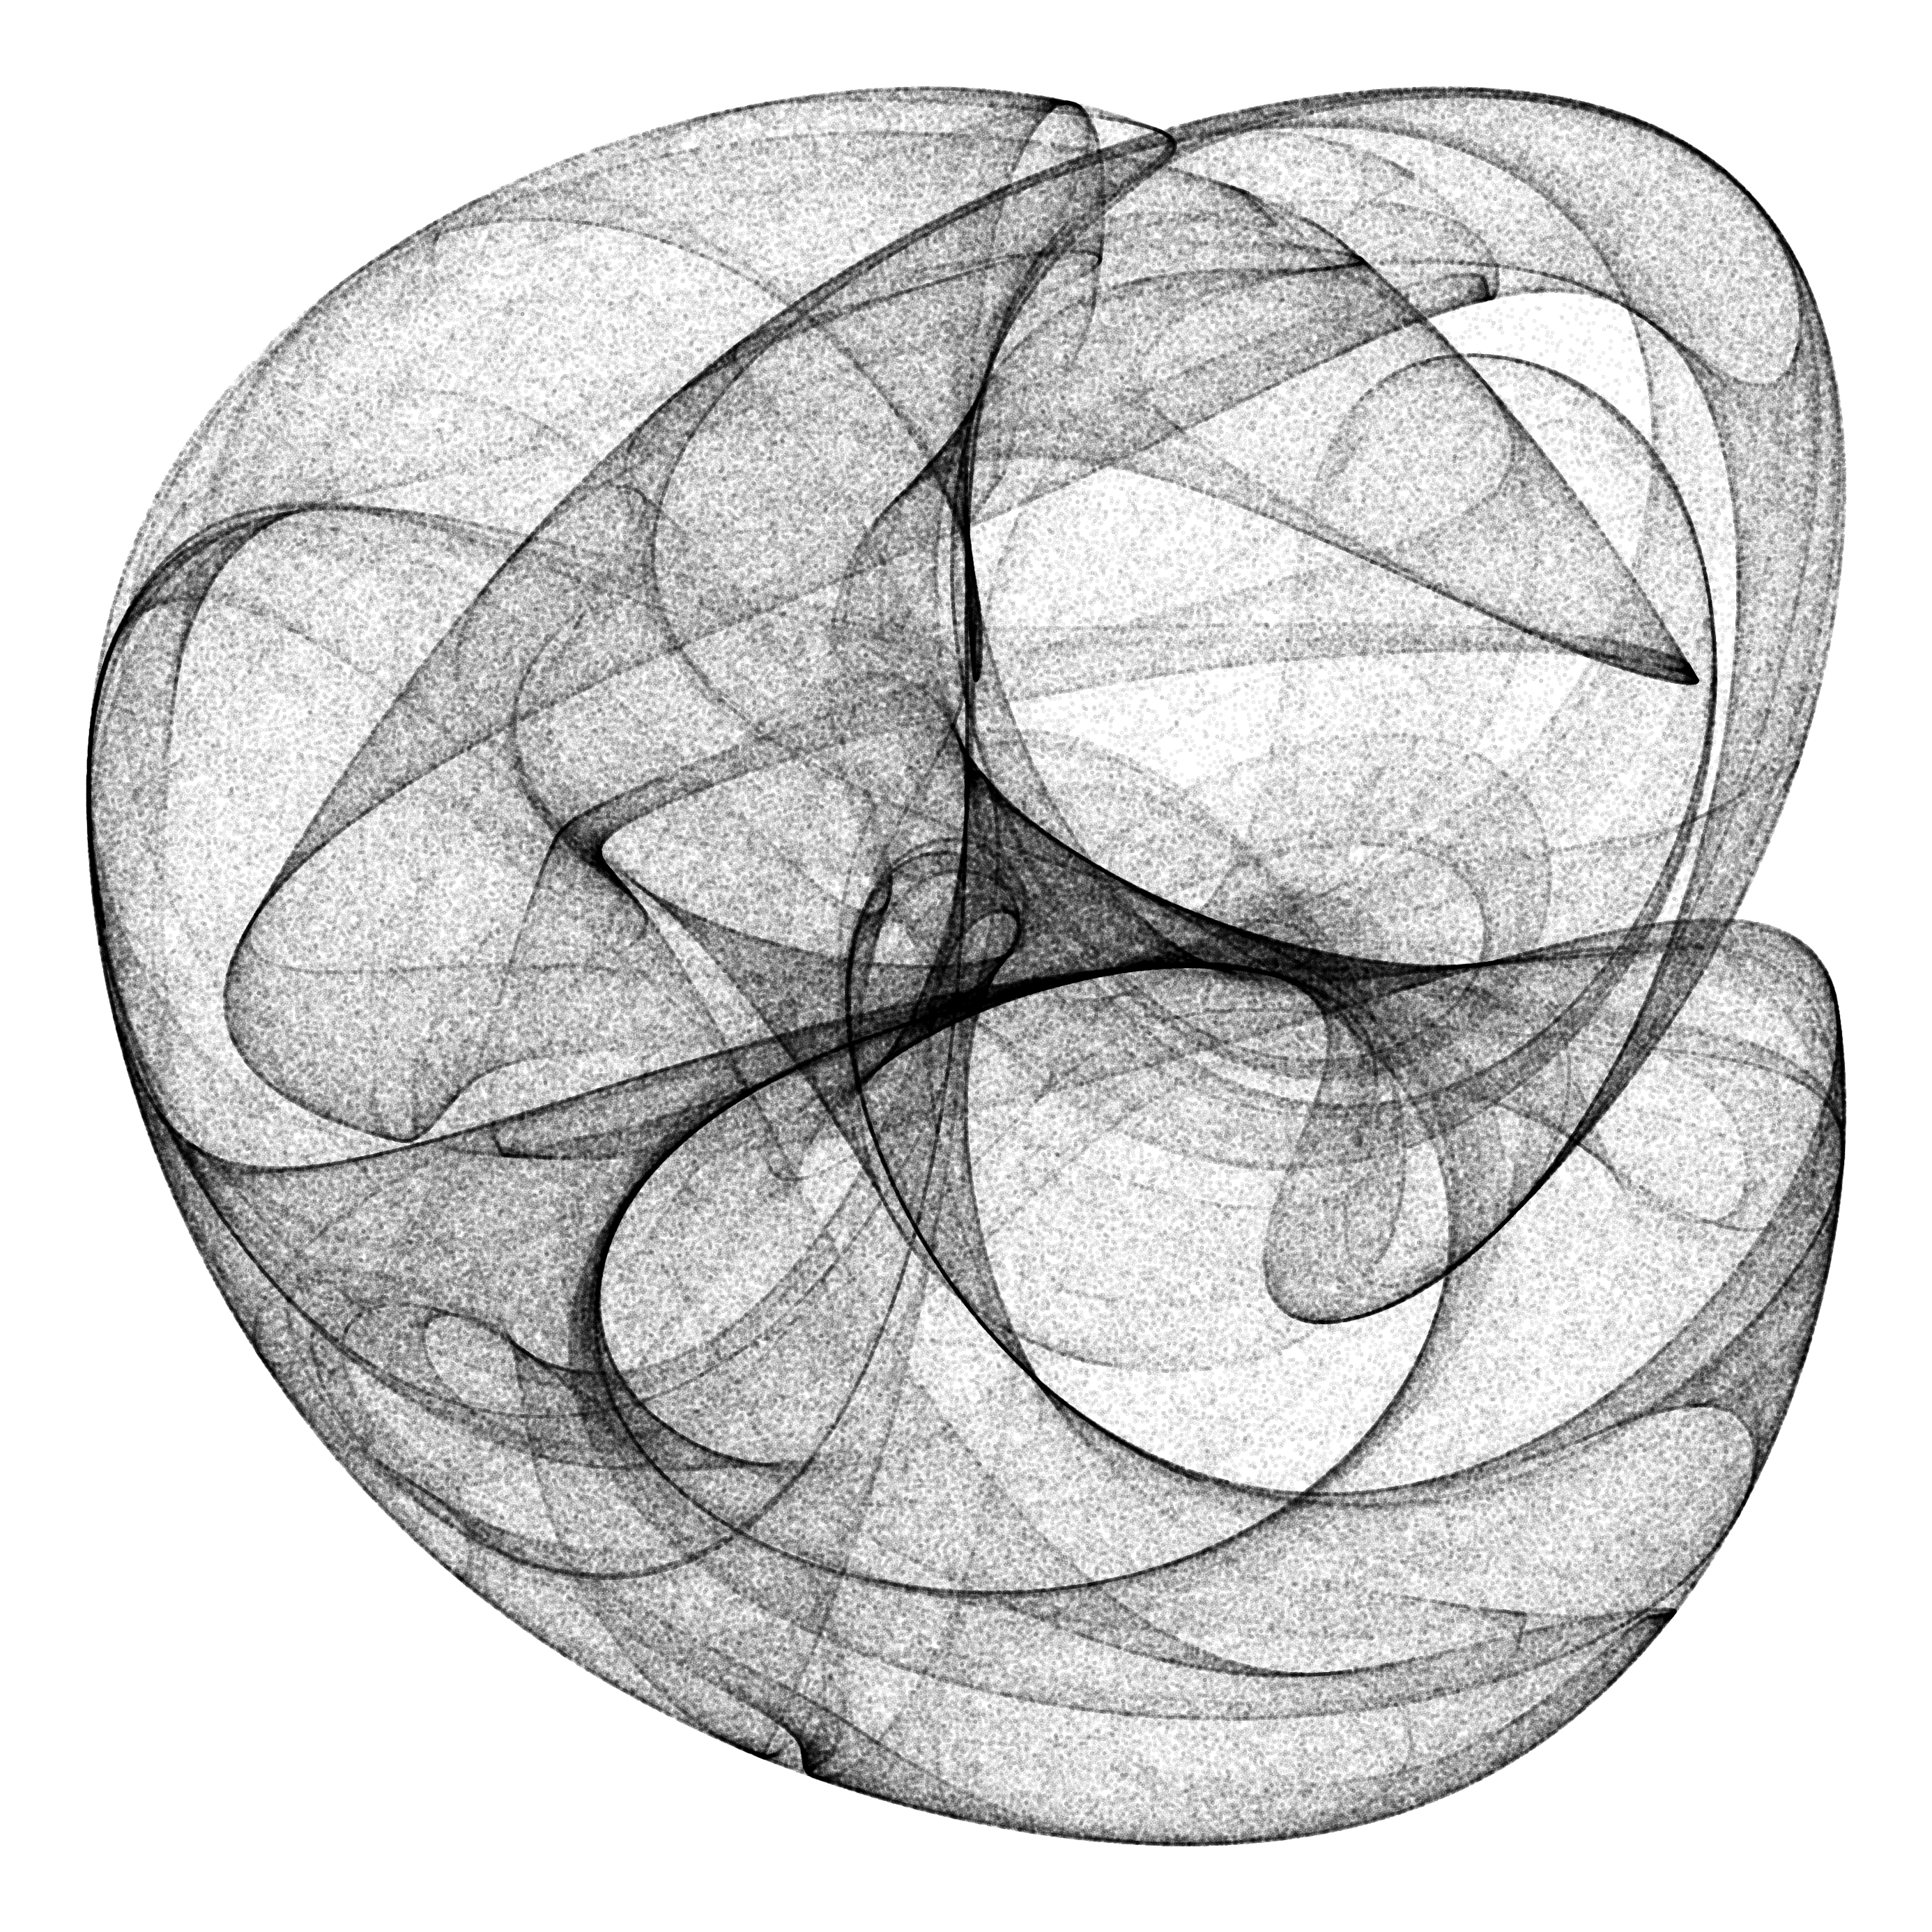
\includegraphics[width=.9\textwidth]{pics/dja.png}
    
    \vspace{2cm}
    
    % Uncomment the following line if you want to include a copyright
    % {\large \copyright\ 2024 \par}
    
    \vfill
\end{titlepage}

%-------------------- Subsequent Empty Pages --------------------
\newpage
\thispagestyle{empty}
\
\clearpage
\newpage

%-------------------- Second Page --------------------
\clearpage
\thispagestyle{empty}

\begin{center}
    \vspace*{4cm}
    {\Large \textbf{Theories of Generalized Change}} \\
    \vspace{1cm}
    {\Large \textit{Joseph J. Babčanec}} \\
    \vspace{2cm}
    {\Large First Edition} \\
    \vspace{1cm}
    {\Large \copyright\ 2025}
\end{center}

\clearpage

%-------------------- Dedication Page --------------------
\newpage
\thispagestyle{empty}
\vspace*{2cm}
\begin{center}
\itshape
To my wife Emily and my sons Andy and Jamie \\
To my former math teacher Heather Elfen
\end{center}
\vspace*{\fill}
\clearpage

%-------------------- Additional Empty Pages --------------------
\newpage
\thispagestyle{empty}
\
\clearpage

%-------------------- Copyright and Publishing Information --------------------
\newpage
\thispagestyle{empty}
\vspace*{2cm}

\noindent Theories of Generalized Change \\
First Edition

\vspace{1.2cm}

\noindent Copyright © 2025 by Joseph J. Babčanec

\noindent All rights reserved. No part of this publication may be reproduced, stored in a retrieval system, or transmitted, in any form or by any means—electronic, mechanical, photocopying, recording, or otherwise—without the prior written permission of the author, except in the case of brief quotations used in reviews or scholarly analysis.

\vspace{1.2cm}

\noindent Some illustrations in this book are original works by the author; others are sourced from public domain or free-to-use archives, and are credited where appropriate.

\vspace{1.2cm}

\noindent ISBN 978-1-23456-789-0

\vspace{1.2cm}

\noindent Cover design and interior layout by Joseph J. Babčanec

\vspace{1.2cm}

\noindent Printed in the United States of America

\vspace{1.2cm}

\noindent 10 9 8 7 6 5 4 3 2 1

\noindent First Printing, \the\year

\vfill

\noindent Set in \LaTeX\ using the Computer Modern typeface.
\newpage

%-------------------- Introduction Page Style --------------------
\fancypagestyle{intro}{
    \fancyhf{} % Clear all header and footer fields
    \fancyhead[R]{\textit{\MakeUppercase{Introduction}}} % Right-justified, italicized, and capitalized header
    \fancyfoot[C]{\thepage} % Page number in the center of the footer
}
\pagestyle{intro}

%-------------------- Table of Contents --------------------
\tableofcontents
% Start Roman numeral page numbering
\pagenumbering{roman}

%-------------------- Front Matter --------------------
\chapter*{Preface}

\noindent I wrote this textbook primarily to provide students of Multivariate Calculus (also known as Vector Calculus or Calculus III) with the option of having a concise reference to assist them or a springboard into deeper mathematical topics for the sake of interest. When I was a freshman engineering major in college, I reached this crossroads and, in a way, chose both paths—I added a mathematics major, thereby embracing both perspectives. These notes, compiled into textbook form and titled ``Theories of Generalized Change,'' are designed to bridge theory with application, emphasizing problem-solving techniques and the essential skills needed in applied fields. \\

\noindent This course, like most others, requires a solid foundation in Calculus I and Calculus II, including an understanding of limits, derivatives, integrals, and series. Reviewing the concepts from Calculus I will be particularly helpful before diving in, and knowledge from Calculus II will provide additional clarity and depth. While familiarity with introductory multivariable concepts is beneficial, we will introduce and review key topics as needed to ensure all students have the necessary tools to succeed. This course will feel like we are revisiting basic Differential Calculus, but with a new spirit—one of generalization. We will constantly explore how to further generalize and extend our understanding of Calculus to higher dimensions. \\

\noindent The course topics cover vectors, vector-valued functions, partial derivatives, multiple integrals, vector calculus theorems, introductory topics in Partial Differential Equations (PDEs), and a bit of Complex Variables, each presented with examples relevant to engineering, physics, and other applied sciences. PDEs and, less frequently, Complex Variables are seldom discussed in such a course. However, they are intrinsically tied together and embody the spirit of generalizing calculus; not to mention, they are quite useful in their own right. Through these applications, students will develop an appreciation for the power of calculus in modeling and solving practical problems, as well as gain a taste of higher mathematics. \\

\noindent Each chapter is divided into lectures, roughly structured to fit a 90- to 120-minute session. This format allows flexibility for instructors to adapt the material to the pace and needs of the class. The sections within each lecture focus on specific concepts, promoting a gradual mastery of each topic before progressing to more advanced material. This structure also provides a convenient framework for creating assignments and assessments. In my opinion, Chapters 1–5 are absolutely crucial for a Multivariate Calculus class, while Chapters 6 and 7 are additional topics to include if there is extra time. \\

\noindent One of the most challenging aspects for students of mathematics is handling notation and the over-assumptions made by some texts. Extra care is taken to ensure that notation is clearly defined and labeled—mathematics is like learning a new language. I also make sure to write out problems in full and use examples that cover a broad range of use cases, allowing students to more easily make connections to further topics. \\

\noindent My goal as an educator with this text is to empower students to apply multivariable calculus concepts beyond the classroom, equipping them with a robust mathematical foundation for their future studies and careers. I hope this course serves as a valuable resource for both students and instructors, providing the clarity, depth, and insight needed to master Multivariate Calculus...I also crack jokes often. Enjoy!
\\
\\
\\
\\
\\
Joseph J. Babčanec
\\
\\
Adjunct Professor of Mathematics, Benedict College
\\
Lead Data Scientist, Anika Systems Inc.
\\
\\
\href{mailto:joseph.babcanec@benedict.edu}{joseph.babcanec@benedict.edu}.
%%%%%%%introduction

\chapter*{Introduction}
\addcontentsline{toc}{chapter}{Introduction}

\section*{Purpose of This Book}
This book is structured to provide comprehensive coverage of Calculus III concepts, with applications relevant to fields such as engineering, physics, and applied sciences. The aim is to build on students' foundation in single-variable calculus, introducing the complexities of multivariable calculus and vector calculus. By focusing on practical and theoretical elements, the book equips students to understand multidimensional space, vector fields, integrals over curves and surfaces, and more advanced mathematical modeling techniques. \\ \\ This text is designed as a primary resource, integrating lecture material with detailed explanations, examples, and practice problems to foster a strong grasp of the subject.

\section*{How to Use This Book}
This book should be used as a guide and practice tool alongside lectures. Each section breaks down complex ideas, followed by examples and exercises. Students should:
\begin{itemize}
    \item \textbf{Preview Sections:} Familiarize yourself with topics before lectures for easier engagement.
    \item \textbf{Engage During Lectures:} Participate in discussions to solidify your understanding.
    \item \textbf{Work Through Examples:} Each example is chosen to illustrate key techniques.
    \item \textbf{Attempt Problems Independently:} Practice problems build problem-solving skills.
    \item \textbf{Use as Reference:} Refer back to specific sections when tackling homework or exams.
\end{itemize}

\section*{Overview of Chapters}
This book is organized into seven chapters, progressively covering essential topics in multivariable calculus and applications:

\begin{enumerate}
    \item \textbf{Vectors and the Geometry of Space:} Covers 3D coordinate systems, vector operations, lines, planes, and quadric surfaces, including applications in engineering.
    \item \textbf{Vector-Valued Functions and Motion in Space:} Explores vector functions, derivatives, motion along curves, curvature, arc length, and engineering applications.
    \item \textbf{Partial Derivatives:} Examines functions of several variables, limits, partial derivatives, chain rule, tangent planes, and optimization, crucial for multidimensional analysis.
    \item \textbf{Multiple Integrals:} Discusses double and triple integrals in various coordinates, with applications in area, volume, mass, and center of mass.
    \item \textbf{Vector Calculus:} Focuses on vector fields, line and surface integrals, and major theorems like Green’s, Stokes’, and the Divergence Theorem.
    \item \textbf{Differential Equations:} Introduces ODEs and PDEs with applications.
    \item \textbf{Complex Variables:} Covers basic complex analysis, including complex functions, integration, and applications in physics.

\end{enumerate}

\section*{Prerequisites}
This course requires a solid foundation in Calculus I and II. Students should be comfortable with:

\begin{itemize}
    \item \textbf{Differentiation and Integration:} Mastery of techniques for single-variable calculus.
    \item \textbf{Series and Sequences:} Familiarity with Taylor and power series.
    \item \textbf{Basic Linear Algebra:} Matrix operations and systems of linear equations are very helpful.
    \item \textbf{Mathematical Reasoning:} Ability to follow and construct rigorous proofs will ensure you get the very most out of this book.
\end{itemize}

\section*{Acknowledgments}
Special thanks to my colleagues and the mathematics department for their support and input. I also must of course mention my family who puts up with me when I write such textbooks (this is my third), and go bat-shit crazy for a few months.

\section*{Basic Terminology} \index{Basic Terminology}

Below is an extensive list of terms essential to Calculus III and related subject matter to be covered in this text.

\begin{description}

  \item[\textbf{3D Coordinate System}] A system for describing positions in three-dimensional space using three coordinates (e.g., $(x,y,z)$) relative to mutually perpendicular axes.

  \item[\textbf{Cartesian Coordinates}] A coordinate system in which points are described by their distances along perpendicular axes, typically labeled $x$, $y$, and $z$.

  \item[\textbf{Cylindrical Coordinates}] A three-dimensional coordinate system using $(r, \theta, z)$, where $r$ is the radius in the $xy$-plane, $\theta$ is the angle around the $z$-axis, and $z$ is the vertical coordinate.

  \item[\textbf{Spherical Coordinates}] A three-dimensional coordinate system using $(\rho, \theta, \phi)$, where $\rho$ is the distance from the origin, $\theta$ is the angle in the $xy$-plane, and $\phi$ is the angle from the positive $z$-axis.

  \item[\textbf{Vectors}] Quantities with both magnitude and direction, often represented as $\langle x, y, z \rangle$ in three dimensions.

  \item[\textbf{Magnitude (Norm) of a Vector}] The length of a vector, computed as $\sqrt{x^2 + y^2 + z^2}$ in 3D.

  \item[\textbf{Unit Vector}] A vector of length 1 in a particular direction.

  \item[\textbf{Dot Product}] An operation that takes two vectors and produces a scalar, measuring the extent to which they point in the same or opposite directions.

  \item[\textbf{Cross Product}] An operation that takes two vectors in 3D and produces a vector perpendicular to both, with magnitude related to the area of the parallelogram formed by the two vectors.

  \item[\textbf{Vector-Valued Functions}] Functions whose outputs are vectors, commonly written as $\mathbf{r}(t) = \langle x(t), y(t), z(t) \rangle$.

  \item[\textbf{Parametric Equations of Curves}] Expressions for $x$, $y$, and $z$ in terms of a parameter $t$, used to describe curves in three dimensions.

  \item[\textbf{Tangent Vector}] The derivative of a vector-valued function, indicating the instantaneous direction of the curve.

  \item[\textbf{Arc Length}] The length of a curve over an interval, computed by integrating the magnitude of the derivative of the vector-valued function.

  \item[\textbf{Curvature}] A measure of how sharply a curve bends at a given point.

  \item[\textbf{T, N, B (Frenet-Serret Frame)}] The unit tangent ($\mathbf{T}$), the principal normal ($\mathbf{N}$), and the binormal ($\mathbf{B}$) vectors associated with a curve in space.

  \item[\textbf{Level Surfaces}] Sets of points in 3D where a function of three variables is constant.

  \item[\textbf{Partial Derivatives}] Derivatives of a function of several variables with respect to one variable, treating the others as constants.

  \item[\textbf{Gradient}] A vector of all partial derivatives of a function, pointing in the direction of greatest increase.

  \item[\textbf{Directional Derivative}] The rate of change of a function in the direction of a specified vector.

  \item[\textbf{Chain Rule (Multivariable)}] A rule for computing the derivative of a composite function where the variables themselves depend on other parameters.

  \item[\textbf{Jacobian}] A determinant representing how a function of several variables transforms infinitesimal elements during a change of variables.

  \item[\textbf{Local Extrema (Maxima/Minima)}] Points where a function takes on locally highest or lowest values, found using partial derivatives and tests involving second derivatives.

  \item[\textbf{Saddle Point}] A point where a function is neither a local maximum nor a local minimum, but partial derivatives are zero.

  \item[\textbf{Multiple Integrals}] Integrals taken over regions in higher dimensions (e.g., double integrals over areas or triple integrals over volumes).

  \item[\textbf{Double Integral}] An integral over a two-dimensional region, typically written as $\iint_{D} f(x,y)\, dA$.

  \item[\textbf{Triple Integral}] An integral over a three-dimensional region, typically written as $\iiint_{E} f(x,y,z)\, dV$.

  \item[\textbf{Iterated Integrals}] The process of evaluating a multiple integral by integrating one variable at a time.

  \item[\textbf{Line Integrals}] Integrals that sum a function along a curve, with either scalar or vector integrands.

  \item[\textbf{Surface Integrals}] Integrals that sum a function over a surface in 3D, used for scalar fields or vector fields.

  \item[\textbf{Vector Fields}] Functions that assign a vector to each point in space, often denoted $\mathbf{F}(x,y,z)$.

  \item[\textbf{Divergence}] A scalar measure of how much a vector field spreads out or converges at a given point.

  \item[\textbf{Curl}] A vector measure of the rotation or swirling strength of a vector field at a point.

  \item[\textbf{Laplacian}] The sum of second partial derivatives of a function (in 3D, $\nabla^2 f = \frac{\partial^2 f}{\partial x^2} + \frac{\partial^2 f}{\partial y^2} + \frac{\partial^2 f}{\partial z^2}$).

  \item[\textbf{Green's Theorem}] Relates a line integral around a simple closed curve in the plane to a double integral over the region it encloses.

  \item[\textbf{Stokes' Theorem}] Relates a surface integral of the curl of a vector field to a line integral of the field around the boundary of the surface.

  \item[\textbf{Divergence Theorem (Gauss's Theorem)}] Relates the flux of a vector field through a closed surface to the volume integral of the divergence of the field over the region it encloses.

  \item[\textbf{Ordinary Differential Equations (ODEs)}] Equations involving derivatives of functions of one variable.

  \item[\textbf{Order of an ODE}] The highest derivative present in the equation (e.g., first-order, second-order).

  \item[\textbf{Linear ODE}] An ODE where the function and its derivatives appear to the first power and there are no products of the function and/or its derivatives.

  \item[\textbf{Nonlinear ODE}] An ODE that does not meet the criteria for linearity; may include products of the function and its derivatives or other nonlinear terms.

  \item[\textbf{Initial Value Problem (IVP)}] An ODE with specified initial conditions at a particular point.

  \item[\textbf{Partial Differential Equations (PDEs)}] Equations involving partial derivatives of functions of multiple variables (e.g., the heat equation or wave equation).

  \item[\textbf{Boundary Conditions}] Constraints specifying the values (or behavior) of a function along boundaries of a domain for PDEs.

  \item[\textbf{Complex Numbers}] Numbers of the form $z = x + iy$, where $i$ is the imaginary unit and $x,y$ are real.

  \item[\textbf{Complex Plane}] A two-dimensional plane representing the real part on the horizontal axis and the imaginary part on the vertical axis.

  \item[\textbf{Polar Form of a Complex Number}] Writing a complex number as $re^{i\theta}$, where $r$ is the magnitude and $\theta$ is the argument (angle).

  \item[\textbf{Complex Function}] A function with complex input and output, often written $f(z)$.

  \item[\textbf{Holomorphic (Analytic) Function}] A complex function that is differentiable everywhere in its domain, satisfying the Cauchy-Riemann equations.

  \item[\textbf{Contour}] A path or curve in the complex plane along which a complex integral can be computed.

  \item[\textbf{Residue}] A coefficient representing the behavior of a complex function near its singularity, used for evaluating contour integrals via the residue theorem.

  \item[\textbf{Contour Integral}] An integral of a complex function along a specified path in the complex plane.

  \item[\textbf{Euler's Formula}] A fundamental relationship $e^{i\theta} = \cos(\theta) + i\sin(\theta)$, connecting complex exponentials with trigonometric functions.

\end{description}


\section*{Mathematical Symbols and Notation} \index{Mathematical Symbols}

A comprehensive list of symbols used throughout Calculus III:

\begin{description}
    \item[$\vec{r}$, \textbf{r}] Position vector.
    \item[$|\vec{v}|$, $|\textbf{v}|$, $\| \textbf{v} \|$, $\|\textbf{v}\|_2$] Magnitude of vector $\vec{v}$.
    \item[$\Delta$] Finite Difference.
    \item[$\int$] Integral sign.
    \item[$\sum$] Summation.
    \item[$\prod$] Product.
    \item[$\nabla$] Del operator (used in gradient, divergence, curl).
    \item[$\partial$] Partial derivative symbol. Also used to indicate boundary, i.e., $\partial C$
    \item[$dA$, $dV$] Area and volume elements.
    \item[$\rho$, $\theta$, $\phi$] Spherical coordinates.
    \item[$\vec{F}$, \textbf{F}] Vector field.
    \item[$\int_C$] Line integral.
    \item[$\iint_S$] Surface integral.
    \item[$\iiint_V$] Triple integral.
    \item[$\oint_C$] Closed Contour Line integral.
    \item[$\oiint_S$] Closed Contour Surface integral.
    \item[$O$] Big $O$ notation.
    \item[$\approx$] Approximately equal.
    \item[$\equiv$] Identically equal.
    \item[$\perp$] Perpendicular.
    \item[$\parallel$] Parallel.
    \item[$\Rightarrow$] Implies.
\end{description}


\vspace{1em}

\noindent This book aims to provide a comprehensive understanding of these and other core concepts, supporting students in developing the mathematical maturity required for advanced studies and professional applications.

%-------------------- Main Content --------------------
% Reset page numbering to Arabic for the main content
\cleardoublepage
\pagenumbering{arabic}

% Define the custom page style for chapters
\fancypagestyle{mystyle}{
    \fancyhf{} % Clear all header and footer fields
    
    % Odd page: show chapter title only, right-aligned and italicized
    \fancyhead[RO]{\textit{\leftmark}} 
    
    % Even page: show chapter title and lecture title if available, left-aligned and italicized
    \fancyhead[LE]{%
        \textit{\leftmark} % Chapter title
        \ifnum\value{lecture}>0 : Lecture \thechapter.\thelecture \fi % Lecture title if exists
    }
    
    % Center the page number in the footer on all pages
    \fancyfoot[C]{\thepage}
}

% Apply the custom page style globally
\pagestyle{mystyle}

% Include chapters
%%%%%%%%%%%%%%%%%%%%%%%%%%%
\chapter{Single-Variable Calculus, Vectors, and the Geometry of Space}

\section*{Introduction}

In this chapter, we begin our journey into multivariable calculus by revisiting core concepts from Calculus I and Calculus II. These reviews will serve as stepping stones as we enter into the world of ``high-dimensional thinking." Our goal is to build a solid foundation for understanding functions that involve several variables, expanding beyond the single-variable functions studied previously. Functions of multiple variables naturally arise in physics and engineering. This chapter will introduce functions like these that depend on multiple variables, setting the stage for exploring complex systems where outcomes are influenced by more than one parameter. \\ \\To engage with these new concepts, we will introduce vectors, essential tools for representing quantities with both magnitude and direction. Vectors are critical for understanding spatial relationships and navigating the geometry of three-dimensional space. We will cover the fundamental operations on vectors, including addition, scalar multiplication, dot product, and cross product, each with significant applications in describing physical forces, directions, and motions. Furthermore, this chapter will introduce the geometry of space, specifically three-dimensional coordinate systems. By exploring Cartesian, cylindrical, and spherical coordinates, we will establish methods to describe points, lines, planes, and surfaces in space. These systems provide multiple ways of visualizing and solving problems, especially in fields like engineering and physics, where spatial reasoning and high-dimensional analysis are vital. \\ \\ In summary, this chapter lays the groundwork for high-dimensional thinking, equipping students with the skills to analyze functions of several variables and understand the fundamental geometry of space. With a thorough review of Calculus I and II concepts, we’ll be ready to explore multivariable calculus, ultimately deepening our ability to model and interpret complex systems.
\newpage


\lecture{Review of Differential and Integral Calculus}



\subsection*{Review of Single-Variable Calculus}\index{Calculus}

\noindent Before we embark on multivariable calculus, it’s essential to have a strong command of foundational topics in single-variable calculus, along with proficiency in algebra. Mastery of differentiation, integration, and limits forms the backbone of the more advanced concepts we’ll explore in this course. Additionally, skill in handling complex algebraic expressions will be invaluable, as calculus problems frequently require careful algebraic manipulation. These topics should already be second nature:

\begin{enumerate}
    \item \textbf{Limits and Continuity:}
    
    \noindent A precise understanding of limits is fundamental. You should be comfortable calculating limits both algebraically and conceptually, as they underpin differentiation, integration, and continuity. Key ideas include the \(\varepsilon\)-\(\delta\) definition of a limit, one-sided limits, and limits approaching infinity.
    
    \item \textbf{Differentiation:}
    
    \noindent Differentiation techniques such as the power rule, product rule, quotient rule, and chain rule must be second nature. In multivariate calculus, you will extend these rules to partial derivatives and gradients. Familiarity with applications of derivatives—such as optimization, related rates, and curve sketching—is also critical, as these concepts generalize to higher dimensions.

    \item \textbf{Integration:}
    
    \noindent Integration techniques such as substitution, integration by parts, and partial fraction decomposition will reappear in multivariable settings. Definite and indefinite integrals, as well as their geometric interpretations (e.g., areas under curves), are fundamental. In multivariate calculus, we’ll extend these concepts to double and triple integrals over various regions.

    \item \textbf{Fundamental Theorem of Calculus:}
    
    \noindent A firm grasp of the Fundamental Theorem of Calculus is crucial. This theorem connects differentiation and integration, and its higher-dimensional analogs—like Green’s Theorem, Stokes’ Theorem, and the Divergence Theorem—are central topics in multivariate calculus.

    \item \textbf{Algebraic Skills:}
    
    \noindent Proficiency in manipulating algebraic expressions is indispensable. Be comfortable simplifying complex fractions, solving linear and quadratic equations, and working with exponential and logarithmic functions. Multivariable calculus often involves tedious algebraic steps, and fluency here will prevent errors.
\end{enumerate}

\noindent As we review these topics, consider how they might extend into three dimensions and beyond. For example, differentiation in higher dimensions involves calculating partial derivatives, gradients, and directional derivatives. Similarly, integration evolves to include volume and surface calculations. These extensions will require you to adapt and expand the skills you’ve already mastered in single-variable calculus. \textbf{Think of this review not as a simple refresher, but as a foundation to support the complexities of three-dimensional calculus.} \\ \\ Before we review, lets knock out some elementary examples that should be second nature to you. If they are not easy to you, then it is \textbf{critical} that you ensure you are at the level to where they are before you proceed past this lecture.


\exampleline
\begin{example}
Evaluate the derivative of \( f(x) = x^2 e^x \).

\begin{solution}
We use the product rule, which states:
\[
\frac{d}{dx} f(x) = u(x)v'(x) + v(x)u'(x).
\]
Here, \( u(x) = x^2 \) and \( v(x) = e^x \). Compute:
\[
\frac{d}{dx}(x^2 e^x) = x^2 \cdot \frac{d}{dx}(e^x) + e^x \cdot \frac{d}{dx}(x^2).
\]
\[
= x^2 e^x + 2x e^x = e^x(x^2 + 2x).
\]
Thus, the derivative is \( f'(x) = e^x(x^2 + 2x) \).
\end{solution}
\end{example}
\exampleline
\begin{example}
Find the general solution to \( \int \frac{1}{1 - x} \, dx \).

\begin{solution}
We use substitution to evaluate the integral. Let \( u = 1 - x \), so \( du = -dx \). Rewrite the integral:
\[
\int \frac{1}{1 - x} \, dx = \int \frac{-1}{u} \, du.
\]
The integral of \( \frac{1}{u} \) is \( \ln|u| \). Substituting back \( u = 1 - x \), we obtain:
\[
\int \frac{1}{1 - x} \, dx = -\ln|1 - x| + C,
\]
where \( C \) is the constant of integration.
\end{solution}
\end{example}
\exampleline


\begin{example}
Solve the system of equations:
\[
\begin{aligned}
2x + y &= 5, \\
x - y &= 1.
\end{aligned}
\]

\begin{solution}
Add the equations to eliminate \( y \):
\[
2x + y + x - y = 5 + 1 \implies 3x = 6 \implies x = 2.
\]
Substitute \( x = 2 \) into \( 2x + y = 5 \):
\[
2(2) + y = 5 \implies 4 + y = 5 \implies y = 1.
\]
Thus, the solution is \( (x, y) = (2, 1) \).
\end{solution}
\end{example}
\exampleline




\subsubsection*{Single-Variable Limits} \index{Limits}

\noindent Limits are fundamental in calculus, allowing us to understand the behavior of functions as they approach specific values. They provide a rigorous framework for defining instantaneous rates of change, which are crucial for differentiation and integration. Limits help us analyze functions near points of interest, including points where the function may not be defined, making them indispensable in fields like physics and engineering. You may not have encountered the formal epsilon-delta definition, but it forms the mathematical foundation for how limits are defined precisely.
\index{Limit Rules}
\begin{itemize}

\item \textbf{Definition}: $\lim_{x \to a} f(x) = L$ means that as $x$ approaches $a$, $f(x)$ gets arbitrarily close to $L$.

\item \textbf{Properties}:
\begin{itemize}
\item \textbf{Sum Rule}: $$\lim_{x \to a} [f(x) + g(x)] = \lim_{x \to a} f(x) + \lim_{x \to a} g(x)$$
\item \textbf{Product Rule}: $$\lim_{x \to a} [f(x)g(x)] = \lim_{x \to a} f(x) \cdot \lim_{x \to a} g(x)$$
\item \textbf{Quotient Rule}: $$\lim_{x \to a} \frac{f(x)}{g(x)} = \frac{\lim_{x \to a} f(x)}{\lim_{x \to a} g(x)}, \text{ if } \lim_{x \to a} g(x) \neq 0$$
\end{itemize}

\item \textbf{Single-Sided Limits}: \index{Single-Sided Limits}
Sometimes we are interested in the behavior of $f(x)$ as $x$ approaches $a$ from only one side, either from the left or the right.

\begin{itemize}
\item \textbf{Left-Hand Limit}: $\lim_{x \to a^-} f(x) = L$ means $f(x)$ approaches $L$ as $x$ approaches $a$ from values less than $a$.
\item \textbf{Right-Hand Limit}: $\lim_{x \to a^+} f(x) = L$ means $f(x)$ approaches $L$ as $x$ approaches $a$ from values greater than $a$.
\item For the (two-sided) limit $\lim_{x \to a} f(x) = L$ to exist, both the left-hand limit and right-hand limit must exist and be equal.
\end{itemize}

\item \textbf{Limits at Infinity and Infinite Limits}: \index{Infinite Limits}
In addition to limits at finite values, we often need to consider what happens to $f(x)$ as $x$ grows arbitrarily large or small, or as $f(x)$ approaches infinity.

\begin{itemize}
\item \textbf{Limit at Infinity}: $\lim_{x \to \infty} f(x) = L$ means that as $x$ becomes very large, $f(x)$ approaches $L$.
\item \textbf{Infinite Limit}: $\lim_{x \to a} f(x) = \infty$ means that as $x$ approaches $a$, $f(x)$ grows without bound.
\end{itemize}

\item \textbf{Formal Definition of a Limit (Epsilon-Delta Definition)}: \index{Epsilon-Delta Definition of Limits}
To define limits rigorously, we use the epsilon-delta definition, which formalizes the concept as follows: We say that $\lim_{x \to a} f(x) = L$ if for every $\epsilon > 0$, there exists a $\delta > 0$ such that:
\[0 < |x - a| < \delta \implies |f(x) - L| < \epsilon\]

This definition means we can make $f(x)$ as close to $L$ as desired (within $\epsilon$) by taking $x$ sufficiently close to $a$ (within $\delta$), without $x$ being exactly $a$.

\begin{figure}[H]
    \centering
\begin{tikzpicture}
  % Define the function
  \draw[domain=-1:5,smooth,variable=\x,blue] plot ({\x},{-1/exp(\x) + 5});
  
  % Horizontal line at L
  \draw[dashed,red] (-1,5) -- (5,5);
  \node[right,red] at (5,5) {$L$};
  
  % Horizontal epsilon bands
  \draw[dashed] (-1,5.5) -- (5,5.5);
  \node[right] at (5,5.5) {$L+\epsilon$};
  \draw[dashed] (-1,4.5) -- (5,4.5);
  \node[right] at (5,4.5) {$L-\epsilon$};
  
  % Vertical line at a
  \draw[dashed,red] (2,-0.5) -- (2,5.5);
  \node[below,red] at (2,-0.5) {$a$};
  
  % Vertical delta bands
  \draw[dashed] (1,-0.5) -- (1,5.5);
  \node[below] at (1,-0.5) {$a-\delta$};
  \draw[dashed] (3,-0.5) -- (3,5.5);
  \node[below] at (3,-0.5) {$a+\delta$};
  
  % Axis
  \draw[->] (-1,0) -- (6,0) node[right] {$x$};
  \draw[->] (0,-0.5) -- (0,6) node[above] {$f(x)$};
  
  % Point (a, L)
  \filldraw[red] (2,5) circle (2pt);
  \node[below right] at (2,5) {$(a, L)$};
  
\end{tikzpicture}
    \caption{\textit{A limit being approached notated with $\epsilon-\delta$ notation.}}
\end{figure}

\item \textbf{L'Hôpital's Rule}: \index{L'Hôpital's Rule}
When calculating limits, we sometimes encounter indeterminate forms, such as $\frac{0}{0}$ or $\frac{\infty}{\infty}$. L'Hôpital's Rule is a powerful tool for handling these cases. 

    If $\lim_{x \to a} f(x) = \lim_{x \to a} g(x) = 0$ or $\pm \infty$, and both \( f \) and \( g \) are differentiable near \( a \) (except possibly at \( a \)), then:
    \[
    \lim_{x \to a} \frac{f(x)}{g(x)} = \lim_{x \to a} \frac{f'(x)}{g'(x)}
    \]
    Provided the limit on the right exists or is infinite. L'Hôpital's Rule can also be applied iteratively. If an indeterminate form persists after applying the rule once, we may apply the rule again to the resulting expression until the limit can be evaluated.

\item \textbf{Interpreting the Epsilon-Delta Definition}:
  \begin{itemize}
  \item $\epsilon$ represents the desired closeness of $f(x)$ to $L$.
  \item $\delta$ is how close $x$ needs to be to $a$ to ensure $f(x)$ is within $\epsilon$ of $L$.
  \item The limit $\lim_{x \to a} f(x) = L$ exists if, for any chosen $\epsilon$, there is always a corresponding $\delta$ that keeps $f(x)$ within the desired range.
  \end{itemize}
\end{itemize}

\exampleline
\begin{example}
Use L'Hôpital's Rule to evaluate \( \lim_{x \to 0} \frac{e^x - 1 - x - \frac{x^2}{2}}{x^3} \).

\begin{solution}
Since both the numerator and denominator approach 0 as \( x \to 0 \), this is an indeterminate form of \( \frac{0}{0} \). We can apply L'Hôpital's Rule by differentiating the numerator and the denominator.

\begin{enumerate}
    \item Differentiate the numerator and denominator:
    \[
    \lim_{x \to 0} \frac{e^x - 1 - x - \frac{x^2}{2}}{x^3} = \lim_{x \to 0} \frac{\frac{d}{dx}(e^x - 1 - x - \frac{x^2}{2})}{\frac{d}{dx}(x^3)} = \lim_{x \to 0} \frac{e^x - 1 - x}{3x^2}
    \]

    \item This still gives an indeterminate form \( \frac{0}{0} \), so we apply L'Hôpital's Rule again:
    \[
    \lim_{x \to 0} \frac{e^x - 1 - x}{3x^2} = \lim_{x \to 0} \frac{\frac{d}{dx}(e^x - 1 - x)}{\frac{d}{dx}(3x^2)} = \lim_{x \to 0} \frac{e^x - 1}{6x}
    \]

    \item Apply L'Hôpital's Rule one more time:
    \[
    \lim_{x \to 0} \frac{e^x - 1}{6x} = \lim_{x \to 0} \frac{\frac{d}{dx}(e^x - 1)}{\frac{d}{dx}(6x)} = \lim_{x \to 0} \frac{e^x}{6}
    \]

    \item Evaluate the limit:
    \[
    \frac{e^0}{6} = \frac{1}{6}
    \]
\end{enumerate}
\end{solution}
\end{example}
\exampleline
\begin{example}
Prove using the epsilon-delta definition that \( \lim_{x \to 3} (2x + 5) = 11 \).

\begin{solution}
To prove this limit using the epsilon-delta definition, we need to show that for every \( \epsilon > 0 \), there exists a \( \delta > 0 \) such that whenever \( 0 < |x - 3| < \delta \), we have \( |(2x + 5) - 11| < \epsilon \).

\begin{enumerate}
    \item Start by simplifying \( |(2x + 5) - 11| \):
    \begin{align*}
    |(2x + 5) - 11| &= |2x - 6| \\
    &= |2(x - 3)| \\
    &= 2 |x - 3|
    \end{align*}

    \item We want \( |2(x - 3)| < \epsilon \). This can be achieved by ensuring that:
    \[
    2 |x - 3| < \epsilon
    \]
    or equivalently,
    \[
    |x - 3| < \frac{\epsilon}{2}
    \]

    \item Therefore, we can choose \( \delta = \frac{\epsilon}{2} \). Now, if \( 0 < |x - 3| < \delta \), then:
    \[
    |x - 3| < \frac{\epsilon}{2}
    \]
    which implies that:
    \[
    2 |x - 3| < 2 \cdot \frac{\epsilon}{2} = \epsilon
    \]

    \item Thus, \( |(2x + 5) - 11| < \epsilon \), as required.
\end{enumerate}
\end{solution}
\end{example}
\exampleline

\subsubsection*{Single-Variable Derivatives}\index{Derivatives}

Calculus is fundamentally the theory of change, providing tools to understand and quantify how quantities evolve in relation to one another. In single-variable calculus, derivatives play a central role in this theory, allowing us to determine the rate at which a function changes at any given point. The derivative of a function represents the slope of the tangent line to the function’s graph, encapsulating the concept of instantaneous change, or how the function behaves at an exact point in time or space. Derivatives have widespread applications across various fields, enabling us to calculate velocity and acceleration in physics, model growth rates in biology, and analyze marginal changes in economics, among others. \\ \\ As we progress in our study of calculus, we aim to extend this powerful framework by adding more variables, moving from single-variable functions to functions of several variables. This generalization will enable us to explore more complex systems where multiple factors interact, paving the way for multivariable calculus. Hence, this book is titled \textit{Theories of Generalized Change}, as we will develop the tools to analyze and model change not just in one direction or along one axis, but across multiple dimensions and variables, broadening the scope and applicability of calculus. \\ \\ To start with, derivatives are grounded in the concept of the \textbf{Instantaneous Rate of Change} (IROC), which refines the \textbf{Average Rate of Change} (AROC) by focusing on how a function behaves “at a single point.” While AROC provides the rate of change over a finite interval, IROC captures the behavior as this interval shrinks to zero, giving us a precise measure of change at an infinitesimal level. This approach of taking limits is foundational in calculus and will serve as the basis for more advanced studies in differentiation and integration.


\begin{itemize}
\item \textbf{Average Rate of Change (AROC)}:
The AROC of a function \( f(x) \) over an interval \( [a, b] \) is given by:
\[
\text{AROC} = \frac{f(b) - f(a)}{b - a}
\]
This is the slope of the secant line between the points \( (a, f(a)) \) and \( (b, f(b)) \) on the graph of \( f \). The AROC gives an overall measure of change across the interval, providing insights but not specifics about any single point within that interval.


\begin{figure}[H]
\begin{center}
\begin{tikzpicture}[scale=1.75,cap=round]
\tikzset{axes/.style={}}
%\draw[style=help lines,step=1cm, dotted] (-5.25,-5.25) grid (5.25,5.25);
% The graphic
\begin{scope}[style=axes]
\draw[->] (-.5,0) -- (4.5,0) node[below] {$x$};
\draw[->] (0,-.5)-- (0,3) node[left] {$y$};
\foreach \x/\xtext in {1.5/a, 3/b}
 \draw[xshift=\x cm] (0pt,2pt) -- (0pt,-2pt) 
node[below,fill=white,font=\normalsize]
  {$\xtext$};    
\foreach \y/\ytext in {1/f(a), 2.125/f(b)}
  \draw[yshift=\y cm] (2pt,0pt) -- (-2pt,0pt) 
  node[left,fill=white,font=\normalsize]
  {$\ytext$};
  %%%
 \draw[domain=.5:3.25,smooth,variable=\x,red,<->,thick] plot ({\x},{.5*(\x-1.5)*(\x-1.5)+1});
  %%%
\filldraw[black] (1.5,1) circle (1pt) node[above] {\scriptsize $P$};
\filldraw[black] (3,2.125) circle (1pt) node[left] {\scriptsize $Q$};
\draw[thick,blue!70!black,shorten >=-.5cm,shorten <=-.5cm] (1.5,1)--(3,2.125) 
node[midway,left] {\scriptsize Secant Line};
 %%%
 \draw[blue!70!black,thick,dashed] (1.5,1)--(3,1)--(3,2.125);
 \draw[blue!70!black] (3,1.1)--(2.9,1.1)--(2.9,1);
 \draw[decoration={brace,mirror,raise=5pt},decorate,blue!70!black]
    (1.5,-.250) -- node[below=6pt] {$b-a$} (3,-.250);
 \draw[decoration={brace,mirror, raise=5pt},decorate,blue!70!black]
    (3,1) -- node[right=6pt] {$f(b)-f(a)$} (3,2.215);
 %%%
\filldraw[black] (1.5,1) circle (1pt) node[above] {\scriptsize $P$};
\filldraw[black] (3,2.125) circle (1pt) node[left] {\scriptsize $Q$};
\end{scope}
\end{tikzpicture}
\caption{\textit{A secant line threading two points along a curve \(f(x)\).}}
\end{center}
\end{figure}


\item \textbf{Instantaneous Rate of Change (IROC)}:
While AROC provides an average, we often seek to know how fast the function is changing at a specific point. The IROC at a point \( x = a \) is the derivative of the function, calculated as the limit of the AROC as the interval becomes infinitesimally small.

\item \textbf{Definition of the Derivative (Single Variable)}:
For a function \( f(x) \), the derivative at a point \( x = a \) is defined by the limit:
\[
f'(a) = \lim_{h \to 0} \frac{f(a + h) - f(a)}{h}
\]
This expression represents the slope of the tangent line to \( f \) at the point \( (a, f(a)) \), capturing the instantaneous rate of change of \( f(x) \) with respect to \( x \) at \( a \).


\begin{figure}[H]
\begin{center}
\begin{tikzpicture}[scale=1.75,cap=round]
\tikzset{axes/.style={}}
%\draw[style=help lines,step=1cm, dotted] (-5.25,-5.25) grid (5.25,5.25);
% The graphic
\begin{scope}[style=axes]
\draw[->] (-.5,0) -- (4.5,0) node[below] {$x$};
\draw[->] (0,-.5)-- (0,3) node[left] {$y$};
\foreach \x/\xtext in {1.5/a}
 \draw[xshift=\x cm] (0pt,2pt) -- (0pt,-2pt) 
node[below,fill=white,font=\normalsize]
  {$\xtext$};    
\foreach \y/\ytext in {1/f(a)}
  \draw[yshift=\y cm] (2pt,0pt) -- (-2pt,0pt) 
  node[left,fill=white,font=\normalsize]
  {$\ytext$};
  %%%
 \draw[domain=.5:3.25,smooth,variable=\x,red,<->,thick] plot ({\x},{.5*(\x-1.5)*(\x-1.5)+1});
  %%%
\filldraw[black] (1.5,1) circle (1pt) node[above] {\scriptsize $P$};
% Draw tangent line at P (horizontal line)
\draw[thick,blue] (0.5,1) -- (2.5,1) 
node[midway,below=6pt] {\scriptsize \textbf{Tangent Line}};
 %%%
\end{scope}
\end{tikzpicture}
\caption{\textit{A tangent line threadinga point along a curve \(f(x)\).}}
\end{center}
\end{figure}


\item \textbf{Basic Derivative Rules}\index{Derivative Rules}
The following rules simplify the process of finding derivatives for common functions.

\begin{itemize}
\item \textbf{Power Rule}: If \( f(x) = x^n \), then
\[
f'(x) = nx^{n-1}
\]
\item \textbf{Exponential Rule}: If \( f(x) = e^x \), then
\[
f'(x) = e^x
\]
\item \textbf{Logarithmic Rule}: If \( f(x) = \ln(x) \), then
\[
f'(x) = \frac{1}{x}
\]
\item \textbf{Sine Rule}: If \( f(x) = \sin(x) \), then
\[
f'(x) = \cos(x)
\]
\item \textbf{Cosine Rule}: If \( f(x) = \cos(x) \), then
\[
f'(x) = -\sin(x)
\]
\end{itemize}

\item \textbf{Product and Quotient Rules}\index{Product Rule}\index{Quotient Rule}
When dealing with the derivatives of products or quotients of functions, we use these rules:

\begin{itemize}
\item \textbf{Product Rule}: If \( f(x) = u(x)v(x) \), then
\[
f'(x) = u'(x)v(x) + u(x)v'(x)
\]
\item \textbf{Quotient Rule}: If \( f(x) = \frac{u(x)}{v(x)} \), then
\[
f'(x) = \frac{u'(x)v(x) - u(x)v'(x)}{[v(x)]^2}
\]
\end{itemize}

\item \textbf{Chain Rule}\index{Chain Rule}
For composite functions, we use the Chain Rule:

If \( f(x) = g(h(x)) \), then
\[
f'(x) = g'(h(x)) \cdot h'(x)
\]
The Chain Rule is essential when differentiating functions nested within other functions, allowing us to find the derivative of more complex expressions.

\end{itemize}

\exampleline
\begin{example}
Use the limit definition of the derivative to find the derivative of the function \( f(x) = x^2 \).

\begin{solution}
The derivative of \( f(x) = x^2 \) at a point \( x \) can be found using the limit definition of the derivative:
\[
f'(x) = \lim_{h \to 0} \frac{f(x+h) - f(x)}{h}
\]
\begin{enumerate}
    \item Substitute \( f(x) = x^2 \) into the formula:
    \[
    f'(x) = \lim_{h \to 0} \frac{(x+h)^2 - x^2}{h}
    \]
    \item Expand \( (x+h)^2 \):
    \[
    f'(x) = \lim_{h \to 0} \frac{x^2 + 2xh + h^2 - x^2}{h}
    \]
    \item Simplify by canceling \( x^2 \) terms:
    \[
    f'(x) = \lim_{h \to 0} \frac{2xh + h^2}{h}
    \]
    \item Factor out \( h \) from the numerator:
    \[
    f'(x) = \lim_{h \to 0} \frac{h(2x + h)}{h}
    \]
    \item Cancel \( h \) in the numerator and denominator:
    \[
    f'(x) = \lim_{h \to 0} (2x + h)
    \]
    \item Take the limit as \( h \to 0 \):
    \[
    f'(x) = 2x
    \]
\end{enumerate}
\end{solution}
\end{example}

% Place a single blue line after the example
\exampleline


\subsubsection*{Integrals} \index{Integrals}

Integrals form a foundational concept in calculus, representing the accumulation of quantities and the area under a curve. Integrals have applications across mathematics and science, such as calculating area, volume, work, and in modeling the behavior of physical systems. The process of integration is often considered the reverse operation of differentiation, and it provides insights into quantities that are accumulated or summed continuously over intervals. In this section, we will explore the integral as a limit of finite sums (Riemann Sum), develop the concept of definite and indefinite integrals, and introduce several integration techniques. 

\begin{itemize}
\item \textbf{Indefinite Integral}:  \index{Indefinite Integrals}
The indefinite integral of a function \( f(x) \), also known as the antiderivative, is defined as:
\[
\int f(x) \, dx = F(x) + C
\]
where \( F'(x) = f(x) \) and \( C \) is the constant of integration. This represents the family of all antiderivatives of \( f(x) \), capturing the essence of the function’s accumulated effect.

\item \textbf{Definite Integral}: \index{Definite Integrals}
The definite integral of \( f(x) \) over the interval \([a, b]\) is defined as:
\[
\int_a^b f(x) \, dx = F(b) - F(a)
\]
where \( F(x) \) is any antiderivative of \( f(x) \). The definite integral represents the net area between the curve \( f(x) \) and the \( x \)-axis from \( x = a \) to \( x = b \), taking into account areas above and below the axis.

\item \textbf{Riemann Sum and the Integral as a Limit of Finite Sums}: \index{Riemann Sum}
The concept of integration can be understood through the Riemann Sum, which approximates the area under a curve by summing the areas of rectangles. As the number of rectangles increases (and their width decreases), the sum approaches the exact area under the curve.

For a function \( f(x) \) over \([a, b]\), we divide the interval into \( n \) subintervals, each of width \( \Delta x = \frac{b - a}{n} \). The Riemann sum is:
\[
\sum_{i=1}^n f(x_i^*) \Delta x
\]
where \( x_i^* \) is a sample point within each subinterval. The definite integral is defined as the limit of this sum as \( n \to \infty \):
\[
\int_a^b f(x) \, dx = \lim_{n \to \infty} \sum_{i=1}^n f(x_i^*) \Delta x
\]

\begin{figure}[H]
\begin{center}
\begin{tikzpicture}[scale=1.2,declare function={f(\x)=((1/3)*(\x)^(3)-3*(\x)^(2)+8*\x-3;}]
\coordinate (start) at (.8,{f(.8)});
\coordinate (x0) at (1,{f(1)});
\coordinate (x1) at (2,{f(2)});
\coordinate (x2) at (3,{f(3)});
\coordinate (x3) at (4,{f(4)});
\coordinate (x4) at (5,{f(5)});
\coordinate (end) at (5.05,{f(5.05)});
\draw[fill=orange!40!white] (1,0) rectangle (2,{f(1)});
\draw[fill=orange!40!white] (2,0) rectangle (3,{f(2)});
\draw[fill=orange!40!white] (3,0) rectangle (4,{f(3)});
\draw[fill=orange!40!white] (4,0) rectangle (5,{f(4)});
\draw (5,0)--(5,{f(5)});
\draw [-latex] (-0.5,0) -- (6,0) node (xaxis) [below] {$x$};
\draw [-latex] (0,-0.5) -- (0,5) node [left] {$y$};
\foreach \x/\xtext in {1/a=x^*_{1} ,2/x^*_{2}, 3/x^*_{3} , 4/x^*_{4} , 5/b }
 \draw[xshift=\x cm] (0pt,3pt) -- (0pt,0pt) 
node[below=2pt,fill=white,font=\normalsize]
  {$\xtext$};
\draw[domain=.5:5.3,samples=200,variable=\x,red,<->,thick] plot ({\x},{f(\x)});                 
\foreach \n in {0,1,2,3}
\draw[red,fill=red] (x\n) circle (2pt) node[font=\normalsize] {$$};    
\draw[<->] (2,-1)--(3,-1) node[above,midway] {$\Delta x$};      
\end{tikzpicture}
\caption{\textit{A Riemann Sum approximation for an integral of a function.}}
\end{center}
\end{figure}

\index{Integral Approximations}
\item \textbf{Approximations Using Left, Right, and Center Points; Maxima, Minima, Supremum, and Infimum}: \index{Approximations in Riemann Sums}
Riemann sums allow for different choices of points within each subinterval to approximate the integral. These choices influence the accuracy and convergence of the sum, providing different approximations based on the choice of evaluation points within each subinterval.

\begin{itemize}
\item \textbf{Left Endpoint Approximation}: The function is evaluated at the left endpoint of each subinterval \( x_i \), producing a sum that may underestimate the area for increasing functions and overestimate for decreasing functions. The Riemann sum for \( n \) subintervals of width \( \Delta x = \frac{b - a}{n} \) is:
\[
\sum_{i=0}^{n-1} f(x_i) \, \Delta x
\]
where \( x_i = a + i \Delta x \) represents the left endpoint of each subinterval.

\item \textbf{Right Endpoint Approximation}: The function is evaluated at the right endpoint of each subinterval \( x_{i+1} \). This sum tends to overestimate for increasing functions and underestimate for decreasing functions:
\[
\sum_{i=1}^{n} f(x_{i+1}) \, \Delta x
\]
where \( x_i = a + i \Delta x \) represents the right endpoint of each subinterval.

\item \textbf{Midpoint (Center) Approximation}: The function is evaluated at the midpoint \( x_i^* = \frac{x_i + x_{i+1}}{2} \) of each subinterval. This approach often yields a more accurate approximation by balancing overestimates and underestimates:
\[
\sum_{i=0}^{n-1} f\left(x_i^*\right) \, \Delta x
\]
where \( x_i^* = a + \left(i + \frac{1}{2}\right) \Delta x \) is the midpoint.

\item \textbf{Maximal Approximation}: For each subinterval \( [x_i, x_{i+1}] \), choose the maximum function value, yielding an upper bound for the area:
\[
\sum_{i=0}^{n-1} \max_{x \in [x_i, x_{i+1}]} f(x) \, \Delta x
\]
This approximation gives an upper bound for the integral if \( f(x) \) is continuous over \([a, b]\).

\item \textbf{Minimal Approximation}: Similarly, choosing the minimum function value within each subinterval provides a lower bound:
\[
\sum_{i=0}^{n-1} \min_{x \in [x_i, x_{i+1}]} f(x) \, \Delta x
\]
This approximation serves as a lower bound if \( f(x) \) is continuous over \([a, b]\).

\item \textbf{Supremum and Infimum}: \index{Supremum and Infimum}
For theoretical purposes and cases with countably many discontinuous points, we can define Riemann sums using the supremum (least upper bound) and infimum (greatest lower bound) of \( f(x) \) on each subinterval, providing bounds as \( n \to \infty \). This approach is foundational in defining integrability:
\[
\sum_{i=0}^{n-1} \sup_{x \in [x_i, x_{i+1}]} f(x) \, \Delta x \quad \text{and} \quad \sum_{i=0}^{n-1} \inf_{x \in [x_i, x_{i+1}]} f(x) \, \Delta x
\]
These sums approximate the true integral more closely as \( n \to \infty \).
\end{itemize}

\item \textbf{Numerical Integration Techniques} \index{Numerical Integration}
When exact integration is challenging, numerical integration methods approximate the value of definite integrals by evaluating the function at specific points. Key methods include:
\begin{itemize}
\item \textbf{Trapezoidal Rule}: Approximates the area under the curve by dividing it into trapezoids rather than rectangles, averaging the left and right endpoint evaluations: \index{Trapezoidal Rule}
\[
\int_a^b f(x) \, dx \approx \frac{\Delta x}{2} \left[ f(x_0) + 2\sum_{i=1}^{n-1} f(x_i) + f(x_n) \right]
\]
where \( \Delta x = \frac{b - a}{n} \) and \( x_0, x_1, \dots, x_n \) are equally spaced points.

\item \textbf{Simpson's Rule}: \index{Simpson's Rule} Uses parabolic segments to approximate the curve. It is more accurate for functions that are reasonably smooth and is defined as:
\[
\int_a^b f(x) \, dx \approx \frac{\Delta x}{3} \left[ f(x_0) + 4\sum_{\text{odd } i} f(x_i) + 2\sum_{\text{even } i} f(x_i) + f(x_n) \right]
\]
\end{itemize}
Simpson’s Rule provides excellent accuracy for a modest number of intervals, especially for polynomials and smooth functions.


\exampleline
\begin{example}
Use Simpson's Rule with \( n = 4 \) subintervals to approximate the integral \( \int_0^{2} \frac{1}{1 + x^2} \, dx \). Compare the result with the exact value of the integral.

\begin{solution}
Since Simpson's Rule requires knowing the exact value to compare, we start by calculating the exact value of the integral:
\[
\int_0^{2} \frac{1}{1 + x^2} \, dx = \left[ \arctan x \right]_0^2 = \arctan 2 - \arctan 0 = \arctan 2.
\]

\begin{enumerate}
    \item Calculate the width of each subinterval:
    \[
    h = \frac{b - a}{n} = \frac{2 - 0}{4} = 0.5.
    \]

    \item Determine the \( x \)-values:
    \[
    x_0 = 0,\quad x_1 = 0.5,\quad x_2 = 1.0,\quad x_3 = 1.5,\quad x_4 = 2.0.
    \]

    \item Compute the corresponding \( y \)-values:
    \begin{align*}
    y_0 &= \frac{1}{1 + (0)^2} = 1, \\
    y_1 &= \frac{1}{1 + (0.5)^2} = \frac{1}{1.25} = 0.8, \\
    y_2 &= \frac{1}{1 + (1)^2} = \frac{1}{2} = 0.5, \\
    y_3 &= \frac{1}{1 + (1.5)^2} = \frac{1}{3.25} \approx 0.3077, \\
    y_4 &= \frac{1}{1 + (2)^2} = \frac{1}{5} = 0.2.
    \end{align*}

    \item Apply Simpson's Rule:
    \[
    \int_0^{2} \frac{1}{1 + x^2} \, dx \approx \frac{h}{3} \left( y_0 + 4y_1 + 2y_2 + 4y_3 + y_4 \right).
    \]
    Substitute the computed values:
    \[
    \int_0^{2} \frac{1}{1 + x^2} \, dx \approx \frac{0.5}{3} \left( 1 + 4(0.8) + 2(0.5) + 4(0.3077) + 0.2 \right).
    \]

    Calculate the expression inside the parentheses:
    \begin{align*}
    &1 + 4(0.8) + 2(0.5) + 4(0.3077) + 0.2 \\
    &= 1 + 3.2 + 1.0 + 1.2308 + 0.2 \\
    &= 6.6308.
    \end{align*}

    Compute the approximation:
    \[
    \int_0^{2} \frac{1}{1 + x^2} \, dx \approx \frac{0.5}{3} \times 6.6308 = \frac{3.3154}{3} \approx 1.1051.
    \]

    \item Compare with the exact value:
    \[
    \arctan 2 \approx 1.1071.
    \]
\end{enumerate}

The Simpson's Rule approximation is \( 1.1051 \), while the exact value is approximately \( 1.1071 \). The error is approximately \( 0.0020 \).
\end{solution}
\end{example}
\exampleline

\item \textbf{Basic Integrals}\index{Basic Integral Formulas}:
Several integral rules and formulas are essential for computing integrals efficiently. Here are some fundamental examples:

\begin{itemize}
\item \textbf{Power Rule}: For \( n \neq -1 \),
\[
\int x^n \, dx = \frac{x^{n+1}}{n+1} + C
\]
\item \textbf{Logarithmic Rule}:
\[
\int \frac{1}{x} \, dx = \ln|x| + C
\]
\item \textbf{Exponential Rule}:
\[
\int e^x \, dx = e^x + C
\]
\item \textbf{Sine Rule}:
\[
\int \sin(x) \, dx = -\cos(x) + C
\]
\item \textbf{Cosine Rule}:
\[
\int \cos(x) \, dx = \sin(x) + C
\]
\end{itemize}

\item \textbf{Integration by Parts}: \index{Integration by Parts}
This technique is useful when integrating products of functions. It is derived from the product rule for differentiation and is given by:
\[
\int u \, dv = uv - \int v \, du
\]





\item \textbf{DI Method (Tabular Method)}: \index{Tabular Method}
To evaluate integrals using the DI method, construct a table with three columns: Sign, $D$, and $I$. Differentiate the function that simplifies upon differentiation (usually $u$) and integrate the function that does not change much upon integration (usually $dv$). This method is particularly useful in solving Partial Differential Equations (PDEs) because it systematically reduces the complexity of integrals involving products of functions, making it easier to handle boundary conditions and find solutions. \\ \\ The objective is to continue differentiating in the $D$ column until reaching 0. For each row, you multiply diagonally from the $D$ term to the $I$ term, following the specified sign. You can choose to stop early and integrate the last row separately if a pattern allows. Once the $D$ column reaches zero, any further terms contribute nothing to the integral. We have color coded and marked with asterisks the terms in the table to add together.

\vspace{1em}
\begin{center}
\begin{tabular}{|c|c|c|}
\hline
Sign & $D$ & $I$ \\
\hline
$+$ & \textcolor{blue}{$u$ (*)} & {$dv$} \\
$-$ & \textcolor{red}{$u'$ (**) } & \textcolor{blue}{$\int dv$ (*) } \\
$+$ & \textcolor{purple}{$u''$ (***)} & \textcolor{red}{$\int \left(\int dv\right) dv $ (**)} \\
$-$ & {$u'''$} & \textcolor{purple}{$\int \left(\int \left(\int dv\right) dv \right) dv$ (***)} \\
\hline
\end{tabular}
\end{center}
\begin{center}
\textit{Note: Integrate here for the last term.}
\end{center}

The integral is computed by summing the diagonal products, following the pattern until the final term reaches zero.





\vspace{1em}
\item \textbf{Substitution Method}: \index{Substitution Method}
Also known as \( u \)-substitution, this method is helpful for integrals involving compositions of functions. If \( u = g(x) \), then
\[
\int f(g(x)) g'(x) \, dx = \int f(u) \, du
\]


\item \textbf{Definite Integral Evaluation Using the Fundamental Theorem of Calculus}:
The Fundamental Theorem of Calculus links differentiation and integration, stating that if \( F \) is an antiderivative of \( f \) on \([a, b]\), then:
\[
\int_a^b f(x) \, dx = F(b) - F(a)
\]
This theorem provides a way to evaluate the exact area under a curve using antiderivatives.

\end{itemize}


\exampleline
\begin{example}
Evaluate \( \int x^3 e^x \, dx \) using the DI (Tabular) Method.

\begin{solution}
We’ll apply the DI method, choosing \( x^3 \) to differentiate and \( e^x \) to integrate. Construct the table as follows:

\vspace{1em}
\begin{center}
\begin{tabular}{|c|c|c|}
\hline
Sign & $D$ & $I$ \\
\hline
+ & $x^3$ & $e^x$ \\
- & $3x^2$ & $e^x$ \\
+ & $6x$ & $e^x$ \\
- & $6$ & $e^x$ \\
+ & $0$ & $e^x$ \\
\hline
\end{tabular}
\end{center}
\vspace{1em}

\noindent Now, we combine terms according to the DI method by multiplying entries across each row (taking the signs into account) and summing the results:

\[
\int x^3 e^x \, dx = x^3 e^x - 3x^2 e^x + 6x e^x - 6 e^x + C
\]
\end{solution}
\end{example}
\exampleline




\subsubsection*{Other Useful Integration Rules} \index{Integration Rules}

In addition to basic integration techniques, there are several advanced methods that help solve more complex integrals. These methods expand the range of integrals we can compute by breaking down complex functions into simpler parts, leveraging trigonometric identities, or applying specific substitutions.

\begin{itemize}
\item \textbf{Integration by Partial Fractions}: \index{Partial Fractions}
Partial fraction decomposition is useful for integrating rational functions (ratios of polynomials). This technique involves breaking a complicated rational function into a sum of simpler fractions that can be integrated individually.

    \begin{itemize}
    \item \textbf{Steps for Partial Fraction Decomposition}:
        \begin{enumerate}
        \item Factor the denominator, if possible.
        \item Write the integrand as a sum of partial fractions. For example, if the denominator factors as \( (x - a)(x - b) \), write:
            \[
            \frac{P(x)}{(x - a)(x - b)} = \frac{A}{x - a} + \frac{B}{x - b}
            \]
        \item Solve for the constants (\( A \), \( B \), etc.) by equating coefficients or substituting convenient values for \( x \).
        \item Integrate each term separately.
        \end{enumerate}


    \end{itemize}

\item \textbf{Trigonometric Integrals}: \index{Trigonometric Integrals}
Trigonometric integrals involve expressions with trigonometric functions, such as \( \sin^n(x) \), \( \cos^m(x) \), or combinations like \( \sin(x) \cos(x) \). Simplifying these integrals often requires trigonometric identities.

    \begin{itemize}
    \item \textbf{Key Identities for Simplification}:
        \begin{itemize}
        \item \( \sin^2(x) = \frac{1 - \cos(2x)}{2} \)
        \item \( \cos^2(x) = \frac{1 + \cos(2x)}{2} \)
        \item \( \sin(x)\cos(x) = \frac{\sin(2x)}{2} \)
        \end{itemize}

    \end{itemize}

\item \textbf{Trigonometric Substitution}: \index{Trigonometric Substitution}
Trigonometric substitution is useful for integrating expressions containing square roots, such as \( \sqrt{a^2 - x^2} \), \( \sqrt{a^2 + x^2} \), or \( \sqrt{x^2 - a^2} \). By making a substitution involving trigonometric functions, we can transform these integrals into simpler forms.

    \begin{itemize}
    \item \textbf{Common Substitutions}:
\vspace{1em}
        \begin{center}
        \begin{tabular}{|c|c|c|}
        \hline
        Expression & Substitution & Resulting Identity \\
        \hline
        \( \sqrt{a^2 - x^2} \) & \( x = a \sin(\theta) \) & \( \sqrt{a^2 - x^2} = a \cos(\theta) \) \\
        \( \sqrt{a^2 + x^2} \) & \( x = a \tan(\theta) \) & \( \sqrt{a^2 + x^2} = a \sec(\theta) \) \\
        \( \sqrt{x^2 - a^2} \) & \( x = a \sec(\theta) \) & \( \sqrt{x^2 - a^2} = a \tan(\theta) \) \\
        \hline
        \end{tabular}
        \end{center}
\vspace{1em}
    \end{itemize}

\item \textbf{Reduction Formulas}: \index{Reduction Formulas}
Reduction formulas provide a recursive way to evaluate integrals of certain functions, often involving powers of trigonometric functions or products of functions. These formulas allow us to reduce the power of the integrand step-by-step, eventually reaching a simpler integral.

    \begin{itemize}
    \item \textbf{Example of a Reduction Formula for Powers of Sine}:
        \[
        \int \sin^n(x) \, dx = -\frac{\sin^{n-1}(x) \cos(x)}{n} + \frac{n-1}{n} \int \sin^{n-2}(x) \, dx
        \]
    \end{itemize}
\end{itemize}

\subsubsection*{Taylor Series} \index{Taylor Series}

Taylor Series provide a way to approximate functions using polynomials, which can make complex functions easier to work with in calculus, physics, engineering, and beyond. This series expansion allows us to approximate functions locally around a point by using the derivatives of the function at that point. 

\begin{itemize}
\item \textbf{Definition}:
For a function \( f(x) \) that is infinitely differentiable at \( a \), the Taylor series expansion of \( f(x) \) around \( x = a \) is:
\[
f(x) = f(a) + f'(a)(x-a) + \frac{f''(a)}{2!}(x-a)^2 + \frac{f'''(a)}{3!}(x-a)^3 + \cdots
\]
or, in summation notation:
\[
f(x) = \sum_{n=0}^{\infty} \frac{f^{(n)}(a)}{n!} (x-a)^n
\]
This expansion allows us to represent \( f(x) \) as an infinite series of terms involving powers of \( (x - a) \), with each term weighted by the function's \( n \)-th derivative evaluated at \( a \). The closer \( x \) is to \( a \), the better the approximation.

\item \textbf{Maclaurin Series}: \index{Maclaurin Series}
A Maclaurin series is a special case of the Taylor series centered at \( a = 0 \):
\[
f(x) = f(0) + f'(0)x + \frac{f''(0)}{2!}x^2 + \frac{f'''(0)}{3!}x^3 + \cdots = \sum_{n=0}^{\infty} \frac{f^{(n)}(0)}{n!} x^n
\]
Maclaurin series are commonly used for standard functions such as \( e^x \), \( \sin(x) \), and \( \cos(x) \).

\item \textbf{Common Maclaurin Series Expansions}:

These series expansions provide useful approximations for frequently encountered functions:

    \begin{itemize}
    \item \textbf{Exponential Function} \( e^x \):
        \[
        e^x = 1 + x + \frac{x^2}{2!} + \frac{x^3}{3!} + \cdots = \sum_{n=0}^{\infty} \frac{x^n}{n!}
        \]
        The exponential function \( e^x \) is unique in that it is its own derivative and its own Taylor series, making it fundamental in calculus.

    \item \textbf{Sine Function} \( \sin(x) \):
        \[
        \sin(x) = x - \frac{x^3}{3!} + \frac{x^5}{5!} - \cdots = \sum_{n=0}^{\infty} (-1)^n \frac{x^{2n+1}}{(2n+1)!}
        \]
        This series shows the odd power expansion of \( \sin(x) \), alternating in sign. It is especially useful in approximations for small \( x \), where only a few terms may be needed.

    \item \textbf{Cosine Function} \( \cos(x) \):
        \[
        \cos(x) = 1 - \frac{x^2}{2!} + \frac{x^4}{4!} - \cdots = \sum_{n=0}^{\infty} (-1)^n \frac{x^{2n}}{(2n)!}
        \]
        Similar to the sine series, the cosine function’s Maclaurin series consists of even powers of \( x \), with alternating signs. This series provides an accurate approximation for \( \cos(x) \) near \( x = 0 \).

    \item \textbf{Logarithmic Function} \( \ln(1 + x) \) (valid for \( -1 < x \leq 1 \)):
        \[
        \ln(1 + x) = x - \frac{x^2}{2} + \frac{x^3}{3} - \frac{x^4}{4} + \cdots = \sum_{n=1}^{\infty} (-1)^{n+1} \frac{x^n}{n}
        \]
        This series is useful in approximating logarithmic functions around \( x = 0 \).

    \item \textbf{Arc Tangent Function} \( \arctan(x) \) (valid for \( -1 \leq x \leq 1 \)):
        \[
        \arctan(x) = x - \frac{x^3}{3} + \frac{x^5}{5} - \cdots = \sum_{n=0}^{\infty} (-1)^n \frac{x^{2n+1}}{2n+1}
        \]
        This series provides an approximation for the inverse tangent function near \( x = 0 \), often useful in trigonometric applications.

    \end{itemize}

\item \textbf{Remainder Term and Approximation Accuracy}:
When using Taylor or Maclaurin series to approximate functions, it is important to understand the error or remainder involved in truncating the series. For a Taylor series approximation up to the \( n \)-th term, the remainder \( R_n(x) \) gives the difference between the actual function and the Taylor polynomial.

    \[
    R_n(x) = \frac{f^{(n+1)}(c)}{(n+1)!} (x-a)^{n+1} \text{ for some } c \text{ between } a \text{ and } x
    \]
This remainder term shows how the accuracy of the approximation depends on the higher derivatives of \( f(x) \), the point \( x \), and the number of terms included in the approximation.

\end{itemize}

\exampleline
\begin{example}
Find the Taylor series of \( f(x) = \ln(1+x) \) centered at \( a=0 \) up to the third term.

\begin{solution}
To find the Taylor series, we calculate the derivatives of \( f(x) \) at \( x=0 \) and use them to construct the series.

\begin{enumerate}
    \item Calculate \( f(x) \) and its derivatives:
    \begin{align*}
    f(x) &= \ln(1+x) \\
    f'(x) &= \frac{1}{1+x} \\
    f''(x) &= -\frac{1}{(1+x)^2} \\
    f'''(x) &= \frac{2}{(1+x)^3}
    \end{align*}

    \item Evaluate these derivatives at \( x=0 \):
    \begin{align*}
    f(0) &= \ln(1) = 0 \\
    f'(0) &= 1 \\
    f''(0) &= -1 \\
    f'''(0) &= 2
    \end{align*}

    \item Use the Taylor series formula up to the third term:
    \[
    f(x) \approx f(0) + f'(0)(x) + \frac{f''(0)}{2!}x^2 + \frac{f'''(0)}{3!}x^3
    \]

    \item Substitute the values:
    \[
    f(x) \approx 0 + x - \frac{1}{2}x^2 + \frac{1}{3}x^3
    \]
\end{enumerate}
\end{solution}
\end{example}
\exampleline


\subsection*{Important Theorems and Results in Calculus} 

\noindent Understanding key theorems in calculus is crucial for solving ordinary differential equations (ODEs), as these results often provide the foundation for methods of integration, approximation, and analysis. They help in determining the behavior of solutions, establishing existence and uniqueness, and transforming complex problems into more manageable forms. Here are some of the most significant theorems:

\begin{itemize}

\item \textbf{Mean Value Theorem (MVT)}:  \index{Mean Value Theorem}
If \( f(x) \) is continuous on \( [a,b] \) and differentiable on \( (a,b) \), then there exists a point \( c \) in \( (a,b) \) such that:
$$f'(c) = \frac{f(b) - f(a)}{b - a}$$
This theorem asserts that for a smooth curve between \( a \) and \( b \), there is at least one point where the tangent (instantaneous rate of change) is parallel to the secant line connecting \( (a, f(a)) \) and \( (b, f(b)) \).

\item \textbf{Rolle's Theorem}:  \index{Rolle's Theorem}
If \( f(x) \) is continuous on \( [a,b] \), differentiable on \( (a,b) \), and \( f(a) = f(b) \), then there exists a point \( c \) in \( (a,b) \) such that \( f'(c) = 0 \).
This theorem is a special case of the MVT, asserting that if a function returns to the same value at two points, there must be at least one point in between where the derivative (slope of the tangent) is zero.

\item \textbf{Intermediate Value Theorem (IVT)}:  \index{Intermediate Value Theorem}
If \( f(x) \) is continuous on \( [a,b] \) and \( k \) is any value between \( f(a) \) and \( f(b) \), then there exists a point \( c \) in \( [a,b] \) such that \( f(c) = k \).
The IVT guarantees that a continuous function takes on every intermediate value between \( f(a) \) and \( f(b) \), a property crucial for establishing the existence of solutions.

\item \textbf{Extreme Value Theorem (EVT)}:  \index{Extreme Value Theorem}
If \( f(x) \) is continuous on a closed interval \( [a,b] \), then \( f \) attains both a maximum and a minimum value on \( [a,b] \).
This theorem ensures that a continuous function over a closed interval has both an absolute maximum and minimum, critical for optimization problems and boundary analyses.

\item \textbf{L'Hôpital's Rule}:  \index{L'Hôpital's Rule}
If \( \lim_{x \to a} \frac{f(x)}{g(x)} \) results in the indeterminate form \( \frac{0}{0} \) or \( \frac{\infty}{\infty} \), then:
$$\lim_{x \to a} \frac{f(x)}{g(x)} = \lim_{x \to a} \frac{f'(x)}{g'(x)}$$
provided the limit on the right exists or is infinite. This rule is essential for evaluating limits that yield indeterminate forms, often encountered in calculus and differential equations.

\item \textbf{First Fundamental Theorem of Calculus (FTOC I)}: \index{Fundamental Theorem of Calculus}
If \( f \) is continuous on \( [a, b] \) and \( F \) is an antiderivative of \( f \) on \( [a, b] \), then:
$$\int_a^b f(x) \, dx = F(b) - F(a)$$
This theorem links the process of differentiation and integration, showing that the definite integral of a function over an interval can be computed using any of its antiderivatives.

\item \textbf{Second Fundamental Theorem of Calculus (FTOC II)}: \index{Fundamental Theorem of Calculus}
If \( f \) is continuous on an interval containing \( a \), then for any \( x \) in that interval:
$$\frac{d}{dx} \int_a^x f(t) \, dt = f(x)$$
This theorem states that the derivative of the integral function (accumulated area) is the original function, demonstrating how integration can "undo" differentiation.

\item \textbf{Leibniz Rule for Differentiation under the Integral Sign}: \index{Leibniz Rule}
If \( f(x, t) \) is continuous on \( x \) and \( t \), and \( \partial f / \partial t \) exists and is continuous, then:
$$\frac{d}{dx} \int_{a(x)}^{b(x)} f(x, t) \, dt = f(x, b(x)) \cdot \frac{db}{dx} - f(x, a(x)) \cdot \frac{da}{dx} + \int_{a(x)}^{b(x)} \frac{\partial}{\partial x} f(x, t) \, dt$$
This rule is crucial in scenarios where integration limits depend on \( x \), enabling differentiation within the integral sign.

\item \textbf{Taylor’s Theorem} \index{Taylor's Theorem}
For a function \( f(x) \) that is \( n+1 \)-times differentiable at \( a \), Taylor’s Theorem gives an approximation for \( f(x) \) near \( a \):
$$f(x) = f(a) + f'(a)(x-a) + \frac{f''(a)}{2!}(x-a)^2 + \cdots + \frac{f^{(n)}(a)}{n!}(x-a)^n + R_n(x)$$
where \( R_n(x) \) is the remainder term. In the limit as \( n \to \infty \), if \( R_n(x) \to 0 \), we obtain the Taylor Series:
$$f(x) = \sum_{k=0}^{\infty} \frac{f^{(k)}(a)}{k!} (x-a)^k$$
Taylor's Theorem is fundamental in approximating functions locally using polynomials and is widely applied in numerical analysis and differential equations.


\end{itemize}


\exampleline
\begin{example}
Verify that the function \( f(x) = x^2 - 3x + 2 \) satisfies the Mean Value Theorem on the interval \([1, 4]\), and find the value of \( c \) that satisfies the theorem.

\begin{solution}
To apply the Mean Value Theorem (MVT), we need to confirm that \( f(x) \) is continuous on \([1, 4]\) and differentiable on \((1, 4)\). Since \( f(x) = x^2 - 3x + 2 \) is a polynomial, it is continuous and differentiable everywhere, so the MVT applies on this interval. According to the Mean Value Theorem, there exists a point \( c \in (1, 4) \) such that:
\[
f'(c) = \frac{f(4) - f(1)}{4 - 1}
\]

\begin{enumerate}
    \item Calculate \( f(4) \) and \( f(1) \):
    \begin{align*}
    f(4) &= 4^2 - 3 \cdot 4 + 2 = 16 - 12 + 2 = 6 \\
    f(1) &= 1^2 - 3 \cdot 1 + 2 = 1 - 3 + 2 = 0
    \end{align*}

    \item Compute the average rate of change:
    \[
    \frac{f(4) - f(1)}{4 - 1} = \frac{6 - 0}{3} = 2
    \]

    \item Differentiate \( f(x) \) and set \( f'(c) = 2 \):
    \[
    f'(x) = 2x - 3
    \]
    Setting \( f'(c) = 2 \), we get:
    \[
    2c - 3 = 2
    \]
    Solving for \( c \):
    \[
    2c = 5 \Rightarrow c = \frac{5}{2} = 2.5
    \]

    \item Verify \( c \in (1, 4) \):
    Since \( c = 2.5 \) lies within the interval \((1, 4)\), it satisfies the conditions of the Mean Value Theorem.
\end{enumerate}

\end{solution}
\end{example}
\exampleline

\newpage


\lecture{Three-Dimensional Coordinate Systems} \index{Coordinate Systems}

\noindent Transitioning from two-dimensional to three-dimensional coordinate systems marks a significant leap in our capacity to represent and analyze objects and interactions spatially. This shift extends our geometric understanding, equipping us with a powerful framework for calculating points, distances, and angles within three-dimensional space—a foundational requirement for advanced calculus, physics, engineering, and numerous other fields.

\subsection*{Rectangular Coordinates in Two Dimensions} \index{Rectangular Coordinates}

In two dimensions, every point on a plane is specified by a coordinate pair, \( (x, y) \), where \( x \) and \( y \) represent distances along two mutually perpendicular axes: the \( x \)-axis (horizontal) and \( y \)-axis (vertical). This two-dimensional system is essential for understanding how we map points in a flat plane and serves as a stepping stone for more complex spatial reasoning. In a 2D Cartesian system, an ordered pair \( (x, y) \) not only specifies location but also allows us to measure distances, areas, and angular relationships on a flat plane.

\begin{figure}[H]
    \centering
    \begin{tikzpicture}[scale=0.8]
        % Draw axes
        \draw[thick,->] (-4, 0) -- (4, 0) node[right] {$x$-axis};
        \draw[thick,->] (0, -4) -- (0, 4) node[above] {$y$-axis};

        % Points on the plane
        \filldraw[blue] (2, 3) circle (3pt) node[anchor=south west] {$(2, 3)$};
        \filldraw[blue] (-3, 2) circle (3pt) node[anchor=south east] {$(-3, 2)$};
        \filldraw[blue] (1, -4) circle (3pt) node[anchor=north west] {$(1, -4)$};
        \filldraw[blue] (-2, -3) circle (3pt) node[anchor=north east] {$(-2, -3)$};

        % Grid
        \foreach \x in {-3,-2,-1,1,2,3}
            \draw[gray, thin] (\x, -4) -- (\x, 4);
        \foreach \y in {-3,-2,-1,1,2,3}
            \draw[gray, thin] (-4, \y) -- (4, \y);
    \end{tikzpicture}
    \caption{\textit{2D Cartesian Coordinate System showing points such as \((2, 3)\) and \((-3, 2)\)}}
    \label{fig:2d_cartesian}
\end{figure}

\subsection*{Introduction to Three-Dimensional Space}

\noindent By introducing a third axis, the \( z \)-axis, we can move into three-dimensional space, where each point is described by an ordered triple \( (x, y, z) \). The addition of the \( z \)-axis—perpendicular to both \( x \) and \( y \)—allows us to locate points and measure distances not only horizontally and vertically but also in terms of depth or height. This extension from two to three dimensions mirrors our physical world and enables us to mathematically describe real objects, from simple geometric shapes to complex structures. \\ 

\noindent In three-dimensional space:
\begin{itemize}
\item \( x \): Measures the position along the \( x \)-axis (typically horizontal).
\item \( y \): Measures the position along the \( y \)-axis (perpendicular to the \( x \)-axis).
\item \( z \): Measures the position along the \( z \)-axis (perpendicular to both \( x \) and \( y \) axes).
\end{itemize}

\noindent This system allows us to define planes formed by pairs of axes:
\begin{itemize}
\item \textit{The \( xy \)-plane}, where \( z = 0 \), represents a flat surface in the horizontal and vertical dimensions. This is the familiar coordinate plane from previous mathematics courses.
\item \textit{The \( xz \)-plane}, where \( y = 0 \), represents a plane incorporating depth along \( z \) and position along \( x \). This plane would appear as a vertical wall if you were looking directly at it.
\item \textit{The \( yz \)-plane}, where \( x = 0 \), allows us to represent depth along \( z \) and height along \( y \). This too appears as a vertical wall, but perpendicular to the \( xz \)-plane.
\end{itemize}

\noindent These three coordinate planes divide space into eight regions called octants, with the first octant being where all coordinates are positive. This organization helps us understand spatial relationships and serves as the foundation for our study of multivariable calculus. Throughout this course, we will learn to analyze functions, curves, and surfaces in this three-dimensional setting, building upon our knowledge of calculus in one and two dimensions. \\

\noindent When visualizing three-dimensional objects, we often use perspective drawings where parallel lines appear to meet at a distance. This technique helps us represent three-dimensional concepts on a two-dimensional page while maintaining our intuitive understanding of spatial relationships.

\begin{figure}[H]
\centering
\begin{tikzpicture}
\begin{axis}[
colormap/PuOr,
grid=major,
xlabel={$x$-axis},
ylabel={$y$-axis},
zlabel={$z$-axis},
scaled ticks=false
]
\addplot3+ [
mesh,
scatter,
samples=10,
domain=0:1,
] {x*(1-x)*y*(1-y)};
\end{axis}
\end{tikzpicture}

\caption{\textit{3D Cartesian Coordinate System with sample points in space connected by lines.}}
\label{fig:3d_cartesian}
\end{figure}

\noindent The intersection of these planes at the origin divides space into eight distinct regions, called octants. We locate any point \( (x, y, z) \) by moving \( x \) units along the \( x \)-axis, \( y \) units along the \( y \)-axis, and \( z \) units along the \( z \)-axis. This spatial representation is fundamental in fields like navigation, robotics, and physics, where understanding three dimensions is critical to applications ranging from satellite positioning to structural analysis.
%https://commons.wikimedia.org/wiki/File:Octant_numbers.svg
\begin{figure}[H]
\centering
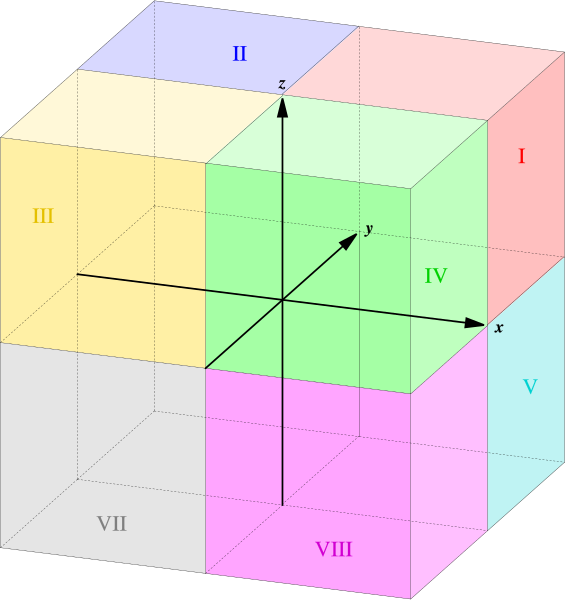
\includegraphics[width=0.4\textwidth]{chapters/chp1_pics/octant.png}
\caption{\textit{The eight octants of a three-dimensional Cartesian plot.}}
\label{fig:steinmetz}
\end{figure}

\subsection*{Toward Higher Dimensions: Imagining Four-Dimensional Space}

\noindent Extending to a fourth spatial dimension—though challenging to visualize—invites us to think beyond our physical intuition. In a four-dimensional space, each point is represented by an ordered quadruple \( (x, y, z, w) \), where \( w \) denotes the fourth dimension. Though difficult to imagine, one can think of \( w \) as adding an additional degree of freedom beyond our typical three-dimensional experience. Mathematicians and physicists work in four-dimensional (and higher-dimensional) spaces when dealing with complex phenomena, such as in the study of spacetime in general relativity. \\ \\ A helpful analogy is to consider how three-dimensional objects can cast two-dimensional shadows. In the same way, a four-dimensional object, known as a tesseract or hypercube, could project a three-dimensional “shadow.” This shadow could show us a trace of four-dimensional interactions, allowing us to infer properties of the higher dimension. While our intuition may falter beyond three dimensions, mathematical models provide structure. Calculations in higher-dimensional spaces can help solve problems in fields such as quantum mechanics and data science, where multi-dimensional datasets reveal patterns not visible in lower dimensions.





\subsection*{Distance and Midpoint Formulas in Three Dimensions} \index{Metric Formulas}

The distance and midpoint formulas in three-dimensional space are extensions of the two-dimensional formulas, derived from the Pythagorean Theorem. By understanding these derivations, we gain insight into the geometry of space and the relationships between points in three dimensions.

\subsubsection*{Derivation of the Distance Formula}

The distance formula in geometry is a direct extension of the Pythagorean Theorem, which states that for a right triangle with legs \( a \) and \( b \), and hypotenuse \( c \), the relationship between the sides is $a^2 + b^2 = c^2.$ We rearrange this equation for the hypotenuse to get $c = \sqrt{a^2 + b^2}$ This formula gives the length of the hypotenuse when the lengths of the other two sides are known. Now, consider finding the distance between two points \( P_1(x_1, y_1) \) and \( P_2(x_2, y_2) \) in a two-dimensional plane. To derive this distance, we construct a right triangle by taking the horizontal and vertical distances between these points:
\[
a = x_2 - x_1 \quad \text{and} \quad b = y_2 - y_1.
\]

\noindent Substituting \( a \) and \( b \) into the Pythagorean Theorem, we get:
\[
(x_2 - x_1)^2 + (y_2 - y_1)^2 = d^2,
\]
where \( d \) represents the distance between \( P_1 \) and \( P_2 \). Solving for \( d \) gives us the two-dimensional distance formula:
\[
d = \sqrt{(x_2 - x_1)^2 + (y_2 - y_1)^2}.
\]

\subsubsection*{Extending the Distance Formula to Three Dimensions}

To generalize this result to three-dimensional space, we need to consider an additional dimension, the \( z \)-axis. Given two points \( P_1(x_1, y_1, z_1) \) and \( P_2(x_2, y_2, z_2) \), the change in the \( z \)-direction introduces an additional ``side” in the Pythagorean relationship. Now, we have three differences:
\[
a = x_2 - x_1, \quad b = y_2 - y_1, \quad \text{and} \quad c = z_2 - z_1.
\]
\noindent We follow the same logic as before to obtain
\[
d = \sqrt{(x_2 - x_1)^2 + (y_2 - y_1)^2 + (z_2 - z_1)^2}.
\]

\noindent This formula allows us to calculate the straight-line distance between any two points in three-dimensional space by considering the differences along each of the three axes. Notice, that because of the square terms, the distance will always be positive or zero. Since we saw that for the Pythagorean theorem all we had to do to increase the dimensionality was include one more square term,  let's do that $n$-many times to go to any $n$th dimension we desire. Thus we obtain for any $n$-dimension we have
\[
d = \left(\sum_{j=1}^{n} \left(y_j - x_j\right)^2 \right)^{1/2} = \left((y_1 - x_1)^2 + \cdots + (y_n - x_n)^2\right)^{1/2}
\]

\subsubsection*{Midpoint Formula}
Similarly, the midpoint formula in three dimensions is derived from averaging the coordinates of the endpoints. For points \( P_1(x_1, y_1, z_1) \) and \( P_2(x_2, y_2, z_2) \), the midpoint \( M \) of the line segment joining \( P_1 \) and \( P_2 \) is given by:
\[
M = \left( \frac{x_1 + x_2}{2}, \frac{y_1 + y_2}{2}, \frac{z_1 + z_2}{2} \right).
\]
This midpoint divides the line segment into two equal halves, allowing us to locate the center point between \( P_1 \) and \( P_2 \) in three-dimensional space.


\exampleline
\begin{example}
A drone starts at point \( P_1 \) with coordinates \( (2, 3, 5) \) and needs to reach a target at point \( P_2 \) located at \( (7, 1, 10) \). Find the straight-line distance the drone needs to travel to reach the target.

\begin{solution}
To calculate the straight-line distance between points \( P_1(2, 3, 5) \) and \( P_2(7, 1, 10) \) in three-dimensional space, we apply the distance formula:
\[
d = \sqrt{(x_2 - x_1)^2 + (y_2 - y_1)^2 + (z_2 - z_1)^2}
\]

\begin{enumerate}
    \item Identify the coordinates:
    \[
    P_1(x_1, y_1, z_1) = (2, 3, 5), \quad P_2(x_2, y_2, z_2) = (7, 1, 10)
    \]

    \item Substitute the coordinates into the distance formula:
    \[
    d = \sqrt{(7 - 2)^2 + (1 - 3)^2 + (10 - 5)^2}
    \]

    \item Calculate each component:
    \begin{align*}
    (x_2 - x_1)^2 &= (7 - 2)^2 = 5^2 = 25 \\
    (y_2 - y_1)^2 &= (1 - 3)^2 = (-2)^2 = 4 \\
    (z_2 - z_1)^2 &= (10 - 5)^2 = 5^2 = 25
    \end{align*}

    \item Sum the components and take the square root:
    \[
    d = \sqrt{25 + 4 + 25} = \sqrt{54} = 3\sqrt{6} \approx 7.35
    \]

\end{enumerate}

Thus, the drone must travel approximately \( 7.35 \) units to reach its target.

\end{solution}
\end{example}
\exampleline



\subsection*{Introduction to Polar Coordinates}  \index{Polar Coordinates}

Polar coordinates provide an alternative way to describe points in a plane using a distance and an angle relative to a central point, typically the origin. The term “polar” is derived from the Latin word \textit{polus}, meaning “axis” or “pivot point,” indicating how this coordinate system revolves around a single fixed point as its central reference. In polar coordinates, each point is represented by an ordered pair \( (r, \theta) \), where:
\begin{itemize}
    \item \( r \): The radial distance from the origin (the straight-line distance from the point to the central origin).
    \item \( \theta \): The angular direction, measured from the positive \( x \)-axis, typically in degrees or radians, representing the angle at which the point is located relative to the origin.
\end{itemize}

\noindent Polar coordinates are particularly useful in situations involving circular or radial motion, such as describing points that orbit around a center. For instance, when an airplane travels in a curved path from one location to another, rectangular coordinates (i.e., \( x \) and \( y \)) may be inefficient, as they do not inherently account for direction and distance from a central point. Instead, polar coordinates allow the airplane’s position to be easily expressed in terms of distance and angle relative to the origin or any central reference, simplifying navigation, particularly over long distances along curved paths, such as on the Earth's surface.

\subsubsection*{Conversion Between Rectangular and Polar Coordinates}

The conversion between rectangular and polar coordinates relies on the Pythagorean Theorem and trigonometric relationships. Given a point \( (x, y) \) in rectangular coordinates:
\begin{itemize}
    \item The distance \( r \), from the origin to the point, can be derived using the Pythagorean Theorem:
    \[
    r = \sqrt{x^2 + y^2}
    \]
    \item The angle \( \theta \), representing the direction from the positive \( x \)-axis, is found using trigonometry:
    \[
    \theta = \tan^{-1} \left( \frac{y}{x} \right)
    \]
\end{itemize}

To convert back from polar to rectangular coordinates:
\begin{itemize}
    \item The \( x \)-coordinate can be found using:
    \[
    x = r \cos \theta
    \]
    \item The \( y \)-coordinate can be found using:
    \[
    y = r \sin \theta
    \]
\end{itemize}

\noindent To illustrate the difference between rectangular and polar coordinates, let’s examine the point \( (3, 4) \) in both systems. In rectangular coordinates, the point \( (3, 4) \) represents a location 3 units along the \( x \)-axis and 4 units along the \( y \)-axis. To express this point in polar coordinates, we calculate \( r \) and \( \theta \) as follows:

\[
r = \sqrt{3^2 + 4^2} = \sqrt{9 + 16} = \sqrt{25} = 5
\]
\[
\theta = \tan^{-1} \left( \frac{4}{3} \right) \approx 53.13^\circ
\]

\noindent Thus, the point \( (3, 4) \) in rectangular coordinates is equivalent to \( (5, 53.13^\circ) \) in polar coordinates. The following plot demonstrates both coordinate systems for this point. Rectangular coordinates \( (x, y) \) are shown on the standard Cartesian grid, while polar coordinates \( (r, \theta) \) use circles centered at the origin and rays extending out at different angles.

\begin{figure}[H]
    \centering
    \begin{tikzpicture}[scale=0.8]
        % Draw rectangular grid
        \foreach \x in {-4,-3,-2,-1,1,2,3,4}
            \draw[gray, thin] (\x, -4) -- (\x, 4);
        \foreach \y in {-4,-3,-2,-1,1,2,3,4}
            \draw[gray, thin] (-4, \y) -- (4, \y);

        % Draw polar circles
        \foreach \r in {1,2,3,4}
            \draw[gray, thin] (0,0) circle (\r);

        % Draw polar rays
        \foreach \a in {0,30,60,90,120,150,180,210,240,270,300,330}
            \draw[gray, thin] (0,0) -- (\a:4.5);

        % Label axes
        \draw[thick,->] (-4.5, 0) -- (4.5, 0) node[right] {$x$-axis};
        \draw[thick,->] (0, -4.5) -- (0, 4.5) node[above] {$y$-axis};

        % Plot the point in rectangular coordinates
        \filldraw[black] (3, 4) circle (3pt);

        % Plot the point in polar coordinates (5 units at 53.13 degrees)
        \draw[->, red, thick] (0,0) -- (53.13:5);

        % Blue arrows to show steps reaching (3, 4) along x- and y-axes
        \draw[->, blue, thick] (0, 0) -- (3, 0); % Arrow along x-axis
        \draw[->, blue, thick] (3, 0) -- (3, 4); % Arrow along y-axis

        % Add centered legend at the bottom
        \begin{scope}[shift={(-4, -5.5)}] % Center legend by adjusting x-position in shift
            \draw[thick, blue, ->] (0, 0) -- (1, 0) node[anchor=west] {Path in Rectangular Coordinates};
            \draw[thick, red, ->] (0, -0.5) -- (1, -0.5) node[anchor=west] {Path in Polar Coordinates};
        \end{scope}

    \end{tikzpicture}
    \caption{\textit{Plot showing both Rectangular and Polar representations of the point \( (3, 4) \) with a legend for coordinate paths.}}
    \label{fig:polar_rectangular_plot}
\end{figure}


\subsection*{Cylindrical Coordinates} \index{Cylindrical Coordinates}

The cylindrical coordinate system is an extension of polar coordinates, adding a vertical \( z \)-dimension to describe points in three-dimensional space. It is particularly useful for representing objects with circular symmetry around an axis, such as cylinders, tubes, and circular regions extending along a vertical axis. In cylindrical coordinates, each point is represented by \( (r, \theta, z) \), where:
\begin{itemize}
    \item \( r \): The radial distance from the \( z \)-axis, which is the distance from the point to the \( z \)-axis in the \( xy \)-plane.
    \item \( \theta \): The angle measured from the positive \( x \)-axis within the \( xy \)-plane, in radians, describing the angular position around the \( z \)-axis.
    \item \( z \): The vertical distance from the \( xy \)-plane, equivalent to the \( z \)-coordinate in rectangular coordinates, indicating height or depth.
\end{itemize}

\noindent In essence, cylindrical coordinates generalize polar coordinates by incorporating an additional \( z \)-coordinate, allowing us to describe points in three-dimensional space while maintaining the circular symmetry of polar coordinates around a central axis. If we set \( z = 0 \), cylindrical coordinates reduce to polar coordinates in the \( xy \)-plane, where a point is solely described by its distance \( r \) from the origin and the angle \( \theta \). 

\begin{figure}[H]
    \centering
% Set up the main coordinates for a 3D perspective
\tdplotsetmaincoords{65}{140}

\begin{tikzpicture}[scale=5, tdplot_main_coords]

% Define the radius and z-coordinate
\pgfmathsetmacro{\r}{0.8} % radius
\pgfmathsetmacro{\z}{0.7} % z-coordinate

% Use placeholders for x and y using angle theta
\draw[->, thick] (0,0,0) -- (1.2,0,0) node[anchor=west] {$x$-axis};
\draw[->, thick] (0,0,0) -- (0,1.2,0) node[anchor=west] {$y$-axis};
\draw[->, thick] (0,0,0) -- (0,0,1.2) node[anchor=south] {$z$-axis};

% Draw the vector in cylindrical coordinates
\draw[->, blue!70!black, ultra thick] (0,0,0) -- ({\r*cos(30)},{\r*sin(30)},\z) node[anchor=south] {$(r, \theta, z)$};

% Project to xy-plane
\draw[dashed, blue!50] ({\r*cos(30)},{\r*sin(30)},\z) -- ({\r*cos(30)},{\r*sin(30)},0);
\draw[dashed, blue!50] ({\r*cos(30)},{\r*sin(30)},0) -- (0, 0, 0);

% Draw the circle in the xy-plane to represent radius
\draw[thick, dashed, gray] (0,0,0) circle (\r);

% Draw an arc to indicate the angle theta
\draw[thick, ->, red!70] (0.6,0) arc[start angle=0, end angle=30, radius=0.6];
\node[anchor=west] at (0.35,0.05) {$\theta$};

% Projection points and labels
\filldraw[blue!50] ({\r*cos(30)},{\r*sin(30)},0) circle (0.5pt) node[anchor=north east] {$(r, \theta, 0)$};
\filldraw[blue!50] ({\r*cos(30)},{\r*sin(30)},\z) circle (0.5pt);

% Radius label
\draw[thick, dashed, green!70!black] (0,0,0) -- ({\r*cos(30)},{\r*sin(30)},0);
\node[anchor=north east] at ({\r*cos(15)/2},{\r*sin(15)/2},0) {$r$};

\end{tikzpicture}

    \caption{\textit{A point in three-dimensional space represented in cylindrical coordinates \( (r, \theta, z) \). The radius \( r \) is the distance from the \( z \)-axis, \( \theta \) is the angle measured from the positive \( x \)-axis, and \( z \) is the vertical coordinate.}}
    \label{fig:cylindrical_point_symbolic}
\end{figure}



\noindent Cylindrical coordinates are widely used in fields like physics and engineering where problems often exhibit cylindrical or rotational symmetry. For instance, in analyzing magnetic fields around a wire, fluid flow in pipes, or any phenomenon with a circular base extending along a vertical dimension, cylindrical coordinates provide a natural and efficient way to describe the system.

\subsubsection*{Converting Between Cylindrical and Rectangular Coordinates:}
To switch between cylindrical and rectangular coordinates, we use trigonometric relationships similar to those in polar coordinates, with the \( z \)-coordinate remaining consistent between both systems.

\begin{itemize}
    \item To convert from cylindrical \( (r, \theta, z) \) to rectangular \( (x, y, z) \):
    \[
    x = r \cos \theta, \quad y = r \sin \theta, \quad z = z
    \]
    This transformation projects the point \( (r, \theta) \) in the \( xy \)-plane into \( x \)- and \( y \)-coordinates using trigonometry, while \( z \) remains unchanged.

    \item To convert from rectangular \( (x, y, z) \) to cylindrical \( (r, \theta, z) \):
    \[
    r = \sqrt{x^2 + y^2}, \quad \theta = \tan^{-1} \left( \frac{y}{x} \right), \quad z = z
    \]
    Here, \( r \) is calculated as the distance from the point to the \( z \)-axis (similar to the Pythagorean distance in polar coordinates), and \( \theta \) is the angle around the \( z \)-axis. The \( z \)-coordinate remains the same in both representations.
\end{itemize}

\noindent This conversion framework allows easy switching between cylindrical and rectangular coordinates depending on the symmetry and nature of the problem at hand. In problems with circular symmetry along an axis, cylindrical coordinates simplify analysis and calculation by leveraging the radial and angular structure inherent to the system.


\subsection*{Spherical Coordinates} \index{Spherical Coordinates}

Spherical coordinates are ideal for problems with radial symmetry, such as those involving spheres or radial fields. Each point in spherical coordinates is represented by \( (\rho, \theta, \phi) \):
\begin{itemize}
    \item \( \rho \): The radial distance from the origin (distance from the point to the origin).
    \item \( \theta \): The angle in the \( xy \)-plane from the positive \( x \)-axis, measured counterclockwise.
    \item \( \phi \): The angle between the point and the positive \( z \)-axis (measured from the \( z \)-axis downward).
\end{itemize}

\noindent Spherical coordinates are particularly useful for scenarios where an object moves in a circular arc around a central point and has varying elevation, such as a planet orbiting a star, a camera with full rotation, or a baseball bat’s swing through the air. When a softball player swings a bat to hit a ball, the bat moves in a curved, sweeping motion around the player. The motion of the bat can be best described in spherical coordinates:
\begin{itemize}
    \item Radial Distance (\( \rho \)): The distance of the bat’s tip from the player’s body (the origin) varies, allowing for control over how close or far the bat reaches.
    \item Horizontal Angle (\( \theta \)): The angle \( \theta \) in the \( xy \)-plane represents the circular path of the bat around the player as they swing.
    \item Vertical Angle (\( \phi \)): The vertical angle \( \phi \) describes how high or low the bat is swung, which varies depending on whether the player adjusts to hit a high or low pitch.
\end{itemize}

\begin{figure}[H]
    \centering
\tdplotsetmaincoords{60}{110}
%
\pgfmathsetmacro{\rvec}{.8}
\pgfmathsetmacro{\thetavec}{30}
\pgfmathsetmacro{\phivec}{60}
%
\begin{tikzpicture}[scale=5,tdplot_main_coords]
    \coordinate (O) at (0,0,0);
    \draw[thick,->] (0,0,0) -- (1,0,0) node[anchor=north east]{$x$};
    \draw[thick,->] (0,0,0) -- (0,1,0) node[anchor=north west]{$y$};
\draw[thick,->] (0,0,0) -- (0,0,1) node[anchor=south]{$z$};
    \tdplotsetcoord{P}{\rvec}{\thetavec}{\phivec}
    \draw[-stealth,color=red] (O) -- (P) node[above right] {$\rho$};
    \draw[dashed, color=red] (O) -- (Pxy);
    \draw[dashed, color=red] (P) -- (Pxy);
    \tdplotdrawarc{(O)}{0.2}{0}{\phivec}{anchor=north}{$\phi$}
    \tdplotsetthetaplanecoords{\phivec}
    \tdplotdrawarc[tdplot_rotated_coords]{(0,0,0)}{0.5}{0}%
        {\thetavec}{anchor=south west}{$\theta$}


\end{tikzpicture}
\caption{\textit{A representation of the spherical coordinate system.}}
\end{figure}


\noindent Unlike cylindrical coordinates, which would only capture the horizontal rotation around a central vertical axis (the player’s body), spherical coordinates provide a complete representation of the bat’s path, including its height and depth relative to the player’s position. Thus, spherical coordinates offer a more accurate and flexible framework for capturing the full 3D motion of a softball swing.

\begin{figure}[H]
    \centering
    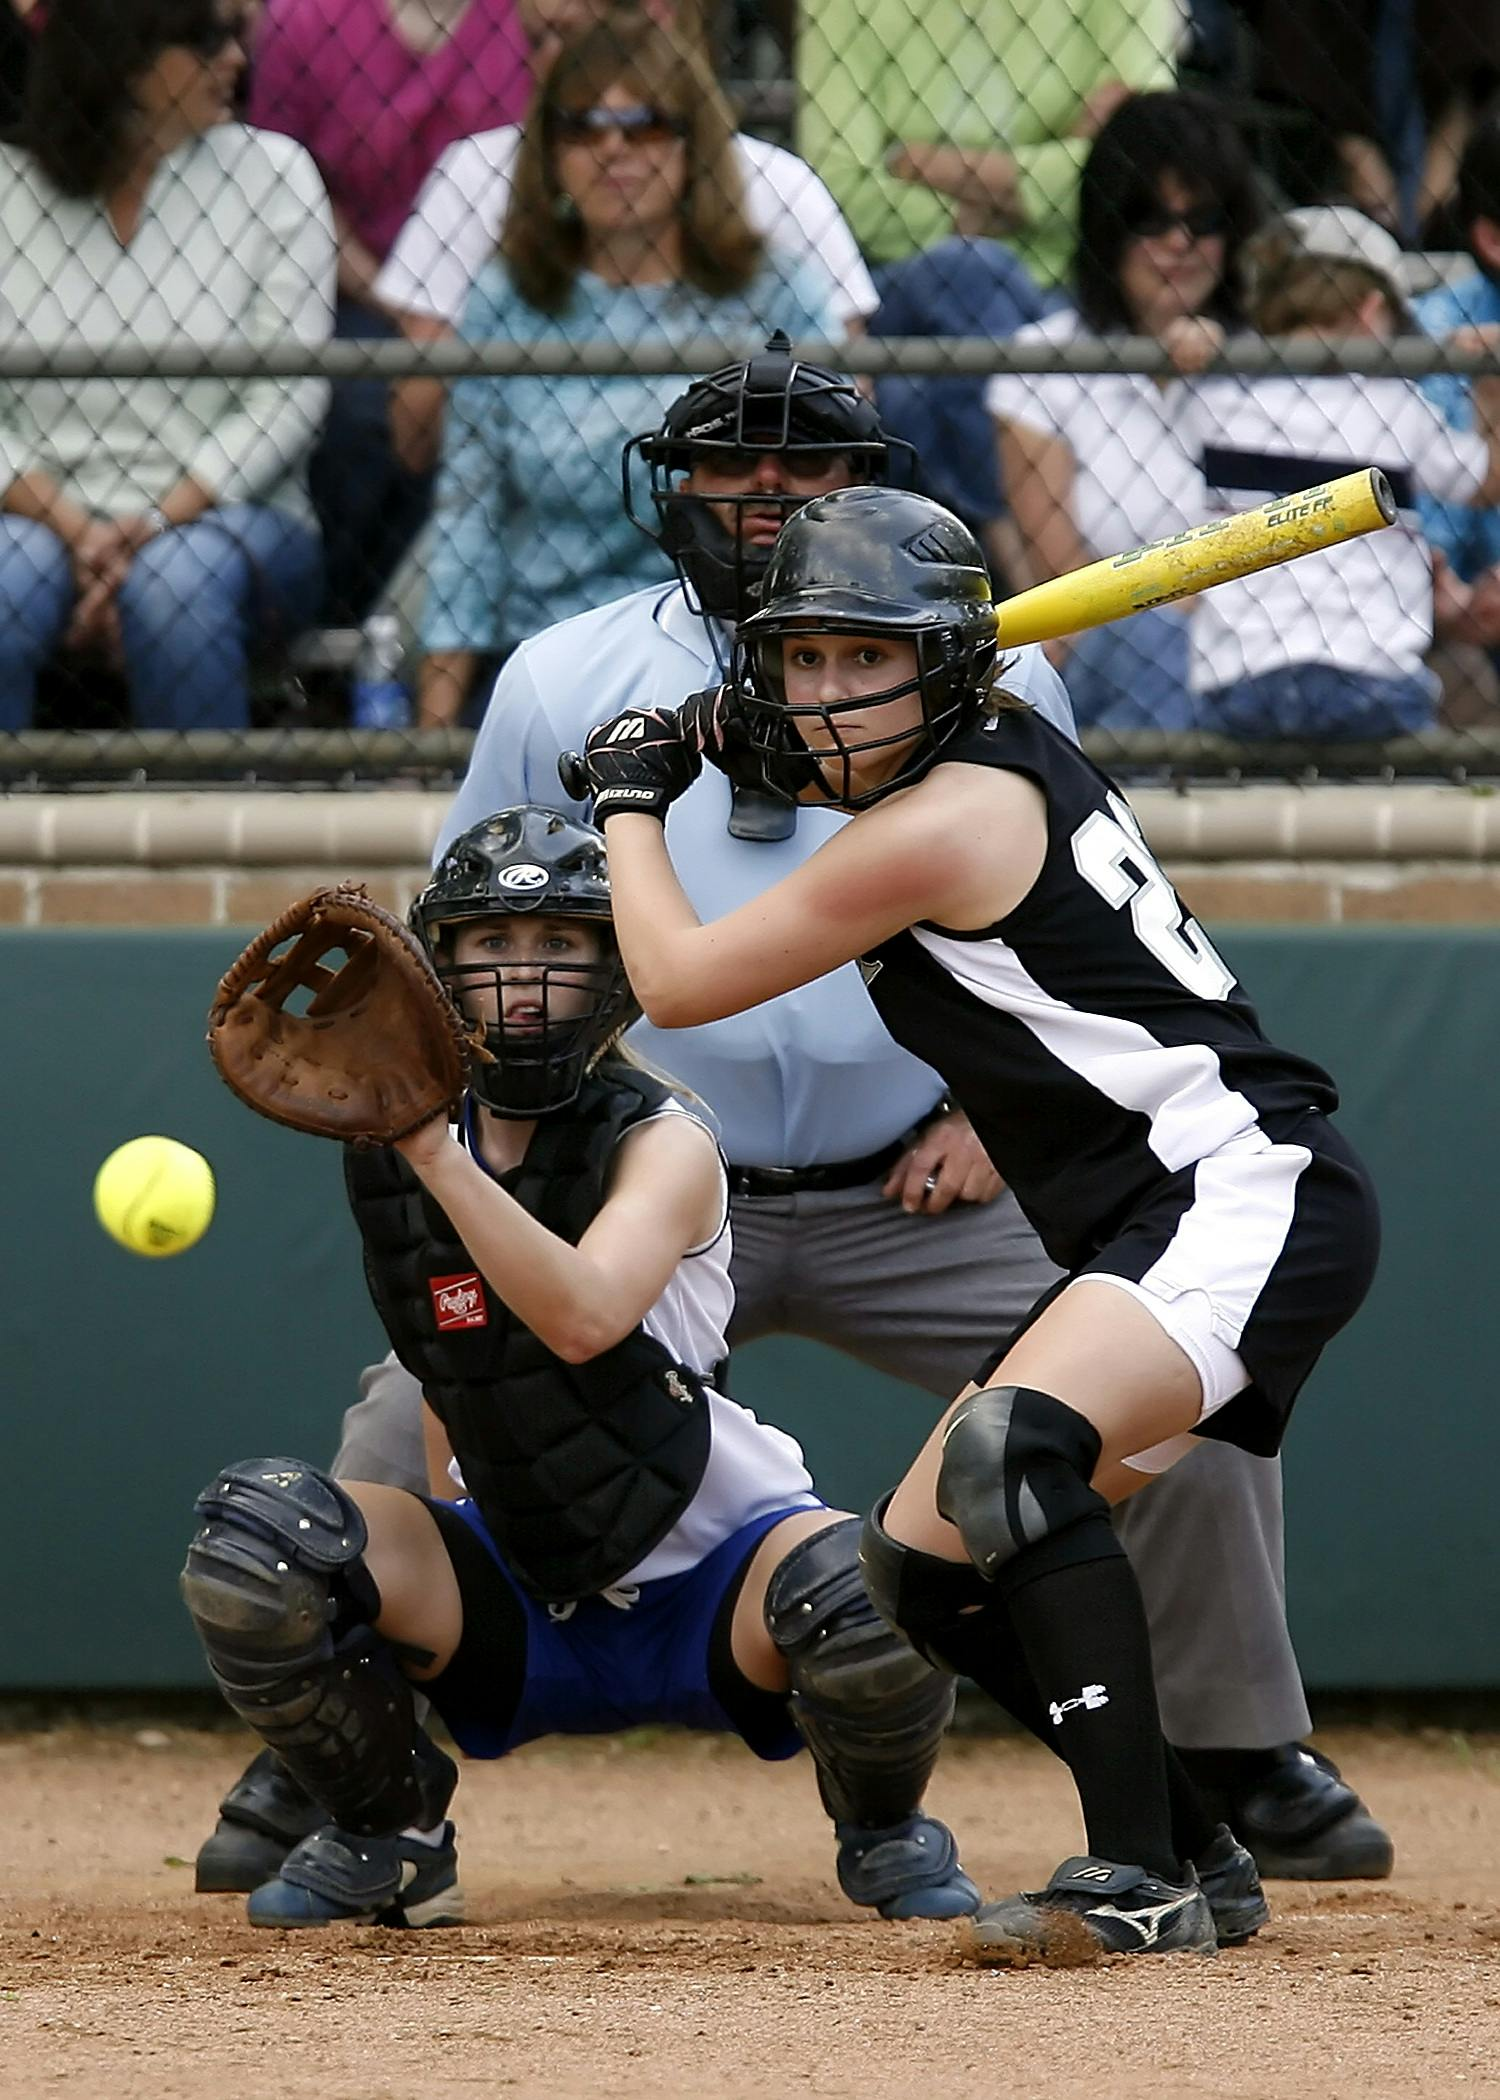
\includegraphics[width=0.3\textwidth]{chapters/chp1_pics/softball.jpg}
    \caption{\textit{A softball swing is best represented in spherical coordinates, capturing the radial distance, horizontal angle, and vertical angle of the bat's position relative to the player.}}
    \label{fig:softball_swing}
\end{figure}

\subsubsection{Converting Between Spherical and Rectangular Coordinates:}
\begin{itemize}
    \item To convert from spherical \( (\rho, \theta, \phi) \) to rectangular \( (x, y, z) \):
    \[
    x = \rho \sin \phi \cos \theta, \quad y = \rho \sin \phi \sin \theta, \quad z = \rho \cos \phi
    \]
    \item To convert from rectangular \( (x, y, z) \) to spherical \( (\rho, \theta, \phi) \):
    \[
    \rho = \sqrt{x^2 + y^2 + z^2}, \quad \theta = \tan^{-1} \left( \frac{y}{x} \right), \quad \phi = \cos^{-1} \left( \frac{z}{\rho} \right)
    \]
\end{itemize}


\exampleline
\begin{example}
A bird is flying along a circular path around a radio tower, while also increasing its altitude. At a certain moment, the bird’s position relative to the tower is given by the cylindrical coordinates \( (r, \theta, z) = (100, \frac{\pi}{4}, 50) \), where \( r \) is in meters and \( z \) represents height. Convert this position into rectangular coordinates to determine the bird’s \( (x, y, z) \) coordinates in the 3D plane.

\begin{solution}
To convert from cylindrical coordinates \( (r, \theta, z) \) to rectangular coordinates \( (x, y, z) \), we use the following conversion formulas:
\[
x = r \cos \theta, \quad y = r \sin \theta, \quad z = z
\]

Given:
\[
r = 100, \quad \theta = \frac{\pi}{4}, \quad z = 50
\]

\begin{enumerate}
    \item Calculate \( x \):
    \[
    x = 100 \cos \frac{\pi}{4} = 100 \cdot \frac{\sqrt{2}}{2} = 50 \sqrt{2}
    \]

    \item Calculate \( y \):
    \[
    y = 100 \sin \frac{\pi}{4} = 100 \cdot \frac{\sqrt{2}}{2} = 50 \sqrt{2}
    \]

    \item The \( z \)-coordinate remains the same:
    \[
    z = 50
    \]

    \item Therefore, the rectangular coordinates of the bird’s position are:
    \[
    (x, y, z) = \left( 50 \sqrt{2}, 50 \sqrt{2}, 50 \right)
    \]
\end{enumerate}

\end{solution}
\end{example}
\exampleline
\begin{example}
In an automated car assembly plant, a spherical robotic arm is used to position car parts in 3D space. The arm operates by extending its length, rotating horizontally, and pivoting vertically. At a certain moment, the robotic arm performs the following actions:

\begin{itemize}
    \item Extends to a length of 2 meters.
    \item Rotates \( 60^\circ \) counterclockwise from the positive \( x \)-axis.
    \item Raises the arm \( 45^\circ \) above the horizontal plane.
\end{itemize}

\noindent Identify which spherical coordinate (\( \rho \), \( \theta \), or \( \phi \)) corresponds to each action, and write down the spherical coordinates of the arm's end effector after this movement.

\begin{solution}
In spherical coordinates:
\begin{itemize}
    \item \( \rho \) represents the distance from the origin to the point (length of the arm).
    \item \( \theta \) is the angle measured in the \( xy \)-plane from the positive \( x \)-axis (horizontal rotation).
    \item \( \phi \) is the angle measured from the positive \( z \)-axis down to the point (vertical angle).
\end{itemize}

Given the actions:

\begin{enumerate}
    \item \textbf{Extension to a length of 2 meters}:
        \begin{itemize}
            \item This corresponds to \( \rho = 2 \, \text{m} \).
        \end{itemize}

    \item \textbf{Rotation \( 60^\circ \) counterclockwise from the positive \( x \)-axis}:
        \begin{itemize}
            \item This corresponds to \( \theta = 60^\circ \) or \( \theta = \dfrac{\pi}{3} \, \text{radians} \).
        \end{itemize}

    \item \textbf{Raising the arm \( 45^\circ \) above the horizontal plane}:
        \begin{itemize}
            \item Since \( \phi \) is measured from the positive \( z \)-axis downwards, we need to calculate \( \phi \).
            \item The horizontal plane corresponds to \( \phi = 90^\circ \) (as it is \( 90^\circ \) down from the positive \( z \)-axis).
            \item Raising the arm \( 45^\circ \) above the horizontal plane means the angle from the positive \( z \)-axis is:
            \[
            \phi = 90^\circ - 45^\circ = 45^\circ \quad \text{or} \quad \phi = \dfrac{\pi}{4} \, \text{radians}.
            \]
        \end{itemize}
\end{enumerate}

\end{solution}
\end{example}
\exampleline

\subsection*{Choice of Coordinates}

The choice of coordinate system is essential in simplifying calculations and providing clarity in solving problems. Each coordinate system has advantages depending on the problem's geometry, symmetry, and underlying physical properties. Below is a comparison of when each system is most useful.

\begin{itemize}
    \item \textbf{Rectangular (Cartesian) Coordinates:} 
    In rectangular coordinates, each point is specified by its perpendicular distances from the \( x \)-, \( y \)-, and \( z \)-axes. This system is intuitive and ideal for objects and problems aligned along the three principal axes, such as rectangular prisms, planes, and many engineering structures.
    \item \textbf{Polar Coordinates:}
    Polar coordinates are well-suited for two-dimensional problems involving circular or rotational symmetry around a central point. Problems that naturally involve rotation or radial symmetry—such as the motion of a particle in a circular path or objects positioned relative to a central point—benefit from polar coordinates.

    \item \textbf{Cylindrical Coordinates:} 
    Cylindrical coordinates are an extension of polar coordinates into three dimensions, making them ideal for problems with circular symmetry around a central vertical axis, such as cylindrical objects or fields surrounding a wire. For example, fluid flow in a pipe, magnetic fields around a wire, or the structure of a cylindrical tank are best analyzed using cylindrical coordinates.

    \item \textbf{Spherical Coordinates:} 
    Spherical coordinates extend the idea of radial symmetry into three dimensions and are best suited for objects and fields with a spherical or radial symmetry, such as planets, stars, and electric fields radiating from a point charge.
\end{itemize}




\newpage


\lecture{Vectors} \index{Vectors}

\noindent In progressing from two-dimensional space to three-dimensional space, vectors become an essential concept for describing both position and direction. Vectors allow us to represent not only points but also the direction and magnitude of movement or force in space, forming the basis for advanced topics in calculus.

\subsection*{Definition of Vectors}

\noindent As we move from two-dimensional space into three dimensions, vectors become crucial for describing both position and direction. Vectors aren’t just about marking a location—they let us describe how something moves or acts, combining both its size (magnitude) and direction. This combination of information forms the basis of advanced ideas in calculus, physics, and engineering. For instance, knowing the strength of a wind gust without knowing the direction isn’t very helpful. But by representing it as a vector, we gain both its intensity and the path it follows. \\ \\ We represent a vector in three-dimensional space with an ordered triple \( \mathbf{v} =\langle v_x, v_y, v_z \rangle \), where:
\begin{itemize}
    \item \( v_x \): Shows the vector’s reach along the \( x \)-axis.
    \item \( v_y \): Shows its reach along the \( y \)-axis.
    \item \( v_z \): Shows its reach along the \( z \)-axis.
\end{itemize}

\noindent Each component captures the vector’s effect along one axis, allowing it to describe anything with direction and magnitude. In addition to using \( \mathbf{v}\), we may also write \( \vec{v} \). This is typically what students write in their notebooks when indicating a vector. For listing components of a vector we may write either \( (v_x, v_y, v_z) \) or \( \langle v_x, v_y, v_z \rangle \). To eliminate ambiguity from describing points, we will use the latter notation. \\ \\ To make vectors more tangible, imagine them as arrows in space. Each arrow’s direction and length tell us the direction and strength of an action or movement—like the current in a river. At each point along the river, an arrow (or vector) can show how fast and in which direction the water flows. Vectors make it possible to describe these continuous, directed motions, making them ideal for representing physical forces or speeds in space. \\ \\ Vectors also have special properties that make them versatile tools. For example, they can be moved around in space without changing their meaning, a property called \textit{translational invariance}. This means a vector maintains its effect regardless of its starting point, allowing us to describe forces or velocities that act consistently no matter where they occur. They can also be ``stacked” or added together, which is essential in physics. For example, if two people push a box from different directions, the net effect on the box’s movement can be represented by the sum of their vectors. Vectors can also be scaled up or down, describing changes in strength or intensity. For example, if a car speeds up, its velocity vector is scaled up to reflect its increased speed while keeping the same direction. This operation, called \textit{scalar multiplication}, lets us adjust vectors without altering their paths.

\begin{figure}[H]
    \centering
% Set up the main coordinates for a 3D perspective, shifted slightly left
\tdplotsetmaincoords{65}{140}

\begin{tikzpicture}[scale=5, tdplot_main_coords]

% Define points for a vector in 3D
\pgfmathsetmacro{\vx}{0.6}
\pgfmathsetmacro{\vy}{0.5}
\pgfmathsetmacro{\vz}{0.7}

% Draw axes
\draw[->, thick] (0,0,0) -- (1.2,0,0) node[anchor=west] {$x$-axis};
\draw[->, thick] (0,0,0) -- (0,1.2,0) node[anchor=west] {$y$-axis};
\draw[->, thick] (0,0,0) -- (0,0,1.2) node[anchor=south] {$z$-axis};

% Draw the main vector from the origin to (vx, vy, vz)
\draw[->, blue!70!black, ultra thick] (0,0,0) -- (\vx,\vy,\vz) node[anchor=south] {$(x, y, z)$};

% Project dashed lines to each coordinate plane
\draw[dashed, blue!50] (\vx, \vy, \vz) -- (\vx, \vy, 0);  % xy-plane
\draw[dashed, blue!50] (\vx, \vy, \vz) -- (\vx, 0, \vz);  % xz-plane
\draw[dashed, blue!50] (\vx, \vy, \vz) -- (0, \vy, \vz);  % yz-plane

% Projection points
\filldraw[blue!50] (\vx, \vy, 0) circle (0.5pt);
\filldraw[blue!50] (\vx, 0, \vz) circle (0.5pt);
\filldraw[blue!50] (0, \vy, \vz) circle (0.5pt);

\end{tikzpicture}

    \caption{\textit{A vector in three-dimensional space represented by components along \( x \), \( y \), and \( z \) axes.}}
    \label{fig:3d_vector}
\end{figure}


\subsection*{Vector Magnitude and Direction}

\noindent The \textit{magnitude} or \textit{length} of a vector \( \mathbf{v} = \langle v_x, v_y, v_z \rangle \) is denoted by \( |\mathbf{v}| \) (and in some advanced texts as \( \| \mathbf{v} \| \)) and is calculated by using the Pythagorean theorem extended to three dimensions. This is because each component of the vector \( v_x \), \( v_y \), and \( v_z \) represents the vector’s ``reach” along the \( x \)-, \( y \)-, and \( z \)-axes. The magnitude formula is directly related to the distance formula covered previously:
\[
|\mathbf{v}| = \sqrt{v_x^2 + v_y^2 + v_z^2}.
\]

\noindent For example, if \( \mathbf{v} = (3, -4, 12) \), then:
\[
|\mathbf{v}| = \sqrt{3^2 + (-4)^2 + 12^2} = \sqrt{9 + 16 + 144} = \sqrt{169} = 13.
\]

\noindent The magnitude provides a sense of ``how much” or ``how far” the vector reaches in space, without giving any indication of direction. With magnitude, we gain a crucial part of the vector’s identity, as it represents the scale or intensity of whatever the vector is describing—such as the speed of a moving object or the strength of a force.

\subsubsection*{Unit Vectors and Direction Cosines}

\noindent A \textit{unit vector} is a vector that has been scaled to have a magnitude of exactly 1 while keeping its direction unchanged. Unit vectors serve as pure directional indicators, providing only the direction without any size or scale. They are especially useful for defining the principal directions along each axis in three-dimensional space. In three-dimensional space, we define the standard unit vectors along the \( x \)-, \( y \)-, and \( z \)-axes as:
\[
\mathbf{i} = \langle 1, 0, 0 \rangle, \quad \mathbf{j} = \langle 0, 1, 0 \rangle, \quad \mathbf{k} = \langle0, 0, 1 \rangle.
\]
\noindent These vectors—\( \mathbf{i} \), \( \mathbf{j} \), and \( \mathbf{k} \)—represent the directions along each principal axis with a magnitude of 1, making them ideal for constructing and breaking down other vectors. In other texts you may also see them written as \( \mathbf{\hat{i}} \), \( \mathbf{\hat{j}} \), and \( \mathbf{\hat{k}} \). Typically important unit vectors are also written this way with a hat. Any vector \( \mathbf{v} = \langle v_x, v_y, v_z \rangle \) can be written in terms of \( \mathbf{i} \), \( \mathbf{j} \), and \( \mathbf{k} \) as:
\[
\mathbf{v} = v_x \mathbf{i} + v_y \mathbf{j} + v_z \mathbf{k}.
\]
\noindent Expressing vectors in this form allows us to separate and analyze their individual components along each axis, which simplifies many operations in vector algebra and physics. To create a unit vector \( \mathbf{u} \) that points in the same direction as a given vector \( \mathbf{v} \), we divide \( \mathbf{v} \) by its magnitude \( |\mathbf{v}| \). For a vector \( \mathbf{v} = (v_x, v_y, v_z) \), the unit vector \( \mathbf{u} \) in the direction of \( \mathbf{v} \) is:
\[
\mathbf{u} = \frac{\mathbf{v}}{|\mathbf{v}|} = \left\langle \frac{v_x}{|\mathbf{v}|}, \frac{v_y}{|\mathbf{v}|}, \frac{v_z}{|\mathbf{v}|} \right\rangle.
\]


\noindent This process of scaling a vector to make it a unit vector is called \textit{normalization}. Normalization allows us to create a standardized version of any vector that preserves its direction while adjusting its magnitude to exactly 1. We will see normal vectors all over this entire study of multi-variable Calculus--more to be addressed about this soon. \\ \\ The concept of unit vectors is valuable in many applications because they give us a standardized way to indicate direction independently of magnitude. For instance, if we only care about the direction an object is moving (such as ``due north”) and not its speed, we can use a unit vector to represent that direction without indicating scale. \\ \\ \textbf{Direction cosines} \index{Direction Cosines} are another way to describe a vector’s direction, using trigonometric relationships to find the angles the vector makes with each coordinate axis. For a vector \( \mathbf{v} = \langle v_x, v_y, v_z \rangle \), direction cosines are the cosines of the angles \( \alpha \), \( \beta \), and \( \gamma \) that \( \mathbf{v} \) makes with the \( x \)-, \( y \)-, and \( z \)-axes, respectively. They are calculated by dividing each component of the vector by its magnitude, which corresponds to taking the cosine of each directional angle:
\[
\cos \alpha = \frac{v_x}{|\mathbf{v}|}, \quad \cos \beta = \frac{v_y}{|\mathbf{v}|}, \quad \cos \gamma = \frac{v_z}{|\mathbf{v}|}.
\]

\noindent The use of cosines here is rooted in trigonometry: when a vector is projected onto an axis, the cosine of the angle gives the ratio between the length of the projection (the component) and the length of the vector itself. This relationship provides a way to understand how the vector is oriented relative to each axis, which is essential in fields like physics and engineering, where precise direction often matters as much as magnitude.


\begin{figure}[H]
    \centering
    \begin{tikzpicture}
        % Draw axes
        \draw[thick,->] (-1,0) -- (5,0) node[right] {$x$-axis};
        \draw[thick,->] (0,-1) -- (0,4) node[above] {$y$-axis};
        
        % Draw vector v
        \draw[thick,->,blue] (0,0) -- (4,3) node[anchor=south west] {$\mathbf{v}$};

        % Project vector v onto x-axis
        \draw[dashed] (4,3) -- (4,0) node[anchor=north] {$v_x$};
        \draw[dashed] (4,3) -- (0,3) node[anchor=east] {$v_y$};

        % Label angle theta
        \draw[thick,->] (1,0) arc[start angle=0,end angle=36.87,radius=1] node[midway, right] {$\theta$};

        % Show magnitude of vector v with customizable position
        \node (magnitude) at (2.2,2) {$|\mathbf{v}|$}; % Moveable label

        % Optional: Add a label you can position manually
        % Uncomment and adjust coordinates to place $|\mathbf{v}|$ in a new location
        % \node at (custom_x, custom_y) {$|\mathbf{v}|$};
    \end{tikzpicture}
    \caption{\textit{A 2D vector \( \mathbf{v} \) showing the angle \( \theta \) with the \( x \)-axis. The direction cosine, \( \cos \theta \), is the ratio \( \frac{v_x}{|\mathbf{v}|} \), which describes the vector’s orientation relative to the \( x \)-axis.}}
    \label{fig:direction_cosines}
\end{figure}


\subsubsection*{Normal Vectors}

\noindent \noindent While direction cosines help us understand how a vector is oriented relative to our coordinate axes, we often need to describe vectors that are perpendicular to other vectors or surfaces. This leads us to the concept of normal vectors. \\

\noindent A \textit{normal vector} (or simply a \textit{normal}) is a vector $\mathbf{n}$ that is perpendicular to something else, like a line or a surface. Normal vectors are especially useful because many problems in physics and geometry involve perpendicular directions. For example, when light hits a mirror, we need to know the direction perpendicular to the mirror's surface to determine how the light will reflect. \\

\noindent For a line in two dimensions, if we know a vector along the line, we can find a normal vector by simply swapping its $x$ and $y$ components and making one of them negative. For example, if a vector along a line is \( \mathbf{v} = \langle 3, 4 \rangle \), then \( \mathbf{n} = \langle -4, 3 \rangle \) is a normal vector to that line. We can verify this is true because perpendicular vectors have components that, when multiplied and summed, equal zero: \( 3(-4) + 4(3) = -12 + 12 = 0 \). \\

\noindent  In polar coordinates, we can find normal vectors in a similar way. For instance, at any point on the circle where \( r = 1 \), a vector pointing outward from the circle (normal to the circle) has components \( \langle \cos\theta, \sin\theta \rangle \). You can visualize this by imagining the normal vector as pointing straight out from the circle at each point, like spokes on a wheel. \\




\noindent Just like any other vector, we can turn a normal vector into a unit normal vector by dividing by its length. Sometimes we denote this like our unit vectors $\mathbf{\hat{n}}$. For instance, in our first example:
\[
\mathbf{\hat{n}} = \frac{\langle -4, 3 \rangle}{\sqrt{(-4)^2 + 3^2}} = \frac{\langle -4, 3 \rangle}{5} = \left\langle -\frac{4}{5}, \frac{3}{5} \right\rangle.
\]

\noindent Unit normal vectors as we have seen are useful because they give us a standard way to describe perpendicular directions, regardless of the size of the original vectors we started with. We'll see many applications of normal vectors as we continue our study of vectors and their uses in geometry and physics.

\begin{figure}[H]
    \centering
    \begin{minipage}{0.48\textwidth}
        \centering
        \begin{tikzpicture}[scale=1]
            % Cartesian axes
            \draw[thick,->] (-2,0) -- (4,0) node[right] {$x$};
            \draw[thick,->] (0,-2) -- (0,4) node[above] {$y$};
            
            % Original vector
            \draw[thick,->,blue] (0,0) -- (3,2) node[anchor=west] {$\mathbf{v}$};
            
            % Normal vector (perpendicular)
            \draw[thick,->,red] (0,0) -- (-2,3) node[anchor=south] {$\mathbf{n}$};
           
            
        \end{tikzpicture}
        \caption*{(a) Normal vector in Cartesian coordinates}
    \end{minipage}
    \begin{minipage}{0.48\textwidth}
        \centering
        \begin{tikzpicture}[scale=1]
            % Draw the unit circle
            \draw[thick] (0,0) circle (2);
            
            % Axes
            \draw[thick,->] (-2.5,0) -- (2.5,0) node[right] {$x$};
            \draw[thick,->] (0,-2.5) -- (0,2.5) node[above] {$y$};
            
            % Point on circle at theta = pi/4
            \coordinate (P) at (45:2);
            
            % Radial vector (to point on circle)
            \draw[thick,->,blue] (0,0) -- (P) node[anchor=south west] {$\mathbf{r}$};
            
            % Normal vector (tangent to circle)
            \draw[thick,->,red] (P) -- ($(P)+(135:1.5)$) node[anchor=south] {$\mathbf{n}$};
            
            % Angle label
            \draw[thick] (0.5,0) arc (0:45:0.5) node[midway,above right] {$\theta$};
            
        \end{tikzpicture}
        \caption*{(b) Normal vector on a circle (polar)}
    \end{minipage}
    \caption{\textit{Normal vectors shown in different coordinate systems. In (a), the normal vector $\mathbf{n}$ is perpendicular to vector $\mathbf{v}$. In (b), the normal vector $\mathbf{n}$ is perpendicular to the radial vector $\mathbf{r}$ at a point on the circle.}}
    \label{fig:normal_vectors}
\end{figure}

\exampleline
\begin{example}
A heavy box is being pushed along a factory floor with a force vector \( \mathbf{F} = \langle 9, 12, 15 \rangle \) (measured in newtons) representing the components of the force applied along the \( x \)-, \( y \)-, and \( z \)-axes. Find the magnitude of \( \mathbf{F} \), determine the unit vector in the direction of \( \mathbf{F} \), calculate the direction cosines of \( \mathbf{F} \) with respect to each axis, and find a normal vector to \( \mathbf{F} \) that lies in the $xy$-plane.

\begin{solution}
To find the unit vector and direction cosines, we first need the magnitude of \( \mathbf{F} \).

\begin{enumerate}
    \item Calculate the magnitude \( |\mathbf{F}| \) using the formula:
    \[
    |\mathbf{F}| = \sqrt{F_x^2 + F_y^2 + F_z^2}
    \]
    Substitute \( F_x = 9 \), \( F_y = 12 \), and \( F_z = 15 \):
    \[
    |\mathbf{F}| = \sqrt{9^2 + 12^2 + 15^2} = \sqrt{81 + 144 + 225} = \sqrt{450} = 15\sqrt{2}
    \]

    \item Now, calculate the unit vector \( \mathbf{u} \) in the direction of \( \mathbf{F} \):
    \[
    \mathbf{u} = \frac{\mathbf{F}}{|\mathbf{F}|} = \left\langle \frac{9}{15\sqrt{2}}, \frac{12}{15\sqrt{2}}, \frac{15}{15\sqrt{2}} \right\rangle
    \]
    Simplify each component:
    \[
    \mathbf{u} = \left\langle \frac{3}{5\sqrt{2}}, \frac{4}{5\sqrt{2}}, \frac{1}{\sqrt{2}} \right\rangle
    \]

    \item Next, we calculate the direction cosines, which are the cosines of the angles that \( \mathbf{F} \) makes with each coordinate axis. These are given by:
    \[
    \cos \alpha = \frac{F_x}{|\mathbf{F}|}, \quad \cos \beta = \frac{F_y}{|\mathbf{F}|}, \quad \cos \gamma = \frac{F_z}{|\mathbf{F}|}
    \]
    
    Substitute the values of \( F_x \), \( F_y \), \( F_z \), and \( |\mathbf{F}| = 15\sqrt{2} \):
    \begin{align*}
        \cos \alpha &= \frac{9}{15\sqrt{2}} = \frac{3}{5\sqrt{2}} \\
        \cos \beta &= \frac{12}{15\sqrt{2}} = \frac{4}{5\sqrt{2}} \\
        \cos \gamma &= \frac{15}{15\sqrt{2}} = \frac{1}{\sqrt{2}}
    \end{align*}

\item Finally, let's find a normal vector to \( \mathbf{F} \) that lies in the $xy$-plane. We can do this by:
\begin{itemize}
    \item First, considering only the $x$ and $y$ components of \( \mathbf{F} \): \( \langle 9, 12 \rangle \)
    \item To find a normal vector in 2D, we can swap these components and make one negative: \( \langle -12, 9 \rangle \)
    \item Since we want this normal vector in 3D space lying in the xy-plane, we add a $z$-component of $0$
\end{itemize}
Therefore, one possible normal vector is \( \mathbf{n} = \langle -12, 9, 0 \rangle \).

We can verify this is indeed perpendicular to \( \mathbf{F} \) by checking if their dot product is zero:
\[
\mathbf{F} \cdot \mathbf{n} = 9(-12) + 12(9) + 15(0) = -108 + 108 + 0 = 0
\]

\item Therefore, our complete results are:
\begin{itemize}
\item The magnitude of \( \mathbf{F} \) is \( 15\sqrt{2} \) newtons.
\item The unit vector in the direction of \( \mathbf{F} \) is \( \mathbf{u} = \left\langle \frac{3}{5\sqrt{2}}, \frac{4}{5\sqrt{2}}, \frac{1}{\sqrt{2}} \right\rangle \).
\item The direction cosines are:
\[
\cos \alpha = \frac{3}{5\sqrt{2}}, \quad \cos \beta = \frac{4}{5\sqrt{2}}, \quad \cos \gamma = \frac{1}{\sqrt{2}}
\]
\item A normal vector to \( \mathbf{F} \) in the xy-plane is \( \mathbf{n} = \langle -12, 9, 0 \rangle \).
    \end{itemize}
\end{enumerate}

\end{solution}
\end{example}
\exampleline







\subsection*{Vector Operations} \index{Vector Operations}

Vectors can be added, subtracted, and scaled, enabling a wide range of applications. Understanding vector operations involves grasping both their mathematical properties and the intuitive idea of combining directions and magnitudes.

\subsubsection*{Vector Addition and Subtraction}

\noindent Vector addition is done by adding corresponding components. Given two vectors \( \mathbf{u} = \langle u_x, u_y, u_z \rangle \) and \( \mathbf{v} = \langle v_x, v_y, v_z \rangle \), their sum \( \mathbf{u} + \mathbf{v} \) is calculated by adding each component individually:
\[
\mathbf{u} + \mathbf{v} = \langle u_x + v_x, u_y + v_y, u_z + v_z\rangle.
\]
Similarly, the difference \( \mathbf{u} - \mathbf{v} \) is given by:
\[
\mathbf{u} - \mathbf{v} = \langle u_x - v_x, u_y - v_y, u_z - v_z \rangle.
\]

\noindent The reason we can add vector components directly is that each component describes how far the vector reaches along a particular axis. When we add the components, we’re combining these ``reaches” along each axis into a single, unified reach, effectively determining where we’d end up if we followed each vector sequentially. \\ \\ An intuitive way to think about vector addition is with the \textit{tip-to-tail} method. In this method, we place the tail (starting point) of \( \mathbf{v} \) at the tip (ending point) of \( \mathbf{u} \), without changing either vector’s length or direction. This use of \textit{translational invariance} that we previously talked about means the vectors can be moved around in space without changing their meaning, as their direction and magnitude stay the same. The resulting vector, drawn from the starting point of \( \mathbf{u} \) to the tip of \( \mathbf{v} \), represents the sum \( \mathbf{u} + \mathbf{v} \). This tip-to-tail method visually demonstrates how two directions and magnitudes combine to create a new direction and magnitude.

\begin{figure}[H]
    \centering
    \begin{tikzpicture}
        % Axes
        \draw[thick,->] (-1,0) -- (5,0) node[right] {$x$};
        \draw[thick,->] (0,-1) -- (0,5) node[above] {$y$};

        % Vectors with tip-to-tail alignment
        \draw[thick,->,blue] (0,0) -- (3,1) node[anchor=south west] at (1,0.3) {$\mathbf{u}$};
        \draw[thick,->,red] (3,1) -- (4,5) node[anchor=south east] at (3.5,2) {$\mathbf{v}$}; % Position v at the tip of u
        \draw[thick,->,green] (0,0) -- (4,5) node[anchor=south] at (2.3,3.5) {$\mathbf{u} + \mathbf{v}$}; % Resultant vector
    \end{tikzpicture}
    \caption{\textit{Tip-to-tail method of vector addition: placing \( \mathbf{v} \) at the tip of \( \mathbf{u} \) results in \(\mathbf{u} + \mathbf{v}\).}}
    \label{fig:vector_addition}
\end{figure}

\noindent \textbf{Analogy: Tug of War.} Consider a classic game of tug-of-war: two teams pull on opposite sides of a rope that has a flag tied in the middle. Each team’s force is represented by a vector. If two people on one team each pull with forces represented by vectors \( \mathbf{u} \) and \( \mathbf{v} \), their combined effort is represented by the sum \( \mathbf{u} + \mathbf{v} \), a vector with a magnitude and direction determined by the tip-to-tail addition. If the teams pull at equal effort, the vectors which are the same length, can be combined tip to tail which would go out and then right back to the flag in the middle, meaning the flag won't move. \\ \\ Now, we can extend this idea: is a three-dimensional tug-of-war possible? Imagine a 3D tug-of-war where three teams pull the rope in different directions. Each team’s force is represented by a vector, and the resulting motion of the rope would depend on the sum of all these vectors. In 3D, vector addition still combines each vector’s pull, and the rope would move in the direction of the resulting vector. However, the outcome could be complex, with the rope moving in a new diagonal direction rather than towards one “winning” team. This idea illustrates how vector addition generalizes even when multiple forces act in various directions.\\ \\ We can see where we would place our \( \mathbf{u} \) and \( \mathbf{v} \)  vectors in the below picture:

\begin{figure}[H]
    \centering
    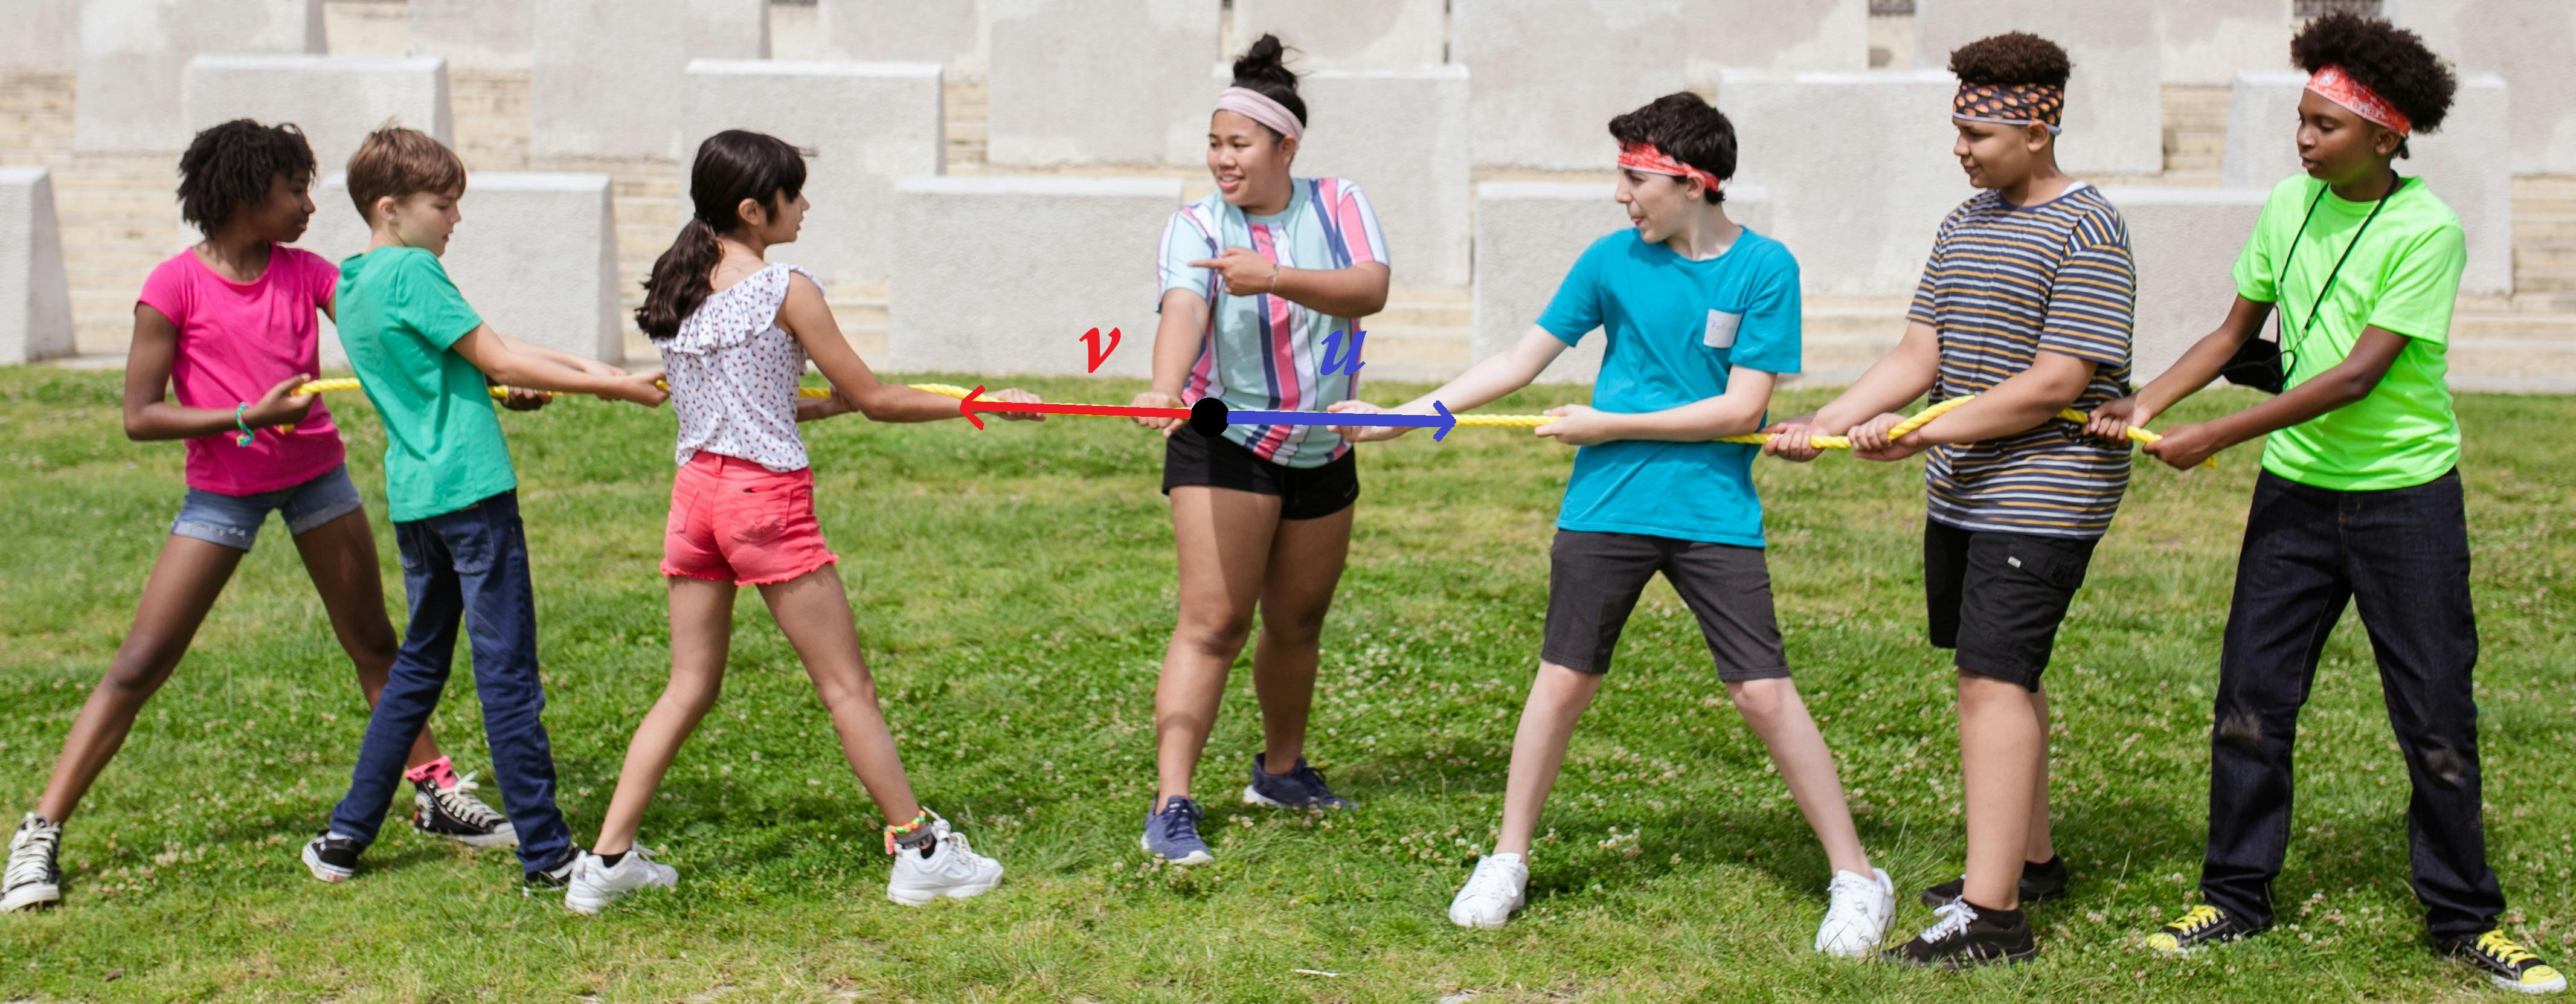
\includegraphics[width=0.7\textwidth]{chapters/chp1_pics/tugofwar_vec.jpg}
    \caption{\textit{Tug-of-war as a visual analogy for vector addition.}}
    \label{fig:tug_of_war}
\end{figure}

\noindent We may also consider by itself, a negative vector \(-\mathbf{v} \) with the same magnitude but an opposite direction. For a vector \( \mathbf{v} \), the negative vector \( -\mathbf{v} \) reverses all components:
\[
-\mathbf{v} = \langle -v_x, -v_y, -v_z \rangle.
\]
\noindent Negative vectors are useful in subtraction, as subtracting a vector is the same as adding its negative: \( \mathbf{u} - \mathbf{v} = \mathbf{u} + (-\mathbf{v}) \).

\subsubsection*{Scalar Multiplication}

\noindent Scalar multiplication scales a vector by a constant factor. If \( c \) is a scalar and \( \mathbf{v} = \langle v_x, v_y, v_z \rangle \), then:
\[
c\mathbf{v} = \langle c v_x, c v_y, c v_z \rangle.
\]

\noindent This means that each component of \( \mathbf{v} \) is multiplied by \( c \), effectively stretching or shrinking the vector by a factor of \( c \). If \( c > 1 \), the vector’s magnitude increases; if \( 0 < c < 1 \), it decreases. \\ \\ For example, doubling the force in a tug-of-war scenario would double each component of the vector representing that force, effectively making the pull twice as strong but in the same direction. Together, vector addition and scalar multiplication allow us to construct complex combinations of vectors and to adjust their magnitudes while maintaining direction, providing a powerful foundation for vector operations in physics and engineering. We may visualize the negative vector and scalar multiplication on the graph below:

\begin{figure}[H]
    \centering
    \begin{tikzpicture}
        % Axes
        \draw[thick,->] (-4,0) -- (5,0) node[right] {$x$};
        \draw[thick,->] (0,-3) -- (0,5) node[above] {$y$};

        % Original vector v with manual label positioning
        \draw[ultra thick,->,blue] (0,0) -- (3,2);
        \node[anchor=north west] at (1.6,1.2) {$\mathbf{v}$};

        % Negative vector -v with manual label positioning
        \draw[ultra thick,->,red] (0,0) -- (-3,-2);
        \node[anchor=north east] at (-1.5,-0.5) {$-\mathbf{v}$};

        % Scaled vector (1/2)v with manual label positioning
        \draw[ultra thick,->,green] (0,0) -- (1.5,1);
        \node[anchor=south west] at (1,0.05) {$\frac{1}{2}\mathbf{v}$};

        % Scaled vector 1.5v with manual label positioning
        \draw[ultra thick,->,purple] (0,0) -- (4.5,3);
        \node[anchor=south east] at (3,2.5) {$1.5\mathbf{v}$};
    \end{tikzpicture}
    \caption{\textit{A vector \( \mathbf{v} \) and its negative counterpart \( -\mathbf{v} \), along with scalar multiples of \( \mathbf{v} \) for various constants.}}
    \label{fig:vector_scalar_multiplication}
\end{figure}

\exampleline
\begin{example}
An engineer is designing a crane to lift materials by applying forces from multiple cables to achieve the required lift and stability. At a particular moment, two cables exert forces represented by the vectors \( \mathbf{F_1} = \langle 120, 0, 80 \rangle \) and \( \mathbf{F_2} = \langle -50, 75, 60 \rangle \), measured in newtons. To achieve a stable lift, determine the combined force applied by both cables, calculate the unit vector in the direction of the combined force, and find a third vector \( \mathbf{G} \) that would need to be added to triple the resultant force from the two cables. Additionally, if we need to fully stabilize the system, calculate the force vector for a third cable \( \mathbf{F_3} \) that would completely counterbalance the combined force.

\begin{solution}
To solve this problem, we’ll use vector addition, scalar multiplication, unit vector concepts, and explore how to achieve both triple force and full stability.

\begin{enumerate}
    \item Combine the Forces by Vector Addition: The combined force vector \( \mathbf{F} = \mathbf{F_1} + \mathbf{F_2} \) is found by adding the components of \( \mathbf{F_1} \) and \( \mathbf{F_2} \):
    \[
    \mathbf{F} = \langle 120 + (-50), 0 + 75, 80 + 60 \rangle = \langle 70, 75, 140 \rangle
    \]

    \item Calculate the Magnitude of the Combined Force: The magnitude \( |\mathbf{F}| \) of the combined force vector \( \mathbf{F} \) is given by:
    \[
    |\mathbf{F}| = \sqrt{70^2 + 75^2 + 140^2} = \sqrt{4900 + 5625 + 19600} = \sqrt{30125} \approx 173.6 \text{ newtons}
    \]

    \item Find the Unit Vector in the Direction of the Combined Force: The unit vector \( \mathbf{u} \) in the direction of \( \mathbf{F} \) is calculated by dividing each component by \( |\mathbf{F}| \):
    \[
    \mathbf{u} = \frac{\mathbf{F}}{|\mathbf{F}|} = \left\langle \frac{70}{173.6}, \frac{75}{173.6}, \frac{140}{173.6} \right\rangle \approx \langle 0.403, 0.432, 0.806 \rangle
    \]

    \item Determine the Vector \( \mathbf{G} \) to Triple the Combined Force: To triple the resultant force, we need a new vector \( \mathbf{G} \) such that the total force becomes \( 3\mathbf{F} \). This means:
    \[
    \mathbf{G} = 3\mathbf{F} - \mathbf{F} = 2\mathbf{F} = 2 \times \langle 70, 75, 140 \rangle = \langle 140, 150, 280 \rangle
    \]
    Therefore, the vector \( \mathbf{G} \) that would need to be applied to triple the combined force is:
    \[
    \mathbf{G} = \langle 140, 150, 280 \rangle
    \]

    \item Determine the Counterbalancing Force Vector \( \mathbf{F_3} \): To fully stabilize the system, we need a third cable with force vector \( \mathbf{F_3} \) that exactly counterbalances the combined force \( \mathbf{F} \). This means \( \mathbf{F_3} \) must be equal in magnitude but opposite in direction to \( \mathbf{F} \), so:
    \[
    \mathbf{F_3} = -\mathbf{F} = \langle -70, -75, -140 \rangle
    \]
    Applying this force would bring the net force to zero, stabilizing the system entirely.

\end{enumerate}

\noindent Thus, the combined force vector of the two cables is \( \langle 70, 75, 140 \rangle \) newtons, with a unit direction vector \( \langle 0.403, 0.432, 0.806 \rangle \). To triple this force, a third vector \( \mathbf{G} = \langle 140, 150, 280 \rangle \) would be added. Finally, a fourth force vector, cable three, \( \mathbf{F_3} = \langle -70, -75, -140 \rangle \) would stabilize the system by perfectly counterbalancing the combined force.

\end{solution}
\end{example}
\exampleline


\vspace{1.3em}


\noindent We've covered addition and subtraction of vectors, which have intuitive meanings in terms of combining directions and magnitudes. However, multiplication raises an important question: how do we interpret multiplying vectors? Here, the dot and cross products offer two distinct perspectives. The dot product provides a scalar, measuring alignment between vectors, while the cross product results in a new vector, perpendicular to both. Simply multiplying components wouldn’t capture these meaningful outcomes, so dot and cross products arise naturally as solutions to vector multiplication.


\subsection*{Dot Product} \index{Dot Product}

The \textit{dot product} (or scalar product) of two vectors \( \mathbf{u} = \langle u_x, u_y, u_z \rangle \) and \( \mathbf{v} = \langle v_x, v_y, v_z \rangle \) measures how much one vector “projects” onto another. This projection quantifies how much of one vector’s length is aligned in the direction of the other. Mathematically, the dot product is defined as:
\[
\mathbf{u} \cdot \mathbf{v} = u_x v_x + u_y v_y + u_z v_z.
\]
While this formula looks straightforward, it can be re-expressed to reveal a deeper interpretation by relating it to the angle \( \theta \) between \( \mathbf{u} \) and \( \mathbf{v} \):
\[
\mathbf{u} \cdot \mathbf{v} = |\mathbf{u}| |\mathbf{v}| \cos \theta.
\]
This alternate form shows that the dot product depends on the magnitudes of \( \mathbf{u} \) and \( \mathbf{v} \) and their alignment. To understand where \( \cos \theta \) comes into play, recall that we previously introduced direction cosines to describe a vector’s orientation. In the dot product, \( \cos \theta \) arises because the product measures how well-aligned two vectors are. When two vectors point in the same direction, \( \theta = 0 \) (cosine of 0° is 1), and the dot product is simply \( |\mathbf{u}| |\mathbf{v}| \). If the vectors are perpendicular (at 90°, or \( \pi/2 \) radians), \( \cos \theta = 0 \), and the dot product is zero, meaning there’s no overlap in direction.

\begin{figure}[H]
    \centering
    \begin{tikzpicture}
        % Axes
        \draw[thick,->] (-1,0) -- (5,0) node[right] {$x$};
        \draw[thick,->] (0,-1) -- (0,3) node[above] {$y$};
        
        % Vectors u and v
        \draw[ultra thick,->,blue] (0,0) -- (3,1) node[anchor=south west] at (1.6,0.6) {$\mathbf{u}$};
        \draw[ultra thick,->,red] (0,0) -- (2,3) node[anchor=south east] at (1.4,2) {$\mathbf{v}$};
        
        % Projection line from v onto u
        \draw[dashed] (2,3) -- (3,1);
        
        % Angle theta
        \draw[thick,->] (1,.36) arc[start angle=0,end angle=43,radius=1] node[midway, right] {$\theta$};
        
        % Label for |v| cos theta projection
        \node[anchor=north west] at (3.1,1.6) {$|\mathbf{v}| \cos \theta$};
    \end{tikzpicture}
    \caption{\textit{The dot product as the projection of \( \mathbf{v} \) onto \( \mathbf{u} \), scaled by \( \cos \theta \).}}
    \label{fig:dot_product_projection}
\end{figure}

\noindent \textbf{Real-World Example: Work Done by a Force.} A common example of the dot product is the calculation of work done by a force acting over a displacement. If a force \( \mathbf{F} \) is applied to move an object by a displacement \( \mathbf{d} \), then the work done \( W \) is:
\[
W = \mathbf{F} \cdot \mathbf{d} = |\mathbf{F}| |\mathbf{d}| \cos \theta.
\]
In this expression, only the component of the force that aligns with the displacement contributes to work. To make this intuitive, think about closing a door: if you push on the door in a direction perfectly perpendicular to its plane (where \( \theta = 90^\circ \) or \( \pi/2 \)), the force is wasted because \( \cos(90^\circ) = 0 \), and no work is done to close the door. However, when you push directly along the direction of the door’s swing (at \( \theta = 0^\circ \)), the cosine is maximized, allowing the full force to contribute to moving the door. \\ \\ Thus, the dot product is valuable because it captures not just magnitude but the idea of alignment, making it essential in scenarios where only the aligned portion of a force (or vector) is relevant to an outcome.

\exampleline
\begin{example}
Given vectors \( \mathbf{a} = \langle 3, 0, 4 \rangle \) and \( \mathbf{b} = \langle 1, 2, -1 \rangle \), calculate their dot product and interpret the result.

\begin{solution}
The dot product \( \mathbf{a} \cdot \mathbf{b} \) is computed as:
\[
\mathbf{a} \cdot \mathbf{b} = (3)(1) + (0)(2) + (4)(-1).
\]

Calculating each term:
\begin{align*}
    3 \cdot 1 &= 3, \\
    0 \cdot 2 &= 0, \\
    4 \cdot (-1) &= -4.
\end{align*}

Adding these results, we get:
\[
\mathbf{a} \cdot \mathbf{b} = 3 + 0 - 4 = -1.
\]

The dot product \( -1 \) indicates that \( \mathbf{a} \) and \( \mathbf{b} \) are not aligned, as a positive result would imply some degree of alignment in the same direction. The negative value suggests that \( \mathbf{a} \) and \( \mathbf{b} \) point in somewhat opposite directions along their components.

\end{solution}
\end{example}
\exampleline


\subsection*{Cross Product} \index{Cross Product}

The \textit{cross product} (or vector product) of two vectors \( \mathbf{u} = \langle u_x, u_y, u_z \rangle \) and \( \mathbf{v} = \langle v_x, v_y, v_z \rangle \) gives a new vector that is perpendicular, or \textit{normal} to both \( \mathbf{u} \) and \( \mathbf{v} \). The cross product is defined such that the resulting vector points in a direction determined by the \textit{right-hand rule}: if you point your right hand’s index finger along \( \mathbf{u} \) and your middle finger along \( \mathbf{v} \), then your thumb points in the direction of \( \mathbf{u} \times \mathbf{v} \). The magnitude of this vector corresponds to the area of the parallelogram spanned by \( \mathbf{u} \) and \( \mathbf{v} \), given by:
\[
\mathbf{n} = \mathbf{u} \times \mathbf{v} = \langle u_y v_z - u_z v_y, u_z v_x - u_x v_z, u_x v_y - u_y v_x \rangle.
\]

\noindent An alternative way to calculate the cross product is by using the \textit{determinant} of a \( 3 \times 3 \) matrix (maybe you have heard of this in linear algebra before). In this method, we set up a matrix with the unit vectors \( \mathbf{i} \), \( \mathbf{j} \), and \( \mathbf{k} \) in the first row, the components of \( \mathbf{u} \) in the second row, and the components of \( \mathbf{v} \) in the third row:
\[
\mathbf{u} \times \mathbf{v} = \begin{vmatrix} \mathbf{i} & \mathbf{j} & \mathbf{k} \\ u_x & u_y & u_z \\ v_x & v_y & v_z \end{vmatrix}.
\]

To compute this determinant, we expand along the first row:
\[
\mathbf{u} \times \mathbf{v} = \mathbf{i} \begin{vmatrix} u_y & u_z \\ v_y & v_z \end{vmatrix} - \mathbf{j} \begin{vmatrix} u_x & u_z \\ v_x & v_z \end{vmatrix} + \mathbf{k} \begin{vmatrix} u_x & u_y \\ v_x & v_y \end{vmatrix}.
\]

Each \( 2 \times 2 \) determinant is calculated as follows:
\[
\begin{vmatrix} a & b \\ c & d \end{vmatrix} = a d - b c.
\]

Applying this to our cross product:
\[
\mathbf{u} \times \mathbf{v} = \mathbf{i} (u_y v_z - u_z v_y) - \mathbf{j} (u_x v_z - u_z v_x) + \mathbf{k} (u_x v_y - u_y v_x).
\]

Thus, we arrive at the same result as before:
\[
\mathbf{u} \times \mathbf{v} = \langle u_y v_z - u_z v_y, u_z v_x - u_x v_z, u_x v_y - u_y v_x \rangle.
\]

\noindent Using the determinant method provides a structured way to calculate the cross product and reinforces the concept of orientation in three-dimensional space. \\ \\ The magnitude of the cross product is given by:
\[
|\mathbf{u} \times \mathbf{v}| = |\mathbf{u}| |\mathbf{v}| \sin \theta,
\]
where \( \theta \) is the angle between \( \mathbf{u} \) and \( \mathbf{v} \). This value is maximized when \( \mathbf{u} \) and \( \mathbf{v} \) are perpendicular (where \( \sin \theta = 1 \)) and zero when the vectors are parallel, indicating no area spanned.

\noindent The magnitude of the cross product is significant because it represents the area of the parallelogram formed by \( \mathbf{u} \) and \( \mathbf{v} \). \\ \\ Geometrically, this area provides a measure of how ``spread out" the two vectors are relative to each other. If the vectors are aligned (parallel), there’s no area between them, so the magnitude is zero. When the vectors are perpendicular, they span the maximum possible area, with the magnitude equal to \( |\mathbf{u}| |\mathbf{v}| \). This concept is especially useful in physics and engineering, where the cross product’s magnitude can indicate quantities like torque or rotational force, which depend on both the strength and the orientation of the applied forces. We observe a visualization below:

\begin{figure}[H]
    \centering
\begin{tikzpicture}[scale=2]
\draw[-,fill=white!95!red](0,0)--(3,0)--(4,1)--(1,1)--cycle;
\node at (2,0.5) {$|\textcolor{blue}{\mathbf{a}}\times \textcolor{red}{\mathbf{b}}|$};
\draw[ultra thick,-latex,blue](0,0)--(3,0)node[midway,below]{$\mathbf{a}$};
\draw[ultra thick,-latex,red](0,0)--(1,1)node[midway,above]{$\mathbf{b}$};
\draw[ultra thick,-latex,blue!50!red](0,0)--(0,2.1)node[pos=0.7,right]{$\mathbf{n} = \mathbf{a}\times \mathbf{b}$};
\draw (0.6,0) arc [start angle=0,end angle=45,radius=0.6]
node[pos=0.7,right]{$\theta$};
\end{tikzpicture}
    \caption{\textit{Visualization of the cross product \( \mathbf{a} \times \mathbf{b} \), showing the area spanned by vectors \( \mathbf{a} \) and \( \mathbf{b} \), as well as the normal vector direction $\mathbf{n}$.}}
    \label{fig:cross_product_area}
\end{figure}

\exampleline
\begin{example}
Compute the following cross products:
\begin{enumerate}
   \item $\langle 1, 5, 7\rangle \times \langle -4, 3, 3.2\rangle$
   \item $\langle xy^2, z^2, x\rangle \times \langle y, x, z\rangle$
\end{enumerate}

\begin{solution}
\begin{enumerate}
   \item Using the determinant method:
   \[
   \begin{vmatrix}
   \mathbf{i} & \mathbf{j} & \mathbf{k} \\
   1 & 5 & 7 \\
   -4 & 3 & 3.2
   \end{vmatrix}
   \]
   \[
   \begin{aligned}
   i &= \begin{vmatrix} 5 & 7 \\ 3 & 3.2 \end{vmatrix} 
       = 5 \cdot 3.2 \;-\; 7 \cdot 3 
       = 16 - 21 
       = -5 \\[1ex]
   j &= -\begin{vmatrix} 1 & 7 \\ -4 & 3.2 \end{vmatrix} 
       = -\bigl(1 \cdot 3.2 - 7 \cdot (-4)\bigr) 
       = -\bigl(3.2 + 28\bigr) 
       = -31.2 \\[1ex]
   k &= \begin{vmatrix} 1 & 5 \\ -4 & 3 \end{vmatrix} 
       = 1 \cdot 3 \;-\; 5 \cdot (-4) 
       = 3 + 20 
       = 23
   \end{aligned}
   \]
   \[
   \langle 1, 5, 7\rangle \times \langle -4, 3, 3.2\rangle 
   = \langle -5, -31.2, 23\rangle
   \]

   \item Using the same method:
   \[
   \begin{vmatrix}
   \mathbf{i} & \mathbf{j} & \mathbf{k} \\
   xy^2 & z^2 & x \\
   y & x & z
   \end{vmatrix}
   \]
   \[
   \begin{aligned}
   i &= \begin{vmatrix} z^2 & x \\ x & z \end{vmatrix}
       = z^2 \cdot z \;-\; x \cdot x
       = z^3 - x^2 \\[1ex]
   j &= -\begin{vmatrix} xy^2 & x \\ y & z \end{vmatrix}
       = -\bigl(xy^2 \cdot z \;-\; x \cdot y\bigr)
       = -(xy^2z - xy)
       = xy(1 - yz) \\[1ex]
   k &= \begin{vmatrix} xy^2 & z^2 \\ y & x \end{vmatrix}
       = xy^2 \cdot x \;-\; z^2 \cdot y
       = x^2y^2 - yz^2
   \end{aligned}
   \]
   \[
   \langle xy^2, z^2, x\rangle \times \langle y, x, z\rangle 
   = \langle z^3 - x^2, \; xy(1-yz), \; x^2y^2 - yz^2 \rangle
   \]
\end{enumerate}
\end{solution}
\end{example}
\exampleline



\subsubsection*{The Right-Hand Rule}
\noindent The right-hand rule provides an intuitive way to determine the orientation of the cross product vector. As you point your right hand’s index finger along the direction of \( \mathbf{u} \) and your middle finger along \( \mathbf{v} \), your thumb will naturally point in the direction of \( \mathbf{u} \times \mathbf{v} \). This orientation represents a unique perpendicular direction relative to both vectors. \\ \\  \textbf{Uniqueness and Ambiguity of the Normal Vector.} The normal vector \( \mathbf{u} \times \mathbf{v} \) is unique in that it provides a consistent perpendicular direction, yet there is also an inherent ambiguity: for any two vectors, two possible perpendicular directions exist. The right-hand rule helps us choose one of these consistently, giving us a convention for which perpendicular direction to use. However, if we were to reverse the order, calculating \( \mathbf{v} \times \mathbf{u} \) instead, the resulting vector would point in the opposite direction. \\ \\ \textbf{Real-World Example: Torque.} In engineering, the cross product is essential in calculating torque, the rotational effect of a force around an axis. If a force \( \mathbf{F} \) is applied at a point represented by the position vector \( \mathbf{r} \), the torque \( \boldsymbol{\tau} \) around the pivot point is:
\[
\boldsymbol{\tau} = \mathbf{r} \times \mathbf{F}.
\]
Here, the torque vector \( \boldsymbol{\tau} \) is perpendicular to the plane formed by \( \mathbf{r} \) and \( \mathbf{F} \), and its magnitude gives the rotational effect or leverage created by \( \mathbf{F} \). This example shows how cross products are useful when interactions involve rotation or orientation. \\ \\ \textbf{Geometric Interpretation of Cross Product:} The cross product also provides a way to measure the area spanned by two vectors. When we construct a parallelogram with \( \mathbf{u} \) and \( \mathbf{v} \) as adjacent sides, the magnitude of \( \mathbf{u} \times \mathbf{v} \) represents the area of this parallelogram. This interpretation is valuable in physics and engineering applications where the area or spatial orientation between vectors is critical.

\begin{figure}[H]
    \centering
    \begin{tikzpicture}[
        vec/.style={thick,[-)},
    ]
        % Coordinates for vector placement
        \coordinate (A) at (3,0);
        \coordinate (B) at (0,-2);
        \coordinate (cross prod) at (1,4);
        \def\tick{0.2}
        
        % Axes
        \draw [->] (-1,0) -- (6,0) node [below] {$x$};
        \draw [->] (0,-1) -- (0,5) node [left]  {$y$};
        
        % Grid ticks
        \foreach \x in {1,...,5}
            \draw (\x,\tick/2) -- ++(0,-\tick) node [below] {\x};
        \foreach \y in {1,...,4}
            \draw (\tick/2,\y) -- ++(-\tick,0) node [left] {\y};
        
        % Vectors A and B
        \draw [vec,->,blue] (1,-1) -- ++(A) node [midway,below] {$\mathbf{u}$};
        \draw [vec,->,red] (-1,4) -- ++(B) node [midway,left]  {$\mathbf{v}$};
        
        % Box representing the parallelogram area
        \fill [gray, opacity=0.3] (cross prod) rectangle ++($(A)+(B)$);
        \draw [thick] ($(cross prod)+(A)$) -| ($(cross prod)+(B)$);
        \draw [thick,dashed] ($(cross prod)+(A)$) |- ($(cross prod)+(B)$)
            node [pos=0.25,right] {$\mathbf{u} \times \mathbf{v}$};
    \end{tikzpicture}
    \caption{\textit{Completing the parallelogram using the cross product \( \mathbf{u} \times \mathbf{v} \), representing the area spanned by vectors \( \mathbf{u} \) and \( \mathbf{v} \).}}
    \label{fig:cross_product_parallelogram}
\end{figure}


\subsection*{Parallelepipeds}

\noindent A \textit{parallelepiped} is a three-dimensional figure formed by six parallelograms. It is defined by three vectors \( \mathbf{u}, \mathbf{v}, \) and \( \mathbf{w} \) that emanate from the same point. The volume of a parallelepiped provides a geometric interpretation of the scalar triple product, which combines the concepts of dot and cross products. \\ \\ The volume \( V \) of a parallelepiped defined by \( \mathbf{u}, \mathbf{v}, \mathbf{w} \) is given by:
\[
V = |\mathbf{u} \cdot (\mathbf{v} \times \mathbf{w})|.
\]

\noindent \textbf{Why this formula works:}
\begin{itemize}
    \item The cross product \( \mathbf{v} \times \mathbf{w} \) gives a vector perpendicular to the parallelogram formed by \( \mathbf{v} \) and \( \mathbf{w} \), with a magnitude equal to the area of this parallelogram.
    \item Taking the dot product \( \mathbf{u} \cdot (\mathbf{v} \times \mathbf{w}) \) projects \( \mathbf{u} \) onto the direction of \( \mathbf{v} \times \mathbf{w} \), yielding the ``height" of the parallelepiped.
    \item Multiplying the height by the base area (given by the cross product) gives the volume.
\end{itemize}

Below is a plot of a parallelepiped:




\begin{figure}[H]
    \centering
\tdplotsetmaincoords{70}{60}
   \begin{tikzpicture}[
line cap=butt, line join=round,
tdplot_main_coords,
declare function={a=3;b=4;h=3;k=2;}
   ]
    \begin{scope}[canvas is xy plane at z=0]
    \path
    (0,0) coordinate    (A)
    (a,0) coordinate    (B)
    (a,b) coordinate    (C)
    (0,b) coordinate    (D);
    \end{scope}
    \begin{scope}[canvas is xy plane at z=h]
    \path
    (0,k) coordinate    (A')
    (a,k) coordinate    (B')
    (a,b+k) coordinate  (C')
    (0,b+k) coordinate  (D');
    \end{scope}
    \begin{scope}[opacity=0.3, thick]
    \draw[fill=orange] (A) -- (B) -- (C) -- (D) -- cycle;
    \draw[fill=orange] (A) -- (B) -- (B') -- (A') -- cycle;
    \draw[fill=orange] (B) -- (C) -- (C') -- (B') -- cycle;
    \draw[fill=orange] (C) -- (D) -- (D') -- (C') -- cycle;
    \draw[fill=orange] (A) -- (D) -- (D') -- (A') -- cycle;
    \draw[fill=orange] (A') -- (B') -- (C') -- (D') -- cycle;
    \end{scope}

    % Original vectors in the parallelepiped
    \draw[thick, -{Straight Barb[scale=0.8]}] (A) -- (B);
    \draw[thick, -{Straight Barb[scale=0.8]}] (A) -- (D);
    \draw[thick, -{Straight Barb[scale=0.8]}] (A) -- (A');

    % Labels for vectors u, v, w with adjustable positions
    \node at (1.5, -0.5, 0) {\( \mathbf{u} \)}; % Adjust position for \( u \)
    \node at (0.5, 2.5, 0) {\( \mathbf{v} \)}; % Adjust position for \( v \)
    \node at (0.5, 0.5, 2) {\( \mathbf{w} \)}; % Adjust position for \( w \)}
    
    \end{tikzpicture}
    \caption{\textit{A parallelepiped spanned by vectors \( \mathbf{u}, \mathbf{v}, \mathbf{w} \) originating at the origin.}}
    \label{fig:parallelepiped}
\end{figure}



\exampleline
\begin{example}
Given vectors \( \mathbf{a} = \langle 3, 0, 4 \rangle \) and \( \mathbf{b} = \langle 1, 2, -1 \rangle \), calculate their cross product.

\begin{solution}
The cross product \( \mathbf{a} \times \mathbf{b} \) is computed as:
\[
\mathbf{a} \times \mathbf{b} = \langle 0 \cdot (-1) - 4 \cdot 2, 4 \cdot 1 - 3 \cdot (-1), 3 \cdot 2 - 0 \cdot 1 \rangle.
\]

Calculating each component:
\begin{align*}
    x\text{-component} &= 0 \cdot (-1) - 4 \cdot 2 = -8, \\
    y\text{-component} &= 4 \cdot 1 - 3 \cdot (-1) = 4 + 3 = 7, \\
    z\text{-component} &= 3 \cdot 2 - 0 \cdot 1 = 6.
\end{align*}

Thus, \( \mathbf{a} \times \mathbf{b} = \langle -8, 7, 6 \rangle \).
\end{solution}
\end{example}
\exampleline





\subsection*{Applications of Vectors in Three Dimensions and Higher}

\noindent Vectors are essential tools across various fields due to their ability to represent both magnitude and direction. Some of the most common applications include:

\begin{itemize}
    \item In \textbf{physics}, vectors describe physical quantities like forces, velocities, and accelerations in three-dimensional space, which helps analyze motion and interactions. For instance, Newton’s Second Law of Motion can be written with vectors as:
    \[
    \mathbf{F} = m \mathbf{a},
    \]
    where \( \mathbf{F} \) is the force vector, \( m \) is the mass, and \( \mathbf{a} \) is the acceleration vector. Vectors also appear in equations for gravitational force. For two masses \( m_1 \) and \( m_2 \) separated by a distance vector \( \mathbf{r} \), the gravitational force is:
    \[
    \mathbf{F}_{\text{gravity}} = -G \frac{m_1 m_2}{|\mathbf{r}|^2} \hat{\mathbf{r}},
    \]
    where \( G \) is the gravitational constant, and \( \hat{\mathbf{r}} \) is the unit vector in the direction of \( \mathbf{r} \). These vector equations help us break down forces into components, making it easier to understand the effects in each direction.

    \item In \textbf{engineering}, vectors represent stresses, displacements, and rotations within structures, which aids in designing stable structures. For example, vectors help engineers analyze how much force a bridge can handle by representing forces and movements in each direction. Stress and strain can also be represented with multi-dimensional vectors or matrices, providing insights into material behavior under different loads.

    \item In \textbf{computer graphics}, vectors are crucial for simulating lighting, shading, and movement in three-dimensional environments. For example, when calculating the lighting on a surface, we use the \textit{dot product} between the light direction vector \( \mathbf{L} \) and the surface normal vector \( \mathbf{N} \) to find the light’s intensity on that surface:
    \[
    I = I_{\text{light}} \cdot \max(0, \mathbf{L} \cdot \mathbf{N}),
    \]
    where \( I \) is the resulting intensity, and \( I_{\text{light}} \) is the light source intensity. This helps create realistic shading by adjusting brightness based on the angle between the light and the surface.
\end{itemize}

\noindent Vectors are also powerful for thinking beyond physical three-dimensional space. In fields like machine learning and quantum mechanics, vectors allow us to work in higher-dimensional, abstract spaces:

\begin{itemize}
    \item In \textbf{machine learning}, vectors represent data points with multiple features. For example, if each data point has 100 features, we can think of it as a vector in a 100-dimensional space. By measuring distances between these vectors, we can find similarities between data points. For instance, the Euclidean distance between two data points \( \mathbf{x} \) and \( \mathbf{y} \) is:
    \[
    \text{Distance}(\mathbf{x}, \mathbf{y}) = \sqrt{\sum_{i=1}^n (x_i - y_i)^2},
    \]
    where \( \mathbf{x} \) and \( \mathbf{y} \) are vectors representing two data points. The dot product is also used in machine learning algorithms like support vector machines to classify data by finding directions that separate categories. Neural networks rely heavily on matrix-vector multiplication, which is an extension of vector operations, to process and transform data through layers.

    \item In \textbf{quantum mechanics}, vectors represent quantum states in complex, high-dimensional spaces. For instance, a basic quantum unit, a qubit, can be represented by a vector in a two-dimensional complex space:
    \[
    |\psi\rangle = \alpha |0\rangle + \beta |1\rangle,
    \]
    where \( \alpha \) and \( \beta \) are complex numbers satisfying \( |\alpha|^2 + |\beta|^2 = 1 \). The dot product (or inner product) between two quantum state vectors gives probabilities for measurement outcomes, which is central to quantum calculations.
\end{itemize}

\noindent These examples show that vectors are more than just arrows in space. They allow us to work with quantities that have both size and direction, whether we're studying forces in physics or organizing data in machine learning. By using vectors, we can extend our understanding into higher-dimensional spaces, making them indispensable tools in both theoretical and applied fields.


\exampleline
\begin{example}
Suppose we have two products represented by feature vectors:
\[
\mathbf{p} = \langle 8, 2, 15 \rangle \quad \text{and} \quad \mathbf{q} = \langle 5, 3, 12 \rangle,
\]
where each vector component represents the popularity, weight (in kg), and price (in dollars) of each product, respectively. In machine learning, we often use vector operations like the dot product and cross product to analyze relationships between data points (in this case, the products). Let’s calculate:
\begin{enumerate}
    \item The dot product \( \mathbf{p} \cdot \mathbf{q} \) to measure the similarity between the products in terms of their features.
    \item The cross product \( \mathbf{p} \times \mathbf{q} \) to analyze how the products differ across the feature space.
\end{enumerate}

\begin{solution}
We’ll go through each calculation step-by-step.

\begin{enumerate}
    \item \textbf{Dot Product:}

    \noindent The dot product is useful for assessing similarity between vectors. When comparing products, a higher dot product value suggests that the products share similar feature characteristics. Here, we calculate the dot product as:
    \[
    \mathbf{p} \cdot \mathbf{q} = (8)(5) + (2)(3) + (15)(12) = 40 + 6 + 180 = 226.
    \]
    In this case, a dot product of 226 implies moderate alignment between the products' popularity, weight, and price. In a recommendation system, for example, a higher dot product might indicate that two products could appeal to similar customers.

    \item \textbf{Cross Product:}

    \noindent The cross product results in a new vector perpendicular to both \( \mathbf{p} \) and \( \mathbf{q} \). In machine learning, this can help identify unique directions in the feature space where the products differ significantly, which can be useful for clustering or classification tasks to understand how data points vary in multiple dimensions. The cross product is calculated as:
    \[
    \mathbf{p} \times \mathbf{q} = \langle 2 \cdot 12 - 15 \cdot 3, 15 \cdot 5 - 8 \cdot 12, 8 \cdot 3 - 2 \cdot 5 \rangle.
    \]

    \noindent Calculating each component:
    \begin{align*}
        x\text{-component} &= (2)(12) - (15)(3) = 24 - 45 = -21, \\
        y\text{-component} &= (15)(5) - (8)(12) = 75 - 96 = -21, \\
        z\text{-component} &= (8)(3) - (2)(5) = 24 - 10 = 14.
    \end{align*}

    \noindent Thus, the cross product \( \mathbf{p} \times \mathbf{q} = \langle -21, -21, 14 \rangle \).
    
    \noindent This cross product vector, \( \langle -21, -21, 14 \rangle \), highlights the directional differences between the products. In some machine learning applications, such as Principal Component Analysis (PCA), understanding these directions helps in finding dimensions that best separate or distinguish data points.

\end{enumerate}

\noindent \textbf{Summary:} In this example:
\begin{itemize}
    \item The dot product of 226 suggests that the products have moderate similarity in their features. This measure could help a recommendation algorithm group these items as similar.
    \item The cross product \( \langle -21, -21, 14 \rangle \) represents the direction of variance between these products, useful for exploring the distinctiveness of feature combinations in high-dimensional analysis.
\end{itemize}
\end{solution}
\end{example}
\exampleline



\vspace{1.3em}

\noindent The following Python programming example demonstrates how dot and cross products can be applied in machine learning to measure similarity and analyze differences between feature vectors of products. Dot products are used here as a basic similarity score, while cross products provide insight into directional differences across features -- much like what we have done in the previous example. Students can run the following Python code to experiment with these concepts in a real-world context:
\index{Python}

\vspace{1.3em}

\begin{lstlisting}
import numpy as np

# Feature vectors for two products: [popularity, weight (kg), price (dollars)]
p = np.array([8, 2, 15])
q = np.array([5, 3, 12])

# Calculate the dot product
dot_product = np.dot(p, q)
print(f"Dot Product (Similarity Score): {dot_product}")

# Calculate the cross product
cross_product = np.cross(p, q)
print(f"Cross Product (Directional Difference): {cross_product}")

# Use dot product as a basic similarity measure for recommendation
similarity_threshold = 200  # Set an arbitrary threshold
if dot_product > similarity_threshold:
    print("Products are similar enough to recommend together.")
else:
    print("Products are distinct enough to consider separately.")

# Analyze uniqueness with cross product
if np.linalg.norm(cross_product) > 0:
    print("Products have unique directional attributes across feature space.")
else:
    print("Products are very similar across all feature dimensions.")
\end{lstlisting}


\newpage









\lecture{Lines and Planes in Space} \index{Lines} \index{Planes}


\noindent As we extend our understanding of vectors and coordinate systems from two dimensions to three, we encounter new challenges and possibilities. In two-dimensional space, we could represent points, lines, and directions relatively simply. But as we move into three dimensions, we need to adapt our definitions to handle the additional complexity of this expanded space. Naturally, we begin asking questions like: \textit{How do we represent a line in 3D? How do we define a flat surface, or plane, that extends in multiple directions in this space?} \\ \\ Using what we know about vectors and coordinate systems, we can build definitions for lines and planes in 3D that feel like natural extensions of the concepts we used in 2D. In 2D, a line could be defined by a point and a direction (often represented by a slope). In 3D, however, a line requires both a point for positioning and a vector to set its direction in this more complex space. Similarly, defining a plane in 3D requires a point and a vector that establishes its orientation. Developing these definitions is key to understanding and navigating three-dimensional space.

\subsection*{Equations of Lines and Line Segments}

\noindent In mathematics, we often represent points and vectors with similar symbols, but it is crucial to distinguish between them as they serve different purposes in geometry. A point, denoted as \( P \), represents a specific location in space, typically described by its coordinates \( (x, y, z) \). For instance, when we write \( P = (x_0, y_0, z_0) \), we are explicitly identifying a unique position in space. \\ \\  On the other hand, when we use bold notation such as \( \mathbf{P} \) (e.g., \( \mathbf{P_0} \) or \( \mathbf{P_1} \)), we are explicitly treating it as a \textbf{position vector}. A position vector originates from the origin and ``points” to the coordinates of \( P \). In this case, \( \mathbf{P} = \langle x, y, z \rangle \) represents a vector that extends from the origin to the location \( (x, y, z) \).  When a point \( (x, y, z) \) is to be used in vector calculations, it is written as \( \mathbf{P} \). This explicit use of bold notation highlights that the point is being treated as a vector, enabling operations such as addition, subtraction, and scaling to describe directions, magnitudes, and displacements in space. \\ \\ To summarize:
\begin{itemize}
    \item \( P \) refers to a specific point at coordinates \( (x, y, z) \), which identifies a location.
    \item \( \mathbf{P} = \langle x, y, z \rangle \) explicitly represents the position vector pointing from the origin to \( P \).
    \item When a point is to be used as a vector in calculations, we write it as \( \mathbf{P} \) to make its vectorial role explicit.
\end{itemize}

\noindent In this context, \( \mathbf{P} \) will always be used when working with vectors in calculations, ensuring clarity and consistency, while \( P \) is reserved to identify specific points independent of vectors. By maintaining this distinction, we make the roles of points and vectors explicit in both notation and interpretation.


\subsubsection*{Defining a Line in 3D Space}

\noindent To describe a line in three-dimensional space, we need:
\begin{itemize}
    \item A specific \textbf{point} through which the line passes, denoted \( \mathbf{P_0} = (x_0, y_0, z_0) \).
    \item A \textbf{direction vector} that defines the orientation of the line, represented by \( \mathbf{d} = \langle a, b, c \rangle \).
\end{itemize}

\noindent The point \( \mathbf{P_0} \) anchors the line at a specific position, while \( \mathbf{d} \) describes how the line extends in space. By combining these, we can reach any point along the line.

\subsubsection*{The Parametric Equation of a Line}

\noindent To generate all points on a line that passes through \( \mathbf{P_0} \) with direction vector \( \mathbf{d} \), we introduce a \textbf{parameter} \( t \) that scales \( \mathbf{d} \). The parametric equation of the line becomes:
\[
\mathbf{r}(t) = \mathbf{P_0} + t \mathbf{d} = \langle x_0 + at, y_0 + bt, z_0 + ct \rangle,
\]
where \( \mathbf{r}(t) \) represents the position vector of any point on the line.

\noindent Breaking down this equation:
\begin{itemize}
    \item When \( t = 0 \), \( \mathbf{r}(0) = \mathbf{P_0} \), locating us at the point \( \mathbf{P_0} \).
    \item As \( t \) varies, we move along the line in the direction of \( \mathbf{d} \).
\end{itemize}

\noindent Alternatively, we can express the parametric form as a set of equations:
\[
\left\{
\begin{aligned}
    x &= x_0 + at, \\
    y &= y_0 + bt, \\
    z &= z_0 + ct,
\end{aligned}
\right.
\quad t \in I,
\]
where \( I \) is the interval for \( t \) that defines the line or line segment.

\subsubsection*{Line Segments}

\noindent If we want only a segment of the line connecting two points \( \mathbf{P_1} = (x_1, y_1, z_1) \) and \( \mathbf{P_2} = (x_2, y_2, z_2) \), we define the line segment using \( t \) in the range \( [0, 1] \). \\ \\ For \( t \in [0, 1] \), the position vector \( \mathbf{r}(t) \) of any point on the line segment is:
\[
\mathbf{r}(t) = (1 - t) \mathbf{P_1} + t \mathbf{P_2} = (1 - t) \langle x_1, y_1, z_1 \rangle + t \langle x_2, y_2, z_2 \rangle.
\]
Expanding this:
\[
\mathbf{r}(t) = \langle (1 - t)x_1 + t x_2, (1 - t)y_1 + t y_2, (1 - t)z_1 + t z_2 \rangle.
\]
This form describes points on the segment:
\begin{itemize}
    \item When \( t = 0 \), \( \mathbf{r}(0) = \mathbf{P_1} = \langle x_1, y_1, z_1 \rangle \).
    \item When \( t = 1 \), \( \mathbf{r}(1) = \mathbf{P_2} = \langle x_2, y_2, z_2 \rangle \).
    \item For \( t \in (0, 1) \), \( \mathbf{r}(t) \) lies between \( \mathbf{P_1} \) and \( \mathbf{P_2} \), tracing the line segment.
\end{itemize}

\noindent This approach uses vector notation to generalize points along the line segment, treating each location as a vector in 3D space.


\begin{figure}[H]
\tdplotsetmaincoords{70}{110}
    \centering
    % Set up the main coordinates for a 3D perspective
    \begin{tikzpicture}[scale=5, tdplot_main_coords]

    % Define points P1 and P2 and the parameter t
    \pgfmathsetmacro{\xone}{0.2}
    \pgfmathsetmacro{\yone}{0.3}
    \pgfmathsetmacro{\zone}{0.4}
    \pgfmathsetmacro{\xtwo}{0.8}
    \pgfmathsetmacro{\ytwo}{0.9}
    \pgfmathsetmacro{\ztwo}{0.6}

    % Draw axes
    \draw[->, thick] (0,0,0) -- (1.2,0,0) node[anchor=west] {$x$};
    \draw[->, thick] (0,0,0) -- (0,1.2,0) node[anchor=west] {$y$};
    \draw[->, thick] (0,0,0) -- (0,0,1.2) node[anchor=south] {$z$};

    % Draw points P1 and P2
    \filldraw[blue] (\xone, \yone, \zone) circle (0.5pt);
    \filldraw[blue] (\xtwo, \ytwo, \ztwo) circle (0.5pt);

    % Draw the line segment between P1 and P2
    \draw[->, blue!70!black, ultra thick] (\xone, \yone, \zone) -- (\xtwo, \ytwo, \ztwo);

    % Labels for P1, P2, and r(t) with manual positioning
    \node[anchor=north east] at (\xone - 0.05, \yone - 0.05, \zone) {$\mathbf{P_1} = (x_1, y_1, z_1)$};
    \node[anchor=south west] at (\xtwo + 0.05, \ytwo + 0.05, \ztwo) {$\mathbf{P_2} = (x_2, y_2, z_2)$};
    \node[anchor=south] at ({(\xone + \xtwo)/2 + 0.1}, {(\yone + \ytwo)/2 + 0.1}, {(\zone + \ztwo)/2 + 0.07}) {$\mathbf{r}(t)$};

    \end{tikzpicture}

    \caption{\textit{The line segment connecting points \( \mathbf{P_1} \) and \( \mathbf{P_2} \) in three-dimensional space, represented by \( \mathbf{r}(t) = (1 - t) \mathbf{P_1} + t \mathbf{P_2} \) for \( 0 \leq t \leq 1 \). Here, \( \mathbf{P_1} \) and \( \mathbf{P_2} \) represent the positions of the endpoints, while \( \mathbf{P_1} \) and \( \mathbf{P_2} \) denote their position vectors.}}
    \label{fig:line_segment}
\end{figure}




\noindent \textbf{Why Use a Line Segment?} Line segments are useful for representing finite parts of lines, such as beams in a structure or paths between points. In many applications, we don’t need the entire line, just a specific portion. In summary, by combining a point with a direction vector, we can describe a line in 3D space. The parametric form gives us flexibility in describing all points on the line and any specific segment of it. We will revisit parametric equations many more times in our study of multi-variate functions.

\exampleline
\begin{example}
Suppose we want to find the equation of a line that passes through a point \( \mathbf{P_0} = (1, -2, 3) \) and points in the direction of a vector \( \mathbf{d} = \langle 4, -1, 2 \rangle \). Please also describe the line segment between two points, \( \mathbf{P_1} = (1, -2, 3) \) and \( \mathbf{P_2} = (5, -3, 5) \).

\begin{solution}

\begin{enumerate}
    \item \textbf{Equation of the Line:}
    
    \noindent To represent the line passing through \( \mathbf{P_0} \) in the direction of \( \mathbf{d} \), we use the parametric form:
    \[
    \mathbf{r}(t) = \mathbf{P_0} + t \mathbf{d} = \langle 1, -2, 3 \rangle + t \langle 4, -1, 2 \rangle.
    \]
    Expanding this, we get:
    \[
    \mathbf{r}(t) = \langle 1 + 4t, -2 - t, 3 + 2t \rangle.
    \]
    
    \noindent In curly bracket notation, this can be represented as:
    \[
    \left\{
    \begin{array}{l}
        x = 1 + 4t, \\
        y = -2 - t, \\
        z = 3 + 2t
    \end{array}
    \right. \quad \text{for } t \in \mathbb{R}.
    \]
    These equations describe any point on the line by varying \( t \).

    \item \textbf{Equation of the Line Segment between \( \mathbf{P_1} \) and \( \mathbf{P_2} \):}
    
    \noindent For a line segment connecting \( \mathbf{P_1} = (1, -2, 3) \) and \( \mathbf{P_2} = (5, -3, 5) \), we restrict \( t \) to the interval \( 0 \leq t \leq 1 \). We can describe this line segment with the following equation:
    \[
    \mathbf{r}(t) = (1 - t)\mathbf{P_1} + t \mathbf{P_2} = (1 - t)\langle 1, -2, 3 \rangle + t\langle 5, -3, 5 \rangle.
    \]
    Expanding this, we get:
    \[
    \mathbf{r}(t) = \langle (1 - t) \cdot 1 + t \cdot 5, (1 - t) \cdot (-2) + t \cdot (-3), (1 - t) \cdot 3 + t \cdot 5 \rangle = \langle 1 + 4t, -2 - t, 3 + 2t \rangle.
    \]
    
    \noindent In curly bracket notation, this line segment can be written as:
    \[
    \left\{
    \begin{array}{l}
        x = 1 + 4t, \\
        y = -2 - t, \\
        z = 3 + 2t
    \end{array}
    \right. \quad \text{for } t \in [0, 1].
    \]
    This form of \( \mathbf{r}(t) \) represents points on the line segment:
    \begin{itemize}
        \item When \( t = 0 \), \( \mathbf{r}(0) = \mathbf{P_1} = \langle 1, -2, 3 \rangle \).
        \item When \( t = 1 \), \( \mathbf{r}(1) = \mathbf{P_2} = \langle 5, -3, 5 \rangle \).
        \item For values of \( t \) between 0 and 1, \( \mathbf{r}(t) \) gives intermediate points along the line segment from \( \mathbf{P_1} \) to \( \mathbf{P_2} \).
    \end{itemize}
\end{enumerate}

\noindent \textbf{Summary:} The parametric form \( \mathbf{r}(t) = \langle 1 + 4t, -2 - t, 3 + 2t \rangle \) defines a line through \( P_0 = (1, -2, 3) \) in the direction \( \mathbf{d} = \langle 4, -1, 2 \rangle \). Restricting \( t \) to \( [0, 1] \) describes the specific line segment between \( P_1 = (1, -2, 3) \) and \( P_2 = (5, -3, 5) \).
\end{solution}
\end{example}
\exampleline





\subsection*{Equations of Planes}

\noindent After defining lines, a natural next question arises: \textit{How can we define a flat surface in three-dimensional space?} While a line gives us a one-dimensional path in space, a plane is a natural extension of this concept, representing a two-dimensional surface that can extend infinitely in all directions within that surface. Just as a line in 3D requires a direction vector to establish its orientation, a plane requires a way to “anchor” its orientation, allowing it to stretch out in multiple directions while still remaining flat. \\ \\ To define a plane, we need:
\begin{itemize}
    \item A point on the plane, \( P_0 = (x_0, y_0, z_0) \).
    \item A \textbf{normal vector} \( \mathbf{n} = \langle A, B, C \rangle \) that is perpendicular to every direction within the plane.
\end{itemize}

\noindent \textbf{Why a Normal Vector?} The normal vector is crucial because it generalizes the idea of direction from lines to planes. While a line has a single direction vector that guides its path, a plane requires a unique direction that can “lock” its orientation in space. Let's take a look:


\begin{figure}[H]
    \centering
\begin{tikzpicture}[line cap=round,line join=round,
                    3d view={120}{25},
                    scale=1.5]
% dimensions
\def\xx{2}   % intersection plane -- OX, >0
\def\yy{3}   % intersection plane -- OY, >0
\def\zz{3}   % intersection plane -- OZ, >0
\def\nl{2.5} % normal vector length
\def\px{0.2} % P,  coordinate x
\def\py{0.8} % P,  coordinate y
\def\qx{0.4} % P0, coordinate x
\def\qy{1.6} % P0, coordinate y
\pgfmathsetmacro\pz{\zz*(1-\px/\xx-\py/\yy)} % P,  coordinate z
\pgfmathsetmacro\qz{\zz*(1-\qx/\xx-\qy/\yy)} % P0, coordinate z
% coordinates
\coordinate (O)  at (0,0,0);
\coordinate (A)  at (\xx,0,0);
\coordinate (B)  at (0,\yy,0);
\coordinate (C)  at (0,0,\zz);
\coordinate (P)  at (\px,\py,\pz);
\coordinate (P0) at (\qx,\qy,\qz);
\coordinate (N0) at ($(P0)+(1/\xx,1/\yy,1/\zz)$); % normal vector (end point)
\coordinate (N)  at ($(P0)!\nl cm!(N0)$);         % normal vector (end point),
% axes                                              with the desired length
\foreach\i/\j in {A/x,B/y,C/z}
{
  \draw[dashed] (O)  -- (\i);
  \draw[-latex] (\i) -- ($(\i)!-1cm!(O)$);
  \node      at ($(\i)!-1.2cm!(O)$) {$\j$};
}
% showing that the points are in the plane (not in the original picture)
\draw[gray] (\qx,\qy,0) -- (P0);
\draw[gray] (\qx,0,\qz) -- (P0);
\draw[gray] (0,\qy,\qz) -- (P0);
% plane
\draw[green!50!black,thick,fill=green,fill opacity=0.4] (A) -- (B) -- (C) -- cycle;
% points
\fill (P0) circle (3pt);
% manually positioned label for P0
\node[anchor=south east] at ($(P0) + (0, 3.2, 0)$) {$P_0(x_0, y_0, z_0)$};
\fill (N)  circle (1pt) node[above] {$(a, b, c)$};
% vectors
\draw[very thick,latex-latex,teal!70!blue]
  (P0) -- (N) node [black,midway,below right] {$\mathbf{n}$};
% right angle
\coordinate (AUX) at ($($(P0)!0.5cm!(P)$)!0.5!($(P0)!0.5cm!(N)$)$); % right angle vertex
\draw[red] ($(P0)!0.25cm!(P)$) -- (AUX) -- ($(P0)!0.25cm!(N)$);
\end{tikzpicture}
\caption{\textit{Illustration of a plane in 3D space defined by point \( P_0 \), with the normal vector \( \mathbf{n} \) extending from \( P_0 \) in the perpendicular direction.}}
\label{fig:plane_with_normal_vector}
\end{figure}






\noindent The normal vector provides this by pointing perpendicularly to the plane, creating a stable orientation despite the plane extending infinitely in two directions. With these components, the equation of the plane can be written as:
\[
A(x - x_0) + B(y - y_0) + C(z - z_0) = 0.
\]
Expanding this, we get:
\[
Ax + By + Cz = D,
\]
where \( D = Ax_0 + By_0 + Cz_0 \). This form represents all points \( (x, y, z) \) on the plane, as they satisfy this equation by remaining perpendicular to \( \mathbf{n} \).


\exampleline
\begin{example}
Suppose we want to find the equation of a plane that passes through the point \( P_0 = (2, -1, 3) \) and is oriented in space by a normal vector \( \mathbf{n} = \langle 4, 5, -2 \rangle \).

\begin{solution}\\
\noindent To define the equation of the plane, we use the general form:
\[
A(x - x_0) + B(y - y_0) + C(z - z_0) = 0,
\]
where \( P_0 = (x_0, y_0, z_0) \) is a point on the plane and \( \mathbf{n} = \langle A, B, C \rangle \) is the normal vector.

\begin{enumerate}
    \item \textbf{Substitute Point and Normal Vector Values:}
    
    \noindent For this example, \( P_0 = (2, -1, 3) \) and \( \mathbf{n} = \langle 4, 5, -2 \rangle \), so we substitute \( A = 4 \), \( B = 5 \), and \( C = -2 \) as well as \( x_0 = 2 \), \( y_0 = -1 \), and \( z_0 = 3 \):
    \[
    4(x - 2) + 5(y + 1) - 2(z - 3) = 0.
    \]

    \item \textbf{Expand and Simplify the Equation:}

    \noindent Expanding each term:
    \[
    4x - 8 + 5y + 5 - 2z + 6 = 0.
    \]
    Combining like terms, we obtain:
    \[
    4x + 5y - 2z = -3.
    \]

\noindent \textbf{Interpretation:} This equation describes a plane passing through the point \( (2, -1, 3) \) and oriented by the normal vector \( \langle 4, 5, -2 \rangle \). The plane extends infinitely in two directions, and every point \( (x, y, z) \) on this plane maintains a perpendicular relationship to the normal vector \( \mathbf{n} \), aligning with the orientation given by \( \mathbf{n} \).
\end{enumerate}
\end{solution}
\end{example}
\exampleline




\subsection*{Intersections and Angles between Lines and Planes}

\noindent Now that we have equations for lines and planes, it’s natural to explore how these objects interact in space. Specifically, we are interested in points of intersection and the angles between lines and planes.

\subsubsection*{Intersection of a Line and a Plane}

\noindent To determine if and where a line intersects a plane, we substitute the parametric form of the line into the plane equation. If there’s a solution for \( t \), the line intersects the plane at that point; otherwise, the line is parallel to the plane. Observe the below visual:


%https://tikz.net/3d-plane-and-normal-vector/     Alexandros Tsagkaropoulos
\begin{figure}[H]
    \centering
% All numbers must be in [0,1] to fall in the plane drawn
\def\t{0.9}
\def\s{0.04}
\def\tt{0.3}
\def\ss{0.7}
\def\ttt{0.5}
\def\sss{0.5}
	
\begin{tikzpicture}[x={(1cm,0.4cm)}, y={(8mm, -3mm)}, z={(0cm,1cm)}, line cap=round, line join=round]
	%Coordinates
	%Plane Vertex Points
	\coordinate (x1) at (-2,2,3);
	\coordinate (x2) at (2,2,5);
	\coordinate (x3) at (2,-2,5);
	\coordinate (x4) at (-2,-2,3);
	%Vectors Parallel to Plane
	\coordinate (n1) at ($(x2) - (x1)$);
	\coordinate (n2) at ($(x2) - (x3)$); 
	%Points on Plane
	\coordinate (x5) at ($(x1) + \s*(n1) - \t*(n2)$);
	\node[outer sep = 1pt, inner sep = 1pt] (x6) at ($(x1) + \ss*(n1) - \tt*(n2)$) {};
	\coordinate (x7) at ($(x1) + \sss*(n1) - \ttt*(n2)$);
	%Beginning of Axis
	\coordinate (O) at (0,0,0);
	%Random Point
	\node[outer sep = 1pt, inner sep = 1pt] (P) at (2.5,1,5.5) {};
	
	%Axis 	
	\draw[-latex] (-2.5,0,0) -- (2.5,0,0) node[pos = 1.05] {$x$};
	\draw[-latex] (0,-3.5,0) -- (0,3.5,0) node[pos = 1.05] {$y$};
	\draw[-latex] (0,0,0) -- (0,0,7) node[pos = 1.05] {$z$};
	\draw[draw=black, fill=black] (O) circle (1pt) node[below] {${O}$};
	
	%Point on Plane
	\draw[-latex, thick] (O) -- (x6) node[pos=0.45, shift={(0.2,0.3)}] {$\vb{r}(t)$};
	%Plane
	\path[draw=black, fill=black!20, thick, opacity = 0.8] (x1) -- (x2) -- (x3) -- (x4) -- (x1);
	\node[shift={(-0.45,0.6)}] at (x3) {$\Pi$};
	%Perpendicular Vector
	\draw[-latex, thick] (x5) -- ($(x5)!0.07!(-8,0,24)$) node[pos=0.5, shift={(-0.2,-0.1)}] {$\vb{n}$};
	%Point on Plane	
	\draw[draw=black, fill=black] (x6) circle (1pt) node[above right] {${P_o}$};
	
	%Z-axis Section
	\draw[draw=black, fill=black] (x7) circle (0.5pt);
	\draw (x7) -- (0,0,6.5);
	
%	%Random Point
%	\draw[-latex, thick] (O) -- (P) node[pos=0.45, shift={(0.1,0.3)}] {$\vb{r}$};
%	\draw[draw=black, fill=black] (P) circle (1pt) node[above right] {$\mathrm{P}$};
	
\end{tikzpicture}
    \caption{\textit{A line intersecting a tilted plane at a single point in three-dimensional space.}}
    \label{fig:line_plane_intersection_tilted}
\end{figure}



\noindent Consider a line with parametric equation:
\[
\mathbf{r}(t) = \mathbf{P_0} + t \mathbf{d} = \langle x_0, y_0, z_0 \rangle + t \langle a, b, c \rangle,
\]
and a plane with equation:
\[
A(x - x_1) + B(y - y_1) + C(z - z_1) = 0.
\]
By substituting the coordinates of \( \mathbf{r}(t) \) into the plane equation, we get:
\[
A(x_0 + at - x_1) + B(y_0 + bt - y_1) + C(z_0 + ct - z_1) = 0.
\]
This equation simplifies to a linear equation in \( t \). If a solution exists, it gives the value of \( t \) at the intersection point. If no solution exists, the line is parallel to the plane.


\exampleline
\begin{example}
Suppose we have a line passing through the point \( \mathbf{P_0} = (1, 2, 3) \) in the direction of the vector \( \vb{d} = \langle 2, -1, 1 \rangle \), and a plane given by the equation \( 3x - y + 2z = 5 \). We want to find the point of intersection between this line and the plane, if it exists.

\begin{solution}

\begin{enumerate}
    \item \textbf{Set Up the Line Equation:}

    \noindent The parametric form of the line is:
    \[
    \vb{r}(t) = \vb{P_0} + t \vb{d} = (1, 2, 3) + t \langle 2, -1, 1 \rangle.
    \]
    Expanding this, we get:
    \[
    \vb{r}(t) = \langle 1 + 2t, 2 - t, 3 + t \rangle.
    \]
    So the coordinates of any point on the line are:
    \[
    x = 1 + 2t, \quad y = 2 - t, \quad z = 3 + t.
    \]

    \item \textbf{Substitute into the Plane Equation:}

    \noindent The plane equation is:
    \[
    3x - y + 2z = 5.
    \]
    Substitute \( x = 1 + 2t \), \( y = 2 - t \), and \( z = 3 + t \) into this equation:
    \[
    3(1 + 2t) - (2 - t) + 2(3 + t) = 5.
    \]
    Expanding and simplifying:
    \[
    3 + 6t - 2 + t + 6 + 2t = 5.
    \]
    Combine like terms:
    \[
    9t + 7 = 5.
    \]
    Solving for \( t \):
    \[
    t = -\frac{2}{9}.
    \]

    \item \textbf{Find the Intersection Point:}

    \noindent Substitute \( t = -\frac{2}{9} \) back into the parametric equations of the line:
    \[
    x = 1 + 2\left(-\frac{2}{9}\right) = 1 - \frac{4}{9} = \frac{5}{9},
    \]
    \[
    y = 2 - \left(-\frac{2}{9}\right) = 2 + \frac{2}{9} = \frac{20}{9},
    \]
    \[
    z = 3 + \left(-\frac{2}{9}\right) = 3 - \frac{2}{9} = \frac{25}{9}.
    \]
    Thus, the intersection point is:
    \[
    \left( \frac{5}{9}, \frac{20}{9}, \frac{25}{9} \right).
    \]

\noindent \textbf{Conclusion:} The line intersects the plane at the point \( \left( \frac{5}{9}, \frac{20}{9}, \frac{25}{9} \right) \).
\end{enumerate}
\end{solution}
\end{example}
\exampleline






\subsubsection*{Line of Intersection Between Two Planes}

\noindent When two planes intersect in three-dimensional space, they do so along a line. However, there is a specific condition for this to occur: \textit{the planes must not be parallel}. When two planes are parallel, their normal vectors are either equal or scalar multiples of each other, meaning they have no intersection or they coincide completely. 


\begin{figure}[H]
    \centering
\tdplotsetmaincoords{70}{110}
\begin{tikzpicture}[tdplot_main_coords,font=\sffamily]
\draw[-latex] (0,0,0) -- (4,0,0) node[left] {$x$};
\draw[-latex] (0,0,0) -- (0,4,0) node[below] {$y$};
\draw[-latex] (0,0,0) -- (0,0,4) node[left] {$z$};
\draw[fill=red,opacity=0.2] (-3,0,-3) -- (-3,0,3) -- (3,0,3) -- (3,0,-3) -- cycle;
\draw[fill=blue,opacity=0.1] (-3,-3,0) -- (-3,3,0) -- (3,3,0) -- (3,-3,0) -- cycle;
\draw[thick](-3,0,0)--(3,0,0);
\node[anchor=south west,align=center] (line) at (3,3,3) {line of\\ intersection};
\draw[-latex] (line) to[out=180,in=75] (-2,0,0.05);
\end{tikzpicture}
\caption{\textit{The intersection of two planes forming a line in three-dimensional space. The red and blue shaded regions represent the two planes, with their line of intersection shown as the thick black line.}}
    \label{fig:plane_intersection}
\end{figure}

\noindent For two non-parallel planes, we can determine the line of intersection by using the following systematic approach:

\begin{enumerate}
    \item \textbf{Represent each plane with an equation:} The general equation of a plane is 
    \[
    A_1 x + B_1 y + C_1 z + D_1 = 0
    \]
    for the first plane, and
    \[
    A_2 x + B_2 y + C_2 z + D_2 = 0
    \]
    for the second plane. Here, \( A_1, B_1, C_1 \) and \( A_2, B_2, C_2 \) are the components of the normal vectors of the planes, \( \mathbf{n_1} = \langle A_1, B_1, C_1 \rangle \) and \( \mathbf{n_2} = \langle A_2, B_2, C_2 \rangle \), respectively.

    \item \textbf{Understand why these planes intersect along a line:} Since \( \mathbf{n_1} \) and \( \mathbf{n_2} \) are not scalar multiples of each other, the planes are not parallel, meaning they must intersect. Geometrically, if two planes intersect, they do so along a line. Intuitively, this is because two planes cutting across space create a shared set of points, forming a one-dimensional path—the line of intersection.

    \item \textbf{Find the direction vector of the line of intersection:} The line of intersection lies along a direction that is perpendicular to both normal vectors \( \mathbf{n_1} \) and \( \mathbf{n_2} \). To find this direction, we compute the cross product of the normal vectors:
    \[
    \mathbf{d} = \mathbf{n_1} \times \mathbf{n_2}.
    \]
    Since the cross product of two vectors is perpendicular to both, \( \mathbf{d} \) serves as the direction vector of the intersection line.

    \item \textbf{Find a specific point on the line:} To fully define the line, we need a point through which it passes. To find such a point, we solve the system of equations given by the two plane equations:
    \[
    A_1 x + B_1 y + C_1 z = -D_1,
    \]
    \[
    A_2 x + B_2 y + C_2 z = -D_2.
    \]
    We can solve this system by eliminating one of the variables by setting it equal to 0 and finding values for two of \( x \), \( y \), and \( z \) that satisfy both equations. This gives us a point \( \mathbf{P_0} = (x_0, y_0, z_0) \) on the line.

    \item \textbf{Write the parametric equations of the line:} With a direction vector \( \mathbf{d} = \langle d_x, d_y, d_z \rangle \) and a point \( \mathbf{P_0} = (x_0, y_0, z_0) \) on the line, the parametric form of the line of intersection can be expressed as:
    \[
    \mathbf{r}(t) = \mathbf{P_0} + t \mathbf{d} = \langle x_0, y_0, z_0 \rangle + t \langle d_x, d_y, d_z \rangle.
    \]
    Expanding, we get:
    \[
    \mathbf{r}(t) = \langle x_0 + t d_x, y_0 + t d_y, z_0 + t d_z \rangle.
    \]
    
    \noindent In curly bracket notation, this is:
    \[
    \left\{
    \begin{array}{l}
        x = x_0 + t d_x, \\
        y = y_0 + t d_y, \\
        z = z_0 + t d_z
    \end{array}
    \right. \quad \text{for } t \in \mathbb{R}.
    \]
\end{enumerate}

\noindent This derivation shows that the intersection of two planes, when they are not parallel, is always a line. By solving the system of equations to find a point on the intersection and calculating the cross product of the planes' normal vectors, we can fully define the line of intersection in space.





\subsubsection*{Angles Between Planes}

\noindent To understand the angle between two planes, we look at the angle between their normal vectors. Given two planes with normal vectors \( \mathbf{n_1} \) and \( \mathbf{n_2} \), we can think of the angle \( \theta \) between the planes as the angle by which their normal vectors are “tilted” relative to each other. This makes sense because if the planes are tilted, so are their normal vectors.

\noindent To find this angle, we use the dot product of the normal vectors, which is related to the cosine of the angle between them:
\[
\mathbf{n_1} \cdot \mathbf{n_2} = |\mathbf{n_1}| |\mathbf{n_2}| \cos \theta.
\]
Rearranging, we solve for \( \cos \theta \) to find the angle between the planes:
\[
\cos \theta = \frac{\mathbf{n_1} \cdot \mathbf{n_2}}{|\mathbf{n_1}| |\mathbf{n_2}|}.
\]
This expression gives us a clear and direct way to find \( \theta \).

\noindent Special cases arise in two situations:
\begin{itemize}
    \item If \( \cos \theta = 0 \), then \( \theta = 90^\circ \), meaning the planes are \textbf{perpendicular}.
    \item If \( \cos \theta = \pm 1 \), then \( \theta = 0^\circ \) or \( \theta = 180^\circ \), meaning the planes are \textbf{parallel}.
\end{itemize}

\subsubsection*{Angle Between a Line and a Plane}

\noindent For a line intersecting a plane, the angle \( \phi \) measures how “steeply” the line intersects the plane. Intuitively, we define this angle using the direction vector \( \mathbf{d} \) of the line and the normal vector \( \mathbf{n} \) of the plane. To find this angle, we consider the following:
\begin{itemize}
    \item The angle \( \theta \) between \( \mathbf{d} \) and \( \mathbf{n} \) represents how much the line “tilts” away from being perpendicular to the plane.
    \item Since the angle between the line and the plane is complementary to \( \theta \), we have \( \phi = 90^\circ - \theta \).
\end{itemize}

\noindent Therefore, using the relationship for \( \cos \theta \) with the dot product, we find:
\[
\sin \phi = \frac{\mathbf{d} \cdot \mathbf{n}}{|\mathbf{d}| |\mathbf{n}|} =  \cos \theta.
\]

\noindent This formula allows us to calculate \( \phi \) based on the alignment of the line’s direction vector with the plane’s normal vector. Special cases occur as follows:
\begin{itemize}
    \item If \( \phi = 0^\circ \), the line is \textbf{parallel} to the plane.
    \item If \( \phi = 90^\circ \), the line is \textbf{perpendicular} to the plane.
\end{itemize}

\noindent The formulas for angles between planes and between a line and a plane provide a structured approach to understanding their spatial relationships and orientation in three-dimensional space.




\exampleline
\begin{example}
Consider two planes given by the equations:
\[
\begin{aligned}
\text{Plane 1: } & 2x - y + z - 3 = 0, \\
\text{Plane 2: } & x + y - 2z + 4 = 0.
\end{aligned}
\]
A line \( L \) is the intersection of these two planes. Find:
\begin{enumerate}
    \item The angle \( \theta \) between the two planes.
    \item The parametric equations of the line \( L \) of intersection.
    \item The angle \( \phi \) between the line \( L \) and Plane 1.
\end{enumerate}

\begin{solution}
\begin{enumerate}
    \item \textbf{Angle between the two planes:}
    
    \noindent The normal vector of a plane can be derived from its equation in the form \( Ax + By + Cz + D = 0 \) as \( \vb{n} = \langle A, B, C \rangle \).
    
    For Plane 1, \( 2x - y + z - 3 = 0 \), so the normal vector is:
    \[
    \vb{n_1} = \langle 2, -1, 1 \rangle.
    \]
    For Plane 2, \( x + y - 2z + 4 = 0 \), so the normal vector is:
    \[
    \vb{n_2} = \langle 1, 1, -2 \rangle.
    \]
    
    Compute the dot product of the normal vectors:
    \[
    \vb{n_1} \cdot \vb{n_2} = (2)(1) + (-1)(1) + (1)(-2) = 2 - 1 - 2 = -1.
    \]
    Calculate the magnitudes:
    \[
    |\vb{n_1}| = \sqrt{2^2 + (-1)^2 + 1^2} = \sqrt{4 + 1 + 1} = \sqrt{6},
    \]
    \[
    |\vb{n_2}| = \sqrt{1^2 + 1^2 + (-2)^2} = \sqrt{1 + 1 + 4} = \sqrt{6}.
    \]
    Compute \( \cos \theta \):
    \[
    \cos \theta = \frac{\vb{n_1} \cdot \vb{n_2}}{|\vb{n_1}| |\vb{n_2}|} = \frac{-1}{\sqrt{6} \times \sqrt{6}} = \frac{-1}{6}.
    \]
    Therefore, the angle \( \theta \) between the planes is:
    \[
    \theta = \arccos\left( \frac{-1}{6} \right) \approx 99.6^\circ.
    \]
    
    \item \textbf{Parametric equations of the line \( L \):}
    
    \noindent Follow these steps systematically to find the line of intersection:

    \begin{enumerate}
        \item \textbf{Compute the direction vector \( \vb{d} \):}
        
        \noindent The direction vector \( \vb{d} \) of the line of intersection is perpendicular to both \( \vb{n_1} \) and \( \vb{n_2} \). We find it by taking the cross product:
        \[
        \vb{d} = \vb{n_1} \times \vb{n_2} = \begin{vmatrix} \vb{i} & \vb{j} & \vb{k} \\ 2 & -1 & 1 \\ 1 & 1 & -2 \end{vmatrix}.
        \]
        Expanding the determinant:
        \[
        \vb{d} = \vb{i}((-1)(-2) - (1)(1)) - \vb{j}((2)(-2) - (1)(1)) + \vb{k}((2)(1) - (-1)(1)).
        \]
        Simplify each term:
        \[
        \vb{d} = \vb{i}(2 - 1) - \vb{j}(-4 - 1) + \vb{k}(2 + 1) = \langle 1, 5, 3 \rangle.
        \]
        
        \item \textbf{Find a point on the line:}
        
        \noindent We need a specific point \( \vb{P_0} = (x_0, y_0, z_0) \) that lies on both planes. Set \( z = 0 \) to simplify calculations, and solve for \( x \) and \( y \) using the system:
        \[
        \begin{cases}
        2x - y = 3, \\
        x + y = -4.
        \end{cases}
        \]
        From the second equation, solve for \( y \):
        \[
        y = -4 - x.
        \]
        Substitute into the first equation:
        \[
        2x - (-4 - x) = 3 \implies 2x + 4 + x = 3 \implies 3x = -1 \implies x = -\frac{1}{3}.
        \]
        Substitute \( x = -\frac{1}{3} \) back into \( y = -4 - x \):
        \[
        y = -4 + \frac{1}{3} = -\frac{12}{3} + \frac{1}{3} = -\frac{11}{3}.
        \]
        So, a point on the line is \( \vb{P_0} = \left( -\frac{1}{3}, -\frac{11}{3}, 0 \right) \).
        
        \item \textbf{Write the parametric equations of the line:}
        
        \noindent With \( \vb{P_0} = \left( -\frac{1}{3}, -\frac{11}{3}, 0 \right) \) and \( \vb{d} = \langle 1, 5, 3 \rangle \), the parametric equations of the line \( L \) are:
        \[
        \vb{r}(t) = \vb{P_0} + t \vb{d} = \left\langle -\frac{1}{3}, -\frac{11}{3}, 0 \right\rangle + t \langle 1, 5, 3 \rangle.
        \]
        Expanding, we get:
        \[
        \vb{r}(t) = \left\langle -\frac{1}{3} + t, -\frac{11}{3} + 5t, 3t \right\rangle.
        \]
        
        \noindent In curly bracket notation, this can be written as:
        \[
        \left\{
        \begin{array}{l}
            x = -\frac{1}{3} + t, \\
            y = -\frac{11}{3} + 5t, \\
            z = 3t
        \end{array}
        \right. \quad \text{for } t \in \mathbb{R}.
        \]
    \end{enumerate}
    
    \item \textbf{Angle between line \( L \) and Plane 1:}
    
    \noindent The normal vector of Plane 1 is \( \vb{n_1} = \langle 2, -1, 1 \rangle \) (from part (a)).
    
    Compute the dot product of \( \vb{d} \) and \( \vb{n_1} \):
    \[
    \vb{d} \cdot \vb{n_1} = (1)(2) + (5)(-1) + (3)(1) = 2 - 5 + 3 = 0.
    \]
    Since the dot product is zero, \( \sin \phi = 0 \) and \( \phi = \arcsin(0) = 0^\circ \).
    
    \noindent This result means that the line \( L \) is parallel to Plane 1 (technically it lies in the plane itself), as expected for the line of intersection between two planes.
    
\end{enumerate}
\end{solution}
\end{example}
\exampleline





\subsection*{Projections of Vectors} \index{Vector Projection}

\noindent When studying vectors in three-dimensional space, it’s often useful to decompose a vector along another vector or within a plane. This breakdown allows us to understand how one vector aligns with another direction or lies within a given surface. A \textit{projection} is the component of a vector along a specified direction. Given a vector \( \mathbf{a} \), the \textit{projection of \( \mathbf{a} \) onto \( \mathbf{b} \)} gives us the part of \( \mathbf{a} \) that aligns with \( \mathbf{b} \). The projection of \( \mathbf{a} \) onto \( \mathbf{b} \), written as \( \text{proj}_{\mathbf{b}} \mathbf{a} \), is calculated by:
\[
\text{proj}_{\mathbf{b}} \mathbf{a} = \frac{\mathbf{a} \cdot \mathbf{b}}{|\mathbf{b}|^2} \mathbf{b}.
\]
This formula tells us how much of \( \mathbf{a} \) points in the direction of \( \mathbf{b} \).



\begin{figure}[H]
    \centering
    \begin{tikzpicture}[scale=1.5]

    % Define the vector a
    \pgfmathsetmacro{\ax}{4}
    \pgfmathsetmacro{\ay}{1}

    % Define the normal vector n
    \pgfmathsetmacro{\nx}{1}
    \pgfmathsetmacro{\ny}{3}

    % Compute the dot product a·n
    \pgfmathsetmacro{\adotn}{\ax*\nx + \ay*\ny}  % Calculate dot product of a and n

    % Compute |n|^2
    \pgfmathsetmacro{\nlengthsq}{\nx*\nx + \ny*\ny}  % Calculate squared magnitude of n

    % Compute the scalar projection
    \pgfmathsetmacro{\projscal}{\adotn / \nlengthsq}  

    % Compute the projection vector components
    \pgfmathsetmacro{\projx}{\projscal * \nx}
    \pgfmathsetmacro{\projy}{\projscal * \ny}

    % Compute the component of a perpendicular to n
    \pgfmathsetmacro{\apx}{\ax - \projx}
    \pgfmathsetmacro{\apy}{\ay - \projy}

    % Draw the axes
    \draw[->, thick] (-1,0) -- (5,0) node[anchor=north] {$x$-axis};
    \draw[->, thick] (0,-1) -- (0,4) node[anchor=east] {$y$-axis};

    % Draw the main vector a
    \draw[->, thick, blue] (0,0) -- (\ax, \ay);
    \node[blue] at (3.5, .5) {$\mathbf{a}$}; % Adjust (4.5, 1.2) for label position

    % Draw the vector n
    \draw[->, thick, teal] (0,0) -- (\nx, \ny);
    \node[teal] at (1.3, 3.2) {$\mathbf{n}$}; % Adjust (1.3, 3.2) for label position

    % Draw the projection of a onto n
    \draw[->, thick, dashed, red] (0,0) -- (\projx, \projy);
    \node[red] at (1, 1.5) {$\text{proj}_{\mathbf{n}} \mathbf{a}$}; % Adjust (0.8, 1.5) for label position

    % Draw the component of a perpendicular to n
    \draw[->, thick, green!70!black] (\projx, \projy) -- (\ax, \ay);
    \node[green!70!black] at (3.5,1.4) {$\mathbf{a}_{\perp \mathbf{n}}$}; % Adjust (3.5, 0.8) for label position

    % Optionally, draw dotted lines to show the projection onto n
    \draw[dotted] (\ax, \ay) -- (\projx, \projy);

    \end{tikzpicture}
    \caption{\textit{Vector \( \mathbf{a} \) and its projection onto the vector \( \mathbf{n} \). The red dashed vector is the projection of \( \mathbf{a} \) onto \( \mathbf{n} \), while the green vector represents the component of \( \mathbf{a} \) that is perpendicular to \( \mathbf{n} \).}}
    \label{fig:2d_projection}
\end{figure}




\subsubsection{Projection of a Vector onto a Plane.} If we have a plane defined by a \textit{normal vector} \( \mathbf{n} \), we can project any vector \( \mathbf{a} \) onto the plane to find its component that lies within the plane. This is done by subtracting the projection of \( \mathbf{a} \) onto \( \mathbf{n} \):
\[
\mathbf{a}_{\parallel \text{plane}} = \mathbf{a} - \text{proj}_{\mathbf{n}} \mathbf{a}.
\]
This vector \( \mathbf{a}_{\parallel \text{plane}} \) represents the part of \( \mathbf{a} \) that lies parallel to the plane.


\exampleline
\begin{example}
Suppose we have a vector \( \mathbf{a} = \langle 3, 4, 5 \rangle \) and a normal vector \( \mathbf{n} = \langle 1, 1, 1 \rangle \). Calculate the projection of \( \mathbf{a} \) onto \( \mathbf{n} \) and the component of \( \mathbf{a} \) that lies within the plane perpendicular to \( \mathbf{n} \).

\begin{solution}

\begin{enumerate}
    \item \textbf{Projection of \( \mathbf{a} \) onto \( \mathbf{n} \):}

    \noindent The projection of \( \mathbf{a} \) onto \( \mathbf{n} \) is calculated using:
    \[
    \text{proj}_{\mathbf{n}} \mathbf{a} = \frac{\mathbf{a} \cdot \mathbf{n}}{|\mathbf{n}|^2} \mathbf{n}.
    \]
    First, compute \( \mathbf{a} \cdot \mathbf{n} \):
    \[
    \mathbf{a} \cdot \mathbf{n} = (3)(1) + (4)(1) + (5)(1) = 3 + 4 + 5 = 12.
    \]
    Then, calculate \( |\mathbf{n}|^2 \):
    \[
    |\mathbf{n}|^2 = (1)^2 + (1)^2 + (1)^2 = 3.
    \]
    Thus:
    \[
    \text{proj}_{\mathbf{n}} \mathbf{a} = \frac{12}{3} \mathbf{n} = 4 \langle 1, 1, 1 \rangle = \langle 4, 4, 4 \rangle.
    \]

    \item \textbf{Component of \( \mathbf{a} \) in the Plane:}

    \noindent To find the component of \( \mathbf{a} \) that lies within the plane, subtract the projection from \( \mathbf{a} \):
    \[
    \mathbf{a}_{\parallel \text{plane}} = \mathbf{a} - \text{proj}_{\mathbf{n}} \mathbf{a}.
    \]
    Substitute the values:
    \[
    \mathbf{a}_{\parallel \text{plane}} = \langle 3, 4, 5 \rangle - \langle 4, 4, 4 \rangle = \langle -1, 0, 1 \rangle.
    \]
\end{enumerate}

\noindent \textbf{Summary:} The projection of \( \mathbf{a} \) onto \( \mathbf{n} \) is \( \langle 4, 4, 4 \rangle \), and the component of \( \mathbf{a} \) within the plane perpendicular to \( \mathbf{n} \) is \( \langle -1, 0, 1 \rangle \).

\end{solution}
\end{example}
\exampleline


\subsection*{The Relationship Between Points and Planes}


\noindent Expanding our understanding of planes, we now explore various ways to define planes and examine relationships between them. Specifically, we’ll cover how to create the equation of a plane from three points, calculate the distance of a point from a plane, measure the distance between parallel planes, and determine whether two planes are identical.

\subsubsection*{Creating a Plane Equation from Three Points}

\noindent Given three non-collinear points \( P_1 = (x_1, y_1, z_1) \), \( P_2 = (x_2, y_2, z_2) \), and \( P_3 = (x_3, y_3, z_3) \), we can define a unique plane passing through them. The approach is as follows:

\begin{enumerate}
    \item \textbf{Find two direction vectors in the plane:} We can determine two vectors lying in the plane by taking the difference of coordinates between these points:
    \[
    \vb{v_1} = \langle x_2 - x_1, y_2 - y_1, z_2 - z_1 \rangle, \quad \vb{v_2} = \langle x_3 - x_1, y_3 - y_1, z_3 - z_1 \rangle.
    \]
    These vectors span the plane containing \( P_1 \), \( P_2 \), and \( P_3 \).

    \item \textbf{Compute the normal vector of the plane:} The normal vector \( \vb{n} \) of the plane is perpendicular to both \( \vb{v_1} \) and \( \vb{v_2} \). We find it by calculating the cross product:
    \[
    \vb{n} = \vb{v_1} \times \vb{v_2}.
    \]
    Let \( \vb{n} = \langle A, B, C \rangle \), where \( A \), \( B \), and \( C \) are the components of the normal vector derived from this cross product.

    \item \textbf{Use a point to define the plane equation:} With the normal vector \( \vb{n} = \langle A, B, C \rangle \) and a point \( P_1 = (x_1, y_1, z_1) \) on the plane, the equation of the plane is:
    \[
    A(x - x_1) + B(y - y_1) + C(z - z_1) = 0.
    \]
    Expanding this equation gives the general form:
    \[
    Ax + By + Cz = D,
    \]
    where \( D = Ax_1 + By_1 + Cz_1 \).
\end{enumerate}

\subsubsection*{Distance of a Point from a Plane}

\noindent The shortest distance from a point \( \mathbf{x} = (x_0, y_0, z_0) \) to a plane given by the equation \( Ax + By + Cz + D = 0 \) is the perpendicular distance from the point to the plane. This distance can be found using the normal vector of the plane, which provides a direction that is perpendicular to the plane itself. A key idea in computing this distance is to ``walk" from the point \( \mathbf{x} \) in the direction of the plane's normal vector \( \vb{n} = \langle A, B, C \rangle \) until reaching the plane. The point on the plane that is reached in this way will be the closest point to \( \mathbf{x} \), thus giving the shortest distance. This can be approached by the following steps:

\begin{enumerate}
    \item \textbf{Parameterize the Path:} Starting at \( \mathbf{x} \), we move along the normal vector \( \vb{n} = \langle A, B, C \rangle \). For a parameter \( t \), the point on this path is given by:
    \[
    \mathbf{x}(t) = \mathbf{x} + t \vb{n} = (x_0, y_0, z_0) + t \langle A, B, C \rangle.
    \]
    Expanding this, we get:
    \[
    \mathbf{x}(t) = (x_0 + tA, y_0 + tB, z_0 + tC).
    \]

    \item \textbf{Determine the Intersection with the Plane:} The point \( \mathbf{x}(t) \) intersects the plane when it satisfies the plane's equation \( Ax + By + Cz + D = 0 \). Substitute \( \mathbf{x}(t) \) into the plane equation to find the value of \( t \) that leads to this intersection:
    \[
    A(x_0 + tA) + B(y_0 + tB) + C(z_0 + tC) + D = 0.
    \]
    Expanding and simplifying, we obtain a linear equation in \( t \):
    \[
    t (A^2 + B^2 + C^2) + (Ax_0 + By_0 + Cz_0 + D) = 0.
    \]
    Solving for \( t \), we find:
    \[
    t = -\frac{Ax_0 + By_0 + Cz_0 + D}{A^2 + B^2 + C^2}.
    \]

    \item \textbf{Calculate the Distance:} The shortest distance \( d \) from the point \( \mathbf{x} \) to the plane is then the magnitude of the displacement vector \( t \vb{n} \) that we traveled along the normal to reach the plane. This is given by:
    \[
    d = |t| |\vb{n}| = \left| -\frac{Ax_0 + By_0 + Cz_0 + D}{\sqrt{A^2 + B^2 + C^2}} \right| = \frac{|Ax_0 + By_0 + Cz_0 + D|}{\sqrt{A^2 + B^2 + C^2}}.
    \]
\end{enumerate}

\noindent This formula gives the shortest distance between a point \( \mathbf{x} = (x_0, y_0, z_0) \) and a plane \( Ax + By + Cz + D = 0 \) by calculating the perpendicular distance from the point to the plane. This approach leverages the direction of the normal vector, reinforcing the concept of perpendicularity as the shortest path to the plane. This is a very abstract configuration, but we will see in a later example how this works simply.

\subsubsection*{Distance Between Parallel Planes}

\noindent When two planes are parallel, they have normal vectors that are scalar multiples of each other. For example, consider two parallel planes:
\[
A x + B y + C z + D_1 = 0, \quad A x + B y + C z + D_2 = 0.
\]
Since the planes are parallel, we can measure the distance between them by taking any point on one plane and calculating its distance to the other plane. The distance \( d \) between two parallel planes is:
\[
d = \frac{|D_2 - D_1|}{\sqrt{A^2 + B^2 + C^2}}.
\]
\noindent If the planes are not parallel, they intersect, and hence the distance between them is zero.

\subsubsection*{Determining if Two Planes are Identical}

\noindent Two planes are considered identical if they have the same normal vector (or scalar multiples of each other) and contain the same set of points. Given two planes:
\[
A_1 x + B_1 y + C_1 z + D_1 = 0, \quad A_2 x + B_2 y + C_2 z + D_2 = 0,
\]
we can check for equality as follows:

\begin{enumerate}
    \item \textbf{Verify parallel normal vectors:} First, confirm that the normal vectors \( \vb{n_1} = \langle A_1, B_1, C_1 \rangle \) and \( \vb{n_2} = \langle A_2, B_2, C_2 \rangle \) are scalar multiples of each other. If they are not, the planes are not identical and may intersect along a line.
    
    \item \textbf{Check if one plane lies within the other:} Substitute a point from one plane into the equation of the other plane. For example, take a point \( (x_1, y_1, z_1) \) that lies on the first plane. If this point also satisfies the second plane's equation, then the planes coincide, meaning they are identical. 
    
    \item \textbf{Conclusion:} If both conditions are met—parallel normal vectors and a shared set of points—then the planes are identical.
\end{enumerate}




\exampleline
\begin{example}
Suppose we have three points \( P_1 = (1, 2, 3) \), \( P_2 = (4, -1, 2) \), and \( P_3 = (-2, 3, 5) \). Find the equation of the plane passing through these points.

\begin{solution}

\begin{enumerate}
    \item \textbf{Calculate two direction vectors in the plane:}
    
    \noindent Determine two vectors in the plane by subtracting the coordinates of \( P_1 \) from \( P_2 \) and \( P_3 \):
    \[
    \mathbf{v_1} = \langle 4 - 1, -1 - 2, 2 - 3 \rangle = \langle 3, -3, -1 \rangle,
    \]
    \[
    \mathbf{v_2} = \langle -2 - 1, 3 - 2, 5 - 3 \rangle = \langle -3, 1, 2 \rangle.
    \]

    \item \textbf{Find the normal vector \( \mathbf{n} \):}
    
    \noindent The normal vector \( \mathbf{n} \) is perpendicular to both \( \mathbf{v_1} \) and \( \mathbf{v_2} \), so we calculate the cross product:
    \[
    \mathbf{n} = \mathbf{v_1} \times \mathbf{v_2}.
    \]
    Using the formula for the cross product:
    \[
    \mathbf{n} = \begin{vmatrix} \mathbf{i} & \mathbf{j} & \mathbf{k} \\ 3 & -3 & -1 \\ -3 & 1 & 2 \end{vmatrix}.
    \]
    Expanding along the first row, we get:
    \[
    \mathbf{n} = \mathbf{i}((-3)(2) - (-1)(1)) - \mathbf{j}((3)(2) - (-1)(-3)) + \mathbf{k}((3)(1) - (-3)(-3)).
    \]
    Simplifying each term:
    \[
    \mathbf{n} = \mathbf{i}(-6 + 1) - \mathbf{j}(6 - 3) + \mathbf{k}(3 - 9),
    \]
    \[
    \mathbf{n} = \langle -5, -3, -6 \rangle.
    \]

    \item \textbf{Use a point to define the plane equation:}
    
    \noindent With the normal vector \( \mathbf{n} = \langle -5, -3, -6 \rangle \) and the point \( P_1 = (1, 2, 3) \) on the plane, the equation of the plane is:
    \[
    -5(x - 1) - 3(y - 2) - 6(z - 3) = 0.
    \]
    Expanding this equation:
    \[
    -5x + 5 - 3y + 6 - 6z + 18 = 0,
    \]
    \[
    -5x - 3y - 6z = -29.
    \]
    Rearranging, we get the plane equation:
    \[
    5x + 3y + 6z = 29.
    \]
\end{enumerate}

\noindent \textbf{Summary:} The plane passing through the points \( (1, 2, 3) \), \( (4, -1, 2) \), and \( (-2, 3, 5) \) has the equation \( 5x + 3y + 6z = 29 \).

\end{solution}
\end{example}




\exampleline
\begin{example}
Calculate the shortest distance from the point \( \mathbf{x} = (1, -1, -3) \) to the plane given by \( x + 2y + 3z = 18 \) using a parameterization approach.

\begin{solution}

\begin{enumerate}
    \item \textbf{Identify the normal vector and starting point:}
    
    \noindent The plane's equation is \( x + 2y + 3z = 18 \), so the normal vector \( \mathbf{n} \) is:
    \[
    \mathbf{n} = \langle 1, 2, 3 \rangle.
    \]
    This normal vector will guide us in the direction perpendicular to the plane, which is the direction along which the shortest distance from the point to the plane occurs.

    \item \textbf{Parameterize the line through \( \mathbf{x} \) in the direction of \( \mathbf{n} \):}
    
    \noindent Starting at \( \mathbf{x} = (1, -1, -3) \) and moving along \( \mathbf{n} \), we can parameterize the path as:
    \[
    \mathbf{x}(t) = \mathbf{x} + t \mathbf{n} = (1, -1, -3) + t \langle 1, 2, 3 \rangle.
    \]
    Expanding this expression gives:
    \[
    \mathbf{x}(t) = (1 + t, -1 + 2t, -3 + 3t).
    \]

    \item \textbf{Determine where \( \mathbf{x}(t) \) intersects the plane:}
    
    \noindent The point \( \mathbf{x}(t) \) will intersect the plane when it satisfies the plane equation \( x + 2y + 3z = 18 \). Substitute the components of \( \mathbf{x}(t) \) into the plane equation:
    \[
    (1 + t) + 2(-1 + 2t) + 3(-3 + 3t) = 18.
    \]
    Simplify this equation:
    \[
    1 + t - 2 + 4t - 9 + 9t = 18.
    \]
    Combine like terms:
    \[
    14t - 10 = 18.
    \]
    Solving for \( t \):
    \[
    14t = 28 \implies t = 2.
    \]

    \item \textbf{Find the intersection point \( \mathbf{y} \) on the plane:}
    
    \noindent Substitute \( t = 2 \) back into \( \mathbf{x}(t) \) to find the coordinates of the intersection point \( \mathbf{y} \):
    \[
    \mathbf{y} = \mathbf{x}(2) = (1 + 2, -1 + 4, -3 + 6) = (3, 3, 3).
    \]

    \item \textbf{Calculate the distance between \( \mathbf{x} \) and \( \mathbf{y} \):}
    
    \noindent The shortest distance \( d \) between \( \mathbf{x} = (1, -1, -3) \) and \( \mathbf{y} = (3, 3, 3) \) is the magnitude of the displacement vector \( \mathbf{y} - \mathbf{x} \):
    \[
    d = |\mathbf{y} - \mathbf{x}| = |(3 - 1, 3 + 1, 3 + 3)| = |(2, 4, 6)|.
    \]
    Calculate the magnitude:
    \[
    d = \sqrt{2^2 + 4^2 + 6^2} = \sqrt{4 + 16 + 36} = \sqrt{56} = 2 \sqrt{14}.
    \]
\end{enumerate}

\noindent \textbf{Summary:} Using a parameterization approach, we find that the shortest distance from the point \( \mathbf{x} = (1, -1, -3) \) to the plane \( x + 2y + 3z = 18 \) is \( 2 \sqrt{14} \).

\end{solution}
\end{example}
\exampleline


\newpage




\lecture{Quadric Surfaces} \index{Quadric Surfaces}


\subsection*{Introduction to Quadric Surfaces}

\noindent As we move deeper into three-dimensional geometry, we encounter more complex surfaces than planes. A particularly important class of surfaces is the \textit{quadric surfaces}, which generalize the concept of conic sections from two to three dimensions. These surfaces form the foundation for much of multivariable calculus and geometric analysis. To understand quadric surfaces fully, we need to carefully explore their mathematical origins, the variety of shapes they produce, and the relationships between these shapes.

\subsubsection*{What is a Conic Section?}

\noindent Before extending to three dimensions, let us first revisit the concept of a conic section. A conic section is the curve obtained by intersecting a plane with a double-napped cone. We take those curves and then examine them in two dimensions. Depending on the angle of intersection between the plane and the cone, we get different types of curves:
\begin{itemize}
    \item \textbf{Circle:} The plane intersects the cone perpendicular to its axis of symmetry.
    \item \textbf{Ellipse:} The plane intersects the cone at an angle, but does not pass through the cone's vertex.
    \item \textbf{Parabola:} The plane is parallel to one of the cone's generating lines.
    \item \textbf{Hyperbola:} The plane intersects both nappes of the cone.
\end{itemize}



\begin{figure}[H]
    \centering
    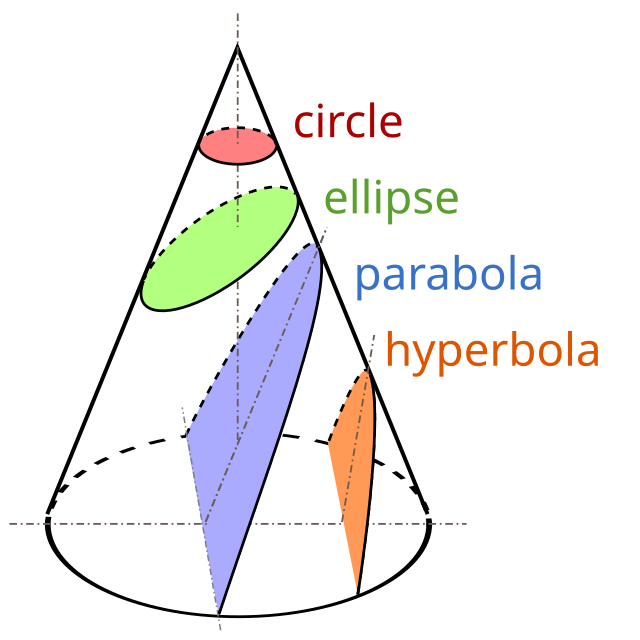
\includegraphics[width=0.4\textwidth]{chapters/chp1_pics/Conic_Sections.svg.png}
\caption{\textit{Conic sections derived from a single-napped cone. The hyperbola includes an additional section, as the intersecting plane extends through the origin to cut both nappes of the cone when there are two present.}}

    \label{fig:conic_sections}
\end{figure}



These curves can all be described by the general quadratic equation in two dimensions:
\[
Ax^2 + Bxy + Cy^2 + Dx + Ey + F = 0,
\]
where \( A, B, C, D, E, F \) are constants. By varying these constants, we generate the different conic sections. \\ \\ A natural question arises: \textit{How can we extend the idea of conic sections to three dimensions?} If conic sections are formed by the intersection of a plane with a cone, what would happen if we instead consider the intersection of a plane with a "generalized" three-dimensional quadratic surface? What kinds of shapes might we discover in three dimensions? These questions lead us to quadric surfaces. \\ \\ In three dimensions, the general equation for a quadric surface is:
\[
Ax^2 + By^2 + Cz^2 + Dxy + Exz + Fyz + Gx + Hy + Iz + J = 0,
\]
where \( A, B, C, D, E, F, G, H, I, J \) are constants. By adjusting these constants, we can produce a variety of surfaces, such as ellipsoids, hyperboloids, and paraboloids. Each surface is a natural extension of the conic sections, generalized to three-dimensional space. One of the most fascinating aspects of quadric surfaces is the diversity of shapes they produce. Why do we get surfaces as different as spheres, hyperboloids, and paraboloids from a single quadratic equation? Are these shapes related to one another? The answer lies in the interplay between the coefficients in the general equation and the symmetry of the surface.

\noindent To understand this, let us focus on the terms in the quadratic equation:
\[
Ax^2 + By^2 + Cz^2 + Dxy + Exz + Fyz + Gx + Hy + Iz + J = 0.
\]

\begin{itemize}
    \item \textbf{Symmetry and Dominance of Quadratic Terms:} The coefficients \( A, B, \) and \( C \) determine the relative ``stretching" or ``shrinking" along the \( x \)-, \( y \)-, and \( z \)-axes. For example, if \( A, B, \) and \( C \) are all positive, the surface is ``elliptical" in nature, producing shapes like spheres or ellipsoids. If one of these coefficients is negative, the surface takes on a "hyperbolic" character.
    
    \item \textbf{Mixed Terms:} The presence of mixed terms like \( Dxy, Exz, \) or \( Fyz \) introduces asymmetry into the surface. These terms ``tilt" the surface or create interactions between axes that result in more complex geometries.

    \item \textbf{Linear Terms:} The linear terms \( Gx, Hy, Iz \) shift the surface in space, altering its position without changing its overall shape.

    \item \textbf{Constant Term:} The constant \( J \) determines whether the surface passes through the origin or is offset.
\end{itemize}

\noindent The diversity of shapes arises from how these terms combine. For example:
\begin{itemize}
    \item A sphere occurs when \( A = B = C \), and all other terms vanish.
    \item An ellipsoid occurs when \( A, B, C > 0 \), but \( A \neq B \neq C \), and all mixed terms vanish.
    \item A hyperboloid arises when one of \( A, B, \) or \( C \) is negative, creating the distinctive ``saddle" or ``double-sheeted" structure.
\end{itemize}

\noindent Mathematically, these surfaces are related because they share the same fundamental structure: all are solutions to quadratic equations in three variables. By varying the coefficients and constants in the equation, we transition smoothly from one surface type to another.


\noindent To visualize why these shapes differ, think of a quadric surface as a collection of cross-sections. For example:
\begin{itemize}
    \item Setting \( z = k \) in the equation of a quadric surface gives a two-dimensional curve (a conic section) in the \( xy \)-plane. As \( k \) varies, these curves ``stack up" to form the three-dimensional surface.
    \item Similarly, setting \( x = k \) or \( y = k \) provides cross-sections in the \( yz \)- and \( xz \)-planes.
\end{itemize}

\noindent By examining these cross-sections, we can see how the different shapes arise:
\begin{itemize}
    \item For an ellipsoid, every cross-section is an ellipse, regardless of the plane.
    \item For a hyperboloid, some cross-sections are hyperbolas, while others are ellipses.
    \item For a paraboloid, cross-sections are parabolas in one direction and ellipses in another.
\end{itemize}

\noindent This perspective highlights the deep connection between conic sections and quadric surfaces: quadric surfaces are essentially ``stacks" of conic sections in three dimensions.

\subsubsection*{Preview of Multivariate Functions}

\noindent While our primary focus here is on the geometric nature of quadric surfaces, these surfaces also serve as important examples of multivariate functions. For instance, the equation of an elliptic paraboloid:
\[
\frac{x^2}{a^2} + \frac{y^2}{b^2} = z
\]
can be interpreted as the graph of the function \( z = f(x, y) \). Similarly, hyperbolic paraboloids and other quadric surfaces appear as graphs of functions with more complex structures.

\noindent Understanding quadric surfaces geometrically will prepare us to study multivariate functions rigorously in future lectures, where we will explore topics like partial derivatives, gradients, and optimization.


\subsection*{The Significance of Quadric Surfaces}

\noindent Quadric surfaces derive their name from the quadratic equations that define them. However, you might wonder: \textit{Why do we add the suffix ``-oid" to names like ellipsoid, paraboloid, and hyperboloid?} The term ``-oid" comes from the Greek word \textit{oides}, meaning ``like" or ``resembling." This suffix reflects the idea that quadric surfaces are three-dimensional analogs of their two-dimensional counterparts, the conic sections. 

\noindent For example:
\begin{itemize}
    \item An \textbf{ellipsoid} is ``like" an ellipse but extends into three dimensions.
    \item A \textbf{paraboloid} is ``like" a parabola but curves in three-dimensional space.
    \item A \textbf{hyperboloid} is ``like" a hyperbola, forming a saddle-shaped or double-sheeted surface in three dimensions.
\end{itemize}

\noindent This connection emphasizes the role of quadric surfaces as natural extensions of conic sections. While conic sections arise as intersections of a plane with a cone in two dimensions, quadric surfaces can be thought of as ``generalized" cones or cylinders in three dimensions.

\noindent \textbf{Why Are Quadric Surfaces Important?} These surfaces form the foundation for multivariate functions because they provide simple models for more complex phenomena. The symmetry inherent in quadric surfaces makes them ideal for representing many physical systems and mathematical problems. Consider the following examples:
\begin{itemize}
    \item \textbf{Paraboloids:} The surface of a satellite dish is a paraboloid, which focuses signals to a single point. Similarly, the shape of a suspension bridge cable under uniform load approximates a paraboloid.
    \item \textbf{Ellipsoids:} The orbits of some planets and the shape of Earth (approximated as an oblate spheroid) can be modeled using ellipsoids.
    \item \textbf{Hyperboloids:} Certain cooling towers, telescopes, and lenses rely on hyperboloids for their structural and optical properties.
\end{itemize}

\noindent Beyond these applications, quadric surfaces are central to \textbf{optimization problems}. They often appear as the contours of multivariate functions, where the geometry of the surface reveals key insights into the behavior of the function. For instance, an elliptic paraboloid can represent a local minimum, while a hyperbolic paraboloid can represent a saddle point.


\subsection*{Equations of Quadric Surfaces}

\noindent Let us first consider the simplest cases of quadric surfaces and slowly generalize to more complex ones. We will examine each surface type systematically, deriving its equation and visualizing its geometry.

\subsubsection*{Ellipsoids}

\noindent An ellipsoid is a natural three-dimensional extension of an ellipse. It is a surface defined by the equation:
\[
\frac{x^2}{a^2} + \frac{y^2}{b^2} + \frac{z^2}{c^2} = 1,
\]
where \( a, b, c > 0 \) are constants that determine the lengths of the semi-axes along the \( x \)-, \( y \)-, and \( z \)-axes, respectively. To understand this equation intuitively, let us set \( z = 0 \). The equation reduces to:
\[
\frac{x^2}{a^2} + \frac{y^2}{b^2} = 1,
\]
which represents an ellipse in the \( xy \)-plane. Similarly, setting \( y = 0 \) gives:
\[
\frac{x^2}{a^2} + \frac{z^2}{c^2} = 1,
\]
an ellipse in the \( xz \)-plane. Thus, the ellipsoid can be thought of as a ``stack" of ellipses in different planes.

\subsubsection*{Hyperboloids}

\noindent A hyperboloid comes in two varieties: one-sheeted and two-sheeted.

\paragraph{One-Sheeted Hyperboloid:} The equation for a one-sheeted hyperboloid is:
\[
\frac{x^2}{a^2} + \frac{y^2}{b^2} - \frac{z^2}{c^2} = 1.
\]
\noindent Here, the negative term (\( -\frac{z^2}{c^2} \)) causes the surface to open outward, creating a ``saddle-like" shape. Setting \( z = 0 \) reduces the equation to:
\[
\frac{x^2}{a^2} + \frac{y^2}{b^2} = 1,
\]
an ellipse in the \( xy \)-plane. However, as \( z \) increases or decreases, the cross-sections remain ellipses but grow larger, giving the hyperboloid its distinctive shape.

\paragraph{Two-Sheeted Hyperboloid:} The equation for a two-sheeted hyperboloid is:
\[
\frac{x^2}{a^2} + \frac{y^2}{b^2} - \frac{z^2}{c^2} = -1.
\]
\noindent This equation is similar to that of the one-sheeted hyperboloid, but here the minus sign on the right-hand side creates two disconnected surfaces, or ``sheets," opening in opposite directions. Setting \( z = 0 \) results in no real solutions, which explains the gap between the two sheets.






\subsubsection*{Elliptic Paraboloid}

\noindent The elliptic paraboloid is defined by the equation:
\[
\frac{x^2}{a^2} + \frac{y^2}{b^2} = z.
\]
\noindent To understand why we call this surface an \textit{elliptic paraboloid}, let us analyze its cross-sections:
\begin{itemize}
    \item Setting \( z = k \), where \( k > 0 \), reduces the equation to:
    \[
    \frac{x^2}{a^2} + \frac{y^2}{b^2} = k,
    \]
    which is the equation of an ellipse in the \( xy \)-plane. As \( z \) increases, these ellipses grow larger, creating a ``bowl-like" shape that opens upwards.
    \item On the other hand, setting \( x = k_1 \) or \( y = k_2 \) (for fixed constants \( k_1, k_2 \)) gives parabolas in the \( yz \)- or \( xz \)-plane, respectively. These parabolas describe how the surface curves along the vertical direction.
\end{itemize}
\noindent The name \textit{elliptic paraboloid} reflects the dual nature of this surface:
\begin{itemize}
    \item The term ``elliptic" comes from the elliptical cross-sections in the \( xy \)-plane.
    \item The term ``paraboloid" signifies that the surface extends like a parabola in the vertical direction.
\end{itemize}
\noindent This combination of elliptical and parabolic characteristics is the hallmark of an elliptic paraboloid.

\subsubsection*{Hyperbolic Paraboloid}

\noindent The hyperbolic paraboloid, often called a ``saddle surface," is defined by the equation:
\[
\frac{x^2}{a^2} - \frac{y^2}{b^2} = z.
\]
\noindent To understand the naming of this surface, let us examine its structure:
\begin{itemize}
    \item Setting \( z = k \) (for any constant \( k \)) reduces the equation to:
    \[
    \frac{x^2}{a^2} - \frac{y^2}{b^2} = k,
    \]
    which represents hyperbolas in the \( xy \)-plane when \( k \neq 0 \). These hyperbolas change orientation depending on the sign of \( k \): 
    \begin{itemize}
        \item For \( k > 0 \), the hyperbolas open along the \( x \)-axis.
        \item For \( k < 0 \), the hyperbolas open along the \( y \)-axis.
    \end{itemize}
    \item When \( z = 0 \), the equation becomes:
    \[
    \frac{x^2}{a^2} - \frac{y^2}{b^2} = 0,
    \]
    which simplifies to two intersecting lines, \( y = \pm \frac{b}{a}x \), in the \( xy \)-plane.
    \item Setting \( x = k_1 \) or \( y = k_2 \) (for fixed constants \( k_1, k_2 \)) gives parabolas in the \( yz \)- or \( xz \)-plane, respectively. These parabolas curve in opposite directions, creating the characteristic "saddle" shape.
\end{itemize}

\noindent The name \textit{hyperbolic paraboloid} reflects the surface's dual nature:
\begin{itemize}
    \item The term ``hyperbolic" comes from the hyperbolic cross-sections in the \( xy \)-plane.
    \item The term ``paraboloid" signifies that the surface contains parabolic cross-sections along the \( xz \)- and \( yz \)-planes.
\end{itemize}

\noindent The hyperbolic paraboloid's unique combination of upward and downward curvature makes it a saddle surface, giving it a distinct role in geometry and multivariable calculus.


\subsubsection*{Cylinders}

\noindent Cylinders are unique among quadric surfaces because they extend infinitely in one direction while maintaining a consistent cross-sectional shape in the other two dimensions. A cylinder can be thought of as the ``extrusion" of a conic section along an axis. The simplest form of a cylinder is the circular cylinder, given by:
\[
x^2 + y^2 = r^2,
\]
where \( r \) is the radius. While this equation might appear two-dimensional, it is not. The apparent ``two-dimensional" nature arises because the equation describes the cross-sectional shape of the cylinder in the \( xy \)-plane when \( z = 0 \). The cylinder itself is three-dimensional, extending infinitely in the \( z \)-direction. Setting \( z = k \) for any \( k \) gives circular cross-sections of radius \( r \) in the \( xy \)-plane at that height. More generally, a cylinder can take on other cross-sectional shapes, such as ellipses or parabolas. For example:
\begin{itemize}
    \item An \textbf{elliptic cylinder} is defined by:
    \[
    \frac{x^2}{a^2} + \frac{y^2}{b^2} = 1,
    \]
    which forms an ellipse in the \( xy \)-plane and extends infinitely in the \( z \)-direction.
    \item A \textbf{parabolic cylinder} is defined by:
    \[
    y = ax^2,
    \]
    which forms a parabola in the \( xy \)-plane and extends infinitely in the \( z \)-direction.
\end{itemize}

\noindent Cylinders are significant because they introduce the idea of surfaces that are not entirely bounded but still exhibit a clear geometric structure. They also help bridge the gap between two-dimensional conic sections and three-dimensional quadric surfaces.


\subsubsection*{Cones}

\noindent A cone is defined by the equation:
\[
\frac{x^2}{a^2} + \frac{y^2}{b^2} = \frac{z^2}{c^2}.
\]
\noindent Setting \( z = k \), where \( k \neq 0 \), reduces the equation to:
\[
\frac{x^2}{a^2} + \frac{y^2}{b^2} = k^2,
\]
an ellipse in the \( xy \)-plane. At \( z = 0 \), the equation reduces to a single point (the vertex of the cone). 


\subsubsection*{Visualization}
The below visual are what these quadric surfaces look like:



\begin{figure}[H]
    \centering
    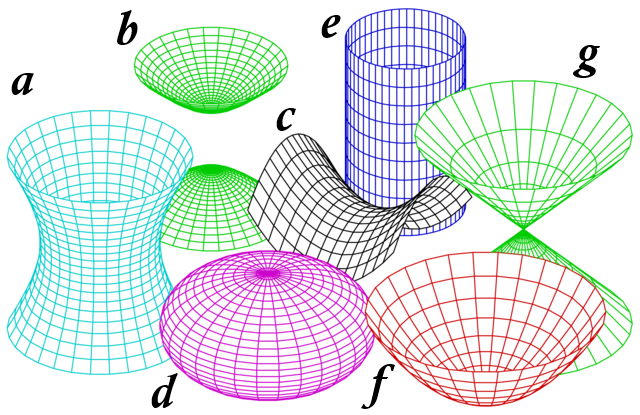
\includegraphics[width=0.8\textwidth]{chapters/chp1_pics/quadric_label.png}
    \caption{\textit{Assorted quadric surfaces.}}
    \label{fig:quadric_surfaces}
\end{figure}

\noindent The labeled surfaces are as follows:
\begin{enumerate}
    \item[a.] \textbf{Hyperboloid of One Sheet:} \( \frac{x^2}{a^2} + \frac{y^2}{b^2} - \frac{z^2}{c^2} = 1 \)
    \item[b.] \textbf{Hyperboloid of Two Sheets:} \( -\frac{x^2}{a^2} - \frac{y^2}{b^2} + \frac{z^2}{c^2} = 1 \)
    \item[c.] \textbf{Hyperbolic Paraboloid:} \( \frac{x^2}{a^2} - \frac{y^2}{b^2} = z \)
    \item[d.] \textbf{Ellipsoid:} \( \frac{x^2}{a^2} + \frac{y^2}{b^2} + \frac{z^2}{c^2} = 1 \)
    \item[e.] \textbf{Cylinder:} \( x^2 + y^2 = r^2 \)
    \item[f.] \textbf{Elliptic Paraboloid:} \( \frac{x^2}{a^2} + \frac{y^2}{b^2} = z \)
    \item[g.] \textbf{Elliptic Cone:} \( \frac{x^2}{a^2} + \frac{y^2}{b^2} - \frac{z^2}{c^2} = 0 \)
\end{enumerate}



\noindent To further explore the concepts of quadric surfaces, let us introduce a Python program that allows you to visualize these surfaces by manipulating their coefficients. By adjusting the parameters \( A, B, C, \) etc., you can observe how the shape and orientation of the surface changes. This hands-on approach helps build intuition about these mathematical objects.


\vspace{1.3em}


\begin{lstlisting}[language=Python]
import numpy as np
import matplotlib.pyplot as plt
from mpl_toolkits.mplot3d import Axes3D

# Define the function for the quadric surface
def quadric_surface(x, y, A, B, C, D, E, F, G, H, I, J):
    return A*x**2 + B*y**2 + C*(x*y) + D*x + E*y + F  # Replace or expand as needed

# Coefficients (students can modify these to observe changes)
A, B, C = 1, 1, 0
D, E, F = 0, 0, -1

# Create a meshgrid for the surface
x = np.linspace(-2, 2, 100)
y = np.linspace(-2, 2, 100)
x, y = np.meshgrid(x, y)

# Compute z-values for the surface
z = quadric_surface(x, y, A, B, C, D, E, F, 0, 0, 0, 0)

# Plot the surface
fig = plt.figure(figsize=(8, 6))
ax = fig.add_subplot(111, projection='3d')
ax.plot_surface(x, y, z, cmap="viridis", alpha=0.8)

# Labels and title
ax.set_xlabel('X-axis')
ax.set_ylabel('Y-axis')
ax.set_zlabel('Z-axis')
ax.set_title('Quadric Surface Visualization')

plt.show()
\end{lstlisting}

\vspace{1.3em}

\noindent \textbf{How to Use:} 
\begin{enumerate}
    \item Copy and paste the code into a Python environment, such as Jupyter Notebook or an IDE.
    \item Experiment with different values of the coefficients \( A, B, C, D, E, F, \) etc., to explore different quadric surfaces (e.g., ellipsoids, hyperboloids, paraboloids).
    \item Observe how the surface changes in response to these adjustments and compare it with the equations we’ve discussed in this lecture.
\end{enumerate}

\noindent This interactive approach not only reinforces your understanding of quadric surfaces but also demonstrates how algebraic changes in the equation correspond to geometric changes in the graph.


\exampleline
\begin{example}
\textbf{Visualizing the Intersection of a Plane and a Quadric Surface}

\noindent Consider the quadric surface given by:
\[
\frac{x^2}{4} + \frac{y^2}{9} - \frac{z^2}{16} = 1,
\]
which is a hyperboloid of one sheet. Let the intersecting plane be defined by \( z = 2 \). Find the resulting curve of intersection.

\begin{solution}

\noindent To find the intersection, substitute \( z = 2 \) into the equation of the hyperboloid:
\[
\frac{x^2}{4} + \frac{y^2}{9} - \frac{(2)^2}{16} = 1.
\]

\noindent Simplify the \( z^2 \) term:
\[
\frac{x^2}{4} + \frac{y^2}{9} - \frac{4}{16} = 1 \quad \implies \quad \frac{x^2}{4} + \frac{y^2}{9} - \frac{1}{4} = 1.
\]

\noindent Rearrange:
\[
\frac{x^2}{4} + \frac{y^2}{9} = \frac{5}{4}.
\]

\noindent Multiply through by 36 (the least common multiple of 4 and 9) to clear the denominators:
\[
9x^2 + 4y^2 = 45.
\]

\noindent This is the equation of an ellipse in the \( xy \)-plane. The plane \( z = 2 \) intersects the hyperboloid to form an ellipse at this height.

\noindent \textbf{Summary:} The curve of intersection between the hyperboloid \( \frac{x^2}{4} + \frac{y^2}{9} - \frac{z^2}{16} = 1 \) and the plane \( z = 2 \) is:
\[
9x^2 + 4y^2 = 45.
\]
This describes an ellipse in the \( xy \)-plane when viewed at \( z = 2 \).

\end{solution}
\end{example}




\exampleline

\begin{example}
\textbf{Classifying a Quadric Surface by Its Equation}

\noindent Given the equation:
\[
\frac{x^2}{9} + \frac{y^2}{4} + \frac{z^2}{16} = 1,
\]
identify the type of quadric surface and describe its geometric properties.

\begin{solution}

\noindent The given equation is of the form:
\[
\frac{x^2}{a^2} + \frac{y^2}{b^2} + \frac{z^2}{c^2} = 1,
\]
where \( a^2 = 9 \), \( b^2 = 4 \), and \( c^2 = 16 \). Since all the terms are positive and equal to 1 on the right-hand side, this is an \textbf{ellipsoid}.

\noindent \textbf{Geometric Properties:}
\begin{itemize}
    \item The center of the ellipsoid is at \( (0, 0, 0) \), as there are no linear terms in \( x, y, \) or \( z \).
    \item The semi-axes of the ellipsoid are aligned with the coordinate axes:
    \[
    a = 3, \quad b = 2, \quad c = 4.
    \]
    \item The semi-axis lengths \( a, b, c \) define the radii of the ellipsoid along the \( x, y, \) and \( z \)-axes, respectively.
\end{itemize}

\noindent \textbf{Summary:} The equation \( \frac{x^2}{9} + \frac{y^2}{4} + \frac{z^2}{16} = 1 \) represents an ellipsoid centered at the origin with semi-axes of lengths 3, 2, and 4 along the \( x, y, \) and \( z \)-axes.

\end{solution}
\end{example}






\exampleline

\begin{example}
\textbf{Finding the Intersection Between a Cylinder and a Plane}

\noindent Consider the cylinder:
\[
x^2 + y^2 = 9,
\]
and the plane \( z = 3x + y \). Find the parametric equations for their intersection.

\begin{solution}

\noindent This example introduces a new technique for working with nonlinear equations. Previously, we dealt with linear parameterizations for lines and planes. Here, we parameterize a \textit{circle} in the \( xy \)-plane, which is inherently nonlinear.  \\ \\ The cylinder is defined by \( x^2 + y^2 = 9 \). This equation represents a circle in the \( xy \)-plane with radius 3. To parameterize the circle, we note that for a unit circle, the coordinates of points on the circle can be written as \( x = \cos t \) and \( y = \sin t \), where \( t \) is the angle swept counterclockwise from the positive \( x \)-axis. Scaling this relationship to a circle of radius \( r \) gives:
\[
x = r \cos t, \quad y = r \sin t,
\]
where \( t \in [0, 2\pi) \) describes the angle around the circle. Substituting \( r = 3 \), we have:
\[
x = 3 \cos t, \quad y = 3 \sin t, \quad t \in [0, 2\pi).
\]
This parameterization allows us to represent all points on the circle in the \( xy \)-plane as \( t \) varies from \( 0 \) to \( 2\pi \).

\noindent The plane \( z = 3x + y \) provides the \( z \)-coordinate for each point of the intersection. Substituting the parameterized values of \( x \) and \( y \) into the plane equation:
\[
z = 3x + y \implies z = 3(3 \cos t) + 3 \sin t = 9 \cos t + 3 \sin t.
\]

\noindent Thus, the parametric equations for the curve of intersection are:
\[
x = 3 \cos t, \quad y = 3 \sin t, \quad z = 9 \cos t + 3 \sin t, \quad t \in [0, 2\pi).
\]

\noindent \textbf{Key Insight:} Nonlinear equations like \( x^2 + y^2 = 9 \) can often be parameterized using trigonometric functions (\( \cos t \) and \( \sin t \)), leveraging their geometric relationship with circles. While the equations may appear two-dimensional initially, the \( z \)-coordinate from the plane adds a third dimension to the curve of intersection, creating a space curve. \\ \\ \textbf{Summary:} The curve of intersection between the cylinder \( x^2 + y^2 = 9 \) and the plane \( z = 3x + y \) is a space curve parameterized by:
\[
x = 3 \cos t, \quad y = 3 \sin t, \quad z = 9 \cos t + 3 \sin t, \quad t \in [0, 2\pi).
\]

\end{solution}
\end{example}
\exampleline


\newpage


\formsdefs{}

\subsection*{Important Vocabulary}
\begin{itemize}
    \item \textbf{Cartesian Coordinates:} A system to define points in three-dimensional space using \((x, y, z)\).
    \item \textbf{Cylindrical Coordinates:} Defined by \((r, \theta, z)\), where \(r\) is the radial distance, \(\theta\) the angle from the positive \(x\)-axis, and \(z\) the height.
    \item \textbf{Spherical Coordinates:} Represented as \((\rho, \theta, \phi)\), where \(\rho\) is the radial distance, \(\theta\) the azimuthal angle, and \(\phi\) the polar angle.
    \item \textbf{Vector:} A quantity with both magnitude and direction, expressed as \(\mathbf{v} = \langle v_x, v_y, v_z \rangle\).
    \item \textbf{Dot Product:} A scalar product of two vectors, given by \(\mathbf{u} \cdot \mathbf{v} = u_x v_x + u_y v_y + u_z v_z\).
    \item \textbf{Cross Product:} A vector perpendicular to two vectors, calculated using the determinant of a \(3 \times 3\) matrix.
    \item \textbf{Parallelepiped:} A six-faced figure formed by three vectors, where its volume is given by the scalar triple product \(|\mathbf{u} \cdot (\mathbf{v} \times \mathbf{w})|\).
\end{itemize}

\subsection*{Key Formulas}
\begin{multicols}{2}
\paragraph{Distance Formula in 3D:}
\[
d = \sqrt{(x_2 - x_1)^2 + (y_2 - y_1)^2 + (z_2 - z_1)^2}
\]

\paragraph{Midpoint Formula:}
\[
M = \left(\frac{x_1 + x_2}{2}, \frac{y_1 + y_2}{2}, \frac{z_1 + z_2}{2}\right)
\]

\paragraph{Direction Cosines:} \index{Direction Cosines}
\[
\begin{aligned}
\cos \alpha &= \frac{u_x}{|\mathbf{u}|}, \quad
\cos \beta = \frac{u_y}{|\mathbf{u}|}, \\
\cos \gamma &= \frac{u_z}{|\mathbf{u}|}
\end{aligned}
\]
where $\cos^2 \alpha + \cos^2 \beta + \cos^2 \gamma = 1$

\paragraph{Angle Between Vectors:} \index{Vector Angle}
\[
\cos \theta = \frac{\mathbf{u} \cdot \mathbf{v}}{|\mathbf{u}||\mathbf{v}|}, \quad
\sin \theta = \frac{|\mathbf{u} \times \mathbf{v}|}{|\mathbf{u}||\mathbf{v}|}
\]

\paragraph{Dot Product:}
\[
\mathbf{u} \cdot \mathbf{v} = u_x v_x + u_y v_y + u_z v_z
\]

\paragraph{Cross Product:}
\begin{align*}
\mathbf{u} \times \mathbf{v} &= \begin{vmatrix}
\mathbf{i} & \mathbf{j} & \mathbf{k} \\
u_x & u_y & u_z \\
v_x & v_y & v_z
\end{vmatrix} \\
&= \mathbf{i}(u_y v_z - u_z v_y) \\
&\quad - \mathbf{j}(u_x v_z - u_z v_x) \\
&\quad + \mathbf{k}(u_x v_y - u_y v_x)
\end{align*}

\paragraph{Parametric Line:} \index{Parametric Line}
\[
\mathbf{r}(t) = \mathbf{P}_0t + \mathbf{P}_1(1-t), \quad t \in [0,1]
\]
or alternatively:
\[
\mathbf{r}(t) = \mathbf{P}_0 + t\mathbf{v}, \quad t \in \mathbb{R}
\]

\paragraph{Volume of a Parallelepiped (Scalar Triple Product):}
\[
\text{Volume} = |\mathbf{u} \cdot (\mathbf{v} \times \mathbf{w})|
\]

\paragraph{Conversion Between Coordinates:}
\begin{itemize}
\item Cartesian to Cylindrical:
\[
\begin{aligned}
r &= \sqrt{x^2 + y^2}, \quad
\theta = \tan^{-1}\left(\frac{y}{x}\right), \\
z &= z
\end{aligned}
\]
\item Cartesian to Spherical:
\[
\begin{aligned}
\rho &= \sqrt{x^2 + y^2 + z^2}, \quad
\theta = \tan^{-1}\left(\frac{y}{x}\right), \\
\phi &= \cos^{-1}\left(\frac{z}{\rho}\right)
\end{aligned}
\]
\item Cylindrical to Cartesian:
\[
\begin{aligned}
x &= r \cos \theta, \quad
y = r \sin \theta, \\
z &= z
\end{aligned}
\]
\item Spherical to Cartesian:
\[
\begin{aligned}
x &= \rho \sin \phi \cos \theta, \quad
y = \rho \sin \phi \sin \theta, \\
z &= \rho \cos \phi
\end{aligned}
\]
\end{itemize}

\paragraph{Plane Equation:}
\[
Ax + By + Cz + D = 0
\]

\paragraph{Line Equation (Parametric Form):}
\[
\mathbf{r}(t) = \mathbf{v} + t \mathbf{d}
\]

\paragraph{Quadratic Surfaces:}
\begin{itemize}
    \item \textbf{Ellipsoid:} \(\frac{x^2}{a^2} + \frac{y^2}{b^2} + \frac{z^2}{c^2} = 1\)
    \item \textbf{Hyperboloid of One Sheet:} \(\frac{x^2}{a^2} + \frac{y^2}{b^2} - \frac{z^2}{c^2} = 1\)
    \item \textbf{Hyperboloid of Two Sheets:} \(-\frac{x^2}{a^2} - \frac{y^2}{b^2} + \frac{z^2}{c^2} = 1\)
    \item \textbf{Elliptic Paraboloid:} \(\frac{x^2}{a^2} + \frac{y^2}{b^2} = z\)
\end{itemize}
\end{multicols}



\newpage

\practice{}

\begin{multicols}{2}

\begin{enumerate}
    % Calculus 1 and 2 Review (10 Questions)
    \item Differentiate the function \( f(t) = t^3 + \sin(t) + e^t \) with respect to \( t \).
    \item Compute the limit \( \lim_{t \to 0} \frac{\sin(t)}{t} \).
    \item Integrate the function \( f(t) = 2t + 3 \) with respect to \( t \).
    \item Find the critical points of \( f(t) = t^4 - 4t^3 + 6t^2 - 4t + 1 \).
    \item Determine the interval of convergence for the power series \( \sum_{n=0}^{\infty} \frac{x^n}{n!} \).
    \item Evaluate the improper integral \( \int_{1}^{\infty} \frac{1}{x^2} \, dx \).
    \item Find the Taylor series of \( e^x \) centered at \( x = 0 \) up to the \( x^3 \) term.
    \item Compute \( \lim_{x \to \infty} \frac{2x^3 - x + 1}{x^3 + 4x^2} \).
    \item Solve the optimization problem: Find the maximum area of a rectangle inscribed under the curve \( y = 4 - x^2 \).
    \item A ladder 10 feet long is leaning against a wall. If the base of the ladder is pulled away from the wall at a rate of 2 feet per second, how fast is the top of the ladder descending when the base is 6 feet from the wall?

    % Three-Dimensional Coordinate Systems (14 Questions)
    \item Convert the rectangular coordinates \( (x, y, z) = (3, -3, 3) \) to spherical coordinates.
    \item Find the rectangular coordinates of the point with cylindrical coordinates \( (r, \theta, z) = \left(2, \dfrac{\pi}{4}, -1\right) \).
    \item Determine the distance between the points \( (2, -1, 4) \) and \( (-3, 5, -2) \) in three-dimensional space.
    \item Express the spherical coordinates \( (\rho, \theta, \phi) = \left(5, \dfrac{\pi}{3}, \dfrac{\pi}{6}\right) \) in rectangular coordinates.
    \item Convert the point \( (x, y, z) = (-4, 4, \sqrt{3}) \) from rectangular to cylindrical coordinates.
    \item Find the midpoint between the points \( (1, 2, 3) \) and \( (-1, -2, -3) \) in three-dimensional space.
    \item Determine the angle between the positive \( x \)-axis and the projection of the vector \( \mathbf{v} = \langle 3, 3, 3 \rangle \) onto the \( xy \)-plane.
    \item Convert the rectangular coordinates \( (0, -5, 5) \) to spherical coordinates.
    \item Find the cylindrical coordinates of the point \( (x, y, z) = (2\sqrt{2}, 2\sqrt{2}, -3) \).
    \item Determine the spherical coordinates of the point \( (x, y, z) = (-2, -2, 2\sqrt{2}) \).
    \item Express the point \( (\rho, \theta, \phi) = \left(6, \dfrac{2\pi}{3}, \dfrac{\pi}{4}\right) \) in rectangular coordinates.
    \item Convert the cylindrical coordinates \( (r, \theta, z) = \left(3, \dfrac{\pi}{6}, 4\right) \) to spherical coordinates.
    \item Find the rectangular coordinates of the point \( (r, \theta, z) = \left(1, \dfrac{\pi}{2}, -2\right) \).
    \item Determine the distance from the origin to the point \( (x, y, z) = (a, b, c) \) in rectangular coordinates.
    \item Convert the point \( (x, y, z) = (0, 0, 0) \) to spherical coordinates.

    % Vectors (19 Questions)
    \item Compute \( |\mathbf{v}| \) for \( \mathbf{v} = \langle 3, -4, 5 \rangle \).
    \item Find the unit vector in the direction of \( \mathbf{v} = \langle -2, 1, 3 \rangle \).
    \item Calculate \( \mathbf{u} \cdot \mathbf{v} \) for \( \mathbf{u} = \langle 1, 2, 3 \rangle \) and \( \mathbf{v} = \langle 4, 0, -1 \rangle \).
    \item Determine \( \mathbf{u} \times \mathbf{v} \) for \( \mathbf{u} = \langle 1, 0, -1 \rangle \) and \( \mathbf{v} = \langle 0, 2, 3 \rangle \).
    \item Find the angle between \( \mathbf{u} = \langle 1, 2, 3 \rangle \) and \( \mathbf{v} = \langle 3, 2, 1 \rangle \).
    \item Show that \( \mathbf{u} = \langle 2, -1, 0 \rangle \) and \( \mathbf{v} = \langle 4, -2, 0 \rangle \) are \textit{linearly dependent} (meaning that one cannot be written as a constant multiple of the other).
    \item Compute the area of the parallelogram spanned by \( \mathbf{u} = \langle 1, 0, 1 \rangle \) and \( \mathbf{v} = \langle 0, 2, 1 \rangle \).
    \item Find a vector orthogonal to both \( \mathbf{u} = \langle 1, -1, 0 \rangle \) and \( \mathbf{v} = \langle 2, 1, -1 \rangle \).
    \item Determine if the vectors \( \mathbf{a} = \langle 3, -1, 2 \rangle \), \( \mathbf{b} = \langle 4, 0, -2 \rangle \), and \( \mathbf{c} = \langle 1, 5, -1 \rangle \) are linearly independent.
    \item Find the projection of \( \mathbf{u} = \langle 4, -2, 1 \rangle \) onto \( \mathbf{v} = \langle 1, 0, 3 \rangle \).
    \item Calculate the scalar triple product \( \mathbf{a} \cdot (\mathbf{b} \times \mathbf{c}) \) for \( \mathbf{a} = \langle 1, 2, 3 \rangle \), \( \mathbf{b} = \langle 4, 5, 6 \rangle \), and \( \mathbf{c} = \langle 7, 8, 9 \rangle \).
    \item Find the volume of the parallelepiped formed by the vectors \( \mathbf{u} = \langle 1, 0, 0 \rangle \), \( \mathbf{v} = \langle 0, 1, 0 \rangle \), and \( \mathbf{w} = \langle 0, 0, 1 \rangle \).
    \item Determine the component of \( \mathbf{a} = \langle 5, 2, -3 \rangle \) along \( \mathbf{b} = \langle 1, -1, 2 \rangle \).
    \item Compute the magnitude of the vector \( \mathbf{w} = \mathbf{u} \times \mathbf{v} \) where \( \mathbf{u} = \langle 2, 3, 4 \rangle \) and \( \mathbf{v} = \langle -1, 0, 1 \rangle \).
    \item Find the angle between the vectors \( \mathbf{a} = \langle 2, -1, 3 \rangle \) and \( \mathbf{b} = \langle 1, 4, -2 \rangle \).
    \item Show that the vectors \( \mathbf{u} = \langle 1, 2, 3 \rangle \), \( \mathbf{v} = \langle 4, 5, 6 \rangle \), and \( \mathbf{w} = \langle 7, 8, 9 \rangle \) are \textit{coplanar} (are all on the same plane).
    \item Calculate the area of the triangle formed by the vectors \( \mathbf{u} = \langle 2, 0, -1 \rangle \) and \( \mathbf{v} = \langle 1, 3, 4 \rangle \).
    \item Find the vector projection of \( \mathbf{a} = \langle 3, -2, 1 \rangle \) onto \( \mathbf{b} = \langle 4, 0, -1 \rangle \).
    \item Determine if the vectors \( \mathbf{u} = \langle 2, 4, 6 \rangle \) and \( \mathbf{v} = \langle -1, -2, -3 \rangle \) are orthogonal.
    \item Compute the cross product \( \mathbf{u} \times \mathbf{v} \) for \( \mathbf{u} = \langle 0, 1, 2 \rangle \) and \( \mathbf{v} = \langle 3, 4, 5 \rangle \).
    \item Find the unit vector perpendicular to the plane defined by \( \mathbf{u} = \langle 1, 2, 3 \rangle \) and \( \mathbf{v} = \langle 4, 5, 6 \rangle \).
\item Determine whether the vectors \( \mathbf{a} = \langle 1, 2, 3 \rangle \), \( \mathbf{b} = \langle 2, 4, 6 \rangle \), and \( \mathbf{c} = \langle 3, 6, 9 \rangle \) are linearly independent or dependent. Linear independence means that none of the vectors can be written as a combination of the others, ie $v_1 \neq k_1 v_2 + k_2 v_3$. If at least one vector can be expressed as a combination of the others, the vectors are linearly dependent.
    \item Calculate the dot product \( \mathbf{u} \cdot \mathbf{v} \) for \( \mathbf{u} = \langle 5, -2, 4 \rangle \) and \( \mathbf{v} = \langle -1, 3, 2 \rangle \).
    \item Find the angle between the vectors \( \mathbf{u} = \langle 7, 0, -5 \rangle \) and \( \mathbf{v} = \langle 4, -3, 2 \rangle \).
    \item Show that the vectors \( \mathbf{u} = \langle 1, 3, -2 \rangle \) and \( \mathbf{v} = \langle 4, -1, 5 \rangle \) are not parallel.
    \item Compute the area of the parallelogram formed by \( \mathbf{u} = \langle 3, -1, 2 \rangle \) and \( \mathbf{v} = \langle -2, 4, 1 \rangle \).
    \item Find a vector orthogonal to \( \mathbf{u} = \langle 2, -3, 1 \rangle \) and \( \mathbf{v} = \langle 4, 0, -2 \rangle \).

    % Lines and Planes in Space (14 Questions)
    \item Find the equation of the line passing through \( (1, 0, -1) \) and \( (2, 3, 4) \).
    \item Determine the equation of the plane containing the points \( (1, 2, 3) \), \( (-1, 0, 4) \), and \( (3, -2, 1) \).
    \item Compute the point of intersection of the line \( \mathbf{r}(t) = \langle 1 + t, 2 - t, 3t \rangle \) with the plane \( x - y + z = 5 \).
    \item Check if the lines \( \mathbf{r}_1(t) = \langle t, 2t, 3t \rangle \) and \( \mathbf{r}_2(s) = \langle 1 + s, 2, 3s \rangle \) are parallel, intersecting, or skew.
    \item Given \( \Pi_1: x + 2y + 3z = 7 \), \( \Pi_2: -2x - y - z = 2 \), and \( \mathbf{r}(t) = \langle 2t, 1 - t, 1 + t \rangle \), determine if \( \mathbf{r}(t) \) intersects both planes. If so, calculate the length of \( \mathbf{r}(t) \) from \( \Pi_1 \) to \( \Pi_2 \).
    \item Find the shortest distance between the line \( \mathbf{r}(t) = \langle t, t, t \rangle \) and the point \( (1, 1, 1) \).
    \item Determine the equation of the line of intersection of the planes \( x + y + z = 1 \) and \( 2x - y + 3z = 4 \).
    \item Find the distance between the parallel planes \( x + 2y + 2z = 5 \) and \( x + 2y + 2z = -3 \).
    \item Find the parametric equations of the line perpendicular to the plane \( 3x - 2y + z = 7 \) and passing through the point \( (2, -1, 4) \).
    \item Determine the angle between the line \( \mathbf{r}(t) = \langle 1 + 2t, 3 - t, 4t \rangle \) and the plane \( 2x - 3y + z = 7 \).
    \item Find the equation of the plane perpendicular to the vector \( \mathbf{n} = \langle 3, -2, 5 \rangle \) and passing through the point \( (2, -1, 4) \).
    \item Compute the intersection curve of the sphere \( x^2 + y^2 + z^2 = 25 \) and the plane \( z = 3 \).
    \item Find the equation of a line that is parallel to the vector \( \mathbf{v} = \langle 2, -1, 3 \rangle \) and passes through the point \( (-1, 4, 2) \).
    \item Determine whether the lines \( \mathbf{r}_1(t) = \langle 1 + t, 2 - t, 3 + 2t \rangle \) and \( \mathbf{r}_2(s) = \langle 4 - s, -1 + s, 5 + s \rangle \) intersect.
    \item Compute the equation of the tangent plane to the surface \( x^2 + 2y^2 + 3z^2 = 6 \) at the point \( (1, 1, 1) \).
    \item Find the line segment of shortest length connecting the lines \( \mathbf{r}_1(t) = \langle t, 2t, 3t \rangle \) and \( \mathbf{r}_2(s) = \langle 1 + s, 2 + s, 3 + s \rangle \).
    \item Determine the parametric equations for the space curve defined by \( x = t \), \( y = \sin(t) \), and \( z = \cos(t) \).
    \item Find the intersection of the hyperboloid \( x^2 - y^2 - z^2 = 4 \) with the plane \( y = 1 \).
    \item Calculate the surface area of the cylinder \( x^2 + y^2 = 9 \) between \( z = 0 \) and \( z = 5 \).
    \item Find the equation of the ellipsoid with semi-axes of lengths 3, 4, and 5 along the \( x \)-, \( y \)-, and \( z \)-axes, respectively.
    \item Derive the Cartesian equation of the paraboloid obtained by rotating the parabola \( z = x^2 \) about the \( z \)-axis.
   \item As we have seen, the parametric equation of a line can be represented as $\mathbf{r}(t) = \mathbf{P}_0t + \mathbf{P}_1(1-t), \quad t \in [0,1]$. If we wanted to change $t$ to go between $0$ and $a \in \mathbb{R}^{+}$, how would our parametric equation change?

    % Quadric Surfaces (5 Questions)
    \item Classify the surface given by \( x^2 + y^2 - z^2 = 1 \).
    \item Write the parametric equations for the intersection of the cylinder \( x^2 + y^2 = 4 \) with the plane \( z = x + y \).
    \item Verify if the surface \( x^2 + y^2 - 4z = 0 \) is an elliptic paraboloid.
    \item Compute the volume enclosed by the sphere \( x^2 + y^2 + z^2 = 4 \) and the plane \( z = 1 \).
    \item Find the equation of the surface generated by rotating \( x = y^2 \) about the \( z \)-axis.

\end{enumerate}

\end{multicols}



\chapter{Vector-Valued Functions and Motion in Space}

\section*{Introduction}

A satellite orbiting Earth, a roller coaster car racing along its track, a baseball arcing through the air---each traces a curve through three-dimensional space. To describe such motion, we need functions that output not a single number but a \textit{position}: a point in space that changes with time. These are \textit{vector-valued functions}.\\ \\
\noindent We have already encountered a special case in Chapter 1, where we described lines in space using parametric equations. Those were linear vector-valued functions---the simplest kind. This chapter extends the idea to general curves, including spirals, helices, and the paths of projectiles. Along the way, we develop the calculus of vector-valued functions: how to differentiate and integrate them, and what those operations mean geometrically.\\ \\
\noindent The key concepts that emerge are \textit{velocity} (the tangent vector to the path), \textit{acceleration} (how velocity changes), \textit{curvature} (how sharply the path bends), and \textit{arc length} (the distance traveled along the curve). Together, these tools let us analyze not just \textit{where} an object is, but \textit{how} it moves---the geometry and physics of motion through space.\\ \\
\noindent At the heart of this chapter is the \textbf{TNB frame}---a moving coordinate system built from three mutually perpendicular vectors (tangent, normal, and binormal) that travels along the curve with the object. If velocity tells us where we are going, curvature tells us how the road is turning, and torsion tells us how it is rising out of the plane. These are not abstract concepts: curvature determines the centripetal force on a car rounding a bend, and torsion describes the twist of a strand of DNA. By the end of this chapter, you will be able to decompose any smooth motion in space into its fundamental geometric components.
\newpage 





\lecture{Vector-Valued Functions} \index{Vector-Valued Functions} \index{Scalar Functions}

Vector-valued functions provide a powerful framework for describing curves, motion, and physical phenomena in three-dimensional space. Prior functions you've seen like $f(x) = x^2$ are technically called scalar functions, mapping a real number to a single real value, whereas vector-valued functions output ordered components that capture both magnitude and direction. Building on the geometric intuition developed in Chapter 1, where we discussed lines as parametric equations, we now revisit those concepts as a foundation and extend them to describe more general curves. This section focuses on parametric equations, the cornerstone of vector-valued functions, and lays the groundwork for their application in analyzing motion and change in space.

\subsection*{Parametric Equations} \index{Parametric Equations}

\noindent In Chapter 1, we described a line in space as the set of points extending in a given direction from a specific starting point. If \( \mathbf{P}_0 = \langle x_0, y_0, z_0 \rangle \) is a fixed point on the line and \( \mathbf{d} = \langle a, b, c \rangle \) is a direction vector, the position of any point on the line can be expressed as:
\[
\mathbf{r}(t) = \mathbf{P}_0 + t\mathbf{d}, \quad t \in \mathbb{R}.
\]
Here:
\begin{itemize}
    \item \( \mathbf{P}_0 \) specifies the starting point of the line.
    \item \( \mathbf{d} \) indicates the direction and orientation of the line.
    \item The parameter \( t \) determines the location along the line: \( t > 0 \) moves in the direction of \( \mathbf{d} \), \( t < 0 \) moves in the opposite direction, and \( t = 0 \) corresponds to the point \( \mathbf{P}_0 \).
\end{itemize}

\noindent This parametric representation makes clear that a line is defined by a starting point and a direction vector, with the parameter \( t \) serving as a simple scalar that scales the direction vector.

\subsubsection*{Generalizing to Parametric Curves}

\noindent The simplicity of the line inspires us to generalize this approach to more complex curves. Instead of restricting each coordinate to vary linearly with \( t \), we allow each coordinate to be an independent function of \( t \). A general parametric curve in three-dimensional space can then be expressed as:
\[
\mathbf{r}(t) = \langle f(t), g(t), h(t) \rangle, \quad t \in I,
\]
where \( f(t), g(t), \) and \( h(t) \) are continuous functions defined on an interval \( I \). These functions describe the evolution of the curve’s \( x \)-, \( y \)-, and \( z \)-coordinates, respectively, as the parameter \( t \) varies. This representation of curves as vector-valued functions allows us to extend the linear model of lines to a broader class of paths, capturing motion and shape in space with remarkable flexibility. \\ \\ 
\textit{Note:} In two dimensions, the parametric equation \( \mathbf{r}(t) = \langle t, f(t) \rangle \) essentially represents the graph of the function \( y = f(x) \). Here, \( t \) serves as both the parameter and the \( x \)-coordinate, making it straightforward to visualize the curve as the usual plot of \( y \) versus \( x \).


\subsubsection*{Common Parametric Curves}

\noindent Consider the following examples to illustrate the generalization from lines to more complex curves:

\begin{itemize}
    \item \textbf{Circle in the \( xy \)-Plane:} A circle of radius \( R \), centered at the origin, can be parameterized as:
    \[
    \mathbf{r}(t) = \langle R \cos(t), R \sin(t), 0 \rangle, \quad t \in [0, 2\pi].
    \]
    Here, \( t \) represents the angle, in radians, that the position vector makes with the positive \( x \)-axis.

    \begin{figure}[H]
        \centering
        \begin{tikzpicture}[scale=2]
            % Axes
            \draw[->] (-1.2, 0) -- (1.2, 0) node[anchor=north] {$x$};
            \draw[->] (0, -1.2) -- (0, 1.2) node[anchor=west] {$y$};
            
            % Circle
            \draw[thick, blue] (0,0) circle (1);
            
            % Label radius
            \draw[dashed] (0,0) -- (1,0) node[midway, anchor=north] {$R$};
        \end{tikzpicture}
        \caption{\textit{Circle in the \( xy \)-plane with radius \( R \).}}
        \label{fig:circle_param}
    \end{figure}

    \item \textbf{Helix:} A helix is a three-dimensional curve that spirals around an axis. For instance, a helix with radius \( R \) and constant upward motion along the \( z \)-axis can be expressed as:
    \[
    \mathbf{r}(t) = \langle R \cos(t), R \sin(t), ct \rangle, \quad t \in \mathbb{R},
    \]
    where \( c \) determines the rate of ascent along the \( z \)-axis.

\tdplotsetmaincoords{60}{110}
    \begin{figure}[H]
        \centering
        \begin{tikzpicture}[tdplot_main_coords, scale=2]
            % Axes
            \draw[->] (0,0,0) -- (1.5,0,0) node[anchor=north east] {$x$};
            \draw[->] (0,0,0) -- (0,1.5,0) node[anchor=north west] {$y$};
            \draw[->] (0,0,0) -- (0,0,2.5) node[anchor=south] {$z$};
            
            % Helix
            \draw[domain=0:720, variable=\t, smooth, samples=200, thick, blue]
                plot ({cos(\t)}, {sin(\t)}, {\t/360});
        \end{tikzpicture}
        \caption{\textit{Helix with radius \( R \) spiraling around the \( z \)-axis.}}
        \label{fig:helix_param}
    \end{figure}

    \item \textbf{Cycloid:} A cycloid is the path traced by a point on the rim of a wheel as it rolls along a straight line. Assuming the wheel has radius \( R \), and it starts rolling from the origin, the parametric equation for the cycloid is:
    \[
    \mathbf{r}(t) = \langle R(t - \sin(t)), R(1 - \cos(t)), 0 \rangle, \quad t \in \mathbb{R}.
    \]
    As the wheel rolls, its center moves horizontally at constant speed (contributing \( Rt \) to \( x \)), while the point on the rim swings in a circle around the center. Subtracting this circular motion from the horizontal translation gives \( x = R(t - \sin t) \), and the vertical position becomes \( y = R(1 - \cos t) \).


    \begin{figure}[H]
        \centering
        \begin{tikzpicture}[scale=1]
            % Axes
            \draw[->] (-1, 0) -- (7, 0) node[anchor=north] {$x$};
            \draw[->] (0, -1) -- (0, 3) node[anchor=west] {$y$};
            
            % Cycloid
            \draw[domain=0:6.3, samples=200, smooth, thick, blue]
                plot ({\x - sin(\x r)}, {1 - cos(\x r)});
        \end{tikzpicture}
        \caption{\textit{Cycloid traced by a point on the rim of a rolling wheel.}}
        \label{fig:cycloid_param}
    \end{figure}

\end{itemize}

\noindent These examples illustrate how allowing the components of \( \mathbf{r}(t) \) to vary independently enables the description of diverse paths in space. The cycloid, for instance, captures a real-world motion, while the helix and circle provide insights into more abstract trajectories.





\subsubsection*{Properties of Parametric Curves}

\noindent Understanding the properties of parametric curves is essential for analyzing their behavior. Here, we explore several key properties:

\begin{itemize}
    \item \textbf{Orientation:} 
    One of the primary advantages of parametric equations is their ability to encode the \textit{orientation} of a curve. The parameter \( t \) determines the direction of traversal. For instance, in the parametric equation of a circle:
    \[
    \mathbf{r}(t) = \langle \cos(t), \sin(t), 0 \rangle, \quad t \in [0, 2\pi],
    \]
    the curve is traversed counterclockwise in the \( xy \)-plane as \( t \) increases. Reversing the parameter (e.g., substituting \( t \to -t \)) reverses the orientation, resulting in clockwise traversal.

    \item \textbf{Smoothness:} 
    A parametric curve \( \mathbf{r}(t) = \langle f(t), g(t), h(t) \rangle \) is \textit{smooth} if its components \( f(t), g(t), h(t) \) are differentiable and \( \mathbf{r}'(t) \neq \mathbf{0} \) for all \( t \) in the interval of interest. Smoothness ensures that the curve has no abrupt changes in direction or cusps.

    \item \textbf{Open and Closed Curves:}
    A parametric curve \( \mathbf{r}(t) \) on \( [a, b] \) is \textit{closed} if \( \mathbf{r}(a) = \mathbf{r}(b) \), meaning the curve returns to its starting point. A circle is a classic example. If the curve does not return to its starting point, it is \textit{open}. This distinction matters in applications such as line integrals, which we will encounter later.
\end{itemize}



\subsubsection*{Applications of Parametric Equations}

\noindent Parametric equations are foundational in physics, engineering, and computer graphics, where they are used to model motion, design structures, and render visual effects. Examples include:

\begin{itemize}
    \item \textbf{Modeling Motion:} The trajectory of a projectile under gravity can be described parametrically as:
    \[
    \mathbf{r}(t) = \langle v_0 \cos(\theta) \, t, \, 0, \, v_0 \sin(\theta) \, t - \tfrac{1}{2} g t^2 \rangle,
    \]
    where \( v_0 \) is the initial velocity, \( \theta \) is the launch angle, and \( g \) is the acceleration due to gravity. Here the \( z \)-axis represents height, consistent with the convention used in Section~2.2.

    \item \textbf{Kinematics of Rigid Bodies:} In robotics, the position and orientation of a robotic arm are described using parametric equations, enabling precise control of movement.

    \item \textbf{Rendering Curves in 3D Graphics:} Parametric equations are used to generate and manipulate curves in computer graphics, such as Bézier curves in animations and CAD design.
\end{itemize}

\noindent As we delve into the calculus of vector-valued functions, the ability to differentiate and integrate parametric equations will allow us to analyze motion and physical systems in unprecedented detail. For instance, consider a particle moving along a winding path. At any instant \( t \), its position \( \mathbf{r}(t) \) is determined by the functions \( f(t), g(t), \) and \( h(t) \). The derivatives of these functions will later help us describe the particle’s velocity and acceleration, revealing insights into its behavior at each point along the curve. With this generalization in place, we are now ready to explore the calculus of vector-valued functions, which provides tools to analyze change and motion along these curves.



\subsection*{Calculus of Vector-Valued Functions}  \index{Vector Calculus}

\noindent Now that we have established the foundation of parametric equations and their representation through vector-valued functions, we move to the calculus of these functions. This section explores the derivatives and integrals of vector-valued functions, tools that enable us to analyze curves and change in space. By extending the familiar principles of single-variable calculus to the vector domain, we unlock a powerful framework for understanding the behavior of dynamic systems.

\subsubsection*{Derivatives of Vector-Valued Functions}

\noindent To begin, let us consider the vector-valued function:
\[
\mathbf{r}(t) = \langle f(t), g(t), h(t) \rangle,
\]
where \( f(t), g(t), \) and \( h(t) \) are differentiable scalar functions. Geometrically, the derivative \( \mathbf{r}'(t) \) is a vector tangent to the curve at the point \( \mathbf{r}(t) \). It points in the direction of increasing \( t \) and its magnitude gives the speed at which the curve is being traced. \ \\
Computationally, the derivative is found component-wise:
\[
\mathbf{r}'(t) = \langle f'(t), g'(t), h'(t) \rangle.
\] \\ \\ Higher derivatives are also defined component-wise. The second derivative of \( \mathbf{r}(t) \) is given by:
\[
\mathbf{r}''(t) = \langle f''(t), g''(t), h''(t) \rangle,
\]
which tells us how the velocity is changing. This relates to the curvature of the path, which we will study in detail in Lecture 3. \\ \\ The concept of component-wise differentiation not only simplifies calculations but also lays the foundation for generalizing change in multidimensional contexts. By treating each coordinate function \( f(t), g(t), h(t) \) independently, we maintain a structured approach to understanding how the entire system evolves. \ \

\noindent Important differentiation rules for vector-valued functions:
\begin{itemize}
\item \textbf{Sum Rule:} \( \frac{d}{dt}[\mathbf{r}_1(t) + \mathbf{r}_2(t)] = \mathbf{r}_1'(t) + \mathbf{r}_2'(t) \)
\item \textbf{Scalar Multiple:} \( \frac{d}{dt}[c \, \mathbf{r}(t)] = c \, \mathbf{r}'(t) \)
\item \textbf{Product Rule (scalar × vector):} \( \frac{d}{dt}[f(t) \, \mathbf{r}(t)] = f'(t) \, \mathbf{r}(t) + f(t) \, \mathbf{r}'(t) \)
\item \textbf{Product Rule (dot product):} \( \frac{d}{dt}[\mathbf{r}_1(t) \cdot \mathbf{r}_2(t)] = \mathbf{r}_1'(t) \cdot \mathbf{r}_2(t) + \mathbf{r}_1(t) \cdot \mathbf{r}_2'(t) \)
\item \textbf{Product Rule (cross product):} \( \frac{d}{dt}[\mathbf{r}_1(t) \times \mathbf{r}_2(t)] = \mathbf{r}_1'(t) \times \mathbf{r}_2(t) + \mathbf{r}_1(t) \times \mathbf{r}_2'(t) \)
\item \textbf{Chain Rule:} \( \frac{d}{dt}[\mathbf{r}(f(t))] = \mathbf{r}'(f(t)) \cdot f'(t) \)
\end{itemize}
\noindent These rules mirror their single-variable counterparts. Note that for the cross product, order matters since the cross product is not commutative.\ \

\exampleline
\begin{example}
Suppose a curve is defined by the vector-valued function:
\[
\mathbf{r}(t) = \langle t^3, \sin(t), e^t \rangle.
\]
Determine whether each component is increasing, decreasing, or concave at \( t = \pi \).
\begin{solution}
To analyze the behavior of each component at \( t = \pi \), we compute the first and second derivatives of \( \mathbf{r}(t) \):
\[
\mathbf{r}'(t) = \langle 3t^2, \cos(t), e^t \rangle, \quad \mathbf{r}''(t) = \langle 6t, -\sin(t), e^t \rangle.
\]

\noindent At \( t = \pi \), we evaluate the derivatives component-wise:
\begin{align*}
    \text{First derivative:} & \quad \mathbf{r}'(\pi) = \langle 3\pi^2, \cos(\pi), e^\pi \rangle = \langle 3\pi^2, -1, e^\pi \rangle, \\
    \text{Second derivative:} & \quad \mathbf{r}''(\pi) = \langle 6\pi, -\sin(\pi), e^\pi \rangle = \langle 6\pi, 0, e^\pi \rangle.
\end{align*}

\noindent Component-wise analysis:
\begin{itemize}
    \item \( x(t) = t^3 \): The first derivative \( 3\pi^2 > 0 \) indicates \( x(t) \) is increasing. The second derivative \( 6\pi > 0 \) confirms \( x(t) \) is concave upward.
    \item \( y(t) = \sin(t) \): The first derivative \( \cos(\pi) = -1 \) indicates \( y(t) \) is decreasing. The second derivative \( -\sin(\pi) = 0 \) suggests no concavity at this point.
    \item \( z(t) = e^t \): The first derivative \( e^\pi > 0 \) indicates \( z(t) \) is increasing. The second derivative \( e^\pi > 0 \) confirms \( z(t) \) is concave upward.
\end{itemize}

\noindent Thus, \( x(t) \) and \( z(t) \) are increasing and concave upward, while \( y(t) \) is decreasing with no concavity at \( t = \pi \).
\end{solution}
\end{example}
\exampleline

\noindent The analysis of derivatives provides a systematic way to study the behavior of vector-valued functions. By extending these principles, we can explore higher-order changes and geometric properties of curves in space.


\subsubsection*{Integrals of Vector-Valued Functions}

\noindent Just as derivatives measure rates of change, integrals of vector-valued functions accumulate quantities over an interval. Given a vector-valued function:
\[
\mathbf{r}(t) = \langle f(t), g(t), h(t) \rangle,
\]
the integral of \( \mathbf{r}(t) \) with respect to \( t \) is defined component-wise:
\[
\int \mathbf{r}(t) \, dt = \langle \int f(t) \, dt, \int g(t) \, dt, \int h(t) \, dt \rangle + \mathbf{C},
\]
where \( \mathbf{C} = \langle C_1, C_2, C_3 \rangle \) is a constant vector of integration. In physical terms, integrating a velocity function \( \mathbf{v}(t) \) recovers a position function \( \mathbf{r}(t) \), with the constant vector encoding the initial position. More generally, if \( \mathbf{a}(t) = \mathbf{r}''(t) \) is given, integrating twice recovers \( \mathbf{r}(t) \), with each step requiring a constant vector determined by initial conditions.



\exampleline
\begin{example}
Let \(\mathbf{F}(t) = \langle 3t^2, 2\sin t, e^{2t} \rangle\) be a vector-valued function defined on the interval \( [0, 1] \).

\begin{enumerate}
    \item Compute the definite integral \(\displaystyle \int_0^1 \mathbf{F}(t) \, dt\).
    \item Verify that \(\displaystyle \int_0^1 \mathbf{F}'(t) \, dt = \mathbf{F}(1) - \mathbf{F}(0)\).
    \item Explain why the Fundamental Theorem of Calculus applies component-wise to vector-valued functions.
\end{enumerate}

\begin{solution}
\begin{enumerate}
    \item To compute the definite integral of \(\mathbf{F}(t)\), we integrate each component separately:
    \[
    \int_0^1 \mathbf{F}(t) \, dt = \left\langle \int_0^1 3t^2 \, dt, \int_0^1 2\sin t \, dt, \int_0^1 e^{2t} \, dt \right\rangle.
    \]
    Compute each integral:

    \textbf{First component:}
    \[
    \int_0^1 3t^2 \, dt = \left[ t^3 \right]_0^1 = 1^3 - 0^3 = 1.
    \]

    \textbf{Second component:}
    \[
    \int_0^1 2\sin t \, dt = -2\cos t \bigg|_0^1 = \left( -2\cos 1 \right) - \left( -2\cos 0 \right) = (-2\cos 1) + 2(1) = 2(1 - \cos 1).
    \]

    \textbf{Third component:}
    \[
    \int_0^1 e^{2t} \, dt = \left[ \frac{1}{2} e^{2t} \right]_0^1 = \frac{1}{2} \left( e^{2} - e^{0} \right) = \frac{1}{2} (e^{2} - 1).
    \]

    Therefore,
    \[
    \int_0^1 \mathbf{F}(t) \, dt = \left\langle 1, \, 2(1 - \cos 1), \, \dfrac{1}{2}(e^{2} - 1) \right\rangle.
    \]

    \item First, compute \(\mathbf{F}'(t)\):
    \[
    \mathbf{F}'(t) = \left\langle \frac{d}{dt} 3t^2, \, \frac{d}{dt} 2\sin t, \, \frac{d}{dt} e^{2t} \right\rangle = \left\langle 6t, \, 2\cos t, \, 2e^{2t} \right\rangle.
    \]
    Then compute the integral of \(\mathbf{F}'(t)\):
    \[
    \int_0^1 \mathbf{F}'(t) \, dt = \left\langle \int_0^1 6t \, dt, \, \int_0^1 2\cos t \, dt, \, \int_0^1 2e^{2t} \, dt \right\rangle.
    \]
    Compute each integral:

    \textbf{First component:}
    \[
    \int_0^1 6t \, dt = \left[ 3t^2 \right]_0^1 = 3(1)^2 - 3(0)^2 = 3.
    \]

    \textbf{Second component:}
    \[
    \int_0^1 2\cos t \, dt = 2\sin t \bigg|_0^1 = 2\sin 1 - 2\sin 0 = 2\sin 1 - 0 = 2\sin 1.
    \]

    \textbf{Third component:}
    \[
    \int_0^1 2e^{2t} \, dt = \left[ e^{2t} \right]_0^1 = e^{2} - e^{0} = e^{2} - 1.
    \]

    Now compute \(\mathbf{F}(1) - \mathbf{F}(0)\):
    \[
    \mathbf{F}(1) = \left\langle 3(1)^2, \, 2\sin 1, \, e^{2(1)} \right\rangle = \left\langle 3, \, 2\sin 1, \, e^{2} \right\rangle.
    \]
    \[
    \mathbf{F}(0) = \left\langle 3(0)^2, \, 2\sin 0, \, e^{2(0)} \right\rangle = \left\langle 0, \, 0, \, 1 \right\rangle.
    \]
    Therefore,
    \[
    \mathbf{F}(1) - \mathbf{F}(0) = \left\langle 3 - 0, \, 2\sin 1 - 0, \, e^{2} - 1 \right\rangle = \left\langle 3, \, 2\sin 1, \, e^{2} - 1 \right\rangle.
    \]
    Comparing the results:
    \[
    \int_0^1 \mathbf{F}'(t) \, dt = \left\langle 3, \, 2\sin 1, \, e^{2} - 1 \right\rangle = \mathbf{F}(1) - \mathbf{F}(0).
    \]
    Thus, we have verified that \(\displaystyle \int_0^1 \mathbf{F}'(t) \, dt = \mathbf{F}(1) - \mathbf{F}(0)\).

    \item The Fundamental Theorem of Calculus states that for a real-valued differentiable function \( f \):
    \[
    \int_a^b f'(t) \, dt = f(b) - f(a).
    \]
    For vector-valued functions, each component is a real-valued function. Therefore, we can apply the Fundamental Theorem of Calculus to each component individually:
    \[
    \int_a^b \mathbf{F}'(t) \, dt = \left\langle \int_a^b F_1'(t) \, dt, \, \int_a^b F_2'(t) \, dt, \, \int_a^b F_3'(t) \, dt \right\rangle \]
\[= \left\langle F_1(b) - F_1(a), \, F_2(b) - F_2(a), \, F_3(b) - F_3(a) \right\rangle = \mathbf{F}(b) - \mathbf{F}(a).
    \]
    This shows that the Fundamental Theorem of Calculus applies component-wise to vector-valued functions because integration and differentiation are performed separately on each real-valued component function.
\end{enumerate}
\end{solution}
\end{example}
\exampleline





\subsection*{Applications of Calculus with Vector-Valued Functions}

\noindent The calculus of vector-valued functions appears throughout science and engineering. Here we highlight two concrete applications:

\begin{itemize}
    \item \textbf{Kinematics:} If \( \mathbf{r}(t) \) gives the position of an object, then \( \mathbf{r}'(t) \) is its velocity and \( \mathbf{r}''(t) \) is its acceleration. Integrating works in reverse: given an acceleration (e.g., \( \mathbf{a}(t) = \langle 0, 0, -g \rangle \) for free-fall near Earth's surface), we integrate once to recover velocity and again to recover position, using initial conditions at each step.

    \item \textbf{Computer Graphics:} Smooth curves in animation and CAD software are often defined as vector-valued functions of a parameter. The derivative \( \mathbf{r}'(t) \) gives the tangent direction at each point, which is used for computing surface normals and orienting objects along a path. Integration of these curves yields arc lengths, which are needed for spacing objects uniformly along a trajectory.
\end{itemize}




\exampleline
\begin{example}
Consider the parametric curve defined by
\[
\mathbf{r}(t) = \langle e^t, e^{-t}, t \rangle, \quad t \in \mathbb{R}.
\]
\begin{enumerate}
    \item Show that this curve lies on the surface defined by \( x y = 1 \).
    \item Find the equation of the tangent line to the curve at the point where \( t = 0 \).
\end{enumerate}
\begin{solution}
\begin{enumerate}
    \item To show that the curve lies on the surface \( x y = 1 \), substitute \( x = e^t \) and \( y = e^{-t} \) into the equation:
    \[
    x y = e^t \cdot e^{-t} = e^{t - t} = e^0 = 1.
    \]
    Therefore, for all \( t \in \mathbb{R} \), the point \( (x, y, z) \) lies on the surface \( x y = 1 \).

    \item The tangent vector to the curve at \( t \) is given by:
    \[
    \mathbf{r}'(t) = \left\langle \frac{d}{dt} e^t, \frac{d}{dt} e^{-t}, \frac{d}{dt} t \right\rangle = \langle e^t, -e^{-t}, 1 \rangle.
    \]
    At \( t = 0 \):
    \[
    \mathbf{r}(0) = \langle e^0, e^{0}, 0 \rangle = \langle 1, 1, 0 \rangle,
    \]
    \[
    \mathbf{r}'(0) = \langle e^0, -e^{0}, 1 \rangle = \langle 1, -1, 1 \rangle.
    \]
    Since we are working in three dimensions, we use the parametric equation of a line:
    \[
    \mathbf{r}(s) = \mathbf{P}_0 + s \mathbf{d},
    \]
    where \( \mathbf{P}_0 \) is a point on the line and \( \mathbf{d} \) is the direction vector of the line.

    In this context:
    \[
    \mathbf{P}_0 = \mathbf{r}(0) = \langle 1, 1, 0 \rangle, \quad \mathbf{d} = \mathbf{r}'(0) = \langle 1, -1, 1 \rangle.
    \]
    Therefore, the equation of the tangent line at \( t = 0 \) is:
    \[
    \mathbf{L}(s) = \mathbf{P}_0 + s \mathbf{d} = \langle 1, 1, 0 \rangle + s \langle 1, -1, 1 \rangle.
    \]
    Simplifying, we obtain:
    \[
    \mathbf{L}(s) = \langle 1 + s, 1 - s, 0 + s \rangle = \langle 1 + s, 1 - s, s \rangle.
    \]
    This parametric equation represents the tangent line to the curve at \( t = 0 \).

    \textbf{Explanation:} In three-dimensional space, lines are described using vector equations. The general form is:
    \[
    \mathbf{r}(s) = \mathbf{P}_0 + s \mathbf{d},
    \]
    where \( \mathbf{P}_0 \) is a fixed point on the line and \( \mathbf{d} \) is a direction vector parallel to the line. The parameter \( s \) allows us to trace every point along the line. In this problem, \( \mathbf{r}(0) \) provides the point of tangency, and \( \mathbf{r}'(0) \) gives the direction of the tangent line, which is why we use them in constructing the equation.
\end{enumerate}
\end{solution}
\end{example}
\exampleline




\newpage








\lecture{Motion Along a Curve}

\noindent Building on our understanding of vector-valued functions and their derivatives, we now turn to the study of motion along a curve. This section explores how the calculus of vector-valued functions is applied to describe physical motion in space. Specifically, we examine how position, velocity, and acceleration work together to describe the behavior of moving objects, using the calculus of vector-valued functions.

\subsection*{Motion Along a Curve} \index{Motion}

\noindent When an object moves along a curve in three-dimensional space, its position at time \( t \) is described by a vector-valued function:
\[
\mathbf{r}(t) = \langle x(t), y(t), z(t) \rangle,
\]
where \( x(t), y(t), \) and \( z(t) \) are the coordinates of the object as functions of time. The path traced by \( \mathbf{r}(t) \) represents the trajectory of the object. Analyzing this motion relies on the concepts of derivatives and integrals to extract information about how the position vector changes over time and to reconstruct paths from rates of change. \\ \\  \textbf{The Velocity Vector} \( \mathbf{v}(t) \) is defined as the derivative of the position vector:
\[
\mathbf{v}(t) = \frac{d\mathbf{r}}{dt} = \langle x'(t), y'(t), z'(t) \rangle.
\]
This vector is tangent to the curve at the point \( \mathbf{r}(t) \), indicating the direction of motion at time \( t \). Its magnitude represents the speed of the object:
\[
|\mathbf{v}(t)| = \sqrt{x'(t)^2 + y'(t)^2 + z'(t)^2}.
\]
The \textit{speed} of the particle is the magnitude of its velocity vector: \( \text{speed} = |\mathbf{v}(t)| \). Speed is a scalar quantity -- it tells us how fast the particle moves but not in which direction.

\noindent Geometrically, the velocity vector connects the rate of change of the coordinates \( x, y, \) and \( z \), capturing the instantaneous direction and rate at which the object moves along the curve. \\ \\ \textbf{The Acceleration Vector} \( \mathbf{a}(t) \) is defined as the derivative of the velocity vector:
\[
\mathbf{a}(t) = \frac{d\mathbf{v}}{dt} = \frac{d^2\mathbf{r}}{dt^2} = \langle x''(t), y''(t), z''(t) \rangle.
\]
The acceleration vector quantifies how the velocity vector changes over time, indicating whether the object is speeding up, slowing down, or changing direction. The magnitude of the acceleration vector:
\[
|\mathbf{a}(t)| = \sqrt{x''(t)^2 + y''(t)^2 + z''(t)^2},
\]
provides the total rate of change of velocity. \\ \\ \textbf{Integrals and Motion Reconstruction:} In addition to derivatives, integrals play a fundamental role in understanding motion. The velocity vector \( \mathbf{v}(t) \) is often given as the rate of change of position, and integrating \( \mathbf{v}(t) \) allows us to reconstruct the position vector:
\[
\mathbf{r}(t) = \int \mathbf{v}(t) \, dt + \mathbf{r}_0,
\]
where \( \mathbf{r}_0 \) is the initial position of the object. Similarly, the acceleration vector \( \mathbf{a}(t) \), if known, can be integrated to recover the velocity:
\[
\mathbf{v}(t) = \int \mathbf{a}(t) \, dt + \mathbf{v}_0,
\]
where \( \mathbf{v}_0 \) is the initial velocity of the object. These integrations reveal how the motion accumulates over time, allowing us to describe both the trajectory and the forces acting on the object. \\ \\ Both velocity and acceleration vectors are essential in understanding the dynamics of motion along a curve. For instance:
\begin{itemize}
    \item If the velocity vector \( \mathbf{v}(t) \) is constant, the object moves in a straight line with uniform speed and direction.
    \item If the acceleration vector \( \mathbf{a}(t) \) is zero, the object moves at constant velocity, tracing a straight line in space.
    \item If \( \mathbf{a}(t) \) is not zero, the motion becomes more complex, involving changes in both speed and direction.
\end{itemize}

\noindent The interplay between \( \mathbf{v}(t) \), \( \mathbf{a}(t) \), and their respective integrals provides insights into real-world motion, such as the trajectories of projectiles or the orbits of celestial bodies. In cases where motion occurs under uniform forces, such as gravity, the integration process enables the reconstruction of entire paths from basic physical laws. These relationships will be expanded upon in subsequent sections, where we explore specific examples and applications of motion in physical systems.\\ \\
\noindent Displacement is a vector representing the net change in position from start to finish. Total distance traveled is a scalar measuring the length of the path. For a round trip back to the starting point, displacement is zero but distance is not.

\exampleline
\begin{example}
Suppose a particle moves along a curve with velocity:
\[
\mathbf{v}(t) = \langle 3t, 4, t^2 \rangle, \quad t \in [0, 2].
\]
Find the displacement of the particle as well as total distance traveled.
\begin{solution}
To find the displacement of the particle, we integrate the velocity vector:
\[
\mathbf{r}(t) = \int \mathbf{v}(t) \, dt = \langle \int 3t \, dt, \int 4 \, dt, \int t^2 \, dt \rangle + \mathbf{r}_0.
\]
Assuming the particle starts at the origin (\( \mathbf{r}_0 = \langle 0, 0, 0 \rangle \)), the components of \( \mathbf{r}(t) \) are computed as follows:
\begin{align*}
    \int 3t \, dt &= \frac{3t^2}{2}, \\
    \int 4 \, dt &= 4t, \\
    \int t^2 \, dt &= \frac{t^3}{3}.
\end{align*}
Thus, the position function is:
\[
\mathbf{r}(t) = \langle \frac{3t^2}{2}, 4t, \frac{t^3}{3} \rangle.
\]

\noindent At \( t = 2 \), the displacement is:
\[
\mathbf{r}(2) = \langle \frac{3(2)^2}{2}, 4(2), \frac{(2)^3}{3} \rangle = \langle 6, 8, \frac{8}{3} \rangle.
\]
This vector gives the particle’s position relative to its starting point. \\ \\ To calculate the total distance traveled, we integrate the speed of the particle, which is the magnitude of the velocity:
\[
|\mathbf{v}(t)| = \sqrt{(3t)^2 + 4^2 + (t^2)^2}.
\]
The total distance is given by:
\[
\int_{0}^{2} |\mathbf{v}(t)| \, dt = \int_{0}^{2} \sqrt{(3t)^2 + 4^2 + (t^2)^2} \, dt.
\]

\noindent Simplifying the expression inside the square root:
\[
|\mathbf{v}(t)| = \sqrt{9t^2 + 16 + t^4}.
\]
Since this integral does not have a simple closed-form solution, numerical methods, such as Simpson's Rule or a computational tool, are typically used to evaluate it.
\end{solution}
\end{example}
\exampleline

\subsection*{Projectile Motion} \index{Projectile Motion}

\noindent A classic example of motion along a curve is projectile motion, where an object is launched with an initial speed \( v_0 \) at an angle \( \theta \) above the horizontal plane. The initial velocity vector is given by:
\[
\mathbf{v}_0 = \langle v_{x0}, v_{y0}, v_{z0} \rangle = \langle v_0 \cos \theta, 0, v_0 \sin \theta \rangle,
\]
assuming motion occurs in the \( xz \)-plane (no motion in the \( y \)-direction). The acceleration due to gravity acts downward along the \( z \)-axis, so the acceleration vector is:
\[
\mathbf{a}(t) = \langle 0, 0, -g \rangle,
\]
where \( g \) is the acceleration due to gravity. Integrating the acceleration vector with respect to time gives the velocity vector:
\[
\mathbf{v}(t) = \int \mathbf{a}(t) \, dt + \mathbf{C}_1 = \langle v_0 \cos \theta, 0, v_0 \sin \theta - gt \rangle,
\]
where \( \mathbf{C}_1 = \mathbf{v}_0 \) is the constant of integration representing the initial velocity. Integrating the velocity vector yields the position vector:
\[
\mathbf{r}(t) = \int \mathbf{v}(t) \, dt + \mathbf{C}_2 = \langle v_0 \cos \theta \, t + x_0, \, y_0, \, v_0 \sin \theta \, t - \tfrac{1}{2} gt^2 + z_0 \rangle,
\]
where \( \mathbf{C}_2 = \langle x_0, y_0, z_0 \rangle \) is the initial position vector.

\vspace{2mm}

\noindent These equations describe the parabolic trajectory of a projectile. The horizontal motion (\( x \)-direction) is uniform, while the vertical motion (\( z \)-direction) is uniformly accelerated due to gravity. \\ \\ The parametric equations for the motion are:
\[
\begin{cases}
x(t) = v_0 \cos \theta \, t + x_0, \\
y(t) = y_0, \\
z(t) = v_0 \sin \theta \, t - \tfrac{1}{2} gt^2 + z_0.
\end{cases}
\]

\noindent To eliminate \( t \) and find the equation of the trajectory, solve for \( t \) from \( x(t) \):
\[
t = \frac{x - x_0}{v_0 \cos \theta}.
\]
\noindent Substitute \( t \) into \( z(t) \):
\[
z = v_0 \sin \theta \left( \frac{x - x_0}{v_0 \cos \theta} \right) - \tfrac{1}{2} g \left( \frac{x - x_0}{v_0 \cos \theta} \right)^2 + z_0.
\]
\noindent Simplify:
\[
z = (x - x_0) \tan \theta - \frac{g (x - x_0)^2}{2 v_0^2 \cos^2 \theta} + z_0.
\]
\noindent This equation represents the parabolic path of the projectile in the \( xz \)-plane.

\subsubsection*{Maximum Height}

\noindent The maximum height \( z_{\text{max}} \) of the projectile can be found by analyzing the vertical motion. The vertical component of velocity is:
\[
v_z(t) = v_0 \sin \theta - gt.
\]
\noindent The maximum height occurs when \( v_z(t) = 0 \):
\[
v_0 \sin \theta - gt_{\text{max}} = 0 \implies t_{\text{max}} = \frac{v_0 \sin \theta}{g}.
\]
\noindent Substitute \( t_{\text{max}} \) into \( z(t) \) to find \( z_{\text{max}} \):
\[
z_{\text{max}} = v_0 \sin \theta \left( \frac{v_0 \sin \theta}{g} \right) - \tfrac{1}{2} g \left( \frac{v_0 \sin \theta}{g} \right)^2 + z_0.
\]
\noindent Simplify:
\[
z_{\text{max}} = \frac{v_0^2 \sin^2 \theta}{g} - \frac{v_0^2 \sin^2 \theta}{2g} + z_0 = \frac{v_0^2 \sin^2 \theta}{2g} + z_0.
\]
\subsubsection*{Angle for Maximum Height}

\noindent The maximum height \( z_{\text{max}} \) depends on \( \sin^2 \theta \). Since \( \sin \theta \) reaches its maximum value at \( \theta = 90^\circ \), the maximum height is achieved when the projectile is launched vertically upward. Therefore, the angle that produces the maximum height is:
\[
\theta_{\text{max\_height}} = 90^\circ.
\]

\subsubsection*{Maximum Range}

\noindent The horizontal range \( R \) of the projectile (assuming it lands at the same vertical position from which it was launched, i.e., \( z = z_0 \)) is found by determining the time of flight \( t_{\text{flight}} \) when \( z(t_{\text{flight}}) = z_0 \):

\noindent Set \( z(t_{\text{flight}}) = z_0 \):
\[
v_0 \sin \theta \, t_{\text{flight}} - \tfrac{1}{2} g t_{\text{flight}}^2 + z_0 = z_0.
\]
\noindent Simplify:
\[
v_0 \sin \theta \, t_{\text{flight}} - \tfrac{1}{2} g t_{\text{flight}}^2 = 0.
\]
\noindent Factor out \( t_{\text{flight}} \neq 0 \):
\[
t_{\text{flight}} = \frac{2 v_0 \sin \theta}{g}.
\]
\noindent The horizontal range is:
\[
R = x(t_{\text{flight}}) - x_0 = v_0 \cos \theta \, t_{\text{flight}} = v_0 \cos \theta \left( \frac{2 v_0 \sin \theta}{g} \right) = \frac{2 v_0^2 \sin \theta \cos \theta}{g}.
\]
\noindent Using the identity \( \sin 2\theta = 2 \sin \theta \cos \theta \):
\[
R = \frac{v_0^2 \sin 2\theta}{g}.
\]


\begin{figure}[H]
    \centering
    \begin{tikzpicture}[x=(330:1cm),y=(30:1cm),z=(90:1cm)]
        % green ground
        \fill [LightGreen] (-1,-1,0) -- (-.5,1,0) -- (11,2,0) -- (11,-2,0) -- cycle;
        \fill[Green] (9,0,0) circle [x radius=1.5, y radius=1];
        % black hole
        \fill[black] (10,0,0) circle [x radius=.1, y radius=.1];
        % red flag
        \draw[Brown, thick, line cap=round] (10,0,0) -- (10,0,1);
        \fill[Red] (10,0,1) -- (9.8,0,0.9) -- (10,0,0.8) -- cycle;
        % yellow sand hill
        \fill[Yellow, shift={(7,0,0)}] 
            plot [domain=0:340, samples=20, smooth cycle, variable=\t] 
                (\t:rnd/16+0.25 and rnd/8+0.75);

        % origin
        \node[below left] {$O$};
        % x-axis
        \draw (0, 0) -- (10, 0) 
            node[midway, yshift=-.8cm, rotate=330] {Distance, \( x \) (m)};
        \draw foreach \i in {2,4,6,8} 
            { (\i, 0) node[below, rotate=330] {\i} -- ++(0, .15) };
        % z-axis
        \draw (0, 0, 0) -- (0, 0, 5) 
            node[pos=.8, xshift=-.8cm, rotate=90] {Height, \( z \) (m)};
        \draw foreach \i in {2,4} 
            { (0, 0, \i) node[left] {\i} -- ++(.15, 0, 0) };

        \foreach \a[evaluate={\v=70; \T=\v*sin(\a)/9.807*2;}] in {10, 20, ..., 80} {
            \draw[x=(330:0.5pt), z=(90:0.5pt), Black, dashed]
                plot [smooth, domain=0:\T, samples=50, variable=\t,
                      mark=*, mark repeat=2, mark size=1.8pt, mark options={fill=white, solid}]
                    (\v*\t*cos \a, 0, -9.807/2*\t^2+\v*\t*sin \a +0.1016) coordinate (end);
            \filldraw[fill=White] (end) circle [radius=1.8pt];
        }
    \end{tikzpicture}
    \caption{\textit{A 3D visualization of projectile motion on a golf course. The ball is launched in a parabolic trajectory, reaching the hole marked by the red flag.}
    \label{fig:golf_course_projectile_motion}}
\end{figure}

\subsubsection*{Angle for Maximum Range}

\noindent The maximum range occurs when \( \sin 2\theta \) is maximized. Since \( \sin 2\theta \) reaches its maximum value of 1 when \( 2\theta = 90^\circ \), i.e., \( \theta = 45^\circ \):
\[
\theta_{\text{max\_range}} = 45^\circ.
\]
\noindent Therefore, to achieve the maximum horizontal range, the projectile should be launched at an angle of \( 45^\circ \).


\exampleline
\begin{example}
A golfer is attempting to hit a golf ball over a sandtrap onto the green. The sandtrap is located between 50 meters and 70 meters from the golfer. The green starts at a distance of 70 meters from the golfer. The golfer can hit the ball with an initial speed of \( v_0 = 45 \) m/s. At what minimum angle \( \theta \) above the horizontal must the golfer hit the ball to ensure the ball clears the sandtrap and lands on the green? Ignore air resistance and assume the ball lands at the same vertical level from which it was hit.

\begin{solution}
To ensure the ball clears the sandtrap and lands on the green, the golfer must hit the ball so that it lands at a horizontal distance \( x \geq 70 \) meters from the starting point. \\ \\ The horizontal range \( R \) of a projectile launched at an angle \( \theta \) with initial speed \( v_0 \) and landing at the same vertical level is given by:

\[
R = \dfrac{v_0^2 \sin 2\theta}{g},
\]

where \( g = 9.8 \, \text{m/s}^2 \) is the acceleration due to gravity.

We need to find the minimum angle \( \theta \) such that \( R \geq 70 \) meters.

\begin{enumerate}
    \item \textbf{Set up the inequality for the range:}

    \[
    R = \dfrac{v_0^2 \sin 2\theta}{g} \geq 70.
    \]

    \item \textbf{Solve for \( \sin 2\theta \):}

    \[
    \sin 2\theta \geq \dfrac{70g}{v_0^2}.
    \]

    Substitute \( v_0 = 45 \, \text{m/s} \) and \( g = 9.8 \, \text{m/s}^2 \):

    \[
    \sin 2\theta \geq \dfrac{70 \times 9.8}{45^2} = \dfrac{686}{2025} \approx 0.338.
    \]

    \item \textbf{Solve for \( 2\theta \):}

    \[
    2\theta \geq \sin^{-1}(0.338).
    \]

    Compute \( \sin^{-1}(0.338) \):

    \[
    2\theta \geq 19.78^\circ.
    \]

    \item \textbf{Solve for \( \theta \):}

    \[
    \theta \geq \dfrac{19.78^\circ}{2} = 9.89^\circ.
    \]

\end{enumerate}

\noindent \textbf{Conclusion:} The golfer must hit the ball at a minimum angle of approximately \( 9.89^\circ \) above the horizontal to ensure the ball clears the sandtrap and lands on the green.

\end{solution}
\end{example}
\exampleline




\subsubsection*{Energy Considerations}

\noindent Energy conservation provides an alternative approach to analyzing projectile motion that avoids solving differential equations directly and can serve as a useful check on our kinematic results.

\noindent The initial kinetic energy \( K \) of the projectile is:
\[
K = \tfrac{1}{2} m v_0^2,
\]
where \( m \) is the mass of the projectile. At the maximum height, the kinetic energy is:
\[
K_{\text{max\_height}} = \tfrac{1}{2} m \left( v_0 \cos \theta \right)^2 = \tfrac{1}{2} m v_0^2 \cos^2 \theta.
\]
\noindent The potential energy increase is:
\[
\Delta U = m g (z_{\text{max}} - z_0) = \tfrac{1}{2} m v_0^2 \sin^2 \theta.
\]
\noindent This shows the conservation of mechanical energy:
\[
K = K_{\text{max\_height}} + \Delta U.
\]

\exampleline
\begin{example}
An object is launched from the origin (\( x_0 = z_0 = 0 \)) with an initial speed \( v_0 = 20 \, \text{m/s} \) at an angle \( \theta = 45^\circ \). 

\begin{enumerate}
    \item Derive the parametric equations for the motion of the object, assuming acceleration due to gravity is \( g = 9.8 \, \text{m/s}^2 \).
    \item Find the maximum height of the object using kinematic equations.
    \item Determine the total time of flight.
    \item Calculate the horizontal range of the projectile.
    \item Using energy considerations, calculate the maximum height the object reaches.
\end{enumerate}

\begin{solution}
\begin{enumerate}
    \item \textbf{Parametric Equations.}
    
    Decompose the initial velocity into horizontal and vertical components:
    
    \[
    v_{x0} = v_0 \cos \theta = 20 \cos 45^\circ = 20 \left( \frac{\sqrt{2}}{2} \right) = 10\sqrt{2} \, \text{m/s},
    \]
    
    \[
    v_{z0} = v_0 \sin \theta = 20 \sin 45^\circ = 20 \left( \frac{\sqrt{2}}{2} \right) = 10\sqrt{2} \, \text{m/s}.
    \]
    
    The parametric equations are:
    
    \[
    x(t) = v_{x0} t = 10\sqrt{2} \, t,
    \]
    
    \[
    z(t) = v_{z0} t - \tfrac{1}{2} g t^2 = 10\sqrt{2} \, t - 4.9 t^2.
    \]
    
    \item \textbf{Maximum Height Using Kinematics.}
    
    The maximum height occurs when the vertical velocity becomes zero:
    
    \[
    v_z(t) = v_{z0} - g t = 0 \implies t_{\text{max}} = \dfrac{v_{z0}}{g} = \dfrac{10\sqrt{2}}{9.8} \approx 1.44 \, \text{s}.
    \]
    
    Substitute \( t_{\text{max}} \) into \( z(t) \):
    
    \[
    \begin{aligned}
    z_{\text{max}} &= 10\sqrt{2} \left( \dfrac{10\sqrt{2}}{9.8} \right) - 4.9 \left( \dfrac{10\sqrt{2}}{9.8} \right)^2 \\
    &= \dfrac{200}{9.8} - 4.9 \left( \dfrac{200}{(9.8)^2} \right) \\
    &= \dfrac{200}{9.8} - \dfrac{100}{9.8} \\
    &= \dfrac{100}{9.8} \approx 10.204 \, \text{m}.
    \end{aligned}
    \]
    
    So, the maximum height is approximately \( 10.2 \, \text{m} \).
    
    \item \textbf{Total Time of Flight.}
    
    The total time is when the projectile returns to \( z = 0 \):
    
    \[
    z(t) = 0 \implies 10\sqrt{2} \, t - 4.9 t^2 = 0.
    \]
    
    Factor out \( t \neq 0 \):
    
    \[
    t \left( 10\sqrt{2} - 4.9 t \right) = 0 \implies t_{\text{total}} = \dfrac{10\sqrt{2}}{4.9} \approx 2.89 \, \text{s}.
    \]
    
    \item \textbf{Horizontal Range.}
    
    The horizontal range is:
    
    \[
    x_{\text{range}} = v_{x0} \times t_{\text{total}} = 10\sqrt{2} \times 2.89 \approx 40.8 \, \text{m}.
    \]
    
    \item \textbf{Maximum Height Using Energy Considerations.}
    
    We will use the conservation of mechanical energy to find \( z_{\text{max}} \).
    
    \begin{enumerate}
        \item \textbf{Initial Kinetic Energy:}
        
        \[
        K_i = \tfrac{1}{2} m v_0^2 = \tfrac{1}{2} m (20)^2 = 200 m.
        \]
        
        \item \textbf{Kinetic Energy at Maximum Height:}
        
        At maximum height, vertical velocity is zero, so:
        
        \[
        K_{\text{max}} = \tfrac{1}{2} m v_{x0}^2 = \tfrac{1}{2} m (10\sqrt{2})^2 = 100 m.
        \]
        
        \item \textbf{Potential Energy at Maximum Height:}
        
        \[
        U_{\text{max}} = m g z_{\text{max}}.
        \]
        
        \item \textbf{Conservation of Mechanical Energy:}
        
        \[
        K_i = K_{\text{max}} + U_{\text{max}}.
        \]
        
        \item \textbf{Solve for \( z_{\text{max}} \):}
        
        \[
        200 m = 100 m + m g z_{\text{max}} \implies m g z_{\text{max}} = 100 m.
        \]
        
        Cancel \( m \) from both sides:
        
        \[
        g z_{\text{max}} = 100 \implies z_{\text{max}} = \dfrac{100}{g} = \dfrac{100}{9.8} \approx 10.204 \, \text{m}.
        \]
        
    \end{enumerate}
    
    \textbf{Conclusion:} The maximum height calculated using energy considerations is approximately \( 10.2 \, \text{m} \), which matches the result obtained using kinematic equations.
    
\end{enumerate}
\end{solution}
\end{example}
\exampleline



\newpage

\lecture{The TNB Frame, Curvature and Torsion} \index{TNB Frame} \index{Curvature} \index{Torsion}

The velocity and acceleration vectors from the previous lecture can be decomposed into components that change speed and components that change direction. To separate these, we need a coordinate system that moves with the object---the TNB frame.\\ \\
\noindent When you ride a roller coaster, you feel forces pushing you into your seat, sideways around turns, and up or down over hills. These three directions---forward along the track, sideways toward the center of a curve, and perpendicular to both---correspond precisely to the tangent, normal, and binormal vectors. The TNB frame consists of these three mutually orthogonal unit vectors, forming a moving coordinate system that evolves along the curve and is tied directly to its geometry.\\ \\
\noindent This section introduces the TNB frame and the two scalar quantities that govern its behavior: \textit{curvature}, which measures how sharply a curve bends, and \textit{torsion}, which measures how much a curve twists out of a plane. Together, these tools give us a complete local description of any smooth space curve.

\subsection*{The TNB Frame}

\noindent In previous sections, we discussed the derivatives of vector-valued functions, which naturally give rise to the tangent vector (\( \mathbf{T}(t) \)), and the normal vector (\( \mathbf{N}(t) \)), which we now define precisely. Building upon this foundation, we now introduce the binormal vector (\( \mathbf{B}(t) \)) to complete the TNB frame. Together, these vectors form an orthonormal basis that evolves along the curve, providing a dynamic coordinate system tied directly to the curve’s intrinsic geometry and motion. \\

\noindent Consider a smooth curve parameterized by a vector-valued function:
\[
\mathbf{r}(t) = \langle x(t), y(t), z(t) \rangle, \quad t \in I,
\]
where \( \mathbf{r}'(t) \neq \mathbf{0} \) for all \( t \). The TNB frame is constructed as follows:
\begin{itemize}
    \item \textbf{Tangent Vector (\( \mathbf{T}(t) \)):} The unit tangent vector is defined as:
    \[
    \mathbf{T}(t) = \frac{\mathbf{r}'(t)}{|\mathbf{r}'(t)|}.
    \]
    It points in the direction of motion, describing the instantaneous direction of the curve at each point.
    \item \textbf{Normal Vector (\( \mathbf{N}(t) \)):} The principal normal vector is defined as:
    \[
    \mathbf{N}(t) = \frac{\mathbf{T}'(t)}{|\mathbf{T}'(t)|}.
    \]
    It quantifies how the curve bends by pointing toward the center of curvature at each point.
    \item \textbf{Binormal Vector (\( \mathbf{B}(t) \)):} The binormal vector is defined by the cross product:
    \[
    \mathbf{B}(t) = \mathbf{T}(t) \times \mathbf{N}(t).
    \]
    It is orthogonal to both \( \mathbf{T}(t) \) and \( \mathbf{N}(t) \), completing the right-handed orthonormal basis.
\end{itemize}

\noindent These vectors collectively form the TNB frame, providing a coordinate system uniquely tied to the geometry of the curve. The evolution of the TNB frame along the curve encodes information about its curvature and torsion. Below is an example of a TNB frame of a parametric curve that is going around a cylinder:

\tikzset
{
  surface/.style={draw=cyan,left color=cyan,fill opacity=0.5},
  top/.style={draw=cyan,fill=cyan!30,fill opacity=0.5,canvas is xy plane at z=4},
  pics/helix/.style 2 args={code=% #1 = initial angle, #2 = final angle
    {\draw[pic actions] plot[domain=#1:#2,samples=0.5*#2-0.5*#1+1] 
      ({1.5*cos(\x)},{1.5*sin(\x)},1.5*\x/180);}}, % Added scaling factor of 1.5
  pics/vectors/.style={code=% #1 = angle
    {\draw[green!50!black,-latex,opacity=0.3] ({1.5*cos(#1)},{1.5*sin(#1)},1.5*#1/180) -- 
      ({0.6*cos(#1)},{0.6*sin(#1)},1.5*#1/180) node[pos=1.5] {$\mathbf{N}$};
     \begin{scope}[shift={({1.5*cos(#1)},{1.5*sin(#1)},1.5*#1/180)},rotate around z=90+#1,canvas is xz plane at y=0]
       \draw[blue!50!black,-latex]    (0,0) --++ ({atan(1/pi)}:1.125) node[pos=1.4] {$\mathbf{T}$};
       \draw[magenta!50!black,-latex] (0,0) --++ ({90+atan(1/pi)}:1.5) node[pos=1.3] {$\mathbf{B}$};
     \end{scope}}}
}

\begin{figure}[H]
    \centering
\begin{tikzpicture}[scale=1, isometric view,rotate around z=180,font=\small,
                    line cap=round,line join=round]
% axes
\draw[-latex] (0,0,0) -- (2,0,0) node[left]  {\strut$x$};
\draw[-latex] (0,0,0) -- (0,2,0) node[right] {\strut$y$};
% helix,   background
\pic[red] {helix={135}{315}};
\pic[red] {helix={495}{675}};
% z-axis,  background
\draw (0,0,0) -- (0,0,4);
% vectors, background
\foreach\i in {270,550}
  \pic {vectors=\i};
% cylinder
\draw[surface] (-45:1.5) arc (-45:135:1.5) --++ (0,0,4) arc (135:-45:1.5) -- cycle; % Scaled cylinder radius
\draw[top] (0,0) circle (1.5); % Scaled top circle radius
% z-axis,  foreground
\draw[-latex] (0,0,4) -- (0,0,5.5) node[above] {$z$};
% helix,   foreground
\pic[red] {helix=  {0}{135}};
\pic[red] {helix={315}{495}};
\pic[red] {helix={675}{720}};
% vectors, foreground
\foreach\i in {30,110}
  \pic {vectors=\i};
\end{tikzpicture}
    \caption{\textit{A TNB Frame on a parametric curve around a scaled cylinder}}
    \label{fig:tnb_example}
\end{figure}

\exampleline
\begin{example}
A particle moves along the space curve:
\[
\mathbf{r}(t) = \langle t, t^2, t^3 \rangle, \quad t \in [0, 2].
\]
Find the TNB frame vectors (\( \mathbf{T}(t), \mathbf{N}(t), \mathbf{B}(t) \)) at \( t = 1 \).

\begin{solution}
\begin{enumerate}
    \item Compute derivatives of \( \mathbf{r}(t) \):
    \[
    \mathbf{r}'(t) = \langle 1, 2t, 3t^2 \rangle, \quad \mathbf{r}'(1) = \langle 1, 2, 3 \rangle, \quad |\mathbf{r}'(1)| = \sqrt{1^2 + 2^2 + 3^2} = \sqrt{14}.
    \]
    \[
    \mathbf{r}''(t) = \langle 0, 2, 6t \rangle, \quad \mathbf{r}''(1) = \langle 0, 2, 6 \rangle.
    \]

    \item Compute \( \mathbf{T}(1) \):
    \[
    \mathbf{T}(t) = \frac{\mathbf{r}'(t)}{|\mathbf{r}'(t)|}, \quad \mathbf{T}(1) = \frac{\langle 1, 2, 3 \rangle}{\sqrt{14}} = \left\langle \frac{1}{\sqrt{14}}, \frac{2}{\sqrt{14}}, \frac{3}{\sqrt{14}} \right\rangle.
    \]

    \item Compute \( \mathbf{N}(1) \):
    Computing \( \mathbf{T}'(t) \) directly requires the quotient rule and can be algebraically involved. An equivalent approach is to subtract from \( \mathbf{r}''(t) \) its component along \( \mathbf{T}(t) \), which gives the same direction as \( \mathbf{T}'(t) \):
    \[
    \mathbf{N}(t) = \frac{\mathbf{r}''(t) - \left( \mathbf{r}''(t) \cdot \mathbf{T}(t) \right)\mathbf{T}(t)}{\left| \mathbf{r}''(t) - \left( \mathbf{r}''(t) \cdot \mathbf{T}(t) \right)\mathbf{T}(t) \right|},
    \]
    compute the dot product:
    \[
    \mathbf{r}''(1) \cdot \mathbf{T}(1) = \langle 0, 2, 6 \rangle \cdot \left\langle \frac{1}{\sqrt{14}}, \frac{2}{\sqrt{14}}, \frac{3}{\sqrt{14}} \right\rangle = \frac{22}{\sqrt{14}}.
    \]
    Subtract:
    \[
    \mathbf{r}''(1) - \left( \mathbf{r}''(1) \cdot \mathbf{T}(1) \right) \mathbf{T}(1) = \langle 0, 2, 6 \rangle - \frac{22}{14} \langle 1, 2, 3 \rangle = \left\langle -\frac{11}{7}, -\frac{8}{7}, \frac{9}{7} \right\rangle.
    \]
    Compute the magnitude:
    \[
    \left| \mathbf{N}_{\text{numerator}} \right| = \sqrt{\left( -\frac{11}{7} \right)^2 + \left( -\frac{8}{7} \right)^2 + \left( \frac{9}{7} \right)^2} = \frac{\sqrt{266}}{7}.
    \]
    Thus:
    \[
    \mathbf{N}(1) = \left\langle -\frac{11}{\sqrt{266}}, -\frac{8}{\sqrt{266}}, \frac{9}{\sqrt{266}} \right\rangle.
    \]

    \item Compute \( \mathbf{B}(1) \):
    Using:
    \[
    \mathbf{B}(1) = \mathbf{T}(1) \times \mathbf{N}(1),
    \]
    compute the cross product:
    \[
    \mathbf{B}(1) = \left\langle \frac{3}{\sqrt{19}}, -\frac{3}{\sqrt{19}}, \frac{1}{\sqrt{19}} \right\rangle.
    \]
\end{enumerate}

\noindent At \( t = 1 \), the TNB frame is:
\[
\begin{aligned}
\mathbf{T}(1) &= \left\langle \frac{1}{\sqrt{14}}, \frac{2}{\sqrt{14}}, \frac{3}{\sqrt{14}} \right\rangle, \\
\mathbf{N}(1) &= \left\langle -\frac{11}{\sqrt{266}}, -\frac{8}{\sqrt{266}}, \frac{9}{\sqrt{266}} \right\rangle, \\
\mathbf{B}(1) &= \left\langle \frac{3}{\sqrt{19}}, -\frac{3}{\sqrt{19}}, \frac{1}{\sqrt{19}} \right\rangle.
\end{aligned}
\]
\end{solution}
\end{example}
\exampleline





\subsection*{Curvature} \index{Curvature}

\noindent Beyond position, velocity, and acceleration, the curvature of a curve provides insights into how sharply the trajectory bends at each point. It quantifies the rate at which the direction of the curve changes as you move along it. Curvature measures the rate at which the tangent direction changes per unit arc length---a straight line has zero curvature, while a tight turn has large curvature.

For a smooth curve defined by the vector-valued function \( \mathbf{r}(t) \), the curvature \( \kappa(t) \) at a point is given by:
\[
\kappa(t) = \frac{|\mathbf{r}'(t) \times \mathbf{r}''(t)|}{|\mathbf{r}'(t)|^3} = \frac{|\mathbf{v}(t) \times \mathbf{a}(t)|}{|\mathbf{v}(t)|^3} = \frac{|\mathbf{T}'(t)|}{|\mathbf{r}'(t)|}
\]
The cross-product formula \( \kappa = |\mathbf{r}' \times \mathbf{r}''| / |\mathbf{r}'|^3 \) is the most commonly used for computation.

Here:
\begin{itemize}
    \item \( \mathbf{r}'(t) \) is the first derivative of \( \mathbf{r}(t) \), representing the velocity vector.
    \item \( \mathbf{r}''(t) \) is the second derivative of \( \mathbf{r}(t) \), representing the acceleration vector.
    \item The cross product \( \mathbf{r}'(t) \times \mathbf{r}''(t) \) captures how rapidly the velocity direction is changing. When velocity and acceleration are parallel (straight-line motion), the cross product is zero and so is the curvature.
\end{itemize}

\noindent In the case of \textbf{plane curves} (curves that lie entirely in a plane), there is a simplified formula for curvature. If the curve is given parametrically by \( \mathbf{r}(t) = \langle x(t), y(t) \rangle \), the curvature \( \kappa(t) \) can be calculated as:
\[
\kappa(t) = \frac{|x'(t) y''(t) - y'(t) x''(t)|}{\left( [x'(t)]^2 + [y'(t)]^2 \right)^{3/2}}
\]
This formula is derived from the general vector formula for curvature by evaluating the cross product and magnitudes in two dimensions. When dealing with a single-variable function \( y = f(x) \), we can consider it as a plane curve by parameterizing it as:
\[
\mathbf{r}(t) = \langle t, f(t) \rangle.
\]
In this case, the derivatives are:
\[
x(t) = t, \quad y(t) = f(t), \quad x'(t) = 1, \quad y'(t) = f'(t), \quad x''(t) = 0, \quad y''(t) = f''(t).
\]
Substituting into the plane curve curvature formula:
\[
\kappa(t) = \frac{|x'(t) y''(t) - y'(t) x''(t)|}{\left( [x'(t)]^2 + [y'(t)]^2 \right)^{3/2}} = \frac{|1 \cdot f''(t) - f'(t) \cdot 0|}{\left( [1]^2 + [f'(t)]^2 \right)^{3/2}} = \frac{|f''(t)|}{\left( 1 + [f'(t)]^2 \right)^{3/2}}.
\]
Since \( x = t \), we can write \( \kappa(x) \) as:
\[
\kappa(x) = \frac{|f''(x)|}{\left( 1 + [f'(x)]^2 \right)^{3/2}}.
\]
This formula gives the curvature of the graph of a function \( y = f(x) \) at any point \( x \). This progression shows how the general formula simplifies under specific conditions, making it easier to compute curvature in various contexts. \\ \\ Curvature has a natural interpretation: it describes how much the direction of the \textbf{tangent vector} \( \mathbf{T}(t) = \dfrac{\mathbf{r}'(t)}{|\mathbf{r}'(t)|} \) changes per unit of \textbf{arc length}. This highlights a critical property of curvature: it is independent of the speed at which the curve is traversed. Whether a particle moves along the curve quickly or slowly, the curvature remains tied solely to the trajectory's geometry. \\ \\ The plane curve curvature formula emphasizes how curvature depends on the rates of change of the components of the curve. The numerator \( x'(t) y''(t) - y'(t) x''(t) \) represents the rate at which the direction is changing, while the denominator normalizes this by the speed to the third power, ensuring that curvature is a geometric property of the curve itself, not dependent on parameterization.

\subsubsection*{Osculating Circles} \index{Osculating Circles}
The osculating circle at a point on the curve is the unique circle that shares the same tangent and curvature as the curve at that point. Its radius \( R \), known as the \textit{radius of curvature}, is inversely proportional to the curvature:
\[
R = \frac{1}{\kappa}.
\]
Intuitively, the osculating circle is the circle that best fits the curve at a given point---like pressing a circular template against the curve until it matches as closely as possible. Tight bends correspond to small osculating circles (large curvature), while gentle bends correspond to large osculating circles (small curvature).

For straight lines, where \( \kappa = 0 \), the radius of curvature is infinite, reflecting the absence of bending. Conversely, for a tightly curved loop, \( \kappa \) is large, and \( R \) is small. The osculating circle provides a geometric representation of curvature, capturing the curve’s local behavior with remarkable accuracy. These ideas are not merely theoretical—they allow for practical analysis of paths and trajectories. For example, in designing smooth transitions in roads or roller coasters, one must ensure that the curvature does not exceed safe limits, as excessive bending introduces significant forces.

\subsubsection*{Motion Context}
Curvature also reflects constraints imposed by motion. Consider a car driving along a curved path. The curvature dictates the centripetal force required to maintain the car’s trajectory. A sharper turn (higher curvature) demands greater centripetal acceleration, which is proportional to \( \kappa v^2 \), where \( v \) is the car's speed. Similarly, in orbital mechanics, the curvature of a planet’s trajectory provides insight into the forces acting upon it. The curvature is directly tied to the balance of gravitational pull and the tangential velocity of the orbiting body. \\ \\ To illustrate the concept of curvature, consider the cubic curve \( \mathbf{r}(t) = \langle t, t^3 - 3t^2 + t - 2 \rangle \). This curve alternates between regions of high and low curvature. At peaks and troughs, where the curve bends most sharply, the curvature is maximized. In contrast, at inflection points, where the curve transitions between bending upward and downward, the curvature diminishes.

\begin{figure}[H]
    \centering
\begin{tikzpicture}
    % First axis for the function f(x)
    \begin{axis}[
        name=primary,
        axis y line*=left,
        axis x line*=bottom,
        xlabel={$x$},
        ylabel={$f(x)$},
        xmin=-1, xmax=4,
        ymin=-10, ymax=20,
        grid=both,
        width=12cm,
        height=8cm,
        legend style={
            at={(0,1.05)}, % Place the legend above the left side of the plot
            anchor=south west,
            cells={align=left},
        },
    ]
        % Plot of f(x)
        \addplot[
            domain=-1:4,
            samples=200,
            blue,
            thick,
        ] {x^3 - 3*x^2 + x - 2};
        \addlegendentry{$f(x)$}
    \end{axis}
    
    % Second axis for the curvature kappa(x)
    \begin{axis}[
        axis y line*=right,
        axis x line=none,
        xmin=-1, xmax=4,
        ymin=0, ymax=5,
        ylabel={$\kappa(x)$},
        width=12cm,
        height=8cm,
        at=(primary.south west),
        anchor=south west,
        legend style={
            at={(1,1.05)}, % Place the legend above the right side of the plot
            anchor=south east,
            cells={align=left},
        },
    ]
        % Plot of curvature kappa(x)
        \addplot[
            domain=-1:4,
            samples=200,
            red,
            dashed,
            thick,
        ] {abs(6*x - 6) / ((1 + (3*x^2 - 6*x + 1)^2)^(1.5))};
        \addlegendentry[
            style={red, dashed, thick}
        ]{$\kappa(x)$}
    \end{axis}
\end{tikzpicture}


    \caption{\textit{A polynomial and its curvature (\(\kappa\)) plotted together. The function is shown in blue, and the curvature is shown in dashed red, with a combined legend for clarity.}}
    \label{fig:fun_curvature}
\end{figure}



\noindent In Figure \ref{fig:fun_curvature}, the plot illustrates:
\begin{itemize}
    \item The function \(f(x)\), shown as a blue solid line, representing a cubic polynomial. It exhibits inflection points where the curvature changes sign, corresponding to transitions between concave up and concave down behavior.
    \item The curvature \(\kappa(x)\), shown as a red dashed line, which has peaks near \(x \approx 0.2\) and \(x \approx 1.8\), with the curvature vanishing at the inflection point \(x = 1\), indicating regions of high curvature.
    \item Low curvature values for \(\kappa(x)\) near \(x = -1\), \(x = 4\), and other regions where \(f(x)\) is nearly linear.
\end{itemize}

\noindent Below is a python snippet that you can use to see a function with its curvature on the same plot.




\vspace{1.3em} \index{Python}


\begin{lstlisting}[language=Python]
import numpy as np
import matplotlib.pyplot as plt

def plot_function_and_curvature(func, x_range, scaling_factor=1):
    # Generate x values
    x = np.linspace(x_range[0], x_range[1], 1000)
    dx = x[1] - x[0]  # Assuming uniform spacing

    # Compute y = f(x)
    y = func(x)

    # First derivative f'(x) using numerical differentiation
    f_prime = np.gradient(y, dx)

    # Second derivative f''(x)
    f_double_prime = np.gradient(f_prime, dx)

    # Compute curvature k = |f''(x)| / (1 + [f'(x)]^2)^(3/2)
    curvature = np.abs(f_double_prime) / (1 + f_prime**2)**1.5
    curvature *= scaling_factor  # Apply scaling if needed

    # Plotting
    fig, ax1 = plt.subplots(figsize=(10, 6))

    # Plot the function on the left y-axis
    color1 = 'tab:blue'
    ax1.set_xlabel('x')
    ax1.set_ylabel('Function', color=color1)
    ax1.plot(x, y, label='Function', color=color1, linewidth=2)
    ax1.tick_params(axis='y', labelcolor=color1)
    ax1.grid(True)

    # Create a second y-axis for the curvature
    ax2 = ax1.twinx()

    color2 = 'tab:red'
    ax2.set_ylabel('Curvature', color=color2)
    ax2.plot(x, curvature, label='Curvature', color=color2, linestyle='--', linewidth=2)
    ax2.tick_params(axis='y', labelcolor=color2)

    # Combine legends
    lines_1, labels_1 = ax1.get_legend_handles_labels()
    lines_2, labels_2 = ax2.get_legend_handles_labels()
    ax1.legend(lines_1 + lines_2, labels_1 + labels_2, loc='upper right')

    plt.title('Function and Curvature')
    plt.show()

# Example usage with a polynomial function
def polynomial_function(x):
    return x**3 - 3*x**2 + x - 2

plot_function_and_curvature(polynomial_function, x_range=(-1, 4))

\end{lstlisting}

\vspace{1.3em}

\exampleline
\begin{example}
An engineer is designing a curved road described by the parametric equations:
\[
\mathbf{r}(t) = \langle t, t^2 \rangle, \quad t \in [0, 5].
\]
\begin{enumerate}
    \item Compute the curvature \( \kappa(t) \) of the road at any point \( t \).
    \item Determine the point along the road where the curvature is maximized within the interval \( t \in [0, 5] \).
    \item Discuss how the curvature affects the design and safety of the road.
\end{enumerate}

\begin{solution}
\begin{enumerate}
    \item First, we identify the components of \( \mathbf{r}(t) \):
    \[
    x(t) = t, \quad y(t) = t^2.
    \]
    Compute the first derivatives:
    \[
    x'(t) = 1, \quad y'(t) = 2t.
    \]
    Compute the second derivatives:
    \[
    x''(t) = 0, \quad y''(t) = 2.
    \]
    The curvature \( \kappa(t) \) for plane curves is given by:
    \[
    \kappa(t) = \frac{|x'(t) y''(t) - y'(t) x''(t)|}{\left( [x'(t)]^2 + [y'(t)]^2 \right)^{3/2}}.
    \]
    Substitute the derivatives:
    \[
    \kappa(t) = \frac{| (1)(2) - (2t)(0) |}{\left( 1^2 + (2t)^2 \right)^{3/2}} = \frac{2}{\left( 1 + 4t^2 \right)^{3/2}}.
    \]
    \item To find where the curvature is maximized, we can analyze \( \kappa(t) \):
    \[
    \kappa(t) = \frac{2}{\left( 1 + 4t^2 \right)^{3/2}}.
    \]
    Since the denominator increases with \( t \), the curvature decreases as \( t \) increases. Therefore, the maximum curvature occurs at \( t = 0 \):
    \[
    \kappa_{\text{max}} = \kappa(0) = \frac{2}{(1 + 0)^{3/2}} = 2.
    \]
    \item \textbf{Implications:}
    \begin{itemize}
        \item \textbf{Design and Safety:} The highest curvature at \( t = 0 \) indicates the sharpest bend in the road occurs at the starting point. High curvature requires careful design to ensure vehicles can navigate the curve safely without skidding or overturning.
        \item \textbf{Speed Limits:} Areas with higher curvature may require lower speed limits to maintain safety, as centripetal acceleration increases with curvature and speed.
        \item \textbf{Banking the Road:} Engineers might design the road with banking (tilting the road towards the center of the curve) at high-curvature sections to counteract lateral acceleration and enhance safety.
        \item \textbf{Driver Comfort:} Gradually decreasing curvature along the road (as \( t \) increases) provides a smoother driving experience, reducing the risk of accidents due to sudden changes in direction.
    \end{itemize}
\end{enumerate}
\end{solution}
\end{example}
\exampleline


\subsection*{Torsion} \index{Torsion}

\noindent While curvature quantifies how sharply a curve bends in space, torsion measures how much the curve deviates from being planar—it captures the twist of a space curve out of the plane of curvature. Torsion is a fundamental concept in the study of space curves, providing insights into the three-dimensional behavior of trajectories. For a smooth curve defined by the vector-valued function \( \mathbf{r}(t) \), the torsion \( \tau(t) \) at a point can also be expressed in terms of the tangent, normal, and binormal vectors. Specifically, the torsion relates to the rate of rotation of the binormal vector \( \mathbf{B} \) as:
\[
\mathbf{B}' = -\tau \mathbf{N},
\]
where \( \mathbf{B}' \) is the derivative of the binormal vector, and \( \mathbf{N} \) is the principal normal vector. This provides an alternative definition for torsion:
\[
\tau(t) = -\mathbf{N} \cdot \mathbf{B}'.
\]
Alternatively, using the derivatives of \( \mathbf{r}(t) \), torsion can be computed as:
\[
\tau(t) = \frac{ \left( \mathbf{r}'(t) \times \mathbf{r}''(t) \right) \cdot \mathbf{r}'''(t) }{ \left| \mathbf{r}'(t) \times \mathbf{r}''(t) \right|^2 }.
\]

\noindent Similarly, as we have done with curvature, if we consider a curve in the form \( \mathbf{r}(t) = \langle t, f(t) \rangle \), we can derive an expression for torsion for any function \( f(t) \). Since a curve that lies entirely in a plane cannot twist out of that plane, we should expect the torsion to be zero. Let us verify this. For such a curve:
\[
\mathbf{r}(t) = \langle t, f(t), 0 \rangle.
\]
The derivatives of \( \mathbf{r}(t) \) are:
\[
\mathbf{r}'(t) = \langle 1, f'(t), 0 \rangle, \quad 
\mathbf{r}''(t) = \langle 0, f''(t), 0 \rangle, \quad 
\mathbf{r}'''(t) = \langle 0, f'''(t), 0 \rangle.
\]
The cross product \( \mathbf{r}'(t) \times \mathbf{r}''(t) \) is:
\[
\mathbf{r}'(t) \times \mathbf{r}''(t) = \langle 0, 0, f''(t) \rangle.
\]
Taking the dot product \( \left( \mathbf{r}'(t) \times \mathbf{r}''(t) \right) \cdot \mathbf{r}'''(t) \):
\[
\left( \mathbf{r}'(t) \times \mathbf{r}''(t) \right) \cdot \mathbf{r}'''(t) = 0.
\]
Finally, the torsion for the curve \( \mathbf{r}(t) = \langle t, f(t), 0 \rangle \) simplifies to:
\[
\tau(t) = 0.
\]

\noindent This result shows that a curve defined entirely in a plane (as \( \mathbf{r}(t) = \langle t, f(t) \rangle \) implies) has zero torsion. Torsion is zero for \textbf{planar curves}, as they do not twist out of their plane. A non-zero torsion, on the other hand, indicates that the curve is three-dimensional, exhibiting a helical or twisting behavior. The torsion \( \tau(t) \) measures the rate at which the curve's osculating plane rotates about the tangent vector \( \mathbf{T}(t) \). This rotation reflects the deviation of the curve from being planar. The relationship between torsion and the behavior of a space curve can be summarized as follows:

\begin{itemize}
    \item A \textbf{zero torsion} implies that the osculating plane is constant---the curve lies entirely within a fixed plane.
    \item A \textbf{positive torsion} indicates a right-handed twist of the curve.
    \item A \textbf{negative torsion} indicates a left-handed twist of the curve.
\end{itemize}

\noindent The sign and magnitude of the torsion provide critical information about the direction and intensity of the twist. This insight is invaluable in applications such as DNA helices, spiral staircases, and other helical structures. For instance:

\textbf{Note:} The following applications use the word ``torsion'' in its engineering sense, which is related to but distinct from the geometric torsion of a curve studied in this course.

\begin{itemize}
    \item \textbf{Torsion in Mechanics:} The stress on a twisted rod or beam is directly related to the applied torque \( T \), the polar moment of inertia \( J \), and the radius \( r \):
    \[ \tau_s = \frac{T r}{J}. \]
    \item \textbf{Helical Springs:} In engineering, torsion helps predict the deformation behavior of springs and coils under load.
    \item \textbf{Oscillatory Motion:} The torsional oscillation frequency \( \omega \) of a system is given by:
    \[ \omega = \sqrt{\frac{C}{I}}, \]
    where \( C \) is the torsional constant, and \( I \) is the moment of inertia.
\end{itemize}

\noindent The interplay between torsion \( \tau(t) \) and curvature \( \kappa(t) \) characterizes the local behavior of a space curve. Together, they describe the curve’s geometry and allow for its reconstruction up to position in space. This is formalized in the \textit{Fundamental Theorem of Space Curves}: A space curve is uniquely determined (up to rigid motions in space) by its curvature \( \kappa(t) \) and torsion \( \tau(t) \), provided that \( \kappa(t) > 0 \). The theorem underlines how torsion complements curvature to provide a full geometric understanding of a curve, aiding in both theoretical studies and practical applications. Below is a parametric curve with its respective curvature and torsion plotted below it:

% Plot of the parametric curve with markers, dotted lines, and projections onto x- and y-axes on the xy-plane
\begin{figure}[H]
    \centering
    \begin{tikzpicture}
        \begin{axis}[
            view={60}{30},
            xlabel={$x$},
            ylabel={$y$},
            zlabel={$z$},
            xmin=-1.5, xmax=1.5,
            ymin=-1.5, ymax=1.5,
            zmin=-1.5, zmax=1.5,
            axis lines=center,
            ticks=none,
            width=12cm,
            height=10cm,
            grid=both,
            trig format=rad,
        ]
            % Plot of the parametric curve
            \addplot3[
                domain=0:12.5664,
                samples=200,
                samples y=0,
                blue,
                thick,
            ] (
                {cos(x)},
                {sin(x)},
                {sin(2*x)}
            );
            
            % Maxima and minima points
            \def\maxima{pi/4, 5*pi/4, 9*pi/4}
            \def\minima{3*pi/4, 7*pi/4, 11*pi/4}
            
            % Markers at maxima (blue dots) and projections
            \foreach \t in \maxima {
                \pgfmathsetmacro{\x}{cos(\t)}
                \pgfmathsetmacro{\y}{sin(\t)}
                \pgfmathsetmacro{\z}{sin(2*\t)}
                \addplot3[
                    only marks,
                    mark=*,
                    mark options={blue},
                ] coordinates {
                    (\x,\y,\z)
                };
                % Dotted line down to xy-plane
                \addplot3[
                    dashed,
                    blue,
                ] coordinates {
                    (\x,\y,\z)
                    (\x,\y,0)
                };
                % Dotted line along x to x-axis on xy-plane
                \addplot3[
                    dashed,
                    blue,
                ] coordinates {
                    (\x,\y,0)
                    (0,\y,0)
                };
                % Dotted line along y to y-axis on xy-plane
                \addplot3[
                    dashed,
                    blue,
                ] coordinates {
                    (\x,\y,0)
                    (\x,0,0)
                };
            }
            
            % Markers at minima (red dots) and projections
            \foreach \t in \minima {
                \pgfmathsetmacro{\x}{cos(\t)}
                \pgfmathsetmacro{\y}{sin(\t)}
                \pgfmathsetmacro{\z}{sin(2*\t)}
                \addplot3[
                    only marks,
                    mark=*,
                    mark options={red},
                ] coordinates {
                    (\x,\y,\z)
                };
                % Dotted line down to xy-plane
                \addplot3[
                    dashed,
                    red,
                ] coordinates {
                    (\x,\y,\z)
                    (\x,\y,0)
                };
                % Dotted line along x to x-axis on xy-plane
                \addplot3[
                    dashed,
                    red,
                ] coordinates {
                    (\x,\y,0)
                    (0,\y,0)
                };
                % Dotted line along y to y-axis on xy-plane
                \addplot3[
                    dashed,
                    red,
                ] coordinates {
                    (\x,\y,0)
                    (\x,0,0)
                };
            }
            
            % Draw grid lines on the xy-plane
            \foreach \x in {-1.5,-1.2,...,1.5} {
                \addplot3[
                    gray!50,
                    thin,
                ] coordinates {
                    (\x,-1.5,0)
                    (\x,1.5,0)
                };
            }
            \foreach \y in {-1.5,-1.2,...,1.5} {
                \addplot3[
                    gray!50,
                    thin,
                ] coordinates {
                    (-1.5,\y,0)
                    (1.5,\y,0)
                };
            }
        \end{axis}
    \end{tikzpicture}
    \caption{\textit{Parametric curve $\mathbf{r}(t) = \langle \cos t, \sin t, \sin 2t \rangle$ with markers at local maxima (blue) and minima (red) of $z(t)$, and dotted lines indicating projections onto the $xy$-plane and x- and y-axes.}}
    \label{fig:parametric_curve}
\end{figure}



\begin{figure}[H]
    \centering
\begin{tikzpicture}
    % First axis for curvature
    \begin{axis}[
        name=primary,
        axis y line=left,
        axis x line=bottom,
        xlabel={$t$},
        ylabel={Curvature $\kappa(t)$},
        ylabel style={
            align=center,
            yshift=0.0cm,
        },
        xmin=0, xmax=12.5664,
        ymin=0, ymax=1.5,
        grid=both,
        width=12cm,
        height=8cm,
        legend style={
            at={(0,1.05)},
            anchor=south west,
            cells={align=left},
        },
    ]
        % Plot of curvature using degrees
        \addplot[
            domain=0:12.5664,
            samples=500,
            blue,
            thick,
        ] {
            sqrt(sin(deg(2*x))^2 + 1) / ((1 + 4 * cos(deg(2*x))^2)^(1.5))
        };
        \addlegendentry{$\kappa(t)$ (Curvature)}
    \end{axis}
    
    % Second axis for torsion
    \begin{axis}[
        axis y line=right,
        axis x line=none,
        xlabel={$t$},
        ylabel={Torsion $\tau(t)$},
        ylabel style={
            align=center,
            yshift=0.0cm,
        },
        xmin=0, xmax=12.5664,
        ymin=-2, ymax=2,
        width=12cm,
        height=8cm,
        at=(primary.south west),
        anchor=south west,
        legend style={
            at={(1,1.05)},
            anchor=south east,
            cells={align=left},
        },
    ]
        % Plot of torsion using degrees
        \addplot[
            domain=0:12.5664,
            samples=500,
            red,
            dashed,
            thick,
        ] {
            -2 * cos(deg(2*x)) / (sin(deg(2*x))^2 + 1)
        };
        \addlegendentry{$\tau(t)$ (Torsion)}
    \end{axis}
\end{tikzpicture}

    \caption{\textit{Curvature $\kappa(t)$ (solid blue) and torsion $\tau(t)$ (dashed red) for the parametric curve $\mathbf{r}(t) = \langle \cos t, \sin t, \sin 2t \rangle$.}
    \label{fig:curvature_torsion}}
\end{figure}




\noindent The parametric curve in Figure \ref{fig:curvature_torsion} illustrates how curvature and torsion vary along the curve, embodying the concept of torsion in a tangible form.

\subsubsection*{Motion Context}

In the context of motion, torsion affects the angular momentum of a particle moving along a space curve. The torsion determines how the plane of motion rotates, influencing gyroscopic effects and the stability of the motion. In designing roller coasters or space trajectories, engineers must account for torsion to ensure comfort and structural integrity.

\vspace{1.3em}

\exampleline
\begin{example}
A particle moves along the space curve defined by:
\[
\mathbf{r}(t) = \langle \cos(t),\ \sin(t),\ t \rangle, \quad t \in [0, 2\pi].
\]
\begin{enumerate}
    \item Compute the torsion \( \tau(t) \) of the curve at any point \( t \).
    \item Evaluate the torsion at \( t = \frac{\pi}{2} \).
    \item Interpret the significance of the torsion for this curve.
\end{enumerate}

\begin{solution}
\begin{enumerate}
    \item \textbf{Compute \( \tau(t) \):}

    First, compute the derivatives:

    \textbf{First derivative} \( \mathbf{r}'(t) \):
    \[
    \mathbf{r}'(t) = \langle -\sin(t),\ \cos(t),\ 1 \rangle.
    \]

    \textbf{Second derivative} \( \mathbf{r}''(t) \):
    \[
    \mathbf{r}''(t) = \langle -\cos(t),\ -\sin(t),\ 0 \rangle.
    \]

    \textbf{Third derivative} \( \mathbf{r}'''(t) \):
    \[
    \mathbf{r}'''(t) = \langle \sin(t),\ -\cos(t),\ 0 \rangle.
    \]

    Compute the cross product \( \mathbf{r}'(t) \times \mathbf{r}''(t) \):
    \[
    \begin{aligned}
    \mathbf{r}'(t) \times \mathbf{r}''(t) &= \left| \begin{array}{ccc}
    \mathbf{i} & \mathbf{j} & \mathbf{k} \\
    -\sin(t) & \cos(t) & 1 \\
    -\cos(t) & -\sin(t) & 0 \\
    \end{array} \right| \\
    &= \langle \sin(t),\ -\cos(t),\ 1 \rangle.
    \end{aligned}
    \]

    Compute the magnitude:
    \[
    \left| \mathbf{r}'(t) \times \mathbf{r}''(t) \right| = \sqrt{ \sin^2(t) + \cos^2(t) + 1^2 } = \sqrt{1 + 1} = \sqrt{2}.
    \]

    Compute the dot product \( \left( \mathbf{r}'(t) \times \mathbf{r}''(t) \right) \cdot \mathbf{r}'''(t) \):
    \[
    \begin{aligned}
    \left( \mathbf{r}'(t) \times \mathbf{r}''(t) \right) \cdot \mathbf{r}'''(t) &= \langle \sin(t),\ -\cos(t),\ 1 \rangle \cdot \langle \sin(t),\ -\cos(t),\ 0 \rangle \\
    &= \sin^2(t) + (-\cos(t))^2 + 1 \cdot 0 \\
    &= \sin^2(t) + \cos^2(t) + 0 = 1.
    \end{aligned}
    \]

    Therefore, the torsion is:
    \[
    \tau(t) = \frac{1}{ \left( \sqrt{2} \right)^2 } = \frac{1}{2}.
    \]

    \item \textbf{Evaluate \( \tau\left( \dfrac{\pi}{2} \right) \):}

    Since \( \tau(t) \) is constant and equals \( \dfrac{1}{2} \), we have:
    \[
    \tau\left( \dfrac{\pi}{2} \right) = \frac{1}{2}.
    \]

    \item \textbf{Interpretation:}

    The curve \( \mathbf{r}(t) = \langle \cos(t),\ \sin(t),\ t \rangle \) describes a circular helix with radius 1 and constant upward pitch. The constant torsion \( \tau = \dfrac{1}{2} \) indicates that the curve twists uniformly in space. The positive value signifies a right-handed helix. The constant curvature and torsion reflect the uniform bending and twisting of the helix, characterizing its geometric properties completely.
\end{enumerate}
\end{solution}
\end{example}
\exampleline





\newpage


\lecture{Arc Length and Reparameterization} \index{Arc Length} \index{Reparameterization}

\noindent The concept of arc length is fundamental in calculus and geometry, providing a measure of the distance along a curve. Understanding how to compute arc length is essential for analyzing the properties of curves in various coordinate systems, including Cartesian, parametric, and polar coordinates. Additionally, reparameterizing curves by arc length simplifies many problems in differential geometry and physics by providing a natural parameterization that relates directly to the geometry of the curve.

\subsection*{Computing Arc Length}

\noindent To derive the formula for arc length, consider a smooth curve \( C \) in the plane defined by the function \( y = f(x) \), where \( x \) ranges from \( a \) to \( b \). We can approximate the curve by partitioning the interval \( [a, b] \) into \( n \) subintervals and connecting consecutive points with straight line segments. The length \( \Delta s_i \) of each segment is approximately:

\[
\Delta s_i \approx \sqrt{ \Delta x_i^2 + \Delta y_i^2 } = \sqrt{ (\Delta x_i)^2 + [f'(x_i^*) \Delta x_i]^2 } = \Delta x_i \sqrt{ 1 + [f'(x_i^*)]^2 },
\]

\noindent where \( x_i^* \) is some point in the \( i \)-th subinterval.  Note that we replace the finite difference \( (\Delta y_i)^2 \) with the derivative \( f'(x_i^*) \) multiplied by the finite difference \( \Delta x_i \), following the Mean Value Theorem. This substitution simplifies the expression and emphasizes the relationship between the derivative and the arc length formula. 

\begin{figure}[H]
    \centering
    \begin{tikzpicture}[scale=1.0]
        % Draw the curve y = sin(x/4) + 2
        \draw[thick, domain=0:8, smooth, variable=\x, blue] plot ({\x}, {sin(deg(\x/4)) + 2});
        
        % Points on the curve
        \coordinate (A) at (2, {sin(deg(2/4)) + 2});
        \coordinate (B) at (4, {sin(deg(4/4)) + 2});
        
        % Projection of B onto the horizontal line at y = y(A)
        \coordinate (B_proj) at (4, {sin(deg(2/4)) + 2});
        
        % Draw the triangle
        \draw[red, thick] (A) -- (B) -- (B_proj) -- cycle;
        
        % Deltas
        \draw[-] (A) -- (B) node[midway, above] {$\Delta s$};
        \draw[-] (B_proj) -- (B) node[midway, right] {$\Delta y$};
        \draw[-] (A) -- (B_proj) node[midway, below] {$\Delta x$};
        
        % Axes
        \draw[->] (-0.5,0) -- (9,0) node[right] {$x$};
        \draw[->] (0,-0.5) -- (0,4) node[above] {$y$};
        
        % Labels for points
        \filldraw[black] (A) circle (1pt) node[below left] {$(x, y)$};
        \filldraw[black] (B) circle (1pt) node[above right] {$(x+\Delta x, y+\Delta y)$};
        
        % Dashed lines to show projection onto y = y(A)
        \draw[dashed] (B) -- (B_proj);
        
        % Optional grid
        % \draw[step=1cm, gray, very thin] (-0.5,-0.5) grid (9,4);
    \end{tikzpicture}
    \caption{Approximating the arc length of a curve using a right triangle with \( \Delta s \) as the hypotenuse, \( \Delta x \) as the base, and \( \Delta y \) as the height.}
    \label{fig:arc_length_approximation_single_triangle}
\end{figure}


\noindent Next, summing over all segments, the total approximate arc length \( S \) is:

\[
S \approx \sum_{i=1}^{n} \Delta s_i = \sum_{i=1}^{n} \Delta x_i \sqrt{ 1 + [f'(x_i^*)]^2 }.
\]

\noindent Taking the limit as \( n \to \infty \) and \( \Delta x_i \to 0 \), the sum becomes an integral:

\[
S = \int_{a}^{b} \sqrt{ 1 + [f'(x)]^2 } \, dx.
\]

\noindent The integrand \( \sqrt{ 1 + [f'(x)]^2 } \) represents the differential arc length element \( ds \), so we can express the arc length as:

\[
S = \int_{C} ds = \int_{a}^{b} \sqrt{ 1 + [f'(x)]^2 } \, dx.
\]

\noindent For a closed curve $C$, we may also introduce the notation to be later used:

\[
S = \oint_{C} ds = \int_{a}^{b} \sqrt{ 1 + [f'(x)]^2 } \, dx.
\]

\noindent Similarly, for a curve defined parametrically by \( x = x(t) \) and \( y = y(t) \), with \( t \) ranging over \( [\alpha, \beta] \), we can derive the arc length formula starting from the Cartesian form \( ds = \sqrt{1 + [f'(x)]^2} \, dx \). Using the relationships \( dx = x'(t) \, dt \) and \( dy = y'(t) \, dt \), and noting that \( f'(x) = \frac{dy}{dx} = \frac{y'(t)}{x'(t)} \), substituting and simplifying gives:

\[
ds = \sqrt{ [x'(t)]^2 + [y'(t)]^2 } \, dt.
\]

\noindent Thus, the arc length \( S \) is:

\[
S = \int_{C} ds = \int_{\alpha}^{\beta} \sqrt{ [x'(t)]^2 + [y'(t)]^2 } \, dt.
\]

\noindent Extending this to three-dimensional space, where the curve is given by \( \mathbf{r}(t) = \langle x(t), y(t), z(t) \rangle \), the differential arc length element becomes:

\[
ds = \sqrt{ [x'(t)]^2 + [y'(t)]^2 + [z'(t)]^2 } \, dt = \left| \mathbf{r}'(t) \right| \, dt.
\]

\noindent Therefore, the arc length \( S \) is:

\[
S = \int_{C} ds = \int_{\alpha}^{\beta} \left| \mathbf{r}'(t) \right| \, dt.
\]

\noindent A typical application of arc length is sector length that you may have studied in your Pre-Calculus class:

\begin{figure}[H]
    \centering
    \begin{tikzpicture}
        % Define the circle
        \draw[thick] (0,0) circle (2);
        
        % Draw radius lines
        \draw[thick] (0,0) -- (2,0);
        \draw[thick] (0,0) -- ({2*cos(45)},{2*sin(45)}) node[midway, above left] {Radius};
        
        % Highlight the arc length
        \draw[very thick, red] (2,0) arc[start angle=0, end angle=45, radius=2] 
            node[midway, above right, text=black] {Arc Length};
        
        % Add angle
        \draw[->] (1.2,0) arc[start angle=0, end angle=45, radius=1.2];
        \node at (1.5,0.5) {$\theta$};
        
        % Add center point
        \filldraw (0,0) circle (2pt) node[below] {Center};
        
        % Label circle
        \node at (0,-3.5) {Circle with radius $r$};
    \end{tikzpicture}
    \caption{A circular sector with radius \( r \), central angle \( \theta \), and arc length \( L = r\theta \).}
\end{figure}


\subsubsection*{Arc Length in Polar Coordinates} \index{Polar Coordinate Arc Length}

\noindent In polar coordinates, where a curve is defined by \( r = r(\theta) \), the differential arc length element is derived using the relationship between Cartesian and polar coordinates:

\[
ds = \sqrt{ \left( \frac{dx}{d\theta} \right)^2 + \left( \frac{dy}{d\theta} \right)^2 } \, d\theta.
\]

\noindent Since \( x = r(\theta) \cos \theta \) and \( y = r(\theta) \sin \theta \), we have:

\[
\frac{dx}{d\theta} = r'(\theta) \cos \theta - r(\theta) \sin \theta, \quad \frac{dy}{d\theta} = r'(\theta) \sin \theta + r(\theta) \cos \theta.
\]

\noindent Computing \( \left( \dfrac{dx}{d\theta} \right)^2 + \left( \dfrac{dy}{d\theta} \right)^2 \) simplifies to:

\[
\left( \frac{dx}{d\theta} \right)^2 + \left( \frac{dy}{d\theta} \right)^2 = [r'(\theta)]^2 + [r(\theta)]^2.
\]

\noindent Thus, the arc length \( S \) in polar coordinates is:

\[
S = \int_{C} ds = \int_{\theta_1}^{\theta_2} \sqrt{ [r'(\theta)]^2 + [r(\theta)]^2 } \, d\theta.
\]

\noindent These formulas provide the tools necessary to compute the length of curves in various coordinate systems, facilitating the analysis of geometric properties and physical applications. In previous lectures, we explored vector-valued functions and their derivatives, which are fundamental in understanding the behavior of curves and motion in space.


\exampleline
\begin{example}
Compute the arc length of a circular sector of radius \( r = 3 \) and central angle \( \theta = \frac{\pi}{4} \) using both rectangular and polar coordinates. Verify that the results are consistent and generalize to the formula \( L = r \theta \).

\begin{solution}
\begin{enumerate}
    \item \textbf{Using Rectangular Coordinates:}
    
    The equation of the circle is \( x^2 + y^2 = r^2 \), which can be solved for \( y \):
    \[
    y = \sqrt{r^2 - x^2}.
    \]
    For the sector from \( \theta = 0 \) to \( \theta = \frac{\pi}{4} \), the corresponding \( x \)-values are:
    \[
    x = r \cos \theta.
    \]
    \emph{Explanation:} As \( \theta \) ranges from \( 0 \) to \( \frac{\pi}{4} \), \( x \) ranges from \( x = r \cos\left(0\right) = r \) to \( x = r \cos\left(\frac{\pi}{4}\right) = \frac{r}{\sqrt{2}} \).

    Therefore, \( x \) ranges from \( x_1 = r \) to \( x_2 = \frac{r}{\sqrt{2}} \).

    The arc length formula is:
    \[
    L = \int_{x_1}^{x_2} \sqrt{1 + \left( \frac{dy}{dx} \right)^2 } \, dx.
    \]
    Differentiating \( y \) with respect to \( x \):
    \[
    \frac{dy}{dx} = \frac{-x}{\sqrt{r^2 - x^2}}.
    \]
    Computing the integrand:
    \[
    \sqrt{1 + \left( \frac{dy}{dx} \right)^2 } = \sqrt{1 + \frac{x^2}{r^2 - x^2}} = \frac{r}{\sqrt{r^2 - x^2}}.
    \]
    Thus, the arc length becomes:
    \[
    L = \int_{r}^{\frac{r}{\sqrt{2}}} \frac{r}{\sqrt{r^2 - x^2}} \, dx.
    \]
    Let \( x = r \cos t \), which implies \( dx = -r \sin t \, dt \) and \( \sqrt{r^2 - x^2} = r \sin t \). Changing the bounds:
    \[
    \text{When } x = r, \quad \cos t = \frac{x}{r} = 1 \implies t = 0.
    \]
    \[
    \text{When } x = \frac{r}{\sqrt{2}}, \quad \cos t = \frac{1}{\sqrt{2}} \implies t = \frac{\pi}{4}.
    \]
    Substituting into the integral:
    \[
    L = \int_{t = 0}^{t = \frac{\pi}{4}} \frac{r}{r \sin t} \cdot (-r \sin t) \, dt = -r \int_{0}^{\frac{\pi}{4}} dt = -r \left( \frac{\pi}{4} - 0 \right).
    \]
    The negative sign arises because \( dx = -r \sin t \, dt \), which accounts for the fact that \( x \) decreases as \( t \) increases over this interval.

    Therefore:
    \[
    L = -r \left( \frac{\pi}{4} \right) = -\frac{r \pi}{4}.
    \]
    Taking the absolute value (since length is positive):
    \[
    L = \frac{r \pi}{4}.
    \]
    Substituting \( r = 3 \):
    \[
    L = \frac{3 \pi}{4}.
    \]

    \item \textbf{Using Polar Coordinates:}
    
    In polar coordinates, the arc length formula is:
    \[
    L = \int_{\theta_1}^{\theta_2} \sqrt{ \left( \frac{dr}{d\theta} \right)^2 + r^2 } \, d\theta.
    \]
    For a circle of radius \( r \), \( r \) is constant, so \( \frac{dr}{d\theta} = 0 \). Thus:
    \[
    L = \int_{0}^{\frac{\pi}{4}} \sqrt{ 0^2 + r^2 } \, d\theta = \int_{0}^{\frac{\pi}{4}} r \, d\theta = r \left( \frac{\pi}{4} - 0 \right) = \frac{r \pi}{4}.
    \]
    Substituting \( r = 3 \):
    \[
    L = \frac{3 \pi}{4}.
    \]

    \item \textbf{Generalization Using the Arc Length Formula:}
    
    The general formula for the arc length of a circular sector in polar coordinates is:
    \[
    L = \int_{\theta_1}^{\theta_2} r \, d\theta = r (\theta_2 - \theta_1) = r \theta.
    \]
    This confirms the classic formula:
    \[
    L = r \theta.
    \]
    Therefore, the results from both rectangular and polar coordinates are consistent with the general formula for the arc length of a circular sector.
\end{enumerate}
\end{solution}
\end{example}
\exampleline

\begin{example}
Compute the arc length of the parametric curve defined by \( \mathbf{r}(t) = \langle t^2, t^3 \rangle \) for \( t \) ranging from \( 0 \) to \( 1 \).

\begin{solution}
The arc length \( S \) of a parametric curve \( \mathbf{r}(t) = \langle x(t), y(t) \rangle \) from \( t = a \) to \( t = b \) is given by:
\[
S = \int_{a}^{b} \sqrt{ [x'(t)]^2 + [y'(t)]^2 } \, dt.
\]

Compute the derivatives:
\[
x'(t) = \frac{d}{dt} [t^2] = 2t, \quad y'(t) = \frac{d}{dt} [t^3] = 3t^2.
\]

Compute the integrand:
\[
\sqrt{ [x'(t)]^2 + [y'(t)]^2 } = \sqrt{ (2t)^2 + (3t^2)^2 } = \sqrt{ 4t^2 + 9t^4 } = t \sqrt{ 4 + 9t^2 } \quad \text{(since \( t \geq 0 \))}.
\]

Thus, the arc length is:
\[
S = \int_{0}^{1} t \sqrt{ 4 + 9t^2 } \, dt.
\]

Let’s make a substitution to simplify the integral. Let \( u = 4 + 9t^2 \), then \( du = 18t \, dt \).

Solving for \( t \, dt \):
\[
t \, dt = \frac{du}{18}.
\]

Change the limits of integration:

When \( t = 0 \):
\[
u = 4 + 9(0)^2 = 4.
\]

When \( t = 1 \):
\[
u = 4 + 9(1)^2 = 13.
\]

Substitute into the integral:
\[
S = \int_{u = 4}^{u = 13} \frac{1}{18} \sqrt{u} \, du = \frac{1}{18} \int_{4}^{13} u^{1/2} \, du.
\]

Integrate:
\[
\frac{1}{18} \left[ \frac{u^{3/2}}{\tfrac{3}{2}} \right]_{4}^{13} = \frac{1}{18} \left[ \frac{2}{3} u^{3/2} \right]_{4}^{13} = \frac{1}{27} \left[ u^{3/2} \right]_{4}^{13}.
\]

Compute \( u^{3/2} \) at the limits:

At \( u = 13 \):
\[
13^{3/2} = \sqrt{13^3} = \sqrt{2197} = 13 \sqrt{13}.
\]

At \( u = 4 \):
\[
4^{3/2} = \sqrt{4^3} = \sqrt{64} = 8.
\]

Therefore,
\[
S = \frac{1}{27} \left( 13 \sqrt{13} - 8 \right).
\]

\end{solution}
\end{example}
\exampleline



\subsubsection*{Arc Length in Higher Dimensions} \index{High-Dimensional Arc Length}

\noindent The concept of arc length extends beyond three dimensions into \( n \)-dimensional space. For a curve \( \mathbf{r}(t) = \langle x_1(t), x_2(t), \dots, x_n(t) \rangle \), the differential arc length element is:

\[
ds = \sqrt{ [x_1'(t)]^2 + [x_2'(t)]^2 + \dots + [x_n'(t)]^2 } \, dt = \left| \mathbf{r}'(t) \right| \, dt.
\]

\noindent Therefore, the arc length \( S \) is:

\[
S = \int_{C} ds = \int_{\alpha}^{\beta} \left| \mathbf{r}'(t) \right| \, dt.
\]

\noindent This generalization is crucial in fields like physics and engineering, where motion and paths in higher-dimensional spaces are considered. The notation \( \int_{C} f \, ds \) represents the integral of a function \( f \) along a curve \( C \) with respect to arc length, which is an important concept in line integrals and further studies in vector calculus.

\subsection*{Arc Length Parameterization and Reparameterization}

\noindent When a curve is parameterized by arc length, the parameter directly measures distance traveled along the curve---like mile markers on a highway. This uniformity simplifies many formulas: for instance, the curvature reduces to \( \kappa = |\mathbf{T}'(s)| \), with no need for the cross-product formula.

\noindent Parameterizing a curve by its arc length \( s \) provides a natural and intrinsic description of the curve, independent of the specific parameterization used initially. This means that the parameter \( s \) directly measures the distance along the curve from a fixed starting point, offering a uniform way to describe points on the curve based solely on their position along it. The arc length from a fixed point \( t_0 \) is defined as:
\[
s(t) = \int_{t_0}^{t} \left| \mathbf{r}'(u) \right| \, du,
\]
where \( \left| \mathbf{r}'(u) \right| \) represents the speed of traversal along the curve at each point \( u \). This integral accumulates the infinitesimal distances \( ds = \left| \mathbf{r}'(u) \right| du \) along the curve from \( t_0 \) to \( t \).

\noindent By reparameterizing the curve using \( s \), we ensure that:
\[
\left| \dfrac{d\mathbf{r}}{ds} \right| = 1,
\]
meaning the magnitude of the derivative of \( \mathbf{r} \) with respect to \( s \) is unity. In other words, the speed along the curve is constant with respect to \( s \). This property simplifies calculations involving the curve's geometry, as derivatives with respect to \( s \) directly reflect changes per unit length along the curve.

\noindent Reparameterizing a curve by arc length involves finding a new parameter \( s \) such that \( \mathbf{r} \) is expressed as a function of \( s \), and the condition \( \left| \dfrac{d\mathbf{r}}{ds} \right| = 1 \) holds. The steps for reparameterization are:

\begin{enumerate}
    \item Compute the arc length function \( s(t) \) from a fixed point \( t_0 \):
    \[
    s(t) = \int_{t_0}^{t} \left| \mathbf{r}'(u) \right| \, du.
    \]
    \item Invert the function \( s(t) \) to find \( t(s) \): Solve for \( t \) in terms of \( s \) to get \( t = t(s) \).
    \item Substitute \( t(s) \) back into \( \mathbf{r}(t) \) to obtain \( \mathbf{r}(s) \):
    \[
    \mathbf{r}(s) = \mathbf{r}(t(s)).
    \]
\end{enumerate}

\noindent When a curve is parameterized by an arbitrary parameter \( t \), the speed \( \left| \mathbf{r}'(t) \right| \) can vary, making it more complicated to analyze properties that depend on the distance along the curve. By switching to arc length parameterization, we eliminate the influence of the parameter's rate of change, focusing solely on the geometric properties of the curve. This reparameterization is particularly useful when dealing with curves where the speed is not constant, as it allows for a uniform treatment of the curve's properties and simplifies calculations in differential geometry and physics.

\exampleline
\begin{example}
Consider the curve defined by \( \mathbf{r}(t) = \left\langle 2\cos t,\ 2\sin t,\ 3t \right\rangle \), where \( t \in [0, 2\pi] \).
\begin{enumerate}
    \item Compute the arc length \( s(t) \) as a function of \( t \), starting from \( t_0 = 0 \).
    \item Reparameterize the curve by its arc length \( s \).
    \item Verify that \( \left| \dfrac{d\mathbf{r}}{ds} \right| = 1 \) for the reparameterized curve.
\end{enumerate}
\begin{solution}
\begin{enumerate}
    \item \textbf{Compute \( s(t) \):}
    
    First, compute the derivative \( \mathbf{r}'(t) \):
    \[
    \mathbf{r}'(t) = \left\langle -2\sin t,\ 2\cos t,\ 3 \right\rangle.
    \]
    Compute the magnitude of \( \mathbf{r}'(t) \):
    \[
    \left| \mathbf{r}'(t) \right| = \sqrt{ (-2\sin t)^2 + (2\cos t)^2 + 3^2 } = \sqrt{ 4\sin^2 t + 4\cos^2 t + 9 }.
    \]
    Simplify using \( \sin^2 t + \cos^2 t = 1 \):
    \[
    \left| \mathbf{r}'(t) \right| = \sqrt{ 4(1) + 9 } = \sqrt{13}.
    \]
    The speed \( \left| \mathbf{r}'(t) \right| \) is constant. The arc length from \( t_0 = 0 \) to \( t \) is:
    \[
    s(t) = \int_{0}^{t} \left| \mathbf{r}'(u) \right| \, du = \int_{0}^{t} \sqrt{13} \, du = \sqrt{13}\, t.
    \]
    
    \item \textbf{Reparameterize by arc length \( s \):}
    
    Solve for \( t \) in terms of \( s \):
    \[
    s = \sqrt{13}\, t \implies t = \dfrac{s}{\sqrt{13}}.
    \]
    Substitute \( t = \dfrac{s}{\sqrt{13}} \) into \( \mathbf{r}(t) \):
    \[
    \mathbf{r}(s) = \left\langle 2\cos\left( \dfrac{s}{\sqrt{13}} \right),\ 2\sin\left( \dfrac{s}{\sqrt{13}} \right),\ \dfrac{3s}{\sqrt{13}} \right\rangle.
    \]
    
    \item \textbf{Verify \( \left| \dfrac{d\mathbf{r}}{ds} \right| = 1 \):}
    
    Compute the derivative \( \dfrac{d\mathbf{r}}{ds} \) using the chain rule:
    \[
    \dfrac{d\mathbf{r}}{ds} = \left\langle -2\sin\left( \dfrac{s}{\sqrt{13}} \right) \cdot \dfrac{1}{\sqrt{13}},\ 
    2\cos\left( \dfrac{s}{\sqrt{13}} \right) \cdot \dfrac{1}{\sqrt{13}},\ \dfrac{3}{\sqrt{13}} \right\rangle.
    \]
    Simplify:
    \[
    \dfrac{d\mathbf{r}}{ds} = \dfrac{1}{\sqrt{13}} \left\langle -2\sin\left( \dfrac{s}{\sqrt{13}} \right),\ 
    2\cos\left( \dfrac{s}{\sqrt{13}} \right),\ 3 \right\rangle.
    \]
    Compute the magnitude \( \left| \dfrac{d\mathbf{r}}{ds} \right| \):
    \[
    \left| \dfrac{d\mathbf{r}}{ds} \right| = \dfrac{1}{\sqrt{13}} \left| \left\langle -2\sin\left( \dfrac{s}{\sqrt{13}} \right),\ 
    2\cos\left( \dfrac{s}{\sqrt{13}} \right),\ 3 \right\rangle \right|.
    \]
    Calculate the square of the magnitude:
    \begin{align*}
    \left| \dfrac{d\mathbf{r}}{ds} \right|^2 &= \left( \dfrac{1}{\sqrt{13}} \right)^2 \left( [ -2\sin\left( \dfrac{s}{\sqrt{13}} \right) ]^2 + [ 2\cos\left( \dfrac{s}{\sqrt{13}} \right) ]^2 + 3^2 \right) \\
    &= \dfrac{1}{13} \left( 4\sin^2\left( \dfrac{s}{\sqrt{13}} \right) + 4\cos^2\left( \dfrac{s}{\sqrt{13}} \right) + 9 \right).
    \end{align*}
    Simplify using \( \sin^2 \theta + \cos^2 \theta = 1 \):
    \[
    4\sin^2\left( \dfrac{s}{\sqrt{13}} \right) + 4\cos^2\left( \dfrac{s}{\sqrt{13}} \right) = 4( \sin^2\theta + \cos^2\theta ) = 4(1) = 4.
    \]
    Therefore,
    \[
    \left| \dfrac{d\mathbf{r}}{ds} \right|^2 = \dfrac{1}{13} (4 + 9) = \dfrac{13}{13} = 1.
    \]
    Thus,
    \[
    \left| \dfrac{d\mathbf{r}}{ds} \right| = 1,
    \]
    confirming that the curve is correctly parameterized by arc length.
\end{enumerate}
\end{solution}
\end{example}
\exampleline



\subsection*{Numerical Approximation of Arc Length} \index{Numerical Arc Length}

\noindent When the arc length integral cannot be evaluated analytically due to a complex integrand or non-elementary functions, numerical methods and approximations provide practical solutions. These techniques are essential for estimating arc lengths in engineering and physics applications where precise measurements are necessary but exact calculations are infeasible.

\subsubsection*{Approximation Techniques}

\noindent One common approach is to approximate the integrand by neglecting higher-order terms when they contribute insignificantly to the value of the integral. This method is particularly effective when dealing with small quantities, where squared or higher powers of a small parameter can be considered negligible. \\

\noindent For example, if \( \epsilon \) is a small parameter (i.e., \( \epsilon \ll 1 \)), then \( \epsilon^2 \) is much smaller than \( \epsilon \) and can often be neglected in the approximation. This simplification reduces the complexity of the integrand, making the integral more tractable. Consider a curve where the integrand involves a square root of a sum of terms, such as:

\[
ds = \sqrt{1 + \left( \dfrac{dy}{dx} \right)^2 } \, dx.
\]

\noindent If \( \left| \dfrac{dy}{dx} \right| \) is small over the interval of interest, we can use the approximation:

\[
\sqrt{1 + \left( \dfrac{dy}{dx} \right)^2 } \approx 1 + \dfrac{1}{2} \left( \dfrac{dy}{dx} \right)^2,
\]

\noindent since \( \left( \dfrac{dy}{dx} \right)^2 \) is much smaller than 1, and higher-order terms can be neglected.

\subsubsection*{Common Numerical Methods}

\noindent Beyond approximation techniques, several numerical integration methods are widely used:

\begin{itemize}
    \item \textbf{Trapezoidal Rule:} Divides the interval into small segments, approximating the area under the curve as a series of trapezoids. The arc length is estimated by summing the lengths of these trapezoidal segments.
    \item \textbf{Simpson’s Rule:} Uses quadratic polynomials (parabolic arcs) to approximate the integrand over each subinterval, providing higher accuracy than the trapezoidal rule for smooth functions.
    \item \textbf{Gaussian Quadrature:} Employs weighted sums of function values at specified points within the integration interval, optimizing the approximation for polynomials up to a certain degree.
    \item \textbf{Adaptive Quadrature:} Adjusts the size of the subintervals based on the behavior of the integrand, refining the approximation where the function changes rapidly.
\end{itemize}

\noindent These numerical methods are crucial in practical scenarios where exact solutions are unattainable, enabling engineers and scientists to estimate arc lengths with desired accuracy.

\exampleline
\begin{example}
Consider the curve defined by \( y = \epsilon x \), where \( \epsilon \) is a small constant (\( \epsilon \ll 1 \)) and \( x \in [0, L] \).

\begin{enumerate}
    \item Approximate the arc length \( S \) of the curve from \( x = 0 \) to \( x = L \) using the small angle approximation.
    \item Compare the approximate arc length to the exact value obtained without approximation.
\end{enumerate}

\begin{solution}
\begin{enumerate}
    \item \textbf{Approximate Arc Length Using Small Angle Approximation:}
    
    Compute the derivative:
    \[
    \dfrac{dy}{dx} = \epsilon.
    \]
    Since \( \epsilon \ll 1 \), \( \left( \dfrac{dy}{dx} \right)^2 = \epsilon^2 \) is even smaller.
    
    Using the approximation:
    \[
    \sqrt{1 + \left( \dfrac{dy}{dx} \right)^2 } \approx 1 + \dfrac{1}{2} \left( \dfrac{dy}{dx} \right)^2 = 1 + \dfrac{\epsilon^2}{2}.
    \]
    
    The approximate arc length is:
    \[
    S_{\text{approx}} = \int_{0}^{L} \left( 1 + \dfrac{\epsilon^2}{2} \right) dx = \left[ x + \dfrac{\epsilon^2}{2} x \right]_0^{L} = L + \dfrac{\epsilon^2 L}{2}.
    \]
    
    \item \textbf{Exact Arc Length:}
    
    Compute the exact integrand:
    \[
    \sqrt{1 + \left( \dfrac{dy}{dx} \right)^2 } = \sqrt{1 + \epsilon^2}.
    \]
    
    The exact arc length is:
    \[
    S_{\text{exact}} = \int_{0}^{L} \sqrt{1 + \epsilon^2} \, dx = \sqrt{1 + \epsilon^2} \cdot L.
    \]
    
    \textbf{Comparison:}
    
    Expand \( \sqrt{1 + \epsilon^2} \) using a binomial series for small \( \epsilon \):
    \[
    \sqrt{1 + \epsilon^2} = 1 + \dfrac{\epsilon^2}{2} - \dfrac{\epsilon^4}{8} + \mathcal{O}(\epsilon^6).
    \]
    
    Therefore:
    \[
    S_{\text{exact}} = \left( 1 + \dfrac{\epsilon^2}{2} - \dfrac{\epsilon^4}{8} \right) L.
    \]
    
    The approximate arc length is:
    \[
    S_{\text{approx}} = \left( 1 + \dfrac{\epsilon^2}{2} \right) L.
    \]
    
    \textbf{Difference Between Exact and Approximate Values:}
    
    The difference is:
    \[
    S_{\text{exact}} - S_{\text{approx}} = \left( 1 + \dfrac{\epsilon^2}{2} - \dfrac{\epsilon^4}{8} \right) L - \left( 1 + \dfrac{\epsilon^2}{2} \right) L = -\dfrac{\epsilon^4 L}{8}.
    \]
    
    Since \( \epsilon^4 \) is negligible compared to \( \epsilon^2 \), the error introduced by the approximation is minimal for small \( \epsilon \).
\end{enumerate}
\end{solution}
\end{example}
\exampleline


\newpage

\formsdefs{}

\subsection*{Important Vocabulary}
\begin{itemize}
    \item \textbf{Vector-Valued Functions:} Functions where each component is a scalar function of a parameter, typically used to describe motion or curves in space.
    \item \textbf{Parametric Equations:} Equations that express the coordinates of a point as functions of a parameter, providing a way to represent curves.
    \item \textbf{Arc Length:} The length of a curve, calculated using the integral of the magnitude of the derivative of the position vector.
    \item \textbf{Curvature (\(\kappa\)):} A measure of how sharply a curve bends at a given point, derived from the rate of change of the tangent vector.
    \item \textbf{TNB Frame:} The Tangent (\(\mathbf{T}\)), Normal (\(\mathbf{N}\)), and Binormal (\(\mathbf{B}\)) vectors forming an orthonormal basis for describing motion along a curve.
    \item \textbf{Torsion (\(\tau\)):} A measure of the rate at which a curve twists out of its osculating plane.
    \item \textbf{Osculating Circle:} The circle that best approximates the curve at a point, characterized by the same curvature.
    \item \textbf{Arc Length Parameterization:} A parameterization of a curve in which the parameter measures distance traveled along the curve, so that \( |\mathbf{r}'(s)| = 1 \).
    \item \textbf{Reparameterization:} The process of changing the parameter of a curve to achieve a desired property, such as unit speed.
\end{itemize}

\subsection*{Key Formulas}
\begin{multicols}{2}

\paragraph{Parametric Equations for a Curve:}
\[
\mathbf{r}(t) = \langle f(t), g(t), h(t) \rangle
\]

\paragraph{Derivative of a Vector-Valued Function:}
\[
\mathbf{r}'(t) = \langle f'(t), g'(t), h'(t) \rangle
\]

\paragraph{Integral of a Vector-Valued Function:}
\begin{align*}
\int \mathbf{r}(t) \, dt &= \langle \int f(t) \, dt, \\
&\qquad \int g(t) \, dt, \\
&\qquad \int h(t) \, dt \rangle + \mathbf{C}
\end{align*}

\paragraph{Arc Length:}
\begin{align*}
S &= \int_a^b |\mathbf{r}'(t)| \, dt \\
  &= \int_a^b \sqrt{[f'(t)]^2 + [g'(t)]^2 + [h'(t)]^2} \, dt
\end{align*}

\paragraph{Arc Length Function:}
\[
s(t) = \int_{t_0}^{t} |\mathbf{r}'(u)| \, du
\]

\paragraph{Cartesian Arc Length:}
\[
S = \int_a^b \sqrt{1 + [f'(x)]^2} \, dx
\]

\paragraph{Curvature:}
\[
\kappa(t) = \frac{|\mathbf{r}'(t) \times \mathbf{r}''(t)|}{|\mathbf{r}'(t)|^3} = \frac{|\mathbf{T}'(t)|}{|\mathbf{r}'(t)|}
\]
\[
\kappa(x) = \frac{|f''(x)|}{\left( 1 + [f'(x)]^2 \right)^{3/2}}.
\]

\paragraph{TNB Frame Vectors:}
\begin{align*}
\mathbf{T}(t) &= \frac{\mathbf{r}'(t)}{|\mathbf{r}'(t)|}, \\
\mathbf{N}(t) &= \frac{\mathbf{T}'(t)}{|\mathbf{T}'(t)|}, \\
\mathbf{B}(t) &= \mathbf{T}(t) \times \mathbf{N}(t)
\end{align*}

\paragraph{Torsion:}
\[
\tau(t) = \frac{(\mathbf{r}'(t) \times \mathbf{r}''(t)) \cdot \mathbf{r}'''(t)}{|\mathbf{r}'(t) \times \mathbf{r}''(t)|^2}
\]

\paragraph{Speed:}
\[
\text{speed} = |\mathbf{r}'(t)| = \sqrt{[f'(t)]^2 + [g'(t)]^2 + [h'(t)]^2}
\]

\paragraph{Displacement vs.\ Total Distance:}
\begin{align*}
\text{Displacement} &= \int_a^b \mathbf{r}'(t)\,dt = \mathbf{r}(b) - \mathbf{r}(a) \;\text{(vector)}\\
\text{Distance} &= \int_a^b |\mathbf{r}'(t)|\,dt \;\text{(scalar, $\geq$ displacement)}
\end{align*}

\paragraph{Tangent Line at $t = t_0$:}
\[
\mathbf{L}(s) = \mathbf{r}(t_0) + s\,\mathbf{r}'(t_0)
\]

\paragraph{Osculating Circle Radius:}
\[
R = \frac{1}{\kappa(t)}
\]

\paragraph{Frenet--Serret Formulas:}
\begin{align*}
\mathbf{T}' &= \kappa\,|\mathbf{r}'|\,\mathbf{N}\\
\mathbf{N}' &= |\mathbf{r}'|(-\kappa\,\mathbf{T} + \tau\,\mathbf{B})\\
\mathbf{B}' &= -\tau\,|\mathbf{r}'|\,\mathbf{N}
\end{align*}

\paragraph{Arc Length in Polar Coordinates:}
\[
S = \int_{\theta_1}^{\theta_2} \sqrt{[r'(\theta)]^2 + [r(\theta)]^2} \, d\theta
\]

\paragraph{Projectile Motion:}
\begin{align*}
\mathbf{r}(t) &= \langle v_0 \cos\theta \, t, \\
&\qquad 0, \\
&\qquad v_0 \sin\theta \, t - \tfrac{1}{2} g t^2 \rangle, \\
z_{\text{max}} &= \frac{v_0^2 \sin^2\theta}{2g}, \\
R &= \frac{v_0^2 \sin 2\theta}{g}, \\
t_{\text{flight}} &= \frac{2 v_0 \sin\theta}{g}, \\
K &= \frac{1}{2} m v_0^2, \\
U &= m g z, \\
E_{\text{total}} &= K + U
\end{align*}

\end{multicols}




\newpage


\practice{}

\begin{multicols}{2}

\begin{enumerate}
% Vector-Valued Functions: Parametric Equations
    \item Determine whether the curve \( \mathbf{r}(t) = \langle e^{-t}\cos t, e^{-t}\sin t, t \rangle \) is smooth for all \( t \).
    \item Compute the derivative \( \mathbf{r}'(t) \) of the vector-valued function \( \mathbf{r}(t) = \langle t^2, e^{2t}, \ln t \rangle \).
    \item Find the vector equation of the line passing through the points \( \mathbf{r}_1 = \langle 1, 2, 3 \rangle \) and \( \mathbf{r}_2 = \langle 4, 5, 6 \rangle \).
    \item Write the parametric equations for the curve \( \mathbf{r}(t) = \langle 3\cos t, 3\sin t, t \rangle \) and describe the geometric shape of the curve.
    \item Show that the curve \( \mathbf{r}(t) = \langle t, t^2, t^3 \rangle \) for \( t \geq 0 \) lies on the surface \( z = y^{3/2} \).
    \item Find the velocity vector of the particle whose position is \( \mathbf{r}(t) = \langle t, \sin t, \cos t \rangle \) and determine whether the speed is constant.
    \item Compute the integral \( \int_0^1 \mathbf{r}(t) \, dt \) for \( \mathbf{r}(t) = \langle t, t^2, t^3 \rangle \).
    \item Determine the length of the curve \( \mathbf{r}(t) = \langle t, t^2, 0 \rangle \) from \( t = 0 \) to \( t = 2 \).

% Vector-Valued Functions: Calculus with Vector-Valued Functions
    \item Compute \( \mathbf{r}'(t) \) and \( \mathbf{r}''(t) \) for \( \mathbf{r}(t) = \langle t^3, t^2, t \rangle \).
    \item Evaluate the integral \( \int_0^{\pi} \mathbf{r}(t) \times \mathbf{r}'(t) \, dt \) where \( \mathbf{r}(t) = \langle t, t^2, t^3/3 \rangle \).
    \item Given \( \mathbf{r}(t) = \langle e^t \cos t, e^t \sin t, t^2 \rangle \), compute its derivative and interpret its geometric meaning.
    \item Find the second derivative of \( \mathbf{r}(t) = \langle \ln t, t, \sqrt{t} \rangle \).
    \item A particle moves along the curve \( \mathbf{r}(t) = \langle e^t, \ln t, t^3 \rangle \). Compute its velocity and acceleration vectors at \( t = 1 \).
    \item Write the vector equation of the tangent line to \( \mathbf{r}(t) = \langle t^2, t^3, t \rangle \) at \( t = 1 \).
    \item Determine the acceleration vector \( \mathbf{a}(t) \) for the curve \( \mathbf{r}(t) = \langle t, t^2, t^3 \rangle \) and discuss its significance.
    \item Find the velocity and acceleration vectors for the position vector \( \mathbf{r}(t) = \langle t, \cos t, e^t \rangle \).
    \item Evaluate \( \int \mathbf{r}(t) \cdot \mathbf{r}'(t) \, dt \) where \( \mathbf{r}(t) = \langle t^2, \sin t, \cos t \rangle \).

% Motion Along a Curve: Velocity, Acceleration, and Projectile Motion
    \item Find the velocity and acceleration vectors of the projectile \( \mathbf{r}(t) = \langle 10t, 20t - 4.9t^2 \rangle \) at \( t = 1 \).
    \item A particle moves along the curve \( \mathbf{r}(t) = \langle 2\cos t, 3\sin t, t \rangle \). Determine its speed and acceleration at \( t = \frac{\pi}{4} \).
    \item An object is projected with initial velocity \( \mathbf{v}_0 = \langle 20, 30 \rangle \) m/s. Write its position vector as a function of time, assuming acceleration due to gravity is \( \mathbf{a} = \langle 0, -9.8 \rangle \).
    \item Determine the maximum height of the projectile \( \mathbf{r}(t) = \langle v_0 \cos \theta \, t, v_0 \sin \theta \, t - \frac{1}{2} g t^2 \rangle \).
    \item A particle moves with velocity \( \mathbf{v}(t) = \langle t^2, \sin t \rangle \). If the particle starts at \( \langle 1, 0 \rangle \), find its position vector \( \mathbf{r}(t) \).
    \item Compute the velocity and acceleration vectors for a particle moving along \( \mathbf{r}(t) = \langle t^3, t^2, t \rangle \) at \( t = 2 \).
    \item A projectile is launched with speed \( v_0 \) at an angle \( \theta \) above the horizontal. Derive the expressions for its horizontal and vertical components of velocity as functions of time.
    \item Given the position vector \( \mathbf{r}(t) = \langle t, t^2, t^3 \rangle \), find the speed of the particle at any time \( t \).
    \item A car travels along a straight path with acceleration \( \mathbf{a}(t) = \langle 0, 2 \rangle \) m/s² and initial velocity \( \mathbf{v}(0) = \langle 5, 0 \rangle \) m/s. Find its position vector \( \mathbf{r}(t) \).
    \item Determine the time at which the projectile \( \mathbf{r}(t) = \langle 10 t, 20 t - 4.9 t^2 \rangle \) reaches its maximum height.

% Motion Along a Curve: Curvature and Normal Vectors
    \item Compute the unit tangent vector \( \mathbf{T}(t) \) for \( \mathbf{r}(t) = \langle t, t^2, t^3 \rangle \) at \( t = 1 \).
    \item Find the curvature \( \kappa(t) \) of the curve \( \mathbf{r}(t) = \langle t, t^2, 0 \rangle \).
    \item Compute the radius of curvature at \( t = 0 \) for \( \mathbf{r}(t) = \langle t, t^3, t^2 \rangle \).
    \item Determine the curvature of the helix \( \mathbf{r}(t) = \langle \cos t, \sin t, t \rangle \) and show it is constant.
    \item Find the normal vector \( \mathbf{N}(t) \) and the binormal vector \( \mathbf{B}(t) \) for \( \mathbf{r}(t) = \langle t, \ln t, t^2 \rangle \) at \( t = 1 \).
    \item For the curve \( \mathbf{r}(t) = \langle t, \sin t, \cos t \rangle \), compute the curvature and determine where the curve is most curved.
    \item A particle moves along the curve \( \mathbf{r}(t) = \langle e^t, e^{-t}, t \rangle \). Find the curvature \( \kappa(t) \) at \( t = 0 \).
    \item Calculate the curvature of the curve \( \mathbf{r}(t) = \langle t, \ln t, \sqrt{t} \rangle \).
    \item Find the curvature and the principal normal vector for the curve \( \mathbf{r}(t) = \langle t^2, t^3, t \rangle \) at \( t = 1 \).
    \item Determine the curvature of the curve \( \mathbf{r}(t) = \langle \ln(t+1), \sqrt{t}, t^2 \rangle \) at \( t = 1 \).

% The TNB Frame and Curvature
    \item Compute the tangent vector \( \mathbf{T}(t) \), the normal vector \( \mathbf{N}(t) \), and the binormal vector \( \mathbf{B}(t) \) for the curve \( \mathbf{r}(t) = \langle t, \ln t, t^2 \rangle \) at \( t = 1 \).
    \item For the curve \( \mathbf{r}(t) = \langle 2\cos t, 3\sin t, t \rangle \), compute the tangent, normal, and binormal vectors at any \( t \).
    \item A particle moves along the curve \( \mathbf{r}(t) = \langle (2+\cos 3t)\cos t,\, (2+\cos 3t)\sin t,\, \sin 3t \rangle \). Compute its curvature and torsion at \( t = 0 \).
    \item Given the curve \( \mathbf{r}(t) = \langle t, t^2, t^3 \rangle \), find the binormal vector \( \mathbf{B}(t) \) at \( t = 1 \).
    \item Compute the Frenet-Serret formulas for the curve \( \mathbf{r}(t) = \langle t, \sin t, \cos t \rangle \).
    \item A curve is defined by \( \mathbf{r}(t) = \langle t, e^t, e^{-t} \rangle \). Find the Frenet-Serret frame vectors at \( t = 0 \).
    \item Determine the torsion \( \tau(t) \) of the curve \( \mathbf{r}(t) = \langle t, \ln t, \sqrt{t} \rangle \).
    \item For the space curve \( \mathbf{r}(t) = \langle t, t^2, t^3 \rangle \), compute the derivative of the binormal vector \( \mathbf{B}(t) \).
    \item Find the binormal vector \( \mathbf{B}(t) \) for the curve \( \mathbf{r}(t) = \langle e^{-t}\cos t, e^{-t}\sin t, t \rangle \) at \( t = \pi \).
    \item A curve has constant curvature \( \kappa \) and constant torsion \( \tau \). Describe the geometric nature of the curve.

% Arc Length and Reparameterization
    \item Compute the arc length of the curve \( \mathbf{r}(t) = \langle t, t^2, 0 \rangle \) from \( t = 0 \) to \( t = 3 \).
    \item Reparameterize the curve \( \mathbf{r}(t) = \langle 3t, 4t, 0 \rangle \) by its arc length \( s \).
    \item Find the arc length of the polar curve \( r(\theta) = 3\theta \) for \( \theta \in [0, \pi] \).
    \item A particle moves along the curve \( \mathbf{r}(t) = \langle e^t, e^{-t}, t \rangle \). Compute the arc length of its path from \( t = 0 \) to \( t = 2 \).
    \item Approximate the arc length of \( y = \epsilon x^2 \), where \( \epsilon \ll 1 \), from \( x = 0 \) to \( x = 1 \).
    \item Design a smooth path for a robotic arm moving from \( \langle 0, 0, 0 \rangle \) to \( \langle 1, 1, 1 \rangle \) using a vector-valued function with continuous derivatives.
    \item Compute the arc length of the curve \( \mathbf{r}(t) = \langle t^3, t^2, t \rangle \) from \( t = 0 \) to \( t = 2 \).
    \item Reparameterize the helix \( \mathbf{r}(t) = \langle 3\cos t, 3\sin t, 4t \rangle \) by arc length.
    \item Find the arc length parameterization of \( \mathbf{r}(t) = \langle t, \ln(1+t^2), t^2 \rangle \) starting from \( t = 0 \).
    \item Given \( \mathbf{r}(t) = \langle t^2, t^3, t \rangle \), compute the arc length from \( t = 0 \) to \( t = 1 \).

% Arc Length and Reparameterization: Applications in Engineering Paths
    \item A robotic arm follows the path \( \mathbf{r}(t) = \langle 4\cos t, 4\sin t, 3t \rangle \) for \( t \in [0, 2\pi] \). Find the total arc length and reparameterize by arc length.
    \item An engineer designs a roller coaster track modeled by \( \mathbf{r}(t) = \langle t, \sin t, \cos t \rangle \). Calculate the arc length from \( t = 0 \) to \( t = 2\pi \).
    \item A drone flies along the path \( \mathbf{r}(t) = \langle e^t, \ln t, t \rangle \). Compute the total distance traveled from \( t = 1 \) to \( t = 3 \).
    \item A vehicle travels at constant speed \( v = 2 \) units/sec along \( \mathbf{r}(t) = \langle t, \ln(\cosh t), 0 \rangle \) for \( t \in [0, 1] \). Find the total travel time.
    \item A satellite orbits Earth following the curve \( \mathbf{r}(t) = \langle 7000\cos t, 7000\sin t, 0 \rangle \) km. Compute the arc length of one complete orbit.
    \item Reparameterize the circle \( \mathbf{r}(t) = \langle 2\cos t, 2\sin t, 0 \rangle \) by arc length, starting from \( t = 0 \).
    \item Calculate the arc length of the space curve \( \mathbf{r}(t) = \langle t, e^t, \ln t \rangle \) from \( t = 1 \) to \( t = 2 \).
    \item Determine the arc length of the curve \( \mathbf{r}(t) = \langle t, \sin t, \cos t \rangle \) from \( t = 0 \) to \( t = \pi \).
    \item A roller coaster track is described by \( \mathbf{r}(t) = \langle 10\cos t, 10\sin t, t^2 \rangle \). Find the arc length from \( t = 0 \) to \( t = \pi \).
    \item Design an engineering path for a drone to move smoothly from \( \langle 0, 0, 0 \rangle \) to \( \langle 5, 5, 5 \rangle \) with uniform speed. Provide the arc length parameterization.

% Applied Problems
    \item A projectile is launched at an angle of 45 degrees with an initial velocity of 50 m/s. Find its horizontal range and maximum height.
    \item A car travels along a circular path of radius 100 m. If its speed increases at a constant rate of 2 m/s², compute its total acceleration at the point where its speed is 10 m/s.
    \item A roller coaster travels along the curve \( \mathbf{r}(t) = \langle 10\cos t, 10\sin t, t^2 \rangle \). Find its speed and acceleration at \( t = 1 \).
    \item A particle follows the curve \( \mathbf{r}(t) = \langle \ln(t+1), \sqrt{t}, t^2 \rangle \). Find its arc length from \( t = 0 \) to \( t = 2 \).
    \item A drone follows a path described by \( \mathbf{r}(t) = \langle t, t^2, \ln t \rangle \). Determine the curvature of the path at \( t = 1 \).
    \item A satellite orbits the Earth along the curve \( \mathbf{r}(t) = \langle 7000\cos t, 7000\sin t, 0 \rangle \) km. Determine its speed and centripetal acceleration.
    \item A robotic arm needs to move smoothly from \( \langle 0, 0, 0 \rangle \) to \( \langle 2, 2, 2 \rangle \). Design a vector-valued function describing its path with continuous first and second derivatives.
    \item A particle moves along the path \( \mathbf{r}(t) = \langle t, \sin t, \cos t \rangle \). Compute the total distance traveled from \( t = 0 \) to \( t = 2\pi \).
    \item An object moves along the curve \( \mathbf{r}(t) = \langle t, t^3, t \rangle \). Find its velocity, acceleration, and speed at \( t = 1 \).
    \item A drone is programmed to fly along the curve \( \mathbf{r}(t) = \langle e^t, e^{-t}, t \rangle \). Calculate the distance it travels from \( t = 0 \) to \( t = 1 \).

% Advanced Challenges
    \item Compute the TNB frame for the curve \( \mathbf{r}(t) = \langle t, \ln t, t^2 \rangle \) at \( t = 1 \).
    \item A particle moves along a helix \( \mathbf{r}(t) = \langle \cos t, \sin t, t \rangle \). Compute its arc length from \( t = 0 \) to \( t = 2\pi \).
    \item Find the arc length parameterization of \( \mathbf{r}(t) = \langle t, \sqrt{2}\,t, t^2 \rangle \) starting from \( t = 0 \). (Hint: \( |\mathbf{r}'(t)| \) simplifies nicely.)
    \item Given \( \mathbf{r}(t) = \langle t, t^2, t^3 \rangle \), compute the curvature and the torsion of the curve at \( t = 1 \).
    \item A communications satellite follows the elliptical path \( \mathbf{r}(t) = \langle 8000\cos t, 6000\sin t, 0 \rangle \) km. Compute the arc length of one complete orbit.
    \item For the curve \( \mathbf{r}(t) = \langle t, \ln t, \sqrt{t} \rangle \), find the arc length from \( t = 1 \) to \( t = 2 \).
    \item Given \( \mathbf{r}(t) = \langle t, t^2, t^3 \rangle \), determine the speed function \( |\mathbf{r}'(t)| \) and analyze its behavior as \( t \) approaches infinity.
    \item A roller coaster track is designed by \( \mathbf{r}(t) = \langle 10\cos t, 10\sin t, t^2 \rangle \). Calculate the total distance traveled in one full loop from \( t = 0 \) to \( t = 2\pi \).
    \item A drone follows \( \mathbf{r}(t) = \langle 5\cos t, 5\sin t, 12t \rangle \). Find the speed at which it travels and verify it is constant.
    \item Analyze the motion of a particle along \( \mathbf{r}(t) = \langle t, e^t, \ln t \rangle \) by finding its velocity, acceleration, curvature, and torsion at \( t = 1 \).

\end{enumerate}

\end{multicols}




\chapter{Partial Derivatives}

\section*{Introduction}

In our journey through calculus, we now extend our exploration to functions of several variables, building upon the foundations of single-variable calculus and vector-valued functions. Previously, we focused on how quantities change along curves, analyzing motion within a one-dimensional framework. However, many real-world phenomena depend on multiple variables simultaneously—such as temperature variations across a surface or pressure changes within a fluid. \\ \\ This chapter delves into multivariable functions, where inputs and outputs exist in higher-dimensional spaces. We begin by examining how to visualize these functions using level curves and surfaces, setting the stage for understanding limits and continuity in higher dimensions. Central to our study are partial derivatives, which measure how a function changes with respect to one variable while keeping others constant. This generalizes the concept of derivatives from single-variable calculus and provides insights into the behavior of multivariable functions. We will learn to compute partial derivatives and explore higher-order derivatives, including Clairaut's Theorem on mixed partial derivatives. \\ \\ Building on these concepts, we introduce directional derivatives and gradient vectors, which reveal how functions change in any specified direction. The gradient vector, in particular, points in the direction of the greatest rate of increase of the function and is fundamental in solving optimization problems. By integrating (pun intended) these new ideas with earlier concepts, we enhance our mathematical toolkit, enabling us to tackle complex problems involving multiple variables. The study of partial derivatives not only deepens our understanding of calculus but also prepares us for advanced topics in applied mathematics and real-world applications.



\newpage 


\lecture{Functions of Several Variables}

\noindent In previous chapters, we have explored functions of a single variable and vector-valued functions, which map a single parameter to a vector in space. Now, we extend our study to \textit{functions of several variables}, a fundamental concept in multivariable calculus that allows us to model and analyze phenomena where the output depends on multiple inputs. This lecture introduces the concept of functions of several variables, examines their domains and ranges, and explores techniques for visualizing them through graphs and level curves.

\subsection*{Functions of Two Variables} \index{Functions of Two Variables}

\noindent A function of two variables is a rule that assigns to each ordered pair \( (x, y) \) in a subset of \( \mathbb{R}^2 \) a unique real number \( z = f(x, y) \). This can be thought of as a surface in three-dimensional space, where the height \( z \) above each point \( (x, y) \) represents the value of the function at that point. In mathematical terms, such a function can be expressed as \( f: \mathbb{R} \times \mathbb{R} \to \mathbb{R} \), where \( \mathbb{R} \times \mathbb{R} \) represents all possible ordered pairs \( (x, y) \) in two-dimensional space, and the output is a real number. To understand functions of two variables, recall our knowledge of single-variable functions \( y = f(x) \):
\begin{itemize}
    \item The graph of \( f(x) \) is a curve in two dimensions, where \( y \) represents the output for a given input \( x \).
    \item The domain is the set of all allowable \( x \)-values, and the range is the set of resulting \( y \)-values.
\end{itemize}
For functions of two variables, the domain is a subset of \( \mathbb{R}^2 \), typically a region in the \( xy \)-plane, and the range is a set of real numbers \( z \). Graphically, the function \( z = f(x, y) \) is represented as a surface in three-dimensional space. Functions of two variables appear naturally in many contexts that you may already be familiar with but haven't seen defined in the context of multivariate mathematics. For instance, here are some that you are certainly familiar with represented explicitly as multivariate functions.

\begin{itemize}
    \item \textbf{Density:} Density is defined as mass divided by volume, so density is a function of mass and volume:
    \[
    \rho = f(m, v) = \frac{m}{v}.
    \]
    \item \textbf{Einstein's Energy Equation:} Einstein's famous equation for relativistic energy depends on mass and velocity:
    \[
    E = f(m, v) = \frac{mc^2}{\sqrt{1 - \frac{v^2}{c^2}}},
    \]
    where \( c \) is the speed of light. Since \( c \) is constant, we typically consider energy as a function of the two variables \( m \) (mass) and \( v \) (velocity).
\item \textbf{Taco Bell}: \index{Taco-Related Examples} Suppose if I order some tacos for my family, we could represent this as such:
\[
\text{Cost} = f(J, E, A) = \left[J \cdot \frac{\$ d_1}{\text{\# Gorditas}} + E \cdot \frac{\$ d_2}{\text{\# Crunchwraps}} + A \cdot \frac{\$ d_3}{\text{\# Tacos}}\right] \cdot 1.08,
\]
where \( d_1, d_2, \) and \( d_3 \) represent the prices per Gordita Crunch, Crunchwrap Supreme, and Soft Taco, respectively, and the \( 1.08 \) accounts for an 8\% sales tax (I know, I know, I cheated and put a function of three variables for this one but the idea is the same). If I order 2 Gordita Crunches at \$4 each, my wife orders 1 Crunchwrap Supreme at \$5, and my son orders 3 Soft Tacos at \$2 each, the cost before tax is:
\[
\text{Pre-tax Cost} = f(2, 1, 3) = 2 \cdot 4 + 1 \cdot 5 + 3 \cdot 2 = 8 + 5 + 6 = 19.
\]
Including the 8\% sales tax, the total cost becomes:
\[
\text{Cost} = 19 \cdot 1.08 = 20.52.
\]

This is an example where the domain of the function \( f \) is restricted to natural numbers or zero denoted as $\mathbb{N}_0$, as we can only order whole numbers (or zero) of each item (e.g., 2 Gorditas, not 2.5). Thus, the function maps from $\mathbb{N}_0 \times \mathbb{N}_0 \times \mathbb{N}_0$ (the number of Gorditas, Crunchwraps, and Tacos) to $\mathbb{Q}$, the set of rational numbers representing the total cost:
\[
f: \mathbb{N}_0 \times \mathbb{N}_0 \times \mathbb{N}_0 \to \mathbb{Q}.
\]
\end{itemize}

\noindent These examples illustrate how functions of several variables naturally arise in physical, scientific, and taco-related incidences, enabling us to describe and analyze relationships involving multiple (and potentially delicious) inputs.

\exampleline
\begin{example}
Consider functions that describe relationships between physical quantities. Write three examples of famous equations where one quantity is expressed as a function of exactly two other variables. Clearly identify the function and its meaning.


\begin{solution}
Here are three examples:

\begin{enumerate}
    \item \textbf{Ohm's Law:} Voltage is a function of current and resistance:
    \[
    V = f(I, R) = I \cdot R,
    \]
    where \( V \) is the voltage, \( I \) is the current, and \( R \) is the resistance.

    \item \textbf{Power:} Power is a function of voltage and resistance:
    \[
    P = f(V, R) = \frac{V^2}{R},
    \]
    where \( P \) is the power dissipated, \( V \) is the voltage, and \( R \) is the resistance.

    \item \textbf{Kinetic Energy:} Kinetic energy is a function of mass and velocity:
    \[
    KE = f(m, v) = \frac{1}{2} m v^2,
    \]
    where \( KE \) is the kinetic energy, \( m \) is the mass, and \( v \) is the velocity.
\end{enumerate}
\end{solution}
\end{example}
\exampleline

\subsubsection*{Domain and Range}

\noindent The \textbf{domain} of a function \( f(x, y) \) consists of all ordered pairs \( (x, y) \) for which \( f(x, y) \) is defined. The \textbf{range} is the set of all real numbers \( z \) that \( f(x, y) \) takes on as \( (x, y) \) varies over the domain. In single-variable calculus, determining the domain and range of a function involves identifying the set of input values \( x \) for which the function is defined and the corresponding set of output values \( y = f(x) \). This extends naturally to functions of several variables. \\ \\ For functions of two variables, the domain is often described as a subset of \( \mathbb{R}^2 \), or more generally \( S \times S \), where \( S \) is a set of values satisfying specific restrictions. For instance, if \( f(x, y) = \frac{1}{x^2 + y^2} \), the domain excludes the origin, and we can write:
\[
\dom f = \{(x, y) \in \mathbb{R}^2 \mid x^2 + y^2 \neq 0\}.
\]
More generally, for a function \( g(x, y) \), the domain can be expressed as:
\[
\dom g = \{(x, y) \in S \times S \mid \text{restrictions on } x \text{ and } y\}.
\]

\noindent To describe the range, there is less standardized notation, but for this text, we will use:
\[
\range f = \{z \in C \mid z = f(x, y) \text{ for some } (x, y) \in \dom f \}.
\]
Here, \( C \) represents the codomain of \( f \), which is often \( \mathbb{R} \) for real-valued functions. While this notation is not universally standard, it provides a concise way to describe the range, and we will adopt it for clarity in this context. For example, if \( f(x, y) = x^2 + y^2 \), we can write:
\[
\range f = \{z \in \mathbb{R}_{\geq 0} \mid z = x^2 + y^2 \text{ for some } (x, y) \in \mathbb{R}^2 \}.
\]
\noindent or just simply
\[
\range f = [0, \infty).
\]

\paragraph{Techniques for Determining the Domain}

Here are some general steps and considerations for finding the domain of \( f(x, y) \):

\begin{enumerate}
    \item \textbf{Identify Undefined Expressions:} Just like in single-variable functions, we need to find values of \( (x, y) \) that make the function undefined.
        \begin{itemize}
            \item \textit{Denominators:} Ensure that any denominators are not equal to zero. For example, \( f(x, y) = \frac{1}{x - y} \) is undefined at \( x = y \).
            \item \textit{Square Roots and Even Roots:} The radicand (expression under the root) must be non-negative. For example, \( g(x, y) = \sqrt{1 - x^2 - y^2} \) is defined where \( x^2 + y^2 \leq 1 \).
            \item \textit{Logarithms:} The argument of a logarithmic function must be positive. For instance, \( h(x, y) = \ln(x + y) \) requires \( x + y > 0 \).
            \item \textit{Trigonometric Functions:} For inverse trigonometric functions, consider their specific restrictions. For instance, \( \arcsin(x + y) \) is defined when \( -1 \leq x + y \leq 1 \).
        \end{itemize}
    \item \textbf{Set Notation:} Use inequalities or equations to describe the domain. For example, the domain of \( k(x, y) = \sqrt{1 - x^2 - y^2} \) can be written as:
    \[
    \dom k = \{(x, y) \in \mathbb{R}^2 \mid x^2 + y^2 \leq 1\}.
    \]
    \item \textbf{Graphical Representation:} Visualize the domain in the \( xy \)-plane to better understand the set of allowed inputs. For example, the domain of \( k(x, y) \) corresponds to the unit disk.
\end{enumerate}

\exampleline
\begin{example}
Determine the domain and range of the following functions using proper notation:
\begin{enumerate}
    \item \( f(x, y) = \frac{1}{x + y} \)
    \item \( g(x, y) = \frac{\ln(x - y)}{\sqrt{x^2 + y^2 - 4}} \)
\end{enumerate}


\begin{solution}
\begin{enumerate}
    \item For \( f(x, y) = \frac{1}{x + y} \):
    \begin{enumerate}
        \item \textbf{Domain:} The function is undefined when the denominator is zero:
        \[
        x + y \neq 0.
        \]
        Thus, the domain is:
        \[
        \dom f = \{(x, y) \in \mathbb{R}^2 \mid x + y \neq 0\}.
        \]
        \item \textbf{Range:} The function \( f(x, y) \) can take any nonzero real value because the reciprocal of \( x + y \) is well-defined for all nonzero values of \( x + y \). Since \( f(x, y) = \frac{1}{x + y} \), the output cannot be zero because there is no \( x + y \) for which \( \frac{1}{x + y} = 0 \). The range is:
        \[
        \range f = \mathbb{R} \setminus \{0\}.
        \]
    \end{enumerate}

    \item For \( g(x, y) = \frac{\ln(x - y)}{\sqrt{x^2 + y^2 - 4}} \):
    \begin{enumerate}
        \item \textbf{Domain:} The function is defined when both the logarithmic and square root expressions are valid:
        \begin{itemize}
            \item The logarithmic term \( \ln(x - y) \) requires:
            \[
            x - y > 0.
            \]
            \item The square root term \( \sqrt{x^2 + y^2 - 4} \) requires:
            \[
            x^2 + y^2 - 4 > 0, \quad \text{or equivalently, } x^2 + y^2 > 4.
            \]
        \end{itemize}
        Combining these conditions, the domain is:
        \[
        \dom g = \{(x, y) \in \mathbb{R}^2 \mid x - y > 0 \text{ and } x^2 + y^2 > 4\}.
        \]
        \item \textbf{Range:} The numerator \( \ln(x - y) \) can take any real value since \( x - y > 0 \), and the denominator \( \sqrt{x^2 + y^2 - 4} \) is strictly positive and increases as \( (x, y) \) moves farther from the circle \( x^2 + y^2 = 4 \). Therefore, the range is:
        \[
        \range g = \mathbb{R}.
        \]
    \end{enumerate}
\end{enumerate}
\end{solution}
\end{example}
\exampleline

\subsubsection*{Visualization Techniques}

\noindent Visualizing a surface in \( \mathbb{R}^3 \), which represents the graph of a function \( z = f(x, y) \), can initially seem daunting. Unlike the familiar \( \mathbb{R}^2 \) case, where a function of one variable is graphed as a curve in a plane, functions of two variables require interpreting surfaces in three dimensions. Several techniques can help us break this complexity into manageable parts and better understand the behavior of these surfaces.

\begin{itemize}
    \item \textbf{3D Graphs:} The surface \( z = f(x, y) \) in \( \mathbb{R}^3 \) visualizes the function across the entire domain. Tools like Python's Matplotlib, Plotly, and GeoGebra provide interactive 3D plots with features such as rotation, zoom, and color mapping to highlight \( z \)-values.

    \item \textbf{Level Curves:} Level curves (contour plots) represent constant \( z \)-values in the \( xy \)-plane, providing a 2D perspective of the function. These curves are essential for analyzing the surface's structure, especially in interactive tools that allow real-time exploration of contour spacing and behavior.

    \item \textbf{Cross-Sections:} Fixing one variable (e.g., \( x = 0 \) or \( y = 0 \)) reduces the surface to a single-variable function, offering interpretable slices. These sections are useful for understanding surface behavior along specific planes.

    \item \textbf{Projections:} Projections allow us to collapse a surface into a lower-dimensional space by ``projecting" it onto a plane. For example:
    \begin{itemize}
        \item Projecting the surface onto the \( xy \)-plane gives the domain of \( f(x, y) \).
        \item Projecting onto the \( xz \)- or \( yz \)-plane reveals how \( z \) varies with \( x \) or \( y \), respectively.
    \end{itemize}
    Projections become even more valuable when working with functions of more than two variables, as they allow us to reduce higher-dimensional objects into interpretable components in 2D or 3D.

    \item \textbf{Interactive Exploration:} Tools like GeoGebra, Plotly, and Wolfram Alpha enable real-time interaction with plots. Features like dynamic level curve visualization, color-coded \( z \)-values, and projections onto different planes make these tools invaluable for thoroughly analyzing functions.
\end{itemize}


\noindent Let's begin to visualize some graphs in three-dimensional space. Below is an example of a surface plot of a function of two variables. As is the case with single-variable mathematics, we can be a bit old-fashioned and use a Table of some values to aid us. In this case, we notice when $x$ and $y$ are equal, we are getting zero, indicating a saddle point at the origin, as we will see later in this chapter.

\begin{figure}[H]
    \centering
    \begin{minipage}{0.55\textwidth}
        \centering
        \begin{tikzpicture}
            \begin{axis}[
                view={45}{45},
                xlabel={$x$}, ylabel={$y$}, zlabel={$z$},
                colormap/cool,
                grid=major,
                domain=-2:2,
                y domain=-2:2,
                samples=30,
                z buffer=sort,
                title={Surface Plot of $z = x^2 - y^2$}
            ]
            \addplot3[surf] {x^2 - y^2};
            \end{axis}
        \end{tikzpicture}
    \end{minipage}%
    \hfill
    \begin{minipage}{0.4\textwidth}
        \centering
        \bigskip
        \begin{tabular}{ccc}
            \toprule
            \textbf{$x$} & \textbf{$y$} & \textbf{$z = x^2 - y^2$} \\
            \midrule
            -2 & -2 & 0 \\
            -1 & -1 & 0 \\
             0 &  0 & 0 \\
             1 &  1 & 0 \\
             2 &  2 & 0 \\
             2 &  0 & 4 \\
             0 &  2 & -4 \\
            \bottomrule
        \end{tabular}
    \end{minipage}
    \caption{\textit{Visualization of the function \( z = x^2 - y^2 \), showing the 3D surface plot and a table of input-output values.}}
    \label{fig:surface_table}
\end{figure}


\noindent The next figure demonstrates how plotting cross-sections simplifies understanding complex 3D surfaces. By combining slices with full 3D graphs, we can systematically analyze and interpret the behavior of functions of two variables. \\ \\ Below is a visualization of the function \( z = xy \), including a 3D surface plot and two 2D cross-sectional plots on the planes \( xz \) (at \( y=-1 \)) and \( yz \) (at \( x=1 \)).

\bigskip

\begin{figure}[H]
    \centering
    \begin{minipage}{0.55\textwidth}
        \centering
        \begin{tikzpicture}
            \begin{axis}[
                view={45}{45},
                xlabel={$x$}, ylabel={$y$}, zlabel={$z$},
                colormap/cool,
                grid=major,
                domain=-2:2,
                y domain=-2:2,
                samples=30,
                z buffer=sort,
                title={Surface Plot of $z = xy$}
            ]
            \addplot3[surf] {x * y};
            \end{axis}
        \end{tikzpicture}
    \end{minipage}%
    \hfill
    \begin{minipage}{0.4\textwidth}
        \centering
        \begin{tikzpicture}
            \begin{axis}[
                xlabel={$x$}, ylabel={$z$},
                grid=major,
                domain=-2:2,
                samples=100,
                width=0.95\textwidth,
                title={Cross-section at $y = -1$}
            ]
            \addplot {-x};
            \end{axis}
        \end{tikzpicture}
\vspace{1.3em}
\begin{tikzpicture}
    \begin{axis}[
        xlabel={$y$}, ylabel={$z$},
        grid=major,
        domain=-2:2,
        samples=100,
        width=0.95\textwidth,
        title={Cross-section at $x = 1$}
    ]
    \addplot {x};
    \end{axis}
\end{tikzpicture}

    \end{minipage}
\caption{\textit{Visualization of the function \( z = x \cdot y \), showing the 3D surface plot alongside 2D cross-sections on the planes \( xz \) (at \( y=-1 \)) and \( yz \) (at \( x=1 \)).}}
    \label{fig:surface_cross_sections_new_example}
\end{figure}
\noindent We can see that by doing two 2D plots, we can reconstruct the plot visually with relative ease. In this particular example, it would be helpful to also see the case of $y=1$ to indicate the ``bend" in the 3D plot that we see. Just as you would spin an image around or a globe around to see all of its geometry, we essentially ``spin" the plot around by plotting different slices from difference planes. \\ \\ Let's take a look at an interesting applied example. The largest mountain in our solar system is Olympus Mons, located on Mars. One way to aid us in seeing the topology is to take cross sectional projections to see how this structure is formed. In fact, we know that Olympus Mons is a volcano in part because of the morphology and geological features obtained by such projections. In the picture below we slice two different sides of the mountain all the way through. Since the mountain is a volcano, we can especially see features such as the caldera much better using these slices.

\begin{figure}[H]
    \centering
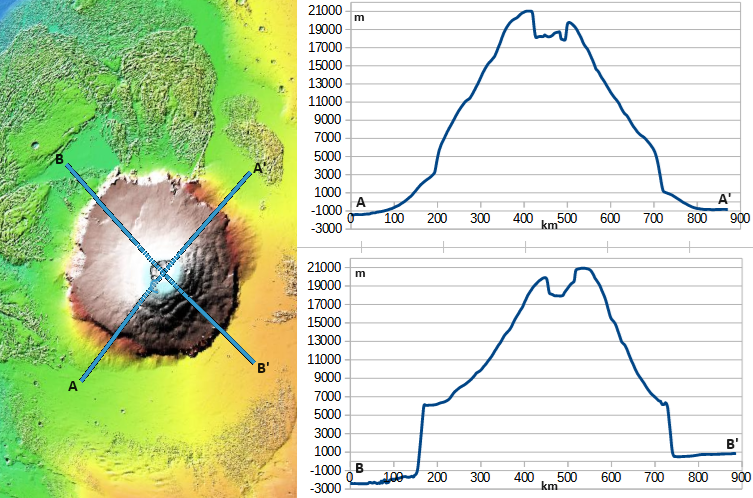
\includegraphics[width=.87\textwidth]{chapters/chp3_pics/Olympus_Mons_Elevation_Profiles.png}
\caption{\textit{Elevation profiles of Olympus Mons along SW-to-NE and NW-to-SE transects across the mountain. Image from Wikipedia}}
    \label{fig:olympus_mons}
\end{figure}




\subsubsection*{Level Curves} \index{Level Curves}

\noindent Level curves of a function \( f(x, y) \) are the set of points in the \( xy \)-plane where the function takes on a constant value \( k \), expressed by the equation \( f(x, y) = k \). By plotting these curves for various values of \( k \), we can visualize the function in two dimensions, gaining insights into its behavior without needing to represent the full three-dimensional surface. You may have even seen these types of plots on geographic plots. These are yet another tool that aid in understanding the shape of the terrain and identifying features like hills and valleys.

    \begin{figure}[H]
        \centering
\begin{tikzpicture}[scale=1.7,line cap=round,line join=round,
   x={(-0.7766cm,-0.1369cm)},y={(0.6300cm,-0.1688cm)},z={(0cm,0.9761cm)}]
\def\xmin{1}
\def\ymin{0.7}
\pgfmathsetmacro\xstep{\xmin-0.2}
\pgfmathsetmacro\ystep{\ymin-0.1}
\def\h{-1.4} % projection height
% blue lines, sections perpendicular to the x axis
\foreach\i in{-\xmin,-\xstep,...,\xmin}
{%                 domain in which z>=-1
  \pgfmathsetmacro\xdom{min(\ymin,sqrt(-0.5-\i*\i+0.5*sqrt(5+8*\i*\i)))}
  \draw[blue] plot[domain=-\xdom:\xdom,samples=25,smooth]
    (\i,\x,{-(\i*\i+\x*\x)*(\i*\i+\x*\x)+(\i*\i-\x*\x)});
}
% cyan lines, sections perpendicular to the y axis
\foreach\i in{-\ymin,-\ystep,...,\ymin}
{%                 domain in which z>=-1
  \pgfmathsetmacro\xdom{min(\xmin,sqrt(0.5-\i*\i+0.5*sqrt(5-8*\i*\i)))} 
  \draw[cyan] plot[domain=-\xdom:\xdom,samples=25,smooth]
    (\x,\i,{-(\x*\x+\i*\i)*(\x*\x+\i*\i)+(\x*\x-\i*\i)});
}
% Bernouilli's lemniscate (and projection)
\foreach\a in {0,180} \foreach\z in {0,\h}
{%
  \draw[thick,red] plot[domain=-45+\a: 45+\a,samples=25,smooth]
    ({sqrt(cos(2*\x))*cos(\x)},{sqrt(cos(2*\x))*sin(\x)},\z);
}
% Other level curves (and projections)
\def\z{0.2}
\pgfmathsetmacro\xdom{0.5*acos(2*sqrt(\z))-0.005} % precission problem, I think
\foreach\zz in {\z,\h} \foreach\a in {0,180} \foreach\s in {-1,1}
{%
  \draw[red] plot[domain=\a-\xdom:\a+\xdom,samples=25,smooth]
    ({sqrt(0.5*cos(2*\x)+0.5*\s*sqrt(cos(2*\x)*cos(2*\x)-4*\z))*cos(\x)},
     {sqrt(0.5*cos(2*\x)+0.5*\s*sqrt(cos(2*\x)*cos(2*\x)-4*\z))*sin(\x)},\zz);
}
\foreach\z in {-0.2,-0.4,-0.6} \foreach\zz in {\z,\h}
{%
  \draw[red] plot[domain=-180:180,samples=51,smooth]
   ({sqrt(0.5*cos(2*\x)+0.5*sqrt(cos(2*\x)*cos(2*\x)-4*\z))*cos(\x)},
    {sqrt(0.5*cos(2*\x)+0.5*sqrt(cos(2*\x)*cos(2*\x)-4*\z))*sin(\x)},\zz);
}
% axes
\draw[-latex] (0,0,0) -- (2,0,0) node[left]  {$x$};
\draw[-latex] (0,0,0) -- (0,2,0) node[right] {$y$};
\draw[-latex] (0,0,0) -- (0,0,1) node[above] {$z$};
\end{tikzpicture}
\caption{\textit{A 3D surface with its level curves projected below, including the Bernoulli lemniscate (the infinity shaped level curve)}}
\end{figure}


\noindent Now that we have a basic understanding of what level curves are and why they are useful, let's explore the process of plotting them in more detail. Level curves provide a two-dimensional representation of a function of two variables by showing all points \( (x, y) \) where the function takes on the same value \( k \). This visualization is particularly helpful for understanding the behavior of multivariable functions without requiring a full 3D plot. Here's how to systematically plot level curves step by step:

\begin{enumerate}
    \item \textbf{Select Values of \( k \):} Choose several constant values for \( k \) that capture the key features of the function. It's important to select a range of \( k \) values—both positive and negative, if applicable—to represent the function's full behavior. For functions with periodic or oscillatory behavior, ensure the \( k \)-values align with significant points such as peaks, troughs, and zeros.

    \item \textbf{Set \( f(x, y) = k \):} For each chosen value of \( k \), substitute it into the function \( f(x, y) \) to define the corresponding level curve. This equation represents all points \( (x, y) \) where the function equals \( k \).

    \item \textbf{Solve for One Variable in Terms of the Other:} Rearrange the equation \( f(x, y) = k \) to express \( y \) as a function of \( x \), or \( x \) as a function of \( y \), if possible. For example, in circular or radial symmetry, the equation might simplify to an expression for \( r^2 = x^2 + y^2 \). For more complex functions, this step may involve approximations or parametric forms.

    \item \textbf{Plot Each Level Curve:} Using the equations derived, carefully plot the curves on the \( xy \)-plane. For simple equations, this can be done by hand. For more intricate equations, consider using graphing tools or software to ensure accuracy. Ensure that each curve is plotted with sufficient points to capture its shape.

    \item \textbf{Label the Curves:} Clearly label each curve with its corresponding \( k \)-value. This can be done directly on the graph or through a legend. For enhanced clarity, consider using color coding to visually differentiate the curves based on their \( k \)-values.

    \item \textbf{Analyze the Overall Behavior:} Once the level curves are plotted, examine their spacing and patterns. For instance, closely spaced curves indicate regions of rapid change in the function, while widely spaced curves suggest more gradual variation. This step helps in interpreting the nature of the function and its gradients.
\end{enumerate}

\exampleline
\begin{example}
Consider the function \( z = \sin(x^2 + y^2) \) defined for all \( (x, y) \in \mathbb{R}^2 \).

\begin{enumerate}
    \item Plot the graph of \( z = \sin(x^2 + y^2) \) as a surface in 3D space.
    \item Plot the level curves of \( z = \sin(x^2 + y^2) \) for selected \( z \)-values computed by hand.
\end{enumerate}

\begin{solution}
\begin{enumerate}
    \item The graph of \( z = \sin(x^2 + y^2) \) exhibits circular symmetry. Recall that
    \[
    \begin{aligned}
    \sin(\theta) = 1 &\quad \text{if} \quad \theta = \frac{\pi}{2}+2\pi n,\\[6pt]
    \sin(\theta) = -1 &\quad \text{if} \quad \theta = -\frac{\pi}{2}+2\pi n,\\[6pt]
    \sin(\theta) = 0 &\quad \text{if} \quad \theta = \pi n,
    \end{aligned}
    \]
    for any integer \( n \). Since \( \theta = x^2+y^2 \), the peaks (\( z=1 \)) occur when
    \[
    x^2+y^2 = \frac{\pi}{2}+2\pi n,
    \]
    the troughs (\( z=-1 \)) when
    \[
    x^2+y^2 = -\frac{\pi}{2}+2\pi n,
    \]
    and the zeros (\( z=0 \)) when
    \[
    x^2+y^2 = \pi n.
    \]

    \begin{figure}[H]
        \centering
        \resizebox{0.55\textwidth}{!}{%
            \begin{tikzpicture}
                \begin{axis}[
                    view={45}{45},
                    xlabel={$x$}, ylabel={$y$}, zlabel={$z$},
                    colormap/cool,
                    grid=major,
                    domain=-2:2,
                    y domain=-2:2,
                    samples=30,
                    z buffer=sort
                ]
                \addplot3[surf] {sin(deg(x^2 + y^2))};
                \end{axis}
            \end{tikzpicture}
        }
        \caption{\textit{Graph of \( z = \sin(x^2+y^2) \), a sinusoidal surface.}}
        \label{fig:surface_sin_x2y2}
    \end{figure}

    \item To draw the level curves, we set \( \sin(x^2+y^2)=k \) for specific \( k \)-values. This gives:
    \begin{itemize}
        \item \textbf{For \( z=1 \):} Solve 
        \[
        x^2+y^2 = \frac{\pi}{2}+2\pi n \quad \Longrightarrow \quad r = \sqrt{\frac{\pi}{2}+2\pi n}.
        \]
        For example,
        \[
        \begin{aligned}
        n=0:\quad r &= \sqrt{\frac{\pi}{2}} \approx 1.25,\\[6pt]
        n=1:\quad r &= \sqrt{\frac{5\pi}{2}} \approx 2.80
        \end{aligned}
        \]
        
        \item \textbf{For \( z=-1 \):} Solve 
        \[
        x^2+y^2 = -\frac{\pi}{2}+2\pi n \quad (n \geq 1) \quad \Longrightarrow \quad r = \sqrt{-\frac{\pi}{2}+2\pi n}.
        \]
        For example,
        \[
        \begin{aligned}
        n=1:\quad r &= \sqrt{\frac{3\pi}{2}} \approx 2.17,\\[6pt]
        n=2:\quad r &= \sqrt{\frac{7\pi}{2}} \approx 3.32
        \end{aligned}
        \]
        
        \item \textbf{For \( z=0 \):} Solve 
        \[
        x^2+y^2 = \pi n \quad \Longrightarrow \quad r = \sqrt{\pi n}.
        \]
        For example,
        \[
        \begin{aligned}
        n=1:\quad r &= \sqrt{\pi} \approx 1.77,\\[6pt]
        n=2:\quad r &= \sqrt{2\pi} \approx 2.51
        \end{aligned}
        \]
    \end{itemize}

\begin{figure}[H]
    \centering
    \begin{tikzpicture}[scale=0.35]
        % Axes
        \draw[->] (-9,0) -- (9,0) node[anchor=north] {$x$};
        \draw[->] (0,-9) -- (0,9) node[anchor=west] {$y$};

        % Level curves for z=1 (blue)
        \draw[blue, thick] (0,0) circle (1.25);
        \draw[blue, thick] (0,0) circle (2.80);
        \draw[blue, thick] (0,0) circle (3.76);
        \draw[blue, thick] (0,0) circle (4.52);

        % Level curves for z=-1 (red)
        \draw[red, thick] (0,0) circle (2.17);
        \draw[red, thick] (0,0) circle (3.32);
        \draw[red, thick] (0,0) circle (4.16);
        \draw[red, thick] (0,0) circle (4.86);

        % Level curves for z=0 (green)
        \draw[green, thick] (0,0) circle (1.77);
        \draw[green, thick] (0,0) circle (2.51);
        \draw[green, thick] (0,0) circle (3.07);
        \draw[green, thick] (0,0) circle (3.54);

        % Legend
        \node[draw=none, fill=none, anchor=north west] at (10,6) {
            \begin{tikzpicture}
                \draw[blue, thick] (0,0) -- (1,0) node[anchor=west] {$z=1$};
                \draw[red, thick] (0,-0.5) -- (1,-0.5) node[anchor=west] {$z=-1$};
                \draw[green, thick] (0,-1) -- (1,-1) node[anchor=west] {$z=0$};
            \end{tikzpicture}
        };
    \end{tikzpicture}
    \caption{\textit{Level curves for \( z = \sin(x^2+y^2) \) with additional rings.}}
\end{figure}

\end{enumerate}
\end{solution}
\end{example}

\exampleline
\begin{example}
Consider the function \( z = \cos(y) \) defined for all \( (x, y) \in \mathbb{R}^2 \).

\begin{enumerate}
    \item Plot the graph of \( z = \cos(y) \) as a surface in 3D space.
    \item Plot the level curves of \( z = \cos(y) \) for selected \( z \)-values computed by hand.
\end{enumerate}

\begin{solution}
\begin{enumerate}
    \item The graph of \( z = \cos(y) \) represents a cosine wave in the \( y \)-direction that is extruded along the \( x \)-axis. As \( y \) varies, \( z \) oscillates between \(-1\) and \(1\).

    \begin{figure}[H]
        \centering
        \resizebox{0.55\textwidth}{!}{%
            \begin{tikzpicture}
                \begin{axis}[
                    view={45}{45},
                    xlabel={$x$}, ylabel={$y$}, zlabel={$z$},
                    colormap/cool,
                    grid=major,
                    domain=-3:3,
                    y domain=-6:6,
                    samples=30,
                    z buffer=sort
                ]
                \addplot3[surf] {cos(deg(y))};
                \end{axis}
            \end{tikzpicture}
        }
        \caption{\textit{Graph of \( z = \cos(y) \), a cosine wave surface extruded along \( x \).}}
        \label{fig:surface_cos_y}
    \end{figure}

    \item To find the level curves, we set \( \cos(y)=k \) for specific values of \( k \) (with \( -1 \le k \le 1 \)). The general solutions for \( y \) are:
    \[
    \begin{aligned}
    \cos(y) = 1 \quad &\Longrightarrow \quad y = 0 + 2\pi n,\\[6pt]
    \cos(y) = -1 \quad &\Longrightarrow \quad y = \pi + 2\pi n,\\[6pt]
    \cos(y) = 0 \quad &\Longrightarrow \quad y = \frac{\pi}{2} + \pi n,
    \end{aligned}
    \]
    where \( n \) is any integer. For a few specific level curves, we choose:
    \begin{itemize}
        \item \textbf{\( z=1 \):} \( y = 0,\, 2\pi,\, -2\pi,\, \ldots \)
        \item \textbf{\( z=-1 \):} \( y = \pi,\, -\pi,\, 3\pi,\, \ldots \)
        \item \textbf{\( z=0 \):} \( y = \frac{\pi}{2},\, -\frac{\pi}{2},\, \frac{3\pi}{2},\, \ldots \)
    \end{itemize}
    Since \( x \) is unrestricted, the level curves in the \( xy \)-plane are horizontal lines at these \( y \)-values.

    \begin{figure}[H]
        \centering
        \begin{tikzpicture}[scale=0.5]
            % Draw axes
            \draw[->] (-5,0) -- (5,0) node[anchor=north] {$x$};
            \draw[->] (0,-4) -- (0,4) node[anchor=east] {$y$};
            
            % Level curve for z=1 (blue): y = 0
            \draw[blue, thick] (-5,0) -- (5,0);
            
            % Level curves for z=-1 (red): y = π and y = -π
            \draw[red, thick] (-5,3.14) -- (5,3.14);
            \draw[red, thick] (-5,-3.14) -- (5,-3.14);
            
            % Level curves for z=0 (green): y = π/2 and y = -π/2
            \draw[green, thick] (-5,1.57) -- (5,1.57);
            \draw[green, thick] (-5,-1.57) -- (5,-1.57);
            
            % Legend
            \node[draw=none, fill=none, anchor=north west] at (6,3) {
                \begin{tikzpicture}[scale=0.8]
                    \draw[blue, thick] (0,0) -- (1,0) node[anchor=west] {$z=1$};
                    \draw[red, thick] (0,-0.5) -- (1,-0.5) node[anchor=west] {$z=-1$};
                    \draw[green, thick] (0,-1) -- (1,-1) node[anchor=west] {$z=0$};
                \end{tikzpicture}
            };
        \end{tikzpicture}
        \caption{\textit{Level curves for \( z = \cos(y) \) in the \( xy \)-plane.}}
    \end{figure}
\end{enumerate}
\end{solution}
\end{example}
\exampleline




\subsubsection*{Common 3D Equations}
\noindent As is the case in single-variable mathematics, we can depend on familiar examples to help make sense of functions on sight.

\begin{itemize}
    \item \textbf{Quadric Surfaces:} Paraboloids, hyperboloids, and ellipsoids are common surfaces that can often be graphed as functions of \( x \) and \( y \). These surfaces are studied in more detail in Lecture 1.5. Examples include:
    \begin{itemize}
        \item Paraboloid: \( z = x^2 + y^2 \)
        \item Hyperboloid of One Sheet: \( x^2 + y^2 - z^2 = 1 \)
        \item Ellipsoid: \( \frac{x^2}{a^2} + \frac{y^2}{b^2} + \frac{z^2}{c^2} = 1 \)
    \end{itemize}
    
    \item \textbf{Sphere:} A sphere represents a special case of an ellipsoid where all axes are equal. The equation is: 
    \[
    x^2 + y^2 + z^2 = r^2
    \]
    
    \item \textbf{Plane:} A plane can be described as a linear function in three variables. For example:
    \[
    z = ax + by + c
    \]
    
    \item \textbf{Cylinder:} Cylinders are surfaces generated by extending a curve along a straight line parallel to an axis. Examples include:
    \begin{itemize}
        \item Circular Cylinder: \( x^2 + y^2 = r^2 \)
        \item Parabolic Cylinder: \( z = x^2 \)
    \end{itemize}
    
    \item \textbf{Cone:} A cone is a surface that extends a curve in a way that all points of the curve are connected to a single vertex. For example:
    \[
    z^2 = x^2 + y^2
    \]
\end{itemize}

\subsection*{Functions of Three or More Variables} \index{Functions of Three or More Variables}

\noindent A function of three variables assigns a real number \( w = f(x, y, z) \) to each point \( (x, y, z) \) within a subset of \( \mathbb{R}^3 \). The challenge in working with such functions lies in the fact that their graphs exist in four-dimensional space, a realm beyond our ability to visualize directly. Unlike the graph of a function of one variable, which forms a curve in \( \mathbb{R}^2 \), or a function of two variables, which forms a surface in \( \mathbb{R}^3 \), the graph of \( f(x, y, z) \) resists geometric representation. Despite this limitation, a variety of powerful techniques enable us to analyze and understand these functions with clarity and precision. Specifically, the most comprehensive way that I can think about it is by the analogy of a three-dimensional shadow: a shadow reduces a 3D object down to 2D, therefore a 3D object is the shadow of a 4D object. This means that projections will be our greatest ally. \\

\noindent To streamline notation for functions of multiple variables, it is common to represent the input \( (x, y, z) \) as a single entity, often written as \( \mathbf{x} \). This allows us to express \( f(x, y, z) \) in a more concise form:
\[
f(\mathbf{x}),
\]
where \( \mathbf{x} \) represents the vector of input variables:
\[
\mathbf{x} = (x, y, z).
\]
This notation generalizes naturally to functions of \( n \) variables, where \( \mathbf{x} = (x_1, x_2, \ldots, x_n) \) is a vector in \( \mathbb{R}^n \). To emphasize the structure of the input variables, we can further represent \( \mathbf{x} \) as a column vector:
\[
\mathbf{x} = 
\begin{bmatrix}
x \\ 
y \\ 
z
\end{bmatrix}.
\]
With this notation, the function \( f(x, y, z) \) becomes \( f(\mathbf{x}) \), where \( \mathbf{x} \) is the input vector. Alternatively, we can express \( \mathbf{x} \) explicitly as a column vector:
\[
f(\mathbf{x}) = f\left(\begin{bmatrix} x \\ y \\ z \end{bmatrix}\right),
\]
providing a unified framework for analyzing functions of several variables. For instance, a temperature field \( T \) in three-dimensional space can be expressed as:
\[
T = f(\mathbf{t}) = f\left(\begin{bmatrix} t_x \\ t_y \\ t_z \end{bmatrix}\right) =  f(t_x,t_y,t_z) = t_x^2 + t_y^2 + t_z^2
\]
where \( \mathbf{t} \) represents a point in \( \mathbb{R}^3 \). This column vector-based notation is particularly valuable in advanced topics like gradients, divergence, and vector-valued functions, as it simplifies both expression and computation.




\subsubsection*{Graphs and Visualization}

\noindent While we cannot graph functions of three variables directly in three-dimensional space, we can understand them through level surfaces and projections. A \textbf{level surface} is the set of all points \((x, y, z)\) in the domain of \(f(x, y, z)\) where the function takes a constant value, \( w = k \). These surfaces are three-dimensional analogues of level curves for functions of two variables. For example, fixing \( w = 0 \), the level surface \( f(x, y, z) = 0 \) provides a snapshot of the function's behavior in three-dimensional space. \\

\noindent The idea is analogous to projections, where we imagine the three-dimensional representation of a function as the ``shadow" of its four-dimensional graph. By holding one variable constant, such as \( z = 0 \), we reduce the function to \( w = f(x, y, 0) \), which can be plotted as a surface in three-dimensional space. Repeating this process for various fixed values of \( z \) (or any other variable) gives a series of surfaces that collectively reveal the structure of the original function. This approach bridges the gap between our spatial intuition and the abstraction of higher-dimensional spaces.

\subsubsection*{Level Surfaces} \index{Level Surfaces}

\noindent Plotting a level surface will be very similar to our level curves. Let's take a look at a sphere \(f(x, y, z) = x^2 + y^2 + z^2\). The level surfaces are determined by solving:
\[
f(x, y, z) = k \implies x^2 + y^2 + z^2 = k.
\]

\noindent For different values of \( k \), the level surfaces represent spheres centered at the origin with radius \(\sqrt{k}\):
\begin{itemize}
    \item \( k = 1 \): Sphere of radius 1.
    \item \( k = 4 \): Sphere of radius 2.
    \item \( k = 9 \): Sphere of radius 3.
\end{itemize}

\noindent To visualize these level surfaces, we plot the spheres for \( k = 1, 4, 9 \). The surfaces demonstrate the isotropic nature of the function \( f(x, y, z) \), where the value of \( w \) depends only on the distance from the origin.

\begin{figure}[H]
    \centering
    \begin{tikzpicture}
        \begin{axis}[
            view={60}{30},
            axis equal image,
            hide axis,
            width=12cm,
            height=12cm,
            xmin=-4, xmax=4,
            ymin=-4, ymax=4,
            zmin=-4, zmax=4,
            clip=false, % Prevent clipping of callouts
        ]
            % Sphere of radius 1 (k=1)
            \addplot3[
                surf,
                shader=flat,
                opacity=0.3,
                samples=30,
                samples y=15,
                domain=0:360,
                y domain=0:180,
                z buffer=sort,
                fill=blue!50,
                draw=blue,
            ]
            ({1*cos(x)*sin(y)},
             {1*sin(x)*sin(y)},
             {1*cos(y)});
             
            % Sphere of radius 2 (k=4)
            \addplot3[
                surf,
                shader=flat,
                opacity=0.3,
                samples=30,
                samples y=15,
                domain=0:360,
                y domain=0:180,
                z buffer=sort,
                fill=green!50,
                draw=green,
            ]
            ({2*cos(x)*sin(y)},
             {2*sin(x)*sin(y)},
             {2*cos(y)});
             
            % Sphere of radius 3 (k=9)
            \addplot3[
                surf,
                shader=flat,
                opacity=0.3,
                samples=30,
                samples y=15,
                domain=0:360,
                y domain=0:180,
                z buffer=sort,
                fill=red!50,
                draw=red,
            ]
            ({3*cos(x)*sin(y)},
             {3*sin(x)*sin(y)},
             {3*cos(y)});
             
            % Callout for Sphere of radius 1 (k=1)
            \draw[->, thick, blue] (axis cs: -0.7, -0.7, -0.7) -- (axis cs: -1.2, -1.2, -1.2);
            \node[anchor=east, blue] at (axis cs: -1.3, -1.3, -1.3) {Sphere \( r = 1 \) ($k=1$)};
            
            % Callout for Sphere of radius 2 (k=4)
            \draw[->, thick, green!70!black] (axis cs: -1.4, -1.4, -1.4) -- (axis cs: -2.4, -2.4, -2.4);
            \node[anchor=east, green!70!black] at (axis cs: -2.5, -2.5, -2.5) {Sphere \( r = 2 \) ($k=4$)};
            
            % Callout for Sphere of radius 3 (k=9)
            \draw[->, thick, red] (axis cs: -2.1, -2.1, -2.1) -- (axis cs: -3.4, -3.4, -3.4);
            \node[anchor=east, red] at (axis cs: -3.5, -3.5, -3.5) {Sphere \( r = 3 \) ($k=9$)};
        \end{axis}
    \end{tikzpicture}
    \caption{\textit{Level surfaces of \( f(x, y, z) = x^2 + y^2 + z^2 = k\) for \( k = 1, 4, 9 \), represented as concentric spheres}}
    \label{fig:level_surfaces_example}
\end{figure}

\noindent While this doesn't exactly paint the complete picture, you may begin to see how hypergeometry works. Perhaps you have seen a hypercube represented before but not sure why it looks like it does. With level surfaces it may begin to make more sense:


\begin{figure}[H]
    \centering
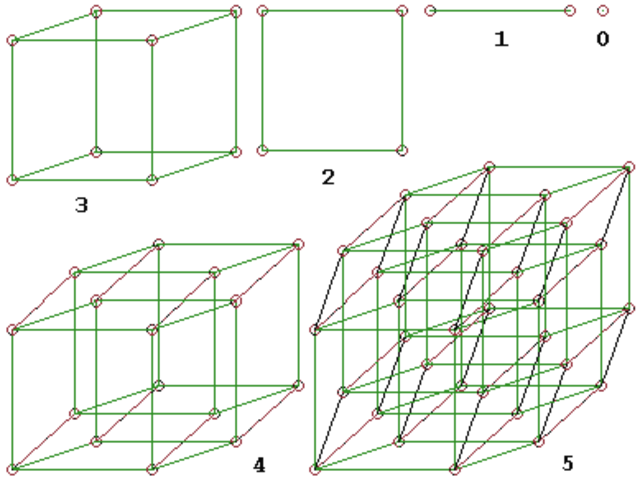
\includegraphics[width=.5\textwidth]{chapters/chp3_pics/hypercube.png}
\caption{\textit{Cubes of dimensions 1 through 5. Above three dimensions, these are often called hypercubes, or $n$-cubes. Image from Wikipedia}}
    \label{fig:4d_cube}
\end{figure}
%https://commons.wikimedia.org/wiki/File:WUERFEL5_0-_bis_5-dimensionale_Wuerfelanaloge.png
\subsection*{Visualizing Functions of Several Variables}

\noindent As the number of variables in a function increases, direct visualization becomes increasingly challenging. For functions of two or three variables, graphs and level sets provide intuitive insights. However, for functions involving more than three variables, such as \( f(x_1, x_2, \ldots, x_n) \), we rely on abstract representations, projections, and numerical tools to understand their behavior.

\paragraph{Higher-Dimensional Analogues:} In higher dimensions, familiar geometric objects like lines, planes, and spheres generalize:
\begin{itemize}
    \item A \textbf{hyperplane} in \( \mathbb{R}^n \) is defined by a linear equation, such as \( a_1x_1 + a_2x_2 + \cdots + a_nx_n = c \). It is the \( n \)-dimensional analogue of a plane in \( \mathbb{R}^3 \).
    \item A \textbf{hypersphere} in \( \mathbb{R}^n \) is defined by \( x_1^2 + x_2^2 + \cdots + x_n^2 = r^2 \). In \( \mathbb{R}^4 \), for example, this represents the set of points equidistant from a center, analogous to a sphere in \( \mathbb{R}^3 \).
\end{itemize}

\paragraph{Applications in Machine Learning:} \index{Machine Learning} Functions of several variables are fundamental in machine learning, particularly in classification tasks. For instance:
\begin{itemize}
    \item \textbf{Hyperplanes in Classification:} In supervised learning, hyperplanes are often used to separate data points belonging to different classes. For example, a linear classifier uses a hyperplane to divide the feature space into regions corresponding to different categories.
    \item \textbf{Support Vector Machines (SVMs):} SVMs are powerful classification algorithms that construct an optimal hyperplane to maximize the margin between data points of different classes. Mathematically, the hyperplane is defined as:
    \[
    \mathbf{w} \cdot \mathbf{x} - b = 0,
    \]
    where \( \mathbf{w} \) is the weight vector, \( \mathbf{x} \) is a data point, and \( b \) is a bias term. The margin is maximized by solving an optimization problem involving the constraint:
    \[
    y_i (\mathbf{w} \cdot \mathbf{x}_i - b) \geq 1,
    \]
    where \( y_i \) represents the class label of \( \mathbf{x}_i \).
\end{itemize}


\begin{figure}[H]
    \centering
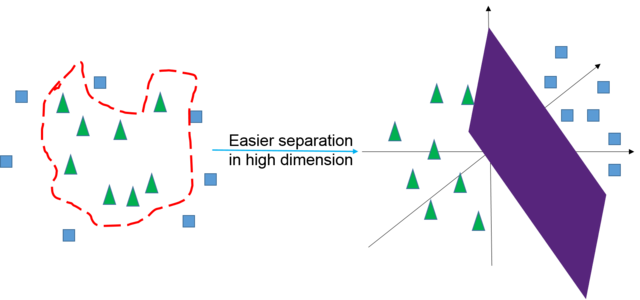
\includegraphics[width=.7\textwidth]{chapters/chp3_pics/Supporting_Vector_Machine.png}
\caption{\textit{Hyperplanes used for optimal classification in SVMs. Image from Wikipedia}}
    \label{fig:svm}
\end{figure}
%https://commons.wikimedia.org/wiki/File:Supporting_Vector_Machine.png

\noindent Although these applications arise in higher dimensions, the underlying concepts of hyperplanes and optimization are rooted in multivariable calculus.



\newpage


\lecture{Limits and Continuity} \index{Limits and Continuity}

\noindent In single-variable calculus, the concepts of limits and continuity form the foundation for understanding the behavior of functions near points of interest and for establishing the differentiability and integrability of functions. In multivariable calculus, these ideas extend naturally but require a more nuanced treatment due to the increased complexity introduced by multiple independent variables. This lecture delves into the concepts of limits and continuity in the context of multivariable functions, exploring their definitions, properties, and challenges.

\subsection*{Limits in Higher Dimensions}

\noindent The concept of a limit is a cornerstone of calculus and extends naturally to functions of several variables. However, understanding this extension requires a thoughtful approach, as the introduction of additional variables adds layers of complexity. \\ \\ In single-variable calculus, we define the limit \( \lim_{x \to a} f(x) = L \) as the value \( L \) that \( f(x) \) approaches as \( x \) gets arbitrarily close to \( a \). For multivariable functions, the same principle applies, but now the input \( (x, y) \) can approach a target point \( (a, b) \) from infinitely many directions in the plane. This distinction is key: in one dimension, there are only two possible approaches to \( a \) (from the left or right), whereas in two dimensions, there are infinitely many paths. 

\begin{figure}[H]
    \centering
\begin{tikzpicture}
\begin{axis}[
    view={60}{30},
    xlabel={$x$},
    ylabel={$y$},
    zlabel={$f(x, y)$},
    domain=-1:1,
    y domain=-1:1,
    samples=50,
    samples y=50,
    zmin=-1,
    zmax=1,
    colorbar,
    colormap/viridis,
]
\addplot3[surf] {x*y/(x^2 + y^2)};
\end{axis}
\end{tikzpicture}
    \caption{\textit{Graph of \(z = \frac{x y}{x^2 + y^2} \), where the limit does not exist at $(0,0)$}}
    \label{fig:surface_xy_over_x2y2}
\end{figure}


\noindent To understand limits intuitively, imagine the behavior of a function \( f(x, y) \) as you move closer and closer to a fixed point \( (a, b) \). The value of \( f(x, y) \) should stabilize and become arbitrarily close to a specific number \( L \), regardless of the path taken. If the value of \( f(x, y) \) changes depending on the path, the limit does not exist.

\subsubsection*{Properties of Multivariable Limits} \index{Multivariable Limits}

\noindent Before diving into techniques for evaluating limits, it is helpful to understand some basic properties that govern multivariable limits. These properties, analogous to their single-variable counterparts, provide useful shortcuts and insights into the behavior of multivariable functions as they approach a limit.

\begin{itemize}
    \item \textbf{Linearity:} If \( \lim_{(x, y) \to (a, b)} f(x, y) = L \) and \( \lim_{(x, y) \to (a, b)} g(x, y) = M \), then for any constants \( c_1 \) and \( c_2 \):
    \[
    \lim_{(x, y) \to (a, b)} \left[ c_1 f(x, y) + c_2 g(x, y) \right] = c_1 L + c_2 M.
    \]

    \item \textbf{Product Rule:} If \( \lim_{(x, y) \to (a, b)} f(x, y) = L \) and \( \lim_{(x, y) \to (a, b)} g(x, y) = M \), then:
    \[
    \lim_{(x, y) \to (a, b)} \left[ f(x, y) g(x, y) \right] = L \cdot M.
    \]

    \item \textbf{Quotient Rule:} If \( \lim_{(x, y) \to (a, b)} f(x, y) = L \) and \( \lim_{(x, y) \to (a, b)} g(x, y) = M \), with \( M \neq 0 \), then:
    \[
    \lim_{(x, y) \to (a, b)} \frac{f(x, y)}{g(x, y)} = \frac{L}{M}.
    \]

    \item \textbf{Composition Rule:} If \( \lim_{(x, y) \to (a, b)} f(x, y) = L \) and \( \lim_{z \to L} g(z) = N \), where \( g \) is continuous at \( L \), then:
    \[
    \lim_{(x, y) \to (a, b)} g(f(x, y)) = g(L).
    \]

    \item \textbf{Limits of Polynomials and Rational Functions:} For polynomial functions \( f(x, y) \) and \( g(x, y) \), the limit as \( (x, y) \to (a, b) \) can often be found by direct substitution:
    \[
    \lim_{(x, y) \to (a, b)} f(x, y) = f(a, b).
    \]
    For rational functions \( f(x, y)/g(x, y) \), this holds as long as \( g(a, b) \neq 0 \).

    \item \textbf{Continuity and Limits:} If \( f(x, y) \) is continuous at \( (a, b) \), then the limit as \( (x, y) \to (a, b) \) is simply the value of the function at that point:
    \[
    \lim_{(x, y) \to (a, b)} f(x, y) = f(a, b).
    \]
\end{itemize}

\noindent These properties simplify the evaluation of many limits and help identify when more advanced techniques, such as polar coordinates or path dependence analysis, may be necessary. Combined with the techniques described in the following section, they form the backbone of solving multivariable limit problems.

\subsubsection*{Basic Techniques for Evaluating Limits}

\noindent While the formal definition of a limit provides a rigorous foundation, solving limits in practice often relies on algebraic manipulation and analytical techniques familiar from single-variable calculus. These techniques aim to simplify the function or identify patterns that reveal the behavior of \( f(x, y) \) (or \( f(x, y, z) \), etc.) as the input approaches a specific point. Below are common methods used for evaluating multivariable limits:

\begin{itemize}
    \item \textbf{Substitution:} If the function is continuous at the point of interest, substitution is the simplest and most direct method. For example, to evaluate \( \lim_{(x, y) \to (a, b)} f(x, y) \), substitute \( x = a \) and \( y = b \) into \( f(x, y) \). If the resulting expression is well-defined, the limit is equal to the function's value at that point.

    \item \textbf{Factoring and Simplification:} Similar to single-variable calculus, factoring can help simplify expressions and eliminate terms causing indeterminate forms. For example, for functions like \( \frac{x^2 - y^2}{x - y} \), factoring the numerator reveals simplifications.

    \item \textbf{Rationalizing Using Conjugates:} For functions involving square roots, multiplying by the conjugate can simplify the expression and resolve indeterminate forms. For example:
    \[
    \lim_{(x, y) \to (0, 0)} \frac{\sqrt{x^2 + y^2} - 1}{x^2 + y^2}
    \]
    can be simplified by multiplying numerator and denominator by \( \sqrt{x^2 + y^2} + 1 \).

    \item \textbf{Path Dependence Analysis:} To determine whether a limit exists, evaluate the function along different paths approaching the same point. Common paths include:
    \begin{itemize}
        \item Horizontal or vertical lines, such as \( y = 0 \) or \( x = 0 \).
        \item Diagonal lines, such as \( y = mx \), where \( m \) is a constant slope.
        \item Curved paths, such as \( y = x^2 \) or \( y = \sin(x) \).
    \end{itemize}
    If the limit depends on the chosen path, the overall limit does not exist.

\noindent \textbf{Important:} Showing that the limit is the same along all straight-line paths \( y = mx \) is \textit{not} sufficient to prove a limit exists. One must also check nonlinear paths such as \( y = x^2 \). A classic example is \( f(x,y) = \frac{x^2 y}{x^4 + y^2} \), where the limit along every line through the origin is 0, but the limit along \( y = x^2 \) is \( \frac{1}{2} \).\\ \\

    \item \textbf{Polar Coordinates:} For limits approaching the origin in two dimensions, converting to polar coordinates can simplify expressions. Substituting \( x = r\cos\theta \) and \( y = r\sin\theta \) reduces a multivariable problem to a single variable \( r \), where \( r \to 0 \). For example:
    \[
    \lim_{(x, y) \to (0, 0)} \frac{x^2 + y^2}{x^2 - y^2}
    \]
    becomes:
    \[
    \lim_{r \to 0} \frac{r^2}{r^2(\cos^2\theta - \sin^2\theta)}.
    \]
\end{itemize}

\noindent These techniques provide a powerful toolkit for solving a wide variety of multivariable limit problems. While some methods, such as path analysis and polar coordinates, are specific to functions of multiple variables, others are naturally inherited from single-variable calculus. Keep in mind, not only can we take limits from $(x,y) \to (a,b)$, but $(x,y,z) \to (a,b,c)$ and higher dimensions. Let's now work some of these out.


\exampleline
\begin{example}
Evaluate the following limits:
\begin{enumerate}
    \item \( \lim_{(x, y) \to (0, 0)} x^2 + y^2 \)
    \item \( \lim_{(x, y) \to (1, 1)} \frac{\sqrt{x} - \sqrt{y}}{x - y} \)
    \item \( \lim_{(x, y, z) \to (0, 0, 0)} \frac{\sin(x^2 + y^2 + z^2)}{x^2 + y^2 + z^2} \)
    \item \( \lim_{(x, y) \to (0, 0)} \frac{x^2 - y^2}{x^2 + y^2} \)
\end{enumerate}

\begin{solution}
\begin{enumerate}
    \item For \( \lim_{(x, y) \to (0, 0)} x^2 + y^2 \):
    \begin{itemize}
        \item \textbf{Direct Substitution:} Since \( x^2 + y^2 \) is continuous, directly substituting \( (x, y) = (0, 0) \) gives:
        \[
        \lim_{(x, y) \to (0, 0)} x^2 + y^2 = 0^2 + 0^2 = 0.
        \]
    \end{itemize}

    \item For \( \lim_{(x, y) \to (1, 1)} \frac{\sqrt{x} - \sqrt{y}}{x - y} \):
    \begin{itemize}
        \item \textbf{Multiply by the Conjugate:} To simplify, multiply numerator and denominator by \( \sqrt{x} + \sqrt{y} \):
        \[
        \frac{\sqrt{x} - \sqrt{y}}{x - y} \cdot \frac{\sqrt{x} + \sqrt{y}}{\sqrt{x} + \sqrt{y}} = \frac{(\sqrt{x} - \sqrt{y})(\sqrt{x} + \sqrt{y})}{(x - y)(\sqrt{x} + \sqrt{y})} = \frac{x - y}{(x - y)(\sqrt{x} + \sqrt{y})}.
        \]
        Simplifying, we find:
        \[
        \frac{1}{\sqrt{x} + \sqrt{y}}.
        \]
        Substituting \( (x, y) = (1, 1) \):
        \[
        \lim_{(x, y) \to (1, 1)} \frac{\sqrt{x} - \sqrt{y}}{x - y} = \frac{1}{\sqrt{1} + \sqrt{1}} = \frac{1}{2}.
        \]
    \end{itemize}

    \item For \( \lim_{(x, y, z) \to (0, 0, 0)} \frac{\sin(x^2 + y^2 + z^2)}{x^2 + y^2 + z^2} \):
    \begin{itemize}
        \item \textbf{Convert to Spherical Coordinates:} Let \( r^2 = x^2 + y^2 + z^2 \), where \( r \to 0 \) as \( (x, y, z) \to (0, 0, 0) \). The expression becomes:
        \[
        \frac{\sin(x^2 + y^2 + z^2)}{x^2 + y^2 + z^2} = \frac{\sin(r^2)}{r^2}.
        \]
        Using the substitution \( u = r^2 \), where \( u \to 0^+ \) as \( r \to 0^+ \), the limit simplifies to:
        \[
        \lim_{u \to 0^+} \frac{\sin(u)}{u}.
        \]
        From single-variable calculus, it is known that:
        \[
        \lim_{u \to 0} \frac{\sin(u)}{u} = 1.
        \]
        Thus:
        \[
        \lim_{(x, y, z) \to (0, 0, 0)} \frac{\sin(x^2 + y^2 + z^2)}{x^2 + y^2 + z^2} = 1.
        \]
    \end{itemize}

    \item For \( \lim_{(x, y) \to (0, 0)} \frac{x^2 - y^2}{x^2 + y^2} \):
    \begin{itemize}
        \item \textbf{Path Dependence:} The value of the limit depends on the path taken to approach \( (0, 0) \).
        \begin{enumerate}
            \item \textbf{Path 1: \( y = 0 \):} Substituting \( y = 0 \) into the function:
            \[
            \frac{x^2 - y^2}{x^2 + y^2} = \frac{x^2 - 0^2}{x^2 + 0^2} = \frac{x^2}{x^2} = 1.
            \]
            \item \textbf{Path 2: \( x = 0 \):} Substituting \( x = 0 \) into the function:
            \[
            \frac{x^2 - y^2}{x^2 + y^2} = \frac{0^2 - y^2}{0^2 + y^2} = \frac{-y^2}{y^2} = -1.
            \]
            \item \textbf{Path 3: \( y = mx \):} Substituting \( y = mx \) into the function:
            \[
            \frac{x^2 - (mx)^2}{x^2 + (mx)^2} = \frac{x^2 - m^2x^2}{x^2 + m^2x^2}.
            \]
            Simplify:
            \[
            \frac{1 - m^2}{1 + m^2}.
            \]
        \end{enumerate}
        Since the limits differ based on the path taken:
        \[
        \text{The limit does not exist.}
        \]
    \end{itemize}
\end{enumerate}
\end{solution}
\end{example}
\exampleline

\subsubsection*{Other Techniques}
Beyond our core toolkit for evaluating multivariable limits, we can extend several powerful techniques from single-variable calculus into multiple dimensions. These methods often allow us to reduce complex multivariable problems into more manageable pieces that connect to our existing understanding. \\

\noindent The Squeeze Theorem extends naturally to multivariable functions, providing a powerful tool when direct evaluation proves difficult. If we can find two functions that ``squeeze" our target function and share the same limit, then our target function must approach that limit as well. Formally, if for all points $(x,y)$ in some neighborhood of $(a,b)$:
\[
g(x, y) \leq f(x, y) \leq h(x, y)
\]
and we have
\[
\lim_{(x, y) \to (a, b)} g(x, y) = \lim_{(x, y) \to (a, b)} h(x, y) = L,
\]
then we can conclude
\[
\lim_{(x, y) \to (a, b)} f(x, y) = L.
\]

\noindent To understand this intuitively, imagine the graphs of $g(x,y)$ and $h(x,y)$ forming a ``corridor" in three-dimensional space that contains the graph of $f(x,y)$. As we approach the point $(a,b)$, this corridor narrows to a single point with height $L$, forcing our function $f(x,y)$ to approach the same value. \\

\noindent When encountering indeterminate forms like $\frac{0}{0}$, we can apply reasoning similar to L'Hôpital's Rule by treating one variable as constant and analyzing the limit with respect to the other variable. While we haven't yet developed the machinery of partial derivatives, we can still analyze these limits by considering one variable at a time. For instance, when approaching a point $(a,b)$, we might:
\begin{itemize}
    \item First analyze $f(x,b)$ as $x \to a$, treating $y$ as the constant $b$
    \item Then analyze $f(a,y)$ as $y \to b$, treating $x$ as the constant $a$
    \item Compare these single-variable limits
\end{itemize}

\noindent For a function exhibiting an indeterminate form $\frac{0}{0}$, we can write:
\[
\lim_{x \to a} \frac{f(x,b)}{g(x,b)} = \lim_{x \to a} \frac{f'(x,b)}{g'(x,b)}
\]
where the derivatives are taken with respect to $x$ while treating $y$ as the constant $b$. However, we must exercise caution: equality of these single-variable limits is necessary but not sufficient for the existence of the multivariable limit. The multivariable nature of the functions introduces subtleties not present in single-variable calculus, particularly the need to verify that the limit is independent of the path taken to $(a,b)$. \\

\noindent These advanced techniques complement our earlier methods, often providing elegant solutions to complex limit problems that might otherwise prove intractable. Their application requires careful attention to the underlying assumptions and verification of path independence, but they significantly expand our ability to analyze multivariable limits.


\exampleline
\begin{example}
Evaluate the following limits using the advanced techniques we've just learned:
\begin{enumerate}
    \item \( \lim_{(x, y) \to (0, 0)} \frac{x^2y}{x^2 + y^2} \)
    \item \( \lim_{(x, y) \to (0, 0)} xy\sin\left(\frac{1}{x^2 + y^2}\right) \)
    \item \( \lim_{(x,y) \to (0,2)} \frac{e^{xy}-1}{x} \)
    \item \( \lim_{(x,y) \to (3,0)} \frac{\sqrt{x+y}-\sqrt{x}}{y} \)
\end{enumerate}

\begin{solution}
\begin{enumerate}
    \item For \( \lim_{(x, y) \to (0, 0)} \frac{x^2y}{x^2 + y^2} \):
    \begin{itemize}
        \item \textbf{Using the Squeeze Theorem:} Let's find bounds for this function.
        First, note that:
        \[
        \left|\frac{x^2y}{x^2 + y^2}\right| = |y| \cdot \left|\frac{x^2}{x^2 + y^2}\right|
        \]
        Since \( \frac{x^2}{x^2 + y^2} \leq 1 \) for all \( (x, y) \neq (0, 0) \), we have:
        \[
        \left|\frac{x^2y}{x^2 + y^2}\right| \leq |y|
        \]
        Therefore:
        \[
        -|y| \leq \frac{x^2y}{x^2 + y^2} \leq |y|
        \]
        As \( (x, y) \to (0, 0) \), we know \( |y| \to 0 \). By the Squeeze Theorem:
        \[
        \lim_{(x, y) \to (0, 0)} \frac{x^2y}{x^2 + y^2} = 0
        \]
    \end{itemize}

    \item For \( \lim_{(x, y) \to (0, 0)} xy\sin\left(\frac{1}{x^2 + y^2}\right) \):
    \begin{itemize}
        \item \textbf{Using the Squeeze Theorem:} First, recall that \( |\sin(z)| \leq 1 \) for all \( z \).
        Therefore:
        \[
        \left|xy\sin\left(\frac{1}{x^2 + y^2}\right)\right| \leq |xy|
        \]
        Now we need to show that \( |xy| \to 0 \) as \( (x, y) \to (0, 0) \).
        
        Let's use polar coordinates: \( x = r\cos\theta \), \( y = r\sin\theta \)
        Then:
        \[
        |xy| = |r\cos\theta \cdot r\sin\theta| = r^2|\cos\theta\sin\theta| \leq \frac{r^2}{2}
        \]
        Therefore:
        \[
        -\frac{r^2}{2} \leq xy\sin\left(\frac{1}{x^2 + y^2}\right) \leq \frac{r^2}{2}
        \]
        As \( (x, y) \to (0, 0) \), \( r \to 0 \), so by the Squeeze Theorem:
        \[
        \lim_{(x, y) \to (0, 0)} xy\sin\left(\frac{1}{x^2 + y^2}\right) = 0
        \]
        Note: Even though \( \frac{1}{x^2 + y^2} \) becomes unbounded as \( (x, y) \to (0, 0) \), the bounded nature of sine combined with the factor \( xy \) controls the overall behavior of the function.
    \end{itemize}

    \item For \( \displaystyle \lim_{(x,y) \to (0,2)} \frac{e^{xy}-1}{x} \):
    \begin{itemize}
        \item \textbf{Fixing \(y=2\) and applying L'Hôpital's Rule:} As \(y \to 2\), we treat the limit as a function of \(x\):
        \[
        \lim_{x\to 0} \frac{e^{2x}-1}{x}.
        \]
        This is a \( \frac{0}{0} \) indeterminate form. Differentiating with respect to \(x\) (with \(y\) held constant):
        \[
        \frac{d}{dx}\bigl(e^{2x}-1\bigr)=2e^{2x}, \quad \frac{d}{dx}(x)=1.
        \]
        Therefore, the limit becomes:
        \[
        \lim_{x\to 0} 2e^{2x} = 2e^0 = 2.
        \]
    \end{itemize}

    \item For \( \displaystyle \lim_{(x,y) \to (3,0)} \frac{\sqrt{x+y}-\sqrt{x}}{y} \):
    \begin{itemize}
        \item \textbf{Fixing \(x=3\) and applying L'Hôpital's Rule:} As \(x \to 3\), consider the limit as a function of \(y\):
        \[
        \lim_{y\to 0} \frac{\sqrt{3+y}-\sqrt{3}}{y}.
        \]
        This gives a \( \frac{0}{0} \) indeterminate form. Differentiating with respect to \(y\):
        \[
        \frac{d}{dy}\bigl(\sqrt{3+y}\bigr)=\frac{1}{2\sqrt{3+y}}, \quad \frac{d}{dy}(y)=1.
        \]
        Hence, the limit simplifies to:
        \[
        \lim_{y\to 0} \frac{1}{2\sqrt{3+y}} = \frac{1}{2\sqrt{3}}.
        \]
    \end{itemize}
\end{enumerate}
\end{solution}
\end{example}
\exampleline


\subsection*{Formal Definition}
To rigorously define the limit, we need a precise way to measure ``closeness" for points in two dimensions. Luckily, from Chapter 1 we know how to do this now. In the \( \mathbb{R}^2 \) plane, the distance between two points \( (x, y) \) and \( (a, b) \) is given by the Euclidean distance formula:
\[
\sqrt{(x-a)^2 + (y-b)^2}.
\]
We say that \( \lim_{(x, y) \to (a, b)} f(x, y) = L \) if we can make the value of \( f(x, y) \) arbitrarily close to \( L \) (within an error margin of \( \epsilon \)) by ensuring that \( (x, y) \) is sufficiently close to \( (a, b) \) (within a distance of \( \delta \)). \\ \\
The formal definition is expressed as follows:
\[
\lim_{(x, y) \to (a, b)} f(x, y) = L
\]
means that for every \( \epsilon > 0 \), there exists a \( \delta > 0 \) such that:
\[
0 < \sqrt{(x-a)^2 + (y-b)^2} < \delta \implies |f(x, y) - L| < \epsilon.
\]
Here’s what this means step by step:
\begin{itemize}
    \item \( \epsilon \) (epsilon): A small positive number that represents how close \( f(x, y) \) must be to \( L \). Think of this as the allowable error in the output of the function.
    \item \( \delta \) (delta): A small positive number that represents how close \( (x, y) \) must be to \( (a, b) \). This defines a circular region (a disk) around \( (a, b) \) with radius \( \delta \).
    \item The condition \( 0 < \sqrt{(x-a)^2 + (y-b)^2} < \delta \) ensures that \( (x, y) \) is close to \( (a, b) \) but not exactly at \( (a, b) \), as the limit depends on the behavior of the function near \( (a, b) \), not at \( (a, b) \) itself.
    \item The implication \( |f(x, y) - L| < \epsilon \) ensures that the function value is within \( \epsilon \) of \( L \) whenever \( (x, y) \) is within \( \delta \) of \( (a, b) \).
\end{itemize}

\noindent To visualize this concept, imagine a mountain with a peak at \( (a, b, L) \). As you climb the mountain from different starting points, you must arrive at the same height \( L \) to conclude that the peak has a well-defined elevation. If different paths lead to different heights, the notion of a single ``peak height" breaks down, and the limit does not exist. 

\begin{figure}[H]
    \centering
\begin{tikzpicture}
  \begin{axis}[
      view={60}{30}, % Adjust the viewing angle
      xlabel={$x$}, ylabel={$y$}, zlabel={$z$},
      axis lines=middle,
      xmin=-2, xmax=4,
      ymin=-2, ymax=4,
      zmin=-2, zmax=6,
      grid=major,
      ticks=none,
      scale=1.5, % Scales the geometries (axes, lines, surfaces)
      label style={font=\normalsize}, % Keeps label sizes the same
      tick label style={font=\small}, % Keeps tick labels consistent
  ]
      % Delta circle in the x-y plane
      \addplot3[samples=50,domain=0:360,thick,blue]
        ({2 - 0.5*cos(x)},{2 - 0.5*sin(x)},{0});
      
      % Dot at (a, b) in the x-y plane
      \addplot3[only marks, mark=*, mark options={red}, thick] coordinates {(2,2,0)};
      
      % Callout to (a, b)
      \draw[->,thick] (axis cs:2.5,2.5,0) -- (axis cs:2,2,0);
      \node[above right] at (axis cs:3.5,2,0) {$(a, b)$};
      
      % Callout to delta (radius size)
      \draw[->,thick] (axis cs:1,1.7,0) -- (axis cs:1.646,2.353,0);
      \node[below left] at (axis cs:0.3,2,0) {$\delta$};
      
      % Transparent surface above the x-y plane
      \addplot3[surf,opacity=0.4,samples=30,samples y=30,domain=0:4,y domain=0:4]
        {5 - 0.1*(x^2 + y^2)};
      
      % Dot at (a, b) on the surface
      \addplot3[only marks, mark=*, mark options={red}, thick] coordinates {(2,2,{5 - 0.1*(2^2 + 2^2)})};
      
      % Movable label for f(a,b)
      \node at (axis cs:2.8,2.8,{5 - 0.1*(2^2 + 2^2) + 0.2}) {$f(a,b)$};
      
      % Circle on the surface
      \addplot3[samples=50,domain=0:360,thick,blue]
        ({2 - 0.5*cos(x)},{2 - 0.5*sin(x)},{5 - 0.1*((2 - 0.5*cos(x))^2 + (2 - 0.5*sin(x))^2)});
      
      % Maximum height point on the circle on the surface
      \addplot3[only marks, mark=*, mark options={blue}, thick] 
        coordinates {(1.646, 1.646, 4.458)};
      
      % Minimum height point on the circle on the surface
      \addplot3[only marks, mark=*, mark options={blue}, thick] 
        coordinates {(2.354, 2.354, 3.892)};
      
      % Blue dot for L + epsilon on z-axis
      \addplot3[only marks, mark=*, mark options={blue}, thick] coordinates {(0, 0, 4.458)};
      \node[left] at (axis cs:-0.5, 0, 5.1) {$L + \epsilon$};

      % Blue dot for L - epsilon on z-axis
      \addplot3[only marks, mark=*, mark options={blue}, thick] coordinates {(0, 0, 3.892)};
      \node[left] at (axis cs:-0.5, 0, 3.1) {$L - \epsilon$};
      
      % Red dot for L on z-axis
      \addplot3[only marks, mark=*, mark options={red}, thick] coordinates {(0, 0, {5 - 0.1*(2^2 + 2^2)})};
      \node[left] at (axis cs:-0.5, 0, {5 - 0.1*(2^2 + 2^2)}) {$L$};
      
      % Dotted line from L + epsilon to maximum height on the surface
      \draw[dotted, thick] (axis cs:0,0,4.458) -- (axis cs:1.646,1.646,4.458);
      
      % Dotted line from L to f(a,b) on the surface
      \draw[dotted, thick] (axis cs:0,0,{5 - 0.1*(2^2 + 2^2)}) -- (axis cs:2,2,{5 - 0.1*(2^2 + 2^2)});
      
      % Dotted line from L - epsilon to minimum height on the surface
      \draw[dotted, thick] (axis cs:0,0,3.892) -- (axis cs:2.354,2.354,3.892);
  \end{axis}
\end{tikzpicture}
    \caption{\textit{Visualization of the \(\varepsilon\)-\(\delta\) definition for a function of two variables. The blue circle of radius \(\delta\) in the \(xy\)-plane surrounds \((a,b)\). The surface \(z = f(x,y)\) is shown with the corresponding curve on the surface above the \(\delta\)-circle. The values \(L + \varepsilon\) and \(L - \varepsilon\) on the \(z\)-axis mark the acceptable output range: the definition requires that whenever \((x,y)\) lies within the \(\delta\)-circle, the surface height stays between \(L - \varepsilon\) and \(L + \varepsilon\).}}
\end{figure}



\noindent The concept of limits extends to functions of three or more variables. For a function \( f(x, y, z) \), the limit as \( (x, y, z) \to (a, b, c) \) is defined similarly:
\[
\lim_{(x, y, z) \to (a, b, c)} f(x, y, z) = L
\]
if for every \( \epsilon > 0 \), there exists a \( \delta > 0 \) such that:
\[
0 < \sqrt{(x-a)^2 + (y-b)^2 + (z-c)^2} < \delta \implies |f(x, y, z) - L| < \epsilon.
\]
The principles remain the same, but the added dimension increases the complexity of path dependence and visualization. Tools like polar, cylindrical, or spherical coordinates are often used to simplify calculations. \\

\noindent This idea generalizes further to functions of \( n \)-variables, \( f(x_1, x_2, \dots, x_n) \). The limit as \( (x_1, x_2, \dots, x_n) \to (a_1, a_2, \dots, a_n) \) is defined as:
\[
\lim_{(x_1, x_2, \dots, x_n) \to (a_1, a_2, \dots, a_n)} f(x_1, x_2, \dots, x_n) = L
\]
if for every \( \epsilon > 0 \), there exists a \( \delta > 0 \) such that:
\[
0 < \sqrt{\sum_{i=1}^n (x_i - a_i)^2} < \delta \implies |f(x_1, x_2, \dots, x_n) - L| < \epsilon.
\]
Here, the distance metric generalizes to the Euclidean norm in \( n \)-dimensional space:
\[
\sqrt{\sum_{i=1}^n (x_i - a_i)^2},
\]
which measures the distance between the point \( (x_1, x_2, \dots, x_n) \) and the target \( (a_1, a_2, \dots, a_n) \). The \(\epsilon\)-\(\delta\) framework ensures that as \( (x_1, x_2, \dots, x_n) \) approaches \( (a_1, a_2, \dots, a_n) \) in this generalized space, the function value \( f(x_1, x_2, \dots, x_n) \) approaches \( L \), independent of the path taken. \\
\noindent Alternatively, the concept of limits can be compactly expressed using vector notation. For a function \( f(\mathbf{x}) \) where \( \mathbf{x} = (x_1, x_2, \dots, x_n) \) and the target point is \( \mathbf{a} = (a_1, a_2, \dots, a_n) \), the limit is written as:
\[
\lim_{\mathbf{x} \to \mathbf{a}} f(\mathbf{x}) = L,
\]
if for every \( \epsilon > 0 \), there exists a \( \delta > 0 \) such that:
\[
0 < \|\mathbf{x} - \mathbf{a}\| < \delta \implies |f(\mathbf{x}) - L| < \epsilon.
\]

\exampleline
\begin{example}
Using the formal definition of limits for multivariable functions, prove that:
\[
\lim_{(x, y) \to (0, 0)} x y = 0.
\]


\begin{solution}
To prove that:
\[
\lim_{(x, y) \to (0, 0)} x y = 0,
\]
we need to show that for every \( \epsilon > 0 \), there exists a \( \delta > 0 \) such that whenever \( 0 < \sqrt{(x - 0)^2 + (y - 0)^2} < \delta \), it follows that:
\[
|x y - 0| < \epsilon.
\]

\noindent \textbf{Proof:} Let \( \epsilon > 0 \) be given. We aim to find \( \delta > 0 \) such that if \( 0 < \sqrt{x^2 + y^2} < \delta \), then \( |x y| < \epsilon \). Note that since \( |x| \leq \sqrt{x^2 + y^2} \) and \( |y| \leq \sqrt{x^2 + y^2} \), we have:
\[
|x y| = |x||y| \leq \left( \sqrt{x^2 + y^2} \right) \left( \sqrt{x^2 + y^2} \right) = \left( \sqrt{x^2 + y^2} \right)^2.
\]

\noindent Now, choose \( \delta = \sqrt{\epsilon} \). Then \( \delta > 0 \) because \( \epsilon > 0 \). Suppose \( 0 < \sqrt{x^2 + y^2} < \delta \). Then:
\[
|x y| \leq \left( \sqrt{x^2 + y^2} \right)^2 < \delta^2 = (\sqrt{\epsilon})^2 = \epsilon.
\]

\noindent  Therefore, whenever \( 0 < \sqrt{x^2 + y^2} < \delta \), it follows that \( |x y| < \epsilon \). \\

\noindent  \textbf{Conclusion:} For every \( \epsilon > 0 \), we have found \( \delta = \sqrt{\epsilon} > 0 \) such that:
\[
0 < \sqrt{x^2 + y^2} < \delta \implies |x y - 0| < \epsilon.
\]
\noindent  Hence, by the formal definition of limits for multivariable functions,
\[
\lim_{(x, y) \to (0, 0)} x y = 0.
\]
\end{solution}
\end{example}
\exampleline


\subsection*{Continuity in Multivariable Functions} \index{Continuous Functions}

\noindent Continuity is a fundamental concept in calculus, naturally extending from single-variable functions to multivariable functions. Intuitively, a function \( f(x, y) \) is continuous at a point \( (a, b) \) if small changes in \( (x, y) \) near \( (a, b) \) result in small changes in \( f(x, y) \). Formally, \( f(x, y) \) is continuous at \( (a, b) \) if:
\[
\lim_{(x, y) \to (a, b)} f(x, y) = f(a, b).
\]
This definition implies three necessary conditions:
\begin{enumerate}
    \item \( f(x, y) \) is defined at \( (a, b) \).
    \item The limit \( \lim_{(x, y) \to (a, b)} f(x, y) \) exists.
    \item The limit equals the function value: \( \lim_{(x, y) \to (a, b)} f(x, y) = f(a, b) \).
\end{enumerate}
The idea of continuity in multiple dimensions generalizes the familiar notion of a smooth, unbroken curve or surface.

\paragraph{Visualizing Continuity:}
To better understand continuity, imagine a surface in three-dimensional space representing \( z = f(x, y) \). Continuity at a point \( (a, b) \) ensures that as \( (x, y) \) approaches \( (a, b) \) from any direction, the surface height \( z \) converges to a single value \( f(a, b) \). Discontinuities manifest as abrupt breaks, gaps, or sharp jumps in the surface, where the smoothness of the surface is compromised. A simple example of a continuous function is \( f(x, y) = x^2 + y^2 \), which forms a paraboloid, while a function like \( f(x, y) = \frac{1}{x^2 + y^2} \) is discontinuous at \( (0, 0) \), as the value of \( f(x, y) \) becomes unbounded near this point.

\paragraph{Continuity on a Domain:}
A function \( f(x, y) \) is continuous on a region \( R \subseteq \mathbb{R}^2 \) if it is continuous at every point \( (x, y) \in R \). These regions can be:
\begin{itemize}
    \item \textbf{Open Regions:} Regions excluding their boundary points, such as the interior of a circle.
    \item \textbf{Closed Regions:} Regions including their boundary points, such as a closed square or disk.
    \item \textbf{Bounded and Unbounded Regions:} Continuity can be considered within finite or infinite domains.
\end{itemize}
For example, the function \( f(x, y) = x^2 + y^2 \) is continuous everywhere on \( \mathbb{R}^2 \), while \( f(x, y) = \frac{1}{x^2 + y^2} \) is continuous only on \( \mathbb{R}^2 \setminus \{(0, 0)\} \).

\paragraph{Properties of Continuous Functions:}
Multivariable functions share several properties of continuous single-variable functions, providing tools for analyzing their behavior:
\begin{itemize}
    \item \textbf{Sum, Difference, and Product:} If \( f \) and \( g \) are continuous at \( (a, b) \), then \( f+g \), \( f-g \), and \( fg \) are also continuous at \( (a, b) \).
    \item \textbf{Quotients:} If \( f \) and \( g \) are continuous at \( (a, b) \) and \( g(a, b) \neq 0 \), then \( f/g \) is continuous at \( (a, b) \).
    \item \textbf{Composition:} If \( f \) is continuous at \( (a, b) \) and \( g \) is continuous at \( f(a, b) \), then \( g \circ f \) is continuous at \( (a, b) \).
\end{itemize}

\paragraph{Discontinuities:}
Discontinuities in multivariable functions can be classified as:
\begin{itemize}
    \item \textbf{Removable Discontinuities:} Occur when a limit exists at \( (a, b) \) but does not equal \( f(a, b) \). For example, a ``hole" in the surface can be filled by redefining \( f(a, b) \) to match the limit.
    \item \textbf{Jump Discontinuities:} Occur when the limit does not exist due to different values along different paths. For instance, consider \( f(x, y) = \begin{cases} 
    1 & \text{if } x = 0, \\
    0 & \text{if } x \neq 0.
    \end{cases} \)
    \item \textbf{Essential Discontinuities:} Occur when no limit exists at \( (a, b) \), such as in functions with oscillatory behavior near \( (a, b) \).
\end{itemize}

\paragraph{High-Dimensional Analogues of Theorems:} \index{Intermediate Value Theorem}
Several familiar theorems from single-variable calculus extend to multivariable functions, often requiring additional assumptions or interpretations. Note that some terminology and notation will be further revealed in later chapters as they become relevant.

\begin{itemize} \index{Intermediate Value Theorem}
    \item \textbf{Intermediate Value Theorem:} If \( f(x, y) \) is continuous on a connected region \( R \) and takes on two distinct values \( a \) and \( b \), then \( f(x, y) \) takes every value between \( a \) and \( b \) at some point in \( R \). This is particularly useful in multivariable optimization problems or proving the existence of level curves.
    
    \item \textbf{Mean Value Theorem:} \index{Mean Value Theorem} A multivariable generalization of the MVT states that for a differentiable function \( f \) and points \( \mathbf{a}, \mathbf{b} \) in a convex domain, there exists a point \( \mathbf{c} \) on the line segment from \( \mathbf{a} \) to \( \mathbf{b} \) such that \( f(\mathbf{b}) - f(\mathbf{a}) = \nabla f(\mathbf{c}) \cdot (\mathbf{b} - \mathbf{a}) \).

    \item \textbf{Extreme Value Theorem:} \index{Extreme Value Theorem} If \( f(x, y, z) \) is continuous on a closed and bounded region \( R \subseteq \mathbb{R}^3 \), then \( f \) attains both a maximum and minimum value on \( R \). This theorem underpins much of multivariable optimization, particularly when combined with Lagrange multipliers.

    \item \textbf{Squeeze Theorem:} \index{Squeeze Theorem} The multivariable version states that if \( g(x, y) \leq f(x, y) \leq h(x, y) \) for all \( (x, y) \in R \), and \( \lim_{(x, y) \to (a, b)} g(x, y) = \lim_{(x, y) \to (a, b)} h(x, y) = L \), then \( \lim_{(x, y) \to (a, b)} f(x, y) = L \). This theorem is invaluable in proving the existence of limits.

\end{itemize}

\exampleline
\begin{example}
Verify the Intermediate Value Theorem for the function 
\[
f(x, y) = x^2 + y^2 - 1
\]
on the closed region \( R = \{(x, y) \in \mathbb{R}^2 \mid -1 \leq x, y \leq 1\} \), and show that there exists a point \( (a, b) \in R \) such that \( f(a, b) = 0 \).

\begin{solution}
The function \( f(x, y) = x^2 + y^2 - 1 \) is a polynomial in \( x \) and \( y \), so it is continuous on \( \mathbb{R}^2 \), including the closed and bounded region \( R \). 

\begin{itemize}
    \item \textbf{Step 1: Evaluate \( f \) at specific points in \( R \).}
    At \( (-1, 0) \), we have:
    \[
    f(-1, 0) = (-1)^2 + 0^2 - 1 = 0.
    \]
    At \( (0, 0) \), we have:
    \[
    f(0, 0) = 0^2 + 0^2 - 1 = -1.
    \]
    At \( (1, 1) \), we have:
    \[
    f(1, 1) = 1^2 + 1^2 - 1 = 1.
    \]

    \item \textbf{Step 2: Apply the Intermediate Value Theorem.}
    Because \( f(x, y) \) is continuous on \( R \), and \( f(-1, 0) = 0 \), \( f(0, 0) = -1 \), and \( f(1, 1) = 1 \), it must take every value between \( -1 \) and \( 1 \) at some point in \( R \). 

    In particular, since \( f(-1, 0) = 0 \), there is no further verification needed to show that \( f(x, y) = 0 \) holds within \( R \). However, the Intermediate Value Theorem guarantees that \( f(x, y) = c \) for any \( c \in [-1, 1] \).

    \item \textbf{Conclusion:} The Intermediate Value Theorem verifies that there exists a point \( (a, b) \in R \), such as \( (-1, 0) \), where \( f(a, b) = 0 \).
\end{itemize}
\end{solution}
\end{example}
\exampleline


\newpage











\lecture{Partial Derivatives} \index{Partial Derivatives}

\noindent Imagine you’re at an all-you-can-eat buffet. You’ve loaded your plate with chicken, mashed potatoes, and gravy, but now you’re debating how many meatballs to pile on. The chicken is staying put, the mashed potatoes aren’t going anywhere, and the gravy is committed to the cause—but the meatballs? They’re the variable. This is partial derivatives in a nutshell: you’re holding everything else constant while analyzing how one particular choice impacts your meal (or, in this case, your mathematical function). Just as you ask, ``How many meatballs is too many?" partial derivatives ask, ``How does the function change if only one variable changes?" This section explores the formal definition, interpretation, and properties of partial derivatives, including higher-order derivatives and Clairaut's theorem.

\subsection*{Definition and Notation}

\noindent Recall from single-variable calculus that the derivative of a function \( f(x) \) at a point \( x = a \) is defined as:
\[
f'(a) = \lim_{h \to 0} \frac{f(a + h) - f(a)}{h},
\]
which measures the instantaneous rate of change of \( f(x) \) with respect to \( x \). This idea naturally extends to functions of several variables by allowing one variable to change while holding others constant. For a function \( f(x, y) \) defined in a region of \( \mathbb{R}^2 \), we define the \textit{partial derivative} of \( f \) with respect to \( x \), denoted \( \frac{\partial f}{\partial x} \) or \( f_x \), as:
\[
\frac{\partial f}{\partial x}(x, y) = \lim_{h \to 0} \frac{f(x + h, y) - f(x, y)}{h},
\]
provided the limit exists. Here, \( y \) is held constant, and \( x \) is allowed to vary. Similarly, the partial derivative with respect to \( y \) is defined as:
\[
\frac{\partial f}{\partial y}(x, y) = \lim_{h \to 0} \frac{f(x, y + h) - f(x, y)}{h}.
\]

\noindent This definition can be understood as a direct application of the single-variable derivative, applied to one variable at a time. By holding one variable fixed, we reduce the function \( f(x, y) \) to a single-variable function, enabling us to compute its rate of change with respect to the variable of interest. \\

\noindent For functions of three or more variables, such as \( f(x_1, x_2, \ldots, x_n) \), the partial derivative with respect to \( x_i \) is similarly defined:
\[
\frac{\partial f}{\partial x_i}(x_1, x_2, \ldots, x_n) = \lim_{h \to 0} \frac{f(x_1, \ldots, x_i + h, \ldots, x_n) - f(x_1, \ldots, x_i, \ldots, x_n)}{h},
\]
where only \( x_i \) is perturbed, while all other variables are held constant. This generalization allows us to study functions in higher-dimensional spaces, providing a foundation for advanced topics like gradients and optimization. 


\exampleline
\begin{example}
Use the limit definition of a partial derivative to compute \( \frac{\partial f}{\partial x} \) for \( f(x, y) = x^2y + 3xy^2 \).

\begin{solution}
\noindent Recall the limit definition of the partial derivative:
\[
\frac{\partial f}{\partial x}(x, y) = \lim_{h \to 0} \frac{f(x + h, y) - f(x, y)}{h}.
\]
Substitute \( f(x, y) = x^2y + 3xy^2 \) into the definition:
\[
\frac{\partial f}{\partial x}(x, y) = \lim_{h \to 0} \frac{f(x + h, y) - f(x, y)}{h}.
\]
Compute \( f(x + h, y) \):
\[
f(x + h, y) = (x + h)^2y + 3(x + h)y^2.
\]
Expand the terms:
\[
f(x + h, y) = (x^2 + 2xh + h^2)y + 3(xy^2 + hy^2) = x^2y + 2xhy + h^2y + 3xy^2 + 3hy^2.
\]
Now subtract \( f(x, y) \):
\[
f(x + h, y) - f(x, y) = (x^2y + 2xhy + h^2y + 3xy^2 + 3hy^2) - (x^2y + 3xy^2).
\]
Simplify:
\[
f(x + h, y) - f(x, y) = 2xhy + h^2y + 3hy^2.
\]
Divide by \( h \):
\[
\frac{f(x + h, y) - f(x, y)}{h} = \frac{2xhy + h^2y + 3hy^2}{h}.
\]
Simplify further:
\[
\frac{f(x + h, y) - f(x, y)}{h} = 2xy + hy + 3y^2.
\]
Take the limit as \( h \to 0 \):
\[
\lim_{h \to 0} \frac{f(x + h, y) - f(x, y)}{h} = 2xy + 3y^2.
\]
Thus:
\[
\frac{\partial f}{\partial x}(x, y) = 2xy + 3y^2.
\]
\end{solution}
\end{example}
\exampleline


\noindent The partial derivative \( \frac{\partial f}{\partial x}(x, y) \) measures the rate of change of \( f(x, y) \) with respect to \( x \), while keeping \( y \) fixed. Geometrically, this corresponds to the slope of the tangent line to the curve obtained by intersecting the surface \( z = f(x, y) \) with the plane \( y = \text{constant} \). Similarly, \( \frac{\partial f}{\partial y} \) represents the slope of the tangent line to the curve obtained by intersecting the surface with the plane \( x = \text{constant} \). These partial derivatives capture the local behavior of the surface along the coordinate axes. \\

\noindent Several standard notations are used for partial derivatives, depending on the context:
\begin{itemize}
    \item \( \frac{\partial f}{\partial x} \): Highlights the operator \( \partial \), distinguishing it from total derivatives.
    \item \( f_x \): A compact notation often used in applied contexts.
    \item \( \partial_x f \): A concise form useful in symbolic computation and advanced texts.
\end{itemize}

\noindent These notations emphasize that partial derivatives focus on the effect of one variable at a time, isolating its contribution to the overall behavior of \( f(x, y) \). By leveraging the limit definition and geometric intuition, we gain a comprehensive understanding of how multivariable functions behave locally in their domains.


\begin{figure}[H]
    \centering
\begin{tikzpicture}
  \begin{axis}[
      view={-60}{30},
      axis lines=center,
      xlabel={$x$},
      ylabel={$y$},
      zlabel={$z$},
      width=12cm,
      height=10cm,
      ticks=none,
      title={Tangent Line and Projections}
    ]

    % Plot the surface z = x^2 + y^2
    \addplot3[
      surf,
      opacity=0.4,
      samples=30,
      samples y=30,
      domain=-2:2,
      y domain=-2:2,
      colormap/viridis
    ]
    {x^2 + y^2};

    % Tangent line at point (1, 1, 2)
    % Equation: z = 2 + 2(x - 1) + 2(y - 1)
    \addplot3[
      thick,
      color=red,
      domain=0:2
    ]
    (1 + x, 1 + x, {2 + 2*x + 2*x});

    % Projection of tangent line onto the xz-plane (y = constant)
    \addplot3[
      thick,
      dashed,
      color=blue,
      domain=0:2
    ]
    (1 + x, 1, {2 + 2*x});

    % Projection of tangent line onto the yz-plane (x = constant)
    \addplot3[
      thick,
      dashed,
      color=green,
      domain=0:2
    ]
    (1, 1 + x, {2 + 2*x});

    % Mark the point of tangency
    \addplot3[
      only marks,
      mark=*,
      mark size=3pt,
      color=black
    ]
    coordinates {(1, 1, 2)};
   


  \end{axis}
\end{tikzpicture}
 \caption{\textit{Derivative of a surface $z = x^2 + y^2$ at a point $(1,1,2)$. The tangent line (red) is notated with projections of each component, green indicating $yz$-plane projection of the tangent line, and blue indicating the $xz$-plane projection.}}
 \label{fig:derivative_high_order}
\end{figure}


\subsubsection*{Basic Properties of Partial Derivatives.}
Partial derivatives share many properties with single-variable derivatives. The following are some fundamental properties of partial derivatives that are useful for computation and analysis:

\begin{itemize}
    \item \textbf{Linearity:} If \( f(x, y) \) and \( g(x, y) \) are differentiable functions, and \( c \) is a constant, then:
    \[
    \frac{\partial}{\partial x}(cf(x, y) + g(x, y)) = c\frac{\partial f}{\partial x} + \frac{\partial g}{\partial x}.
    \]

    \item \textbf{Product Rule:} If \( f(x, y) \) and \( g(x, y) \) are differentiable, then:
    \[
    \frac{\partial}{\partial x}(f(x, y)g(x, y)) = f_x g + f g_x.
    \]

    \item \textbf{Quotient Rule:} If \( f(x, y) \) and \( g(x, y) \) are differentiable, and \( g(x, y) \neq 0 \), then:
    \[
    \frac{\partial}{\partial x}\left(\frac{f(x, y)}{g(x, y)}\right) = \frac{f_x g - f g_x}{g^2}.
    \]

    \item \textbf{Chain Rule (Simple Form):} If \( z = f(x, y) \), where \( x \) and \( y \) are functions of another variable \( t \), then:
    \[
    \frac{dz}{dt} = \frac{\partial f}{\partial x} \frac{dx}{dt} + \frac{\partial f}{\partial y} \frac{dy}{dt}.
    \]
	The chain rule gets a little hairy, and hence we will dedicate an entire lecture to it later on.
    \item \textbf{Zero Partial Derivative:} If \( \frac{\partial f}{\partial x} = 0 \) in a region, then \( f(x, y) \) does not change with \( x \) in that region (it depends only on \( y \)).

    \item \textbf{Partial Derivatives of Constants:} If \( c \) is a constant, then:
    \[
    \frac{\partial c}{\partial x} = 0 \quad \text{and} \quad \frac{\partial c}{\partial y} = 0.
    \]
\end{itemize}


\exampleline
\begin{example}
Compute the partial derivatives of the following functions with respect to all specified variables:
\begin{enumerate}
    \item \( f(x, y) = x^2y + 3xy^2 \) (with respect to \( x \) and \( y \))
    \item \( g(x, y, z) = e^{xz} \sin(y) \) (with respect to \( x \), \( y \), and \( z \))
    \item \( h(x, y) = \frac{x^2 + y^2}{x - y} \) (with respect to \( x \) and \( y \))
\end{enumerate}

\begin{solution}
\begin{enumerate}
    \item For \( f(x, y) = x^2y + 3xy^2 \):
    \begin{itemize}
        \item Partial derivative with respect to \( x \):
        \[
        \frac{\partial f}{\partial x} = \frac{\partial}{\partial x}(x^2y) + \frac{\partial}{\partial x}(3xy^2) = 2xy + 3y^2.
        \]
        \item Partial derivative with respect to \( y \):
        \[
        \frac{\partial f}{\partial y} = \frac{\partial}{\partial y}(x^2y) + \frac{\partial}{\partial y}(3xy^2) = x^2 + 6xy.
        \]
    \end{itemize}

    \item For \( g(x, y, z) = e^{xz} \sin(y) \):
    \begin{itemize}
        \item Partial derivative with respect to \( x \):
        \[
        \frac{\partial g}{\partial x} = \frac{\partial}{\partial x}\left(e^{xz} \sin(y)\right) = z e^{xz} \sin(y).
        \]
        \item Partial derivative with respect to \( y \):
        \[
        \frac{\partial g}{\partial y} = \frac{\partial}{\partial y}\left(e^{xz} \sin(y)\right) = e^{xz} \cos(y).
        \]
        \item Partial derivative with respect to \( z \):
        \[
        \frac{\partial g}{\partial z} = \frac{\partial}{\partial z}\left(e^{xz} \sin(y)\right) = x e^{xz} \sin(y).
        \]
    \end{itemize}

    \item For \( h(x, y) = \frac{x^2 + y^2}{x - y} \):
    \begin{itemize}
        \item Partial derivative with respect to \( x \) (using the quotient rule):
        \[
        \frac{\partial h}{\partial x} = \frac{(2x)(x - y) - (x^2 + y^2)(1)}{(x - y)^2} = \frac{2x(x - y) - (x^2 + y^2)}{(x - y)^2}.
        \]
        Simplify:
        \[
        \frac{\partial h}{\partial x} = \frac{x^2 - 2xy - y^2}{(x - y)^2}.
        \]
        \item Partial derivative with respect to \( y \) (using the quotient rule):
        \[
        \frac{\partial h}{\partial y} = \frac{(2y)(x - y) - (x^2 + y^2)(-1)}{(x - y)^2} = \frac{2y(x - y) + (x^2 + y^2)}{(x - y)^2}.
        \]
        Simplify:
        \[
        \frac{\partial h}{\partial y} = \frac{x^2 + 2xy - y^2}{(x - y)^2}.
        \]
    \end{itemize}
\end{enumerate}
\end{solution}
\end{example}
\exampleline

\subsection*{Higher-Order Partial Derivatives} \index{Higher-Order Partial Derivatives}

\noindent Higher-order partial derivatives extend the concept of derivatives to capture rates of change of rates of change, just as in single-variable calculus. For a function \( f(x, y) \), the second-order partial derivatives include:
\[
\frac{\partial^2 f}{\partial x^2}, \quad \frac{\partial^2 f}{\partial y^2}, \quad \text{and} \quad \frac{\partial^2 f}{\partial x \partial y}, \quad \frac{\partial^2 f}{\partial y \partial x}.
\]

\noindent These derivatives are often written more compactly using subscript notation:
\[
f_{xx} = \frac{\partial^2 f}{\partial x^2}, \quad f_{yy} = \frac{\partial^2 f}{\partial y^2}, \quad f_{xy} = \frac{\partial^2 f}{\partial x \partial y}, \quad f_{yx} = \frac{\partial^2 f}{\partial y \partial x}.
\]

\noindent These derivatives reveal local properties of the function, such as curvature, along specific directions. Mixed partial derivatives, such as \( \frac{\partial^2 f}{\partial x \partial y} \) or \( f_{xy} \), involve differentiating first with respect to one variable and then with respect to another:
\[
\frac{\partial^2 f}{\partial x \partial y} = \frac{\partial}{\partial y} \left( \frac{\partial f}{\partial x} \right), \quad \text{or equivalently,} \quad f_{xy} = \frac{\partial}{\partial y} \left( f_x \right),
\]
\[
\frac{\partial^2 f}{\partial y \partial x} = \frac{\partial}{\partial x} \left( \frac{\partial f}{\partial y} \right), \quad \text{or equivalently,} \quad f_{yx} = \frac{\partial}{\partial x} \left( f_y \right).
\]

\noindent Note: we adopt the convention that \( f_{xy} \) means first differentiate with respect to \( x \), then with respect to \( y \). Some references use the opposite convention; when in doubt, the subscript order \( f_{xy} = (f_x)_y \) is unambiguous.

\noindent This naturally extends to higher dimensions. For a function \( f(x_1, x_2, \ldots, x_n) \), higher-order derivatives can be computed repeatedly by differentiating with respect to different variables. For example, the general \( k \)-th order partial derivative is denoted as:
\[
\frac{\partial^k f}{\partial x_{i_1} \partial x_{i_2} \cdots \partial x_{i_k}},
\]
where \( i_1, i_2, \ldots, i_k \) indicate the sequence of variables being differentiated. Using subscript notation, this becomes:
\[
f_{x_{i_1}x_{i_2}\cdots x_{i_k}},
\]
highlighting the order of differentiation. This generalization mirrors the iterative process of differentiation from single-variable calculus. \\

\noindent These derivatives are vital in analyzing the behavior of multivariable functions. For instance:
\begin{itemize}
    \item \textbf{Curvature Analysis:} Second-order derivatives reveal concavity and convexity, analogous to the second derivative test in single-variable calculus.
    \item \textbf{Critical Points:} Higher-order partial derivatives help identify extrema and saddle points, topics that will be discussed in a future lecture.
    \item \textbf{Taylor Expansions:} Higher-order derivatives are fundamental in approximating functions using Taylor series in multiple dimensions.
\end{itemize}

\paragraph{Does the Order of Differentiation Matter?}
A natural question arises: does the order of differentiation affect the result? That is, is:
\[
\frac{\partial^2 f}{\partial x \partial y} \stackrel{?}{=} \frac{\partial^2 f}{\partial y \partial x}?
\]

\noindent Surprisingly—or perhaps reassuringly—the answer is that the order generally does \textit{not} matter, provided certain conditions are met. 


\subsection*{Clairaut's Theorem on Mixed Partial Derivatives} \index{Clairaut's Theorem}

\noindent Clairaut's Theorem states that if \( f \) is defined on a region \( R \subseteq \mathbb{R}^n \) and all second-order partial derivatives of \( f \) are continuous on \( R \), then the mixed partial derivatives are equal:
\[
\frac{\partial^2 f}{\partial x \partial y} = \frac{\partial^2 f}{\partial y \partial x}.
\]

\noindent This result is both powerful and intuitive, as it guarantees symmetry in the order of differentiation under appropriate continuity conditions. To generalize, for \( f(x_1, x_2, \ldots, x_n) \):
\[
\frac{\partial^2 f}{\partial x_i \partial x_j} = \frac{\partial^2 f}{\partial x_j \partial x_i}, \quad \text{for all } i, j \text{ such that the derivatives are continuous.}
\]

\paragraph{Proof Outline of Clairaut's Theorem.}
The proof relies on the definition of partial derivatives and the interchangeability of limits for continuous functions:
\begin{enumerate}
    \item Write the mixed partial derivative \( \frac{\partial^2 f}{\partial x \partial y} \) as:
    \[
    \frac{\partial^2 f}{\partial x \partial y} = \lim_{h \to 0} \frac{\frac{\partial f}{\partial x}(x, y + h) - \frac{\partial f}{\partial x}(x, y)}{h}.
    \]
    \item Substitute the definition of \( \frac{\partial f}{\partial x} \) in terms of limits, and observe that the nested limits commute if \( f \) is continuous.
    \item Symmetry emerges from the commutativity of the limits, leading to:
    \[
    \frac{\partial^2 f}{\partial x \partial y} = \frac{\partial^2 f}{\partial y \partial x}.
    \]
    \item Continuity of the second-order partial derivatives ensures the validity of this reasoning.
\end{enumerate}

\paragraph{Counterexample:}
Consider the function \( f(x, y) \) defined as:
\[
f(x, y) = 
\begin{cases} 
\frac{xy(x^2 - y^2)}{x^2 + y^2}, & \text{if } (x, y) \neq (0, 0), \\
0, & \text{if } (x, y) = (0, 0).
\end{cases}
\]

\noindent Compute the mixed partial derivatives at \( (0, 0) \) using the limit definition. First, one can show that:
\[
f_x(0, y) = -y, \qquad f_y(x, 0) = x.
\]
Then:
\[
f_{xy}(0,0) = \lim_{h \to 0} \frac{f_x(0, h) - f_x(0, 0)}{h} = \lim_{h \to 0} \frac{-h - 0}{h} = -1,
\]
\[
f_{yx}(0,0) = \lim_{h \to 0} \frac{f_y(h, 0) - f_y(0, 0)}{h} = \lim_{h \to 0} \frac{h - 0}{h} = 1.
\]
Since \( f_{xy}(0,0) = -1 \neq 1 = f_{yx}(0,0) \), the mixed partial derivatives are not equal.

\noindent This failure arises because the second-order partial derivatives of \( f \) are not continuous at \( (0, 0) \), violating the conditions of Clairaut's Theorem. \\

\noindent Note: the existence of partial derivatives does not guarantee the continuity of a function. A function can have partial derivatives at a point without being continuous there. However, if all partial derivatives are continuous in a region, the function is said to be \textit{continuously differentiable}, denoted \( C^1 \). This property is critical for advanced topics, such as optimization and differential equations.

\exampleline
\begin{example}
Verify Clairaut's Theorem for the following functions:
\begin{enumerate}
    \item \( f(x, y) = x^2y + y^3 \)
    \item \( f(x, y) = e^{xy} \)
\end{enumerate}

\begin{solution}
\begin{enumerate}
    \item For \( f(x, y) = x^2y + y^3 \):
    \begin{itemize}
        \item Compute \( \frac{\partial f}{\partial x} \):
        \[
        \frac{\partial f}{\partial x} = \frac{\partial}{\partial x} (x^2y + y^3) = 2xy.
        \]
        \item Compute \( \frac{\partial^2 f}{\partial x \partial y} \):
        \[
        \frac{\partial^2 f}{\partial x \partial y} = \frac{\partial}{\partial y} (2xy) = 2x.
        \]
        \item Compute \( \frac{\partial f}{\partial y} \):
        \[
        \frac{\partial f}{\partial y} = \frac{\partial}{\partial y} (x^2y + y^3) = x^2 + 3y^2.
        \]
        \item Compute \( \frac{\partial^2 f}{\partial y \partial x} \):
        \[
        \frac{\partial^2 f}{\partial y \partial x} = \frac{\partial}{\partial x} (x^2 + 3y^2) = 2x.
        \]
        Since \( \frac{\partial^2 f}{\partial x \partial y} = \frac{\partial^2 f}{\partial y \partial x} = 2x \), Clairaut's Theorem is verified.

    \end{itemize}

    \item For \( f(x, y) = e^{xy} \):
    \begin{itemize}
        \item Compute \( \frac{\partial f}{\partial x} \):
        \[
        \frac{\partial f}{\partial x} = \frac{\partial}{\partial x} (e^{xy}) = ye^{xy}.
        \]
        \item Compute \( \frac{\partial^2 f}{\partial x \partial y} \):
        \[
        \frac{\partial^2 f}{\partial x \partial y} = \frac{\partial}{\partial y} (ye^{xy}) = e^{xy} + xye^{xy} = e^{xy}(1 + xy).
        \]
        \item Compute \( \frac{\partial f}{\partial y} \):
        \[
        \frac{\partial f}{\partial y} = \frac{\partial}{\partial y} (e^{xy}) = xe^{xy}.
        \]
        \item Compute \( \frac{\partial^2 f}{\partial y \partial x} \):
        \[
        \frac{\partial^2 f}{\partial y \partial x} = \frac{\partial}{\partial x} (xe^{xy}) = e^{xy} + xye^{xy} = e^{xy}(1 + xy).
        \]
        Since \( \frac{\partial^2 f}{\partial x \partial y} = \frac{\partial^2 f}{\partial y \partial x} = e^{xy}(1 + xy) \), Clairaut's Theorem is verified.
    \end{itemize}
\end{enumerate}
\end{solution}
\end{example}


\exampleline
\begin{example}
A company is designing a new container with a rectangular base to minimize material usage. The volume of the container is fixed at \( V = 12 \) cubic meters, and the base dimensions are \( x \) (length) and \( y \) (width), while the height is \( h \). The material for the base and sides costs the same, but the material for the top is more expensive. \\ 

\noindent The total surface area of the container, representing material usage, is given by:
\[
S(x, y, h) = xy + 2(xh + yh) + cxy,
\]
where \( c > 1 \) accounts for the higher cost of the top material.

\begin{enumerate}
    \item Express \( h \) in terms of \( x \) and \( y \) using the volume constraint \( V = x y h \).
    \item Substitute \( h \) into the surface area formula to reduce \( S(x, y, h) \) to a function of \( x \) and \( y \) only: \( S(x, y) \).
    \item Find the first-order partial derivatives \( S_x \) and \( S_y \). What do they tell you about how the surface area changes with respect to each variable?
    \item Using the second-order partial derivatives \( S_{xx}, S_{yy}, \) and \( S_{xy} \), describe what might happen at a point where both \( S_x = 0 \) and \( S_y = 0 \). What might this point represent in terms of the design?
\end{enumerate}
\end{example}

\begin{solution}
\begin{enumerate}
    \item From the volume constraint \( V = x y h \), solve for \( h \):
    \[
    h = \frac{12}{x y}.
    \]

    \item Substitute \( h = \dfrac{12}{x y} \) into \( S(x, y, h) \):

    \begin{align*}
    S(x, y) &= x y + 2\left(x h + y h\right) + c x y \\
    &= x y + 2\left( x \left( \dfrac{12}{x y} \right) + y \left( \dfrac{12}{x y} \right) \right) + c x y \\
    &= x y + 2\left( \dfrac{12}{y} + \dfrac{12}{x} \right) + c x y \\
    &= x y + \dfrac{24}{y} + \dfrac{24}{x} + c x y.
    \end{align*}


    \item Compute the first-order partial derivatives:
    \begin{align*}
    S_x &= \dfrac{\partial S}{\partial x} = y - \dfrac{24}{x^2} + c y, \\
    S_y &= \dfrac{\partial S}{\partial y} = x - \dfrac{24}{y^2} + c x.
    \end{align*}
    These derivatives indicate how the surface area changes with respect to changes in \( x \) and \( y \) while keeping the other variable fixed.

    \item Compute the second-order partial derivatives:
    \begin{align*}
    S_{xx} &= \dfrac{\partial^2 S}{\partial x^2} = \dfrac{48}{x^3}, \\
    S_{yy} &= \dfrac{\partial^2 S}{\partial y^2} = \dfrac{48}{y^3}, \\
    S_{xy} &= \dfrac{\partial^2 S}{\partial x \partial y} = 1 + c.
    \end{align*}
    At a point where \( S_x = 0 \) and \( S_y = 0 \), the second-order derivatives provide information about the curvature of the surface area function. This could help determine whether the point is a minimum, maximum, or saddle point, which has implications for optimizing material usage.
\end{enumerate}

\noindent This problem naturally leads to questions about the nature of critical points, gradients, and their role in optimization, which will be explored in upcoming lectures.
\end{solution}
\exampleline


\newpage


\lecture{The Chain Rule} \index{The Chain Rule}

\noindent The Chain Rule in calculus serves as a foundational tool for handling composite functions, enabling us to compute derivatives when variables are interconnected through other variables. In multivariable calculus, the Chain Rule generalizes elegantly, accounting for the relationships between dependent and independent variables across multiple dimensions. This section explores the nuances of the Chain Rule for multivariable functions, implicit differentiation, and total differentials.

\subsection*{Chain Rule for Multivariable Functions}

\noindent The Chain Rule is a cornerstone of calculus, extending the concept of derivatives to account for compositions of functions across multiple variables. Its utility lies in describing how a dependent variable changes when its inputs themselves depend on other variables. To see how this works, we start with the familiar single-variable Chain Rule, which states that if \( z = f(x) \) and \( x = x(t) \), then the total derivative of \( z \) with respect to \( t \) is:
\[
\frac{dz}{dt} = \frac{df}{dx} \frac{dx}{dt}.
\]
This formula captures the idea that the change in \( z \) is the product of the rate of change of \( f \) with respect to \( x \) and the rate of change of \( x \) with respect to \( t \). \\

\noindent In a multivariable setting, suppose \( z = f(x, y) \), where \( x \) and \( y \) are functions of a third variable \( t \). The total derivative of \( z \) with respect to \( t \) incorporates the contributions of both \( x \) and \( y \):
\[
\frac{dz}{dt}  =  \frac{\partial f}{\partial x} \frac{dx}{dt} + \frac{\partial f}{\partial y} \frac{dy}{dt}.
\]
Each term represents a pathway of dependence: \( \frac{\partial f}{\partial x} \) accounts for how \( z \) changes as \( x \) changes, weighted by \( \frac{dx}{dt} \), and similarly for \( y \). This structure reflects the additive nature of change, where each variable contributes independently to the overall rate of change in \( z \). \\

\noindent Generalizing further, consider \( z = f(x_1, x_2, \ldots, x_n) \), where each \( x_i \) depends on \( t \). The total derivative is:
\[
\frac{dz}{dt} = \sum_{i=1}^n \frac{\partial f}{\partial x_i} \frac{dx_i}{dt}.
\]
Here, the sum encompasses all pathways of dependence, with \( \frac{\partial f}{\partial x_i} \) representing the sensitivity of \( f \) to \( x_i \) and \( \frac{dx_i}{dt} \) capturing the rate of change of \( x_i \) with respect to \( t \). Now suppose \( z = f(x, y) \), but \( x \) and \( y \) depend on two independent variables \( u \) and \( v \). In this case, we compute partial derivatives of \( z \) with respect to \( u \) and \( v \):
\[
\frac{\partial z}{\partial u} = \frac{\partial f}{\partial x} \frac{\partial x}{\partial u} + \frac{\partial f}{\partial y} \frac{\partial y}{\partial u},
\]
\[
\frac{\partial z}{\partial v} = \frac{\partial f}{\partial x} \frac{\partial x}{\partial v} + \frac{\partial f}{\partial y} \frac{\partial y}{\partial v}.
\]
This formulation generalizes the single-variable Chain Rule by distributing the dependence of \( z \) on \( u \) and \( v \) through the intermediate variables \( x \) and \( y \). To simplify these expressions in higher dimensions, we can employ matrix notation. Let \( \mathbf{X} = [x, y]^T \) and \( \mathbf{U} = [u, v]^T \), with \( f \) a function of \( \mathbf{X} \). The Chain Rule can be written compactly as:
\[
\frac{\partial f}{\partial \mathbf{U}} = \frac{\partial f}{\partial \mathbf{X}} \cdot \frac{\partial \mathbf{X}}{\partial \mathbf{U}},
\]
where:
\[
\frac{\partial f}{\partial \mathbf{X}} = \begin{bmatrix} \frac{\partial f}{\partial x} & \frac{\partial f}{\partial y} \end{bmatrix}, \quad
\frac{\partial \mathbf{X}}{\partial \mathbf{U}} = \begin{bmatrix} \frac{\partial x}{\partial u} & \frac{\partial x}{\partial v} \\ \frac{\partial y}{\partial u} & \frac{\partial y}{\partial v} \end{bmatrix}.
\]
The product of these matrices computes the total derivatives of \( f \) with respect to \( u \) and \( v \) in a concise form, encapsulating the dependence of \( f \) on multiple layers of variables. \\

\noindent This structure highlights the broader implications of the Chain Rule. In essence, it quantifies how changes propagate through a system of interdependent variables. This principle will play a pivotal role in future discussions, such as gradients, optimization, and Jacobian matrices, where understanding these dependencies becomes critical for analyzing and solving complex problems.


\exampleline
\begin{example}
Compute the derivatives in the following scenarios using the Chain Rule:
\begin{enumerate}
    \item Let \( z = x^2y \), where \( x = t^2 \) and \( y = \sin(t) \). Find \( \frac{dz}{dt} \).
    \item Let \( z = \ln(xy) \), where \( x = e^u \) and \( y = \cos(v) \). Compute \( \frac{\partial z}{\partial u} \) and \( \frac{\partial z}{\partial v} \).
\end{enumerate}

\begin{solution}
\begin{enumerate}
    \item For \( z = x^2y \), where \( x = t^2 \) and \( y = \sin(t) \):
    \begin{itemize}
        \item Use the Chain Rule:
        \[
        \frac{dz}{dt} = \frac{\partial z}{\partial x} \frac{dx}{dt} + \frac{\partial z}{\partial y} \frac{dy}{dt}.
        \]
        \item Compute the partial derivatives:
        \[
        \frac{\partial z}{\partial x} = 2xy, \quad \frac{\partial z}{\partial y} = x^2.
        \]
        \item Substitute \( x = t^2 \) and \( y = \sin(t) \):
        \[
        \frac{dx}{dt} = 2t, \quad \frac{dy}{dt} = \cos(t).
        \]
        \item Combine terms:
        \[
        \frac{dz}{dt} = 2(t^2)(\sin(t))(2t) + (t^2)^2(\cos(t)).
        \]
        Simplify:
        \[
        \frac{dz}{dt} = 4t^3\sin(t) + t^4\cos(t).
        \]
    \end{itemize}

    \item For \( z = \ln(xy) \), where \( x = e^u \) and \( y = \cos(v) \):
    \begin{itemize}
        \item Compute \( \frac{\partial z}{\partial u} \) using the Chain Rule:
        \[
        \frac{\partial z}{\partial u} = \frac{\partial z}{\partial x} \frac{\partial x}{\partial u} + \frac{\partial z}{\partial y} \frac{\partial y}{\partial u}.
        \]
        \item Compute the partial derivatives:
        \[
        \frac{\partial z}{\partial x} = \frac{1}{x}, \quad \frac{\partial x}{\partial u} = e^u.
        \]
        Since \( y = \cos(v) \) does not depend on \( u \), \( \frac{\partial y}{\partial u} = 0 \), so the full Chain Rule gives:
        \[
        \frac{\partial z}{\partial u} = \frac{\partial z}{\partial x} \frac{\partial x}{\partial u} + 0 = \frac{1}{x} \cdot e^u.
        \]
        \item Substitute \( x = e^u \):
        \[
        \frac{\partial z}{\partial u} = \frac{1}{e^u} \cdot e^u = 1.
        \]
        \item Compute \( \frac{\partial z}{\partial v} \):
        \[
        \frac{\partial z}{\partial v} = \frac{\partial z}{\partial y} \frac{\partial y}{\partial v}.
        \]
        \item Compute the partial derivatives:
        \[
        \frac{\partial z}{\partial y} = \frac{1}{y}, \quad \frac{\partial y}{\partial v} = -\sin(v).
        \]
        \item Substitute \( y = \cos(v) \):
        \[
        \frac{\partial z}{\partial v} = \frac{1}{\cos(v)}(-\sin(v)) = -\tan(v).
        \]
    \end{itemize}
\end{enumerate}
\end{solution}
\end{example}
\exampleline

\begin{example}
Find $\frac{\partial^2}{\partial y\partial x}f$ if $f = g(u(x,y), v(y))$ where $u(x,y) = \cos(xy)$ and $v(y) = \ln(1/y)$.

\begin{solution}
\noindent First, compute $\frac{\partial f}{\partial x}$ using the chain rule:
\[
\frac{\partial f}{\partial x} = g_u \frac{\partial u}{\partial x} = g_u (-y \sin(xy))
\]
\noindent where $g_u$ denotes $\frac{\partial g}{\partial u}$. \\

\noindent Now, compute $\frac{\partial}{\partial y}$ of this result using the product rule and chain rule:
\begin{align*}
\frac{\partial^2 f}{\partial y \partial x} &= \frac{\partial}{\partial y} [g_u (-y \sin(xy))] \\
&= \left( g_{uu} \frac{\partial u}{\partial y} + g_{uv} \frac{\partial v}{\partial y} \right) (-y \sin(xy)) + g_u \left( -\sin(xy) - x y \cos(xy) \right) \\
&= \left( g_{uu} (-x \sin(xy)) + g_{uv} \left( -\frac{1}{y} \right) \right) (-y \sin(xy)) + g_u \left( -\sin(xy) - x y \cos(xy) \right) \\
&= g_{uu} x y \sin^2(xy) + g_{uv} \sin(xy) - g_u (\sin(xy) + x y \cos(xy))
\end{align*}

\noindent Therefore:
\[
\frac{\partial^2 f}{\partial y \partial x} = g_{uu} \, x y \sin^2(xy) + g_{uv} \sin(xy) - g_u (\sin(xy) + x y \cos(xy))
\]

\noindent Here, $g_u$ denotes $\frac{\partial g}{\partial u}$, $g_{uu}$ denotes $\frac{\partial^2 g}{\partial u^2}$, and $g_{uv}$ denotes $\frac{\partial^2 g}{\partial u \partial v}$, where $g = g(u,v)$.
\end{solution}
\end{example}

\exampleline

\subsection*{Implicit Differentiation} \index{Implicit Differentiation}

\noindent Implicit differentiation arises when a relationship between variables is defined implicitly rather than explicitly. This concept is familiar from single-variable calculus, where we often encounter equations like \( x^2 + y^2 = 1 \), representing a circle. In this case, \( y \) is not given explicitly as a function of \( x \), but the equation defines a relationship between \( x \) and \( y \). Differentiating such equations requires us to treat \( y \) as a function of \( x \), even if its explicit form is unknown. Recall the procedure for implicit differentiation in single-variable calculus:
\[
\frac{d}{dx}\left(x^2 + y^2\right) = \frac{d}{dx}(1).
\]
Applying the chain rule to the \( y^2 \) term:
\[
2x + 2y \frac{dy}{dx} = 0.
\]
Solving for \( \frac{dy}{dx} \) gives:
\[
\frac{dy}{dx} = -\frac{x}{y}.
\]
\noindent This process illustrates how implicit differentiation allows us to find derivatives without isolating \( y \), which can be algebraically cumbersome or even impossible. \\

\noindent In multivariable calculus, implicit differentiation extends naturally to functions of several variables. Suppose we have a relationship \( F(x, y) = 0 \), where \( y \) is implicitly a function of \( x \). Differentiating both sides with respect to \( x \) yields:
\[
\frac{\partial F}{\partial x} + \frac{\partial F}{\partial y} \frac{dy}{dx} = 0.
\]
This expression follows from the Chain Rule, as \( F \) depends on both \( x \) and \( y \), with \( y \) depending on \( x \). Solving for \( \frac{dy}{dx} \):
\[
\frac{dy}{dx} = -\frac{\frac{\partial F}{\partial x}}{\frac{\partial F}{\partial y}}, \quad \text{provided } \frac{\partial F}{\partial y} \neq 0.
\]
The result generalizes the single-variable case, where partial derivatives replace ordinary derivatives to account for the multivariable nature of \( F \). For functions of three variables, consider \( F(x, y, z) = 0 \), where \( z \) is implicitly a function of \( x \) and \( y \). Differentiating implicitly, we treat \( z \) as dependent on \( x \) and \( y \):
\[
\frac{\partial F}{\partial x} + \frac{\partial F}{\partial z} \frac{\partial z}{\partial x} = 0.
\]
From here, solving for \( \frac{\partial z}{\partial x} \) gives:
\[
\frac{\partial z}{\partial x} = -\frac{\frac{\partial F}{\partial x}}{\frac{\partial F}{\partial z}}, \quad \text{assuming } \frac{\partial F}{\partial z} \neq 0.
\]
Similarly, differentiating \( F(x, y, z) = 0 \) with respect to \( y \) gives:
\[
\frac{\partial z}{\partial y} = -\frac{\frac{\partial F}{\partial y}}{\frac{\partial F}{\partial z}}.
\]
These expressions demonstrate how implicit differentiation extends to higher dimensions, allowing us to compute derivatives for implicitly defined functions of multiple variables.

\noindent Implicit differentiation plays a critical role in multivariable calculus, enabling us to analyze curves and surfaces defined implicitly by equations like \( F(x, y, z) = 0 \). For instance:
\begin{itemize}
    \item In geometry, it provides a method to compute the slopes of tangent lines or tangent planes without solving explicitly for one variable in terms of the others.
    \item In optimization, it lays the foundation for solving constrained optimization problems using techniques like the method of Lagrange multipliers.
\end{itemize}

\begin{figure}[H]
\centering
\begin{tikzpicture}
  \begin{axis}[
      view={15}{30},
      axis lines=center,
      xlabel={$x$},
      ylabel={$y$},
      zlabel={$z$},
      width=12cm,
      height=10cm,
      ticks=none,
    ]

    % Plot the sphere x^2 + y^2 + z^2 = R^2
    \addplot3[
      surf,
      opacity=0.4,
      samples=30,
      samples y=30,
      domain=0:360,
      y domain=0:180,
      shader=interp,
      colormap/cool
    ]
    ({3*cos(x)*sin(y)}, {3*sin(x)*sin(y)}, {3*cos(y)});

    % Tangent line at point (2, 1, sqrt(5))
    % Direction vector from gradient: (4, 2, 2sqrt(5))
    \addplot3[
      thick,
      color=red,
      domain=-1:1
    ]
    ({2 + 4*x}, {1 + 2*x}, {2.236 + 2.236*2*x}); % sqrt(5) ≈ 2.236

    % Mark the point of tangency
    \addplot3[
      only marks,
      mark=*,
      mark size=3pt,
      color=black
    ]
    coordinates {(2, 1, 2.236)}; % sqrt(5) ≈ 2.236
    
    % Add labels
    \node at (axis cs:2,1,4.5) [anchor=south] {\( (2, 1, \sqrt{5}) \)};

  \end{axis}
\end{tikzpicture}
\caption{\textit{A normal line to the sphere \(x^2 + y^2 + z^2 = 9\) at the point \((2, 1, \sqrt{5})\). The normal line is shown in red. The point is marked in black.}}

\end{figure}


\noindent This generalization of implicit differentiation highlights the power of the Chain Rule in understanding complex interdependencies among variables, bridging concepts from calculus to more advanced topics in analysis and applied mathematics.


\exampleline
\begin{example}
For the implicit function \( F(x, y, z) = x^2y + yz + e^z = 10 \), where \( z \) is a function of \( x \) and \( y \), find \( \frac{\partial z}{\partial x} \) and \( \frac{\partial z}{\partial y} \).

\begin{solution}
Differentiate both sides of the equation \( F(x, y, z) = 10 \) with respect to \( x \), treating \( z \) as a function of \( x \) and \( y \):
\[
\frac{\partial}{\partial x} \big(x^2y + yz + e^z\big) = \frac{\partial}{\partial x}(10).
\]

Applying the chain rule:
\[
\frac{\partial}{\partial x}(x^2y) + \frac{\partial}{\partial x}(yz) + \frac{\partial}{\partial x}(e^z) = 0.
\]

Compute each term:
\[
\frac{\partial}{\partial x}(x^2y) = 2xy, \quad \frac{\partial}{\partial x}(yz) = y \frac{\partial z}{\partial x}, \quad \frac{\partial}{\partial x}(e^z) = e^z \frac{\partial z}{\partial x}.
\]

Combine the terms:
\[
2xy + y \frac{\partial z}{\partial x} + e^z \frac{\partial z}{\partial x} = 0.
\]

Group terms involving \( \frac{\partial z}{\partial x} \):
\[
\left(y + e^z\right) \frac{\partial z}{\partial x} = -2xy.
\]

Solve for \( \frac{\partial z}{\partial x} \):
\[
\frac{\partial z}{\partial x} = \frac{-2xy}{y + e^z}, \quad \text{provided } y + e^z \neq 0.
\]

Now differentiate \( F(x, y, z) \) with respect to \( y \):
\[
\frac{\partial}{\partial y} \big(x^2y + yz + e^z\big) = \frac{\partial}{\partial y}(10).
\]

Applying the chain rule:
\[
\frac{\partial}{\partial y}(x^2y) + \frac{\partial}{\partial y}(yz) + \frac{\partial}{\partial y}(e^z) = 0.
\]

Compute each term:
\[
\frac{\partial}{\partial y}(x^2y) = x^2, \quad \frac{\partial}{\partial y}(yz) = z + y \frac{\partial z}{\partial y}, \quad \frac{\partial}{\partial y}(e^z) = e^z \frac{\partial z}{\partial y}.
\]

Combine the terms:
\[
x^2 + z + \left(y + e^z\right) \frac{\partial z}{\partial y} = 0.
\]

Group terms involving \( \frac{\partial z}{\partial y} \):
\[
\left(y + e^z\right) \frac{\partial z}{\partial y} = -x^2 - z.
\]

Solve for \( \frac{\partial z}{\partial y} \):
\[
\frac{\partial z}{\partial y} = \frac{-x^2 - z}{y + e^z}, \quad \text{provided } y + e^z \neq 0.
\]
\end{solution}
\end{example}
\exampleline


\subsection*{Total Differentials} \index{Total Differentials}

\noindent The concept of total differentials arises naturally when we want to understand how a multivariable function changes in response to small changes in its inputs. For a single-variable function \( y = f(x) \), the differential \( dy = f'(x) dx \) provides a linear approximation to the change in \( y \). Similarly, for a multivariable function \( w = f(x_1, x_2, \ldots, x_n) \), the total differential \( dw \) captures the combined effect of infinitesimal changes in all input variables:
\[
dw = \sum_{i=1}^n \frac{\partial f}{\partial x_i} dx_i.
\]

\noindent Why focus on \( dw \)? The total differential is not just a mathematical curiosity—it is a powerful tool for estimating the change in \( w \) based on the rates of change (\( \frac{\partial f}{\partial x_i} \)) and the input variations (\( dx_i \)). It provides a linear approximation that simplifies analysis in scenarios where changes in variables are small but interdependent. For example:
\begin{itemize}
    \item In \textbf{error propagation}, \( dw \) quantifies how uncertainties in measurements of \( x_1, x_2, \ldots, x_n \) affect the overall uncertainty in \( w \).
    \item In \textbf{optimization}, \( dw \) aids in understanding the sensitivity of a function to changes in its variables, guiding decisions about which factors matter most.
    \item In \textbf{differential geometry}, \( dw \) generalizes to describe changes on curved surfaces and manifolds, forming the backbone of advanced calculus.
\end{itemize}

\noindent By combining the effects of individual variables into one expression, the total differential serves as a concise and unified way to understand the behavior of multivariable functions in the context of infinitesimal changes.


\exampleline
\begin{example}
The temperature \( T \) at a point in space is given by \( T(x, y, z) = 100 - 2x^2 - y^2 - z^2 \), where \( x, y, z \) are measured in meters. Suppose a sensor moves from the point \( (1, 2, -1) \) to a nearby point \( (1.02, 1.98, -1.01) \). Use the total differential to estimate the change in temperature \( \Delta T \).

\begin{solution}
First, compute the partial derivatives of \( T(x, y, z) \):
\[
\frac{\partial T}{\partial x} = -4x, \quad \frac{\partial T}{\partial y} = -2y, \quad \frac{\partial T}{\partial z} = -2z.
\]

At the point \( (1, 2, -1) \), evaluate these partial derivatives:
\[
\frac{\partial T}{\partial x} = -4(1) = -4, \quad \frac{\partial T}{\partial y} = -2(2) = -4, \quad \frac{\partial T}{\partial z} = -2(-1) = 2.
\]

The total differential \( dT \) is given by:
\[
dT = \frac{\partial T}{\partial x} dx + \frac{\partial T}{\partial y} dy + \frac{\partial T}{\partial z} dz.
\]

Substitute \( dx = 1.02 - 1 = 0.02 \), \( dy = 1.98 - 2 = -0.02 \), and \( dz = -1.01 - (-1) = -0.01 \):
\[
dT = (-4)(0.02) + (-4)(-0.02) + (2)(-0.01).
\]

Simplify:
\[
dT = -0.08 + 0.08 - 0.02 = -0.02.
\]

Thus, the estimated change in temperature is:
\[
\Delta T \approx -0.02 \, \text{°C}.
\]
\end{solution}
\end{example}
\exampleline

\subsection*{Leibniz Integral Rule} \index{Leibniz Integral Rule}

\noindent The Leibniz integral rule extends the utility of the Chain Rule to integrals where the limits of integration or the integrand itself depend on a variable. For a function \( f(x, t) \), consider the integral:
\[
F(x) = \int_{a(x)}^{b(x)} f(x, t) \, dt.
\]
The derivative of \( F(x) \) with respect to \( x \) is given by:
\[
\frac{dF}{dx} = f(x, b(x)) \frac{db}{dx} - f(x, a(x)) \frac{da}{dx} + \int_{a(x)}^{b(x)} \frac{\partial f}{\partial x}(x, t) \, dt,
\]
provided that \( f \) and its partial derivative \( \frac{\partial f}{\partial x} \) are continuous on the region of integration.

\noindent This formula encapsulates three contributions to the rate of change of \( F(x) \):
\begin{itemize}
    \item The first term accounts for the upper limit \( b(x) \) changing, weighted by the value of the integrand \( f(x, t) \) at that limit.
    \item The second term accounts for the lower limit \( a(x) \) changing, weighted by the value of \( f(x, t) \) at that limit.
    \item The third term represents the direct contribution from the dependence of \( f(x, t) \) on \( x \), integrated over the interval.
\end{itemize}

\noindent The Leibniz rule is particularly valuable in applications such as:
\begin{itemize}
    \item Evaluating parametric integrals where the limits or integrand depend on parameters.
    \item Deriving equations in physics and engineering, such as time-dependent conservation laws.
    \item Analyzing probability distributions with varying bounds.
\end{itemize}

\noindent This result demonstrates the interplay between differentiation and integration in multivariable contexts, leveraging the Chain Rule to account for variable dependencies within the integral. 



\newpage

\lecture{Directional Derivatives and Gradient Vectors} \index{Directional Derivatives}

\noindent In previous lectures, we explored the foundational theories of change, including partial derivatives, total differentials, and the Chain Rule. These tools provided insight into how functions change with respect to individual variables or interconnected variables. However, real-world scenarios rarely involve changes along axes alone. Instead, we often need to understand how a function changes in any arbitrary direction in space. This lecture introduces directional derivatives and gradient vectors, which extend the ideas of partial derivatives and total differentials to arbitrary directions. These tools are critical in understanding rates of change, optimizing functions, and impressing your friends who peer over your shoulder with some of the intense notation we are about to partake.

\subsection*{Directional Derivatives} \index{Directional Derivatives}

\noindent The directional derivative quantifies the rate of change of a function \( f(x, y, z) \) in a specific direction. To motivate its introduction, consider the limitations of partial derivatives: they only describe the rate of change of a function along coordinate axes. But what if we are interested in how \( f \) changes in a diagonal direction, or along an arbitrary path? In real-world applications, such as physics or optimization, understanding how a function changes in any given direction is often critical. This leads naturally to the need for directional derivatives.

\noindent Ponder for a moment: if we know how \( f \) changes along the \( x \)-, \( y \)-, and \( z \)-axes, can we combine this information to understand how \( f \) changes in an arbitrary direction? This question guides us toward the definition of the directional derivative. \\

\noindent Consider a function \( f \) defined in \( \mathbb{R}^n \) and a unit vector \( \mathbf{u} \) indicating the direction of interest. The directional derivative of \( f \) at a point \( \mathbf{p} = (x_1, x_2, \ldots, x_n) \) in the direction of \( \mathbf{u} \) is denoted \( D_{\mathbf{u}} f(\mathbf{p}) \) and is defined by equipping our increment $h$ in our usual limit definition of derivative with the direction $\mathbf{u}$:
\[
D_{\mathbf{u}} f(\mathbf{p}) = \lim_{h \to 0} \frac{f(\mathbf{p} + h \mathbf{u}) - f(\mathbf{p})}{h}.
\]

\noindent This definition generalizes the concept of partial derivatives. The numerator, \( f(\mathbf{p} + h \mathbf{u}) - f(\mathbf{p}) \), represents the change in \( f \) as we move from \( \mathbf{p} \) along the direction of \( \mathbf{u} \) by a small distance \( h \). Dividing by \( h \) gives the average rate of change over this small interval, and the limit ensures that we measure the instantaneous rate of change. Let's carefully unpack this definition with an example of notation:
\[
D_{\mathbf{u}} f(\mathbf{p}) = \frac{d}{dh} f(\mathbf{p} + h \mathbf{u}) \bigg|_{h=0}.
\]
Here, the notation \( \mathbf{p} + h \mathbf{u} \) emphasizes that we are moving from \( \mathbf{p} \) in the direction \( \mathbf{u} \), scaled by a small step \( h \). Differentiating with respect to \( h \) isolates the contribution of the directional movement along \( \mathbf{u} \), allowing us to quantify how \( f \) changes specifically due to this displacement. While the definition above is mathematically rigorous, it can be challenging to compute in practice due to the dependency of \( f \) on multiple variables and the complexity of evaluating the limit as \( h \to 0 \). For example, if \( f(x, y) = e^{x^2 + y^2} \) and \( \mathbf{u} = \begin{bmatrix} \frac{\sqrt{2}}{2} \\ \frac{\sqrt{2}}{2} \end{bmatrix} \), we need to evaluate:
\[
f(\mathbf{p} + h \mathbf{u}) = f\left(\begin{bmatrix} p_x + \frac{h \sqrt{2}}{2} \\ p_y + \frac{h \sqrt{2}}{2} \end{bmatrix}\right) = e^{\left(p_x + \frac{h \sqrt{2}}{2}\right)^2 + \left(p_y + \frac{h \sqrt{2}}{2}\right)^2}.
\]
Expanding this expression and differentiating with respect to \( h \) involves tedious calculations that are prone to error.


\begin{figure}[H]
\centering
\begin{tikzpicture}
  \begin{axis}[
    view={40}{30},
    xlabel={$x$},
    ylabel={$y$},
    zlabel={$f(x, y)$},
    domain=-2:2,
    y domain=-2:2,
    samples=40,
    samples y=40,
    grid=major,
    colormap/viridis
  ]
    % Plot the surface f(x, y)
    \addplot3[surf,opacity=0.8]
      {x^2 + 3*x*y + y^2};

    % Point of interest \mathbf{p} = (1, 2)
    \addplot3[
      mark=*]
      coordinates {(1, 2, 11)};

    % Directional vector in the direction of \mathbf{u}
    \addplot3[->,thick,blue]
      coordinates {(1, 2, 11) (1.5, 2.5, 18.25)};

  \end{axis}
\end{tikzpicture}
\caption{\textit{A 3D visualization of the function \( f(x, y) = x^2 + 3xy + y^2 \). The point \( \mathbf{p} = (1, 2) \) is marked on the surface, and the blue arrow represents movement in the direction of the unit vector \( \mathbf{u} = \frac{1}{\sqrt{2}} \begin{bmatrix} 1 \\ 1 \end{bmatrix} \), illustrating the directional derivative at \( \mathbf{p} \).}}
\end{figure}


\subsection*{The Gradient Vector} \index{Gradient Vector}

\noindent To fully understand directional derivatives, we must first introduce the gradient vector, a fundamental concept that encapsulates how a function \( f \) changes in all coordinate directions simultaneously. The gradient vector provides the foundation upon which the directional derivative is built. \\

\noindent The gradient of a function \( f \), denoted \( \nabla f \), is a \textit{vector field} that encodes the partial derivatives of \( f \) with respect to each variable. Formally, for \( f: \mathbb{R}^n \to \mathbb{R} \), the gradient vector at a point \( \mathbf{p} = (x_1, x_2, \ldots, x_n) \) is defined as:

\[
\nabla f(\mathbf{p}) = \begin{bmatrix} 
\frac{\partial f}{\partial x_1}(\mathbf{p}) \\[1em] 
\frac{\partial f}{\partial x_2}(\mathbf{p}) \\[1em] 
\vdots \\[1em] 
\frac{\partial f}{\partial x_n}(\mathbf{p}) 
\end{bmatrix}.
\]

\noindent Each component \( \frac{\partial f}{\partial x_i}(\mathbf{p}) \) measures how \( f \) changes as \( x_i \) varies, while all other variables are held constant. Thus, the gradient vector consolidates all partial derivatives into a single geometric entity, pointing in the direction of the steepest ascent of \( f \). Let's knock out a quick example before we continue:


\exampleline
\begin{example}
Compute the gradient vector \( \nabla f \) for the function \( f(x, y, z) = x^2y + yz^3 - \sin(xz) \) at the point \( \mathbf{p} = (1, 2, 0) \).

\begin{solution}
The gradient vector is defined as $\nabla f(x, y, z) = \langle f_x,f_y,f_z \rangle$

Compute each partial derivative:
\begin{itemize}
    \item \( \frac{\partial f}{\partial x} = \frac{\partial}{\partial x} \left( x^2y + yz^3 - \sin(xz) \right) = 2xy - z\cos(xz). \)
    \item \( \frac{\partial f}{\partial y} = \frac{\partial}{\partial y} \left( x^2y + yz^3 - \sin(xz) \right) = x^2 + z^3. \)
    \item \( \frac{\partial f}{\partial z} = \frac{\partial}{\partial z} \left( x^2y + yz^3 - \sin(xz) \right) = 3yz^2 - x\cos(xz). \)
\end{itemize}

Evaluate at \( \mathbf{p} = (1, 2, 0) \):
\begin{itemize}
    \item \( \frac{\partial f}{\partial x}(1, 2, 0) = 2(1)(2) - 0\cos(1 \cdot 0) = 4. \)
    \item \( \frac{\partial f}{\partial y}(1, 2, 0) = (1)^2 + (0)^3 = 1. \)
    \item \( \frac{\partial f}{\partial z}(1, 2, 0) = 3(2)(0)^2 - 1\cos(1 \cdot 0) = -1. \)
\end{itemize}

Thus, the gradient vector at \( \mathbf{p} = (1, 2, 0) \) is:
\[
\nabla f(1, 2, 0) = \begin{bmatrix} 4 \\ 1 \\ -1 \end{bmatrix}.
\]
\end{solution}
\end{example}
\exampleline



\noindent With the gradient in hand, we can rigorously define the directional derivative. The directional derivative \( D_{\mathbf{u}} f(\mathbf{p}) \) quantifies the rate of change of \( f \) at \( \mathbf{p} \) in the direction of a unit vector \( \mathbf{u} \). It is given by:
\[
D_{\mathbf{u}} f(\mathbf{p}) = \nabla f(\mathbf{p}) \cdot \mathbf{u}.
\]

\noindent This equivalence arises because \( \nabla f(\mathbf{p}) \) encapsulates all partial derivatives of \( f \) at \( \mathbf{p} \), and the dot product with \( \mathbf{u} \) effectively weights these partial derivatives according to the components of \( \mathbf{u} \). Specifically, starting from the definition of the directional derivative:
\[
D_{\mathbf{u}} f(\mathbf{p}) = \frac{d}{dh} f(\mathbf{p} + h\mathbf{u}) \bigg|_{h=0},
\]
we recognize that \( \mathbf{p} + h\mathbf{u} \) represents a small displacement from \( \mathbf{p} \) in the direction of \( \mathbf{u} \). Differentiating \( f(\mathbf{p} + h\mathbf{u}) \) with respect to \( h \) involves the chain rule, yielding:
\[
\frac{d}{dh} f(\mathbf{p} + h\mathbf{u}) \bigg|_{h=0} = \nabla f(\mathbf{p}) \cdot \mathbf{u}.
\]
Here, the gradient \( \nabla f(\mathbf{p}) \) acts as a vector of sensitivities, and the dot product projects it onto the direction \( \mathbf{u} \), isolating the rate of change along that direction. \\


\noindent To summarize the formula $D_{\mathbf{u}} f(\mathbf{p}) = \nabla f(\mathbf{p}) \cdot \mathbf{u}$:
\begin{itemize}
    \item The gradient \( \nabla f(\mathbf{p}) \) encapsulates how \( f \) changes in all coordinate directions.
    \item The dot product \( \nabla f(\mathbf{p}) \cdot \mathbf{u} \) projects the gradient onto the direction \( \mathbf{u} \), isolating the rate of change along that direction.
\end{itemize}

\noindent Rewriting the directional derivative in expanded form reveals its structure explicitly:
\[
D_{\mathbf{u}} f(\mathbf{p}) = \nabla f(\mathbf{p}) \cdot \mathbf{u} = \frac{\partial f}{\partial x_1} u_1 + \frac{\partial f}{\partial x_2} u_2 + \cdots + \frac{\partial f}{\partial x_n} u_n = \sum_{i} f_{x_i} u_i,
\]
where \( \mathbf{u} = [u_1, u_2, \ldots, u_n]^T \). This expression shows that the directional derivative is a weighted sum of the partial derivatives, with the weights provided by the components of \( \mathbf{u} \).

\exampleline
\begin{example}
Let \( f(x, y) = x^2 + 3xy + y^2 \), and consider the point \( \mathbf{p} = (1, 2) \) and the unit vector \( \mathbf{u} = \frac{1}{\sqrt{2}} \begin{bmatrix} 1 \\ 1 \end{bmatrix} \). Verify that the directional derivative \( D_{\mathbf{u}} f(\mathbf{p}) \) computed using:
\[
D_{\mathbf{u}} f(\mathbf{p}) = \nabla f(\mathbf{p}) \cdot \mathbf{u},
\]
is the same as:
\[
\frac{d}{dh} f(\mathbf{p} + h \mathbf{u}) \bigg|_{h=0}.
\]

\begin{solution} \\
Step 1: Compute \( D_{\mathbf{u}} f(\mathbf{p}) \) using the gradient and dot product.
\begin{itemize}
    \item The gradient of \( f(x, y) \) is:
    \[
    \nabla f(x, y) = \begin{bmatrix} 2x + 3y \\ 3x + 2y \end{bmatrix}.
    \]
    At \( \mathbf{p} = (1, 2) \):
    \[
    \nabla f(1, 2) = \begin{bmatrix} 2(1) + 3(2) \\ 3(1) + 2(2) \end{bmatrix} = \begin{bmatrix} 8 \\ 7 \end{bmatrix}.
    \]

    \item Compute the dot product:
    \[
    D_{\mathbf{u}} f(\mathbf{p}) = \nabla f(\mathbf{p}) \cdot \mathbf{u} = \begin{bmatrix} 8 \\ 7 \end{bmatrix} \cdot \frac{1}{\sqrt{2}} \begin{bmatrix} 1 \\ 1 \end{bmatrix} = \frac{8 + 7}{\sqrt{2}} = \frac{15}{\sqrt{2}}.
    \]
\end{itemize}

Step 2: Compute \( D_{\mathbf{u}} f(\mathbf{p}) \) using the limit definition.
\begin{itemize}
    \item Substitute \( \mathbf{p} + h \mathbf{u} \) into \( f(x, y) \):
    \[
    f(\mathbf{p} + h \mathbf{u}) = f\left( 1 + \frac{h}{\sqrt{2}}, 2 + \frac{h}{\sqrt{2}} \right).
    \]
    Expand \( f(x, y) = x^2 + 3xy + y^2 \):
    \[
    f\left( 1 + \frac{h}{\sqrt{2}}, 2 + \frac{h}{\sqrt{2}} \right) = \left(1 + \frac{h}{\sqrt{2}}\right)^2 + 3\left(1 + \frac{h}{\sqrt{2}}\right)\left(2 + \frac{h}{\sqrt{2}}\right) + \left(2 + \frac{h}{\sqrt{2}}\right)^2.
    \]
    Combine terms (constant, linear, and quadratic in \( h \)):
    \[
    f(\mathbf{p} + h \mathbf{u}) = 11 + \frac{15h}{\sqrt{2}} + \frac{5h^2}{2}.
    \]

    \item Compute the derivative with respect to \( h \) and evaluate at \( h = 0 \):
    \[
    \frac{d}{dh} f(\mathbf{p} + h\mathbf{u}) = \frac{15}{\sqrt{2}} + 5h.
    \]
    At \( h = 0 \):
    \[
    \frac{d}{dh} f(\mathbf{p} + h \mathbf{u}) \bigg|_{h=0} = \frac{15}{\sqrt{2}}.
    \]
\end{itemize}

Thus, both methods yield \( D_{\mathbf{u}} f(\mathbf{p}) = \frac{15}{\sqrt{2}} \), confirming the equivalence.
\end{solution}
\end{example}
\exampleline


\noindent A natural question arises: why must \( \mathbf{u} \) be a unit vector? The unit length ensures that \( D_{\mathbf{u}} f(\mathbf{p}) \) measures the rate of change per unit distance traveled along \( \mathbf{u} \). If \( \mathbf{u} \) is not a unit vector, the directional derivative would also reflect the scaling of \( \mathbf{u} \), distorting its geometric interpretation. The gradient vector not only simplifies computations but also provides profound geometric insights. Key properties of the gradient include:
\begin{itemize}
    \item \textbf{Direction of Maximum Increase:} The gradient vector points in the direction where \( f \) increases most rapidly. This follows from the dot product \( \nabla f(\mathbf{p}) \cdot \mathbf{u} \), which achieves its maximum value when \( \mathbf{u} \) is aligned with \( \nabla f(\mathbf{p}) \).
    \item \textbf{Magnitude as Rate of Change:} The magnitude \( |\nabla f(\mathbf{p})| \) represents the maximum rate of change of \( f \) at \( \mathbf{p} \).
    \item \textbf{Orthogonality to Level Surfaces:} The gradient is perpendicular to level curves (in two dimensions) or level surfaces (in three dimensions). For example, if \( f(x, y, z) = c \) defines a level surface, then \( \nabla f \) satisfies:
    \[
    \nabla f \cdot \mathbf{v} = 0,
    \]
    where \( \mathbf{v} \) is any tangent vector to the level surface.
\end{itemize}



\noindent Now that we have established the gradient, we can revisit the directional derivative from a conceptual standpoint. The gradient encapsulates all partial derivatives and provides the tools to compute how \( f \) changes along any direction. The directional derivative extends the idea of partial derivatives by generalizing the rate of change from axis-aligned directions to arbitrary directions. This interplay between the gradient and directional derivatives reflects the power and elegance of multivariable calculus, connecting geometry, algebra, and analysis. \\

\noindent The utility of these concepts will become increasingly evident as we apply them to rate-of-change problems, optimization, and the study of vector fields. The gradient, in particular, acts as a bridge between local behavior (how \( f \) changes at a point) and global phenomena (how \( f \) behaves across its entire domain).


\subsection*{Applications to Rate of Change Problems} \index{Rate of Change}

\noindent The concepts of directional derivatives and gradients extend naturally to solving real-world problems involving rates of change. Consider the following scenarios:
\begin{itemize}
    \item \textbf{Temperature Distribution:} In a three-dimensional temperature field \( T(x, y, z) \), the gradient \( \nabla T \) indicates the direction in which temperature increases most rapidly. The magnitude of \( \nabla T \) gives the rate of temperature change in that direction.
    \item \textbf{Flow Problems:} In fluid dynamics, the gradient of a scalar field such as pressure or density can describe the force acting on a fluid particle, guiding its motion.
    \item \textbf{Optimization:} By identifying points where \( \nabla f = 0 \), we can find critical points that are potential extrema or saddle points of the function \( f \). The directional derivative allows us to analyze changes in any desired direction, facilitating a deeper understanding of the function's behavior.
\end{itemize}


\subsubsection*{Gradient Ascent/Descent} \index{Gradient Ascent} \index{Gradient Descent}

\noindent Gradient ascent/descent is a fundamental technique used to navigate scalar fields and locate points of maximum or minimum value by following the direction of steepest ascent or descent. At each point on the scalar field \( f(x, y) \), the gradient vector \( \nabla f \) provides the direction in which \( f \) increases most rapidly. The ascent/descent process is iterative, with each step determined by moving along the gradient direction to transition from one level curve to the next. This section explains how to compute the step vectors \( \mathbf{r} \), which guide this process using the unit vector method.

\begin{enumerate}
    \item \textbf{Understand the Role of the Gradient:}
    The gradient vector \( \nabla f(x, y) = \langle f_x,f_y \rangle \) points in the direction of maximum increase of the function \( f(x, y) \). Its magnitude \( |\nabla f| \) reflects the steepness of the ascent at a point.

    \item \textbf{Define a Step Vector \( \mathbf{r} \) Using a Unit Vector:}
    To ensure consistent step sizes regardless of the gradient's magnitude, define the step vector using a unit vector in the desired direction (ascent or descent):
    \[
    \hat{\mathbf{u}} = \frac{\nabla f(x, y)}{|\nabla f(x, y)|}.
    \]
    This unit vector \( \hat{\mathbf{u}} \) maintains the direction of steepest ascent while standardizing the step's magnitude. The step vector \( \mathbf{r} \) is then given by:
    \[
    \mathbf{r} = \Delta t \cdot \hat{\mathbf{u}},
    \]
    where \( \Delta t \) is a step size parameter that controls the distance moved in the gradient direction.

    \item \textbf{Orienting the Gradient Vector:}
    Depending on whether you aim to perform gradient ascent or gradient descent, orient the gradient vector appropriately by adjusting its sign:
    \begin{itemize}
        \item \textbf{Gradient Ascent:} Use the gradient vector \( \nabla f \) directly to ascend towards higher function values.
        \item \textbf{Gradient Descent:} Use the negative gradient vector \( -\nabla f \) to descend towards lower function values.
    \end{itemize}
    By orienting the gradient vector in the desired direction, the step vector \( \mathbf{r} \) guides the ascent or descent process accordingly.

    \item \textbf{Update the Point of Interest:}
    Starting from a current point \( \mathbf{P}_n = (x_n, y_n) \), compute the next point \( \mathbf{P}_{n+1} \) using:
    \[
    \mathbf{P}_{n+1} = \mathbf{P}_n + \mathbf{r}.
    \]
    This equation updates the position by adding the step vector \( \mathbf{r} \) to the current coordinates of \( \mathbf{P}_n \).

    \item \textbf{Iterate the Ascent/Descent:}
    At \( \mathbf{P}_{n+1} \), recompute the gradient \( \nabla f(\mathbf{P}_{n+1}) \) and determine the next step vector \( \mathbf{r} \). Repeat the process to continue moving upward (ascent) or downward (descent) along the gradient direction. The iterations trace a path of steepest ascent or descent on the scalar field.

    \item \textbf{Connecting to Level Curves:} \index{Level Curves}
    Each point along the ascent/descent path corresponds to a different level curve, defined by \( f(x, y) = c \). The ascent/descent process transitions from one level curve to the next, with the gradient at each point providing the direction of movement. The step vector \( \mathbf{r} \) guides this transition, and its length is determined by the step size \( \Delta t \).

    \item \textbf{Geometric Interpretation:}
    The ascent/descent path is a curve that moves orthogonal to level curves, following the direction of maximum increase or decrease at each step. The vectors \( \mathbf{r} \) represent the incremental displacements along this path, combining direction (from \( \nabla f \) or \( -\nabla f \)) and magnitude (scaled by \( \Delta t \)).

    \item \textbf{Practical Considerations:}
    While \( \Delta t \) determines the step size, its choice affects both the resolution and speed of the ascent/descent. A small \( \Delta t \) provides finer control and accuracy, while a larger \( \Delta t \) speeds up the process but may overshoot critical points or reduce precision.
\end{enumerate}

\noindent Gradient ascent/descent leverages the mathematical properties of the gradient vector to navigate scalar fields systematically. The \( \mathbf{r} \) vectors embody this process by encoding the direction and magnitude of each step. By iteratively computing \( \mathbf{r} \), we construct a path of steepest ascent or descent that traverses successive level curves and approaches points of maximum or minimum value on \( f(x, y) \).


\begin{figure}[H]
\centering
    \begin{tikzpicture}[samples=50,smooth]
            %\clip(-4,-1) rectangle (4,4);
            \path[bend left,name path=arrowcurve] (-2,4) to[out=-30,in=-160] (0,0);
            \foreach \y[count=\i] in {20,16,12,8,4,1,0.0625}{
            \pgfmathsetmacro\colper{\y*4} % color percentage variable
                \draw[name path global/.expanded=curve\i,white!\colper!black] plot[domain=0:360] ({cos(\x)*sqrt(\y/(sin(2*\x)+2))},{sin(\x)*sqrt(\y/(sin(2*\x)+2))});
                \draw[name intersections = {of ={curve\i} and arrowcurve}](intersection-1) coordinate (P\i);
                \ifnum\i=1 
                    % do nothing
                \else%
                    \pgfmathtruncatemacro\imin{\i-1}
                    \pgfmathtruncatemacro\iprint{\i-2}
                    \draw[->, blue, ultra thick] (P\imin) -- (P\i) node[above right,midway] {\scriptsize $\hat{r}_{\iprint}$}; 
                \fi%
            }     
    \end{tikzpicture}
\caption{\textit{An example of gradient ascent on a set of level curves, where $\mathbf{\hat{r}}_i$ indicates the normal vector between level curves.}}
\end{figure}

\exampleline
\begin{example}
Consider the level curves of the function \( f(x, y) = 4 - x^2 - y^2 \), representing concentric circles centered at the origin. Starting at the point \( \mathbf{P}_1 = (0.5, 0.5) \), compute the unit vectors \( \hat{\mathbf{r}}_1 \) and \( \hat{\mathbf{r}}_2 \), which point in the direction of steepest descent toward the center of the level curves as we move to the next two inner level curves.

\begin{solution}
\noindent The gradient vector \( \nabla f(x, y) \) points radially outward, so the negative gradient \( -\nabla f(x, y) \) points inward, toward the center of the level curves. Let's compute \( \hat{\mathbf{r}}_1 \) and \( \hat{\mathbf{r}}_2 \) step by step.

\begin{enumerate}
    \item \textbf{Compute the gradient at \( \mathbf{P}_1 = (0.5, 0.5) \):}
    \[
    \nabla f(x, y) = \begin{bmatrix} \frac{\partial f}{\partial x} \\ \frac{\partial f}{\partial y} \end{bmatrix} = \begin{bmatrix} -2x \\ -2y \end{bmatrix}.
    \]
    At \( \mathbf{P}_1 = (0.5, 0.5) \):
    \[
    \nabla f(0.5, 0.5) = \begin{bmatrix} -1.0 \\ -1.0 \end{bmatrix}.
    \]
    The negative gradient vector is:
    \[
    -\nabla f(0.5, 0.5) = \begin{bmatrix} 1.0 \\ 1.0 \end{bmatrix}.
    \]
    Compute its magnitude:
    \[
    |-\nabla f(0.5, 0.5)| = \sqrt{(1.0)^2 + (1.0)^2} = \sqrt{1 + 1} = \sqrt{2} \approx 1.414.
    \]
    The unit vector pointing toward the center is:
    \[
    \hat{\mathbf{r}}_1 = \frac{-\nabla f(0.5, 0.5)}{|-\nabla f(0.5, 0.5)|} = \frac{1}{1.414} \begin{bmatrix} 1.0 \\ 1.0 \end{bmatrix} \approx \begin{bmatrix} 0.707 \\ 0.707 \end{bmatrix}.
    \]
    (Note: For simplicity in plotting, we've approximated \( \hat{\mathbf{r}}_1 \) to \( (-0.707, -0.707) \), maintaining the direction.)

    \item \textbf{Move to the next points:}
    Starting from \( \mathbf{P}_1 = (0.5, 0.5) \), we move two steps along the direction of \( \hat{\mathbf{r}}_1 \) and \( \hat{\mathbf{r}}_2 \).

    -First Step (\( \mathbf{P}_1 \) to \( \mathbf{P}_2 \)):
      \[
      \mathbf{P}_2 = \mathbf{P}_1 + h \hat{\mathbf{r}}_1 = (0.5, 0.5) + 0.3 \cdot (-0.707, -0.707) = (0.5 - 0.212, 0.5 - 0.212) = (0.29, 0.29)
      \]
      \[
      z_2 = 4 - (0.29)^2 - (0.29)^2 = 4 - 0.0841 - 0.0841 = 3.83
      \]
      Thus, \( \mathbf{P}_2 = (0.29, 0.29, 3.83) \).

    -Second Step (\( \mathbf{P}_2 \) to \( \mathbf{P}_3 \)):
      \[
      \mathbf{P}_3 = \mathbf{P}_2 + h \hat{\mathbf{r}}_2 = (0.29, 0.29) + 0.3 \cdot (-0.707, -0.707) = (0.29 - 0.212, 0.29 - 0.212) = (0.08, 0.08)
      \]
      \[
      z_3 = 4 - (0.08)^2 - (0.08)^2 = 4 - 0.0064 - 0.0064 = 3.99
      \]
      Thus, \( \mathbf{P}_3 = (0.08, 0.08, 3.99) \).

    \item \textbf{Interpretation:}
    Both \( \hat{\mathbf{r}}_1 \) and \( \hat{\mathbf{r}}_2 \) are unit vectors pointing inward, consistent with the symmetry of the concentric level curves. These vectors demonstrate the direction of steepest descent at each step as we move closer to the center of the level curves.
\end{enumerate}

\begin{figure}[H]
\centering
\begin{tikzpicture}
  \begin{axis}[
    view={45}{45}, % Adjust the view angle for better visualization
    xlabel={$x$}, ylabel={$y$}, zlabel={$z$},
    domain=-1:1, % Adjusted domain to focus on relevant region
    y domain=-1:1,
    zmin=0, zmax=5,
    grid=major,
    samples=30,
    samples y=30,
    colormap/viridis,
    title={Gradient Descent: Local Surface and Gradient Vectors},
    axis lines=center,
    ticks=none,
  ]

    % Plot the surface f(x, y) = 4 - x^2 - y^2
    \addplot3[
      surf,
      opacity=0.6,
      shader=interp,
    ] {4 - x^2 - y^2};

    % Plot points P1, P2, and P3 with fixed z-values
    \addplot3[
      only marks,
      mark=*,
      mark size=2pt,
      color=red,
    ] coordinates {
      (0.5, 0.5, 3.5)    % P1
      (0.29, 0.29, 3.83) % P2
      (0.08, 0.08, 3.99) % P3
    };

    % Draw gradient descent vectors from P1 to P2 and P2 to P3
    \addplot3[
      ->,
      thick,
      blue,
    ] coordinates {
      (0.5, 0.5, 3.5)
      (0.29, 0.29, 3.83)
    };

    \addplot3[
      ->,
      thick,
      blue,
    ] coordinates {
      (0.29, 0.29, 3.83)
      (0.08, 0.08, 3.99)
    };

    % Annotate points
    \node[below right, red] at (axis cs:0.5,0.5,3.5) {\( \mathbf{P}_1 \)};
    \node[below right, red] at (axis cs:0.29,0.29,3.83) {\( \mathbf{P}_2 \)};
    \node[below left, red] at (axis cs:0.08,0.08,3.99) {\( \mathbf{P}_3 \)};

    % Label for the gradient vectors
    \node[above right, blue] at (axis cs:0.40,0.40,3.67) {$\mathbf{r}_1$};
    \node[above right, blue] at (axis cs:0.19,0.19,3.91) {$\mathbf{r}_2$};

  \end{axis}
\end{tikzpicture}
\caption{\textit{The gradient descent of the two vectors found in this problem starting at point \( \mathbf{P}_1 = (0.5, 0.5) \).}}
\end{figure}

\end{solution}
\end{example}

\exampleline


\begin{example} 
A room has a temperature distribution given by \( T(x, y, z) = 100 - x^2 - y^2 - z^2 \), where \( T \) is measured in degrees Celsius, and \( x, y, z \) are measured in meters. At the point \( \mathbf{p} = (1, 1, 1) \), find:
\begin{enumerate}
    \item The gradient of \( T \).
    \item The direction of the steepest ascent of the temperature.
    \item The rate of change of the temperature in the direction of the steepest ascent.
\end{enumerate}

\begin{solution}
\noindent The gradient vector is defined as \( \nabla T(x, y, z) = \langle T_x, T_y, T_z \rangle \).

\begin{enumerate}
    \item Compute each partial derivative:
    \begin{itemize}
        \item \( \frac{\partial T}{\partial x} = \frac{\partial}{\partial x} \left( 100 - x^2 - y^2 - z^2 \right) = -2x. \)
        \item \( \frac{\partial T}{\partial y} = \frac{\partial}{\partial y} \left( 100 - x^2 - y^2 - z^2 \right) = -2y. \)
        \item \( \frac{\partial T}{\partial z} = \frac{\partial}{\partial z} \left( 100 - x^2 - y^2 - z^2 \right) = -2z. \)
    \end{itemize}

    At \( \mathbf{p} = (1, 1, 1) \), the gradient is:
    \[
    \nabla T(1, 1, 1) = \begin{bmatrix} -2(1) \\ -2(1) \\ -2(1) \end{bmatrix} = \begin{bmatrix} -2 \\ -2 \\ -2 \end{bmatrix}.
    \]

    \item The direction of the steepest ascent is given by the unit vector in the direction of \( \nabla T(1, 1, 1) \). Compute the magnitude of \( \nabla T(1, 1, 1) \):
    \[
    |\nabla T(1, 1, 1)| = \sqrt{(-2)^2 + (-2)^2 + (-2)^2} = \sqrt{12} = 2\sqrt{3}.
    \]
    The unit vector is:
    \[
    \mathbf{u} = \frac{\nabla T(1, 1, 1)}{|\nabla T(1, 1, 1)|} = \frac{1}{2\sqrt{3}} \begin{bmatrix} -2 \\ -2 \\ -2 \end{bmatrix} = \begin{bmatrix} -\frac{1}{\sqrt{3}} \\ -\frac{1}{\sqrt{3}} \\ -\frac{1}{\sqrt{3}} \end{bmatrix}.
    \]

    \item The rate of change of the temperature in the direction of the steepest ascent is the magnitude of the gradient:
    \[
    |\nabla T(1, 1, 1)| = 2\sqrt{3}.
    \]
    Thus, the steepest ascent occurs in the direction of \( \mathbf{u} \), with a rate of change of \( 2\sqrt{3} \) degrees Celsius per meter.
\end{enumerate}
\end{solution}
\end{example}
\exampleline



\subsubsection{Gradient Descent in Machine Learning}

Gradient descent is a cornerstone optimization algorithm widely used in machine learning to minimize loss functions, thereby improving model accuracy. At its core, gradient descent iteratively adjusts the model's parameters to find the set of values that result in the lowest possible error between the predicted outputs and the actual data. In machine learning, the objective is often to minimize a loss function (also known as a cost function), which quantifies the difference between the model's predictions and the true values. Common examples include Mean Squared Error (MSE) for regression tasks and Cross-Entropy Loss for classification tasks. \\

\noindent Starting with an initial set of parameters \( \theta_0 \) (which can be chosen randomly or based on some heuristic), gradient descent proceeds by computing the gradient of the loss function with respect to each parameter. This gradient indicates the direction of the steepest increase in the loss. To minimize the loss, the algorithm updates each parameter in the opposite direction of the gradient using a unit vector approach:
\[
\hat{\mathbf{u}} = \frac{\nabla_{\theta} L(\theta)}{|\nabla_{\theta} L(\theta)|}
\]
\[
\theta_{\text{new}} = \theta_{\text{old}} - \alpha \cdot \hat{\mathbf{u}}
\]
where:
\begin{itemize}
    \item \( \theta \) represents the model parameters.
    \item \( \alpha \) is the \textbf{learning rate}, a hyperparameter that controls the size of the update steps.
    \item \( \nabla_{\theta} L(\theta) \) is the gradient of the loss function with respect to the parameters.
    \item \( \hat{\mathbf{u}} \) is the \textbf{unit vector} in the direction of the gradient, ensuring consistent step sizes.
\end{itemize}

\noindent The process repeats—computing gradients and updating parameters—until the algorithm converges to a minimum of the loss function. Convergence is typically achieved when changes in the loss function become negligible or after a predefined number of iterations. There are several variants of gradient descent tailored to different scenarios, including Batch Gradient Descent, Stochastic Gradient Descent (SGD), and Mini-Batch Gradient Descent. \\ \\ Gradient descent is favored in machine learning due to its simplicity and efficiency in handling large-scale problems. It scales well with data size and model complexity, making it suitable for training deep neural networks and other complex models. Selecting an appropriate learning rate \( \alpha \) is crucial; a learning rate that is too high can cause the algorithm to overshoot minima, while a rate that is too low can result in slow convergence. Techniques like learning rate scheduling and adaptive learning rate algorithms (e.g., Adam, RMSprop) are often employed to address these challenges. \\

\noindent Gradient descent leverages the mathematical properties of the gradient vector to navigate loss landscapes systematically. The step vectors \( \mathbf{r} \) embody this process by encoding the direction and magnitude of each update. By iteratively computing \( \mathbf{r} \), we construct a path of steepest descent that traverses successive level curves and approaches points of minimum loss on \( f(\theta) \). \\

\noindent The example Python code below minimizes a function, in this case $f(x) = x^2$, from a starting value with a learning rate. Obviously, the minimum of this function is $0$, and we can see that the algorithm is learning its way down to reach that value.

\vspace{1.3em} \index{Python}


\begin{lstlisting}[language=Python]
import numpy as np
import matplotlib.pyplot as plt

def gradient_descent(func, grad_func, initial_x, learning_rate, num_iterations):
    x = initial_x
    x_history = [x]

    for i in range(num_iterations):
        grad = grad_func(x)        # Compute the gradient at current x
        x = x - learning_rate * grad  # Update x in the opposite direction of the gradient
        x_history.append(x)        # Record the new x value

        # Optional: Print progress every 10 iterations
        if (i+1) % 10 == 0:
            print(f"Iteration {i+1}: x = {x:.4f}, f(x) = {func(x):.4f}")

    return x_history

# Example usage with the function f(x) = x^2
def f(x):
    return x**2

def grad_f(x):
    return 2*x

# Parameters for gradient descent
initial_x = 10        # Starting point
learning_rate = 0.1   # Step size
num_iterations = 50   # Number of iterations

# Perform gradient descent
x_history = gradient_descent(f, grad_f, initial_x, learning_rate, num_iterations)

# Plotting the optimization path
iterations = range(len(x_history))
function_values = [f(x) for x in x_history]

plt.figure(figsize=(10, 6))
plt.plot(iterations, function_values, marker='o', linestyle='-', color='b')
plt.title('Gradient Descent Optimization Path')
plt.xlabel('Iteration')
plt.ylabel('f(x) = x^2')
plt.grid(True)
plt.show()
\end{lstlisting}

\vspace{1.3em}

The graph below shows the journey of the gradient descent minimizing $f(x)$.

\begin{figure}[H]
    \centering
    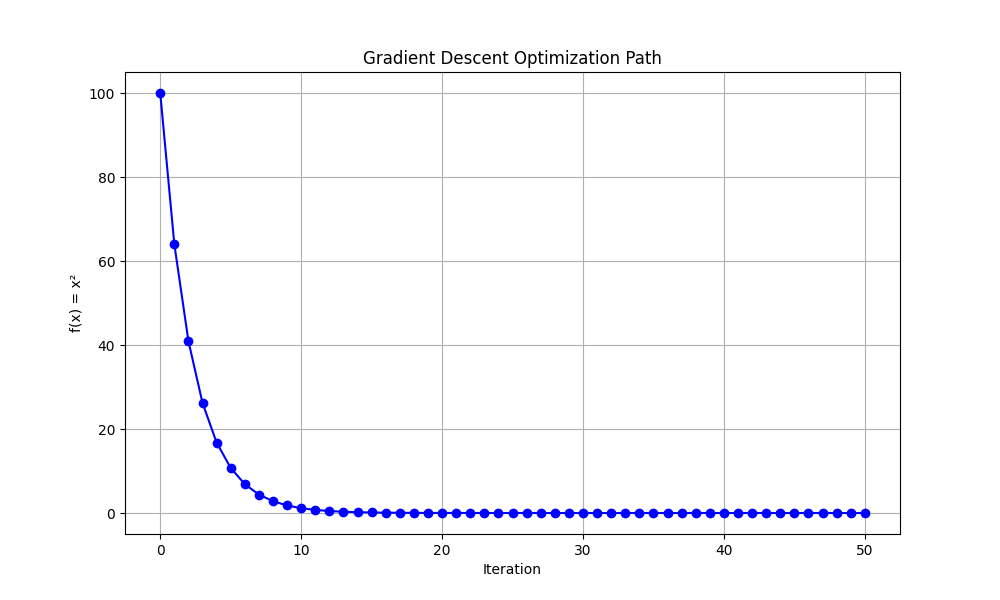
\includegraphics[width=1\textwidth]{chapters/chp3_pics/gd_ex.png}
\caption{\textit{Gradient descent for minimizing the function $f(x) = x^2$}}

    \label{fig:grad_desc_ex}
\end{figure}







\newpage

\lecture{Tangent Planes and Linear Approximations}

\noindent In our exploration of multivariable functions, we have examined how these functions change with respect to their independent variables and how to capture this change using partial derivatives. A central concept in single-variable calculus is the linear approximation of a function near a point, often expressed as the tangent line approximation. In multiple dimensions, the analogous idea is the \textit{tangent plane}, which provides a two-dimensional linear approximation to a surface near a given point. In this lecture, we extend our intuition from single-variable calculus to functions of several variables, focusing on tangent planes and linear approximations. We will also connect these ideas to differentials, which enable us to approximate small changes in a function and apply these approximations to estimate errors in measurements and computations.

\subsection*{From Tangent Lines to Tangent Planes} \index{Tangent Planes}

\noindent Recall from Single-Variable Calculus: you have a function \( y = f(x) \) that is differentiable at a point \( x = a \). If we zoom in very close to the graph of \( f \) at \( (a, f(a)) \), the curve appears almost indistinguishable from a straight line. This line is the \textit{tangent line}, and it gives the best linear approximation to \( f \) near \( x = a \). How do we find this tangent line? We know the slope of the tangent line is given by the derivative \( f'(a) \). The point of tangency is \((a, f(a))\). Combining this information, the equation of the tangent line is:
\[
y \approx f(a) + f'(a)(x - a).
\]

\noindent This linear function approximates \( f(x) \) well for \( x \) near \( a \). In other words, we have a local, linear predictor:
\[
f(x) \approx f(a) + f'(a)(x - a).
\]

\noindent This approximation is not just a convenient guess; it emerges naturally from the definition of the derivative:
\[
f'(a) = \lim_{h \to 0} \frac{f(a+h) - f(a)}{h}.
\]
If we rearrange this definition for small \( h \):
\[
f(a+h) \approx f(a) + f'(a)h,
\]
which is exactly our linear approximation. As \( h \to 0 \), this approximation becomes increasingly accurate. \\

\noindent Now, consider a function of two variables:
\[
z = f(x,y).
\]
We want an analogous concept to the tangent line, but now our domain is two-dimensional, and the graph of \( f \) is a surface in three-dimensional space. Instead of a line, the natural linear approximation to a surface at a given point is a \textit{tangent plane}. \\

\noindent Suppose \( f \) is differentiable at a point \((a,b)\). Differentiability in two dimensions means that as we move from \((a,b)\) to \((a+\Delta x, b+\Delta y)\), the change in \( f \) can be approximated by a linear function of \(\Delta x\) and \(\Delta y\). Let’s express this idea. \\

\noindent In single-variable calculus, differentiability required that:
\[
f(a+h) = f(a) + f'(a)h + \epsilon(h), \quad \text{where } \epsilon(h) \to 0 \text{ as } h \to 0.
\]

\noindent In two-variable calculus, if \( f \) is differentiable at \((a,b)\), we have:
\[
f(a+\Delta x, b+\Delta y) = f(a,b) + f_x(a,b)\Delta x + f_y(a,b)\Delta y + E(\Delta x,\Delta y),
\]
where \( f_x(a,b) \) and \( f_y(a,b) \) are the partial derivatives of \( f \) at \((a,b)\). Here, \(\Delta x\) and \(\Delta y\) are small increments in \( x \) and \( y \) (often denoted by \( h \) and \( k \) in limit definitions). The term \( E(\Delta x,\Delta y) \) is an error term that goes to zero faster than \(\sqrt{(\Delta x)^2 + (\Delta y)^2}\) as \(\Delta x,\Delta y \to 0\). More precisely:
\[
\lim_{(h,k)\to(0,0)} \frac{E(h,k)}{\sqrt{h^2+k^2}} = 0.
\]

\noindent Thus, as \((\Delta x,\Delta y)\) become infinitesimally small, the linear part dominates and the higher-order terms become negligible. This stems from the definition of differentiability, which ensures that the function's behavior is well-approximated by a linear map at the point of tangency.

\begin{figure}[H]
\centering

%---------------------------------------------
% Left figure (Global View):
% To adjust how far the axes extend, you can change the domain for x and y,
% as well as the size of the plot. For instance, 'domain=-3:3' and 'y domain=-3:3'
% control the range of x and y. Also, 'width=7cm, height=7cm' affects the size.
% Increase these values for a bigger view.
%---------------------------------------------
\begin{tikzpicture}
  \begin{axis}[
    width=7cm, height=7cm,         % You can increase these for a bigger plot
    view={60}{30},
    xlabel={$x$}, ylabel={$y$}, zlabel={$z$},
    domain=-3:3, y domain=-3:3,    % Adjust domain range to show more/less of the surface
    samples=30, samples y=30,
    zmin=-1, zmax=1,
    colormap/viridis,
    axis lines=middle,
    grid=major,
    clip=false
  ]
    % Surface: z = sin(x)*cos(y)
    \addplot3[surf, shader=interp, opacity=0.8] {sin(deg(x))*cos(deg(y))};

    % Point of interest (0,0,0)
    \addplot3[mark=*,color=black] coordinates {(0,0,0)};

    % Dotted circle around (0,0)
    \draw[dotted, ultra thick] (axis cs:0,0,0) circle[radius=20pt];

  \end{axis}
\end{tikzpicture}
\hspace{1cm}
%---------------------------------------------
% Right figure (Zoomed-in View):
% Again, to adjust the axes, modify 'domain', 'y domain', and 'width/height'.
% For example, to zoom in more, decrease the domain range; to see more detail, 
% increase samples.
%---------------------------------------------
\begin{tikzpicture}
  \begin{axis}[
    width=7cm, height=7cm,         % Increase for a bigger plot if desired
    view={60}{30},
    xlabel={$x$}, ylabel={$y$}, zlabel={$z$},
    domain=-0.3:0.3, y domain=-0.3:0.3,  % Adjust these for how 'zoomed in' the view is
    samples=30, samples y=30,
    zmin=-0.1, zmax=0.1,
    colormap/viridis,
    axis lines=middle,
    grid=major
  ]
    % Surface near (0,0): z=sin(x)*cos(y)
    \addplot3[
      surf,
      shader=interp,
      opacity=0.8
    ] {sin(deg(x))*cos(deg(y))};

    % Point of interest (0,0,0)
    \addplot3[mark=*,color=black] coordinates {(0,0,0)};

  \end{axis}
\end{tikzpicture}

\caption{\textit{Left: A global view of $z=\sin(x)\cos(y)$ with a dotted region around $(0,0)$. 
Right: A zoomed-in view of the same surface near $(0,0)$, where it appears nearly flat.}}
\end{figure}




\noindent Focusing only on the linear part gives:
\[
f(a+\Delta x, b+\Delta y) \approx f(a,b) + f_x(a,b)\Delta x + f_y(a,b)\Delta y.
\]

\noindent Setting \( x = a + \Delta x \) and \( y = b + \Delta y \), we rewrite this as:
\[
f(x,y) \approx f(a,b) + f_x(a,b)(x - a) + f_y(a,b)(y - b).
\]

\noindent This defines a plane:
\[
z = f(a,b) + f_x(a,b)(x - a) + f_y(a,b)(y - b).
\]

Let \( z_0 = f(a,b) \). Then we can rewrite this as:
\[
z - z_0 = f_x(a,b)(x - a) + f_y(a,b)(y - b),
\]
which matches the standard form of a plane equation: a constant point \((a,b,z_0)\) plus linear terms in \((x-a)\) and \((y-b)\). Here, the ``slopes'' \( f_x(a,b) \) and \( f_y(a,b) \) serve as the coefficients that determine the plane’s tilt in the \( x \)- and \( y \)-directions. In other words, this \textbf{tangent plane} at \((a,b,f(a,b))\) just grazes the surface at that point and provides the best linear approximation, making the surface and the plane virtually indistinguishable when we are very close to \((a,b)\). Below we have an example of a plane tangent to a surface:

\noindent This is powerful: it means we can approximate a complicated surface near any point with a simple plane. If we know the function value and its partial derivatives at one point, we can estimate the function at nearby points without recomputing---an idea that underpins error estimation, numerical methods, and optimization.\\ \\

%---------------------------------------------
% Tangent Plane for f(x,y) = x^2 + y^2 at (1,1)
%---------------------------------------------
\begin{figure}[H]
\centering
\begin{tikzpicture}
  \begin{axis}[
    view={60}{30},
    xlabel={$x$}, ylabel={$y$}, zlabel={$z$},
    domain=-0.5:2.5,
    y domain=-0.5:2.5,
    samples=30,
    samples y=30,
    width=10cm, height=8cm,
    zmin=0, zmax=8,
    grid=major,
    colormap/viridis,
    ztick={0,2,4,6,8}
  ]

    % Plot the surface f(x,y) = x^2 + y^2
    \addplot3[
      surf,
      opacity=0.5,
      shader=interp,
      domain=0:2,
      y domain=0:2,
    ] {x^2 + y^2};

    % Point of tangency (1,1)
    \addplot3[mark=*,color=black] coordinates {(1,1,2)};

    % Compute tangent plane at (1,1):
    % f_x=2x, f_y=2y at (1,1) => f_x=2, f_y=2
    % f(1,1)=1+1=2
    % Tangent plane: z = 2 + 2(x-1) + 2(y-1) = 2x+2y-2
    \addplot3[
      domain=0:2,
      y domain=0:2,
      surf,
      opacity=0.5,
      colormap/cool,
    ] {2*x+2*y-2};

    % Labels
    \node at (axis cs:1,1,2) [anchor=south east] {$(1,1,2)$};
    \node at (axis cs:1,1,8) [anchor=north] {$z=x^2+y^2$};
    \node at (axis cs:1.5,0.5,1) [anchor=south] {Tangent Plane};
  \end{axis}
\end{tikzpicture}
\caption{\textit{Tangent plane to $z=x^2+y^2$ at the point $(1,1,2)$.}}
\end{figure}

\exampleline
\begin{example}
Find the equation of the tangent plane to the surface
\[
z = f(x,y) = x^2 - 3xy + 4y^2
\]
at the point \((2,1)\).

\begin{solution}
First, we need the partial derivatives of \( f \) with respect to \( x \) and \( y \):
\[
f_x(x,y) = 2x - 3y, \quad f_y(x,y) = -3x + 8y.
\]

Evaluate these at \((2,1)\):
\[
f_x(2,1) = 2(2) - 3(1) = 4 - 3 = 1, \quad f_y(2,1) = -3(2) + 8(1) = -6 + 8 = 2.
\]

Also, find \( f(2,1) \):
\[
f(2,1) = (2)^2 - 3(2)(1) + 4(1)^2 = 4 - 6 + 4 = 2.
\]

The tangent plane is given by:
\[
z = f(2,1) + f_x(2,1)(x - 2) + f_y(2,1)(y - 1).
\]

Substitute the values:
\[
z = 2 + 1(x - 2) + 2(y - 1).
\]

Simplify:
\[
z = 2 + (x - 2) + 2y - 2 = x + 2y - 2.
\]

Thus, the equation of the tangent plane is:
\[
z = x + 2y - 2.
\]
It doesn't get much harder than that!
\end{solution}
\end{example}
\exampleline


\subsection*{Generalization to Higher Dimensions and Hyperplanes} \index{Hyperplanes}

\noindent The concept of tangent planes naturally extends to functions of more than two variables. For a function
\[
f: \mathbb{R}^n \to \mathbb{R},
\]
differentiability at a point \(\mathbf{a} = (a_1, a_2, \ldots, a_n)\) means that we can approximate \( f \) near \(\mathbf{a}\) by a linear function involving the partial derivatives with respect to each of the \( n \) variables. Specifically, we have:
\[
f(\mathbf{a} + \Delta \mathbf{x}) = f(\mathbf{a}) + \nabla f(\mathbf{a}) \cdot \Delta \mathbf{x} + E(\Delta \mathbf{x}),
\]
where \(\nabla f(\mathbf{a})\) is the gradient vector of \( f \) at \(\mathbf{a}\), and \(\Delta \mathbf{x}\) is a small displacement vector in \(\mathbb{R}^n\). Ignoring the small error term, we obtain a linear approximation:
\[
f(\mathbf{a} + \Delta \mathbf{x}) \approx f(\mathbf{a}) + \nabla f(\mathbf{a}) \cdot \Delta \mathbf{x}.
\]

\noindent The set of points \((\mathbf{x}, z)\) in \(\mathbb{R}^{n+1}\) satisfying
\[
z = f(\mathbf{a}) + \nabla f(\mathbf{a}) \cdot (\mathbf{x}-\mathbf{a})
\]
defines a \textit{tangent hyperplane} to the graph of \( f \) at \(\mathbf{a}\). For \( n=1 \), this hyperplane is just a line (the tangent line). For \( n=2 \), it’s a plane (the tangent plane). For \( n>2 \), the object is an \(n\)-dimensional hyperplane—a direct generalization of the idea of “flat” linear approximations to higher dimensions.

\subsubsection*{Hyperplanes in Machine Learning:}  \index{Hyperplanes}
In machine learning, hyperplanes appear in various contexts, notably in classification tasks. For instance, linear classifiers such as Support Vector Machines (SVMs) or simple linear regression models rely on hyperplanes to separate data points or fit data. Consider a binary classification problem in \(\mathbb{R}^n\). A linear classifier tries to find a hyperplane:
\[
\mathbf{w} \cdot \mathbf{x} + b = 0,
\]
that best separates data points of different classes. Here, \(\mathbf{w}\) is a weight vector (analogous to the gradient vector), and \( b \) is a bias term (analogous to a constant offset). The hyperplane defined by this equation divides \(\mathbb{R}^n\) into two half-spaces, and the classifier assigns points on one side to one class and points on the other side to the opposite class. \\

\noindent The connection between the tangent plane (or hyperplane) in calculus and the hyperplanes in machine learning is conceptually significant. Both represent the idea of using linear structures to approximate or make decisions about more complex, nonlinear situations. In calculus, the tangent hyperplane locally approximates a nonlinear function. In machine learning, a hyperplane provides a simple linear boundary in a potentially high-dimensional space. Although the goals differ—approximation of functions vs. classification of points—the underlying mathematical object (a linear function defining a hyperplane) is fundamentally the same.

\subsubsection*{A Simple Linear Classifier in 2D} \index{Linear Classifier}

\noindent Consider a simple binary classification task in two dimensions. Suppose each data point is represented by a vector \(\mathbf{x} = (x_1, x_2)\) in \(\mathbb{R}^2\), and we want to classify it into one of two classes, say ``A" or ``B". A very basic linear classifier can be written as:
\[
\mathbf{w} \cdot \mathbf{x} + b = 0,
\]
where \(\mathbf{w} = (w_1, w_2)\) is a weight vector and \( b \) is a bias term. \\

\noindent This equation defines a line in the \( x_1x_2 \)-plane, which is a 1-dimensional hyperplane (since a line is a hyperplane in \(\mathbb{R}^2\)). The classifier assigns points on one side of the line to class A and points on the other side to class B. Specifically:
\[
\mathbf{w} \cdot \mathbf{x} + b > 0 \implies \text{Class A}, \quad \mathbf{w} \cdot \mathbf{x} + b < 0 \implies \text{Class B}.
\]

\noindent For example, let’s choose \( \mathbf{w} = (1, -2) \) and \( b = 1 \). The decision boundary is:
\[
1 \cdot x_1 + (-2) \cdot x_2 + 1 = 0 \implies x_1 - 2x_2 + 1 = 0.
\]

\noindent Rearranging:
\[
x_1 = 2x_2 - 1.
\]

\noindent This line divides the plane into two regions:
\[
x_1 > 2x_2 - 1 \implies \mathbf{x} \text{ is in Class A}, \quad x_1 < 2x_2 - 1 \implies \mathbf{x} \text{ is in Class B}.
\]

\begin{figure}[H]
\centering
\begin{tikzpicture}
  \begin{axis}[
    axis lines=middle,
    xlabel={$x_2$}, ylabel={$x_1$},
    xmin=-2, xmax=3, ymin=-2, ymax=4,
    grid=major,
    width=10cm, height=7cm,
  ]

    % Decision boundary line: x_1 = 2x_2 - 1
    \addplot[domain=-2:3, samples=100, thick, red] {2*x -1};

    % Some sample points on different sides
    \addplot[mark=*,blue] coordinates {(0,0.5)};  % Check sign: 0.5 - 2*0 +1=1.5>0 => A
    \node[blue, anchor=south] at (axis cs:0,0.5) {A};
    
    \addplot[mark=*,blue] coordinates {(1,2.5)};  % Check: 2.5 - 2*1+1=2.5-2+1=1.5>0 => A
    \node[blue, anchor=south] at (axis cs:1,2.5) {A};
    
    \addplot[mark=*,purple] coordinates {(0,-1)};   % Check: -1 -2*(0)+1=0 => on boundary
    \node[purple, anchor=north] at (axis cs:0,-1) {On boundary};
    
    \addplot[mark=*,green!50!black] coordinates {(1,-1)}; % Check: -1 - 2*(1)+1=-1-2+1=-2<0 => B
    \node[green!50!black, anchor=north] at (axis cs:1,-1) {B};

    \addplot[mark=*,green!50!black] coordinates {(2,0)};   % Check:0 -2*(2)+1=0-4+1=-3<0 => B
    \node[green!50!black, anchor=north] at (axis cs:2,0.6) {B};

  \end{axis}
\end{tikzpicture}
\caption{\textit{A simple linear classifier in $\mathbb{R}^2$. The line $x_1 = 2x_2 - 1$ separates the plane into two classes. Points labeled A fall on one side, and points labeled B on the other.}}
\end{figure}

\noindent Here, the concept of a hyperplane from calculus—a linear construct that approximates behavior locally—appears in a machine learning context as a global decision boundary. Although the goal is different (classifying points rather than approximating a function at a point), the mathematical form is similar: a linear equation representing a flat boundary in space. This exemplifies how linear mathematical objects like lines, planes, and hyperplanes serve as foundational building blocks across various domains, from analyzing rates of change in calculus to making decisions in machine learning.


\subsection*{Linear Approximations: The Bridge Between Theory and Practice} \index{Linear Approximation}

\noindent Just as we used the tangent line in one dimension to approximate function values near a point, the tangent plane in two dimensions provides a linear approximation to \( f(x,y) \) near \((a,b)\). This approximation is extremely useful in many contexts:
\begin{itemize}
    \item \textbf{Estimating Values:} If we know \( f(a,b) \) and the partial derivatives at \((a,b)\), we can estimate \( f(x,y) \) for \((x,y)\) close to \((a,b)\) without computing \( f \) directly.
    \item \textbf{Differentials:} We define differentials \( dx \) and \( dy \) as small increments in \( x \) and \( y \). Then the differential \( df \) at \((a,b)\) is:
    \[
    df = f_x(a,b) dx + f_y(a,b) dy.
    \]
    This quantity \( df \) represents the best linear prediction for the actual change \(\Delta f = f(a+dx,b+dy)-f(a,b)\) for small changes \( dx \) and \( dy \). It is the multivariable extension of \( dy = f'(a)dx \) from single-variable calculus.
    \item \textbf{Error Estimation:} Suppose you measure \( x \) and \( y \) with some small possible errors \(\Delta x\) and \(\Delta y\). Using the tangent plane approximation, you can estimate how these errors propagate into \( f \):
    \[
    \Delta f \approx f_x(a,b)\Delta x + f_y(a,b)\Delta y.
    \]
    This lets you gauge how sensitive the function is to changes in its input variables.
\end{itemize}

\noindent Thus, the progression is:
\[
\text{Single variable: Tangent line} \implies f(x) \approx f(a) + f'(a)(x-a).
\]
\[
\text{Two variables: Tangent plane} \implies f(x,y) \approx f(a,b) + f_x(a,b)(x-a) + f_y(a,b)(y-b).
\]

\noindent This parallel structure shows that the concept of a linear approximation—so central in understanding functions in one dimension—scales naturally to higher dimensions, giving us a powerful geometric and analytic tool to approximate and understand the behavior of multivariable functions near any given point.

\subsubsection*{Beyond the Linear Approximation:} 

In some situations, the linear approximation may not provide sufficient information. For instance, if \(\nabla f(a,b) = \mathbf{0}\) (all first-order partial derivatives vanish), then the tangent plane is flat and does not reveal how \( f \) changes for small deviations from \((a,b)\). In such cases, we look to higher-order approximations, much like we use second- or third-order Taylor polynomials in single-variable calculus. \\

\noindent In two variables, a second-order approximation (also known as the quadratic approximation) includes second partial derivatives:
\[
\begin{split}
f(x,y) &\approx f(a,b) + f_x(a,b)(x-a) + f_y(a,b)(y-b) \\
&\quad + \tfrac{1}{2}\bigl[f_{xx}(a,b)(x-a)^2 + 2f_{xy}(a,b)(x-a)(y-b) + f_{yy}(a,b)(y-b)^2\bigr].
\end{split}
\]

\noindent These higher-order terms capture curvature and more subtle changes in the function. They can distinguish between extrema and provide more accurate estimates when larger changes in \( x \) and \( y \) occur. \\

\noindent While the linear approximation (tangent plane) is often the first and most accessible tool, knowing that higher-order expansions exist broadens your ability to model and understand complex phenomena. Whether adjusting manufacturing parameters, forecasting economic indicators, or analyzing stability in physical systems, having the option to include second-order (or higher) terms allows for richer, more nuanced approximations.

\exampleline
\begin{example}
A drone mapping a field captures the elevation of the terrain using the function:
\[
f(x,y) = 1000 - (x-25)^2 - \tfrac{1}{2}(y-50)^2,
\]
where \(x\) and \(y\) are coordinates in meters, and \(f(x,y)\) gives the elevation in meters. At the reference point \((25,50)\), the elevation is \(f(25,50) = 1000\) meters. Suppose the drone slightly shifts its measurement to \((26,48)\).

\begin{enumerate}
    \item Use a first-order (linear) approximation at \((25,50)\) to estimate the elevation at \((26,48)\).
    \item Compute the actual elevation at \((26,48)\) and discuss why the linear approximation fails.
    \item Suggest and compute a second-order approximation to improve the estimate.
\end{enumerate}

\begin{solution}
\begin{enumerate}
    \item \textbf{First-Order Approximation:} \index{First-Order Approximation}
    
    The first-order approximation uses the tangent plane to estimate elevation. The general formula for the first-order (linear) approximation of a function \( f(x,y) \) at a reference point \( (a,b) \) is:
    \[
    f(x,y) \approx f(a,b) + f_x(a,b)(x - a) + f_y(a,b)(y - b)
    \]
    For the given function:
    \[
    f(x,y) = 1000 - (x-25)^2 - \tfrac{1}{2}(y-50)^2,
    \]
    the partial derivatives are:
    \[
    f_x(x,y) = -2(x-25), \quad f_y(x,y) = -(y-50).
    \]
    At the reference point \((25,50)\):
    \[
    f_x(25,50) = -2(25-25) = 0, \quad f_y(25,50) = -(50-50) = 0.
    \]
    Substituting these values into the first-order approximation formula:
    \[
    f(x,y) \approx f(25,50) + 0 \cdot (x - 25) + 0 \cdot (y - 50) = 1000.
    \]
    Since both partial derivatives are zero at \((25,50)\), the linear approximation is a constant:
    \[
    f(x,y) \approx 1000.
    \]
    Using this approximation, the predicted elevation at \((26,48)\) is:
    \[
    f(26,48) \approx 1000.
    \]
    
    \item \textbf{Actual Elevation:}
    
    Compute the exact elevation at \((26,48)\):
    \[
    f(26,48) = 1000 - (26-25)^2 - \tfrac{1}{2}(48-50)^2.
    \]
    Simplify step by step:
    \[
    f(26,48) = 1000 - 1 - \tfrac{1}{2}(4) = 1000 - 1 - 2 = 997.
    \]
    The actual elevation is \(997\) meters, but the linear approximation predicted \(1000\). The error occurs because the tangent plane is flat at \((25,50)\), failing to capture the curvature of the terrain. In fact, our scheme will predict everything to be flat since $f(25,50)$ is constant. If we are very far up the terrain when this approximation is made, it'll only get much worse the farther out we go.
    
    \item \textbf{Second-Order Approximation:}  \index{Second-Order Approximation}
    
    To account for curvature, we use a second-order Taylor approximation:
\[
\begin{split}
f(x,y) &\approx f(a,b) + f_x(a,b)(x-a) + f_y(a,b)(y-b) \\
&\quad + \tfrac{1}{2}\bigl[f_{xx}(a,b)(x-a)^2 + 2f_{xy}(a,b)(x-a)(y-b) + f_{yy}(a,b)(y-b)^2\bigr].
\end{split}
\]
Compute the second derivatives:
    \[
    f_{xx}(x,y) = -2, \quad f_{yy}(x,y) = -1, \quad f_{xy}(x,y) = 0.
    \]
    The second-order approximation is:
\[
\begin{split}
f(x,y) &\approx f(25,50) + \tfrac{1}{2}\bigl[f_{xx}(25,50)(x-25)^2 \\
&\quad + 2f_{xy}(25,50)(x-25)(y-50) \\
&\quad + f_{yy}(25,50)(y-50)^2\bigr].
\end{split}
\]

    Substituting the derivatives and evaluating at \((26,48)\):
    \[
    f(26,48) \approx 1000 + \tfrac{1}{2}\bigl[-2(1)^2 + 0 + (-1)(-2)^2\bigr].
    \]
    Simplify:
    \[
    f(26,48) \approx 1000 + \tfrac{1}{2}(-2 - 4) = 1000 - \tfrac{6}{2} = 1000 - 3 = 997.
    \]
    The second-order approximation recovers the actual value, showing that considering curvature is crucial when first-order terms vanish.
    
    \item \textbf{Conclusion:}
    
    For flat terrain at a critical point (where the gradient is zero), higher-order terms reveal how the elevation changes. The second-order approximation includes curvature information, making it essential for accurate predictions in such cases.
\end{enumerate}
\end{solution}
\end{example}
\exampleline




\newpage

\lecture{Extrema and Critical Points}

\noindent One of the central themes in calculus is understanding where a function attains its greatest or least values. In single-variable calculus, this investigation led us to examine critical points—points where the derivative vanishes—and to use second-derivative tests to classify the nature of these points. These critical points allowed us to identify local maxima, local minima, and to note where the function’s concavity changes (potentially at points of inflection). Such insights gave us a clear understanding of the ``shape" of a curve along a one-dimensional axis. Because plotting is more challenging in higher dimensions, any analogy or simpler scenario that helps us visualize these concepts is useful. Not only this, but for optimization we will find extrema to be a cornerstone, just as we saw in single variable calculus. \\

\noindent As we move to functions of several variables, the problem becomes richer and more complex. Instead of analyzing a single input-output relationship along a line, we now consider surfaces (or even higher-dimensional objects) defined by multiple input variables. The notion of ``increasing" or ``decreasing" can no longer be grasped by simply looking to the left or right. We must consider changes in all possible directions around a point (often referred to as examining a \textit{neighborhood}). Consequently, the identification and classification of maxima, minima, and other special points (such as saddle points) demand more sophisticated tools and a broader conceptual framework. 

\subsection*{Single-Variable Concepts and Their Limitations} \index{Critical Points}

\noindent Let’s start by recalling what we know from single-variable calculus. For a differentiable function \( f: \mathbb{R} \to \mathbb{R} \):
\begin{itemize}
    \item A \textbf{critical point} \( x = a \) is where \( f'(a) = 0 \) or \( f'(a) \) does not exist.
    \item At such points, the function might have a local maximum or minimum, or it might simply change its curvature, suggesting a point of inflection (though not necessarily an extremum).
    \item To distinguish maxima and minima from other behaviors, we use the \textbf{second derivative test}:
    \begin{itemize}
        \item[$\circ$] If \( f''(a) > 0 \), the function is concave up at \( a \), typically indicating a local minimum.
        \item[$\circ$] If \( f''(a) < 0 \), the function is concave down at \( a \), typically indicating a local maximum.
        \item[$\circ$] If \( f''(a) = 0 \), the test is inconclusive and the behavior around \( a \) requires further investigation.
    \end{itemize}
    \item A \textbf{point of inflection} occurs at \( x = a \) if the function changes concavity (from concave up to concave down, or vice versa) at that point. To identify such points:
    \begin{itemize}
        \item[$\circ$] Compute \( f''(x) \) and find where \( f''(x) = 0 \) or \( f''(x) \) does not exist.
        \item[$\circ$] Check the sign of \( f''(x) \) on either side of \( x = a \). A change in sign confirms a point of inflection.
    \end{itemize}
\end{itemize}


%---------------------------
% A Basic Figure Demonstrating Extrema in One Variable
%---------------------------
\begin{figure}[H]
\centering
\begin{tikzpicture}
  \begin{axis}[
    axis lines=middle,
    xlabel={$x$}, ylabel={$y$},
    xmin=-3.5, xmax=3.5,
    ymin=-4, ymax=4,
    grid=major,
    width=10cm, height=6cm,
    domain=-3:3,
    samples=200,
  ]
    % Example function: f(x) = x^3 - 3x
    % f'(x)=3x^2 - 3; f''(x)=6x
    % Critical points: f'(x)=0 => 3x^2-3=0 => x^2=1 => x=±1.
    % At x=1, f''(1)=6(1)=6>0 -> local min at (1,1^3-3*1=1-3=-2)
    % At x=-1, f''(-1)=6(-1)=-6<0 -> local max at (-1, -(-3)=2)
    % Inflection point: f''(x)=0 => x=0, y=0^3-3*0=0
    \addplot[blue, thick] {x^3 - 3*x};

    % Mark critical points
    \addplot[mark=*, only marks, color=red] coordinates {(-1,2)}; % local max
    \addplot[mark=*, only marks, color=red] coordinates {(1,-2)}; % local min
    \addplot[mark=*, only marks, color=green] coordinates {(0,0)}; % inflection

    % Labels for points
    \node[above left, red] at (axis cs:-1,2) {Local Max};
    \node[below right, red] at (axis cs:1,-2) {Local Min};
    \node[above, green] at (axis cs:0,0) {Inflection Point};

  \end{axis}
\end{tikzpicture}
\caption{\textit{A single-variable function \(f(x)=x^3-3x\) illustrating a local maximum, local minimum, and an inflection point. The critical points at \(x=-1\) and \(x=1\) correspond to a local maximum and local minimum, respectively, while \(x=0\) is a point of inflection where the curvature changes.}}
\end{figure}

\noindent In the figure above, we see an example function \( f(x)=x^3 - 3x \) that has:
\begin{itemize}
    \item A local maximum at \( x=-1 \).
    \item A local minimum at \( x=1 \).
    \item An inflection point at \( x=0 \), where the graph changes from concave down to concave up.
\end{itemize}


\noindent These principles form the basis of understanding how functions behave near critical points in one dimension. However, when we move to multiple variables, these ideas must be generalized. Instead of a single derivative, we have partial derivatives. Instead of a single second derivative, we have a matrix of second-order partial derivatives (the Hessian). Instead of a single direction to check for concavity changes, we must consider changes in every direction. Because Linear Algebra is not a prerequisite to Multivariate Calculus, we will take this slow, don't worry. The complexity and richness of these scenarios make the transition from one-dimensional to multivariable calculus both challenging and rewarding. \\


\noindent The framework above allowed us to solve a variety of one-dimensional optimization problems. However, this approach heavily relies on the fact that there's only one independent variable. Extending these ideas to multiple variables introduces several challenges:
\begin{itemize}
    \item \textbf{Directionality:} In one dimension, you look left and right. In multiple dimensions, you must consider infinitely many directions from a point.
    \item \textbf{Multidimensional Curvature:} Instead of a single second derivative, we have a whole matrix of second derivatives (the Hessian).
    \item \textbf{Types of Critical Points:} With more directions come new types of stationary behavior. In particular, \textit{saddle points} arise, which are not maxima or minima, but still have zero gradient.
\end{itemize}

\subsection*{Extrema in Several Variables} \index{Extrema in Several Variables}


\noindent Generalizing some of the concepts to higher dimensions comes naturally enough with the notational conventions we have established in previous lectures. Consider a function \( f: \mathbb{R}^n \to \mathbb{R} \). We say that \( \mathbf{a} \in \mathbb{R}^n \) is an \textbf{extremum} of \( f \) if \( f(\mathbf{a}) \) is a maximum or minimum value of \( f \) in some sense. As in one dimension, we distinguish between:
 \index{Local Extrema} \index{Local Minima} \index{Local Maxima}
\begin{itemize}
    \item \textbf{Local Maximum in \(\mathbb{R}^n\)}: \( f(\mathbf{a}) \) is greater than or equal to \( f(\mathbf{x}) \) for all points \(\mathbf{x}\) in some ``small neighborhood" around \(\mathbf{a}\).
    \item \textbf{Local Minimum in \(\mathbb{R}^n\)}: \( f(\mathbf{a}) \) is less than or equal to \( f(\mathbf{x}) \) for all points \(\mathbf{x}\) in a small neighborhood around \(\mathbf{a}\).
    \item \textbf{Global Maximum/Minimum}: The value at \(\mathbf{a}\) is the supreme representative—no points in the entire domain beat it (for a max) or undercut it (for a min).
\end{itemize}
\noindent Below we see a 3D plot displaying all these extrema. Because we choose a function on a region $R = [-5,5] \times [-5,5]$ that has no division, and thus no points in the plot that go off to $\pm \infty$, we are guaranteed global extrema due the closed and bounded nature of the conditions. We will learn about this as the Extreme Value Theorem for multivariate functions.

\begin{figure}[H]
\centering
\begin{tikzpicture}
  \begin{axis}[
    view={60}{30},
    domain=-5:5, 
    domain y=-5:5,
    xlabel=$x$, ylabel=$y$, zlabel={$f(x,y)$},
    samples=41,
    width=10cm,
    height=8cm,
    legend style={at={(1.05,1)},anchor=north west}
  ]
    % Surface
    \addplot3[
      surf,
      shader=interp,
      opacity=0.7,
      colormap/viridis
    ] {sin(deg(x))*sin(deg(y))*exp(-0.1*(x^2+y^2))};
    \addlegendentry{Surface}

    % Global maxima (max=triangle)
    \addplot3[blue,mark=triangle*,only marks,mark size=2pt]
    coordinates {
      (-1.3154,-1.3154,0.6623)
      (1.3154,1.3154,0.6623)
    };
    \addlegendentry{Global max}

    % Global minima (min=circle)
    \addplot3[blue,mark=o,only marks,mark size=2pt]
    coordinates {
      (1.3154,-1.3154,-0.6623)
      (-1.3154,1.3154,-0.6623)
    };
    \addlegendentry{Global min}

    % Local maxima (interior) (max=triangle)
    \addplot3[red,mark=triangle*,only marks,mark size=1.5pt]
    coordinates {
      (1.3154,-4.0330,0.1245)
      (-4.0330,1.3154,0.1245)
      (4.0330,-1.3154,0.1245)
      (-1.3154,4.0330,0.1245)
    };
    \addlegendentry{Local max (interior)}

    % Local minima (interior) (min=circle)
    \addplot3[red,mark=o,only marks,mark size=1.5pt]
    coordinates {
      (4.0330,1.3154,-0.1245)
      (1.3154,4.0330,-0.1245)
      (-1.3154,-4.0330,-0.1245)
      (-4.0330,-1.3154,-0.1245)
    };
    \addlegendentry{Local min (interior)}

    % Local maxima (boundary) at (-5,-5) and (5,5) (max=triangle)
    \addplot3[green!70!black,mark=triangle*,only marks,mark size=1.5pt]
    coordinates {
      (-5,-5,0.006195)
      (5,5,0.006195)
    };
    \addlegendentry{Local max (boundary)}

    % Local minima (boundary) at (5,-5) and (-5,5) (min=circle)
    \addplot3[green!70!black,mark=o,only marks,mark size=1.5pt]
    coordinates {
      (5,-5,-0.006195)
      (-5,5,-0.006195)
    };
    \addlegendentry{Local min (boundary)}

  \end{axis}
\end{tikzpicture}
\caption{\textit{The surface plot of $f(x,y) = \sin(x)\sin(y)e^{-0.1(x^2 + y^2)}$ with annotated extrema. No laughing, please.}}
\label{fig:extrema_ex}
\end{figure}

\noindent However, unlike the single-variable case, ``small neighborhood” is not just an interval around a point. In \(\mathbb{R}^n\), you can approach a point from infinitely many directions. There can be ``flat” regions where the function doesn't change for a while, disconnected parts of the domain, and directions in which the function heads off to infinity (no global extrema exist). Thus, while the idea of local and global maxima and minima transfers directly, the complexity of higher dimensions makes the identification and classification of these points more subtle.

\subsubsection*{A Rigorous Approach}

Before we dive into the rigor, we need to define the concepts of \textbf{open sets}, \textbf{closed sets}, \textbf{balls}, and \textbf{compactness}. Understanding these definitions is crucial for formalizing our discussions on neighborhoods and extrema in multiple dimensions.

\begin{itemize}
    \item \textbf{Open Set}: \index{Open Sets} A set \( U \subset \mathbb{R}^n \) is called \textit{open} if, for every point \( \mathbf{a} \in U \), you can move a little bit in any direction from \( \mathbf{a} \) and still stay within \( U \). In other words, there are no ``edge" points included in \( U \). This is essentially the higher dimensional analog of an open interval $(a,b)$.
    
    \item \textbf{Closed Set}: \index{Closed Sets} A set \( C \subset \mathbb{R}^n \) is called \textit{closed} if it includes all its boundary points. This means that if you have a sequence of points within \( C \) that gets closer and closer to some point \( \mathbf{x} \), then \( \mathbf{x} \) is also included in \( C \). This is essentially the higher dimensional analog of a closed interval $[a,b]$.


%---------------------------------------
% Illustration of disjoint open set U and closed set C
%---------------------------------------
\begin{figure}[H]
\centering
\begin{tikzpicture}
  % Open Set U
  \begin{axis}[
    width=6cm, height=6cm,           % Smaller size
    axis lines=none,                 % Remove axes
    clip=false,                      % Allow plotting outside axis bounds
    xlabel style={font=\small}, ylabel style={font=\small},
    tick label style={font=\small},
    title={Open Set $U$},            % Title for open set
    title style={font=\small, at={(0.5,-0.1)}, anchor=north}, % Center title below plot
    ]
    % Dotted boundary
    \addplot[
      domain=0:360,
      samples=100,
      dashed,
      thick
    ] (
      {cos(x)},
      {sin(x)}
    );
  \end{axis}

  % Closed Set C
  \begin{axis}[
    at={(7cm,0)},                    % Place side by side with some separation
    width=6cm, height=6cm,           % Smaller size
    axis lines=none,                 % Remove axes
    clip=false,                      % Allow plotting outside axis bounds
    xlabel style={font=\small}, ylabel style={font=\small},
    tick label style={font=\small},
    title={Closed Set $C$},          % Title for closed set
    title style={font=\small, at={(0.5,-0.1)}, anchor=north}, % Center title below plot
    ]
    % Solid boundary
    \addplot[
      domain=0:360,
      samples=100,
      thick
    ] (
      {cos(x)},
      {sin(x)}
    );
  \end{axis}
\end{tikzpicture}
\caption{\textit{Illustration of an open set $U$ with a dotted boundary and a closed set $C$ with a solid boundary.}}
\end{figure}

    
    \item \textbf{Open Ball}: An open ball in \( \mathbb{R}^n \) centered at \( \mathbf{a} \) with radius \( \epsilon \) is the set of all points \( \mathbf{x} \) such that the distance between \( \mathbf{x} \) and \( \mathbf{a} \) is less than \( \epsilon \). It is defined as:
    \[
    B_{\epsilon}(\mathbf{a}) = \left\{ \mathbf{x} \in \mathbb{R}^n \mid \|\mathbf{x} - \mathbf{a}\| < \epsilon \right\}.
    \]
    
    \item \textbf{Compact Set}: \index{Compact Sets} A set \( D \subset \mathbb{R}^n \) is called \textit{compact} if it is both closed and bounded. This means that \( D \) contains all its boundary points and fits within some finite region of space.
\end{itemize}

\noindent To handle these complexities, we need a more precise definition of what it means to be ``close" to a point in multiple dimensions. In one dimension, being close to \( a \) meant \( |x - a| < \epsilon \) for some \(\epsilon > 0\). In \(\mathbb{R}^n\), we generalize this by using open balls defined by a norm. A standard choice is the Euclidean norm \( \|\cdot\| \), which represents the usual distance between vectors. Thus, we define:
\[
B_{\epsilon}(\mathbf{a}) = \left\{ \mathbf{x} \in \mathbb{R}^n \mid \|\mathbf{x} - \mathbf{a}\| < \epsilon \right\}.
\]
This \( B_{\epsilon}(\mathbf{a}) \) is an \textit{open ball} of radius \(\epsilon\) centered at \( \mathbf{a} \). It serves as the higher-dimensional analogue of a small interval around a point.
\\

\noindent With this notation, we can restate the definitions more rigorously:
\begin{itemize}
    \item \textbf{Local Maximum:} A point \(\mathbf{a}\) is a local maximum of \( f \) if there exists \(\epsilon >0\) such that for all \(\mathbf{x} \in B_{\epsilon}(\mathbf{a})\),
    \[
    f(\mathbf{x}) \leq f(\mathbf{a}).
    \]
    Here, ``all \(\mathbf{x}\) in \( B_{\epsilon}(\mathbf{a})\)" means we are checking every direction and every point sufficiently close to \(\mathbf{a}\).

    \item \textbf{Local Minimum:} A point \(\mathbf{a}\) is a local minimum of \( f \) if there exists \(\epsilon > 0\) such that for all \(\mathbf{x} \in B_{\epsilon}(\mathbf{a})\),
    \[
    f(\mathbf{x}) \geq f(\mathbf{a}).
    \]

    \item \textbf{Global Maximum/Minimum:} These are defined similarly to the single-variable case, but we consider the entire domain. A point \(\mathbf{a}\) is a global maximum if
    \[
    f(\mathbf{x}) \leq f(\mathbf{a}) \text{ for all } \mathbf{x} \in \text{dom}(f).
    \]
    And similarly for a global minimum.
\end{itemize}

\noindent Using these $\epsilon$-ball/neighborhood definitions makes our concepts more robust. For instance, the notion of local extremum now doesn’t depend on the shape of the domain or the peculiarities of how we approach the point \(\mathbf{a}\). Instead, it inherently encodes the idea of “closeness" and “no other nearby points exceeding (or undercutting) the value at \(\mathbf{a}\)." \\

\noindent This refined perspective also ties in with deeper results from real analysis. For example, if \( f \) is continuous on a compact set \( D \subset \mathbb{R}^n \), the Extreme Value Theorem guarantees the existence of global maxima and minima. However, if the domain is not compact, or if \( f \) is not nicely behaved, we may fail to find global extrema. The function may “escape” to infinity in some direction, preventing a global maximum or minimum from forming. 


\subsubsection*{Local vs. Global Extrema} \index{Global Extrema} \index{Global Minima} \index{Global Maxima}

\noindent The \textit{Extreme Value Theorem} from single-variable calculus ensures that if a continuous function is defined on a closed interval, it attains global maxima and minima. In higher dimensions, there is a corresponding result: if \( f \) is continuous on a \textit{compact set} \( D \subset \mathbb{R}^n \) (i.e., \( D \) is closed and bounded), then \( f \) attains both a global maximum and a global minimum on \( D \). However, if the domain is not compact, the situation is more complex:
\begin{itemize}
    \item If the domain is not bounded, \( f \) may ``escape" to infinity, never settling on a highest or lowest value.
    \item If the domain is open or lacks a boundary, local conditions might not guarantee global extremality.
\end{itemize}

\noindent Understanding these nuances is crucial in applications. For example, in optimization problems with constraints, ensuring the constraint set is compact (often via bounding conditions) can help guarantee that a solution (a global extremum) exists. \\

\noindent Consider a two-dimensional function \( f(x,y) \) that forms a surface in \(\mathbb{R}^3\). A local maximum appears like a peak in some \(\epsilon\)-ball around \((a,b)\); a local minimum looks like a valley. If the surface keeps rising as \( x^2+y^2 \to \infty \) (like a giant unbounded mountain), no global maxima exist because we can always find higher points. Similarly, if it keeps going downwards without bound, no global minima exist.



%---------------------------------------
% Insert a figure illustrating a local maximum on a surface with an epsilon ball around the global max
%---------------------------------------
\begin{figure}[H]
\centering
\begin{tikzpicture}
  \pgfmathsetmacro{\plotwidth}{13}  % Adjustable width in cm
  \pgfmathsetmacro{\plotheight}{13} % Adjustable height in cm
  \begin{axis}[
    view={45}{30},                     % Adjust the viewing angle
    xlabel={$x$}, ylabel={$y$}, zlabel={$z$},
    axis lines=middle,                 % Only draw the axes through the middle
    domain=-1:1, y domain=-1:1,
    samples=50, samples y=50,          % Increase sample density for better resolution
    width=\plotwidth cm, height=\plotheight cm, % Use adjustable dimensions
    colormap/viridis,
    zmin=0, zmax=3,
    clip=true,                          % Ensure plot elements are clipped to the axis area
    enlargelimits=false,                % Prevent automatic enlargement of plot limits
    tick style={thick, black},          % Thicker ticks for better visibility
    tick label style={font=\small},     % Consistent font size for tick labels
    xlabel style={font=\small},         % Consistent font size for labels
    ylabel style={font=\small},
    zlabel style={font=\small},
    axis equal image,                   % Ensure equal scaling for all axes
    ]
      % Plot the surface with a local maximum at (0,0,3)
      \addplot3[
        surf,
        opacity=0.8,
        shader=interp,                    % Smooth shading for better appearance
      ] 
      {3 - 3*(x^2 + y^2)};
      
      % Mark the top point (0,0,3) with a red dot
      \addplot3[
        only marks,
        mark=*,
        color=red,
        mark size=4pt,                    % Increase marker size for visibility
      ] 
      coordinates {(0,0,3)};
      
      % Define epsilon
      \pgfmathsetmacro{\eps}{0.3}
      
      % Add an epsilon-ball (sphere) around the global maximum (0,0,3)
      \addplot3[
        surf,
        opacity=0.1,                      % Increased transparency
        color=blue,
        samples=30,                       % Increase sphere resolution
        domain=0:360,
        y domain=0:180,
      ]
      (
        {\eps * sin(y) * cos(x)},
        {\eps * sin(y) * sin(x)},
        {3 + \eps * cos(y)}
      );
      
      % Add a label for the epsilon ball
      \node at (axis cs:\eps,-.3,2.7) [anchor=west, color=blue, font=\small] {$B_\epsilon([0,0,3])$};
  \end{axis}
\end{tikzpicture}
\caption{\textit{A surface with a global maximum at the origin. The red dot marks the global maximum at $(0, 0, 3)$. The blue semi-transparent sphere represents a $B_\epsilon([0,0,3])$, illustrating a neighborhood within which no other points have a higher value. As we move away from the origin, the surface descends, ensuring that the global maximum is maintained within the $B_\epsilon([0,0,3])$.}}
\end{figure}





\noindent In the figure above, we see a simple example: \( f(x,y)=3 - 3(x^2+y^2) \) has a local maximum at \((0,0)\) where \( f(0,0)=3 \). In fact, this is also a global maximum since the function decreases as we move away from \((0,0)\), approaching negative infinity without bound. If we had a function that only rose at the origin and flattened out or grew in other directions, we might not have any global maxima or minima, just local ones. 



\exampleline
\begin{example}
Consider the Extreme Value Theorem (EVT) \index{Extreme Value Theorem} in the context of multivariable calculus, which states that if a function \( f: \mathbb{R}^n \to \mathbb{R} \) is continuous on a \textit{compact} set \( D \) (i.e., \( D \) is closed and bounded), then \( f \) attains both a global maximum and a global minimum on \( D \).

\begin{enumerate}
    \item Provide an example of a continuous function defined on an \textbf{unbounded} domain in \( \mathbb{R}^2 \) that does \textbf{not} attain a global maximum or a global minimum. Explain why this example illustrates the necessity of the boundedness condition in EVT.
    
    \item Provide an example of a continuous function defined on an \textbf{open} (not closed) and \textbf{bounded} domain in \( \mathbb{R}^2 \) that does \textbf{not} attain a global maximum or a global minimum. Explain why this example illustrates the necessity of the closedness condition in EVT.
\end{enumerate}


\begin{solution}
\begin{enumerate}
\item Consider the function \( f: \mathbb{R}^2 \to \mathbb{R} \) defined by
\[
f(x, y) = x.
\]

\begin{itemize}
    \item \textbf{Domain Unbounded:} The domain \( \mathbb{R}^2 \) is unbounded, meaning it extends infinitely in all directions.
    
    \item \textbf{Behavior of \( f(x, y) \):}
    \begin{itemize}
        \item As \( x \to \infty \), \( f(x, y) \to \infty \).
        \item As \( x \to -\infty \), \( f(x, y) \to -\infty \).
    \end{itemize}
    
    \item \textbf{Global Extrema:} 
    \begin{itemize}
        \item Global Maximum: \( f \) does not attain a global maximum because for any value \( M \), there exists \( (x, y) \in \mathbb{R}^2 \) with \( x > M \).
        \item Global Minimum: Similarly, \( f \) does not attain a global minimum because for any value \( m \), there exists \( (x, y) \in \mathbb{R}^2 \) with \( x < m \).
    \end{itemize}
    
    \item \textbf{Conclusion:} This example demonstrates that when the domain is unbounded, a continuous function may fail to attain global extrema. This highlights the necessity of the boundedness condition in the Extreme Value Theorem to ensure the existence of both a global maximum and a global minimum.
\end{itemize}

\item Consider the function \( g: D \to \mathbb{R} \) defined by
\[
g(x, y) = \frac{1}{1 - x^2 - y^2},
\]
where the domain \( D = \{ (x, y) \in \mathbb{R}^2 \mid x^2 + y^2 < 1 \} \) is the open unit disk.

\begin{itemize}
    \item \textbf{Domain Not Closed:} The domain \( D \) is open because it does not include the boundary \( x^2 + y^2 = 1 \). While \( D \) is bounded, it lacks closure.
    
    \item \textbf{Behavior of \( g(x, y) \):}
    \begin{itemize}
        \item As \( (x, y) \) approaches the boundary of \( D \) (i.e., as \( x^2 + y^2 \to 1 \)), the denominator \( 1 - x^2 - y^2 \to 0 \), causing \( g(x, y) \to \infty \).
        \item Within \( D \), \( g(x, y) \) is always positive and increases without bound near the boundary.
    \end{itemize}
    
    \item \textbf{Global Extrema:} 
    \begin{itemize}
        \item Global Maximum: \( g \) does not attain a global maximum because for any large value \( M \), there exists \( (x, y) \in D \) sufficiently close to the boundary such that \( g(x, y) > M \).
        \item Global Minimum:
        \begin{itemize}
            \item \( g \) does attain a global minimum at the center \( (0, 0) \), where \( g(0, 0) = 1 \).
            \end{itemize}
    \end{itemize}
    
    \item \textbf{Conclusion:} Although \( g \) attains a global minimum, it fails to attain a global maximum because the domain \( D \) is not closed. This example illustrates that the closedness condition is necessary in the Extreme Value Theorem to ensure that all global extrema are attained.
\end{itemize}
\end{enumerate}

\end{solution}
\end{example}


\exampleline

\subsection*{First Derivative Test for Extrema: Critical Points in Multiple Dimensions} \index{First Derivative Test}

\noindent In single-variable calculus, the process of finding candidates for local extrema is straightforward: we compute \( f'(x) \), set it equal to zero, and solve for \( x \). Points where \( f'(x)=0 \) or \( f'(x) \) is undefined are the \textbf{critical points}, and each such point is examined to determine whether it corresponds to a local maximum, minimum, or neither. This procedure generalizes naturally to functions of several variables, but with an additional layer of complexity. \\

\noindent For a function \( f: \mathbb{R}^n \to \mathbb{R} \), the analogue to the single-variable derivative is the \textbf{gradient} vector:
\[
\nabla f(\mathbf{x}) = \left\langle \frac{\partial f}{\partial x_1}(\mathbf{x}), \frac{\partial f}{\partial x_2}(\mathbf{x}), \ldots, \frac{\partial f}{\partial x_n}(\mathbf{x}) \right\rangle.
\]
The gradient encodes the rate of change of \( f \) in each coordinate direction. Setting the gradient to zero:
\[
\nabla f(\mathbf{a}) = \mathbf{0}
\]
defines the \textbf{critical points} or \textbf{stationary points} of \( f \). At any such point \(\mathbf{a}\), the function \( f \) has no instantaneous tendency to increase or decrease in any of the standard coordinate directions. \\

To find critical points in practice, one must:
\begin{enumerate}
    \item Compute the partial derivatives \(\frac{\partial f}{\partial x_i}\) for each \( i = 1,2,\ldots,n \).
    \item Solve the system of equations:
    \[
    \frac{\partial f}{\partial x_1}(\mathbf{x})=0, \quad \frac{\partial f}{\partial x_2}(\mathbf{x})=0, \quad \ldots, \quad \frac{\partial f}{\partial x_n}(\mathbf{x})=0.
    \]
    Finding solutions may be straightforward for simple functions or can become highly nontrivial for more complicated ones, often requiring numerical methods or careful algebraic manipulation.

    \item Identify all points \(\mathbf{a}\) that satisfy these equations. Each such \(\mathbf{a}\) is a potential extremum, but additional steps are necessary to classify its nature.
\end{enumerate}

\noindent Having \(\nabla f(\mathbf{a}) = \mathbf{0}\) is a necessary condition for \(\mathbf{a}\) to be a local maximum or minimum, but this condition alone does not guarantee the existence of an extremum at \(\mathbf{a}\). Consider the single-variable analogy: if \( f'(a)=0 \), \( a \) might be a max, min, or even a point of inflection. In multiple dimensions, the situation is more nuanced:
\begin{itemize}
    \item A zero gradient could indicate a local maximum if the function “peaks" at that point.
    \item It could indicate a local minimum if the function “valleys" at that point.
    \item It could also indicate a \textit{saddle point}, where the function curves up in some directions and down in others, making the point neither a max nor a min. 
\end{itemize}

\noindent The gradient test (setting \(\nabla f(\mathbf{a})=0\)) is like a first filter. It narrows the set of candidate points that could be extrema, but it does not complete the classification. To fully determine the nature of each critical point, we must invoke second-order information, typically via the Hessian matrix, and apply a second derivative test in several variables. Only after analyzing the Hessian (or, more precisely, the definiteness of the Hessian matrix at \(\mathbf{a}\)) can we decide whether \(\mathbf{a}\) is a maximum, a minimum, or a saddle point. \\

\noindent Hence, the first derivative test in multiple dimensions leads us to identify critical points by solving a system of equations \(\nabla f(\mathbf{a})=\mathbf{0}\). While this can be challenging, it is a necessary step towards understanding the structure of the function’s graph, the locations of its extrema, and the detailed shape of its level surfaces. \\

\noindent As \( n \) grows, the complexity of setting all partial derivatives to zero increases significantly. In practice, for higher dimensions or more complicated functions, one often relies on numerical methods, optimization algorithms (like gradient descent), or specialized analytic techniques to locate critical points. The first derivative test is fundamental but can be quite involved in real-world scenarios. Let's take an example.


\exampleline
\begin{example} Determine the critical points of the following functions using the First Derivative Test.
    
    \begin{enumerate}
        \item \( f(x,y) = x^3 - 3xy^2 \)
        \item \( h(x,y,z) = x^2 + y^2 + z^2 - 4x - 6y - 8z \)
        \item \( g(x,y) = e^{x} + e^{y} + xy \)
    \end{enumerate}
    
    \begin{solution}
    \begin{enumerate}
        \item \textbf{Function \( f(x,y) = x^3 - 3xy^2 \)}
        
        \begin{enumerate}
            \item \textbf{Compute the Partial Derivatives:}
            \[
            f_x = \frac{\partial f}{\partial x} = 3x^2 - 3y^2
            \]
            \[
            f_y = \frac{\partial f}{\partial y} = -6xy
            \]
            
            \item \textbf{Set the Gradient Equal to Zero:}
            \[
            \nabla f = \langle 3x^2 - 3y^2, -6xy \rangle = \mathbf{0}
            \]
            This leads to the system:
            \[
            3x^2 - 3y^2 = 0 \quad \text{and} \quad -6xy = 0
            \]
            
            \item \textbf{Solve for Critical Points:}
            \[
            3x^2 - 3y^2 = 0 \implies x^2 = y^2
            \]
            \[
            -6xy = 0 \implies x = 0 \quad \text{or} \quad y = 0
            \]
            
            \begin{itemize}
                \item \textbf{Case 1:} \( x = 0 \)
                \[
                x^2 = y^2 \implies 0 = y^2 \implies y = 0
                \]
                Critical point: \( (0, 0) \)
                
                \item \textbf{Case 2:} \( y = 0 \)
                \[
                x^2 = 0 \implies x = 0
                \]
                Critical point: \( (0, 0) \)
            \end{itemize}
            
            Thus, the only critical point is \( (0, 0) \).
        \end{enumerate}
        
        \item \textbf{Function \( h(x,y,z) = x^2 + y^2 + z^2 - 4x - 6y - 8z \)}
        
        \begin{enumerate}
            \item \textbf{Compute the Partial Derivatives:}
            \[
            h_x = \frac{\partial h}{\partial x} = 2x - 4
            \]
            \[
            h_y = \frac{\partial h}{\partial y} = 2y - 6
            \]
            \[
            h_z = \frac{\partial h}{\partial z} = 2z - 8
            \]
            
            \item \textbf{Set the Gradient Equal to Zero:}
            \[
            \nabla h = \langle 2x - 4, 2y - 6, 2z - 8 \rangle = \mathbf{0}
            \]
            This leads to the system:
            \[
            2x - 4 = 0 \quad \Rightarrow \quad x = 2
            \]
            \[
            2y - 6 = 0 \quad \Rightarrow \quad y = 3
            \]
            \[
            2z - 8 = 0 \quad \Rightarrow \quad z = 4
            \]
            
            Thus, the critical point is \( (2, 3, 4) \).
        \end{enumerate}
        
        \item \textbf{Function \( g(x,y) = e^{x} + e^{y} + xy \)}
        
        \begin{enumerate}
            \item \textbf{Compute the Partial Derivatives:}
            \[
            g_x = \frac{\partial g}{\partial x} = e^{x} + y
            \]
            \[
            g_y = \frac{\partial g}{\partial y} = e^{y} + x
            \]
            
            \item \textbf{Set the Gradient Equal to Zero:}
            \[
            \nabla g = \langle e^{x} + y, e^{y} + x \rangle = \mathbf{0}
            \]
            This leads to the system:
            \[
            e^{x} + y = 0 \quad \text{and} \quad e^{y} + x = 0
            \]
            
            \item \textbf{Solve for Critical Points:}
            
            From the first equation:
            \[
            y = -e^{x}
            \]
            Substitute into the second equation:
            \[
            e^{-e^{x}} + x = 0
            \]
            This transcendental equation does not have a closed-form solution, so we identify the critical point numerically using Wolfram Alpha or another online tool. The approximate solution is:
            \[
            x \approx -0.567143, \quad y \approx -0.567143
            \]
            Thus, the approximate critical point is \( \left( -0.567143, -0.567143 \right) \).
        \end{enumerate}
    \end{enumerate}
    \end{solution}
\end{example}
\exampleline


\subsection*{Second Derivative Tests for Functions of Two Variables} \index{Second Derivative Test}

\noindent After employing the first derivative test (i.e., finding points where the gradient \(\nabla f = \mathbf{0}\)) to identify critical points of a two-variable function \( f(x,y) \), the next step is to determine the nature of these critical points: are they local maxima, local minima, or something else? In single-variable calculus, this classification depended on the sign of the second derivative \( f''(a) \). In the two-variable setting, we must consider second partial derivatives and how they interact.

\subsubsection*{From Single to Multiple Variables: The Discriminant} \index{Discriminant}

\noindent Let \( f: \mathbb{R}^2 \to \mathbb{R} \) be a function with continuous second partial derivatives. Suppose \((a,b)\) is a critical point, i.e.,
\[
f_x(a,b)=0 \quad \text{and} \quad f_y(a,b)=0.
\]

\noindent To classify \((a,b)\), we consider the second partial derivatives at \((a,b)\):
\[
f_{xx}(a,b)=\frac{\partial^2 f}{\partial x^2}(a,b), \quad f_{yy}(a,b)=\frac{\partial^2 f}{\partial y^2}(a,b), \quad f_{xy}(a,b)=\frac{\partial^2 f}{\partial x \partial y}(a,b).
\]

\noindent We define the \textbf{discriminant} \( D \) as:
\[
D = f_{xx}(a,b)f_{yy}(a,b) - [f_{xy}(a,b)]^2.
\]

\noindent This discriminant \( D \) encapsulates how the function curves in different directions near the critical point. Notably, \( D \) is also the determinant of the Hessian matrix at \((a,b)\) in two dimensions. The Hessian matrix arises because of the fact in a multivariate setting, the second derivatives of variables have to go through all the combinations of derivatives of two variables which gets messy in higher dimensions. For now, in two dimensions, the Hessian matrix \index{Hessian Matrix} is:
\[
H(a,b) = \begin{bmatrix} f_{xx}(a,b) & f_{xy}(a,b) \\ f_{yx}(a,b) & f_{yy}(a,b) \end{bmatrix}.
\]
And thus, 
\[
D=\det(H(a,b))=f_{xx}(a,b)f_{yy}(a,b)-[f_{xy}(a,b)]^2.
\]
More on the Hessian, and some of these linear algebra terms to come later.

\subsubsection*{Local Extrema} \index{Local Extrema}

\noindent Using the discriminant \( D \) and the sign of \( f_{xx}(a,b) \), we have a test analogous to the single-variable scenario:
\begin{itemize}
    \item If \( D > 0 \) and \( f_{xx}(a,b) > 0 \), \((a,b)\) is a \textbf{local minimum}.
    \item If \( D > 0 \) and \( f_{xx}(a,b) < 0 \), \((a,b)\) is a \textbf{local maximum}.
    \item If \( D < 0 \), \((a,b)\) is neither a max nor a min (it may be a saddle point).
    \item If \( D = 0 \), the test is inconclusive, requiring further analysis.
\end{itemize}

\noindent This gives us a direct way to classify local maxima and minima for functions of two variables once we know their first and second derivatives at a critical point.

\exampleline
\begin{example} Determine the nature of the critical point of the function \( f(x,y) = 2x^2 + 3y^2 - 4x - 6y + 10 \) using the Second Derivative Test.
    
    \begin{solution}
        \begin{enumerate}
            \item \textbf{Find the Critical Point}:
            
            \begin{enumerate}
                \item Compute the First Partial Derivatives:
                \[
                f_x = \frac{\partial f}{\partial x} = 4x - 4
                \]
                \[
                f_y = \frac{\partial f}{\partial y} = 6y - 6
                \]
                
                \item \textbf{Set the Gradient Equal to Zero}:
                \[
                \nabla f = \langle 4x - 4, 6y - 6 \rangle = \mathbf{0}
                \]
                Solving the system:
                \[
                4x - 4 = 0 \quad \Rightarrow \quad x = 1
                \]
                \[
                6y - 6 = 0 \quad \Rightarrow \quad y = 1
                \]
                
                Thus, the critical point is \( (1, 1) \).
            \end{enumerate}
            
            \item \textbf{Classify the Critical Point Using the Second Derivative Test}:
            
            \begin{enumerate}
                \item Compute the Second Partial Derivatives:
                \[
                f_{xx} = \frac{\partial^2 f}{\partial x^2} = 4, f_{yy} = \frac{\partial^2 f}{\partial y^2} = 6,  f_{xy} = \frac{\partial^2 f}{\partial x \partial y} = 0
                \]
                
                \item Calculate the Discriminant \( D \):
                \[
                D = f_{xx}(1,1) \cdot f_{yy}(1,1) - [f_{xy}(1,1)]^2 = (4)(6) - (0)^2 = 24 > 0
                \]
                
                \item Apply the Classification Rules:
                \begin{itemize}
                    \item Since \( D > 0 \) and \( f_{xx}(1,1) = 4 > 0 \), \( (1, 1) \) is a \textbf{local minimum}. Let's draw a picture! We can mark the local min with a red dot:
                \end{itemize}
            \end{enumerate}
        \end{enumerate}

            \begin{center}
            \begin{tikzpicture}
                \begin{axis}[
                    view={60}{30},
                    xlabel={$x$},
                    ylabel={$y$},
                    zlabel={$f(x,y)$},
                    domain=0:2,
                    y domain=0:2,
                    samples=50,
                    samples y=50,
                    colormap/viridis,
                    colorbar,
                    width=10cm,
                    height=8cm,
                ]
                \addplot3[
                    surf,
                    opacity=0.7,
                ]
                {2*x^2 + 3*y^2 - 4*x - 6*y + 10};
                
                % Plot the local minimum point
                \addplot3[
                    only marks,
                    mark=*,
                    mark size=3pt,
                    color=red,
                ]
                coordinates {(1,1,5)};
                
                % Annotate the local minimum
                \node at (axis cs:1,1,5) [anchor=north east, red] {};
                \end{axis}
            \end{tikzpicture}
            \end{center}
            


    \end{solution}
\end{example}
\exampleline


\subsubsection*{Global Extrema Considerations} \index{Global Extrema} 

\noindent While the second derivative test helps us determine local behavior near a critical point, identifying global maxima or minima is a separate question. In single-variable calculus, the Extreme Value Theorem guarantees that a continuous function defined on a closed, bounded interval attains a global maximum and minimum. Similarly, for functions of two variables, if \( f \) is continuous on a compact (closed and bounded) set in \(\mathbb{R}^2\), then \( f \) attains a global maximum and minimum on that set. \\

\noindent Finding global extrema typically involves:
\begin{enumerate}
    \item Identifying all critical points inside the domain.
    \item Checking the behavior on the boundary of the domain (since global extrema may occur there, not just at critical points).
    \item Comparing the values of \( f \) at these points to see which are the largest and smallest.
\end{enumerate}

\noindent If the domain is not compact—if it is unbounded or not closed—then \( f \) may fail to achieve global maxima or minima altogether. The function might ``escape" to infinity in some directions, or may never settle on a maximum value. Let's take a look at an example:


\exampleline
\begin{example} Determine the global maximum and minimum of the function \( f(x,y) = 2x^2 + 3y^2 - 4x - 6y + 10 \) on the closed and bounded region \( R \) defined by \( 0 \leq x \leq 3 \) and \( 0 \leq y \leq 3 \).
    
    \begin{solution}
        \begin{enumerate}
            \item \textbf{Identify Critical Points:}
            
            \begin{itemize}
                \item First Partial Derivatives:
                \[
                f_x = 4x - 4 \quad \text{and} \quad f_y = 6y - 6
                \]
                
                \item Setting the Gradient to Zero: 
                \[
                4x - 4 = 0 \quad \Rightarrow \quad x = 1
                \]
                \[
                6y - 6 = 0 \quad \Rightarrow \quad y = 1
                \]
                
                \item Critical Point:
                \[
                (1, 1)
                \]
            \end{itemize}
            
            \item \textbf{Classify the Critical Point Using the Second Derivative Test:}
            
            \begin{itemize}
                \item Second Partial Derivatives:
                \[
                f_{xx} = 4, \quad f_{yy} = 6, \quad f_{xy} = 0
                \]
                
                \item Discriminant Calculation:
                \[
                D = f_{xx}f_{yy} - (f_{xy})^2 = (4)(6) - (0)^2 = 24 > 0
                \]
                
                \item Classification:
                \begin{itemize}
                    \item Since \( D > 0 \) and \( f_{xx} > 0 \), the critical point \( (1, 1) \) is a \textbf{local minimum}.
                \end{itemize}
            \end{itemize}
            
            \item \textbf{Evaluate the Function on the Boundary of \( R \):}
            
            The boundary of \( R \) consists of four edges. We evaluate \( f(x,y) \) at critical points on each edge and at the corners. For the edges, we will pick some values on the inside of the edge.
            
            \begin{center}
                \begin{tabular}{|c|c|c|}
                    \hline
                    \textbf{Edge} & \textbf{Point} & \textbf{Function Value} \\
                    \hline
                    \( x = 0 \) & \( (0,1) \) & \( f(0,1) = 7 \) \\
                    \hline
                    \( x = 3 \) & \( (3,1) \) & \( f(3,1) = 13 \) \\
                    \hline
                    \( y = 0 \) & \( (1,0) \) & \( f(1,0) = 8 \) \\
                    \hline
                    \( y = 3 \) & \( (1,3) \) & \( f(1,3) = 17 \) \\
                    \hline
                    \textbf{Corners} & \( (0,0) \) & \( f(0,0) = 10 \) \\
                    \hline
                    & \( (0,3) \) & \( f(0,3) = 19 \) \\
                    \hline
                    & \( (3,0) \) & \( f(3,0) = 16 \) \\
                    \hline
                    & \( (3,3) \) & \( f(3,3) = 25 \) \\
                    \hline
                \end{tabular}
            \end{center}
            
            \item \textbf{Determine Global Extrema:}
            
            \begin{itemize}
                \item Global Minimum: \( f(1,1) = 5 \) at \( (1, 1) \)
                \item Global Maximum: \( f(3,3) = 25 \) at \( (3, 3) \)
            \end{itemize}
        \end{enumerate}
        
        \noindent \textbf{Conclusion:}
        \begin{itemize}
            \item The function \( f(x,y) \) attains its \textbf{global minimum} of \( 5 \) at \( (1, 1) \).
            \item The function \( f(x,y) \) attains its \textbf{global maximum} of \( 25 \) at \( (3, 3) \).
        \end{itemize}
        
        \item \textbf{Visual Representation of the Function and Its Global Extrema:}
        
\begin{center}
\begin{tikzpicture}
    \begin{axis}[
        view={60}{30},
        xlabel={$x$},
        ylabel={$y$},
        zlabel={$f(x,y)$},
        domain=0:3,
        y domain=0:3,
        samples=50,
        samples y=50,
        colormap/viridis,
        colorbar,
        width=10cm,
        height=8cm,
        legend style={at={(0.5,-0.15)}, anchor=north, legend columns=2},
    ]
    % Surface Plot (without legend)
    \addplot3[
        surf,
        opacity=0.7,
        forget plot,
    ]
    {2*x^2 + 3*y^2 - 4*x - 6*y + 10};
    
    % Plot the global minimum point with red circle
    \addplot3[
        only marks,
        mark=*,
        mark size=3pt,
        color=red,
    ]
    coordinates {(1,1,5)};
    \addlegendentry{Global Min}
    
    % Plot the global maximum point with blue triangle
    \addplot3[
        only marks,
        mark=triangle*,
        mark size=3pt,
        color=blue,
    ]
    coordinates {(3,3,25)};
    \addlegendentry{Global Max}
    
    \end{axis}
\end{tikzpicture}
\end{center}

\noindent The plot above illustrates the function \( f(x,y) = 2x^2 + 3y^2 - 4x - 6y + 10 \) over the region \( R \). The global minimum at \( (1, 1, 5) \) is marked with a \textbf{red circle}, and the global maximum at \( (3, 3, 25) \) with a \textbf{blue triangle}. Refer to the legend below the graph for clarification.
    \end{solution}
\end{example}
\exampleline

\subsection*{Saddle Points: A New Category of Critical Points} \index{Saddle Points} 

\noindent We've danced around it throughout this chapter, but we are now going to formally define it...in single-variable calculus, if \( f'(a)=0 \) and \( f''(a)=0 \), you might get a point of inflection. Inflection points are where the function’s curvature changes sign. In multiple dimensions, we have a richer phenomenon: the \textbf{saddle point}. \\

\noindent A saddle point is a critical point that is not a maximum or a minimum. Think of a horse saddle: at the saddle’s center, if you move forward and backward along the horse's spine, you might go up; but if you move left and right across the saddle, you might go down. The point is neither a peak nor a valley—some directions lead you higher, others lead you lower. Mathematically, this corresponds to the Hessian being indefinite at that point.

% Insert a schematic figure for a saddle point
\begin{figure}[H]
\centering
\begin{tikzpicture}
  \begin{axis}[
    view={60}{30}, 
    xlabel={$x$}, ylabel={$y$}, zlabel={$z$},
    domain=-2:2, y domain=-2:2,
    samples=30, samples y=30,
    width=8cm, height=6cm,
    grid=major,
    colormap/viridis,
    zmin=-4, zmax=4
  ]
  % Example saddle surface: z = x^2 - y^2
  \addplot3[surf, opacity=0.8] {x^2 - y^2};
  \addplot3[mark=*, color=red] coordinates {(0,0,0)};
  \end{axis}
\end{tikzpicture}
\caption{\textit{A saddle point at \((0,0)\) for the function \(z=x^2-y^2.\) Along the \(x\)-axis, the function looks like a minimum; along the \(y\)-axis, it looks like a maximum. Overall, it's neither, defining a classic saddle shape.}}
\end{figure}

\noindent In the example above, the function \( f(x,y)=x^2-y^2 \) has a critical point at \((0,0)\). Checking the criteria:
\[
f_{xx}=2,\quad f_{yy}=-2,\quad f_{xy}=0.
\]
Therefore we have $D = 2(-2) - (0^2) = -4 < 0$. Thus, confirming a saddle point. Our previous example we saw in Figure~\ref{fig:extrema_ex} the origin is a saddle point. Let's find it!


\exampleline
\begin{example} Determine the saddle point of the function \( f(x,y) = \sin(x)\sin(y)e^{-0.1(x^2 + y^2)} \).
    
  \begin{solution}
    \begin{enumerate}
        \item \textbf{Identify Critical Points:}
        
        \begin{itemize}
            \item First Partial Derivatives:
            \[
            f_x = \sin(y)e^{x^2 + y^2}(\cos(x) + 2x\sin(x)), \quad 
            f_y = \sin(x)e^{x^2 + y^2}(\cos(y) + 2y\sin(y)).
            \]
            
            \item Setting \( f_x = 0 \) and \( f_y = 0 \):
            \[
            \sin(y) = 0 \quad \text{or} \quad \cos(x) + 2x\sin(x) = 0,
            \]
            \[
            \sin(x) = 0 \quad \text{or} \quad \cos(y) + 2y\sin(y) = 0.
            \]
            
            \item Critical Point:
            \[
            (x, y) = (0, 0).
            \]
        \end{itemize}
        
        \item \textbf{Classify the Critical Point Using the Second Derivative Test:}
        
        \begin{itemize}
            \item Second Partial Derivatives at \( (0,0) \):
            \[
            f_{xx} = 0, \quad f_{yy} = 0, \quad f_{xy} = 1.
            \]
            
            \item Discriminant Calculation:
            \[
            D = f_{xx}f_{yy} - (f_{xy})^2 = (0)(0) - (1)^2 = -1 < 0.
            \]
            
            \item Classification:
            \begin{itemize}
                \item Since \( D < 0 \), the critical point \( (0, 0) \) is a \textbf{saddle point}.
            \end{itemize}
        \end{itemize}
    \end{enumerate}
  
\end{solution}
\end{example}
\exampleline


\subsection*{Generalization to \( n \)-Variables and the Hessian Matrix} \index{Hessian Matrix} 

\noindent For functions \( f: \mathbb{R}^n \to \mathbb{R} \), the second derivative test uses the \textbf{Hessian matrix}, an \( n \times n \) matrix of second partial derivatives:
\[
H(\mathbf{a}) = \begin{bmatrix}
f_{x_1x_1}(\mathbf{a}) & f_{x_1x_2}(\mathbf{a}) & \cdots & f_{x_1x_n}(\mathbf{a}) \\[5pt]
f_{x_2x_1}(\mathbf{a}) & f_{x_2x_2}(\mathbf{a}) & \cdots & f_{x_2x_n}(\mathbf{a}) \\[5pt]
\vdots & \vdots & \ddots & \vdots \\[5pt]
f_{x_nx_1}(\mathbf{a}) & f_{x_nx_2}(\mathbf{a}) & \cdots & f_{x_nx_n}(\mathbf{a})
\end{bmatrix}.
\]

\noindent The two-variable discriminant \( D \) is just the determinant of the \( 2 \times 2 \) Hessian for \( n=2 \). For higher dimensions, determining whether a critical point is a local maximum, minimum, or saddle point involves examining the \textbf{definiteness} of the Hessian matrix. This is where the concepts of positive definite, negative definite, indefinite, and semidefinite come into play.

\noindent To understand these terms, we first introduce the concept of eigenvalues:

\begin{itemize}
  \item \textbf{Eigenvalues:} Mathematically, an eigenvalue \( \lambda \) of a square matrix \( A \) is a scalar such that there exists a nonzero vector \( \mathbf{v} \) (called an eigenvector) satisfying the equation:
  \[
  A \mathbf{v} = \lambda \mathbf{v}.
  \]
  In this equation, the matrix \( A \) acts on the eigenvector \( \mathbf{v} \), and the result is the same as scaling \( \mathbf{v} \) by \( \lambda \). To find eigenvalues, we solve the characteristic equation:
  \[
  \det(A - \lambda I) = 0,
  \]
  where \( I \) is the identity matrix. The eigenvalues of the Hessian matrix \( H \) provide insight into the curvature of the function in specific directions. Positive eigenvalues correspond to upward curvature (like a local minimum), while negative eigenvalues correspond to downward curvature (like a local maximum). Mixed signs indicate the presence of a saddle point.
\end{itemize}

\noindent The definiteness of the Hessian matrix is determined by the signs of its eigenvalues: \index{Matrix Definiteness}  \index{Eigenvalues} 

\begin{itemize}
    \item \textbf{Positive Definite Hessian:} \index{Positive Definiteness} 
    \begin{itemize}
        \item All eigenvalues of the Hessian are positive.
        \item Implication: The function curves upwards in all directions around the critical point, indicating a \textbf{local minimum}.
    \end{itemize}
    
    \item \textbf{Negative Definite Hessian:} \index{Negative Definiteness} 
    \begin{itemize}
        \item All eigenvalues of the Hessian are negative.
        \item Implication: The function curves downwards in all directions around the critical point, indicating a \textbf{local maximum}.
    \end{itemize}
    
    \item \textbf{Indefinite Hessian:} \index{Indefiniteness} 
    \begin{itemize}
        \item The Hessian has both positive and negative eigenvalues.
        \item Implication: The function curves upwards in some directions and downwards in others around the critical point, indicating a \textbf{saddle point}.
    \end{itemize}
    
    \item \textbf{Semidefinite Hessian:} \index{Semidefiniteness} 
    \begin{itemize}
        \item The Hessian has eigenvalues that are all non-negative or all non-positive, but not all strictly positive or negative.
        \item Implication: The test is \textbf{inconclusive}, and further analysis is required to classify the critical point.
    \end{itemize}
\end{itemize}

\noindent While the linear algebra underlying definiteness and eigenvalues is more advanced, the key takeaway is that the Hessian matrix generalizes the notion of the second derivative test to any dimension. In two dimensions, the discriminant \( D = \det(H) \) and the sign of \( f_{xx}(a,b) \) provide a simpler, more direct criterion for classifying critical points.\\

\noindent Recall that we saw for a \( 2 \times 2 \) Hessian matrix:
\[
H = \begin{bmatrix}
f_{xx} & f_{xy} \\
f_{yx} & f_{yy}
\end{bmatrix},
\]
the discriminant \( D \) is calculated as:
\[
D = f_{xx}f_{yy} - (f_{xy})^2.
\]

\noindent  Now with higher dimensions,  we need to discuss the definiteness of the Hessian in terms of classifying critical points:
\begin{itemize}
    \item If \( D > 0 \) and \( f_{xx} > 0 \), the Hessian is \textbf{positive definite}, indicating a \textbf{local minimum}.
    \item If \( D > 0 \) and \( f_{xx} < 0 \), the Hessian is \textbf{negative definite}, indicating a \textbf{local maximum}.
    \item If \( D < 0 \), the Hessian is \textbf{indefinite}, indicating a \textbf{saddle point}.
    \item If \( D = 0 \), the Hessian is \textbf{semidefinite}, and the test is \textbf{inconclusive}.
\end{itemize}
\noindent Let's move up a dimension. When we consider a function of three variables, \( w = f(x,y,z) \), we will have more combinations of second derivatives and thus our Hessian will be:

\[
H = \begin{bmatrix}
f_{xx} & f_{xy} & f_{xz} \\[5pt]
f_{yx} & f_{yy} & f_{yz} \\[5pt]
f_{zx} & f_{zy} & f_{zz}
\end{bmatrix}.
\]

\noindent This will result in a more complicated discriminant:

\[
D = \det(H) = f_{xx}(f_{yy}f_{zz} - f_{yz}^2) - f_{xy}(f_{yx}f_{zz} - f_{yz}f_{zx}) + f_{xz}(f_{yx}f_{zy} - f_{yy}f_{zx}).
\]
\noindent The the criteria for a function of three variables gets a little more complicated: we first examine the structure of the Hessian and the determinant of the \( 2 \times 2 \) upper-left submatrix, which corresponds to the case of two variables. This submatrix is:

\[
H_2 = \begin{bmatrix}
f_{xx} & f_{xy} \\[5pt]
f_{yx} & f_{yy}
\end{bmatrix},
\]
and its determinant is given by:
\[
D_2 = \det(H_2) = f_{xx}f_{yy} - (f_{xy})^2.
\]

\noindent For a function of three variables, the \textbf{leading principal minors} \index{Leading Principal Minors}  are \( D_1 \), \( D_2 \), and \( D_3 \), where:
\begin{itemize}
    \item \( D_1 = f_{xx} \),
    \item \( D_2 = \det(H_2) = f_{xx}f_{yy} - (f_{xy})^2 \),
    \item \( D_3 = \det(H) \), the determinant of the full \( 3 \times 3 \) Hessian.
\end{itemize}

\noindent The criteria for definiteness in three dimensions are:
\begin{itemize}
    \item If \( D_3 > 0 \), \( D_2 > 0 \), and \( D_1 > 0 \), the Hessian is \textbf{positive definite}, indicating a \textbf{local minimum}.
    \item If \( D_3 < 0 \), \( D_2 > 0 \), and \( D_1 < 0 \), the Hessian is \textbf{negative definite}, indicating a \textbf{local maximum}.
    \item If the leading principal minors do not satisfy either the positive definite or negative definite conditions, the Hessian is \textbf{indefinite}, indicating a \textbf{saddle point}.
    \item If any leading principal minor \( D_k = 0 \), the test is inconclusive and further analysis is required.
\end{itemize}

\noindent Let us now extend this reasoning to \( n \)-dimensional functions. For a function \( f(\mathbf{x}) \), where \( \mathbf{x} = (x_1, x_2, \dots, x_n) \), the Hessian is an \( n \times n \) matrix:

\[
H = \begin{bmatrix}
f_{x_1x_1} & f_{x_1x_2} & \cdots & f_{x_1x_n} \\[5pt]
f_{x_2x_1} & f_{x_2x_2} & \cdots & f_{x_2x_n} \\[5pt]
\vdots & \vdots & \ddots & \vdots \\[5pt]
f_{x_nx_1} & f_{x_nx_2} & \cdots & f_{x_nx_n}
\end{bmatrix}.
\]

\noindent The determinant of the Hessian for \( n \)-dimensions is given by:
\[
D_n = \det(H).
\]

\noindent The criteria for definiteness are generalized using \textbf{Sylvester's Criterion}, \index{Sylvester's Criterion} which states:
\begin{itemize}
    \item The Hessian is \textbf{positive definite} (indicating a local minimum) if all leading principal minors are positive:
    \[
    D_1 > 0, \quad D_2 > 0, \quad \dots, \quad D_n > 0.
    \]
    \item The Hessian is \textbf{negative definite} (indicating a local maximum) if the leading principal minors alternate in sign, starting with \( D_1 < 0 \):
    \[
    D_1 < 0, \quad D_2 > 0, \quad D_3 < 0, \quad \dots, \quad D_n \text{ has sign } (-1)^n.
    \]
    \item The Hessian is \textbf{indefinite} (indicating a saddle point) if the sequence of leading principal minors does not satisfy the conditions for positive or negative definiteness.
    \item The Hessian is \textbf{semidefinite} if one or more leading principal minors are zero, and the remaining minors satisfy the conditions for definiteness.
\end{itemize}

\noindent Sylvester's Criterion provides a systematic method to evaluate the definiteness of the Hessian for functions of any dimension, extending the utility of the second derivative test to higher-dimensional problems. \\

\noindent This framework allows us to extend the second derivative test from single-variable calculus to functions of multiple variables, enabling the classification of critical points in higher dimensions.


\newpage

\lecture{Optimization}

\noindent In the previous lecture, we developed tools for identifying and classifying extrema of multivariable functions, analyzing both local and global extrema using critical points and the Hessian matrix. These methods extended single-variable concepts to multiple dimensions, allowing us to handle optimization problems in unconstrained settings -- indeed, we implicitly handled unconstrained optimization to a large degree by carefully and deeply examining extrema. However, real-world optimization problems often involve constraints: limits imposed by resources, boundaries, or conditions that must be satisfied. This lecture introduces techniques for optimization in constrained settings, starting with Lagrange multipliers and culminating in a discussion on how these methods generalize to applications in fields such as machine learning.

\begin{figure}[H]
    \centering
    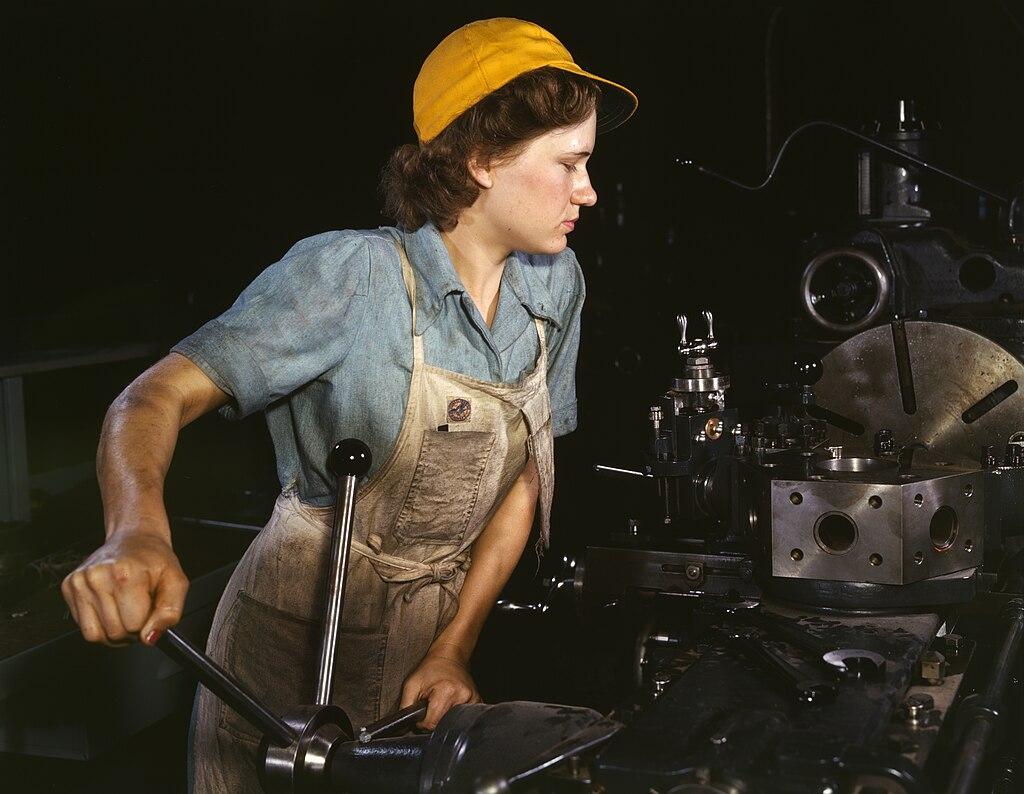
\includegraphics[width=0.45\textwidth]{chapters/chp3_pics/Factory.jpg}
\caption{\textit{Manufacturing is the foremost application of optimization in our day-to-day lives. You may even have noticed what is called `Shrinkflation': goods being shrunken down with a higher price. This is due to cost optimization.}}
    \label{fig:factory}
\end{figure}

%https://commons.wikimedia.org/wiki/File:WomanFactory1940s.jpg


\subsection*{Unconstrained Optimization} \index{Unconstrained Optimization}

\noindent Optimization is a cornerstone of mathematics, embodying the search for maxima and minima—points where a function reaches its highest or lowest values. These principles permeate problems across science, engineering, and economics, where achieving efficiency or minimizing costs is a primary objective. In this lecture, we dig deeper into the concepts of extrema by clarifying them with an applied nature. As we shift toward constrained optimization, it is essential to reflect on the foundational tools of \textit{unconstrained optimization}, which underlie more intricate scenarios. \\

\noindent Recall from our earlier discussions that the key to finding extrema lies in identifying points where the behavior of a function undergoes a qualitative change. For a differentiable function \( f: \mathbb{R}^n \to \mathbb{R} \), such points—termed \textbf{critical points}—are characterized by the condition:
\[
\nabla f(\mathbf{x}) = \mathbf{0}.
\]
At these points, the gradient, which represents the direction of steepest ascent, becomes zero, signaling that the function is momentarily stationary. Yet as we learned, not all critical points correspond to maxima or minima. Some may represent \textit{saddle points}, where the function exhibits an increase in certain directions and a decrease in others. This necessitated a framework for systematically classifying critical points.

\noindent The tools we have developed for this classification are summarized below:
\begin{enumerate}
    \item \textbf{The Gradient Condition:} Critical points are identified by solving \( \nabla f(\mathbf{x}) = \mathbf{0} \). This forms the foundation for locating potential extrema.

    \item \textbf{The Second Derivative Test:} Once critical points are located, the nature of each point is determined by examining the \textbf{Hessian matrix} \( H(\mathbf{x}) \), the matrix of second partial derivatives of \( f \). For two-variable functions, the determinant of the Hessian, denoted as \( D \), provides a straightforward method for classification:
    \[
    D = f_{xx} f_{yy} - (f_{xy})^2.
    \]
    The following rules apply:
    \begin{itemize}
        \item If \( D > 0 \) and \( f_{xx} > 0 \), the point is a local minimum.
        \item If \( D > 0 \) and \( f_{xx} < 0 \), the point is a local maximum.
        \item If \( D < 0 \), the point is neither a maximum nor a minimum and is instead a saddle point.
        \item If \( D = 0 \), the test is inconclusive, requiring further analysis.
    \end{itemize}

    \item \textbf{Boundary Analysis:} For functions defined on bounded domains, extrema may occur on the boundary. This requires evaluating \( f \) along the domain's boundary in addition to examining critical points within the interior.
\end{enumerate}

\noindent Together, these tools provide a comprehensive framework for unconstrained optimization. By systematically identifying and classifying critical points and incorporating boundary conditions where necessary, we can thoroughly analyze the behavior of a function over its domain. \\

\noindent It is worth emphasizing that unconstrained optimization closely mirrors the techniques we have already mastered. The interplay between geometry and calculus is a recurring theme: the condition \( \nabla f = \mathbf{0} \) encapsulates the geometric intuition that the gradient vanishes at extrema, while the second derivative test provides a quantitative measure of curvature. This shared foundation ensures a seamless transition into more advanced topics, as the principles of unconstrained optimization naturally extend to problems involving constraints.


\exampleline
\begin{example}
A company wants to minimize the cost of manufacturing a product. The cost function is given by 
\[
f(x, y) = x^2 + y^2 - 4x - 6y + 13,
\]
where \(x\) and \(y\) represent two key factors influencing production efficiency. Determine the optimal values of \(x\) and \(y\) to achieve the minimum cost.

\begin{solution}
This is an unconstrained optimization problem because there are no restrictions on the values \(x\) and \(y\) can take. Solving this involves finding the extrema of \(f(x, y)\), which simplifies to finding the minimum.

\begin{enumerate}
    \item \textbf{Identify Critical Points:}
    \begin{itemize}
        \item Compute the gradient of \(f\):
        \[
        \nabla f = \begin{bmatrix} \frac{\partial f}{\partial x} \\ \frac{\partial f}{\partial y} \end{bmatrix} = \begin{bmatrix} 2x - 4 \\ 2y - 6 \end{bmatrix}.
        \]
        \item Set \( \nabla f = \mathbf{0} \) to find critical points:
        \[
        2x - 4 = 0 \quad \text{and} \quad 2y - 6 = 0.
        \]
        Solving these equations gives \( x = 2 \) and \( y = 3 \). Thus, the critical point is \( (2, 3) \).
    \end{itemize}

    \item \textbf{Classify the Critical Point Using the Second Derivative Test:}
    \begin{itemize}
        \item Compute the Hessian matrix \(H\):
        \[
        H = \begin{bmatrix} 
        \frac{\partial^2 f}{\partial x^2} & \frac{\partial^2 f}{\partial x \partial y} \\ 
        \frac{\partial^2 f}{\partial y \partial x} & \frac{\partial^2 f}{\partial y^2} 
        \end{bmatrix} = \begin{bmatrix} 
        2 & 0 \\ 
        0 & 2 
        \end{bmatrix}.
        \]
        \item Calculate the determinant of \(H\):
        \[
        D = \frac{\partial^2 f}{\partial x^2} \cdot \frac{\partial^2 f}{\partial y^2} - \left( \frac{\partial^2 f}{\partial x \partial y} \right)^2 = (2)(2) - (0)^2 = 4 > 0.
        \]
        \item Since \(D > 0\) and \( \frac{\partial^2 f}{\partial x^2} = 2 > 0 \), the critical point \( (2, 3) \) is a \textbf{local minimum}.
    \end{itemize}

    \item \textbf{Evaluate the Function at the Critical Point:}
    \begin{itemize}
        \item Substituting \(x = 2\) and \(y = 3\) into \(f(x, y)\):
        \[
        f(2, 3) = (2)^2 + (3)^2 - 4(2) - 6(3) + 13 = 4 + 9 - 8 - 18 + 13 = 0.
        \]
        \item The minimum cost is \(0\), achieved when \(x = 2\) and \(y = 3\).
    \end{itemize}
\end{enumerate}
\end{solution}
\end{example}
\exampleline


\noindent This simple example reinforces the utility of these methods and foreshadows their extensions to more complex scenarios.

\subsubsection*{Classical Examples of Unconstrained Optimization}

\noindent The classical examples we explore highlight the versatility of unconstrained optimization in various settings. For each, we provide a commonly optimized formula to solidify the connection to practical applications:

\begin{enumerate}
    \item \textbf{Economic Models:} 
    \begin{itemize}
        \item Profit Maximization: Optimize the profit function \( P = R - C \), where \( R \) is revenue and \( C \) is cost.
        \item Cost Minimization: Minimize \( C(q) \), where \( C \) is the cost function and \( q \) is the quantity of goods or services produced.
    \end{itemize}
    
    \item \textbf{Physics Applications:} 
    \begin{itemize}
        \item Potential Energy Minimization: Minimize \( U = \frac{1}{2}kx^2 \), the potential energy of a spring system, where \( k \) is the spring constant and \( x \) is the displacement.
        \item Kinetic Energy Optimization: Maximize \( K = \frac{1}{2}mv^2 \), where \( m \) is mass and \( v \) is velocity.
    \end{itemize}
    
    \item \textbf{Machine Learning:} 
    \begin{itemize}
        \item Loss Function Minimization: Minimize a loss function \( L(w) = \frac{1}{N} \sum_{i=1}^N (y_i - f(x_i, w))^2 \), where \( w \) is the parameter vector, \( (x_i, y_i) \) are data points, and \( f \) is the model.
    \end{itemize}
    
    \item \textbf{Geometric Optimization:} \index{Geometric Optimization}
    \begin{itemize}
        \item Volume of a Box: Maximize \( V = l \cdot w \cdot h \), where \( l \), \( w \), and \( h \) are length, width, and height.
        \item Volume of a Sphere: Maximize \( V = \frac{4}{3}\pi r^3 \), where \( r \) is the radius.
        \item Volume of a Cylinder: Maximize \( V = \pi r^2 h \), where \( r \) is the radius and \( h \) is the height.
        \item Solids of Revolution: Optimize the volume \( V = \pi \int_a^b [f(x)]^2 \, dx \), where \( f(x) \) is the curve being rotated about an axis.
    \end{itemize}
\end{enumerate}

\noindent These examples provide a foundation for solving unconstrained optimization problems across disciplines. Each formula highlights a tangible objective, whether maximizing profit, minimizing energy, training a machine learning model, or optimizing the geometry of an object. Geometric optimization, in particular, lays the groundwork for exploring practical shapes and volumes used in design and engineering.

\exampleline
\begin{example}
Find the maximum volume of a rectangular box with its base in the \(xy\)-plane and its top lying on the plane \( z = 12 - 2x - 3y \) in the first octant.

\begin{solution}
\begin{enumerate}
    \item \textbf{Formulate the Volume Function:}
    
    \begin{itemize}
        \item The base of the box lies in the \(xy\)-plane, and its top touches the plane \( z = 12 - 2x - 3y \).
        \item The dimensions of the box are \( x \), \( y \), and \( z \), where \( z \) is given by the equation of the plane.
        \item The volume of the box is:
        \[
        V = x \cdot y \cdot z = x \cdot y \cdot (12 - 2x - 3y).
        \]
        Expand this expression:
        \[
        V(x, y) = 12xy - 2x^2y - 3xy^2.
        \]
    \end{itemize}

    \item \textbf{Find the Critical Points:}
    
    \begin{itemize}
        \item Compute the partial derivatives of \( V \):
        \[
        V_x = \frac{\partial V}{\partial x} = 12y - 4xy - 3y^2,
        \]
        \[
        V_y = \frac{\partial V}{\partial y} = 12x - 2x^2 - 6xy.
        \]
        \item Set \( V_x = 0 \) and \( V_y = 0 \):
        \[
        12y - 4xy - 3y^2 = 0 \quad \text{(1)},
        \]
        \[
        12x - 2x^2 - 6xy = 0 \quad \text{(2)}.
        \]
        Factor equation (1):
        \[
        y(12 - 4x - 3y) = 0.
        \]
        Thus, \( y = 0 \) or \( 12 - 4x - 3y = 0 \), giving \( y = \frac{12 - 4x}{3} \).

        Factor equation (2):
        \[
        x(12 - 2x - 6y) = 0.
        \]
        Thus, \( x = 0 \) or \( 12 - 2x - 6y = 0 \), giving \( y = \frac{12 - 2x}{6} = 2 - \frac{x}{3} \).

        \item Solve the system of equations:
        Substituting \( y = \frac{12 - 4x}{3} \) into \( y = 2 - \frac{x}{3} \):
        \[
        \frac{12 - 4x}{3} = 2 - \frac{x}{3}.
        \]
        Multiply through by 3:
        \[
        12 - 4x = 6 - x \quad \Rightarrow \quad 3x = 6 \quad \Rightarrow \quad x = 2.
        \]
        Substitute \( x = 2 \) into \( y = 2 - \frac{x}{3} \):
        \[
        y = 2 - \frac{2}{3} = \frac{6}{3} - \frac{2}{3} = \frac{4}{3}.
        \]
    \end{itemize}

    \item \textbf{Classify the Critical Point and Find the Volume:}
    
    The critical point is \( (x, y) = (2, \frac{4}{3}) \). At this point:
    \[
    z = 12 - 2x - 3y = 12 - 2(2) - 3\left(\frac{4}{3}\right) = 12 - 4 - 4 = 4.
    \]
    The dimensions of the box are \( x = 2 \), \( y = \frac{4}{3} \), and \( z = 4 \).
    \[
    V = x \cdot y \cdot z = 2 \cdot \frac{4}{3} \cdot 4 = \frac{32}{3}.
    \]
    Since \( V = 0 \) on the boundary of the first-octant region (where \( x = 0 \), \( y = 0 \), or \( z = 0 \)) and \( V > 0 \) at the interior critical point, this critical point must yield the maximum volume.

\end{enumerate}
\end{solution}
\end{example}
\exampleline


\subsection*{Optimization with Equality Constraints} \index{Constrained Optimization}

\noindent Consider the task of optimizing a function \( f(x, y) \) subject to a constraint \( g(x, y) = c \), where \( g \) is a differentiable function that defines a curve or surface in \( \mathbb{R}^n \). This problem can be visualized as finding the highest or lowest point on the curve or surface defined by \( g(x, y) = c \), rather than across the entire plane or space. To solve this, we introduce the method of \textbf{Lagrange multipliers}. \\

\noindent To build intuition, recall that the gradient \( \nabla g(x, y) \) of the constraint function points in the direction of the steepest ascent of \( g(x, y) \). The curve \( g(x, y) = c \) represents a level set of \( g \), and at any point along this curve, \( \nabla g(x, y) \) is normal to the curve. Similarly, the gradient \( \nabla f(x, y) \) of the objective function \( f(x, y) \) indicates the direction of steepest ascent of \( f \). At an extremum of \( f \) constrained to \( g(x, y) = c \), these gradients must align, meaning \( \nabla f(x, y) \) must point in the same or opposite direction as \( \nabla g(x, y) \).

\noindent This condition is expressed mathematically as:
\[
\nabla f(x, y) = \lambda \nabla g(x, y),
\]
where \( \lambda \) is a scalar known as the \textbf{Lagrange multiplier} \index{Lagrange Multiplier}. The scalar \( \lambda \) measures how much the objective function \( f \) changes per unit increase in the constraint \( g \).

\subsubsection*{The Lagrange Condition} \index{Lagrange Condition}

\noindent To derive this condition, consider the constrained optimization problem as finding the extrema of \( f(x, y) \) on the curve \( g(x, y) = c \). We construct the \textit{Lagrangian}: \index{Lagrange Function}
\[
\mathcal{L}(x, y, \lambda) = f(x, y) - \lambda \big(g(x, y) - c\big).
\]
\noindent The term \( \lambda(g(x, y) - c) \) enforces the constraint \( g(x, y) = c \). At the extrema of \( f(x, y) \) subject to this constraint, the gradients of \( \mathcal{L} \) with respect to \( x \), \( y \), and \( \lambda \) must vanish:
\[
\frac{\partial \mathcal{L}}{\partial x} = \frac{\partial f}{\partial x} - \lambda \frac{\partial g}{\partial x} = 0, \quad
\frac{\partial \mathcal{L}}{\partial y} = \frac{\partial f}{\partial y} - \lambda \frac{\partial g}{\partial y} = 0, \quad
\frac{\partial \mathcal{L}}{\partial \lambda} = -(g(x, y) - c) = 0.
\]
\noindent These equations are equivalent to the system:
\[
\begin{aligned}
    \nabla f(x, y) - \lambda \nabla g(x, y) &= \mathbf{0}, \\
    g(x, y) &= c.
\end{aligned}
\]

\noindent The first equation ensures that \( \nabla f \) and \( \nabla g \) are parallel (aligned with \( \lambda \)), while the second equation enforces the constraint. Thus, the optimization problem reduces to solving this system of equations for \( x \), \( y \), and \( \lambda \). \\

\noindent To solve an optimization problem using Lagrange multipliers:
\begin{enumerate}
    \item Compute \( \nabla f(x, y) \) and \( \nabla g(x, y) \).
    \item Set up the system of equations:
    \[
    \nabla f(x, y) - \lambda \nabla g(x, y) = \mathbf{0}, \quad g(x, y) = c.
    \]
    \item Solve the system for \( x \), \( y \), and \( \lambda \).
    \item Evaluate \( f(x, y) \) at the solutions to determine the extrema.
\end{enumerate}

\noindent The equation \( \nabla f = \lambda \nabla g \) has a powerful geometric interpretation. Recall that \( \nabla g(x, y) \) is orthogonal to the level curve \( g(x, y) = c \) at any point. Similarly, \( \nabla f(x, y) \) is orthogonal to the level curve of \( f(x, y) \). Thus, the condition \( \nabla f = \lambda \nabla g \) implies that the level curves of \( f \) and \( g \) are tangent at the optimal point. This tangency ensures that \( f(x, y) \) is extremized subject to the constraint \( g(x, y) = c \).

\exampleline
\begin{example}
Find the minimum of the function \( f(x, y) = x^2 + y^2 \) subject to the constraint \( x + y = 2 \).

\begin{solution}
\begin{enumerate}
    \item \textbf{Formulate the Lagrangian:}
    
    To apply the method of Lagrange multipliers, we introduce a Lagrange multiplier \( \lambda \) and construct the Lagrangian function:
    \[
    \mathcal{L}(x, y, \lambda) = f(x, y) - \lambda (g(x, y) - c),
    \]
    where \( g(x, y) = x + y \) and \( c = 2 \).
    
    Substituting the given functions:
    \[
    \mathcal{L}(x, y, \lambda) = x^2 + y^2 - \lambda (x + y - 2).
    \]
    
    \item \textbf{Compute the Partial Derivatives:}
    
    To find the extrema, take the partial derivatives of \( \mathcal{L} \) with respect to \( x \), \( y \), and \( \lambda \), and set them equal to zero.
    
    \begin{itemize}
        \item \textbf{Partial derivative with respect to \( x \):}
        \[
        \frac{\partial \mathcal{L}}{\partial x} = 2x - \lambda = 0 \quad \Rightarrow \quad \lambda = 2x \quad (1)
        \]
        
        \item \textbf{Partial derivative with respect to \( y \):}
        \[
        \frac{\partial \mathcal{L}}{\partial y} = 2y - \lambda = 0 \quad \Rightarrow \quad \lambda = 2y \quad (2)
        \]
        
        \item \textbf{Partial derivative with respect to \( \lambda \):}
        \[
        \frac{\partial \mathcal{L}}{\partial \lambda} = -(x + y - 2) = 0 \quad \Rightarrow \quad x + y = 2 \quad (3)
        \]
    \end{itemize}
    
    \item \textbf{Solve the System of Equations:}
    
    From equations (1) and (2):
    \[
    2x = \lambda \quad \text{and} \quad 2y = \lambda \quad \Rightarrow \quad 2x = 2y \quad \Rightarrow \quad x = y
    \]
    
    Substitute \( x = y \) into equation (3):
    \[
    x + x = 2 \quad \Rightarrow \quad 2x = 2 \quad \Rightarrow \quad x = 1
    \]
    
    Since \( x = y \):
    \[
    y = 1
    \]
    
    Thus, the critical point is \( (x, y) = (1, 1) \).
    
    \item \textbf{Verify the Solution:}
    
    Substitute \( x = 1 \) and \( y = 1 \) back into the objective function:
    \[
    f(1, 1) = (1)^2 + (1)^2 = 1 + 1 = 2
    \]
    
    Therefore, the function \( f(x, y) = x^2 + y^2 \) attains its minimum value of 2 at the point \( (1, 1) \) under the constraint \( x + y = 2 \).
    
    \item \textbf{Visualization:}
    
    To better understand the optimization, let's visualize the objective function, the constraint, and the optimal point.
    
    \begin{figure}[H]
        \centering
        \begin{tikzpicture}
            \begin{axis}[
                xlabel={$x$},
                ylabel={$y$},
                axis lines=middle,
                grid=both,
                minor grid style={gray!25},
                major grid style={gray!50},
                legend pos=outer north east,
                width=12cm,
                height=12cm,
                samples=100, % Increased samples for smoother circles
                domain=0:360, % Angle domain in degrees
                xmin=-1, xmax=3,
                ymin=-1, ymax=3,
                xtick={-1,0,1,2,3},
                ytick={-1,0,1,2,3},
            ]
                % Contour lines for f(x,y) = x^2 + y^2
                \foreach \r in {1,2,4,6,8,10} {
                    \addplot [
                        blue,
                        thick,
                        forget plot % Prevents each contour line from adding to the legend
                    ] 
                        ({sqrt(\r)*cos(\x)}, {sqrt(\r)*sin(\x)});
                }
                % Manually add a single legend entry for the contour lines
                \addlegendimage{blue, thick}
                \addlegendentry{$f(x, y) = x^2 + y^2$}
                
                % Constraint line x + y = 2
                \addplot [
                    red,
                    thick,
                    domain=0:2,
                    samples=2
                ]
                {2 - x};
                \addlegendentry{Constraint $x + y = 2$}
                
                % Optimal point (1,1)
                \addplot[
                    only marks,
                    mark=*,
                    mark size=3pt,
                    black
                ] coordinates {(1,1)};
                \addlegendentry{Optimal Point $(1, 1)$}
                
                % Gradient of f: ∇f = [2x, 2y] at (1,1) => [2,2]
                \addplot[
                    ->,
                    very thick,
                    green,
                    >=stealth
                ] coordinates {(1,1) (1+2*0.5,1+2*0.5)}; % Scaled for visibility
                \addlegendentry{$\nabla f = (2, 2)$}
                
                % Gradient of g: ∇g = [1, 1] at (1,1)
                \addplot[
                    ->,
                    very thick,
                    orange,
                    >=stealth
                ] coordinates {(1,1) (1+1*0.5,1+1*0.5)}; % Scaled for visibility
                \addlegendentry{$\nabla g = (1, 1)$}
                
                % Annotation for the optimal point
                \node at (axis cs:1.2,.8) [anchor=south west] {$(1, 1)$};
            \end{axis}
        \end{tikzpicture}
        \caption{\textit{Visualization of the optimization problem using Lagrange multipliers. The blue circles represent the contour lines of the objective function \( f(x, y) = x^2 + y^2 \), the red line is the constraint \( x + y = 2 \), the black dot marks the optimal point \( (1, 1) \), the green arrow represents the gradient \( \nabla f \), and the orange arrow represents the gradient \( \nabla g \).}}
        \label{fig:lagrange_multiplier_plot_example}
    \end{figure}
    
\end{enumerate}
\end{solution}
\end{example}

\exampleline


\noindent Let's now try a problem that's a little messier and doesn't have a nice answer. We will need to use a computer to solve a polynomial using numerical approximation at the end. This is more representative of a problem you may encounter in an actual professional setting.


\exampleline
\begin{example} Determine the production levels \( x \) and \( y \) for Gadget A and Gadget B, respectively, that minimize the total production cost given by:
\[
C(x, y) = x^2 y + y^3,
\]
subject to the nonlinear constraint:
\[
x^3 + y^3 = 2000.
\]
Since production levels must be integer values, round the approximate solution up or down and choose the option with the lesser cost.

\begin{solution}
\begin{enumerate}
    \item \textbf{Formulate the Lagrangian:}
    
    Introduce a Lagrange multiplier \( \lambda \) and construct the Lagrangian function:
    \[
    \mathcal{L}(x, y, \lambda) = C(x, y) - \lambda (x^3 + y^3 - 2000).
    \]
    Substituting the given functions:
    \[
    \mathcal{L}(x, y, \lambda) = x^2 y + y^3 - \lambda (x^3 + y^3 - 2000).
    \]
    
    \item \textbf{Compute the Partial Derivatives:}
    
    To find the extrema, take the partial derivatives of \( \mathcal{L} \) with respect to \( x \), \( y \), and \( \lambda \), and set them equal to zero.
    
    \begin{itemize}
        \item \textbf{Partial derivative with respect to \( x \):}
        \[
        \frac{\partial \mathcal{L}}{\partial x} = 2xy - 3\lambda x^2 = 0 \quad \Rightarrow \quad 2xy = 3\lambda x^2 \quad (1)
        \]
        
        \item \textbf{Partial derivative with respect to \( y \):}
        \[
        \frac{\partial \mathcal{L}}{\partial y} = x^2 + 3y^2 - 3\lambda y^2 = 0 \quad \Rightarrow \quad x^2 + 3y^2 = 3\lambda y^2 \quad (2)
        \]
        
        \item \textbf{Partial derivative with respect to \( \lambda \):}
        \[
        \frac{\partial \mathcal{L}}{\partial \lambda} = -(x^3 + y^3 - 2000) = 0 \quad \Rightarrow \quad x^3 + y^3 = 2000 \quad (3)
        \]
    \end{itemize}
    
    \item \textbf{Solve the System of Equations:}
    
    From equation (1):
    \[
    2xy = 3\lambda x^2 \quad \Rightarrow \quad \lambda = \frac{2y}{3x} \quad (1a)
    \]
    
    From equation (2):
    \[
    x^2 + 3y^2 = 3\lambda y^2 \quad \Rightarrow \quad \lambda = \frac{x^2 + 3y^2}{3y^2} = \frac{x^2}{3y^2} + 1 \quad (2a)
    \]
    
    Equate the two expressions for \( \lambda \):
    \[
    \frac{2y}{3x} = \frac{x^2}{3y^2} + 1
    \]
    
    Multiply both sides by \( 3x y^2 \) to eliminate denominators:
    \[
    2y \cdot y^2 = x^3 + 3x y^2
    \]
    \[
    2y^3 = x^3 + 3x y^2 \quad (4)
    \]
    
    From the constraint (3):
    \[
    x^3 + y^3 = 2000 \quad \Rightarrow \quad x^3 = 2000 - y^3 \quad (5)
    \]
    
    Substitute \( x^3 = 2000 - y^3 \) into equation (4):
    \[
    2y^3 = (2000 - y^3) + 3x y^2
    \]
    \[
    2y^3 = 2000 - y^3 + 3x y^2
    \]
    \[
    3x y^2 = 3y^3 - 2000
    \]
    \[
    x y^2 = y^3 - \frac{2000}{3} \quad (6)
    \]
    
    Solve for \( x \):
    \[
    x = \frac{y^3 - \frac{2000}{3}}{y^2} = y - \frac{2000}{3y^2} \quad (7)
    \]
    
    Substitute \( x = y - \frac{2000}{3y^2} \) into the constraint \( x^3 + y^3 = 2000 \):
    \[
    \left(y - \frac{2000}{3y^2}\right)^3 + y^3 = 2000
    \]
    
    This equation is highly complex and does not yield to simple algebraic methods. Therefore, we proceed with an approximate numerical solution. For more detailed computations, refer to the \href{https://www.wolframalpha.com/widgets/view.jsp?id=1451afdfe5a25b2a316377c1cd488883}{Wolfram Alpha Lagrange Multipliers} tool.
    
    \item \textbf{Approximate Solution:}
    
    The approximate solution is:
    \[
    (x, y) \approx (7.04423, 11.8177)
    \]
    
    \item \textbf{Decision on Integer Production Levels:}
    
    Since production levels must be integer values, we consider the nearest integer values to the approximate solution. The four possible combinations are:

    \begin{itemize}
        \item Option 1: \( x = 7 \), \( y = 11 \)
        \[
        x^3 + y^3 = 343 + 1331 = 1674 \leq 2000 \quad (\text{Satisfies the constraint})
        \]
        
        \item Option 2: \( x = 7 \), \( y = 12 \)
        \[
        x^3 + y^3 = 343 + 1728 = 2071 > 2000 \quad (\text{Does not satisfy the constraint})
        \]
        
        \item Option 3: \( x = 8 \), \( y = 11 \)
        \[
        x^3 + y^3 = 512 + 1331 = 1843 \leq 2000 \quad (\text{Satisfies the constraint})
        \]
        
        \item Option 4: \( x = 8 \), \( y = 12 \)
        \[
        x^3 + y^3 = 512 + 1728 = 2240 > 2000 \quad (\text{Does not satisfy the constraint})
        \]
    \end{itemize}
    
    Therefore, only Option 1 and Option 3 satisfy the constraint.
    
    \textbf{Compute the Total Cost for Each Option:}
    \begin{itemize}
        \item Option 1: \( x = 7 \), \( y = 11 \)
        \[
        C(7, 11) = 7^2 \times 11 + 11^3 = 49 \times 11 + 1331 = 539 + 1331 = 1870
        \]
        
        \item Option 3: \( x = 8 \), \( y = 11 \)
        \[
        C(8, 11) = 8^2 \times 11 + 11^3 = 64 \times 11 + 1331 = 704 + 1331 = 2035
        \]
    \end{itemize}
    
    \textbf{Decision:}  
    Choose the production levels that satisfy the constraint and incur the lesser cost. Between Option 1 and Option 3:
    \[
    1870 < 2035
    \]
    
    Therefore, Option 1 (\( x = 7 \), \( y = 11 \)) is the optimal integer production level with a total cost of \$1,870.
    
    \item \textbf{Visualization:}
    
    To better understand the optimization, let's visualize the nonlinear constraint, the approximate optimal point, the integer production options, and their associated costs.
    

\begin{figure}[H]
    \centering
    \begin{tikzpicture}
        \begin{axis}[
            xlabel={$x$},
            ylabel={$y$},
            axis lines=middle,
            grid=both,
            minor grid style={gray!25},
            major grid style={gray!50},
            legend style={
                font=\small, 
                at={(1.05,1)}, 
                anchor=north west
            },
            width=12cm,
            height=12cm,
            ymin=8, ymax=14.4, % Adjusted to accommodate y=16.46
            xmin=6, xmax=12.4, % Adjusted to accommodate x=16.46
            xtick={0,2,4,6,8,10},
            ytick={0,2,4,6,8,10,12,14},
        ]
            % Precomputed Level Curve C=2237.10
            \addplot [
                black!50,
                thick,
                smooth,
            ]
                coordinates {
                    (16.46,7)
                    (15.56,7.5)
                    (14.69,8)
                    (13.81,8.5)
                    (12.95,9)
                    (12.05,9.5)
                    (11.12,10)
                    (10.11,10.5)
                    (9.07,11)
                    (7.89,11.5)
                    (7.04,11.82)
                    (6.52,12)
                };
            \addlegendentry{Level Curve of $C$}

            % Nonlinear constraint x^3 + y^3 = 2000
            \addplot [
                red,
                thick,
                domain=6:12, % Adjusted domain to avoid complex numbers
                samples=200,
            ]
                { (2000 - x^3)^(1/3) };
            \addlegendentry{Constraint}

            % Chosen Option: (7.04, 11.82) as a star
            \addplot[
                mark=star,
                mark size=6pt,
                color=blue,
                only marks,
            ] coordinates {(7.04,11.82)};
            \addlegendentry{True Solution}

            % Integer Option 1: (7,11) - Blue Circle (Inside Constraint)
            \addplot[
                only marks,
                mark=*,
                mark size=4pt,
                blue
            ] coordinates {(7,11)};
            \addlegendentry{Option 1}

            % Integer Option 2: (7,12) - Red Circle (Outside Constraint)
            \addplot[
                only marks,
                mark=*,
                mark size=4pt,
                red
            ] coordinates {(7,12)};
            \addlegendentry{Option 2}

            % Integer Option 3: (8,11) - Blue Circle (Inside Constraint)
            \addplot[
                only marks,
                mark=*,
                mark size=4pt,
                blue
            ] coordinates {(8,11)};
            \addlegendentry{Option 3}

            % Integer Option 4: (8,12) - Red Circle (Outside Constraint)
            \addplot[
                only marks,
                mark=*,
                mark size=4pt,
                red
            ] coordinates {(8,12)};
            \addlegendentry{Option 4}

            % Gradient of C: ∇C = [2xy, x^2 + 3y^2] at (7.04,11.82) ≈ [166.52, 469.14]
            % Scaled down by factor 0.005 for visibility
            \addplot[
                ->,
                very thick,
                orange,
                >=stealth
            ] coordinates {
                (7.04,11.82) 
                (7.04 + 166.52*0.005, 11.82 + 469.14*0.005)
            };
            \addlegendentry{$\nabla C$}

            % Gradient of g: ∇g = [3x^2, 3y^2] at (7.04,11.82) ≈ [147.42, 420.0]
            % Scaled down by factor 0.005 for visibility
            \addplot[
                ->,
                very thick,
                purple,
                >=stealth
            ] coordinates {
                (7.04,11.82) 
                (7.04 + 147.42*0.005, 11.82 + 420.0*0.005)
            };
            \addlegendentry{$\nabla g$}

            % Annotations for points
            \node at (axis cs:7.3,11.5) [anchor=south west] {$(7.04, 11.82)$};
            \node at (axis cs:7,11) [anchor=north east] {$(7, 11)$};
            \node at (axis cs:7,12) [anchor=south east] {$(7, 12)$};
            \node at (axis cs:8,11) [anchor=north west] {$(8, 11)$};
            \node at (axis cs:8,12) [anchor=south west] {$(8, 12)$};
        \end{axis}
    \end{tikzpicture}
    \caption{\textit{Visualization of the optimization problem with nonlinear constraint. Red curve: \( x^3 + y^3 = 2000 \). Blue star: Chosen Option \( (7.04, 11.82) \). Blue circles: Options 1 \& 3 (Inside Constraint). Red circles: Options 2 \& 4 (Outside Constraint). Orange arrow: \( \nabla C \). Purple arrow: \( \nabla g \). Level Curve: \( C(x, y) = 2237.10 \).}}
    \label{fig:lagrange_multiplier_complex_example}
\end{figure}


\end{enumerate}
\end{solution}
\end{example}
\exampleline


\subsubsection*{Optimization with Multiple Equality Constraints} \index{Constrained Optimization}

\noindent When optimizing a function \( f(x, y, z) \) subject to two or more equality constraints, such as \( g(x, y, z) = c_1 \) and \( h(x, y, z) = c_2 \), the method of Lagrange multipliers naturally extends to accommodate additional constraints. The underlying principle remains the same: at an optimal point, the gradients of \( f \), \( g \), and \( h \) must align in such a way that any movement satisfying the constraints does not produce a first-order change in \( f \).

\noindent For two constraints, we define the \textit{Lagrangian} as:
\[
\mathcal{L}(x, y, z, \lambda_1, \lambda_2) = f(x, y, z) - \lambda_1 \big(g(x, y, z) - c_1\big) - \lambda_2 \big(h(x, y, z) - c_2\big).
\]
\noindent The gradients of \( \mathcal{L} \) with respect to all variables must vanish at the extrema, leading to the system of equations:
\[
\begin{aligned}
    \nabla f(x, y, z) - \lambda_1 \nabla g(x, y, z) - \lambda_2 \nabla h(x, y, z) &= \mathbf{0}, \\
    g(x, y, z) &= c_1, \\
    h(x, y, z) &= c_2.
\end{aligned}
\]

\noindent In practice:
\begin{enumerate}
    \item Compute \( \nabla f(x, y, z) \), \( \nabla g(x, y, z) \), and \( \nabla h(x, y, z) \).
    \item Solve the system of equations for \( x, y, z, \lambda_1, \) and \( \lambda_2 \).
    \item Evaluate \( f(x, y, z) \) at the solutions to determine the extrema.
\end{enumerate}

\subsubsection*{Generalization to \( n \) Equality Constraints}

\noindent For a general optimization problem with \( n \) variables and \( m \) equality constraints:
\[
\begin{aligned}
    \text{Minimize (or maximize):} & \quad f(x_1, x_2, \dots, x_n), \\
    \text{Subject to:} & \quad g_1(x_1, x_2, \dots, x_n) = c_1, \\
    & \quad g_2(x_1, x_2, \dots, x_n) = c_2, \\
    & \quad \dots, \\
    & \quad g_m(x_1, x_2, \dots, x_n) = c_m,
\end{aligned}
\]
the Lagrange function is defined as:
\[
\mathcal{L}(x_1, x_2, \dots, x_n, \lambda_1, \lambda_2, \dots, \lambda_m) = f(x_1, x_2, \dots, x_n) - \sum_{i=1}^m \lambda_i \big(g_i(x_1, x_2, \dots, x_n) - c_i\big).
\]

\noindent The necessary conditions for an extremum are:
\[
\begin{aligned}
    \nabla f(x_1, x_2, \dots, x_n) - \sum_{i=1}^m \lambda_i \nabla g_i(x_1, x_2, \dots, x_n) &= \mathbf{0}, \\
    g_1(x_1, x_2, \dots, x_n) &= c_1, \\
    g_2(x_1, x_2, \dots, x_n) &= c_2, \\
    & \quad \dots, \\
    g_m(x_1, x_2, \dots, x_n) &= c_m.
\end{aligned}
\]

\noindent In the general case, the gradients \( \nabla g_1, \nabla g_2, \dots, \nabla g_m \) define a space of feasible directions, and the gradient \( \nabla f \) must align with this space at the extremum. Specifically, \( \nabla f \) must lie in the span of \( \nabla g_1, \nabla g_2, \dots, \nabla g_m \), reflecting the fact that movement within the feasible region does not change \( f \) to first order.


\exampleline
\begin{example}
A nutritionist wants to find the optimal levels \( x \) and \( y \) (in grams) of two ingredients to minimize a certain dietary risk function. Suppose the overall risk is modeled by:
\[
f(x,y) = x^2 + xy + 2y^2.
\]
They must satisfy two nutritional constraints to ensure dietary balance:
\[
x + 2y = 10, \quad \text{and} \quad x - y = 3.
\]

\begin{solution}
\begin{enumerate}
    \item \textbf{Set up the Lagrangian:} Introduce Lagrange multipliers \(\lambda\) and \(\mu\) for the two constraints:
    \[
    \mathcal{L}(x,y,\lambda,\mu) = x^2 + xy + 2y^2 - \lambda(x + 2y - 10) - \mu(x - y - 3).
    \]

    \item \textbf{Compute Partial Derivatives:} Take partial derivatives and set them equal to zero.
    \[
    \frac{\partial \mathcal{L}}{\partial x} = 2x + y - \lambda - \mu = 0,
    \]
    \[
    \frac{\partial \mathcal{L}}{\partial y} = x + 4y - 2\lambda + \mu = 0,
    \]
    \[
    \frac{\partial \mathcal{L}}{\partial \lambda} = -(x + 2y - 10) = 0,
    \]
    \[
    \frac{\partial \mathcal{L}}{\partial \mu} = -(x - y - 3) = 0.
    \]

    \item \textbf{From the Constraints:} 
    \[
    x + 2y = 10, \quad x - y = 3.
    \]
    Solve these directly first:
    From \(x - y = 3\), we get \(x = 3 + y\).
    Substitute into \(x + 2y = 10\):
    \[
    (3 + y) + 2y = 10 \implies 3 + 3y = 10 \implies 3y = 7 \implies y = \tfrac{7}{3}.
    \]
    Thus, \(x = 3 + \tfrac{7}{3} = \tfrac{16}{3}\).

    \item \textbf{Check Optimality:}
    Substitute \((x,y)=\left(\tfrac{16}{3}, \tfrac{7}{3}\right)\) into the objective:
    \[
    f\left(\tfrac{16}{3}, \tfrac{7}{3}\right) = \left(\tfrac{16}{3}\right)^2 + \left(\tfrac{16}{3}\cdot\tfrac{7}{3}\right) + 2\left(\tfrac{7}{3}\right)^2.
    \]
    Compute:
    \[
    \left(\tfrac{16}{3}\right)^2 = \tfrac{256}{9}, \quad \tfrac{16}{3}\cdot \tfrac{7}{3}=\tfrac{112}{9}, \quad 2\left(\tfrac{7}{3}\right)^2 = 2\left(\tfrac{49}{9}\right)=\tfrac{98}{9}.
    \]
    Sum them up:
    \[
    f\left(\tfrac{16}{3}, \tfrac{7}{3}\right) = \tfrac{256}{9} + \tfrac{112}{9} + \tfrac{98}{9} = \tfrac{466}{9}.
    \]

    The point \(\left(\tfrac{16}{3}, \tfrac{7}{3}\right)\) satisfies both constraints and yields the minimized risk value \(\frac{466}{9}\).

\end{enumerate}
\end{solution}
\end{example}
\exampleline


\subsection*{Optimization with Inequality Constraints} \index{Optimization with Inequality Constraints}

\noindent So far we have used Lagrange multipliers to handle constraints of the form $g(\mathbf{x}) = c$. But many real problems involve \textit{inequality} constraints --- a budget that may not be exceeded, a quota that must be met, a physical quantity that cannot be negative. The \textbf{Karush--Kuhn--Tucker (KKT) conditions} \index{Karush-Kuhn-Tucker Conditions} extend the Lagrange machinery to this setting.

\noindent Consider the general problem
\[
\text{minimize } f(\mathbf{x}) \qquad \text{subject to } g_i(\mathbf{x}) \geq 0, \quad i = 1, \ldots, m.
\]
Form the Lagrangian
\[
\mathcal{L}(\mathbf{x}, \boldsymbol{\mu}) \;=\; f(\mathbf{x}) - \sum_{i=1}^{m} \mu_i \, g_i(\mathbf{x}).
\]
At an optimum $\mathbf{x}^*$ there exist multipliers $\mu_1^*, \ldots, \mu_m^*$ satisfying the four \textbf{KKT conditions}:

\begin{center}
\renewcommand{\arraystretch}{1.5}
\begin{tabular}{@{}p{0.32\textwidth}p{0.34\textwidth}p{0.28\textwidth}@{}}
\toprule
\textbf{Condition} & \textbf{Statement} & \textbf{Meaning} \\
\midrule
1. Stationarity & $\nabla f(\mathbf{x}^*) = \displaystyle\sum_{i=1}^{m} \mu_i^* \, \nabla g_i(\mathbf{x}^*)$ & $\nabla \mathcal{L} = \mathbf{0}$ at $\mathbf{x}^*$ \\
2. Primal feasibility & $g_i(\mathbf{x}^*) \geq 0$ for all $i$ & the answer is in the feasible set \\
3. Dual feasibility & $\mu_i^* \geq 0$ for all $i$ & multipliers cannot pull the wrong way \\
4. Complementary slackness & $\mu_i^* \, g_i(\mathbf{x}^*) = 0$ for all $i$ & each constraint is either active or inert \\
\bottomrule
\end{tabular}
\end{center}

\noindent The fourth condition is the engine of KKT. For each constraint $i$, exactly one of the following holds:
\begin{itemize}\setlength{\itemsep}{2pt}
  \item $g_i(\mathbf{x}^*) = 0$ \;---\; the constraint is \emph{active} (binding) and the multiplier $\mu_i^*$ is allowed to be positive, or
  \item $g_i(\mathbf{x}^*) > 0$ \;---\; the constraint is \emph{inactive} (slack) and $\mu_i^* = 0$ is forced.
\end{itemize}
A constraint that is not binding contributes nothing to stationarity --- the machinery automatically ignores it. This is precisely how the KKT system selects which constraints actually shape the optimum.

\subsubsection*{Connection to Lagrange Multipliers}

\noindent Equality constraints are the special case in which every constraint is forced to be active. If we have $h_j(\mathbf{x}) = 0$, then primal feasibility forces $h_j = 0$ automatically, complementary slackness becomes vacuous, and the multiplier sign restriction disappears (the multiplier $\lambda_j$ may take any sign). What remains of the KKT system is exactly $\nabla f = \sum_j \lambda_j \nabla h_j$ --- the Lagrange condition. So KKT is not a different theory; it is the natural generalization that allows constraints to be inequalities, with complementary slackness deciding which ones bind.

\subsubsection*{Solving by Case Analysis}

\noindent For a problem with $m$ inequality constraints, complementary slackness divides the analysis into up to $2^m$ cases (each constraint is active or inactive). For small $m$ we can enumerate them: assume a particular subset is active, solve the resulting equations from stationarity together with the active equalities, then discard any case that violates primal feasibility ($g_i < 0$) or dual feasibility ($\mu_i < 0$). The surviving candidates are compared, and the smallest value of $f$ wins. For large $m$ specialized algorithms (interior-point, active-set, sequential minimal optimization) take over, but the underlying conditions are the same four equations above.

\subsubsection*{Applications to Machine Learning}

\noindent In machine learning, constraints can help guide the training of models in practical ways. For example, suppose you want to train a model that makes predictions under limited computational resources. You might enforce an inequality constraint that keeps the model complexity below a certain threshold. Or perhaps you need to ensure fairness, such as enforcing that the model’s error rate for one demographic group does not exceed its error rate for another group by more than a certain amount. These kinds of constraints lead to inequality conditions that can be analyzed using the KKT framework. The underlying principle remains the same: find model parameters that minimize a loss function while respecting the given inequalities.

\exampleline
\begin{example}
\noindent \textbf{(Support Vector Machine --- a classification problem from machine learning.)} A \textit{Support Vector Machine} (SVM) \index{Support Vector Machines} finds a separating line $\mathbf{w}\cdot\mathbf{x} + b = 0$ between two classes of data with the widest possible \textit{margin}. Geometrically, the parallel lines $\mathbf{w}\cdot\mathbf{x} + b = +1$ and $\mathbf{w}\cdot\mathbf{x} + b = -1$ skim the closest points of each class; the gap between them is $\dfrac{2}{\|\mathbf{w}\|}$. Maximizing the margin is therefore equivalent to minimizing $\tfrac{1}{2}\|\mathbf{w}\|^2$, subject to every point being on the correct side: $y_i(\mathbf{w}\cdot\mathbf{x}_i + b) \geq 1$.

\noindent Consider three labeled points in $\mathbb{R}^2$:
\[
\mathbf{x}_1 = (1,1), \;\; y_1 = +1; \qquad \mathbf{x}_2 = (-1,-1), \;\; y_2 = -1; \qquad \mathbf{x}_3 = (3,3), \;\; y_3 = +1.
\]
Find the maximum-margin classifier $\mathbf{w} = (w_1, w_2)$, $b$ by solving
\[
\text{minimize } \tfrac{1}{2}(w_1^2 + w_2^2) \qquad \text{subject to } \quad y_i\bigl(w_1 x_{i,1} + w_2 x_{i,2} + b\bigr) - 1 \geq 0, \;\; i = 1,2,3.
\]

\begin{solution}
\noindent Writing out the three inequality constraints:
\[
g_1 = w_1 + w_2 + b - 1 \geq 0, \qquad g_2 = w_1 + w_2 - b - 1 \geq 0, \qquad g_3 = 3w_1 + 3w_2 + b - 1 \geq 0.
\]

\noindent\textbf{Step 1: Stationarity.} The KKT condition $\nabla f = \mu_1 \nabla g_1 + \mu_2 \nabla g_2 + \mu_3 \nabla g_3$, taken component-wise in $(w_1, w_2, b)$, gives
\[
w_1 = \mu_1 + \mu_2 + 3\mu_3, \qquad w_2 = \mu_1 + \mu_2 + 3\mu_3, \qquad 0 = \mu_1 - \mu_2 + \mu_3.
\]
The first two equations force $w_1 = w_2$; call the common value $w$.

\noindent\textbf{Step 2: Pick the active set.} The geometry suggests $\mathbf{x}_3 = (3,3)$ sits well inside the $+1$ region while $\mathbf{x}_1$ and $\mathbf{x}_2$ are the closest pair. Try \textit{constraints 1 and 2 active, constraint 3 inactive} ($\mu_3 = 0$).

Active equations $g_1 = g_2 = 0$:
\[
2w + b = 1, \qquad 2w - b = 1 \quad \Longrightarrow \quad w = \tfrac{1}{2}, \;\; b = 0.
\]
With $\mu_3 = 0$ and $w = \tfrac{1}{2}$, stationarity reduces to $\tfrac{1}{2} = \mu_1 + \mu_2$ and $\mu_1 = \mu_2$, so
\[
\mu_1 = \mu_2 = \tfrac{1}{4}, \qquad \mu_3 = 0.
\]

\noindent\textbf{Step 3: Verify all four KKT conditions.}
\begin{itemize}\setlength{\itemsep}{2pt}
  \item \textbf{Stationarity:} $w_1 = w_2 = \tfrac{1}{4} + \tfrac{1}{4} + 3(0) = \tfrac{1}{2}$ \checkmark; \;\; $\mu_1 - \mu_2 + \mu_3 = 0$ \checkmark.
  \item \textbf{Primal feasibility:} $g_1 = g_2 = 0 \geq 0$ \checkmark; \;\; $g_3 = \tfrac{3}{2} + \tfrac{3}{2} + 0 - 1 = 2 \geq 0$ \checkmark.
  \item \textbf{Dual feasibility:} $\mu_1 = \mu_2 = \tfrac{1}{4} \geq 0$, $\mu_3 = 0 \geq 0$ \checkmark.
  \item \textbf{Complementary slackness:} $\mu_1 g_1 = \tfrac{1}{4}\cdot 0 = 0$ \checkmark; \;\; $\mu_2 g_2 = 0$ \checkmark; \;\; $\mu_3 g_3 = 0\cdot 2 = 0$ \checkmark.
\end{itemize}
All four conditions hold. Because $f$ is strictly convex and the feasible region (intersection of half-planes) is convex, this KKT point is the unique global minimum.

\noindent\textbf{Step 4: Read off the answer.}
\[
\boxed{\;\mathbf{w}^* = \bigl(\tfrac{1}{2},\,\tfrac{1}{2}\bigr), \quad b^* = 0, \quad \tfrac{1}{2}\|\mathbf{w}^*\|^2 = \tfrac{1}{4}, \quad \text{margin} = \tfrac{2}{\|\mathbf{w}^*\|} = 2\sqrt{2}.\;}
\]
The decision boundary is $\tfrac{1}{2}x_1 + \tfrac{1}{2}x_2 = 0$, i.e. the line $x_1 + x_2 = 0$.

\noindent\textbf{Interpretation.} The two points $\mathbf{x}_1 = (1,1)$ and $\mathbf{x}_2 = (-1,-1)$ lie exactly on the margin lines and have $\mu_1, \mu_2 > 0$: they are the \textit{support vectors}, the data points that determine the classifier. The third point $\mathbf{x}_3 = (3,3)$ is well inside the $+1$ region, so $g_3 > 0$ and complementary slackness forces $\mu_3 = 0$ --- it contributes nothing and could be removed without changing the answer. This is the geometric content of the KKT conditions in SVM: the optimum is built only from the binding constraints.
\end{solution}
\end{example}
\exampleline

\noindent The SVM example illustrates the general lesson: when an optimum lies inside the feasible region, the corresponding inequality constraint sleeps and its multiplier is zero; only the constraints that the optimum actually touches enter the stationarity equation. This selection mechanism is what makes the KKT framework, despite its apparent complexity, both algorithmically tractable and geometrically transparent.















\newpage

\formsdefs{}

\subsection*{Important Vocabulary}
\begin{itemize}
    \item \textbf{Function of Two Variables:} A rule that assigns a real number \( z = f(x, y) \) to each ordered pair \( (x, y) \) in a subset of \( \mathbb{R}^2 \). The graph is a surface in \( \mathbb{R}^3 \).
    \item \textbf{Domain:} The set of all input pairs \( (x, y) \) where the function \( f(x, y) \) is defined.
    \item \textbf{Range:} The set of all output values \( z \) produced by \( f(x, y) \).
    \item \textbf{Level Curves:} Curves in the \( xy \)-plane where \( f(x, y) = k \) for constant \( k \).
    \item \textbf{Cross-Sections:} Slices of the surface \( z = f(x, y) \) obtained by fixing one variable \( x \) or \( y \).
    \item \textbf{Level Surfaces:} Surfaces in \( \mathbb{R}^3 \) where \( f(x, y, z) = k \) for constant \( k \).
    \item \textbf{Limit:} For a function \( f(x, y) \), the limit at \( (a, b) \) is the value \( L \) such that \( f(x, y) \) approaches \( L \) as \( (x, y) \to (a, b) \) from any direction.
    \item \textbf{Path Dependence:} A limit does not exist if the value of \( f(x, y) \) depends on the path taken to approach \( (a, b) \).
    \item \textbf{Continuity:} \( f(x, y) \) is continuous at \( (a, b) \) if:
    \[
    \lim_{(x, y) \to (a, b)} f(x, y) = f(a, b).
    \]
    \item \textbf{Partial Derivative:} The derivative of a multivariable function with respect to one variable, holding all others constant.
    \item \textbf{Clairaut's Theorem:} States that mixed partial derivatives are equal when certain continuity conditions are met.
    \item \textbf{Implicit Differentiation:} A technique for finding derivatives when relationships between variables are defined implicitly.
    \item \textbf{Directional Derivative:} The rate of change of a function in a specific direction, quantified using a unit vector.
    \item \textbf{Gradient Vector:} A vector field containing all partial derivatives, pointing in direction of steepest increase.
    \item \textbf{Tangent Plane:} A plane that touches a surface at a point and provides the best linear approximation near that point.
    \item \textbf{Differentials:} Small increments in variables used to approximate changes in functions.
    \item \textbf{Critical Point:} A point where all partial derivatives are zero or at least one does not exist.
    \item \textbf{Local Maximum/Minimum:} A point where function value is higher/lower than all nearby points.
    \item \textbf{Global Maximum/Minimum:} A point where function value is highest/lowest over entire domain.
    \item \textbf{Saddle Point:} A critical point that is neither a maximum nor minimum.
    \item \textbf{Hessian Matrix:} Matrix of all second partial derivatives of a function.
    \item \textbf{Discriminant:} Determinant of the Hessian matrix in two dimensions.
    \item \textbf{Constraint:} A condition that limits the possible values of variables in optimization.
    \item \textbf{Lagrange Multiplier:} A variable ($\lambda$) introduced to solve constrained optimization problems.
    \item \textbf{KKT (Karush-Kuhn-Tucker) Conditions:} The four necessary conditions for optimality with inequality constraints --- stationarity, primal feasibility, dual feasibility, and complementary slackness. They generalize Lagrange multipliers; equality constraints are the special case in which every constraint is active.
    \item \textbf{Complementary Slackness:} The condition that for each inequality constraint $g_i(\mathbf{x}) \geq 0$, the product $\mu_i \cdot g_i(\mathbf{x}) = 0$. So either the constraint is active ($g_i = 0$) or its multiplier vanishes ($\mu_i = 0$).
    \item \textbf{Active / Inactive Constraint:} An inequality constraint $g_i(\mathbf{x}^*) \geq 0$ is \textit{active} (or binding) at $\mathbf{x}^*$ when $g_i(\mathbf{x}^*) = 0$, and \textit{inactive} (or slack) when $g_i(\mathbf{x}^*) > 0$. Only active constraints contribute to the stationarity equation.
    \item \textbf{Support Vector:} In an SVM, a data point whose KKT multiplier is positive --- equivalently, a point that lies exactly on a margin line and helps determine the classifier.
    \item \textbf{Feasible Region:} The set of all points satisfying the constraints of an optimization problem.

\end{itemize}


\subsection*{Key Formulas}
\begin{multicols}{2}
\paragraph{Function of Two Variables:}
\[
z = f(x, y), \quad (x, y) \in \mathbb{R}^2.
\]

\paragraph{Domain:}
\[
\dom f = \{(x, y) \in \mathbb{R}^2 \mid \text{restrict} x \text{ and } y \}.
\]

\paragraph{Range:}
\[
\range f = \{z \in \mathbb{R} \mid z = f(x, y) \text{ for some } (x, y) \in \dom f \}.
\]

\paragraph{Level Curves:}
\[
f(x, y) = k, \quad \text{for constant } k.
\]

\paragraph{Level Surfaces:}
\[
f(x, y, z) = k, \quad \text{for constant } k.
\]
\paragraph{Hyperplanes:}
    \[
    a_1x_1 + a_2x_2 + \dots + a_nx_n = c.
    \]
\paragraph{Hyperspheres:}
    \[
    x_1^2 + x_2^2 + \dots + x_n^2 = r^2.
    \]
\paragraph{Formal Definition of a Limit:}
\[
\lim_{(x, y) \to (a, b)} f(x, y) = L
\]
if for all \( \epsilon > 0 \), there exists \( \delta > 0 \) such that:
\[
0 < \sqrt{(x-a)^2 + (y-b)^2} < \delta 
\]
\[
\implies |f(x, y) - L| < \epsilon.
\]
\paragraph{Continuity:}
\[
\lim_{(x, y) \to (a, b)} f(x, y) = f(a, b).
\]
\paragraph{Generalized Limits:}
\[
\lim_{\mathbf{x} \to \mathbf{a}} f(\mathbf{x}) = L
\]
if for all \( \epsilon > 0 \), there exists \( \delta > 0 \) such that:
\[
0 < \|\mathbf{x} - \mathbf{a}\| < \delta \implies |f(\mathbf{x}) - L| < \epsilon.
\]
\paragraph{Partial Derivative with respect to x:}
\[
\frac{\partial f}{\partial x}(x, y) = \lim_{h \to 0} \frac{f(x + h, y) - f(x, y)}{h}
\]
\paragraph{Clairaut's Theorem:}
If all second-order partial derivatives are continuous:
\[
\frac{\partial^2 f}{\partial x \partial y} = \frac{\partial^2 f}{\partial y \partial x}
\]
\paragraph{Multivariable Chain Rule:}
For $z = f(x,y)$ where $x,y$ depend on $t$:
\[
\frac{dz}{dt} = \frac{\partial f}{\partial x} \frac{dx}{dt} + \frac{\partial f}{\partial y} \frac{dy}{dt}
\]
\paragraph{General Chain Rule:}
For $z = f(x_1,...,x_n)$
\[
\frac{dz}{dt} = \sum_{i=1}^n \frac{\partial f}{\partial x_i} \frac{dx_i}{dt}
\]
\paragraph{Leibniz Integral Rule:}
\begin{alignat*}{2}
\frac{d}{dx}\int_{a(x)}^{b(x)} f(x,t)\,dt = &f(x,b(x))\frac{db}{dx} \\
&- f(x,a(x))\frac{da}{dx} \\
&+ \int_{a(x)}^{b(x)} \frac{\partial f}{\partial x}\,dt
\end{alignat*}

\paragraph{Directional Derivative Definition:}
For a unit vector \(\mathbf{u}\):
\begin{alignat*}{2}
D_{\mathbf{u}} f(\mathbf{p}) &= \frac{d}{dh} f(\mathbf{p} + h \mathbf{u}) \bigg|_{h=0} \\
&= \nabla f(\mathbf{p}) \cdot \mathbf{u}
\end{alignat*}

\paragraph{Gradient Vector:}
\[
\nabla f(\mathbf{p}) = \begin{bmatrix} 
\frac{\partial f}{\partial x_1}(\mathbf{p}) \\[1em] 
\frac{\partial f}{\partial x_2}(\mathbf{p}) \\[1em] 
\vdots \\[1em] 
\frac{\partial f}{\partial x_n}(\mathbf{p}) 
\end{bmatrix}
\]
\paragraph{Gradient Properties:}
\begin{itemize}
\item $\nabla f$ points in the direction of steepest ascent
\item $|\nabla f|$ = maximum rate of change
\item $\nabla f \perp$ level curves/surfaces of $f$
\item $D_{\mathbf{u}}f = |\nabla f|\cos\theta$ where $\theta$ = angle between $\nabla f$ and $\mathbf{u}$
\end{itemize}

\paragraph{Total Differential:}
\[
df = f_x \, dx + f_y \, dy \quad(\text{3D: } + f_z\,dz)
\]

\paragraph{Linear Approximation:}
\[
f(x,y) \approx f(a,b) + f_x(a,b)(x-a) + f_y(a,b)(y-b)
\]

\paragraph{Implicit Differentiation:}
If \(F(x,y) = 0\): $\dfrac{dy}{dx} = -\dfrac{F_x}{F_y}$

\medskip
If \(F(x,y,z) = 0\): $\dfrac{\partial z}{\partial x} = -\dfrac{F_x}{F_z}$, \;\; $\dfrac{\partial z}{\partial y} = -\dfrac{F_y}{F_z}$

\paragraph{Tangent Plane to $z = f(x,y)$:}
\[
z = f(a,b) + f_x(a,b)(x - a) + f_y(a,b)(y - b)
\]

\paragraph{Tangent Plane to $F(x,y,z) = k$:}
\[
F_x(x-x_0) + F_y(y-y_0) + F_z(z-z_0) = 0
\]

\paragraph{Critical Points:}
$(a,b)$ is a critical point of $f$ if $\nabla f(a,b) = \mathbf{0}$ (i.e.\ $f_x = f_y = 0$) or $\nabla f$ is undefined.
\paragraph{Hessian Matrix:}
For \(f: \mathbb{R}^n \to \mathbb{R}\):
\[
H(\mathbf{a}) = \begin{bmatrix}
f_{x_1x_1} & f_{x_1x_2} & \cdots \\
f_{x_2x_1} & f_{x_2x_2} & \cdots \\
\vdots & \vdots & \ddots
\end{bmatrix}
\]

\paragraph{2D Discriminant:}
\[
D = f_{xx}f_{yy} - (f_{xy})^2
\]


\paragraph{3D Determinant:}
\begin{alignat*}{2}
D_3 = \det(H) = &f_{xx}(f_{yy}f_{zz} - f_{yz}^2) \\
&- f_{xy}(f_{yx}f_{zz} - f_{yz}f_{zx}) \\
&+ f_{xz}(f_{yx}f_{zy} - f_{yy}f_{zx})
\end{alignat*}

\paragraph{Second Derivative Test (2D):}
At critical point \((a,b)\):
\begin{itemize}
    \item If \(D > 0\) and \(f_{xx} > 0\): Local minimum
    \item If \(D > 0\) and \(f_{xx} < 0\): Local maximum
    \item If \(D < 0\): Saddle point
    \item If \(D = 0\): Inconclusive
\end{itemize}
\paragraph{Lagrange Multiplier (One Constraint):}
For \(f: \mathbb{R}^n \to \mathbb{R}\) subject to \(g(x_1,...,x_n) = c\):
\[
\mathcal{L}(\mathbf{x},\lambda) = f(\mathbf{x}) - \lambda(g(\mathbf{x}) - c)
\]
With necessary condition:
\[
\nabla f = \lambda \nabla g
\]

\paragraph{Lagrange Multipliers (Multiple Constraints):}
For \(f: \mathbb{R}^n \to \mathbb{R}\) subject to \(m\) constraints \(g_i(\mathbf{x}) = c_i\):
\[
\mathcal{L}(\mathbf{x},\lambda_1,...,\lambda_m) = f(\mathbf{x}) - \sum_{i=1}^m \lambda_i(g_i(\mathbf{x}) - c_i)
\]
With necessary condition:
\[
\nabla f = \sum_{i=1}^m \lambda_i \nabla g_i
\]

\end{multicols}




\newpage


\practice{}

\begin{multicols}{2}

\begin{enumerate}

%lecture: Functions of Several Variables

    \item The monthly payment $M$ for a mortgage depends on the principal $P$, annual interest rate $r$, and number of years $t$ according to:
    \[
    M = f(P,r,t) = P\frac{\frac{r}{12}\left(1+\frac{r}{12}\right)^{12t}}{\left(1+\frac{r}{12}\right)^{12t}-1}
    \]
    Calculate $f(300000, 0.06, 30)$ to find the monthly payment on a \$300,000 loan at 6\% annual interest for 30 years.


    \item Sketch all level curves of $f(x,y) = x^2 + y^2$ for $k = 1,2,4$.
    
    \item Find the domain of $f(x,y) = \ln(x^2 + y^2 - 4)$.
    
    \item Describe and sketch the level surfaces of $f(x,y,z) = x^2 + y^2 + z^2$.
    
    \item Find the domain and range of $f(x,y) = \sqrt{9-x^2-y^2}$.
    
    \item Determine for which values of \( t \) the parametric curve $\mathbf{r}(t) = \langle t, t^2, t^3 \rangle$ lies on the surface $z = y^{3/2}$.
    
    \item Find and sketch the domain of $f(x,y) = \sqrt{\frac{x}{y-1}}$.
    
    \item Look around at the room you are sitting in. Sketch the schematic of just the walls and guess the measurements of height and width. Assume you want to paint the walls a different color and let that paint cost $\$ P$ per square meter. Write a function that represents the cost of painting your room given any paint. Don't forget to buy primer too!
    

    
    \item The thrust $T$ of a rocket engine depends on the mass flow rate $\dot{m}$ and exhaust velocity $v_e$ according to:
    \[
    T = f(\dot{m},v_e) = \dot{m}v_e + (\text{P}_e - \text{P}_a)A_e
    \]
    where $\text{P}_e$ is exhaust pressure, $\text{P}_a$ is atmospheric pressure, and $A_e$ is exhaust area. If $\text{P}_e = 101$ kPa, $\text{P}_a = 100$ kPa, and $A_e = 2 \text{m}^2$, express the mass flow rate $\dot{m}$ as a function of just $T$ and $v_e$.
    
    \item The profit $P$ for a food truck selling two types of tacos depends on the number of each type sold ($x$ and $y$) according to:
    \[
    P = f(x,y) = (4x + 5y) - (2x + 3y) - 100
    \]
    where the first term is revenue, the second term is cost of ingredients, and 100 represents fixed costs. Find $f(50,30)$ to determine the profit from selling 50 of type 1 and 30 of type 2. Then, assuming that local taxes are $6\%$, reconstruct the function for profit including taxes (remember there is no tax on debits).

%lecture: Limits and Continuity
    \item Evaluate $\lim_{(x,y) \to (0,0)} \frac{xy}{x^2 + y^2}$ if it exists.
    
    \item Evaluate $\lim_{(x,y) \to (0,0)} \frac{x^2y}{x^2 + y^2}$ if it exists.
    
    \item Test the continuity of $f(x,y) = \frac{xy^2}{x^2 + y^4}$ at $(0,0)$.
    
    \item Find $\lim_{(x,y) \to (0,0)} \frac{x^2 - y^2}{x^2 + y^2}$.
    
    \item Let $f(x,y) = \frac{x^3y}{x^4 + y^2}$ for $(x,y) \neq (0,0)$ and $f(0,0) = 0$. Prove that $f$ is continuous at $(0,0)$.
    
    \item Evaluate $\lim_{(x,y) \to (1,2)} \frac{\sin(xy-2)}{x-1}$.
    
    \item In fluid dynamics, the velocity potential of a source flow is given by 
    \[
    \phi(x,y) = \frac{Q}{2\pi}\ln(x^2 + y^2)^{1/2}
    \]
    where $Q$ is the source strength. Show that $\lim_{(x,y) \to (0,0)} \phi(x,y) = -\infty$.
    
    \item The electric field of a point charge is given by 
\[
\mathbf{E}(x, y) = \frac{1}{4\pi\epsilon_0} \frac{q \left[ (x - x_0)\mathbf{i} + (y - y_0)\mathbf{j} \right]}{\left[ (x - x_0)^2 + (y - y_0)^2 \right]^{3/2}}
\]
    Find $\lim_{(x,y) \to (0,0)} |E(x,y)|$.
    
    \item For a spinning disk of radius $R$, the stress function is given by
    \[
    \sigma(r,\theta) = \frac{A}{r^2} + Br^2
    \]
    where $r = \sqrt{x^2 + y^2}$. Evaluate $\lim_{(x,y) \to (0,0)} \sigma(r,\theta)$ if it exists.

%lecture: Partial Derivatives
\item Find $f_x$ and $f_y$ for $f(x,y) = x^2y + 3xy^2$.
    
    \item Compute all second partial derivatives of $f(x,y) = \sin(xy)e^x$.
    
    \item Find all mixed partial derivatives of $f(x,y,z) = xyz + e^{xy}$.
    
    \item Verify Clairaut's theorem for $f(x,y) = x^2e^y + \ln(xy)$.
    
    \item Find all second-order partial derivatives of $f(x,y) = \arctan(\frac{y}{x})$.
    
    \item Show that $f(x,y) = \frac{xy}{x^2 + y^2}$ if $(x,y) \neq (0,0)$, $f(0,0) = 0$ has all partial derivatives at $(0,0)$ but is not differentiable there.
    
    \item For the function $f(x,y) = x^3 y + x y^3$, verify Euler's theorem for homogeneous functions by showing that:
    \[
    x\frac{\partial f}{\partial x} + y\frac{\partial f}{\partial y} = 4f
    \]
    
    \item Let $f(x,y)$ be twice differentiable everywhere. If $f_{xx} + f_{yy} = 0$, show that $u = f_x$ and $v = f_y$ satisfy:
    \[
    \frac{\partial u}{\partial x} + \frac{\partial v}{\partial y} = 0 \quad \text{and} \quad \frac{\partial u}{\partial y} = \frac{\partial v}{\partial x}
    \]
    
    \item If $f(x,y)$ satisfies $xf_x + yf_y = nf$ for some constant $n$, prove that $f(tx,ty) = t^nf(x,y)$ for any $t > 0$.
    
    \item For the implicitly defined function $y(x)$ given by $y - x^2 = \sin(xy)$, find $\frac{dy}{dx}$ and $\frac{d^2y}{dx^2}$ at the point $(0, 0)$.
    
    \item If $z$ is implicitly defined by $e^{xyz} = xyz + 1$, prove that:
    \[
    \frac{\partial z}{\partial x} \cdot \frac{\partial x}{\partial y} \cdot \frac{\partial y}{\partial z} = -1
    \]
    at any point where $xyz = 0$.


%lecture: The Chain Rule
    \item Find $\frac{dz}{dt}$ if $z = x^2 + y^2$ where $x = t\cos t$, $y = t\sin t$.
        
    \item Use implicit differentiation to find $\frac{dy}{dx}$ if $x^2y + y^3 = 8$.
        
    \item Find $\frac{\partial z}{\partial s}$ and $\frac{\partial z}{\partial t}$ if $z = xy$ where $x = s^2t$, $y = st^2$.
        
    \item Find $\frac{\partial z}{\partial x}$ and $\frac{\partial z}{\partial y}$ if $x^2 + y^2 + z^2 = 16$ defines $z$ implicitly.
        
    \item Use the Chain Rule to find $\frac{\partial z}{\partial x}$ if $z = f(u,v)$ where $u = xy$ and $v = \frac{y}{x}$.
        
    \item Calculate $\frac{d}{dx}\int_0^x te^{xt}dt$ using the Leibniz integral rule.
        
    \item Let $\mathbf{r}(t) = \langle t^2, \sin t, e^t \rangle$ be a vector-valued function.
    \begin{enumerate}
        \item Compute the derivative $\mathbf{r}\,'(t)$.
        \item Find the magnitude of the derivative vector at $t = \pi$.
    \end{enumerate}
    
    \item Consider the function $f(x,y) = \ln(xy) + e^{x^2 y}$.
    \begin{enumerate}
        \item Compute the total differential $df$ at the point $(1, 1)$.
        \item Use the total differential to approximate the change in $f$ when $x$ changes to $1.01$ and $y$ changes to $0.99$.
    \end{enumerate}
    
    \item     Let \( x(t) \) and \( y(t) \) be differentiable functions of \( t \), and let
    \[
    f(x,y) = \sum_{k=1}^{3} \sin(x^k y^{3-k}).
    \]
   Use the Chain Rule to compute the derivative \( \frac{df}{dt} \).



%lecture: Directional Derivatives and Gradient Vectors
    \item Find $\nabla f$ for $f(x,y) = x^2y + y^3$ at $(1,2)$.
    
    \item Find the directional derivative of $f(x,y) = xe^y$ in the direction of $\mathbf{v} = \langle 3,4 \rangle$ at $(1,0)$.
    
    \item Find the direction of steepest increase of $f(x,y) = 2x^2 + 3y^2$ at $(1,1)$.
    
    \item Calculate $D_{\mathbf{u}}f$ for $f(x,y,z) = xyz$ in direction $\mathbf{u} = \langle 1,1,1 \rangle$ at $(1,2,3)$.
    
    \item Find the gradient vector field of $f(x,y) = \sin(xy)$ and evaluate it at $(\pi,0)$.
    
    \item Find the directional derivative of $f(x,y) = \ln(x^2 + y^2)$ in the direction from $(1,1)$ to $(2,3)$.

    \item A particle moves in a two-dimensional plane where the temperature at any point $(x,y)$ is given by the scalar field \( T(x,y) = e^{-x^2 - y^2} \). Determine the direction of steepest temperature increase at the point \( (1,1) \).

    \item In a simple linear regression model, the cost function is defined as 
    \[
    J(w,b) = \frac{1}{2}(w x + b - y)^2,
    \]
    where \( w \) and \( b \) are parameters, and \( (x,y) \) is a single data point. Compute the partial derivatives \( \frac{\partial J}{\partial w} \) and \( \frac{\partial J}{\partial b} \).

%lecture: Tangent Planes and Linear Approximations
    \item Find the tangent plane to $z = x^2 + y^2$ at $(1,1,2)$.
    
    \item Use differentials to approximate $\sqrt{4.1^2 + 2.9^2}$.
    
    \item Find the linear approximation of $f(x,y) = e^x\sin(y)$ near $(0,0)$.
    
    \item Find the equation of the tangent plane to $z = \ln(xy)$ at $(1,1,0)$.
    
    \item Use linear approximation to estimate $f(1.1,0.9)$ where $f(x,y) = \sqrt{x^2 + y^2}$ near $(1,1)$.
    
    \item Find the tangent plane to the surface $z = xe^y$ at point $(1,0,1)$ and determine if the surface lies above or below the plane near this point.

%lecture: Extrema and Critical Points
    \item Find all critical points of $f(x,y) = x^2 + y^2 - 4x - 6y$.
    
    \item Find and classify all critical points of $f(x,y) = x^2y - \frac{y^3}{3}$.
    
    \item Find the absolute maximum and minimum of $f(x,y) = x^2 + y^2$ on $x^2 + y^2 \leq 4$.
    
    \item For $f(x,y) = xe^y - x^2 - y^2$, find and classify all critical points.
    
    \item Find all local maxima, minima, and saddle points of $f(x,y) = xy - x^2 - y^2$.
    
    \item Find all critical points of $f(x,y) = (y-x^2)(y-2x^2)$ and classify each. (Hint: the origin is the only critical point, and the second derivative test is inconclusive there.)

    \item  Let \( f(x,y,z) = x^2 + y^2 + z^2 - 4x - 6y + 8z \).
    \begin{enumerate}
        \item Find all critical points of \( f \).
        \item Determine whether each critical point is a local maximum, local minimum, or saddle point using the second derivative test.
    \end{enumerate}
    
    \item Let \( f(\mathbf{x}) = f(x_1, x_2, \dots, x_n) \) be a twice-differentiable function where \( \mathbf{x} = (x_1, x_2, \dots, x_n) \in \mathbb{R}^n \). Explain the conditions under which a critical point \( \mathbf{x}_0 \) of \( f \) is a local minimum, local maximum, or saddle point. How do these conditions extend from the two-variable case to \( n \) variables?

%lecture: Optimization
    \item Find the shortest distance from the point $(2,1,3)$ to the plane $x + y + z = 1$.
    
    \item Find the dimensions of a box with volume 100 cubic units that has minimum surface area.
    
    \item Find the points on the curve $y = x^2$ that are closest to the point $(0,1)$.
    
    \item Minimize $f(x,y) = x^2 + y^2$ subject to the constraint $x^3 + y^3 = 8$.
    
    \item Use Lagrange multipliers to find the maximum and minimum values of $f(x,y) = xy$ subject to $x^2 + y^2 = 16$.

    \item Consider the function \( f(x,y,z) = x^2 + y^2 - z^2 \) subject to the constraint \( x + y + z = 1 \).
    \begin{enumerate}
        \item Use the method of Lagrange multipliers to find all critical points of \( f \) under the given constraint.
        \item Classify each critical point as a local maximum, local minimum, or saddle point.
    \end{enumerate}
    
    \item Find the maximum and minimum values of $f(x,y,z) = x + y + z$ subject to $x^2 + y^2 + z^2 = 1$.

    \item Minimize the function \( f(x,y) = 3x + 4y \) subject to the inequality constraints:
    \[
    \begin{cases}
    x + 2y \geq 8 \\
    x - y \geq 2
    \end{cases}
    \]
    
    \item Minimize the function \( f(x,y,z) = x^2 + y^2 + z^2 \) subject to the inequality constraints:
    \[
    \begin{cases}
    x + y + z \geq 6 \\
    x \geq 0 \\
    y \geq 0 \\
    z \geq 0
    \end{cases}
    \]
    Verify all four KKT conditions at your candidate, and identify which constraints are active.
    
    \item Consider the optimization problem:
    \[
    \text{Minimize} \quad f(x,y) = x^2 + y^2
    \]
    subject to the inequality constraints:
\[
\begin{cases}
g_1(x,y) = x + y - 4 \geq 0 \\
g_2(x,y) = x - 2y + 1 \geq 0
\end{cases}
\]
    \begin{enumerate}
        \item Apply the Karush-Kuhn-Tucker (KKT) conditions to find all candidate points for the minimum of \( f(x,y) \).
        \item Determine which of these candidates are actual minima by verifying the KKT conditions.
    \end{enumerate}

\end{enumerate}
\end{multicols}



\chapter{Multiple Integrals}

\section*{Introduction}

In single-variable calculus, integration lets us accumulate a quantity along a line segment---the area under a curve, the total distance traveled, the mass of a wire. But the real world is two- and three-dimensional: how much rain fell on a field? What is the mass of a planet with varying density? How much heat flows through a curved surface? To answer questions like these, we need to integrate over flat regions, curved surfaces, and solid bodies. That is what multiple integrals do.\\ \\
\noindent The core idea is not as intimidating as it sounds---we are just adding up small pieces, exactly as before, but now in higher dimensions. A double integral sums over a region in the plane; a triple integral sums over a solid in space. The mechanics are an extension of single-variable integration: we evaluate iterated integrals by integrating one variable at a time, peeling away dimensions layer by layer.\\ \\
\noindent What makes this chapter genuinely powerful is the interplay between geometry and coordinate systems. Many integrals that are nightmarish in Cartesian coordinates become routine in polar, cylindrical, or spherical coordinates---the right choice of coordinates can turn pages of algebra into a few clean lines. We formalize this idea through the \textbf{Jacobian determinant}, which tells us exactly how area and volume elements transform when we switch coordinate systems. This machinery unifies every coordinate change we perform, from the familiar \( r\,dr\,d\theta \) of polar coordinates to exotic transformations tailored to specific geometries.\\ \\
\noindent Along the way, we apply multiple integrals to compute areas, volumes, surface areas, centers of mass, moments of inertia, and average values---the workhorses of physics and engineering. By the end of this chapter, you will be able to set up and evaluate integrals over virtually any region in two or three dimensions.


\newpage 





\lecture{Double Integrals over Rectangular Regions} \index{Double Integrals} \index{Rectangular Regions}

\noindent In our study of single-variable calculus, we encountered the definite integral as a powerful tool for computing accumulated change. Given a function \(f(x)\), we interpreted \(\int_a^b f(x)\,dx\) as the signed area between the curve and the $x$-axis—a measurement of how a quantity accumulates along a one-dimensional interval. But what happens when we want to measure accumulation over a two-dimensional region? \\ \\
Consider, for instance, the temperature distribution across a metal plate, the density variation in a thin sheet of material, or the pressure distribution across a surface. These scenarios involve quantities that vary with both $x$ and $y$ coordinates. How might we extend our understanding of integration to capture such two-dimensional variation? \\ \\
Just as we built the single integral from the concept of adding up infinitesimally thin rectangles, we can imagine building a two-dimensional integral by adding up infinitesimally small rectangular pieces of a surface. This generalization leads us to the concept of a double integral—a fundamental tool for analyzing change across two-dimensional regions.

\begin{figure}[H]
\centering
\tdplotsetmaincoords{70}{110}
\begin{tikzpicture}[tdplot_main_coords,line cap=round,>=stealth,
    declare function={f(\x,\y)=3+0.5*sin(30*\x)*cos(30*\y);}]
 \draw[->] (0,0,0) coordinate (O) -- (5,0,0) node[pos=1.05]{$x$};
 \draw[->] (O) -- (0,5,0) node[pos=1.05]{$y$};
 \draw[->] (O) -- (0,0,5) node[pos=1.05]{$z$};
 \draw (1,2,0) -- (2,2,0)   -- (2,3,0) -- (1,3,0) -- cycle;
 \foreach \X in {1,2} {\foreach \Y in {2,3} 
   {\draw[dashed] (\X,\Y,0) -- (\X,\Y,{f(\X,\Y)});}}    
 \foreach \X in {1,2} {
   \draw[dashed] (\X,2,0) -- (\X,0,0);}
 \foreach \Y in {2,3} {
   \draw[dashed] (1,\Y,0) -- (0,\Y,0);}
 \foreach \X in {0,...,4}
  {\draw plot[variable=\x,domain=0:5,smooth] (\X,\x,{f(\X,\x)});
   }
 \foreach \Y in {0,...,5}
  {\draw plot[variable=\x,domain=0:4,smooth] (\x,\Y,{f(\x,\Y)});
   }
 \draw[blue,thick] plot[variable=\x,domain=1:2]  (\x,2,{f(\x,2)})
    -- plot[variable=\y,domain=2:3]  (2,\y,{f(2,\y)})
    -- plot[variable=\x,domain=2:1]  (\x,3,{f(\x,3)})
    -- plot[variable=\y,domain=3:2]  (1,\y,{f(1,\y)})
    -- cycle;
\end{tikzpicture}
\caption{\textit{The integral extends naturally to higher dimensions. Above we see the volume under the surface: the multivariate analog to the area under a curve.}}
\end{figure}


\subsection*{Definition and Interpretation} \index{Double Integrals}

\noindent Let's begin with the simplest case: a continuous function \(f(x,y)\) defined over a rectangular region \(R = [a,b] \times [c,d]\) in the \(xy\)-plane. What might it mean to integrate this function over $R$? In single-variable calculus, our integrand \(f(x)\) traced out a curve above the x-axis, and we found the area beneath it. Here, our function \(f(x,y)\) traces out a surface above the $xy$-plane, suggesting that our integral should measure the volume beneath this surface. \\ \\
We denote this double integral as:
\[
\iint_R f(x,y) \, dA,
\]
where \(dA\) represents an infinitesimal element of area, just as \(dx\) represented an infinitesimal length in single-variable calculus. This notation, with its double integral sign, reflects the two-dimensional nature of our accumulation. Note that we will begin writing a set as a subscript to the integral to indicate the bounds of integration. We will begin using this more, and using either sets or product sets listed as $A,B,R,R_i$, or $[a,b],[2,5],(-\infty,4)$, or $A \times B, [a,b] \times [c,d]$ or $[-1,1]^2$ and so on. \\ \\
But what exactly are we accumulating? The value \(f(x,y)\) at each point can be thought of as a ``height" above the $xy$-plane, and when we multiply this height by a small area \(dA\), we get a small volume element. The double integral sums up all these infinitesimal volumes over the region $R$, giving us the total signed volume between the surface \(z = f(x,y)\) and the $xy$-plane. \\ \\
To make this intuition precise, we need to follow the same path that led us to the Riemann integral in single-variable calculus. How might we approximate this volume before taking a limit? Just as we divided an interval into subintervals, we can partition our rectangle $R$ into smaller rectangles and approximate the volume above each piece.

\subsubsection*{Construction via Riemann Sums} \index{Riemann Sum}

\noindent Recall how we constructed the single integral: we divided our interval into smaller pieces, chose a sample point in each piece, multiplied by the width of the piece, and took the limit as the pieces became infinitesimally small. For a double integral, we follow a similar path, but now we're working with two-dimensional pieces. \\ \\
Let's construct this systematically. First, we'll partition our rectangular region R into a grid of smaller rectangles. How do we do this? We can divide each side of our rectangle independently:
\begin{itemize}
    \item Partition \([a,b]\) into \(n\) equal subintervals, each of width \(\Delta x = \frac{b-a}{n}\)
    \item Partition \([c,d]\) into \(m\) equal subintervals, each of height \(\Delta y = \frac{d-c}{m}\)
\end{itemize}

\noindent This creates a grid of \(nm\) small rectangles, which we'll call \(R_{ij}\). Each has area \(\Delta A = \Delta x \Delta y\). Just as we chose a sample point in each subinterval for single integrals, here we choose a sample point \((x_{ij}^*, y_{ij}^*)\) in each small rectangle. \\ \\
Now we can build our approximation. Above each small rectangle \(R_{ij}\), we have an approximately rectangular solid with:
\begin{itemize}
    \item Base area: \(\Delta A = \Delta x \Delta y\)
    \item Height: \(f(x_{ij}^*, y_{ij}^*)\)
    \item Volume: \(f(x_{ij}^*, y_{ij}^*)\Delta A\)
\end{itemize}

\noindent Adding up all these small volumes gives us our double Riemann sum:
\[
S_{n,m} = \sum_{i=1}^n \sum_{j=1}^m f(x_{ij}^*, y_{ij}^*) \Delta A
\]

\noindent Just as the definite integral emerged as the limit of Riemann sums, we define the double integral as the limit of these double Riemann sums as our grid becomes infinitely fine:
\[
\iint_R f(x,y) \, dA = \lim_{n,m \to \infty} S_{n,m} = \lim_{n,m \to \infty} \sum_{i=1}^n \sum_{j=1}^m f(x_{ij}^*, y_{ij}^*) \Delta A
\]

\noindent This limit, when it exists, gives us the precise value of the double integral. For continuous functions (and even some discontinuous ones), this limit exists and is independent of how we choose our sample points \((x_{ij}^*, y_{ij}^*)\)—a remarkable fact that parallels the single-variable case. \\ \\
This construction gives us more than just a definition; it provides a concrete way to visualize what a double integral actually computes. We're literally adding up infinitely many infinitesimally small volumes, just as a single integral adds up infinitely many infinitesimally thin rectangles. The figure below is the 3D representation of the Riemann sums under a surface:

\begin{figure}[H]
\centering
\begin{tikzpicture}[y={(0:1cm)},x={(225:0.86cm)}, z={(90:1cm)}]

% coordinates for the lower grid
\path
  (1,3,0) coordinate (bm0) -- 
  (4,3,0) coordinate (fm0) coordinate[midway] (lm0) --
  (4,8,0) coordinate[pos=0.25] (fm1) coordinate[midway] (fm2) coordinate[pos=0.75] (fm3) coordinate (fm4) --
  (1,8,0) coordinate (bm4) coordinate[midway] (lm4)--
  (bm0) coordinate[pos=0.25] (bm3) coordinate[midway] (bm2) coordinate[pos=0.75] (bm1);
\draw[dashed]
  (lm0) -- 
  (lm4) coordinate[pos=0.25] (lm1) coordinate[midway] (lm2) coordinate[pos=0.75] (lm3);

% the blocks
\DrawBlock{b}{1}{4}
\DrawBlock{b}{2}{3.7}
\DrawBlock{b}{3}{4.3}
\DrawBlock{b}{4}{5}
\DrawBlock{f}{1}{3.3}
\DrawBlock{f}{2}{3.5}
\DrawBlock{f}{3}{4}
\DrawBlock{f}{4}{4.7}

\foreach \Point/\Height in {lm1/3.7,lm2/4.3,lm3/5}
  \draw[ultra thin,dashed,opacity=0.2] (\Point) -- ++(0,0,\Height);

% the lower grid
\foreach \x in {1,2,3}
  \draw[dashed] (fm\x) -- (bm\x);
\draw[dashed] (fm0) -- (bm0) -- (bm4);
\draw (fm0) -- (fm4) -- (bm4);
\draw[dashed] (lm0) -- (lm4);

% coordinates for the surface
\coordinate (curvefm0) at ( $ (fm0) + (0,0,4) $ );
\coordinate (curvebm0) at ( $ (bm0) + (0,0,4) $ );
\coordinate (curvebm4) at ( $ (bm4) + (0,0,6) $ );
\coordinate (curvefm4) at ( $ (fm4) + (0,0,5.7) $ );

% the surface
\filldraw[ultra thick,fill=gray!25,fill opacity=0.2]
  (curvefm0) to[out=-30,in=210] 
  (curvefm4) to[out=-4,in=260]
  (curvebm4) to[out=215,in=330]
  (curvebm0) to[out=240,in=-20]
  (curvefm0);

% lines from grid to surface
\draw[very thick,name path=leftline] (curvefm0) -- (fm0);
\draw[very thick] (curvefm4) -- (fm4);
\draw[very thick,name path=rightline] (curvebm4) -- (bm4);
\draw[very thick,dashed] (curvebm0) -- (bm0);

% coordinate system
\coordinate (O) at (0,0,0);
\draw[-latex] (O) -- +(5,0,0) node[above left] {$x$};
\path[name path=yaxis] (O) -- +(0,10,0) coordinate (yaxisfinal) node[above] {$y$};
\draw[-latex] (O) -- +(0,0,5) node[left] {$z$};
\path[name intersections={of=yaxis and leftline,by={yaxis1}}];
\path[name intersections={of=yaxis and rightline,by={yaxis2}}];
\draw (O) -- (yaxis1);
\draw[densely dashed,opacity=0.1] (yaxis1) -- (yaxis2);
\draw[-latex] (yaxis2) -- (yaxisfinal);

% for debugging
%\foreach \Name in {bm0,fm0,lm0,fm1,fm2,fm3,fm4,bm4,lm4,bm1,bm2,bm3,lm1,lm2,lm3,%
%curvefm0,curvebm0,curvebm4,curvefm4}
%  \node at (\Name) {\Name};  
\end{tikzpicture} 
\caption{\textit{The Riemann Sum approximation of the volume under a surface. When taking the limit of these rectangular prisms to be infinitesimally small, we approximate the double integral.}}
\end{figure}
\noindent It is important to also note, that just as we have the idea of \textbf{negative area} in single variable calculus when the curve dips below the $x$-axis, we also have the analogous \textbf{negative volume} when our surface dips below the $xy$-plane.

\exampleline
\begin{example}
Approximate the double integral \(\iint_R f(x,y)\,dA\) where \(f(x,y) = x^2 + y^2\) over the rectangular region \(R = [0,2] \times [0,1]\) using a Riemann sum with \(n = 2\) subintervals in $x$ and \(m = 2\) subintervals in $y$. Use the upper-right corner of each subrectangle as the sample point.

\begin{solution}
Let's construct this approximation systematically:

\begin{enumerate}
\item First, let's determine our partition dimensions:
    \[
    \Delta x = \frac{2-0}{2} = 1, \quad \Delta y = \frac{1-0}{2} = \frac{1}{2}
    \]
    So each subrectangle has area:
    \[
    \Delta A = \Delta x \Delta y = (1)\left(\frac{1}{2}\right) = \frac{1}{2}
    \]

\item The $x$-coordinates of our partition are:
    \[
    x_0 = 0, \quad x_1 = 1, \quad x_2 = 2
    \]
    The $y$-coordinates are:
    \[
    y_0 = 0, \quad y_1 = \frac{1}{2}, \quad y_2 = 1
    \]

\item Using upper-right corners as sample points, our four subrectangles have points:
    \begin{align*}
    R_{11}: &\quad (x_{11}^*, y_{11}^*) = \left(1, \frac{1}{2}\right) \\
    R_{12}: &\quad (x_{12}^*, y_{12}^*) = \left(1, 1\right) \\
    R_{21}: &\quad (x_{21}^*, y_{21}^*) = \left(2, \frac{1}{2}\right) \\
    R_{22}: &\quad (x_{22}^*, y_{22}^*) = \left(2, 1\right)
    \end{align*}

\item Evaluate \(f(x,y) = x^2 + y^2\) at each sample point:
    \begin{align*}
    f\left(1, \frac{1}{2}\right) &= 1 + \frac{1}{4} = \frac{5}{4} \\
    f(1, 1) &= 1 + 1 = 2 \\
    f\left(2, \frac{1}{2}\right) &= 4 + \frac{1}{4} = \frac{17}{4} \\
    f(2, 1) &= 4 + 1 = 5
    \end{align*}

\item Form the double Riemann sum:
    \begin{align*}
    S_{2,2} &= \sum_{i=1}^2 \sum_{j=1}^2 f(x_{ij}^*, y_{ij}^*) \Delta A \\
    &= \frac{1}{2}\left[f\left(1,\frac{1}{2}\right) + f(1,1) + f\left(2,\frac{1}{2}\right) + f(2,1)\right] \\
    &= \frac{1}{2}\left[\frac{5}{4} + 2 + \frac{17}{4} + 5\right] \\
    &= \frac{1}{2}\left[\frac{5 + 8 + 17 + 20}{4}\right] \\
    &= \frac{50}{8} = \frac{25}{4} = 6.25
    \end{align*}
\end{enumerate}

\noindent Therefore, our Riemann sum approximation is \(\frac{25}{4}\) or approximately 6.25 cubic units. This is a rough approximation; the actual value of the double integral would be obtained by taking the limit as \(n,m \to \infty\). \\ \\
Note: This example illustrates how even a coarse partition (2×2) involves significant computation. The true power of double integrals emerges when we develop more sophisticated techniques (like Fubini's Theorem) to evaluate them exactly rather than approximating with Riemann sums.
\end{solution}
\end{example}
\exampleline

\subsubsection*{Types of Riemann Sums} \index{Riemann Sum Types}

\noindent Just as in single-variable calculus, where we could choose different sample points in each subinterval (left endpoint, right endpoint, midpoint), we have analogous choices for double integrals. Recall from Chapter 1 Lecture 1 that we listed different approximation techniques: left-hand sums tended to overestimate decreasing functions, right-hand sums underestimated them, and midpoint sums often provided better approximations. \\ \\
For double integrals, we have similar options for choosing our sample points \((x_{ij}^*, y_{ij}^*)\) in each subrectangle \(R_{ij}\):

\begin{itemize}
   \item \textbf{Lower-Left Corner:} Take \((x_{ij}^*, y_{ij}^*)\) as the lower-left vertex of each \(R_{ij}\)
   \item \textbf{Upper-Right Corner:} Use the upper-right vertex of each \(R_{ij}\)
   \item \textbf{Center Point:} Choose the center point of each \(R_{ij}\)
   \item \textbf{Supremum/Infimum:} Select points where \(f\) achieves its maximum/minimum value in \(R_{ij}\)
\end{itemize}

\noindent Just as with single integrals, these choices can lead to over- or under-approximations. For instance, if \(f(x,y)\) is increasing in both variables, the lower-left corners will give an underestimate, while upper-right corners will give an overestimate. The center point method often provides a better approximation, as it tends to balance out these extremes. \\ \\ Importantly, for continuous functions, all these methods converge to the same limit as the mesh of our partition becomes infinitely fine. This convergence mirrors the behavior we saw with single integrals and reinforces a fundamental principle: while the choice of sample points affects our approximations, it does not affect the final value of the integral.

\subsection*{Fubini's Theorem and Iterated Integrals} \index{Fubini's Theorem}

\noindent Now that we understand what a double integral represents and how to approximate it, a natural question arises: how do we actually compute one? The Riemann sum definition, while theoretically important, isn't practical for calculation. Just as we developed techniques to evaluate single integrals without resorting to Riemann sums, we need efficient methods for double integrals. \\ \\
The key insight comes from examining how we might systematically accumulate volume. Looking at our rectangular region $R = [a,b] \times [c,d]$, we could:
\begin{itemize}
   \item First, for each fixed $x$-value, integrate along the $y$-direction to find the area of a cross-sectional slice
   \item Then, integrate these slice areas along the $x$-axis to get the total volume
\end{itemize}
This intuition leads us to one of the most powerful results in multivariable calculus: Fubini's Theorem.

\subsubsection*{Statement of Fubini's Theorem}

\noindent For a continuous function $f(x,y)$ on a rectangular region $R = [a,b] \times [c,d]$, Fubini's Theorem states that we can compute the double integral by evaluating two single integrals in either order:
\[
\iint_R f(x,y) \, dA = \int_a^b \left[\int_c^d f(x,y) \, dy\right] dx = \int_c^d \left[\int_a^b f(x,y) \, dx\right] dy
\]

\noindent This remarkable result tells us that two seemingly different processes—integrating first with respect to $y$ then $x$, or first with respect to $x$ then $y$—must yield the same result. Let's understand why this makes sense geometrically: imagine slicing our three-dimensional solid in two different ways:
\begin{itemize}
   \item We could slice parallel to the $yz$-plane, getting cross-sections for each $x$
   \item Or we could slice parallel to the $xz$-plane, getting cross-sections for each $y$
\end{itemize}
Either way, when we add up all the slices, we must get the same volume.

\begin{figure}[H]
\centering
\begin{tikzpicture}
    \begin{axis}[
        view={45}{45},
        xlabel={$x$},
        ylabel={$y$},
        zlabel={$f(x,y)$},
        xtick={0,1},
        ytick={0,1},
        xticklabels={$0$,$1$},
        yticklabels={$0$,$1$},
        extra x ticks={0.3, 0.7},
        extra x tick labels={$a$,$b$},
        extra y ticks={0.3, 0.7},
        extra y tick labels={$c$,$d$},
        domain=0:1,
        y domain=0:1,
        samples=50,
        samples y=50,
        grid=major,
        width=12cm,
        height=8cm,
        colormap/viridis
    ]
        % Plot the lifted surface
        \addplot3[surf, shader=interp] {exp(-x^2-y^2) + 4};
        
        % Red shaded footprint
        \addplot3[red, fill=red, opacity=0.2] coordinates {
            (0.3, 0.3, 0)
            (0.7, 0.3, 0)
            (0.7, 0.7, 0)
            (0.3, 0.7, 0)
            (0.3, 0.3, 0)
        };
        
        % Blue shaded region between blue vertical poles
        \addplot3[blue, fill=blue, opacity=0.2] coordinates {
            (0.3, 0.3, 0)
            (0.3, 0.3, 4.835270)
            (0.7, 0.3, 4.559898)
            (0.7, 0.3, 0)
            (0.3, 0.3, 0)
        };
        
        % Blue vertical lines from (a, c) and (b, c) to the function
        \addplot3[blue, thick] coordinates {(0.3, 0.3, 0) (0.3, 0.3, 4.835270)};
        \addplot3[blue, thick] coordinates {(0.7, 0.3, 0) (0.7, 0.3, 4.559898)};
        
        % Connect the blue lines along y = c at the function
        \addplot3[blue, thick] coordinates {(0.3, 0.3, 4.835270) (0.7, 0.3, 4.559898)};
        
        % Dotted lines from footprint to the y-axis
        \addplot3[gray, dashed] coordinates {(0.3, 0, 0) (0.3, 0.3, 0)};
        \addplot3[gray, dashed] coordinates {(0.7, 0, 0) (0.7, 0.3, 0)};
        \addplot3[gray, dashed] coordinates {(1, 0.3, 0) (0.3, 0.3, 0)};
        \addplot3[gray, dashed] coordinates {(1, 0.7, 0) (0.3, 0.7, 0)};
    \end{axis}
\end{tikzpicture}
\caption{\textit{Just as multiplying $\ell \times w \times h$ produces Volume the same way $w \times h \times \ell$ does, Fubini's theorem lets you calculate the volume under the curve commutatively. In this figure, we could either multiply the blue region (representing integration along $x$ at a fixed $y=c$) over the range of $y$ from $c$ to $d$, or the red region (representing integration along $y$ at a fixed $x$ between $a$ and $b$) over the range of $x$ from $a$ to $b$. Both approaches yield the same total volume under the surface.}}
\end{figure}

\subsubsection*{Understanding Iterated Integrals} \index{Iterated Integrals}

\noindent Let's examine the first form of Fubini's Theorem in detail:
\[
\int_a^b \left[\int_c^d f(x,y) \, dy\right] dx
\]

\noindent This is called an iterated integral, and we evaluate it from the inside out:

\begin{enumerate}
   \item First, compute the inner integral $\displaystyle\int_c^d f(x,y) \, dy$:
       \begin{itemize}
           \item Treat $x$ as a constant
           \item Integrate with respect to $y$ from $c$ to $d$
           \item The result will be a function of $x$ only
       \end{itemize}
   \item Then, integrate this result with respect to $x$ from $a$ to $b$
\end{enumerate}

\noindent Think of this process as:
\begin{itemize}
   \item First finding the area under the curve for each fixed $x$-value (the inner integral)
   \item Then accumulating these areas as $x$ varies from $a$ to $b$ (the outer integral)
\end{itemize}

\exampleline
\begin{example}
Evaluate each of the following double integrals:
\begin{enumerate}
   \item \(\displaystyle\iint_R xy \,dA\) where $R = [0,2] \times [0,3]$
   \item \(\displaystyle\iint_R (x^3\sqrt{y} + \cos x) \,dA\) where $R = [0,1] \times [0,4]$
   \item \(\displaystyle \iint_{R_3} \frac{1}{1 + x^2 - y^2 - x^2 y^2}\,dA\) where \(R_3 = [0,1]\times\bigl[0,\tfrac12\bigr].\)
\end{enumerate}

\begin{solution}
Let's solve these systematically using Fubini's Theorem.

\begin{enumerate}
\item For \(\displaystyle\iint_R xy \,dA\) on $R = [0,2] \times [0,3]$:
\begin{align*}
\iint_R xy \,dA &= \int_0^2 \left[\int_0^3 xy \,dy\right] dx \\
&= \int_0^2 \left[x\left(\frac{y^2}{2}\right)\right]_0^3 dx \\
&= \int_0^2 \left(\frac{9x}{2}\right) dx \\
&= \frac{9}{2}\left(\frac{x^2}{2}\right)\bigg|_0^2 \\
&= \frac{9}{2}(2) = 9
\end{align*}

\item For \(\displaystyle\iint_R (x^3\sqrt{y} + \cos x) \,dA\) on $R = [0,1] \times [0,4]$:
\begin{align*}
\iint_R (x^3\sqrt{y} + \cos x) \,dA &= \int_0^1 \left[\int_0^4 (x^3\sqrt{y} + \cos x) \,dy\right] dx \\
&= \int_0^1 \left[x^3\left(\frac{2y^{3/2}}{3}\right) + y\cos x\right]_0^4 dx \\
&= \int_0^1 \left(\frac{16x^3}{3} + 4\cos x\right) dx \\
&= \left[\frac{16x^4}{12} + 4\sin x\right]_0^1 \\
&= \frac{16}{12} + 4\sin(1) \\
&= \frac{4}{3} + 4\sin(1)
\end{align*}

\item For \(\displaystyle\iint_R \frac{1}{1 + x^2 - y^2 - x^2y^2} \,dA\) on $R = [0,1] \times [0,\frac{1}{2}]$:

First, notice the denominator factors:
\[
1 + x^2 - y^2 - x^2y^2 = (1 + x^2)(1 - y^2)
\]
Therefore:
\begin{align*}
\iint_R \frac{1}{1 + x^2 - y^2 - x^2y^2} \,dA &= \int_0^1 \left[\int_0^{1/2} \frac{1}{(1+x^2)(1-y^2)} \,dy\right] dx \\
&= \int_0^1 \frac{1}{1+x^2}\left[\text{arctanh}(y)\right]_0^{1/2} dx \\
&= \int_0^1 \frac{\text{arctanh}(1/2)}{1+x^2} dx \\
&= \text{arctanh}(1/2)\left[\arctan(x)\right]_0^1 \\
&= \text{arctanh}(1/2)\cdot\frac{\pi}{4}
\end{align*}
\end{enumerate}
\end{solution}
\end{example}
\exampleline

\subsubsection*{Strategic Choice of Integration Order}

\noindent While Fubini's Theorem guarantees both orders of integration give the same result, one order might be significantly simpler than the other. In fact, sometimes one order might be straightforward while the other becomes extremely difficult or even impossible to evaluate directly. Let's develop some strategies for choosing the optimal order of integration. \\ \\ A systematic approach to choosing integration order involves:

\begin{enumerate}
   \item \textbf{Examine the Function Structure:}
       \begin{itemize}
           \item Look for terms that would simplify if held constant
           \item Identify potential partial fraction decompositions
           \item Note any terms that might lead to easier substitutions
       \end{itemize}
   
   \item \textbf{Consider the Integration Boundaries:}
       \begin{itemize}
           \item Check which variable has simpler limits
           \item Look for limits that depend on the other variable
           \item Consider whether one set of limits might introduce new complications
       \end{itemize}
   
   \item \textbf{Anticipate the Result of Each Integration:}
       \begin{itemize}
           \item Consider what antiderivatives would arise in each order
           \item Look for potential simplifications in the resulting functions
           \item Watch for terms that might cancel or combine nicely
       \end{itemize}
\end{enumerate}

\noindent Let's examine some specific scenarios:

\begin{itemize}
   \item When $f(x,y)$ contains $e^x$ or $\ln(x)$, integrate with respect to $y$ first to keep these terms ``constant"
   \item For rational functions like $\frac{1}{(x^2+y^2)}$, consider which variable might lead to easier partial fractions
   \item If $f(x,y)$ factors as $g(x)h(y)$, either order works equally well
\end{itemize}

\noindent Common pitfalls to avoid:
\begin{itemize}
   \item Don't automatically choose the order that makes the inner integral look simpler—consider the full process
   \item Watch for cases where simplifying the inner integral makes the outer integral more complicated
   \item Be careful with functions that might become undefined during integration
\end{itemize}

\noindent Consider this example: If we have
\[
\iint_R \frac{y}{x^2+y^2} \,dA
\]
integrating with respect to $y$ first leads to arctangent functions, while integrating with respect to $x$ first leads to logarithms. Depending on the region $R$, one approach might be significantly easier than the other. \\ \\ The key insight is that Fubini's Theorem gives us flexibility in our approach. By choosing the optimal order of integration, we can often transform a seemingly difficult double integral into a sequence of manageable single integrals. This exemplifies a broader principle in mathematics: when faced with a complex problem, look for ways to transform it into a sequence of simpler, familiar problems.


\exampleline
\begin{example}
Evaluate \(\displaystyle\iint_R \frac{y}{x^2 + y^2} \,dA\) where $R = [1,2] \times [-1,1]$ by considering both orders of integration. Determine which approach is more efficient.

\begin{solution}
Let's evaluate this integral using both possible orders to compare approaches. \\ \\ First, let's try integrating with respect to $y$ first:
\[
\iint_R \frac{y}{x^2 + y^2} \,dA = \int_1^2 \int_{-1}^1 \frac{y}{x^2 + y^2} \,dy\,dx
\]

\noindent For any fixed $x$, notice that the integrand $f(y) = \frac{y}{x^2 + y^2}$ is an odd function in $y$:
\[
f(-y) = \frac{-y}{x^2 + (-y)^2} = -\frac{y}{x^2 + y^2} = -f(y)
\]

\noindent Therefore, when integrating over the symmetric interval $[-1,1]$:
\[
\int_{-1}^1 \frac{y}{x^2 + y^2} \,dy = 0
\]
 \noindent since the negative area perfectly cancels the positive area. Thus:
\[
\iint_R \frac{y}{x^2 + y^2} \,dA = \int_1^2 [0] \,dx = 0
\]

\noindent Now, let's examine what happens if we integrate with respect to $x$ first:
\[
\iint_R \frac{y}{x^2 + y^2} \,dA = \int_{-1}^1 \int_1^2 \frac{y}{x^2 + y^2} \,dx\,dy
\]

\noindent Here, $y$ is held constant in the inner integral:
\[
\int_1^2 \frac{y}{x^2 + y^2} \,dx
\]

\noindent For fixed \( y \neq 0 \), we use the standard arctangent formula:
\[
\int \frac{y}{x^2 + y^2} \, dx = \arctan\!\left(\frac{x}{y}\right)
\]

\noindent Evaluating from $x = 1$ to $x = 2$ and then integrating with respect to $y$ becomes quite involved:
\[
\int_{-1}^1 y\left[\frac{1}{|y|}\arctan\left(\frac{x}{y}\right)\right]_{x=1}^{x=2} dy
\]
\begin{figure}[H]
\centering
\begin{tikzpicture}
\begin{axis}[
    width=12cm,
    view={60}{15},  % <-- elevation of 15 for a slight overhead perspective
    domain=1:2,
    y domain=-1:1,
    xmin=1, xmax=2,
    ymin=-1, ymax=1,
    samples=40,
    samples y=40,
    xlabel={$x$},
    ylabel={$y$},
    zlabel={$z$},
    colormap/cool,
    mesh/ordering=y varies,
    mesh/cols=40
]
\addplot3[
    surf,
    shader=interp
]
{y/(x^2 + y^2)};
\end{axis}
\end{tikzpicture}
\caption{\textit{A plot of the function $f(x,y) = \frac{y}{x^2 + y^2}$. Notice that the function is odd in $y$, and thus integrating across symmetric bounds produces volume equal to 0.}}
\end{figure}
\end{solution}
\end{example}
\exampleline

\subsubsection*{Indefinite Double Integration} \index{Indefinite Double Integration}

Just as with single integrals, we can consider indefinite double integrals where we seek a function $F(x,y)$ such that:
\[
\frac{\partial^2 F}{\partial x\partial y} = g(x,y)
\]

\noindent First, integrate with respect to \( y \):
\[
\frac{\partial F}{\partial x} = \int g(x, y) \, dy = G(x, y) + p(x),
\]
where \( G(x, y) = \int g(x, y) \, dy \) and \( p(x) \) is an arbitrary function of \( x \). \\

\noindent Next, integrate with respect to \( x \):
\[
F(x, y) = \int \frac{\partial F}{\partial x} \, dx = \int G(x, y) \, dx + \int p(x) \, dx + q(y).
\]

\noindent The general solution is:
\[
F(x, y) = H(x, y) + P(x) + q(y),
\]
where \( H(x, y) = \int G(x, y) \, dx \), \( P(x) = \int p(x) \, dx \), and \( q(y) \) is an arbitrary function of \( y \). \\
\noindent You have heard in your Calculus I and II texts that finding the function from an expression of derivatives is called a Differential Equation. This is the multivariable analog of that, called Partial Differential Equations, which will be introduced and discussed further in Chapter 6. \\

\noindent To find indefinite double integrals:
\begin{enumerate}
   \item First integrate with respect to one variable, adding an arbitrary function of the other variable
   \item Then integrate the result with respect to the second variable
   \item Combine all arbitrary terms into the general form above
\end{enumerate}

\noindent For example, if $f(x,y) = xy$:
\begin{align*}
\iint xy \,dx\,dy &= \int\left(\int xy \,dx\right)\,dy \\
&= \int\left(\frac{x^2y}{2} + h(y)\right)\,dy \\
&= \frac{x^2y^2}{4} + \int h(y)\,dy + g(x) \\
&= \frac{x^2y^2}{4} + g(x) + H(y)
\end{align*}

\noindent This process highlights the additional complexity that arises in multivariable calculus—instead of just a constant of integration, we now have arbitrary functions to consider. Let's hit a couple of examples:

\exampleline
\begin{example}
Find the indefinite double integral for:
\begin{enumerate}
   \item \(\displaystyle \iint xy^2 \,dx\,dy\)
   \item \(\displaystyle \iint (x^2 + 3xy) \,dx\,dx\) \quad (i.e., integrate twice with respect to \(x\))
\end{enumerate}

\begin{solution}
Let's solve each integral systematically, remembering that for indefinite double integrals we need to include arbitrary functions of the other variable at each step.

\begin{enumerate}
\item For \(\displaystyle \iint xy^2 \,dx\,dy\):
\begin{align*}
\int xy^2 \,dx &= \frac{x^2y^2}{2} + h(y) \\[1ex]
\iint xy^2 \,dx\,dy &= \int \left(\frac{x^2y^2}{2} + h(y)\right) dy \\[1ex]
&= \frac{x^2y^3}{6} + \int h(y)\,dy + g(x) \\[1ex]
&= \frac{x^2y^3}{6} + g(x) + H(y)
\end{align*}
where $g(x)$ and $H(y)$ are arbitrary functions.

\item For \(\displaystyle \iint (x^2 + 3xy) \,dx^2\):

First, note that integrating with respect to $dx^2$ means we integrate twice with respect to $x$:
\begin{align*}
\int (x^2 + 3xy) \,dx &= \frac{x^3}{3} + \frac{3x^2y}{2} + h_1(y) \\[1ex]
\int \left(\frac{x^3}{3} + \frac{3x^2y}{2} + h_1(y)\right) \,dx &= \frac{x^4}{12} + \frac{x^3y}{2} + h_1(y)x + h_2(y) \\[1ex]
\end{align*}
\end{enumerate}
\end{solution}
\end{example}
\exampleline





\newpage




\lecture{Double Integrals over General Regions} \index{General Regions}

\noindent The world rarely presents us with perfectly rectangular regions to integrate over. Whether we're computing fluid flow through an irregular pipe, finding the center of mass of a non-rectangular plate, or calculating heat distribution across a circular disk, we need tools to handle integration over more general regions. In this lecture, we extend our understanding of double integrals beyond rectangular boundaries to tackle these real-world scenarios.

\begin{figure}[H]
\centering
\begin{tikzpicture}[scale=0.8]
% First subplot - Rectangular region
\begin{scope}[local bounding box=plot1]
    % Draw axes
    \draw[->] (-0.5,0) -- (4,0) node[right] {$x$};
    \draw[->] (0,-0.5) -- (0,4) node[above] {$y$};
    
    % Draw rectangle
    \draw[thick, blue] (1,1) rectangle (3,3);
    
    % Sample lines
    \draw[red, dotted] (2,0) -- (2,4);
    \draw[red, dotted] (0,2) -- (4,2);
    
    % Label
    \node at (2,2) {$R$};
    \node[below] at (2,-0.5) {Rectangular Region};
\end{scope}

% Second subplot - General region 
\begin{scope}[xshift=7cm, local bounding box=plot2] 
    % Draw axes 
    \draw[->] (-0.5,0) -- (4,0) node[right] {$x$}; 
    \draw[->] (0,-0.5) -- (0,4) node[above] {$y$}; 
    
    % Draw curved region (without self-intersection)
    \draw[thick, blue] plot[smooth] coordinates {(1,1) (1.5,2.5) (2.5,3) (3.5,2.5) (3,1.5) (2,1) (1,1)}; 
    
    % Sample lines 
    \draw[red, dotted] (2,0) -- (2,4); 
    \draw[red, dotted] (0,2) -- (4,2); 
    
    % Label 
    \node at (2,2) {$R$}; 
    \node[below] at (2,-0.5) {General Region}; 
\end{scope}
\end{tikzpicture}
\caption{\textit{Left: A rectangular region where the bounds of integration are constant. Right: A general region where the bounds may vary along each coordinate direction.}}
\label{fig:region_comparison}
\end{figure}


\noindent Just as we first mastered integration over intervals before handling more complex single-variable integration, our study of rectangular regions has prepared us for this natural generalization. The key insight is that while our regions may now have curved boundaries, our fundamental approach remains the same—we still aim to accumulate infinitesimal pieces over a region systematically.





\begin{figure}[H]
\centering
\tdplotsetmaincoords{70}{110}
\begin{tikzpicture}[tdplot_main_coords, line cap=round, >=stealth, scale=1.5,
declare function={
    surfacefn(\x,\y)=2+0.2*sin(90*\x)*cos(90*\y);
}]
% Axes
\draw[->] (0,0,0) coordinate (O) -- (4,0,0) node[pos=1.05]{$x$};
\draw[->] (O) -- (0,4,0) node[pos=1.05]{$y$};
\draw[->] (O) -- (0,0,3) node[pos=1.05]{$z$};

% Surface mesh (for entire plot with thicker lines)
\foreach \x in {0,0.5,...,3.5} {
    \draw[blue!70,thick,opacity=0.7] plot[variable=\y,domain=0:3.5,samples=30]
    (\x,\y,{surfacefn(\x,\y)});
}
\foreach \y in {0,0.5,...,3.5} {
    \draw[blue!70,thick,opacity=0.7] plot[variable=\x,domain=0:3.5,samples=30]
    (\x,\y,{surfacefn(\x,\y)});
}

% Region boundary (non-square region in Cartesian coordinates)
\draw[red,thick] plot[smooth cycle, tension=0.8] coordinates {
    (1,1,0)
    (1.8,1.2,0)
    (2.5,2,0)
    (2,3,0)
    (1.2,2.5,0)
    (1,1,0)
}; % Ensure proper cycle closure

% Vertical edges connecting region boundary to the surface
\foreach \pt/\xp/\yp in {
    (1,1)/1/1,
    (1.8,1.2)/1.8/1.2,
    (2.5,2)/2.5/2,
    (2,3)/2/3,
    (1.2,2.5)/1.2/2.5
} {
    \pgfmathsetmacro{\z}{surfacefn(\xp,\yp)} % Use \xp and \yp for calculations
    \draw[gray, dotted, thick] \pt -- (\xp,\yp,\z); % Ensure proper TikZ syntax
}

% Fill region on surface
\fill[blue!30,opacity=0.6]
plot[smooth cycle, tension=0.8] coordinates {
    (1,1,{surfacefn(1,1)})
    (1.8,1.2,{surfacefn(1.8,1.2)})
    (2.5,2,{surfacefn(2.5,2)})
    (2,3,{surfacefn(2,3)})
    (1.2,2.5,{surfacefn(1.2,2.5)})
    (1,1,{surfacefn(1,1)})
}; % Ensure proper closure

% Adding labels for h(x,y) and the region R
\node[blue] at (2.5,2,3.2) {$h(x,y)$};
\node[red] at (1.5,2,0) {$R$};

\end{tikzpicture}
\caption{\textit{A visualization of a double integral over a region \( R \), with the surface \( h(x,y) \) shown above.}}
\end{figure}


\subsection*{Type I and Type II Regions} \index{Double Integral Regions}  

\noindent When moving beyond rectangular regions, our first task is to understand how to describe more general regions mathematically. In rectangular regions, our bounds of integration were constants—fixed numbers that defined our region's boundaries. Now, these bounds might be functions, describing curves that trace out our region's boundaries. This transition from constant to variable bounds represents a fundamental shift in how we must think about setting up our integrals. \\ \\
Let's develop a systematic approach for analyzing these general regions and determining their bounds of integration. Just as we used the interval $[a,b]$ to precisely define the domain of a single integral, we now need two sets of bounds to fully describe our region of integration.





\subsubsection*{Analyzing Region Types}

\noindent Before we can set up a double integral over a general region, we must first analyze the region's geometry to determine whether it's more naturally described as Type I or Type II. This analysis involves examining how the region's boundaries intersect with horizontal and vertical lines. \\

\noindent For any given region $R$, ask yourself:
\begin{enumerate}
    \item Can any vertical line through the region intersect the boundary at most twice?
    \item Can any horizontal line through the region intersect the boundary at most twice?
    \item Are these intersections continuous functions of position?
\end{enumerate}

\noindent If the answer to the first question is ``yes," the region can be described as Type I. If the answer to the second question is ``yes," it can be described as Type II. Some regions can be described as both Type I and Type II, giving us flexibility. However, some regions---such as annular regions---cannot be described as either type, since vertical and horizontal lines may cross the boundary more than twice. In such cases, we must split the region into simpler pieces or switch coordinate systems.


\begin{figure}[H]
    \centering
    \begin{tikzpicture}[scale=0.8]
        % First subplot - Type I region
        \begin{scope}[local bounding box=plot1]
            % Draw axes
            \draw[->] (-0.5,0) -- (4,0) node[right] {$x$};
            \draw[->] (0,-0.5) -- (0,4) node[above] {$y$};
            
            % Draw curves - using proper scaling for trig functions
            \draw[thick, blue] plot[smooth, domain=0:3] (\x, {2 + 0.8*sin(\x r)});
            \draw[thick, blue] plot[smooth, domain=0:3] (\x, {1 + 0.4*sin(\x r)});
            
            % Sample vertical line at x = 1.5
            \draw[dashed, red] (1.5,-0.2) -- (1.5,4);
            
            % Intersection points
            \fill[red] (1.5,2.77) circle (2pt);
            \fill[red] (1.5,1.43) circle (2pt);
            
            \node at (2.2,2) {$R$};
            \node[below] at (2,-0.5) {Type I Region};
        \end{scope}
        
        % Second subplot - Type II region
        \begin{scope}[xshift=6cm, local bounding box=plot2]
            % Draw axes
            \draw[->] (-0.5,0) -- (4,0) node[right] {$x$};
            \draw[->] (0,-0.5) -- (0,4) node[above] {$y$};
            
            % Draw curves - using simpler quadratic and linear functions
            \draw[thick, blue] plot[domain=0:2, samples=50] (\x, {0.8*\x*\x});
            \draw[thick, blue] plot[domain=0:2, samples=50] ({2 + 0.5*\x}, \x);
            
            % Sample horizontal line
            \draw[dashed, red] (-0.2,1.5) -- (4,1.5);
            
            % Intersection points
            \fill[red] (1.37,1.5) circle (2pt);
            \fill[red] (2.7,1.5) circle (2pt);
            
            \node at (1.7,1) {$R$};
            \node[below] at (2,-0.5) {Type II Region};
        \end{scope}
        
        % Third subplot - Neither type (concentric circles)
        \begin{scope}[xshift=12cm, local bounding box=plot3]
            % Draw axes
            \draw[->] (-0.5,0) -- (4,0) node[right] {$x$};
            \draw[->] (0,-0.5) -- (0,4) node[above] {$y$};
            
            % Concentric circles
            \draw[thick, blue] (2,2) circle (1.5);
            \draw[thick, blue] (2,2) circle (0.75);
            
            % Sample lines
            \draw[dashed, red] (2,-0.2) -- (2,4);
            \draw[dashed, red] (-0.2,2) -- (4,2);
            
            % Intersection points
            \foreach \y in {0.5,1.25,2.75,3.5} {
                \fill[red] (2,\y) circle (2pt);
            }
            \foreach \x in {0.5,1.25,2.75,3.5} {
                \fill[red] (\x,2) circle (2pt);
            }
            
            \node at (2.4,1) {$R$};
            \node[below] at (2,-0.5) {Neither Type};
        \end{scope}
        

    \end{tikzpicture}
    \caption{\textit{Examples of regions and their classifications based on line intersections. Left: Type I region showing exactly two intersections with any vertical line. Center: Type II region showing exactly two intersections with any horizontal line. Right: An annular region that cannot be described as either type since both vertical and horizontal lines can intersect the boundary more than twice.}}
    \label{fig:region_types}
\end{figure}

\subsubsection*{Type I Regions: Vertical Slicing} \index{Double Integral Regions!Type I Regions}

\noindent A region $R$ in the $xy$-plane is called a \textbf{Type I region} if it can be described as:
\[
R = \{(x,y) : a \leq x \leq b, \quad g_1(x) \leq y \leq g_2(x)\}
\]
where $g_1(x)$ and $g_2(x)$ are continuous functions on $[a,b]$. \\

\noindent To determine the bounds for a Type I region, first and foremost we must sketch the region $R$. A clear diagram is absolutely essential—it helps us visualize the intersection points and understand how the bounds will be structured. Once we have our diagram, we follow these steps:

\begin{enumerate}
    \item Identify the left and right bounds ($a$ and $b$). These are typically intersection points of boundary curves or points where vertical tangent lines occur.
    
    \item At any fixed $x$-value in $[a,b]$, determine where a vertical line enters and exits the region—these become $g_1(x)$ and $g_2(x)$ respectively.
    
    \item Write these entry and exit points as functions of $x$. These become our inner bounds of integration.
\end{enumerate}

\noindent Let's see this process in action with an example:

\exampleline
\begin{example}
Find the bounds needed to evaluate \(\displaystyle\iint_R f(x,y) \,dA\) where $R$ is bounded below by $y = x^2$ and above by $y = 4-x^2$.

\begin{solution}
Let's first sketch the region $R$ to visualize our domain of integration:

\begin{center}
\begin{tikzpicture}[scale=1]
% Draw axes
\draw[->] (-2,0) -- (2,0) node[right] {$x$};
\draw[->] (0,0) -- (0,4.5) node[above] {$y$};

% Draw parabolas
\draw[blue, thick, domain=-1.5:1.5] plot (\x, {\x*\x});
\draw[green!60!black, thick, domain=-1.5:1.5] plot (\x, {4-\x*\x});

% Fill region
\fill[blue!20] plot[domain=-1.414:1.414] (\x, {\x*\x}) --
plot[domain=1.414:-1.414] (\x, {4-\x*\x}) -- cycle;

% Sample vertical line
\draw[red, dotted, thick] (0.7,-0.2) -- (0.7,4);

% Intersection points
\fill[orange] (1.414,2) circle (2.5pt);
\fill[orange] (-1.414,2) circle (2.5pt);

% Region label
\node at (0,2) {$R$};

% Points of intersection on x-axis
\node[below] at (1.414,0) {$\sqrt{2}$};
\node[below] at (-1.414,0) {$-\sqrt{2}$};

% Legend with matrix for automatic spacing
\matrix [draw=black, fill=white, inner sep=0.2em, row sep=0.05em, column sep=0.6em,
         anchor=west] at (2.5,2)
{
    \draw[blue, thick] (0,0) -- (0.6,0); & \node[align=left] {$y = x^2$}; \\
    \draw[green!60!black, thick] (0,0) -- (0.6,0); & \node[align=left] {$y = 4-x^2$}; \\
    \draw[red, dotted, thick] (0,0) -- (0.6,0); & \node[align=left] {Vertical slice}; \\
    \fill[orange] (0.3,0) circle (2.5pt); & \node[align=left] {Intersection points}; \\
};

\end{tikzpicture}
\end{center}

To find the bounds, we first determine where the curves intersect:
\[
x^2 = 4-x^2 \implies 2x^2 = 4 \implies x = \pm\sqrt{2}
\]

From our sketch, we can see:
\begin{itemize}
   \item The region extends from $x = -\sqrt{2}$ to $x = \sqrt{2}$
   \item For each $x$ in this interval, $y$ ranges from $x^2$ to $4-x^2$
\end{itemize}

Therefore:
\[
\iint_R f(x,y) \,dA = \int_{-\sqrt{2}}^{\sqrt{2}} \int_{x^2}^{4-x^2} f(x,y) \,dy\,dx
\]

\noindent Note how the sketch clearly shows this is a Type I region, as any vertical line (like our dashed sample line) intersects the boundary curves exactly twice. At this point we may now proceed with integrating as we have done in the previous lecture.
\end{solution}
\end{example}

\exampleline
\begin{example}
A manufacturer produces some eccentric-looking solar panels whose efficiency varies with position. The usable surface of each panel is bounded below by $y = \sin(x)$ and above by $y = 2 + \cos(x)$ for $x \in [0,2\pi]$. If the efficiency at any point $(x,y)$ is given by $E(x,y) = \frac{1}{80} x^2y$, find the average efficiency over the entire panel.

\begin{solution}
Let's first sketch the region to understand our domain of integration:
\begin{center}
\begin{tikzpicture}[scale=1]
% Draw axes
\draw[->] (-0.5,0) -- (7,0) node[right] {$x$};
\draw[->] (0,-1.5) -- (0,4) node[above] {$y$};

% Draw curves
\draw[blue, thick, domain=0:6.28] plot (\x, {sin(\x r)});
\draw[green!60!black, thick, domain=0:6.28] plot (\x, {2 + cos(\x r)});

% Fill region
\fill[blue!20] plot[domain=0:6.28] (\x, {sin(\x r)}) --
plot[domain=6.28:0] (\x, {2 + cos(\x r)}) -- cycle;

% Sample vertical line
\draw[red, dotted, thick] (4,-1.5) -- (4,4);

% Region label
\node at (3,0.7) {$R$};

% Pi markers with arrows
\draw[->] (3.14,-1) -- (3.14,-0.1);
\draw[->] (6.28,-1) -- (6.28,-0.1);
\node at (3.14,-1.2) {$\pi$};
\node at (6.28,-1.2) {$2\pi$};

% Legend moved to top right
\matrix [draw=black, fill=white, inner sep=0.2em, row sep=0.05em, column sep=0.6em, anchor=west] at (7,3.5) {
\draw[blue, thick] (0,0) -- (0.6,0); & \node[align=left] {$y = \sin(x)$}; \\
\draw[green!60!black, thick] (0,0) -- (0.6,0); & \node[align=left] {$y = 2 + \cos(x)$}; \\
\draw[red, dotted, thick] (0,0) -- (0.6,0); & \node[align=left] {Vertical slice}; \\
};
\end{tikzpicture}
\end{center}

\noindent To find the average efficiency, we need:
\begin{align*}
E_{\text{avg}}
&= \frac{\iint_R E(x,y) \, dA}{\iint_R \, dA} \\
&= \frac{\iint_R \frac{1}{80} x^2 y \, dA}{\text{Area of } R}.
\end{align*}

\noindent From the bounds, we have $0 \le x \le 2\pi$ and $\sin(x) \le y \le 2 + \cos(x)$. Thus,
\[
\iint_R x^2y \, dA
= \int_{0}^{2\pi} \int_{\sin(x)}^{2+\cos(x)}  \frac{1}{80} x^2y \, dy \, dx.
\]

\noindent Evaluate the inner integral:
\begin{align*}
\int_{\sin(x)}^{2+\cos(x)} \frac{1}{80} x^2y \, dy 
&= \frac{x^2}{80} \left[ \frac{y^2}{2} \right]_{y=\sin(x)}^{y=2 + \cos(x)} \\
&= \frac{x^2}{160} \Bigl( (2 + \cos(x))^2 \;-\; \sin^2(x) \Bigr).
\end{align*}

\noindent Thus,
\begin{align*}
\iint_R x^2y \, dA
&= \frac{1}{160} \int_{0}^{2\pi} x^2 \bigl( 4 + 4\cos(x) + \cos(2x) \bigr) \, dx \\
&= \frac{1}{160} \Bigl(
4 \int_{0}^{2\pi} x^2 \, dx
\;+\;
4 \int_{0}^{2\pi} x^2 \cos(x) \, dx
\;+\;
\int_{0}^{2\pi} x^2 \cos(2x) \, dx
\Bigr).
\end{align*}

\noindent By standard integration techniques,
\[
\int_{0}^{2\pi} x^2 \, dx \;=\; \frac{8\pi^3}{3},
\quad
\int_{0}^{2\pi} x^2 \cos(x) \, dx \;=\; 4\pi,
\quad
\int_{0}^{2\pi} x^2 \cos(2x) \, dx \;=\; \pi.
\]

\noindent Hence,
\begin{align*}
\iint_R \frac{1}{80} x^2 y \, dA
&= \frac{1}{160}
\Bigl( 4\cdot\frac{8\pi^3}{3} \;+\; 4\cdot 4\pi \;+\; \pi \Bigr) \\
&= \frac{1}{160}
\Bigl( \frac{32\pi^3}{3} + 16\pi + \pi \Bigr)
\end{align*}

\noindent Next, the area of $R$ is
\begin{align*}
\text{Area}(R)
&= \int_{0}^{2\pi} \Bigl[\, (2 + \cos(x)) - \sin(x) \Bigr] \, dx \\
&= \int_{0}^{2\pi} 2\,dx + \int_{0}^{2\pi} \cos(x)\,dx - \int_{0}^{2\pi} \sin(x)\,dx \\
&= 4\pi.
\end{align*}

\noindent Therefore, the average efficiency is
\begin{align*}
E_{\text{avg}}
&= \frac{\frac{1}{160}
\Bigl( \frac{32\pi^3}{3} + 16\pi + \pi \Bigr)}{4\pi} \approx 0.191 = 19.1 \%.
\end{align*}

\noindent This is the average efficiency across the entire solar panel surface. Note that unlike having a surface that intersects the $xy$-plane producing negative volume, the bounds of the region that go to negative quadrants do not affect the volume.
\end{solution}
\end{example}
\exampleline

\subsubsection*{Type II Regions: Horizontal Slicing} \index{Double Integral Regions!Type II Regions}

\noindent A region $R$ in the $xy$-plane is called a \textbf{Type II region} if it can be described as:
\[
R = \{(x,y) : c \leq y \leq d, \quad h_1(y) \leq x \leq h_2(y)\}
\]
where $h_1(y)$ and $h_2(y)$ are continuous functions on $[c,d]$. \\ \\
\noindent Just as with Type I regions, sketching region $R$ is essential. A clear diagram helps us visualize where horizontal lines intersect our boundaries and how to structure our integration. After sketching the region, we follow these steps:

\begin{enumerate}
    \item Identify the bottom and top bounds ($c$ and $d$). These are typically intersection points of boundary curves or points where horizontal tangent lines occur.
    
    \item At any fixed $y$-value in $[c,d]$, determine where a horizontal line enters and exits the region—these become $h_1(y)$ and $h_2(y)$ respectively.
    
    \item Write these entry and exit points as functions of $y$. These become our inner bounds of integration.
\end{enumerate}


\begin{example}
In fluid dynamics, the velocity potential $\phi(x,y) = \frac{x}{1+y^2}$ describes the flow field in a curved channel. Calculate the total potential flux through region $R$ bounded by the cubic barrier $x = y^3$, the vertical wall $x = 4$, and the horizontal barriers at $y = \pm 1$. \\[1em]
\noindent The potential flux across a region is given by:
\[
\Phi = \iint_R \phi(x,y) \,dA.
\]

\begin{solution}
Let's first sketch region $R$ to understand our flow domain:

\begin{center}
\begin{tikzpicture}[scale=1]
% Draw axes
\draw[->] (-0.5,0) -- (4.5,0) node[right] {$x$};
\draw[->] (0,-1.5) -- (0,1.5) node[above] {$y$};

% Draw curves
\draw[blue, thick, domain=-1:1] plot ({\x*\x*\x}, \x);
\draw[green!60!black, thick] (4,-1) -- (4,1);
\draw[orange, thick] (-0.5,1) -- (4,1);
\draw[orange, thick] (-0.5,-1) -- (4,-1);

% Fill region - only between the curves
\fill[blue!20] plot[domain=-1:1] ({\x*\x*\x}, \x) --
(4,1) -- (4,-1) -- cycle;

% Sample horizontal line
\draw[red, dotted, thick] (0,0.5) -- (4,0.5);

% Region label
\node at (2.5,0) {$R$};

% Horizontal intersection points at y = 0.5
\fill[red] (0.125,0.5) circle (1.5pt);
\fill[red] (4,0.5) circle (1.5pt);

% Legend moved to right
\matrix [draw=black, fill=white, inner sep=0.2em, row sep=0.05em, column sep=0.6em,
anchor=west] at (6,0)
{
\draw[blue, thick] (0,0) -- (0.6,0); & \node[align=left] {$x = y^3$}; \\
\draw[green!60!black, thick] (0,0) -- (0.6,0); & \node[align=left] {$x = 4$}; \\
\draw[orange, thick] (0,0) -- (0.6,0); & \node[align=left] {$y = \pm 1$}; \\
\draw[red, dotted, thick] (0,0) -- (0.6,0); & \node[align=left] {Flow slice}; \\
};
\end{tikzpicture}
\end{center}

\noindent For this flow problem, Type II integration is natural as it aligns with horizontal flow layers. For any fixed $y$-level between $-1$ and $1$, the flow extends from the barrier at $x = y^3$ to the wall at $x = 4$. Therefore:

\begin{align*}
\Phi &= \int_{-1}^{1} \int_{y^3}^{4} \frac{x}{1+y^2}\,dx\,dy \\
&= \int_{-1}^{1} \frac{1}{1+y^2} \left[\frac{x^2}{2}\right]_{y^3}^{4}\,dy \\
&= \int_{-1}^{1} \frac{1}{1+y^2}\!\left(8 - \frac{y^6}{2}\right)\,dy \\
&= 8\int_{-1}^{1} \!\!\frac{dy}{1+y^2}
\;-\;\frac{1}{2}\int_{-1}^{1} \frac{y^6}{1+y^2}\,dy.
\end{align*}

The first integral evaluates to $4\pi$. For the second, using polynomial division:
\begin{align*}
\frac{y^6}{1+y^2} &= y^4 - y^2 + 1 - \frac{1}{1+y^2}, \\
\int_{-1}^{1} \frac{y^6}{1+y^2}\,dy &= \Bigl[\tfrac{y^5}{5} \;-\;\tfrac{y^3}{3} \;+\;y \;-\;\arctan(y)\Bigr]_{-1}^{1} \\
&= 2\left(\frac{1}{5} - \frac{1}{3} + 1 - \frac{\pi}{4}\right) \\
&= \frac{26}{15} - \frac{\pi}{2}.
\end{align*}

Therefore:
\begin{align*}
\Phi &= 4\pi - \frac{1}{2}\left(\frac{26}{15} - \frac{\pi}{2}\right) \\
&= \frac{17\pi}{4} - \frac{13}{15} \\
&\approx 12.48.
\end{align*}

\noindent The positive value indicates net flow in the positive $x$-direction, with the factor $\frac{1}{1+y^2}$ creating a focused channel along $y=0$.
\end{solution}
\end{example}


\subsubsection*{Reversing the Order of Integration}

\noindent A powerful technique is to switch the order of integration when one order leads to a difficult or impossible antiderivative but the other does not.

\exampleline
\begin{example}
Evaluate
\[
\int_0^1 \int_x^1 \sin(y^2) \, dy \, dx.
\]

\begin{solution}
The inner integral \( \int_x^1 \sin(y^2) \, dy \) has no elementary antiderivative, so we reverse the order. The original region is: \( 0 \leq x \leq 1 \), \( x \leq y \leq 1 \). Sketching this, we see it is the triangle above the line \( y = x \) and below \( y = 1 \), for \( 0 \leq x \leq 1 \). Rewriting with \( y \) as the outer variable: for each \( y \) from 0 to 1, \( x \) ranges from 0 to \( y \). Thus:
\[
\int_0^1 \int_0^y \sin(y^2) \, dx \, dy = \int_0^1 y \sin(y^2) \, dy.
\]
Now the inner integral is trivial (just \( x \) evaluated from 0 to \( y \)), and the remaining integral is a standard substitution with \( u = y^2 \):
\[
\int_0^1 y \sin(y^2) \, dy = \frac{1}{2}\bigl[-\cos(y^2)\bigr]_0^1 = \frac{1 - \cos 1}{2} \approx 0.2298.
\]
\end{solution}
\end{example}
\exampleline


\subsection*{Double Integrals in Polar Coordinates} \index{Polar Coordinates} \index{Polar Regions}

\noindent Many regions in the plane possess a natural circular or radial symmetry that makes them awkward to describe in rectangular coordinates. A circle, for instance, has a simple equation $r = a$ in polar coordinates but requires the more complex equation $x^2 + y^2 = a^2$ in rectangular coordinates. For such regions, polar coordinates often provide both simpler descriptions and easier integrations.

\subsubsection*{The Transformation to Polar Coordinates}

\noindent In polar coordinates, we have learned in Chapter 1 that we locate a point $P$ in the plane by its distance $r$ from the origin and the angle $\theta$ that the line from the origin to $P$ makes with the positive $x$-axis. The relationship between rectangular and polar coordinates is:
\begin{align*}
x &= r\cos\theta \\
y &= r\sin\theta
\end{align*}

\noindent When we transform to polar coordinates, our differential element of area changes from $dA = dx\,dy$ to $dA = r\,dr\,d\theta$. Let's understand why through a careful geometric analysis. Consider a small area element in polar coordinates. This element is approximately a circular sector at radius $r$, bounded by:
\begin{itemize}
    \item Two radii separated by a small angle $d\theta$
    \item Two circular arcs at radii $r$ and $r + dr$
\end{itemize}

\begin{figure}[H]
\centering
\begin{tikzpicture}[scale=1.5]
    % Draw axes
    \draw[->] (-1.5,0) -- (1.5,0) node[right] {$x$};
    \draw[->] (0,-1.5) -- (0,1.5) node[above] {$y$};
    
    % Draw radial lines
    \draw[blue, thick] (0,0) -- (20:1.7);
    \draw[blue, thick] (0,0) -- (40:1.7);
    
    % Draw arcs
    \draw[red, thick] (20:1.2) arc (20:40:1.2);
    \draw[red, thick] (20:1.7) arc (20:40:1.7);
    
    % Fill area element
    \fill[blue!20] (20:1.2) -- (20:1.7) arc (20:40:1.7) -- (40:1.2) arc (40:20:1.2) -- cycle;
    
    % Labels with manually adjustable positions
    \draw[<->] (42:1.2) -- (42:1.7) node[midway, xshift=-0.2cm, yshift=.3cm] {$dr$};
    \draw[<->] (20:1.9) arc (20:40:1.9) node[midway, xshift=0.4cm, yshift=0.2cm] {$r\,d\theta$};
    
    % Radius label with arrow
    \draw[->] (0.8,-0.3) node[below] {$r$} -- (20:1.0);
\end{tikzpicture}
\caption{\textit{Visualization of a polar area element showing the infinitesimal area $r\,d\theta\,dr$ in polar coordinates.}}
\label{fig:polar_element}
\end{figure}

\noindent At radius $r$, a small angle $d\theta$ creates an arc of length $r\,d\theta$ (just as the circumference of a circle is $2\pi r$). The radial thickness of our element is $dr$. Therefore, our area element is approximately a rectangle with:
\begin{align*}
\text{width} &= r\,d\theta \\
\text{height} &= dr
\end{align*}

\noindent Multiplying these gives our area element:
\[
dA = r\,dr\,d\theta
\]

\noindent This explains why the factor of $r$ appears—as we move farther from the origin (larger $r$), the same angle $d\theta$ sweeps out a longer arc, creating a larger area element. The actual area element becomes exact as $dr$ and $d\theta$ become infinitesimally small. If we also think about the units this also makes sense: Area requires a squared length, and thus $r$ and $dr$ provide the length. $d\theta$ is unitless since it's an angle. \\ \\
\noindent \textbf{Common Mistake:} The most frequent error in polar integration is writing \( dA = dr \, d\theta \) instead of \( dA = r \, dr \, d\theta \). Every polar double integral must include the extra factor of \( r \). Forgetting it will give an answer with wrong units and wrong magnitude.\\ \\

\noindent Therefore once considering the surface function $f(x,y)$ for the height and transforming it to polar: $f(x,y) = f(r\cos\theta,r\sin\theta) = g(r,\theta)$, a double integral in polar coordinates takes the general form:
\[
\iint_R f(x,y)\,dA = \iint_R f(r\cos\theta, r\sin\theta)\,r\,dr\,d\theta =  \iint_R g(r,\theta)\,r\,dr\,d\theta 
\]

\subsubsection*{Setting Up Polar Double Integrals}

\noindent When working with double integrals in polar coordinates, students must follow a systematic approach that transforms the rectangular coordinate integration into a more manageable polar coordinate representation. Let's break down the process step by step:

\begin{enumerate}
   \item \textbf{Identify the Bounds on $r$ and $\theta$:} 
    This crucial first step involves carefully determining the limits of your integration region. Unlike rectangular coordinates where you define rectangular bounds, in polar coordinates you'll specify:
    \begin{itemize}
        \item The range of radial distance $r$ from the origin, which determines how far out you'll integrate
        \item The range of angle $\theta$, which determines the angular sweep of your region
    \end{itemize}
    Think of this as creating a pie slice or full circle in the coordinate plane. The limits will depend on the specific geometric region you're integrating over.

   \item \textbf{Convert the Integrand from Rectangular to Polar Coordinates:}
    This involves replacing rectangular variables with their polar equivalents:
    \begin{align*}
    x &= r\cos\theta \\
    y &= r\sin\theta
    \end{align*}
    Any function $f(x,y)$ becomes $f(r\cos\theta, r\sin\theta)$. For instance, $x^2 + y^2$ simply becomes $r^2$.

   \item \textbf{Include the Factor of $r$ from the Area Element:}
    In polar coordinates, the differential area changes from $dA = dx\,dy$ to $dA = r\,dr\,d\theta$. This critical $r$ factor accounts for the expanding arc length as you move further from the origin. Always multiply your integrand by $r$ to maintain the correct area scaling.

   \item \textbf{Set Up the Integral with the Appropriate Order of Integration:}
    Typically, you'll integrate with respect to $r$ first, then $\theta$. This approach mimics how you'd conceptually sweep radial lines through their angular range, progressively building up the area of your region.
\end{enumerate}

\noindent The natural order of integration in polar coordinates is usually to integrate with respect to $r$ first, then $\theta$. This corresponds to integrating along radial lines from the origin, then sweeping these lines through the required angular range. \\

\noindent Some expressions become particularly simple in polar coordinates:
\begin{itemize}
   \item $x^2 + y^2 = r^2$
   \item $\tan^{-1}(\frac{y}{x}) = \theta$
   \item $\sqrt{x^2 + y^2} = r$
\end{itemize}


\subsubsection*{Standard Regions in Polar Coordinates}

\noindent Several types of standard regions are particularly well-suited to polar coordinates:

\begin{enumerate}
   \item \textbf{Circular Disks:} For a disk of radius $a$:
       \begin{align*}
       0 &\leq r \leq a \\
       0 &\leq \theta \leq 2\pi
       \end{align*}
   
   \item \textbf{Circular Sectors:} For a sector of radius $a$ from angle $\alpha$ to $\beta$:
       \begin{align*}
       0 &\leq r \leq a \\
       \alpha &\leq \theta \leq \beta
       \end{align*}
   
   \item \textbf{Annuli:} For a region between circles of radius $a$ and $b$:
       \begin{align*}
       a &\leq r \leq b \\
       0 &\leq \theta \leq 2\pi
       \end{align*}
\end{enumerate}

\begin{center}
\begin{tikzpicture}[scale=0.8]
   % First subplot - Circle
   \begin{scope}
       % Draw axes
       \draw[->] (-2,0) -- (2,0) node[right] {$x$};
       \draw[->] (0,-2) -- (0,2) node[above] {$y$};
       
       % Draw circle
       \fill[blue!20] (0,0) circle (1.5);
       \draw[blue, thick] (0,0) circle (1.5);
       
       \node[below] at (0,-2.2) {Disk};
   \end{scope}
   
   % Second subplot - Sector
   \begin{scope}[xshift=5cm]
       % Draw axes
       \draw[->] (-2,0) -- (2,0) node[right] {$x$};
       \draw[->] (0,-2) -- (0,2) node[above] {$y$};
       
       % Draw sector
       \fill[blue!20] (0,0) -- (30:1.5) arc (30:120:1.5) -- cycle;
       \draw[blue, thick] (0,0) -- (30:1.5) arc (30:120:1.5) -- cycle;
       
       \node[below] at (0,-2.2) {Sector};
   \end{scope}
   
   % Third subplot - Annulus
   \begin{scope}[xshift=10cm]
       % Draw axes
       \draw[->] (-2,0) -- (2,0) node[right] {$x$};
       \draw[->] (0,-2) -- (0,2) node[above] {$y$};
       
       % Draw annulus
       \fill[blue!20] (0,0) circle (1.5);
       \fill[white] (0,0) circle (0.75);
       \draw[blue, thick] (0,0) circle (1.5);
       \draw[blue, thick] (0,0) circle (0.75);
       
       \node[below] at (0,-2.2) {Annulus};
   \end{scope}
\end{tikzpicture}
\end{center}




\exampleline
\begin{example}
Evaluate the double integral \(\displaystyle\iint_R (x^2 + y^2)\,dA\), where $R$ is the circular disk bounded by $r = 2$.

\begin{solution} This problem is ideal for polar coordinates due to the circular symmetry of the region. Let's solve it step by step:

\noindent First, note the transformation from rectangular to polar coordinates:
\begin{itemize}
    \item $x^2 + y^2 = r^2$
    \item $dA = r\,dr\,d\theta$
\end{itemize}

\noindent For the circular disk, the bounds are straightforward:
\begin{align*}
0 &\leq r \leq 2 \\
0 &\leq \theta \leq 2\pi
\end{align*}

\noindent Transforming the integral:
\begin{align*}
\iint_R (x^2 + y^2)\,dA &= \int_0^{2\pi} \int_0^2 r^2 \cdot r\,dr\,d\theta \\
&= \int_0^{2\pi} \left[\frac{r^4}{4}\right]_0^2 \,d\theta \\
&= 8\pi
\end{align*}

\noindent The final result is $8\pi$, demonstrating how polar coordinates simplify the integration of this radially symmetric function.
\end{solution}
\end{example}
\exampleline

\subsubsection*{Irregular Regions in Polar Coordinates} 


\noindent Now let's think about what happens when we don't have a standard region, but one that is defined by polar functions. Consider the figure below, which shows an irregular region $R$ bounded by two curves in polar form $r = h_1(\theta)$ and $r = h_2(\theta)$. Above this region, a surface $z = f(x,y)$ creates a volume that we might want to calculate. The vertical lines represent the height of the surface at various points, while the polar grid below shows how we divide the region for integration. This is essentially the polar version of the Riemann sum we saw in the previous lecture.

\begin{figure}[H]
\centering
\tdplotsetmaincoords{70}{110}
\begin{tikzpicture}[tdplot_main_coords, line cap=round, >=stealth, scale=1.5,
declare function={
surfacefn(\x,\y)=2.5+0.15*sin(45*\x)+0.15*cos(45*\y);
innerbound(\t)=1+0.2*cos(2*\t);
outerbound(\t)=2.5+0.3*sin(3*\t);
}
]
% Axes with normal-sized labels
\draw[->] (0,0,0) coordinate (O) -- (4,0,0) node[pos=1.05]{$x$};
\draw[->] (O) -- (0,4,0) node[pos=1.05]{$y$};
\draw[->] (O) -- (0,0,4) node[pos=1.05]{$z$};

% Base polar grid
\foreach \r in {0.5,1,...,3} {
\draw[gray!20] ({\r*cos(0)},{\r*sin(0)},0) arc (0:360:\r);
}

% Polar subdivisions
\foreach \t in {0,30,...,330} {
\pgfmathsetmacro{\rTwo}{outerbound(\t)}
\draw[gray!40] (0,0,0) -- ({\rTwo*cos(\t)},{\rTwo*sin(\t)},0);
}

% Surface mesh
\foreach \x in {-3,-2.5,...,3} {
\draw[blue!40,thin,opacity=0.4] plot[variable=\y,domain=-3:3,samples=30]
(\x,\y,{surfacefn(\x,\y)});
}
\foreach \y in {-3,-2.5,...,3} {
\draw[blue!40,thin,opacity=0.4] plot[variable=\x,domain=-3:3,samples=30]
(\x,\y,{surfacefn(\x,\y)});
}

% Fill surface
\foreach \x in {-3,-2.5,...,2.5} {
\foreach \y in {-3,-2.5,...,2.5} {
\pgfmathsetmacro{\nextx}{\x+0.5}
\pgfmathsetmacro{\nexty}{\y+0.5}
\pgfmathsetmacro{\z}{surfacefn(\x,\y)}
\fill[blue!30,opacity=0.6]
(\x,\y,\z) --
(\nextx,\y,{surfacefn(\nextx,\y)}) --
(\nextx,\nexty,{surfacefn(\nextx,\nexty)}) --
(\x,\nexty,{surfacefn(\x,\nexty)}) -- cycle;
}
}

% Projection of region on surface
\draw[gray!40, fill=gray!20, opacity=0.8]
plot[variable=\t,domain=0:360,samples=120]
({innerbound(\t)*cos(\t)},{innerbound(\t)*sin(\t)},{surfacefn(innerbound(\t)*cos(\t),innerbound(\t)*sin(\t))})
plot[variable=\t,domain=360:0,samples=120]
({outerbound(\t)*cos(\t)},{outerbound(\t)*sin(\t)},{surfacefn(outerbound(\t)*cos(\t),outerbound(\t)*sin(\t))});

% Volume element edges
\foreach \t in {0,30,...,330} {
\pgfmathsetmacro{\rOne}{innerbound(\t)}
\pgfmathsetmacro{\rTwo}{outerbound(\t)}
\pgfmathsetmacro{\xOne}{\rOne*cos(\t)}
\pgfmathsetmacro{\yOne}{\rOne*sin(\t)}
\pgfmathsetmacro{\xTwo}{\rTwo*cos(\t)}
\pgfmathsetmacro{\yTwo}{\rTwo*sin(\t)}

\draw[gray, dotted, thick]
(\xOne,\yOne,0) -- (\xOne,\yOne,{surfacefn(\xOne,\yOne)});
\draw[gray, dotted, thick]
(\xTwo,\yTwo,0) -- (\xTwo,\yTwo,{surfacefn(\xTwo,\yTwo)});
}

% Boundary curves with labels
\draw[red,thick] plot[variable=\t,domain=0:360,samples=120]
({outerbound(\t)*cos(\t)},{outerbound(\t)*sin(\t)},0);
\draw[blue,thick] plot[variable=\t,domain=0:360,samples=120]
({innerbound(\t)*cos(\t)},{innerbound(\t)*sin(\t)},0);

% Adding labels for h₁(θ) and h₂(θ)
\node[blue] at (1.3,0.9,0) {$h_1(\theta)$};
\node[red] at (2.9,1.9,0) {$h_2(\theta)$};

\end{tikzpicture}
\caption{\textit{Volume integral in polar coordinates with a gently undulating surface.}}
\end{figure}




\noindent Now the next figure provides a detailed view of how we construct our polar integral for our irregular region. We focus on a section of the first quadrant (from $\pi/6$ to $\pi/3$) to see the structure more clearly. The highlighted area element demonstrates how $dr$ represents the radial thickness while $r\,d\theta$ gives the arc length at radius $r$. Notice that this wedge-shaped element grows wider as $r$ increases—this growth is precisely what the factor of $r$ in our area element accounts for.


\begin{figure}[H]
\centering
\begin{tikzpicture}[scale=1.7,
declare function={
h1(\t)=1+0.2*cos(2*\t);
h2(\t)=2.5+0.3*sin(3*\t);
}]
% Draw axes
\draw[->] (0,0) -- (4,0) node[right] {$x$};
\draw[->] (0,0) -- (0,4) node[above] {$y$};

% Draw the curved boundaries for first quadrant section (full section for context)
\draw[blue!30, thin] plot[variable=\t, domain=0:90, samples=100]
({h1(\t)*cos(\t)}, {h1(\t)*sin(\t)});
\draw[red!30, thin] plot[variable=\t, domain=0:90, samples=100]
({h2(\t)*cos(\t)}, {h2(\t)*sin(\t)});

% Draw and fill the middle third (π/6 to π/3)
\fill[gray!20] plot[variable=\t, domain=30:60, samples=100]
({h1(\t)*cos(\t)}, {h1(\t)*sin(\t)})
-- plot[variable=\t, domain=60:30, samples=100]
({h2(\t)*cos(\t)}, {h2(\t)*sin(\t)}) -- cycle;

% Fill a specific grid cell in the middle to highlight it
\fill[blue!20] (45:1.6) arc (45:50:1.6) -- (50:1.8) arc (50:45:1.8) -- cycle;

% Add circular grid lines clipped between h1 and h2
\begin{scope}
% Define the clipping path to the middle third region between h1 and h2
\clip plot[variable=\t, domain=30:60, samples=100]
({h1(\t)*cos(\t)}, {h1(\t)*sin(\t)})
-- plot[variable=\t, domain=60:30, samples=100]
({h2(\t)*cos(\t)}, {h2(\t)*sin(\t)}) -- cycle;

% Draw the circular grid lines within the clipped region
\foreach \r in {1.2,1.4,...,2.4} {
\draw[gray!40] (30:\r) arc (30:60:\r);
}
\end{scope}

% Draw the angular grid lines from origin to h2
\foreach \t in {35,40,...,55} {
\pgfmathsetmacro{\rmax}{h2(\t)}
\draw[gray!40] (0,0) -- (\t:\rmax);
}

% Draw the boundaries of the middle third more prominently
\draw[blue, thick] plot[variable=\t, domain=30:60, samples=100]
({h1(\t)*cos(\t)}, {h1(\t)*sin(\t)});
\draw[red, thick] plot[variable=\t, domain=30:60, samples=100]
({h2(\t)*cos(\t)}, {h2(\t)*sin(\t)});

% Draw the bounding radial lines
\pgfmathsetmacro{\rmaxStart}{h2(30)}
\pgfmathsetmacro{\rmaxEnd}{h2(60)}
\draw[blue, thick] (0,0) -- (30:\rmaxStart);
\draw[blue, thick] (0,0) -- (60:\rmaxEnd);

% Add arrow pointing to the highlighted cell
\draw[->, thick] (4,3) -- (1.2,1.35);

% Add labels for h₁(θ) and h₂(θ)
\node[blue] at (1,0.85) {$h_1(\theta)$};
\node[red] at (2.1,2.1) {$h_2(\theta)$};

\begin{scope}[shift={(2,0.7)}, scale=3]
% Draw the curved quasi-rectangular element
\fill[blue!20] (45:1.2) arc (45:50:1.2) -- (50:1.4) arc (50:45:1.4) -- cycle;

% Draw the boundary lines
\draw[thick] (45:1.2) arc (45:50:1.2); % Inner arc
\draw[thick] (45:1.4) arc (45:50:1.4); % Outer arc
\draw[thick] (45:1.2) -- (45:1.4); % Left radial line
\draw[thick] (50:1.2) -- (50:1.4); % Right radial line

% Labels with adjustable positions using xshift and yshift
\node[xshift=0.8cm, yshift=-0.3cm] at (49.5:1.25) {$dr$};
\node[xshift=0cm, yshift=0cm] at (49:1.1) {$r_i\,d\theta$};
\node[xshift=0cm, yshift=0cm] at (47.5:1.5) {$r_o\,d\theta$};
\end{scope}

\end{tikzpicture}
\caption{\textit{Middle third section ($\pi/6$ to $\pi/3$) of the polar region with grid lines and detailed view of infinitesimal area element.}}
\label{fig:polar_region_detail}
\end{figure}

\noindent Let's see how to mathematically construct the integral for this example now. Given a region $R$ bounded by two curves $r = h_1(\theta)$ and $r = h_2(\theta)$, with $h_1(\theta) \leq h_2(\theta)$, our general integral takes the form:

\[
\iint_R f(x,y)\,dA = \int_{\alpha}^{\beta} \int_{h_1(\theta)}^{h_2(\theta)} f(r\cos\theta, r\sin\theta)\,r\,dr\,d\theta
\]

\noindent where:
\begin{itemize}
   \item $[\alpha,\beta]$ represents the angular range of the region. In the case of the whole region in this example we would have $\alpha = 0$, $\beta = 2\pi$.
   \item $h_1(\theta)$ gives the inner boundary curve
   \item $h_2(\theta)$ gives the outer boundary curve
   \item The factor $r$ appears from our area element $dA = r\,dr\,d\theta$
\end{itemize}

\noindent Just as with rectangular coordinates, we integrate from the inner bound to the outer bound, but now these bounds are functions of our angular variable $\theta$. The key difference is that we must include the factor of $r$ from our area element, which accounts for the expanding size of our wedge-shaped regions as we move outward from the origin.

\exampleline
\begin{example}
An engineering team is excavating a basin in the first quadrant as shown below. The basin is bounded by two circular arcs whose centers are marked in the diagram. Each point in the basin has a depth proportional to the angle it makes with the positive x-axis, given by
\[
z = \arctan\!\Bigl(\tfrac{y - \frac{1}{2}}{x- \frac{1}{2}}\Bigr).
\]
Using the diagram information, determine the total volume of soil to be removed.

\begin{figure}[H]
\centering
\begin{tikzpicture}[scale=2]
% Axes
\draw[->] (0,0) -- (3.5,0) node[right] {$x$};
\draw[->] (0,0) -- (0,2.5) node[above] {$y$};

% Define center and radii
\def\centerX{0.5}
\def\centerY{0.5}
\def\innerRadius{1}
\def\outerRadius{1.5}

% Inner circle arc
\draw[blue, thick] (\centerX,\centerY) ++(0:\innerRadius) arc (0:90:\innerRadius);

% Outer circle arc
\draw[red, thick] (\centerX,\centerY) ++(0:\outerRadius) arc (0:90:\outerRadius);

% Boundary lines between the arcs
\draw[black, thick] (\centerX+\innerRadius,\centerY) -- (\centerX+\outerRadius,\centerY);
\draw[black, thick] (\centerX,\centerY+\innerRadius) -- (\centerX,\centerY+\outerRadius);

% Center marker (crosshair)
\draw[black, thin] (\centerX-0.1,\centerY) -- (\centerX+0.1,\centerY);
\draw[black, thin] (\centerX,\centerY-0.1) -- (\centerX,\centerY+0.1);

% Center point label
\node[below right] at (\centerX,\centerY) {$(0.5,0.5)$};

% Basin label
\node at (1.5,1.3) {Basin};



% Matrix-style legend
\matrix [draw=black, fill=white, inner sep=0.2em, row sep=0.05em, column sep=0.6em,
anchor=west] at (2.5,2)
{
\draw[blue, thick] (0,0) -- (0.6,0); & \node[align=left] {Inner arc ($r=1$)}; \\
\draw[red, thick] (0,0) -- (0.6,0); & \node[align=left] {Outer arc ($r=1.5$)}; \\
};

\end{tikzpicture}
\end{figure}

\begin{solution}
Let's solve this step by step:

\begin{enumerate}
\item Analyze the region from the diagram. The basin consists of points $(x,y)$ in the first quadrant where the distance from $(0.5, 0.5)$ is between $1$ and $1.5$. If we let $r$ be that distance and $\theta$ the angle measured from the positive $x$-axis (through the center $(0.5, 0.5)$), then:
\[
r = \sqrt{(x - 0.5)^2 + (y - 0.5)^2}, 
\quad
\tan(\theta) = \frac{y - 0.5}{x - 0.5}.
\]
The basin boundaries give us:
\[
0 \leq \theta \leq \frac{\pi}{2}
\quad\text{and}\quad
1 \leq r \leq 1.5.
\]

\item Simplify the height function. Inside the arctan, we have:
\[
\frac{y - 0.5}{x - 0.5}
= \frac{r \sin(\theta)}{r \cos(\theta)}
= \tan(\theta).
\]
Therefore:
\[
z = \arctan(\tan(\theta)) = \theta
\quad
\text{since }0\leq \theta \leq \frac{\pi}{2}.
\]

\item Set up and evaluate the volume integral. Using polar coordinates centered at $(0.5,0.5)$, the differential area element is $r\,dr\,d\theta$. The volume is:
\[
\text{Volume} = \iint_{\text{basin}} z \, dA 
= \int_{0}^{\pi/2} \int_{1}^{1.5} \theta \,r \,dr\,d\theta.
\]

First, integrate with respect to $r$:
\begin{align*}
\int_{1}^{1.5} \theta \,r \,dr 
&= \theta \int_{1}^{1.5} r \,dr \\
&= \theta \left[\frac{r^2}{2}\right]_{r=1}^{r=1.5} \\
&= \theta\left(\frac{(1.5)^2}{2} - \frac{1^2}{2}\right) \\
&= \theta(1.125 - 0.5) \\
&= 0.625\theta.
\end{align*}

Now integrate with respect to $\theta$:
\begin{align*}
\int_{0}^{\pi/2} 0.625\theta \,d\theta 
&= 0.625 \int_{0}^{\pi/2} \theta \,d\theta \\
&= 0.625 \left[\frac{\theta^2}{2}\right]_{0}^{\pi/2} \\
&= 0.625 \cdot \frac{(\pi/2)^2}{2} \\
&= \frac{5\pi^2}{64}.
\end{align*}
\end{enumerate}

Therefore, the volume of soil to be removed is $\frac{5\pi^2}{64}$ cubic units.
\end{solution}


\end{example}


\exampleline
\begin{example}
Find the value of the integral
\[
\int_{-\infty}^{\infty} e^{-x^2} \,dx.
\]
\begin{solution}
\begin{enumerate}
\item Let \( I = \int_{-\infty}^{\infty} e^{-x^2} \,dx \).

\item Square it:
\[
I^2 = \left(\int_{-\infty}^{\infty} e^{-x^2} \,dx\right)
      \left(\int_{-\infty}^{\infty} e^{-y^2} \,dy\right)
    = \int_{-\infty}^{\infty}\int_{-\infty}^{\infty} e^{-(x^2 + y^2)} \,dx\,dy.
\]

\item Switch to polar coordinates with \( x = r\cos\theta,\; y = r\sin\theta \). The change in variable to polar coordinates gives \( dx\,dy = r\,dr\,d\theta \). The bounds are \( r:0\to\infty \) and \( \theta:0\to 2\pi \):
\[
I^2 = \int_{0}^{2\pi} \int_{0}^{\infty} e^{-r^2} r \,dr\,d\theta.
\]

\item Separate the integrals:
\[
I^2 = \left(\int_{0}^{2\pi} d\theta\right)
      \left(\int_{0}^{\infty} e^{-r^2} r \,dr\right)
    = 2\pi \int_{0}^{\infty} e^{-r^2} r \,dr.
\]

\item Use the substitution \( u = r^2 \), so \( du = 2r\,dr \) and \( r\,dr = \tfrac12\,du \):
\[
I^2 = 2\pi \int_{0}^{\infty} e^{-r^2} r \,dr
    = 2\pi \int_{0}^{\infty} e^{-u} \,\frac12\,du
    = \pi \int_{0}^{\infty} e^{-u}\,du 
    = \pi \left[-e^{-u}\right]_{0}^{\infty} 
    = \pi \cdot 1 
    = \pi.
\]

\item Hence \( I = \sqrt{\pi} \). Therefore,
\[
\int_{-\infty}^{\infty} e^{-x^2} \,dx = \sqrt{\pi}.
\]
\noindent This is a common technique used to integrate functions with impossible anti-derivatives.
\end{enumerate}

\end{solution}
\end{example}
\exampleline


\subsubsection*{Complex Regions and Multiple Integrals}

\noindent Not all regions can be neatly categorized as Type I or Type II. Consider a region bounded by multiple curves where vertical or horizontal lines might intersect the boundary more than twice. In such cases, we must break down our region into simpler pieces where our integration techniques apply. \\

\noindent The fundamental principle we use is the additivity of integrals:
\[
\iint_R f(x,y) \,dA = \iint_{R_1} f(x,y) \,dA + \iint_{R_2} f(x,y) \,dA
\]
where $R = R_1 \cup R_2$ and $R_1 \cap R_2 = \emptyset$ \\

\noindent Consider, for example, the region bounded by $y = x^2$ and $y = 4$:

\begin{figure}[H]
\begin{center}
\begin{tikzpicture}[scale=1]
    % Draw axes
    \draw[->] (-3,0) -- (3,0) node[right] {$x$};
    \draw[->] (0,-1) -- (0,5) node[above] {$y$};
    
    % Draw curves
    \draw[blue, thick, domain=-2.5:2.5] plot (\x, {\x*\x});
    \draw[blue, thick] (-2,4) -- (2,4);
    
    % Fill regions
    \fill[blue!20] plot[domain=-2:2] (\x, {\x*\x}) -- (2,4) -- (-2,4) -- cycle;
    
    % Draw vertical lines showing division
    \draw[red, dashed] (0,-0.5) -- (0,4.5);
    
    % Label regions
    \node at (-1,2) {$R_1$};
    \node at (1,2) {$R_2$};
    
    % Label curves
    \node[right] at (-3.3,4) {$y = 4$};
    \node[right] at (2.1,4.5) {$y = x^2$};
\end{tikzpicture}
\end{center}
\caption{\textit{A parabola that can be split into two regions due to additivity of integrals.}}
\end{figure}

\noindent This region can be split into two Type I regions at $x = 0$:

\begin{itemize}
    \item $R_1$: Region where $-2 \leq x \leq 0$, $x^2 \leq y \leq 4$
    \item $R_2$: Region where $0 \leq x \leq 2$, $x^2 \leq y \leq 4$
\end{itemize}

\noindent Sometimes a region might be better described by splitting it into Type II regions:

\begin{figure}[H]
\begin{center}
\begin{tikzpicture}[scale=1]
% Draw axes
\draw[->] (-3,0) -- (3,0) node[right] {$x$};
\draw[->] (0,-1) -- (0,5) node[above] {$y$};

% Draw curves
\draw[blue, thick, domain=0:2] plot (\x, {4-\x*\x});
\draw[blue, thick, domain=0:2] plot (\x, {\x*\x});
\draw[blue, thick, domain=0:2] plot (-\x, {4-\x*\x});
\draw[blue, thick, domain=0:2] plot (-\x, {\x*\x});

% Fill regions only between -√2 and √2
\fill[blue!20] plot[domain=0:1.4142] (\x, {4-\x*\x}) -- plot[domain=1.4142:0] (\x, {\x*\x});
\fill[blue!20] plot[domain=0:1.4142] (-\x, {4-\x*\x}) -- plot[domain=1.4142:0] (-\x, {\x*\x});

% Draw horizontal line showing division
\draw[red, dashed] (-2.5,2) -- (2.5,2);

% Label regions
\node at (0,3) {$R_1$};
\node at (0,1) {$R_2$};

% Label curves
\node[right] at (2,0.5) {$y = x^2$};
\node[right] at (2,3.5) {$y = 4-x^2$};
\end{tikzpicture}
\end{center}
\caption{\textit{An otherwise Type I region that is converted into Type II by adjusting the equations and finding the appropriate intersection point.}}
\end{figure}

\noindent Here, we might split at $y = 2$ into:
\begin{itemize}
    \item $R_1$: Region where $2 \leq y \leq 4$, $-\sqrt{4-y} \leq x \leq \sqrt{4-y}$
    \item $R_2$: Region where $0 \leq y \leq 2$, $-\sqrt{y} \leq x \leq \sqrt{y}$
\end{itemize}

\noindent When working with complex regions, we often encounter situations that require more sophisticated splitting strategies:

\begin{figure}[H]
\centering
\begin{center}
\begin{tikzpicture}[scale=1]
    % Draw axes
    \draw[->] (-3,0) -- (3,0) node[right] {$x$};
    \draw[->] (0,-1) -- (0,5) node[above] {$y$};
    
    % Draw curves - piecewise example
    \draw[blue, thick] (-2,0) -- (0,2);
    \draw[blue, thick, domain=0:2] plot (\x, {4-\x*\x});
    
    % Fill region
    \fill[blue!20] (-2,0) -- (0,2) -- plot[domain=0:2] (\x, {4-\x*\x}) -- (2,0) -- cycle;
    
    % Label regions
    \node at (-.5,.5) {$R_1$};
    \node at (1,1) {$R_2$};
    
\end{tikzpicture}
\end{center}
\caption{\textit{Two piece-wise defined Type I regions.}}
\end{figure}

\noindent For piecewise-defined regions, natural splitting points occur where the boundary function changes form. Each piece may suggest a different integration approach—Type I or Type II—based on the function's behavior. \\

\noindent Some regions may benefit from mixing coordinate systems. Consider the region bounded by $y = x^2$ and $r = 2$:

\begin{figure}[H]
\begin{center}
\begin{tikzpicture}[scale=1]
    % Draw axes
    \draw[->] (-1,0) -- (5,0) node[right] {$x$};
    \draw[->] (0,-0.5) -- (0,3) node[above] {$y$};
    
    % Constants for height and width
    \def\h{2.5} % height of triangle/radius of circle
    
    % Draw boundaries
    \draw[thick] (0,0) -- (2,\h); % Left line of triangle
    \draw[thick] (2,0) -- (2,\h); % Vertical line
    \draw[thick] (2,\h) arc (90:0:2.5); % Quarter circle
    
    % Fill regions
    \fill[red!40] (0,0) -- (2,\h) -- (2,0) -- cycle; % R1 (triangle)
    \fill[blue!40] (2,0) -- (2,\h) arc (90:0:2.5) -- (4.5,0) -- cycle; % R2 (quarter circle)
    
    % Label regions
    \node at (1.3,1) {$R_1$};
    \node at (3,1.5) {$R_2$};
    
    % Add dimension labels
    \draw[<->] (-0.5,0) -- (-0.5,\h) node[midway,left] {$2.5$};
    \draw[<->] (0,-0.3) -- (2,-0.3) node[midway,below] {$2$};

\end{tikzpicture}
\end{center}
\caption{\textit{Two piece-wise defined regions where $R_1$ and $R_2$ can be the bounds of two double integrals with different coordinate systems. The height of the triangle and radius of the quarter circle are both 2.5 units.}}
\label{fig:doubleregion}
\end{figure}

\noindent Here, the left region $R_1$ might be better described using Cartesian coordinates, while the right region $R_2$ could be more naturally integrated using polar coordinates to handle the circular boundary. When determining how to split a region:
\begin{itemize}
    \item Consider the form of both the boundary curves and the integrand
    \item Look for symmetry that could simplify calculations
    \item Evaluate whether changing coordinate systems might simplify the integration
    \item Balance the number of subregions against the complexity of individual integrals
\end{itemize}

\exampleline
\begin{example}
\begin{enumerate}
\item Find the area of the region shown in Figure \ref{fig:doubleregion} by evaluating the double integral
\[
\iint_{R = R_1 \cup R_2} dA
\]
\item Use the surface $f(x,y) = x^2 + y^2 + 1$ to find the volume over the region $R$.
\end{enumerate}

\begin{solution}
\begin{enumerate}
\item For finding the area:
\begin{enumerate}

\item First, we split the integral using the additivity property:
\[
\iint_R dA = \iint_{R_1} dA + \iint_{R_2} dA
\]

\item For region $R_1$, we can use Cartesian coordinates. The region is a triangle bounded by $x=0$, $x=2$, and the line passing through $(0,0)$ and $(2,2.5)$. The equation of this line is $y = \frac{5}{4}x$:
\[
\iint_{R_1} dA = \int_0^2 \int_0^{\frac{5}{4}x} dy\,dx = \int_0^2 \frac{5}{4}x\,dx = \frac{5}{2}
\]

\item For region $R_2$, we can use polar coordinates since it's a quarter circle of radius 2.5 centered at $(2,0)$. We need to shift our polar coordinates by translating 2 units right:
\[
\iint_{R_2} dA = \int_0^{\pi/2} \int_0^{2.5} r\,dr\,d\theta = \frac{\pi}{4}(2.5)^2
\]

\item The total area is therefore:
\[
\text{Area} = \frac{5}{2} + \frac{25\pi}{16} \approx 7.42 \text{ square units}
\]


\end{enumerate}

\item Now for our surface function $f(x,y)$, we would have to integrate $f(x,y)$ over $R_1$, and then have to integrate $f(r\cos\theta,r\sin\theta) = g(r,\theta)$ over $R_2$.
\begin{enumerate}
\item For integrating $f(x,y) = x^2 + y^2 + 1$ over $R_1$, we use Cartesian coordinates:
\[
\iint_{R_1} f(x,y)\,dA = \int_0^2 \int_0^{\frac{5}{4}x} (x^2 + y^2 + 1)\,dy\,dx
\]
Evaluating the inner integral:
\[
\int_0^2 \left[x^2y + \frac{y^3}{3} + y\right]_0^{\frac{5}{4}x}\,dx
= \int_0^2 \left(x^2(\frac{5}{4}x) + \frac{1}{3}(\frac{5}{4}x)^3 + \frac{5}{4}x\right)\,dx
\]
\[
= \int_0^2 \left(\frac{5}{4}x^3 + \frac{125}{192}x^3 + \frac{5}{4}x\right)\,dx
= \left[\frac{5}{16}x^4 + \frac{125}{768}x^4 + \frac{5}{8}x^2\right]_0^2
\]
\[
= \frac{5}{16}(16) + \frac{125}{768}(16) + \frac{5}{8}(4) = \frac{485}{48} \approx 10.104
\]

\item For $R_2$, we translate to the center of the quarter circle at $(2,0)$. Using \emph{shifted} polar coordinates centered at $(2,0)$:
\[
x = 2 + r\cos\theta, \quad y = r\sin\theta
\]
\textbf{Note:} Because the polar coordinates are centered at $(2,0)$ and not at the origin, we must substitute carefully into the integrand:
\[
x^2 + y^2 + 1 = (2+r\cos\theta)^2 + r^2\sin^2\theta + 1 = r^2 + 4r\cos\theta + 5.
\]
The integral becomes:
\[
\iint_{R_2} f(x,y)\,dA = \int_0^{\pi/2} \int_0^{2.5} (r^2 + 4r\cos\theta + 5)\,r\,dr\,d\theta
\]
\[
= \int_0^{\pi/2} \int_0^{2.5} (r^3 + 4r^2\cos\theta + 5r)\,dr\,d\theta
\]
\[
= \int_0^{\pi/2} \left[\frac{r^4}{4} + \frac{4r^3}{3}\cos\theta + \frac{5r^2}{2}\right]_0^{2.5}\,d\theta
\]
\[
= \int_0^{\pi/2} \left(\frac{(2.5)^4}{4} + \frac{4(2.5)^3}{3}\cos\theta + \frac{5(2.5)^2}{2}\right)\,d\theta
= \int_0^{\pi/2} \left(9.766 + 20.833\cos\theta + 15.625\right)\,d\theta
\]
\[
= \int_0^{\pi/2} \left(25.391 + 20.833\cos\theta\right)\,d\theta
= \left[25.391\,\theta + 20.833\sin\theta\right]_0^{\pi/2}
\]
\[
= 25.391 \cdot \frac{\pi}{2} + 20.833 \cdot 1 \approx 39.87 + 20.83 = 60.70
\]

\item The total volume is therefore:
\[
V \approx 10.104 + 60.70 = 70.80
\]
\end{enumerate}
\end{enumerate}
\end{solution}
\end{example}
\exampleline



\newpage

\lecture{Applications of Double Integrals}

\noindent In the previous two lectures, we developed the machinery for computing double integrals over rectangular and general regions. We now ask: what physical quantities can these integrals represent? It turns out that mass, balance, rotational resistance, and surface geometry are all naturally expressed as double integrals with the right integrand.\\ \\

\noindent Having established our foundation with area and volume calculations, we now venture into how double integrals illuminate the physical properties of objects in the real world. These applications reveal the deep connection between calculus and physics, showing how mathematical tools can predict and explain the behavior of physical systems.

\subsection*{Mass and Density} \index{Mass and Density}

\noindent When engineers design aircraft wings, solar panels, or electronic circuit boards, they often work with objects that are effectively two-dimensional—their thickness is negligible compared to their other dimensions. For these thin objects, we describe their mass distribution using a density function $\rho(x,y)$ that gives the mass per unit area at each point. This density might vary across the object; think of a solar panel with different components or a circuit board with varying concentrations of conducting material. \\

\noindent To find the total mass of such an object, we integrate the density over the region it occupies:
\[
M = \iint_R \rho(x,y)\,dA
\]

\noindent This integral emerges naturally from the physical principle of additivity of mass—the total mass is the sum of the masses of all small pieces. Each infinitesimal piece has area $dA$ and density $\rho(x,y)$, giving it a mass of $\rho(x,y)\,dA$. The double integral then sums these contributions over the entire region (thus bringing us to the required $M = \rho A_R$ for our units). \\

\noindent Consider, for instance, a sheet of metal that has been treated with a protective coating. The coating might be applied more thickly around the edges, creating a density function that increases as we move away from the center. Or think about a decorative stained glass window, where different colored pieces have different densities. In these cases, the density function captures the physical reality of how mass is distributed across the object.

\subsection*{Center of Mass and Balance} \index{Center of Mass}

\noindent Now that we understand how to represent mass distribution using double integrals, we can tackle an important related problem: finding where an object will balance. Given a flat plate with varying density, where should we place a support to keep it perfectly level? This question leads us to the concept of center of mass. \\

\noindent The center of mass is the balance point of a plate: the location where you could support it on a pin and it would not tip. To find it, we use the principle that the total torque about the balance point must be zero. For a small piece of mass \( dm = \rho(x,y) \, dA \) at position \( (x, y) \), its torque about the \( y \)-axis is \( x \, dm \). Setting the total torque to zero and dividing by the total mass gives:\\ \\

\noindent The center of mass of an object tells us where it effectively balances, a concept crucial in everything from architectural design to spacecraft engineering. For a flat object with density $\rho(x,y)$, we call the coordinates of its center of mass $(\bar{x}, \bar{y})$, given by:
\begin{align*}
\bar{x} &= \frac{1}{M}\iint_R x\rho(x,y)\,dA \\
\bar{y} &= \frac{1}{M}\iint_R y\rho(x,y)\,dA
\end{align*}

\noindent These formulas arise from a fundamental physical principle: the total turning effect (called torque) on an object balanced at its center of mass must be zero. Torque measures the tendency of a force to rotate an object around a point - think of pushing a door near its hinges versus near its handle. Each point in the object creates a torque that depends on both its mass and its distance from the axis. The numerator integrals sum up these effects, while division by the total mass $M$ gives us the balancing point.

%https://tikz.net/dynamics_center_of_mass/          by Izaak Neutelings
% CENTER OF MASS 2D
\begin{figure}[H]
\centering
\begin{tikzpicture} [scale=1.7]
  \def\xmax{4.7} % max x axis
  \def\ymax{3.6} % max y axis
  \coordinate (O) at (0,0);
  \coordinate (M1) at (0.25*\xmax, 0.80*\ymax);
  \coordinate (M2) at (0.38*\xmax, 0.48*\ymax);
  \coordinate (M3) at (0.80*\xmax, 0.20*\ymax);
  \coordinate (M4) at (0.40*\xmax,-0.1*\ymax);
  \coordinate (CM) at (0.50*\xmax, 0.4*\ymax);

  % Axes
  \draw[->,thick] (0,-0.2*\ymax) -- (0,\ymax) node[left] {$y$};
  \draw[->,thick] (-0.2*\xmax,0) -- (\xmax,0) node[below] {$x$};

  % Masses with labels
  \draw[thick,red!60,fill=red!30] (M1) circle(0.12);
  \node[transform shape=false] at ($(M1) + (0.2,0.2)$) {$m_1$}; % Manually adjust here
  \draw[thick,red!60,fill=red!30] (M2) circle(0.10);
  \node[transform shape=false] at ($(M2) + (-0,+0.2)$) {$m_2$}; % Manually adjust here
  \draw[thick,red!60,fill=red!30] (M3) circle(0.14);
  \node[transform shape=false] at ($(M3) + (0.3,-0.2)$) {$m_3$}; % Manually adjust here
  \draw[thick,red!60,fill=red!30] (M4) circle(0.08);
  \node[transform shape=false] at ($(M4) + (-0.2,-0.2)$) {$m_4$}; % Manually adjust here

  % Center of mass with label
  \fill[red!80] (CM) circle(0.08);
  \node[transform shape=false] at ($(CM) + (0.3,0.3)$) {CM}; % Manually adjust here

  % Vectors with labels
  \draw[->,blue!70!black,thick] (O) -- (M1);
  \node[transform shape=false] at ($(O)!0.5!(M1) + (-0.2,0.2)$) {$\vb{r}_1$}; % Manually adjust here
  \draw[->,blue!70!black,thick] (O) -- (M2);
  \node[transform shape=false] at ($(O)!0.5!(M2) + (0.1,0.3)$) {$\vb{r}_2$}; % Manually adjust here
  \draw[->,blue!70!black,thick] (O) -- (M3);
  \node[transform shape=false] at ($(O)!0.5!(M3) + (0.3,-0.15)$) {$\vb{r}_3$}; % Manually adjust here
  \draw[->,blue!70!black,thick] (O) -- (M4);
  \node[transform shape=false] at ($(O)!0.5!(M4) + (-0.3,-0.3)$) {$\vb{r}_4$}; % Manually adjust here
  \draw[->,red!70!black,thick] (O) -- (CM);
  \node[transform shape=false] at ($(O)!0.5!(CM) + (0.3,0.35)$) {$\vb{r}_\mathrm{cm}$}; % Manually adjust here
\end{tikzpicture}
\caption{\textit{A 2D representation of the center of mass (CM) for a system of four masses. The position vectors $\vb{r}_1$, $\vb{r}_2$, $\vb{r}_3$, and $\vb{r}_4$ point from the origin to their respective masses $m_1$, $m_2$, $m_3$, and $m_4$. The center of mass vector $\vb{r}_\mathrm{cm}$ is shown in red, indicating the weighted average position of the masses.}}

\end{figure}

\noindent The practical implications are profound. When aerospace engineers design control surfaces for aircraft, they must carefully consider the center of mass. A poorly balanced aileron or rudder could lead to control issues or mechanical failure. Similarly, architects designing large suspended sculptures must understand exactly where each piece will balance. The center of mass calculations tell them where to place support structures and how to distribute the weight of the artwork. These calculations have real consequences---an incorrectly balanced control surface can lead to structural failure, which is why engineers rigorously verify center-of-mass computations.

\exampleline
\begin{example}
NASA engineers are designing a new solar sail---a large, flat spacecraft that uses radiation pressure from sunlight for propulsion. The sail is shaped like a region $R$ bounded by $y = \sqrt{x}$ and $y = x^2$ in the first quadrant. The sail's density varies according to $\rho(x,y) = 2 + \frac{x}{y}$ kg/m\textsuperscript{2}.

\begin{enumerate}
    \item Find the total mass of the solar sail.
    \item Determine the coordinates of its center of mass $(\bar{x}, \bar{y})$.
    \item If the sail must be balanced on a single support strut at $x = \bar{x}$, what percentage of the sail's mass lies to the left?
\end{enumerate}

\begin{solution}
Let's solve this step by step:

\begin{enumerate}
    \item First, let's find where the curves intersect to determine our region's bounds:
    \[
    \sqrt{x} = x^2 \implies x^4 = x \implies x(x^3 - 1) = 0 \implies x = 0 \text{ or } x = 1
    \]
    Both give $y = 0$ at $x = 0$ (the origin) and $y = 1$ at $x = 1$.

    The region $R$ is therefore $0 \le x \le 1$ with $x^2 \le y \le \sqrt{x}$. The total mass is:
    \[
    M = \iint_R \rho(x,y)\,dA = \iint_R \left(2 + \frac{x}{y}\right)\,dA
    \]
    
    As a Type I region:
    \[
    M = \int_0^1 \int_{x^2}^{\sqrt{x}} \left(2 + \frac{x}{y}\right)\,dy\,dx
    \]
    
    Integrate with respect to $y$ first:
    \[
    \int_{x^2}^{\sqrt{x}} \left(2 + \frac{x}{y}\right)\,dy = \left[2y + x\ln|y|\right]_{y=x^2}^{y=\sqrt{x}}
    \]
    \[
    = \left(2\sqrt{x} + x\ln(\sqrt{x})\right) - \left(2x^2 + x\ln(x^2)\right)
    \]

    Recall $\ln(\sqrt{x}) = \frac{1}{2}\ln(x)$ and $\ln(x^2) = 2\ln(x)$, giving:
    \[
    2\sqrt{x} - 2x^2 + x\left(\frac{1}{2}\ln x - 2\ln x\right) = 2\sqrt{x} - 2x^2 - \frac{3}{2}x\ln x
    \]

    Hence:
    \[
    M = \int_0^1 \left(2\sqrt{x} - 2x^2 - \frac{3}{2}x\ln x\right)\,dx
    \]

    An antiderivative is:
    \begin{align*}
    &\int 2\sqrt{x}\,dx = \frac{4}{3}x^{3/2}, \\
    &\int -2x^2\,dx = -\frac{2}{3}x^3, \\
    &\int -\frac{3}{2}x\ln x\,dx = -\frac{3}{4}x^2\ln x + \frac{3}{8}x^2
    \end{align*}

    Therefore:
    \[
    \left[\frac{4}{3}x^{3/2} - \frac{2}{3}x^3 - \frac{3}{4}x^2\ln x + \frac{3}{8}x^2\right]_0^1 = \frac{4 - 2}{3} + \frac{3}{8} = \frac{25}{24}
    \]

    Thus: 
    \[
    M = \frac{25}{24} \approx 1.0417 \text{ kg}
    \]

    \item For the center of mass, we need:
    \[
    \bar{x} = \frac{1}{M}\iint_R x\rho(x,y)\,dA \quad\text{and}\quad \bar{y} = \frac{1}{M}\iint_R y\rho(x,y)\,dA
    \]

    For $\bar{x}$:
    \begin{align*}
    \bar{x}M &= \int_0^1 \int_{x^2}^{\sqrt{x}} x\left(2 + \frac{x}{y}\right)\,dy\,dx \\
    &= \int_0^1 \left[x(2y + x\ln|y|)\right]_{y=x^2}^{y=\sqrt{x}}\,dx
    \end{align*}

    After careful evaluation:
    \[
    \bar{x}M = \int_0^1 \left(2x^{3/2} - 2x^3 - \frac{3}{2}x^2\ln x\right)\,dx = \frac{7}{15}
    \]

    Therefore:
    \[
    \bar{x} = \frac{7/15}{25/24} = \frac{168}{375} \approx 0.448
    \]

    For $\bar{y}$:
    \[
    \bar{y}M = \int_0^1 \int_{x^2}^{\sqrt{x}} y\left(2 + \frac{x}{y}\right)\,dy\,dx = \int_0^1 \int_{x^2}^{\sqrt{x}} (2y + x)\,dy\,dx
    \]

    Evaluating:
    \[
    \int_{x^2}^{\sqrt{x}} (2y + x)\,dy = \left[y^2 + xy\right]_{y=x^2}^{y=\sqrt{x}} = (x + x^{3/2}) - (x^4 + x^3)
    \]

    Therefore:
    \[
    \bar{y}M = \int_0^1 (x + x^{3/2} - x^4 - x^3)\,dx = 0.45
    \]

    Hence:
    \[
    \bar{y} = \frac{0.45}{25/24} = 0.432
    \]

    \[
    (\bar{x}, \bar{y}) = (0.448, 0.432)
    \]

    \item We compute:
    \[
    M_{\text{left}} = \int_0^{\bar{x}} \int_{x^2}^{\sqrt{x}} \left(2 + \frac{x}{y}\right)\,dy\,dx
    \]

    Using the same antiderivative for the inner integral $(2y + x\ln|y|)$, 
    evaluated from $y=x^2$ to $y=\sqrt{x}$, giving $2\sqrt{x} - 2x^2 - \frac{3}{2}x\ln x$.

    Let:
    \[
    G(x) = \frac{4}{3}x^{3/2} - \frac{2}{3}x^3 - \frac{3}{4}x^2\ln x + \frac{3}{8}x^2
    \]

    Then:
    \[
    M_{\text{left}} = \left[G(x)\right]_0^{\bar{x}} \text{ where } \bar{x} \approx 0.448
    \]

    Numerically:
    \[
    G(0.448) \approx 0.534 \implies M_{\text{left}} \approx 0.534
    \]

    Since $M = 25/24 \approx 1.0417$:
    \[
    \frac{M_{\text{left}}}{M} \approx \frac{0.534}{1.0417} \approx 0.5127 = 51.27\%
    \]
\end{enumerate}

\noindent These calculations demonstrate how varying density affects a solar sail's mass distribution and center of mass. A precise balance is critical for attitude control, as any asymmetry could cause off-axis torques from solar radiation pressure.
\end{solution}
\end{example}
\exampleline

\subsection*{Moments of Inertia and Rotational Motion} \index{Moment of Inertia} \index{Rotational Motion}

\noindent Having understood how mass is distributed across a flat plate and where it balances, we can now explore how this mass distribution affects the object's rotation. Just as an object's mass determines its resistance to linear motion, a quantity called moment of inertia determines its resistance to rotational motion. \\

\noindent For a flat plate rotating about various axes, we define three different moments of inertia, each measured in $\text{kg} \cdot \text{m}^2$:
\begin{align*}
I_x &= \iint_R y^2\rho(x,y)\,dA \\
I_y &= \iint_R x^2\rho(x,y)\,dA \\
I_z &= \iint_R (x^2 + y^2)\rho(x,y)\,dA
\end{align*}

\noindent Using the transformation to polar coordinates $(x = r\cos\theta, y = r\sin\theta)$ with $dA = r\,dr\,d\theta$, these become:
\begin{align*}
I_x &= \iint_R r^3\sin^2\theta\,\rho(r,\theta)\,dr\,d\theta \\
I_y &= \iint_R r^3\cos^2\theta\,\rho(r,\theta)\,dr\,d\theta \\
I_z &= \iint_R r^3\rho(r,\theta)\,dr\,d\theta
\end{align*}

\noindent (The factor \( r^3 \) arises because \( y^2 = r^2\sin^2\theta \) contributes \( r^2 \) and the area element \( dA = r \, dr \, d\theta \) contributes another \( r \).)

\noindent The squared terms in these formulas reflect a deep physical principle: mass farther from the axis of rotation contributes more to rotational inertia. This is why figure skaters pull their arms in to spin faster—they're reducing their moment of inertia about the vertical axis. It's also why flywheels in engines are designed with most of their mass at the outer edge, maximizing their ability to store rotational energy.

%https://commons.wikimedia.org/wiki/File:2011_WFSC_3d_223_Tom%C3%A1%C5%A1_Verner.JPG
\begin{figure}[H]
\centering
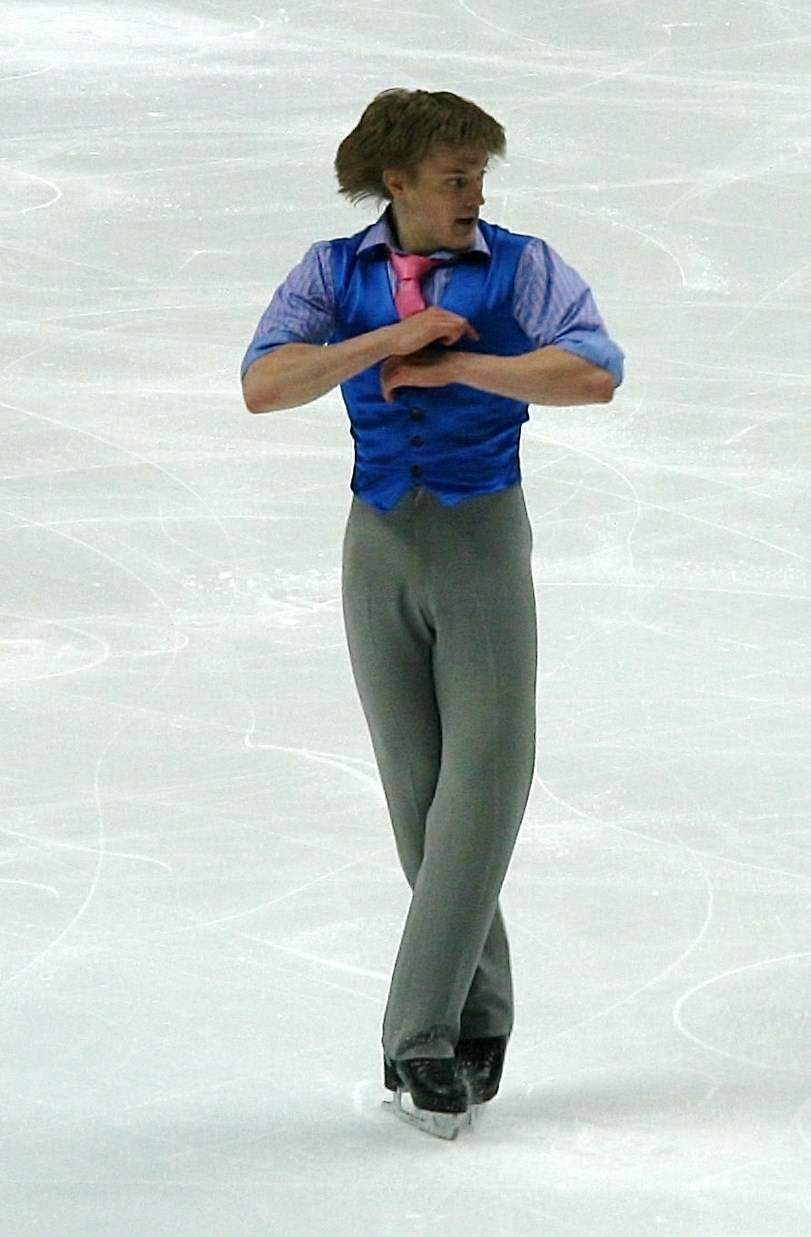
\includegraphics[width=0.3\textwidth]{chapters/chp4_pics/skater.jpg}
\caption{\textit{A skater performs a spin and holds his arms in to increase rotational motion by reducing moment of inertia.}}
\label{fig:skater}
\end{figure}

\noindent Consider a flywheel in an engine. When designed with a larger moment of inertia, it more effectively smooths out the engine's power delivery by storing and releasing rotational energy. This application shows why the $r^2$ term appears in polar form: mass at twice the radius contributes four times as much to the moment of inertia. Engineers use these calculations to design flywheels that achieve the desired balance between energy storage capacity and overall weight. \\

\noindent Moments of inertia appear in several key equations in physics:
\begin{itemize}
   \item Rotational Kinetic Energy: $E = \frac{1}{2}I\omega^2$, where $\omega$ is angular velocity
   \item Torque: $\tau = I\alpha$, where $\alpha$ is angular acceleration \index{Torque}
   \item Angular Momentum: $L = I\omega$ \index{Angular Momentum}
   \item Period of Rotation: $T = 2\pi\sqrt{\frac{I}{k}}$ for a torsional oscillator with spring constant $k$
\end{itemize}

\exampleline
\begin{example}
Elijah the Prophet, a legendary DJ, is designing a custom turntable platter—the rotating disc that holds vinyl records. The platter is shaped like an annular region (a washer shape) with inner radius $r = 1$ inch and outer radius $r = 6$ inches. To ensure smooth playback, the platter's density increases quadratically with radius according to $\rho(r) = kr^2$ ounces/inch$^2$, where $k$ is a constant. If the total mass of the platter is 20 ounces:

\begin{enumerate}
   \item Find the value of $k$.
   \item Calculate the moment of inertia $I_z$ about the turntable's axis of rotation.
   \item If the turntable spins at $33\frac{1}{3}$ RPM (rotations per minute), find its rotational kinetic energy in inch-ounces.
\end{enumerate}

\begin{solution}
\begin{enumerate}
   \item First, let's find $k$ using the total mass equation in polar coordinates:
   \[
   M = \int_0^{2\pi} \int_1^6 \rho(r)r\,dr\,d\theta = \int_0^{2\pi} \int_1^6 kr^3\,dr\,d\theta = 20
   \]
   
   Evaluating the integrals:
   \[
   2\pi k \left[\frac{r^4}{4}\right]_1^6 = 20
   \]
   \[
   2\pi k \left(\frac{1296}{4} - \frac{1}{4}\right) = 20
   \]
   \[
   2\pi k(324 - \frac{1}{4}) = 20
   \]
   
   Therefore:
   \[
   k = \frac{20}{2\pi(323.75)} \approx 0.0098 \text{ oz/inch}^4
   \]

   \item The moment of inertia about the $z$-axis is:
   \[
   I_z = \int_0^{2\pi} \int_1^6 r^2\rho(r)r\,dr\,d\theta = \int_0^{2\pi} \int_1^6 kr^5\,dr\,d\theta
   \]
   
   Substituting our value of $k$:
   \[
   I_z = 2\pi k \left[\frac{r^6}{6}\right]_1^6 = 2\pi \cdot \frac{20}{2\pi(323.75)} \cdot \left(\frac{46656}{6} - \frac{1}{6}\right)
   \]
   \[
   I_z = \frac{20}{323.75} \cdot 7776 \approx 480 \text{ oz}\cdot\text{inch}^2
   \]

   \item The angular velocity at $33\frac{1}{3}$ RPM is:
   \[
   \omega = \frac{100}{3} \cdot \frac{2\pi}{60} = \frac{10\pi}{9} \text{ rad/s}
   \]
   
   The rotational kinetic energy is:
   \[
   E = \frac{1}{2}I_z\omega^2 = \frac{1}{2}(480)\left(\frac{10\pi}{9}\right)^2 \approx 2926 \text{ oz}\cdot\text{inch}^2/\text{s}^2
   \]
\end{enumerate}

\noindent This high moment of inertia helps maintain consistent playback speed, as the platter's substantial rotational inertia resists changes in angular velocity. The quadratic density increase toward the outer edge—similar to putting weights around a turntable's perimeter—maximizes this stabilizing effect.
\end{solution}
\end{example}
\exampleline
\begin{example}
A robotic arm at a manufacturing plant rotates components on a flat mounting plate. The rectangular plate measures 40 cm × 30 cm and has a base density of $\rho_0 = 2$ g/cm$^2$. To optimize the rotation dynamics, the plate's density varies according to $\rho(x,y) = \rho_0(1 + \frac{x^2}{100})$ g/cm$^2$, where $x$ is measured in centimeters from the plate's vertical centerline. The system rotates with an initial angular velocity of $\omega_0 = 2\pi$ rad/s but must decelerate to a stop within time $t$ using a constant torque $\tau$.

\begin{enumerate}
   \item Calculate the moment of inertia $I_z$ about the central vertical axis.
   \item Using the rotational form of Newton's Second Law, $\tau = I\alpha$, find the required torque to bring the plate to rest in 3 seconds.
   \item What is the total angular displacement during this deceleration? Use the equation $\theta = \omega_0t + \frac{1}{2}\alpha t^2$.
\end{enumerate}

\begin{solution}
\begin{enumerate}
   \item Setting up coordinates with the origin at the center of the plate, our region is $R = [-20,20] \times [-15,15]$ in centimeters. For $I_z$:
   \[
   I_z = \iint_R (x^2 + y^2)\rho_0\left(1 + \frac{x^2}{100}\right)\,dA
   \]
   \[
   = \rho_0\int_{-20}^{20}\int_{-15}^{15}(x^2 + y^2)\left(1 + \frac{x^2}{100}\right)\,dy\,dx
   \]
   
   Breaking this into parts and evaluating:
   \[
   I_z = 2(754,000) = 1,508,000 \text{ g}\cdot\text{cm}^2
   \]
   
   Converting to SI units:
   \[
   I_z = 1,508,000 \times 10^{-7} = 0.1508 \text{ kg}\cdot\text{m}^2
   \]

   \item For constant deceleration from $\omega_0$ to 0 in time $t$:
   \[
   \alpha = \frac{\omega_\text{final} - \omega_0}{t} = \frac{0 - 2\pi}{3} = -\frac{2\pi}{3} \text{ rad/s}^2
   \]
   
   Using $\tau = I\alpha$:
   \[
   \tau = 0.1508 \cdot \left(-\frac{2\pi}{3}\right) = -0.316 \text{ N}\cdot\text{m}
   \]

   \item For the total angular displacement:
   \[
   \theta = \omega_0t + \frac{1}{2}\alpha t^2 = 2\pi(3) + \frac{1}{2}\left(-\frac{2\pi}{3}\right)(3)^2
   \]
   \[
   = 6\pi - 3\pi = 3\pi \text{ rad} = 540^\circ
   \]
\end{enumerate}
\end{solution}
\end{example}
\exampleline


\subsection*{Average Values over Two-Dimensional Regions} \index{Average Value} \index{Average Distribution}

\noindent We took a sneak peek of this concept when we looked at average efficiency in the previous lecture -- When analyzing quantities that vary over a region, we often need to find their average values. Just as the average of discrete values is found by summing and dividing by the count, the average value of a continuous function $f(x,y)$ over a region $R$ is found by integrating and dividing by the region's area:
\[
f_{avg} = \frac{\iint_R f(x,y)\,dA}{\iint_R dA}
\]

\noindent This formula has a natural physical interpretation: the denominator $\iint_R dA$ represents the total area of region $R$, while the numerator accumulates the value of $f$ over that same region. For example, if $f(x,y)$ represents temperature at each point on a metal plate, this formula gives the plate's average temperature. \\

\noindent For non-uniform materials where density varies across the region, we often use a weighted average:
\[
f_{avg} = \frac{\iint_R f(x,y)\rho(x,y)\,dA}{\iint_R \rho(x,y)\,dA}
\]

\noindent Here, $\rho(x,y)$ acts as a weighting function, giving more importance to regions of higher density. This weighted form finds frequent use in engineering applications, from calculating the center of mass of a plate with varying density to determining average stress in composite materials. \\

\noindent Both formulas extend naturally to polar coordinates through the appropriate change of variables, with $dA = r\,dr\,d\theta$. This proves particularly useful when working with circular or radially symmetric regions where the function or density varies with distance from a central point.

\subsection*{Surface Area and Physical Interfaces} \index{Surface Area}

\noindent The motivation for surface area begins with the arc length formula that we learned in Chapter 2. Recall that for a curve $y = f(x)$, we found its arc length by considering how differential changes in $x$ and $y$ contribute to the length of an infinitesimal segment:
\[
ds = \sqrt{dx^2 + dy^2} = \sqrt{1 + \left(\frac{dy}{dx}\right)^2}\,dx
\]
This gave us the arc length formula $L = \int_a^b \sqrt{1 + \left(\frac{dy}{dx}\right)^2}\,dx$. \\

\noindent For a surface $z = f(x,y)$, we follow similar reasoning. Consider a small patch of surface above a region $dA$ in the $xy$-plane. As we move in both $x$ and $y$ directions, the surface rises according to its partial derivatives. The actual area of this patch must account for these slopes in both directions, leading to:
\[
dA_{\text{surface}} = \sqrt{1 + \left(\frac{\partial f}{\partial x}\right)^2 + \left(\frac{\partial f}{\partial y}\right)^2}\,dA
\]

\noindent Integrating over the region $R$ gives us the total surface area:
\[
A = \iint_R \sqrt{1 + \left(\frac{\partial f}{\partial x}\right)^2 + \left(\frac{\partial f}{\partial y}\right)^2}\,dA
\]


\begin{figure}[H]
\centering
\tdplotsetmaincoords{60}{120}

\begin{tikzpicture}[tdplot_main_coords, scale=1.7,
declare function={
    surfacefn(\x,\y)=1+0.2*sin(deg(2*\x))*cos(deg(2*\y));
}]

% Axes
\draw[->] (0,0,0) -- (3,0,0) node[right] {$x$};
\draw[->] (0,0,0) -- (0,3,0) node[right] {$y$};
\draw[->] (0,0,0) -- (0,0,2) node[above] {$z$};

% Surface grid
\foreach \x in {0,0.5,...,3} {
    \draw[blue!20] plot[variable=\y,domain=0:3,samples=30] 
    (\x,\y,{surfacefn(\x,\y)});
}
\foreach \y in {0,0.5,...,3} {
    \draw[blue!20] plot[variable=\x,domain=0:3,samples=30] 
    (\x,\y,{surfacefn(\x,\y)});
}

% Surface element parameters
\def\px{1.0}
\def\py{1.0}
\def\dxsize{0.4}
\def\dysize{0.4}

% Surface element corners
\coordinate (P1) at (\px,\py,{surfacefn(\px,\py)});
\coordinate (P2) at ({\px+\dxsize},\py,{surfacefn(\px+\dxsize,\py)});
\coordinate (P3) at ({\px+\dxsize},{\py+\dysize},{surfacefn(\px+\dxsize,\py+\dysize)});
\coordinate (P4) at (\px,{\py+\dysize},{surfacefn(\px,\py+\dysize)});

% Fill surface element
\fill[blue!40,opacity=0.6] (P1) -- (P2) -- (P3) -- (P4) -- cycle;

% Draw element edges
\draw[blue,thick] (P1) -- (P2) -- (P3) -- (P4) -- cycle;

% Tangent vectors u and v
\draw[->,ultra thick,orange] (P1) -- (P2) node[midway, above, sloped] {};
\draw[->,ultra thick,green] (P1) -- (P4) node[midway, left] {};

% Normal vector (cross product)
\draw[->,ultra thick,red] ($(P1)!0.5!(P3)$) --
    ($(P1)!0.5!(P3) + (0,0,0.5)$) node[midway, right] {};

\node at (0,2,2) {$z=f(x,y)$};

% Legend outside the plot area to the right
\node[draw, anchor=west, fill=white, opacity=0.9, right=of current bounding box.east, xshift=0.5cm] {
    \begin{tabular}{ll}
        \textcolor{orange}{$\longrightarrow$} & $\vec{u}$ \\
        \textcolor{green}{$\longrightarrow$} & $\vec{v}$ \\
        \textcolor{red}{$\longrightarrow$} & $\vec{u} \times \vec{v}$ \\
        \textcolor{blue}{\rule{1cm}{2pt}} & $dS$ \\
    \end{tabular}
};

\end{tikzpicture}
\caption{\textit{The surface area element $dS$ arises from the cross product of tangent vectors 
$\vec{u} = (dx, 0, \frac{\partial f}{\partial x}dx)$ and $\vec{v} = (0, dy, \frac{\partial f}{\partial y}dy)$. 
Their cross product gives $dS = \|\vec{u} \times \vec{v}\| = \sqrt{1 + \left(\frac{\partial f}{\partial x}\right)^2 + \left(\frac{\partial f}{\partial y}\right)^2}\,dx\,dy$.}}
\end{figure}


\noindent If our surface is better described using polar coordinates, we can transform this formula. For $z = f(r,\theta)$, the surface area becomes:
\[
A = \iint_R \sqrt{1 + \left(\frac{\partial f}{\partial r}\right)^2 + \frac{1}{r^2}\left(\frac{\partial f}{\partial \theta}\right)^2}\,r\,dr\,d\theta
\]

\noindent Thus, this shows us that surface area is just arc-length in three dimensions. This pattern also generalizes. For a \textit{hypersurface} in $n$ dimensions given by a function of $n-1$ variables, the hypersurface area becomes:
\[
A = \int_R \sqrt{1 + \sum_{i=1}^{n-1} \left(\frac{\partial f}{\partial x_i}\right)^2}\,dA
\]

\noindent This generalization finds applications in physics and engineering. The bad thing about these formulae is that the integral is usually too hard to solve, so we will frequently have to rely on numerical methods and/or the all seeing eye: Wolfram Alpha. \\

\noindent Let us now explore these formulae with a concrete example:

\exampleline
\begin{example}
In architecture, hyperbolic paraboloids (saddle surfaces) are used to create striking modern designs that combine aesthetics with structural efficiency. Consider a surface given by $z = \frac{x^2}{4} - \frac{y^2}{9}$ over the region $R = [-1,1] \times [-2,2]$.

\begin{enumerate}
   \item Set up (but do not evaluate) the surface area integral.
   \item Use the fact that this integral evaluates to approximately 8.56 square units to discuss the efficiency of this architectural form.
\end{enumerate}

\begin{solution}
Let's solve this step by step:

\begin{enumerate}
   \item First, we compute the partial derivatives:
   \[
   \frac{\partial z}{\partial x} = \frac{x}{2}, \quad \frac{\partial z}{\partial y} = -\frac{2y}{9}
   \]

   The surface area is given by:
   \[
   A = \iint_R \sqrt{1 + \left(\frac{\partial z}{\partial x}\right)^2 + \left(\frac{\partial z}{\partial y}\right)^2}\,dA
   \]

   Substituting the partial derivatives:
   \[
   A = \iint_R \sqrt{1 + \frac{x^2}{4} + \frac{4y^2}{81}}\,dA
   \]

   Since the integrand $\sqrt{1 + \frac{x^2}{4} + \frac{4y^2}{81}}$ is even in both $x$ and $y$, we can integrate over the first quadrant and multiply by 4:
   \[
   A = 4\int_0^1\int_0^2 \sqrt{1 + \frac{x^2}{4} + \frac{4y^2}{81}}\,dy\,dx
   \]

   \item The numerical evaluation of this integral yields $A \approx 8.56$ square units. This relatively small surface area compared to the region covered ($8$ square units in the $xy$-plane) demonstrates why hyperbolic paraboloids are efficient architectural forms. The surface area is only about 7\% more than the flat projection, making them materially economical while their curvature provides structural advantages through geometric stiffness.
\end{enumerate}
\end{solution}
\end{example}
\exampleline


\newpage


\lecture{Triple Integrals}

\noindent Imagine you need to find the total mass of an irregularly shaped rock whose density varies throughout, or the total charge inside a thundercloud. These are naturally three-dimensional problems that require integrating a function over a solid region -- and that is exactly what triple integrals do.\\ \\

\noindent Having explored integration over regions in the plane, we now extend our understanding to higher dimensions. Recall that double integrals allowed us to find areas under surfaces by integrating a function $f(x,y)$ over a region $R$, producing outputs in units of ``function $\times$ area''. For instance, when integrating a constant height function $f(x,y) = h$ over a region $R$, we obtained volume: $V = h\iint_R dA$. \\

\noindent Triple integrals follow this pattern but work in three dimensions. When we integrate a function $f(x,y,z)$ over a solid region $E$ in space, our output will have units of ``function $\times$ volume''. At first glance, this might suggest we are limited to producing quantities measured in spatial units to the fourth power—a type of hypervolume. However, just as we saw with density functions producing mass ($\text{g/cm}^3 \times \text{cm}^3 = \text{g}$), the integrand can carry rates that combine with volume in various ways. \\

\noindent Consider, for example, the second moment of inertia tensor in engineering, which has units of $\text{kg}\cdot\text{m}^2$. When analyzing rotating bodies, we might integrate $\rho(x,y,z)(y^2 + z^2)$ to find the moment of inertia about the $x$-axis. Here, the density ($\text{kg}/\text{m}^3$) combines with squared distance terms ($\text{m}^2$) and volume ($\text{m}^3$) to produce the correct units. Or in dynamics, when studying jerk (the rate of change of acceleration), we might integrate a function with units $\text{m}/\text{s}^3$ over a volume to find total change in momentum rate. The power of triple integrals lies in this flexibility to handle various physical quantities through appropriate choice of integrand, practical implications of which will be explored in more detail in the coming lectures in this chapter. The good news for us in this introduction is that we will use almost identical machinery to what we used with double integrals -- there are not many more layers of complexity to add when generalizing double integrals to triple and beyond.


\subsection*{Definition and Computation}

\noindent Consider a solid region $E$ in three-dimensional space and a function $f(x,y,z)$ defined over this region. Just as we built double integrals from the concept of summing over rectangles, we construct triple integrals by summing over small rectangular boxes called volume elements. Each volume element has dimensions $\Delta x$, $\Delta y$, and $\Delta z$, giving it a volume of $\Delta V = \Delta x\Delta y\Delta z$. \\

\noindent When constructing our Riemann sum, we must choose a sample point $(x_i^*, y_i^*, z_i^*)$ within each box. Where single integrals required choosing a point on a line segment and double integrals required choosing a point in a rectangle, triple integrals require selecting a point within a rectangular box. This point could be at any corner of the box (there are eight corners), at the center of the box, or at any other location within the box. For each such box with its chosen sample point, we compute $f(x_i^*, y_i^*, z_i^*)\Delta V_i$. \\

\noindent As all dimensions of these boxes approach zero (that is, as $\Delta x$, $\Delta y$, and $\Delta z$ all approach zero), their sum approaches the triple integral:
\[
\iiint_E f(x,y,z)\,dV = \lim_{n \to \infty} \sum_{i=1}^n f(x_i^*, y_i^*, z_i^*)\Delta V_i
\]

\noindent Just as with double integrals, different choices of sample points might give different approximations, but all reasonable choices converge to the same limit as the box dimensions approach zero. The differential volume element $dV = dx\,dy\,dz$ represents the limiting case of $\Delta V$ as all dimensions approach zero. The units of $dV$ will always be cubic units (cubic meters, cubic centimeters, etc.), while the units of $f(x,y,z)$ could vary depending on the application. \\

\noindent For a rectangular box $E = [a,b] \times [c,d] \times [p,q]$, we can write an iterated integral:
\[
\iiint_E f(x,y,z)\,dV = \int_a^b\int_c^d\int_p^q f(x,y,z)\,dz\,dy\,dx
\]

\noindent This can be evaluated in any order—Fubini's Theorem extends naturally to three dimensions:
\[
\int_a^b\int_c^d\int_p^q f(x,y,z)\,dz\,dy\,dx = \int_p^q\int_c^d\int_a^b f(x,y,z)\,dx\,dy\,dz
\]
and similarly for any other permutation of the variables. The choice of order, while not affecting the result, often significantly impacts the complexity of computation. \\

\noindent For example, if we're computing the mass of a solid where density varies with height, integrating with respect to $z$ first might simplify our work. If instead the density varies with distance from an axis, we might prefer cylindrical coordinates—a system we'll explore shortly.


\subsection*{Types of Integration Regions} \index{Triple Integral Regions}   

\noindent When integrating over general three-dimensional regions, we must carefully analyze the geometry to determine appropriate bounds of integration. Just as with double integrals, we can often view a region from different perspectives, leading to distinct but equivalent ways to set up our integral. Let's examine the three fundamental types of regions we encounter. \\

\noindent \textbf{Type I Regions:} \index{Triple Integral Regions!Type I Regions} These regions are defined by viewing the solid from the side, looking perpendicular to the $xy$-plane. The region is bounded above and below by surfaces $z = g_2(x,y)$ and $z = g_1(x,y)$ respectively, where these surfaces sit above a region $R$ in the $xy$-plane. For such regions:
\[
\iiint_E f(x,y,z)\,dV = \iint_R\int_{g_1(x,y)}^{g_2(x,y)} f(x,y,z)\,dz\,dA
\]

\begin{figure}[H]
\centering
\tdplotsetmaincoords{60}{120} % Adjust viewing angle for Type I
\begin{tikzpicture}[tdplot_main_coords, scale=3]
    % Define coordinates
    \coordinate (O) at (0,0,0);
    \coordinate (A) at (1,0,0);
    \coordinate (B) at (1,1,0);
    \coordinate (C) at (0,1,0);
    
    % Base rectangle R in xy-plane
    \draw[thick, fill=gray!20, opacity=0.5] (0,0,0) -- (1,0,0) -- (1,1,0) -- (0,1,0) -- cycle;
    
    % Bottom surface z = g1(x,y)
    \draw[thick, fill=blue!20, opacity=0.5] (0,0,0) -- (1,0,0) -- (1,1,0) -- (0,1,0) -- cycle;
    
    % Top surface z = g2(x,y)
    \draw[thick, fill=red!20, opacity=0.5] (0,0,1) -- (1,0,1) -- (1,1,1) -- (0,1,1) -- cycle;
    
    % Connect base to top with dashed lines
    \draw[thick, dashed] (0,0,0) -- (0,0,1);
    \draw[thick, dashed] (1,0,0) -- (1,0,1);
    \draw[thick, dashed] (1,1,0) -- (1,1,1);
    \draw[thick, dashed] (0,1,0) -- (0,1,1);
    
    % Axes
    \draw[thick,->] (0,0,0) -- (1.5,0,0) node[anchor=north east]{$x$};
    \draw[thick,->] (0,0,0) -- (0,1.5,0) node[anchor=north west]{$y$};
    \draw[thick,->] (0,0,0) -- (0,0,1.5) node[anchor=south]{$z$};
    
    % Labels
    \node at (0.3,0.3,0) {$R$};
    \node at (0.5,0.5,1.1) {$z = g_2(x,y)$};
    \node at (0.5,0.5,-0.1) {$z = g_1(x,y)$};
\end{tikzpicture}
\caption{\textit{A Type I region bounded by two surfaces above a region $R$ in the $xy$-plane.}}
\end{figure}
 \index{Triple Integral Regions!Type II Regions} 
\noindent \textbf{Type II Regions:} These regions are viewed by looking perpendicular to the $yz$-plane, bounded by surfaces $x = h_1(y,z)$ and $x = h_2(y,z)$ over a region $R$ in the $yz$-plane. Here:
\[
\iiint_E f(x,y,z)\,dV = \iint_R\int_{h_1(y,z)}^{h_2(y,z)} f(x,y,z)\,dx\,dA
\]

\begin{figure}[H]
\centering
\tdplotsetmaincoords{60}{60} % Existing correct view for Type II
\begin{tikzpicture}[tdplot_main_coords, scale=3]

    % Define coordinates
    \coordinate (O) at (0,0,0);
    \coordinate (A) at (1,0,0);
    \coordinate (B) at (1,1,0);
    \coordinate (C) at (0,1,0);
    
    % Base rectangle R in yz-plane
    \draw[thick, fill=gray!20, opacity=0.5] (0,0,0) -- (0,1,0) -- (0,1,1) -- (0,0,1) -- cycle;
    
    % Bottom surface x = h1(y,z) (x = 0)
    \draw[thick, fill=blue!20, opacity=0.5] (0,0,0) -- (0,1,0) -- (0,1,1) -- (0,0,1) -- cycle;
    
    % Top surface x = h2(y,z) (x = 1)
    \draw[thick, fill=red!20, opacity=0.5] (1,0,0) -- (1,1,0) -- (1,1,1) -- (1,0,1) -- cycle;
    
    % Connect base to top with dashed lines
    \draw[thick, dashed] (0,0,0) -- (1,0,0);
    \draw[thick, dashed] (0,1,0) -- (1,1,0);
    \draw[thick, dashed] (0,1,1) -- (1,1,1);
    \draw[thick, dashed] (0,0,1) -- (1,0,1);
    
    % Axes
    \draw[thick,->] (0,0,0) -- (1.5,0,0) node[anchor=north east]{$x$};
    \draw[thick,->] (0,0,0) -- (0,1.5,0) node[anchor=north west]{$y$};
    \draw[thick,->] (0,0,0) -- (0,0,1.5) node[anchor=south]{$z$};
    
    % Labels
    \node at (0,0.3,0.3) {$R$};
    \node at (1.5,0.1,0.5) {$x = h_2(y,z)$};
    \node at (-0.2,0.6,0.5) {$x = h_1(y,z)$};

\end{tikzpicture}
\caption{\textit{A Type II region bounded by surfaces viewed from the $yz$-plane.}}
\end{figure}
 \index{Triple Integral Regions!Type III Regions} 
\noindent \textbf{Type III Regions:} These regions are viewed by looking perpendicular to the $xz$-plane, bounded by surfaces $y = k_1(x,z)$ and $y = k_2(x,z)$ over a region $R$ in the $xz$-plane:
\[
\iiint_E f(x,y,z)\,dV = \iint_R\int_{k_1(x,z)}^{k_2(x,z)} f(x,y,z)\,dy\,dA
\]

\begin{figure}[H]
\centering
\tdplotsetmaincoords{60}{30} % Adjust viewing angle for Type III
\begin{tikzpicture}[tdplot_main_coords, scale=3]
    % Define coordinates
    \coordinate (O) at (0,0,0);
    \coordinate (A) at (1,0,0);
    \coordinate (B) at (1,0,1);
    \coordinate (C) at (0,0,1);
    
    % Base rectangle R in xz-plane
    \draw[thick, fill=gray!20, opacity=0.5] (0,0,0) -- (1,0,0) -- (1,0,1) -- (0,0,1) -- cycle;
    
    % Bottom surface y = k1(x,z)
    \draw[thick, fill=blue!20, opacity=0.5] (0,0,0) -- (1,0,0) -- (1,0,1) -- (0,0,1) -- cycle;
    
    % Top surface y = k2(x,z)
    \draw[thick, fill=red!20, opacity=0.5] (0,1,0) -- (1,1,0) -- (1,1,1) -- (0,1,1) -- cycle;
    
    % Connect base to top with dashed lines
    \draw[thick, dashed] (0,0,0) -- (0,1,0);
    \draw[thick, dashed] (1,0,0) -- (1,1,0);
    \draw[thick, dashed] (1,0,1) -- (1,1,1);
    \draw[thick, dashed] (0,0,1) -- (0,1,1);
    
    % Axes
    \draw[thick,->] (0,0,0) -- (1.5,0,0) node[anchor=north east]{$x$};
    \draw[thick,->] (0,0,0) -- (0,3,0) node[anchor=north west]{$y$};
    \draw[thick,->] (0,0,0) -- (0,0,1.5) node[anchor=south]{$z$};
    
    % Labels
    \node at (0.5,0,0.45) {$R$};
    \node at (1.5,1.1,0.5) {$y = k_2(x,z)$};
    \node at (0.65,-0.1,0.3) {$y = k_1(x,z)$};
\end{tikzpicture}
\caption{\textit{A Type III region bounded by surfaces viewed from the $xz$-plane.}}
\end{figure}


\exampleline
\begin{example}
\begin{enumerate}
   \item Find $\displaystyle\iiint_E (x^2 + y^2)\,dV$ where $E$ is the rectangular box $[0,1] \times [1,2] \times [-1,3]$.
   \item Find $\displaystyle\iiint_E xyz\,dV$ where $E$ is the region bounded below by the $xy$-plane ($z = 0$) and above by the plane $z = 2 - x - y$ in the first octant.
\end{enumerate}

\begin{solution}
\begin{enumerate}
   \item For the rectangular box:

   \begin{figure}[H]
   \centering
   \tdplotsetmaincoords{60}{110}
   \begin{tikzpicture}[tdplot_main_coords,scale=.9]
       % Axes for rectangular box
       \draw[->] (0,0,0) -- (2,0,0) node[right] {$x$};
       \draw[->] (0,0,0) -- (0,3,0) node[right] {$y$};
       \draw[->] (0,0,0) -- (0,0,4) node[left] {$z$};
       
       % Draw back faces (drawn first)
       \fill[blue!20,opacity=0.3] (0,2,-1) -- (0,2,3) -- (1,2,3) -- (1,2,-1) -- cycle;
       \fill[blue!20,opacity=0.3] (1,1,-1) -- (1,2,-1) -- (1,2,3) -- (1,1,3) -- cycle;
       
       % Draw bottom
       \fill[blue!30,opacity=0.3] (0,1,-1) -- (1,1,-1) -- (1,2,-1) -- (0,2,-1) -- cycle;
       
       % Draw front faces
       \fill[blue!40,opacity=0.3] (0,1,-1) -- (0,1,3) -- (0,2,3) -- (0,2,-1) -- cycle;
       \fill[blue!40,opacity=0.3] (0,1,-1) -- (1,1,-1) -- (1,1,3) -- (0,1,3) -- cycle;
       
       % Draw top
       \fill[blue!50,opacity=0.3] (0,1,3) -- (1,1,3) -- (1,2,3) -- (0,2,3) -- cycle;
       
       % Draw edges
       \draw[blue,thick] (0,1,-1) -- (1,1,-1) -- (1,2,-1) -- (0,2,-1) -- cycle;
       \draw[blue,thick] (0,1,3) -- (1,1,3) -- (1,2,3) -- (0,2,3) -- cycle;
       \draw[blue,thick] (0,1,-1) -- (0,1,3);
       \draw[blue,thick] (1,1,-1) -- (1,1,3);
       \draw[blue,thick] (1,2,-1) -- (1,2,3);
       \draw[blue,thick] (0,2,-1) -- (0,2,3);
       
       % Labels for bounds
       \node[below] at (0.5,1.5,-1.4) {$[0,1] \times [1,2] \times [-1,3]$};
   \end{tikzpicture}
   \caption{\textit{Problem 1: Rectangular box region}}
   \end{figure}

   \begin{align*}
   \iiint_E (x^2 + y^2)\,dV &= \int_0^1\int_1^2\int_{-1}^3 (x^2 + y^2)\,dz\,dy\,dx \\[1ex]
   &= \int_0^1\int_1^2 (x^2 + y^2)[z]_{-1}^3\,dy\,dx \\[1ex]
   &= 4\int_0^1\int_1^2 (x^2 + y^2)\,dy\,dx \\[1ex]
   &= 4\int_0^1 \left[x^2y + \frac{y^3}{3}\right]_1^2\,dx \\[1ex]
   &= 4\int_0^1 \left(x^2(2-1) + \frac{8}{3} - \frac{1}{3}\right)\,dx \\[1ex]
   &= 4\left[\frac{x^3}{3} + \frac{7x}{3}\right]_0^1 = \frac{32}{3}
   \end{align*}

   \item For the region in the first octant:

   \begin{figure}[H]
   \centering
   \tdplotsetmaincoords{60}{110}
   \begin{tikzpicture}[tdplot_main_coords,scale=1.2]
       % Axes for slanted plane region
       \draw[->] (0,0,0) -- (3,0,0) node[right] {$x$};
       \draw[->] (0,0,0) -- (0,3,0) node[right] {$y$};
       \draw[->] (0,0,0) -- (0,0,3) node[left] {$z$};
       
       % Fill base triangle
       \fill[blue!20,opacity=0.3] (0,0,0) -- (2,0,0) -- (0,2,0) -- cycle;
       
       % Fill side faces
       \fill[blue!30,opacity=0.3] (0,0,0) -- (2,0,0) -- (2,0,0) -- (0,0,2) -- cycle;
       \fill[blue!30,opacity=0.3] (0,0,0) -- (0,2,0) -- (0,0,2) -- cycle;
       \fill[blue!40,opacity=0.3] (0,0,2) -- (2,0,0) -- (0,2,0) -- cycle;
       
       % Draw edges
       \draw[blue,thick] (0,0,0) -- (2,0,0) -- (0,2,0) -- cycle;
       \draw[blue,thick] (0,0,0) -- (0,0,2);
       \draw[blue,thick,dashed] (0,0,2) -- (2,0,0);
       \draw[blue,thick,dashed] (0,0,2) -- (0,2,0);
       
       % Label the plane
       \node at (1,3,1.5) {$z = 2-x-y$};
       \node at (0.5,0.5,0) {$z = 0$};
   \end{tikzpicture}
   \caption{\textit{Problem 2: Region bounded by plane $z = 2-x-y$ and $xy$-plane}}
   \end{figure}

\noindent The bounds are in the first octant bounded below by the $xy$-plane ($z=0$) and above by the plane $z=2-x-y$. From the $xy$-plane projection, we see $x$ ranges from $0$ to $2$, and for each fixed $x$, $y$ ranges from $0$ to $2-x$. For each fixed $x$ and $y$, $z$ then ranges from $0$ to $2-x-y$, giving the triple integral's bounds.

   \begin{align*}
   \iiint_E xyz\,dV &= \int_0^2\int_0^{2-x}\int_0^{2-x-y} xyz\,dz\,dy\,dx \\[1ex]
   &= \int_0^2\int_0^{2-x} xy\left[\frac{z^2}{2}\right]_0^{2-x-y}\,dy\,dx \\[1ex]
   &= \frac{1}{2}\int_0^2\int_0^{2-x} xy(2-x-y)^2\,dy\,dx
   \end{align*}
   
   Let $u = 2-x-y$, so $y = 2-x-u$ and $dy = -du$. When $y = 0$, $u = 2-x$; when $y = 2-x$, $u = 0$. This gives:
   \begin{align*}
   &= \frac{1}{2}\int_0^2 x\int_{2-x}^0 (2-x-u)u^2(-du)\,dx \\[1ex]
   &= \frac{1}{2}\int_0^2 x\left[(2-x)\frac{u^3}{3} - \frac{u^4}{4}\right]_0^{2-x}\,dx \\[1ex]
   &= \frac{1}{24}\int_0^2 x(2-x)^4\,dx = \frac{4}{45}
   \end{align*}
\end{enumerate}
\end{solution}
\end{example}
\exampleline

\begin{example}
Find $\displaystyle\iiint_E 1\,dV$ where $E$ is the region bounded by the intersection of two perpendicular unit cylinders $x^2 + y^2 = 1$ and $x^2 + z^2 = 1$.

\begin{solution}

%https://commons.wikimedia.org/wiki/File:Steinmetz-cc.svg
%https://commons.wikimedia.org/wiki/File:Steinmetz-cc2-ag.svg
\begin{figure}[H]
\centering
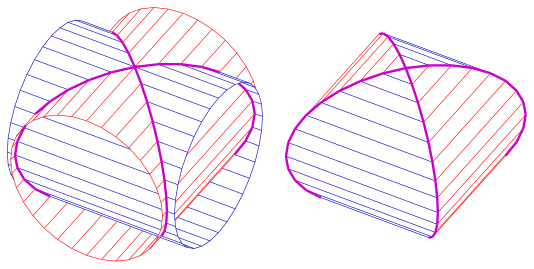
\includegraphics[width=0.6\textwidth]{chapters/chp4_pics/steinmetz.png}
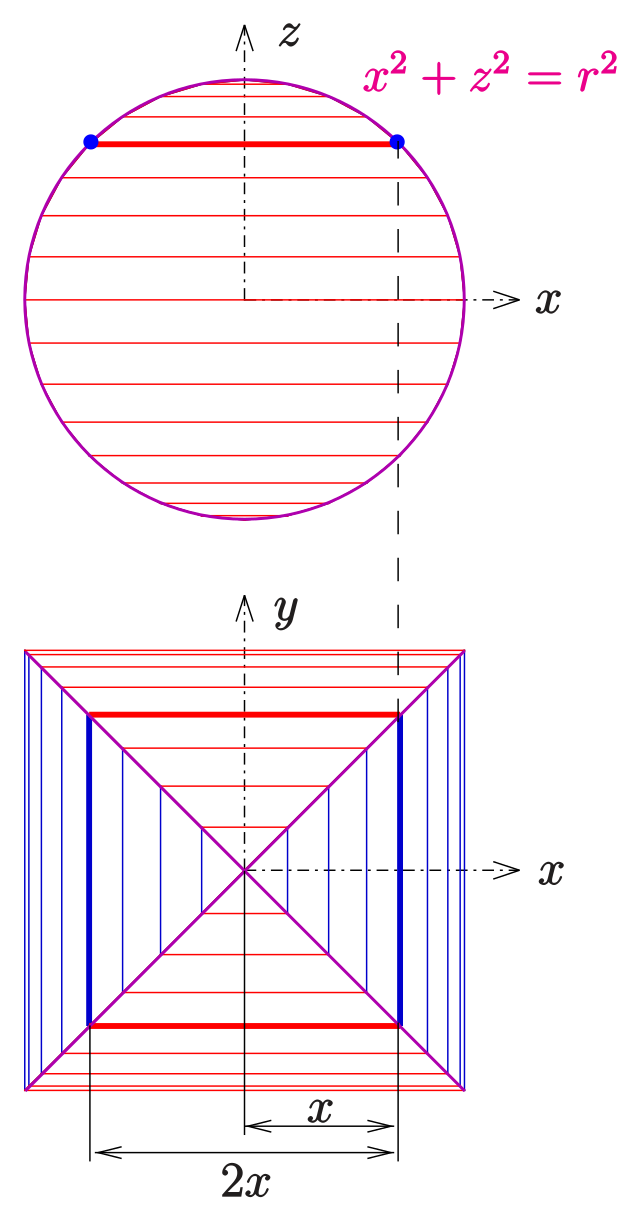
\includegraphics[width=0.25\textwidth]{chapters/chp4_pics/steinmetz-side.png}
\caption{\textit{The Steinmetz solid, formed by the intersection of two perpendicular unit cylinders $x^2 + y^2 = 1$ and $x^2 + z^2 = 1$.}}
\label{fig:steinmetz}
\end{figure}

\noindent Due to the symmetry of the region across all coordinate planes, we can evaluate the integral in the first octant and multiply by 8. In the first octant, $x$ ranges from $0$ to $1$, and for each fixed $x$, both $y$ and $z$ range from $0$ to $\sqrt{1-x^2}$ due to the circular cross-sections of the cylinders (found by solving our two equations for $y$ and $z$):
\begin{align*}
\iiint_E 1\,dV &= 8\int_0^1\int_0^{\sqrt{1-x^2}}\int_0^{\sqrt{1-x^2}} 1\,dz\,dy\,dx \\[1ex]
&= 8\int_0^1\int_0^{\sqrt{1-x^2}} \sqrt{1-x^2}\,dy\,dx \\[1ex]
&= 8\int_0^1 (1-x^2)\,dx \\[1ex]
&= 8\left[x - \frac{x^3}{3}\right]_0^1 = 8\left(1 - \frac{1}{3}\right) = \frac{16}{3}
\end{align*}
\end{solution}
\end{example}
\exampleline

\noindent The choice of which type to use for a given region often depends on the geometry of the bounding surfaces and the nature of the integrand. Many complex regions might require breaking the integral into parts and using different types for each part. Just as with double integrals, the goal is to choose the type that leads to the most straightforward computation. \\

\noindent However, for certain geometries—particularly those with circular or spherical symmetry—we'll find that alternative coordinate systems provide more natural representations. These systems, cylindrical and spherical coordinates, will be our next topic of study.

\subsection*{Coordinate Systems for Triple Integration}

\noindent The choice of coordinate system can dramatically simplify a triple integral computation. Just as we found polar coordinates useful for double integrals over circular regions, cylindrical and spherical coordinates provide natural frameworks for three-dimensional regions with certain types of symmetry. Let's examine these alternative coordinate systems and understand how they transform our integration process.

\subsubsection*{Cylindrical Coordinates}

\noindent As we learned in Chapter 1, cylindrical coordinates extend polar coordinates into three dimensions by adding a height coordinate. A point $(x,y,z)$ in rectangular coordinates is represented by coordinates $(r,\theta,z)$ in the cylindrical system:
\begin{align*}
x &= r\cos\theta \\
y &= r\sin\theta \\
z &= z
\end{align*}

\noindent The coordinate $r$ represents the distance from the point to the $z$-axis, $\theta$ measures the angle from the positive $x$-axis in the $xy$-plane, and $z$ gives the height above the $xy$-plane. This system naturally describes surfaces like cylinders, where $r$ is constant, and cones, where $z$ is proportional to $r$. \\

\noindent When converting a triple integral to cylindrical coordinates, we must account for how volume elements transform. A small rectangular box $dx\,dy\,dz$ becomes a curved wedge $r\,dr\,d\theta\,dz$. The factor of $r$ appears for the same reason it did in double integrals—as we move farther from the $z$-axis, the same angular increment $d\theta$ sweeps out a larger arc. Thus:
\[
\iiint_E f(x,y,z)\,dV = \iiint_E f(r\cos\theta, r\sin\theta, z)r\,dr\,d\theta\,dz
\]

\begin{figure}[H]
\centering
%Axis Angles
\tdplotsetmaincoords{70}{110}

%Macros
\pgfmathsetmacro{\rvec}{5}
\pgfmathsetmacro{\phivec}{45}
\pgfmathsetmacro{\zvec}{4}

\pgfmathsetmacro{\drvec}{1.5}
\pgfmathsetmacro{\dphivec}{20}
\pgfmathsetmacro{\dzvec}{1}

%Layers
\pgfdeclarelayer{background}
\pgfdeclarelayer{foreground}

\pgfsetlayers{background, main, foreground}

\begin{tikzpicture}[tdplot_main_coords]

%Coordinates
\coordinate (O) at (0,0,0);
%%
\cylindricalcoordinate{\rvec}{\phivec}{\zvec}{A}
\cylindricalcoordinate{\rvec}{\phivec}{(\zvec+\dzvec)}{B}
\cylindricalcoordinate{\rvec}{(\phivec+\dphivec)}{\zvec}{C}
\cylindricalcoordinate{\rvec}{(\phivec+\dphivec)}{(\zvec+\dzvec)}{D}
%%
\cylindricalcoordinate{(\rvec+\drvec)}{\phivec}{\zvec}{A'}
\cylindricalcoordinate{(\rvec+\drvec)}{\phivec}{(\zvec+\dzvec)}{B'}
\cylindricalcoordinate{(\rvec+\drvec)}{(\phivec+\dphivec)}{\zvec}{C'}
\cylindricalcoordinate{(\rvec+\drvec)}{(\phivec+\dphivec)}{(\zvec+\dzvec)}{D'}
%%%Nodes
%\node at (A) {A};
%\node at (B) {B};
%\node at (C) {C};
%\node at (D) {D};
%\node at (A') {A'};
%\node at (B') {B'};
%\node at (C') {C'};
%\node at (D') {D'};

%Axis
\begin{pgfonlayer}{background}
	\draw[thick,-latex] (0,0,0) -- (6,0,0) node[pos=1.1]{$x$};
	\draw[thick,-latex] (0,0,0) -- (0,6,0) node[pos=1.05]{$y$};
	\draw[thick,-latex] (0,0,0) -- (0,0,6) node[pos=1.05]{$z$};
\end{pgfonlayer}

%Vectors
\begin{pgfonlayer}{main}
	\draw[blue, thick] (O) -- (A);
	\draw[thick] (O) -- (Axy) node [pos=0.6, below left] {$r$};
	\draw (A) -- ($(A)-(Axy)$) node [left] {$z$};
	\draw (B) -- ($(A)-(Axy)+(0,0,\dzvec)$) node [left] {$z+dz$};
	\draw (D) -- ($(A)-(Axy)+(0,0,\dzvec)$);
\end{pgfonlayer}
\begin{pgfonlayer}{background}
	\draw[dashed] (C) -- ($(A)-(Axy)$) node [left] {$z$};
\end{pgfonlayer}

%Help Lines
\begin{pgfonlayer}{background}
	\draw (A) -- (Axy);
	\draw (A') -- (A'xy);
	\draw[thick] (Axy) -- (A'xy) node [pos=0.6, below left] {$dr$};
	%
	\draw (O) -- (D'xy);
	\draw[dashed] (C) -- (Dxy);	
	\draw (C') -- (C'xy);
	%%Arcs
	\tdplotdrawarc{(0,0,0)}{\rvec}{\phivec}{\phivec+\dphivec}{}{}
	\tdplotdrawarc{(0,0,0)}{\rvec+\drvec}{\phivec}{\phivec+\dphivec}{}{}
\end{pgfonlayer}

%Angles
\begin{pgfonlayer}{foreground}
	%Phi, dPhi
	\tdplotdrawarc[-stealth]{(O)}{0.9}{0}{\phivec}{anchor=north}{$\theta$}
	\tdplotdrawarc[-stealth]{(O)}{1.5}{\phivec}{\phivec + \dphivec}{}{}
	\node at (1.4,1.9,0) {$d \theta$};	
\end{pgfonlayer}

%Differential Volume

%%Lines
\begin{pgfonlayer}{foreground}
	\draw[thick] (A) -- (B) -- (B') -- (A') -- cycle node [midway, below] {$dr$};
	\draw[thick] (D) -- (D') -- (C') node [midway, right] {$dz$};
\end{pgfonlayer}
\begin{pgfonlayer}{background}
	\draw[thick, dashed] (C') -- (C) -- (D);
\end{pgfonlayer}

%%Curved
\begin{pgfonlayer}{background}
	\tdplotdrawarc[thick, dashed]{(0,0,\zvec)}{\rvec} {\phivec}{\phivec+\dphivec}{}{}
\end{pgfonlayer}
\begin{pgfonlayer}{foreground}
	\tdplotdrawarc[thick]{(0,0,\zvec+\dzvec)}{\rvec} {\phivec}{\phivec+\dphivec}{}{}
	\node at (2.4,3.4,\zvec+\dzvec) {$r d\theta$};
	\tdplotdrawarc[thick]{(0,0,\zvec+\dzvec)}{\rvec+\drvec} {\phivec}{\phivec+\dphivec}{}{}
	\tdplotdrawarc[thick]{(0,0,\zvec)}{\rvec+\drvec} {\phivec}{\phivec+\dphivec}{}{}
\end{pgfonlayer}

%%Fill Color
\begin{pgfonlayer}{main}
	%Front
	\fill[black, opacity=0.15] (B) to (B') to[bend right=4] (D') to (D) to[bend left=4] cycle;
	\fill[black, opacity=0.6] (B') to[bend right=4] (D') to (C') to[bend left=4] (A') to cycle;
	\fill[black, opacity=0.4] (B) to (B')  to (A') to (A) to cycle;
\end{pgfonlayer}
\begin{pgfonlayer}{background}
	%Back
	\fill[black!50, opacity=0.5] (D) to (D') to (C') to (C) to cycle;
	\fill[black!50, opacity=0.5] (B) to[bend right=4] (D) to (C) to[bend left=4] (A) to cycle;
	\fill[black!50, opacity=0.5] (A) to (A') to[bend right=4] (C') to (C) to[bend left=4] cycle;
\end{pgfonlayer}


\end{tikzpicture}
\caption{\textit{Representation of a volume element in cylindrical coordinates \((r, \theta, z)\), where \(r\) is the radial distance from the \(z\)-axis, \(\theta\) is the azimuthal angle in the \(xy\)-plane, and \(z\) is the height along the \(z\)-axis.}}
\end{figure}

\noindent The bounds of integration depend on the region $E$. Common patterns include:
\begin{align*}
0 &\leq r \leq R & \text{(solid cylinder)} \\
0 &\leq \theta \leq 2\pi & \text{(full revolution)} \\
a &\leq z \leq b & \text{(fixed height)}
\end{align*}

\subsubsection*{Spherical Coordinates}

\noindent Spherical coordinates offer an even more radical departure from rectangular coordinates, particularly useful for regions with spherical symmetry. A point $(x,y,z)$ is represented by coordinates $(\rho,\theta,\phi)$, where:
\begin{align*}
x &= \rho\sin\phi\cos\theta \\
y &= \rho\sin\phi\sin\theta \\
z &= \rho\cos\phi
\end{align*}

\noindent Here, $\rho$ represents the distance from the origin to the point, $\theta$ measures the angle from the positive $x$-axis in the $xy$-plane (as in cylindrical coordinates), and $\phi$ measures the angle from the positive $z$-axis. Note that $\phi$ is often called the polar angle, while $\theta$ is the azimuthal angle. \\

\noindent The volume element transformation in spherical coordinates is more complex than in cylindrical coordinates. A small volume element becomes $\rho^2\sin\phi\,d\rho\,d\theta\,d\phi$. The factor $\rho^2\sin\phi$ can be understood geometrically:
\begin{itemize}
   \item The $\rho^2$ term accounts for the radial growth in three dimensions
   \item The $\sin\phi$ term accounts for the ``thinning" of the volume element near the poles
\end{itemize}

\noindent Therefore, our triple integral becomes:
\[
\iiint_E f(x,y,z)\,dV = \iiint_E f(\rho\sin\phi\cos\theta, \rho\sin\phi\sin\theta, \rho\cos\phi)\rho^2\sin\phi\,d\rho\,d\theta\,d\phi
\]

%https://tikz.net/spherical_volume/     Alexandros Tsagkaropoulos
\begin{figure}[H]
\centering
%Axis Angles
\tdplotsetmaincoords{70}{110}

%Macros
\pgfmathsetmacro{\rvec}{6}
\pgfmathsetmacro{\thetavec}{40}
\pgfmathsetmacro{\phivec}{45}

\pgfmathsetmacro{\dphivec}{20}
\pgfmathsetmacro{\dthetavec}{20}
\pgfmathsetmacro{\drvec}{1.5}

%Layers
\pgfdeclarelayer{background}
\pgfdeclarelayer{foreground}

\pgfsetlayers{background, main, foreground}

\begin{tikzpicture}[tdplot_main_coords]

%Coordinates
\coordinate (O) at (0,0,0);
%
\tdplotsetcoord{A}{\rvec}{\thetavec}{\phivec}
\tdplotsetcoord{B}{\rvec}{\thetavec + \dthetavec}{\phivec}
\tdplotsetcoord{C}{\rvec}{\thetavec + \dthetavec}{\phivec + \dphivec}
\tdplotsetcoord{D}{\rvec}{\thetavec}{\phivec + \dphivec}
%
\tdplotsetcoord{E}{\rvec + \drvec}{\thetavec}{\phivec}
\tdplotsetcoord{F}{\rvec + \drvec}{\thetavec + \dthetavec}{\phivec}
\tdplotsetcoord{F'}{\rvec + \drvec}{90}{\phivec}
\tdplotsetcoord{G}{\rvec + \drvec}{\thetavec + \dthetavec}{\phivec + \dphivec}
\tdplotsetcoord{G'}{\rvec + \drvec}{90}{\phivec + \dphivec}
\tdplotsetcoord{H}{\rvec + \drvec}{\thetavec}{\phivec + \dphivec}
%%%Nodes
%\node at (A) {A};
%\node at (B) {B};
%\node at (C) {C};
%\node at (D) {D};
%\node at (E) {E};
%\node at (F) {F};
%\node at (G) {G};
%\node at (H) {H};

%Axis
\begin{pgfonlayer}{background}
	\draw[thick,-latex] (0,0,0) -- (7,0,0) node[pos=1.1]{$x$};
	\draw[thick,-latex] (0,0,0) -- (0,7,0) node[pos=1.05]{$y$};
	\draw[thick,-latex] (0,0,0) -- (0,0,5.5) node[pos=1.05]{$z$};
\end{pgfonlayer}

%Help Lines
\begin{pgfonlayer}{background}
	%Up
	\draw[thick, blue] (O) -- (A) node[pos=0.6, above left, blue] {$\rho$};
	\draw (O) -- (B);
	\draw (O) -- (C);
	\draw[dashed] (O) -- (D);
	%Down
	\draw (O) -- (F');
	\draw (O) -- (G');
\end{pgfonlayer}
\begin{pgfonlayer}{foreground}
	%%Help Curves
	\tdplotsetthetaplanecoords{\phivec}
	\tdplotdrawarc[tdplot_rotated_coords]{(O)}{\rvec}{\thetavec+\dthetavec}{90}{}{}
	\tdplotdrawarc[tdplot_rotated_coords]{(O)}{\rvec+\drvec}{\thetavec+\dthetavec}{90}{}{}
	\tdplotsetthetaplanecoords{\phivec+\dphivec}
	\tdplotdrawarc[tdplot_rotated_coords, dashed]{(O)}{\rvec}{\thetavec+\dthetavec}{90}{}{}
	\tdplotdrawarc[tdplot_rotated_coords]{(O)}{\rvec+\drvec}{\thetavec+\dthetavec}{90}{}{}
	%
	\tdplotdrawarc[tdplot_main_coords]{(O)}{\rvec}{\phivec}{\phivec+\dphivec}{}{}
	\node[rotate=13] at (3,4.45,0) {$\rho \sin(\phi) \, d\theta$};
	\tdplotdrawarc[tdplot_main_coords]{(O)}{\rvec+\drvec}{\phivec}{\phivec+\dphivec}{}{}
\end{pgfonlayer}


%Angles
\begin{pgfonlayer}{foreground}
	%Theta, dTheta (azimuthal angle in xy-plane)
	\tdplotdrawarc[-stealth]{(O)}{0.9}{0}{\phivec}{anchor=north}{$\theta$}
	\tdplotdrawarc[-stealth]{(O)}{1.5}{\phivec}{\phivec + \dphivec}{}{}
	\node at (1.4,1.9,0) {$d \theta$};

	\tdplotsetthetaplanecoords{\phivec}

	%Phi, dPhi (polar angle from z-axis)
	\tdplotdrawarc[tdplot_rotated_coords, -stealth]{(0,0,0)}{1.2}{0}{\thetavec}{}{}
	\node at (0,0.3,1.3) {$\phi$};
	\tdplotdrawarc[tdplot_rotated_coords, -stealth]{(0,0,0)}{2.}{\thetavec}{\thetavec + \dthetavec}{anchor=south west}{$d \phi$}
\end{pgfonlayer}

%Differential Volume

%%Lines
\begin{pgfonlayer}{foreground}
	\draw[thick] (A) -- (E) node[midway, above left]{$d \rho$};
	\draw[thick] (B) -- (F);
	\draw[thick] (C) -- (G);
\end{pgfonlayer}
\begin{pgfonlayer}{background}
	\draw[dashed, thick] (D) -- (H);
\end{pgfonlayer}


%%Curved
\begin{pgfonlayer}{background}
	\tdplotsetrotatedcoords{55}{-50.4313}{-6.4086}
	\tdplotdrawarc[dashed, tdplot_rotated_coords, thick]{(O)}{\rvec}{0}{12.8173}{}{}
	%
	\tdplotsetthetaplanecoords{\phivec + \dphivec}
	\tdplotdrawarc[dashed, tdplot_rotated_coords, thick]{(O)}{\rvec}{\thetavec}{\dthetavec + \thetavec}{}{}
\end{pgfonlayer}
\begin{pgfonlayer}{foreground}
	\tdplotsetthetaplanecoords{\phivec}
	\tdplotdrawarc[tdplot_rotated_coords, thick]{(O)}{\rvec}{\thetavec}{\dthetavec + \thetavec}{below left}{$\rho \, d\phi$}
	\tdplotdrawarc[tdplot_rotated_coords, thick]{(O)}{\rvec + \drvec}{\thetavec}{\dthetavec + \thetavec}{}{}
	%
	\tdplotsetthetaplanecoords{\phivec + \dphivec}
	\tdplotdrawarc[tdplot_rotated_coords, thick]{(O)}{\rvec + \drvec}{\thetavec}{\dthetavec + \thetavec}{}{}
	%
	\tdplotsetrotatedcoords{55}{-50.4313}{-6.4086}
	\tdplotdrawarc[tdplot_rotated_coords, thick]{(O)}{\rvec + \drvec}{0}{12.8173}{}{}
	%
	\tdplotsetrotatedcoords{55}{-30.3813}{-8.6492}
	\tdplotdrawarc[tdplot_rotated_coords, thick]{(O)}{\rvec}{0}{17.2983}{}{}
	\tdplotdrawarc[tdplot_rotated_coords, thick]{(O)}{\rvec + \drvec}{0}{17.2983}{}{}
\end{pgfonlayer}

%Fill Color
\begin{pgfonlayer}{main}
	%Front
	\fill[black, opacity=0.15] (E) to (A)  to[bend left=4] (B) to (F) to[bend right=4] cycle;
	\fill[black, opacity=0.6] (E) to[bend left=4] (F)  to[bend left=2] (G) to[bend right=6.5] (H) to[bend right=4] cycle;
	\fill[black, opacity=0.4] (F) to[bend left=2] (G) to[bend left=1.5] (C) to[bend right=2.5] (B) to[bend right=4] cycle;
	\end{pgfonlayer}
\begin{pgfonlayer}{background}
	%Back
	\fill[black!50, opacity=0.5] (A) to[bend left=2] (D) to[bend left=6] (C) to[bend right=2.5] (B) to[bend right=4] cycle;
	\fill[black!50, opacity=0.5] (A) to[bend left=2] (D) to (H) to[bend right=2.5] (E) to[bend right=4] cycle;
	\fill[black!50, opacity=0.5] (D) to (H) to[bend left=6] (G) to[bend right=2] (C) to[bend right=6] cycle;
\end{pgfonlayer}


\end{tikzpicture}
\caption{\textit{Representation of a volume element in spherical coordinates \((\rho, \theta, \phi)\), where \(\rho\) is the radial distance, \(\theta\) is the azimuthal angle in the \(xy\)-plane, and \(\phi\) is the polar angle from the \(z\)-axis. The volume element is defined by \(\rho^2 \sin\phi \, d\rho \, d\theta \, d\phi\), illustrating the differential components \(d\rho\), \(\rho \, d\phi\), and \(\rho \sin\phi \, d\theta\).}}
\end{figure}

\noindent Typical bounds in spherical coordinates follow these patterns:
\begin{align*}
0 &\leq \rho \leq R & \text{(solid sphere)} \\
0 &\leq \theta \leq 2\pi & \text{(full revolution)} \\
0 &\leq \phi \leq \pi & \text{(full sphere)}
\end{align*}

\noindent \textbf{Common Mistakes:} (1) The polar angle \( \phi \) ranges from \( 0 \) to \( \pi \) (not \( 2\pi \)) -- it sweeps from the north pole to the south pole. For a hemisphere with \( z \geq 0 \), use \( 0 \leq \phi \leq \pi/2 \). (2) Always include the full Jacobian factor \( \rho^2 \sin\phi \) in the volume element -- do not forget the \( \sin\phi \).\\ \\

\noindent The choice between cylindrical and spherical coordinates often depends on the region's geometry and the integrand's form. Cylindrical coordinates excel for regions with circular cross-sections parallel to the $xy$-plane, while spherical coordinates are natural for regions bounded by spheres or cones centered at the origin. Both systems can dramatically simplify integrals that would be challenging in rectangular coordinates, particularly when the integrand involves terms like $\sqrt{x^2 + y^2}$ or $\sqrt{x^2 + y^2 + z^2}$.


\exampleline
\begin{example}
\begin{enumerate}
    \item Find the volume of a right circular cone with height $h$ and radius $r$ using cylindrical coordinates.
    \item Evaluate $\displaystyle\iiint_E (x^2 + y^2 + z^2)\,dV$ where $E$ is the solid sphere of radius 2 centered at the origin.
\end{enumerate}

\begin{solution}
\begin{enumerate}
    \item Let's first visualize what's going on:
\begin{figure}[H]
\centering
\tdplotsetmaincoords{70}{110}
\begin{tikzpicture}[tdplot_main_coords, scale=2]
    % Axes
    \draw[->] (0,0,0) -- (2,0,0) node[anchor=north east]{$x$};
    \draw[->] (0,0,0) -- (0,2,0) node[anchor=north west]{$y$};
    \draw[->] (0,0,0) -- (0,0,2.5) node[anchor=south]{$z$};
    
    % Draw base circle
    \draw[thick] (0,0,0) circle (1.5);
    
    % Draw visible cone edges
    \draw[thick] (0,0,2) -- (1.5,0,0);
    \draw[thick] (0,0,2) -- (-1.5,0,0);
    \draw[thick] (0,0,2) -- (0,1.5,0);
    \draw[thick] (0,0,2) -- (0,-1.5,0);
    
    % Draw base circle
    \draw[thick] (0,0,0) circle (1.5);
    
    % Add dashed height line
    \draw[dashed] (0,0,0) -- (0,0,2);
    
    % Add labels with coordinates
    \draw[<->] (1.5,0,0) -- (1.5,0,2);
    \node at (2,0,1) {$h$};  % height label at (1.7,0,1)
    
    \draw[<->] (0,0,0) -- (1.5,0,0);
    \node at (0.5,0.2,0) {$r$};  % radius label at (0.75,-0.2,0)
    
    % Add a sample cross-section at height z
    \draw[dashed, red] (0.9,0,0.8) arc (0:360:0.9);
    \draw[red, <->] (0,0,0.8) -- (0.9,0,0.8);
    \node[red] at (0.2,1.3,1) {$R(z)$};  % R(z) label at (0.5,0.2,0.8)
    
    \draw[dashed, red] (0,0,0.8) -- (0,0,0);
    \node[red] at (0.3,-0.1,0.8) {$z$};  % z label at (0.3,-0.1,0.8)
    
\end{tikzpicture}
\caption{\textit{A right circular cone of height $h$ and radius $r$. The red dashed circle represents a horizontal cross-section at height $z$ with radius $R(z)$, demonstrating how the radius varies linearly with height.}}
\label{fig:right_circular_cone}
\end{figure}
\noindent For a right circular cone, we first need to understand how the radius varies with height. Consider any horizontal cross-section at height $z$ from the base. This creates two similar triangles: the full cone (radius $r$, height $h$), and the smaller cone above our cross-section (radius $R(z)$, height $h-z$). By the properties of similar triangles:
    
    \[
    \frac{R(z)}{r} = \frac{h-z}{h}
    \]
    
\noindent Solving for $R(z)$, we get $R(z) = \frac{r}{h}(h-z)$. This equation shows that the radius decreases linearly as we move up the cone, becoming zero at the top ($z = h$) and equal to $r$ at the base ($z = 0$). In cylindrical coordinates, we integrate over the angle $\theta$ from $0$ to $2\pi$ as it sweeps around the $xy$-plane, the height $z$ from $0$ to $h$, and for each fixed $z$, the radius $\rho$ from $0$ to $R(z) = \frac{r}{h}(h-z)$:
    
    \begin{align*}
    V &= \iiint_E 1\,dV = \int_0^{2\pi}\int_0^h\int_0^{r(h-z)/h} \rho\,d\rho\,dz\,d\theta \\[1ex]
    &= \int_0^{2\pi}\int_0^h \left[\frac{\rho^2}{2}\right]_0^{r(h-z)/h}\,dz\,d\theta \\[1ex]
    &= \int_0^{2\pi}\int_0^h \frac{r^2(h-z)^2}{2h^2}\,dz\,d\theta \\[1ex]
    &= 2\pi\int_0^h \frac{r^2(h-z)^2}{2h^2}\,dz \\[1ex]
    &= \frac{\pi r^2}{h^2}\int_0^h (h-z)^2\,dz \\[1ex]
    &= \frac{\pi r^2}{h^2}\left[-\frac{(h-z)^3}{3}\right]_0^h \\[1ex]
    &= \frac{\pi r^2}{h^2}\left[0 - \left(-\frac{h^3}{3}\right)\right] = \frac{1}{3}\pi r^2h
    \end{align*}
   \item The integrand $x^2 + y^2 + z^2$ suggests the use of spherical coordinates. Recall the transformations:
   \[
   x = \rho\sin\phi\cos\theta, \quad y = \rho\sin\phi\sin\theta, \quad z = \rho\cos\phi
   \]
   
   The volume element in spherical coordinates is:
   \[
   dV = \rho^2\sin\phi\,d\rho\,d\phi\,d\theta
   \]
   
   \noindent For a sphere centered at the origin with radius $2$, we integrate over the angle $\theta$ from $0$ to $2\pi$, the polar angle $\phi$ from $0$ to $\pi$ to cover the full sphere north to south, and the radius $\rho$ from $0$ to $2$. Thus our integral becomes:
   \begin{align*}
   \iiint_E (x^2 + y^2 + z^2)\,dV &= \iiint_E \rho^2\,dV \\[1ex]
   &= \int_0^{2\pi}\int_0^{\pi}\int_0^2 \rho^2 \cdot \rho^2\sin\phi\,d\rho\,d\phi\,d\theta \\[1ex]
   &= \int_0^{2\pi}\int_0^{\pi}\int_0^2 \rho^4\sin\phi\,d\rho\,d\phi\,d\theta \\[1ex]
   &= \int_0^{2\pi}\int_0^{\pi}\left[\frac{\rho^5}{5}\right]_0^2\sin\phi\,d\phi\,d\theta \\[1ex]
   &= \int_0^{2\pi}\int_0^{\pi}\frac{32}{5}\sin\phi\,d\phi\,d\theta \\[1ex]
   &= \frac{32}{5}\int_0^{2\pi}[-\cos\phi]_0^{\pi}\,d\theta \\[1ex]
   &= \frac{32}{5}\int_0^{2\pi}[(-\cos\pi) - (-\cos 0)]\,d\theta = \frac{128\pi}{5}
   \end{align*}
\end{enumerate}
\end{solution}
\end{example}
\exampleline
\begin{example}
An engineer is designing a cylindrical support beam that needs to be contained entirely within a spherical dome. If the dome has radius $R$ and the beam has radius $a$ (where $a < R$), find the volume of the portion of the beam that lies within the dome. \\

\noindent Mathematically, find the volume of the region bounded by:
\begin{itemize}
   \item Sphere: $x^2 + y^2 + z^2 = R^2$
   \item Cylinder: $x^2 + y^2 = a^2$
\end{itemize}

\begin{solution}
The symmetry of this region suggests using cylindrical coordinates. First, let's understand our bounds: \\

\noindent In cylindrical coordinates:
\begin{itemize}
   \item The cylinder equation becomes $r = a$
   \item The sphere equation becomes $r^2 + z^2 = R^2$, which gives us $z = \pm\sqrt{R^2 - r^2}$
\end{itemize}

\noindent Therefore, our volume integral will have:
\begin{itemize}
   \item $0 \leq r \leq a$ (from center to cylinder wall)
   \item $0 \leq \theta \leq 2\pi$ (full circular cross-section)
   \item $-\sqrt{R^2 - r^2} \leq z \leq \sqrt{R^2 - r^2}$ (sphere bounds)
\end{itemize}


\begin{figure}[H]
\centering
\tdplotsetmaincoords{60}{120}
\begin{tikzpicture}[tdplot_main_coords, scale=2]
    % Parameters
    \def\R{2}    % sphere radius
    \def\a{1.2}  % cylinder radius
    
    % Axes
    \draw[->] (0,0,0) -- (3.1,0,0) node[anchor=north east]{$x$};
    \draw[->] (0,0,0) -- (0,2.5,0) node[anchor=north west]{$y$};
    \draw[->] (0,0,-3) -- (0,0,3) node[anchor=south]{$z$};
    
    % Draw sphere (using circles at different heights)
    \foreach \z in {-1.8,-1.5,...,1.8} {
        \pgfmathsetmacro{\r}{sqrt(\R*\R - \z*\z)}
        \draw[thin,gray] (\r,0,\z) arc (0:360:\r);
    }
    
    % Draw cylinder (front and back)
    \draw[thick,blue] (\a,0,-2) -- (\a,0,2);
    \draw[thick,blue] (-\a,0,-2) -- (-\a,0,2);
    
    % Draw cylinder arcs
    \draw[thick,blue] (\a,0,2) arc (0:180:\a);
    \draw[thick,blue,dashed] (\a,0,2) arc (0:-180:\a);
    \draw[thick,blue] (\a,0,-2) arc (0:180:\a);
    \draw[thick,blue,dashed] (\a,0,-2) arc (0:-180:\a);
    
    % Add intersection points
    \pgfmathsetmacro{\zh}{sqrt(\R*\R - \a*\a)}
    \draw[red,thick] (\a,0,\zh) arc (0:360:\a);
    \draw[red,thick] (\a,0,-\zh) arc (0:360:\a);
    
    % Labels
    \node at (1,3.5,0) {$R$ (sphere radius)};
    \node[blue] at (1,3.5,3.5) {$a$ (cylinder radius)};
    \node[red] at (1,-1.5,2) {$\sqrt{R^2-r^2}$};
    
\end{tikzpicture}
\caption{\textit{Intersection of a sphere (radius $R$) and cylinder (radius $a$). The gray circles represent the sphere's cross-sections, the blue lines show the cylinder, and the red circles indicate where the cylinder intersects the sphere at heights $\pm\sqrt{R^2-a^2}$. This intersection forms the boundary of our integration region.}}
\label{fig:cylinder_sphere}
\end{figure}

\noindent Now we can set up our integral:
\begin{align*}
V &= \iiint_E 1\,dV = \int_0^{2\pi}\int_0^a\int_{-\sqrt{R^2-r^2}}^{\sqrt{R^2-r^2}} r\,dz\,dr\,d\theta \\[1ex]
&= \int_0^{2\pi}\int_0^a r\left[z\right]_{-\sqrt{R^2-r^2}}^{\sqrt{R^2-r^2}}\,dr\,d\theta \\[1ex]
&= \int_0^{2\pi}\int_0^a 2r\sqrt{R^2-r^2}\,dr\,d\theta
\end{align*}

\noindent For the $r$ integral, let $u = R^2 - r^2$, so $du = -2r\,dr$:
\begin{align*}
V &= 2\pi\int_0^a 2r\sqrt{R^2-r^2}\,dr \\[1ex]
&= -2\pi\int_{R^2}^{R^2-a^2} \sqrt{u}\,du \\[1ex]
&= -2\pi\left[\frac{2u^{3/2}}{3}\right]_{R^2}^{R^2-a^2} \\[1ex]
&= \frac{4\pi}{3}\left[R^3 - (R^2-a^2)^{3/2}\right]
\end{align*}

\noindent This formula tells us that when $a = R$, the volume becomes $\frac{4\pi R^3}{3}$ (full sphere), and when $a$ approaches 0, the volume approaches 0 (infinitely thin beam), as expected.
\end{solution}
\end{example}
\exampleline

\newpage

\lecture{Change of Variables in Multiple Integrals} \index{Change in Variables}

\noindent Throughout our study of multiple integrals, we've seen how choosing the right coordinate system can dramatically simplify our calculations. When working with circular regions, polar coordinates turned our complicated bounds into simple inequalities. For cylindrical shells, cylindrical coordinates made our integration straightforward. And for spherical objects, spherical coordinates proved invaluable. \\

\noindent Let's examine what actually happens in these coordinate transformations. When we switch from rectangular coordinates $(x,y)$ to polar coordinates $(r,\theta)$, we use the equations:
\begin{align*}
x &= r\cos\theta \\
y &= r\sin\theta
\end{align*}

\noindent And when we make this change, we learned that our area element transforms from $dA = dx\,dy$ to $dA = r\,dr\,d\theta$. Similarly, in spherical coordinates, our volume element becomes $dV = \rho^2\sin\phi\,d\rho\,d\theta\,d\phi$. These patterns suggest a deeper principle at work—one that explains why these particular factors appear and generalizes to any coordinate transformation. \\

\noindent Just as in single-variable calculus, where substitution requires adjusting our differential element:
\[
\int f(x)\,dx = \int f(g(t))g'(t)\,dt
\]
we need a way to adjust our area and volume elements in multiple dimensions. This adjustment, which we'll find involves determinants of matrices of partial derivatives, provides a powerful tool for handling integrals over more general regions. 

\subsection*{The Jacobian Determinant} \index{Jacobian}

\noindent Recall from Chapter 3, Lectures 7 and 8 we briefly mentioned matrices and their determinants. Think of moving vectors around in space - we might stretch them, rotate them, or both. When we do these operations, each component ($x$ and $y$) of our vector changes in a way that depends on both original components. A matrix organizes these relationships. For instance, a $2 \times 2$ matrix $A$ has the form: \index{Matrices} \index{Transformations}
\[
A = \begin{bmatrix}
a_{11} & a_{12} \\
a_{21} & a_{22}
\end{bmatrix}
\]

\noindent Associated with every square matrix is a number called its determinant. For a $2 \times 2$ matrix, this determinant is:
\[
\det(A) = a_{11}a_{22} - a_{12}a_{21}
\]

\noindent For a $3 \times 3$ matrix, we can compute the determinant by expanding along any row or column. For example, expanding along the first row:
\[
\det\begin{bmatrix}
a_{11} & a_{12} & a_{13} \\
a_{21} & a_{22} & a_{23} \\
a_{31} & a_{32} & a_{33}
\end{bmatrix} = a_{11}\det\begin{bmatrix}
a_{22} & a_{23} \\
a_{32} & a_{33}
\end{bmatrix} - a_{12}\det\begin{bmatrix}
a_{21} & a_{23} \\
a_{31} & a_{33}
\end{bmatrix} + a_{13}\det\begin{bmatrix}
a_{21} & a_{22} \\
a_{31} & a_{32}
\end{bmatrix}
\]

\noindent A linear transformation is a function that preserves addition and scaling—for example, the transformation that rotates all points by a fixed angle or scales all distances by a fixed factor. The determinant of a linear transformation's matrix tells us exactly how that transformation scales areas or volumes. If the determinant is 2, areas are doubled; if it's 1/3, volumes are reduced to one-third their original size.

%https://tikz.net/change-of-variables/       Janosh Riebesell
\begin{figure}[H]
\centering
\begin{tikzpicture}[thick]
  \draw[->] (-3,0) -- (3,0) node[below] {$z_1$};
  \draw[->] (0,-3) -- (0,3) node[right] {$z_2$};
  \draw[fill=blue!30] (0,0) rectangle (1,1) node (z1) {};
  \node[below right,font=\large] at (-3,3) {$Z$};

  \begin{scope}[xshift=4cm]
    \draw[->] (-0.3,2.7) -- node[midway,below] {$f$} (0.3,2.7);
    \draw[<-] (-0.3,-2.7) -- node[midway,below] {$f^{-1}$} (0.3,-2.7);
  \end{scope}

  \begin{scope}[xshift=8cm]
    \draw[->] (-3,0) -- (3,0) node[below] {$x_1$};
    \draw[->] (0,-3) -- (0,3) node[right] {$x_2$};
    \draw[fill=red!30] (0,0) rectangle (2,2) node (x1) {};
    \draw[fill=green!30] (0,0) rectangle (2,-2) node (x2) {};
    \node[below left,font=\large] at (3,3) {$X$};
  \end{scope}

  \draw[->,dotted,red!50!black] (z1) -- node[midway,below,sloped,font=\small] {$\det J_f^{-1} = \begin{vmatrix} 2 & 0 \\ 0 & 2 \end{vmatrix}^{-1} \mkern-15mu = \frac 1 4$} (x1);
  \draw[->,dotted,green!50!black] (z1) -- node[midway,below,sloped,font=\small] {$\det J_f^{-1} = \begin{vmatrix} 2 & 0 \\ 0 & -2 \end{vmatrix}^{-1} \mkern-15mu = -\frac 1 4$} (x2);
\end{tikzpicture}
\caption{\textit{A visualization of how the Jacobian determinant measures area scaling under a transformation. When mapping from region Z to region X, the determinant of the inverse transformation ($J_f^{-1}$) tells us the factor by which areas are scaled. Different parts of the region may be scaled by different factors, as shown by the red ($\det J_f^{-1} = \frac{1}{4}$) and green ($\det J_f^{-1} = -\frac{1}{4}$) regions. The negative determinant indicates a reflection.}}
\end{figure}

\noindent When we transform from one coordinate system to another, we're generally making a nonlinear transformation—like our polar coordinate transformation where $x = r\cos\theta$ and $y = r\sin\theta$. However, at each point, we can approximate this nonlinear transformation by a linear one that tells us how small regions near that point are transformed. This linear approximation is given by the Jacobian matrix, and its determinant tells us the local scaling factor for areas or volumes. \\

\noindent Consider a transformation that maps points $(u,v)$ in a region $R'$ to points $(x,y)$ in a region $R$:
\begin{align*}
x &= x(u,v) \\
y &= y(u,v)
\end{align*}

\noindent The Jacobian matrix contains all the partial derivatives describing how small changes in $(u,v)$ affect $(x,y)$:
\[
J = \begin{bmatrix}
\frac{\partial x}{\partial u} & \frac{\partial x}{\partial v} \\[1ex]
\frac{\partial y}{\partial u} & \frac{\partial y}{\partial v}
\end{bmatrix}
\]

\noindent To understand why this matrix appears, consider what happens to a small rectangular region in the $uv$-plane with sides of length $du$ and $dv$. When we transform to $xy$-coordinates:
\begin{itemize}
   \item A step of $du$ in the $u$-direction changes $x$ by $\frac{\partial x}{\partial u}du$ and $y$ by $\frac{\partial y}{\partial u}du$
   \item A step of $dv$ in the $v$-direction changes $x$ by $\frac{\partial x}{\partial v}dv$ and $y$ by $\frac{\partial y}{\partial v}dv$
\end{itemize}

\noindent These transformed vectors define a parallelogram in the $xy$-plane whose area is given by the absolute value of the determinant of $J$ times $du\,dv$. This is exactly what we need to convert our area element from $du\,dv$ to $dx\,dy$. \\

\noindent The Jacobian determinant, denoted $|J|$ or $\left|\frac{\partial(x,y)}{\partial(u,v)}\right|$, is therefore:
\[
|J| = \det\begin{bmatrix}
\frac{\partial x}{\partial u} & \frac{\partial x}{\partial v} \\[1ex]
\frac{\partial y}{\partial u} & \frac{\partial y}{\partial v}
\end{bmatrix} = \frac{\partial x}{\partial u}\frac{\partial y}{\partial v} - \frac{\partial x}{\partial v}\frac{\partial y}{\partial u}
\]

\noindent This same principle extends to three dimensions. For transformations mapping $(u,v,w)$ to $(x,y,z)$, the Jacobian determinant becomes:
\[
|J| = \det\begin{bmatrix}
\frac{\partial x}{\partial u} & \frac{\partial x}{\partial v} & \frac{\partial x}{\partial w} \\[1ex]
\frac{\partial y}{\partial u} & \frac{\partial y}{\partial v} & \frac{\partial y}{\partial w} \\[1ex]
\frac{\partial z}{\partial u} & \frac{\partial z}{\partial v} & \frac{\partial z}{\partial w}
\end{bmatrix}
\]

\noindent This determinant, computed by the expansion rule along any row or column, gives us the local scaling factor for volumes under our transformation. It's this factor that explains the mysterious terms ($r$ and $\rho^2\sin\phi$) that appeared in our coordinate transformations earlier in the chapter. Let's collect all the coordinate transformations we've studied, showing both the transformations and their associated Jacobian matrices and determinants: \\

\noindent \textbf{Polar Coordinates:}
\begin{align*}
x &= r\cos\theta \\
y &= r\sin\theta 
\end{align*}

\[
J = \begin{bmatrix}
\cos\theta & -r\sin\theta \\
\sin\theta & r\cos\theta
\end{bmatrix}, \quad |J| = r, \quad dA = r\,dr\,d\theta
\]

\noindent \textbf{Cylindrical Coordinates:}
\begin{align*}
x &= r\cos\theta \\
y &= r\sin\theta \\
z &= z
\end{align*}

\[
J = \begin{bmatrix}
\cos\theta & -r\sin\theta & 0 \\
\sin\theta & r\cos\theta & 0 \\
0 & 0 & 1
\end{bmatrix}, \quad |J| = r, \quad dV = r\,dr\,d\theta\,dz
\]

\noindent \textbf{Spherical Coordinates:}
\begin{align*}
x &= \rho\sin\phi\cos\theta \\
y &= \rho\sin\phi\sin\theta \\
z &= \rho\cos\phi
\end{align*}

\[
J = \begin{bmatrix}
\sin\phi\cos\theta & \rho\cos\phi\cos\theta & -\rho\sin\phi\sin\theta \\
\sin\phi\sin\theta & \rho\cos\phi\sin\theta & \rho\sin\phi\cos\theta \\
\cos\phi & -\rho\sin\phi & 0
\end{bmatrix}, \quad |J| = \rho^2\sin\phi, \quad dV = \rho^2\sin\phi\,d\rho\,d\theta\,d\phi
\]


\exampleline \index{Toroidal Coordinates}
\noindent \textbf{Advanced Example:}
\begin{example}
Compute the Jacobian determinant for toroidal coordinates, where the transformation is given by:
\begin{align*}
x &= \frac{R \sinh \tau}{\cosh \tau - \cos \sigma} \cos \phi \\
y &= \frac{R \sinh \tau}{\cosh \tau - \cos \sigma} \sin \phi \\
z &= \frac{R \sin \sigma}{\cosh \tau - \cos \sigma}
\end{align*}
Here, \(R\) represents the distance from the origin to the center of the tube, \(\tau\) and \(\sigma\) are the toroidal coordinates, and \(\phi\) is the azimuthal angle in the \(xy\)-plane.



\begin{solution}
To find the Jacobian determinant, we first compute all partial derivatives and organize them in our matrix:
\[
J = \begin{bmatrix}
\frac{\partial x}{\partial \tau} & \frac{\partial x}{\partial \sigma} & \frac{\partial x}{\partial \phi} \\[1ex]
\frac{\partial y}{\partial \tau} & \frac{\partial y}{\partial \sigma} & \frac{\partial y}{\partial \phi} \\[1ex]
\frac{\partial z}{\partial \tau} & \frac{\partial z}{\partial \sigma} & \frac{\partial z}{\partial \phi}
\end{bmatrix}
\]

\noindent Let \( D = \cosh\tau - \cos\sigma \) for brevity. Computing each partial derivative by the quotient rule:
\begin{align*}
\frac{\partial x}{\partial \tau} &= \frac{R(1 - \cosh\tau\cos\sigma)}{D^2}\cos\phi, \quad
\frac{\partial x}{\partial \sigma} = \frac{-R\sinh\tau\sin\sigma}{D^2}\cos\phi, \\
\frac{\partial x}{\partial \phi} &= -\frac{R\sinh\tau}{D}\sin\phi, \\[1ex]
\frac{\partial y}{\partial \tau} &= \frac{R(1 - \cosh\tau\cos\sigma)}{D^2}\sin\phi, \quad
\frac{\partial y}{\partial \sigma} = \frac{-R\sinh\tau\sin\sigma}{D^2}\sin\phi, \\
\frac{\partial y}{\partial \phi} &= \frac{R\sinh\tau}{D}\cos\phi, \\[1ex]
\frac{\partial z}{\partial \tau} &= \frac{-R\sin\sigma\sinh\tau}{D^2}, \quad
\frac{\partial z}{\partial \sigma} = \frac{R(\cosh\tau\cos\sigma - 1)}{D^2}, \quad
\frac{\partial z}{\partial \phi} = 0.
\end{align*}

\noindent After expanding the cofactors along the third column (which has a zero entry) and factoring, the determinant simplifies to:

\[
|J| = \frac{R^3 \sinh \tau}{(\cosh \tau - \cos \sigma)^3}
\]

\noindent Therefore, the volume element in toroidal coordinates is:
\[
dV = \frac{R^3 \sinh \tau}{(\cosh \tau - \cos \sigma)^3} \, d\tau \, d\sigma \, d\phi
\]
\end{solution}
\end{example}
\exampleline


\subsection*{The Change of Variables Formula}

\noindent With the Jacobian determinant in hand, we can state the change of variables formula. For double integrals:
\[
\iint_R f(x,y)\,dx\,dy = \iint_{R'} f(x(u,v),y(u,v))|J|\,du\,dv
\]

\noindent For triple integrals:
\[
\iiint_E f(x,y,z)\,dx\,dy\,dz = \iiint_{E'} f(x(u,v,w),y(u,v,w),z(u,v,w))|J|\,du\,dv\,dw
\]

\noindent The absolute value in these formulas ensures our integral remains positive even when our transformation involves a reflection or orientation change. The formula tells us that to change variables, we:
\begin{enumerate}
    \item Express the original variables in terms of the new ones
    \item Substitute these expressions into the integrand
    \item Multiply by the absolute value of the Jacobian determinant
    \item Express the region bounds in terms of the new variables
\end{enumerate}

\subsubsection*{Techniques for Finding Transformations}

\noindent When faced with a complicated region of integration, several systematic approaches can help identify useful transformations:

\begin{enumerate}
    \item \textbf{Identify the Region Type:} Look at the equations defining your region's boundaries:
    \begin{itemize}
        \item Quadratic terms like $x^2 + y^2$ suggest circular regions
        \item Terms like $\frac{x^2}{a^2} + \frac{y^2}{b^2}$ suggest elliptical regions
        \item Linear terms like $ax + by = c$ indicate straight lines
    \end{itemize}

    \item \textbf{Look for Patterns:} Common boundary equations suggest specific transformations:
    \begin{itemize}
        \item For ellipses $\frac{x^2}{a^2} + \frac{y^2}{b^2} = 1$, try $x = au$, $y = bv$
        \item For rotated regions, try $x = u\cos\theta - v\sin\theta$, $y = u\sin\theta + v\cos\theta$
        \item For skewed regions, try $x = u + kv$, $y = v$
    \end{itemize}
\end{enumerate}

\begin{figure}[H]
\centering
\begin{tikzpicture}[scale=1]
    % Left side - Original elliptical region
    \begin{scope}
        \draw[->] (-3.2,0) -- (3.2,0) node[right] {$x$};
        \draw[->] (0,-1.5) -- (0,1.5) node[above] {$y$};
        \draw[blue, thick] plot[domain=-2:2,samples=100] 
            ({1.5*\x},{sqrt(1-(\x*\x)/4)});
        \draw[blue, thick] plot[domain=-2:2,samples=100] 
            ({1.5*\x},{-sqrt(1-(\x*\x)/4)});
        \node at (-1.8,1.3) {Original Region};
        \node[blue] at (2.1,1.3) {$\frac{x^2}{9} + y^2 = 1$};
    \end{scope}
    
    % Arrow showing transformation
    \draw[->] (4,0) -- (4.5,0) node[midway,above] {$\begin{matrix}x=3u\\y=v\end{matrix}$};
    
    % Right side - Transformed circular region
    \begin{scope}[xshift=7cm]
        \draw[->] (-1.5,0) -- (1.5,0) node[right] {$u$};
        \draw[->] (0,-1.5) -- (0,1.5) node[above] {$v$};
        \draw[red, thick] (0,0) circle (1);
        \node at (2.2,1.3) {Transformed Region};
        \node[red] at (1.5,-1.4) {$u^2 + v^2 = 1$};
    \end{scope}
\end{tikzpicture}
\caption{\textit{Transforming an elliptical region $\frac{x^2}{9} + y^2 = 1$ into a unit circle $u^2 + v^2 = 1$ using the transformation $x = 3u$, $y = v$. The Jacobian determinant $|J| = 3$ accounts for the area scaling.}}
\label{fig:transform} 
\end{figure}

\noindent When applying these transformations, verify that:
\begin{itemize}
    \item The boundary equations simplify in the new coordinates
    \item The Jacobian determinant is nonzero in your region
    \item The transformed region has simpler bounds for integration
\end{itemize}

\subsubsection*{Conditions for Valid Transformations}

\noindent Not every transformation that simplifies our region or integrand is valid for change of variables. For the formula to work, our transformation must be:
\begin{itemize}
    \item One-to-one (each point in $R$ corresponds to exactly one point in $R'$)
    \item Continuously differentiable (all partial derivatives exist and are continuous)
    \item Have a nonzero Jacobian determinant throughout the region
\end{itemize}

\noindent These conditions ensure our transformation preserves the essential structure of the region and allows us to meaningfully compute the transformed integral. They also guarantee that our transformation has an inverse, allowing us to map back to our original coordinates if needed. \\

\noindent The nonzero Jacobian condition is particularly important—it ensures our transformation doesn't ``collapse" any part of the region, which would make the transformation fail to be one-to-one. This explains why polar coordinates have a singularity at the origin (where $r = 0$ and the Jacobian vanishes) and why we must handle such points carefully.

\exampleline
\begin{example}
Consider the integral $\iint_R (x+y)^2\,dx\,dy$ where $R$ is the parallelogram with vertices at $(0,0)$, $(2,0)$, $(1,2)$, and $(3,2)$. Use a linear transformation to convert this to an integral over a rectangle.

\begin{solution}
First, let's understand how to find an appropriate transformation. Looking at our parallelogram:

\begin{figure}[H]
\centering
\begin{tikzpicture}[scale=1.2]
   % Original parallelogram
   \begin{scope}
       \draw[->] (-0.5,0) -- (3.5,0) node[right] {$x$};
       \draw[->] (0,-0.5) -- (0,2.5) node[above] {$y$};
       
       % Add coordinate ticks
       \foreach \x in {1,2,3} {
           \draw (\x,0.1) -- (\x,-0.1) node[below] {$\x$};
       }
       \foreach \y in {1,2} {
           \draw (0.1,\y) -- (-0.1,\y) node[left] {$\y$};
       }
       
       \draw[blue, thick] (0,0) -- (2,0) -- (3,2) -- (1,2) -- cycle;
       \node at (1.5,1) {$R$};

       % Add grid to show shearing
       \draw[dotted] (1,0) -- (2,2);
       \draw[dotted] (2,0) -- (3,2);
       \draw[dotted] (0,1) -- (2.5,1);
       \draw[dotted] (0,2) -- (3,2);
   \end{scope}
   
   % Arrow showing transformation
   \draw[->] (4,1) -- (5,1) node[midway,above] {$\begin{matrix}x=f(u,v)\\y=g(u,v)\end{matrix}$};
   
   % Transformed rectangle
   \begin{scope}[xshift=7cm]
       \draw[->] (-0.5,0) -- (2.5,0) node[right] {$u$};
       \draw[->] (0,-0.5) -- (0,2.5) node[above] {$v$};
       
       % Add coordinate ticks
       \foreach \x in {1,2} {
           \draw (\x,0.1) -- (\x,-0.1) node[below] {$\x$};
       }
       \foreach \y in {1,2} {
           \draw (0.1,\y) -- (-0.1,\y) node[left] {$\y$};
       }
       
       \draw[red, thick] (0,0) -- (2,0) -- (2,2) -- (0,2) -- cycle;
       \node at (1,1) {$R'$};
       
       % Add grid to show rectangular nature
       \draw[dotted] (1,0) -- (1,2);
       \draw[dotted] (2,0) -- (2,2);
       \draw[dotted] (0,1) -- (2,1);
   \end{scope}
\end{tikzpicture}
\caption{\textit{We seek a transformation $x = f(u,v)$, $y = g(u,v)$ that ``un-shears" the parallelogram into a rectangle by shifting each horizontal slice back by an amount proportional to its height.}}
\end{figure}

\noindent To find our transformation, we observe that each horizontal line in our parallelogram is shifted right as we move up. Specifically:
\begin{itemize}
    \item At $y = 0$, the line segment goes from $x = 0$ to $x = 2$
    \item At $y = 2$, the line segment goes from $x = 1$ to $x = 3$
\end{itemize}

\noindent This suggests each horizontal line is shifted right by half its height. To undo this shift, we need to subtract $\frac{y}{2}$ from each $x$-coordinate. Therefore, if we let:
\begin{align*}
u &= x - \frac{y}{2} \\
y &= v
\end{align*}

\noindent Solving for $x$ and $y$ gives our transformation:
\begin{align*}
x &= u + \frac{v}{2} \\
y &= v
\end{align*}

\noindent This transformation maps the parallelogram to a rectangle with vertices at $(0,0)$, $(2,0)$, $(0,2)$, and $(2,2)$. To verify this:
\begin{itemize}
    \item When $(u,v) = (0,0)$: $(x,y) = (0,0)$
    \item When $(u,v) = (2,0)$: $(x,y) = (2,0)$
    \item When $(u,v) = (0,2)$: $(x,y) = (1,2)$
    \item When $(u,v) = (2,2)$: $(x,y) = (3,2)$
\end{itemize}

\noindent The Jacobian matrix for this transformation is:
\[
J = \begin{bmatrix}
\frac{\partial x}{\partial u} & \frac{\partial x}{\partial v} \\[1ex]
\frac{\partial y}{\partial u} & \frac{\partial y}{\partial v}
\end{bmatrix} = \begin{bmatrix}
1 & \frac{1}{2} \\
0 & 1
\end{bmatrix}
\]

\noindent Therefore:
\[
|J| = \det\begin{bmatrix}
1 & \frac{1}{2} \\
0 & 1
\end{bmatrix} = 1
\]

\noindent The integrand becomes:
\[
(x+y)^2 = (u + \frac{v}{2} + v)^2 = (u + \frac{3v}{2})^2
\]

\noindent Thus our transformed integral is:
\begin{align*}
\iint_R (x+y)^2\,dx\,dy &= \iint_{R'} (u + \frac{3v}{2})^2\cdot 1\,du\,dv \\
&= \int_0^2\int_0^2 (u + \frac{3v}{2})^2\,du\,dv \\
&= \int_0^2\int_0^2 (u^2 + 3uv + \frac{9v^2}{4})\,du\,dv \\
&= \int_0^2 \left[\frac{u^3}{3} + \frac{3u^2v}{2} + \frac{9v^2u}{4}\right]_0^2\,dv \\
&= \int_0^2 (\frac{8}{3} + 6v + \frac{9v^2}{2})\,dv \\
&= \left[\frac{8v}{3} + 3v^2 + \frac{3v^3}{2}\right]_0^2 \\
&= \frac{16}{3} + 12 + 12 = \frac{88}{3}
\end{align*}

\noindent Note that $|J| = 1$ made this transformation particularly nice, as we didn't need to multiply by any extra factors. The transformation simplified our region (making it rectangular) while keeping the integrand relatively manageable.
\end{solution}
\end{example}
\exampleline

\begin{example}
An astronomer is studying the density of a spiral galaxy. The density at any point is given by 
\[
\rho(x,y) = e^{-\left(\frac{x^2}{4} + y^2\right)} e^{-\tan^{-1}\left(\frac{2y}{x}\right)}
\]
where \((x,y)\) represents the position in kiloparsecs from the galactic center. Find the total mass contained within the elliptical region bounded by \(\frac{x^2}{4} + y^2 = 1\) using appropriate changes of variables.

\begin{solution}
\noindent Let's first understand our region of integration. We have an ellipse defined by \(\frac{x^2}{4} + y^2 = 1\). To simplify the integration, we'll transform this ellipse into a unit circle through a change of variables. Ellipse to circle transformations are not too hard. We just need to make the coefficient on $x^2$ to be $1$ and transform $y$ to $v$.\\

\noindent Consider the linear transformation:
\begin{align*}
x &= 2u \\
y &= v
\end{align*}

\noindent We will have the same sort of region transformation as seen in Figure \ref{fig:transform}. When we substitute these into the equation of our ellipse:
\[
\frac{(2u)^2}{4} + v^2 = \frac{4u^2}{4} + v^2 = u^2 + v^2 = 1
\]
we verify that our elliptical region transforms into the unit circle \(u^2 + v^2 = 1\).

\noindent The Jacobian matrix for this transformation is:
\[
J = \begin{bmatrix}
\frac{\partial x}{\partial u} & \frac{\partial x}{\partial v} \\[1ex]
\frac{\partial y}{\partial u} & \frac{\partial y}{\partial v}
\end{bmatrix} = \begin{bmatrix}
2 & 0 \\
0 & 1
\end{bmatrix}
\]

\noindent Therefore, \(|J| = 2\). Under this transformation, the density function becomes:
\[
\rho(u,v) = e^{-(u^2 + v^2)} e^{-\tan^{-1}\left(\frac{v}{u}\right)}
\]

\noindent To further simplify integration over the unit circle, we can use polar coordinates:
\begin{align*}
u &= r\cos\theta \\
v &= r\sin\theta
\end{align*}

\noindent The Jacobian for this polar transformation is \(r\). Substituting these into our density function:
\[
\rho(r,\theta) = e^{-r^2} e^{-\theta}
\]

\noindent Combining both changes of variables with their respective Jacobians, our mass integral becomes:
\[
M = 2 \int_0^{2\pi} \int_0^1 e^{-r^2} e^{-\theta} r \, dr \, d\theta
\]

\noindent This integral is set up in a way that separates the variables, potentially simplifying evaluation:
\[
M = 2 \left( \int_0^{2\pi} e^{-\theta} \, d\theta \right) \left( \int_0^1 e^{-r^2} r \, dr \right)
\]

\noindent While the integral over \(r\) can be evaluated using substitution, the integral over \(\theta\) is straightforward:
\[
\int_0^{2\pi} e^{-\theta} \, d\theta = \left[ -e^{-\theta} \right]_0^{2\pi} = -(e^{-2\pi} - 1) = 1 - e^{-2\pi}
\]

\noindent The integral over \(r\) can be evaluated using substitution \(w = r^2\), \(dw = 2r\,dr\):
\[
\int_0^1 e^{-r^2} r \, dr = \frac{1}{2} \int_0^1 e^{-w} \, dw = \frac{1}{2} \left[ -e^{-w} \right]_0^1 = \frac{1}{2} (1 - e^{-1})
\]

\noindent Therefore, the total mass is:
\[
M = 2 \left(1 - e^{-2\pi}\right) \left( \frac{1}{2} \left(1 - e^{-1}\right) \right) = \left(1 - e^{-2\pi}\right) \left(1 - e^{-1}\right)
\]
\end{solution}
\end{example}
\exampleline




\newpage

\lecture{Applications of Triple Integrals}

\noindent Having developed the machinery for evaluating triple integrals in various coordinate systems, we now explore how these tools illuminate real-world physical phenomena. Just as double integrals helped us analyze flat objects with varying properties, triple integrals allow us to study three-dimensional bodies and their characteristics. The applications we'll encounter demonstrate how calculus provides precise mathematical descriptions of physical reality.

\subsection*{Mass and Density in Three Dimensions} \index{Mass and Density}

\noindent Consider a solid object occupying a region $E$ in space. Like we described in Lecture 3 of this chapter, real materials often have density that varies from point to point. A wooden beam might have varying density due to its grain structure; a block of metal might have impurities or intentional composition gradients; even the atmosphere has density that changes with altitude. We can represent this variation using a density function $\rho(x,y,z)$ that gives the mass per unit volume at each point. \\

\noindent To find the total mass of such an object, we follow the same reasoning that led us to double integrals: we partition our region into small volume elements, multiply each element's volume by its density, and sum over all elements. In the limit, this process yields:
\[
M = \iiint_E \rho(x,y,z)\,dV
\]

\noindent This integral emerges naturally from the physical principle that mass is additive—the total mass is the sum of the masses of all small pieces. Each infinitesimal piece has volume $dV$ and density $\rho(x,y,z)$, giving it mass $\rho(x,y,z)\,dV$. The triple integral then sums these contributions over the entire region.

\subsubsection*{Center of Mass and Balance} \index{Center of Mass}

\noindent Just as with flat plates, understanding where a three-dimensional object balances is crucial for engineering applications. The center of mass of a solid object tells us where it effectively balances and how it will behave when rotating. For an object with density $\rho(x,y,z)$, we find its center of mass coordinates $(\bar{x}, \bar{y}, \bar{z})$ using:
\begin{align*}
\bar{x} &= \frac{1}{M}\iiint_E x\rho(x,y,z)\,dV \\
\bar{y} &= \frac{1}{M}\iiint_E y\rho(x,y,z)\,dV \\
\bar{z} &= \frac{1}{M}\iiint_E z\rho(x,y,z)\,dV
\end{align*}

\noindent These formulas arise from the physical principle of torque balance. Each point in the object creates a torque proportional to both its mass and its distance from the axis. The numerator integrals sum up these torque contributions, while division by the total mass $M$ gives us the balancing point. This generalizes our earlier work with double integrals to fully three-dimensional scenarios.

%https://commons.wikimedia.org/wiki/File:Bird_toy_showing_center_of_gravity.jpg
\begin{figure}[H]
\centering
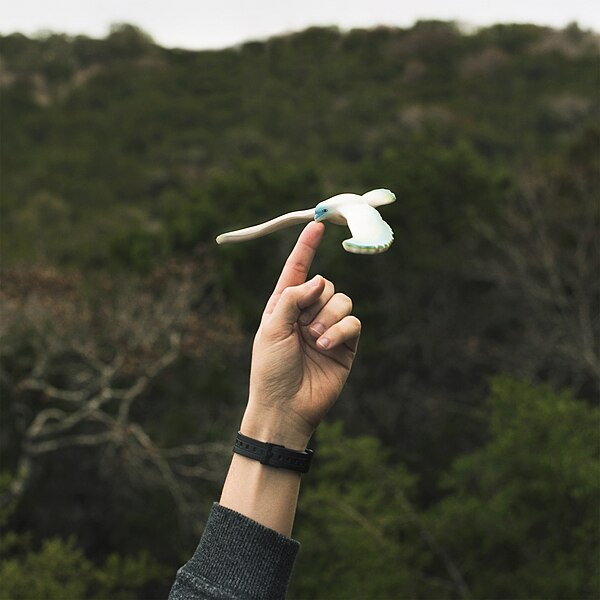
\includegraphics[width=0.4\textwidth]{chapters/chp4_pics/COG.jpg}
\caption{\textit{A balancing bird toy demonstrates the principle of center of mass. While often called the center of gravity, these terms are equivalent on Earth where gravitational field strength is approximately uniform. The bird's center of mass is carefully positioned below its support point (the beak) via a non-uniform density throughout the toy, creating a stable equilibrium. When disturbed, the bird will oscillate around this equilibrium point until returning to its stable position—a principle fundamental to both engineering design and physical analysis.}}
\label{fig:balance_bird}
\end{figure}


\exampleline
\begin{example}
A metal foundry is producing a cylindrical rod with a height of $L = 1$ meter and a radius of $R = 0.5$ meters. Due to the cooling process, the density of the rod varies with height according to $\rho(x,y,z) = k z^2$, where $z$ measures the height from the base of the cylinder. The total mass of the rod is measured to be $M = 10$ kg.

\begin{enumerate}
    \item Determine the value of the constant $k$ that describes the density distribution.
    \item Calculate the $z$-coordinate of the center of mass of the rod from the base.
\end{enumerate}

\begin{solution}
\begin{enumerate}
    \item \textbf{Determine $k$}: 

    The total mass of the rod is given by:
    \[
    M = \iiint_E \rho(x,y,z)\,dV.
    \]
    In cylindrical coordinates, $x^2 + y^2 = r^2$, and $dV = r\,dr\,d\theta\,dz$. The density becomes $\rho(r,\theta,z) = k z^2$, and the region $E$ is defined by $r \in [0, R]$, $\theta \in [0, 2\pi]$, and $z \in [0, L]$. Substituting:
    \[
    M = \int_0^L \int_0^{2\pi} \int_0^R k z^2 r \,dr\,d\theta\,dz.
    \]
    Separate the integrals:
    \[
    M = k \int_0^L z^2\,dz \int_0^{2\pi} d\theta \int_0^R r\,dr.
    \]
    Compute each integral:
    \[
    \int_0^{2\pi} d\theta = 2\pi, \quad \int_0^R r\,dr = \left[\frac{r^2}{2}\right]_0^R = \frac{R^2}{2}, \quad \int_0^L z^2\,dz = \left[\frac{z^3}{3}\right]_0^L = \frac{L^3}{3}.
    \]
    Substitute into the equation for $M$:
    \[
    M = k \cdot \frac{L^3}{3} \cdot 2\pi \cdot \frac{R^2}{2}.
    \]
    Simplify:
    \[
    M = k \cdot \frac{\pi R^2 L^3}{3}.
    \]
    Solve for $k$:
    \[
    k = \frac{3M}{\pi R^2 L^3}.
    \]
    Substitute $M = 10$, $R = 0.5$, and $L = 1$:
    \[
    k = \frac{3 \cdot 10}{\pi \cdot (0.5)^2 \cdot 1^3} = \frac{30}{\pi \cdot 0.25} = \frac{120}{\pi}.
    \]

    \item \textbf{Find the center of mass}: 

    The $z$-coordinate of the center of mass is:
    \[
    \bar{z} = \frac{1}{M} \iiint_E z \rho(x,y,z)\,dV.
    \]
    In cylindrical coordinates:
    \[
    \bar{z} = \frac{1}{M} \int_0^L \int_0^{2\pi} \int_0^R z (k z^2) r \,dr\,d\theta\,dz.
    \]
    Separate the integrals:
    \[
    \bar{z} = \frac{k}{M} \int_0^L z^3\,dz \int_0^{2\pi} d\theta \int_0^R r\,dr.
    \]
    Compute each integral:
    \[
    \int_0^{2\pi} d\theta = 2\pi, \quad \int_0^R r\,dr = \frac{R^2}{2}, \quad \int_0^L z^3\,dz = \left[\frac{z^4}{4}\right]_0^L = \frac{L^4}{4}.
    \]
    Substitute:
    \[
    \bar{z} = \frac{k}{M} \cdot \frac{L^4}{4} \cdot 2\pi \cdot \frac{R^2}{2}.
    \]
    Simplify:
    \[
    \bar{z} = \frac{k \pi R^2 L^4}{4M}.
    \]
    Substituting $k = \frac{120}{\pi}$, $M = 10$, $R = 0.5$, and $L = 1$:
    \[
    \bar{z} = \frac{\frac{120}{\pi} \cdot \pi \cdot (0.5)^2 \cdot 1^4}{4 \cdot 10}.
    \]
    Simplify:
    \[
    \bar{z} = \frac{120 \cdot 0.25}{40} = \frac{30}{40} = 0.75 \, \text{meters}.
    \]

    \noindent The center of mass of the rod is located $0.75$ meters from the base.
\end{enumerate}
\end{solution}
\end{example}
\exampleline


\subsection*{Moments and Products of Inertia in Three Dimensions} \index{Moment of Inertia} \index{Product of Inertia}

\noindent When an object rotates, its resistance to changes in rotational motion depends not just on its total mass but on how that mass is distributed. Think of a figure skater pulling in their arms to spin faster, or a diver tucking into a ball to increase their rotation speed. These effects are described by quantities called moments and products of inertia. \\

\noindent For rotation about the coordinate axes, we define the moments of inertia:
\begin{align*}
I_x &= \iiint_E (y^2 + z^2)\rho(x,y,z)\,dV \\
I_y &= \iiint_E (x^2 + z^2)\rho(x,y,z)\,dV \\
I_z &= \iiint_E (x^2 + y^2)\rho(x,y,z)\,dV
\end{align*}

\noindent Each moment measures how hard it is to rotate the object about that axis. Notice the squared terms - mass farther from the axis contributes more to the moment of inertia, just as it's harder to spin a dumbbell held at arm's length than one held close to your body. \\

\noindent The products of inertia capture how rotation about one axis affects rotation about others:
\begin{align*}
I_{xy} &= \iiint_E xy\rho(x,y,z)\,dV \\
I_{yz} &= \iiint_E yz\rho(x,y,z)\,dV \\
I_{xz} &= \iiint_E xz\rho(x,y,z)\,dV
\end{align*}
\index{Tensors}
\noindent This distribution is characterized by moments and products of inertia that we can arrange in a special $3 \times 3$ grid called the inertia tensor:
\[
\begin{bmatrix}
I_{xx} & -I_{xy} & -I_{xz} \\
-I_{yx} & I_{yy} & -I_{yz} \\
-I_{zx} & -I_{zy} & I_{zz}
\end{bmatrix}
\]

\noindent Though this appears as a matrix (a 2-dimensional array of numbers), it represents something more fundamental in physics. Just as vectors (1-dimensional arrays) are special cases of matrices, matrices themselves are special cases of tensors - mathematical objects that preserve relationships between physical quantities regardless of how we measure them. Consider a spinning top - its rotational behavior remains the same whether we measure it using $xyz$ coordinates or any other system. The inertia tensor $\mathbf{I}$ captures this fundamental behavior by relating angular velocity to angular momentum in a way that remains true under any coordinate transformation. While the mathematics of tensors extends beyond this text, we can work with $\mathbf{I}$ as a matrix while appreciating its deeper physical significance. \\

\noindent This structure explains why there exist three special directions called principal axes where rotation is simplest - imagine spinning a book along its length, width, or thickness. When rotating about these axes, the object spins cleanly without wobbling. While finding these directions involves concepts from linear algebra that we'll encounter in later courses, understanding their existence helps explain why gymnasts and divers choose particular axes for their rotations.\\

\noindent These physical insights manifest in several fundamental equations. For any rotating object in 3D space, with angular velocity $\boldsymbol{\omega} = (\omega_x, \omega_y, \omega_z)$ and angular acceleration $\boldsymbol{\alpha} = (\alpha_x, \alpha_y, \alpha_z)$, we can describe its motion using the inertia tensor:

\begin{itemize} \index{Angular Momentum}
   \item Angular momentum:
   \[
   \begin{bmatrix} L_x \\ L_y \\ L_z \end{bmatrix} = 
   \begin{bmatrix}
   I_{xx} & -I_{xy} & -I_{xz} \\
   -I_{yx} & I_{yy} & -I_{yz} \\
   -I_{zx} & -I_{zy} & I_{zz}
   \end{bmatrix}
   \begin{bmatrix} \omega_x \\ \omega_y \\ \omega_z \end{bmatrix}
   \]
   
   \item Rotational kinetic energy: \index{Rotational Motion}
   \[
   E = \frac{1}{2}\begin{bmatrix} \omega_x & \omega_y & \omega_z \end{bmatrix}
   \begin{bmatrix}
   I_{xx} & -I_{xy} & -I_{xz} \\
   -I_{yx} & I_{yy} & -I_{yz} \\
   -I_{zx} & -I_{zy} & I_{zz}
   \end{bmatrix}
   \begin{bmatrix} \omega_x \\ \omega_y \\ \omega_z \end{bmatrix}
   \]
   
   \item Torque: \index{Torque}
   \[
   \begin{bmatrix} \tau_x \\ \tau_y \\ \tau_z \end{bmatrix} = 
   \begin{bmatrix}
   I_{xx} & -I_{xy} & -I_{xz} \\
   -I_{yx} & I_{yy} & -I_{yz} \\
   -I_{zx} & -I_{zy} & I_{zz}
   \end{bmatrix}
   \begin{bmatrix} \alpha_x \\ \alpha_y \\ \alpha_z \end{bmatrix}
   \]
\end{itemize}

\noindent When an object is symmetric or rotates about a principal axis, the off-diagonal terms ($I_{xy}, I_{yz}, I_{xz}$) become zero and these equations simplify to the scalar forms seen earlier. Common examples include a cylinder spinning about its axis or a sphere rotating about any diameter. \\

\noindent These matrix operations work as follows: \\

\noindent \textbf{Matrix-Vector Multiplication:} \index{Matrix Operations} When multiplying a $3 \times 3$ matrix by a $3 \times 1$ vector:
\[
\begin{bmatrix}
a & b & c \\
d & e & f \\
g & h & i
\end{bmatrix}
\begin{bmatrix}
x \\ y \\ z
\end{bmatrix}
=
\begin{bmatrix}
ax + by + cz \\
dx + ey + fz \\
gx + hy + iz
\end{bmatrix}
\]

\noindent \textbf{Vector-Matrix-Vector Multiplication:} For a row vector times matrix times column vector:
\[
\begin{bmatrix} x & y & z \end{bmatrix}
\begin{bmatrix}
a & b & c \\
d & e & f \\
g & h & i
\end{bmatrix}
\begin{bmatrix} x \\ y \\ z \end{bmatrix}
= ax^2 + (b+d)xy + (c+g)xz + (e)y^2 + (f+h)yz + (i)z^2
\]

\noindent This explains why the kinetic energy expression $E = \frac{1}{2}\boldsymbol{\omega}^T\mathbf{I}\boldsymbol{\omega}$ produces a scalar value - it's a vector-matrix-vector product that combines all the moments and products of inertia with the angular velocity components. The $T$ over $\boldsymbol{\omega}$ represents the \textit{transpose} which switches the component indices, i.e., $x_{ij}$ becomes $x_{ji}$. Note that this can also change the structure, especially seen in the kinetic energy expression where the dimensions of $\boldsymbol{\omega}$ are $3 \times 1$ where $\boldsymbol{\omega}^T$ has dimensions $1 \times 3$ which are not the same and have different structural meanings.

%https://commons.wikimedia.org/wiki/File:Matrix_multiplication_qtl1.svg
\begin{figure}[H]
\centering
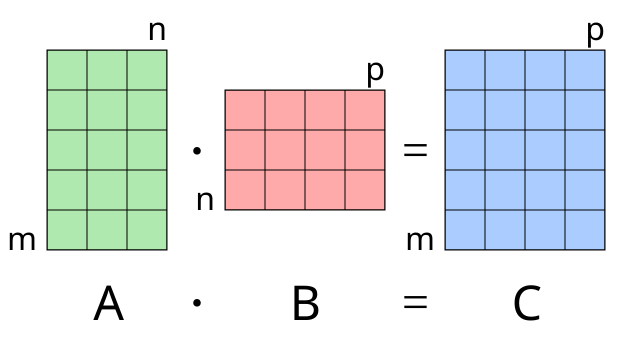
\includegraphics[width=0.4\textwidth]{chapters/chp4_pics/matrix.png}
\caption{\textit{A visualization of matrix operations. Notice the change in dimensionality. For any matrix multiplication we will have $A_{m\times n} \cdot B_{n \times p} = C_{m \times p}$. Note that the column dimension of $A$ must equal the row dimension of $B$ or else you cannot perform the matrix operation}}
\label{fig:matrix}
\end{figure}

\noindent Matrices naturally emerge in multivariate calculus as they elegantly encode how quantities in multiple dimensions relate to and transform each other, just as we've seen with moments of inertia describing rotational motion. While we've only scratched the surface here, a deeper study of linear algebra reveals powerful tools for understanding everything from coordinate transformations to optimization problems in higher dimensions. As you continue your mathematical journey, we strongly encourage exploring linear algebra to gain deeper insight into the beautiful structures underlying multivariate calculus.

\subsection*{Force and Work in Space}

\noindent When a force varies continuously throughout a region of space, triple integrals help us calculate its effects. Consider a force field $\mathbf{F}(x,y,z)$ acting on a solid object. Just as with mass distribution, we can integrate the components of the force field over the region to find the total force exerted on the object in each direction:
\begin{align*}
F_x &= \iiint_E F_x(x,y,z)\,dV, \\
F_y &= \iiint_E F_y(x,y,z)\,dV, \\
F_z &= \iiint_E F_z(x,y,z)\,dV.
\end{align*}

\noindent Work---the energy transferred by a force acting over a displacement---is most naturally computed along a specific path using a \textit{line integral}, which we will develop fully in Chapter 5. For now, we focus on what triple integrals \textit{can} tell us: the \textbf{total instantaneous power} exerted on a distributed body.\\ \\
\noindent When a force field \( \mathbf{F}(x,y,z) \) acts on a body whose points move with velocity field \( \mathbf{v}(x,y,z) \), the \textit{power density} (rate of doing work per unit volume) at each point is:
\[
P(x,y,z) = \mathbf{F}(x,y,z) \cdot \mathbf{v}(x,y,z).
\]
The total instantaneous power delivered to the body is then:
\[
\mathcal{P}_{\text{total}} = \iiint_E \mathbf{F}(x,y,z) \cdot \mathbf{v}(x,y,z) \, dV.
\]
\noindent To find the actual \textit{work} (energy) delivered over a time interval, one would integrate the total power over time: \( W = \int_0^T \mathcal{P}_{\text{total}}(t) \, dt \). We will see more direct approaches to computing work in Chapter 5.

\noindent This framework is essential in physics and engineering applications. For example, when calculating the work done by an electric field $\mathbf{E}$ on a charge distribution $\rho(x,y,z)$ moving with velocity $\mathbf{v}(x,y,z)$, the integral takes the form:
\[
W = \iiint_E \rho(x,y,z)\bigl(\mathbf{E} \cdot \mathbf{v}\bigr)\,dV,
\]
where $\mathbf{v}$ is the local velocity vector at each point in the charge distribution. Here, the triple integral sums contributions to the total work throughout the entire region of charge. This process models how electric forces interact with volumetric charge distributions in systems such as capacitors or plasma clouds. \\

\noindent In Chapter 5, we will refine these concepts further by introducing line integrals and exploring how work is more directly computed along specific paths within a vector field. For now, understand that triple integrals are invaluable for modeling distributed forces and power densities across volumes.

\exampleline
\begin{example}
A magnetic field $\mathbf{B}(x,y,z) = (y^2, xz, xy)$ tesla acts on a conductive fluid in the unit cube $[0,1]^3$. The fluid has charge density $\rho(x,y,z) = e^{-(x^2 + y^2 + z^2)}  \text{(coulombs/m$^3$)}$ and velocity $\mathbf{v}(x,y,z) = (z, x, y) \quad \text{(m/s)}$. \\

\noindent Find:
\begin{enumerate}
   \item The total magnetic force on the fluid given the differential Lorentz force $d\mathbf{F} =  \rho(\mathbf{r}) \bigl(\mathbf{v} \times \mathbf{B}\bigr)\,dV$ and force density $\mathbf{f}(\mathbf{r}) = \rho(\mathbf{r})\,[\,\mathbf{v}(\mathbf{r}) \times \mathbf{B}(\mathbf{r})\,]$
   \item The work done by the magnetic field in one second, given that instantaneous power is $dP = \mathbf{F}\cdot\mathbf{v}$
\end{enumerate}

\begin{solution}
\begin{enumerate}
   \item \textbf{Total Magnetic Force on the Fluid} \\
   
   Computing the cross product:
   \[
   \mathbf{v} \times \mathbf{B}
   =
   \begin{vmatrix}
   \mathbf{i} & \mathbf{j} & \mathbf{k}\\
   z & x & y\\
   y^2 & xz & xy
   \end{vmatrix}
   =
   \bigl(x^2y - xyz,\;\;y^3 - xyz,\;\;xz^2 - xy^2\bigr)
   \]
   
   Hence the total force components are:
   \begin{align*}
   F_x &= \iiint_{E=[0,1]^3} e^{-(x^2 + y^2 + z^2)}\,(x^2y - x y z)\, dV \\[1ex]
   F_y &= \iiint_{E=[0,1]^3} e^{-(x^2 + y^2 + z^2)}\,(y^3 - x y z)\, dV \\[1ex]
   F_z &= \iiint_{E=[0,1]^3} e^{-(x^2 + y^2 + z^2)}\,(x z^2 - x y^2)\, dV
   \end{align*}

   \item \textbf{Work Done by the Magnetic Field in One Second} \\
   
   For a fluid element, the differential power is:
   \[
   dP = \bigl[\rho(\mathbf{v}\times\mathbf{B})\bigr]\cdot\mathbf{v}\,dV 
   \;=\; \rho \bigl(\mathbf{v}\times\mathbf{B}\bigr)\cdot \mathbf{v}\, dV
   \]
   
   Because $\mathbf{v}\times\mathbf{B}$ is always perpendicular to $\mathbf{v}$, their dot product is zero:
   \[
   (\mathbf{v}\times\mathbf{B})\cdot\mathbf{v} = 0
   \]
   
   Thus the magnetic field does no work on the fluid:
   \[
   W = \iiint_{E} \rho \bigl[(\mathbf{v}\times\mathbf{B})\cdot\mathbf{v}\bigr]\; dV = 0
   \]
\end{enumerate}

\end{solution}
\end{example}
\exampleline
\begin{example}
A force field $\mathbf{F}(x,y,z) = (yz, xz, xy)$ newtons acts on a volume of gas expanding in the unit cube $[0,1]^3$. The gas particles move with velocity
\[
\mathbf{v}(x,y,z) = (x, y, z) \quad \text{(m/s)}.
\]
Find:
\begin{enumerate}
   \item The total force on the gas volume
   \item The work done by the force field on the gas, given that instantaneous power is $dP = \mathbf{F}\cdot\mathbf{v}\,dV$
\end{enumerate}

\begin{solution}
\begin{enumerate}
   \item \textbf{Total Force Components} \\
   
   The total force is found by integrating each component over the volume:
   \begin{align*}
   F_x &= \iiint_{[0,1]^3} yz\,dV = \int_0^1\int_0^1\int_0^1 yz\,dx\,dy\,dz \\
   &= \int_0^1\int_0^1 yz\,dy\,dz = \int_0^1 \frac{z}{2}\,dz = \frac{1}{4} \\[2ex]
   F_y &= \iiint_{[0,1]^3} xz\,dV = \int_0^1\int_0^1\int_0^1 xz\,dx\,dy\,dz \\
   &= \int_0^1\int_0^1 \frac{z}{2}\,dy\,dz = \frac{1}{4} \\[2ex]
   F_z &= \iiint_{[0,1]^3} xy\,dV = \int_0^1\int_0^1\int_0^1 xy\,dx\,dy\,dz \\
   &= \int_0^1\int_0^1 \frac{y}{2}\,dy\,dz = \frac{1}{4}
   \end{align*}
   
   Therefore $\mathbf{F}_{total} = (\frac{1}{4}, \frac{1}{4}, \frac{1}{4})$ newtons.

   \item \textbf{Work Done by the Force Field} \\
   
   The instantaneous power at each point is:
   \begin{align*}
   \mathbf{F}\cdot\mathbf{v} &= (yz, xz, xy)\cdot(x, y, z) \\
   &= xyz + xyz + xyz \\
   &= 3xyz
   \end{align*}
   
   Therefore the total work done is:
   \begin{align*}
   W &= \iiint_{[0,1]^3} 3xyz\,dV \\
   &= 3\int_0^1\int_0^1\int_0^1 xyz\,dx\,dy\,dz \\
   &= 3\int_0^1\int_0^1 \frac{y}{2}z\,dy\,dz \\
   &= 3\int_0^1 \frac{z}{4}\,dz = \frac{3}{8} \text{ joules}
   \end{align*}
\end{enumerate}
\end{solution}
\end{example}
\exampleline

\subsection*{Average Values and Distributions} \index{Average Value} \index{Average Distribution}

\noindent Just as we found average values using double integrals, we can find the average value of a function $f(x,y,z)$ over a three-dimensional region $E$:
\[
f_{avg} = \frac{\iiint_E f(x,y,z)\,dV}{\iiint_E dV}
\]

\noindent This concept proves invaluable in various physical contexts:
\begin{itemize}
\item Temperature distribution in a solid body, where $f(x,y,z)$ represents temperature
\item Concentration of a solute in a solution, where $f(x,y,z)$ gives concentration
\item Stress distribution in a structural element, where $f(x,y,z)$ describes stress intensity
\end{itemize}

\noindent The denominator $\iiint_E dV$ represents the volume of region $E$, making this formula a natural extension of the average value theorem to three dimensions. When working with non-uniform materials, we often need weighted averages that account for varying density:
\[
f_{avg} = \frac{\iiint_E f(x,y,z)\rho(x,y,z)\,dV}{\iiint_E \rho(x,y,z)\,dV}
\]

\noindent This weighted form finds particular use in materials science and engineering, where we might need to account for how material properties vary throughout a component. For instance, in a composite material, both density and thermal conductivity might vary spatially, affecting the overall thermal behavior of the object.


\exampleline
\begin{example}
A spherical blast furnace of radius 3 meters operates at extremely high temperatures. The temperature (in Celsius) at any point $(x,y,z)$ in the furnace varies according to:
\[
T(x,y,z) = 1500e^{-(x^2+y^2+z^2)/9} + 500
\]
The density of the gas inside the furnace varies with height according to:
\[
\rho(x,y,z) = e^{-z/3} \quad \text{(kg/m}^3\text{)}
\]
Find:
\begin{enumerate}
   \item The average temperature in the furnace
   \item The density-weighted average temperature, accounting for the fact that hotter regions tend to have different densities
\end{enumerate}

\begin{solution}
\begin{enumerate}
   \item First, note the volume of our region $E$, a sphere of radius 3:
   \[
   \iiint_E dV = \frac{4}{3}\pi(3^3) = 36\pi
   \]
   The average temperature is:
   \[
   T_{\mathrm{avg}} = \frac{\iiint_E T(x,y,z)\,dV}{\iiint_E dV} = \frac{\iiint_E T(x,y,z)\,dV}{36\pi}
   \]
   Converting to spherical coordinates $\bigl(r,\phi,\theta\bigr)$ with 
   \[
   x = r\sin\phi\cos\theta,\quad
   y = r\sin\phi\sin\theta,\quad
   z = r\cos\phi,\quad
   dV = r^2\sin\phi\,dr\,d\phi\,d\theta,
   \]
   we have $x^2 + y^2 + z^2 = r^2$, so the temperature becomes
   \[
   T(r) = 1500\,e^{-\tfrac{r^2}{9}} + 500.
   \]
   Therefore,
   \[
   \iiint_E T(x,y,z)\,dV 
   = \int_0^{2\pi}\!\int_0^{\pi}\!\int_0^3 \Bigl(1500\,e^{-\tfrac{r^2}{9}} + 500\Bigr)\,r^2\sin\phi\,dr\,d\phi\,d\theta.
   \]
   The angular parts give a factor of $4\pi$, so
   \[
   \iiint_E T(x,y,z)\,dV 
   = 4\pi\Bigl[
      1500\int_0^3 r^2 e^{-\tfrac{r^2}{9}}\,dr
      + 500\int_0^3 r^2\,dr
   \Bigr].
   \]
   Evaluating,
   \[
   \int_0^3 r^2\,dr = 9
   \quad\text{and}\quad
   \int_0^3 r^2 e^{-\tfrac{r^2}{9}}\,dr \approx 5.12.
   \]
   Hence,
   \[
   1500 \cdot 5.12 + 500 \cdot 9
   = 7680 + 4500
   = 12180.
   \]
   Multiplying by $4\pi$ gives:
   \[
   12180 \cdot 4\pi = 48720\pi.
   \]
   So
   \[
   T_{\mathrm{avg}} 
   = \frac{48720\pi}{36\pi} 
   \approx 1353\;\text{°C}.
   \]

   \item The density-weighted average temperature is
   \[
   T_{\mathrm{avg}} 
   = \frac{\iiint_E T(x,y,z)\,\rho(x,y,z)\,dV}
          {\iiint_E \rho(x,y,z)\,dV}.
   \]
   In spherical coordinates, $z = r\cos\phi$, so
   \[
   \rho(r,\phi) = e^{-\tfrac{r\cos\phi}{3}}.
   \]
   The resulting integrals involve products of exponentials in $r$ and $\cos\phi$, so we evaluate them numerically using programming or Wolfram Alpha. One finds
   \[
   T_{\mathrm{avg}} \approx 1280\;\text{°C}.
   \]
\end{enumerate}
\vspace{0.5em}
\noindent
The density-weighted average is lower because the hotter central regions (larger $r^2$ term in $e^{-r^2/9}$) coincide with regions where $\rho$ is relatively smaller for higher $z$; effectively, less ``weight” is assigned to the hottest points.
\end{solution}
\end{example}
\exampleline



\newpage

\formsdefs{}

\subsection*{Important Vocabulary}
\begin{itemize}
\item \textbf{Double Integral:} A mathematical tool that measures accumulation over a two-dimensional region, used to find quantities like area, volume, mass, and center of mass.

\item \textbf{Double Integral Type I Region:} A region \(R\) in the \((x,y)\)-plane of the form \(R = \{(x,y) : a \leq x \leq b, g_1(x) \leq y \leq g_2(x)\}\), where vertical lines intersect the region's boundary exactly twice.

\item \textbf{Double Integral Type II Region:} A region \(R\) in the \((x,y)\)-plane of the form \(R = \{(x,y) : c \leq y \leq d, h_1(y) \leq x \leq h_2(y)\}\), where horizontal lines intersect the region's boundary exactly twice.

\item \textbf{Fubini's Theorem:} States that a double or triple integral can be evaluated as repeated integrals in any order over a rectangular region.

\item \textbf{Triple Integral:} An extension of double integrals to three dimensions, used to find volumes, mass, and other physical quantities in \(\mathbb{R}^3\).

\item \textbf{Triple Integral Type I Region:} A solid region \(E\) bounded above and below by surfaces \(z = g_2(x,y)\) and \(z = g_1(x,y)\) over a region \(R\) in the \((x,y)\)-plane, where vertical lines intersect the boundary exactly twice.

\item \textbf{Triple Integral Type II Region:} A solid region \(E\) bounded by surfaces \(x = h_1(y,z)\) and \(x = h_2(y,z)\) over a region \(R\) in the \((y,z)\)-plane, where lines parallel to the \(x\)-axis intersect the boundary exactly twice.

\item \textbf{Triple Integral Type III Region:} A solid region \(E\) bounded by surfaces \(y = k_1(x,z)\) and \(y = k_2(x,z)\) over a region \(R\) in the \((x,z)\)-plane, where lines parallel to the \(y\)-axis intersect the boundary exactly twice.

\item \textbf{Jacobian Determinant:} A measure of how a coordinate transformation affects area or volume elements, denoted \(|J|\).

\item \textbf{Moment of Inertia:} A measure of an object's resistance to rotational motion about an axis, denoted \(I_x\), \(I_y\), or \(I_z\).

\item \textbf{Product of Inertia:} A measure of coupling between rotations about different axes, denoted \(I_{xy}\), \(I_{yz}\), or \(I_{xz}\).

\item \textbf{Center of Mass:} The point \((\bar{x}, \bar{y}, \bar{z})\) where an object's mass can be considered concentrated for certain calculations.

\item \textbf{Inertia Tensor:} A \(3\times3\) matrix describing how mass is distributed in a rotating object.

\item \textbf{Iterated Integral:} A multiple integral evaluated as a sequence of single integrals, integrating one variable at a time while treating the others as constants.

\item \textbf{Polar Coordinates:} A coordinate system \( (r, \theta) \) where \( r \) is the distance from the origin and \( \theta \) is the angle from the positive \( x \)-axis. The area element is \( dA = r \, dr \, d\theta \).

\item \textbf{Cylindrical Coordinates:} A coordinate system \( (r, \theta, z) \) extending polar coordinates by adding a height \( z \). The volume element is \( dV = r \, dr \, d\theta \, dz \).

\item \textbf{Spherical Coordinates:} A coordinate system \( (\rho, \theta, \phi) \) where \( \rho \) is the distance from the origin, \( \theta \) is the azimuthal angle, and \( \phi \) is the polar angle from the \( z \)-axis. The volume element is \( dV = \rho^2 \sin\phi \, d\rho \, d\theta \, d\phi \).

\item \textbf{Change of Variables:} A technique for simplifying integrals by substituting new coordinate variables, requiring multiplication by the absolute value of the Jacobian determinant.

\item \textbf{Surface Area:} The area of a surface \( z = f(x,y) \) over a region \( R \), computed as \( \iint_R \sqrt{1 + f_x^2 + f_y^2} \, dA \).
\end{itemize}

\subsection*{Key Formulas}
\begin{multicols}{2}

\paragraph{Fubini's Theorem (Rectangular)}
\[
\iint_R f\,dA = \int_a^b\!\int_c^d f(x,y)\,dy\,dx = \int_c^d\!\int_a^b f(x,y)\,dx\,dy
\]

\paragraph{Type I Region (vertical slicing)}
\[
\iint_R f\,dA = \int_a^b\!\int_{g_1(x)}^{g_2(x)} f(x,y)\,dy\,dx
\]

\paragraph{Type II Region (horizontal slicing)}
\[
\iint_R f\,dA = \int_c^d\!\int_{h_1(y)}^{h_2(y)} f(x,y)\,dx\,dy
\]

\paragraph{Polar Coordinates}
\begin{align*}
x &= r\cos\theta, \quad y = r\sin\theta \\
dA &= r\,dr\,d\theta
\end{align*}
\[
\iint_R f\,dA = \int_\alpha^\beta\!\int_{r_1(\theta)}^{r_2(\theta)} f(r\cos\theta,r\sin\theta)\,r\,dr\,d\theta
\]

\paragraph{Area and Volume}
\[
\text{Area} = \iint_R 1\,dA \qquad \text{Volume} = \iiint_E 1\,dV
\]

\paragraph{Surface Area ($z = g(x,y)$)}
\[
A = \iint_R \sqrt{1 + g_x^2 + g_y^2}\,dA
\]

\paragraph{Mass, Moments, Center of Mass (2D)}
\begin{align*}
M &= \iint_R \rho\,dA \\
M_x &= \iint_R y\,\rho\,dA, \quad M_y = \iint_R x\,\rho\,dA \\
\bar{x} &= M_y/M, \quad \bar{y} = M_x/M
\end{align*}

\paragraph{2D Moments of Inertia}
\begin{align*}
I_x &= \iint_R y^2\rho\,dA, \quad I_y = \iint_R x^2\rho\,dA \\
I_0 &= I_x + I_y = \iint_R (x^2+y^2)\rho\,dA
\end{align*}

\paragraph{Average Value}
\[
f_{\text{avg}} = \frac{\iint_R f\,dA}{\iint_R dA} \qquad \text{(similarly for triple integrals)}
\]

\paragraph{Triple Integrals}
\begin{align*}
M &= \iiint_E \rho\,dV \\
\bar{x} &= \frac{1}{M}\iiint_E x\rho\,dV, \;\;\text{etc.}
\end{align*}

\paragraph{Cylindrical Coordinates}
\begin{align*}
x &= r\cos\theta, \quad y = r\sin\theta, \quad z = z \\
dV &= r\,dr\,d\theta\,dz
\end{align*}

\paragraph{Spherical Coordinates}
\begin{align*}
x &= \rho\sin\phi\cos\theta, \quad y = \rho\sin\phi\sin\theta \\
z &= \rho\cos\phi \\
dV &= \rho^2\sin\phi\,d\rho\,d\phi\,d\theta
\end{align*}

\paragraph{3D Moments of Inertia}
\begin{align*}
I_x &= \iiint_E (y^2+z^2)\rho\,dV \\
I_y &= \iiint_E (x^2+z^2)\rho\,dV \\
I_z &= \iiint_E (x^2+y^2)\rho\,dV
\end{align*}

\paragraph{Jacobian and Change of Variables}
\[
|J| = \left|\frac{\partial(x,y)}{\partial(u,v)}\right| = \left|\det\begin{bmatrix} x_u & x_v \\ y_u & y_v \end{bmatrix}\right|
\]
\[
\iint_R f(x,y)\,dA = \iint_{R'} f(x(u,v),y(u,v))\,|J|\,du\,dv
\]
Triple integral version: $dV = |J|\,du\,dv\,dw$ with $3\times 3$ determinant.

\paragraph{Common Jacobians}
\begin{align*}
\text{Polar:}\quad |J| &= r \\
\text{Cylindrical:}\quad |J| &= r \\
\text{Spherical:}\quad |J| &= \rho^2\sin\phi
\end{align*}

\end{multicols}



\newpage


\practice{}

\begin{multicols}{2}

\begin{enumerate}
%lecture 1

\item Evaluate \(\displaystyle\iint_R (2x + 3y)\,dA\) where \(R = [0,2] \times [1,3]\).

\item Find \(\displaystyle\iint_R xy^2\,dA\) where \(R = [-1,1] \times [0,2]\).


\item Calculate \(\displaystyle\iint_R \sin(x+y)\,dA\) where \(R = [0,\pi] \times [0,\pi]\).

\item Consider a rectangular sheet \([0,a] \times [0,b]\) with temperature distribution \(T(x,y) = \sin(\pi x/a)\sin(\pi y/b)\). Find its average temperature.

\item The force on an electrical conductor depends on position according to \(F(x,y) = Be^{-x^2-y^2}\) newtons per square meter, where \(B\) is magnetic field strength. Find the total force on a rectangular conductor \([-1,1] \times [-1,1]\) when \(B = 2\).

\item If \( f(x,y) = ax + b \) on \( R = [0,1] \times [0,1] \) with \( \iint_R f \, dA = 4 \) and \( \iint_R x f \, dA = 3 \), find \( a \) and \( b \), then compute \( \iint_R x^2 f \, dA \).

\item Evaluate \(\displaystyle\iint_R \frac{1}{(1+x^2)(1+y^2)}\,dA\) where \(R = [0,1] \times [0,1]\).

\item 
Use a Riemann sum to approximate
\[
\iint_{[0,2]\times[1,3]} 2x y \, dA
\]
by dividing both dimensions into \(2\) equal parts (a \(2 \times 2\) grid). Take the \emph{midpoint} of each subrectangle as the sample point. Show the subdivision, identify each sample point, and compute the resulting sum. Do \emph{not} convert this into an iterated integral directly; follow the Riemann sum framework:
\[
S_{2,2} = \sum_{i=1}^2 \sum_{j=1}^2 f(x_{ij}^*, y_{ij}^*)\,\Delta A.
\]

\item 
Consider the function \(f(x,y) = x - y\) over the rectangular region \(\,[0,1]\times[0,2]\,.\)
\begin{enumerate}
   \item Set up \(\iint_R (x - y)\,dA\) explicitly as an iterated integral.
   \item Evaluate the integral and interpret the result in terms of \emph{negative} and \emph{positive} volume, given that \(x-y\) dips below the \(xy\)-plane in some parts of \(R\).
\end{enumerate}

\item
Evaluate using Fubini’s Theorem:
\[
\iint_{R} \bigl(3 + 2x\bigr)\, dA,
\]
where \(R = [1,2]\times[0,1]\). Show both orders of integration explicitly and confirm they produce the same numerical result.

\item
Let \(f(x,y)= e^x \sin(y)\). Compute
\[
\iint_{[0,\pi]\times[-1,1]} e^x \sin(y)\,dA
\]
by factoring the integral into a product of two single-variable integrals. Show each step clearly.

\item 
Determine which order of integration is simpler, and then evaluate:
\[
\iint_{[0,1]\times[2,3]} \frac{x}{1 + x^2 + y^2} \, dA.
\]
Discuss briefly why integrating with respect to \(y\) first (or vice versa) might be advantageous. Verify the final result.

\item 
Consider
\[
\iint_{[1,2]\times[0,2]} \frac{1}{(x+1)(y+2)} \,dA.
\]
\begin{enumerate}
   \item Rewrite the integrand using partial fractions if helpful.
   \item Evaluate the resulting iterated integral using Fubini’s Theorem.
\end{enumerate}

\item 
Briefly explain why the choice of sample points (lower-left, upper-right, midpoint, or max/min) does not affect the \emph{limit} of the Riemann sum for a \emph{continuous} function over a rectangular region. In your explanation, address how increasing the partition’s fineness guarantees convergence to a single value. (No detailed calculations required; this is conceptual.)

\item 
Show that
\[
\iint_{[-1,1]\times[-2,2]} \frac{xy}{x^2 + y^2}\,dA = 0
\]
by leveraging symmetry arguments rather than brute-force integration. Hint: For fixed \(x\), consider the integrand’s behavior as \(y\) varies symmetrically around \(0\).

(Note: the integrand has a removable singularity at the origin since \( |xy/(x^2+y^2)| \leq 1/2 \), so the integral converges.)

\item 
Recall that the average value of \(f(x,y)\) over \(R\) is  
\[
f_{\text{avg}} \;=\; \frac{1}{\text{Area}(R)} \,\iint_R f(x,y)\,dA.
\]
Compute the average value of \(f(x,y) = \sin(xy)\) over \(R = [0,2]\times[0,2]\). Then simplify your final expression if possible.

\item 
Find the general form of the indefinite double integral:
\[
\iint x^2 y \,dx\,dy.
\]
Explicitly show how you introduce an arbitrary function of one variable at each step.

\item 
Compute the indefinite double integral:
\[
\iint \bigl( 3x + 2xy^2 \bigr)\,dx\,dy,
\]
carefully indicating the arbitrary functions that arise. Provide your final answer as
\[
F(x,y) + g(x) + h(y).
\]

    \item Show that for any continuous function \(f(x,y)\) on \([a,b] \times [c,d]\):
    \begin{multline*}
        \iint_R f(x,y)\,dA = \frac{(b-a)(d-c)}{4}  \\
        \big[f(a,c) + f(a,d) + f(b,c) + f(b,d)\big]
    \end{multline*}
    if and only if \(f(x,y)\) is bilinear (linear in each variable and of the form $f(x,y) = \alpha x + \beta y + \gamma xy + \delta$).

\item Prove the Cauchy-Schwarz inequality for double integrals: if \(f\) and \(g\) are continuous on \(R\), then
    \begin{multline*}
\left(\iint_R f \, g \, dA\right)^{\!2} \\
\leq \left(\iint_R f^2 \, dA\right)\!\left(\iint_R g^2 \, dA\right).
    \end{multline*}
    \textit{Hint:} Consider \(\iint_R (f + tg)^2 \, dA \geq 0\) for all \(t \in \mathbb{R}\) and examine the discriminant.

\item For a quantum particle in a box \([0,a] \times [0,b]\), the probability density is:
\[
|\psi(x,y)|^2 = \frac{4}{ab}\sin^2(\frac{\pi x}{a})\sin^2(\frac{\pi y}{b})
\]
Show that the total probability equals 1.

%lecture 2
\item Sketch the region bounded below by $y=0$ and above by $y=3x$ for $0 \le x \le 2$. Write down (but do not evaluate) the double integral
\[
\iint_R (x + y)\, dA
\]
as a Type I region, stating all limits clearly.

\item Consider the region $R$ bounded on the left by $x=1$ and on the right by $x = y + 3$, with $-2 \le y \le 2$. Express
\[
\iint_R 5\,dA
\]
as a Type II double integral, but do not integrate. Show the bounds for $y$ and $x$ explicitly.

\item A region $R$ is described by $0 \le x \le 4$ and $x^2 \le y \le 8 + x$.  
\begin{enumerate}
\item Explain why $R$ is Type I in $x$.  
\item Attempt to describe the same $R$ as Type II: find the interval for $y$ and the functions $h_1(y)$, $h_2(y)$.
\end{enumerate}
No need to integrate; just show the correct bounds for each description.

\item Find the area of the region bounded by $y = x^2$ and $y = 6 - x$ for $-1 \le x \le 3$. Write and evaluate
\[
\iint_R 1 \,dA.
\]
If necessary, split into subregions to handle where the curves intersect.

\item Let $R$ be the region with $0 \le x \le 2$ and $x \le y \le 4$. Evaluate
\[
\iint_R (1 + xy)\, dA
\]
using:  
\begin{enumerate}
\item Type I bounds in the order $dy\,dx$,  
\item Type II bounds in the order $dx\,dy$.  
Confirm both give the same result.
\end{enumerate}

\item A region $R$ in the plane is bounded by $x=0$, $y=-2$, $y=2$, and $x = (y+1)^2$. Compute
\[
\iint_R \bigl(4 - x - y\bigr)\, dA
\]
using a Type II setup. First, identify $h_1(y)$ and $h_2(y)$, then integrate.

\item Use polar coordinates to evaluate the double integral
\[
\iint_R \bigl(x^2 + y^2\bigr)\, dA
\]
where $R$ is the disk of radius $3$ centered at the origin. Clearly indicate the $r$ and $\theta$ bounds.

\item Set up (but do not evaluate) the double integral for
\[
\iint_R (x^2 + y^2) \, dA
\]
over the sector where $0 \le r \le 2$, $\frac{\pi}{4} \le \theta \le \frac{3\pi}{4}$. Show each step of your conversion to polar form.

\item Compute
\[
\iint_R \bigl(3 + x + y\bigr)\, dA
\]
where $R$ is the region between the circles $r=2$ and $r=3$ (centered at the origin). Express $x$ and $y$ in terms of $r,\theta$, then evaluate fully.

\item A region $R$ consists of the portion of the parabola $y = x^2$ from $x=0$ to $x=1$, together with the quarter-circle of radius $1$ to complete a closed region.  
\begin{enumerate}
\item Explain why it may be simpler to split $R$ into two parts: $R_1$ for the parabola region (Cartesian) and $R_2$ for the quarter circle (Polar).  
\item Write the integral for 
\[
\iint_R (1 + x^2 + y^2)\,dA
\]
as $\iint_{R_1} \dots + \iint_{R_2} \dots$, specifying each region’s setup.
\end{enumerate}

\item A region $R$ is bounded by $r = 1 + \cos\theta$ and $r = 2 + \sin\theta$ for $0 \le \theta \le \frac{\pi}{2}$. Write (but do not evaluate) the integral
\[
\iint_R \sqrt{x^2 + y^2} \, dA
\]
in polar coordinates. Clearly label the inner and outer radius functions and the range of $\theta$.

\item The region in the first quadrant bounded by $y = x^3$, $y = 4$, and $x=3$ is not entirely Type I due to the $x^3$ shape for small $x$. Show how to split this region into two simpler Type I parts, and set up
\[
\iint_R (2x + y)\,dA
\]
so that each subregion can be integrated in the form $\int_a^b \int_{g_1(x)}^{g_2(x)} \dots dy\,dx$.

\item A thin plate occupies the region $0 \le y \le x^2$ for $0 \le x \le 3$. Its density is $\rho(x,y) = 5 + x$.  
\begin{enumerate}
\item Write down the double integral for the total mass.  
\item Write down the integrals for the moments $M_x$ and $M_y$, and hence the coordinates of the center of mass $(\overline{x},\overline{y})$.  
\item You may leave the integrals in un-simplified form, or carry them through to a final numeric result (your choice).
\end{enumerate}

\item A region $R$ is bounded by the cardioid $r = 2 + 2\cos(\theta)$ in polar coordinates.  
\begin{enumerate}
\item Write an integral in polar form to find the area of $R$.  
\item Convert that same region $R$ to a Type I or II region in Cartesian coordinates (this will look complicated). Briefly argue why polar is more convenient for actual integration.
\end{enumerate}

\item The region $R$ is bounded by $x=0$, $y=0$, $x^2 + y^2 = 4$, and $y= 2 - x$. This region is part circular arc, part straight line, part coordinate axes.  
\begin{enumerate}
\item Sketch $R$ carefully. Identify obvious subregions if needed (e.g.\ one part might be simpler in polar, another part simpler in Cartesian).  
\item Propose a setup for 
\[
\iint_R (x + y)\, dA
\]
employing your chosen splits and coordinate systems. No need to fully evaluate, but write the integrals clearly.
\end{enumerate}

\item A thin plate occupies the rectangular region $R=[0,3]\times[0,2]$ in the $xy$-plane. Its (uniform) density is $\rho_0=5\,\text{kg/m}^2$.  
\begin{enumerate}
   \item Write a double integral to find the plate’s total mass.  
   \item Evaluate the integral explicitly to obtain $M$.
\end{enumerate}

\item Consider a right triangle in the first quadrant with vertices at $(0,0)$, $(4,0)$, and $(4,3)$. The plate has constant density $\rho_0=2\,\text{kg/m}^2$.  
\begin{enumerate}
   \item Find the total mass of the plate.  
   \item Compute its center of mass $(\overline{x}, \overline{y})$.  
   \item Briefly interpret why $\overline{x}$ is more than halfway along the $x$-base if $\rho_0$ is uniform.
\end{enumerate}

\item A rectangular plate extends over $0\le x\le 2$, $0\le y\le 3$, and has density $\rho(x,y)=5+x$ (in $\text{g/cm}^2$).  
\begin{enumerate}
   \item Set up the double integral for the total mass.  
   \item Evaluate it and give a numeric answer in grams.
\end{enumerate}

\item A metal plate occupies the region $R$ bounded by $x=0$, $y=0$, and $y=4-x^2$ in the first quadrant. The temperature at each point is $T(x,y)=10+xy$ (in ${}^{\circ}\text{C}$).  
\begin{enumerate}
   \item Write a double integral for the average temperature $T_{\text{avg}}$ over $R$.  
   \item Evaluate the integral to get a numerical value for $T_{\text{avg}}$.
\end{enumerate}

\item A semi-circular sheet of radius $3$ (centered at the origin) lies above the $x$-axis, so $y=\sqrt{9-x^2}$, $-3\le x\le 3$, $0\le y\le \sqrt{9-x^2}$. The density is constant, $\rho_0=1$. Show that  
\[
I_x \;=\;\iint_R y^2\,\rho_0\,dA
\]
can be computed more easily in polar coordinates. Write and evaluate the polar integral, where $r\in[0,3]$, $\theta\in[0,\pi]$.

\item A uniform circular plate of radius $R$ has density $\rho_0$. Using polar coordinates, show that  
\[
I_z \;=\;\iint_R (x^2 + y^2)\,\rho_0\,dA 
\;=\; \rho_0\,\pi\,\frac{R^4}{2}.
\]
No advanced derivation needed; just set up and solve the integral quickly.

\item A disc of radius $2$ centered at the origin has a density that increases linearly with $r$, given by $\rho(r)=4+r$ (in some consistent units).  
\begin{enumerate}
   \item Write the polar-coordinate integral for the total mass $M$.  
   \item Compute $M$.  
   \item Find the average density across the disc, $\rho_{\text{avg}}=\dfrac{1}{\text{Area}}\,\iint_R \rho(r)\,dA$.
\end{enumerate}

\item Let $z = x^2 + 3y^2$ be a paraboloid defined over the rectangle $0\le x\le 2$, $0\le y\le 1$.  
\begin{enumerate}
   \item Write the formula for its surface area:  
\begin{multline*}
   A \;=\; \iint_R \left(1 + \left(\frac{\partial z}{\partial x}\right)^2 + \right. \\ 
   \left. \left(\frac{\partial z}{\partial y}\right)^2 \right)^{1/2}\,dA.
\end{multline*}




   \item Substitute the appropriate partial derivatives and set up (but do not necessarily evaluate) the integral explicitly.
\end{enumerate}

\item Find the surface area of the part of the cone \( z = \sqrt{x^2 + y^2} \) that lies below the plane \( z = 3 \). (Hint: convert to polar coordinates after computing the partial derivatives.)

\item Compute the surface area of the hemisphere \( z = \sqrt{4 - x^2 - y^2} \) over the disk \( x^2 + y^2 \leq 4 \). Compare your answer to the geometric formula \( 2\pi r^2 \).

\item 
A solid region in the first octant is bounded below by the plane \(z=0\), on one side by \(x=0\), on another side by \(y=0\), and on top by the plane \(x + y + z = 6\). Write a triple integral for
\[
\iiint_E (2xy - z)\,dV
\]
using an order of integration that you find convenient.

\item 
Find
\[
\iiint_E 1\,dV
\]
for the region \(E\) bounded by the parabolic cylinder \(z = x^2\), the planes \(x=0\) and \(y=2\), and the plane \(z=4\). Split or rearrange as needed to ensure correct bounds, then evaluate to obtain a numerical volume.

\item A tetrahedron in the first octant has one vertex at the origin and its three edges on the coordinate axes meet the plane \(2x + 3y + z = 6\). Compute
\[
\iiint_E \bigl(x^2 + yz\bigr)\,dV
\].

\item The solid \(E\) is in cylindrical coordinates:
\[
0 \;\le\; r \;\le\; 3, 
\quad 0 \;\le\; \theta \;\le\; \pi, 
\quad -1 \;\le\; z \;\le\; 2.
\]
Set up (but do not evaluate) the integral 
\[
\iiint_E (3r^2 + z)\,r\,dr\,d\theta\,dz.
\]
Clearly specify the bounds for \(r,\,\theta,\,z\).

\item Find
\[
\iiint_E (x^2 + y^2 + z^2)\,dV
\]
where \(E\) is the solid ball of radius \(4\) centered at the origin, using spherical coordinates. Include the factor \(\rho^2 \sin\phi\) and show each step.

\item A region is defined by the intersection of the spheres \(x^2 + y^2 + z^2 = 4\) and \(x^2 + y^2 + (z - 2)^2 = 4\). Write a spherical-coordinate integral to compute its volume. Give precise bounds for \(\rho,\theta,\phi\), but do not do the final integration.

\item Evaluate
\[
\iiint_E \rho(x,y,z)\,dV
\]
where \(\rho(x,y,z)=3x\) is a density function, and \(E\) is the region in the first octant bounded by \(x^2 + y^2 + z^2 = 9\). Specify whether you choose cylindrical or spherical coordinates, and solve the integral step by step.

\item A region $R$ in the $xy$-plane is given by the circle $x^2 + y^2 \le 4$. Set up the integral
\[
\iint_R (4 - x^2 - y^2)\,dx\,dy
\]
using the transformation to polar coordinates, identifying the Jacobian factor. Do not evaluate.

\item Consider the integral
\[
\iint_{R} \exp\!\bigl((x+y)^2\bigr)\,dx\,dy
\]
where $R$ is the parallelogram with vertices $(0,0)$, $(2,0)$, $(3,2)$, and $(1,2)$. Propose a linear change of variables to convert $R$ into a rectangle. Write down the new integral in the transformed variables, along with its Jacobian determinant.

\item A region in the $uv$-plane is the rectangle $0 \le u \le 3$, $0 \le v \le 2$. Under the transformation
\[
x = 2u + 3v \quad,\quad
y = u - 2v,
\]
the image region in $(x,y)$-space is a parallelogram.  
\begin{enumerate}
   \item Find the Jacobian $|J|$ of this mapping.  
   \item Write
   \[
   \iint_R (x + 2y)\,dx\,dy
   \]
   in terms of $u$ and $v$, indicating proper bounds but not solving.
\end{enumerate}

\item A transformation from $(r,\theta)$ to $(x,y)$ is given by
\[
x = r^2 \cos\theta, 
\quad
y = r^2 \sin\theta.
\]
Find the Jacobian determinant $\bigl|\tfrac{\partial(x,y)}{\partial(r,\theta)}\bigr|$ and rewrite
\[
\iint_R \sqrt{x^2 + y^2}\,dx\,dy
\]
over the region $0 \le r \le 1$, $0 \le \theta \le 2\pi$.

\item Use the transformation
\[
u = \frac{x-y}{\sqrt2}, 
\quad
v = \frac{x+y}{\sqrt2}
\]
to rewrite the double integral
\[
\iint_R 1\,dx\,dy
\]
where $R$ is the square with vertices $(0,0)$, $(2,0)$, $(2,2)$, $(0,2)$. Make sure to express the new region and the Jacobian in your final integral.

\item In three dimensions, consider
\[
\iiint_E (x+2y-z)\,dx\,dy\,dz,
\]
where $E$ is the solid cylinder $x^2 + y^2 \le 4$ with $0 \le z \le 5$. Use cylindrical coordinates ($x=r\cos\theta,y=r\sin\theta,z=z$) to change variables. Include the Jacobian factor and the correct bounds for $r,\theta,z$, but do not evaluate.

\item Consider the integral $\iint_R (x+y)\,dx\,dy$ where $R$ is the parallelogram with vertices at $(0,0)$, $(2,0)$, $(1+a,2+a)$, and $(3+a,2+a)$ for $a>0$. Use a linear transformation to convert this to an integral over a rectangle.

\item Transform the integral
\[
\iiint_E \bigl(x^2 + y^2 + z^2\bigr) \,dx\,dy\,dz
\]
where $E$ is the region $\{(x,y,z) \mid x^2 + y^2 + z^2 \le 9\}$, using spherical coordinates. Clearly write each step, showing how $dV$ becomes $\rho^2\sin\phi\,d\rho\,d\phi\,d\theta$, and specify limits.

\item For the integral
\[
\iiint_E 4xyz \,dx\,dy\,dz
\]
where $E$ is bounded by the surfaces $u=x-y$, $v=y-2z$, $w=x+z$, and the region is bounded by $0 \leq u \leq 2$, $0 \leq v \leq 1$, $0 \leq w \leq 3$, propose a linear transformation 
\[
(u,v,w) \;\mapsto\; (x,y,z)
\]
with a nonzero Jacobian. Write the integral in $(u,v,w)$-space (no need for the precise region if it’s complicated; just demonstrate how to set up the change of variables and compute its Jacobian).

\item Consider the following 3D coordinate system (sometimes called \emph{elliptic cylindrical coordinates}) defined by parameters \((\mu,\nu,z)\) mapping to rectangular coordinates \((x,y,z)\) via
\[
\begin{cases}
x = a\,\cosh(\mu)\cos(\nu),\\
y = a\,\sinh(\mu)\sin(\nu),\\
z = z,
\end{cases}
\]
where \(a\) is a positive constant, \(\mu \in [0,\infty)\), \(\nu \in [0,2\pi)\), and \(z\in(-\infty,\infty)\).

\begin{enumerate}
\item Show the Jacobian matrix \(\displaystyle J = \frac{\partial(x,y,z)}{\partial(\mu,\nu,z)}\).
\item Compute the determinant \(\bigl|\tfrac{\partial(x,y,z)}{\partial(\mu,\nu,z)}\bigr|\) and interpret how it affects a volume element \(dV\).
\end{enumerate}

\item 
Find the total mass of a right circular cone of height $3$ and base radius $1$, where the density at each point is proportional to its height: $\rho(x,y,z) = k \,z$. Express your answer in terms of $k$.

\item 
A solid hemisphere of radius $2$ is centered at the origin with $z \ge 0$. Its density varies according to $\rho(x,y,z)=1+z^2$. Write a triple integral for the total mass (no need to evaluate) using spherical coordinates.

\item 
A rectangular box $0 \le x \le 1$, $0 \le y \le 2$, $0 \le z \le 3$ contains a material with density $\rho(x,y,z)=x+y+z$.  
\begin{enumerate}
   \item Set up the integral for the total mass.  
   \item Determine the $z$-coordinate of its center of mass (no need for $\bar{x}$ or $\bar{y}$).
\end{enumerate}

\item 
A solid occupies the ellipsoid $\frac{x^2}{9} + \frac{y^2}{4} + \frac{z^2}{1} \le 1$. Its density is $\rho(x,y,z) = \sqrt{x^2 + y^2 + z^2}$.  Propose a suitable change of variables to simplify the region to a sphere in $(u,v,w)$-coordinates. Write the transformed integral for the total mass, including the Jacobian factor.

\item 
A force field $\mathbf{F}(x,y,z) = (yz,\,xz,\,xy)$ acts on the solid cylinder $x^2+y^2 \le 4$ for $0 \le z \le 5$.  
\begin{enumerate}
   \item Find the total force on the cylinder by integrating each component over the volume.  
   \item If each point in the cylinder moves with velocity $\mathbf{v}(x,y,z)=(x,y,z)$, find the work done in one second.
\end{enumerate}

\item 
Compute the moment of inertia $I_z$ about the $z$-axis for a uniform sphere of radius $R$ and density $\rho_0$. Use spherical coordinates. Show intermediate steps but leave your final answer in simplified symbolic form.

\item 
A solid tetrahedron is formed by the coordinate planes ($x=0$, $y=0$, $z=0$) and the plane $x+2y+3z=6$. Its density is $\rho(x,y,z)=2x+5y+z$.  
\begin{enumerate}
   \item Find the total mass of the tetrahedron.  
   \item Determine its center of mass $(\bar{x},\bar{y},\bar{z})$.
\end{enumerate}

\item 
A region in $\mathbb{R}^3$ is bounded by $r=2$ in cylindrical coordinates and $z$ ranging from $-1$ to $3$. Let $\rho(r,\theta,z) = 2 + z$ be the density.  
\begin{enumerate}
   \item Write the integrals for $I_x$ and $I_y$ (the moments of inertia about $x$- and $y$-axes).  
   \item Briefly comment on why $I_{xy}$ might be zero by symmetry (no explicit computation required).
\end{enumerate}

\item 
A solid with density $\rho(x,y,z)=e^{-z}$ occupies the region $x^2 + y^2 + z^2 \le 9$.  
\begin{enumerate}
   \item Convert to spherical coordinates.  
   \item Write the triple integral for the total mass (no need to evaluate).  
   \item Describe how you might adapt the integral to find the density-weighted average value of $z$.
\end{enumerate}

\end{enumerate}

\end{multicols}




\chapter{Vector Calculus}

\section*{Introduction}

Every river has a current. Every atmosphere has wind. Every charged body is immersed in an electromagnetic field. At every point in space, there is a vector---a direction and a magnitude---telling a particle which way to go and how hard it will be pushed. These are \textit{vector fields}, and they are everywhere. This chapter develops the calculus to work with them.\\ \\
\noindent We begin with \textit{line integrals}, which compute work done by a force along a curved path, and \textit{surface integrals}, which measure the flux of a field through a surface. Then comes the crown jewel: three theorems---\textbf{Green's}, \textbf{Stokes'}, and the \textbf{Divergence Theorem}---that reveal these integrals are not independent at all. Each says the same profound thing at a different dimensional level: \textit{what happens on the boundary is completely determined by what happens inside.}\\ \\
\noindent This is the culmination of everything we have built---limits, derivatives, integrals, vectors, multiple integrals---woven into a single framework. The Fundamental Theorem of Calculus said differentiation and integration are inverse operations on an interval. Green's, Stokes', and the Divergence Theorem say the same thing for curves, surfaces, and volumes. These results are the foundation of Maxwell's equations, the Navier-Stokes equations, and the conservation laws that govern every physical theory. They are, in the truest sense, where calculus grows up.

\newpage 





\lecture{Vector Fields}  \index{Vector Fields}

\noindent Our journey through multivariable calculus has led us through scalar functions, where we mapped points in space to single numerical values. For instance, we could assign a temperature to each point in a room, or a pressure value to each point in the atmosphere. But many physical quantities we encounter can't be fully described by just a single number—they need both a magnitude and a direction. \\

\noindent Think about the wind blowing across a vast plain. At each point in space, the wind has both a speed (magnitude) and a direction. Or imagine iron filings scattered near a magnet—at each point, there's a magnetic force acting with a specific strength and orientation. These are examples where we need to assign not just a number, but a vector to each point in space.

\begin{figure}[H]
\centering
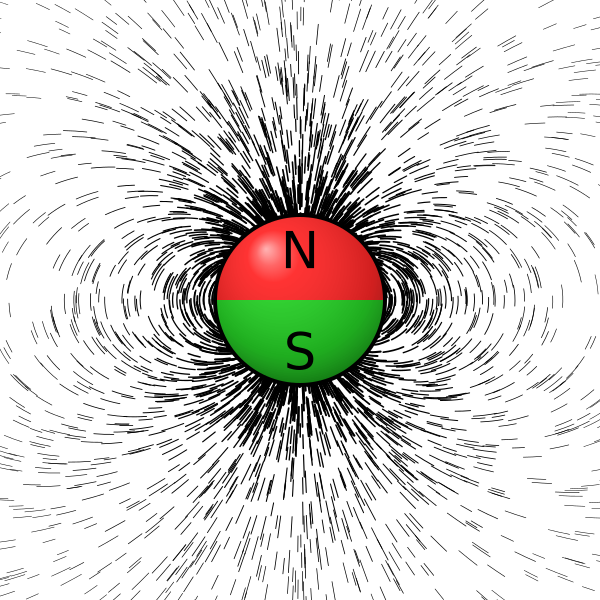
\includegraphics[width=0.4\textwidth]{chapters/chp5_pics/magnet.png}
\caption{\textit{A magnet pulling iron filings is a physical representation of a vector field. Each point around the magnet has a magnitude of force and direction emanating from the magnet}}
\label{fig:magnet}
\end{figure}

\noindent Let's build this idea carefully. Start by imagining a single point $(x_0,y_0)$ in the plane. At this point, we want to attach a vector—perhaps representing wind velocity. This vector will have both an $x$-component and a $y$-component, which we might call $P(x_0,y_0)$ and $Q(x_0,y_0)$ respectively. The vector at this point would then be:
\[
\mathbf{v}_{(x_0,y_0)} = P(x_0,y_0)\mathbf{i} + Q(x_0,y_0)\mathbf{j}
\]

\noindent Now imagine doing this for every point in the plane. As we move to different points $(x,y)$, both components of our vector might change—the wind might blow in different directions and with different speeds at different locations. We're no longer just looking at a single vector, but at a function that assigns a vector to every point. This is the essence of a vector field.

\subsection*{Definition and Basic Properties}

\noindent Formally, a \textbf{vector field} $\mathbf{F}$ in $\mathbb{R}^n$ is a function that assigns to each point $\mathbf{p}$ in its domain a vector $\mathbf{F}(\mathbf{p})$. Just as scalar fields mapped points to numbers, vector fields map points to vectors. In two dimensions, this means associating each point $(x,y)$ with a two-dimensional vector:
\[
\mathbf{F}(x,y) = P(x,y)\mathbf{i} + Q(x,y)\mathbf{j}
\]

\noindent Here, $P(x,y)$ gives the $x$-component of the vector at any point $(x,y)$, while $Q(x,y)$ gives the $y$-component. To understand how this works in practice, let's break down the process of evaluating a vector field at specific points. \\

\noindent Consider a simple vector field $\mathbf{F}(x,y) = x\mathbf{i} + y\mathbf{j}$. Here, $P(x,y) = x$ and $Q(x,y) = y$. To plot vectors in this field:

\begin{center}
\begin{tabular}{|c|c||c|c|c|}
\hline
$x$ & $y$ & Vector Tail at & $P(x,y)$ & $Q(x,y)$ \\
\hline
1 & 1 & (1,1) & 1 & 1 \\
2 & 1 & (2,1) & 2 & 1 \\
1 & 2 & (1,2) & 1 & 2 \\
-1 & 1 & (-1,1) & -1 & 1 \\
\hline
\end{tabular}
\end{center}

\noindent At each point $(x,y)$, we:
\begin{enumerate}
   \item Place the tail of our vector at the point $(x,y)$
   \item Move $P(x,y)$ units in the $\mathbf{i}$ direction
   \item Move $Q(x,y)$ units in the $\mathbf{j}$ direction
\end{enumerate}

\noindent For example, at the point $(2,1)$, we place our vector tail at $(2,1)$, then move 2 units in the $\mathbf{i}$ direction and 1 unit in the $\mathbf{j}$ direction, resulting in a vector pointing to $(4,2)$. \\

\noindent The idea extends naturally to three dimensions. At each point $(x,y,z)$ in space, we now need three components to specify a vector:
\[
\mathbf{F}(x,y,z) = P(x,y,z)\mathbf{i} + Q(x,y,z)\mathbf{j} + R(x,y,z)\mathbf{k}
\]

\noindent For instance, in the three-dimensional vector field $\mathbf{F}(x,y,z) = z\mathbf{i} + x\mathbf{j} + y\mathbf{k}$:

\begin{center}
\begin{tabular}{|c|c|c||c|c|c|}
\hline
$x$ & $y$ & $z$ & $P(x,y,z)$ & $Q(x,y,z)$ & $R(x,y,z)$ \\
\hline
1 & 2 & 3 & 3 & 1 & 2 \\
2 & 1 & 0 & 0 & 2 & 1 \\
-1 & 0 & 2 & 2 & -1 & 0 \\
\hline
\end{tabular}
\end{center}

\noindent At each point $(x,y,z)$, we:
\begin{enumerate}
   \item Place the tail of our vector at the point $(x,y,z)$
   \item Move $P(x,y,z)$ units in the $\mathbf{i}$ direction
   \item Move $Q(x,y,z)$ units in the $\mathbf{j}$ direction
   \item Move $R(x,y,z)$ units in the $\mathbf{k}$ direction
\end{enumerate}

\noindent For example, at the point $(1,2,3)$, the vector starts at $(1,2,3)$ and has components $\langle 3,1,2 \rangle$, meaning it extends 3 units in the $x$-direction, 1 unit in the $y$-direction, and 2 units in the $z$-direction. \\

\noindent The functions $P$, $Q$, and $R$ are called the \textbf{component functions} of the vector field. Each represents the magnitude of the field's projection onto one of the coordinate axes. Just as coordinates tell us where we are in space, these component functions tell us what vector we'll find when we get there. \\

\noindent Just as we studied continuity and differentiability for scalar functions—concepts that told us how ``smoothly" the function varied as we moved around—these ideas extend naturally to vector fields. A vector field is continuous if all its component functions are continuous, meaning the vectors change smoothly as we move from point to point. Similarly, a vector field is differentiable if all its component functions are differentiable, allowing us to analyze rates of change in the field's behavior.


\subsection*{Visualizing Vector Fields}

\noindent After understanding how to evaluate vector fields at individual points, our next step is visualizing them across regions of space. When we plot a vector field, we draw arrows at carefully chosen points to represent the field's behavior. Each arrow has two key properties:
\begin{itemize}
   \item The direction of the arrow shows where the vector field points at that location
   \item The length (or magnitude) of the arrow indicates the vector's strength at that point
\end{itemize}

\noindent Let's develop this systematically. Consider the vector field $\mathbf{F}(x,y) = -y\mathbf{i} + x\mathbf{j}$. To begin visualizing this field, we'll evaluate it at several points using a grid:

\begin{center}
\begin{tabular}{|c|c||c|c|c|}
\hline
$x$ & $y$ & Vector Tail at & $P(x,y) = -y$ & $Q(x,y) = x$ \\
\hline
1 & 1 & (1,1) & -1 & 1 \\
1 & -1 & (1,-1) & 1 & 1 \\
-1 & -1 & (-1,-1) & 1 & -1 \\
-1 & 1 & (-1,1) & -1 & -1 \\
\hline
\end{tabular}
\end{center}

\noindent For each point in our table, we plot a straight arrow by:
\begin{enumerate}
   \item Starting at the tail point $(x,y)$
   \item Drawing a straight line in the direction $\langle P(x,y), Q(x,y) \rangle$
   \item Optionally normalize it by dividing by $\sqrt{P(x,y)^2 + Q(x,y)^2}$
\end{enumerate}

\noindent It's crucial to note that regardless of the vector field, each arrow we draw is always straight—even if the overall pattern suggests rotation or curvature. Each arrow represents the instantaneous direction of the field at a single point. \\

\noindent For example, here's how we would visualize this field:

\begin{center}
\begin{tikzpicture}[scale=1.5]
% Draw axes
\draw[->] (-2,0) -- (2,0) node[right] {$x$};
\draw[->] (0,-2) -- (0,2) node[above] {$y$};

% Draw vectors at diagonal points
\draw[blue,thick,->] (1,1) -- (0,2);
\draw[blue,thick,->] (1,-1) -- (2,0);
\draw[blue,thick,->] (-1,-1) -- (0,-2);
\draw[blue,thick,->] (-1,1) -- (-2,0);

% Label points
\fill (1,1) circle (1pt);
\fill (1,-1) circle (1pt);
\fill (-1,-1) circle (1pt);
\fill (-1,1) circle (1pt);

% Add point labels
\node[above right] at (1,1) {$(1,1)$};
\node[below right] at (1,-1) {$(1,-1)$};
\node[below left] at (-1,-1) {$(-1,-1)$};
\node[above left] at (-1,1) {$(-1,1)$};
\end{tikzpicture}
\end{center}

\noindent Notice how even with just these four points, we can begin to see the rotational pattern emerging in the field. Together the arrows suggest a counterclockwise circulation around the origin. Here's an example of a complete field generated systematically for $\mathbf{F}(x,y) = -y\mathbf{i} + x\mathbf{j}$:

\begin{figure}[H]
\centering
   \begin{tikzpicture}
       \begin{axis}[
           xmin = -4, xmax = 4,
           ymin = -4, ymax = 4,
           zmin = 0, zmax = 1,
           axis equal image,
           xtick distance = 1,
           ytick distance = 1,
           view = {0}{90},
           scale = 1.25,
           title = {\bf Vector Field $F = [-y,x]$},
           height=7cm,
           xlabel = {$x$},
           ylabel = {$y$},
           colormap/viridis,
           colorbar,
           colorbar style = {
               ylabel = {Vector Length}
           }
       ]
           \addplot3[
               point meta = {sqrt(x^2+y^2)},
               quiver = {
                   u = {-y/sqrt(x^2+y^2)},
                   v = {x/sqrt(x^2+y^2)},
                   scale arrows = 0.25,
               },
               quiver/colored = {mapped color},
               -stealth,
               domain = -4:4,
               domain y = -4:4,
           ] {0};
       \end{axis}
   \end{tikzpicture}
\caption{\textit{The circular pattern emerges from the collective behavior of many straight arrows, each showing the instantaneous direction at its starting point. This is analogous to how the tangent line approximates a curve at a single point—each vector arrow shows the field's direction at just one point in space.}}
\end{figure}


\noindent When we plot many more points, patterns emerge in the vector field. These patterns help us identify important features:

\begin{itemize}
   \item \textbf{Sources:} Points where vectors emanate outward, like water springing from a fountain. For example, in the field $\mathbf{F}(x,y) = x\mathbf{i} + y\mathbf{j}$, the origin is a source:
   
   \begin{figure}[H]
   \centering
   \begin{tikzpicture}
   \begin{axis}[
       xmin = -4, xmax = 4,
       ymin = -4, ymax = 4,
       zmin = 0, zmax = 1,
       axis equal image,
       xtick distance = 1,
       ytick distance = 1,
       view = {0}{90},
       scale = 1.25,
       title = {\bf Source Field: $F = [x,y]$},
       height=7cm,
       xlabel = {$x$},
       ylabel = {$y$},
       colormap/viridis,
       colorbar,
       colorbar style = {
           ylabel = {Vector Length}
       }
   ]
       \addplot3[
           point meta = {sqrt(x^2+y^2)},
           quiver = {
               u = {x/sqrt(x^2+y^2)},
               v = {y/sqrt(x^2+y^2)},
               scale arrows = 0.25,
           },
           quiver/colored = {mapped color},
           -stealth,
           domain = -4:4,
           domain y = -4:4,
       ] {0};
   \end{axis}
   \end{tikzpicture}
   \end{figure}

   \item \textbf{Sinks:} Points where vectors converge inward, like water draining from a bathtub. The field $\mathbf{F}(x,y) = -x\mathbf{i} - y\mathbf{j}$ has a sink at the origin:
   
   \begin{figure}[H]
   \centering
   \begin{tikzpicture}
   \begin{axis}[
       xmin = -4, xmax = 4,
       ymin = -4, ymax = 4,
       zmin = 0, zmax = 1,
       axis equal image,
       xtick distance = 1,
       ytick distance = 1,
       view = {0}{90},
       scale = 1.25,
       title = {\bf Sink Field: $F = [-x,-y]$},
       height=7cm,
       xlabel = {$x$},
       ylabel = {$y$},
       colormap/viridis,
       colorbar,
       colorbar style = {
           ylabel = {Vector Length}
       }
   ]
       \addplot3[
           point meta = {sqrt(x^2+y^2)},
           quiver = {
               u = {-x/sqrt(x^2+y^2)},
               v = {-y/sqrt(x^2+y^2)},
               scale arrows = 0.25,
           },
           quiver/colored = {mapped color},
           -stealth,
           domain = -4:4,
           domain y = -4:4,
       ] {0};
   \end{axis}
   \end{tikzpicture}
   \end{figure}

   \item \textbf{Circulation:} Regions where vectors suggest rotational motion, like our example field $\mathbf{F}(x,y) = -y\mathbf{i} + x\mathbf{j}$. Remember though—each individual arrow is still straight!
   
   \begin{figure}[H]
   \centering
   \begin{tikzpicture}
   \begin{axis}[
       xmin = -4, xmax = 4,
       ymin = -4, ymax = 4,
       zmin = 0, zmax = 1,
       axis equal image,
       xtick distance = 1,
       ytick distance = 1,
       view = {0}{90},
       scale = 1.25,
       title = {\bf Circulation Field: $F = [-y,x]$},
       height=7cm,
       xlabel = {$x$},
       ylabel = {$y$},
       colormap/viridis,
       colorbar,
       colorbar style = {
           ylabel = {Vector Length}
       }
   ]
       \addplot3[
           point meta = {sqrt(x^2+y^2)},
           quiver = {
               u = {-y/sqrt(x^2+y^2)},
               v = {x/sqrt(x^2+y^2)},
               scale arrows = 0.25,
           },
           quiver/colored = {mapped color},
           -stealth,
           domain = -4:4,
           domain y = -4:4,
       ] {0};
   \end{axis}
   \end{tikzpicture}
   \end{figure}

   \item \textbf{Saddle Points:} Points exhibiting both attractive and repulsive behavior, like the origin in $\mathbf{F}(x,y) = x\mathbf{i} - y\mathbf{j}$:
   
   \begin{figure}[H]
   \centering
   \begin{tikzpicture}
   \begin{axis}[
       xmin = -4, xmax = 4,
       ymin = -4, ymax = 4,
       zmin = 0, zmax = 1,
       axis equal image,
       xtick distance = 1,
       ytick distance = 1,
       view = {0}{90},
       scale = 1.25,
       title = {\bf Saddle Field: $F = [x,-y]$},
       height=7cm,
       xlabel = {$x$},
       ylabel = {$y$},
       colormap/viridis,
       colorbar,
       colorbar style = {
           ylabel = {Vector Length}
       }
   ]
       \addplot3[
           point meta = {sqrt(x^2+y^2)},
           quiver = {
               u = {x/sqrt(x^2+y^2)},
               v = {-y/sqrt(x^2+y^2)},
               scale arrows = 0.25,
           },
           quiver/colored = {mapped color},
           -stealth,
           domain = -4:4,
           domain y = -4:4,
       ] {0};
   \end{axis}
   \end{tikzpicture}
   \end{figure}
\end{itemize}

\noindent Notice how the colors in these plots indicate the magnitude of the vectors at each point. Brighter colors represent stronger vectors, while darker colors show regions where the field is weaker. The origin (0,0) plays a special role in each of these fields, serving as the central point around which the field's behavior is organized.\\

\noindent Below is a Python script that can be used to visualize vector fields since it requires a lot of computation. Use it to aid you in your sketches for the examples to come.


\vspace{1.3em} \index{Python}


\begin{lstlisting}[language=Python]
import numpy as np
import matplotlib.pyplot as plt

# Define the functions P(x, y) and Q(x, y)
def P(x, y):
   return -y  # Example: -y

def Q(x, y):
   return x  # Example: x

# Create the grid
x, y = np.meshgrid(np.linspace(-10, 10, 25), np.linspace(-10, 10, 25))

# Compute the vector components
u = P(x, y)
v = Q(x, y)

# Normalize vectors to minimize arrow crossings
magnitude = np.sqrt(u**2 + v**2)
u = u / magnitude
v = v / magnitude

# Plot the vector field
plt.quiver(x, y, u, v, angles='xy', scale_units='xy', scale=1, color='blue', width=0.0025)
plt.xlim(-10, 10)
plt.ylim(-10, 10)
plt.xlabel('x')
plt.ylabel('y')
plt.title('2D Vector Field')
plt.grid()
plt.show()
\end{lstlisting}

\vspace{1.3em}

\subsubsection*{Understanding Vector Field Normalization}

\noindent When visualizing vector fields, we often face a choice between showing the true magnitudes of our vectors and normalizing them to unit length. This decision fundamentally impacts what information we can glean from our visualization. Just as we might choose different coordinate systems based on the symmetries of a problem, we must thoughtfully consider when to normalize our vector fields. \\

\noindent To normalize a vector field $\mathbf{F}(x,y) = P(x,y)\mathbf{i} + Q(x,y)\mathbf{j}$, we divide by its magnitude at each point:
\[
\mathbf{F}_{\text{norm}}(x,y) = \frac{P(x,y)}{\sqrt{P(x,y)^2 + Q(x,y)^2}}\mathbf{i} + \frac{Q(x,y)}{\sqrt{P(x,y)^2 + Q(x,y)^2}}\mathbf{j}
\]

\noindent This transformation preserves the direction of each vector while scaling them all to unit length. Consider the field $\mathbf{F}(x,y) = (x^2-y^2)\mathbf{i} + (2xy)\mathbf{j}$. In its normalized form, the quadratic growth in magnitude disappears, revealing purely directional information about the field. Alternatively, without normalization the magnitudes would cause eventual overlapping which would make the visualization unwieldy.\\

\noindent The decision to normalize a vector field should be guided by our analytical goals. Normalization is particularly valuable when:

\begin{enumerate}
   \item \textbf{Directional Analysis is Primary:} When we need to understand the flow patterns or trajectories in our field, normalization helps by eliminating the potentially distracting variations in magnitude. This is especially useful in studying fluid flow patterns, magnetic field lines, or gravitational field directions.
   
   \item \textbf{Visual Clarity is Crucial:} In fields with large magnitude variations, like our quadratic example, smaller vectors can become nearly invisible compared to larger ones. Normalization ensures each vector contributes equally to our visual understanding.
   
   \item \textbf{Pattern Recognition is Key:} Normalized fields often reveal symmetries, circulation patterns, and topological features that might be obscured by magnitude variations. For instance, the rotational nature of our quadratic field becomes much clearer after normalization.
\end{enumerate}

\noindent However, normalization isn't always appropriate. We should maintain the original magnitudes when:

\begin{enumerate}
   \item \textbf{Magnitude Information is Essential:} In many physical applications, vector magnitude carries crucial information. A velocity field in fluid dynamics, for instance, needs its magnitude preserved to show where flow is fastest or slowest.
   
   \item \textbf{Physical Accuracy Matters:} For quantitative analysis or physical simulations, preserving true vector magnitudes is often crucial. For example, when studying force fields, the strength of the force is just as important as its direction.
\end{enumerate}

\noindent Just as a topographic map might show both elevation contours and gradient directions, we can often benefit from examining both normalized and unnormalized versions of a vector field. The normalized field reveals pure directional patterns, while the unnormalized field preserves magnitude information. Together, they provide a complete picture of the field's behavior.

\exampleline
\begin{example}
Classify and visualize the following vector fields:
\begin{enumerate}
   \item $\mathbf{F}(x,y) = \frac{x}{\sqrt{x^2+y^2}}\mathbf{i} + \frac{y}{\sqrt{x^2+y^2}}\mathbf{j}$
   \item $\mathbf{F}(x,y) = \frac{x^2-y^2}{\sqrt{(x^2-y^2)^2 + (2xy)^2}}\mathbf{i} + \frac{2xy}{\sqrt{(x^2-y^2)^2 + (2xy)^2}}\mathbf{j}$
\end{enumerate}

\begin{solution}
Let's analyze each field systematically:

\begin{enumerate}
   \item For $\mathbf{F}(x,y) = \frac{x}{\sqrt{x^2+y^2}}\mathbf{i} + \frac{y}{\sqrt{x^2+y^2}}\mathbf{j}$:
   
   Let's first understand what this field does:
   \begin{itemize}
       \item The denominator $\sqrt{x^2+y^2}$ represents the distance from the origin to point $(x,y)$
       \item At each point $(x,y)$, dividing by this distance normalizes our vector to unit length
       \item The field gives us a way to point outward from the origin in every direction
   \end{itemize}
   
   Let's evaluate at eight points around the origin:
   \begin{center}
   \begin{tabular}{|c|c||c|c|c|}
   \hline
   $(x,y)$ & $\sqrt{x^2+y^2}$ & $P(x,y)$ & $Q(x,y)$ & Direction \\
   \hline
   $(1,0)$ & 1 & 1 & 0 & Right \\
   $(1,1)$ & $\sqrt{2}$ & $\frac{1}{\sqrt{2}}$ & $\frac{1}{\sqrt{2}}$ & NE diagonal \\
   $(0,1)$ & 1 & 0 & 1 & Up \\
   $(-1,1)$ & $\sqrt{2}$ & $-\frac{1}{\sqrt{2}}$ & $\frac{1}{\sqrt{2}}$ & NW diagonal \\
   $(-1,0)$ & 1 & -1 & 0 & Left \\
   $(-1,-1)$ & $\sqrt{2}$ & $-\frac{1}{\sqrt{2}}$ & $-\frac{1}{\sqrt{2}}$ & SW diagonal \\
   $(0,-1)$ & 1 & 0 & -1 & Down \\
   $(1,-1)$ & $\sqrt{2}$ & $\frac{1}{\sqrt{2}}$ & $-\frac{1}{\sqrt{2}}$ & SE diagonal \\
   \hline
   \end{tabular}
   \end{center}
   
   Here's a rough sketch showing these eight unit vectors:
   
   \begin{center}
   \begin{tikzpicture}[scale=1.5]
   % Draw axes
   \draw[->] (-2,0) -- (2,0) node[right] {$x$};
   \draw[->] (0,-2) -- (0,2) node[above] {$y$};
   
   % Draw the eight unit vectors
   \draw[blue,thick,->] (1,0) -- (2,0);
   \draw[blue,thick,->] (1,1) -- (1.7,1.7);
   \draw[blue,thick,->] (0,1) -- (0,2);
   \draw[blue,thick,->] (-1,1) -- (-1.7,1.7);
   \draw[blue,thick,->] (-1,0) -- (-2,0);
   \draw[blue,thick,->] (-1,-1) -- (-1.7,-1.7);
   \draw[blue,thick,->] (0,-1) -- (0,-2);
   \draw[blue,thick,->] (1,-1) -- (1.7,-1.7);
   
   % Label points
   \fill (1,0) circle (1pt);
   \fill (1,1) circle (1pt);
   \fill (0,1) circle (1pt);
   \fill (-1,1) circle (1pt);
   \fill (-1,0) circle (1pt);
   \fill (-1,-1) circle (1pt);
   \fill (0,-1) circle (1pt);
   \fill (1,-1) circle (1pt);
   
   % Label origin
   \node at (0,0) {$\bullet$};
   \node[below right] at (0,0) {$O$};
   
   % Labels for some key points
   \node[right] at (1,.3) {\tiny$(1,0)$};
   \node[above right] at (1,0.8) {\tiny$(1,1)$};
   \node[left] at (-1,.3) {\tiny$(-1,0)$};
   \end{tikzpicture}
   \end{center}
   
   Several important properties emerge from our analysis:
   \begin{itemize}
       \item Every vector has length 1 (they're normalized)
       \item Each vector points directly away from the origin
       \item The field is undefined at the origin (division by zero)
       \item The pattern has radial symmetry about the origin
   \end{itemize}

   The computer-generated vector field looks like this:
   
\begin{figure}[H]
\centering
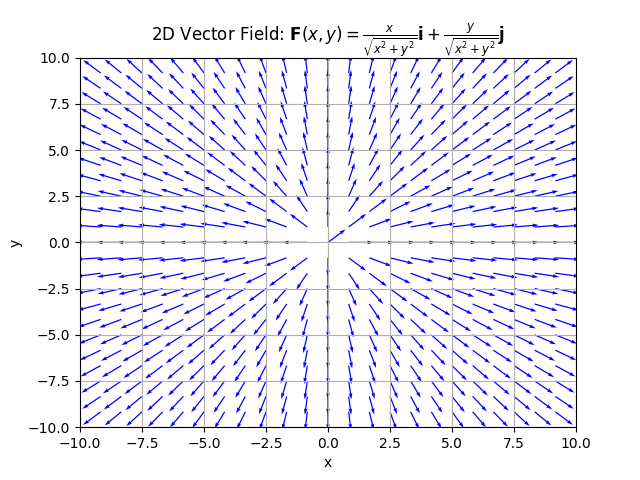
\includegraphics[width=0.8\textwidth]{chapters/chp5_pics/5.1.1-1.png}
\label{fig:5.1.1-1}
\end{figure}
   
   This is a \textbf{source field} with unit vectors. All vectors point outward from the origin with equal magnitude. It's similar to the electric field of a positive point charge or the field lines emerging from a magnetic monopole (if one existed).
   
\item For $\mathbf{F}(x,y) = \frac{x^2-y^2}{\sqrt{(x^2-y^2)^2 + (2xy)^2}}\mathbf{i} + \frac{2xy}{\sqrt{(x^2-y^2)^2 + (2xy)^2}}\mathbf{j}$

This normalized version of our previous field will help us understand its pure directional behavior. At each point, we're taking the same direction but scaling it to have unit length. Let's understand how we got here:

\begin{itemize}
   \item The original field was $\mathbf{F}(x,y) = (x^2-y^2)\mathbf{i} + (2xy)\mathbf{j}$
   \item Its magnitude at any point is $\sqrt{(x^2-y^2)^2 + (2xy)^2}$
   \item Dividing by this magnitude normalizes each vector to length 1
\end{itemize}

Let's evaluate at carefully chosen points. Since we're normalizing, what matters most is the ratio between components rather than their absolute values:

\begin{center}
\begin{tabular}{|c|c||c|c|c|}
\hline
$(x,y)$ & $\sqrt{(x^2-y^2)^2 + (2xy)^2}$ & $P(x,y)$ & $Q(x,y)$ & Direction \\
\hline
$(1,0)$ & 1 & 1 & 0 & Right \\
$(1,1)$ & 2 & 0 & 1 & Up \\
$(0,1)$ & 1 & -1 & 0 & Left \\
$(-1,1)$ & 2 & 0 & -1 & Down \\
$(-1,0)$ & 1 & 1 & 0 & Right \\
$(-1,-1)$ & 2 & 0 & 1 & Up \\
$(0,-1)$ & 1 & -1 & 0 & Left \\
$(1,-1)$ & 2 & 0 & -1 & Down \\
\hline
\end{tabular}
\end{center}

Let's sketch these unit vectors, being careful to show points at different distances from the origin:

\begin{center}
\begin{tikzpicture}[scale=2]
% Draw axes
\draw[->] (-2,0) -- (2,0) node[right] {$x$};
\draw[->] (0,-2) -- (0,2) node[above] {$y$};

% Draw unit vectors (all length 1)
\draw[blue,thick,->] (1,1) -- (1,2);
\draw[blue,thick,->] (1,-1) -- (1,-2);
\draw[blue,thick,->] (1,0) -- (2,0);
\draw[blue,thick,->] (0,1) -- (-1,1);
\draw[blue,thick,->] (2,1) -- (2.6,1.8);
\draw[blue,thick,->] (1.414,1.414) -- (1.414,2.414);  % √2 points
\draw[blue,thick,->] (2,0) -- (3,0);
\draw[blue,thick,->] (0,2) -- (-1,2);
\draw[blue,thick,->] (2,-1) -- (2.6,-1.8);
\draw[blue,thick,->] (0.707,0.707) -- (0.707,1.707);  % 1/√2 points

% Label points
\fill (1,1) circle (1pt) node[above right] {\tiny$(1,1)$};
\fill (1,0) circle (1pt) node[below] {\tiny$(1,0)$};
\fill (2,1) circle (1pt) node[right] {\tiny$(2,1)$};
\fill (1.414,1.414) circle (1pt) node[above right] {\tiny$(\sqrt{2},\sqrt{2})$};
\fill (2,0) circle (1pt) node[below] {\tiny$(2,0)$};
\fill (0.707,0.707) circle (1pt) node[above left] {\tiny$(\frac{1}{\sqrt{2}},\frac{1}{\sqrt{2}})$};

% Label origin
\node at (0,0) {$\bullet$};
\node[below right] at (0,0) {$O$};
\end{tikzpicture}
\end{center}

These additional points help reveal even more patterns in the field:
\begin{itemize}
   \item The same directional pattern appears at all distances from the origin - notice how points like $(1,1)$ and $(\frac{1}{\sqrt{2}},\frac{1}{\sqrt{2}})$ show identical behavior despite being at different distances
   \item Along rays from the origin (like the points $(1,0)$ and $(2,0)$), vectors point in exactly the same direction
   \item The transition between vertical and horizontal flow is smooth and consistent at all distances
   \item Each point's vector direction depends only on the ratio of $y$ to $x$, not on their absolute values
\end{itemize}

The computer-generated vector field looks like this:

\begin{figure}[H]
\centering
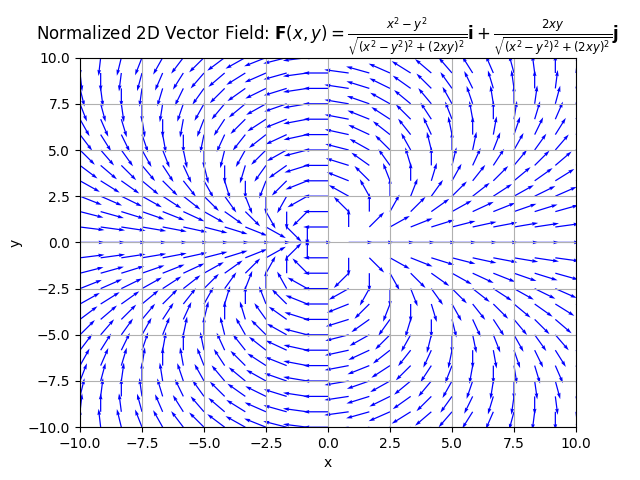
\includegraphics[width=0.8\textwidth]{chapters/chp5_pics/5.1.1-2.png}
\label{fig:5.1.1-2}
\end{figure}

This normalized version of the field reveals its pure directional behavior. Now we can see clearly how the field creates a twisted circulation pattern, with vectors smoothly transitioning between vertical flow along diagonals and horizontal flow near the axes. This type of normalization is often useful in physics when we care more about the direction of a force or flow than its magnitude, such as in studying the directional patterns of complex fluid flows.
\end{enumerate}
\end{solution}
\end{example}
\exampleline

\subsection*{Conservative Vector Fields} \index{Conservative Fields}

\noindent When studying vector fields, one of the most fundamental questions we can ask is whether the field represents a quantity that depends only on position, or one that depends on how we got to that position. This distinction leads us to the crucial concept of conservative vector fields. \\

\noindent A vector field $\mathbf{F}$ is called \textbf{conservative} if there exists a scalar function $f$, called a \textbf{potential function}, such that:
\[
\mathbf{F} = \nabla f
\]

\noindent In two dimensions, this means:
\[
P(x,y) = \frac{\partial f}{\partial x} \quad \text{and} \quad Q(x,y) = \frac{\partial f}{\partial y}
\]

\noindent And in three dimensions:
\[
P(x,y,z) = \frac{\partial f}{\partial x}, \quad Q(x,y,z) = \frac{\partial f}{\partial y}, \quad \text{and} \quad R(x,y,z) = \frac{\partial f}{\partial z}
\]

\noindent The term ``conservative" comes from the fact that these fields conserve energy—there's no loss or gain of energy when moving along a closed path. This leads to several critical properties:

\begin{itemize}
   \item The work done by a conservative field along any path between two points depends only on the endpoints, not on the path taken
   \item The curl of a conservative field is zero (a fact we'll explore in detail later)
   \item Line integrals of conservative fields around closed paths are always zero
\end{itemize}

\noindent When a field is not conservative, we call it \textbf{non-conservative} or \textbf{rotational}. Understanding whether a field is conservative or non-conservative has profound implications in physics and engineering:

\begin{itemize}
   \item \textbf{Conservative Fields:}
       \begin{itemize}
           \item Gravitational fields
           \item Electrostatic fields
           \item Pressure gradients in static fluids
       \end{itemize}
       
   \item \textbf{Non-Conservative Fields:} \index{Non-Conservative Fields}
       \begin{itemize}
           \item Magnetic fields
           \item Friction forces
           \item Velocity fields in rotating fluids
       \end{itemize}
\end{itemize}

\subsection*{Testing for Conservative Fields}

\noindent Not all vector fields are conservative. The key test involves examining the field's partial derivatives. In two dimensions, if $\mathbf{F}(x,y) = P\mathbf{i} + Q\mathbf{j}$ is defined on a simply connected domain, then $\mathbf{F}$ is conservative if and only if:
\[
\frac{\partial P}{\partial y} = \frac{\partial Q}{\partial x}
\]

\noindent This condition arises from the equality of mixed partial derivatives of the potential function:
\[
\frac{\partial^2 f}{\partial y\partial x} = \frac{\partial^2 f}{\partial x\partial y}
\]

\noindent In three dimensions, a vector field $\mathbf{F}(x,y,z) = P\mathbf{i} + Q\mathbf{j} + R\mathbf{k}$ defined on a simply connected domain is conservative if and only if:
\[
\frac{\partial P}{\partial y} = \frac{\partial Q}{\partial x}, \quad
\frac{\partial P}{\partial z} = \frac{\partial R}{\partial x}, \quad
\frac{\partial Q}{\partial z} = \frac{\partial R}{\partial y}
\]

\noindent The significance of conservative fields extends far beyond these mathematical conditions. Consider these practical implications:

\begin{enumerate}
   \item \textbf{Energy Conservation:} In conservative systems, energy is perfectly conserved. A ball rolling in a gravitational field (ignoring friction) will reach the same height regardless of the path it takes.
   
   \item \textbf{Path Independence:} The work done by conservative forces depends only on start and end positions. This means we can choose the most convenient path for our calculations.
   
   \item \textbf{Potential Functions:} Conservative fields allow us to define potential energy functions, greatly simplifying many physical calculations. Instead of computing complicated path integrals, we can just evaluate the potential function at endpoints.
   
   \item \textbf{Equilibrium Analysis:} The existence of a potential function helps identify stable and unstable equilibrium points in physical systems.
\end{enumerate}

\noindent In contrast, non-conservative fields exhibit fundamentally different behavior:
\begin{enumerate}
   \item They can do different amounts of work along different paths
   \item They can add or remove energy from a system
   \item They often represent dissipative forces or fields that depend on velocity
   \item They cannot be derived from a potential function
\end{enumerate}

\noindent This distinction between conservative and non-conservative fields is crucial in physics and engineering. For instance, when designing energy systems, knowing whether forces are conservative helps predict whether energy will be conserved or dissipated. In fluid dynamics, identifying non-conservative velocity fields helps understand where energy losses occur. Even in economics, conservative fields can model ideal market behaviors, while non-conservative fields might better represent real markets with friction and inefficiencies.


\exampleline
\begin{example}
Let's see what kind of fields Example 5.1.1 had (with the second example being changed to non-normalized for ease of differentiation). Please classify them as either Conservative or Non-Conservative:

\begin{enumerate}
   \item The normalized radial field $\mathbf{F}(x,y) = \frac{x}{\sqrt{x^2+y^2}}\mathbf{i} + \frac{y}{\sqrt{x^2+y^2}}\mathbf{j}$
   
   \item The quadratic field $\mathbf{F}(x,y) = (x^2-y^2)\mathbf{i} + (2xy)\mathbf{j}$
\end{enumerate}

Determine whether each field is conservative by testing the condition $\frac{\partial P}{\partial y} = \frac{\partial Q}{\partial x}$.

\begin{solution}
Let's analyze each field systematically:

\begin{enumerate}
   \item For the normalized radial field, let:
   \[
   P(x,y) = \frac{x}{\sqrt{x^2+y^2}} \quad \text{and} \quad Q(x,y) = \frac{y}{\sqrt{x^2+y^2}}
   \]
   
   First, compute $\frac{\partial P}{\partial y}$ using the quotient rule:
   \begin{align*}
   \frac{\partial P}{\partial y} &= \frac{\partial}{\partial y}\left(\frac{x}{\sqrt{x^2+y^2}}\right) \\
   &= x \cdot \frac{\partial}{\partial y}\left(\frac{1}{\sqrt{x^2+y^2}}\right) \\
   &= x \cdot \left(-\frac{1}{2}(x^2+y^2)^{-3/2} \cdot 2y\right) \\
   &= -\frac{xy}{(x^2+y^2)^{3/2}}
   \end{align*}
   
   Next, compute $\frac{\partial Q}{\partial x}$:
   \begin{align*}
   \frac{\partial Q}{\partial x} &= \frac{\partial}{\partial x}\left(\frac{y}{\sqrt{x^2+y^2}}\right) \\
   &= y \cdot \frac{\partial}{\partial x}\left(\frac{1}{\sqrt{x^2+y^2}}\right) \\
   &= y \cdot \left(-\frac{1}{2}(x^2+y^2)^{-3/2} \cdot 2x\right) \\
   &= -\frac{xy}{(x^2+y^2)^{3/2}}
   \end{align*}
   
   Since $\frac{\partial P}{\partial y} = \frac{\partial Q}{\partial x}$, this field is conservative. Indeed, we can find its potential function: $f(x,y) = \sqrt{x^2+y^2}$. This explains why this normalized field points radially outward—it represents the direction of steepest increase of the distance function from the origin.
   
   \item For the quadratic field, let:
   \[
   P(x,y) = x^2-y^2 \quad \text{and} \quad Q(x,y) = 2xy
   \]
   
   Computing the partial derivatives:
   \begin{align*}
   \frac{\partial P}{\partial y} &= \frac{\partial}{\partial y}(x^2-y^2) = -2y \\
   \frac{\partial Q}{\partial x} &= \frac{\partial}{\partial x}(2xy) = 2y
   \end{align*}
   
   Since $\frac{\partial P}{\partial y} = -2y \neq 2y = \frac{\partial Q}{\partial x}$, this field is non-conservative. This aligns with our earlier observation of its rotational behavior—the field exhibits a circulation pattern that cannot be derived from any potential function. If we were to compute the work done by this field along different paths between the same points, we would get different results.
\end{enumerate}
\end{solution}
\end{example}
\exampleline











\newpage

\lecture{Line Integrals} \index{Line Integrals}

\noindent After our exploration of vector fields, we now turn to one of the most fundamental operations we can perform on them: integration along curves. Just as we previously extended single-variable integration to multiple dimensions through multiple integrals, we'll now develop the tools to integrate both scalar functions and vector fields along paths in space. This concept will prove crucial in physics, engineering, and advanced mathematics.

\subsection*{Line Integrals of Scalar Functions}

\noindent Before diving into vector fields, let's start with a simpler scenario: integrating a scalar function along a curve. Imagine walking along a curved path on a hilly terrain. At each point, there's an elevation—a scalar value associated with your position. If we wanted to calculate the ``total elevation" experienced along our path, we'd need a line integral. \\

\noindent Recall from Chapter 2 Lecture 4 that we developed the concept of arc length for a parametric curve. Given a curve $C$ parameterized by $\mathbf{r}(t) = x(t)\mathbf{i} + y(t)\mathbf{j}$ for $a \leq t \leq b$, we found its length using:
\[
L = \int_a^b \sqrt{\left(\frac{dx}{dt}\right)^2 + \left(\frac{dy}{dt}\right)^2}\,dt = \int_a^b \left\|\frac{d\mathbf{r}}{dt}\right\|\,dt
\]

\noindent Now imagine that at each point along this curve, we're not just measuring distance but also evaluating some scalar function $f(x,y)$. We can think of this as ``weighting" each infinitesimal piece of arc length by the value of $f$ at that point. This leads naturally to the line integral:
\[
\int_C f(x,y)\,ds = \int_a^b f(x(t),y(t))\sqrt{\left(\frac{dx}{dt}\right)^2 + \left(\frac{dy}{dt}\right)^2}\,dt
\]
\noindent We note that this will yield us an area, because we are multiplying the arc length by a height function. Let's break down the components of this integral:
\begin{itemize}
    \item $f(x(t),y(t))$ evaluates our scalar function at each point along $C$
    \item $\sqrt{\left(\frac{dx}{dt}\right)^2 + \left(\frac{dy}{dt}\right)^2}\,dt$ gives us the infinitesimal arc length $ds$
    \item Their product $f(x(t),y(t))\,ds$ represents the contribution of each tiny piece of the curve
\end{itemize}

\noindent This geometric interpretation helps us understand several key properties:

\begin{enumerate}
    \item \textbf{Reparametrization Invariance:} The value of the line integral doesn't depend on how we parameterize $C$. Different parameters will adjust both $f(x(t),y(t))$ and $\frac{d\mathbf{r}}{dt}$, but their product remains constant.
    
    \item \textbf{Direction Independence:} For scalar line integrals, the direction we traverse $C$ doesn't matter. This is because $ds$ is always positive, measuring pure distance rather than directed movement.

\begin{figure}[H]
\centering
\begin{tikzpicture}
\begin{axis}[
    view={60}{20},  % Adjusted view angle for better visibility underneath
    axis lines=middle,
    xlabel={$x$},
    ylabel={$y$},
    zlabel={$z$},
    grid=none,
    ticks=none,
    width=12cm,
    height=12cm,
    xmin=-3, xmax=3,
    ymin=-3, ymax=3,
    zmin=0, zmax=4,  % Lifted up the z-range
    samples=40,
    domain=-3:3,
    y domain=-3:3,
    colormap/cool,
    clip=false
]

% Draw the undulating surface
\addplot3[
    surf,
    faceted color=blue!10,  % Made surface color lighter
    opacity=0.4,  % More transparent
    shader=flat,
] {2 + 0.3*sin(deg(2*x))*cos(deg(2*y))};  % Centered and lifted surface

% Fill the area under the curve with semi-transparent sheets
\pgfplotsinvokeforeach{0,0.02,...,1}{
    % Create fill between curve and xy-plane
    \addplot3[
        fill=cyan!20,  % Light cyan fill
        opacity=0.1,  % Very transparent for layered effect
        draw=none
    ] coordinates {
        ({1.5*cos(360*#1)}, {1.5*sin(360*#1)}, 0)
        ({1.5*cos(360*#1)}, {1.5*sin(360*#1)}, {2 + 0.3*sin(deg(3*cos(360*#1)))*cos(deg(3*sin(360*#1)))})
        ({1.5*cos(360*#1 + 1)}, {1.5*sin(360*#1 + 1)}, {2 + 0.3*sin(deg(3*cos(360*#1 + 1)))*cos(deg(3*sin(360*#1 + 1)))})
        ({1.5*cos(360*#1 + 1)}, {1.5*sin(360*#1 + 1)}, 0)
    };
}

% Draw vertical lines for the "curtain" effect
\pgfplotsinvokeforeach{0,0.1,...,1}{
    \addplot3[cyan!30, thin] coordinates {
        ({1.5*cos(360*#1)}, {1.5*sin(360*#1)}, 0)
        ({1.5*cos(360*#1)}, {1.5*sin(360*#1)}, {2 + 0.3*sin(deg(3*cos(360*#1)))*cos(deg(3*sin(360*#1)))})
    };
}

% Draw the curve on the surface
\addplot3[
    red!80,  % Slightly dimmer red
    thick,
    samples=50,
    domain=0:360,
] ({1.5*cos(x)}, {1.5*sin(x)}, {2 + 0.3*sin(deg(3*cos(x)))*cos(deg(3*sin(x)))});

% Draw the projected curve on xy-plane
\addplot3[
    magenta!70,  % Dimmer magenta
    thick,
    dashed,
    samples=50,
    domain=0:360,
] ({1.5*cos(x)}, {1.5*sin(x)}, 0);

% Add labels
\node[anchor=north] at (axis cs:2,0,0) {$C$};
\node[anchor=south] at (axis cs:0,2,3) {$z=f(x,y)$};
\node[anchor=west] at (axis cs:0,-4,1) {$\displaystyle\int_C f(x,y)\,ds$};

% Add a small ds element indicator
\draw[magenta,->,thick] (axis cs:0,1.5,0) -- (axis cs:0.2,1.5,0) node[midway,above] {$ds$};

\end{axis}
\end{tikzpicture}
\caption{\textit{Geometric interpretation of a scalar line integral $\int_C f(x,y)\,ds$. The curve $C$ (shown in red) lies on the surface $z=f(x,y)$, while its projection onto the $xy$-plane is shown as a dashed magenta curve. The shaded ``curtain" between these curves represents the accumulation of the function values along the path, with each vertical height $f(x,y)$ being weighted by the infinitesimal arc length $ds$.}}
\label{fig:scalar_line_integral}
\end{figure}
    
    \item \textbf{Physical Meaning:} The integral accumulates the product of the scalar field and distance traveled, giving us meaningful physical quantities:
    \begin{itemize}
        \item Mass = $\int_C \rho(x,y)\,ds$ where $\rho$ is linear density
        \item Cost = $\int_C c(x,y)\,ds$ where $c$ is cost per unit length
        \item Average value of $f$ along $C$ = $\frac{1}{L}\int_C f(x,y)\,ds$ where $L$ is the arc length
    \end{itemize}
\end{enumerate}

\noindent The computation process follows these steps:
\begin{enumerate}
    \item Express the curve $C$ parametrically: $\mathbf{r}(t) = x(t)\mathbf{i} + y(t)\mathbf{j}$
    \item Calculate $\frac{dx}{dt}$ and $\frac{dy}{dt}$
    \item Compose $f$ with the parametrization: $f(x(t),y(t))$
    \item Form the integrand: $f(x(t),y(t))\sqrt{\left(\frac{dx}{dt}\right)^2 + \left(\frac{dy}{dt}\right)^2}$
    \item Integrate with respect to $t$ from $a$ to $b$
\end{enumerate}


\noindent You may encounter an alternative notation for line integrals, particularly in complex analysis and physics: the contour integral. Written as $\oint_C f(x,y)\,ds$, this notation emphasizes that we're integrating along a specific path or contour in the plane. The circle in the integral symbol traditionally suggests a closed path—one that returns to its starting point. While we'll primarily use $\int_C$ notation in our development of vector calculus, recognizing the contour notation is crucial as it appears frequently in applications, especially when dealing with conservative fields and path independence. \\

\exampleline
\begin{example}
Evaluate the line integral $\int_C f(x,y)\,ds$ where $f(x,y) = y-2x$ along:
\begin{enumerate}
    \item The curve $C_1$ given by $\mathbf{r}(t) = (2t)\mathbf{i} + (3t)\mathbf{j}$, $0 \leq t \leq 1$
    \item The curve $C_2$ given by $\mathbf{r}(t) = (\cos t)\mathbf{i} + (2\sin t)\mathbf{j}$, $0 \leq t \leq 2\pi$
\end{enumerate}
\begin{solution}
Let's evaluate each integral systematically:
\begin{enumerate}
    \item For curve $C_1$:
    
    First, we need:
    \begin{itemize}
        \item $\frac{dx}{dt} = 2$, $\frac{dy}{dt} = 3$
        \item $f(x(t),y(t)) = 3t-4t = -t$ 
        \item $ds = \sqrt{(\frac{dx}{dt})^2 + (\frac{dy}{dt})^2}\,dt = \sqrt{4+9}\,dt = \sqrt{13}\,dt$
    \end{itemize}
    
    Therefore:
    \begin{align*}
        \int_C f(x,y)\,ds &= \int_0^1 (-t)(\sqrt{13})\,dt \\
        &= -\sqrt{13}\int_0^1 t\,dt \\
        &= -\sqrt{13}[\frac{t^2}{2}]_0^1 \\
        &= -\frac{\sqrt{13}}{2}
    \end{align*}
    
    \item For curve $C_2$:
    
    We need:
    \begin{itemize}
        \item $\frac{dx}{dt} = -\sin t$, $\frac{dy}{dt} = 2\cos t$
        \item $f(x(t),y(t)) = 2\sin t - 2\cos t$
        \item $ds = \sqrt{(\frac{dx}{dt})^2 + (\frac{dy}{dt})^2}\,dt = \sqrt{\sin^2 t + 4\cos^2 t}\,dt$
    \end{itemize}
    
    Therefore:
    \begin{align*}
        \oint_C f(x,y)\,ds &= \int_0^{2\pi} (2\sin t - 2\cos t)\sqrt{\sin^2 t + 4\cos^2 t}\,dt \\
        &= 0
    \end{align*}
	We see in this example where the height function goes negative for part of the region, and thus the total area is 0 from equal positive and negative contributions.
\end{enumerate}
\end{solution}
\end{example}
\exampleline

\subsection*{Contours}

\noindent To evaluate line integrals effectively, we need a systematic understanding of the curves—or contours—along which we integrate; we will not always be given the parameterization of the curve like in the last two examples. A contour in the plane is simply a continuous curve that can be parameterized, but the nature of these curves (whether they're open or closed, smooth or piecewise) significantly impacts our computational approach. \\

\noindent \textbf{Definition:} A \textit{contour} $C$ is a curve in the plane that can be described by a continuous vector-valued function $\mathbf{r}(t) = x(t)\mathbf{i} + y(t)\mathbf{j}$ over some interval $[a,b]$. We classify contours into several types:

\begin{itemize}
    \item \textbf{Open Contours:} Curves where the endpoints are distinct: $\mathbf{r}(a) \neq \mathbf{r}(b)$
    \item \textbf{Closed Contours:} Curves that return to their starting point: $\mathbf{r}(a) = \mathbf{r}(b)$
    \item \textbf{Simple Contours:} Curves that don't intersect themselves (except possibly at endpoints)
    \item \textbf{Piecewise Contours:} Curves composed of multiple smooth segments
\end{itemize}

\begin{figure}[H]
\centering
\begin{tikzpicture}[scale=0.8]
    % Open Contour
    \begin{scope}[xshift=-6cm]
        \draw[->] (-1.5,0) -- (1.5,0) node[right] {$x$};
        \draw[->] (0,-1.5) -- (0,1.5) node[above] {$y$};
        \draw[blue, thick] plot[smooth] coordinates {(-1,-1) (0,0.5) (1,-0.5)};
        \fill (-1,-1) circle (2pt) node[below] {$\mathbf{r}(a)$};
        \fill (1,-0.5) circle (2pt) node[right] {$\mathbf{r}(b)$};
        \node[below] at (0,-1.8) {Open Contour};
    \end{scope}
    
    % Closed Contour
    \begin{scope}[xshift=0cm]
        \draw[->] (-1.5,0) -- (1.5,0) node[right] {$x$};
        \draw[->] (0,-1.5) -- (0,1.5) node[above] {$y$};
        \draw[blue, thick] (1,0) arc (0:360:1);
        \fill (1,0) circle (2pt) node[right] {};
        \fill (1,0.5) circle (0pt) node[right] {$\mathbf{r}(a)=\mathbf{r}(b)$};
        \node[below] at (0,-1.8) {Closed Contour};
    \end{scope}
    
    % Piecewise Contour
    \begin{scope}[xshift=6cm]
        \draw[->] (-1.5,0) -- (1.5,0) node[right] {$x$};
        \draw[->] (0,-1.5) -- (0,1.5) node[above] {$y$};
        \draw[blue, thick] (-1,-1) -- (0,0) -- (1,0) -- (0,1);
        \fill (-1,-1) circle (2pt);
        \fill (0,0) circle (2pt);
        \fill (1,0) circle (2pt);
        \fill (0,1) circle (2pt);
        \node[left] at (-0.5,-0.5) {$C_1$};
        \node[below] at (0.5,0) {$C_2$};
        \node[right] at (0.5,0.5) {$C_3$};
        \node[below] at (0,-1.8) {Piecewise Contour};
    \end{scope}
\end{tikzpicture}
\caption{\textit{Different types of contours. The piecewise contour shows junction points where segments meet.}}
\label{fig:contour_types}
\end{figure}

\noindent To work with these contours, we need appropriate parameterizations. Here are the fundamental parameterizations that form our computational toolkit:

\begin{table}[htb]
\caption{Common Parameterized Curves in Line Integrals and Their Arc Length Elements}
\begin{center}
\small
\begin{tabular}{|p{2.5cm}|p{4.5cm}|p{3cm}|p{4cm}|}
\hline
\rule{0pt}{4ex}\textbf{Curve Type} & \textbf{Parameterization} & \textbf{Parameter Range} & \textbf{Arc Length Element} \rule[-2ex]{0pt}{0pt}\\
\hline
\rule{0pt}{5ex}Line Segment &
$\mathbf{r}(t) = (1-t)(x_1,y_1) + t(x_2,y_2)$ \newline
or \newline
$(x_1 + t(x_2-x_1),\ y_1 + t(y_2-y_1))$ &
$0 \leq t \leq 1$ &
$ds = \sqrt{(\Delta x)^2 + (\Delta y)^2}\,dt$ \rule[-2.5ex]{0pt}{0pt}\\
\hline
\rule{0pt}{4ex}Circle &
$\mathbf{r}(t) = (a + r\cos t,\ b + r\sin t)$ &
$0 \leq t \leq 2\pi$ &
$ds = r\,dt$ \rule[-2ex]{0pt}{0pt}\\
\hline
\rule{0pt}{4ex}Circular Arc &
$\mathbf{r}(t) = (a + r\cos t,\ b + r\sin t)$ &
$\alpha \leq t \leq \beta$ &
$ds = r\,dt$ \rule[-2ex]{0pt}{0pt}\\
\hline
\rule{0pt}{4ex}Ellipse &
$\mathbf{r}(t) = (a\cos t,\ b\sin t)$ &
$0 \leq t \leq 2\pi$ &
$ds = \sqrt{a^2\sin^2 t + b^2\cos^2 t}\,dt$ \rule[-2ex]{0pt}{0pt}\\
\hline
\rule{0pt}{4ex}Parabola &
$\mathbf{r}(t) = (t,\ at^2)$ &
$t_1 \leq t \leq t_2$ &
$ds = \sqrt{1 + 4a^2 t^2}\,dt$ \rule[-2ex]{0pt}{0pt}\\
\hline
\rule{0pt}{4ex}Any Function &
$\mathbf{r}(t) = (t,\ f(t))$ &
$t_1 \leq t \leq t_2$ &
$ds = \sqrt{1 + \left(f'(t)\right)^2}\,dt$ \rule[-2ex]{0pt}{0pt}\\
\hline
\end{tabular}
\end{center}
\label{tab:curve-parameterizations}
\end{table}

\noindent For piecewise contours, we use the principle of additivity: when a contour $C$ is composed of several pieces $C_1, C_2, \ldots, C_n$, we can break down the integral:
\[
\int_C f(x,y)\,ds = \sum_{i=1}^n \int_{C_i} f(x,y)\,ds
\]

\noindent This fundamental property transforms complex integration problems into a series of simpler calculations over basic curves. When working with piecewise contours:

\begin{enumerate}
    \item Identify the junction points where different segments meet
    \item Choose appropriate parameterizations for each segment
    \item Ensure consistent orientation throughout the contour
    \item Apply the additivity principle to sum the contributions
\end{enumerate}

\begin{figure}[H]
\centering
\begin{tikzpicture}
    % Example of breaking down a complex contour
    \draw[->] (-0.5,0) -- (3,0) node[right] {$x$};
    \draw[->] (0,-0.2) -- (0,3) node[above] {$y$};
    
    % Draw a complex piecewise contour
    \draw[blue, thick, ->] (0,0) -- node[above] {$C_1$} (2,0);
    \draw[blue, thick, ->] (2,0) -- node[right] {$C_2$} (2,2);
    \draw[blue, thick, ->] (2,2) arc (0:180:1) node[above] {};
    \draw[blue, thick, ->] (0,2) -- node[left] {$C_4$} (0,0);
    
    % Add points
    \fill (0,0) circle (2pt) node[below left] {$P_1$};
    \fill (2,0) circle (2pt) node[below right] {$P_2$};
    \fill (2,2) circle (2pt) node[above right] {$P_3$};
    \fill (0,2) circle (2pt) node[above left] {$P_4$};

\fill (1.3,2.5) circle (0pt) node[below left, text=blue] {$C_3$};

\end{tikzpicture}
\caption{\textit{Breaking down a complex contour into basic elements: line segments ($C_1$, $C_2$, $C_4$) and a circular arc ($C_3$). The arrows indicate the orientation of integration.}}
\label{fig:complex_contour}
\end{figure}

\noindent The choice of parameterization affects our calculations but not the final result. When selecting parameterizations:

\begin{itemize}
    \item Choose parameterizations that simplify the integrand when possible
    \item Ensure smooth transitions at junction points
    \item Consider symmetry to simplify calculations
    \item Remember that different parameterizations of the same curve yield the same integral value
\end{itemize}

\noindent This systematic approach to understanding and working with contours provides the foundation for evaluating line integrals in practice. Whether we're computing work done by a force field or finding the mass of a curved wire, these tools allow us to break complex problems into manageable pieces.



\exampleline
\begin{example}
Consider the scalar function $f(x,y) = x^2 + y$.

\begin{enumerate}
\item Compute $\int_C f(x,y)\,ds$ where $C$ is the path from $(0,0)$ to $(1,1)$ consisting of:
\begin{itemize}
\item A quarter circle of radius 1 from $(0,0)$ to $(1,0)$
\item A vertical line segment from $(1,0)$ to $(1,1)$
\end{itemize}

\item Compute $\int_C f(x,y)\,ds$ where $C$ is the curve $y = x^2$ from $(0,0)$ to $(1,1)$.
\end{enumerate}

\begin{solution}
\begin{enumerate}
\item Let's break this into two parts using $\int_C f(x,y)\,ds = \int_{C_1} f(x,y)\,ds + \int_{C_2} f(x,y)\,ds$

\begin{figure}[H]
\centering
\begin{tikzpicture}[scale=2]
    % Grid and axes
    \draw[->] (-0.5,0) -- (1.5,0) node[right] {$x$};
    \draw[->] (0,-0.5) -- (0,1.5) node[above] {$y$};
    
    % Quarter circle with center at (1,1)
    \draw[blue, thick] (0,0) arc (180:90:1);
    
    % Vertical line
    \draw[red, thick] (1,0) -- (1,1);
    
    % Points
    \fill (0,0) circle (1pt) node[below left] {$(0,0)$};
    \fill (1,0) circle (1pt) node[below] {$(1,0)$};
    \fill (1,1) circle (1pt) node[right] {$(1,1)$};
    
    % Center point of circle
    \fill[black] (1,1) circle (0.5pt) node[above right] {};
    \draw[dashed, gray] (1,1) -- (1,0);
    
    % Labels
    \node[blue] at (0.3,0.9) {$C_1$};
    \node[red] at (1.2,0.5) {$C_2$};
\end{tikzpicture}
\caption{\textit{The piecewise path consisting of a quarter circle ($C_1$) centered at $(1,0)$ followed by a vertical line segment ($C_2$).}}
\label{fig:piecewise_path}
\end{figure}

For $C_1$ (quarter circle):
\begin{itemize}
\item Parameterization: $\mathbf{r}(t) = (1 + \cos t)\mathbf{i} +\sin t\mathbf{j}$, $\frac{\pi}{2} \leq t \leq \pi$
\item $\frac{dx}{dt} = -\sin t$, $\frac{dy}{dt} = \cos t$
\item $ds = \sqrt{(-\sin t)^2 + (\cos t)^2}\,dt = dt$
\item $f(x(t),y(t)) = (1 + \cos t)^2 + (\sin t) = 1 + 2\cos t + \cos^2 t + \sin t$
\end{itemize}

The integral over $C_1$ becomes:
\[
\int_{C_1} f(x,y)\,ds = \int_{\pi/2}^{\pi} (1 + 2\cos t + \cos^2 t + \sin t)\,dt = \frac{3\pi}{4} - 1 \approx 1.3562
\]

For $C_2$ (vertical line):
\begin{itemize}
\item Parameterization: $\mathbf{r}(t) = \mathbf{i} + t\mathbf{j}$, $0 \leq t \leq 1$
\item $f(x(t),y(t)) = 1 + t$
\item $ds = dt$
\end{itemize}

Therefore:
\begin{align*}
\int_{C_2} f(x,y)\,ds &= \int_0^1 (1 + t)\,dt \\
&= [t + \frac{t^2}{2}]_0^1 = \frac{3}{2}
\end{align*}

The total integral is the sum $\frac{3\pi}{4} - 1 + \frac{3}{2} \approx 2.8562.$

\item For the parabola $y = x^2$:

\begin{figure}[H]
\centering
\begin{tikzpicture}[scale=2]
    % Grid and axes
    \draw[->] (-0.5,0) -- (1.5,0) node[right] {$x$};
    \draw[->] (0,-0.5) -- (0,1.5) node[above] {$y$};
    
    % Parabola
    \draw[blue, thick] plot[domain=0:1] (\x, \x*\x);
    
    % Points
    \fill (0,0) circle (1pt) node[below left] {$(0,0)$};
    \fill (1,1) circle (1pt) node[right] {$(1,1)$};
    
    % Label
    \node[blue] at (0.7,0.3) {$C$};
\end{tikzpicture}
\caption{\textit{The parabolic path $y=x^2$.}}
\label{fig:parabola_path}
\end{figure}

\begin{itemize}
\item Parameterization: $\mathbf{r}(t) = t\mathbf{i} + t^2\mathbf{j}$, $0 \leq t \leq 1$
\item $f(x(t),y(t)) = t^2 + t^2 = 2t^2$
\item $\frac{dx}{dt} = 1$, $\frac{dy}{dt} = 2t$
\item $ds = \sqrt{1 + 4t^2}\,dt$
\end{itemize}

The integral does not have a simple closed form:
\[
\int_C f(x,y)\,ds = \int_0^1 2t^2\sqrt{1 + 4t^2}\,dt
\]
We get
\[
\frac{1}{32}\left(18\sqrt{5} - \sinh^{-1}(2)\right) \approx 1.2127
\]
\end{enumerate}
\end{solution}
\end{example}
\exampleline

\subsection*{Line Integrals of Vector Fields}

\noindent We now come to one of the most important distinctions in this chapter. There are \textbf{two fundamentally different types of line integrals}:
\begin{itemize}
\item \textbf{Scalar line integrals} \( \int_C f \, ds \): accumulate a quantity along a path. Think ``total mass of a wire with density \( f \).'' The result is always non-negative (for \( f \geq 0 \)) and does \textit{not} depend on which direction you traverse the curve.
\item \textbf{Vector line integrals} \( \int_C \mathbf{F} \cdot d\mathbf{r} \): measure how much a vector field pushes \textit{along} a path. Think ``work done by a force.'' The result \textit{is} direction-dependent---reversing the path flips the sign.
\end{itemize}
\noindent We spent the previous section on the scalar version. Now we tackle vector line integrals, which are where the real action is.\\ \\
\noindent While scalar line integrals measure accumulation of a scalar quantity along a path, vector field line integrals measure how much a vector field ``works with'' or ``works against'' our motion along a path. This notion arises naturally in physics when computing work done by a force field. \\

\noindent Consider a particle moving through a force field $\mathbf{F}(x,y) = P(x,y)\mathbf{i} + Q(x,y)\mathbf{j}$. At each point, the force vector has both magnitude and direction. The work done by this force depends on:
\begin{itemize}
    \item The strength of the force at each point
    \item How much the force points in our direction of travel
    \item The distance traveled
\end{itemize}

\begin{figure}[H]
    \centering
    \begin{tikzpicture}
        \begin{axis}[
            xmin = -4, xmax = 4,
            ymin = -4, ymax = 4,
            zmin = 0, zmax = 1,
            axis equal image,
            xtick distance = 1,
            ytick distance = 1,
            view = {0}{90},
            scale = 1.25,
            title = {\bf Vector Field: $\vec{F}(x, y) = \left[\frac{-y}{\sqrt{x^2+y^2}}, \frac{x}{\sqrt{x^2+y^2}}\right]$},
            height=7cm,
            xlabel = {$x$},
            ylabel = {$y$},
            colormap/viridis,
            colorbar,
            colorbar style = {
                ylabel = {Distance from Origin}
            }
        ]
            \addplot3[
                point meta = {sqrt(x^2+y^2)},
                quiver = {
                    u = {-y/sqrt(x^2+y^2)},
                    v = {x/sqrt(x^2+y^2)},
                    scale arrows = 0.25,
                },
                quiver/colored = {mapped color},
                -stealth,
                domain = -4:4,
                samples = 21,
                domain y = -4:4,
                samples y = 21,
            ] {0};

            % Line integral path
            \addplot[
                red, very thick,
                postaction = {
                    decorate,
                    decoration = {
                        markings,
                        mark = at position 0.0 with {\arrow[scale=1.5]{>}},
                        mark = at position 0.2 with {\arrow[scale=1.5]{>}},
                        mark = at position 0.4 with {\arrow[scale=1.5]{>}},
                        mark = at position 0.6 with {\arrow[scale=1.5]{>}},
                        mark = at position 0.8 with {\arrow[scale=1.5]{>}}
                    }
                },
                domain = 0:360,
                samples = 100
            ] ({2*cos(x)}, {2*sin(x)});

            \node[above right, red] at (1.5,1.5) {$C$};
        \end{axis}
        \end{tikzpicture}
\caption{\textit{At each point along the path, the contribution to the line integral depends on how much the vector field aligns with the direction of travel.}}
\label{fig:vector_field_integral}
\end{figure}

\noindent This physical intuition leads us to define the line integral of a vector field:
\[
\int_C \mathbf{F} \cdot d\mathbf{r} = \int_C P(x,y)\,dx + Q(x,y)\,dy
\]

\noindent When parameterized by $t$, this becomes:
\[
\int_C \mathbf{F} \cdot d\mathbf{r} = \int_{a}^{b} \mathbf{F}(\mathbf{r}(t))\cdot\mathbf{r}'(t)dt = \int_a^b \left[P(x(t),y(t))\frac{dx}{dt} + Q(x(t),y(t))\frac{dy}{dt}\right]\,dt.
\]
\noindent Or more generally:
\[
\int_C \mathbf{F} \cdot d\mathbf{r} = \int_a^b \left[\sum_{i=1}^n F_i(x_1(t),\ldots,x_n(t))\frac{dx_i}{dt}\right]\,dt
\]

\noindent The dot product $\mathbf{F} \cdot d\mathbf{r}$ captures precisely what we want:
\begin{itemize}
    \item The magnitude of $\mathbf{F}$ affects the contribution
    \item The cosine of the angle between $\mathbf{F}$ and $d\mathbf{r}$ determines how much $\mathbf{F}$ ``helps" or ``hinders" motion
    \item Integration sums these contributions along the entire path
\end{itemize}

\noindent This differs fundamentally from scalar line integrals in several ways:

\begin{enumerate}
    \item \textbf{Direction Matters:} Unlike scalar line integrals where $ds$ is always positive, $d\mathbf{r}$ has direction. Reversing path direction changes the sign of the integral:
    \[
    \int_{-C} \mathbf{F} \cdot d\mathbf{r} = -\int_C \mathbf{F} \cdot d\mathbf{r}
    \]
    \item \textbf{Path Dependence:} The integral may depend on the path taken, not just endpoints. This leads to the rich theory of conservative versus non-conservative fields.
    \item \textbf{Physical Interpretation:} Vector field line integrals naturally represent:
    \begin{itemize}
        \item Work done by force fields
        \item Circulation in fluid flows
        \item Circulation of magnetic fields (Ampere's law)
    \end{itemize}
\end{enumerate}

\noindent The computation process reflects these key differences:
\begin{enumerate}
    \item Parameterize the curve $\mathbf{r}(t)$. Be sure to carefully label the values for which $t$ runs since direction matters.
    \item Calculate $\frac{dx}{dt}$ and $\frac{dy}{dt}$ or for $n$-many dimensions, $\frac{dx_i}{dt}$.
    \item Evaluate $P(x(t),y(t))$ and $Q(x(t),y(t))$ or for $n$-many dimensions, $F_i(x_1(t),\ldots,x_n(t))$. Note: for higher dimensions we denote the unit vector $\mathbf{e}_i$ or $\hat{e}_i$ instead of $\mathbf{i}, \mathbf{j},...$ etc.
    \item Form the integrand $P\frac{dx}{dt} + Q\frac{dy}{dt}$, or for $n$-many dimensions, $\sum_i F_i(x_1(t),\ldots,x_n(t))\frac{dx_i}{dt}$
    \item Integrate with respect to $t$, paying careful attention to orientation
\end{enumerate}


\exampleline
\begin{example}
Consider the vector field $\mathbf{F}(x,y) = \frac{-y}{\sqrt{x^2+y^2}}\mathbf{i} + \frac{x}{\sqrt{x^2+y^2}}\mathbf{j}$. Evaluate $\int_C \mathbf{F}\cdot d\mathbf{r}$ where $C$ is the circle of radius 2 centered at the origin:

\begin{enumerate}
\item Traversed counterclockwise
\item Traversed clockwise
\end{enumerate}

\begin{solution} Let's have a visualization to aid us:

    \begin{figure}[H]
        \centering
        \begin{tikzpicture}[scale=1.2]
            % First subplot: Counterclockwise
            \begin{scope}[xshift=-3cm]
                \draw[->] (-2.5,0) -- (2.5,0) node[right] {$x$};
                \draw[->] (0,-2.5) -- (0,2.5) node[above] {$y$};
                
                % Circle with arrows
                \draw[blue, thick, ->] (0,0) circle (2);
                \foreach \t in {45,135,225,315} {
                    \draw[blue, ->] ({2*cos(\t)},{2*sin(\t)}) arc (\t:\t+30:2);
                }
                
                % Vector field samples
                \foreach \x in {-2,-1,0,1,2} {
                    \foreach \y in {-2,-1,0,1,2} {
                        \ifnum\numexpr\x*\x+\y*\y<5
                            \draw[-stealth, red, thin] (\x,\y) -- +({-\y/2},{+\x/2});
                        \fi
                    }
                }
                
                \node[below] at (0,-2.5) {Counterclockwise};
            \end{scope}
            
            % Second subplot: Clockwise
            \begin{scope}[xshift=3cm]
                \draw[->] (-2.5,0) -- (2.5,0) node[right] {$x$};
                \draw[->] (0,-2.5) -- (0,2.5) node[above] {$y$};
                
                % Circle with arrows
                \draw[blue, thick, <-] (0,0) circle (2);
                \foreach \t in {45,135,225,315} {
                    \draw[blue, <-] ({2*cos(\t)},{2*sin(\t)}) arc (\t:\t+30:2);
                }
                
                % Vector field samples
                \foreach \x in {-2,-1,0,1,2} {
                    \foreach \y in {-2,-1,0,1,2} {
                        \ifnum\numexpr\x*\x+\y*\y<5
                            \draw[-stealth, red, thin] (\x,\y) -- +({-\y/2},{+\x/2});
                        \fi
                    }
                }
                
                \node[below] at (0,-2.5) {Clockwise};
            \end{scope}
        \end{tikzpicture}
        \caption{\textit{The circle $C$ traversed in both directions. The vector field $\mathbf{F}$ (shown in red) is tangent to circles centered at the origin.}}
        \label{fig:circle_directions}
        \end{figure}

\noindent For both cases, we'll parameterize the circle but change our parameter range to reflect direction.

\begin{enumerate}
\item For counterclockwise traversal:
\begin{itemize}
    \item Parameterization: $\mathbf{r}(t) = (2\cos t)\mathbf{i} + (2\sin t)\mathbf{j}$, $0 \leq t \leq 2\pi$
    \item $\frac{dx}{dt} = -2\sin t$, $\frac{dy}{dt} = 2\cos t$
    \item $P(x(t),y(t)) = \frac{-2\sin t}{\sqrt{4\cos^2 t + 4\sin^2 t}} = -\sin t$
    \item $Q(x(t),y(t)) = \frac{2\cos t}{\sqrt{4\cos^2 t + 4\sin^2 t}} = \cos t$
\end{itemize}

Therefore:
\begin{align*}
\int_C \mathbf{F}\cdot d\mathbf{r} &= \int_0^{2\pi} [(-\sin t)(-2\sin t) + (\cos t)(2\cos t)]\,dt \\
&= \int_0^{2\pi} (2\sin^2 t + 2\cos^2 t)\,dt \\
&= \int_0^{2\pi} 2\,dt \\
&= 4\pi
\end{align*}

\item For clockwise traversal:
\begin{itemize}
    \item Parameterization: $\mathbf{r}(t) = (2\cos t)\mathbf{i} + (2\sin t)\mathbf{j}$, $2\pi \leq t \leq 0$
    \item This is equivalent to the negative of the counterclockwise case:
\end{itemize}

\[
\int_{-C} \mathbf{F}\cdot d\mathbf{r} = -\int_C \mathbf{F}\cdot d\mathbf{r} = -4\pi
\]
\end{enumerate}
This negative result also makes sense mathematically because of the integral property $\int_a^b f = -\int_b^a f$.
\end{solution}
\end{example}


\exampleline
\begin{example}
Consider the vector field $\mathbf{F}(x,y,z) = (y^2)\mathbf{i} + (2xy)\mathbf{j} + (x+z)\mathbf{k}$. Evaluate $\int_C \mathbf{F}\cdot d\mathbf{r}$ along the piecewise path $C$ from $A(0,0,0)$ to $D(1,1,1)$ consisting of:
\begin{itemize}
    \item $C_1$: From $A(0,0,0)$ to $B(1,0,0)$ along the $x$-axis
    \item $C_2$: From $B(1,0,0)$ to $C(1,1,0)$ parallel to the $y$-axis
    \item $C_3$: From $C(1,1,0)$ to $D(1,1,1)$ parallel to the $z$-axis
\end{itemize}

\begin{figure}[H]
    \centering
    \begin{subfigure}[b]{0.50\textwidth}
        \centering
        \begin{tikzpicture}[scale=2,x={(0.866cm,-0.5cm)},y={(0.866cm,0.5cm)},z={(0cm,1cm)}]
            % Axes
            \draw[->] (0,0,0) -- (2,0,0) node[right] (xlabel) at (2,0,0) {$x$};
            \draw[->] (0,0,0) -- (0,2,0) node[right] (ylabel) at (0,2,0) {$y$};
            \draw[->] (0,0,0) -- (0,0,2) node[above] (zlabel) at (0,0,2) {$z$};
            
            % Path segments with different colors
            \draw[red,thick,->] (0,0,0) -- (1,0,0) node[midway,below] (c1label) at (0.5,-0.2,0) {$C_1$};
            \draw[blue,thick,->] (1,0,0) -- (1,1,0) node[midway,right] (c2label) at (1.3,0.5,0) {$C_2$};
            \draw[green,thick,->] (1,1,0) -- (1,1,1) node[midway,right] (c3label) at (1.2,1,0.5) {$C_3$};
            
            % Points
            \fill (0,0,0) circle (1pt) node[below left] (alabel) at (-0.2,-0.2,0) {$A(0,0,0)$};
            \fill (1,0,0) circle (1pt) node[below] (blabel) at (1,-0.2,0) {$B(1,0,0)$};
            \fill (1,1,0) circle (1pt) node[right] (clabel) at (1.2,1.2,0) {$C(1,1,0)$};
            \fill (1,1,1) circle (1pt) node[above right] (dlabel) at (1.2,1.2,1) {$D(1,1,1)$};
            
            % Box outline for reference
            \draw[gray,dotted] (0,1,0) -- (1,1,0);
            \draw[gray,dotted] (0,0,1) -- (0,1,1) -- (1,1,1);
        \end{tikzpicture}
        \caption{}
        \label{fig:original}
    \end{subfigure}
    \hfill
    \begin{subfigure}[b]{0.45\textwidth}
        \centering
        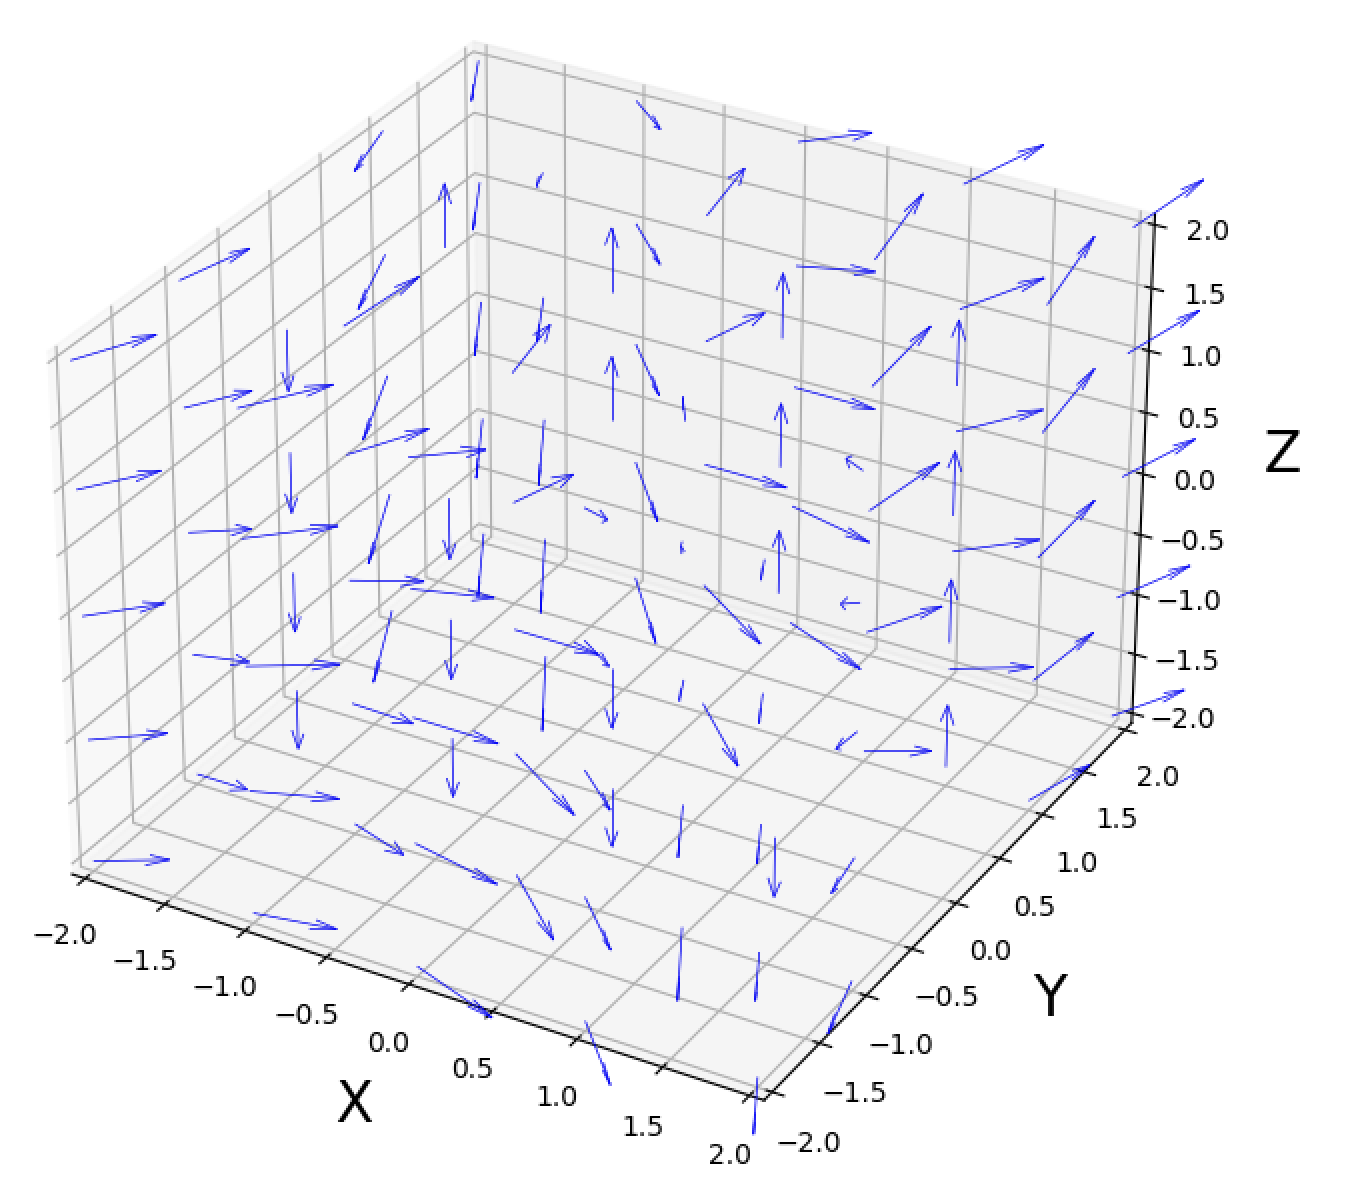
\includegraphics[width=\textwidth]{chapters/chp5_pics/5.2.4.png}
        \caption{}
        \label{fig:3d_vec_field}
    \end{subfigure}
    \caption{The path of the curves (a) with the 3D vector field plotted separately using Python (b)}
    \label{fig:comparison}
\end{figure}

\begin{solution} We'll evaluate the line integral along each segment and sum the results:
\[
\int_C \mathbf{F}\cdot d\mathbf{r} = \int_{C_1} \mathbf{F}\cdot d\mathbf{r} + \int_{C_2} \mathbf{F}\cdot d\mathbf{r} + \int_{C_3} \mathbf{F}\cdot d\mathbf{r}
\]
\noindent We will also make use of 

\[
\int_C \mathbf{F} \cdot d\mathbf{r} =  \int_a^b \left[P\frac{dx}{dt} + Q\frac{dy}{dt} + R\frac{dz}{dt}\right]\,dt.
\]

\begin{enumerate}

\item Along $C_1$ (from $A$ to $B$):
\begin{itemize}
    \item Parameterization: $\mathbf{r}(t) = t\mathbf{i} + 0\mathbf{j} + 0\mathbf{k}$, $0 \leq t \leq 1$
    \item $\frac{d\mathbf{r}}{dt} = \mathbf{i}$
    \item Along this path: $y=0$, $z=0$, and $x=t$
    \item Plug into $\mathbf{F} = (y^2)\mathbf{i} + (2xy)\mathbf{j} + (x+z)\mathbf{k}$ to get $\mathbf{F}(\mathbf{r}(t)) = (0)\mathbf{i} + (0)\mathbf{j} + (t)\mathbf{k}$
\end{itemize}
Therefore:
\begin{align*}
\int_{C_1} \mathbf{F}\cdot d\mathbf{r} &= \int_0^1 [(0)(1) + (0)(0) + (t)(0)]\,dt = 0
\end{align*}

\item Along $C_2$ (from $B$ to $C$):
\begin{itemize}
    \item Parameterization: $\mathbf{r}(t) = 1\mathbf{i} + t\mathbf{j} + 0\mathbf{k}$, $0 \leq t \leq 1$
    \item $\frac{d\mathbf{r}}{dt} = \mathbf{j}$
    \item Along this path: $x=1$, $z=0$, and $y=t$
    \item Plug into $\mathbf{F} = (y^2)\mathbf{i} + (2xy)\mathbf{j} + (x+z)\mathbf{k}$ to get $\mathbf{F}(\mathbf{r}(t)) = (t^2)\mathbf{i} + (2t)\mathbf{j} + (1)\mathbf{k}$
\end{itemize}
Therefore:
\begin{align*}
\int_{C_2} \mathbf{F}\cdot d\mathbf{r} &= \int_0^1 [(t^2)(0) + (2t)(1) + (1)(0)]\,dt \\
&= \int_0^1 2t\,dt = [t^2]_0^1 = 1
\end{align*}

\item Along $C_3$ (from $C$ to $D$):
\begin{itemize}
    \item Parameterization: $\mathbf{r}(t) = 1\mathbf{i} + 1\mathbf{j} + t\mathbf{k}$, $0 \leq t \leq 1$
    \item $\frac{d\mathbf{r}}{dt} = \mathbf{k}$
    \item Along this path: $x=1$, $y=1$, and $z=t$
    \item Plug into $\mathbf{F} = (y^2)\mathbf{i} + (2xy)\mathbf{j} + (x+z)\mathbf{k}$ to get $\mathbf{F}(\mathbf{r}(t)) = (1)\mathbf{i} + (2)(1)\mathbf{j} + (1+t)\mathbf{k}$
\end{itemize}
Therefore:
\begin{align*}
\int_{C_3} \mathbf{F}\cdot d\mathbf{r} &= \int_0^1 [(1)(0) + (2)(0) + (1+t)(1)]\,dt \\
&= \int_0^1 (1+t)\,dt = [t + \frac{t^2}{2}]_0^1 = \frac{3}{2}
\end{align*}
\end{enumerate}

The total line integral is:
\[
\int_C \mathbf{F}\cdot d\mathbf{r} = 0 + 1 + \frac{3}{2} = \frac{5}{2}
\]
\end{solution}
\end{example}
\exampleline

\subsection*{Potential Functions and Conservative Fields}

\noindent Let's now explore a special class of vector fields that yield remarkable properties. Consider a vector field $\mathbf{F}(x,y)$ defined on a simply connected domain $D$. A vector field is conservative if it can be written as the gradient of some scalar function $f(x,y)$:
\[
\mathbf{F}(x,y) = \nabla f = \frac{\partial f}{\partial x}\mathbf{i} + \frac{\partial f}{\partial y}\mathbf{j}
\]

\noindent This means that $P(x,y) = \frac{\partial f}{\partial x}$ and $Q(x,y) = \frac{\partial f}{\partial y}$. The requirement of a simply connected domain is crucial here—it ensures that any closed path can be continuously deformed to a point, which will prove essential for the path independence of our line integrals. Let's see what happens when we compute a line integral in such a field. Consider a curve $C$ lying entirely in $D$ and parameterized by $\mathbf{r}(t) = x(t)\mathbf{i} + y(t)\mathbf{j}$ from $t=a$ to $t=b$. \\

\noindent Starting with the vector field line integral:
\begin{align*}
\int_C \mathbf{F} \cdot d\mathbf{r} &= \int_C P(x,y)\,dx + Q(x,y)\,dy \\
&= \int_a^b \left[P(x(t),y(t))\frac{dx}{dt} + Q(x(t),y(t))\frac{dy}{dt}\right]\,dt
\end{align*}

\noindent Now, because $\mathbf{F}$ is conservative on our simply connected domain $D$, we can substitute $P = \frac{\partial f}{\partial x}$ and $Q = \frac{\partial f}{\partial y}$:
\begin{align*}
\int_C \mathbf{F} \cdot d\mathbf{r} &= \int_a^b \left[\frac{\partial f}{\partial x}\frac{dx}{dt} + \frac{\partial f}{\partial y}\frac{dy}{dt}\right]\,dt
\end{align*}

\noindent The key insight is recognizing that this is the chain rule for the total derivative of $f$ with respect to $t$:
\begin{align*}
\int_C \mathbf{F} \cdot d\mathbf{r} &= \int_a^b \frac{d}{dt}[f(x(t),y(t))]\,dt \\
&= f(x(b),y(b)) - f(x(a),y(a)) \\
&= f(B) - f(A)
\end{align*}

\noindent This derivation reveals the Fundamental Theorem of Line Integrals: \index{Fundamental Theorem of Line Integrals}
\[
\int_C \mathbf{F} \cdot d\mathbf{r} = f(B) - f(A)
\]
\noindent Note that this result, valid on our simply connected domain $D$, demonstrates that the line integral depends only on the endpoints $A$ and $B$, not on the particular path chosen—a powerful consequence of both the conservative nature of $\mathbf{F}$ and the simple connectivity of $D$. This looks remarkably similar to our good old friend, the Fundamental Theorem of Calculus II. \\

\noindent To build some physical intuition, think of climbing a mountain. The work (force $\times$ displacement) done against gravity (a conservative field) depends only on your starting and ending elevations, not the path you take—whether you climb straight up or take a winding trail. The simple connectivity of the domain ensures there are no ``holes" in the mountain that would force you to take fundamentally different paths (imagine if there were a bottomless pit you had to walk around). Meanwhile, the conservative nature of the field ensures that no energy is gained or lost in cycles—if you end where you started, the total work is zero, just as walking around the mountain at the same elevation requires no net work against gravity. \\

\noindent The importance of simply connected domains becomes even more profound when we delve into complex integration in Chapter 7. There, this concept forms the foundation of Cauchy's Integral Theorem and leads to the remarkable theory of complex analytic functions, where the implications of path independence reach far deeper than in the real case.

\begin{figure}[H]
    \centering
    \begin{tikzpicture}[scale=1.5]
        % Axes
        \draw[->] (-2,0) -- (2,0) node[right] {$x$};
        \draw[->] (0,-2) -- (0,2) node[above] {$y$};
        
        % Draw level curves
        \foreach \r in {0.5,1,1.5} {
            \draw[gray!50] (0,0) circle (\r);
        }
        
        % Draw two different paths
        \draw[blue, thick, ->] (-1,-1) -- (1,1);
        \draw[red, thick, ->] plot[smooth] coordinates {(-1,-1) (-0.5,0.5) (1,1)};
        
        % Add points and labels
        \fill (-1,-1) circle (1.5pt) node[below left] {$A$};
        \fill (1,1) circle (1.5pt) node[above right] {$B$};
        
        % Add potential function values
        \node[left] at (-1.15,-1) {$f=c_1$};
        \node[right] at (0.8,0.7) {$f=c_2$};
        
        % Add field vectors (with fixed spacing to avoid computation issues)
        \foreach \x in {-1.5,-1,-0.5,0,0.5,1,1.5} {
            \foreach \y in {-1.5,-1,-0.5,0,0.5,1,1.5} {
                \draw[-stealth, gray!50, thin] (\x,\y) -- +({-\x/5},{-\y/5});
            }
        }
    \end{tikzpicture}
    \caption{\textit{In a conservative field, the line integral equals the change in potential function value, regardless of path taken. Level curves of $f$ (gray circles) are perpendicular to the field vectors.}}
    \label{fig:potential_function}
    \end{figure}

\noindent This powerful result has several profound implications:

\begin{enumerate}
\item \textbf{Path Independence:} On a simply connected domain, a vector field $\mathbf{F}$ is path-independent if and only if it's conservative, meaning the line integral depends only on the endpoints $A$ and $B$, not on the path taken between them. This is because we're simply measuring the total change in the potential function $f$. Remember to check for the conservation by comparing all combinations of the partial derivatives. For a vector field in $n$ dimensions with components $F_1, F_2, ..., F_n$:
\[
\frac{\partial F_i}{\partial x_j} = \frac{\partial F_j}{\partial x_i} \quad \text{for all } i,j \in \{1,...,n\}, \, i \neq j
\]
For example, in three dimensions ($n=3$ dimensions), this gives us:
\[
\frac{\partial P}{\partial y} = \frac{\partial Q}{\partial x}, \quad
\frac{\partial P}{\partial z} = \frac{\partial R}{\partial x}, \quad
\frac{\partial Q}{\partial z} = \frac{\partial R}{\partial y}
\]

    \item \textbf{Closed Paths:} If $C$ is a closed path (where $A=B$), then:
    \[
    \oint_C \mathbf{F} \cdot d\mathbf{r} = f(A) - f(A) = 0
    \]
    The circle in the integral symbol reminds us we're integrating around a closed loop.
    
    \item \textbf{Equipotential Curves:} Along any curve where $f$ is constant (level curves of $f$), the line integral is zero because there's no change in potential.
\end{enumerate}

\noindent In physics, this theorem explains why conservative forces (like gravity) do work that depends only on initial and final positions, not the path taken. The potential function $f$ might represent Gravitational potential energy, Electric potential in an electrostatic field, Pressure potential in a static fluid, and more. \\

\noindent This connection between conservative vector fields and potential functions provides both computational simplification and deep physical insight. When we can identify a potential function, complicated line integral calculations reduce to simple evaluation at endpoints. \\

\noindent Let's take some examples of these concepts now:

\exampleline
\begin{example}
For each of the following vector fields:
\begin{itemize}
    \item Check if the field is conservative
    \item If conservative, find its potential function
    \item Evaluate the given line integral
\end{itemize}
\noindent Vector fields and regions:

\begin{enumerate}
\item $\mathbf{F}_1(x,y) = (3x^2 + y)\mathbf{i} + (x + 4y^3)\mathbf{j}$ on $\mathbb{R}^2$\\
Evaluate $\oint_C \mathbf{F}_1\cdot d\mathbf{r}$ along the closed curve $C$ shown:

\begin{center}
\begin{tikzpicture}[scale=1]
    % Draw axes
    \draw[->] (-2,0) -- (4,0) node[right] {$x$};
    \draw[->] (0,-1) -- (0,2.2) node[above] {$y$};
    
    % Draw a closed curve (ellipse)
    \draw[thick, blue] plot [smooth cycle, tension=1] coordinates { 
        (-1,1) (1,2) (3,1) (1,0) 
    };
    
    % Label the curve
    \node at (2.3,1.3) {$C$};
\end{tikzpicture}
\end{center}

\item $\mathbf{F}_2(x,y) = e^y\mathbf{i} + xe^y\mathbf{j}$ on $\mathbb{R}^2$\\
Evaluate $\int_C \mathbf{F}_2\cdot d\mathbf{r}$ from $A(0,0)$ to $B(1,2)$ along the curve shown:

\begin{center}
\begin{tikzpicture}[scale=1.5]
% Draw axes
\draw[->] (-0.5,0) -- (2,0) node[right] {$x$};
\draw[->] (0,-0.5) -- (0,3) node[above] {$y$};
% Draw a wild line
\draw[thick, red, ->] (0,0) .. controls (0.2,1.5) and (0.8,1.5) .. (1,2)
.. controls (1.2,2.5) and (0.5,2.8) .. (0,2)
.. controls (-0.5,1.2) and (1.5,1.8) .. (1.5,0.5)
.. controls (1.5,-0.3) and (0.5,-0.3) .. (0.5,0.5)
.. controls (0.5,1.3) and (1.5,1.3) .. (1.5,0.5)
.. controls (1.5,-0.1) and (1.1,-0.1) .. (1,0.2)
.. controls (0.9,0.5) and (1.1,0.5) .. (1,0.8)
.. controls (0.9,1.1) and (1.1,1.1) .. (1,1.4)
.. controls (0.9,1.7) and (1.1,1.7) .. (1,2);
% Label points A and B
\filldraw [black] (0,0) circle (1pt) node[anchor=north east] {$A(0,0)$};
\filldraw [black] (1,2) circle (1pt) node[anchor=south west] {$B(1,2)$};
\end{tikzpicture}
\end{center}

\item $\mathbf{F}_3(x,y) = \frac{-y}{x^2 + y^2}\mathbf{i} + \frac{x}{x^2 + y^2}\mathbf{j}$ on $\mathbb{R}^2\setminus\{(0,0)\}$\\
Evaluate $\oint_C \mathbf{F}_3\cdot d\mathbf{r}$ along any circle centered at the origin.
\end{enumerate}

\begin{solution}
\begin{enumerate}
\item For $\mathbf{F}_1$:
    \begin{itemize}
        \item Check if conservative by comparing partial derivatives:
        \[
        \frac{\partial P}{\partial y} = 1 = \frac{\partial Q}{\partial x}
        \]
        \item Since these are equal and the domain is simply connected, $\mathbf{F}_1$ is conservative
        \item Find potential function by integrating $P$ with respect to $x$:
        \begin{align*}
        f(x,y) &= \int (3x^2 + y)\,dx = x^3 + xy + g(y) \\
        \frac{\partial f}{\partial y} &= x + g'(y) = x + 4y^3 \quad \text{(comparing with $Q$)} \\
        g(y) &= y^4 + C
        \end{align*}
        \item Therefore, $f(x,y) = x^3 + xy + y^4 + C$
        \item For any closed curve over a conservative vector: $\oint_C \mathbf{F}_1\cdot d\mathbf{r} = 0$
    \end{itemize}

    \item For $\mathbf{F}_2$:
    \begin{itemize}
        \item Check partial derivatives:
        \[
        \frac{\partial P}{\partial y} = e^y = \frac{\partial Q}{\partial x}
        \]
        \item Field is conservative on $\mathbb{R}^2$ (simply connected domain)
        \item Find potential function:
        \begin{align*}
        f(x,y) &= \int e^y\,dx = xe^y + g(y) \\
        \frac{\partial f}{\partial y} &= xe^y + g'(y) = xe^y \quad \text{(comparing with $Q$)} \\
        g(y) &= C
        \end{align*}
        \item Therefore, $f(x,y) = xe^y + C$
        \item Line integral from $A(0,0)$ to $B(1,2)$:
        \begin{align*}
        \int_C \mathbf{F}_2\cdot d\mathbf{r} &= f(B) - f(A) \\
        &= [f(1,2)] - [f(0,0)] \\
        &= [(1)e^2 + C] - [(0)e^0 + C] \\
        &= e^2 + C - C \\
        &= e^2
        \end{align*}
        Note how the constant $C$ cancels in the difference.
    \end{itemize}


    \item For $\mathbf{F}_3$:
    \begin{itemize}
        \item Check partial derivatives:
        \begin{align*}
        \frac{\partial P}{\partial y} &= \frac{-x^2 + y^2}{(x^2 + y^2)^2} \\
        \frac{\partial Q}{\partial x} &= \frac{-x^2 + y^2}{(x^2 + y^2)^2}
        \end{align*}
        \item Although partial derivatives are equal, domain is not simply connected (origin removed)
        \item Therefore $\mathbf{F}_3$ is not conservative
        \item For a circle of radius $r$ centered at origin, parameterize on $t \in [0,2\pi]$ using:
        \[
        x = r\cos\theta, \quad y = r\sin\theta
        \]
        \item Calculating $\mathbf{F}_3 \cdot d\mathbf{r}$:
        \begin{align*}
            \mathbf{F}_3 &= \frac{-y}{r^2}\mathbf{i} + \frac{x}{r^2}\mathbf{j} = \frac{-\sin\theta}{r}\mathbf{i} + \frac{\cos\theta}{r}\mathbf{j} \\
            d\mathbf{r} &= \frac{dx}{d\theta}d\theta\mathbf{i} + \frac{dy}{d\theta}d\theta\mathbf{j} = -r\sin\theta d\theta\mathbf{i} + r\cos\theta d\theta\mathbf{j}
        \end{align*}
        \item Taking the dot product:
        \begin{align*}
            \mathbf{F}_3 \cdot d\mathbf{r} &= \left(\frac{-\sin\theta}{r}\right)(-r\sin\theta d\theta) + \left(\frac{\cos\theta}{r}\right)(r\cos\theta d\theta) \\
            &= \sin^2\theta d\theta + \cos^2\theta d\theta \\
            &= (\sin^2\theta + \cos^2\theta)d\theta = d\theta
        \end{align*}
        \item Therefore, for any circle centered at origin:
        \[
        \oint_C \mathbf{F}_3\cdot d\mathbf{r} = \int_0^{2\pi} 1\,d\theta = 2\pi
        \]
        regardless of the radius $r$
    \end{itemize}

\end{enumerate}
\end{solution}
\end{example}
\exampleline

\exampleline
\begin{example}
Show that \( \mathbf{F}(x,y,z) = \langle yz, \, xz, \, xy \rangle \) is conservative and find a potential function.

\begin{solution}
We check: \( \partial P/\partial y = z = \partial Q/\partial x \), \( \partial P/\partial z = y = \partial R/\partial x \), \( \partial Q/\partial z = x = \partial R/\partial y \). All conditions are satisfied, so \( \mathbf{F} \) is conservative.\\ \\
\noindent To find \( f \), integrate \( P = yz \) with respect to \( x \):
\[ f(x,y,z) = xyz + g(y,z). \]
Differentiate with respect to \( y \): \( f_y = xz + g_y(y,z) \). Setting this equal to \( Q = xz \) gives \( g_y = 0 \), so \( g(y,z) = h(z) \).\\ \\
\noindent Differentiate with respect to \( z \): \( f_z = xy + h'(z) \). Setting this equal to \( R = xy \) gives \( h'(z) = 0 \), so \( h(z) = C \).\\ \\
\noindent Therefore \( f(x,y,z) = xyz + C \).
\end{solution}
\end{example}
\exampleline


\newpage

\lecture{Green's Theorem} \index{Green's Theorem} \index{Flux}

\noindent The relationship between derivatives and integrals stands as one of the most profound insights in mathematics. We've seen this connection in various forms: the Fundamental Theorem of Calculus linking derivatives to single integrals, and the relationship between partial derivatives and multiple integrals in higher dimensions. Now we explore another manifestation of this deep connection—Green's Theorem—which relates line integrals around a closed curve to double integrals over the region it encloses. This relationship not only provides computational power but also reveals fundamental properties of vector fields and their behavior in the plane. \\

\noindent The path to understanding Green's Theorem will leverage several powerful tools from our mathematical arsenal. The Mean Value Theorem will help us analyze vector field behavior over small intervals, while Taylor's Theorem will allow us to approximate vector components with increasing accuracy. These classical results, combined with careful limiting arguments, will reveal how local vector field properties accumulate to create global patterns of circulation and flux, which refers to the flow of the vector field through a surface. \\

\noindent Our journey begins with an intuitive understanding through fluid flow, moves through rigorous mathematical development, and culminates in a theorem that bridges boundary behavior with interior properties. Just as the Fundamental Theorem of Calculus shows how differentiation and integration are inverse processes, Green's Theorem will demonstrate how boundary circulation captures the cumulative effect of interior rotation. This lecture represents an important leap in mathematical formalism for advanced theorems that you may not have encountered before. Don't get caught up too much in the detail, but stop to appreciate how we lay out the architecture. 


\subsection*{Motivation and Mathematical Foundation}

\noindent Before diving into the mathematics, let's build some intuition. Imagine a lake with a current described by a vector field $\mathbf{F}(x,y) = P(x,y)\mathbf{i} + Q(x,y)\mathbf{j}$. When studying this flow, we might be interested in two fundamental quantities:

\begin{itemize}
    \item The circulation of the water around the lake's boundary
    \item How much the water rotates or ``swirls" at each point inside the lake
\end{itemize}

\noindent The first quantity measures boundary behavior through a line integral $\oint_C \mathbf{F}\cdot d\mathbf{r}$, while the second examines interior rotation through derivatives $\frac{\partial Q}{\partial x} - \frac{\partial P}{\partial y}$. Green's Theorem reveals that these seemingly different measurements are intimately connected—the total circulation around the boundary exactly equals the sum of all the interior rotation. \\

\noindent To understand Green's Theorem from a rigorous mathematical perspective, let's begin to build the framework piece by piece using tools we know. Consider a simple closed curve $C$ with four constituent parts $C_1,...,C_4$ in the plane, oriented counterclockwise, that bounds a region $D$. We can think about this curve in two complementary ways:

\begin{enumerate}
    \item As the boundary where we might evaluate a line integral
    \item As the edge of a region where we might compute a double integral
\end{enumerate}

\begin{figure}[H]
\centering
\begin{tikzpicture}
    % Draw axes
    \draw[->] (0,0) -- (5,0) node[right] {$x$};
    \draw[->] (0,0) -- (0,5) node[above] {$y$};
    
    % Draw region D with modified boundary
    \begin{scope}
        \clip (0.8,0) rectangle (3.2,4);
        \fill[blue!30] (1,0) .. controls (1.5,0.8) and (2.5,0.8) .. (3,0)  % C₁
            -- (3,3.5) % C₂
            .. controls (2.5,3.2) and (1.5,3.2) .. (1,3.5) % C₃
            -- (1,0); % C₄
    \end{scope}
    
    % Draw colored boundary segments with arrows for counterclockwise direction
    \draw[red, thick, ->] (1,0) .. controls (1.5,0.8) and (2.5,0.8) .. (3,0);    % C₁
    \draw[green, thick, ->] (3,0) -- (3,3.5);  % C₂
    \draw[yellow, thick, ->] (3,3.5) .. controls (2.5,3.2) and (1.5,3.2) .. (1,3.5); % C₃
    \draw[green, thick, ->] (1,3.5) -- (1,0);  % C₄
    
    % Add labels
    \node at (2,2) {$D$};
    \node[below] at (1,0) {$a$};
    \node[below] at (3,0) {$b$};
    \node[below] at (2,0.55) {$C_1$};
    \node[right] at (3,1.75) {$C_2$};
    \node[above] at (2,3.3) {$C_3$};
    \node[left] at (1,1.75) {$C_4$};
\end{tikzpicture}

\caption{\textit{A region $D$ bounded by a curve $C = C_1 + C_2 + C_3 + C_4$. We can begin to heuristically see the relationship between the line integral and the double integral.}}
\label{fig:green}
\end{figure}

\noindent Let's explore why these perspectives might be related. Consider breaking our region into tiny rectangles with sides $\Delta x$ and $\Delta y$. For each rectangle:

\begin{itemize}
    \item The line integral around its boundary involves terms like $P\Delta x$ and $Q\Delta y$
    \item The double integral over its area involves terms like $\frac{\partial Q}{\partial x}\Delta x\Delta y$ and $\frac{\partial P}{\partial y}\Delta x\Delta y$
\end{itemize}

\noindent This suggests a possible connection between:
\[
\text{Boundary Terms: } P\Delta x + Q\Delta y 
\]
and
\[
\text{Area Terms: } \left(\frac{\partial Q}{\partial x} - \frac{\partial P}{\partial y}\right)\Delta x\Delta y
\]

\begin{figure}[H]
\centering

\begin{tikzpicture}[scale=3]
    % Draw main axes
    \draw[->] (0,0) -- (1.5,0) node[right] {$x$};
    \draw[->] (0,0) -- (0,1.5) node[above] {$y$};

    % Draw rectangle (differential element)
    \draw[very thick] (0.6,0.6) rectangle (1.2,1.2);

    % Add dots at vertices
    \fill (0.6,0.6) circle (0.7pt);  % (x,y)
    \fill (1.2,0.6) circle (0.7pt);  % (x+dx,y)
    \fill (0.6,1.2) circle (0.7pt);  % (x,y+dy)

    % Label vertices
    \node[below right] at (0.2,0.6) {$(x,y)$};
    \node[below right, xshift=2] at (1.2,0.6) {$(x+dx,y)$};
    \node[above right, yshift=2] at (0.2,1.2) {$(x,y+dy)$};

    % Add vector field components with arrows and separate labels
    \draw[-stealth, red] (0.8,0.6) -- (0.8,0.77);
    \node[right, xshift=1] at (0.8,0.685) {$Qdy$};
    
\draw[-stealth, blue] (0.6,0.8) -- (0.77,0.8);
    \node[above, yshift=1] at (0.75,0.8) {$Pdx$};

    % Label differential measurements
    \draw[|<->|] (0.6,0.5) -- (1.2,0.5) node[midway,below] {$dx$};
    \draw[|<->|] (1.3,0.6) -- (1.3,1.2) node[midway,right] {$dy$};
\end{tikzpicture}
\caption{\textit{Differential element showing contributions of a vector field $(P,Q)$ to the line integral around the boundary of the rectangular area element $dxdy$.}}
\label{fig:differential_element}
\end{figure}

\noindent To formalize this intuition, let's examine what happens when we sum the line integral contributions around a single small rectangle with vertices at $(x,y)$, $(x+\Delta x,y)$, $(x+\Delta x,y+\Delta y)$, and $(x,y+\Delta y)$:

\begin{align*}
\oint_{\text{rect}} P\,dx + Q\,dy &= \int_{x}^{x+\Delta x} P(s,y)\,ds + \int_{y}^{y+\Delta y} Q(x+\Delta x,t)\,dt \\
&\quad - \int_{x+\Delta x}^{x} P(s,y+\Delta y)\,ds - \int_{y+\Delta y}^{y} Q(x,t)\,dt.
\end{align*}

\noindent Using the Mean Value Theorem and Taylor's Theorem, we expand $Q(x+\Delta x, y)$ and $P(x, y+\Delta y)$ around $(x, y)$:

\begin{align*}
Q(x+\Delta x,y) &= Q(x,y) + \frac{\partial Q}{\partial x}\Delta x + O(\Delta x^2), \\
P(x,y+\Delta y) &= P(x,y) + \frac{\partial P}{\partial y}\Delta y + O(\Delta y^2).
\end{align*}

\noindent For higher-order terms ($O(\Delta x^2)$, for example), note that these terms vanish in the limit as $\Delta x, \Delta y \to 0$ due to their smaller magnitude compared to $\Delta x$ or $\Delta y$. After careful algebraic manipulation, the line integral around the rectangle simplifies to:

\[
\oint_{\text{rect}} P\,dx + Q\,dy = \left(\frac{\partial Q}{\partial x} - \frac{\partial P}{\partial y}\right)\Delta x\Delta y + O(\Delta x^2\Delta y + \Delta x\Delta y^2).
\]

\noindent Here, $\Delta x\Delta y$ represents the leading-order contribution proportional to the area of the rectangle, while the higher-order terms vanish faster than $\Delta x\Delta y$ as $\Delta x, \Delta y \to 0$. This dominant term transitions to the differential $dx\,dy$ in the integral when taking the limit over all rectangles.

\bigskip

\noindent The key insight is this: if we partition the entire region $D$ into such small rectangles and sum their contributions, the following occurs:

\begin{itemize}
    \item Interior edges cancel in pairs, as they are traversed in opposite directions.
    \item Only the boundary edges survive, forming the boundary $\partial D$ of the region $D$.
    \item The sum of area terms provides an approximation to the double integral over $D$.
\end{itemize}

\bigskip

\noindent Taking the limit as the partition becomes infinitely fine, let the partition consist of $n$ rectangles, each with area $\Delta A_i = \Delta x_i\Delta y_i$. For each rectangle $R_i$, the local line integral can be expressed as:

\[
\oint_{\partial R_i} P\,dx + Q\,dy = \left(\frac{\partial Q}{\partial x} - \frac{\partial P}{\partial y}\right)\Delta A_i + O(\Delta x_i^2\Delta y_i + \Delta x_i\Delta y_i^2).
\]

\noindent Summing over all rectangles, we obtain:

\begin{align*}
\sum_{i=1}^n \oint_{\partial R_i} P\,dx + Q\,dy &= \sum_{i=1}^n \left[\left(\frac{\partial Q}{\partial x} - \frac{\partial P}{\partial y}\right)\Delta A_i + O(\Delta x_i^2\Delta y_i + \Delta x_i\Delta y_i^2)\right] \\[1em]
&= \sum_{i=1}^n \left(\frac{\partial Q}{\partial x} - \frac{\partial P}{\partial y}\right)\Delta A_i + \sum_{i=1}^n O(\Delta x_i^2\Delta y_i + \Delta x_i\Delta y_i^2).
\end{align*}

\noindent Let $\delta = \max_i\{\Delta x_i, \Delta y_i\}$ denote the mesh size of the partition. The error term is then bounded by:
\[
\left|\sum_{i=1}^n O(\Delta x_i^2\Delta y_i + \Delta x_i\Delta y_i^2)\right| \leq M\delta \text{Area}(D),
\]
for some constant $M$. As $\delta \to 0$, the error term vanishes, leaving:
\[
\lim_{\delta \to 0} \sum_{i=1}^n \oint_{\partial R_i} P\,dx + Q\,dy = \lim_{\delta \to 0} \sum_{i=1}^n \left(\frac{\partial Q}{\partial x} - \frac{\partial P}{\partial y}\right)\Delta A_i.
\]

\noindent On the left-hand side, the sum of line integrals reduces to the line integral around the boundary of the region:
\[
\oint_{\partial D} P\,dx + Q\,dy.
\]
On the right-hand side, the Riemann sum transitions to the double integral over $D$:
\[
\lim_{\delta \to 0} \sum_{i=1}^n \left(\frac{\partial Q}{\partial x} - \frac{\partial P}{\partial y}\right)\Delta A_i = \iint_D \left(\frac{\partial Q}{\partial x} - \frac{\partial P}{\partial y}\right)\,dA.
\]

\bigskip

\noindent Through this limiting process, the local relationships derived for small rectangles extend to the entire region $D$. As the partition becomes infinitely fine ($\delta \to 0$), the sum of approximations converges to exact values: the line integral around the boundary of $D$ is precisely balanced by the double integral of the curl over the region. This establishes \textbf{Green's Theorem}:
\[
\oint_{\partial D} \mathbf{F} \cdot d\mathbf{r} = \oint_{\partial D} P\,dx + Q\,dy = \iint_D \left(\frac{\partial Q}{\partial x} - \frac{\partial P}{\partial y}\right)\,dA.
\]
\noindent Here \( \partial D \) is traversed counterclockwise (positive orientation), and \( D \) must be simply connected.\\ \\

\noindent Green's Theorem also has a \textit{flux form}. If \( \mathbf{F} = P\mathbf{i} + Q\mathbf{j} \), then:
\[
\oint_{\partial D} (P \, dy - Q \, dx) = \iint_D \left(\frac{\partial P}{\partial x} + \frac{\partial Q}{\partial y}\right) dA = \iint_D \operatorname{div} \mathbf{F} \, dA.
\]
The circulation form generalizes to Stokes' Theorem; the flux form generalizes to the Divergence Theorem.\\ \\
\noindent A useful consequence of Green's Theorem is the \textbf{area formula}:
\[
A = \frac{1}{2}\oint_C (x \, dy - y \, dx),
\]
which computes the area of the region enclosed by a simple closed curve \( C \).\\ \\
\noindent This theorem stands as a fundamental bridge between different types of integration, much like how the Fundamental Theorem of Calculus I connects derivatives and integrals in single-variable calculus. What makes this theorem even more remarkable is that it solves so many physics problems with surprisingly few physical assumptions. As the saying goes, the potency of a law is the strength of what it proves divided by what it assumes. \\

\noindent We can now substitute line integrals for double integrals wherever it proves advantageous—a frequent and powerful simplification! Do you see anything interesting about the integrand? Anything that connects to Chapter 1 vector concepts? We will soon make an important generalization of Green's Theorem, but as an exercise, try to see if you can adjust this formula for any dimension $n$. \\

\noindent Let's consider one more intuitive example. Imagine a region enclosed by a smooth, oriented curve $C$, as shown in the diagram. Inside this curve, we have several small, uniformly distributed loops, all oriented in the same direction. Each of these loops can be thought of as representing a local rotational field or a ``microscopic circulation" at each point in the region. The arrows on the boundary $C$ indicate the macroscopic circulation along the curve's orientation. By Green's Theorem, the total circulation along $C$ is equal to the sum of these individual microscopic rotations, effectively connecting the behavior of the field inside the region to its boundary.


\exampleline
\begin{example}
Consider the vector field $\mathbf{F}(x,y) = (x^3y^2)\mathbf{i} + (x^2y^3)\mathbf{j}$. Evaluate $\oint_C \mathbf{F}\cdot d\mathbf{r}$, where $C$ is the triangle with vertices at $(0,0)$, $(1,0)$, and $(0,1)$, oriented counterclockwise.

\begin{solution}
We'll solve this two ways: first directly using the line integral, and then using Green's Theorem.

\begin{enumerate}
\item \textbf{Method 1: Direct Line Integral}

Split the boundary \(C\) into three segments: 
\begin{itemize}
    \item \(C_1\): From \((0,0)\) to \((1,0)\),
    \item \(C_2\): From \((1,0)\) to \((0,1)\),
    \item \(C_3\): From \((0,1)\) to \((0,0)\).
\end{itemize}
Let's crunch these now (even though if you look at the vector field you may already know the answer...)
\begin{enumerate}
\item \(C_1\): From \((0,0)\) to \((1,0)\)
Parameterize \(C_1\):
\[
\mathbf{r}_1(t) = (t, 0), \quad 0 \leq t \leq 1, \quad \text{so } \frac{d\mathbf{r}_1}{dt} = (1, 0).
\]
Evaluate \(\mathbf{F} \cdot d\mathbf{r}\) along \(C_1\):
\[
\mathbf{F}(x,y) = (x^3y^2, x^2y^3), \quad \mathbf{F}(\mathbf{r}_1(t)) = (t^3 \cdot 0^2, t^2 \cdot 0^3) = (0, 0).
\]
Thus:
\[
\int_{C_1} \mathbf{F} \cdot d\mathbf{r} = \int_0^1 (0)(1) + (0)(0)\,dt = 0.
\]

\item \(C_2\): From \((1,0)\) to \((0,1)\)
Parameterize \(C_2\):
\[
\mathbf{r}_2(t) = (1-t, t), \quad 0 \leq t \leq 1, \quad \frac{d\mathbf{r}_2}{dt} = (-1, 1).
\]
Evaluate \(\mathbf{F} \cdot d\mathbf{r}\) along \(C_2\):
\[
\mathbf{F}(x,y) = (x^3y^2, x^2y^3), \quad \mathbf{F}(\mathbf{r}_2(t)) = ((1-t)^3t^2, (1-t)^2t^3).
\]
\[
\mathbf{F} \cdot \frac{d\mathbf{r}_2}{dt} = ((1-t)^3t^2)(-1) + ((1-t)^2t^3)(1).
\]
Simplify:
\[
\mathbf{F} \cdot \frac{d\mathbf{r}_2}{dt} = -t^2(1-t)^3 + t^3(1-t)^2.
\]
Integrate:
\[
\int_{C_2} \mathbf{F} \cdot d\mathbf{r} = \int_0^1 \big(-t^2(1-3t+3t^2-t^3) + t^3(1-2t+t^2)\big)\,dt.
\]
Expand:
\[
-t^2(1 - 3t + 3t^2 - t^3) = -t^2 + 3t^3 - 3t^4 + t^5,
\]
\[
t^3(1 - 2t + t^2) = t^3 - 2t^4 + t^5.
\]
Combine terms:
\[
\int_{C_2} \mathbf{F} \cdot d\mathbf{r} = \int_0^1 \big(-t^2 + 4t^3 - 5t^4 + 2t^5\big)\,dt.
\]
Integrate term by term:
\[
\int_0^1 \mathbf{F} \cdot d\mathbf{r} = \left[-\frac{t^3}{3} + t^4 - \frac{5t^5}{5} + \frac{2t^6}{6}\right]_0^1 = -\frac{1}{3} + 1 - 1 + \frac{1}{3} = 0.
\]

\item \(C_3\): From \((0,1)\) to \((0,0)\)
Parameterize \(C_3\):
\[
\mathbf{r}_3(t) = (0, 1-t), \quad 0 \leq t \leq 1, \quad \frac{d\mathbf{r}_3}{dt} = (0, -1).
\]
Evaluate \(\mathbf{F} \cdot d\mathbf{r}\) along \(C_3\):
\[
\mathbf{F}(x,y) = (x^3y^2, x^2y^3), \quad \mathbf{F}(\mathbf{r}_3(t)) = (0^3(1-t)^2, 0^2(1-t)^3) = (0, 0).
\]
Thus:
\[
\int_{C_3} \mathbf{F} \cdot d\mathbf{r} = \int_0^1 (0)(0) + (0)(-1)\,dt = 0.
\]

The total line integral is:
\[
\oint_C \mathbf{F} \cdot d\mathbf{r} = \int_{C_1} \mathbf{F} \cdot d\mathbf{r} + \int_{C_2} \mathbf{F} \cdot d\mathbf{r} + \int_{C_3} \mathbf{F} \cdot d\mathbf{r} = 0 + 0 + 0 = 0.
\]
\end{enumerate}

\item \textbf{Method 2: Green's Theorem}

Using Green's Theorem:
\[
\oint_C \mathbf{F} \cdot d\mathbf{r} = \iint_D \left(\frac{\partial Q}{\partial x} - \frac{\partial P}{\partial y}\right)\,dA.
\]
Compute:
\[
\frac{\partial Q}{\partial x} = 2xy^3, \quad \frac{\partial P}{\partial y} = 2x^3y, \quad \frac{\partial Q}{\partial x} - \frac{\partial P}{\partial y} = 2xy^3 - 2x^3y.
\]

Set up the integral:
\[
\iint_D (2xy^3 - 2x^3y)\,dA = \int_0^1 \int_0^{1-x} (2xy^3 - 2x^3y)\,dy\,dx.
\]
Evaluate the inner integral:
\[
\int_0^{1-x} (2xy^3 - 2x^3y)\,dy = \left[2x\frac{y^4}{4} - 2x^3\frac{y^2}{2}\right]_0^{1-x}.
\]
Substituting \(y = 1-x\):
\[
\int_0^{1-x} (2xy^3 - 2x^3y)\,dy = \frac{x(1-x)^4}{2} - x^3(1-x)^2.
\]
Finally, integrate with respect to \(x\):
\[
\int_0^1 \left(\frac{x(1-x)^4}{2} - x^3(1-x)^2\right)\,dx = 0.
\]

\end{enumerate}

Both methods confirm:
\[
\oint_C \mathbf{F} \cdot d\mathbf{r} = 0.
\]
\end{solution}
\end{example}
\exampleline

\noindent \noindent Now we don't always have to transform line integrals into double integrals. We can use Green's Theorem in both directions. This bidirectional relationship provides a powerful computational tool, allowing us to choose the most elegant solution path. Sometimes, seemingly complex double integrals can be dramatically simplified by recognizing that they represent the integrand of some vector field's differentiated component's differences—a pattern that transforms our volume calculation into a boundary computation.

\exampleline
\begin{example}
In computational fluid dynamics, understanding vorticity patterns often requires calculating complex volume integrals. Consider a basin modeled by the region $D$ bounded by $y=x^2$ and $y=2-x^2$ for $x \in [-1,1]$. A vorticity field in this basin is given by $f(x,y) = xe^y - y\cos(x)$. Our task is to calculate the total vorticity by evaluating $\iint_D f(x,y)\,dA$.

\begin{figure}[H]
\centering
\begin{tikzpicture}[scale=2]
    % Draw axes
    \draw[->] (-1.5,0) -- (1.5,0) node[right] {$x$};
    \draw[->] (0,0) -- (0,2.5) node[above] {$y$};
    
    % Draw parabolas and fill region
    \draw[thick, blue] plot[domain=-1:1] (\x,{2-\x*\x}) node[right] {};
    \draw[thick, blue] plot[domain=-1:1] (\x,{\x*\x}) node[right] {};
    \fill[blue!10] plot[domain=-1:1] (\x,{\x*\x}) -- plot[domain=1:-1] (\x,{2-\x*\x});
    
    % Add vector field visualization with smaller, denser arrows
    \foreach \x in {-0.75,-0.5,-0.25,0,0.25,0.5,0.75} {
        \foreach \y in {0.5,0.75,1,1.25,1.5} {
            \pgfmathparse{(\y < 2-\x*\x-0.1) && (\y > \x*\x+0.1)}
            \ifnum\pgfmathresult=1
                \draw[->, blue!40] (\x,\y) arc (0:270:0.06);
            \fi
        }
    }
    
    
    % Add labels and reference points
    \node at (0,1) {$D$};
    \fill (1,1) circle (0.5pt) node[right] {\small $(1,1)$};
    \fill (-1,1) circle (0.5pt) node[left] {\small $(-1,1)$};
    

\end{tikzpicture}
\caption{\textit{The basin region $D$ bounded by $y=x^2$ and $y=2-x^2$. Blue arrows indicate local vorticity patterns, demonstrating the symmetric flow structure about the vertical axis. This visualization helps us understand why the total vorticity integrates to $8[\sin(1) - \cos(1)]$.}}
\label{fig:flow_basin}
\end{figure}

\begin{solution}
\noindent Rather than tackle this double integral directly, we can exploit the structure of Green's Theorem to transform our area computation into a boundary analysis:

\begin{enumerate}
\item \textbf{Recognition of Pattern}\\
Our vorticity field $f(x,y) = xe^y - y\cos(x)$ mirrors the curl formula $\frac{\partial Q}{\partial x} - \frac{\partial P}{\partial y}$ in Green's Theorem:
\[
\iint_D \left(\frac{\partial Q}{\partial x} - \frac{\partial P}{\partial y}\right)\,dA = \oint_{\partial D} P\,dx + Q\,dy
\]

\item \textbf{Construction of Potential Functions}\\
We identify functions $P$ and $Q$ satisfying our pattern:
\begin{align*}
P(x,y) &= -xe^y \\
Q(x,y) &= -y\sin(x)
\end{align*}

Verification through partial derivatives:
\begin{align*}
\frac{\partial Q}{\partial x} &= -y\cos(x) \\
-\frac{\partial P}{\partial y} &= xe^y
\end{align*}
Therefore: $\frac{\partial Q}{\partial x} - \frac{\partial P}{\partial y} = xe^y - y\cos(x) = f(x,y)$

\item \textbf{Boundary Analysis}\\
Our region's boundary $\partial D$ comprises:
\begin{itemize}
   \item Upper curve: $y = 2-x^2$, traversed from $x = -1$ to $x = 1$
   \item Lower curve: $y = x^2$, traversed from $x = 1$ to $x = -1$
\end{itemize}

\item \textbf{Line Integral Formulation}\\
Along the upper curve ($y = 2-x^2$):
\[
\int_{-1}^1 [-xe^{2-x^2} + 2x(2-x^2)\sin(x)]\,dx
\]

Along the lower curve ($y = x^2$):
\[
\int_{-1}^1 [xe^{x^2} + 2x^3\sin(x)]\,dx
\]

Combining yields:
\[
\int_{-1}^1 [x(e^{x^2} - e^{2-x^2}) + 4x\sin(x)]\,dx
\]

\item \textbf{Symmetry Exploitation}\\
Two key observations simplify our computation:
\begin{itemize}
   \item $x(e^{x^2} - e^{2-x^2})$ is odd on $[-1,1]$, contributing zero to the integral
   \item $4x\sin(x)$ exhibits even symmetry, allowing reduction to $[0,1]$
\end{itemize}

Therefore:
\begin{align*}
\iint_D f(x,y)\,dA &= 8\int_0^1 x\sin(x)\,dx \\
&= 8[\sin(1) - \cos(1)] \\
&\approx 2.4096
\end{align*}
\end{enumerate}

\noindent \textbf{Physical Interpretation:}
The final value of approximately $2.4096$ reveals several key insights about our vorticity field:
\begin{itemize}
   \item The positive result indicates a net counterclockwise rotation in the basin
   \item The moderate magnitude suggests balanced vorticity distribution
   \item The symmetric basin geometry is reflected in our integration technique
   \item Local rotational effects combine to produce measurable global circulation
\end{itemize}

\end{solution}
\end{example}
\exampleline


\subsection*{Big $O$ Notation}

\noindent When we work with limits and approximations in calculus, we often encounter situations where we want to describe how quickly certain terms become negligible as a variable approaches zero. Big $O$ notation provides a precise language for describing these behaviors. \\

\noindent In its simplest form, when we write $f(x) = O(g(x))$ as $x \to a$, we mean that the function $f(x)$ grows no faster than $g(x)$ near $a$. More precisely, there exist constants $M > 0$ and $\delta > 0$ such that:
\[
|f(x)| \leq M|g(x)| \quad \text{whenever } |x-a| < \delta
\]

\noindent For example, in our analysis of Green's Theorem, we encountered terms like:
\[
O(\Delta x^2\Delta y + \Delta x\Delta y^2)
\]
This notation tells us that as $\Delta x$ and $\Delta y$ approach zero, these "error terms" become negligible much faster than the main terms ($\Delta x\Delta y$) in our approximation. \\

\noindent A powerful illustration of this notation appears in the limit definition of the derivative. Consider finding $\frac{d}{dx}(x^n)$ using first principles:
\begin{align*}
\frac{d}{dx}(x^n) &= \lim_{h \to 0} \frac{(x+h)^n - x^n}{h} \\
&= \lim_{h \to 0} \frac{x^n + nx^{n-1}h + \frac{n(n-1)}{2}x^{n-2}h^2 + O(h^3) - x^n}{h} \\
&= \lim_{h \to 0} \left(nx^{n-1} + \frac{n(n-1)}{2}x^{n-2}h + O(h^2)\right) \\
&= nx^{n-1}
\end{align*}

\noindent Here, $O(h^3)$ captures all terms with powers of $h$ greater than 2 in the binomial expansion, and after dividing by $h$, these terms become $O(h^2)$. As $h \to 0$, these higher-order terms vanish, leaving us with our familiar result. \\

\noindent Think of Big $O$ notation as a way of classifying the "speed" at which functions approach zero:
\begin{itemize}
   \item $O(\Delta x)$ approaches zero linearly
   \item $O(\Delta x^2)$ approaches zero quadratically (much faster)
   \item $O(\Delta x^3)$ approaches zero even faster
\end{itemize}

\noindent In our proof of Green's Theorem, when we write:
\[
Q(x+\Delta x,y) = Q(x,y) + \frac{\partial Q}{\partial x}\Delta x + O(\Delta x^2)
\]
we're saying that the error in our linear approximation shrinks quadratically as $\Delta x \to 0$. This precision in describing approximation errors is crucial for establishing the validity of our limiting arguments.

\begin{figure}[H]
\centering
\begin{tikzpicture}[scale=4]
   % Draw axes
   \draw[->] (0,0) -- (1.2,0) node[right] {$\Delta x$};
   \draw[->] (0,0) -- (0,1.2) node[above] {$y$};
   
   % Plot functions
   \draw[blue, thick, domain=0:1] plot (\x, \x);
   \draw[red, thick, domain=0:1] plot (\x, {\x*\x});
   \draw[green, thick, domain=0:1] plot (\x, {\x*\x*\x});
   
   % Add grid
   \draw[gray!30] (0,0) grid[step=0.2] (1,1);
   
   % Add legend
   \node[anchor=north west, draw, fill=white, align=left] at (1.2,1.1) {
       \textcolor{blue}{---} Linear: $O(\Delta x)$\\
       \textcolor{red}{---} Quadratic: $O(\Delta x^2)$\\
       \textcolor{green}{---} Cubic: $O(\Delta x^3)$
   };
\end{tikzpicture}
\caption{\textit{Comparison of convergence rates as $\Delta x \to 0$. Each curve represents a different order of convergence, demonstrating how higher-order terms approach zero more rapidly. This visualization helps us understand why we can neglect higher-order terms in limit computations.}}
\label{fig:big_o}
\end{figure}

\noindent This notation proves invaluable in calculus as it allows us to focus on dominant terms in approximations and streamline complex limit computations by isolating key terms.



\newpage

\lecture{Curl and Divergence} \index{Curl}\index{Divergence}

\noindent Vector fields appear throughout mathematics and physics—they might represent fluid flow, gravitational forces, or electric fields. While we can visualize these fields through arrows showing direction and magnitude at each point, we often need more sophisticated tools to analyze their behavior. Two fundamental concepts help us understand how vector fields behave locally: curl, which measures rotation, and divergence, which measures expansion or contraction. These operators provide powerful tools for analyzing fluid flow, electromagnetic fields, and many other physical phenomena. \\

\noindent Way back in Chapter 1, we encountered the cross product of vectors—an operation that produced a vector perpendicular to two given vectors, with magnitude related to the parallelogram they formed. This geometric interpretation of the cross product will now take on new life as we use it to measure rotation in vector fields. Similarly, the dot product, which measured how much vectors pointed in the same direction, will help us quantify how much vector fields expand or contract. \\

\noindent The beauty of these concepts lies in how they bridge local and global behaviors. Just as derivatives in single-variable calculus measure instantaneous rates of change, curl and divergence measure instantaneous rotation and expansion in vector fields. And just as integration gives us global information about functions, theorems involving curl and divergence connect local and global properties of vector fields. We will also see an important generalization of Green's Theorem which we touched upon briefly after our proof.

\subsection*{Curl: Measuring Rotation}

\noindent Imagine stirring a cup of coffee. As your spoon moves through the liquid, it creates a swirling motion—the coffee rotates around points in the fluid. This everyday observation leads us to a profound question in vector calculus: How can we mathematically measure the ``amount of rotation" at any point in a vector field? \\

\noindent In the previous lecture, we approached rotation from a global perspective through Green's Theorem, relating the total rotation within a region to the behavior of the field along its boundary. Now we'll zoom in and examine rotation at individual points, stripping away the accumulation of rotational effects to understand the fundamental local behavior. Just as derivatives in single-variable calculus helped us understand rates of change at a point, we'll develop tools to understand rotation at a point. This local perspective will prove invaluable especially from fluid dynamics to electromagnetic theory, for which we will take a few examples. \\

\noindent To approach this systematically, let's start with perhaps the simplest rotating system: a rigid disk spinning with angular velocity $\omega$. From basic physics, we know that a point at radius $r$ from the center moves with speed $v = \omega r$. This linear relationship between speed and radius creates a vector field of velocities:

\begin{figure}[H]
\centering
\begin{tikzpicture}[scale=2]
    % Draw axes
    \draw[->] (-1.5,0) -- (1.5,0) node[right] {$x$};
    \draw[->] (0,-1.5) -- (0,1.5) node[above] {$y$};
    
    % Draw the background vector field (normalized, lighter)
    \foreach \x in {-1.2,-0.8,...,1.2} {
        \foreach \y in {-1.2,-0.8,...,1.2} {
            \pgfmathsetmacro{\len}{sqrt(\x*\x+\y*\y)}
            \pgfmathparse{\len > 0.1 ? 1 : 0}
            \if\pgfmathresult1
                \draw[-stealth, blue!30, thin] (\x,\y) -- 
                    +({-0.2*\y/\len},{0.2*\x/\len});
            \fi
        }
    }
    
    % Draw a test circle (dashed, with orientation)
    \draw[red, dashed] (0,0) circle (0.5);
    \foreach \angle in {0,90,180,270} {
        \draw[-stealth, red, thick] 
            ({0.5*cos(\angle)},{0.5*sin(\angle)}) 
            arc (\angle:\angle+30:0.5);
    }
    
    % Label center point P
    \fill (0,0) circle (1pt) node[above right] {$P_0$};
    
    % Add explanatory labels
    \node[red] at (0.7,0.7) {Test circle};
    \node[blue!70] at (-1.2,-1.2) {Vector field $\mathbf{F}$};
\end{tikzpicture}
\caption{\textit{To measure rotation at point $P_0$, we probe the vector field $\mathbf{F}$ using a counterclockwise-oriented test circle (red, dashed). The background shows the normalized vector field. At each point on our test circle, we'll compare how well the vector field aligns with the circle's orientation.}}
\label{fig:curl_probe}
\end{figure}

\noindent Given any vector field $\mathbf{F}$ and any point $P_0$ in its domain, we can investigate rotation by examining how $\mathbf{F}$ interacts with a geometric probe - specifically, a counterclockwise-oriented `test' circle we draw centered at $P_0$. When we examine the vector field values $\mathbf{F}$ at points along this circle, we notice that some vectors align more closely with our circle's orientation than others. This alignment pattern (or lack thereof) reveals the rotational tendency of $\mathbf{F}$ at $P_0$. We can capture this behavior precisely through a line integral, measuring how much $\mathbf{F}$ ``follows along" our test circle $C_r$ of radius $r$:
\[
\oint_{C_r} \mathbf{F} \cdot d\mathbf{r}
\]
Here, the dot product naturally compares the field's alignment with our circular path at each point, while the integral sums these contributions around the entire circle. But here's the clever part: if we want to measure the ``rotation per unit area," we should divide by the circle's area (similar to how we calculated our average efficiency problem from Chapter 4):
\[
\frac{1}{\pi r^2} \oint_{C_r} \mathbf{F} \cdot d\mathbf{r}
\]

\noindent Now, what happens as we make our circle smaller and smaller? We get closer to measuring the pure rotational tendency at point $P$:
\[
\lim_{r \to 0} \frac{1}{\pi r^2} \oint_{C_r} \mathbf{F} \cdot d\mathbf{r}
\]

\begin{figure}[H]
\centering
\begin{tikzpicture}[scale=2]
    % Draw axes
    \draw[->] (-1.5,0) -- (1.5,0) node[right] {$x$};
    \draw[->] (0,-1.5) -- (0,1.5) node[above] {$y$};
    
    % Draw the background vector field (normalized, lighter)
    \foreach \x in {-1.2,-0.8,...,1.2} {
        \foreach \y in {-1.2,-0.8,...,1.2} {
            \pgfmathsetmacro{\len}{sqrt(\x*\x+\y*\y)}
            \pgfmathparse{\len > 0.1 ? 1 : 0}
            \if\pgfmathresult1
                \draw[-stealth, blue!30, thin] (\x,\y) -- 
                    +({-0.2*\y/\len},{0.2*\x/\len});
            \fi
        }
    }

    % Draw a test circle (dashed, with orientation)
    \draw[red] (0,0) circle (0.7);
    \foreach \angle in {0,90,180,270} {
        \draw[-stealth, red, thick] 
            ({0.7*cos(\angle)},{0.7*sin(\angle)}) 
            arc (\angle:\angle+30:0.7);
    }
    
    % Draw a test circle (dashed, with orientation)
    \draw[red] (0,0) circle (0.5);
    \foreach \angle in {0,90,180,270} {
        \draw[-stealth, red, thick] 
            ({0.5*cos(\angle)},{0.5*sin(\angle)}) 
            arc (\angle:\angle+30:0.5);
    }

    % Draw a test circle (dashed, with orientation)
    \draw[red] (0,0) circle (0.4);
    \foreach \angle in {0,90,180,270} {
        \draw[-stealth, red, thick] 
            ({0.4*cos(\angle)},{0.4*sin(\angle)}) 
            arc (\angle:\angle+30:0.4);
    }

    % Draw a test circle (dashed, with orientation)
    \draw[red!30] (0,0) circle (0.2);
    \foreach \angle in {0,90,180,270} {
        \draw[-stealth, red, thick] 
            ({0.2*cos(\angle)},{0.2*sin(\angle)}) 
            arc (\angle:\angle+30:0.2);
    }
    
    % Label center point P
    \fill (0,0) circle (1pt) node[above right] {$P_0$};
    
    % Add explanatory labels
    \node[red] at (0.76,0.76) {$r \to 0$};
\end{tikzpicture}
\caption{\textit{As we shrink the circular path around point $P_0$, we measure the local rotational tendency of the field.}}
\label{fig:shrinking_circles}
\end{figure}

\noindent Through careful mathematical analysis, this limit equals:
\[
\frac{\partial Q}{\partial x} - \frac{\partial P}{\partial y}.
\]

\noindent To see this *deep breath*, parameterize the circle $C_r$ of radius $r$ centered at $P_0 = (x_0, y_0)$ using $x = x_0 + r \cos\theta$ and $y = y_0 + r \sin\theta$, where $\theta \in [0, 2\pi]$. The line integral for $\mathbf{F} = P\mathbf{i} + Q\mathbf{j}$ becomes:
\[
\oint_{C_r} \mathbf{F} \cdot d\mathbf{r} = \int_0^{2\pi} \big(P(x_0 + r \cos\theta, y_0 + r \sin\theta)(-r \sin\theta) + Q(x_0 + r \cos\theta, y_0 + r \sin\theta)(r \cos\theta)\big) d\theta.
\]

\noindent Expanding $P$ and $Q$ about $(x_0, y_0)$ using a first-order Taylor approximation:
\[
P(x_0 + r \cos\theta, y_0 + r \sin\theta) \approx P(x_0, y_0) + \frac{\partial P}{\partial x} r \cos\theta + \frac{\partial P}{\partial y} r \sin\theta,
\]
\[
Q(x_0 + r \cos\theta, y_0 + r \sin\theta) \approx Q(x_0, y_0) + \frac{\partial Q}{\partial x} r \cos\theta + \frac{\partial Q}{\partial y} r \sin\theta.
\]

\noindent Substitute these approximations into the integral. Expanding and collecting terms, we observe that the contributions from $P(x_0, y_0)$ and $Q(x_0, y_0)$ involve factors of $\sin\theta$ and $\cos\theta$, respectively:
\[
\int_0^{2\pi} P(x_0, y_0)(-r \sin\theta) \, d\theta = 0, \quad \int_0^{2\pi} Q(x_0, y_0)(r \cos\theta) \, d\theta = 0,
\]
because the integrals of $\sin\theta$ and $\cos\theta$ over $[0, 2\pi]$ are zero. \\

\noindent Next, consider the first-order terms involving $\frac{\partial P}{\partial x}$, $\frac{\partial P}{\partial y}$, $\frac{\partial Q}{\partial x}$, and $\frac{\partial Q}{\partial y}$:
\[
\int_0^{2\pi} \left(-\frac{\partial P}{\partial x} r^2 \cos\theta \sin\theta - \frac{\partial P}{\partial y} r^2 \sin^2\theta + \frac{\partial Q}{\partial x} r^2 \cos^2\theta + \frac{\partial Q}{\partial y} r^2 \cos\theta \sin\theta\right) d\theta.
\]

\noindent The terms proportional to $\cos\theta \sin\theta$ also vanish because:
\[
\int_0^{2\pi} \cos\theta \sin\theta \, d\theta = 0.
\]
\noindent The remaining terms simplify using:
\[
\int_0^{2\pi} \cos^2\theta \, d\theta = \int_0^{2\pi} \sin^2\theta \, d\theta = \pi.
\]

\noindent Thus, the integral reduces to:
\[
\oint_{C_r} \mathbf{F} \cdot d\mathbf{r} = r^2 \pi \left(\frac{\partial Q}{\partial x} - \frac{\partial P}{\partial y}\right).
\]


\noindent Dividing by $\pi r^2$ and taking the limit as $r \to 0$, we obtain:
\[
\frac{\partial Q}{\partial x} - \frac{\partial P}{\partial y}.
\]

\noindent This result can be generalized to three dimensions. In 2D the single number $Q_x - P_y$ was enough to describe rotation because there is only one plane to rotate in. But in 3D, rotation at a point has \textit{two} pieces of information: \textbf{which axis} the field is spinning around, and \textbf{how fast}. The natural way to encode both is a single vector. That vector is the \textit{curl} of $\mathbf{F}$: its \textbf{direction} is the axis of fastest spinning (determined by the right-hand rule), and its \textbf{magnitude} is the rate of that rotation. The three components of the curl measure the rotation in each of the three coordinate planes ($yz$, $xz$, $xy$), which is exactly how many independent planes exist in $\mathbb{R}^3$. \\ \\
\noindent For a vector field $\mathbf{F}(x,y,z) = P\,\mathbf{i} + Q\,\mathbf{j} + R\,\mathbf{k}$, the curl is computed via the symbolic determinant:
\[
\nabla \times \mathbf{F} =
\begin{vmatrix}
\mathbf{i} & \mathbf{j} & \mathbf{k} \\
\frac{\partial}{\partial x} & \frac{\partial}{\partial y} & \frac{\partial}{\partial z} \\
P & Q & R
\end{vmatrix}
= \left( \frac{\partial R}{\partial y} - \frac{\partial Q}{\partial z} \right)\mathbf{i}
+ \left( \frac{\partial P}{\partial z} - \frac{\partial R}{\partial x} \right)\mathbf{j}
+ \left( \frac{\partial Q}{\partial x} - \frac{\partial P}{\partial y} \right)\mathbf{k}.
\]
For two-dimensional vector fields, where the field is given by 
\(\mathbf{F}(x,y) = P(x,y)\,\mathbf{i} + Q(x,y)\,\mathbf{j}\) (i.e. with \(R(x,y)=0\)),
the curl reduces to a vector having only a \(z\)-component:
\[
\nabla \times \mathbf{F} = \left( 0,\,0,\,\frac{\partial Q}{\partial x} - \frac{\partial P}{\partial y} \right).
\]
It is common in the plane to refer to the scalar 
\[
\frac{\partial Q}{\partial x} - \frac{\partial P}{\partial y}
\]
as the curl, with a positive value indicating counterclockwise rotation and a negative value indicating clockwise rotation.

\subsubsection*{Beyond Three Dimensions: Why Curl is a Vector Only in $\mathbb{R}^3$}

\noindent Each component of the curl measures rotation in a particular coordinate plane. In $\mathbb{R}^3$ there are $\binom{3}{2} = 3$ coordinate planes ($xy$, $xz$, $yz$), and the dimension is also $3$. This numerical coincidence lets us package the three rotation measurements as a vector. In any other dimension, the number of planes differs from the dimension, and the ``curl'' can no longer be a vector:

\begin{center}
\begin{tabular}{c|c|c|l}
\toprule
$n$ & Planes $\binom{n}{2}$ & \textbf{Curl is a\ldots} & \textbf{Notes} \\
\midrule
2 & 1 & scalar & The $Q_x - P_y$ from Green's Theorem \\
3 & 3 & vector & The familiar $\nabla \times \mathbf{F}$ \\
4 & 6 & $4\times 4$ antisymmetric matrix & Called a \textit{2-form} in differential geometry \\
$n$ & $\frac{n(n-1)}{2}$ & $n\times n$ antisymmetric matrix & Entries $C_{ij} = \partial_i F_j - \partial_j F_i$ \\
\bottomrule
\end{tabular}
\end{center}

\noindent Only when $n = 3$ does $\binom{n}{2} = n$. This is why the curl---and the cross product $\mathbf{a} \times \mathbf{b}$---are specific to three dimensions. \\

\noindent \textbf{A payoff from physics.} In Einstein's special relativity, spacetime is four-dimensional. The electromagnetic potential $A_\mu = (\phi, A_x, A_y, A_z)$ has a 4D ``curl''---the antisymmetric matrix $F_{\mu\nu} = \partial_\mu A_\nu - \partial_\nu A_\mu$---called the \textbf{electromagnetic field tensor}:
\[
F_{\mu\nu} = \begin{pmatrix}
0 & E_x & E_y & E_z \\
-E_x & 0 & -B_z & B_y \\
-E_y & B_z & 0 & -B_x \\
-E_z & -B_y & B_x & 0
\end{pmatrix}
\]
Its six independent entries are the three components of the electric field $\mathbf{E}$ and the three components of the magnetic field $\mathbf{B}$. Electricity and magnetism are not two separate phenomena---they are the six components of a single 4D curl.

\bigskip

\noindent \textbf{Reading curl one component at a time.} Each component of $\nabla\times\mathbf{F}$ measures rotation in the coordinate plane perpendicular to that component's axis. To find the rotation in a particular plane, just ``look down'' that axis at the 2D cross-section:

\begin{itemize}
    \item \textbf{$\mathbf{k}$-component} ($Q_x - P_y$): measures rotation in the $xy$-plane. This is what we see when we look down the $z$-axis---exactly the 2D curl from Green's Theorem.
    \item \textbf{$\mathbf{i}$-component} ($R_y - Q_z$): measures rotation in the $yz$-plane. Look down the $x$-axis, and ask whether the field swirls in the $yz$-plane.
    \item \textbf{$\mathbf{j}$-component} ($P_z - R_x$): measures rotation in the $xz$-plane. Look down the $y$-axis.
\end{itemize}

\noindent The pattern follows from the cyclic structure of the cross product: $\mathbf{j}\times\mathbf{k} = \mathbf{i}$ tells us the $yz$-plane rotation points along $\mathbf{i}$; $\mathbf{k}\times\mathbf{i} = \mathbf{j}$ tells us $xz$-rotation points along $\mathbf{j}$; and $\mathbf{i}\times\mathbf{j} = \mathbf{k}$ tells us $xy$-rotation points along $\mathbf{k}$. In 3D, the full curl vector is the sum of these three independent rotations, one per coordinate plane. The figures below illustrate this for the $xy$-plane (looking down the $z$-axis), so only the $\mathbf{k}$-component is visible.

%https://tikz.net/curl/     Izaak Neutelings
\begin{figure}[H]
\centering
\colorlet{veccol}{orange!90!black}
\colorlet{myblue}{blue!60!black}
\tikzstyle{vector}=[->,thick,veccol]
\def\R{1.4}
\def\r{0.03}
\def\ang{60}
\def\N{6}

\begin{tikzpicture}[scale=1.2]
    % First diagram: Positive curl (counterclockwise)
    \begin{scope}[xshift=-2.5cm]
        % Axes
        \draw[thin, ->] (-2,0) -- (2,0) node[right] {$x$};
        \draw[thin, ->] (0,-2) -- (0,2) node[above] {$y$};
        
        % Central point
        \fill[myblue] (0,0) circle (\r);
        
        % Rotational vectors (counterclockwise)
        \foreach \R in {0.44,0.88}{
            \foreach \i [evaluate={\ang=\i*360/\N;}] in {1,...,\N}{
                \draw[vector] (\ang:\R) --++ (\ang+90:\R);
            }
        }
        
        % Label with mathematical notation
        \node at (0,-2.3) {$(\nabla \times \mathbf{F})\cdot\mathbf{k} > 0$};
        \node[text width=3cm, align=center, font=\small] at (0,-3.1)
            {\textit{Positive curl: Counterclockwise rotation}};
    \end{scope}
    
    % Second diagram: Negative curl (clockwise)
    \begin{scope}[xshift=2.5cm]
        % Axes
        \draw[thin, ->] (-2,0) -- (2,0) node[right] {$x$};
        \draw[thin, ->] (0,-2) -- (0,2) node[above] {$y$};
        
        % Central point
        \fill[myblue] (0,0) circle (\r);
        
        % Rotational vectors (clockwise)
        \foreach \R in {0.44,0.88}{
            \foreach \i [evaluate={\ang=\i*360/\N;}] in {1,...,\N}{
                \draw[vector] (\ang:\R) --++ (\ang-90:\R);
            }
        }
        
        % Label with mathematical notation
        \node at (0,-2.3) {$(\nabla \times \mathbf{F})\cdot\mathbf{k} < 0$};
        \node[text width=3cm, align=center, font=\small] at (0,-3.1)
            {\textit{Negative curl: Clockwise rotation}};
    \end{scope}
    
\end{tikzpicture}
\caption{\textit{Patterns of curl in 2D vector fields. Left: the $\mathbf{k}$-component of $\nabla\times\mathbf{F}$ is positive, corresponding to counterclockwise rotation. Right: negative, corresponding to clockwise. Since curl is a \textbf{vector}, the sign refers to its $\mathbf{k}$-component (the only nonzero component for a 2D field).}}
\label{fig:curl_patterns}
\end{figure}

\noindent We have several situations that arise where there is no rotation (also called irrotation). Below we depict them:

%https://tikz.net/curl/     Izaak Neutelings
\begin{figure}[H]
\centering
\colorlet{veccol}{orange!90!black}
\colorlet{myblue}{blue!60!black}
\tikzstyle{vector}=[->,thick,veccol]
\def\R{1.4}
\def\r{0.03}
\def\N{9}
\def\null{\color{myblue}{0}}

\begin{tikzpicture}[scale=1.2]
    % First diagram: Source field
    \begin{scope}[xshift=-4.5cm]
        % Axes
        \draw[thin, ->] (-2,0) -- (2,0) node[right] {$x$};
        \draw[thin, ->] (0,-2) -- (0,2) node[above] {$y$};
        
        % Central point
        \fill[myblue] (0,0) circle (\r);
        
        % Radial vectors with consistent spacing
        \foreach \i [evaluate={\ang=\i*360/\N;}] in {0,...,\N}{
            \draw[vector] (\ang:0.1*\R) --++ (\ang:\R);
        }
        
        % Label with mathematical notation
        \node at (0,-2.3) {$\nabla \times \mathbf{F} = 0$};
        \node[text width=3cm, align=center, font=\small] at (0,-2.9) 
            {\textit{Irrotation example $(a)$}};
    \end{scope}
    
    % Second diagram: Sink field
    \begin{scope}[xshift=0cm]
        % Axes
        \draw[thin, ->] (-2,0) -- (2,0) node[right] {$x$};
        \draw[thin, ->] (0,-2) -- (0,2) node[above] {$y$};
        
        % Central point
        \fill[myblue] (0,0) circle (\r);
        
        % Radial vectors pointing inward
        \foreach \i [evaluate={\ang=\i*360/\N;}] in {0,...,\N}{
            \draw[vector] (\ang:1.1*\R) -- (\ang:0.1*\R);
        }
        
        % Label with mathematical notation
        \node at (0,-2.3) {$\nabla \times \mathbf{F} = 0$};
        \node[text width=3cm, align=center, font=\small] at (0,-2.9) 
            {\textit{Irrotation example $(b)$}};
    \end{scope}
    
    % Third diagram: Incompressible flow
    \begin{scope}[xshift=4.5cm]
        % Axes
        \draw[thin, ->] (-2,0) -- (2,0) node[right] {$x$};
        \draw[thin, ->] (0,-2) -- (0,2) node[above] {$y$};
        
        % Central point
        \fill[myblue] (0,0) circle (\r);
        
        % Parallel flow pattern
        \def\ang{60}
        \foreach \x/\y in {-1/0,-1/1,0/1,1/1,1/0,-1/-1,0/-1,1/-1}{
            \draw[vector] (\x*0.5*\R,\y*0.5*\R) ++ (\ang-180:\R/2) --++ (\ang:\R);
        }
        
        % Label with mathematical notation
        \node at (0,-2.3) {$\nabla \times \mathbf{F} = 0$};
        \node[text width=3cm, align=center, font=\small] at (0,-2.9) 
            {\textit{Irrotation example $(c)$}};
    \end{scope}
\end{tikzpicture}
\caption{\textit{Three very different vector field patterns, all with zero curl. The arrows clearly show no local rotation about the center point: a tiny paddlewheel placed there would not spin. (a) Source / radial outflow. (b) Sink / radial inflow. (c) Uniform parallel flow.}}
\label{fig:zero_curl_patterns}
\end{figure}

\subsubsection*{The Paddlewheel Test: Understanding Positive and Negative Curl}

\noindent The figures above illustrate the extremes: pure counterclockwise rotation, pure clockwise rotation, and no rotation at all. But the real power of curl lies in detecting rotation in fields that don't \textit{look} like they're spinning. Consider the \textbf{shear flow}:
\[
\mathbf{F}(x,y) = y\,\mathbf{i}
\]

\noindent Every vector points horizontally. Vectors above the $x$-axis point right; vectors below point left. There are no circular streamlines, no obvious ``swirling." Yet the 2D curl is:
\[
\frac{\partial Q}{\partial x} - \frac{\partial P}{\partial y} = 0 - 1 = -1
\]

\noindent The curl is \textit{negative}. How can a field with purely horizontal, straight arrows have rotation?

\medskip

\noindent The answer lies in the \textbf{paddlewheel test}. Imagine placing a tiny paddlewheel (like a pinwheel) at a point in the flow. The fluid pushes on each blade of the wheel. If the flow is faster or differently directed on one side of the wheel than the other, the asymmetric forces create a torque, and the wheel spins.

\begin{figure}[H]
\centering
\begin{tikzpicture}[scale=1.6]
    % Draw axes
    \draw[->] (-2.5,0) -- (2.5,0) node[right] {$x$};
    \draw[->] (0,-2) -- (0,2) node[above] {$y$};

    % Draw the shear field F = <y, 0>
    \foreach \x in {-2,-1,0,1,2} {
        \foreach \y in {-1.5,-1,-0.5,0.5,1,1.5} {
            \draw[-stealth, orange!90!black, thick] (\x,\y) -- +(\y*0.35, 0);
        }
    }

    % Draw paddlewheel at origin
    \draw[thick, red] (0,0) circle (0.35);
    \draw[thick, red] (-0.35,0) -- (0.35,0);
    \draw[thick, red] (0,-0.35) -- (0,0.35);

    % Annotation arrows showing force on top vs bottom of wheel
    \draw[-stealth, blue, very thick] (0.02,0.35) -- (0.45,0.35);
    \node[blue, font=\small, above] at (0.25,0.38) {push right};
    \draw[-stealth, blue, very thick] (-0.02,-0.35) -- (-0.45,-0.35);
    \node[blue, font=\small, below] at (-0.25,-0.38) {push left};

    % Rotation arrow
    \draw[-stealth, red, thick] (0.55,-0.15) arc (-20:-160:0.3);
    \node[red, font=\small] at (0.75,-0.35) {CW};
\end{tikzpicture}
\caption{\textit{The paddlewheel test for shear flow $\mathbf{F} = \langle y, 0 \rangle$. Vectors above the $x$-axis push the top blade to the right; vectors below push the bottom blade to the left. The imbalance creates clockwise rotation, confirming the negative curl.}}
\label{fig:paddlewheel_shear}
\end{figure}

\noindent In the shear flow above:
\begin{itemize}
    \item The \textit{top} of the paddlewheel sits at $y > 0$, where the flow pushes rightward.
    \item The \textit{bottom} sits at $y < 0$, where the flow pushes leftward.
    \item Together, these asymmetric forces spin the wheel \textbf{clockwise}.
\end{itemize}

\noindent Clockwise rotation corresponds to \textbf{negative curl}. Counterclockwise rotation corresponds to \textbf{positive curl}. The magnitude of the curl measures how fast the wheel spins. More precisely:

\begin{itemize}
    \item \textbf{Positive curl} ($\nabla \times \mathbf{F}$ in the $+\mathbf{k}$ direction): the paddlewheel spins counterclockwise (CCW). By the right-hand rule, curling your fingers CCW makes your thumb point out of the page.
    \item \textbf{Negative curl} ($\nabla \times \mathbf{F}$ in the $-\mathbf{k}$ direction): the paddlewheel spins clockwise (CW). Curling your fingers CW makes your thumb point into the page.
    \item \textbf{Zero curl}: the paddlewheel does not spin, regardless of how fast the fluid is moving.
\end{itemize}

\noindent In three dimensions, $\nabla \times \mathbf{F}$ is a full vector: its \textit{direction} is the axis about which the paddlewheel spins fastest (determined by the right-hand rule), and its \textit{magnitude} is the rate of that rotation.

\medskip

\noindent \textbf{A crucial subtlety.} Curl measures \textit{local} rotation at a point, not the global shape of the flow's streamlines. Consider two instructive cases:
\begin{enumerate}
    \item A field can have \textbf{straight streamlines but nonzero curl}: the shear flow $\mathbf{F} = \langle y, 0 \rangle$ has perfectly straight, horizontal streamlines, yet curl $= -1$ everywhere. The velocity gradient across the flow creates a torque on the paddlewheel.
    \item A field can have \textbf{curved streamlines but zero curl}: the vortex field $\mathbf{F} = \frac{\langle -y, x \rangle}{x^2 + y^2}$ (away from the origin) has circular streamlines, yet curl $= 0$. The velocity decreases with distance from the origin in just the right way to prevent any net torque on a paddlewheel---the outer streamlines are slower than the inner ones by exactly the right amount to balance out the curvature.
\end{enumerate}

\noindent What matters is not whether the streamlines \textit{look} circular, but whether nearby parts of the flow create a torque---an imbalance of forces---on a tiny paddlewheel.

\exampleline
\begin{example}
Determine the 2D curl of each velocity field and describe the paddlewheel behavior at the origin.

\begin{enumerate}
    \item $\mathbf{F} = \langle 0, x \rangle$ \quad (vertical shear)
    \item $\mathbf{F} = \langle -y, 0 \rangle$ \quad (horizontal shear, reversed)
    \item $\mathbf{F} = \langle y, x \rangle$
\end{enumerate}

\begin{solution}
\begin{enumerate}
    \item $\text{curl}\,\mathbf{F} = Q_x - P_y = 1 - 0 = 1$ (\textbf{positive}, CCW).

    \textit{Paddlewheel picture:} At the origin, the right blade ($x > 0$) feels an upward push, while the left blade ($x < 0$) feels a downward push. This creates counterclockwise rotation. All arrows are purely vertical, yet the field has curl---through \textit{vertical} shear rather than horizontal shear.

    \item $\text{curl}\,\mathbf{F} = Q_x - P_y = 0 - (-1) = 1$ (\textbf{positive}, CCW).

    \textit{Paddlewheel picture:} The top blade ($y > 0$) is pushed leftward, and the bottom blade ($y < 0$) is pushed rightward. This is again counterclockwise. Despite looking very different from (a), both fields have the same curl!

    \item $\text{curl}\,\mathbf{F} = Q_x - P_y = 1 - 1 = 0$ (\textbf{irrotational}).

    \textit{Paddlewheel picture:} The $P = y$ component pushes the top blade right and the bottom left (CW tendency). But the $Q = x$ component pushes the right blade up and the left blade down (CCW tendency). These two effects exactly cancel, so the paddlewheel doesn't spin. In fact, $\mathbf{F} = \nabla(xy)$, confirming the field is conservative.
\end{enumerate}
\end{solution}
\end{example}
\exampleline

\subsubsection*{Green's Theorem Reformulated}
\noindent Green's Theorem is intimately related to the curl of a vector field. In two dimensions, for a vector field 
\(\mathbf{F}(x,y) = P(x,y)\,\mathbf{i} + Q(x,y)\,\mathbf{j}\),
we recognize that the full three-dimensional curl reduces to:
\[
\nabla \times \mathbf{F} = \left(0,\,0,\,\frac{\partial Q}{\partial x} - \frac{\partial P}{\partial y}\right).
\]
Thus, we often denote the scalar 
\(\frac{\partial Q}{\partial x} - \frac{\partial P}{\partial y}\) 
as the curl, which measures the rotational tendency (about the \(z\)-axis) of the field at each point. Substituting this scalar curl into Green's Theorem, we obtain:
\[
\oint_{\partial D} \mathbf{F} \cdot d\mathbf{r} = \iint_D \left(\frac{\partial Q}{\partial x} - \frac{\partial P}{\partial y}\right) dA.
\]
This formulation connects the circulation around the boundary \(\partial D\) to the net rotation within the region \(D\).

\exampleline
\begin{example}
The electric field in a region of space exhibits complex oscillatory behavior. Consider a simplified model of such a field given by:
\[
\mathbf{F}(x,y,z) = e^{x} \cos(y)\mathbf{i} + e^{y} \sin(z)\mathbf{j} + e^{z} \cos(x)\mathbf{k}
\]
Calculate $\text{curl }\mathbf{F}$ and interpret its physical meaning.

\begin{solution}
Let's compute the curl of the vector field $\mathbf{F}(x,y,z)$ systematically.

\begin{enumerate}
\item \textbf{Identify the Components:}
\[
P = e^{x} \cos(y), \quad Q = e^{y} \sin(z), \quad R = e^{z} \cos(x)
\]

\item \textbf{Recall the Formula for Curl:}
In three dimensions, the curl of $\mathbf{F}$ is given by:
\[
\text{curl }\mathbf{F} = \nabla \times \mathbf{F} = \left(\frac{\partial R}{\partial y} - \frac{\partial Q}{\partial z}\right)\mathbf{i} + 
\left(\frac{\partial P}{\partial z} - \frac{\partial R}{\partial x}\right)\mathbf{j} + 
\left(\frac{\partial Q}{\partial x} - \frac{\partial P}{\partial y}\right)\mathbf{k}
\]

\item \textbf{Compute Each Partial Derivative:}

$\bullet$ \textbf{For the $\mathbf{i}$ Component:}
\[
\frac{\partial R}{\partial y} = \frac{\partial}{\partial y} \left( e^{z} \cos(x) \right) = 0
\]
\[
\frac{\partial Q}{\partial z} = \frac{\partial}{\partial z} \left( e^{y} \sin(z) \right) = e^{y} \cos(z)
\]
\[
\text{Thus, the } \mathbf{i} \text{ component is: } 0 - e^{y} \cos(z) = -e^{y} \cos(z)
\]

$\bullet$ \textbf{For the $\mathbf{j}$ Component:}
\[
\frac{\partial P}{\partial z} = \frac{\partial}{\partial z} \left( e^{x} \cos(y) \right) = 0
\]
\[
\frac{\partial R}{\partial x} = \frac{\partial}{\partial x} \left( e^{z} \cos(x) \right) = -e^{z} \sin(x)
\]
\[
\text{Thus, the } \mathbf{j} \text{ component is: } 0 - (-e^{z} \sin(x)) = e^{z} \sin(x)
\]

$\bullet$ \textbf{For the $\mathbf{k}$ Component:}
\[
\frac{\partial Q}{\partial x} = \frac{\partial}{\partial x} \left( e^{y} \sin(z) \right) = 0
\]
\[
\frac{\partial P}{\partial y} = \frac{\partial}{\partial y} \left( e^{x} \cos(y) \right) = -e^{x} \sin(y)
\]
\[
\text{Thus, the } \mathbf{k} \text{ component is: } 0 - (-e^{x} \sin(y)) = e^{x} \sin(y)
\]


\item \textbf{Assemble the Curl:}
Combining the components, we obtain:
\[
\text{curl }\mathbf{F} = -e^{y} \cos(z)\mathbf{i} + e^{z} \sin(x)\mathbf{j} + e^{x} \sin(y)\mathbf{k}
\]
\end{enumerate}

\end{solution}
\end{example}
\exampleline
\begin{example} \index{Clairaut's Theorem}
Recall that a vector field is called conservative if it can be written as the gradient of some scalar function. That is, $\mathbf{F} = \nabla f$ for some scalar function $f$. Prove that every conservative vector field is irrotational (has curl equal to zero) in three dimensions. Assume $f$ is twice differentiable.

\begin{solution}
Let's build this from our understanding of gradients and curl:

\begin{enumerate}
\item First, let's write out what it means for $\mathbf{F}$ to be conservative. In three dimensions:
\[
\mathbf{F} = \nabla f = \frac{\partial f}{\partial x}\mathbf{i} + \frac{\partial f}{\partial y}\mathbf{j} + \frac{\partial f}{\partial z}\mathbf{k}
\]

\item This means our components are:
\begin{align*}
P &= \frac{\partial f}{\partial x} \\
Q &= \frac{\partial f}{\partial y} \\
R &= \frac{\partial f}{\partial z}
\end{align*}

\item Now, let's examine curl $\mathbf{F} = \nabla \times \mathbf{F}$. We'll check each component:

\begin{enumerate}
\item $\mathbf{i}$ component:
\begin{align*}
\frac{\partial R}{\partial y} - \frac{\partial Q}{\partial z} 
&= \frac{\partial}{\partial y}\left(\frac{\partial f}{\partial z}\right) - \frac{\partial}{\partial z}\left(\frac{\partial f}{\partial y}\right) \\
&= \frac{\partial^2 f}{\partial y\partial z} - \frac{\partial^2 f}{\partial z\partial y} = 0
\end{align*}

\item $\mathbf{j}$ component:
\begin{align*}
\frac{\partial P}{\partial z} - \frac{\partial R}{\partial x} 
&= \frac{\partial}{\partial z}\left(\frac{\partial f}{\partial x}\right) - \frac{\partial}{\partial x}\left(\frac{\partial f}{\partial z}\right) \\
&= \frac{\partial^2 f}{\partial z\partial x} - \frac{\partial^2 f}{\partial x\partial z} = 0
\end{align*}

\item $\mathbf{k}$ component:
\begin{align*}
\frac{\partial Q}{\partial x} - \frac{\partial P}{\partial y} 
&= \frac{\partial}{\partial x}\left(\frac{\partial f}{\partial y}\right) - \frac{\partial}{\partial y}\left(\frac{\partial f}{\partial x}\right) \\
&= \frac{\partial^2 f}{\partial x\partial y} - \frac{\partial^2 f}{\partial y\partial x} = 0
\end{align*}
\end{enumerate}

Each component vanishes due to the equality of mixed partial derivatives (Clairaut's Theorem), assuming $f$ is twice continuously differentiable.
\end{enumerate}
\end{solution}
\end{example}
\exampleline

\subsection*{Divergence: Measuring Flow}

\noindent Just as curl measured rotation by examining how vectors align with circular paths, divergence measures the tendency of a vector field to ``spread out" or ``compress" at a point. Think of a crowd of people dispersing from a central location—the flow of people creates a pattern of expansion. Or imagine water being sucked down a drain—here the flow pattern shows compression. How can we mathematically capture this intuitive notion of expansion and contraction? \\

\noindent Consider any vector field $\mathbf{F}$ and a point $P_0$ in its domain. To measure the field's expansive tendency at $P_0$, we can use another geometric probe—this time drawing a small closed curve (like a circle) around $P_0$ and examining how much the field flows across this boundary. But rather than measuring alignment with the boundary (as we did with curl), we'll measure flow through the boundary:

\begin{figure}[H]
\centering
\begin{tikzpicture}[scale=2]
    % Draw axes
    \draw[->] (-1.5,0) -- (1.5,0) node[right] {$x$};
    \draw[->] (0,-1.5) -- (0,1.5) node[above] {$y$};
    
    % Draw source vector field (light)
    \foreach \x in {-1.2,-0.8,...,1.2} {
        \foreach \y in {-1.2,-0.8,...,1.2} {
            \pgfmathsetmacro{\len}{sqrt(\x*\x+\y*\y)}
            \pgfmathparse{\len > 0.1 ? 1 : 0}
            \if\pgfmathresult1
                \draw[-stealth, blue!30, thin] (\x,\y) -- 
                    +({0.2*\x/\len},{0.2*\y/\len});
            \fi
        }
    }
    
    % Draw test circle
    \draw[red, thick] (0,0) circle (0.5);
    
    % Draw normal vectors
    \foreach \angle in {0,45,...,315} {
        \draw[-stealth, red, thick] 
            ({0.5*cos(\angle)},{0.5*sin(\angle)}) -- 
            ({0.7*cos(\angle)},{0.7*sin(\angle)}) 
            node[pos=1.2, scale=0.8] {$\mathbf{n}$};
    }
    
    % Label center point P
    \fill (0,0) circle (1pt) node[above right] {$P_0$};
    
    % Add explanatory labels
    \node[red] at (0.8,0.8) {Test curve};
    \node[blue!70] at (-1.2,-1.2) {Vector field $\mathbf{F}$};
\end{tikzpicture}
\caption{\textit{To measure divergence at point $P_0$, we examine how much the vector field $\mathbf{F}$ flows across a small test curve (red). The outward unit normal vectors $\mathbf{n}$ help us measure the net outward flow.}}
\label{fig:divergence_probe}
\end{figure}
\index{Flux Integral}


\noindent At each point on our test curve, we can use the dot product $\mathbf{F} \cdot \mathbf{n}$ to measure how much the field flows outward (where $\mathbf{n}$ is the outward unit normal vector). Positive values indicate outward flow, negative values indicate inward flow. The line integral of this outward flux along our curve ($ds$ denoting infinitesimal arc length) gives us the total net outward flow:
\[
\oint_{C_r} \mathbf{F} \cdot \mathbf{n}\,ds
\]

\noindent Similar to our development of curl, if we want to measure the ``flow per unit area", we should divide by the area enclosed by our curve:
\[
\frac{1}{\pi r^2} \oint_{C_r} \mathbf{F} \cdot \mathbf{n}\,ds
\]

\noindent This ratio gives us profound insight into the field's behavior. Consider what happens if we shrink our test circle, making $r$ approach zero:
\[
\lim_{r \to 0} \frac{1}{\pi r^2} \oint_{C_r} \mathbf{F} \cdot \mathbf{n}\,ds
\]

\noindent This limit measures the pure expansive tendency at point $P_0$ - in fluid dynamics, it would tell us whether fluid is being created (positive divergence) or destroyed (negative divergence) at that point. For an incompressible fluid like water, this divergence must be zero everywhere - you can't create or destroy water in the flow! \\

\begin{figure}[H]
\centering
\begin{tikzpicture}[scale=2]
   % Draw axes
   \draw[->] (-1.5,0) -- (1.5,0) node[right] {$x$};
   \draw[->] (0,-1.5) -- (0,1.5) node[above] {$y$};
   
   % Draw three nested circles with normal vectors
   \foreach \rad in {0.8,0.5,0.3} {
       \draw[red, thick] (0,0) circle (\rad);
       \foreach \angle in {0,45,...,315} {
           \draw[-stealth, red, thin] 
               ({\rad*cos(\angle)},{\rad*sin(\angle)}) -- 
               ({1.2*\rad*cos(\angle)},{1.2*\rad*sin(\angle)});
       }
   }
   
   % Draw source field vectors (light)
   \foreach \x in {-1.2,-0.8,...,1.2} {
       \foreach \y in {-1.2,-0.8,...,1.2} {
           \pgfmathsetmacro{\len}{sqrt(\x*\x+\y*\y)}
           \pgfmathparse{\len > 0.1 ? 1 : 0}
           \if\pgfmathresult1
               \draw[-stealth, blue!30, thin] (\x,\y) -- 
                   +({0.2*\x/\len},{0.2*\y/\len});
           \fi
       }
   }
   
   % Label center point P
   \fill (0,0) circle (1pt) node[above right] {$P_0$};
   
   % Add annotations
   \node[red] at (-1.2,-1.2) {$r \to 0$};
\end{tikzpicture}
\caption{\textit{As we shrink our test curve around $P_0$, we measure the local expansive tendency of the field. The normal vectors (red) measure outward flow at each point.}}
\label{fig:shrinking_divergence}
\end{figure}

\noindent Let's pull out another can of math whoop-ass to get our definition of divergence, starting with the aforementioned flux integral around a small circle $C_r$ centered at $P_0$:
\[
\oint_{C_r} \mathbf{F} \cdot \mathbf{n}\,ds
\]
\noindent In polar coordinates our unit normal vector from the origin is $\mathbf{n} = \langle \cos\theta,\sin\theta\rangle$. Thus we have:
\[
\mathbf{F} \cdot \mathbf{n} = P \cos\theta + Q \sin\theta
\]
Express $\mathbf{F}$ in terms of its components and expand to first order using Taylor Series expansion:
\[
\mathbf{F} \cdot \mathbf{n} \approx \left(P + \frac{\partial P}{\partial x} r \cos\theta + \frac{\partial P}{\partial y} r \sin\theta\right)\cos\theta + \left(Q + \frac{\partial Q}{\partial x} r \cos\theta + \frac{\partial Q}{\partial y} r \sin\theta\right)\sin\theta
\]
Integrate over the circle and retain the leading terms:
\[
\oint_{C_r} \mathbf{F} \cdot \mathbf{n}\,ds \approx \pi r^2 \left( \frac{\partial P}{\partial x} + \frac{\partial Q}{\partial y} \right)
\]
Divide by the area $\pi r^2$ and take the limit as $r \to 0$:
\[
\lim_{r \to 0} \frac{1}{\pi r^2} \oint_{C_r} \mathbf{F} \cdot \mathbf{n}\,ds = \frac{\partial P}{\partial x} + \frac{\partial Q}{\partial y} = \nabla \cdot \mathbf{F}
\]
\[
\text{div }\mathbf{F} = \nabla \cdot \mathbf{F} = \frac{\partial P}{\partial x} + \frac{\partial Q}{\partial y}
\]

\noindent The physical interpretation is striking: $\frac{\partial P}{\partial x}$ measures how much the horizontal component changes as we move horizontally, while $\frac{\partial Q}{\partial y}$ measures how much the vertical component changes as we move vertically. Their sum tells us the total spreading out of the field at that point. \\

%https://tikz.net/curl/     Izaak Neutelings
\begin{figure}[H]
\centering
\colorlet{veccol}{orange!90!black}
\colorlet{myblue}{blue!60!black}
\tikzstyle{vector}=[->,thick,veccol]
\def\R{1.4}
\def\r{0.03}
\def\N{9}
\def\null{\color{myblue}{0}}

\begin{tikzpicture}[scale=1.2]
    % First diagram: Source field
    \begin{scope}[xshift=-4.5cm]
        % Axes
        \draw[thin, ->] (-2,0) -- (2,0) node[right] {$x$};
        \draw[thin, ->] (0,-2) -- (0,2) node[above] {$y$};
        
        % Central point
        \fill[myblue] (0,0) circle (\r);
        
        % Radial vectors with consistent spacing
        \foreach \i [evaluate={\ang=\i*360/\N;}] in {0,...,\N}{
            \draw[vector] (\ang:0.1*\R) --++ (\ang:\R);
        }
        
        % Label with mathematical notation
        \node at (0,-2.3) {$\nabla \cdot \mathbf{F} > 0$};
        \node[text width=3cm, align=center, font=\small] at (0,-2.9) 
            {\textit{Source: Fluid expansion}};
    \end{scope}
    
    % Second diagram: Sink field
    \begin{scope}[xshift=0cm]
        % Axes
        \draw[thin, ->] (-2,0) -- (2,0) node[right] {$x$};
        \draw[thin, ->] (0,-2) -- (0,2) node[above] {$y$};
        
        % Central point
        \fill[myblue] (0,0) circle (\r);
        
        % Radial vectors pointing inward
        \foreach \i [evaluate={\ang=\i*360/\N;}] in {0,...,\N}{
            \draw[vector] (\ang:1.1*\R) -- (\ang:0.1*\R);
        }
        
        % Label with mathematical notation
        \node at (0,-2.3) {$\nabla \cdot \mathbf{F}  < 0$};
        \node[text width=3cm, align=center, font=\small] at (0,-2.9) 
            {\textit{Sink: Fluid compression}};
    \end{scope}
    
    % Third diagram: Incompressible flow
    \begin{scope}[xshift=4.5cm]
        % Axes
        \draw[thin, ->] (-2,0) -- (2,0) node[right] {$x$};
        \draw[thin, ->] (0,-2) -- (0,2) node[above] {$y$};
        
        % Central point
        \fill[myblue] (0,0) circle (\r);
        
        % Parallel flow pattern
        \def\ang{60}
        \foreach \x/\y in {-1/0,-1/1,0/1,1/1,1/0,-1/-1,0/-1,1/-1}{
            \draw[vector] (\x*0.5*\R,\y*0.5*\R) ++ (\ang-180:\R/2) --++ (\ang:\R);
        }
        
        % Label with mathematical notation
        \node at (0,-2.3) {$\nabla \cdot \mathbf{F}  = \null$};
        \node[text width=3cm, align=center, font=\small] at (0,-2.9) 
            {\textit{Volume-preserving flow}};
    \end{scope}
\end{tikzpicture}
\caption{\textit{Fundamental divergence patterns in vector fields. The divergence measures the net flux per unit area. Left: A source field exhibits positive divergence as vectors emanate outward, indicating fluid expansion. Center: A sink field shows negative divergence as vectors converge inward, representing compression. Right: An incompressible flow field maintains zero divergence, preserving volume as fluid moves. Note how the vector patterns visually represent the mathematical concept of divergence through their geometric arrangement.}}
\label{fig:divergence_patterns}
\end{figure}

\noindent In three dimensions, divergence maintains its scalar nature:
\[
\text{div }\mathbf{F} = \nabla \cdot \mathbf{F} = \frac{\partial P}{\partial x} + \frac{\partial Q}{\partial y} + \frac{\partial R}{\partial z}
\]

\exampleline
\begin{example}
In fluid dynamics, the velocity field of flow through a pipe often exhibits interesting divergence patterns. Consider the following velocity field modeling fluid flow near a constriction:
\[
\mathbf{F}(x,y,z) = (2x)\mathbf{i} + (-y)\mathbf{j} + (-z)\mathbf{k}
\]
Calculate the divergence of this field and explain what it reveals about the fluid flow.

\begin{solution}
This ain't too bad.
\begin{enumerate}
\item First, recall that in three dimensions:
\[
\text{div }\mathbf{F} = \nabla \cdot \mathbf{F} = \frac{\partial P}{\partial x} + \frac{\partial Q}{\partial y} + \frac{\partial R}{\partial z}
\]

\item For our velocity field:
\begin{align*}
\frac{\partial P}{\partial x} &= \frac{\partial}{\partial x}(2x) = 2 \\[0.5em]
\frac{\partial Q}{\partial y} &= \frac{\partial}{\partial y}(-y) = -1 \\[0.5em]
\frac{\partial R}{\partial z} &= \frac{\partial}{\partial z}(-z) = -1
\end{align*}

\item Therefore:
\[
\text{div }\mathbf{F} = 2 - 1 - 1 = 0
\]

\item This zero divergence tells us something profound about our flow:
\begin{itemize}
   \item The fluid is incompressible - no fluid is being created or destroyed
   \item This matches what we expect in a pipe constriction - as the fluid is squeezed inward in two directions, it must speed up in the third direction to maintain the same volume flow rate
\end{itemize}

\end{enumerate}

\begin{figure}[H]
\centering
\begin{tikzpicture}[scale=1.3]
   % Draw pipe outline
   \draw[thick] (-2,1) -- (-1,1) to[out=0,in=180] (1,0.5)
                to[out=0,in=180] (2,1) -- (3,1);
   \draw[thick] (-2,-1) -- (-1,-1) to[out=0,in=180] (1,-0.5)
                to[out=0,in=180] (2,-1) -- (3,-1);
                
   % Draw flow lines with arrows
   \foreach \y in {-0.7,-0.35,0,0.35,0.7} {
       \draw[blue,->,thick] (-1.5,\y) -- (-1,\y);
       \draw[blue,->,thick] (-0.5,\y) -- (0,0.5*\y);
       \draw[blue,->,thick] (0.5,0.5*\y) -- (1,0.5*\y);
       \draw[blue,->,thick] (1.5,0.5*\y) -- (2,\y);
       \draw[blue,->,thick] (2.5,\y) -- (3,\y);
   }
   
   % Labels
   \node at (0,-1.5) {Faster flow};
   \node[left] at (-2,0) {Slower flow};
   \node[right] at (3,0) {Slower flow};
\end{tikzpicture}
\caption{\textit{The fluid speeds up where the pipe narrows (indicated by longer arrows) and slows down where it widens, maintaining constant volume throughout.}}
\label{fig:pipe_flow}
\end{figure}

\noindent This example illustrates a key principle in fluid dynamics: for an incompressible fluid, the divergence of the velocity field must be zero everywhere. In our case, the field automatically satisfies this condition through careful balance of its components.

\end{solution}
\end{example}
\exampleline

\subsection*{Vector Operators and Their Compositions} \index{Vector Operators}

\noindent We have now encountered three fundamental vector operators: the curl ($\nabla \times \mathbf{F} = \text{curl } \mathbf{F}$), divergence ($\nabla \cdot \mathbf{F} = \text{div } \mathbf{F}$), and from Chapter 3, the gradient of scalar functions ($\nabla f$, we will also notate this as $\text{grad } f$). The gradient, which we've also used implicitly in conservative fields converts a scalar field into a vector field by measuring the direction and magnitude of steepest increase:
\[
\text{grad }f = \nabla f = \frac{\partial f}{\partial x}\mathbf{i} + \frac{\partial f}{\partial y}\mathbf{j} + \frac{\partial f}{\partial z}\mathbf{k}
\]

\noindent These operators form a rich algebraic system with several remarkable properties:

\begin{itemize}
    \item \textbf{Curl of a Gradient}: For any scalar field $f$ (assuming sufficient smoothness),
    \[
    \text{curl}(\text{grad }f) = \nabla \times (\nabla f) = \mathbf{0}
    \]
    This explains why conservative fields (fields that are gradients) are always irrotational!

    \item \textbf{Divergence of a Curl}: For any vector field $\mathbf{F}$,
    \[
    \text{div}(\text{curl }\mathbf{F}) = \nabla \cdot (\nabla \times \mathbf{F}) = 0
    \]
    This means no matter how a field rotates, it never creates or destroys mass in doing so.
\index{Laplacian}
    \item \textbf{Second-order Compositions}: The Laplacian emerges when we take divergence of gradient:
    \[
    \text{div}(\text{grad }f) = \nabla \cdot (\nabla f) = \nabla^2f = \frac{\partial^2 f}{\partial x^2} + \frac{\partial^2 f}{\partial y^2} + \frac{\partial^2 f}{\partial z^2}
    \]
\end{itemize}

\noindent We have some intimate connections between Scalar Fields and Vector Fields that can be intertwined with these three operators:

\begin{figure}[H]
\centering
\begin{tikzpicture}[scale=2, node distance=3cm]
    % Create a diagram showing relationships
    \node (scalar) {Scalar Fields};
    \node[right of=scalar] (vector) {Vector Fields};
    
    % Draw arrows
    \draw[->] (scalar) to[bend left] node[above] {grad} (vector);
    \draw[->] (vector) to[bend left] node[below] {div} (scalar);
    \path[->] (vector) edge [loop right] node[right] {curl} (vector);
    
    % Add some notes
    \node[below of=scalar, yshift=2cm] {\small $f(x,y,z)$};
    \node[below of=vector, yshift=2cm] {\small $\mathbf{F}(x,y,z)$};
\end{tikzpicture}
\caption{\textit{The relationships between vector operators. Gradient maps scalar to vector fields, divergence does the reverse, and curl maps vector fields to vector fields.}}
\label{fig:vector_operators}
\end{figure}

\noindent Some key identities that often prove useful:

\begin{enumerate}
    \item For scalar fields $f$ and $g$:
    \[
    \nabla(fg) = f\nabla g + g\nabla f
    \]
    
    \item For a vector field $\mathbf{F}$:
    \[
    \nabla \cdot (f\mathbf{F}) = f(\nabla \cdot \mathbf{F}) + \mathbf{F} \cdot (\nabla f)
    \]
    
    \item The vector triple product:
    \[
    \nabla \times (\nabla \times \mathbf{F}) = \nabla(\nabla \cdot \mathbf{F}) - \nabla^2\mathbf{F}
    \]
\end{enumerate}

\noindent These relationships help explain many physical phenomena. For instance, Maxwell's equations in electromagnetics can be written elegantly using these operators:
\begin{itemize}
    \item $\nabla \cdot \mathbf{E} = \frac{\rho}{\epsilon_0}$ (Gauss's law)
    \item $\nabla \cdot \mathbf{B} = 0$ (No magnetic monopoles)
    \item $\nabla \times \mathbf{E} = -\frac{\partial \mathbf{B}}{\partial t}$ (Faraday's law)
    \item $\nabla \times \mathbf{B} = \mu_0\mathbf{J} + \mu_0\epsilon_0\frac{\partial \mathbf{E}}{\partial t}$ (Ampère's law)
\end{itemize}

\noindent The fact that $\nabla \cdot (\nabla \times \mathbf{F}) = 0$ ensures magnetic field lines always form closed loops (no magnetic monopoles), while $\nabla \times (\nabla f) = \mathbf{0}$ explains why electric fields in electrostatics can be written as the gradient of a potential.

\subsubsection*{FTOC Reformulated}

\noindent The Fundamental Theorem of Calculus can be extended naturally to parametric curves in higher dimensions. Given a scalar field $f$ and a curve $\mathbf{r}(t)$ for $a \leq t \leq b$, we can integrate the gradient along the curve to recover the total change in $f$:
\[
\int_C \nabla f \cdot d\mathbf{r} = f(\mathbf{r}(b)) - f(\mathbf{r}(a))
\]

\noindent This elegant formulation shows that for any curve, integrating the rate of change of a function along that curve yields the total change in the function. The geometric meaning becomes clear when we recall that $\nabla f$ points in the direction of steepest increase of $f$, and the dot product with $d\mathbf{r}$ measures how much we move in that direction. \\

\noindent Just as the original FTOC connected differentiation and integration in one dimension, this version connects them along any path through space—a profound generalization that bridges single-variable and multivariable calculus.

\exampleline
\begin{example}
Vector operator identities often prove useful in physics and engineering. Derive expressions for:
\begin{enumerate}
   \item $\nabla \cdot (\mathbf{F} \times \mathbf{G})$ where $\mathbf{F}$ and $\mathbf{G}$ are vector fields
   \item $\nabla \times (f\mathbf{F})$ where $f$ is a scalar field and $\mathbf{F}$ is a vector field
\end{enumerate}

\begin{solution}
\begin{enumerate}
\item For $\nabla \cdot (\mathbf{F} \times \mathbf{G})$:
\begin{itemize}
   \item Write $\mathbf{F} = F_1\mathbf{i} + F_2\mathbf{j} + F_3\mathbf{k}$ and $\mathbf{G} = G_1\mathbf{i} + G_2\mathbf{j} + G_3\mathbf{k}$
   
   \item The cross product is:
   \[
   \mathbf{F} \times \mathbf{G} = \begin{vmatrix} 
   \mathbf{i} & \mathbf{j} & \mathbf{k} \\
   F_1 & F_2 & F_3 \\
   G_1 & G_2 & G_3
   \end{vmatrix}
   \]
   \[
   = (F_2G_3 - F_3G_2)\mathbf{i} + (F_3G_1 - F_1G_3)\mathbf{j} + (F_1G_2 - F_2G_1)\mathbf{k}
   \]

   \item Take divergence:
   \begin{align*}
   \nabla \cdot (\mathbf{F} \times \mathbf{G}) &= \frac{\partial}{\partial x}(F_2G_3 - F_3G_2) + \frac{\partial}{\partial y}(F_3G_1 - F_1G_3) \\
   &\quad + \frac{\partial}{\partial z}(F_1G_2 - F_2G_1)
   \end{align*}

   \item Expand using product rule:
   \begin{align*}
   &= \left(\frac{\partial F_2}{\partial x}G_3 + F_2\frac{\partial G_3}{\partial x} - \frac{\partial F_3}{\partial x}G_2 - F_3\frac{\partial G_2}{\partial x}\right) \\
   &+ \left(\frac{\partial F_3}{\partial y}G_1 + F_3\frac{\partial G_1}{\partial y} - \frac{\partial F_1}{\partial y}G_3 - F_1\frac{\partial G_3}{\partial y}\right) \\
   &+ \left(\frac{\partial F_1}{\partial z}G_2 + F_1\frac{\partial G_2}{\partial z} - \frac{\partial F_2}{\partial z}G_1 - F_2\frac{\partial G_1}{\partial z}\right)
   \end{align*}

   \item Collect terms and recognize the dot product pattern:
   \[
   \nabla \cdot (\mathbf{F} \times \mathbf{G}) = \mathbf{G} \cdot (\nabla \times \mathbf{F}) - \mathbf{F} \cdot (\nabla \times \mathbf{G})
   \]
\end{itemize}

\item For $\nabla \times (f\mathbf{F})$:
\begin{itemize}
   \item Write out component-wise, using product rule:
   \begin{align*}
   \nabla \times (f\mathbf{F}) &= \begin{vmatrix}
   \mathbf{i} & \mathbf{j} & \mathbf{k} \\
   \frac{\partial}{\partial x} & \frac{\partial}{\partial y} & \frac{\partial}{\partial z} \\
   fF_1 & fF_2 & fF_3
   \end{vmatrix} \\[1em]
   &= \left(\frac{\partial}{\partial y}(fF_3) - \frac{\partial}{\partial z}(fF_2)\right)\mathbf{i} \\
   &+ \left(\frac{\partial}{\partial z}(fF_1) - \frac{\partial}{\partial x}(fF_3)\right)\mathbf{j} \\
   &+ \left(\frac{\partial}{\partial x}(fF_2) - \frac{\partial}{\partial y}(fF_1)\right)\mathbf{k}
   \end{align*}

   \item Apply product rule to each term:
   \begin{align*}
   \nabla \times (f\mathbf{F}) &= f(\nabla \times \mathbf{F}) + \nabla f \times \mathbf{F}
   \end{align*}
\end{itemize}

\end{enumerate}

\noindent These identities are particularly useful in fluid dynamics and electromagnetics. For example, in ideal fluid flow, the term $\nabla \times (f\mathbf{F})$ appears when studying vorticity transport, while $\nabla \cdot (\mathbf{F} \times \mathbf{G})$ arises in the study of helicity in fluid flows.

\end{solution}
\end{example}
\exampleline


\subsection*{Vector Operators in Different Coordinate Systems}

\noindent So far, we've worked exclusively in Cartesian coordinates, where our formulas for gradient, divergence, and curl took relatively simple forms. However, many physical problems are more naturally expressed in other coordinate systems. For instance, studying planetary motion is easier in spherical coordinates, while analyzing flow through a pipe often uses cylindrical coordinates. \\

\noindent Here's how our vector operators transform in common coordinate systems:

\begin{table}[H]
\centering
\begin{tabular}{|c|c|c|}
\hline
\textbf{Operator} & \textbf{Cylindrical} $(r,\theta,z)$ & \textbf{Spherical} $(r,\theta,\phi)$ \\
\hline
\rule{0pt}{4ex}
$\nabla f$ & $\displaystyle\frac{\partial f}{\partial r}\mathbf{e}_r + \frac{1}{r}\frac{\partial f}{\partial \theta}\mathbf{e}_\theta + \frac{\partial f}{\partial z}\mathbf{e}_z$ & $\displaystyle\frac{\partial f}{\partial r}\mathbf{e}_r + \frac{1}{r}\frac{\partial f}{\partial \theta}\mathbf{e}_\theta + \frac{1}{r\sin\theta}\frac{\partial f}{\partial \phi}\mathbf{e}_\phi$ \\[2ex]
\hline
\rule{0pt}{4ex}
$\nabla \cdot \mathbf{F}$ & $\displaystyle\frac{1}{r}\frac{\partial}{\partial r}(rF_r) + \frac{1}{r}\frac{\partial F_\theta}{\partial \theta} + \frac{\partial F_z}{\partial z}$ & $\displaystyle\frac{1}{r^2}\frac{\partial}{\partial r}(r^2F_r) + \frac{1}{r\sin\theta}\frac{\partial}{\partial \theta}(\sin\theta F_\theta) + \frac{1}{r\sin\theta}\frac{\partial F_\phi}{\partial \phi}$ \\[2ex]
\hline
\rule{0pt}{6ex}
$\nabla \times \mathbf{F}$ & $\begin{pmatrix} 
\frac{1}{r}\frac{\partial F_z}{\partial \theta} - \frac{\partial F_\theta}{\partial z} \\[1ex]
\frac{\partial F_r}{\partial z} - \frac{\partial F_z}{\partial r} \\[1ex]
\frac{1}{r}\frac{\partial}{\partial r}(rF_\theta) - \frac{1}{r}\frac{\partial F_r}{\partial \theta}
\end{pmatrix}$ & $\begin{pmatrix}
\frac{1}{r\sin\theta}\left(\frac{\partial}{\partial \theta}(\sin\theta F_\phi) - \frac{\partial F_\theta}{\partial \phi}\right) \\[1ex]
\frac{1}{r}\left(\frac{1}{\sin\theta}\frac{\partial F_r}{\partial \phi} - \frac{\partial}{\partial r}(rF_\phi)\right) \\[1ex]
\frac{1}{r}\left(\frac{\partial}{\partial r}(rF_\theta) - \frac{\partial F_r}{\partial \theta}\right)
\end{pmatrix}$ \\[6ex]
\hline
\end{tabular}
\caption{\textit{Vector operators in cylindrical and spherical coordinates. Note how factors of $r$ and $\sin\theta$ appear to account for the geometry.}}
\label{tab:coord_operators}
\end{table}

\noindent These expressions might look intimidating, but they arise naturally from the geometry of these coordinate systems. For instance, the factor of $\frac{1}{r}$ in cylindrical coordinates accounts for the fact that the length of a circular arc increases with radius. Similarly, the $\sin\theta$ terms in spherical coordinates reflect the convergence of longitude lines at the poles. \\

\noindent One particularly useful fact: the expressions for divergence ensure that Gauss's theorem works in any coordinate system—the divergence always represents the flux per unit volume, regardless of how we measure that volume.

\exampleline
\begin{example}
The electric field due to an infinite straight wire carrying current $I$ is given in cylindrical coordinates by:
\[
\mathbf{E}(r,\theta,z) = \frac{k}{r}\mathbf{e}_r
\]
where $k$ is a constant. Verify that this field is irrotational (curl-free) and compute its divergence.

\begin{solution}
Let's approach this systematically using our cylindrical coordinate formulas:

\begin{enumerate}
\item First, let's identify our components:
\[
E_r = \frac{k}{r}, \quad E_\theta = 0, \quad E_z = 0
\]

\item To compute curl $\mathbf{E}$, we need all three components:
\begin{align*}
(\nabla \times \mathbf{E})_r &= \frac{1}{r}\frac{\partial E_z}{\partial \theta} - \frac{\partial E_\theta}{\partial z} = 0 \\[1em]
(\nabla \times \mathbf{E})_\theta &= \frac{\partial E_r}{\partial z} - \frac{\partial E_z}{\partial r} = 0 \\[1em]
(\nabla \times \mathbf{E})_z &= \frac{1}{r}\frac{\partial}{\partial r}(rE_\theta) - \frac{1}{r}\frac{\partial E_r}{\partial \theta} = 0
\end{align*}
Therefore, $\nabla \times \mathbf{E} = \mathbf{0}$, confirming the field is irrotational.

\item For divergence:
\begin{align*}
\nabla \cdot \mathbf{E} &= \frac{1}{r}\frac{\partial}{\partial r}(rE_r) + \frac{1}{r}\frac{\partial E_\theta}{\partial \theta} + \frac{\partial E_z}{\partial z} \\[1em]
&= \frac{1}{r}\frac{\partial}{\partial r}\left(k\right) + 0 + 0 \\[1em]
&= 0
\end{align*}
\end{enumerate}

\noindent The zero divergence everywhere except at $r=0$ (where the field is undefined) tells us this is a valid solution to Laplace's equation in free space. This matches what we expect for an electric field in a region with no charges. The irrotational nature confirms that this field can be written as the gradient of a scalar potential.

\end{solution}
\end{example}
\exampleline



\newpage

\lecture{Surface Integrals}  \index{Surface Integrals}

\noindent Surface integrals are the natural evolution of mathematical curiosity—because apparently, integrating along lines wasn’t ambitious enough. While line integrals let us accumulate quantities along a path, surface integrals take things up a notch by summing contributions across two-dimensional surfaces in three-dimensional space. Useful, if you’ve ever found yourself pondering electromagnetic fields, fluid flow through membranes, or heat transfer across boundaries during your morning tea. 

\subsection*{Parameterized Surfaces} \index{Parametric Surfaces}

\noindent Consider the humble soap bubble, floating serenely until my toddler son Andy, an agent of chaos, pokes it with unbridled enthusiasm, leaving only a fleeting memory and some soapy residue. The bubble’s surface—its tension, the way it reflects light, and the air flowing around it—offers a wealth of complexity. Mathematically, analyzing such phenomena requires surface integrals. These integrals come in two flavors: those measuring accumulation over a surface and those measuring flow through a surface (like calculating how much water trickles through a filter). And there you have it: bubbles, toddlers, and integrals, all proving that life’s simplest joys can also be mind-bendingly complicated. \\

\noindent Recall that a parametric curve in space is given by a vector-valued function of one parameter:
\[
\mathbf{r}(t) = x(t)\mathbf{i} + y(t)\mathbf{j} + z(t)\mathbf{k}
\]
As $t$ varies, this function traces out a one-dimensional path through space. The single parameter $t$ gives us freedom to move in one dimension—along the curve. To describe a surface, we need more freedom of movement. We need to be able to move in two independent directions at any point. This naturally leads us to functions of two parameters:
\[
\mathbf{r}(u,v) = x(u,v)\mathbf{i} + y(u,v)\mathbf{j} + z(u,v)\mathbf{k}
\]

\noindent Think of $u$ and $v$ as coordinates on a ``parameter plane". Each point $(u,v)$ in this plane maps to a point on our surface in three-dimensional space. As we vary both parameters, we sweep out a two-dimensional surface rather than a one-dimensional curve. \\

\begin{figure}[H]
\centering
\begin{tikzpicture}[scale=1.2]
    % Parameter plane (uv-plane)
    \begin{scope}[xshift=-3cm]
        \draw[->] (0,0) -- (2,0) node[right] {$u$};
        \draw[->] (0,0) -- (0,2) node[above] {$v$};
        \draw[fill=blue!10] (0.5,0.5) rectangle (1.5,1.5);
        \node at (1,-0.5) {Parameter Domain};
    \end{scope}
    
    % 3D space
    \begin{scope}[xshift=2cm]
        \draw[->] (0,0) -- (2,0) node[right] {$x$};
        \draw[->] (0,0) -- (0,2) node[above] {$y$};
        \draw[->] (0,0) -- (-1,-1) node[below left] {$z$};
        \draw[blue, thick, fill=blue!10, opacity=0.5] 
            plot[smooth, tension=0.7] coordinates 
            {(0.5,0.5,0) (1.5,0.7,-0.3) (1.2,1.5,-0.5) (0.3,1.2,-0.2) (0.5,0.5,0)};
        \node at (1,-1) {Surface in $\mathbb{R}^3$};
    \end{scope}
    
    % Mapping arrow
    \draw[->, thick] (-0.5,1) -- (0.5,1) node[midway,above] {$\mathbf{r}(u,v)$};
\end{tikzpicture}
\caption{\textit{The parametric mapping $\mathbf{r}(u,v)$ transforms regions in the parameter plane to pieces of surface in three-dimensional space.}}
\label{fig:parameter_mapping}
\end{figure}

\noindent When working with surfaces, we often need to convert between parametric and scalar representations. Moving from parametric to scalar form involves writing out how $x$, $y$, and $z$ depend on parameters, then systematically eliminating those parameters through substitution and algebra. We must carefully track any parameter restrictions as these become domain constraints in our final scalar equation. Let's see some examples:


\exampleline
\begin{example}
Let’s practice converting between parametric and scalar representations of surfaces. These problems progress in difficulty, with the last one presenting a more intricate challenge.

\begin{enumerate}
\item Convert the parametric surface
\[
\mathbf{r}(u,v) = (u\cos v)\mathbf{i} + (u\sin v)\mathbf{j} + u\mathbf{k}
\]
where $u \geq 0$ and $0 \leq v \leq 2\pi$, to scalar form.

\item Convert the parametric surface
\[
\mathbf{r}(u,v) = (\sinh u \cos v)\mathbf{i} + (\sinh u \sin v)\mathbf{j} + (\cosh u)\mathbf{k}
\]
where $u \geq 0$ and $0 \leq v \leq 2\pi$, to scalar form.

\item Convert the parametric surface
\[
\mathbf{r}(u,v) = \left(u\sqrt{1-v^2}\right)\mathbf{i} + \left(uv\right)\mathbf{j} + \left(\frac{1}{1-v^2}\right)\mathbf{k}
\]
where $-1 < v < 1$ and $u > 0$, to scalar form.
\end{enumerate}

\begin{solution}
\begin{enumerate}
\item For the first parametric surface:
   \begin{itemize}
       \item The component equations are:
       \begin{align*}
           x &= u \cos v \\
           y &= u \sin v \\
           z &= u
       \end{align*}

       \item Square and add the $x$ and $y$ equations to eliminate $v$:
       \[
       x^2 + y^2 = u^2 (\cos^2 v + \sin^2 v) = u^2
       \]

       \item Since $z = u$, the scalar equation is:
       \[
       x^2 + y^2 = z^2
       \]
       The domain constraint is $z \geq 0$ since $u \geq 0$.
   \end{itemize}

\item For the second parametric surface:
   \begin{itemize}
       \item The component equations are:
       \begin{align*}
           x &= \sinh u \cos v \\
           y &= \sinh u \sin v \\
           z &= \cosh u
       \end{align*}

       \item Square and add the $x$ and $y$ equations to eliminate $v$:
       \[
       x^2 + y^2 = \sinh^2 u (\cos^2 v + \sin^2 v) = \sinh^2 u
       \]

       \item Use the hyperbolic identity $\cosh^2 u - \sinh^2 u = 1$ to express $\sinh^2 u$ in terms of $z$:
       \[
       x^2 + y^2 = \cosh^2 u - 1 = z^2 - 1
       \]

       \item The scalar equation is:
       \[
       x^2 + y^2 + 1 = z^2
       \]
       The domain constraint is $z \geq 1$ since $u \geq 0$.
   \end{itemize}

\item For the third parametric surface:
   \begin{itemize}
       \item The component equations are:
       \begin{align*}
           x &= u \sqrt{1 - v^2} \\
           y &= u v \\
           z &= \frac{1}{1 - v^2}
       \end{align*}

       \item Solve for $u$ in terms of $x$ and $v$:
       \[
       u = \frac{x}{\sqrt{1 - v^2}}
       \]

       \item Substitute $u$ into $y = u v$:
       \[
       y = \frac{x v}{\sqrt{1 - v^2}}
       \]

       \item Solve for $v^2$ in terms of $z$ using the third equation:
       \[
       z = \frac{1}{1 - v^2} \quad \Rightarrow \quad 1 - v^2 = \frac{1}{z} \quad \Rightarrow \quad v^2 = 1 - \frac{1}{z}
       \]
       Note: Since $-1 < v < 1$ and $u > 0$, we have $z \geq 1$.

       \item Substitute $v^2 = 1 - \frac{1}{z}$ into the equation for $y$:
       \[
       y = \frac{x v}{\sqrt{1 - v^2}} = \frac{x v}{\sqrt{\frac{1}{z}}} = x v \sqrt{z}
       \]
       Since $v^2 = 1 - \frac{1}{z}$, we have:
       \[
       v = \pm \sqrt{1 - \frac{1}{z}}
       \]
       Therefore:
       \[
       y = \pm x \sqrt{z} \sqrt{1 - \frac{1}{z}} = \pm x \sqrt{z \left(1 - \frac{1}{z}\right)} = \pm x \sqrt{z - 1}
       \]

       \item Square both sides to eliminate the square root and the sign:
       \[
       y^2 = x^2 (z - 1)
       \]

       \item Rearrange to obtain the scalar equation:
       \[
       x^2 z - x^2 - y^2 = 0
       \]
       Or, equivalently:
       \[
       x^2 z = x^2 + y^2
       \]
       
       Domain Constraint:
       \[
       z \geq 1
       \]
   \end{itemize}
\end{enumerate}
\end{solution}
\end{example}
\exampleline


\noindent Moving from scalar to parametric form requires choosing appropriate parameters based on the surface's geometry. For explicit surfaces, we often use $x, y$ as parameters directly. For cylindrical surfaces, parameters such as height and angle are more appropriate, while spherical coordinates are typically used for spherical surfaces. After selecting the parameters, the coordinates are expressed in terms of these parameters, and their ranges are determined to ensure proper coverage of the surface. \\

\noindent Common strategies for parameterization include the following:
\begin{itemize}
    \item \textbf{Level Curve Method:} This method involves holding one variable constant (e.g., $z$ in the surface $z = f(x, y)$) to obtain level curves. These curves represent intersections of the surface with horizontal planes and can be parameterized independently. The parameters are then combined to describe the entire surface.
    \item \textbf{Trace Method:} This method examines the intersections of the surface with planes parallel to coordinate planes, such as $x = c$ or $y = c$. Each intersection results in a curve (called a trace) that can be parameterized. By varying the fixed variable and combining the parameterizations, we obtain the parametric form of the surface.
    \item \textbf{Direct Substitution:} For explicitly defined surfaces (e.g., $z = f(x, y)$), $x$ and $y$ can be used directly as parameters, and $z$ is computed from the surface equation.
\end{itemize}


\noindent For the latter, here are some basic forms of parameterization:

\begin{enumerate}
    \item For $x = f(y,z)$: Use $y,z$ as parameters
    \[
    \mathbf{r}(y,z) = f(y,z)\mathbf{i} + y\mathbf{j} + z\mathbf{k}
    \]
    
    \item For $y = f(x,z)$: Use $x,z$ as parameters
    \[
    \mathbf{r}(x,z) = x\mathbf{i} + f(x,z)\mathbf{j} + z\mathbf{k}
    \]
    
    \item For $z = f(x,y)$: Use $x,y$ as parameters
    \[
    \mathbf{r}(x,y) = x\mathbf{i} + y\mathbf{j} + f(x,y)\mathbf{k}
    \]
\end{enumerate}

\noindent These forms are particularly useful when our surface is given by an equation that can be solved for one variable.

\exampleline
\begin{example}
Let's explore three fundamental techniques for working with surface representations. These problems demonstrate the key strategies for converting between parametric and scalar forms.

\begin{enumerate}
\item Convert the scalar surface $x^2 + y^2 = 4z^2$ to parametric form using the \textbf{level curve method}.

\item Convert the elliptic paraboloid $x = 5y^2 + 2z^2 - 10$ to parametric form using the \textbf{trace method}, considering only the portion in front of the $yz$-plane (where $x \geq 0$).
\end{enumerate}

\begin{solution}
\begin{enumerate}
\item For the cone $x^2 + y^2 = 4z^2$ (using the \textbf{level curve method}):
   \begin{itemize}
       \item Consider fixing $z = c$, which gives a circle in the $x, y$-plane:
       \[
       x^2 + y^2 = 4c^2
       \]

       \item Parameterize the level curve as:
       \[
       x = 2z\cos\theta, \quad y = 2z\sin\theta
       \]

       \item Combine the parameterization with the variable $z$:
       \[
       \mathbf{r}(z,\theta) = (2z\cos\theta)\mathbf{i} + (2z\sin\theta)\mathbf{j} + z\mathbf{k}
       \]
       where $z \in \mathbb{R}$ and $0 \leq \theta \leq 2\pi$.
   \end{itemize}

\item For the elliptic paraboloid $x = 5y^2 + 2z^2 - 10$ (using the \textbf{trace method}):
   \begin{itemize}
       \item Consider fixing $y = c$, which gives a parabola in the $xz$-plane:
       \[
       x = 5c^2 + 2z^2 - 10
       \]

       \item Parameterize $x$ in terms of $y$ and $z$:
       \[
       \mathbf{r}(y,z) = (5y^2 + 2z^2 - 10)\mathbf{i} + y\mathbf{j} + z\mathbf{k}
       \]

       \item The domain is constrained by $x \geq 0$, which implies:
       \[
       5y^2 + 2z^2 \geq 10 \quad \text{or equivalently} \quad \frac{y^2}{2} + \frac{z^2}{5} \geq 1
       \]
   \end{itemize}
\end{enumerate}

\noindent Note how each solution leverages different geometric insights: circular level curves in problem 1 and parabolic traces in problem 2. The choice of parameterization emerges naturally from each surface's inherent geometric properties.

\end{solution}
\end{example}
\exampleline

\begin{example}
Many of the most beautiful and practically important surfaces in mathematics and physics cannot be written as $z = f(x,y)$. Here we construct parametric representations of three such surfaces from their geometric descriptions.

\begin{enumerate}
\item \textbf{The Torus.} A torus (donut shape) is formed by revolving a circle of radius $a$ around the $z$-axis at distance $R$ from the center of the circle ($R > a$). Find a parametric representation.

\item \textbf{The Helicoid.} A helicoid is the surface swept out by a horizontal line segment that simultaneously rotates about the $z$-axis and translates upward along it at constant rates---think of a spiral staircase or a drill bit. If the segment has length $2$ and the surface rises by $2\pi c$ per full revolution, parameterize the helicoid.

\item \textbf{The Möbius Strip.} Take a strip of paper, give it a half-twist, and glue the ends together. Parameterize this surface.
\end{enumerate}

\begin{solution}
\begin{enumerate}
\item \textbf{The Torus.}

We need two parameters: $u \in [0, 2\pi]$ to revolve around the $z$-axis (the ``big" circle through the hole), and $v \in [0, 2\pi]$ to travel around the tube (the ``small" circle of the cross-section).

At angle $v$ around the tube, a point on the circle of radius $a$ sits at distance $R + a\cos v$ from the $z$-axis and at height $a\sin v$. Revolving this point around the $z$-axis by angle $u$ gives:
\[
\mathbf{r}(u,v) = (R + a\cos v)\cos u\,\mathbf{i} + (R + a\cos v)\sin u\,\mathbf{j} + a\sin v\,\mathbf{k}
\]

\textit{Verification:} When $v = 0$, the point is at distance $R + a$ from the $z$-axis (outer equator). When $v = \pi$, the distance is $R - a$ (inner equator). To find the scalar equation, observe that $\sqrt{x^2 + y^2} = R + a\cos v$ and $z = a\sin v$, so:
\[
\left(\sqrt{x^2 + y^2} - R\right)^2 + z^2 = a^2\cos^2 v + a^2\sin^2 v = a^2
\]

\item \textbf{The Helicoid.}

Let $u \in [-1, 1]$ parameterize position along the line segment, and let $v$ be the angle of rotation. At angle $v$, the segment points in the horizontal direction $\langle \cos v, \sin v, 0 \rangle$ and has risen to height $z = cv$. A point at position $u$ along the segment is therefore:
\[
\mathbf{r}(u,v) = u\cos v\,\mathbf{i} + u\sin v\,\mathbf{j} + cv\,\mathbf{k}
\]
where $u \in [-1, 1]$ and $v \in [0, 2\pi]$ for one full turn (extend $v$ further for additional turns).

This is a \textit{ruled surface}: for each fixed $v$, the map $u \mapsto \mathbf{r}(u,v)$ traces a straight line. Remarkably, the helicoid is also a \textit{minimal surface}---it locally minimizes surface area, just like a soap film spanning a wire frame. It is, in fact, the only ruled minimal surface besides the plane.

\item \textbf{The Möbius Strip.}

Start with a centerline circle of radius $R$ in the $xy$-plane, parameterized by $u \in [0, 2\pi]$. At each point on this circle, attach a short line segment of half-width $w$ that tilts out of the $xy$-plane by angle $u/2$---the half-twist:
\[
\mathbf{r}(u,v) = \left(R + v\cos\frac{u}{2}\right)\cos u\,\mathbf{i} + \left(R + v\cos\frac{u}{2}\right)\sin u\,\mathbf{j} + v\sin\frac{u}{2}\,\mathbf{k}
\]
where $u \in [0, 2\pi]$ and $v \in [-w, w]$ (e.g., $w = 0.5$).

The key is the $u/2$ in the tilt angles: after one full revolution ($u = 0$ to $u = 2\pi$), the strip has rotated by only $\pi$---a half-twist. The ``top" and ``bottom" edges swap, giving the Möbius strip its famous property of having only \textbf{one side}. This non-orientability means you cannot consistently define an outward normal vector on the entire surface, which has profound consequences: Stokes' Theorem requires an orientable surface, so it cannot be applied to a Möbius strip.
\end{enumerate}
\end{solution}
\end{example}
\exampleline

\begin{example}
The choice of parameterization determines how you compute with a surface. The same surface can look very different depending on which parameters you use, and some parameterizations are better suited to particular computations.

\begin{enumerate}
\item Parameterize the sphere $x^2 + y^2 + z^2 = a^2$ in three different ways: (a) using spherical coordinates, (b) using cylindrical coordinates, and (c) as a graph.

\item Using the spherical parameterization, compute the normal vector $\mathbf{r}_\theta \times \mathbf{r}_\phi$ and verify it points radially.
\end{enumerate}

\begin{solution}
\begin{enumerate}
\item Three parameterizations of the sphere:

\textbf{(a) Spherical coordinates.} Let $\phi \in [0, \pi]$ be the polar angle measured from the positive $z$-axis and $\theta \in [0, 2\pi]$ be the azimuthal angle:
\[
\mathbf{r}(\theta, \phi) = a\sin\phi\cos\theta\,\mathbf{i} + a\sin\phi\sin\theta\,\mathbf{j} + a\cos\phi\,\mathbf{k}
\]
This covers the entire sphere. At the poles ($\phi = 0$ or $\pi$), all values of $\theta$ map to the same point (the parameterization degenerates), but this causes no difficulty in practice.

\textbf{(b) Cylindrical coordinates.} From the sphere equation, $r = \sqrt{a^2 - z^2}$, so using $\theta \in [0, 2\pi]$ and $z \in [-a, a]$:
\[
\mathbf{r}(\theta, z) = \sqrt{a^2 - z^2}\cos\theta\,\mathbf{i} + \sqrt{a^2 - z^2}\sin\theta\,\mathbf{j} + z\,\mathbf{k}
\]
This also covers the entire sphere but degenerates at the poles ($z = \pm a$, where $r = 0$). This form is useful when the integrand depends naturally on $z$.

\textbf{(c) As a graph.} For the upper hemisphere, $z = \sqrt{a^2 - x^2 - y^2}$ over the disk $x^2 + y^2 \leq a^2$:
\[
\mathbf{r}(x,y) = x\,\mathbf{i} + y\,\mathbf{j} + \sqrt{a^2 - x^2 - y^2}\,\mathbf{k}
\]
This covers only a hemisphere and degenerates at the equator where the square root vanishes. Its simplicity makes it ideal for quick computations, but you need two such patches (upper and lower) for the full sphere.

\item Computing the normal from spherical coordinates:
\begin{align*}
\mathbf{r}_\theta &= -a\sin\phi\sin\theta\,\mathbf{i} + a\sin\phi\cos\theta\,\mathbf{j} + 0\,\mathbf{k} \\
\mathbf{r}_\phi &= a\cos\phi\cos\theta\,\mathbf{i} + a\cos\phi\sin\theta\,\mathbf{j} - a\sin\phi\,\mathbf{k}
\end{align*}

Their cross product:
\begin{align*}
\mathbf{r}_\theta \times \mathbf{r}_\phi &= \begin{vmatrix} \mathbf{i} & \mathbf{j} & \mathbf{k} \\ -a\sin\phi\sin\theta & a\sin\phi\cos\theta & 0 \\ a\cos\phi\cos\theta & a\cos\phi\sin\theta & -a\sin\phi \end{vmatrix} \\
&= -a^2\sin^2\phi\cos\theta\,\mathbf{i} - a^2\sin^2\phi\sin\theta\,\mathbf{j} - a^2\sin\phi\cos\phi\,\mathbf{k} \\
&= -a\sin\phi\underbrace{\left(a\sin\phi\cos\theta\,\mathbf{i} + a\sin\phi\sin\theta\,\mathbf{j} + a\cos\phi\,\mathbf{k}\right)}_{\mathbf{r}(\theta,\phi)}
\end{align*}

Since $\sin\phi \geq 0$ for $\phi \in [0,\pi]$, this points \textit{inward} (opposite to $\mathbf{r}$). For the \textbf{outward} normal, reverse the order: $\mathbf{r}_\phi \times \mathbf{r}_\theta = a\sin\phi\,\mathbf{r}$. Its magnitude is $\|\mathbf{r}_\phi \times \mathbf{r}_\theta\| = a^2\sin\phi$, yielding the familiar surface area element $dS = a^2\sin\phi\,d\theta\,d\phi$ for spherical coordinates---which integrates to $4\pi a^2$, the surface area of a sphere.
\end{enumerate}
\end{solution}
\end{example}
\exampleline


\subsection*{Tangent Planes and Surface Normal}

\noindent At each point on our surface, we can move in two independent directions, determined by our parameters $u$ and $v$. When we vary $u$ slightly (keeping $v$ fixed), we move in the direction of:
\[
\mathbf{r}_u = \frac{\partial \mathbf{r}}{\partial u} = \frac{\partial x}{\partial u}\mathbf{i} + \frac{\partial y}{\partial u}\mathbf{j} + \frac{\partial z}{\partial u}\mathbf{k}
\]

\noindent Similarly, varying $v$ (keeping $u$ fixed) moves us in the direction:
\[
\mathbf{r}_v = \frac{\partial \mathbf{r}}{\partial v} = \frac{\partial x}{\partial v}\mathbf{i} + \frac{\partial y}{\partial v}\mathbf{j} + \frac{\partial z}{\partial v}\mathbf{k}
\]

\noindent These vectors $\mathbf{r}_u$ and $\mathbf{r}_v$ are tangent to the surface and span the tangent plane at each point. Their cross product:
\[
\mathbf{n} = \mathbf{r}_u \times \mathbf{r}_v
\]
gives us a vector normal to the surface which we can use to construct the plane equation. \\

\begin{figure}[H]
\centering
\begin{tikzpicture}[line cap=round,line join=round,3d view={110}{20},scale=1.5]
% dimensions
\def\r{2}    % sphere radius
\def\c{0.5}  % center C position
\def\cx{0.5} % curve x position
\pgfmathsetmacro\ra{sqrt(\r*\r-\c*\c)}             % radius, arcs in the sphere
\pgfmathsetmacro\rc{sqrt(\r*\r-(\c+\cx)*(\c+\cx))} % radius, curve
\pgfmathsetmacro\axy{asin(\c/\r)}                  % angles in xy plane
\pgfmathsetmacro\ayz{asin(\c/\ra)}                 % angles in yz plane 
\pgfmathsetmacro\ar{asin((\c+\cx)/\r}              % rotation angle for plane and vectors
% coordinates
\coordinate (C) at (-\c,\c,0); % sphere center
\coordinate (O) at (0,0,0);
\coordinate (P) at (\cx,\c,{sqrt(\r*\r-(\c+\cx)*(\c+\cx))});
\coordinate (G) at ($(C)!1.7!(P)$); % gradient
\coordinate (RU) at (1, 0, 0);
\coordinate (RV) at (0, 1, 0);
% some auxiliary lines
%\begin{scope}[gray,very thin]
%  \draw (C) circle (\r cm);
%  \draw (C) --++   (\r,0,0);
%  \draw[canvas is xy plane at z=0]      (C) circle (\r);
%  \draw[canvas is xz plane at y=0]  (-\c,0) circle (\ra);
%  \draw[canvas is yz plane at x=0]   (\c,0) circle (\ra);
%  \draw[canvas is yz plane at x=\cx] (\c,0) circle (\rc);
%\end{scope}
% axes
\draw[-latex] (O) -- (\r+1,0,0) node[left]  {$x$};
\draw[-latex] (O) -- (0,\r+1,0) node[right] {$y$};
\draw[-latex] (O) -- (0,0,\r+1) node[above] {$z$};
% surface
\draw[surface] (C) ++ (-\axy:\r) arc (-\axy:90-\axy:\r)
    {[canvas is yz plane at x=0] arc (0:90+\ayz:\ra)}
    {[canvas is xz plane at y=0] arc (90-\ayz:0:\ra)};
% curve
\draw[canvas is yz plane at x=\cx,yellow] (\c+\rc,0) arc (0:{90+asin(\c/\rc)}:\rc);
% plane
\draw[plane,shift={(P)},rotate around y=\ar,canvas is xy plane at z=0] (-1,-1.5) -|++ (2,3) -| cycle;
% Point P
\fill (P) circle (0.4mm) node[below] {$P$};

% vectors
\begin{scope}[shift={(P)},rotate around y=270+\ar,canvas is xy plane at z=0]
  \draw[vector]  (0,0) -- (G) node[above right,black] {$\mathbf{n}$};
  \draw[vector]  (0,0) -- (RU) node[right,black] {$\mathbf{r}_u$};
  \draw[vector]  (0,0.04) --++ (0,0.8,0) node[right,black] {$\mathbf{r}_v$};
\end{scope}
\end{tikzpicture}
\caption{\textit{At each point $P$ on the surface, the vectors $\mathbf{r}_u$ and $\mathbf{r}_v$ span the tangent plane, while their cross product $\mathbf{n}$ gives the normal direction.}}
\label{fig:tangent_plane}
\end{figure}

\noindent The magnitude of this normal vector has special significance:
\[
\|\mathbf{r}_u \times \mathbf{r}_v\| = \text{area of parallelogram spanned by } \mathbf{r}_u \text{ and } \mathbf{r}_v
\]

\noindent This quantity will appear later in our surface integrals because it relates area in the parameter plane to actual surface area in three-dimensional space. When we integrate over a surface, we'll need to account for how the surface might be stretched or compressed relative to the parameter domain. \\

\noindent Now, let's apply this geometric understanding to calculate surface area. Consider how a small rectangular region in the parameter plane, with sides $\Delta u$ and $\Delta v$, maps to our surface. As these lengths become infinitesimal ($du$ and $dv$), this region approaches a parallelogram formed by the vectors $\mathbf{r}_u du$ and $\mathbf{r}_v dv$. The area of this parallelogram gives us our fundamental area element:
\[
dA = \|\mathbf{r}_u \times \mathbf{r}_v\|\,du\,dv
\]

\noindent To find the total surface area, we integrate this element over our parameter domain $R$:
\[
\text{Area} = \iint_R \|\mathbf{r}_u \times \mathbf{r}_v\|\,du\,dv
\]

\noindent This integral captures how our surface stretches and deforms relative to the flat parameter domain. The cross product $\mathbf{r}_u \times \mathbf{r}_v$ not only gives us the surface normal but also, through its magnitude, tells us exactly how much area expansion or compression occurs at each point. This area element will prove fundamental when we begin integrating scalar functions over surfaces.

\exampleline
\begin{example}
Find the surface area of the portion of the paraboloid $z = x^2 + y^2$ that lies inside the cylinder $x^2 + y^2 = 4$.

\begin{solution}
Let's solve this systematically:

\begin{enumerate}
   \item Using polar coordinates, parameterize the surface:
   \[
   \mathbf{r}(r,\theta) = r\cos\theta\mathbf{i} + r\sin\theta\mathbf{j} + r^2\mathbf{k}
   \]
   where $0 \leq r \leq 2$ and $0 \leq \theta \leq 2\pi$
   
   \item Calculate partial derivatives:
   \begin{align*}
       \mathbf{r}_r &= \cos\theta\mathbf{i} + \sin\theta\mathbf{j} + 2r\mathbf{k} \\
       \mathbf{r}_\theta &= -r\sin\theta\mathbf{i} + r\cos\theta\mathbf{j}
   \end{align*}
   
   \item Their cross product $\mathbf{r}_r \times \mathbf{r}_\theta$ is:
   \begin{align*}
       \mathbf{r}_r \times \mathbf{r}_\theta &= \begin{vmatrix}
       \mathbf{i} & \mathbf{j} & \mathbf{k} \\
       \cos\theta & \sin\theta & 2r \\
       -r\sin\theta & r\cos\theta & 0
       \end{vmatrix} \\
       &= (-2r^2\cos\theta)\mathbf{i} + (-2r^2\sin\theta)\mathbf{j} + r\mathbf{k}
   \end{align*}
   
   \item Calculate the magnitude:
   \begin{align*}
       \|\mathbf{r}_r \times \mathbf{r}_\theta\| &= \sqrt{4r^4\cos^2\theta + 4r^4\sin^2\theta + r^2} \\
       &= \sqrt{4r^4(\cos^2\theta + \sin^2\theta) + r^2} \\
       &= \sqrt{4r^4 + r^2} \\
       &= r\sqrt{4r^2 + 1}
   \end{align*}
   
   \item Set up and evaluate the surface area integral:
   \begin{align*}
       \text{Area} &= \int_0^{2\pi} \int_0^2 r\sqrt{4r^2 + 1}\,dr\,d\theta \\
       &= 2\pi \int_0^2 r\sqrt{4r^2 + 1}\,dr
   \end{align*}
   
   \item For the inner integral, let $u = 4r^2 + 1$:
   \begin{align*}
       \frac{du}{dr} &= 8r \implies r\,dr = \frac{du}{8} \\
       \text{Area} &= 2\pi \int_1^{17} \frac{\sqrt{u}}{8}\,du \\
       &= \frac{2\pi}{12}[u^{3/2}]_1^{17} \\
       &= \frac{2\pi}{12}(17^{3/2} - 1) \\
       &\approx 36.175 \text{ square units}
   \end{align*}
\end{enumerate}
\end{solution}
\end{example}
\exampleline

\subsection*{Surface Integrals of Scalar Functions}

\noindent Just as we integrated functions over curves in Chapter 2 using arc length, we now face the challenge of integrating over curved surfaces. Then, we needed to account for how curves stretched as we moved along them; now, we must account for how surfaces stretch in two dimensions. \\

\noindent Consider a curved metal sheet with density $\rho(x,y,z)$ varying over its surface. To find its total mass, we need to sum up the mass of infinitesimal surface pieces:
\[
\text{Mass} = \iint_S \rho(x,y,z)\,dS
\]
where $dS$ represents an infinitesimal surface area element. This exemplifies a general surface integral for any scalar function $f(x,y,z)$:
\[
\iint_S f(x,y,z)\,dS
\]

\noindent To compute such integrals, we need to understand how surface area relates to our parameters. Recall that for arc length, we had:
\[
ds = \sqrt{\left(\frac{dx}{dt}\right)^2 + \left(\frac{dy}{dt}\right)^2 + \left(\frac{dz}{dt}\right)^2}\,dt
\]
which measured how much a curve stretched as we moved along it. For surfaces, we need an analogous formula for area. When we parameterize a surface with parameters $u$ and $v$:
\[
\mathbf{r}(u,v) = x(u,v)\mathbf{i} + y(u,v)\mathbf{j} + z(u,v)\mathbf{k}
\]
a small rectangular region $[u, u+du] \times [v, v+dv]$ maps to a tiny parallelogram on our surface. The sides of this parallelogram are given by the tangent vectors $\mathbf{r}_u\,du$ and $\mathbf{r}_v\,dv$. The area of this parallelogram is:
\[
dS = \|\mathbf{r}_u \times \mathbf{r}_v\|\,du\,dv
\]

\noindent Since we've parameterized our surface, each point $(x,y,z)$ is given by $\mathbf{r}(u,v)$. Therefore, our scalar function $f(x,y,z)$ must be composed with $\mathbf{r}$ to give a function of our parameters. Therefore, our surface integral becomes:
\[
\iint_S f(x,y,z)\,dS = \iint_D f(\mathbf{r}(u,v))\left\|\frac{\partial \mathbf{r}}{\partial u} \times \frac{\partial \mathbf{r}}{\partial v}\right\|du\,dv
\]
where $D$ is the parameter domain. \\

\noindent A common special case occurs when our surface is the graph of a function $z = g(x,y)$. Here, we can use:
\[
\mathbf{r}(x,y) = x\mathbf{i} + y\mathbf{j} + g(x,y)\mathbf{k}
\]
Then:
\begin{align*}
\mathbf{r}_x &= \mathbf{i} + \frac{\partial g}{\partial x}\mathbf{k} \\
\mathbf{r}_y &= \mathbf{j} + \frac{\partial g}{\partial y}\mathbf{k}
\end{align*}

\noindent Their cross product is:
\[
\mathbf{r}_x \times \mathbf{r}_y = -\frac{\partial g}{\partial x}\mathbf{i} - \frac{\partial g}{\partial y}\mathbf{j} + \mathbf{k}
\]

\noindent Therefore:
\[
\|\mathbf{r}_x \times \mathbf{r}_y\| = \sqrt{1 + \left(\frac{\partial g}{\partial x}\right)^2 + \left(\frac{\partial g}{\partial y}\right)^2}
\]

\noindent Our surface integral for a graph becomes:
\[
\iint_S f(x,y,z)\,dS = \iint_D f(x,y,g(x,y))\sqrt{1 + \left(\frac{\partial g}{\partial x}\right)^2 + \left(\frac{\partial g}{\partial y}\right)^2}\,dx\,dy
\]

\noindent This formula makes intuitive sense: when our surface is nearly horizontal, the partial derivatives are small and $dS \approx dx\,dy$. When the surface becomes steeper, the partial derivatives grow larger, increasing $dS$ to account for the additional surface area of the slope.


\exampleline
\begin{example}
A curved solar panel is shaped like the paraboloid $z = 4 - x^2 - y^2$ for $-1 \leq x \leq 1$, $-1 \leq y \leq 1$. The efficiency of the panel at each point $(x,y,z)$ is given by $f(x,y,z) = \frac{z}{4}$ (as a percentage of maximum efficiency). Find the average efficiency over the entire panel surface.

\begin{solution}
To find the average efficiency, we'll integrate $f(x,y,z)$ over the surface and divide by the total surface area.

\begin{enumerate}
   \item First parameterize the surface using $x,y$ as parameters:
   \[
   \mathbf{r}(x,y) = x\mathbf{i} + y\mathbf{j} + (4-x^2-y^2)\mathbf{k}
   \]

   \item Calculate partial derivatives:
   \begin{align*}
       \mathbf{r}_x &= \mathbf{i} + (-2x)\mathbf{k} \\
       \mathbf{r}_y &= \mathbf{j} + (-2y)\mathbf{k}
   \end{align*}

   \item Calculate their cross product:
   \begin{align*}
       \mathbf{r}_x \times \mathbf{r}_y &= \begin{vmatrix}
       \mathbf{i} & \mathbf{j} & \mathbf{k} \\
       1 & 0 & -2x \\
       0 & 1 & -2y
       \end{vmatrix} \\
       &= (2x)\mathbf{i} + (2y)\mathbf{j} + \mathbf{k}
   \end{align*}

   \item Find the magnitude:
   \begin{align*}
       \|\mathbf{r}_x \times \mathbf{r}_y\| &= \sqrt{4x^2 + 4y^2 + 1}
   \end{align*}

   \item Compose $f$ with our parameterization:
   \[
   f(\mathbf{r}(x,y)) = \frac{4-x^2-y^2}{4}
   \]

   \item Set up the integral for total efficiency:
   \[
   \iint_S f\,dS = \int_{-1}^1\int_{-1}^1 \frac{4-x^2-y^2}{4}\sqrt{4x^2 + 4y^2 + 1}\,dx\,dy
   \]

   \item Set up the integral for surface area:
   \[
   \iint_S dS = \int_{-1}^1\int_{-1}^1 \sqrt{4x^2 + 4y^2 + 1}\,dx\,dy
   \]

   \item The average efficiency is:
   \[
   \text{Average Efficiency} = \frac{\iint_S f\,dS}{\iint_S dS} \approx 0.823
   \]
\end{enumerate}
\end{solution}
\end{example}


\exampleline
\begin{example}
A hemispherical dome of radius 3 meters has a coating whose density varies with height according to $\rho(x,y,z) = z$ kg/m². Find the total mass of the coating.

\begin{solution}
Let's solve this systematically, paying special attention to determining our bounds.

\begin{enumerate}
   \item First, we recognize this is part of a sphere. Since it's a hemisphere:
   \[
   x^2 + y^2 + z^2 = 9, \quad z \geq 0
   \]

   \item For a sphere, spherical coordinates provide a natural parameterization:
   \[
   \mathbf{r}(\phi,\theta) = 3\sin\phi\cos\theta\mathbf{i} + 3\sin\phi\sin\theta\mathbf{j} + 3\cos\phi\mathbf{k}
   \]
   
   \item Determine bounds carefully:
       \begin{itemize}
           \item For $\theta$: We need full rotation, so $0 \leq \theta \leq 2\pi$
           \item For $\phi$: Since $z = 3\cos\phi \geq 0$, we need $0 \leq \phi \leq \frac{\pi}{2}$
       \end{itemize}

   \item Calculate partial derivatives:
   \begin{align*}
       \mathbf{r}_\phi &= 3\cos\phi\cos\theta\mathbf{i} + 3\cos\phi\sin\theta\mathbf{j} - 3\sin\phi\mathbf{k} \\
       \mathbf{r}_\theta &= -3\sin\phi\sin\theta\mathbf{i} + 3\sin\phi\cos\theta\mathbf{j}
   \end{align*}

   \item Calculate cross product:
   \begin{align*}
       \|\mathbf{r}_\phi \times \mathbf{r}_\theta\| &= 9\sin\phi
   \end{align*}

   \item Express density in terms of parameters:
   \[
   \rho(\mathbf{r}(\phi,\theta)) = 3\cos\phi
   \]

   \item Set up the mass integral and evaluate:
   \begin{align*}
       M &= \iint_S \rho(x,y,z)\,dS \\
       &= \int_0^{2\pi}\int_0^{\pi/2} (3\cos\phi)(9\sin\phi)\,d\phi\,d\theta \\
       &= 27\int_0^{2\pi}\int_0^{\pi/2} \cos\phi\sin\phi\,d\phi\,d\theta \\
       &= 27\int_0^{2\pi}\left[\frac{\sin^2\phi}{2}\right]_0^{\pi/2}\,d\theta \\
       &= 27\int_0^{2\pi}\frac{1}{2}\,d\theta \\
       &= 27\pi \text{ kg}
   \end{align*}
\end{enumerate}

\begin{figure}[H] 
\centering
\tdplotsetmaincoords{60}{110}

%define polar coordinates for some vector
%TODO: look into using 3d spherical coordinate system
\pgfmathsetmacro{\radius}{1}
\pgfmathsetmacro{\thetavec}{0}
\pgfmathsetmacro{\phivec}{0}

%start tikz picture, and use the tdplot_main_coords style to implement the display 
%coordinate transformation provided by 3dplot
\begin{tikzpicture}[scale=3,tdplot_main_coords]
%draw the main coordinate system axes
\draw[thick,->] (0,0,0) -- (-1,0,0) node[anchor=south]{$z$};
\draw[thick,->] (0,0,0) -- (0,1,0) node[anchor=north west]{$x$};
\draw[thick,->] (0,0,0) -- (0,0,1) node[anchor=south]{$y$};

\tdplotsetthetaplanecoords{\phivec}

%draw some dashed arcs, demonstrating direct arc drawing
\draw[dashed,tdplot_rotated_coords] (\radius,0,0) arc (0:90:\radius);

\draw[dashed] (\radius,0,0) arc (0:360:\radius);
\shade[ball color=blue!10!white,opacity=0.2] (1cm,0) arc (0:-180:1cm and 5mm) arc (180:0:1cm and 1cm);
% (-z x y)
\draw (0, 1, 0) node [circle, fill=blue, inner sep=.02cm] () {};
\draw (0, 0, 1) node [circle, fill=green, inner sep=.02cm] () {};
\draw (-1, 0, 0) node [circle, fill=red, inner sep=.02cm] () {};
\node at (0,-0.9) {$\theta$};
\node at (0.8,0) {$\phi$};
\end{tikzpicture}
\caption{\textit{The hemispherical dome with spherical coordinates $(\phi,\theta)$ shown.}}
\end{figure}
\noindent The total mass of the coating is $27\pi$ kilograms. Note how understanding the geometry helped us determine correct bounds: the hemisphere required $\phi \leq \frac{\pi}{2}$, while needing the full surface required the complete range of $\theta$.

\end{solution}
\end{example}
\exampleline

\subsection*{Surface Integrals of Vector Fields}

\noindent Imagine holding a net in a river. The amount of water flowing through the net depends on how fast the water moves, how much of the flow is perpendicular to the net (versus parallel to it), and the area of the net. If the net faces directly into the current, maximum water passes through; if turned sideways, nothing does. The dot product \( \mathbf{F} \cdot \mathbf{n} \) captures exactly this: it measures the component of flow perpendicular to the surface.\\ \\

\noindent When integrating a vector field over a surface, we need a way to account for both the magnitude of the field and its direction relative to the surface at each point. The dot product with the surface normal provides exactly what we need—it measures the component of the field that passes through the surface, rather than just moving along it.

%https://commons.wikimedia.org/wiki/File:Surface_integral_-_definition.svg
%\begin{figure}[H]
%\centering
%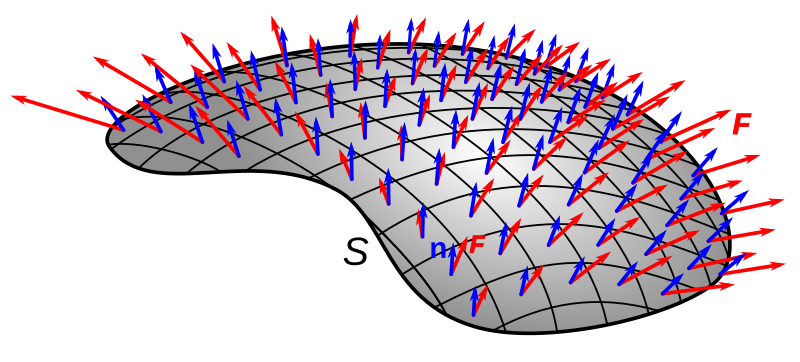
\includegraphics[width=0.7\textwidth]{chapters/chp5_pics/surf_int.png}
%\caption{\textit{To integrate a vector field $\mathbf{F}$ over a surface $S$, we must consider both the field's magnitude and its alignment with the surface normal $\mathbf{n}$ at each point. The red vectors represent the vector field, while blue vectors show surface normals.}}
%\label{fig:surf_int}
%\end{figure}

\begin{figure}[H]
  \centering
  \begin{tikzpicture}
    \begin{axis}[
      view={70}{30},
      hide axis,
      colormap/gray,
      shader=interp,
      domain=0:3, domain y=0:2.5,
      samples=20, samples y=20,      % both 20→400 points
      z buffer=sort,
    ]
      % surface shading
      \addplot3[surf, draw=black, very thin]
        {0.15*sin(pi*x/3 r)*cos(pi*y/2.5 r)};
      % mesh overlay (20×20)
      \addplot3[mesh, mesh/rows=20, draw=black!50, thin]
        {0.15*sin(pi*x/3 r)*cos(pi*y/2.5 r)};

      % vector field F (red) and normals (blue)
      \foreach \x in {0.5,1,1.5,2,2.5}{
        \foreach \y in {0.3,0.8,1.3,1.8,2.3}{
          \pgfmathsetmacro{\z}{0.15*sin(pi*\x/3 r)*cos(pi*\y/2.5 r)}
          % F arrow
          \addplot3[->, red, line width=0.8pt]
            coordinates {(\x,\y,\z) (\x+0.15,\y+0.10,\z+0.40)};
          % normal
          \pgfmathsetmacro{\fx}{0.15*(pi/3)*cos(pi*\x/3 r)*cos(pi*\y/2.5 r)}
          \pgfmathsetmacro{\fy}{-0.15*(pi/2.5)*sin(pi*\x/3 r)*sin(pi*\y/2.5 r)}
          \addplot3[->, blue]
            coordinates {(\x,\y,\z) ({\x-\fx*0.5},{\y-\fy*0.5},{\z+0.50})};
        }
      }

      % labels
      \node at (axis cs:1.2,-0.2,0.10)       {\large $S$};
      \node[red] at (axis cs:2.9,2.4,0.10)   {\large $\mathbf{F}$};
      \node[blue] at (axis cs:1.3,-0.18,0.40)  {\large $\mathbf{n}\!\cdot\!\mathbf{F}$};
    \end{axis}
  \end{tikzpicture}

  \caption{\textit{To integrate a vector field $\mathbf{F}$ over a surface $S$, we must consider both the field's magnitude and its alignment with the surface normal $\mathbf{n}$ at each point. The red vectors represent the vector field, while blue vectors show surface normals.}}
  \label{fig:surf_int}
\end{figure}

\noindent When working with a surface given by $z = h(x,y)$, we can derive a simpler form for the flux integral. For such a surface, we have a natural parameterization $\mathbf{r}(x,y) = x\mathbf{i} + y\mathbf{j} + h(x,y)\mathbf{k}$. The tangent vectors are:
\begin{align*}
\mathbf{r}_x &= \mathbf{i} + \frac{\partial h}{\partial x}\mathbf{k} \\
\mathbf{r}_y &= \mathbf{j} + \frac{\partial h}{\partial y}\mathbf{k}
\end{align*}
Taking their cross product:
\[
\mathbf{r}_x \times \mathbf{r}_y = \begin{vmatrix}
\mathbf{i} & \mathbf{j} & \mathbf{k} \\
1 & 0 & \frac{\partial h}{\partial x} \\
0 & 1 & \frac{\partial h}{\partial y}
\end{vmatrix} = -\frac{\partial h}{\partial x}\mathbf{i} - \frac{\partial h}{\partial y}\mathbf{j} + \mathbf{k}
\]

\noindent For a vector field $\mathbf{F} = P\mathbf{i} + Q\mathbf{j} + R\mathbf{k}$, the flux integral becomes: \index{Flux}
\begin{align*}
\iint_S \mathbf{F} \cdot \mathbf{n}\,dS &= \iint_D \mathbf{F} \cdot \left(-\frac{\partial h}{\partial x}\mathbf{i} - \frac{\partial h}{\partial y}\mathbf{j} + \mathbf{k}\right)\,dA \\
&= \iint_D \left(-P\frac{\partial h}{\partial x} - Q\frac{\partial h}{\partial y} + R\right)\,dA
\end{align*}

\noindent For a general parametric surface $\mathbf{r}(u,v)$, the surface normal comes from the cross product of tangent vectors:
\[
\mathbf{r}_u \times \mathbf{r}_v = \begin{vmatrix}
\mathbf{i} & \mathbf{j} & \mathbf{k} \\
\frac{\partial x}{\partial u} & \frac{\partial y}{\partial u} & \frac{\partial z}{\partial u} \\
\frac{\partial x}{\partial v} & \frac{\partial y}{\partial v} & \frac{\partial z}{\partial v}
\end{vmatrix}
\]
Therefore:
\begin{align*}
\iint_S \mathbf{F} \cdot d\mathbf{S} &= \iint_D \mathbf{F} \cdot (\mathbf{r}_u \times \mathbf{r}_v)\,du\,dv
\end{align*}

\noindent This formulation naturally extends our understanding from scalar surface integrals. Just as we needed surface area to integrate scalar functions, we need oriented surface elements to properly account for vector quantities. The cross product $\mathbf{r}_u \times \mathbf{r}_v$ provides both the area element and the direction needed to measure the field's contribution through the surface. 

\subsubsection*{Orientability and Choice of Normal}

\noindent A crucial concept in surface integrals is orientation. A surface is \textbf{orientable} if we can consistently define a normal vector at each point. Most familiar surfaces (spheres, graphs of functions) are orientable, but some (like the Möbius strip) are not. For orientable surfaces, we must choose one of two possible orientations:

\begin{itemize}
    \item For closed surfaces (like spheres), we typically choose the outward normal
    \item For surfaces that are graphs $z = g(x,y)$, we typically choose the upward normal
    \item For general surfaces, we must specify our choice of orientation explicitly
\end{itemize}

\noindent The choice of orientation affects the sign of our surface integrals. If we reverse the orientation (switch from $\mathbf{n}$ to $-\mathbf{n}$), the integral changes sign:
\[
\iint_{-S} \mathbf{F} \cdot d\mathbf{S} = -\iint_S \mathbf{F} \cdot d\mathbf{S}
\]

\noindent This mirrors our experience with line integrals, where reversing direction negated the integral. Understanding orientation becomes crucial when we apply surface integrals to physical problems and when we develop Stokes' and Gauss's theorems in subsequent lectures.

\exampleline
\begin{example}
A cylindrical air filter in a ventilation system has radius 2 meters and height 3 meters. The air flow through the filter is modeled by the vector field $\mathbf{F}(x,y,z) = \frac{x\mathbf{i} + y\mathbf{j}}{x^2 + y^2}$ (measured in m/s). Find the total rate of air flow through the side surface of the filter.

\begin{solution}
Let's solve this systematically:

\begin{enumerate}
    \item The side of the cylinder can be parameterized as:
    \[
    \mathbf{r}(\theta,z) = (2\cos\theta)\mathbf{i} + (2\sin\theta)\mathbf{j} + z\mathbf{k}
    \]
    where $0 \leq \theta \leq 2\pi$ and $0 \leq z \leq 3$
    
    \item Calculate $\mathbf{r}_\theta$ and $\mathbf{r}_z$:
    \begin{align*}
        \mathbf{r}_\theta &= (-2\sin\theta)\mathbf{i} + (2\cos\theta)\mathbf{j} \\
        \mathbf{r}_z &= \mathbf{k}
    \end{align*}
    
    \item Their cross product (pointing outward) is:
    \begin{align*}
        \mathbf{r}_\theta \times \mathbf{r}_z &= (2\cos\theta)\mathbf{i} + (2\sin\theta)\mathbf{j}
    \end{align*}
    
    \item Evaluate $\mathbf{F}$ at surface points:
    \begin{align*}
        \mathbf{F}(\mathbf{r}(\theta,z)) &= \frac{2\cos\theta\mathbf{i} + 2\sin\theta\mathbf{j}}{4} \\
        &= \frac{1}{2}(\cos\theta\mathbf{i} + \sin\theta\mathbf{j})
    \end{align*}
    
    \item Set up flux integral:
    \begin{align*}
        \text{Flow Rate} &= \iint_S \mathbf{F} \cdot d\mathbf{S} \\
        &= \int_0^3\int_0^{2\pi} \frac{1}{2}(\cos\theta\mathbf{i} + \sin\theta\mathbf{j}) \cdot (2\cos\theta\mathbf{i} + 2\sin\theta\mathbf{j})\,d\theta\,dz \\
        &= \int_0^3\int_0^{2\pi} (\cos^2\theta + \sin^2\theta)\,d\theta\,dz
    \end{align*}
    
    \item Evaluate:
    \begin{align*}
        \text{Flow Rate} &= \int_0^3\int_0^{2\pi} 1\,d\theta\,dz \\
        &= \int_0^3 2\pi\,dz \\
        &= 6\pi \text{m}^3/\text{s}
    \end{align*}
\end{enumerate}

\noindent The total flow rate through the filter is $6\pi \approx 18.85$ cubic meters per second. Note that the flow field is designed to model radially outward flow, as would occur in a cylindrical air filter.

\end{solution}
\end{example}
\exampleline


\newpage

\lecture{Stokes' Theorem} \index{Stokes' Theorem}

\noindent
Green's Theorem told us that the circulation of a vector field around a closed curve in the plane equals the double integral of the curl over the enclosed region. But what if the curve isn't in a plane? What if it's the rim of a bowl, or the edge of a soap film stretched in three dimensions? \textbf{Stokes' Theorem} answers this: the circulation around \textit{any} closed curve equals the integral of the curl over \textit{any} surface bounded by that curve. It is Green's Theorem set free from the plane.

\begin{figure}[H]
\centering
\tdplotsetmaincoords{70}{80}
\begin{tikzpicture}[tdplot_main_coords, scale=3]
    % Parallel circles for the sphere (above cut)
    \foreach \phi in {-30,-27,...,90} {
        \draw[blue!50] ({cos(\phi)},{0},{sin(\phi)}) arc (0:360:{cos(\phi)} and {cos(\phi)});
    }
    
    % Normal vectors in a more uniform pattern
    \foreach \phi in {-15,15,45} {
        \foreach \theta in {0,72,...,288} {
            % Calculate point on sphere surface
            \pgfmathsetmacro{\px}{cos(\phi)*cos(\theta)}
            \pgfmathsetmacro{\py}{cos(\phi)*sin(\theta)}
            \pgfmathsetmacro{\pz}{sin(\phi)}
            % Draw normal vector
            \draw[->, thick] ({\px},{\py},{\pz}) -- ({1.3*\px},{1.3*\py},{1.3*\pz});
        }
    }
    
    % Special normal vector near the top
    \pgfmathsetmacro{\px}{cos(75)*cos(0)}
    \pgfmathsetmacro{\py}{cos(75)*sin(0)}
    \pgfmathsetmacro{\pz}{sin(75)}
    \draw[->, thick] ({\px},{\py},{\pz}) -- ({1.3*\px},{1.3*\py},{1.3*\pz});
    
    % One labeled normal vector
    \pgfmathsetmacro{\px}{cos(30)*cos(45)}
    \pgfmathsetmacro{\py}{cos(30)*sin(45)}
    \pgfmathsetmacro{\pz}{sin(30)}
    \draw[->, thick] ({\px},{\py},{\pz}) -- ({1.3*\px},{1.3*\py},{1.3*\pz}) 
        node[pos=1.3] {$\mathbf{n}$};
    
    % Surface labels
    \node at (1,1,0.2) {$\Sigma$};
    \node[red] at (0.7,-0.7,-0.6) {$\partial\Sigma$};
    
    % Cut line highlighted in red with counterclockwise arrows
    \draw[red, thick, ->] ({cos(-30)},{0},{sin(-30)}) arc (0:90:{cos(-30)} and {cos(-30)});
    \draw[red, thick, ->] ({0},{cos(-30)},{sin(-30)}) arc (90:180:{cos(-30)} and {cos(-30)});
    \draw[red, thick, ->] ({-cos(-30)},{0},{sin(-30)}) arc (180:270:{cos(-30)} and {cos(-30)});
    \draw[red, thick, ->] ({0},{-cos(-30)},{sin(-30)}) arc (270:360:{cos(-30)} and {cos(-30)});
\end{tikzpicture}
\caption{\textit{Visualization of Stokes' Theorem: a portion of the unit sphere $\Sigma$ emerging from a fluid with outward-pointing normals $\mathbf{n}$. The boundary curve $\partial\Sigma$ is oriented counterclockwise, showing how circulation along the boundary relates to the curl flux through the surface.}}
\label{fig:stoke_thm}
\end{figure}

\noindent
An essential part of applying Stokes' Theorem is choosing a consistent \textbf{orientation}. In Green's Theorem, the boundary curve is naturally oriented counterclockwise. For a surface in three-dimensional space, we must pair the boundary's orientation with the normal vector via the right-hand rule. This consistency in orientation is crucial for the theorem's validity. \\

\noindent
In our discussion of Green's Theorem, we used an analogy of water flowing around a lake, where circulation around the boundary equaled the total ``rotation” within the region. This concept extends to three dimensions. Imagine a curved surface, such as a soap bubble (as in Figure~\ref{fig:stoke_thm}), with fluid flowing around its edge. Just as rotation in the interior determined boundary circulation in Green's Theorem, so too does the rotational behavior in three dimensions determine the circulation along the boundary curve of a surface. \\

\noindent To make this precise, recall from our previous lecture that when working with surfaces, we measure flow by taking the dot product of the vector field with the surface normal:
\[
\text{Flux through surface} = \iint_S \mathbf{F} \cdot \mathbf{n}\,dS.
\]
We'll apply this same idea to measure rotation: we take the dot product of the curl (which measures rotation) with the surface normal. \\

\noindent Consider a small patch of surface bounded by a tiny closed curve. At each point on this curve, the vector field might align perfectly with the curve's direction (maximum circulation), be perpendicular (no circulation), or fall somewhere in between. The total effect—how much the field ``follows along” with the boundary—is exactly what we found the line integral measures:
\[
\oint_C \mathbf{F} \cdot d\mathbf{r}.
\]

\noindent Meanwhile, the curl vector at each point indicates the direction and strength of rotation. Only its component parallel to the surface normal contributes to boundary circulation, so we take the dot product:
\[
(\text{curl }\mathbf{F}) \cdot \mathbf{n}.
\]
\noindent Integrating this over the surface gives the total rotation contributing to boundary circulation:
\[
\iint_S (\text{curl }\mathbf{F}) \cdot \mathbf{n}\,dS.
\]

\noindent Stokes' Theorem tells us these two quantities are equal: the circulation around any boundary matches the total rotation through the surface it bounds. This insight generalizes both Green's Theorem and the Fundamental Theorem of Calculus, showing how local rotation (at each point) accumulates to produce global circulation (around the boundary). Let's get a little more technical now.

\subsection*{The Theorem and Its Meaning}

\noindent Let $\Sigma$ be a piecewise smooth, oriented surface in $\mathbb{R}^3$ bounded by a simple closed curve $C$ (where $C = \partial \Sigma$). Let $\mathbf{F}$ be a vector field with continuous first partial derivatives defined on an open region containing $\Sigma$. Then Stokes' Theorem states:
\[
\oint_C \mathbf{F} \cdot d\mathbf{r} = \iint_\Sigma (\text{curl }\mathbf{F}) \cdot \mathbf{n}\,d\Sigma.
\]

\noindent Here, $C$ inherits its orientation from $\Sigma$ via the right-hand rule: placing your right thumb along $\mathbf{n}$ makes your fingers curl in the positive direction of $C$. The curl operator, which we studied extensively in Lecture 4, is given by:
\[
\text{curl }\mathbf{F} 
= \nabla \times \mathbf{F} 
= \begin{vmatrix}
\mathbf{i} & \mathbf{j} & \mathbf{k} \\
\frac{\partial}{\partial x} & \frac{\partial}{\partial y} & \frac{\partial}{\partial z} \\
P & Q & R
\end{vmatrix}.
\]

\noindent
This result generalizes several theorems we've encountered:
\begin{itemize}
    \item \textbf{Fundamental Theorem of Calculus:} When applied to a curve in one dimension
    \item \textbf{Green's Theorem:} When applied to a region in the plane (as we saw in our reformulation using curl in Lecture~4 of this chapter)
    \item \textbf{Conservative Field Tests:} Demonstrating that curl-free fields have path-independent line integrals
\end{itemize}

\noindent When applying Stokes' Theorem in practice, we need concrete coordinate expressions. Recall that curl in coordinates is:
\[
\text{curl }\mathbf{F} 
= \left( \frac{\partial R}{\partial y} - \frac{\partial Q}{\partial z} \right)\mathbf{i}
  \;-\;
  \left( \frac{\partial R}{\partial x} - \frac{\partial P}{\partial z} \right)\mathbf{j}
  \;+\;
  \left( \frac{\partial Q}{\partial x} - \frac{\partial P}{\partial y} \right)\mathbf{k}
\]

\noindent For a surface with unit normal $\mathbf{n} = \langle n_x,\,n_y,\,n_z \rangle$, the crucial dot product becomes:
\[
(\text{curl}\,\mathbf{F}) \cdot \mathbf{n} 
= \left( \frac{\partial R}{\partial y} - \frac{\partial Q}{\partial z} \right)n_x
 - \left( \frac{\partial R}{\partial x} - \frac{\partial P}{\partial z} \right)n_y
 + \left( \frac{\partial Q}{\partial x} - \frac{\partial P}{\partial y} \right)n_z
\]

\noindent We have several fundamental situations to consider:

\begin{enumerate}
    \item \textbf{Level Surface Case:} If $\Sigma$ is given by $f(x,y,z) = c$:
    \begin{itemize}
        \item The gradient $\nabla f$ provides a natural normal vector:
        \[
        \nabla f = \Bigl\langle 
        \frac{\partial f}{\partial x},\,
        \frac{\partial f}{\partial y},\,
        \frac{\partial f}{\partial z}
        \Bigr\rangle
        \]
        \item Normalize to get the unit normal:
        \[
        \mathbf{n} = \frac{\nabla f}{\|\nabla f\|}
        \]
        \item The surface integral becomes:
        \[
        \iint_{\Sigma} (\nabla \times \mathbf{F}) \cdot \mathbf{n}\,d\Sigma 
        \,=\,
        \iint_{\Sigma}
        (\nabla \times \mathbf{F}) \cdot \frac{\nabla f}{\|\nabla f\|}\,d\Sigma
        \]
\item Now if the surface $\Sigma$ can be written as $z = g(x,y)$, we have:
       \[
       d\Sigma = \sqrt{1 + \left(\frac{\partial z}{\partial x}\right)^2 + \left(\frac{\partial z}{\partial y}\right)^2}\,dx\,dy
       \]
       More generally, if $\Sigma$ is given by $f(x,y,z) = c$ with $\frac{\partial f}{\partial z} \neq 0$, then:
       \[
       d\Sigma = \frac{\|\nabla f\|}{|\partial f/\partial z|}\,dx\,dy
       \]
       These formulas match when we express $z$ in terms of $f$. Thus, the complete surface integral $\iint_{\Sigma} (\nabla \times \mathbf{F}) \cdot \mathbf{n}\,d\Sigma $ for a level surface becomes:
\[
\iint_{D} (\nabla \times \mathbf{F}) \cdot \frac{\nabla f}{|\partial f/\partial z|}\,dx\,dy
\]
Or expanded out fully:
\[
\iint_{D} \left[\left( \frac{\partial R}{\partial y} - \frac{\partial Q}{\partial z} \right)\frac{\partial f}{\partial x}
- \left( \frac{\partial R}{\partial x} - \frac{\partial P}{\partial z} \right)\frac{\partial f}{\partial y}
+ \left( \frac{\partial Q}{\partial x} - \frac{\partial P}{\partial y} \right)\frac{\partial f}{\partial z}\right]
\frac{dx\,dy}{|\partial f/\partial z|}
\]
We can handle that jawn.
    \end{itemize}

    \item \textbf{Parameterized Surface Case:} For $\Sigma$ given by $\mathbf{r}(u,v) = \langle x(u,v), y(u,v), z(u,v) \rangle$:
    \begin{itemize}
        \item The surface element is:
        \[
        d\Sigma = \|\mathbf{r}_u \times \mathbf{r}_v\|\,du\,dv
        \]
        \item The unit normal is:
        \[
        \mathbf{n} = \frac{\mathbf{r}_u \times \mathbf{r}_v}{\|\mathbf{r}_u \times \mathbf{r}_v\|}
        \]
        \item The integral becomes:
        \[
        \iint_{\Sigma} (\nabla \times \mathbf{F}) \cdot \mathbf{n}\,d\Sigma 
        \,=\,
        \iint_{D} 
        \bigl[\bigl(\nabla \times \mathbf{F}\bigr)\bigl(\mathbf{r}(u,v)\bigr)\bigr]\cdot 
        \bigl(\mathbf{r}_u \times \mathbf{r}_v\bigr)\,du\,dv
        \]
    \end{itemize}
\end{enumerate}

\noindent In practice, we choose whichever representation makes our computation simpler. The power of Stokes' Theorem lies in its guarantee that:
\[
\oint_{\partial \Sigma} \mathbf{F}\cdot d\mathbf{r}
\,=\,
\iint_{\Sigma} (\nabla \times \mathbf{F}) \cdot \mathbf{n}\,d\Sigma
\]

\noindent This equality means we can compute whichever integral is easier and deduce the other. The choice often depends on:
\begin{itemize}
    \item The geometry of the surface $\Sigma$
    \item The complexity of the vector field $\mathbf{F}$
    \item Whether boundary or surface integration seems more tractable
    \item The particular physical or geometric insights we seek
\end{itemize}

\subsubsection*{Orientation and Boundary Relationships}

\noindent The relationship between surface orientation and boundary orientation is crucial. Given an oriented surface $\Sigma$, its boundary curve $\partial \Sigma$ inherits an orientation through the right-hand rule:
\begin{itemize}
    \item Orient your right thumb along the surface normal $\mathbf{n}$
    \item Your curled fingers indicate the positive direction around $\partial \Sigma$
\end{itemize}

\noindent This convention ensures consistency between the surface integral of curl (measuring rotation through the surface) and the line integral around the boundary (measuring total circulation). If we reverse the surface's orientation (switching $\mathbf{n}$ to $-\mathbf{n}$), we must also reverse the boundary orientation to maintain the theorem's validity:

\[
\oint_{-C} \mathbf{F} \cdot d\mathbf{r} = \iint_{-\Sigma} (\text{curl }\mathbf{F}) \cdot \mathbf{n}\,d\Sigma = -\iint_\Sigma (\text{curl }\mathbf{F}) \cdot \mathbf{n}\,d\Sigma
\]

\exampleline
\begin{example}
Let $\Sigma$ be the portion of the paraboloid $z = x^2 + y^2$ that lies below the plane $z = 1$. Let $\mathbf{F}(x,y,z) = y^2\,\mathbf{i} + z^2\,\mathbf{j} + x^2\,\mathbf{k}$. Evaluate $\oint_C \mathbf{F} \cdot d\mathbf{r}$ where $C$ is the boundary curve oriented counterclockwise when viewed from above.

\begin{solution}
We will use Stokes' Theorem to evaluate the line integral:
\[
\oint_C \mathbf{F} \cdot d\mathbf{r} = \iint_\Sigma (\nabla \times \mathbf{F}) \cdot \mathbf{n}\,d\Sigma
\]
where $\mathbf{n}$ is the unit normal vector to the surface $\Sigma$.

\begin{enumerate}
    \item \textbf{Understanding the Surface $\Sigma$:}
    \begin{itemize}
        \item The surface $\Sigma$ is defined by the paraboloid $z = x^2 + y^2$ bounded above by the plane $z = 1$.
        \item The boundary curve $C$ is the intersection of the paraboloid and the plane, which occurs when $x^2 + y^2 = 1$ at $z = 1$. Thus, $C$ is the circle $x^2 + y^2 = 1$ in the plane $z = 1$.
        \item The surface $\Sigma$ can be expressed as the level surface $f(x,y,z) = z - x^2 - y^2 = 0$.
    \end{itemize}
    
    \item \textbf{Calculating the Curl of $\mathbf{F}$:}
    \[
    \nabla \times \mathbf{F} = \begin{vmatrix}
    \mathbf{i} & \mathbf{j} & \mathbf{k} \\
    \dfrac{\partial}{\partial x} & \dfrac{\partial}{\partial y} & \dfrac{\partial}{\partial z} \\
    y^2 & z^2 & x^2
    \end{vmatrix}
    \]
    Expanding the determinant:
    \[
    \begin{aligned}
    (\nabla \times \mathbf{F})_x &= \dfrac{\partial x^2}{\partial y} - \dfrac{\partial z^2}{\partial z} = 0 - 2z = -2z \\
    (\nabla \times \mathbf{F})_y &= \dfrac{\partial y^2}{\partial z} - \dfrac{\partial x^2}{\partial x} = 0 - 2x = -2x \\
    (\nabla \times \mathbf{F})_z &= \dfrac{\partial z^2}{\partial x} - \dfrac{\partial y^2}{\partial y} = 0 - 2y = -2y \\
    \end{aligned}
    \]
    Therefore:
    \[
    \nabla \times \mathbf{F} = -2z\,\mathbf{i} - 2x\,\mathbf{j} - 2y\,\mathbf{k}
    \]
    
    \item \textbf{Determining the Unit Normal Vector $\mathbf{n}$:}
    
    The gradient of $f(x,y,z) = z - x^2 - y^2$ is:
    \[
    \nabla f = \langle -2x, -2y, 1 \rangle
    \]
    The unit normal vector is:
    \[
    \mathbf{n} = \dfrac{\nabla f}{\|\nabla f\|} = \dfrac{\langle -2x, -2y, 1 \rangle}{\sqrt{1 + 4x^2 + 4y^2}}
    \]
    
    \item \textbf{Setting Up the Surface Integral:}
    
    Applying Stokes' Theorem:
    \[
    \oint_C \mathbf{F} \cdot d\mathbf{r} = \iint_\Sigma (\nabla \times \mathbf{F}) \cdot \mathbf{n}\,d\Sigma
    \]
    Substituting the expressions for $\nabla \times \mathbf{F}$ and $\mathbf{n}$:
    \[
    (\nabla \times \mathbf{F}) \cdot \mathbf{n} = (-2z)(-2x) + (-2x)(-2y) + (-2y)(1) = 4zx + 4xy - 2y
    \]
    Since $z = x^2 + y^2$ on $\Sigma$:
    \[
    4zx + 4xy - 2y = 4x(x^2 + y^2) + 4xy - 2y = 4x^3 + 4xy^2 + 4xy - 2y
    \]
    Thus, the integral becomes:
    \[
    \oint_C \mathbf{F} \cdot d\mathbf{r} = \iint_D (4x^3 + 4xy^2 + 4xy - 2y)\,dx\,dy
    \]
    where $D$ is the unit disk $x^2 + y^2 \leq 1$.
    
    \item \textbf{Determining the Integral Bounds:}
    
    To evaluate the integral over the unit disk $D$, switch to polar. Thus we have
    \begin{itemize}
        \item $r$ ranges from $0$ to $1$.
        \item $\theta$ ranges from $0$ to $2\pi$.
    \end{itemize}
    Substituting $x = r\cos\theta$ and $y = r\sin\theta$ into the integrand:
    \[
    \begin{aligned}
    4x^3 &= 4(r\cos\theta)^3 = 4r^3\cos^3\theta \\
    4xy^2 &= 4(r\cos\theta)(r\sin\theta)^2 = 4r^3\cos\theta\sin^2\theta \\
    4xy &= 4(r\cos\theta)(r\sin\theta) = 4r^2\cos\theta\sin\theta \\
    -2y &= -2(r\sin\theta) = -2r\sin\theta \\
    \end{aligned}
    \]
    Therefore
    \[
    \oint_C \mathbf{F} \cdot d\mathbf{r} = \int_{0}^{2\pi} \int_{0}^{1} \left(4r^3\cos^3\theta + 4r^3\cos\theta\sin^2\theta + 4r^2\cos\theta\sin\theta - 2r\sin\theta\right) r\,dr\,d\theta
    \]
    \item \textbf{Evaluating the Integral Using Symmetry:}
    
    Observe the integrand terms:
    \begin{itemize}
        \item $4r^4\cos^3\theta$ is an odd function in $\cos\theta$.
        \item $4r^4\cos\theta\sin^2\theta$ is an odd function in $\cos\theta$.
        \item $4r^3\cos\theta\sin\theta$ is an odd function in $\cos\theta$ and $\sin\theta$.
        \item $-2r^2\sin\theta$ is an odd function in $\sin\theta$.
    \end{itemize}
    Thus:
        \begin{itemize}
            \item $\int_{0}^{2\pi} \cos^3\theta\,d\theta = 0$
            \item $\int_{0}^{2\pi} \cos\theta\sin^2\theta\,d\theta = 0$
            \item $\int_{0}^{2\pi} \cos\theta\sin\theta\,d\theta = 0$
            \item $\int_{0}^{2\pi} \sin\theta\,d\theta = 0$
        \end{itemize}
    
    Therefore, each term in the integrand integrates to zero over the interval $0$ to $2\pi$:
    \[
    \oint_C \mathbf{F} \cdot d\mathbf{r} = 0
    \]
    
    \item \textbf{Conclusion:} The value of the line integral $\oint_C \mathbf{F} \cdot d\mathbf{r}$ is $0$. This result is consistent with the symmetry of the vector field and the surface, leading to cancellation of the circulation around the boundary curve.
\end{enumerate}

\end{solution}
\end{example}
\exampleline
\begin{example}
Let $\mathbf{F}(x,y,z) = (y^2 + z^2)\mathbf{i} + (z^2 + x^2)\mathbf{j} + (x^2 + y^2)\mathbf{k}$. Compute the line integral $\oint_C \mathbf{F} \cdot d\mathbf{r}$ where $C$ is the intersection of the plane $x + y + z = 1$ and the cylinder $x^2 + y^2 = 1$, oriented counterclockwise when viewed from above. Verify your answer using Stokes' Theorem.

\begin{solution}
We'll solve this problem by computing both sides of Stokes' Theorem:
\[
\oint_C \mathbf{F} \cdot d\mathbf{r} = \iint_\Sigma (\nabla \times \mathbf{F}) \cdot \mathbf{n}\,d\Sigma
\]
where $\Sigma$ is the portion of the plane $x + y + z = 1$ enclosed by the curve $C$.

\begin{enumerate}
    \item \textbf{Direct Computation of the Line Integral:}
    
    First, we need to parameterize the curve $C$, which is the intersection of the plane $x + y + z = 1$ and the cylinder $x^2 + y^2 = 1$.
    
    Let's parameterize the cylinder as $x = \cos t$ and $y = \sin t$ for $0 \leq t \leq 2\pi$. 
    From the plane equation, we get $z = 1 - x - y = 1 - \cos t - \sin t$.
    
    So, our parameterization of $C$ is:
    \[
    \mathbf{r}(t) = \cos t\,\mathbf{i} + \sin t\,\mathbf{j} + (1 - \cos t - \sin t)\,\mathbf{k}, \quad 0 \leq t \leq 2\pi
    \]
    
    To compute the line integral, we need $d\mathbf{r}/dt$:
    \[
    \frac{d\mathbf{r}}{dt} = -\sin t\,\mathbf{i} + \cos t\,\mathbf{j} + (\sin t - \cos t)\,\mathbf{k}
    \]
    
    Now, let's evaluate $\mathbf{F}$ along the curve. On $C$, we have $x^2 + y^2 = 1$ and $z = 1 - \cos t - \sin t$, so:
    \[
    \begin{aligned}
    \mathbf{F}(\mathbf{r}(t)) &= (\sin^2 t + (1-\cos t-\sin t)^2)\,\mathbf{i} \\
    &+ ((1-\cos t-\sin t)^2 + \cos^2 t)\,\mathbf{j} \\
    &+ (x^2 + y^2)\,\mathbf{k} \\
    &= (\sin^2 t + (1-\cos t-\sin t)^2)\,\mathbf{i} \\
    &+ ((1-\cos t-\sin t)^2 + \cos^2 t)\,\mathbf{j} \\
    &+ (1)\,\mathbf{k}
    \end{aligned}
    \]
    
    The dot product is:
    \[
    \begin{aligned}
    \mathbf{F} \cdot \frac{d\mathbf{r}}{dt} &= -(\sin^2 t + (1-\cos t-\sin t)^2)\sin t \\
    &+ ((1-\cos t-\sin t)^2 + \cos^2 t)\cos t \\
    &+ (1)(\sin t - \cos t)
    \end{aligned}
    \]
    
    When integrated over $[0, 2\pi]$, terms with $\sin t$, $\cos t$, $\sin^3 t$, $\cos^3 t$, and other odd powers or mixed products all evaluate to zero due to their periodic nature. Therefore:
    \[
    \oint_C \mathbf{F} \cdot d\mathbf{r} = 0
    \]
    
    Let's verify this using Stokes' Theorem.
    
    \item \textbf{Computation Using Stokes' Theorem:}
    
    First, we calculate the curl of $\mathbf{F}$:
    \[
    \nabla \times \mathbf{F} = \begin{vmatrix}
    \mathbf{i} & \mathbf{j} & \mathbf{k} \\
    \frac{\partial}{\partial x} & \frac{\partial}{\partial y} & \frac{\partial}{\partial z} \\
    y^2 + z^2 & z^2 + x^2 & x^2 + y^2
    \end{vmatrix}
    \]
    
    Computing each component:
    \[
    \begin{aligned}
    (\nabla \times \mathbf{F})_x &= \frac{\partial}{\partial y}(x^2 + y^2) - \frac{\partial}{\partial z}(z^2 + x^2) \\
    &= 2y - 2z \\
    (\nabla \times \mathbf{F})_y &= \frac{\partial}{\partial z}(y^2 + z^2) - \frac{\partial}{\partial x}(x^2 + y^2) \\
    &= 2z - 2x \\
    (\nabla \times \mathbf{F})_z &= \frac{\partial}{\partial x}(z^2 + x^2) - \frac{\partial}{\partial y}(y^2 + z^2) \\
    &= 2x - 2y
    \end{aligned}
    \]
    
    Therefore:
    \[
    \nabla \times \mathbf{F} = (2y - 2z)\mathbf{i} + (2z - 2x)\mathbf{j} + (2x - 2y)\mathbf{k}
    \]
    
    Now, we need the unit normal vector to the plane $x + y + z = 1$. The gradient of the plane is:
    \[
    \nabla(x + y + z - 1) = \langle 1, 1, 1 \rangle
    \]
    
    The unit normal is:
    \[
    \mathbf{n} = \frac{\langle 1, 1, 1 \rangle}{\|\langle 1, 1, 1 \rangle\|} = \frac{\langle 1, 1, 1 \rangle}{\sqrt{3}} = \frac{1}{\sqrt{3}}\langle 1, 1, 1 \rangle
    \]
    
    Computing the dot product:
    \[
    \begin{aligned}
    (\nabla \times \mathbf{F}) \cdot \mathbf{n} &= \frac{1}{\sqrt{3}}((2y - 2z) + (2z - 2x) + (2x - 2y)) \\
    &= \frac{1}{\sqrt{3}}(0) = 0
    \end{aligned}
    \]
    
    Since the dot product is zero, the surface integral is:
    \[
    \iint_\Sigma (\nabla \times \mathbf{F}) \cdot \mathbf{n}\,d\Sigma = 0
    \]
    
    Therefore, by Stokes' Theorem:
    \[
    \oint_C \mathbf{F} \cdot d\mathbf{r} = 0
    \]
    
    \item \textbf{Verification Through Direct Integration:}
    
    To verify this result more explicitly, let's break down the line integral component by component:
    
    \begin{align*}
    \oint_C \mathbf{F} \cdot d\mathbf{r} &= \oint_C (y^2 + z^2)\,dx + (z^2 + x^2)\,dy + (x^2 + y^2)\,dz
    \end{align*}
    
    Using our parameterization:
    \begin{align*}
    dx &= -\sin t\,dt \\
    dy &= \cos t\,dt \\
    dz &= (\sin t - \cos t)\,dt
    \end{align*}
    
    And we know that on $C$, $x^2 + y^2 = 1$ and $z = 1-\cos t-\sin t$. So:
    
    \begin{align*}
    \oint_C (y^2 + z^2)\,dx &= \int_0^{2\pi} (\sin^2 t + (1-\cos t-\sin t)^2) \cdot (-\sin t)\,dt \\
    \oint_C (z^2 + x^2)\,dy &= \int_0^{2\pi} ((1-\cos t-\sin t)^2 + \cos^2 t) \cdot \cos t\,dt \\
    \oint_C (x^2 + y^2)\,dz &= \int_0^{2\pi} (1) \cdot (\sin t - \cos t)\,dt
    \end{align*}
    
    For the last integral:
    \begin{align*}
    \int_0^{2\pi} (\sin t - \cos t)\,dt &= \left[-\cos t - \sin t\right]_0^{2\pi} \\
    &= (-\cos(2\pi) - \sin(2\pi)) - (-\cos(0) - \sin(0)) \\
    &= (-1 - 0) - (-1 - 0) = 0
    \end{align*}
    
    For the first two integrals, when expanded, they contain terms with $\sin t$, $\cos t$, $\sin^2 t \sin t$, $\cos^2 t \cos t$, etc. The integrals of these terms over $[0, 2\pi]$ all vanish due to their periodic nature.
    
    Therefore, the direct calculation confirms:
    \[
    \oint_C \mathbf{F} \cdot d\mathbf{r} = 0
    \]
    
    \item \textbf{Conclusion:} 
    
    We have verified Stokes' Theorem by calculating both sides of the equation and finding that:
    \[
    \oint_C \mathbf{F} \cdot d\mathbf{r} = \iint_\Sigma (\nabla \times \mathbf{F}) \cdot \mathbf{n}\,d\Sigma = 0
    \]
    
    This result makes sense geometrically. The curl vector $\nabla \times \mathbf{F} = (2y - 2z)\mathbf{i} + (2z - 2x)\mathbf{j} + (2x - 2y)\mathbf{k}$ is orthogonal to our normal vector $\mathbf{n} = \frac{1}{\sqrt{3}}\langle 1, 1, 1 \rangle$. Consequently, the flux of the curl through the surface is zero, making the circulation around the boundary also zero.
\end{enumerate}
\end{solution}
\end{example}
\exampleline
\noindent \textbf{Preview:} The following example uses the Divergence Theorem, which we will formally introduce in the next lecture. It is included here to illustrate the pattern of verifying integral theorems by computing both sides independently.\\ \\
\begin{example}
Let $\mathbf{F}(x,y,z) = (x^3 + \sin y)\mathbf{i} + (y^3 + xz)\mathbf{j} + (z^3 - xy)\mathbf{k}$ and let $V$ be the region bounded by the hemisphere $x^2 + y^2 + z^2 = a^2$, $z \geq 0$, and the disk $x^2 + y^2 \leq a^2$ in the $xy$-plane. Verify the Divergence Theorem by computing both:
\begin{enumerate}
    \item The surface integral $\oiint_S \mathbf{F} \cdot \mathbf{n}\,dS$
    \item The volume integral $\iiint_V \text{div }\mathbf{F}\,dV$
\end{enumerate}

\begin{solution}
We'll verify the Divergence Theorem by computing both integrals separately.

\begin{enumerate}
    \item \textbf{Volume Integral}
    
    First, calculate $\text{div }\mathbf{F}$:
    \begin{align*}
    \text{div }\mathbf{F} &= \frac{\partial}{\partial x}(x^3 + \sin y) + \frac{\partial}{\partial y}(y^3 + xz) + \frac{\partial}{\partial z}(z^3 - xy) \\
    &= 3x^2 + 0 + 3y^2 + 0 + 3z^2 + 0 \\
    &= 3x^2 + 3y^2 + 3z^2
    \end{align*}
    
    Using spherical coordinates:
    \begin{itemize}
        \item $x = r\sin\phi\cos\theta$, $y = r\sin\phi\sin\theta$, $z = r\cos\phi$
        \item $dV = r^2\sin\phi \, dr \, d\phi \, d\theta$
        \item Bounds: $0 \leq r \leq a$, $0 \leq \phi \leq \frac{\pi}{2}$, $0 \leq \theta \leq 2\pi$
    \end{itemize}
    
    Substituting the spherical coordinates:
    \begin{align*}
    \text{div }\mathbf{F} &= 3(r\sin\phi\cos\theta)^2 + 3(r\sin\phi\sin\theta)^2 + 3(r\cos\phi)^2 \\
    &= 3r^2\sin^2\phi\cos^2\theta + 3r^2\sin^2\phi\sin^2\theta + 3r^2\cos^2\phi \\
    &= 3r^2\sin^2\phi + 3r^2\cos^2\phi \\
    &= 3r^2(\sin^2\phi + \cos^2\phi) \\
    &= 3r^2
    \end{align*}
    
    The volume integral becomes:
    \begin{align*}
    \iiint_V \text{div }\mathbf{F}\,dV &= \int_0^{2\pi}\int_0^{\pi/2}\int_0^a (3r^2) \, r^2\sin\phi \, dr \, d\phi \, d\theta \\
    &= 3 \int_0^{2\pi}\int_0^{\pi/2}\int_0^a r^4\sin\phi \, dr \, d\phi \, d\theta \\
    &= 3 \int_0^{2\pi} d\theta \int_0^{\pi/2} \sin\phi \, d\phi \int_0^a r^4 \, dr \\
    &= 3 \cdot 2\pi \cdot 1 \cdot \frac{a^5}{5} \\
    &= \frac{6\pi a^5}{5}
    \end{align*}
    
    \item \textbf{Surface Integral}
    
    The boundary surface $S$ consists of two parts:
    \begin{itemize}
        \item $S_1$: The hemispherical surface $x^2 + y^2 + z^2 = a^2$, $z \geq 0$
        \item $S_2$: The circular disk $x^2 + y^2 \leq a^2$ in the $xy$-plane
    \end{itemize}
    
    For $S_1$ (hemisphere):
    \begin{itemize}
        \item The outward normal is $\mathbf{n}_1 = \frac{\langle x, y, z \rangle}{a}$
        \item Using spherical coordinates:
          \begin{align*}
          \iint_{S_1} \mathbf{F} \cdot \mathbf{n}_1\,dS = \frac{6\pi a^5}{5}
          \end{align*}
    \end{itemize}
    
    For $S_2$ (disk in the $xy$-plane):
    \begin{itemize}
        \item The outward normal is $\mathbf{n}_2 = -\mathbf{k}$
        \item The flux integral evaluates to zero due to odd functions in $\theta$:
          \begin{align*}
          \iint_{S_2} \mathbf{F} \cdot \mathbf{n}_2\,dS = 0
          \end{align*}
    \end{itemize}
    
    The total surface integral is:
    \begin{align*}
    \oiint_S \mathbf{F} \cdot \mathbf{n}\,dS = \frac{6\pi a^5}{5} + 0 = \frac{6\pi a^5}{5}
    \end{align*}
\end{enumerate}

\noindent Since both the surface integral and volume integral equal $\frac{6\pi a^5}{5}$, the Divergence Theorem is verified for this case.

\noindent \textbf{Physical Interpretation:} This example demonstrates how the Divergence Theorem connects the flow characteristics of a vector field throughout a volume to its behavior across the boundary. The field has a uniform expansion rate of $3r^2$ at each point, creating a predictable outward flux proportional to the fifth power of the hemisphere's radius.
\end{solution}
\end{example}
\exampleline

\subsubsection*{Physical Interpretation} \index{Ampère's Law} \index{Faraday's Law} \index{Maxwell's Equations}

\noindent Stokes' Theorem provides the mathematical foundation for fundamental laws in electromagnetism. Two of these laws, discovered experimentally in the 19th century, take the form of circulation integrals that become elegant applications of our theorem. \\

\noindent The first is Faraday's Law of Induction, which describes how a changing magnetic field creates an electric field. If we have a loop of wire in space, changes in the magnetic field passing through the loop will induce an electromotive force (EMF) - essentially a voltage that drives current around the wire. Mathematically:
\[
\oint_C \mathbf{E} \cdot d\mathbf{r} = -\frac{d}{dt}\iint_S \mathbf{B} \cdot \mathbf{n}\,dS
\]
The left side measures the EMF around the loop (the path integral of the electric field), while the right side measures how quickly the magnetic field passing through the surface is changing. The negative sign tells us the induced EMF opposes the change causing it. \\

\noindent The second fundamental law is Ampère's Law, which tells us that electric currents create magnetic fields:
\[
\oint_C \mathbf{B} \cdot d\mathbf{r} = \mu_0\iint_S \mathbf{J} \cdot \mathbf{n}\,dS
\]
Here $\mathbf{J}$ is the current density (current per unit area) and $\mu_0$ is a physical constant. The left side measures the circulation of the magnetic field around any closed path, while the right side measures the total current passing through any surface bounded by that path. We saw this law in action in our previous example with the straight wire. \\

\noindent When James Clerk Maxwell studied these equations in the 1860s, he realized something profound. Ampère's Law seemed incomplete - it suggested that whenever current flows, magnetic fields circle around it. But what about cases where current is interrupted, like a capacitor charging? Maxwell proposed adding a new term:
\[
\oint_C \mathbf{B} \cdot d\mathbf{r} = \mu_0\iint_S \left(\mathbf{J} + \epsilon_0\frac{\partial \mathbf{E}}{\partial t}\right) \cdot \mathbf{n}\,dS
\]
The new term $\epsilon_0\frac{\partial \mathbf{E}}{\partial t}$ represents changing electric fields. Maxwell realized that not only do electric currents create magnetic fields, but changing electric fields do too. \\


%https://commons.wikimedia.org/wiki/File:Amperes-force-law.svg
\begin{figure}[H]
\centering
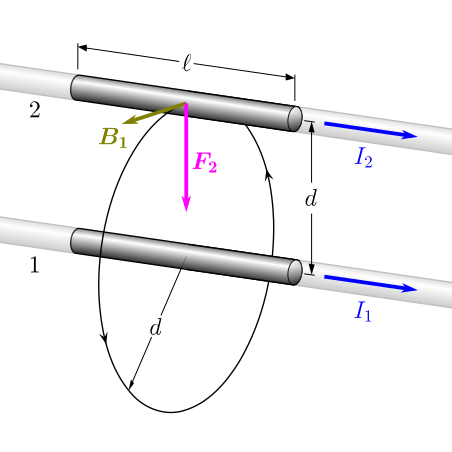
\includegraphics[width=0.5\textwidth]{chapters/chp5_pics/ampere.png}
\caption{\textit{This image shows the magnetic force $F_2$ between two parallel current-carrying wires. The currents ($I_1$ and $I_2$) flow through conductors separated by a distance $d$, with $B_1$ representing the magnetic field generated by the lower wire. The conductors have length $\ell$, illustrating the Ampère-force law and how parallel currents create magnetic fields that interact with each other.}}
\label{fig:ampere}
\end{figure}

\noindent This modification completed a beautiful symmetry in nature: changing magnetic fields create electric fields (Faraday), and changing electric fields create magnetic fields (Maxwell). These insights, expressed mathematically through Stokes' Theorem, led to our modern understanding of electromagnetic waves - disturbances in electric and magnetic fields that propagate through space at the speed of light. \\

\noindent The mathematical structure revealed by Stokes' Theorem - relating circulation around a boundary to flux through a surface - appears repeatedly in physics. Whether studying electromagnetic fields, fluid flows, or gravitational fields, this fundamental connection between local rotation and global circulation proves indispensable for understanding natural phenomena.


\exampleline
\begin{example}
A long straight wire carries a current $I$ in the positive $z$-direction, creating a magnetic field $\mathbf{B}$. Using Ampère's law and Stokes' Theorem:
\begin{enumerate}
    \item Find the magnetic field $\mathbf{B}$ at any point $(x,y)$.
    \item Verify your answer by directly calculating $\oint_C \mathbf{B} \cdot d\mathbf{r}$ around a circular loop of radius $a$ centered on the wire.
\end{enumerate}

\begin{solution}
\begin{enumerate}
\item Let's use our basic definitions from above and what we know about Stokes' Theorem:
\begin{enumerate}
\item First, recall Ampère's law in differential form:
   \[
   \text{curl }\mathbf{B} = \mu_0\mathbf{J}
   \]
   where $\mathbf{J}$ is the current density. We know from physics that:
   \begin{itemize}
       \item The field lines should form concentric circles around the wire
       \item The field strength should decrease with distance from the wire
       \item The field direction follows the right-hand rule relative to current
   \end{itemize}

\item This suggests a field of the form:
   \[
   \mathbf{B}(x,y) = \frac{k}{x^2 + y^2}\left(-y\mathbf{i} + x\mathbf{j}\right)
   \]
   where $k$ is a constant to be determined.

\item Let's choose a circular disk $\Sigma$ of radius $a$ centered on the wire at height $z=0$:
   \begin{itemize}
       \item Its boundary $C$ is oriented counterclockwise when viewed from above
       \item By Stokes' Theorem: $\oint_C \mathbf{B} \cdot d\mathbf{r} = \iint_\Sigma (\text{curl }\mathbf{B}) \cdot \mathbf{n}\,d\Sigma$
       \item The right side must equal $\mu_0 I$ by Ampère's law
   \end{itemize}
\end{enumerate}

\item Now let's verify it.
\begin{enumerate}
\item Let's calculate the line integral directly:
   \begin{itemize}
       \item Parameterize $C$ as $\mathbf{r}(t) = (a\cos t)\mathbf{i} + (a\sin t)\mathbf{j}$, $0 \leq t \leq 2\pi$
       \item Along $C$, $\mathbf{B} = \frac{k}{a^2}(-a\sin t\mathbf{i} + a\cos t\mathbf{j})$
       \item $d\mathbf{r} = (-a\sin t\mathbf{i} + a\cos t\mathbf{j})\,dt$
   \end{itemize}
   
\item Therefore:
   \begin{align*}
   \oint_C \mathbf{B} \cdot d\mathbf{r} &= \int_0^{2\pi} \frac{k}{a^2}(a^2\sin^2t + a^2\cos^2t)\,dt \\
   &= \int_0^{2\pi} k\,dt = 2\pi k = \mu_0 I
   \end{align*}

\item Solving for $k$:
   \[
   k = \frac{\mu_0 I}{2\pi}
   \]

\item Thus, the magnetic field is:
   \[
   \mathbf{B}(x,y) = \frac{\mu_0 I}{2\pi(x^2 + y^2)}\left(-y\mathbf{i} + x\mathbf{j}\right)
   \]
\end{enumerate}

\item Important notes on orientation:
   \begin{itemize}
       \item The orientation of $C$ and the upward normal $\mathbf{n}$ to $\Sigma$ are related by the right-hand rule
       \item If we reverse the surface orientation (flip $\mathbf{n}$), we must also reverse $C$'s orientation
       \item The physical field is independent of our choice of orientation
       \item Any surface $\Sigma'$ with boundary $C$ gives the same result, showing path independence
   \end{itemize}
\end{enumerate}
\end{solution}
\end{example}
\exampleline

\exampleline
\begin{example}
Use Stokes' Theorem to evaluate \( \oint_C \mathbf{F} \cdot d\mathbf{r} \) where \( \mathbf{F} = \langle -y, x, z \rangle \) and \( C \) is the circle \( x^2 + y^2 = 1 \) in the plane \( z = 0 \), oriented counterclockwise when viewed from above.

\begin{solution}
First, compute \( \nabla \times \mathbf{F} \):
\[
\nabla \times \mathbf{F} = \begin{vmatrix} \mathbf{i} & \mathbf{j} & \mathbf{k} \\ \frac{\partial}{\partial x} & \frac{\partial}{\partial y} & \frac{\partial}{\partial z} \\ -y & x & z \end{vmatrix} = \langle 0 - 0, \; 0 - 0, \; 1 - (-1) \rangle = \langle 0, 0, 2 \rangle.
\]
Let \( S \) be the unit disk \( x^2 + y^2 \leq 1 \) in the plane \( z = 0 \), with upward-pointing normal \( \mathbf{n} = \mathbf{k} \) (consistent with the counterclockwise orientation of \( C \) via the right-hand rule). By Stokes' Theorem:
\[
\oint_C \mathbf{F} \cdot d\mathbf{r} = \iint_S (\nabla \times \mathbf{F}) \cdot d\mathbf{S} = \iint_S \langle 0, 0, 2 \rangle \cdot \langle 0, 0, 1 \rangle \, dA = 2 \iint_S dA = 2\pi.
\]
\noindent The line integral equals \( 2\pi \). We can verify this directly: parameterize \( C \) as \( \mathbf{r}(t) = \langle \cos t, \sin t, 0 \rangle \) for \( 0 \leq t \leq 2\pi \). Then \( \mathbf{F}(\mathbf{r}(t)) = \langle -\sin t, \cos t, 0 \rangle \) and \( \mathbf{r}'(t) = \langle -\sin t, \cos t, 0 \rangle \), so \( \mathbf{F} \cdot \mathbf{r}' = \sin^2 t + \cos^2 t = 1 \), giving \( \int_0^{2\pi} 1 \, dt = 2\pi \). Both sides agree.
\end{solution}
\end{example}
\exampleline

\subsection*{Generalization and Abstraction}

\noindent Time to get a little crazy. Throughout our studies of calculus, we've encountered several seemingly different theorems that share a remarkable pattern:

\begin{enumerate}
    \item \textbf{Fundamental Theorem of Calculus:}
    \[
    \int_a^b \frac{df}{dx}\,dx = f(b) - f(a)
    \]
    
    \item \textbf{Green's Theorem:}
    \[
    \oint_C (P\,dx + Q\,dy) = \iint_D \left(\frac{\partial Q}{\partial x} - \frac{\partial P}{\partial y}\right)\,dA
    \]
    
    \item \textbf{Stokes' Theorem:}
    \[
    \oint_C \mathbf{F} \cdot d\mathbf{r} = \iint_\Sigma (\text{curl } \mathbf{F}) \cdot \mathbf{n}\,d\Sigma
    \]
    
    \item \textbf{Divergence Theorem:}
    \[
    \oiint_S \mathbf{F} \cdot \mathbf{n}\,dS = \iiint_V (\text{div } \mathbf{F})\,dV
    \]
\end{enumerate}

\noindent In each case, we integrate an object over a boundary and relate it to an integral over the region that the boundary encloses. To unify these results, we introduce several new concepts.

\noindent First, we introduce the notion of a \textbf{differential form}.\index{Differential Form} Differential forms generalize the functions and expressions we integrate, incorporating geometric information such as orientation. In one dimension, we integrate expressions like
\[
f(x)\,dx,
\]
where \(dx\) is a 1-form—it takes a tangent vector and returns the component of that vector in the \(x\)-direction. In two dimensions, when integrating along a curve (a 1-dimensional manifold in \(\mathbb{R}^2\)), we use a 1-form such as
\[
\omega = P\,dx + Q\,dy.
\]
On the other hand, when integrating over a region (a 2-dimensional manifold), we use a 2-form such as
\[
\eta = dx \wedge dy,
\]
where the wedge product \(\wedge\) is antisymmetric (\(dx \wedge dy = -dy \wedge dx\)) and encodes orientation.

\noindent More generally, a \(k\)-form on an \(n\)-dimensional space is an object that can be integrated over a \(k\)-dimensional surface. The \textbf{exterior derivative} \(d\) is an operator that maps \(k\)-forms to \((k+1)\)-forms:
\begin{itemize}
    \item It takes a function \(f\) (a 0-form) to its differential \(df\) (a 1-form).
    \item It takes a 1-form like \(\omega = P\,dx + Q\,dy\) to the 2-form
    \[
    d\omega = \left(\frac{\partial Q}{\partial x} - \frac{\partial P}{\partial y}\right) dx \wedge dy.
    \]
    \item It similarly maps 2-forms to 3-forms, and so on.
\end{itemize}

\noindent With these tools, we can state one unified theorem: \\

\noindent \textbf{Generalized Stokes' Theorem:} For any differential form \(\omega\) defined on a smooth, oriented manifold \(\Omega\) with boundary \(\partial\Omega\),
\[
\int_\Omega d\omega = \int_{\partial\Omega} \omega.
\]
This elegant formula encapsulates our earlier theorems:
\begin{itemize}
    \item For the Fundamental Theorem of Calculus, \(\Omega\) is an interval \([a,b]\) and \(\omega = f\) is a 0-form (a function), and its exterior derivative is \(d\omega = f'(x)\,dx\).
    \item For Green's Theorem, we consider a 1-form \(\omega = P\,dx + Q\,dy\) defined on a region \(D \subset \mathbb{R}^2\); its exterior derivative is the 2-form 
    \[
    d\omega = \left(\frac{\partial Q}{\partial x} - \frac{\partial P}{\partial y}\right) dx \wedge dy,
    \]
    so that \(\int_{\partial D} \omega\) equals \(\iint_D d\omega\).
    \item For classical Stokes' Theorem, \(\Omega\) is a surface and \(\omega\) is a 1-form corresponding to a vector field.
    \item For the Divergence Theorem, \(\Omega\) is a volume and \(\omega\) is a 2-form dual to the vector field.
\end{itemize}

\noindent The power of this formulation lies in its abstraction: it applies to any manifold—any space that locally resembles \(\mathbb{R}^n\)—and reveals the deep relationship between integration and differentiation via the boundary operator. This unification appears throughout mathematics and physics, from electromagnetism to quantum field theory.

\noindent Two key properties underpin this framework:
\begin{enumerate}
    \item \(d^2 = 0\): The exterior derivative applied twice always yields zero.
    \item \(\partial^2 = 0\): The boundary of a boundary is always empty.
\end{enumerate}

\noindent These properties ensure the theorems interlock perfectly, regardless of the space's dimension or shape, and they lay the groundwork for the rich theory of de Rham cohomology, which studies the topology of spaces via differential forms. Even if we don't explore these advanced concepts further, recognizing that all our integration theorems arise from a single underlying principle helps explain their common structure and wide applicability. I leave you with this meme I made:


\begin{figure}[H]
\centering
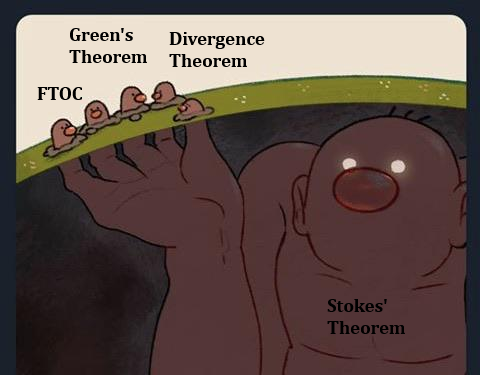
\includegraphics[width=0.45\textwidth]{chapters/chp5_pics/diglett.png}
\caption{\textit{The master of all: Stokes' Theorem}}
\label{fig:dbiglett}
\end{figure}











\newpage

\lecture{Divergence Theorem} \index{Divergence Theorem} \index{Divergence Theorem@Gauss's Theorem}

\noindent After our exploration of Stokes' Theorem and surface integrals, we now arrive at another fundamental result that connects the behavior of vector fields inside a region to their behavior on the boundary. The Divergence Theorem (also known as Gauss's Theorem) relates the flux of a vector field across a closed surface to the total divergence within the volume it encloses. This relationship proves crucial in physics—particularly in electromagnetism and fluid dynamics—where it helps us understand how fields ``flow" through space. \\

\noindent Just as Stokes' Theorem generalized Green's Theorem to surfaces in three dimensions, the Divergence Theorem extends this pattern further, connecting surface integrals to volume integrals. This progression reveals a deep pattern in vector calculus: integrals over boundaries relate to integrals over the regions they bound, regardless of dimension. We'll explore this pattern more fully after developing the theorem itself.

\subsection*{Statement and Meaning}

\noindent Throughout our studies of vector calculus, we've encountered divergence as a way to measure how much a vector field ``spreads out" at each point. A positive divergence indicates a source—a point where field lines emerge—while negative divergence signifies a sink where field lines converge. Now we'll discover a profound connection between this local behavior and the global flow across boundaries. \\

\noindent Consider a single small volume element in three-dimensional space, with a vector field $\mathbf{F}$ flowing through it. At each face of this volume, we can measure the flux—how much of the field passes through that face. The flux through each face is given by the dot product of $\mathbf{F}$ with the outward normal vector, multiplied by the area of the face. If we sum these contributions over all faces:

\[
\sum_{\text{faces}} \mathbf{F} \cdot \mathbf{n}\,d\Phi
\]

\noindent where $\mathbf{n}$ points outward from each face and $d\Phi$ represents the area of a face element, we get the net outward flux. For a small enough volume element $dV$, this flux should approximately equal the divergence within the volume multiplied by the volume:

\[
\sum_{\text{faces}} \mathbf{F} \cdot \mathbf{n}\,d\Phi \approx (\text{div }\mathbf{F})dV
\]

\noindent This local relationship suggests something deeper. Just as Green's Theorem connected boundary circulation to interior curl, here we see flux through boundaries connecting to interior divergence. Consider dividing an entire region into smaller subvolumes, as shown in Figure \ref{fig:div_volumes}. When we add up all these small volume contributions, interior faces cancel in pairs (since adjacent volumes share faces with opposite orientations), leaving only the boundary faces.

%https://commons.wikimedia.org/wiki/File:Divergence_theorem_2_-_volume_partition.png
\begin{figure}[H]
\centering
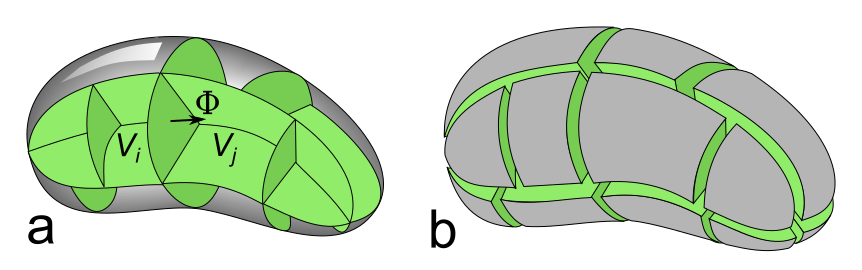
\includegraphics[width=0.8\textwidth]{chapters/chp5_pics/div_volumes.png}
\caption{\textit{(a) Adjacent subvolumes $V_i$ and $V_j$ sharing an interface $\Phi$ through which the field flows. (b) Complete subdivision of a volume showing all interfaces (green). Interior interfaces cancel in pairs, leaving only boundary contributions.}}
\label{fig:div_volumes}
\end{figure}

\noindent When two subvolumes $V_i$ and $V_j$ share an interface $\Phi$, as shown in Figure \ref{fig:div_volumes}(a), the flux through this interface appears twice in our sum—once for each subvolume but with opposite signs, since what flows out of $V_i$ must flow into $V_j$. As we sum over all subvolumes, these interior contributions cancel in pairs, leaving only the boundary faces, as visualized in Figure \ref{fig:div_volumes}(b). Taking the limit as our subdivision becomes infinitesimal, we arrive at:

\[
\oiint_S \mathbf{F} \cdot \mathbf{n}\,dS = \iiint_V \text{div }\mathbf{F}\,dV
\]

\noindent This is the Divergence Theorem. The left side measures total flux across the boundary surface $S$, while the right side accumulates the divergence throughout the volume $V$. Their equality tells us something profound: the net outward flow across any closed surface exactly equals the total ``source strength" within. \\

\noindent To make this concrete, imagine a fluid flowing through space with velocity field $\mathbf{F}$. The surface integral $\oiint_S \mathbf{F} \cdot \mathbf{n}\,dS$ measures how much fluid escapes through the boundary per unit time. Meanwhile, $\text{div }\mathbf{F}$ at each point tells us the rate at which fluid is being created (if positive) or destroyed (if negative) at that point, so $\iiint_V \text{div }\mathbf{F}\,dV$ gives the total rate of fluid generation within the volume. Their equality expresses a fundamental conservation principle: what flows out must be created within.

\subsubsection*{Gauss's Law}
\noindent This relationship extends far beyond fluid flow. In electromagnetism, when $\mathbf{F}$ is the electric field $\mathbf{E}$, the theorem becomes Gauss's law:

\[
\oiint_S \mathbf{E} \cdot \mathbf{n}\,dS = \frac{1}{\epsilon_0}\iiint_V \rho\,dV
\]

\noindent where $\rho$ is charge density and $\epsilon_0$ is a physical constant. Here $\text{div }\mathbf{E} = \rho/\epsilon_0$, relating the spreading of electric field lines to the presence of charge. Electric field lines begin on positive charges and end on negative charges—another manifestation of this deep connection between boundary behavior and interior sources. This behavior is illustrated in Figure \ref{fig:electric_field}.

\begin{figure}[H]
\centering
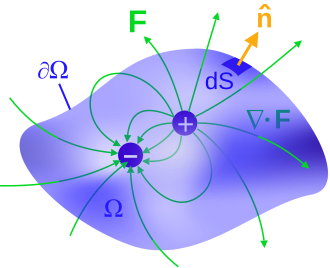
\includegraphics[width=0.4\textwidth]{chapters/chp5_pics/div_em.png}
\caption{\textit{Electric field lines (shown in green) emerging from a positive charge and terminating on a negative charge. The divergence $\nabla \cdot \mathbf{F}$ is positive near the source and negative near the sink. For any closed surface $\Omega$ (shown in blue) with surface element $dS$ and outward normal $\hat{n}$, the total flux through the surface equals the net charge enclosed, scaled by $\epsilon_0$.}}
\label{fig:electric_field}
\end{figure}

\noindent The figure shows how field lines emanate from positive charges (sources where $\nabla \cdot \mathbf{F} > 0$) and converge at negative charges (sinks where $\nabla \cdot \mathbf{F} < 0$). For any closed surface $\Omega$ enclosing these charges, the net flux through surface elements $dS$ with outward normal $\mathbf{n}$ exactly equals the enclosed charge divided by $\epsilon_0$. This provides a powerful method for calculating electric fields: if we can find a surface where symmetry makes the flux calculation simple, we can determine the field without directly solving differential equations. \\

\noindent Just as Green's Theorem connected line integrals to double integrals in the plane, the Divergence Theorem bridges surface integrals and volume integrals in space. This progression reveals a pattern: integrals over boundaries relate to integrals over the regions they bound, with the relationship governed by derivatives of the fields involved. We'll explore this pattern more fully after examining the theorem's applications and computational techniques.


\subsubsection*{Orientation and Boundary Conditions}

\noindent For the Divergence Theorem, orientation proves crucial. The surface normal $\mathbf{n}$ must point outward from the enclosed volume. This convention ensures:
\begin{itemize}
    \item Positive flux represents outward flow
    \item Negative flux represents inward flow
    \item The total signed flux captures net flow across the boundary
\end{itemize}

\noindent For a surface enclosing a volume, we can determine the outward normal at any point through the right hand rule.

\subsubsection*{Computational Forms and Strategy}

\noindent Just as we expanded Stokes' Theorem into component forms, we can make the Divergence Theorem more computationally accessible. Recall that for a vector field $\mathbf{F} = P\mathbf{i} + Q\mathbf{j} + R\mathbf{k}$:

\[
\text{div }\mathbf{F} = \nabla \cdot \mathbf{F} = \frac{\partial P}{\partial x} + \frac{\partial Q}{\partial y} + \frac{\partial R}{\partial z}
\]

\noindent Therefore, the Divergence Theorem becomes:
\[
\oiint_S \mathbf{F} \cdot \mathbf{n}\,dS = \iiint_V \left(\frac{\partial P}{\partial x} + \frac{\partial Q}{\partial y} + \frac{\partial R}{\partial z}\right)\,dV
\]

\noindent The surface integral on the left requires careful consideration of the outward unit normal $\mathbf{n}$. For different types of surfaces, we have:

\begin{enumerate}
    \item \textbf{Level Surfaces:} For a surface $f(x,y,z) = c$:
    \[
    \mathbf{n} = \frac{\nabla f}{\|\nabla f\|} = \frac{1}{\|\nabla f\|}\left\langle\frac{\partial f}{\partial x}, \frac{\partial f}{\partial y}, \frac{\partial f}{\partial z}\right\rangle
    \]
    
    \item \textbf{Parametric Surfaces:} For $\mathbf{r}(u,v) = \langle x(u,v), y(u,v), z(u,v) \rangle$:
    \[
    \mathbf{n} = \frac{\mathbf{r}_u \times \mathbf{r}_v}{\|\mathbf{r}_u \times \mathbf{r}_v\|}
    \]
    
    \item \textbf{Simple Surfaces:} For surfaces like $z = g(x,y)$:
    \[
    \mathbf{n} = \frac{\langle-g_x, -g_y, 1\rangle}{\sqrt{1 + g_x^2 + g_y^2}}
    \]
\end{enumerate}

\noindent In different coordinate systems, the divergence takes special forms:

\begin{itemize}
    \item \textbf{Cylindrical Coordinates} $(r,\theta,z)$:
    \[
    \text{div }\mathbf{F} = \frac{1}{r}\frac{\partial}{\partial r}(rF_r) + \frac{1}{r}\frac{\partial F_\theta}{\partial \theta} + \frac{\partial F_z}{\partial z}
    \]
    
    \item \textbf{Spherical Coordinates} $(r,\theta,\phi)$:
    \[
    \text{div }\mathbf{F} = \frac{1}{r^2}\frac{\partial}{\partial r}(r^2F_r) + \frac{1}{r\sin\theta}\frac{\partial}{\partial \theta}(\sin\theta F_\theta) + \frac{1}{r\sin\theta}\frac{\partial F_\phi}{\partial \phi}
    \]
\end{itemize}

\noindent When choosing which form to use, consider:

\begin{itemize}
    \item Symmetry of the vector field
    \item Shape of the boundary surface
    \item Complexity of the divergence versus the surface integral
\end{itemize}

\noindent For example, if the region is a sphere and the field has spherical symmetry, using spherical coordinates often simplifies the calculation dramatically. Similarly, for cylindrical bodies, cylindrical coordinates typically prove most efficient. \\

\noindent A systematic approach to these problems involves:

\begin{enumerate}
    \item Identify the vector field components and the boundary surface
    \item Choose appropriate coordinates based on symmetry
    \item Determine whether surface or volume integral is simpler
    \item If using surface integral:
        \begin{itemize}
            \item Break surface into pieces if necessary
            \item Calculate normal vectors for each piece
            \item Set up parameterization if needed
        \end{itemize}
    \item If using volume integral:
        \begin{itemize}
            \item Calculate divergence explicitly
            \item Determine integration bounds
            \item Consider coordinate transformations
        \end{itemize}
\end{enumerate}

\noindent This framework provides a practical approach to applying the Divergence Theorem, turning the abstract relationship between flux and divergence into concrete computational steps.


\exampleline
\begin{example}
Consider the vector field $\mathbf{F}(x,y,z) = (x^2y)\mathbf{i} + (y^2z)\mathbf{j} + (z^2x)\mathbf{k}$, and let $V$ be the region bounded by the paraboloid $z = x^2 + y^2$ and the plane $z = 1$. Verify the Divergence Theorem by computing both:
\begin{enumerate}
    \item The surface integral $\oiint_S \mathbf{F} \cdot \mathbf{n}\,dS$
    \item The volume integral $\iiint_V \text{div }\mathbf{F}\,dV$
\end{enumerate}

\begin{solution}
\begin{enumerate}
\item \textbf{Surface Integral}

The boundary $S$ consists of two pieces:
\begin{itemize}
    \item $S_1$: The paraboloid $z = x^2 + y^2$ (bottom)
    \item $S_2$: The plane $z = 1$ (top)
\end{itemize}

For $S_1$ (paraboloid):
\begin{itemize}
    \item Writing as $f(x,y,z) = z - x^2 - y^2 = 0$, the gradient is $\nabla f = \langle-2x, -2y, 1\rangle$
    \item Since our region $V$ is above this surface, the outward normal must point downward:
    \[
    \mathbf{n}_1 = \frac{\langle 2x, 2y, -1 \rangle}{\sqrt{4x^2 + 4y^2 + 1}}
    \]
    \item The flux integral becomes:
    \begin{align*}
    \iint_{S_1} \mathbf{F} \cdot \mathbf{n}_1\,dS &= \iint_D \frac{2x^3y + 2y^3z - z^2x}{\sqrt{4x^2 + 4y^2 + 1}}\sqrt{4x^2 + 4y^2 + 1}\,dA \\
    &= \iint_D (2x^3y + 2y^3(x^2 + y^2) - x(x^2 + y^2)^2)\,dA
    \end{align*}
    where $D$ is the projection onto the $xy$-plane bounded by $x^2 + y^2 \leq 1$
\end{itemize}

For $S_2$ (plane):
\begin{itemize}
    \item Since our region $V$ is below this surface, the outward normal on the top cap points upward:
    \[
    \mathbf{n}_2 = \mathbf{k}
    \]
    \item The flux integral is:
    \[
    \iint_{S_2} \mathbf{F} \cdot \mathbf{n}_2\,dS = \iint_D z^2x\big|_{z=1}\,dA = \iint_D x\,dA
    \]
\end{itemize}

Converting both integrals to polar coordinates:
\begin{itemize}
    \item $x = r\cos\theta$, $y = r\sin\theta$
    \item For $S_1$: $z = r^2$
    \item For $S_2$: $z = 1$
    \item Bounds: $0 \leq r \leq 1$, $0 \leq \theta \leq 2\pi$
\end{itemize}

\begin{align*}
\iint_{S_1} \mathbf{F} \cdot \mathbf{n}_1\,dS &= \int_0^{2\pi}\int_0^1 (2r^4\cos^3\theta\sin\theta + 2r^5\sin^3\theta - r^5\cos\theta)r\,dr\,d\theta \\
&= 0 \text{ (odd functions over }[0,2\pi]\text{)}
\end{align*}

\begin{align*}
\iint_{S_2} \mathbf{F} \cdot \mathbf{n}_2\,dS &= \int_0^{2\pi}\int_0^1 r\cos\theta\,r\,dr\,d\theta = 0
\end{align*}

Therefore, the total surface integral is zero.

\item \textbf{Volume Integral}

First, calculate $\text{div }\mathbf{F}$:
\begin{align*}
\text{div }\mathbf{F} &= \frac{\partial}{\partial x}(x^2y) + \frac{\partial}{\partial y}(y^2z) + \frac{\partial}{\partial z}(z^2x) \\
&= 2xy + 2yz + 2zx
\end{align*}

Setting up the volume integral in cylindrical coordinates:
\begin{itemize}
    \item $x = r\cos\theta$, $y = r\sin\theta$
    \item Lower bound: $z = r^2$
    \item Upper bound: $z = 1$
    \item Radial bound: $0 \leq r \leq 1$
\end{itemize}

\begin{align*}
\iiint_V \text{div }\mathbf{F}\,dV &= \int_0^{2\pi}\int_0^1\int_{r^2}^1 (2r^2\cos\theta\sin\theta + 2rz\sin\theta + 2rz\cos\theta)r\,dz\,dr\,d\theta \\
&= \int_0^{2\pi}\int_0^1\int_{r^2}^1 2r(r\sin\theta\cos\theta + z(\sin\theta + \cos\theta))\,dz\,dr\,d\theta \\
&= 0 \text{ (by symmetry)}
\end{align*}
\end{enumerate}

\noindent Therefore, both sides of the Divergence Theorem equal zero, confirming the theorem's validity for this case. \\

\noindent \textbf{Physical Interpretation:} The fact that both integrals equal zero suggests that any flow entering the region through one part of the boundary must exit through another part, with no net accumulation or depletion within the volume. This is analogous to an incompressible fluid flow, where the total inflow must equal the total outflow.
\end{solution}
\end{example}
\exampleline

\subsection*{Physical Applications} \index{Conservation Laws}

\noindent The Divergence Theorem finds its deepest expression in physical conservation laws, where it bridges local field behavior with global measurements of flow and flux. At its heart lies a profound connection: what flows through a boundary must be created or destroyed within. This principle manifests throughout physics in increasingly sophisticated ways. \\

\noindent Consider first the flow of mass in a fluid. At each point in space and time, we have a density $\rho(x,y,z,t)$ and a velocity field $\mathbf{v}$ that tells us how the fluid moves. The product $\rho\mathbf{v}$ represents mass flux—the flow of mass through space. Conservation of mass demands that any change in the total mass within a volume must precisely balance the flow through its boundary:

\[
\frac{d}{dt}\iiint_V \rho\,dV = -\oiint_S \rho\mathbf{v} \cdot \mathbf{n}\,dS
\]

\noindent The Divergence Theorem transforms this global statement into a local one. Bringing the time derivative inside the volume integral and applying the theorem to the right side:

\[
\iiint_V \frac{\partial \rho}{\partial t}\,dV = -\iiint_V \text{div}(\rho\mathbf{v})\,dV
\]

\noindent Since this equality must hold for any volume, we obtain the continuity equation:

\[
\frac{\partial \rho}{\partial t} + \text{div}(\rho\mathbf{v}) = 0
\]

\noindent For incompressible fluids where density remains constant, this reduces to $\text{div }\mathbf{v} = 0$, expressing that the velocity field has no sources or sinks. \\

\noindent This pattern extends beautifully to electromagnetism. Electric charge serves as the source of electromagnetic fields, and its conservation takes a similar mathematical form. If $\mathbf{J}$ represents current density—the flow of charge through space—and $\rho$ now represents charge density, conservation of charge requires:

\[
\text{div }\mathbf{J} = -\frac{\partial \rho}{\partial t}
\]

\noindent This equation tells us something profound: changes in charge distribution necessitate current flow. Moreover, when combined with Maxwell's equations, particularly Gauss's law $\text{div }\mathbf{E} = \rho/\epsilon_0$, it leads to the prediction of electromagnetic waves. The interplay between changing charge distributions and current flow creates ripples in the electromagnetic field that propagate through space. \\

\noindent Heat transfer provides yet another manifestation of these principles. When heat flows through a material, the heat flux $\mathbf{q}$ relates to temperature changes through:

\[
\text{div }\mathbf{q} = -c\rho\frac{\partial T}{\partial t}
\]

\noindent where $c$ represents specific heat capacity and $T(x,y,z,t)$ is the temperature field. This equation encodes Fourier's insight that heat flows from hot to cold regions, with the rate of temperature change determined by material properties. The divergence of heat flux directly drives local temperature evolution. \\

\noindent These seemingly distinct phenomena share a deep mathematical structure. For any conserved quantity $\psi$ with associated flux $\mathbf{F}$, conservation takes the form:

\[
\frac{\partial \psi}{\partial t} + \text{div }\mathbf{F} = 0
\]

\noindent Integrating over a volume and applying the Divergence Theorem reveals the universal pattern:

\[
\frac{d}{dt}\iiint_V \psi\,dV = -\oiint_S \mathbf{F} \cdot \mathbf{n}\,dS
\]

\noindent This structure appears in momentum conservation, where stress tensors describe force transmission through materials. It governs energy conservation in fields, where Poynting vectors track energy flow through space. Even quantum mechanics obeys this pattern—probability current ensures that quantum particles are neither created nor destroyed during evolution. \\

\noindent The Divergence Theorem thus emerges as one of physics' most profound results. It provides the mathematical framework for expressing nature's conservation principles, connecting microscopic behavior to macroscopic measurements. Whether describing fluid flow, electromagnetic fields, heat transfer, or quantum systems, the theorem reveals how local changes in fields relate to global flows across boundaries—a fundamental unity underlying diverse physical phenomena.


\exampleline
\begin{example}  \textbf{Final Boss}
A solid sphere of radius $R$ has density given by $\rho(r) = \rho_0\left(1 - \frac{r^2}{R^2}\right)$, where $\rho_0$ is a constant and $r$ is the distance from the center. Using the Divergence Theorem, prove that:

\begin{enumerate}
    \item The gravitational field inside the sphere at distance $r$ from the center is $\mathbf{g}(r) = -\frac{4\pi G\rho_0}{3}\left(1 - \frac{3r^2}{5R^2}\right)r\hat{\mathbf{r}}$
    \item The gravitational potential $\Phi(r)$ satisfies Poisson's equation: $\nabla^2\Phi = 4\pi G\rho$
    \item The gravitational field outside the sphere is identical to that of a point mass located at the center with mass equal to the total mass of the sphere
\end{enumerate}

\noindent Hint: The gravitational potential $\Phi$ at a point $\mathbf{r}$ due to a mass distribution is given by:
\[
\Phi(\mathbf{r}) = -G\iiint_V \frac{\rho(\mathbf{r'})}{|\mathbf{r} - \mathbf{r'}|} dV'
\]

\noindent The gravitational field is related to the potential by $\mathbf{g} = -\nabla\Phi$. The Divergence Theorem can be applied to gravitational fields through the relationship $\nabla \cdot \mathbf{g} = -4\pi G\rho$, which relates the divergence of the gravitational field to the mass density. For a spherically symmetric situation, this means $\oiint_{S_r} \mathbf{g} \cdot \mathbf{n} \, dS = g(r) \cdot 4\pi r^2 = -4\pi G M_{enclosed}$, where $M_{enclosed}$ is the mass contained within radius $r$. \\


\begin{solution}
We'll solve this problem by applying the Divergence Theorem to the gravitational field, revealing fundamental properties of gravity.

\begin{enumerate}
    \item \textbf{Gravitational Field Inside the Sphere}
    
    First, note that the gravitational field $\mathbf{g}$ is related to the gravitational potential $\Phi$ by:
    \[
    \mathbf{g} = -\nabla\Phi
    \]
    
    By Newton's law of gravitation and the principle of superposition, the potential at a point $\mathbf{r}$ due to a mass distribution is:
    \[
    \Phi(\mathbf{r}) = -G\iiint_V \frac{\rho(\mathbf{r'})}{|\mathbf{r} - \mathbf{r'}|} dV'
    \]
    
    For a spherically symmetric density distribution, the field must be radial: $\mathbf{g} = g(r)\hat{\mathbf{r}}$. To determine $g(r)$, we'll apply the Divergence Theorem to a sphere of radius $r < R$.
    
    From Gauss's law for gravity:
    \[
    \oiint_S \mathbf{g} \cdot \mathbf{n} \, dS = -4\pi G M_{enc}
    \]
    
    where $M_{enc}$ is the mass enclosed by the sphere of radius $r$. The left side is:
    \[
    \oiint_S \mathbf{g} \cdot \mathbf{n} \, dS = \oiint_S g(r)\hat{\mathbf{r}} \cdot \hat{\mathbf{r}} \, dS = g(r) \cdot 4\pi r^2
    \]
    
    The enclosed mass is:
    \[
    \begin{aligned}
    M_{enc} &= \iiint_{r' \leq r} \rho(r') \, dV' \\
    &= \int_0^{2\pi} \int_0^{\pi} \int_0^r \rho_0\left(1 - \frac{r'^2}{R^2}\right)r'^2 \sin\theta \, dr' \, d\theta \, d\phi \\
    &= 4\pi\rho_0 \int_0^r \left(1 - \frac{r'^2}{R^2}\right)r'^2 \, dr' \\
    &= 4\pi\rho_0 \left(\frac{r^3}{3} - \frac{r^5}{5R^2}\right)
    \end{aligned}
    \]
    
    Equating the surface integral with $-4\pi G M_{enc}$:
    \[
    \begin{aligned}
    g(r) \cdot 4\pi r^2 &= -4\pi G \cdot 4\pi\rho_0 \left(\frac{r^3}{3} - \frac{r^5}{5R^2}\right) \\
    g(r) &= -\frac{4\pi G\rho_0}{r^2} \left(\frac{r^3}{3} - \frac{r^5}{5R^2}\right) \\
    &= -\frac{4\pi G\rho_0}{3}\left(1 - \frac{3r^2}{5R^2}\right)r
    \end{aligned}
    \]
    
    Therefore:
    \[
    \mathbf{g}(r) = -\frac{4\pi G\rho_0}{3}\left(1 - \frac{3r^2}{5R^2}\right)r\hat{\mathbf{r}} \quad \text{for } r \leq R
    \]
    
    \item \textbf{Verification of Poisson's Equation}
    
    Poisson's equation for gravity states:
    \[
    \nabla^2\Phi = 4\pi G\rho
    \]
    
    Since $\mathbf{g} = -\nabla\Phi$, we have $\nabla \cdot \mathbf{g} = -\nabla^2\Phi$. To verify Poisson's equation, we need to show that:
    \[
    \nabla \cdot \mathbf{g} = -4\pi G\rho
    \]
    
    For a radial vector field $\mathbf{g} = g(r)\hat{\mathbf{r}}$, the divergence in spherical coordinates is:
    \[
    \nabla \cdot \mathbf{g} = \frac{1}{r^2}\frac{\partial}{\partial r}(r^2 g(r))
    \]
    
    Substituting $g(r) = -\frac{4\pi G\rho_0}{3}\left(1 - \frac{3r^2}{5R^2}\right)r$:
    \[
    \begin{aligned}
    \nabla \cdot \mathbf{g} &= \frac{1}{r^2}\frac{\partial}{\partial r}\left[r^2 \cdot \left(-\frac{4\pi G\rho_0}{3}\left(1 - \frac{3r^2}{5R^2}\right)r\right)\right] \\
    &= \frac{1}{r^2}\frac{\partial}{\partial r}\left[-\frac{4\pi G\rho_0}{3}r^3\left(1 - \frac{3r^2}{5R^2}\right)\right] \\
    &= \frac{1}{r^2}\frac{\partial}{\partial r}\left[-\frac{4\pi G\rho_0}{3}r^3 + \frac{4\pi G\rho_0}{5R^2}r^5\right] \\
    &= \frac{1}{r^2}\left[-\frac{4\pi G\rho_0}{3} \cdot 3r^2 + \frac{4\pi G\rho_0}{5R^2} \cdot 5r^4\right] \\
    &= -4\pi G\rho_0 + \frac{4\pi G\rho_0r^2}{R^2} \\
    &= -4\pi G\rho_0\left(1 - \frac{r^2}{R^2}\right) \\
    &= -4\pi G\rho(r)
    \end{aligned}
    \]
    
    This confirms that the gravitational field satisfies Poisson's equation $\nabla^2\Phi = 4\pi G\rho$.
    
    \item \textbf{External Gravitational Field}
    
    For $r > R$, we'll again use the Divergence Theorem in the form of Gauss's law for gravity.
    
    The total mass of the sphere is:
    \[
    \begin{aligned}
    M_{total} &= \iiint_V \rho(r) \, dV \\
    &= 4\pi\rho_0 \int_0^R \left(1 - \frac{r^2}{R^2}\right)r^2 \, dr \\
    &= 4\pi\rho_0 \left[\frac{r^3}{3} - \frac{r^5}{5R^2}\right]_0^R \\
    &= 4\pi\rho_0R^3 \left(\frac{1}{3} - \frac{1}{5}\right) \\
    &= 4\pi\rho_0R^3 \cdot \frac{2}{15} = \frac{8\pi\rho_0R^3}{15}
    \end{aligned}
    \]
    
    By symmetry, the gravitational field outside the sphere must be radial. Applying Gauss's law to a sphere of radius $r > R$:
    \[
    \oiint_S \mathbf{g} \cdot \mathbf{n} \, dS = -4\pi GM_{total}
    \]
    
    The left side equals $g(r) \cdot 4\pi r^2$, so:
    \[
    \begin{aligned}
    g(r) \cdot 4\pi r^2 &= -4\pi G \cdot \frac{8\pi\rho_0R^3}{15} \\
    g(r) &= -\frac{GM_{total}}{r^2} = -G \cdot \frac{8\pi\rho_0R^3}{15} \cdot \frac{1}{r^2}
    \end{aligned}
    \]
    
    Therefore:
    \[
    \mathbf{g}(r) = -G \cdot \frac{8\pi\rho_0R^3}{15} \cdot \frac{\hat{\mathbf{r}}}{r^2} = -\frac{GM_{total}}{r^2}\hat{\mathbf{r}} \quad \text{for } r \geq R
    \]
    
    This is identical to the gravitational field of a point mass $M_{total}$ located at the center, confirming Newton's Shell Theorem: the gravitational field outside a spherically symmetric mass distribution is the same as if all the mass were concentrated at the center.
\end{enumerate}

\end{solution}
\end{example}
\exampleline

\subsection*{Choosing the Right Theorem}
\noindent The three major integral theorems each convert between different types of integrals. Here is a quick guide:\\ \\
\begin{itemize}
\item \textbf{Green's Theorem:} Converts a line integral around a closed curve in the plane to a double integral over the enclosed region (or vice versa).
\item \textbf{Stokes' Theorem:} Converts a line integral around a closed curve in 3D to a surface integral of the curl over any surface bounded by that curve (or vice versa).
\item \textbf{Divergence Theorem:} Converts a flux integral over a closed surface to a triple integral of the divergence over the enclosed volume (or vice versa).
\item \textbf{Fundamental Theorem for Line Integrals:} If the field is conservative (\(\mathbf{F} = \nabla f\)), the line integral depends only on the endpoints: \(\int_C \mathbf{F} \cdot d\mathbf{r} = f(\mathbf{B}) - f(\mathbf{A})\).
\end{itemize}
\noindent \textbf{Strategy:} If one side of the equation is hard to compute directly, use the theorem to convert it to the other side.


\newpage

\formsdefs{}

\subsection*{Important Vocabulary}
\begin{itemize}
    \item \textbf{Vector Field:} A function that assigns a vector to each point in space, written as $\mathbf{F}(x,y,z) = P\mathbf{i} + Q\mathbf{j} + R\mathbf{k}$.

    \item \textbf{Conservative Field:} A vector field that can be written as the gradient of some scalar function $f$, where $\mathbf{F} = \nabla f$.

    \item \textbf{Curl:} A measure of rotation in a vector field, given by $\text{curl }\mathbf{F} = \nabla \times \mathbf{F}$.

    \item \textbf{Divergence:} A measure of the outward flux per unit volume in a vector field, given by $\text{div }\mathbf{F} = \nabla \cdot \mathbf{F}$.

    \item \textbf{Line Integral:} The integral of a vector field along a curve $C$, measuring quantities like work: $\int_C \mathbf{F} \cdot d\mathbf{r}$.

    \item \textbf{Surface Integral:} The integral of a vector field over a surface $S$, measuring flux: $\iint_S \mathbf{F} \cdot d\mathbf{S}$.

    \item \textbf{Flux:} The rate of flow of a vector field through a surface, measured by surface integrals.

    \item \textbf{Orientable Surface:} A surface where a consistent normal vector direction can be defined at each point.

    \item \textbf{Potential Function:} A scalar function $f$ whose gradient gives a conservative vector field.

    \item \textbf{Path Independence:} Property of conservative fields where line integrals depend only on endpoints, not the path taken.

    \item \textbf{Source:} Point where field lines emerge (positive divergence).

    \item \textbf{Sink:} Point where field lines converge (negative divergence).

    \item \textbf{Circulation:} The line integral of a vector field around a closed curve, measuring the tendency of the field to flow along the curve.

    \item \textbf{Simply Connected Domain:} A region with no holes, meaning every closed curve in the region can be continuously shrunk to a point without leaving the region.

    \item \textbf{Closed Surface:} A surface with no boundary that fully encloses a volume, such as a sphere or the surface of a cube.
\end{itemize}

\subsection*{Key Formulas}
\begin{multicols}{2}

\paragraph{Scalar Line Integral}
\[
\int_C f\,ds = \int_a^b f(\mathbf{r}(t))\,\|\mathbf{r}'(t)\|\,dt
\]
Direction does not matter: $\int_C f\,ds = \int_{-C} f\,ds$.

\paragraph{Vector Field Line Integral}
\[
\int_C \mathbf{F}\cdot d\mathbf{r} = \int_a^b \mathbf{F}(\mathbf{r}(t))\cdot\mathbf{r}'(t)\,dt
\]
Also written $\int_C P\,dx + Q\,dy + R\,dz$.\\
Direction matters: $\int_{-C} = -\int_C$.

\paragraph{Fundamental Theorem for Line Integrals}
If $\mathbf{F} = \nabla f$ (conservative), $C$ from $A$ to $B$:
\[
\int_C \nabla f\cdot d\mathbf{r} = f(B) - f(A)
\]
Path-independent; $\oint_C \nabla f\cdot d\mathbf{r} = 0$.

\paragraph{Conservative Field Test}
On a simply connected domain, $\mathbf{F} = \langle P,Q,R\rangle$ is conservative iff:
\[
P_y = Q_x, \quad P_z = R_x, \quad Q_z = R_y
\]
In 2D: $P_y = Q_x$ suffices.

\paragraph{Finding the Potential Function}
Integrate $f_x = P$ w.r.t.\ $x$ ($+g(y,z)$); differentiate and match $f_y = Q$ to find $g$; repeat for $z$.

\paragraph{Green's Theorem}
$C$ simple closed (CCW), $D$ interior:
\[
\oint_C P\,dx + Q\,dy = \iint_D\!\left(\frac{\partial Q}{\partial x} - \frac{\partial P}{\partial y}\right)dA
\]
Area: $A = \frac{1}{2}\oint_C(x\,dy - y\,dx)$.

\paragraph{Curl (3D)}
\[
\nabla\times\mathbf{F} = \begin{vmatrix}\mathbf{i}&\mathbf{j}&\mathbf{k}\\ \partial_x & \partial_y & \partial_z \\ P & Q & R\end{vmatrix} = \langle R_y\!-\!Q_z,\; P_z\!-\!R_x,\; Q_x\!-\!P_y\rangle
\]
2D curl (scalar): $Q_x - P_y$ (the $\mathbf{k}$-component).

\paragraph{Divergence}
\[
\nabla\cdot\mathbf{F} = P_x + Q_y + R_z
\]
$>0$: source, $<0$: sink, $=0$: incompressible.

\paragraph{Key Identities}
\begin{align*}
\nabla\times(\nabla f) &= \mathbf{0} \quad\text{(curl of gradient)}\\
\nabla\cdot(\nabla\times\mathbf{F}) &= 0 \quad\text{(div of curl)}\\
\nabla^2 f &= f_{xx}+f_{yy}+f_{zz} \quad\text{(Laplacian)}
\end{align*}

\paragraph{Product Rules}
\begin{align*}
\nabla(fg) &= f\nabla g + g\nabla f\\
\nabla\cdot(f\mathbf{F}) &= f(\nabla\cdot\mathbf{F}) + \mathbf{F}\cdot\nabla f\\
\nabla\times(f\mathbf{F}) &= f(\nabla\times\mathbf{F}) + \nabla f\times\mathbf{F}
\end{align*}

\paragraph{Parametric Surfaces}
$\mathbf{r}(u,v) = \langle x(u,v),y(u,v),z(u,v)\rangle$\\
Normal: $\mathbf{n} = \mathbf{r}_u\times\mathbf{r}_v$\\
$dS = \|\mathbf{r}_u\times\mathbf{r}_v\|\,du\,dv$

\paragraph{Common Surface Elements}
\begin{align*}
z = g(x,y)&: \; dS = \sqrt{1+g_x^2+g_y^2}\,dA\\
\text{Sphere } a&: \; dS = a^2\sin\phi\,d\phi\,d\theta\\
\text{Cylinder } R&: \; dS = R\,d\theta\,dz
\end{align*}

\paragraph{Scalar Surface Integral}
\[
\iint_S f\,dS = \iint_D f(\mathbf{r}(u,v))\,\|\mathbf{r}_u\times\mathbf{r}_v\|\,du\,dv
\]
$f=1$ gives surface area.

\paragraph{Flux (Vector Surface Integral)}
\[
\iint_S \mathbf{F}\cdot d\mathbf{S} = \iint_D \mathbf{F}\cdot(\mathbf{r}_u\times\mathbf{r}_v)\,du\,dv
\]
For $z = g(x,y)$ with upward normal:
\[
\iint_S \mathbf{F}\cdot d\mathbf{S} = \iint_D(-Pg_x - Qg_y + R)\,dA
\]

\paragraph{Stokes' Theorem}
$S$ oriented surface, $C$ boundary (right-hand rule):
\[
\oint_C \mathbf{F}\cdot d\mathbf{r} = \iint_S(\nabla\times\mathbf{F})\cdot\mathbf{n}\,dS
\]
Green's Theorem is the special case $S$ flat in $xy$.

\paragraph{Divergence Theorem}
$S$ closed surface (outward normal), $V$ interior:
\[
\oiint_S \mathbf{F}\cdot\mathbf{n}\,dS = \iiint_V(\nabla\cdot\mathbf{F})\,dV
\]

\paragraph{Generalized Stokes' Theorem}
\[
\int_\Omega d\omega = \int_{\partial\Omega}\omega
\]
Unifies FTOC, FTOLI, Green's, Stokes', Divergence.

\paragraph{Maxwell's Equations}
\begin{align*}
\nabla\cdot\mathbf{E} &= \rho/\epsilon_0 & \nabla\times\mathbf{E} &= -\partial_t\mathbf{B}\\
\nabla\cdot\mathbf{B} &= 0 & \nabla\times\mathbf{B} &= \mu_0\mathbf{J}+\mu_0\epsilon_0\partial_t\mathbf{E}
\end{align*}

\end{multicols}

\begin{table}[H]
\centering
\begin{tabular}{|c|c|c|}
\hline
\textbf{Operator} & \textbf{Cylindrical} $(r,\theta,z)$ & \textbf{Spherical} $(r,\theta,\phi)$ \\
\hline
\rule{0pt}{4ex}
$\nabla f$ & $\displaystyle\frac{\partial f}{\partial r}\mathbf{e}_r + \frac{1}{r}\frac{\partial f}{\partial \theta}\mathbf{e}_\theta + \frac{\partial f}{\partial z}\mathbf{e}_z$ & $\displaystyle\frac{\partial f}{\partial r}\mathbf{e}_r + \frac{1}{r}\frac{\partial f}{\partial \theta}\mathbf{e}_\theta + \frac{1}{r\sin\theta}\frac{\partial f}{\partial \phi}\mathbf{e}_\phi$ \\[2ex]
\hline
\rule{0pt}{4ex}
$\nabla \cdot \mathbf{F}$ & $\displaystyle\frac{1}{r}\frac{\partial}{\partial r}(rF_r) + \frac{1}{r}\frac{\partial F_\theta}{\partial \theta} + \frac{\partial F_z}{\partial z}$ & $\displaystyle\frac{1}{r^2}\frac{\partial}{\partial r}(r^2F_r) + \frac{1}{r\sin\theta}\frac{\partial}{\partial \theta}(\sin\theta F_\theta) + \frac{1}{r\sin\theta}\frac{\partial F_\phi}{\partial \phi}$ \\[2ex]
\hline
\rule{0pt}{6ex}
$\nabla \times \mathbf{F}$ & $\begin{pmatrix}
\frac{1}{r}\frac{\partial F_z}{\partial \theta} - \frac{\partial F_\theta}{\partial z} \\[1ex]
\frac{\partial F_r}{\partial z} - \frac{\partial F_z}{\partial r} \\[1ex]
\frac{1}{r}\frac{\partial}{\partial r}(rF_\theta) - \frac{1}{r}\frac{\partial F_r}{\partial \theta}
\end{pmatrix}$ & $\begin{pmatrix}
\frac{1}{r\sin\theta}\left(\frac{\partial}{\partial \theta}(\sin\theta F_\phi) - \frac{\partial F_\theta}{\partial \phi}\right) \\[1ex]
\frac{1}{r}\left(\frac{1}{\sin\theta}\frac{\partial F_r}{\partial \phi} - \frac{\partial}{\partial r}(rF_\phi)\right) \\[1ex]
\frac{1}{r}\left(\frac{\partial}{\partial r}(rF_\theta) - \frac{\partial F_r}{\partial \theta}\right)
\end{pmatrix}$ \\[6ex]
\hline
\end{tabular}
\end{table}


\newpage


\practice{}

\begin{multicols}{2}

\begin{enumerate}
%lect 1
% 1
\item 
Consider the 2D vector field
\[
\mathbf{F}(x,y) = (x+1)\mathbf{i} + (y-2)\mathbf{j}.
\]
\begin{enumerate}
\item Evaluate \(\mathbf{F}(1,-1)\).
\item Sketch a few representative vectors near the origin to see how this field behaves.
\end{enumerate}

% 2
\item 
Explain the difference between a \emph{scalar field} and a \emph{vector field}. Give one concrete physical example of each (e.g., temperature distribution for a scalar field, velocity flow for a vector field).

% 3
\item 
Given
\[
\mathbf{F}(x,y) = -y\mathbf{i} + x\mathbf{j},
\]
describe in words how you would plot the arrows at the points \((2,0)\), \((1,1)\), and \((-2,-2)\). What does the overall pattern of the field suggest?

% 4
\item 
Consider the vector field
\[
\mathbf{F}(x,y) = \bigl(e^x,\, e^y\bigr).
\]
\begin{enumerate}
\item Evaluate \(\mathbf{F}(0,0)\) and \(\mathbf{F}(1,2)\).
\item Based on these vectors, does the origin appear to be a source, a sink, or neither? Give a brief reason.
\end{enumerate}

% 5 (old #3)
\item \enspace
A 3D vector field is given by
    \begin{multline*}
\mathbf{G}(x,y,z) = \frac{x}{x^2 + y^2 + z^2} \,\mathbf{i} + \\
\frac{y}{x^2 + y^2 + z^2} \,\mathbf{j} + \frac{z}{x^2 + y^2 + z^2} \,\mathbf{k}.
    \end{multline*}
Is \(\mathbf{G}\) continuous everywhere in \(\mathbb{R}^3\)? If not, identify any problematic points.

% 6
\item 
Consider the 3D vector field
\[
\mathbf{H}(x,y,z) = x^2\,\mathbf{i} \;+\; y^2\,\mathbf{j} \;+\; z^2\,\mathbf{k}.
\]
\begin{enumerate}
\item Determine whether \(\mathbf{H}\) is continuous at all points in \(\mathbb{R}^3\).
\item If there are any problematic points, identify them and explain why.
\end{enumerate}

% 7
\item 
Explain briefly why engineers or physicists might choose to visualize a vector field with all arrows having the same length (i.e., \emph{normalized}). Give one advantage and one disadvantage of this approach, referencing physical interpretations.

% 8
\item \enspace
Classify the origin for each of the following vector fields:
\begin{enumerate}
\item $\mathbf{F}_1(x,y) = x\,\mathbf{i} + y\,\mathbf{j}$
\item $\mathbf{F}_2(x,y) = -x\,\mathbf{i} - y\,\mathbf{j}$
\item $\mathbf{F}_3(x,y) = x\,\mathbf{i} - y\,\mathbf{j}$
\end{enumerate}
State which is a source, which is a sink, and which is a saddle.

% 9
\item \enspace
Show that the 2D vector field
\[
\mathbf{F}(x,y) = y\,\mathbf{i} \;-\; x\,\mathbf{j}
\]
is \emph{not} conservative by using the partial-derivative condition
\(\tfrac{\partial P}{\partial y} \neq \tfrac{\partial Q}{\partial x}\).
In one sentence, relate this to the ``rotational'' or ``circulatory'' pattern you see near the origin.

% 10
\item \enspace
Let
\[
\mathbf{F}(x,y) = x^3\,\mathbf{i} + 3x^2y\,\mathbf{j}.
\]
\begin{enumerate}
\item Use the condition \(\tfrac{\partial P}{\partial y} = \tfrac{\partial Q}{\partial x}\) to determine if \(\mathbf{F}\) is conservative.
\item If it \emph{is} conservative, find a potential function \(f(x,y)\) such that \(\nabla f = \mathbf{F}\).
\end{enumerate}

% 11
\item \enspace
Consider the 3D field
\[
\mathbf{F}(x,y,z) = 2xy\,\mathbf{i} + \bigl(x^2 + z^2\bigr)\mathbf{j} + 2yz\,\mathbf{k}.
\]
Test whether \(\mathbf{F}\) is conservative by checking the equality of appropriate mixed partial derivatives in \(\mathbb{R}^3\).

% 12
\item \enspace
For the 2D field
\[
\mathbf{F}(x,y) = \sqrt{x^2 + y^2}\,\mathbf{i}
\;-\;
\bigl(\sin(xy)\bigr)\,\mathbf{j},
\]
compute:
\[
\tfrac{\partial P}{\partial x}, \quad \tfrac{\partial P}{\partial y}, \quad
\tfrac{\partial Q}{\partial x}, \quad \tfrac{\partial Q}{\partial y}.
\]
Which (if any) of these partial derivatives are undefined at the origin?

% 13
\item \enspace
Consider the 2D vector field
\[
\mathbf{F}(x,y) = \bigl(x^2 + y^2\bigr)\mathbf{i}
\;-\;
\bigl(x^2 + y^2\bigr)\mathbf{j}.
\]
\begin{enumerate}
\item Check whether \(\mathbf{F}\) is conservative by comparing \(\tfrac{\partial P}{\partial y}\) and \(\tfrac{\partial Q}{\partial x}\).
\item If it \emph{is} conservative, find a potential function. If not, classify the origin as a source, sink, or saddle.
\end{enumerate}

%lect 2

\item 
Compute the scalar line integral
\[
\int_C (x + y)\,ds
\]
where \(C\) is the line segment from \((0,0)\) to \((2,4)\). Parameterize \(C\) as \(\mathbf{r}(t)\), \(0 \le t \le 1\), and set up the integral explicitly.

\item \enspace
Evaluate
\[
\int_C (x^2 + y)\,ds
\]
where \(C\) is the parabola \(y = x^2\) from \((0,0)\) to \((2,4)\). Use the standard parameterization \(\mathbf{r}(t) = \langle t,\;t^2\rangle\).

\item \enspace
Show that the line integral
\[
\int_C f(x,y)\,ds
\]
does not depend on the \emph{direction} of travel for a scalar function \(f\). In other words, if you reverse the parameterization, explain why the sign of the integral does not change.

\item 
Compute
\[
\int_C \sqrt{x^2 + y^2}\,ds
\]
where \(C\) is the quarter circle \(x=r\cos t,\;y=r\sin t\) for \(t \in [0,\tfrac{\pi}{2}]\). Show your parameterization and simplify.

\item \enspace
Evaluate
\[
\int_C (2x + 3y)\,ds
\]
where \(C\) is the piecewise path going first along the \(x\)-axis from \((0,0)\) to \((3,0)\), then vertically to \((3,2)\). Break the integral into two segments and sum the results.

\item 
Compute the line integral of the vector field
\[
\mathbf{F}(x,y) = \bigl(\,y,\ x\bigr)
\]
along the line segment \(C\) from \((0,0)\) to \((2,3)\). Parametrize \(C\) and evaluate
\(\displaystyle \int_C \mathbf{F}\cdot d\mathbf{r}\).

\item \enspace
Let \(\mathbf{F}(x,y) = \bigl(x-y,\ x^2\bigr)\). If \(C\) is the rectangle with corners \((0,0)\), \((2,0)\), \((2,1)\), \((0,1)\) traversed \emph{counterclockwise}, find
\(\displaystyle \int_C \mathbf{F}\cdot d\mathbf{r}\).

\item \enspace
Parameterize and evaluate the line integral
\[
\int_C \mathbf{F}\cdot d\mathbf{r}
\]
for
\(\mathbf{F}(x,y) = \bigl(\ln(1+y^2),\ e^x\bigr)\)
around the circle \(x^2 + y^2 = 4\) \emph{counterclockwise}. How does reversing to clockwise change the sign?

\item 
Explain how to compute
\(\displaystyle \int_C \mathbf{F}\cdot d\mathbf{r}\)
if \(C\) is \emph{piecewise} with three smooth segments \(C_1\), \(C_2\), and \(C_3\). Write a formula involving \(\int_{C_1}\), \(\int_{C_2}\), and \(\int_{C_3}\), and give one reason why this strategy is often used in applications.

\item \enspace
Show that the line integral
\[
\oint_C (3y,\ -2x)\cdot d\mathbf{r}
\]
around any closed loop \(C\) depends on the \emph{orientation} of \(C\). If \(C\) is traversed clockwise, how does the result compare to counterclockwise?

\item 
Let \(C\) be the curve from \((1,0)\) to \((1,2)\) along the line \(x=1\). Compute
\[
\int_C \mathbf{F}\cdot d\mathbf{r}
\quad\text{for}\quad
\mathbf{F}(x,y) = \bigl(x+1,\ 2xy-1\bigr).
\]
Explain why reversing the path gives a negative of your result.

\item 
Determine whether the 2D field \(\mathbf{F}(x,y) = (y,\ x)\) is \emph{conservative} on \(\mathbb{R}^2\). If it were conservative, there would exist a potential function \(f\). Check the partial derivatives condition to confirm or deny.

\item \enspace
On \(\mathbb{R}^2\setminus\{(0,0)\}\), consider
\[
\mathbf{F}(x,y) = \bigl(\,-y/(x^2+y^2),\ x/(x^2+y^2)\bigr).
\]
Parametrize the circle \(x^2 + y^2 = r^2\) and compute
\(\displaystyle \oint_C \mathbf{F}\cdot d\mathbf{r}.\)
Explain why this field fails to be conservative.

\item \enspace
Let \(\mathbf{G}(x,y) = \bigl(x+\sin y,\ \cos x + y\bigr)\). Assume the domain is all of \(\mathbb{R}^2\). Check if \(\mathbf{G}\) is conservative by verifying the mixed partial derivatives. If it is, find a potential function \(g(x,y)\) and use it to compute
\[
\int_C \mathbf{G}\cdot d\mathbf{r}
\]
along any path from \((0,0)\) to \((2,1)\).

\item \enspace
In 3D, let
\[
\mathbf{F}(x,y,z) = \bigl(\,yz,\ zx,\ xy\bigr).
\]
Consider the piecewise path that goes:
\[
(0,0,0)\xrightarrow{C_1}(1,0,0)\xrightarrow{C_2}(1,2,0)\xrightarrow{C_3}(1,2,3).
\]
Compute \(\int_{C_1} + \int_{C_2} + \int_{C_3}\) for \(\mathbf{F}\cdot d\mathbf{r}\). Does this field appear to be conservative on \(\mathbb{R}^3\)? Why or why not?

\item 
State Green's Theorem in your own words and explain conceptually why the line integral around a closed curve in the plane can be expressed as a double integral over the region it encloses.

\item \enspace
Compute the line integral
\[
\oint_C (xy)\,dx + (x^2)\,dy
\]
where \(C\) is the positively oriented (counterclockwise) boundary of the rectangle with corners \((0,0)\), \((2,0)\), \((2,1)\), and \((0,1)\). First do it directly by parameterizing each edge, then use Green's Theorem to confirm your result.

\item \enspace
Let \(\mathbf{F}(x,y) = (P,Q) = \bigl(-y,x\bigr)\). Using Green's Theorem, evaluate
\[
\oint_C \mathbf{F}\cdot d\mathbf{r}
\]
where \(C\) is the unit circle \(x^2+y^2=1\) oriented counterclockwise. Interpret physically what this integral measures (circulation) and explain why it makes sense.

\item \enspace
Use Green's Theorem to transform the double integral
\[
\iint_D \left(\frac{\partial Q}{\partial x} - \frac{\partial P}{\partial y}\right)dA
\]
into a line integral for the region \(D\) bounded by \(y=x^2\) and \(y=4\). Write down the resulting line integral explicitly (no need to solve) and mention one advantage of switching to the line integral form.

\item \enspace
Explain how interior edges cancel when you partition a region \(D\) into many small rectangles and sum up the individual line integrals around each sub-rectangle. Why do only the outer boundary edges survive in the sum?

\item \enspace
Compute
\[
\oint_C (x^2y^2)\,dx + (xy^3)\,dy
\]
around the boundary of the triangle with vertices \((0,0)\), \((2,0)\), \((0,2)\) oriented counterclockwise. Use Green's Theorem to avoid evaluating three separate line integrals.

\item \enspace
Let \(\mathbf{F}(x,y) = (y,\ -x)\). Show that
\[
\oint_C \mathbf{F}\cdot d\mathbf{r}
\]
around any positively oriented, simple closed curve \(C\) is proportional to the area of the region enclosed. (Hint: Use Green’s Theorem and notice \(\partial Q/\partial x - \partial P/\partial y\) is a constant.)

\item \enspace
Suppose \(\mathbf{F}(x,y) = (e^y,\ \sin x)\). Use Green’s Theorem to evaluate
\[
\oint_C \mathbf{F}\cdot d\mathbf{r}
\]
where \(C\) is the ellipse \(\frac{x^2}{4} + \frac{y^2}{9} = 1\), traversed counterclockwise. (Hint: Parametric or direct line-integration is messy, so let Green’s Theorem and a suitable double integral do the work.)

\item 
Explain how reversing the orientation of a closed curve \(C\) (from counterclockwise to clockwise) affects the sign of
\(\displaystyle \oint_C P\,dx + Q\,dy\).
Relate this to the expression
\(\displaystyle \iint_D \bigl(\tfrac{\partial Q}{\partial x} - \tfrac{\partial P}{\partial y}\bigr)dA\).

\item \enspace
Consider the domain \(D\) in \(\mathbb{R}^2\setminus\{(0,0)\}\) (the plane without the origin). Let
\[
\mathbf{F}(x,y) = \bigl(P,Q\bigr) = \left(\frac{-y}{x^2+y^2},\ \frac{x}{x^2+y^2}\right).
\]
Apply Green’s Theorem to the boundary of a circle of radius \(r\) centered at \((0,0)\). Show why the usual condition “domain must be simply connected” is crucial here, and compute 
\(\displaystyle \oint_C \mathbf{F}\cdot d\mathbf{r}\)
for the circle of radius \(r\). 

\item 
Given the 2D vector field $\mathbf{F}(x,y) = (P,Q) = (x+2y,\ x-y)$, compute:
\[
\nabla \cdot \mathbf{F}, 
\quad
\nabla \times \mathbf{F}
\ (\text{in 2D, i.e.\ } \partial Q/\partial x - \partial P/\partial y).
\]
Which one indicates expansion/compression, and which indicates rotation?

\item 
For $\mathbf{F}(x,y,z) = (x^2,\ 2y,\ -3z)$, compute:
\[
\nabla \cdot \mathbf{F}
\quad \text{and} \quad
\nabla \times \mathbf{F}.
\]
Is $\mathbf{F}$ incompressible (i.e.\ divergence-free)? Does it have nonzero curl?

\item \enspace
Explain briefly why every conservative vector field $\mathbf{F} = \nabla f$ has $\nabla \times \mathbf{F} = \mathbf{0}$. (Use Clairaut’s theorem on equality of mixed partial derivatives.)

\item \enspace
Check whether the 3D field $\mathbf{F}(x,y,z) = \bigl( e^x \sin y,\ e^y \sin z,\ e^z \sin x \bigr)$ is \emph{divergence-free}. (Compute $\nabla \cdot \mathbf{F}$ and see if it’s zero everywhere.)

\item \enspace
Let $\mathbf{F}(x,y) = (x^3,\ y^3)$ in $\mathbb{R}^2$.  Show that $\nabla \cdot \mathbf{F} \neq 0$ everywhere except possibly at special points. Give a brief physical interpretation in terms of ``sources'' or ``sinks.'' 

\item \enspace
Classify each of these 2D vector fields at the origin as primarily \emph{source, sink, or rotation} by checking $\nabla \cdot \mathbf{F}$ and $\nabla \times \mathbf{F}$ at $(0,0)$:
\begin{enumerate}
\item $\mathbf{F}_1 = (x,-y)$
\item $\mathbf{F}_2 = (2x,\ 2y)$
\item $\mathbf{F}_3 = (-y,\ x).$
\end{enumerate}

\item \enspace
Use the identity $\nabla \cdot (\nabla \times \mathbf{F}) = 0$ to show that no purely rotational flow in 3D can create or destroy mass. Relate this to a fluid flow perspective (no net outflow in a purely swirling motion).

\item \enspace
For the 3D field $\mathbf{F}(x,y,z) = (yz,\ zx,\ xy)$, compute:
\[
\nabla \cdot \mathbf{F}, 
\quad 
\nabla \times \mathbf{F}.
\]
Which is zero, and why might this be physically interpreted as “no net creation of fluid but nonzero rotation”?

\item \enspace
Consider the velocity field in cylindrical coordinates
\[
\mathbf{v}(r,\theta,z) = \bigl(0,\ \alpha r,\ 0\bigr),
\]
where $\alpha$ is a constant, and $\mathbf{v}$ is expressed as $(v_r,v_\theta,v_z)$. Compute $\nabla \cdot \mathbf{v}$ and $\nabla \times \mathbf{v}$ in \emph{cylindrical} form. Is this flow incompressible? Does it rotate about the $z$-axis?

\item \enspace
In spherical coordinates $(r,\theta,\phi)$, a radial field is given by
\[
\mathbf{F}(r,\theta,\phi) = \bigl(f(r),\ 0,\ 0\bigr)
\]
(i.e.\ purely in the $\mathbf{e}_r$ direction). Compute $\nabla \cdot \mathbf{F}$ using the divergence expression in spherical coordinates. Under what condition on $f(r)$ is this divergence zero for $r>0$?

\item \enspace
Verify the product rule for divergence:
\[
\nabla \cdot (f\,\mathbf{F}) \;=\; f\,(\nabla \cdot \mathbf{F}) \;+\; \mathbf{F}\cdot (\nabla f)
\]
by expanding both sides in Cartesian coordinates. In physics, explain how this identity shows that the net outflow of $f\mathbf{F}$ splits into two contributions: one from $\mathbf{F}$ alone and one from gradient of $f$.

\item \enspace
Show that for any scalar function $f(x,y,z)$,
\[
\nabla \times (\nabla f) = \mathbf{0}.
\]
Discuss why this implies any gradient field in 3D is irrotational. Give one physical application (e.g., electrostatic potential).

\item \enspace
A vector field $\mathbf{F}(x,y,z)$ has $\nabla \cdot \mathbf{F} = 3$ everywhere in $\mathbb{R}^3$. Explain briefly why this means the field behaves like a uniform “source of fluid.” How might you verify this statement by integrating the flux over a sphere of radius $R$?

\item \enspace
Compute
\[
\nabla \times (\nabla \times \mathbf{F})
\]
for $\mathbf{F} = (x^2,\ y^2,\ z^2)$, and confirm it matches the identity
\[
\nabla(\nabla \cdot \mathbf{F}) \;-\; \nabla^2 \mathbf{F}.
\]

\item \enspace
Consider the 2D vector field
\[
\mathbf{F}(x,y) = \nabla\left(x^2 + 2y^2\right).
\]
\begin{enumerate}
\item Write out $\mathbf{F}$ explicitly in terms of $P$ and $Q$. 
\item Compute $\nabla \times \mathbf{F}$ (in 2D sense) and $\nabla \cdot \mathbf{F}$.
\item Does the result confirm that gradients are always irrotational?
\end{enumerate}

\item 
Convert the scalar surface
\[
x^2 + y^2 = 4z^2
\]
into a \emph{parametric} form. Indicate any parameter constraints (e.g.\ domain ranges).

\item \enspace
Use the \emph{trace method} to parametrize the surface
\[
x \;=\; y^2 + 2z^2
\]
but only for the region where \(x\leq 4\). Specify the appropriate domain for the parameters you introduce.

\item \enspace
Consider the surface
\[
\mathbf{r}(u,v) \;=\; (u,\ v,\ \sqrt{u^2+v^2}) .
\]
\begin{enumerate}
\item Compute the vectors \(\mathbf{r}_u\) and \(\mathbf{r}_v\).
\item Find the normal vector \(\mathbf{n} = \mathbf{r}_u \times \mathbf{r}_v\).
\item Determine \(\|\mathbf{r}_u \times \mathbf{r}_v\|\).
\end{enumerate}

\item \enspace
Find the \emph{surface area} of the portion of the paraboloid \(z=9-x^2-y^2\) above the region \(x^2+y^2 \le 5\). Write the integral \emph{without evaluating}.

\item \enspace
A metal cooling fin is shaped like \(z = f(x,y) = x^2 + 4y^2\), restricted to \(-1\le x \le 1,\ -1\le y \le 1\). Its surface temperature at \((x,y,z)\) is 
\[
T(x,y,z) \;=\; \sqrt{1 + x^2 + y^2}\,.
\]
Set up (but do not solve) the surface integral
\[
\iint_S T\,dS
\]
to find the \emph{total heat} over the fin. Use the standard formula for surfaces \(z=f(x,y)\).

\item \enspace
Let
\(\mathbf{F}(x,y,z) = \bigl( x^2,\ 0,\ yz\bigr)\).
\begin{enumerate}
\item Parameterize the part of the plane \(z=2x\) that occupies the square region \(\{\,(x,y) \mid 0\le x\le 2,\ 0\le y\le 1\}\) in the \(xy\)-plane.
\item Set up the flux integral
\(\displaystyle \iint_S \mathbf{F}\cdot d\mathbf{S}\)
over that portion of the plane. (No need to evaluate fully.)
\end{enumerate}

\item \enspace
A surface in cylindrical coordinates is given by
\[
\mathbf{r}(\theta,z) \;=\; \bigl(2\cos\theta,\ 2\sin\theta,\ z\bigr),
\]
for \(0\le \theta \le 2\pi,\ 0\le z \le 3\). Suppose a \emph{scalar} function is
\[
f(x,y,z) \;=\; \sqrt{x^2 + y^2} \,=\, 2.
\]
Compute the surface integral
\[
\iint_S f\,dS
\]
for the \emph{curved} surface of the cylinder. (This is effectively the lateral area times \(f\).)

\item \enspace
Consider the hemisphere \(x^2 + y^2 + z^2 = 9\) with \(z\ge 0\). A density function \(\rho(x,y,z)\) equals \(z\). Write a suitable parameterization using \emph{spherical coordinates} and set up \emph{both}:
\begin{enumerate}
\item the integral for total mass \(\iint_S \rho\,dS\);
\item the integral for the total outward flux of \(\mathbf{F} = (0,0,z)\) through this hemisphere (oriented outward).
\end{enumerate}

\item \enspace
Let \(\mathbf{F}(x,y,z) = (P,Q,R)=(2x,\ 3y,\ -z)\). Suppose \(S\) is the surface of the graph \(z=g(x,y)=x+2y\), above the region \(\Omega=\{0\le x\le1,\ 0\le y\le2\}\). Assume upward orientation.
\begin{enumerate}
\item Compute the partial derivatives \(g_x,g_y\) and write down the normal vector
\(\mathbf{n}=\bigl(-\,g_x,\ -\,g_y,\,1\bigr)\).
\item Express the flux integral 
\[
\iint_S \mathbf{F}\cdot d\mathbf{S}
\]
as a double integral \(\iint_\Omega(\cdots)\,dA\). (No need to solve numerically.)
\end{enumerate}

\item \enspace
A closed surface \(S\) is formed by the cylinder \(x^2+y^2=4\) for \(-1\le z\le2\) \emph{plus} the top disk at \(z=2\) \emph{plus} the bottom disk at \(z=-1\). A fluid velocity field is
\[
\mathbf{v}(x,y,z)\;=\; (x,\ y,\ -1).
\]
Use the outward orientation convention:
\begin{enumerate}
\item Parameterize the curved side surface
\(\mathbf{r}(\theta,z)\) (with normal outward from the cylinder).
\item Write integrals for the \emph{flux} through the curved side, top disk, and bottom disk.
\item Indicate how you would sum them for total outward flux.
\end{enumerate}

\item \enspace
Let \(\mathbf{F} = (y^2, z^2, x^2)\). Let \(\Sigma\) be the portion of the paraboloid \(z = x^2 + y^2\) cut off by \(z = 4\). Its boundary \(C\) is thus the circle \(x^2 + y^2 = 4\) at \(z=4\). Use Stokes' Theorem to convert
\[
\oint_C \mathbf{F}\cdot d\mathbf{r}
\]
into a surface integral of \(\nabla\times\mathbf{F}\) over \(\Sigma\). Set up the integral, but do not compute fully.

\item \enspace
A vector field is given by
\[
\mathbf{F}(x,y,z)
= \bigl(\,e^y,\ \ln(1+z^2),\ y^2 z\,\bigr).
\]
The surface \(\Sigma\) is the planar patch \(x+2y+3z=6\) in the first octant, bounded by the triangle \(C\). Decide if it’s easier to compute 
\(\displaystyle \oint_C \mathbf{F}\cdot d\mathbf{r}\)
directly, or to use \(\iint_\Sigma (\nabla\times \mathbf{F})\cdot d\mathbf{S}\). Briefly justify your choice and outline the steps (no numeric solution needed).

\item \enspace
The surface \(\Sigma\) is the part of the cylinder \(x^2 + y^2 = 9\) with \(-2 \le z \le 5\). The vector field is
\[
\mathbf{F} = ( -y,\ x,\ 0 ).
\]
\begin{enumerate}
\item Find \(\nabla\times \mathbf{F}\).
\item The boundary \(\partial\Sigma\) consists of two circles. Write a parametric equation for each circle with consistent orientations (use right-hand rule).
\item Use Stokes’ Theorem to transform 
\(\displaystyle \oint_{\partial\Sigma}\mathbf{F}\cdot d\mathbf{r}\)
into the surface integral of \(\nabla\times\mathbf{F}\) over \(\Sigma\). (No need to evaluate fully.)
\end{enumerate}

\item \enspace
Suppose \(\mathbf{F} = \nabla f\) for some scalar \(f\). Show that for any smooth, oriented surface \(\Sigma\) with boundary \(C\), we get
\[
\oint_C \mathbf{F}\cdot d\mathbf{r} \;=\; 0
\]
by appealing to Stokes' Theorem. (Hint: use the fact that \(\nabla\times(\nabla f)=\mathbf{0}\).)

\item \enspace
Let \(\mathbf{E}(x,y,z)\) be the electric field, and let \(\mathbf{B}(x,y,z)\) be the magnetic field. A simplified statement of Faraday’s Law (static boundary) says:
\[
\oint_C \mathbf{E}\cdot d\mathbf{r}
\;=\;
-\,\frac{d}{dt}
\iint_\Sigma \mathbf{B}\cdot d\mathbf{S}
\]
Explain briefly how this is an instance of Stokes’ Theorem, identifying \(\mathbf{E}\) with the line-integrated field and \(\nabla\times\mathbf{E}\) with the flux integrand. What is the physical meaning of the negative time derivative on the right side?

\item \enspace
Consider the vector field
\[
\mathbf{F}(x,y,z) = (P,Q,R) = (xy,\ yz,\ xz).
\]
Let \(V\) be the solid region bounded by the sphere \(x^2 + y^2 + z^2 = 4\). Use the Divergence Theorem to convert the surface integral
\[
\oiint_{\partial V} \mathbf{F}\cdot \mathbf{n}\,dS
\]
into a volume integral, \(\iiint_V \nabla\cdot\mathbf{F}\,dV\). Write the integral \emph{without} evaluating.

\item \enspace
A \emph{cone} in the first octant is given by \(0\le z\le \sqrt{x^2+y^2}\), capped by the plane \(z=2\). Let
\[
\mathbf{F}(x,y,z) = \bigl(x^2,\ y^2,\ z^2\bigr).
\]
\begin{enumerate}
\item Identify the boundary surfaces (sides of the cone and the plane at \(z=2\)).
\item Write down a formula for \(\iint_{\partial V}\mathbf{F}\cdot d\mathbf{S}\) using the Divergence Theorem.
\end{enumerate}

\item \enspace
For the region \(V\) bounded by the cylinder \(x^2+y^2=1\) and the planes \(z=0\) and \(z=5\), consider
\[
\mathbf{F} = \bigl( e^z,\ \, \sin(xy),\ 2z \bigr).
\]
Decide whether you would rather compute
\(\displaystyle \oiint_{\partial V}\mathbf{F}\cdot \mathbf{n}\,dS\)
directly over the curved plus top/bottom surfaces, \emph{or} via
\(\displaystyle \iiint_V \nabla\cdot \mathbf{F}\,dV\).
Give a short reason and outline the steps.

\item \enspace
Let \(\mathbf{F}(x,y,z)= (x^2 + y^2,\ z,\ 3x)\). Suppose \(V\) is the ball \(x^2+y^2+z^2 \le 4\). Use spherical coordinates to write a triple integral for
\(\displaystyle \iiint_V \nabla\cdot \mathbf{F}\,dV.\)
No need to simplify fully.

\item 
Explain, in words, why the \emph{net} outward flux of an \emph{incompressible} fluid (divergence zero) through any closed surface must be zero. How does this align with the Divergence Theorem statement
\(\displaystyle \oiint_{\partial V}\mathbf{v}\cdot d\mathbf{S}=0\)
when \(\nabla\cdot\mathbf{v}=0\)?

\end{enumerate}
\end{multicols}



\chapter{Differential Equations}

\section*{Introduction}

Up to this point, we have studied \textit{what things are}---the values of functions, the shapes of surfaces, the directions of vector fields. Now we ask a fundamentally different question: \textit{how do things change?} If we know the rate at which a population grows, can we predict its size at any future time? If we know how heat flows from hot to cold, can we predict the temperature distribution in a rod? If we know the forces on a vibrating string, can we predict its shape? These are the questions that differential equations answer.\\ \\
\noindent A differential equation is an equation involving an unknown function and its derivatives. The function is what we seek; the derivatives encode the physical law governing the system. Newton's second law \( F = ma \) is a differential equation (acceleration is the second derivative of position). Fourier's law of heat conduction is a differential equation. The wave equation, the diffusion equation, the Schr\"odinger equation---all differential equations. They are the mathematical language of physics and engineering.\\ \\
\noindent This chapter covers both \textbf{ordinary differential equations} (ODEs), where the unknown function depends on a single variable, and \textbf{partial differential equations} (PDEs), where it depends on several. For ODEs, we develop a toolkit of methods: separation of variables, integrating factors, the characteristic equation for linear equations with constant coefficients, undetermined coefficients, variation of parameters, and Laplace transforms. For PDEs, we introduce separation of variables, Fourier series, the method of characteristics, and Green's functions.\\ \\
\noindent The progression is deliberate: first-order ODEs are the simplest, requiring just one integration. Higher-order ODEs with constant coefficients reduce to algebra via the characteristic equation. Laplace transforms convert differential equations into algebraic equations wholesale. PDEs, which involve partial derivatives with respect to multiple independent variables, demand more sophisticated machinery but yield the equations that describe heat, waves, and potential theory---the phenomena we have been building toward since Chapter 1.



\newpage 



\lecture{Introduction to Differential Equations} \index{Differential Equations}

\noindent After exploring the rich landscape of multivariable calculus—from vectors to gradients, from multiple integrals to vector fields—we now turn our attention to one of mathematics' most powerful modeling tools: differential equations. While our previous studies focused on understanding rates of change and accumulation in multiple dimensions, we now ask a more fundamental question: given information about how quantities change, can we determine the quantities themselves? \\

\noindent This seemingly simple question opens the door to modeling countless real-world phenomena, from the graceful arc of a pendulum to the intricate patterns of population growth, from the flow of heat through materials to the propagation of waves through space. In each case, we begin not with the behavior itself, but with a mathematical description of how that behavior changes—a differential equation.

\begin{figure}[H]
    \centering
    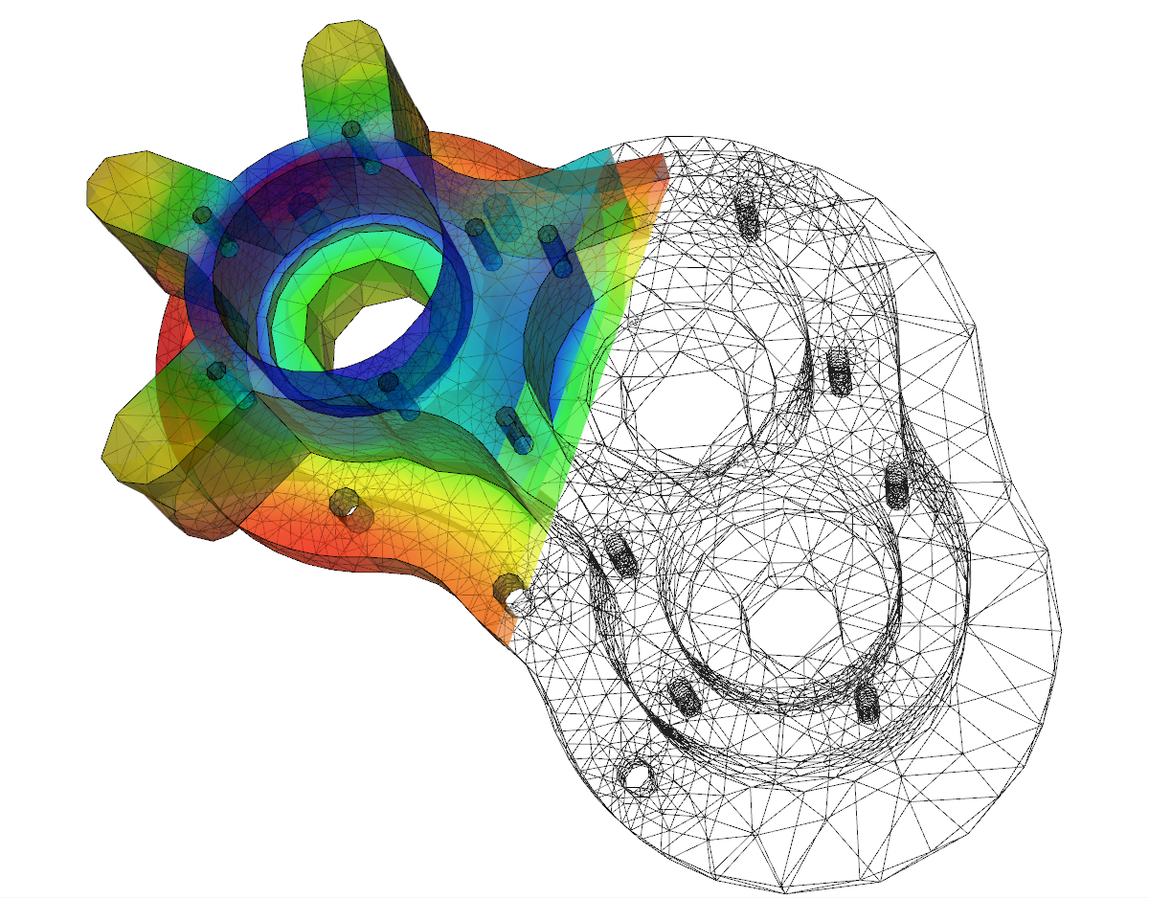
\includegraphics[width=0.55\textwidth]{chapters/chp6_pics/Elmer-pump-heatequation.png}
\caption{\textit{Visualizing the application of differential equations in finite element analysis (FEA), where partial differential equations (PDEs) model stress, strain, and deformation across complex geometries.}}
    \label{fig:fea_heat_equation}
\end{figure}

\subsection*{The Nature of Differential Equations}

\noindent A \textbf{differential equation} is an equation involving an unknown function and its derivatives. When we write:
\[
\frac{dy}{dx} = 2x
\]
we're expressing a relationship between an unknown function $y(x)$ and its derivative. The solution isn't just a number but a function—in this case, $y(x) = x^2 + C$. This represents a fundamental shift in our mathematical thinking: instead of finding values, we're finding functions that satisfy certain derivative relationships. \\

\noindent More formally, a differential equation can be written in the general form:
\[
F(x, y, y', y'', ..., y^{(n)}) = 0
\]
where $F$ is some function, $y$ is our unknown function, and $y^{(k)}$ represents the $k$th derivative of $y$. The order of a differential equation is the highest derivative that appears in it. For instance, $\frac{dy}{dx} = x^2$ is first-order, $\frac{d^2y}{dx^2} + \frac{dy}{dx} = \sin(x)$ is second-order, and $\frac{d^3y}{dx^3} - x\frac{dy}{dx} = e^x$ is third-order.

\noindent For differential equations with partial derivatives, we deal with functions of multiple variables, so the general form becomes:
\[
F(x_1, x_2, ..., x_n, u, \frac{\partial u}{\partial x_1}, \frac{\partial u}{\partial x_2}, ..., \frac{\partial^2 u}{\partial x_1^2}, \frac{\partial^2 u}{\partial x_1\partial x_2}, ...) = 0
\]
where $u = u(x_1, x_2, ..., x_n)$ is our unknown function of multiple variables, and $\frac{\partial u}{\partial x_i}$ represents partial derivatives with respect to the variable $x_i$. The order of a PDE is determined by the highest partial derivative that appears. For example:
\begin{itemize}
\item $\frac{\partial u}{\partial t} = \alpha\frac{\partial^2 u}{\partial x^2}$ (Heat equation) is second-order
\item $\frac{\partial^2 u}{\partial t^2} = c^2\frac{\partial^2 u}{\partial x^2}$ (Wave equation) is second-order
\item $\frac{\partial^2 u}{\partial x^2} + \frac{\partial^2 u}{\partial y^2} = 0$ (Laplace equation) is second-order
\end{itemize}

\subsubsection*{Origins and Formation}

\noindent Differential equations emerge naturally when we observe how quantities change in relation to each other. Consider a simple pendulum: its acceleration (second derivative of position) is proportional to its displacement, leading to:
\[
\frac{d^2\theta}{dt^2} = -\frac{g}{L}\sin(\theta)
\]
where $\theta$ is the angle from vertical, $g$ is gravitational acceleration, and $L$ is the pendulum length. How might we even begin to solve such an equation? Our calculus instincts suggest integration, but integrating both sides still leaves us with $\frac{d\theta}{dt}$ in terms of an integral of $\sin(\theta)$. This hints at the deeper complexity we'll encounter. \\

\noindent The process of forming differential equations often begins with physical insight. For instance, Newton's law of cooling states that the rate of temperature change is proportional to the temperature difference:
\[
\frac{dT}{dt} = -k(T - T_a)
\]
where $T$ is the object's temperature, $T_a$ is ambient temperature, and $k$ is a constant. Here we might have more success - notice how we could potentially separate variables with $T$ and $t$ on different sides. \\

\noindent Not all differential equations involve a single variable. Heat flow through a metal plate, as we saw, depends on position in both $x$ and $y$ directions and time $t$:
\[
\frac{\partial u}{\partial t} = \alpha\left(\frac{\partial^2 u}{\partial x^2} + \frac{\partial^2 u}{\partial y^2}\right)
\]
where $u(x,y,t)$ is temperature and $\alpha$ is thermal diffusivity. Such partial differential equations present entirely new challenges - now we're seeking functions of multiple variables! 

\exampleline
\begin{example}
A cup of hot coffee is sitting in a room of constant temperature 20°C. If the coffee's temperature drops from 90°C to 60°C in the first 10 minutes, model the coffee's temperature over time.
\begin{solution}
Let's think about how temperature changes:
\begin{enumerate}
\item First, let's understand what affects the rate of cooling:
\begin{itemize}
   \item The hotter the coffee is compared to the room, the faster it cools
   \item As the coffee gets closer to room temperature, cooling slows down
   \item The room stays at 20°C (we say it's the ambient temperature)
\end{itemize}
\item Let's translate this into mathematics:
\begin{itemize}
   \item Let $T(t)$ be the coffee's temperature at time $t$
   \item The rate of change is $\frac{dT}{dt}$
   \item The temperature difference from room temperature is $(T - 20)$
\end{itemize}
\item The rate of cooling is proportional to the temperature difference between the object and the surrounding environment. The constant in the differential equation must be negative to reflect that the object's temperature decreases over time when it is warmer than the surroundings. This yields the differential equation:
\[
\frac{dT}{dt} = -k(T - 20)
\]
\noindent This is actually known as Newton's Law of Cooling. We may find the constant $k$ using our initial conditions which will be discussed later.
\end{enumerate}

\end{solution}
\end{example}
\exampleline

\subsubsection*{Approaches to Solutions}

\noindent Solving differential equations requires a fundamentally different mindset from standard calculus. Consider first a seemingly simple ODE:
\[
\frac{dy}{dx} + y = e^x
\]
We seek a function $y(x)$ that, when substituted back, satisfies this relationship. But how? We could try guessing - since $e^x$ appears on the right, perhaps $y = Ce^x$ for some constant $C$? Or maybe we need a more systematic approach? \\

\noindent Some equations graciously yield to direct integration:
\[
\frac{dy}{dx} = x^2\sin(x)
\]
immediately suggests integrating both sides. But what about:
\[
\frac{\partial^2 u}{\partial x^2} = \frac{\partial^2 u}{\partial t^2}
\]
the famous wave equation? Integration seems less helpful here - we're dealing with partial derivatives in multiple variables. Perhaps we need a completely different strategy, like assuming solutions have a special form? \\

\noindent When analytical methods fail us, we might turn to numerical approximations. Consider discretizing our domain into small steps and approximating derivatives with finite differences:
\[
\frac{dy}{dx} \approx \frac{y(x + h) - y(x)}{h}
\]
This suggests iterative schemes that computers can implement. For PDEs, we might need to discretize in multiple dimensions, leading to systems of algebraic equations. \\

\noindent Sometimes, understanding behavior proves more valuable than finding exact solutions. For the logistic equation:
\[
\frac{dP}{dt} = rP\left(1 - \frac{P}{K}\right)
\]
we can identify equilibrium points by setting $\frac{dP}{dt} = 0$. But what about stability? How can we determine whether small perturbations grow or decay without an explicit solution? These questions lead us to qualitative theory - a powerful tool for understanding solution behavior even when exact formulas elude us. \\

\noindent We will systematically approach how to solve both ordinary and partial differential equations in the upcoming lectures.



\subsection*{Fundamental Classifications} \index{Differential Equations!Classifications}

\noindent Moving beyond basic definitions, differential equations naturally organize themselves into several fundamental categories. Each classification not only helps us understand the equation's nature but also suggests which solution methods might prove fruitful. \\

\noindent First and most fundamentally, we distinguish between ordinary and partial differential equations. An \textbf{ordinary differential equation (ODE)} \index{Ordinary Differential Equations} involves an unknown function of a single independent variable. For instance:
\[
\frac{d^2 y}{dx^2} + 3\frac{dy}{dx} + 2y = 0
\]
represents a second-order ODE. The term "ordinary" emphasizes that only ordinary derivatives appear, not partial derivatives. \\

\noindent In contrast, a \textbf{partial differential equation (PDE)} \index{Partial Differential Equations} involves an unknown function of several independent variables. The classic two-dimensional Laplace equation:
\[
\frac{\partial^2 u}{\partial x^2} + \frac{\partial^2 u}{\partial y^2} = 0
\]
appears across physics in steady-state heat conduction, electrostatics, and fluid flow. This distinction impacts not just complexity but determines which theoretical tools we can employ. \\

\noindent Another crucial distinction lies between linear and nonlinear equations. A \textbf{linear ODE of order n} \index{Linear Differential Equations} takes the form:
\[
a_n(x)\frac{d^n y}{dx^n} + a_{n-1}(x)\frac{d^{n-1}y}{dx^{n-1}} + \cdots + a_0(x)y = g(x)
\]
where $a_0, a_1, \dots, a_n, g$ are functions of $x$ alone. Linearity means $y$ and its derivatives appear to the first power, without multiplications between them and without nonlinear transformations like $\sin(y)$ or $y^2$. \\

\noindent A \textbf{nonlinear equation} \index{Nonlinear Differential Equations} violates these conditions. Terms like $(y')^2$, $y \cdot y'$, or $e^y$ indicate nonlinearity. While more challenging to solve, these equations often better capture physical reality, describing phenomena like turbulent flows or complex chemical reactions. \\

\noindent The \textbf{order} \index{Differential Equations!Order} of a differential equation is defined by its highest derivative. A third-order equation, for instance, contains terms up to $\frac{d^3y}{dx^3}$ but no higher. Higher-order equations commonly describe complex physical systems like beam deflection or wave propagation. \\

\noindent We further distinguish between homogeneous and non-homogeneous equations. A \textbf{homogeneous equation} \index{Homogeneous Differential Equations} of order $n$ has the form:
\[
a_n(x)y^{(n)} + a_{n-1}(x)y^{(n-1)} + \cdots + a_0(x)y = 0
\]
If instead the right side equals some non-zero function $g(x)$, we have a \textbf{non-homogeneous equation} \index{Non-homogeneous Differential Equations}. The homogeneous case describes free evolution, while non-homogeneous equations include external forcing. \\

\noindent Finally, for linear ODEs, we distinguish between constant and variable coefficients. In constant-coefficient equations:
\[
a_n\frac{d^n y}{dx^n} + a_{n-1}\frac{d^{n-1}y}{dx^{n-1}} + \cdots + a_0y = g(x)
\]
the coefficients $a_k$ are constants. Such equations often yield to standard solution methods. Variable-coefficient equations, where coefficients depend on $x$, typically demand more sophisticated approaches. \\

\noindent These classifications form the foundation for understanding differential equations. As we progress, we'll develop specific techniques for each type, but first recognizing an equation's category often suggests which approach might prove most fruitful.

\subsection*{Initial and Boundary Conditions} \index{Initial Conditions} \index{Boundary Conditions}

\noindent A crucial insight in differential equations is that a single equation typically has infinitely many solutions. Consider the simple equation:
\[
\frac{dy}{dx} = -2xy
\]
whose general solution we found to be $y = Ae^{-x^2}$. Each value of $A$ gives a different solution curve, collectively forming a family of solutions. \\

\begin{figure}[H]
\centering
\begin{tikzpicture}[scale=1.5]
    % Draw axes
    \draw[->] (-2,0) -- (2,0) node[right] {$x$};
    \draw[->] (0,-2) -- (0,2) node[above] {$y$};
    
    % Draw solution curves for different values of A
    \foreach \a in {-2,-1.5,-1,-0.5,0.5,1,1.5,2} {
        \draw[blue, domain=-2:2,samples=100] plot (\x,{\a*exp(-\x*\x)});
    }
    
    % Draw particular solution with A=1 in red
    \draw[red,thick, domain=-2:2,samples=100] plot (\x,{exp(-\x*\x)});
    
    % Add legend
    \begin{scope}[shift={(2.5,1.5)}]
        \draw[blue] (0,0) -- (0.5,0) node[right] {$y = Ae^{-x^2}$};
        \draw[red,thick] (0,-0.3) -- (0.5,-0.3) node[right] {$y = e^{-x^2}$};
        \draw[black,thin] (-0.1,0.2) rectangle (2,-0.5);
    \end{scope}
\end{tikzpicture}
\caption{\textit{Family of solutions to $\frac{dy}{dx} = -2xy$. The blue curves show different solutions for various values of $A$, while the red curve highlights the particular solution where $A=1$.}}
\label{fig:solution_family}
\end{figure}

\noindent To single out a particular solution from this family, we need additional information. This typically comes in two forms:
\begin{enumerate}

\item \textbf{Initial Conditions} \index{Initial Value Problem} specify the value of the unknown function (and possibly its derivatives) at a single point. For example, if we require:
\[
y(0) = 3
\]
this selects the unique solution curve passing through the point $(0,3)$. As we saw earlier, this leads to $A=3$ and the particular solution $y = 3e^{-x^2}$. For higher-order equations, we might need multiple conditions at the same point:
\[
\begin{cases} 
y(0) = 1 \\ 
y'(0) = 0 
\end{cases}
\]

\item \textbf{Boundary Conditions} \index{Boundary Value Problem} specify values at multiple points. For instance:
\[
y(0) = 0, \quad y(1) = 2
\]
requires our solution to pass through both $(0,0)$ and $(1,2)$. This type of condition often appears in physical problems like heat distribution or beam deflection where we know values at the endpoints of our domain.
\end{enumerate}

\noindent An equation together with sufficient conditions forms either an \textbf{Initial Value Problem (IVP)} or \textbf{Boundary Value Problem (BVP)}, depending on the type of conditions specified. The distinction is more than technical—the methods we use to solve these problems and even the nature of their solutions can differ dramatically. For instance:

\begin{enumerate}
   \item IVPs typically have unique solutions that can be ``evolved" forward from the initial condition
   \item BVPs might have multiple solutions, no solutions, or unique solutions depending on the boundary conditions
   \item Higher-order equations require correspondingly more conditions for uniqueness
\end{enumerate}

\noindent The geometric interpretation is illuminating: initial/boundary conditions effectively ``select" one curve from the infinite family of possible solutions. This idea of a family of solutions punctuated by particular solutions meeting specific conditions will recur throughout our study of differential equations, helping us understand both the general behavior of solutions and the role of additional conditions in selecting specific ones. Note, that the order of the equation must require that many conditions in order to fully produce a particular solution.

\exampleline
\begin{example}
Consider the ordinary differential equation:
\[
\frac{dy}{dx} = -2xy
\]
with initial condition $y(0) = 3$. Let's carefully examine how we might solve this equation.

\begin{solution}
Let's think about how to solve this step by step. We have a first order differential equation where we can separate all terms with $y$ on one side and all terms with $x$ on the other. \\

\noindent First, let's rearrange the equation to group $y$ terms and $x$ terms:
\[
\frac{dy}{y} = -2x\,dx
\]

\noindent Now we can integrate both sides. On the left, we recognize $\frac{dy}{y}$ as the derivative of $\ln|y|$:
\begin{align*}
\int \frac{dy}{y} &= \int -2x\,dx \\
\ln|y| &= -x^2 + C
\end{align*}

\noindent To solve for $y$, we exponentiate both sides:
\[
|y| = e^{-x^2 + C} = e^{-x^2}e^C = Ae^{-x^2}
\]
where $A = e^C$ is some positive constant. Since $A$ can be positive or negative (thanks to the absolute value), our general solution is:
\[
y = Ae^{-x^2}
\]

\noindent Now we can use our initial condition $y(0) = 3$ to find $A$:
\begin{align*}
3 &= Ae^{-0^2} \\
3 &= A \cdot 1 \\
A &= 3
\end{align*}

\noindent Therefore, our particular solution is:
\[
y = 3e^{-x^2}
\]
\end{solution}
\end{example}
\exampleline
\subsection*{Verification of Solutions} \index{Verification of Solutions}

\noindent Verifying solutions to differential equations is a critical step in ensuring the accuracy of our work. While finding solutions often requires creativity and problem-solving, verification is a systematic process that provides confidence in the correctness of the result. This process can be broken into clear steps for clarity and consistency. \\

\noindent First, we compute the necessary derivatives of the proposed solution. These derivatives are the building blocks we need to substitute back into the original differential equation. Next, by substituting the solution and its derivatives into the equation, we check whether the left-hand side equals the right-hand side. If this identity holds true, it confirms that the solution satisfies the differential equation itself. Finally, we verify any additional conditions, such as initial or boundary values, to ensure the solution fully satisfies all requirements of the problem. \\

\noindent Consider a simple example. To verify that $y(x) = x^2 + 1$ solves $\frac{dy}{dx} = 2x$:
\begin{align*}
\text{Given solution: } & y(x) = x^2 + 1 \\
\text{Compute derivative: } & \frac{dy}{dx} = 2x \\
\text{Original equation: } & \frac{dy}{dx} = 2x \\
\text{Therefore: } & 2x = 2x \quad \text{(Identity verified)}
\end{align*}

\noindent For higher-order equations, we must check more derivatives. Consider verifying that $y(x) = e^{2x}$ solves $\frac{d^2y}{dx^2} - 4y = 0$:
\begin{align*}
\text{Given: } & y = e^{2x} \\
\text{First derivative: } & \frac{dy}{dx} = 2e^{2x} \\
\text{Second derivative: } & \frac{d^2y}{dx^2} = 4e^{2x} \\
\text{Substitute: } & 4e^{2x} - 4(e^{2x}) = 0 \\
\text{Simplify: } & 0 = 0 \quad \text{(Identity verified)}
\end{align*}

\noindent For partial differential equations, we follow the same principle but must compute partial derivatives. To verify $u(x,t) = e^{-\pi^2t}\sin(\pi x)$ solves the heat equation $\frac{\partial u}{\partial t} = \frac{\partial^2 u}{\partial x^2}$:
\begin{align*}
\text{Given: } & u = e^{-\pi^2t}\sin(\pi x) \\
\text{Time derivative: } & \frac{\partial u}{\partial t} = -\pi^2e^{-\pi^2t}\sin(\pi x) \\
\text{Space derivative: } & \frac{\partial u}{\partial x} = \pi e^{-\pi^2t}\cos(\pi x) \\
\text{Second space derivative: } & \frac{\partial^2 u}{\partial x^2} = -\pi^2e^{-\pi^2t}\sin(\pi x) \\
\text{Original equation: } & \frac{\partial u}{\partial t} = \frac{\partial^2 u}{\partial x^2} \\
\text{Substitute: } & -\pi^2e^{-\pi^2t}\sin(\pi x) = -\pi^2e^{-\pi^2t}\sin(\pi x) \\
\text{Therefore: } & \text{Identity verified}
\end{align*}

\noindent Important considerations when verifying solutions:
\begin{enumerate}
   \item Check \textit{all} conditions - not just the differential equation but also initial/boundary conditions
   \item Pay attention to domains - where is the solution valid?
   \item Watch for hidden assumptions - are we dividing by zero anywhere?
   \item Use verification as a sanity check - does the solution make physical sense?
\end{enumerate}

\noindent Verification plays a crucial role in solving differential equations. It helps catch computational errors, validates the solution techniques, and builds confidence in our methods. Moreover, it fosters intuition about the behavior of solutions, enhancing our understanding of the problem. \\

\exampleline
\begin{example}
Verify that $y = x + \sum_{n=1}^{\infty} \frac{y^n}{n}$ is a solution to $y' = 1-\frac{1}{y}$. Discuss any insights about this solution.

\begin{solution}
Let's follow our verification steps:

\item Compute derivatives
  \begin{itemize}
     \item We have an implicit equation requiring implicit differentiation
     \item Start with: $y = x + \sum_{n=1}^{\infty} \frac{y^n}{n}$
     \item Differentiate both sides:
       \begin{align*}
       \frac{d}{dx}(y) &= \frac{d}{dx}\left(x + \sum_{n=1}^{\infty} \frac{y^n}{n}\right) \\
       y' &= 1 + \sum_{n=1}^{\infty} \frac{ny^{n-1}}{n}y' \\
       &= 1 + y'\sum_{n=1}^{\infty} y^{n-1}
       \end{align*}
  \end{itemize}

\item Manipulate to standard form
  \begin{itemize}
     \item Recognize $\sum_{n=1}^{\infty} y^{n-1}$ as geometric series $\frac{1}{1-y}$ for $|y| < 1$
     \item Therefore: $y' = 1 + y'\frac{1}{1-y}$
     \item Solve for $y'$:
       \begin{align*}
       y'\left(1 - \frac{1}{1-y}\right) &= 1 \\
       y'\left(\frac{-y}{1-y}\right) &= 1 \\
       y' &= 1 - \frac{1}{y}
       \end{align*}
  \end{itemize}

\item Additional insights
  \begin{itemize}
     \item The sum $\sum_{n=1}^{\infty} \frac{y^n}{n}$ is the Taylor series of $-\ln(1-y)$
     \item Solution can be written more compactly: $y = x - \ln(1-y)$
     \item Valid only for $|y| < 1$ due to series convergence
  \end{itemize}
\end{solution}
\end{example}
\exampleline

\newpage

\lecture{First-Order Ordinary Differential Equations} \index{First-Order ODEs}

\noindent Having established the fundamental nature and classification of differential equations, we now delve into our first systematic study of solution techniques for first-order ordinary differential equations. These equations, while seemingly simple in form, encompass a rich variety of mathematical structures and solution methods that form the foundation for understanding more complex differential equations. \\

\noindent A \textbf{first-order ordinary differential equation} can be written in the general form:
\[
F(x, y, y') = 0
\]
where $F$ is some function of the independent variable $x$, the dependent variable $y$, and its first derivative $y'$. More commonly, we encounter these equations in solved form:
\[
\frac{dy}{dx} = f(x,y)
\]
where $f(x,y)$ represents the relationship between the variables and the rate of change. \\

\noindent The designation ``first-order" refers to the highest derivative present in the equation - in this case, only the first derivative appears. This seemingly simple characteristic has profound implications. Unlike higher-order equations which may require multiple conditions to specify a unique solution, a first-order equation requires only a single initial condition of the form $y(x_0) = y_0$ to determine a unique solution (when one exists). \\

\noindent When studying first-order equations, we often encounter them in various standard forms, each suggesting its own solution strategy. For instance, when $f(x,y)$ can be written as a product of functions of $x$ and $y$ separately, we have a separable equation. When $f(x,y)$ is linear in $y$, we have a linear first-order equation. These special forms, which we will study in detail, provide scaffolding for understanding more general cases. \\

\noindent The existence and uniqueness of solutions to first-order equations is governed by the fundamental theorem for first-order ODEs: if $f(x,y)$ and $\frac{\partial f}{\partial y}$ are continuous in some rectangle containing an initial point $(x_0, y_0)$, then there exists a unique solution to the initial value problem in some interval containing $x_0$. This theorem provides theoretical foundation for our solution methods and helps us understand when and where we can expect solutions to exist.

\subsection*{Separation of Variables} \index{Separation of Variables}

\noindent The method of separation of variables represents our first and easiest systematic approach to solving differential equations. This technique applies when we can rewrite our equation in the form:
\[
\frac{dy}{dx} = f(x)g(y)
\]
where $f$ depends only on $x$ and $g$ depends only on $y$. The key insight is to rearrange terms so that all $y$-dependent terms are on one side and all $x$-dependent terms are on the other. This will always be your go to first visual check when trying to solve an ODE.\\

\noindent More formally, we rewrite the equation as:
\[
\frac{1}{g(y)}dy = f(x)dx
\]
This transformation allows us to integrate both sides independently:
\[
\int \frac{1}{g(y)}dy = \int f(x)dx + C
\]

\noindent The resulting equation implicitly defines $y$ as a function of $x$. In fortunate cases, we can solve explicitly for $y$, though often the solution remains in implicit form. This method's elegance lies in its reduction of a differential equation to algebraic manipulation and integration. This method obviously extends for cases of higher order derivatives which will be addressed later in this chapter.\\

\noindent Several theoretical considerations deserve attention:
\begin{enumerate}
    \item The method assumes $g(y) \neq 0$. Points where $g(y) = 0$ may yield additional solutions.
    \item The integration introduces a constant $C$, generating a family of solutions. Both integrations of $g$ and $f$ produce an arbitrary constant, but we can just combine them to form one arbitrary constant instead of two -- A fact that will be used frequently in the solving of DEs.
    \item Solutions may exist only on intervals where both $f$ and $g$ are continuous.
\end{enumerate}

\noindent We have already reasoned our way through one separable ODE in the last lecture. Let's try one that is not so obvious:

\exampleline
\begin{example}
Solve the differential equation:
\[
\frac{dy}{dx} = \frac{xy+3x+2y+6}{xy+x+y+1}
\]

\begin{solution}
Let's solve this step by step:
\begin{enumerate}
\item First, notice that both numerator and denominator can be factored through grouping:
   \begin{align*}
   xy+3x+2y+6 &= x(y+3)+2(y+3) \\
   &= (x+2)(y+3)
   \end{align*}
   And similarly:
   \begin{align*}
   xy+x+y+1 &= x(y+1)+1(y+1) \\
   &= (x+1)(y+1)
   \end{align*}

\item Our differential equation becomes:
   \[
   \frac{dy}{dx} = \frac{(x+2)(y+3)}{(x+1)(y+1)}
   \]

\item To separate variables, multiply both sides by $dx$ and rearrange:
   \[
   \frac{y+1}{y+3}\,dy = \frac{x+2}{x+1}\,dx
   \]

\item To integrate, first perform partial fractions on each side:
   \begin{align*}
   \frac{y+1}{y+3} &= 1 - \frac{2}{y+3} \\
   \frac{x+2}{x+1} &= 1 + \frac{1}{x+1}
   \end{align*}

\item Our equation becomes:
   \[
   \int \left(1 - \frac{2}{y+3}\right)dy = \int \left(1 + \frac{1}{x+1}\right)dx
   \]

\item Integrate both sides:
   \begin{align*}
   y - 2\ln|y+3| + C_1 &= x + \ln|x+1| + C_2
   \end{align*}

\item Combining constants, our general solution is:
   \[
   y - 2\ln|y+3| = x + \ln|x+1| + C, x \neq -1, y \neq -3
   \]
\end{enumerate}
\end{solution}
\end{example}
\exampleline


\subsection*{Linear First-Order Equations} \index{Linear First-Order ODEs}

\noindent A \textbf{linear first-order ODE} takes the standard form:
\[
\frac{dy}{dx} + P(x)y = Q(x)
\]
where $P(x)$ and $Q(x)$ are continuous functions. The linearity refers to the fact that $y$ and its derivative appear to the first power only, with no products between them and no nonlinear functions of $y$. When $Q(x) = 0$, we call the equation homogeneous; otherwise, it's non-homogeneous. This distinction plays a crucial role in both the theory and solution methods. \\

\noindent Any first-order linear equation can be written in this standard form through algebraic manipulation. For instance, equations like:
\[
\frac{dy}{dx} = ay + b \quad \text{or} \quad x\frac{dy}{dx} - 2y = x^3
\]
can be rewritten in standard form by collecting terms and dividing appropriately. This standardization is more than cosmetic—it reveals the underlying structure and suggests solution strategies. \\

\noindent The solution method involves an elegant technique called the \textbf{integrating factor} \index{Integrating Factor}. The key insight is that our equation almost looks like the product rule for derivatives (we're aiming for $(\mu y)' = \mu'y + \mu y')$, but not quite. If we could somehow make the left side into a perfect differential—that is, find a function $\mu(x)$ that when multiplied through makes the left side exactly the derivative of a product $\frac{d}{dx}[\mu(x)y]$—then we could solve by simple integration. With this motivation in mind, we multiply both sides by a carefully chosen function $\mu(x)$ that makes the left side the derivative of a product:
\[
\mu(x)\frac{dy}{dx} + \mu(x)P(x)y = \mu(x)Q(x)
\]

\noindent The magic of this method lies in choosing $\mu(x)$ to make the left side a perfect differential. The integrating factor $\mu(x)$ must satisfy:
\[
\frac{d}{dx}[\mu(x)y] = \mu(x)\frac{dy}{dx} + \mu'(x)y
\]
For this to equal our left side, we require:
\[
\mu'(x)y = \mu(x)P(x)y
\]
Therefore:
\[
\mu'(x) = \mu(x)P(x)
\]

\noindent This first-order separable equation for $\mu$ yields:
\[
\frac{d\mu}{\mu} = P(x)dx
\]
Integration gives us:
\[
\mu(x) = e^{\int P(x)dx}
\]

\noindent After multiplication by $\mu(x)$, our equation takes the elegant form:
\[
\frac{d}{dx}[\mu(x)y] = \mu(x)Q(x)
\]
Integration yields the general solution:
\[
y = \frac{1}{\mu(x)}\left[\int \mu(x)Q(x)dx + C\right]
\]

\noindent Several theoretical aspects deserve attention:

\begin{enumerate}
    \item The integrating factor is not unique—any constant multiple of $\mu(x)$ also works.
    \item The solution process naturally splits into finding a complementary function (solution to homogeneous equation) and a particular integral.
    \item The method always works when $P(x)$ and $Q(x)$ are continuous, making it one of our most reliable tools.
\end{enumerate}

\noindent The form of this solution reveals a fundamental principle: every linear first-order ODE can be solved through integration alone. This is not true for nonlinear equations, where we often need more sophisticated techniques. The solution also exhibits the superposition principle characteristic of linear equations: the general solution is the sum of a particular solution and the general solution to the homogeneous equation. \\

\noindent When $Q(x) = 0$ (homogeneous case), our solution simplifies to:
\[
y = \frac{C}{\mu(x)} = Ce^{-\int P(x)dx}
\]
This form clearly shows how the integrating factor ``undoes" the effect of the coefficient $P(x)$. The exponential form of this solution appears frequently in applications, modeling phenomena like radioactive decay and temperature cooling.

\exampleline
\begin{example}
Solve the differential equation:
\[
x^2\frac{dy}{dx} - 3xy = x^3\cos(x) + 2x^2y
\]

\begin{solution}
\begin{enumerate}
\item First, we need to rearrange into standard form $\frac{dy}{dx} + P(x)y = Q(x)$:
   \begin{align*}
   x^2\frac{dy}{dx} - 3xy &= x^3\cos(x) + 2x^2y \\
   x^2\frac{dy}{dx} - 3xy - 2x^2y &= x^3\cos(x) \\
   x^2\frac{dy}{dx} - x y(3+2x) &= x^3\cos(x)
   \end{align*}
   
   Divide throughout by $x^2$ (note: this restricts our domain to $x \neq 0$):
   \[
   \frac{dy}{dx} - \frac{y(3+2x)}{x} = x\cos(x)
   \]
   
   Therefore:
   \[
   \frac{dy}{dx} + \frac{y(-3-2x)}{x} = x\cos(x)
   \]

\item Now we have standard form with:
   \[
   P(x) = -\frac{3+2x}{x} \quad \text{and} \quad Q(x) = x\cos(x)
   \]

\item Find the integrating factor $\mu(x) = e^{\int P(x)dx}$:
   \begin{align*}
   \mu(x) &= e^{\int -\frac{3+2x}{x}dx} \\
   &= e^{\int (-\frac{3}{x}-2)dx} \\
   &= e^{-3\ln|x|-2x} \\
   &= e^{-2x}x^{-3}
   \end{align*}

\item Multiply the equation by $\mu(x)$:
   \[
   e^{-2x}x^{-3}\frac{dy}{dx} + e^{-2x}x^{-3}\cdot\frac{-3-2x}{x}y = e^{-2x}x^{-3}\cdot x\cos(x)
   \]
   
   This is equivalent to:
   \[
   \frac{d}{dx}(e^{-2x}x^{-3}y) = e^{-2x}x^{-2}\cos(x)
   \]

\item Integrate both sides:
   \[
   e^{-2x}x^{-3}y = \int e^{-2x}x^{-2}\cos(x)dx + C
   \]

\item Therefore:
   \[
   y = x^3e^{2x}\left[\int e^{-2x}x^{-2}\cos(x)dx + C\right]
   \]
\noindent Sometimes, we must leave the integral in the solution if it is too hard to evaluate -- and that's perfectly fine!
\end{enumerate}

\end{solution}
\end{example}
\exampleline

\subsection*{Exact Differential Equations} \index{Exact Differential Equations}

\noindent An equation of the form:
\[
M(x,y)dx + N(x,y)dy = 0
\]
is called \textbf{exact} if there exists a function $\psi(x,y)$, called the potential function, such that:
\[
d\psi = M(x,y)dx + N(x,y)dy
\]
This implies:
\[
\frac{\partial \psi}{\partial x} = M(x,y) \quad \text{and} \quad \frac{\partial \psi}{\partial y} = N(x,y)
\]

\noindent The fundamental theorem of calculus for line integrals tells us this occurs precisely when:
\[
\frac{\partial M}{\partial y} = \frac{\partial N}{\partial x}
\]
This condition is both necessary and sufficient for exactness, providing a straightforward test before attempting to find a solution. When an equation is exact, its solution is implicit in the form:

\[
\psi(x,y) = C
\]

\noindent There are two methods for finding the potential function $\psi(x,y)$: \\

\noindent \textbf{Method 1: Integration with respect to $x$, then find $h(y)$} \\
\begin{enumerate}
    \item Integrate $M(x,y)$ with respect to $x$, treating $y$ as constant:
    \[
    \psi(x,y) = \int M(x,y)dx + h(y)
    \]
    where $h(y)$ is an arbitrary function of $y$ alone.
    
    \item To find $h(y)$, differentiate $\psi$ with respect to $y$:
    \[
    \frac{\partial \psi}{\partial y} = \frac{\partial}{\partial y}\left[\int M(x,y)dx\right] + h'(y)
    \]
    
    \item Since $\frac{\partial \psi}{\partial y} = N(x,y)$, we have:
    \[
    \frac{\partial}{\partial y}\left[\int M(x,y)dx\right] + h'(y) = N(x,y)
    \]
    
    \item Solve for $h'(y)$:
    \[
    h'(y) = N(x,y) - \frac{\partial}{\partial y}\left[\int M(x,y)dx\right]
    \]
    
    \item Integrate to find $h(y)$:
    \[
    h(y) = \int h'(y)dy
    \]
\end{enumerate}

\noindent \textbf{Method 2: Integration with respect to $y$, then find $g(x)$} \\
\begin{enumerate}
    \item Integrate $N(x,y)$ with respect to $y$, treating $x$ as constant:
    \[
    \psi(x,y) = \int N(x,y)dy + g(x)
    \]
    where $g(x)$ is an arbitrary function of $x$ alone.
    
    \item To find $g(x)$, differentiate $\psi$ with respect to $x$:
    \[
    \frac{\partial \psi}{\partial x} = \frac{\partial}{\partial x}\left[\int N(x,y)dy\right] + g'(x)
    \]
    
    \item Since $\frac{\partial \psi}{\partial x} = M(x,y)$, we have:
    \[
    \frac{\partial}{\partial x}\left[\int N(x,y)dy\right] + g'(x) = M(x,y)
    \]
    
    \item Solve for $g'(x)$:
    \[
    g'(x) = M(x,y) - \frac{\partial}{\partial x}\left[\int N(x,y)dy\right]
    \]
    
    \item Integrate to find $g(x)$:
    \[
    g(x) = \int g'(x)dx
    \]
\end{enumerate}

\noindent \textbf{Important Observations:}
\begin{enumerate}
    \item Both methods must yield the same potential function $\psi(x,y)$ (up to a constant) if the equation is exact.
    
    \item The exactness condition $\frac{\partial M}{\partial y} = \frac{\partial N}{\partial x}$ ensures that either method works and gives consistent results.
    
    \item When finding $h(y)$ or $g(x)$, the resulting expression must be independent of $x$ or $y$ respectively. If not, the equation is not exact.
    
    \item The verification process is crucial: after finding $\psi(x,y)$, we should check that both $\frac{\partial \psi}{\partial x} = M(x,y)$ and $\frac{\partial \psi}{\partial y} = N(x,y)$ are satisfied.
    
    \item The constant of integration can be omitted when finding $h(y)$ or $g(x)$ since it will be absorbed into the final constant $C$ in the general solution $\psi(x,y) = C$.
\end{enumerate}

\noindent The geometric interpretation of exact differential equations is profound: the solution curves are level curves of the potential function $\psi(x,y)$, and $M(x,y)dx + N(x,y)dy = 0$ represents the condition that motion along a solution curve maintains a constant value of $\psi$.

\exampleline
\begin{example}
Show that the differential equation:
\[
(2xy + y^2)\,dx + (x^2 + 2xy)\,dy = 0
\]
is exact, and solve it using both methods.

\begin{solution}
Let's solve this systematically:

\begin{enumerate}
\item First, let's verify that the equation is exact by checking if $\frac{\partial M}{\partial y} = \frac{\partial N}{\partial x}$:
   \begin{align*}
   M(x,y) &= 2xy + y^2 \quad \implies \frac{\partial M}{\partial y} = 2x + 2y \\
   N(x,y) &= x^2 + 2xy \quad \implies \frac{\partial N}{\partial x} = 2x + 2y
   \end{align*}
   Since $\frac{\partial M}{\partial y} = \frac{\partial N}{\partial x}$, the equation is exact.

\item \textbf{Method 1:} Integrate $M(x,y)$ with respect to $x$
   \begin{align*}
   \psi(x,y) &= \int M(x,y)\,dx + h(y) \\
   &= \int (2xy + y^2)\,dx + h(y) \\
   &= x^2y + xy^2 + h(y)
   \end{align*}
   
   Now find $h(y)$ by comparing $\frac{\partial \psi}{\partial y}$ with $N(x,y)$:
   \begin{align*}
   \frac{\partial \psi}{\partial y} &= x^2 + 2xy + h'(y) = N(x,y) = x^2 + 2xy \\
   \therefore h'(y) &= 0 \\
   \therefore h(y) &= C_1
   \end{align*}
   
   Thus, by Method 1:
   \[
   \psi(x,y) = x^2y + xy^2 + C_1
   \]

\item \textbf{Method 2:} Integrate $N(x,y)$ with respect to $y$
   \begin{align*}
   \psi(x,y) &= \int N(x,y)\,dy + g(x) \\
   &= \int (x^2 + 2xy)\,dy + g(x) \\
   &= x^2y + xy^2 + g(x)
   \end{align*}
   
   Now find $g(x)$ by comparing $\frac{\partial \psi}{\partial x}$ with $M(x,y)$:
   \begin{align*}
   \frac{\partial \psi}{\partial x} &= 2xy + y^2 + g'(x) = M(x,y) = 2xy + y^2 \\
   \therefore g'(x) &= 0 \\
   \therefore g(x) &= C_2
   \end{align*}
   
   Thus, by Method 2:
   \[
   \psi(x,y) = x^2y + xy^2 + C_2
   \]

\item The general solution is:
   \[
   \psi(x,y) = x^2y + xy^2 = C
   \]
   where $C = -C_1 = -C_2$ is an arbitrary constant.
\end{enumerate}

\noindent Several important observations:
\begin{itemize}
   \item Both methods yielded the same potential function $\psi(x,y)$ (up to a constant)
   \item We can verify our solution by checking that $\frac{\partial \psi}{\partial x} = M(x,y)$ and $\frac{\partial \psi}{\partial y} = N(x,y)$
   \item The solution represents a family of level curves of $\psi(x,y)$
   \item The integrating constants $C_1$ and $C_2$ from each method combine into a single constant $C$ in the final solution
\item The equation \(x^2y + xy^2 = C\) can be rewritten to form a quadratic in \(y\). Dividing by \(x\):
\[
y^2 + xy - \frac{C}{x} = 0.
\]
Using the quadratic formula, we solve for \(y\):
\[
y = \frac{-x \pm \sqrt{x^2 + \frac{4C}{x}}}{2}.
\]
Thus, the explicit solutions for \(y\) are:
\[
y = \frac{-x + \sqrt{x^2 + \frac{4C}{x}}}{2} \quad \text{and} \quad y = \frac{-x - \sqrt{x^2 + \frac{4C}{x}}}{2}.
\]


\end{itemize}
\end{solution}
\end{example}
\exampleline

\subsection*{Bernoulli Differential Equations} \index{Bernoulli Differential Equations}

\noindent A \textbf{Bernoulli differential equation} takes the form:
\[
\frac{dy}{dx} + P(x)y = Q(x)y^n
\]
where $n$ is any real number except 0 or 1, and $P(x)$ and $Q(x)$ are continuous functions. When $n = 0$, the equation reduces to a linear equation, and when $n = 1$, the equation is already linear. Therefore, these cases are excluded from our consideration. \\

\noindent The brilliance of Bernoulli's insight was recognizing that a clever substitution could transform this nonlinear equation into a linear one. The key transformation is:
\[
v = y^{1-n}
\]

\noindent Let's see how this transformation works. First, differentiate $v$ with respect to $x$ using the chain rule:
\[
\frac{dv}{dx} = (1-n)y^{-n}\frac{dy}{dx}
\]

\noindent From our original equation:
\[
\frac{dy}{dx} = -P(x)y + Q(x)y^n
\]

\noindent Substituting this into our expression for $\frac{dv}{dx}$:
\begin{align*}
\frac{dv}{dx} &= (1-n)y^{-n}(-P(x)y + Q(x)y^n) \\
&= (1-n)[-P(x)y^{1-n} + Q(x)y^{n-n}] \\
&= (1-n)[-P(x)v + Q(x)]
\end{align*}

\noindent This transforms our equation into the linear form:
\[
\frac{dv}{dx} + (1-n)P(x)v = (1-n)Q(x)
\]

\noindent This is a linear first-order equation in $v$ which we can solve using the integrating factor method. The integrating factor is:
\[
\mu(x) = e^{(1-n)\int P(x)dx}
\]

\noindent Following the standard procedure for linear equations, the general solution for $v$ is:
\[
v = e^{-(1-n)\int P(x)dx}\left[\int (1-n)Q(x)e^{(1-n)\int P(x)dx}dx + C\right]
\]

\noindent Substituting back $v = y^{1-n}$, we obtain the general solution for the Bernoulli equation:
\[
y = \left\{e^{-(1-n)\int P(x)dx}\left[\int (1-n)Q(x)e^{(1-n)\int P(x)dx}dx + C\right]\right\}^{\frac{1}{1-n}}
\]

\noindent Several important observations about Bernoulli equations:
\begin{enumerate}
    \item The transformation $v = y^{1-n}$ is valid only when $y \neq 0$. The zero solution may need to be checked separately.
    
    \item The exponent $n$ plays a crucial role in determining the behavior of solutions. Different values of $n$ can lead to dramatically different solution behaviors.
    
    \item When $n < 0$, solutions may have vertical asymptotes. When $n > 1$, solutions may have horizontal asymptotes.
    
    \item The integrating factor method used after transformation highlights the deep connection between linear and nonlinear differential equations.
    
    \item Bernoulli equations often arise in applications where quantities grow or decay with power-law behavior, such as in population dynamics and chemical reactions.
\end{enumerate}

\noindent The Bernoulli equation serves as a bridge between linear and nonlinear theory. While it's nonlinear in its original form, its amenability to transformation into a linear equation makes it one of the few nonlinear equations for which we can write down a general solution formula. This makes it an excellent introduction to the study of nonlinear differential equations.

\exampleline
\begin{example}
Solve the Bernoulli equation \( y' + y = y^2 \).

\begin{solution}
Here \( P(x) = 1 \), \( Q(x) = 1 \), and \( n = 2 \). We substitute \( v = y^{1-n} = y^{-1} = 1/y \), so \( v' = -y^{-2}y' \). Dividing the original equation by \( y^2 \):
\[ y^{-2}y' + y^{-1} = 1 \quad \Rightarrow \quad -v' + v = 1 \quad \Rightarrow \quad v' - v = -1. \]
This is a linear first-order equation with integrating factor \( \mu = e^{-x} \):
\[ \frac{d}{dx}(ve^{-x}) = -e^{-x} \quad \Rightarrow \quad ve^{-x} = e^{-x} + C \quad \Rightarrow \quad v = 1 + Ce^x. \]
Substituting back \( v = 1/y \):
\[ y = \frac{1}{1 + Ce^x}. \]
\end{solution}
\end{example}
\exampleline

\subsection*{A Word on Existence and Uniqueness} \index{Existence and Uniqueness Theorems}

\noindent When studying differential equations, two fundamental questions arise: does a solution exist, and if so, is it unique? These questions are not merely theoretical—they inform us whether our solution methods will be fruitful and whether we can trust that we've found all possible solutions. \\

\noindent For a first-order differential equation in the form:
\[
\frac{dy}{dx} = f(x,y), \quad y(x_0) = y_0
\]
the \textbf{Existence Theorem} \index{Existence Theorem} states that a solution exists if $f(x,y)$ is continuous in some rectangle containing the initial point $(x_0, y_0)$. This solution may not be valid for all $x$, but it exists in some interval containing $x_0$. \\

\noindent The \textbf{Uniqueness Theorem} \index{Uniqueness Theorem} adds that this solution is unique if $\frac{\partial f}{\partial y}$ is also continuous in this rectangle. Together, these conditions are known as the \textbf{Existence and Uniqueness Theorem}. \\

\noindent The geometric interpretation is illuminating. Consider the slope field of the differential equation:
\begin{itemize}
    \item Continuity of $f(x,y)$ ensures the slopes vary smoothly—no sudden jumps or breaks
    \item Continuity of $\frac{\partial f}{\partial y}$ ensures the slopes change smoothly as we move vertically—preventing solution curves from crossing
\end{itemize}

\noindent Several important scenarios can violate these conditions:
\begin{enumerate}
    \item When $f(x,y)$ has a discontinuity, solutions might not exist. For example:
    \[
    \frac{dy}{dx} = \frac{1}{x}, \quad y(0) = 0
    \]
    has no solution through $(0,0)$ due to division by zero.
    
    \item When $\frac{\partial f}{\partial y}$ is discontinuous, multiple solutions might exist. Consider:
    \[
    \frac{dy}{dx} = |y|^{\frac{1}{3}}
    \]
    Through $(0,0)$, both $y = 0$ and $y = \pm\left(\frac{2x}{3}\right)^{\frac{3}{2}}$ are solutions.
\end{enumerate}

\noindent For higher-order equations:
\[
y^{(n)} = f(x, y, y', ..., y^{(n-1)})
\]
we can convert to a system of first-order equations and apply similar principles. The key conditions become:
\begin{itemize}
    \item $f$ must be continuous in all variables
    \item $\frac{\partial f}{\partial y^{(k)}}$ must be continuous for $k = 0, 1, ..., n-1$
\end{itemize}

\noindent These theorems provide powerful guarantees:
\begin{itemize}
    \item When conditions are met, numerical methods will converge to the unique solution
    \item Local existence ensures our solution methods are meaningful
    \item Uniqueness validates our practice of finding general solutions with arbitrary constants
\end{itemize}

\noindent However, these theorems have limitations:
\begin{enumerate}
    \item They only guarantee local existence—solutions might blow up in finite time
    \item They don't tell us how to find the solution
    \item They don't specify the size of the interval where the solution exists
\end{enumerate}

\noindent Understanding existence and uniqueness helps us approach differential equations with confidence, knowing when our methods will yield meaningful results and when we need to exercise caution in our analysis. These theorems form the theoretical foundation that supports all our practical solution techniques. \\

\noindent While we have focused on ordinary differential equations, existence and uniqueness theory extends crucially to partial differential equations. In PDEs, the questions become significantly more complex due to the multiple independent variables involved. For example, the well-posedness of a PDE problem requires not only existence and uniqueness but also continuous dependence on initial/boundary conditions. Classical PDEs like the heat equation, wave equation, and Laplace equation each have their own existence and uniqueness theorems with specific requirements on domains, boundary conditions, and solution regularity. The celebrated Cauchy-Kowalevski theorem provides existence and uniqueness for analytic solutions of certain PDEs, though its applicability is limited. These considerations become central when studying PDEs in more advanced courses.
\newpage

\lecture{Higher-Order Ordinary Differential Equations I} \index{Higher-Order ODEs}

\noindent Of course we cannot stop with analyzing functions with a single order derivative, thus we now venture into the rich territory of higher-order differential equations. These equations, containing derivatives of order two or greater, model a vast array of physical phenomena from the simple harmonic oscillator to complex structural vibrations, from gravitational interactions to quantum mechanical systems. Their study reveals deeper mathematical structures and requires more sophisticated solution techniques.

\subsection*{Fundamental Concepts} \index{Higher-Order ODEs!Fundamentals}

\noindent An \textbf{nth-order differential equation} is an equation containing derivatives up to order $n$. In its most general form, it can be written as:
\[
F(x, y, y', y'', ..., y^{(n)}) = 0
\]
or when solved for the highest derivative:
\[
y^{(n)} = f(x, y, y', y'', ..., y^{(n-1)})
\]
where $f$ is some function of $x$, $y$, and derivatives of $y$ up to order $n-1$. \\

\noindent A general \textbf{linear nth-order differential equation} takes the special form:
\[
a_n(x)\frac{d^ny}{dx^n} + a_{n-1}(x)\frac{d^{n-1}y}{dx^{n-1}} + \cdots + a_1(x)\frac{dy}{dx} + a_0(x)y = g(x)
\]
where $a_n(x), a_{n-1}(x), \ldots, a_0(x)$ are continuous functions with $a_n(x) \neq 0$, and $g(x)$ is also continuous. When $g(x) = 0$, we call the equation homogeneous; otherwise, it's non-homogeneous. \\

\noindent A particularly important case arises when all coefficients are constants:
\[
a_n\frac{d^ny}{dx^n} + a_{n-1}\frac{d^{n-1}y}{dx^{n-1}} + \cdots + a_1\frac{dy}{dx} + a_0y = g(x)
\]

\noindent For both linear and nonlinear equations, the order of the equation determines how many additional conditions we need for a unique solution. For an $n$th-order equation, we need $n$ conditions of the form:
\[
y(x_0) = y_0, \quad y'(x_0) = y_1, \quad \ldots, \quad y^{(n-1)}(x_0) = y_{n-1}
\]

\noindent This requirement of n initial conditions is not arbitrary but follows from the fundamental theory of differential equations. Each condition serves to determine one of the arbitrary constants that arise in the general solution. \\

\noindent The existence and uniqueness theorem for nth-order equations states that if $f$ and its partial derivatives with respect to $y, y', ..., y^{(n-1)}$ are continuous in some region containing the initial point, then there exists a unique solution in some interval containing $x_0$. This holds for both linear and nonlinear equations. \\

\noindent A fundamental difference between linear and nonlinear equations lies in how solutions can be combined. For linear equations, any linear combination of solutions is again a solution (the superposition principle). This property does not hold for nonlinear equations, making their analysis generally more challenging.

\subsection*{The Principle of Superposition} \index{Higher-Order ODEs!Superposition}

\noindent One of the most powerful tools in solving linear differential equations is the principle of superposition, which states:

\begin{enumerate}
    \item If $y_1(x)$ and $y_2(x)$ are solutions to the homogeneous equation, then $c_1y_1(x) + c_2y_2(x)$ is also a solution for any constants $c_1, c_2$.
    
    \item If $y_h(x)$ is a solution to the homogeneous equation and $y_p(x)$ is a particular solution to the non-homogeneous equation, then $y_h(x) + y_p(x)$ is a general solution to the non-homogeneous equation.
\end{enumerate}

\noindent Let's prove both parts. Consider the linear differential equation:
\[
a_n(x)\frac{d^ny}{dx^n} + a_{n-1}(x)\frac{d^{n-1}y}{dx^{n-1}} + \cdots + a_1(x)\frac{dy}{dx} + a_0(x)y = g(x)
\]

\noindent \textbf{Part 1 (Homogeneous Case):} \\
Let $y_1$ and $y_2$ be solutions to the homogeneous equation. Then:
\[
a_n(x)\frac{d^ny_1}{dx^n} + \cdots + a_0(x)y_1 = 0
\]
\[
a_n(x)\frac{d^ny_2}{dx^n} + \cdots + a_0(x)y_2 = 0
\]

\noindent For any constants $c_1, c_2$, consider $y = c_1y_1 + c_2y_2$. Note that:
\[
\frac{d^k}{dx^k}(c_1y_1 + c_2y_2) = c_1\frac{d^ky_1}{dx^k} + c_2\frac{d^ky_2}{dx^k}
\]
for any $k$. Therefore:
\begin{align*}
&a_n(x)\frac{d^n}{dx^n}(c_1y_1 + c_2y_2) + \cdots + a_0(x)(c_1y_1 + c_2y_2) \\
&= c_1[a_n(x)\frac{d^ny_1}{dx^n} + \cdots + a_0(x)y_1] + c_2[a_n(x)\frac{d^ny_2}{dx^n} + \cdots + a_0(x)y_2] \\
&= c_1(0) + c_2(0) = 0
\end{align*}

\noindent \textbf{Part 2 (Non-homogeneous Case):} \\
Let $y_h$ be a solution to the homogeneous equation and $y_p$ a particular solution. Then:
\[
a_n(x)\frac{d^ny_h}{dx^n} + \cdots + a_0(x)y_h = 0
\]
\[
a_n(x)\frac{d^ny_p}{dx^n} + \cdots + a_0(x)y_p = g(x)
\]

\noindent For $y = y_h + y_p$, using the linearity of differentiation:
\begin{align*}
&a_n(x)\frac{d^n}{dx^n}(y_h + y_p) + \cdots + a_0(x)(y_h + y_p) \\
&= [a_n(x)\frac{d^ny_h}{dx^n} + \cdots + a_0(x)y_h] + [a_n(x)\frac{d^ny_p}{dx^n} + \cdots + a_0(x)y_p] \\
&= 0 + g(x) = g(x)
\end{align*}

\noindent This principle allows us to build complex solutions from simpler ones and suggests our general strategy: first find the complementary function (general solution to homogeneous equation), then find a particular solution. The proof reveals why this principle works only for linear equations - we crucially used the fact that derivatives of sums are sums of derivatives, and that we can factor out constants.

\subsection*{Second-Order Linear Equations} \index{Higher-Order ODEs!Second Order}

\noindent Second-order differential equations arise naturally in many physical contexts and serve as the foundation for understanding higher-order equations. In their most general form, they appear as:
\[
p(x)\frac{d^2y}{dx^2} + q(x)\frac{dy}{dx} + r(x)y = g(x)
\]
where $p(x)$, $q(x)$, and $r(x)$ are continuous functions with $p(x) \neq 0$, and $g(x)$ is also continuous. When $g(x) = 0$, we have a homogeneous equation; otherwise, it's non-homogeneous. \\

\noindent A particularly important special case occurs when the coefficients are constants:
\[
a\frac{d^2y}{dx^2} + b\frac{dy}{dx} + cy = g(x)
\]
where $a$, $b$, and $c$ are constants with $a \neq 0$. This form appears frequently in applications such as:
\begin{itemize}
    \item Simple harmonic motion
    \item Forced oscillations
    \item RLC circuits
    \item Beam deflection
\end{itemize}

\noindent When the equation is autonomous (no explicit $x$ dependence) and homogeneous:
\[
a\frac{d^2y}{dx^2} + b\frac{dy}{dx} + cy = 0
\]
we can develop particularly powerful solution methods based on characteristic equations (which we will cover next). But first, a crucial concept in the study of second-order equations is that of linear independence. Two solutions $y_1(x)$ and $y_2(x)$ are said to be \textbf{linearly independent} \index{Linear Independence} on an interval $I$ if no nontrivial linear combination vanishes on that interval. That is, if:
\[
c_1y_1(x) + c_2y_2(x) = 0
\]
for all $x$ in $I$ implies $c_1 = c_2 = 0$. \\

\noindent Linear independence can be tested using the \textbf{Wronskian} \index{Wronskian}, defined as:
\[
W(y_1, y_2)(x) = y_1y_2' - y_2y_1'
\]
If $W(y_1, y_2)(x) \neq 0$ at any point in an interval, then $y_1$ and $y_2$ are linearly independent there. When we have two linearly independent solutions to the homogeneous equation, any solution can be written as their linear combination:
\[
y = c_1y_1(x) + c_2y_2(x)
\]
where $c_1$ and $c_2$ are determined by initial conditions.

\subsubsection*{The Characteristic Equation Method} \index{Characteristic Equation Method}

\noindent For homogeneous constant-coefficient equations:
\[
ay'' + by' + cy = 0
\]
we seek solutions of the form $y = e^{rx}$. Substituting this ansatz:
\[
ar^2e^{rx} + bre^{rx} + ce^{rx} = 0
\]
\[
e^{rx}(ar^2 + br + c) = 0
\]

\noindent Since $e^{rx} \neq 0$, we obtain the characteristic equation:
\[
ar^2 + br + c = 0
\]

\noindent The nature of the roots determines the form of our solution:

\begin{enumerate}
    \item Distinct real roots $r_1, r_2$:
    \[
    y = c_1e^{r_1x} + c_2e^{r_2x}
    \]
    
    \item Repeated real root $r_1$:
    \[
    y = c_1e^{r_1x} + c_2xe^{r_1x}
    \]
    
    \item Complex conjugate roots $\alpha \pm i\beta$:
    \[
    y = e^{\alpha x}(c_1\cos(\beta x) + c_2\sin(\beta x))
    \]
\end{enumerate}

\noindent This method extends naturally to higher orders. For an nth-order equation:
\[
a_ny^{(n)} + a_{n-1}y^{(n-1)} + \cdots + a_1y' + a_0y = 0
\]
the characteristic equation becomes:
\[
a_nr^n + a_{n-1}r^{n-1} + \cdots + a_1r + a_0 = 0
\]

\noindent The Fundamental Theorem of Algebra ensures n complex roots (counting multiplicity), leading to the following solution patterns:
\begin{itemize}
    \item For a real root $r$ of multiplicity $k$: $e^{rx}, xe^{rx}, x^2e^{rx}, \ldots, x^{k-1}e^{rx}$
    \item For complex conjugate pairs $\alpha \pm i\beta$: $e^{\alpha x}\cos(\beta x), e^{\alpha x}\sin(\beta x)$
    \item For repeated complex pairs: multiply by increasing powers of $x$
\end{itemize}

\subsection*{Method of Undetermined Coefficients} \index{Method of Undetermined Coefficients}

\noindent The method of undetermined coefficients provides a systematic approach to finding particular solutions of non-homogeneous linear differential equations with constant coefficients. The process begins with finding the complementary function and then addresses the forcing term. \\

\noindent Consider the non-homogeneous equation:
\[
ay'' + by' + cy = g(x)
\]

\noindent The complete solution will have the form:
\[
y = y_h + y_p
\]
where $y_h$ is the general solution to the homogeneous equation and $y_p$ is a particular solution. \\

\noindent \textbf{Step 1: Find the Complementary Function:} First, solve the homogeneous equation:
\[
ay'' + by' + cy = 0
\]
using the characteristic equation method. This gives $y_h$, which contains arbitrary constants. \\

\noindent \textbf{Step 2: Address the Forcing Function:} For the non-homogeneous part, we use superposition when $g(x)$ is a sum of terms:
\[
g(x) = g_1(x) + g_2(x) + \cdots + g_n(x)
\]
This allows us to solve simpler equations:
\[
ay'' + by' + cy = g_k(x)
\]
for each $k$, and then add the solutions: $y_p = y_{p1} + y_{p2} + \cdots + y_{pn}$. \\

\noindent For each type of forcing term, we have specific trial solutions:

\begin{enumerate}
    \item For polynomials $g(x) = P_n(x)$ of degree $n$:
       \[
       y_p = A_nx^n + A_{n-1}x^{n-1} + \cdots + A_1x + A_0
       \]
       
    \item For exponentials $g(x) = e^{ax}$:
       \[
       y_p = Ae^{ax}
       \]
       
    \item For trigonometric terms $g(x) = \cos(bx)$ or $\sin(bx)$:
       \[
       y_p = A\cos(bx) + B\sin(bx)
       \]
       
    \item For products $g(x) = x^ne^{ax}$:
       \[
       y_p = (A_nx^n + A_{n-1}x^{n-1} + \cdots + A_0)e^{ax}
       \]
       
    \item For combined trigonometric-exponential terms:
       \[
       g(x) = e^{ax}(P\cos(bx) + Q\sin(bx)) \implies y_p = e^{ax}(R\cos(bx) + S\sin(bx))
       \]
\end{enumerate}

\noindent \textbf{The Resonance Case:} If any term in the trial solution is also a solution to the homogeneous equation, we must modify our guess. This happens when:
\begin{itemize}
    \item The forcing function matches a term in $y_h$
    \item The characteristic equation has a root related to the forcing function
\end{itemize}

\noindent In such cases, multiply the trial solution by $x^k$ where $k$ is the minimum power needed for linear independence. For example:
\begin{itemize}
    \item If $e^{rx}$ is both a forcing term and in $y_h$, try $y_p = Axe^{rx}$
    \item If it's a double root, try $y_p = Ax^2e^{rx}$
\end{itemize}

\noindent Consider:
\[
y'' - y = 3e^x + 2\cos(x) + x^2
\]
We break this into three equations:
\begin{align*}
y'' - y &= 3e^x && \text{(exponential term)} \\
y'' - y &= 2\cos(x) && \text{(trigonometric term)} \\
y'' - y &= x^2 && \text{(polynomial term)}
\end{align*}

\noindent For each equation:
\begin{enumerate}
    \item First find $y_h$ from $y'' - y = 0$: 
       \[
       y_h = c_1e^x + c_2e^{-x}
       \]
       
    \item Then find each $y_{pk}$ using appropriate trial solutions
    
    \item Combine all solutions: 
       \[
       y = y_h + y_{p1} + y_{p2} + y_{p3}
       \]
\end{enumerate}

\noindent This systematic approach, combined with superposition, allows us to solve a wide range of non-homogeneous equations efficiently. The key is recognizing that:
\begin{enumerate}
    \item The homogeneous solution must be found first
    \item Complex forcing functions can be broken down
    \item Each piece can be solved independently
    \item The sum of all solutions gives the general solution
    \item Resonance cases require special attention
\end{enumerate}

\exampleline
\begin{example}
Solve the differential equation:
\[
y'' - 4y' + 4y = 2x + 3e^{2x} + 4\sin(x)
\]

\begin{solution}
We'll solve via superposition, handling the homogeneous part and then each non-homogeneous term separately.

\begin{enumerate}
\item \textbf{Homogeneous solution:} Solve
   \[
   y'' - 4y' + 4y = 0.
   \]
   \[
   \text{Characteristic eq.: } r^2 - 4r + 4 = 0 \quad \Longrightarrow \quad (r-2)^2 = 0 \quad \Longrightarrow \quad r = 2 \ (\text{double root}).
   \]
   \[
   y_h = c_1 e^{2x} + c_2 x e^{2x}.
   \]

\item \textbf{Non-homogeneous terms:}
   \[
   g_1(x) = 2x, 
   \quad
   g_2(x) = 3e^{2x},
   \quad
   g_3(x) = 4\sin(x).
   \]
   We find particular solutions for each and sum them.

\item \textbf{Particular solution for $g_1(x) = 2x$:}

   Try \(y_{p1} = Ax + B.\)

   \[
   y_{p1}' = A,\quad
   y_{p1}'' = 0.
   \]
   Substitute into \(y'' - 4y' + 4y\):
   \[
   0 - 4A + 4(Ax + B) = 2x.
   \]
   \[
   4Ax + 4B - 4A = 2x.
   \]
   Matching coefficients:
   \[
   4A = 2 \ \Longrightarrow\ A = \tfrac12,
   \qquad
   4B - 4A = 0 \ \Longrightarrow\ B = \tfrac12.
   \]
   \[
   y_{p1} = \tfrac12 x + \tfrac12.
   \]

\item \textbf{Particular solution for $g_2(x) = 3e^{2x}$:}

   Since \(e^{2x}\) is part of the homogeneous solution (double root at \(r=2\)), try
   \[
   y_{p2} = A x^2 e^{2x}.
   \]
   Compute derivatives (correctly applying the product rule):
   \[
   y_{p2}' = \frac{d}{dx}\bigl(Ax^2 e^{2x}\bigr)
           = A e^{2x}\bigl(2x^2 + 2x\bigr),
   \]
   \[
   y_{p2}'' = \frac{d}{dx}\bigl(A e^{2x}(2x^2 + 2x)\bigr)
            = 2A e^{2x}\bigl(2x^2 + 4x + 1\bigr).
   \]
   Substitute into \(y'' - 4y' + 4y\):
   \[
   \bigl(2A(2x^2 + 4x + 1)e^{2x}\bigr)
   - 4\bigl(A e^{2x}(2x^2 + 2x)\bigr)
   + 4\bigl(Ax^2 e^{2x}\bigr)
   = 3e^{2x}.
   \]
   After simplification, the expression collapses to \(2A\,e^{2x}\). So
   \[
   2A\,e^{2x} = 3\,e^{2x}
   \ \Longrightarrow\
   A = \frac{3}{2}.
   \]
   \[
   y_{p2} = \tfrac{3}{2} x^2 e^{2x}.
   \]

\item \textbf{Particular solution for $g_3(x) = 4\sin(x)$:}

   Try \(y_{p3} = A\cos(x) + B\sin(x).\)

   \[
   y_{p3}' = -A\sin(x) + B\cos(x), \quad
   y_{p3}'' = -A\cos(x) - B\sin(x).
   \]
   Substitute into \(y'' - 4y' + 4y\):
   \[
   (-A\cos x - B\sin x)
   \;-\;4(-A\sin x + B\cos x)
   \;+\;4(A\cos x + B\sin x).
   \]
   Collecting terms:
   \[
   \cos(x):\quad (-A) + (-4B) + (4A) = 3A - 4B,
   \]
   \[
   \sin(x):\quad (-B) + (4A) + (4B) = 4A + 3B.
   \]
   We want
   \[
   (3A - 4B)\cos(x) + (4A + 3B)\sin(x) = 4\sin(x).
   \]
   Hence
   \[
   3A - 4B = 0, 
   \quad
   4A + 3B = 4.
   \]
   Solve:
   \[
   3A = 4B \ \Longrightarrow\ A = \frac{4B}{3},
   \]
   \[
   4\Bigl(\tfrac{4B}{3}\Bigr) + 3B = 4 \ \Longrightarrow\ \tfrac{16B}{3} + 3B = 4 
   \ \Longrightarrow\ \tfrac{25B}{3} = 4 
   \ \Longrightarrow\ B = \tfrac{12}{25}, \quad A = \tfrac{16}{25}.
   \]
   \[
   y_{p3} = \frac{16}{25}\cos(x) + \frac{12}{25}\sin(x).
   \]

\item \textbf{Combine all parts for the general solution:}
   \[
   y = y_h + y_{p1} + y_{p2} + y_{p3}
     = c_1 e^{2x}
       + c_2 x e^{2x}
       + \tfrac{1}{2}x 
       + \tfrac{1}{2}
       + \tfrac{3}{2} x^2 e^{2x}
       + \frac{16}{25}\cos(x)
       + \frac{12}{25}\sin(x).
   \]
\end{enumerate}

\noindent This demonstrates how to handle each term independently and then superimpose results into one final solution.
\end{solution}
\end{example}
\exampleline
\begin{example}
Consider the fifth-order homogeneous linear differential equation with constant coefficients:
\[
y^{(5)} - 9y^{(4)} + 32y^{(3)} - 56y'' + 47y' - 15y = 0
\]

\begin{solution}
Let's solve this systematically:

\begin{enumerate}
\item Form the characteristic equation by replacing $y^{(n)}$ with $r^n$:
   \[
   r^5 - 9r^4 + 32r^3 - 56r^2 + 47r - 15 = 0
   \]

\item Factor this polynomial. By inspection or using algebraic methods, we find:
   \begin{align*}
   &r = 1 \text{ (double root)} \\
   &r = 3 \text{ (single root)} \\
   &r = 2 \pm i \text{ (complex conjugate pair)}
   \end{align*}
   
   Therefore our polynomial factors as:
   \[
   (r - 1)^2(r - 3)(r^2 - 4r + 5) = 0
   \]
   where $r^2 - 4r + 5 = (r - (2+i))(r - (2-i))$

\item Generate solutions based on each root type:
   \begin{itemize}
      \item For $r = 1$ (double root): 
         \[
         y_1 = e^x \text{ and } y_2 = xe^x
         \]
      
      \item For $r = 3$ (single root):
         \[
         y_3 = e^{3x}
         \]
      
      \item For $r = 2 \pm i$ (complex conjugate pair):
         \[
         y_4 = e^{2x}\cos(x) \text{ and } y_5 = e^{2x}\sin(x)
         \]
   \end{itemize}

\item Write the general solution as a linear combination:
   \[
   y = c_1e^x + c_2xe^x + c_3e^{3x} + e^{2x}(c_4\cos(x) + c_5\sin(x))
   \]
\end{enumerate}

\noindent Several important observations:
\begin{itemize}
   \item The double root at $r = 1$ contributes two terms: $e^x$ and $xe^x$
   \item The complex conjugate pair provides oscillatory behavior modulated by $e^{2x}$
   \item The number of arbitrary constants (5) matches the order of the equation
   \item Each term corresponds directly to a root or root pair of the characteristic equation
\end{itemize}
\end{solution}
\end{example}
\exampleline

\newpage
\lecture{Higher-Order Ordinary Differential Equations II} \index{Higher-Order ODEs}

\subsubsection*{Variation of Parameters} \index{Variation of Parameters}

\noindent
The \emph{method of undetermined coefficients} leverages structured guesses for $y_p$ (a particular solution) when the non-homogeneous term $g(x)$ has a familiar form (e.g.\ polynomials, exponentials, sines/cosines, or products thereof). However, for more complicated or ``weird'' source functions $g(x)$, such guesses may not be obvious or practical. In such cases, \emph{variation of parameters} provides a more general and powerful procedure that works \emph{without} depending on the form of $g(x)$. \\

\noindent
Consider the general second-order ODE:
\[
y'' + p(x)\,y' + q(x)\,y \;=\; g(x),
\]
where $p(x)$ and $q(x)$ are coefficient functions of $x$. Suppose we have already solved the associated \emph{homogeneous} equation,
\[
y'' + p(x)\,y' + q(x)\,y \;=\; 0,
\]
and found two linearly independent solutions, $y_1(x)$ and $y_2(x)$. Variation of parameters seeks a particular solution of the form
\[
y_p(x) \;=\; u_1(x)\,y_1(x) \;+\; u_2(x)\,y_2(x),
\]
where $u_1(x)$ and $u_2(x)$ are unknown functions to be determined. To find $u_1(x)$ and $u_2(x)$, we impose the conditions
\[
u_1'(x)\,y_1(x) \;+\; u_2'(x)\,y_2(x) \;=\; 0,
\]
\[
u_1'(x)\,y_1'(x) \;+\; u_2'(x)\,y_2'(x) \;=\; g(x),
\]
which simplify the algebra upon substituting $y_p(x)$ into the original differential equation. By solving this system for $u_1'(x)$ and $u_2'(x)$, we obtain:
\[
u_1'(x) \;=\; -\,\frac{y_2(x)\,g(x)}{W(x)},
\quad
u_2'(x) \;=\; \;\;\frac{y_1(x)\,g(x)}{W(x)},
\]
where
\[
W(x) \;=\; y_1(x)\,y_2'(x) - y_2(x)\,y_1'(x)
\]
is the \emph{Wronskian} of $y_1$ and $y_2$. The functions $u_1(x)$ and $u_2(x)$ then follow by integrating $u_1'$ and $u_2'$:
\[
u_1(x) \;=\; -\int \frac{y_2(x)\,g(x)}{W(x)}\,dx,
\qquad
u_2(x) \;=\; \int \frac{y_1(x)\,g(x)}{W(x)}\,dx.
\]

\noindent
Substituting $u_1(x)$ and $u_2(x)$ back into $y_p(x)$ provides a particular solution that, when combined with the homogeneous solution, yields the complete general solution to
\[
y'' + p(x)\,y' + q(x)\,y = g(x).
\]

\noindent
\textbf{More general cases:} This method scales naturally to higher-order ODEs. For the $n$th-order linear differential equation
\[
y^{(n)} + p_{n-1}(x)\,y^{(n-1)} + \cdots + p_0(x)\,y \;=\; g(x),
\]
one starts with $n$ linearly independent homogeneous solutions $y_1(x), \ldots, y_n(x)$ and proposes
\[
y_p(x) \;=\; u_1(x)\,y_1(x) + \cdots + u_n(x)\,y_n(x).
\]
The corresponding variation of parameters system ensures each $u_i(x)$ is determined consistently. This makes variation of parameters \emph{much more powerful} than undetermined coefficients, because it does not rely on recognizing special forms of $g(x)$. \\

\noindent
In summary, whenever the non-homogeneous term $g(x)$ does not match standard patterns for undetermined coefficients (or is simply too cumbersome to guess effectively), variation of parameters offers a systematic procedure for finding a particular solution, leveraging the homogeneous solution and the Wronskian.

\exampleline
\begin{example}
Solve the non-homogeneous ODE via Variation of Parameters:
\[
y'' \;+\; y \;=\; \tan(x).
\]

\begin{solution}
\begin{enumerate}
\item \textbf{Write the homogeneous equation.}

   The associated homogeneous ODE is
   \[
   y'' + y = 0.
   \]
   Its characteristic equation is
   \[
   r^2 + 1 = 0
   \;\Longrightarrow\;
   r = \pm\,i.
   \]
   Therefore, the general homogeneous solution is
   \[
   y_h(x)
   \;=\;
   C_1 \cos(x) \;+\; C_2 \sin(x).
   \]

\item \textbf{Set up Variation of Parameters for the non-homogeneous part.}

   We aim to find a \emph{particular} solution of the form
   \[
   y_p(x)
   \;=\;
   u_1(x)\,\cos(x) \;+\; u_2(x)\,\sin(x),
   \]
   where \(u_1(x)\) and \(u_2(x)\) are unknown functions.

\item \textbf{Identify the Wronskian and the standard formulas.}

   For two linearly independent solutions \(y_1(x) = \cos(x)\) and \(y_2(x) = \sin(x)\), their Wronskian is
   \[
   W(x)
   \;=\;
   \begin{vmatrix}
   y_1 & y_2 \\
   y_1' & y_2'
   \end{vmatrix}
   \;=\;
   \begin{vmatrix}
   \cos(x) & \sin(x) \\
   -\sin(x) & \cos(x)
   \end{vmatrix}
   \;=\;
   \cos^2(x) + \sin^2(x)
   \;=\;
   1.
   \]
   Variation of parameters (for a second-order ODE of the form \(y'' + p(x)\,y' + q(x)\,y = g(x)\)) gives:
   \[
   u_1'(x)
   \;=\;
   -\,\frac{y_2(x)\,g(x)}{W(x)},
   \qquad
   u_2'(x)
   \;=\;
   \frac{y_1(x)\,g(x)}{W(x)}.
   \]
   Here, \(g(x) = \tan(x)\), \(y_1(x) = \cos(x)\), \(y_2(x) = \sin(x)\), and \(W(x) = 1\).

\item \textbf{Find \(u_1'(x)\) and \(u_2'(x)\).}

   \[
   u_1'(x)
   \;=\;
   -\,\sin(x)\,\tan(x)
   \;=\;
   -\sin(x)\,\frac{\sin(x)}{\cos(x)}
   \;=\;
   -\frac{\sin^2(x)}{\cos(x)},
   \]
   \[
   u_2'(x)
   \;=\;
   \cos(x)\,\tan(x)
   \;=\;
   \cos(x)\,\frac{\sin(x)}{\cos(x)}
   \;=\;
   \sin(x).
   \]

\item \textbf{Integrate to find \(u_1(x)\) and \(u_2(x)\).}

   \[
   u_1(x)
   \;=\;
   \int
   u_1'(x)\,dx
   \;=\;
   \int
   \Bigl(-\frac{\sin^2(x)}{\cos(x)}\Bigr)\,dx
   \;=\;
   -\,\int \frac{\sin^2(x)}{\cos(x)}\,dx.
   \]
   Observe:
   \[
   \int \frac{\sin^2(x)}{\cos(x)}\,dx
   =
   \int \frac{1 - \cos^2(x)}{\cos(x)}\,dx
   =
   \int \sec(x)\,dx
   \;-\;
   \int \cos(x)\,dx.
   \]
   We know \(\int \sec(x)\,dx = \ln\bigl|\sec(x) + \tan(x)\bigr|\), and \(\int \cos(x)\,dx = \sin(x)\). Hence,
   \[
   \int \frac{\sin^2(x)}{\cos(x)}\,dx
   =
   \ln\bigl|\sec(x) + \tan(x)\bigr|
   \;-\;
   \sin(x).
   \]
   Thus,
   \[
   u_1(x)
   =
   -\Bigl[\ln\bigl|\sec(x) + \tan(x)\bigr| - \sin(x)\Bigr]
   =
   -\,\ln\bigl|\sec(x) + \tan(x)\bigr|
   \;+\;
   \sin(x).
   \]
   Meanwhile,
   \[
   u_2(x)
   \;=\;
   \int
   u_2'(x)\,dx
   \;=\;
   \int \sin(x)\,dx
   \;=\;
   -\,\cos(x).
   \]

\item \textbf{Write the particular solution.}

   We now have for $y_p(x)$:
   \[
   u_1(x)\cos(x) \;+\; u_2(x)\sin(x)
   \;=\;
   \bigl[\sin(x) - \ln|\sec(x) + \tan(x)|\bigr]\cos(x)
   -\cos(x)\sin(x).
   \]
   Notice that
   \(\sin(x)\cos(x)\;-\;\cos(x)\sin(x) = 0\).
   So the expression simplifies to:
   \[
   y_p(x)
   =
   -\,\cos(x)\,\ln\bigl|\sec(x) + \tan(x)\bigr|.
   \]

\item \textbf{Combine with the homogeneous solution for the general solution.}

   The full solution is
   \[
   y(x)
   \;=\;
   y_h(x) \;+\; y_p(x)
   \;=\;
   C_1\,\cos(x)
   \;+\;
   C_2\,\sin(x)
   \;-\;
   \cos(x)\,\ln\bigl|\sec(x) + \tan(x)\bigr|.
   \]
   where $C_1, C_2$ are arbitrary constants.
\end{enumerate}

\noindent This example illustrates how variation of parameters yields a particular solution even when standard guessing (undetermined coefficients) is not straightforward. By leveraging known homogeneous solutions and the Wronskian, we solve for functions $u_1(x)$ and $u_2(x)$ in a systematic way, regardless of the complexity of $\tan(x)$.
\end{solution}
\end{example}
\exampleline


\newpage

\lecture{Higher-Order Ordinary Differential Equations III} \index{Higher-Order ODEs}

And now after spending lots of time and effort learning very specific techniques, we will now introduce a method that will blast half of those out of the water. Transform methods are exceptionally powerful tools in solving ordinary differential equations (ODEs). Laplace Transforms convert differential equations into algebraic equations, simplifying the solution process. \\

\noindent These methods allow us to handle complex boundary conditions, discontinuities, and impulsive forcing functions with remarkable ease. By transforming an ODE into the frequency domain, the operations of differentiation and integration become multiplication and division, respectively, making the equations much more tractable. This approach not only simplifies the solution of linear ODEs but also provides insights into the behavior of physical systems, making transform methods indispensable in engineering, physics, and applied mathematics.

\subsection*{Introduction to Laplace Transforms} \index{Laplace Transform}

\noindent
The key idea behind the Laplace transform is to convert differential and integral operations in the time domain into algebraic operations in the complex frequency domain. This conversion often simplifies the process of solving differential equations by transforming them into algebraic equations, which are generally easier to manipulate and solve. \\

\noindent
Formally, the Laplace transform establishes a one-to-one correspondence between functions in the time domain and functions in the complex frequency domain, subject to certain conditions of existence. This correspondence allows us to solve problems in whichever domain is most convenient and then transform the solution back to the original domain. \\

\noindent For a function \(f(t)\) defined for \(t \geq 0\), the Laplace transform \(F(s)\) is defined as:
\[
F(s) \;=\; \mathcal{L}\{f(t)\} \;=\; \int_{0}^{\infty} e^{-s t}\,f(t)\,\mathrm{d}t,
\]
where \(s = \sigma + i\omega\) is a complex variable. The real part \(\sigma\) is called the attenuation, and the imaginary part \(\omega\) is called the angular frequency. The integral in the definition converges if \(f(t)\) is of exponential order, meaning there exist constants \(M > 0\), \(a\), and \(T\) such that \(\lvert f(t)\rvert \leq M e^{a t}\) for all \(t > T\). In this case, the integral converges for all \(s\) with \(\mathrm{Re}(s) > a\). \\

\noindent Laplace transforms offer several significant advantages in solving differential equations and analyzing linear systems:
\begin{enumerate}
\item \textbf{Differential to Algebraic Conversion:}
The Laplace transform converts an nth-order linear differential equation:
\[
a_n\frac{d^n y}{dt^n} + a_{n-1}\frac{d^{n-1} y}{dt^{n-1}} + \cdots + a_0 y = f(t)
\]
into a simpler algebraic equation:
\[
(a_n s^n + a_{n-1} s^{n-1} + \cdots + a_0)Y(s) = F(s) + \text{(initial conditions)}
\]

\item \textbf{Handling Discontinuous Functions:}
The transform elegantly handles discontinuous inputs through simple expressions:
\[
\mathcal{L}\{u(t)\} = \tfrac{1}{s}, \quad \mathcal{L}\{\delta(t)\} = 1
\]

\item \textbf{Initial Conditions:}
Initial conditions emerge naturally in the transformed derivatives:
\[
\mathcal{L}\{f'(t)\} = sF(s) - f(0), \quad \mathcal{L}\{f''(t)\} = s^2F(s) - sf(0) - f'(0)
\]

\item \textbf{Linear Time-Invariant Systems:}
The transform converts complex convolution operations:
\[
y(t) = \int_{0}^{t} h(\tau)x(t - \tau)\mathrm{d}\tau
\]
into simple multiplication:
\[
Y(s) = H(s)X(s)
\]
where H(s) represents the system's transfer function.
\end{enumerate}

\subsubsection*{Properties of Laplace Transforms}

The following properties form the core mathematical framework for applying Laplace transforms to differential equations and system analysis:

\begin{enumerate}
\item \textbf{Linearity:}
\[
\mathcal{L}\{a f(t) + b g(t)\} = a\,\mathcal{L}\{f(t)\} + b\,\mathcal{L}\{g(t)\}
\]
This fundamental property enables decomposition of complex functions into simpler elements.

\item \textbf{First Derivative:}
\[
\mathcal{L}\{f'(t)\} = s\,F(s) - f(0)
\]
Converts time-domain differentiation into s-domain multiplication.

\item \textbf{Higher-Order Derivatives:}
\[
\mathcal{L}\{f^{(n)}(t)\} = s^n F(s) - s^{n-1} f(0) - s^{n-2} f'(0) - \cdots - f^{(n-1)}(0)
\]
Extends the derivative property to nth-order derivatives.

\item \textbf{Integration:}
\[
\mathcal{L}\Bigl\{\int_{0}^{t} f(\tau)\,\mathrm{d}\tau\Bigr\} = \frac{1}{s}\,F(s)
\]
Transforms time-domain integration into s-domain division.

\item \textbf{Frequency Shifting:}
\[
\mathcal{L}\{e^{a t} \, f(t)\} = F(s - a)
\]
Handles exponential factors in time domain.

\item \textbf{Time Shifting:}
\[
\mathcal{L}\{f(t-a) \, u(t-a)\} = e^{-a s}\,F(s)
\]
Addresses delayed functions in time domain.

\item \textbf{Scaling:}
\[
\mathcal{L}\{f(a t)\} = \frac{1}{a}\,F\Bigl(\frac{s}{a}\Bigr)
\]
Relates time scaling to frequency scaling.

\item \textbf{Convolution:}
\[
\mathcal{L}\{f(t) * g(t)\} = F(s)\,G(s)
\]
Transforms time-domain convolution to s-domain multiplication.
\end{enumerate}

\noindent
The following comprehensive table presents common transform pairs essential for solving both initial value problems and boundary value problems. When solving differential equations, we first transform the equation using these pairs, solve the resulting algebraic equation in the $s$-domain, and then use these same pairs in reverse to find our time-domain solution.

{
\renewcommand{\arraystretch}{2}
\begin{table}[H]
\centering
\caption{\textit{Common Laplace Transform Pairs.}}
\label{table:laplace_transforms}
\begin{tabular}{|c|c||c|c|}
\hline
\(f(t)\) & \(\mathcal{L}\{f(t)\}\) & \(f(t)\) & \(\mathcal{L}\{f(t)\}\) \\ \hline
\(1\) & \(\dfrac{1}{s}\) & \(t\sin(at)\) & \(\dfrac{2as}{(s^2+a^2)^2}\) \\ \hline
\(t\) & \(\dfrac{1}{s^2}\) & \(t\cos(at)\) & \(\dfrac{s^2-a^2}{(s^2+a^2)^2}\) \\ \hline
\(t^n\) & \(\dfrac{n!}{s^{n+1}}\) & \(t^ne^{at}\) & \(\dfrac{n!}{(s-a)^{n+1}}\) \\ \hline
\(e^{at}\) & \(\dfrac{1}{s-a}\) & \(e^{at}\sin(bt)\) & \(\dfrac{b}{(s-a)^2+b^2}\) \\ \hline
\(\sin(at)\) & \(\dfrac{a}{s^2+a^2}\) & \(e^{at}\cos(bt)\) & \(\dfrac{s-a}{(s-a)^2+b^2}\) \\ \hline
\(\cos(at)\) & \(\dfrac{s}{s^2+a^2}\) & \(u(t-c)\) & \(\dfrac{e^{-cs}}{s}\) \\ \hline
\(\sinh(at)\) & \(\dfrac{a}{s^2-a^2}\) & \(\delta(t-c)\) & \(e^{-cs}\) \\ \hline
\(\cosh(at)\) & \(\dfrac{s}{s^2-a^2}\) & \(e^{at}f(t)\) & \(F(s-a)\) \\ \hline
\(te^{at}\) & \(\dfrac{1}{(s-a)^2}\) & \(\displaystyle\int_{0}^t\! f(\tau)g(t\!-\!\tau)\,d\tau\) & \(F(s)G(s)\) \\ \hline
\(\dfrac{\sin(at)}{t}\) & \(\tan^{-1}\!\left(\dfrac{a}{s}\right)\) & \(J_0(at)\) & \(\dfrac{1}{\sqrt{s^2+a^2}}\) \\ \hline
\end{tabular}

\medskip
\textit{General property:} $\mathcal{L}\{t^n f(t)\} = (-1)^n \dfrac{d^n}{ds^n} F(s)$
\end{table}
}
\subsubsection*{Steps for Solving ODEs Using Laplace Transforms}

To solve a linear ODE using Laplace transforms, we follow a systematic approach that transforms our problem into algebraic form and back:

\begin{enumerate}
\item \textbf{Forward Transform:} Take the Laplace transform of both sides of the ODE using Table \ref{table:laplace_transforms} and the properties of derivatives:
  \begin{itemize}
  \item \(\mathcal{L}\{y'\} = sY(s) - y(0)\)
  \item \(\mathcal{L}\{y''\} = s^2Y(s) - sy(0) - y'(0)\)
  \end{itemize}

\item \textbf{Algebraic Manipulation:} Solve the resulting algebraic equation for \(Y(s)\), typically obtaining a rational function:
  \[Y(s) = \frac{P(s)}{Q(s)}\]
  where \(P(s)\) and \(Q(s)\) are polynomials in \(s\).

\item \textbf{Partial Fraction Decomposition:} Just like in a standard Calculus II class, we break the rational function into simpler terms:
  \[\frac{P(s)}{Q(s)} = \frac{A}{s-a} + \frac{Bs + C}{s^2 + ps + q} + \cdots\]

\item \textbf{Inverse Transform:} Convert back to the time domain using Table \ref{table:laplace_transforms} in reverse.
\end{enumerate}

\subsubsection*{Inverse Laplace Transform Strategy}

While the inverse transform has a formal definition via complex integration:
\[
f(t) = \mathcal{L}^{-1}\{F(s)\} = \frac{1}{2\pi i} \int_{c - i \infty}^{\,c + i \infty} e^{s t}\,F(s)\,\mathrm{d}s,
\]
in practice, we use Table \ref{table:laplace_transforms} systematically:

\begin{enumerate}
\item \textbf{Pattern Recognition:} Look for standard forms in Table \ref{table:laplace_transforms}:
  \begin{itemize}
  \item \(\frac{1}{s-a} \rightarrow e^{at}\)
  \item \(\frac{s}{s^2 + a^2} \rightarrow \cos(at)\)
  \item \(\frac{a}{s^2 + a^2} \rightarrow \sin(at)\)
  \end{itemize}

\item \textbf{Linear Combination:} Use the linearity property:
  \[\mathcal{L}^{-1}\{aF(s) + bG(s)\} = af(t) + bg(t)\]

\item \textbf{Complex Terms:} For terms not directly in the table:
  \begin{itemize}
  \item Use shifting properties
  \item Apply derivative or integral properties
  \item Combine simpler known transforms
  \end{itemize}
\end{enumerate}

\exampleline
\begin{example}
Find the inverse Laplace transform of:
\[
F(s) = \frac{3}{s^2 + 4}
\]

\begin{solution}
\begin{enumerate}
\item First, analyze the form of $F(s)$:
   \begin{itemize}
      \item The denominator is a quadratic: $s^2 + 4 = s^2 + (2)^2$
      \item There is no $s$ term in the numerator
      \item The coefficient in front is 3
   \end{itemize}

\item Express $F(s)$ in standard form:
   \[
   F(s) = 3 \cdot \frac{1}{s^2 + (2)^2}
   \]
   This matches the form $\frac{1}{s^2 + a^2}$ with $a = 2$

\item Recall from our transform table that:
   \[
   \mathcal{L}^{-1}\left\{\frac{1}{s^2 + a^2}\right\} = \frac{1}{a}\sin(at)
   \]

\item Apply this result using the linearity property:
   \begin{align*}
   \mathcal{L}^{-1}\{F(s)\} &= \mathcal{L}^{-1}\left\{3 \cdot \frac{1}{s^2 + 4}\right\} \\
   &= 3 \cdot \mathcal{L}^{-1}\left\{\frac{1}{s^2 + 4}\right\} \\
   &= 3 \cdot \frac{1}{2}\sin(2t) \\
   &= \frac{3}{2}\sin(2t)
   \end{align*}
\end{enumerate}

\end{solution}
\end{example}
\exampleline

\noindent Now let's put everything we have learned together to tackle solving an ODE with Laplace Transforms. Note, that up till now, this is the most robust method of solving ODEs. However, beware that this is computationally tedious to work out and one small error can make you have a completely wrong solution. It is up to you to weigh which method you use to tackle ODEs. Typically, the more complicated source functions, the better Laplace Transforms are to solve the corresponding ODE.


\exampleline
\begin{example}
Solve the initial-value problem via Laplace transforms:
\[
y'' + 4y = \sin(2t), 
\quad y(0) = 0, 
\quad y'(0) = 0.
\]

\begin{solution}
\begin{enumerate}
\item \textbf{Take the Laplace transform of both sides:}

   Recall:
   \[
   \mathcal{L}\{y''\}(s) 
   = s^2Y(s) - s\,y(0) - y'(0), 
   \]
   and
   \[
   \mathcal{L}\{\sin(2t)\}(s) 
   = \frac{2}{s^2 + 4}.
   \]
   Given the initial conditions $y(0) = 0$ and $y'(0) = 0$, we have:
   \[
   \mathcal{L}\{y''\}(s) = s^2 Y(s).
   \]
   Therefore, applying the Laplace transform to the ODE gives:
   \[
   s^2 Y(s) + 4Y(s) 
   = \frac{2}{s^2 + 4}.
   \]

\item \textbf{Factor and solve for $Y(s)$:}

   \[
   (s^2 + 4)Y(s) 
   = \frac{2}{s^2 + 4} 
   \quad \Longrightarrow \quad
   Y(s) = \frac{2}{(s^2 + 4)^2}.
   \]

\item \textbf{Find the inverse Laplace transform of $Y(s)$:}

   We use the known result:
   \[
   \mathcal{L}^{-1}\left\{
      \frac{1}{(s^2 + a^2)^2}
   \right\}
   = \frac{\sin(at) - at\cos(at)}{2a^3}.
   \]
   Here, $a=2$, so
   \[
   \mathcal{L}^{-1}\left\{
      \frac{1}{(s^2 + 4)^2}
   \right\}
   = \frac{\sin(2t) - 2t\cos(2t)}{2\cdot 8}
   = \frac{\sin(2t) - 2t\cos(2t)}{16}.
   \]
   Since $Y(s) = 2 \cdot \frac{1}{(s^2 + 4)^2}$, we multiply the above by 2:
   \[
   y(t) = 2 \times
   \frac{\sin(2t) - 2t\cos(2t)}{16}
   = \frac{1}{8}\sin(2t) - \frac{t}{4}\cos(2t).
   \]

\item \textbf{State the final solution:}

   \[
   y(t) = \frac{1}{8}\,\sin(2t)
   \;-\; \frac{t}{4}\,\cos(2t).
   \]

\end{enumerate}
\end{solution}
\end{example}
\exampleline
\begin{example}
Solve the initial-value problem (IVP) via Laplace transforms:
\[
y'' + 2y' + 5y 
= e^{-t}\cos(2t) + \delta(t - 3),
\quad y(0) = 1,
\quad y'(0) = 0.
\]

\begin{solution}
\begin{enumerate}
\item \textbf{Take the Laplace transform of both sides.}

   Let $Y(s)$ be the Laplace transform of $y(t)$. We know:
   \[
   \mathcal{L}\{y''\}(s) = s^2Y(s) - s\,y(0) - y'(0),
   \]
   \[
   \mathcal{L}\{y'\}(s) = sY(s) - y(0).
   \]
   Also recall:
   \[
   \mathcal{L}\{e^{-t}\cos(2t)\}(s) 
   = \mathcal{L}\{\cos(2t)\}\bigg|_{s \to s+1}
   = \frac{s+1}{(s+1)^2 + 4},
   \]
   \[
   \mathcal{L}\{\delta(t - a)\}(s) = e^{-as}.
   \]
   Given $y(0) = 1$ and $y'(0)=0$:
   \[
   \mathcal{L}\{y''\}(s) 
   = s^2Y(s) - s - 0 
   = s^2Y(s) - s,
   \]
   \[
   \mathcal{L}\{2y'\}(s) 
   = 2\bigl(sY(s) - 1\bigr) 
   = 2sY(s) - 2.
   \]
   Summing these and adding $5\mathcal{L}\{y\}=5Y(s)$:
   \[
   (s^2Y(s) - s) 
   + (2sY(s) - 2) 
   + 5Y(s)
   = \frac{s+1}{(s+1)^2 + 4} + e^{-3s}.
   \]

\item \textbf{Combine like terms to solve for $Y(s)$.}

   \[
   s^2Y(s) + 2sY(s) + 5Y(s) 
   - s - 2 
   = \frac{s+1}{(s+1)^2 + 4} + e^{-3s}.
   \]
   Factor out $Y(s)$:
   \[
   \bigl(s^2 + 2s + 5\bigr)Y(s) - (s + 2)
   = \frac{s+1}{(s+1)^2 + 4} + e^{-3s}.
   \]
   So:
   \[
   (s^2 + 2s + 5)Y(s) 
   = (s + 2) 
   + \frac{s+1}{(s+1)^2 + 4} 
   + e^{-3s}.
   \]
   \[
   Y(s) = \frac{s + 2}{s^2 + 2s + 5} 
         + \frac{s+1}{(s+1)^2 + 4}\,\frac{1}{s^2 + 2s + 5}
         + \frac{e^{-3s}}{s^2 + 2s + 5}.
   \]

\item \textbf{Simplify each term for inverse Laplace transform.}

   The characteristic equation denominator for the homogeneous part is $s^2 + 2s + 5$. Complete the square:
   \[
   s^2 + 2s + 5 = \bigl(s+1\bigr)^2 + 4.
   \]

   Thus, rewrite:
   \[
   Y(s) 
   = \frac{s + 2}{(s+1)^2 + 4}
     + \frac{s+1}{(s+1)^2 + 4} 
       \cdot \frac{1}{(s+1)^2 + 4} 
     + \frac{e^{-3s}}{(s+1)^2 + 4}.
   \]
   We can treat each piece separately:

   \begin{enumerate}
   \item $\displaystyle \frac{s + 2}{(s+1)^2 + 4}$

   Write $s+2 = (s+1) + 1$, so
   \[
   \frac{s+2}{(s+1)^2 + 4}
   = \frac{(s+1) + 1}{(s+1)^2 + 4}
   = \frac{s+1}{(s+1)^2 + 4} + \frac{1}{(s+1)^2 + 4}.
   \]
   Taking inverse Laplace:
   \[
   \mathcal{L}^{-1}
   \Bigl\{\frac{s+1}{(s+1)^2 + 4}\Bigr\}
   = e^{-t}\cos(2t),
   \quad
   \mathcal{L}^{-1}
   \Bigl\{\frac{1}{(s+1)^2 + 4}\Bigr\}
   = e^{-t}\frac{\sin(2t)}{2}.
   \]

   So:
   \[
   \mathcal{L}^{-1}\left\{
      \frac{s+2}{(s+1)^2 + 4}
   \right\}
   = e^{-t}\cos(2t) + e^{-t}\tfrac{\sin(2t)}{2}.
   \]

   \item $\displaystyle \frac{s+1}{(s+1)^2 + 4}
             \cdot \frac{1}{(s+1)^2 + 4}$

   This is:
   \[
   \frac{(s+1)}{(s+1)^2 + 4}
   \times
   \frac{1}{(s+1)^2 + 4}.
   \]
   Convolution in the time domain:
   \[
   \mathcal{L}^{-1}\Bigl\{F(s)G(s)\Bigr\}
   = f(t)*g(t)
   \quad \text{(convolution)}.
   \]
   Where
   \[
   F(s) = \frac{s+1}{(s+1)^2 + 4}, 
   \quad
   G(s) = \frac{1}{(s+1)^2 + 4}.
   \]
   Then
   \[
   f(t) 
   = e^{-t}\cos(2t),
   \quad
   g(t)
   = e^{-t}\frac{\sin(2t)}{2}.
   \]
   So the inverse Laplace is:
   \[
   (f * g)(t)
   = \int_0^t 
      f(\tau)\,g(t-\tau)
      \, d\tau.
   \]
   That is:
   \[
   \int_0^t 
   \Bigl[e^{-\tau}\cos(2\tau)\Bigr]
   \Bigl[e^{-(t-\tau)}\tfrac{\sin\bigl(2(t-\tau)\bigr)}{2}\Bigr]
   d\tau.
   \]
   Simplifying inside the integral:
   \[
   = \frac{1}{2}\int_0^t 
     e^{-t} 
     \cos(2\tau)\sin\bigl(2(t-\tau)\bigr)
   \, d\tau.
   \]
   Factor out $e^{-t}$:
   \[
   = \frac{e^{-t}}{2}
     \int_0^t 
     \cos(2\tau)\,
     \sin\bigl(2(t-\tau)\bigr)
   \, d\tau.
   \]
   This integral can be handled by trigonometric product-to-sum identities or direct expansions, but it’s quite lengthy. In practice, many prefer to keep it in convolution form or consult a transform table for a product. However, leaving it in convolution form is fully correct.

   \item $\displaystyle \frac{e^{-3s}}{(s+1)^2 + 4}$

   This corresponds to a time shift of $e^{-t}\sin(2t)/2$ or $e^{-t}\cos(2t)$, depending on the numerator. Here the numerator is $1$, so from part (a) we know:
   \[
   \mathcal{L}^{-1}\left\{
      \frac{1}{(s+1)^2 + 4}
   \right\}
   = e^{-t}\,\frac{\sin(2t)}{2}.
   \]
   The factor $e^{-3s}$ implies a shift:
   \[
   \mathcal{L}^{-1}
      \left\{ e^{-as}F(s)\right\}
   = u(t-a)\,f(t-a),
   \]
   where $u(t-a)$ is the Heaviside step function. So
   \[
   \mathcal{L}^{-1}\left\{
      \frac{e^{-3s}}{(s+1)^2 + 4}
   \right\}
   = u(t-3)\,
     e^{-(t-3)}\,
     \frac{\sin\bigl(2(t-3)\bigr)}{2}.
   \]
\end{enumerate}
\item \textbf{Combine all inverse transforms for the final solution.}

   Putting it all together, the homogeneous portion plus forcing yields:
   \[
   y(t) 
   = \underbrace{
       e^{-t}\cos(2t)
       + e^{-t}\tfrac{\sin(2t)}{2}
     }_{\text{from }(s+2)\text{-term}}
     \;+\;
     \underbrace{
       (f*g)(t)
     }_{\text{convolution term}}
     \;+\;
     \underbrace{
       u(t-3)\,
       e^{-(t-3)}\,
       \tfrac{\sin\bigl(2(t-3)\bigr)}{2}
     }_{\text{shift term}}.
   \]
   Where
   \[
   f(t) = e^{-t}\cos(2t), 
   \quad
   g(t) = e^{-t}\frac{\sin(2t)}{2},
   \]
   and
   \[
   (f*g)(t)
   = \int_0^t f(\tau)\,g(t-\tau)\,d\tau.
   \]
   This is a valid closed-form (with one part as a convolution integral). In many references, leaving the product of transforms in convolution form is perfectly acceptable, unless a fully explicit form is specifically requested. 


\end{enumerate}
\end{solution}
\end{example}
\exampleline
\\

\noindent Dang, that was tough. But, in the case above, we have no other method that could robustly handle that. Personally, I just have Wolfram Alpha solve whatever needs to be solved analytically. You can also use numerical methods discussed previously if you are solving an ODE for a more applied problem. In addition, below is a python script which can symbolically solve ODEs. Give it a try!

\vspace{1.3em} \index{Python}


\begin{lstlisting}[language=Python]
import sympy as sp

def solve_ode_with_sympy():
    t = sp.Symbol('t', real=True, nonnegative=True)
    y = sp.Function('y')(t)
    
    # Define the ODE:
    # y'' + 2y' + 5y = e^(-t)*cos(2t) + DiracDelta(t - 3)
    ode = sp.Eq(
        y.diff(t, 2) + 2*y.diff(t) + 5*y,
        sp.exp(-t)*sp.cos(2*t) + sp.DiracDelta(t - 3)
    )
    
    # Solve with initial conditions y(0)=1, y'(0)=0
    sol = sp.dsolve(
        ode,
        ics={
            y.subs(t, 0): 1,
            y.diff(t).subs(t, 0): 0
        }
    )
    return sol

if __name__ == "__main__":
    solution = solve_ode_with_sympy()
    print("Solution to the ODE:")
    print(solution)

\end{lstlisting}

\vspace{1.3em}

\newpage

\lecture{Methods of Solving Partial Differential Equations I} \index{Partial Differential Equations!Methods}

\noindent After our journey through ordinary differential equations, we now confront equations where our unknown functions depend on multiple variables, leading to partial derivatives. These partial differential equations (PDEs) represent some of mathematics' most profound and practical tools, describing everything from heat flow through a metal plate to the quantum behavior of particles. The methods for solving such equations are as diverse as the phenomena they describe, ranging from separation of variables to Fourier transforms. \\

\noindent Unlike ODEs, where we often seek explicit solutions in terms of elementary functions, PDEs frequently require us to think differently about what constitutes a ``solution." Sometimes we seek series solutions, other times numerical approximations, and occasionally, we must be content with proving existence and uniqueness without finding explicit forms. This richness of approach reflects the complexity and beauty of multi-variable calculus. It is well known that PDEs are thus way more difficult to comprehend and solve, and thus makes it a candidate for a rich area of modern mathematics research.

\begin{figure}[H]
\centering
\begin{tikzpicture}[scale=1.2]
    % Define coordinates for the triangular pulse
    \def\pulsewidth{1}
    \def\pulseheight{0.8}
    
    % First timeline (t=0)
    \draw[->] (-1,2) -- (8,2) node[right] {$x$};
    \draw (-0.5,1.7) -- (-0.5,2.3) node[below,yshift=-18] {$x=0$};
    \draw (3,1.7) -- (3,2.3) node[below,yshift=-18] {$x=vt_0$};
    \draw (6.5,1.7) -- (6.5,2.3) node[below,yshift=-18] {$x=2vt_0$};
    \node[left] at (-1,2) {$t=0$};
    
    % Draw pulse at t=0
    \draw[red, thick] (-0.5,2) -- (0,2) -- (0.5,2+\pulseheight) -- (1.5,2+\pulseheight) -- (2,2) -- (2.5,2);
    
    % Second timeline (t=t_0)
    \draw[->] (-1,0) -- (8,0) node[right] {$x$};
    \draw (-0.5,-0.3) -- (-0.5,0.3);
    \draw (3,-0.3) -- (3,0.3);
    \draw (6.5,-0.3) -- (6.5,0.3);
    \node[left] at (-1,0) {$t=t_0$};
    
    % Draw pulse at t=t_0
    \draw[red, thick] (2.5,0) -- (3,0) -- (3.5,0+\pulseheight) -- (4.5,0+\pulseheight) -- (5,0) -- (5.5,0);
    
    % Third timeline (t=2t_0)
    \draw[->] (-1,-2) -- (8,-2) node[right] {$x$};
    \draw (-0.5,-2.3) -- (-0.5,-1.7);
    \draw (3,-2.3) -- (3,-1.7);
    \draw (6.5,-2.3) -- (6.5,-1.7);
    \node[left] at (-1,-2) {$t=2t_0$};
    
    % Draw pulse at t=2t_0
    \draw[red, thick] (6,-2) -- (6.5,-2) -- (7,-2+\pulseheight) -- (8,-2+\pulseheight) -- (8.5,-2) -- (9,-2);
    
\end{tikzpicture}
\caption{\textit{Propagation of a wave pulse with constant velocity $v$. The pulse maintains its shape while translating to the right, demonstrating the wave equation's fundamental solution behavior.}}
\label{fig:wave_propagation}
\end{figure}

\subsection*{Classification of PDEs} \index{Partial Differential Equations!Classification}

\noindent Before diving into solution methods, we must understand the different types of PDEs we might encounter. The classification of a PDE provides crucial insight into its behavior and suggests appropriate solution techniques. Consider a second-order PDE in two variables:
\[
a\frac{\partial^2 u}{\partial x^2} + b\frac{\partial^2 u}{\partial x\partial y} + c\frac{\partial^2 u}{\partial y^2} + \text{lower order terms} = f(x,y)
\]

\noindent We classify this equation based on the discriminant $b^2 - 4ac$:
\begin{enumerate}
\item If $b^2 - 4ac > 0$: Hyperbolic (e.g., wave equation)
\item If $b^2 - 4ac = 0$: Parabolic (e.g., heat equation)
\item If $b^2 - 4ac < 0$: Elliptic (e.g., Laplace equation)
\end{enumerate}

\noindent This classification parallels the classification of conic sections, and like conics, each type exhibits characteristic behaviors:
\begin{itemize}
\item Hyperbolic equations typically describe wave-like phenomena
\item Parabolic equations often model diffusion processes
\item Elliptic equations frequently appear in equilibrium problems
\end{itemize}

\noindent The geometric interpretation of these classifications reveals deep connections to the underlying physical phenomena they model. A key concept is that of characteristics - special curves along which information propagates in the solution. We will explore the method of characteristics in detail later, but for now, it suffices to note that these curves fundamentally determine how disturbances propagate through the domain. \\

\noindent For hyperbolic equations like the wave equation:
\[
\frac{\partial^2 u}{\partial t^2} = c^2\frac{\partial^2 u}{\partial x^2}
\]
the existence of real characteristics corresponds to finite propagation speeds of disturbances. In contrast, parabolic equations like the heat equation:
\[
\frac{\partial u}{\partial t} = \alpha\frac{\partial^2 u}{\partial x^2}
\]
have characteristics only in the time direction, leading to infinite propagation speed. Elliptic equations, such as Laplace's equation:
\[
\frac{\partial^2 u}{\partial x^2} + \frac{\partial^2 u}{\partial y^2} = 0
\]
lack real characteristics entirely, resulting in solutions where each point is influenced by all boundary values simultaneously. \\

\noindent For higher dimensions, the classification extends naturally by examining the eigenvalues of the coefficient matrix. Consider a general second-order PDE in n variables:
\[
\sum_{i,j=1}^n a_{ij}\frac{\partial^2 u}{\partial x_i\partial x_j} + \sum_{i=1}^n b_i\frac{\partial u}{\partial x_i} + cu = f
\]
The principal part (highest order terms) determines the classification through the eigenvalue structure of $[a_{ij}]$. This spectral analysis provides a coordinate-invariant classification that reveals the equation's fundamental character regardless of the coordinate system chosen. \\

\noindent Under appropriate transformations, these equations can be reduced to canonical forms that highlight their essential mathematical structure:
\[
\begin{cases}
\frac{\partial^2 u}{\partial \xi\partial \eta} + \text{lower order terms} = g_1 & \text{(Hyperbolic)} \\
\frac{\partial^2 u}{\partial \xi^2} + \text{lower order terms} = g_2 & \text{(Parabolic)} \\
\frac{\partial^2 u}{\partial \xi^2} + \frac{\partial^2 u}{\partial \eta^2} + \text{lower order terms} = g_3 & \text{(Elliptic)}
\end{cases}
\]
These forms suggest natural solution strategies that we will explore in subsequent sections.

\subsection*{Separation of Variables} \index{Partial Differential Equations!Separation of Variables}

\noindent Our first and most fundamental method for solving PDEs is separation of variables, also known as the method of Fourier. This technique makes a simple but powerful assumption: our solution can be written as a product of simpler functions, where each function depends on only one variable. While this might seem like a restrictive assumption, it turns out to work remarkably well for many important problems in physics and engineering. \\

\noindent Consider the heat equation in one spatial dimension:
\[
\frac{\partial u}{\partial t} = \alpha\frac{\partial^2 u}{\partial x^2}, \quad 0 < x < L, \quad t > 0
\]
This equation describes how heat flows through a one-dimensional object, like a metal rod. We need to specify:
\begin{itemize}
    \item How the ends of the rod are kept (boundary conditions):
    \[
    u(0,t) = 0, \quad u(L,t) = 0, \quad t > 0
    \]
    \item The initial temperature distribution (initial condition):
    \[
    u(x,0) = f(x), \quad 0 < x < L
    \]
\end{itemize}

\noindent Let's try assuming our solution has the special form:
\[
u(x,t) = X(x)T(t)
\]
where $X(x)$ is some function of position only and $T(t)$ is some function of time only. This is the key idea of separation of variables - we're hoping to break our complicated two-variable problem into two simpler one-variable problems. \\

\noindent When we put this assumption into our heat equation:
\[
X(x)T'(t) = \alpha X''(x)T(t)
\]
where $T'(t)$ means the derivative of $T$ with respect to $t$, and $X''(x)$ means the second derivative of $X$ with respect to $x$. \\

\noindent Now comes the clever part. Let's divide both sides by $\alpha X(x)T(t)$:
\[
\frac{T'(t)}{\alpha T(t)} = \frac{X''(x)}{X(x)}
\]

\noindent Look carefully at this equation. The left side only involves $t$, while the right side only involves $x$. How can two things be equal if one changes with $t$ and the other with $x$? The only way is if both sides equal the same constant value. Let's call this constant $-\lambda$ (the minus sign makes later steps nicer):
\[
\frac{T'(t)}{\alpha T(t)} = -\lambda \quad \text{and} \quad \frac{X''(x)}{X(x)} = -\lambda
\]

\noindent This separation gives us two ordinary differential equations:
\begin{align*}
T'(t) + \alpha\lambda T(t) &= 0 \\
X''(x) + \lambda X(x) &= 0
\end{align*}

\noindent These are much simpler equations than our original PDE! The first is a basic exponential equation, and the second is similar to a simple oscillator equation. Our boundary conditions $u(0,t) = u(L,t) = 0$ mean that $X(0) = X(L) = 0$, and this helps us determine which values of $\lambda$ are allowed. \\

\noindent The equation for $X(x)$:
\[
X''(x) + \lambda X(x) = 0, \quad X(0) = X(L) = 0
\]
is a familiar ODE where we're looking for both the function $X(x)$ and the value $\lambda$ that make everything work. The general solution is $X(x) = A\cos(\sqrt{\lambda}x) + B\sin(\sqrt{\lambda}x)$, and applying the boundary conditions shows that non-trivial solutions exist only when $\lambda = (n\pi/L)^2$ for positive integers $n$, each giving a distinct mode of vibration. When we solve this equation, we find that it only works for certain special values of $\lambda$:
\[
\lambda_n = \left(\frac{n\pi}{L}\right)^2, \quad n = 1,2,3,\ldots
\]
where $n$ can be any positive integer. For each of these values, we get a corresponding solution:
\[
X_n(x) = \sin\left(\frac{n\pi x}{L}\right)
\]

\noindent Why sine functions? These are the only functions that:
\begin{enumerate}
   \item Satisfy our equation $X''(x) + \lambda X(x) = 0$
   \item Equal zero at both $x=0$ and $x=L$ (our boundary conditions)
   \item Give us a complete set of solutions
\end{enumerate}

\noindent For each value of $\lambda_n$, we can solve the time equation:
\[
T'(t) + \alpha\lambda_n T(t) = 0
\]
This is a simple equation whose solution is:
\[
T_n(t) = c_n e^{-\alpha\lambda_n t}
\]
where $c_n$ is some constant we'll need to determine. \\

\noindent Now here's where the magic happens. Since our original equation is linear (meaning solutions can be added together to get new solutions), we can combine all these individual solutions and put them in our original form $u(x,t) = X(x)T(t)$:
\[
u(x,t) = \sum_{n=1}^{\infty} \underbrace{c_n e^{-\alpha(\frac{n\pi}{L})^2 t}}_{T(t)} \; \underbrace{\sin\left(\frac{n\pi x}{L}\right)}_{X(x)}
\]

\noindent This infinite sum represents our complete solution. But what are all those constants $c_n$? They come from our initial condition. When we set $t=0$ in our solution, all exponential terms become $1$:
\[
u(x,0) = \sum_{n=1}^{\infty} c_n e^{-\alpha(\frac{n\pi}{L})^2 \cdot 0}\sin\left(\frac{n\pi x}{L}\right) = \sum_{n=1}^{\infty} c_n\sin\left(\frac{n\pi x}{L}\right)
\]
Since this must equal our initial temperature $f(x)$, we have:
\[
f(x) = \sum_{n=1}^{\infty} c_n\sin\left(\frac{n\pi x}{L}\right)
\]

\noindent This is a profound statement: we're claiming any initial temperature distribution $f(x)$ can be written as an infinite sum of sine functions. To prove this is possible and find the constants $c_n$, we use a clever trick: multiply both sides by $\sin(\frac{m\pi x}{L})$ and integrate from $0$ to $L$:
\[
\int_0^L f(x)\sin\left(\frac{m\pi x}{L}\right)dx = \int_0^L \sum_{n=1}^{\infty} c_n\sin\left(\frac{n\pi x}{L}\right)\sin\left(\frac{m\pi x}{L}\right)dx
\]

\noindent The right side can be integrated term by term, and here we use a special property of sine functions: when you multiply two different ones $(n \neq m)$ and integrate, you get zero; when you multiply the same one $(n = m)$, you get $L/2$:
\[
\int_0^L \sin\left(\frac{n\pi x}{L}\right)\sin\left(\frac{m\pi x}{L}\right)dx = \begin{cases}
0 & \text{if } n \neq m \\
\frac{L}{2} & \text{if } n = m
\end{cases}
\]

\noindent Therefore, all terms in our infinite sum become zero except the one where $n = m$:
\[
\int_0^L f(x)\sin\left(\frac{m\pi x}{L}\right)dx = c_m\frac{L}{2}
\]

\noindent Solving for $c_m$ gives us our formula:
\[
c_n = \frac{2}{L}\int_0^L f(x)\sin\left(\frac{n\pi x}{L}\right)dx
\]

\noindent Each $c_n$ thus tells us exactly how much of each sine function we need to include to reconstruct our initial temperature distribution. We need infinitely many terms because, in general, the initial temperature distribution could be any continuous function satisfying our boundary conditions. \\

\noindent Therefore, our complete solution to the heat equation is:
\[
u(x,t) = \sum_{n=1}^{\infty} \left[\frac{2}{L}\int_0^L f(\xi)\sin\left(\frac{n\pi \xi}{L}\right)d\xi\right] e^{-\alpha(\frac{n\pi}{L})^2 t}\sin\left(\frac{n\pi x}{L}\right)
\]
where we've used $\xi$ as our integration variable to avoid confusion with the $x$ in our solution. This single formula completely determines the temperature at any point $x$ and time $t$ based on our initial temperature distribution $f(x)$.

\noindent Let's understand what our solution means physically:
\begin{enumerate}
   \item Each term $\sin(\frac{n\pi x}{L})$ represents a possible temperature pattern
   \item The exponential $e^{-\alpha(\frac{n\pi}{L})^2 t}$ shows how that pattern decays over time
   \item Larger values of $n$ mean the pattern decays faster
   \item The constants $c_n$ tell us how much of each pattern is present at the start
\end{enumerate}


\exampleline
\begin{example}
Solve the heat equation:
\[
\frac{\partial u}{\partial t} = \frac{\partial^2 u}{\partial x^2}, \quad 0 < x < \pi, \quad t > 0
\]
with boundary conditions $u(0,t) = u(\pi,t) = 0$ and initial condition $u(x,0) = \sin(2x)$.

\begin{solution}
\begin{enumerate}
\item First, try separation of variables: $u(x,t) = X(x)T(t)$

\item Substituting into the PDE:
   \[
   X(x)T'(t) = X''(x)T(t)
   \]

\item Divide by $X(x)T(t)$ to separate variables:
   \[
   \frac{T'(t)}{T(t)} = \frac{X''(x)}{X(x)} = -\lambda
   \]
   where $-\lambda$ is our separation constant.

\item This gives us two ODEs:
   \begin{align*}
   T'(t) + \lambda T(t) &= 0 \\
   X''(x) + \lambda X(x) &= 0
   \end{align*}

\item The time equation $T'(t) + \lambda T(t) = 0$ has solution:
   \[
   T(t) = ce^{-\lambda t}
   \]

\item The space equation with boundary conditions:
  \begin{align*}
  X''(x) + \lambda X(x) &= 0 \\
  X(0) = X(\pi) &= 0
  \end{align*}
  This is a second-order ordinary differential equation. Its general solution is:
  \[
  X(x) = A\cos(\sqrt{\lambda}x) + B\sin(\sqrt{\lambda}x)
  \]
  Now we apply the boundary conditions:
  \begin{itemize}
     \item At $x=0$: $X(0) = A = 0$
     \item At $x=\pi$: $X(\pi) = B\sin(\sqrt{\lambda}\pi) = 0$
  \end{itemize}
  For a non-trivial solution (where $B \neq 0$), we must have:
  \[
  \sin(\sqrt{\lambda}\pi) = 0
  \]
  This equation has solutions only when:
  \[
  \sqrt{\lambda}\pi = n\pi, \quad n = 1,2,3,\ldots
  \]
  Therefore:
  \[
  \lambda = n^2, \quad n = 1,2,3,\ldots
  \]
  And our solutions are:
  \[
  X_n(x) = B\sin(nx)
  \]
  where we can absorb the constant $B$ into our general solution's coefficients.

\item Therefore, our general solution is the sum of each particular solution (because of the Superposition Principle):
   \[
   u(x,t) = \sum_{n=1}^{\infty} c_n e^{-n^2t}\sin(nx)
   \]

\item For the initial condition $u(x,0) = \sin(2x)$:
   \[
   \sin(2x) = \sum_{n=1}^{\infty} c_n\sin(nx)
   \]

\item Multiply both sides by $\sin(mx)$ and integrate from 0 to $\pi$:
   \[
   \int_0^\pi \sin(2x)\sin(mx)dx = \sum_{n=1}^{\infty} c_n\int_0^\pi \sin(nx)\sin(mx)dx
   \]

\item Using the trig identity:
   \[
   \int_0^\pi \sin(nx)\sin(mx)dx = \begin{cases}
   0 & \text{if } n \neq m \\
   \frac{\pi}{2} & \text{if } n = m
   \end{cases}
   \]

\item This gives us:
   \[
   c_n = \frac{2}{\pi}\int_0^\pi \sin(2x)\sin(nx)dx = \begin{cases}
   1 & \text{if } n = 2 \\
   0 & \text{otherwise}
   \end{cases}
   \]

\item Therefore all our $c_n$ terms that aren't $2$ go to $0$, so our equation $u(x,t) = \sum_{n=1}^{\infty} c_n e^{-n^2t}\sin(nx)$ collapses to our final solution which is the single term where $n=2$:
   \[
   u(x,t) = e^{-4t}\sin(2x)
   \]

\item We can verify this solves our problem:
   \begin{itemize}
   \item $\frac{\partial u}{\partial t} = -4e^{-4t}\sin(2x)$
   \item $\frac{\partial^2 u}{\partial x^2} = -4e^{-4t}\sin(2x)$
   \item $u(0,t) = u(\pi,t) = 0$ for all $t \geq 0$
   \item $u(x,0) = \sin(2x)$
   \end{itemize}
\end{enumerate}

\noindent This simple example illustrates two key points:
\begin{itemize}
\item This example is particularly simple because our initial condition $\sin(2x)$ matches exactly one of the basic solutions in our series (when $n=2$). Since we only need to match this single sine function at $t=0$, all other terms in our infinite series turn out to be zero. This is why our final solution only needs one term, rather than an infinite sum.
   \item The solution shows exponential decay in time while maintaining its spatial shape
\end{itemize}
\end{solution}
\end{example}
\exampleline
\begin{example}[The Vibrating Membrane] \index{Vibrating Membrane}
Consider a circular drum head of radius $a$ vibrating in time. When you hit a drum, each point on its surface moves up and down. We describe this movement using a function $u(r,\theta,t)$ which tells us:
\begin{itemize}
    \item $r$ is the distance from the center (0 to $a$)
    \item $\theta$ is the angle around the circle (0 to $2\pi$)
    \item $t$ is time
    \item $u$ is the height of the drum surface at point $(r,\theta)$ at time $t$
\end{itemize}

\noindent The physics of the vibrating drum gives us this equation:
\[
\frac{\partial^2 u}{\partial t^2} = c^2\left(\frac{\partial^2 u}{\partial r^2} + \frac{1}{r}\frac{\partial u}{\partial r} + \frac{1}{r^2}\frac{\partial^2 u}{\partial \theta^2}\right)
\]
where $c$ is a constant related to the drum's tension and material. We also know:
\begin{itemize}
    \item The edge of the drum is fixed: $u(a,\theta,t) = 0$
    \item We're given the initial shape: $u(r,\theta,0) = f(r,\theta)$
    \item We're given the initial velocity: $\frac{\partial u}{\partial t}(r,\theta,0) = g(r,\theta)$
\end{itemize}

\begin{solution}
\begin{enumerate}
\item Just as we did with simpler problems, let's try to write our solution as a product:
   \[
   u(r,\theta,t) = R(r)\Phi(\theta)T(t)
   \]
   where:
   \begin{itemize}
       \item $R(r)$ describes how the vibration changes with distance from center
       \item $\Phi(\theta)$ describes how it changes around the circle
       \item $T(t)$ describes how it changes with time
   \end{itemize}

\item When we put this into our equation and separate variables:
   \[
   \frac{T''}{c^2T} = \frac{1}{R}\left(R'' + \frac{1}{r}R'\right) + \frac{1}{r^2}\frac{\Phi''}{\Phi} = -\lambda
   \]
   where $-\lambda$ is our separation constant.

\item First, let's solve for $\Phi(\theta)$ so we can knock out this variable and thus later get an ODE in terms of $R$. Since we're going around a circle, $\Phi(\theta)$ must return to the same value after $2\pi$:
   \[
   \Phi(\theta + 2\pi) = \Phi(\theta)
   \]
   The only functions that do this are:
   \[
   \Phi(\theta) = e^{im\theta}, \quad m = 0,\pm1,\pm2,\ldots
   \]
   which are just combinations of sines and cosines using Euler's formula.

\item For $R(r)$, we get a harder equation:
   \[
   r^2R'' + rR' + (\lambda r^2 - m^2)R = 0
   \]
   This is called Bessel's equation, and its solutions $J_m(\sqrt{\lambda}r)$ are called Bessel functions. Think of these as special vibration patterns that work in circular shapes, just like sines and cosines work for straight lines.

\item Because the edge of the drum is fixed ($u(a,\theta,t) = 0$), we need:
   \[
   R(a) = J_m(\sqrt{\lambda}a) = 0
   \]
   This only happens for certain values of $\lambda$, which we call $\lambda_{mn} = (j_{mn}/a)^2$, where $j_{mn}$ is the nth time $J_m(x)$ equals zero.

\item Finally, for time, we obtain the ODE $T'' + \lambda c^2 T = 0$. Again this is a friendly equation we can solve and get solutions like those for a simple spring:
   \[
   T(t) = A\cos(\omega t) + B\sin(\omega t)
   \]
   where $\omega = c\sqrt{\lambda}$

\item Putting it all together and using superposition:
   \[
   u(r,\theta,t) = \sum_{m=-\infty}^{\infty}\sum_{n=1}^{\infty} \left(A_{mn}\cos(\omega_{mn}t) + B_{mn}\sin(\omega_{mn}t)\right)J_m\left(\frac{j_{mn}r}{a}\right)e^{im\theta}
   \]
\end{enumerate}

\noindent This solution tells us:
\begin{itemize}
    \item The drum can vibrate in many different patterns (modes)
    \item Each pattern has its own frequency $\omega_{mn}$
    \item When you hit a drum, you excite many of these patterns at once
    \item The constants $A_{mn}$ and $B_{mn}$ tell us how much of each pattern is present
\end{itemize}
\end{solution}
\end{example}
\exampleline

\noindent The separation of variables method successfully solves many foundational equations of mathematical physics. Each of these equations, when posed on appropriate domains with suitable boundary conditions, yields to separation of variables, though the resulting ordinary differential equations may require sophisticated special function theory to solve completely.

\begin{enumerate}
   \item Wave Equation:
   \[
   \frac{\partial^2 u}{\partial t^2} = c^2\frac{\partial^2 u}{\partial x^2}
   \]
   Describes vibrating strings, electromagnetic waves, and sound propagation
   
   \item Laplace's Equation:
   \[
   \frac{\partial^2 u}{\partial x^2} + \frac{\partial^2 u}{\partial y^2} = 0
   \]
   Governs steady-state phenomena like electrostatic potentials and fluid flow
   
   \item Poisson's Equation:
   \[
   \frac{\partial^2 u}{\partial x^2} + \frac{\partial^2 u}{\partial y^2} = f(x,y)
   \]
   Appears in electrostatics with charge distributions and gravitational fields
   
   \item Schrödinger Equation:
   \[
   i\hbar\frac{\partial \psi}{\partial t} = -\frac{\hbar^2}{2m}\frac{\partial^2 \psi}{\partial x^2} + V(x)\psi
   \]
   Describes quantum mechanical systems and wave functions

\end{enumerate}

\exampleline
\begin{example}
Solve the wave equation
\[ u_{tt} = c^2 u_{xx}, \quad 0 < x < L, \quad t > 0 \]
with boundary conditions \( u(0,t) = u(L,t) = 0 \) and initial conditions \( u(x,0) = \sin(\pi x / L) \), \( u_t(x,0) = 0 \).

\begin{solution}
Separation of variables with \( u(x,t) = X(x)T(t) \) gives:
\[ \frac{T''}{c^2 T} = \frac{X''}{X} = -\lambda. \]
The spatial equation \( X'' + \lambda X = 0 \) with \( X(0) = X(L) = 0 \) yields eigenvalues \( \lambda_n = (n\pi/L)^2 \) and eigenfunctions \( X_n = \sin(n\pi x/L) \).\\ \\
\noindent The time equation \( T'' + c^2\lambda_n T = 0 \) has solutions \( T_n(t) = A_n \cos(cn\pi t/L) + B_n \sin(cn\pi t/L) \).\\ \\
\noindent The condition \( u_t(x,0) = 0 \) forces \( B_n = 0 \) for all \( n \). The initial condition \( u(x,0) = \sin(\pi x/L) \) matches the \( n=1 \) eigenfunction exactly, so \( A_1 = 1 \) and \( A_n = 0 \) for \( n \geq 2 \).\\ \\
\noindent The solution is:
\[ u(x,t) = \cos\left(\frac{c\pi t}{L}\right) \sin\left(\frac{\pi x}{L}\right). \]
This represents a standing wave: the string vibrates in place with frequency \( c\pi/L \), maintaining the shape of its initial displacement.
\end{solution}
\end{example}
\exampleline

\subsection*{Fourier Series Methods} \index{Partial Differential Equations!Fourier Series}

\noindent Our separation of variables method led us to represent functions as infinite sums of sine functions. This naturally connects to a more general idea called Fourier series, where we can write any well-behaved function as an infinite sum of sines and cosines. On an interval $[-L,L]$, this takes the form:
\[
f(x) = \frac{a_0}{2} + \sum_{n=1}^{\infty}\left(a_n\cos\left(\frac{n\pi x}{L}\right) + b_n\sin\left(\frac{n\pi x}{L}\right)\right)
\]
where the coefficients are found by:
\begin{align*}
a_n &= \frac{1}{L}\int_{-L}^L f(x)\cos\left(\frac{n\pi x}{L}\right)dx \\
b_n &= \frac{1}{L}\int_{-L}^L f(x)\sin\left(\frac{n\pi x}{L}\right)dx
\end{align*}

\noindent This more general representation allows us to solve PDEs even when separation of variables becomes difficult. Consider the non-homogeneous heat equation:
\[
\frac{\partial u}{\partial t} = \alpha\frac{\partial^2 u}{\partial x^2} + f(x,t)
\]
with zero boundary conditions. We can express both $u$ and $f$ as Fourier series:
\begin{align*}
u(x,t) &= \sum_{n=1}^{\infty} c_n(t)\sin\left(\frac{n\pi x}{L}\right) \\
f(x,t) &= \sum_{n=1}^{\infty} f_n(t)\sin\left(\frac{n\pi x}{L}\right)
\end{align*}

\noindent Substituting these series into the PDE:
\[
\sum_{n=1}^{\infty} c_n'(t)\sin\left(\frac{n\pi x}{L}\right) = \alpha\sum_{n=1}^{\infty} -\left(\frac{n\pi}{L}\right)^2c_n(t)\sin\left(\frac{n\pi x}{L}\right) + \sum_{n=1}^{\infty} f_n(t)\sin\left(\frac{n\pi x}{L}\right)
\]

\noindent Since the sine functions $\sin(\frac{n\pi x}{L})$ are independent of each other (multiply two different ones and integrate to get zero), if we have two different Fourier series that are equal:
\[
\sum_{n=1}^{\infty} a_n\sin\left(\frac{n\pi x}{L}\right) = \sum_{n=1}^{\infty} b_n\sin\left(\frac{n\pi x}{L}\right)
\]
then their coefficients must be equal ($a_n = b_n$ for all n). Therefore, looking at the coefficients of each $\sin(\frac{n\pi x}{L})$ term in our PDE:
\[
c_n'(t) + \alpha\left(\frac{n\pi}{L}\right)^2c_n(t) = f_n(t)
\]

\noindent This is a first-order ODE for each $c_n(t)$, solved by:
\[
c_n(t) = e^{-\alpha(\frac{n\pi}{L})^2t}\left[c_n(0) + \int_0^t f_n(\tau)e^{\alpha(\frac{n\pi}{L})^2\tau}d\tau\right]
\]

\noindent The complete solution is then:
\[
u(x,t) = \sum_{n=1}^{\infty}\left[e^{-\alpha(\frac{n\pi}{L})^2t}\left(c_n(0) + \int_0^t f_n(\tau)e^{\alpha(\frac{n\pi}{L})^2\tau}d\tau\right)\right]\sin\left(\frac{n\pi x}{L}\right)
\]

\exampleline
\begin{example}[Poisson's Equation] \index{Poisson's Equation}
Consider Poisson's equation on a rectangle:
\[
\frac{\partial^2 u}{\partial x^2} + \frac{\partial^2 u}{\partial y^2} = -1, \quad 0 < x < L, \quad 0 < y < H
\]
with boundary conditions:
\begin{align*}
u(0,y) &= u(L,y) = 0 \\
u(x,0) &= u(x,H) = 0
\end{align*}
This could represent, for example, the deflection of a rectangular membrane under constant force.

\begin{solution}
\begin{enumerate}
\item Since the forcing term is constant (-1), express it as a double Fourier series:
   \[
   -1 = \sum_{m=1}^{\infty}\sum_{n=1}^{\infty} f_{mn}\sin\left(\frac{m\pi x}{L}\right)\sin\left(\frac{n\pi y}{H}\right)
   \]
   where:
   \[
   f_{mn} = \frac{4}{LH}\int_0^L\int_0^H (-1)\sin\left(\frac{m\pi x}{L}\right)\sin\left(\frac{n\pi y}{H}\right)dydx
   \]

\item Similarly, write the solution as:
   \[
   u(x,y) = \sum_{m=1}^{\infty}\sum_{n=1}^{\infty} c_{mn}\sin\left(\frac{m\pi x}{L}\right)\sin\left(\frac{n\pi y}{H}\right)
   \]

\item Substituting into Poisson's equation:
   \[
   \sum_{m=1}^{\infty}\sum_{n=1}^{\infty} \left[-\left(\frac{m\pi}{L}\right)^2 - \left(\frac{n\pi}{H}\right)^2\right]c_{mn}\sin\left(\frac{m\pi x}{L}\right)\sin\left(\frac{n\pi y}{H}\right) = \sum_{m=1}^{\infty}\sum_{n=1}^{\infty} f_{mn}\sin\left(\frac{m\pi x}{L}\right)\sin\left(\frac{n\pi y}{H}\right)
   \]

\item Comparing coefficients:
   \[
   c_{mn} = \frac{f_{mn}}{-\left(\frac{m\pi}{L}\right)^2 - \left(\frac{n\pi}{H}\right)^2}
   \]

\item Computing $f_{mn}$:
   \[
   f_{mn} = \frac{-16}{mn\pi^2} \quad \text{for odd } m,n
   \]
   and zero otherwise.

\item Therefore, our solution is:
   \[
   u(x,y) = \sum_{m,n \text{ odd}} \frac{16}{mn\pi^2}\frac{\sin(\frac{m\pi x}{L})\sin(\frac{n\pi y}{H})}{\left(\frac{m\pi}{L}\right)^2 + \left(\frac{n\pi}{H}\right)^2}
   \]
\end{enumerate}

\noindent This solution demonstrates several key features:
\begin{itemize}
   \item Only odd terms appear due to the symmetry of the problem
   \item The solution decays rapidly for large $m,n$ due to the denominators
   \item The maximum deflection occurs at the center of the rectangle
\end{itemize}
\end{solution}
\end{example}
\exampleline



\newpage

\lecture{Methods of Solving Partial Differential Equations II} \index{Partial Differential Equations!Methods}

\noindent First-order PDEs are solved by a beautifully geometric method: we find special curves---\textit{characteristics}---along which the PDE becomes an ordinary differential equation. That single idea is the whole story, and once you see it, the technique feels almost inevitable. \\

\subsection*{Method of Characteristics} \index{Partial Differential Equations!Method of Characteristics}

\subsubsection*{Motivation: The Transport Equation}

\noindent Before we state the general method, let's see it in action on the simplest possible first-order PDE---the \textbf{transport equation}:
\[
u_t + c\, u_x = 0, \qquad u(x,0) = f(x).
\]
What does this equation say? The rate of change of \( u \) in time, plus \( c \) times its rate of change in space, equals zero. Physically, this describes a quantity (a wave profile, a concentration, a temperature pulse) moving to the right at constant speed \( c \) without changing shape. \\

\noindent The solution is \( u(x,t) = f(x - ct) \)---the initial profile simply translates to the right at speed \( c \). Let's verify:
\[
u_t = -c\,f'(x - ct), \qquad u_x = f'(x - ct), \qquad \Longrightarrow \quad u_t + c\,u_x = -c\,f' + c\,f' = 0. \;\checkmark
\]

\noindent But how would we \textit{discover} this solution systematically? Here's the key observation: along the lines \( x - ct = \text{constant} \) in the \((x,t)\)-plane, the PDE tells us that \( \dfrac{du}{dt} = 0 \)---the solution is constant! These lines are called the \textbf{characteristics} of the equation. Along each characteristic, we don't need to solve a PDE at all; we just carry the initial value forward unchanged. That's the entire idea behind the method of characteristics: \textit{find curves along which the PDE reduces to an ODE, then solve the ODE}.

\subsubsection*{The General Method}

\noindent Now let's set up the method for a general first-order PDE of the form
\[
a(x,y)\,\frac{\partial u}{\partial x} + b(x,y)\,\frac{\partial u}{\partial y} = c(x,y,u).
\]
The method has four steps.

\begin{enumerate}
    \item \textbf{Write the characteristic equations in ratio form.} \\
    The characteristic equations are:
    \[
    \frac{dx}{a} = \frac{dy}{b} = \frac{du}{c}.
    \]
    This compact notation encodes three things at once: how \( x \), \( y \), and \( u \) evolve together along the characteristic curves. (If any denominator is zero, interpret the corresponding numerator as zero as well---that component is simply constant.)

    \item \textbf{Find the characteristic curves.} \\
    From the first two ratios, solve the ODE:
    \[
    \frac{dy}{dx} = \frac{b}{a}.
    \]
    The solution gives a family of curves \( \varphi(x,y) = C_1 \) in the \(xy\)-plane. These are the \textit{characteristics}---the paths along which information propagates.

    \item \textbf{Solve for \( u \) along the characteristics.} \\
    Using the first and third ratios (or the second and third), solve the ODE:
    \[
    \frac{du}{dx} = \frac{c}{a} \qquad \text{(or equivalently } \frac{du}{dy} = \frac{c}{b}\text{)}.
    \]
    This is now an ordinary differential equation for \( u \) in terms of one variable. Along the characteristic curves, the original PDE has been completely reduced to this ODE.

    \item \textbf{Write the general solution and apply conditions.} \\
    The general solution is \( u \) expressed in terms of an \textit{arbitrary function} of \( \varphi(x,y) \). If initial or boundary conditions are given, use them to determine the arbitrary function.
\end{enumerate}

\noindent The key insight, worth repeating: \textit{along the characteristic curves, the PDE reduces to an ODE. That's the entire idea.} Everything else is just bookkeeping.

\begin{figure}[htbp]
\centering
\begin{minipage}{0.48\textwidth}
\centering
\begin{tikzpicture}
\begin{axis}[
    width=7cm,
    height=7cm,
    xlabel=$x$,
    ylabel=$y$,
    title={Characteristic Curves},
    xmin=-2, xmax=2,
    ymin=-2, ymax=2,
    xtick={-2,-1,0,1,2},
    ytick={-2,-1,0,1,2},
    grid=major,
    axis lines=middle,
    legend style={
        at={(0.98,0.98)},
        anchor=north east,
        draw=black,
        fill=white,
        font=\small
    }
]

% Draw characteristic curves with different colors
% Bottom curve corresponds to lowest solution curve
\addplot[red!80!black, thick, samples=100, domain=-2:2, smooth]
    ({x}, {0.5*x^2 - 1}) node[pos=0.8,above] {};
% Middle curve corresponds to middle solution curve    
\addplot[blue!80!black, thick, samples=100, domain=-2:2, smooth]
    ({x}, {0.5*x^2}) node[pos=0.8,above] {};
% Top curve corresponds to highest solution curve    
\addplot[cyan!70!black, thick, samples=100, domain=-2:2, smooth]
    ({x}, {0.5*x^2 + 1}) node[pos=0.8,above] {};

% Add arrows with matching colors
\draw[-{Stealth[length=3mm]}, red!80!black] (axis cs:0,-1) -- (axis cs:0.3,-0.955);
\draw[-{Stealth[length=3mm]}, blue!80!black] (axis cs:0,0) -- (axis cs:0.3,0.045);
\draw[-{Stealth[length=3mm]}, cyan!70!black] (axis cs:0,1) -- (axis cs:0.3,1.045);

\legend{$\mathcal{C}_1$,$\mathcal{C}_2$,$\mathcal{C}_3$}
\end{axis}
\end{tikzpicture}
\end{minipage}%
\begin{minipage}{0.48\textwidth}
\centering
\begin{tikzpicture}
\begin{axis}[
    width=7cm,
    height=7cm,
    xlabel=$x$,
    ylabel=$u$,
    title={Solution Evolution},
    xmin=-2, xmax=2,
    ymin=-1, ymax=3,
    xtick={-2,-1,0,1,2},
    ytick={-1,0,1,2,3},
    grid=major,
    axis lines=middle,
    legend style={
        at={(0.98,0.98)},
        anchor=north east,
        draw=black,
        fill=white,
        font=\small
    }
]

% Draw solution curves with exactly matching colors
% Lowest magnitude solution corresponds to bottom characteristic
\addplot[red!80!black, thick, samples=100, domain=-2:2, smooth]
    ({x}, {exp(-x^2/2)});
% Middle magnitude solution corresponds to middle characteristic    
\addplot[blue!80!black, thick, samples=100, domain=-2:2, smooth]
    ({x}, {1.5*exp(-x^2/2)});
% Highest magnitude solution corresponds to top characteristic    
\addplot[cyan!70!black, thick, samples=100, domain=-2:2, smooth]
    ({x}, {2*exp(-x^2/2)});

% Add arrows
\draw[-{Stealth[length=3mm]}, red!80!black] (axis cs:0,1) -- (axis cs:0.2,0.98);
\draw[-{Stealth[length=3mm]}, blue!80!black] (axis cs:0,1.5) -- (axis cs:0.2,1.47);
\draw[-{Stealth[length=3mm]}, cyan!70!black] (axis cs:0,2) -- (axis cs:0.2,1.96);

\legend{$u_1(t)$,$u_2(t)$,$u_3(t)$}
\end{axis}
\end{tikzpicture}
\end{minipage}

\caption{\textit{Geometric visualization of the method of characteristics. Left: Characteristic curves in the \(xy\)-plane showing the paths along which information propagates---each curve \(\mathcal{C}_i\) represents a different characteristic. Right: The solution \(u\) evolving along these characteristics. The PDE reduces to an ODE along each curve, so solving the PDE amounts to solving an ODE along each path.}}
\label{fig:characteristics}
\end{figure}

\noindent Figure~\ref{fig:characteristics} shows a generic illustration of the method. Characteristic curves (left) represent paths in the \( xy \)-plane along which the PDE reduces to an ODE; the right panel shows how the solution evolves along each curve. The whole method boils down to this picture---find the curves, solve along them.

\exampleline
\begin{example}
Solve the PDE:
\[
x \frac{\partial u}{\partial x} + y \frac{\partial u}{\partial y} = u
\]

\begin{solution}
Here \( a = x \), \( b = y \), and \( c = u \).

\begin{enumerate}
    \item \textbf{Write the characteristic equations.} \\
    \[
    \frac{dx}{x} = \frac{dy}{y} = \frac{du}{u}.
    \]

    \item \textbf{Find the characteristic curves.} \\
    From the first two ratios:
    \[
    \frac{dy}{dx} = \frac{y}{x}.
    \]
    This is a separable ODE. Separating and integrating:
    \[
    \frac{dy}{y} = \frac{dx}{x} \quad \Longrightarrow \quad \ln|y| = \ln|x| + \text{const} \quad \Longrightarrow \quad y = C_1 x.
    \]
    So the characteristics are straight lines through the origin, parameterized by the constant \( C_1 = y/x \).

    \item \textbf{Solve for \( u \) along the characteristics.} \\
    From the first and third ratios:
    \[
    \frac{du}{dx} = \frac{u}{x}.
    \]
    Again separable:
    \[
    \frac{du}{u} = \frac{dx}{x} \quad \Longrightarrow \quad \ln|u| = \ln|x| + \text{const} \quad \Longrightarrow \quad u = Dx.
    \]
    So \( u \) grows linearly with \( x \) along each characteristic.

    \item \textbf{Write the general solution.} \\
    Along the characteristic \( y = C_1 x \), we have \( C_1 = y/x \), and the constant \( D \) can depend on which characteristic we are on---that is, \( D \) is a function of \( C_1 \). Therefore:
    \[
    \boxed{u(x,y) = x\, F\!\left(\frac{y}{x}\right)}
    \]
    where \( F \) is an arbitrary function.
\end{enumerate}

\noindent \textbf{Verification.} Let's check directly. With \( u = xF(y/x) \), let \( w = y/x \). Then:
    \[
    \frac{\partial u}{\partial x} = F(w) + x F'(w) \cdot \frac{-y}{x^2} = F(w) - \frac{y}{x} F'(w), \qquad
    \frac{\partial u}{\partial y} = x F'(w) \cdot \frac{1}{x} = F'(w).
    \]
    Substituting into the PDE:
    \[
    x \left( F - \frac{y}{x} F' \right) + y \, F' = xF - yF' + yF' = xF = u. \;\checkmark
    \]
\end{solution}
\end{example}
\exampleline
\begin{example}
Solve the PDE with initial condition:
\[
\frac{\partial u}{\partial x} + 2\frac{\partial u}{\partial y} = 0, \qquad u(x,0) = \sin(x).
\]

\begin{solution}
Here \( a = 1 \), \( b = 2 \), and \( c = 0 \).

\begin{enumerate}
    \item \textbf{Write the characteristic equations.} \\
    \[
    \frac{dx}{1} = \frac{dy}{2} = \frac{du}{0}.
    \]

    \item \textbf{Find the characteristic curves.} \\
    From the first two ratios:
    \[
    \frac{dy}{dx} = \frac{2}{1} = 2 \quad \Longrightarrow \quad y = 2x + C_1.
    \]
    So the characteristics are parallel lines with slope 2. The quantity \( \varphi(x,y) = y - 2x \) is constant along each characteristic.

    \item \textbf{Solve for \( u \) along the characteristics.} \\
    From the first and third ratios:
    \[
    \frac{du}{dx} = \frac{0}{1} = 0.
    \]
    So \( u \) is \textit{constant} along each characteristic. This makes sense: with \( c = 0 \), the PDE says that \( u \) doesn't change as we move along the characteristic curves.

    \item \textbf{Write the general solution and apply the initial condition.} \\
    Since \( u \) is constant along each characteristic, and each characteristic is labeled by \( y - 2x = C_1 \), the general solution is:
    \[
    u(x,y) = F(y - 2x)
    \]
    for an arbitrary function \( F \). Now apply the initial condition \( u(x,0) = \sin(x) \):
    \[
    F(0 - 2x) = \sin(x) \quad \Longrightarrow \quad F(-2x) = \sin(x).
    \]
    Let \( s = -2x \), so \( x = -s/2 \), and therefore \( F(s) = \sin(-s/2) = -\sin(s/2) \). Substituting back:
    \[
    u(x,y) = F(y - 2x) = -\sin\!\left(\frac{y - 2x}{2}\right) = \boxed{\sin\!\left(\frac{2x - y}{2}\right)}.
    \]
\end{enumerate}

\noindent \textbf{Verification.} Compute the partial derivatives:
\[
u_x = \cos\!\left(\frac{2x - y}{2}\right) \cdot \frac{2}{2} = \cos\!\left(\frac{2x - y}{2}\right), \qquad u_y = \cos\!\left(\frac{2x - y}{2}\right) \cdot \frac{-1}{2}.
\]
Then:
\[
u_x + 2u_y = \cos\!\left(\frac{2x-y}{2}\right) + 2 \cdot \left(-\tfrac{1}{2}\right)\cos\!\left(\frac{2x-y}{2}\right) = \cos - \cos = 0. \;\checkmark
\]
And at \( y = 0 \): \( u(x,0) = \sin\!\left(\frac{2x}{2}\right) = \sin(x). \;\checkmark \)
\end{solution}
\end{example}
\exampleline

\subsection*{Green's Functions} \index{Partial Differential Equations!Green's Functions}

\noindent
Green's functions provide a powerful method for solving inhomogeneous linear partial differential equations (PDEs). Their derivation is rooted in the linearity of the differential operator and the superposition principle, revealing deep connections between the abstract theory of distributions and concrete physical phenomena.

\bigskip

\noindent
Consider a linear PDE of the form
\[
L\,u(x)=f(x),
\]
where \(L\) is a linear differential operator and \(f(x)\) is a given forcing function. Because \(L\) is linear, if we can determine the response of the system to a point source, we can then use superposition to construct the solution for any arbitrary \(f(x)\). A \emph{point source} is ideally modeled by the Dirac delta function \(\delta(x-\xi)\), defined by its action on a test function \(\phi(x)\):
\[
\int_{-\infty}^{\infty}\delta(x-\xi)\,\phi(x)\,dx = \phi(\xi).
\]
The delta function serves as an idealized impulse, and its response under the operator \(L\) forms the basic building block for the solution.

\bigskip

\noindent
The \emph{Green's function} \(G(x,\xi)\) associated with the operator \(L\) is defined by the equation
\[
L\,G(x,\xi)=\delta(x-\xi),
\]
subject to the same boundary conditions imposed on the original problem. In this context, \(G(x,\xi)\) represents the response at the point \(x\) due to an impulse applied at the point \(\xi\).

\bigskip

\noindent
Once \(G(x,\xi)\) is known, the solution to the inhomogeneous PDE can be written as
\[
u(x)=\int G(x,\xi)\,f(\xi)\,d\xi.
\]
To see why this is valid, apply the operator \(L\) to \(u(x)\):
\[
L\,u(x)=L\!\left(\int G(x,\xi)f(\xi)d\xi\right).
\]
Assuming conditions that justify interchanging \(L\) and the integral, and using the defining property of \(G(x,\xi)\), we have
\[
L\,u(x)=\int \bigl[L\,G(x,\xi)\bigr]f(\xi)d\xi = \int \delta(x-\xi)f(\xi)d\xi = f(x).
\]
Thus, \(u(x)\) indeed satisfies the original PDE.

\bigskip

\noindent
Several aspects underscore the depth of the Green's function method:
\begin{itemize}
    \item \textbf{Superposition and Linearity:}  
    The linearity of \(L\) ensures that the response to any general source \(f(x)\) can be constructed as the superposition (integral) of responses to point sources. In essence, Green's functions act as the \emph{impulse response} of the system.
    
    \item \textbf{Distributional Framework:}  
    The equation
    \[
    L\,G(x,\xi)=\delta(x-\xi)
    \]
    is understood in the sense of distributions (generalized functions). This framework rigorously accommodates the delta function and allows us to handle cases where classical solutions may not exist.
    
    \item \textbf{Boundary Conditions:}  
    The Green's function is constructed to satisfy the same boundary conditions as the original PDE. For instance, if \(u(x)\) is required to vanish on the boundary \(\partial\Omega\), then typically
    \[
    G(x,\xi)=0\quad\text{for } x\in\partial\Omega.
    \]
    
    \item \textbf{Self-Adjointness and Symmetry:}  
    When the operator \(L\) is self-adjoint, the Green's function inherits a symmetry:
    \[
    G(x,\xi)=G(\xi,x).
    \]
    This property not only simplifies computations but also has important physical implications in areas such as quantum mechanics and potential theory.
\end{itemize}

\subsubsection*{Extending to Higher Dimensions}

\noindent
The formulation above generalizes naturally to problems in two or more dimensions. Let \(\mathbf{x}\) and \(\boldsymbol{\xi}\) denote points in \(\mathbb{R}^n\) (with \(n\geq2\)). Then a typical linear PDE is written as
\[
L\,u(\mathbf{x})=f(\mathbf{x}),\quad \mathbf{x}\in\Omega\subset\mathbb{R}^n,
\]
subject to appropriate boundary conditions on \(\partial\Omega\). The corresponding Green's function \(G(\mathbf{x},\boldsymbol{\xi})\) is defined by
\[
L\,G(\mathbf{x},\boldsymbol{\xi})=\delta(\mathbf{x}-\boldsymbol{\xi}),
\]
where the Dirac delta function in \(n\) dimensions satisfies
\[
\int_{\mathbb{R}^n}\delta(\mathbf{x}-\boldsymbol{\xi})\,\phi(\mathbf{x})\,d\mathbf{x} = \phi(\boldsymbol{\xi}).
\]
Once \(G(\mathbf{x},\boldsymbol{\xi})\) is determined—using methods such as separation of variables, eigenfunction expansions, or integral transforms—the solution is given by
\[
u(\mathbf{x}) = \int_{\Omega} G(\mathbf{x},\boldsymbol{\xi})\,f(\boldsymbol{\xi})\,d\boldsymbol{\xi}.
\]
This integral sums the contributions of point sources throughout the domain \(\Omega\), yielding the complete solution \(u(\mathbf{x})\). For instance, in three-dimensional electrostatics, the Poisson equation for the electric potential \(\phi(\mathbf{x})\) is
\[
-\Delta \phi(\mathbf{x})= \rho(\mathbf{x}),
\]
with appropriate boundary conditions. In free space, the Green's function for the Laplacian is
\[
G(\mathbf{x},\boldsymbol{\xi}) = \frac{1}{4\pi\,|\mathbf{x}-\boldsymbol{\xi}|},
\]
and hence the potential is given by
\[
\phi(\mathbf{x}) = \int_{\mathbb{R}^3} \frac{1}{4\pi\,|\mathbf{x}-\boldsymbol{\xi}|}\,\rho(\boldsymbol{\xi})\,d\boldsymbol{\xi}.
\]
In other geometries or with different boundary conditions, the construction of \(G(\mathbf{x},\boldsymbol{\xi})\) may be more involved, but the underlying principle remains the same. \\

\noindent Below is a practical, step-by-step guide for applying the Green's function method to solve linear PDEs in any dimension. We also mention some known Green's functions for common classes of PDEs.

\begin{enumerate}
    \item \textbf{Express the PDE in Operator Form.}\\[1mm]
    Write the PDE in the form
    \[
    L\,u(\mathbf{x}) = f(\mathbf{x}),\quad \mathbf{x}\in\Omega,
    \]
    where \(L\) is a linear differential operator (such as the Laplacian \(-\Delta\) or the heat operator \( \partial_t - \Delta \)), and \(f(\mathbf{x})\) is the forcing function. Clearly specify the domain \(\Omega \subset \mathbb{R}^n\) and the boundary conditions on \(\partial\Omega\). For example:
    \begin{itemize}
        \item \textbf{Poisson's Equation:} \(-\Delta u(\mathbf{x}) = f(\mathbf{x})\) in \(\Omega\) with, say, \(u(\mathbf{x}) = 0\) on \(\partial\Omega\).
        \item \textbf{Heat Equation:} \(u_t(x,t) - \Delta u(x,t) = f(x,t)\) in \(\Omega \times (0,\infty)\) with specified initial and boundary conditions.
    \end{itemize}
    
    \item \textbf{Represent the Forcing Term via the Delta Function.}\\[1mm]
    Recognize that a point source in \(\mathbb{R}^n\) is modeled by the Dirac delta function \(\delta(\mathbf{x}-\boldsymbol{\xi})\), which satisfies
    \[
    \int_{\mathbb{R}^n} \delta(\mathbf{x}-\boldsymbol{\xi})\,\phi(\mathbf{x})\,d\mathbf{x} = \phi(\boldsymbol{\xi})
    \]
    for any test function \(\phi\). This impulse response is the basic building block for constructing the full solution.
    
    \item \textbf{Define the Green's Function.}\\[1mm]
    Define \(G(\mathbf{x},\boldsymbol{\xi})\) as the solution to
    \[
    L\,G(\mathbf{x},\boldsymbol{\xi}) = \delta(\mathbf{x}-\boldsymbol{\xi}),
    \]
    subject to the same boundary conditions as \(u(\mathbf{x})\). Here, \(\mathbf{x}\) is the field point (where the solution is observed) and \(\boldsymbol{\xi}\) is the source point. Known examples include:

    \item \textbf{Solve for the Green's Function.}\\[1mm]
    Depending on the operator \(L\) and the geometry of \(\Omega\), solve the equation
    \[
    L\,G(\mathbf{x},\boldsymbol{\xi}) = \delta(\mathbf{x}-\boldsymbol{\xi})
    \]
    using techniques such as separation of variables, eigenfunction expansions, or integral transforms. For many standard problems, the Green's function is already known from the literature. In more complex domains, methods like the method of images or numerical techniques might be employed. Below are some common solutions:

\bigskip

\begin{table}[H]
\centering
\caption{\textit{Comprehensive Table of Common PDE Operators and Their Green's Functions. In these expressions, the notation \(G(x,t;\xi,0)\) (or \(G(\mathbf{x},\boldsymbol{\xi})\)) denotes the Green's function where the first set of variables indicates the field point (where the solution is observed) and the second set indicates the source point (where the impulse is applied).}}
\begin{tabular}{|>{\centering\arraybackslash}m{0.3\textwidth}|>{\centering\arraybackslash}m{0.65\textwidth}|}
\hline
\textbf{PDE/Operator} & \textbf{Green's Function} \\
\hline
\rule{0pt}{6ex}
Laplacian in \(\mathbb{R}^3\) &
\(\displaystyle G(\mathbf{x},\boldsymbol{\xi}) = \frac{1}{4\pi\,\lvert \mathbf{x} - \boldsymbol{\xi} \rvert}\) \\[3ex]
\hline
\rule{0pt}{6ex}
Laplacian in \(\mathbb{R}^2\) &
\(\displaystyle G(\mathbf{x},\boldsymbol{\xi}) = -\frac{1}{2\pi}\,\ln \lvert \mathbf{x} - \boldsymbol{\xi} \rvert\) \\[3ex]
\hline
\rule{0pt}{6ex}
Heat Equation in \(\mathbb{R}\) &
\(\displaystyle G(x,t;\xi,0)=\frac{1}{\sqrt{4\pi t}}\;\exp\!\Biggl(-\frac{(x-\xi)^2}{4t}\Biggr),\quad t>0\) \\[5ex]
\hline
\rule{0pt}{6ex}
Wave Equation in \(\mathbb{R}^3\) &
\(\displaystyle G(t,\mathbf{x};t',\boldsymbol{\xi}) = \frac{\delta\Bigl(t-t'-\frac{\lvert \mathbf{x} - \boldsymbol{\xi} \rvert}{c}\Bigr)}{4\pi\,\lvert \mathbf{x} - \boldsymbol{\xi} \rvert}\) \\[5ex]
\hline
\rule{0pt}{6ex}
Free Schrödinger Equation in 1D &
\(\displaystyle G(x,t;\xi,0)=\sqrt{\frac{m}{2\pi i\hbar t}}\;\exp\Biggl(\frac{i m (x-\xi)^2}{2\hbar t}\Biggr)\) \\[5ex]
\hline
\rule{0pt}{6ex}
Helmholtz Equation in \(\mathbb{R}^3\) &
\(\displaystyle G(\mathbf{x},\boldsymbol{\xi}) = \frac{e^{ik\,\lvert \mathbf{x} - \boldsymbol{\xi} \rvert}}{4\pi\,\lvert \mathbf{x} - \boldsymbol{\xi} \rvert}\) \\[5ex]
\hline
\end{tabular}
\label{table:greens_functions}
\end{table}
    
    
    \item \textbf{Construct the Solution via Superposition.}\\[1mm]
    With \(G(\mathbf{x},\boldsymbol{\xi})\) determined, the solution to the original PDE is obtained by superposing the responses to point sources:
    \[
    u(\mathbf{x}) = \int_{\Omega} G(\mathbf{x},\boldsymbol{\xi})\,f(\boldsymbol{\xi})\,d\boldsymbol{\xi}.
    \]
    In time-dependent problems, the integration may include time as well, e.g.,
    \[
    u(x,t) = \int_{\mathbb{R}} G(x,t;\xi,0)\,g(\xi)\,d\xi,
    \]
    where \(g(\xi)\) represents the initial condition.
    
    \item \textbf{Verify the Solution.}\\[1mm]
    Finally, check that the solution \(u(\mathbf{x})\) satisfies both the PDE and the boundary conditions. Applying \(L\) to \(u(\mathbf{x})\) and using the defining property of \(G\), we obtain
    \[
    L\,u(\mathbf{x}) = \int_{\Omega} \bigl[L\,G(\mathbf{x},\boldsymbol{\xi})\bigr]\,f(\boldsymbol{\xi})\,d\boldsymbol{\xi} = \int_{\Omega} \delta(\mathbf{x}-\boldsymbol{\xi})\,f(\boldsymbol{\xi})\,d\boldsymbol{\xi} = f(\mathbf{x}).
    \]
\end{enumerate}

\noindent
This procedure, while conceptually similar across dimensions, becomes practical when applied to well-studied operators. Many classical PDEs—such as Laplace's, Poisson's, and the heat equation—have known Green's functions, greatly simplifying the solution process. For more complex or irregular domains, the same principles apply, though one might need to resort to numerical or approximate methods to construct \(G(\mathbf{x},\boldsymbol{\xi})\).

\exampleline
\begin{example}
Consider the three-dimensional Poisson equation in free space with a Gaussian source:
\[
-\Delta u(\mathbf{x}) = e^{-|\mathbf{x}|^2}, \quad \mathbf{x} \in \mathbb{R}^3
\]
with the condition that \(u(\mathbf{x})\) vanishes at infinity. Here, \(\Delta = \frac{\partial^2}{\partial x^2} + \frac{\partial^2}{\partial y^2} + \frac{\partial^2}{\partial z^2}\) is the Laplacian operator. Find the solution using the known Green's function.

\begin{solution}
Before diving into the mathematics, let's understand what we're solving: we have a source that decays exponentially in all directions (like heat spreading from a hot spot), and we want to find how this source influences the surrounding space. We'll approach this systematically:

\begin{enumerate}
\item \textbf{Identify the Green's function.} \\
For the 3D Laplacian in free space, the Green's function is:
\[
G(\mathbf{x},\boldsymbol{\xi}) = \frac{1}{4\pi|\mathbf{x}-\boldsymbol{\xi}|}
\]
This function represents the response to a unit point source, where:
\begin{itemize}
   \item \(\mathbf{x} = (x,y,z)\) is the observation point
   \item \(\boldsymbol{\xi} = (\xi,\eta,\zeta)\) is the source point
\end{itemize}

\item \textbf{Write the solution integral.} \\
By superposition, our solution is:
\[
u(\mathbf{x}) = \int_{\mathbb{R}^3} G(\mathbf{x},\boldsymbol{\xi})f(\boldsymbol{\xi})d\boldsymbol{\xi}
\]
Substituting our Green's function and source:
\[
u(\mathbf{x}) = \frac{1}{4\pi} \int_{\mathbb{R}^3} \frac{e^{-|\boldsymbol{\xi}|^2}}{|\mathbf{x}-\boldsymbol{\xi}|}d\boldsymbol{\xi}
\]

\item \textbf{Exploit symmetry.} \\
Notice that our source \(e^{-|\boldsymbol{\xi}|^2}\) is radially symmetric. This suggests our solution will also be radially symmetric:
\[
u(\mathbf{x}) = u(r), \quad \text{where } r = |\mathbf{x}| = \sqrt{x^2 + y^2 + z^2}
\]

\item \textbf{Use potential theory result.} \\
A key result from potential theory states that:
\[
\int_{\mathbb{R}^3} \frac{e^{-|\boldsymbol{\xi}|^2}}{|\mathbf{x}-\boldsymbol{\xi}|}d\boldsymbol{\xi} = \pi^{3/2}\frac{\text{erf}(r)}{r}
\]
where \(\text{erf}(r)\) is the error function:
\[
\text{erf}(r) = \frac{2}{\sqrt{\pi}}\int_0^r e^{-t^2}dt
\]

\item \textbf{Write the final solution.} \\
Combining our results:
\[
u(\mathbf{x}) = \frac{\sqrt{\pi}}{4}\frac{\text{erf}(|\mathbf{x}|)}{|\mathbf{x}|}
\]
\end{enumerate}

\noindent Several key observations about our solution:
\begin{itemize}
   \item The solution inherits the radial symmetry of the source
   \item The error function \(\text{erf}(r)\) approaches 1 as \(r \to \infty\)
   \item The \(1/|\mathbf{x}|\) decay is characteristic of 3D potential problems
   \item Near the origin, \(\text{erf}(r) \approx \frac{2}{\sqrt{\pi}}r\), so \(u(0)\) is finite
\end{itemize}

\noindent The solution reveals how the Gaussian source influences space: near the source, the influence varies smoothly, while far from the source, it decays like \(1/|\mathbf{x}|\), characteristic of three-dimensional potential problems.
\end{solution}
\end{example}
\exampleline

\subsubsection*{Finding a Green's Function the Hard Way} \index{Green's Functions!Advanced Methods}

\noindent Thus far, we've worked with known Green's functions, inserting them into our solution machinery like well-crafted tools. But how are these fundamental objects discovered in the first place? Let's embark on a journey to derive one of quantum mechanics' most important Green's functions from scratch: the propagator for the free Schrödinger equation. This derivation will showcase the interplay between Fourier analysis, differential equations, and the delicate handling of distributions that characterizes modern mathematical physics. \\

\noindent We'll see how the machinery of Fourier transforms can convert our challenging PDE into a manageable ODE, and how careful attention to initial conditions leads us to a result that has profound implications for quantum mechanics. The techniques we develop here extend far beyond this specific example, forming a template for deriving Green's functions in many other contexts. \\

\exampleline
\begin{example}
Find the Green's function (propagator) for the one-dimensional free Schrödinger equation:
\[
i\hbar\frac{\partial \psi}{\partial t} = -\frac{\hbar^2}{2m}\frac{\partial^2 \psi}{\partial x^2}
\]
where \(\hbar\) is the reduced Planck's constant and \(m\) is the particle mass.

\begin{solution}
Let's solve this systematically using Fourier transform methods:

\begin{enumerate}
\item \textbf{Set up the propagator equation.} \\
The Green's function \(K(x,t;x',0)\) must satisfy:
\[
i\hbar\frac{\partial K}{\partial t} = -\frac{\hbar^2}{2m}\frac{\partial^2 K}{\partial x^2}
\]
with initial condition:
\[
K(x,0;x',0) = \delta(x-x')
\]
This delta function initial condition ensures our Green's function represents the system's response to a perfectly localized disturbance.

\item \textbf{Transform to Fourier space.} \\
Define the spatial Fourier transform:
\[
\tilde{K}(k,t;x',0) = \int_{-\infty}^{\infty} K(x,t;x',0)e^{-ikx}dx
\]
Under this transform, spatial derivatives become:
\[
\frac{\partial^2}{\partial x^2} \rightarrow -k^2
\]
Our equation becomes:
\[
i\hbar\frac{\partial \tilde{K}}{\partial t} = \frac{\hbar^2k^2}{2m}\tilde{K}
\]

\item \textbf{Solve the resulting ODE.} \\
For each \(k\), we have:
\[
\frac{\partial \tilde{K}}{\partial t} = -i\frac{\hbar k^2}{2m}\tilde{K}
\]
with solution:
\[
\tilde{K}(k,t;x',0) = A(k)e^{-i\frac{\hbar k^2}{2m}t}
\]
where \(A(k)\) will be determined by initial conditions.

\item \textbf{Apply the initial condition.} \\
The Fourier transform of \(\delta(x-x')\) is \(e^{-ikx'}\), so:
\[
A(k) = e^{-ikx'}
\]
Therefore:
\[
\tilde{K}(k,t;x',0) = e^{-ikx'}e^{-i\frac{\hbar k^2}{2m}t}
\]

\item \textbf{Perform the inverse transform.} \\
Our Green's function is:
\[
K(x,t;x',0) = \frac{1}{2\pi}\int_{-\infty}^{\infty} e^{ik(x-x')}e^{-i\frac{\hbar k^2}{2m}t}dk
\]
This Gaussian integral evaluates to:
\[
K(x,t;x',0) = \sqrt{\frac{m}{2\pi i\hbar t}}e^{i\frac{m(x-x')^2}{2\hbar t}}
\]
\end{enumerate}

\noindent Several profound observations about our solution:
\begin{itemize}
   \item The magnitude \(|K|\) spreads out like \(1/\sqrt{t}\), reflecting quantum uncertainty
   \item The phase factor oscillates more rapidly for larger \(|x-x'|\)
   \item The propagator preserves the total probability: if $\int |\psi(x,0)|^2 dx = 1$, then $\int |\psi(x,t)|^2 dx = 1$ for all $t > 0$.
   \item The classical limit (\(\hbar \to 0\)) concentrates the propagation along classical paths
\end{itemize}

\noindent This Green's function, known as the free particle propagator, is fundamental to path integral formulations of quantum mechanics and quantum field theory.
\end{solution}
\end{example}
\exampleline


\newpage

\formsdefs{}

\subsection*{Important Vocabulary}
\begin{itemize}
    \item \textbf{Ordinary Differential Equation (ODE):} An equation containing derivatives of an unknown function with respect to a single independent variable.
    
    \item \textbf{Order:} The highest derivative appearing in the differential equation.
    
    \item \textbf{Linear ODE:} A differential equation where the unknown function and its derivatives appear only to the first power and are not multiplied together.
    
    \item \textbf{Homogeneous Equation:} A linear differential equation where there is no forcing term (right-hand side is zero).
    
    \item \textbf{Characteristic Equation:} The algebraic equation obtained by substituting $e^{rx}$ into a linear differential equation with constant coefficients.
    
    \item \textbf{Integrating Factor:} A function that, when multiplied through a differential equation, makes it exact or separable.
    
    \item \textbf{Initial Value Problem (IVP):} A differential equation together with initial conditions specifying the value of the solution and its derivatives at a point.
    
    \item \textbf{Boundary Value Problem (BVP):} A differential equation with conditions specified at multiple points.
    
    \item \textbf{Existence and Uniqueness:} Theorems specifying when solutions exist and are unique based on continuity of functions and derivatives.
    
    \item \textbf{Wronskian:} A determinant that tests linear independence of solutions.
    
    \item \textbf{Particular Solution:} A specific solution to a non-homogeneous equation.
    
    \item \textbf{Complementary Function:} The general solution to the homogeneous equation.
    
    \item \textbf{Laplace Transform:} An integral transform that converts differential equations to algebraic equations.

    \item \textbf{Characteristic Equations (PDE):} System of ordinary differential equations derived from a PDE that describe curves along which the solution propagates.
    
    \item \textbf{Green's Function:} A fundamental solution to an inhomogeneous differential equation for a point source (delta function) input, used to construct solutions for arbitrary forcing functions.
    
    \item \textbf{First-Order PDE:} A partial differential equation involving only first derivatives of the unknown function.
    
    \item \textbf{Linear PDE:} A partial differential equation where the unknown function and its derivatives appear to the first power only.
    
    \item \textbf{Characteristic Curves:} Paths in the domain along which information propagates in the solution of a PDE.
    
    \item \textbf{Delta Function:} A generalized function satisfying $\delta(x) = 0$ for $x \neq 0$ and $\int_{-\infty}^{\infty} \delta(x) \, dx = 1$.
    
    \item \textbf{Forcing Function:} The inhomogeneous term in a differential equation representing external influences or sources.

    \item \textbf{Variation of Parameters:} A method for finding particular solutions to non-homogeneous linear ODEs using the Wronskian of the homogeneous solutions.

    \item \textbf{Method of Undetermined Coefficients:} A method for finding particular solutions by guessing the form of the solution based on the forcing function.

    \item \textbf{Bernoulli Equation:} A first-order ODE of the form \( y' + P(x)y = Q(x)y^n \), solved by the substitution \( v = y^{1-n} \).

    \item \textbf{Exact Equation:} A first-order ODE of the form \( M(x,y)\,dx + N(x,y)\,dy = 0 \) where \( \partial M/\partial y = \partial N/\partial x \), implying the existence of a potential function.

    \item \textbf{Superposition Principle:} For linear equations, the sum of any two solutions to the homogeneous equation is also a solution.

    \item \textbf{Self-Adjoint Operator:} A differential operator $L$ whose Green's function exhibits symmetry: $G(x,\xi) = G(\xi,x)$.

    \item \textbf{Partial Differential Equation (PDE):} An equation involving partial derivatives of an unknown function of two or more independent variables.

    \item \textbf{General Solution:} The most general form of the solution to a differential equation, containing arbitrary constants (ODE) or arbitrary functions (PDE).

    \item \textbf{Separation of Variables:} A technique for solving PDEs by assuming the solution can be written as a product of functions, each depending on only one variable.

    \item \textbf{Fourier Series:} A representation of a function as an infinite sum of sine and cosine terms, used to satisfy boundary conditions in PDE solutions.

    \item \textbf{Elliptic/Parabolic/Hyperbolic:} Classification of second-order linear PDEs based on the discriminant of the coefficient matrix, determining the qualitative behavior of solutions.
\end{itemize}

\subsection*{Key Formulas}
\begin{multicols}{2}

\paragraph{First-Order Linear ODEs:}
\[
\frac{dy}{dx} + P(x)y = Q(x)
\]
\textbf{Solution Method:}
\[
\mu(x) = e^{\int P(x)dx}
\]
\[
y = \frac{1}{\mu(x)}\left[\int \mu(x)Q(x)dx + C\right]
\]

\paragraph{Separable Equations:}
\[
\frac{dy}{dx} = f(x)g(y)
\]
\textbf{Solution Method:}
\[
\int \frac{dy}{g(y)} = \int f(x)dx + C
\]

\paragraph{Bernoulli Equations:}
\[
\frac{dy}{dx} + P(x)y = Q(x)y^n
\]
\textbf{Substitution:}
\[
v = y^{1-n}
\]

\paragraph{Second-Order Linear ODEs:}
\[
ay'' + by' + cy = f(x)
\]
\textbf{Characteristic Equation:}
\[
ar^2 + br + c = 0
\]

\paragraph{Solution Forms:}
\textbf{Distinct Real Roots} $(r_1, r_2)$:
\[
y = c_1e^{r_1x} + c_2e^{r_2x}
\]
\textbf{Repeated Root} $(r_1)$:
\[
y = c_1e^{r_1x} + c_2xe^{r_1x}
\]
\textbf{Complex Roots} $(\alpha \pm i\beta)$:
\[
y = e^{\alpha x}(c_1\cos(\beta x) + c_2\sin(\beta x))
\]

\paragraph{Laplace Transform Properties:}

\textbf{Definition:}
\[
\mathcal{L}\{f(t)\} = \int_0^\infty e^{-st}f(t)dt = F(s)
\]

\textbf{Derivatives:}
\[
\mathcal{L}\{f'(t)\} = sF(s) - f(0)
\]
\[
\mathcal{L}\{f''(t)\} = s^2F(s) - sf(0) - f'(0)
\]

\paragraph{Method of Undetermined Coefficients:}
For $f(x)$ of form:
\begin{itemize}
    \item Polynomial $\rightarrow$ try polynomial
    \item $e^{ax}\rightarrow$ try $Ae^{ax}$
    \item $\sin(ax)$ or $\cos(ax)\rightarrow$ try $A\cos(ax) + B\sin(ax)$
\end{itemize}

\paragraph{Variation of Parameters:}
For $y'' + p(x)y' + q(x)y = g(x)$:
\[
y_p = -y_1\int\frac{y_2g}{W}dx + y_2\int\frac{y_1g}{W}dx
\]
where $W$ is the Wronskian:
\[
W = y_1y_2' - y_2y_1'
\]

\paragraph{System Properties:}
\textbf{Wronskian Test:}
\[
W(y_1,y_2)(x) \neq 0 \implies \text{Linear Independence}
\]

\textbf{General Solution:}
\[
y = y_h + y_p
\]
where $y_h$ is homogeneous solution and $y_p$ is particular solution.

\paragraph{First-Order PDE Standard Form:}
\[
a(x,y)\frac{\partial u}{\partial x} + b(x,y)\frac{\partial u}{\partial y} = c(x,y,u)
\]

\paragraph{Characteristic Equations:}
\[
\frac{dx}{dt} = a(x,y), \quad \frac{dy}{dt} = b(x,y), \quad \frac{du}{dt} = c(x,y,u)
\]

\paragraph{Green's Function Definition:}
\[
L\,G(x,\xi) = \delta(x-\xi)
\]

\paragraph{Solution via Green's Function:}
\[
u(x) = \int G(x,\xi)f(\xi)d\xi
\]

\paragraph{Delta Function Property:}
\[
\int_{-\infty}^{\infty} \delta(x-\xi)\phi(x)dx = \phi(\xi)
\]

\paragraph{PDE Solution Methods:}

\textbf{Method of Characteristics:}
\[
\frac{dy}{dx} = \frac{b(x,y)}{a(x,y)}
\]

\textbf{Green's Function Solution:}
\[
u(\mathbf{x}) = \int_{\Omega} G(\mathbf{x},\boldsymbol{\xi})f(\boldsymbol{\xi})d\boldsymbol{\xi}
\]

\paragraph{Common PDEs:}

\textbf{Poisson's Equation:}
\[
-\Delta u = f
\]

\textbf{Heat Equation:}
\[
\frac{\partial u}{\partial t} = \alpha\Delta u + f
\]

\textbf{Wave Equation:}
\[
\frac{\partial^2 u}{\partial t^2} = c^2\Delta u + f
\]

\textbf{Schrödinger Equation:}
\[
i\hbar\frac{\partial \psi}{\partial t} = -\frac{\hbar^2}{2m}\Delta \psi + V\psi
\]

\paragraph{Exact Equation Condition:}
\[
\frac{\partial M}{\partial y} = \frac{\partial N}{\partial x}
\]

\paragraph{Fourier Sine Series Coefficients:}
\[
b_n = \frac{2}{L} \int_0^L f(x) \sin\left(\frac{n\pi x}{L}\right) dx
\]

\paragraph{Heat Equation Solution (Separation of Variables):}
\[
u(x,t) = \sum_{n=1}^{\infty} b_n \sin\left(\frac{n\pi x}{L}\right) e^{-\alpha (n\pi/L)^2 t}
\]

\paragraph{PDE Classification:}
For $Au_{xx} + 2Bu_{xy} + Cu_{yy} + \cdots = 0$:
\begin{itemize}
    \item $B^2 - AC < 0$: Elliptic (e.g.\ Laplace)
    \item $B^2 - AC = 0$: Parabolic (e.g.\ Heat)
    \item $B^2 - AC > 0$: Hyperbolic (e.g.\ Wave)
\end{itemize}

\paragraph{Initial/Boundary Conditions:}
\begin{align*}
\text{IVP:}\; &y(t_0) = y_0,\; y'(t_0) = y_1\\
\text{BVP:}\; &y(a) = \alpha,\; y(b) = \beta
\end{align*}

\paragraph{Homogeneous Equations:}
If $M(x,y)\,dx + N(x,y)\,dy = 0$ where $M,N$ are homogeneous of same degree, substitute $v = y/x$, $y = vx$, $dy = v\,dx + x\,dv$.

\end{multicols}

\bigskip 

\noindent For tables for Laplace transforms or Green's functions please see earlier in the chapter or Appendix E.
\newpage

\practice{}

\begin{multicols}{2}

\begin{enumerate}
%lect 1
    \item Determine whether each of the following equations is an ordinary differential equation (ODE) or a partial differential equation (PDE):
    \begin{enumerate}
        \item $ \frac{dy}{dx} = 3x^2. $
        \item $ \frac{\partial u}{\partial t} = 4\,\frac{\partial u}{\partial x}. $
        \item $ \frac{d^2y}{dx^2} + 5y = \sin(x). $
    \end{enumerate}

    \item Identify the order of each of the following differential equations:
    \begin{enumerate}
        \item $ \frac{d^2y}{dx^2} + 4\frac{dy}{dx} - 5y = 0. $
        \item $ \frac{d^3y}{dx^3} - 2\frac{d^2y}{dx^2} + y = \cos(x). $
        \item $ \frac{\partial^2 u}{\partial x^2} + \frac{\partial^2 u}{\partial y^2} = 0. $
    \end{enumerate}

    \item Classify each of the following equations as linear or nonlinear:
    \begin{enumerate}
        \item $ \frac{dy}{dx} = y^2 - \sin(x). $
        \item $ \frac{dy}{dx} + y\cos(x) = e^x. $
        \item $ \frac{d^2y}{dx^2} + 3y\frac{dy}{dx} = x. $
    \end{enumerate}

    \item Determine whether each of the following differential equations is homogeneous or non-homogeneous:
    \begin{enumerate}
        \item $ \frac{d^2y}{dx^2} - 3\frac{dy}{dx} + 2y = e^x. $
        \item $ \frac{dy}{dx} + 2y = 0. $
        \item $ \frac{d^2y}{dx^2} + y = \sin(x). $
    \end{enumerate}

    \item Identify whether each of the following ODEs has constant coefficients:
    \begin{enumerate}
        \item $ x\frac{d^2y}{dx^2} + 2\frac{dy}{dx} - y = 0. $
        \item $ 3\frac{d^2y}{dx^2} + 2\frac{dy}{dx} - y = 0. $
        \item $ \frac{d^2y}{dx^2} - 4y = 0. $
    \end{enumerate}

    \item Verify that the explicit function $y(x)=e^{2x}$ is a solution of the differential equation $y''-4y=0$.
    
    \item Verify that the explicit function $y(x)=3e^{-x}+2$ is a solution of the differential equation $y'+y=2$.
    
    \item Verify that the implicit relation $x^2+y^2=1$ is a solution of the differential equation $\frac{dy}{dx}=-\frac{x}{y}$. (Differentiate $x^2+y^2=1$ implicitly with respect to $x$ and solve for $\frac{dy}{dx}$.)
    
    \item Verify that the implicit relation $\ln|y|+y=x$ is a solution of the differential equation $\left(\frac{1}{y}+1\right)y'=1$.

%lect 2

    \item Solve the separable ODE
    \[
    \frac{dy}{dx} = \frac{2x}{y}, \quad y(1)=2.
    \]

    \item Solve the separable ODE
    \[
    \frac{dy}{dx} = x\,e^y.
    \]

    \item Solve the linear first-order ODE
    \[
    \frac{dy}{dx} + 2y = \sin(x).
    \]

    \item Solve the exact differential equation
    \[
    (2xy+y^2)\,dx + (x^2+2xy)\,dy = 0.
    \]

    \item Solve the Bernoulli equation
    \[
    \frac{dy}{dx} - y = e^x\,y^2.
    \]

    \item Solve the initial value problem
    \[
    \frac{dy}{dx} = \frac{y}{x} + x^2, \quad y(1)=2.
    \]

    \item Solve the separable ODE
    \[
    \frac{dy}{dx} = 3\sqrt{y}, \quad y(4)=9.
    \]

    \item Solve the linear ODE (for \( x>0 \))
    \[
    \frac{dy}{dx} - \frac{y}{x} = x^2.
    \]

    \item Solve the separable ODE
    \[
    \frac{dy}{dx} = \frac{2x}{1+y^2}.
    \]

    \item Verify that
    \[
    y(x)=e^x-1
    \]
    is a solution of 
    \[
    \frac{dy}{dx} - y = 1.
    \]

    \item Determine if the ODE
    \[
    \bigl(y\cos(x)-\sin(x)\bigr)\,dx + \cos(x)\,dy = 0
    \]
    is exact; if so, find its general solution.

    \item Solve the Bernoulli equation
    \[
    \frac{dy}{dx} + y = x\,y^2.
    \]

    \item Solve the ODE
    \[
    \frac{dy}{dx} = \frac{xy}{1+x^2}.
    \]

    \item Solve the initial value problem
    \[
    \frac{dy}{dx} = \frac{y}{x} + \ln(x), \quad y(1)=0.
    \]

    \item Solve the ODE
    \[
    \frac{dy}{dx} + \frac{2}{x}y = \sin(x), \quad x>0.
    \]

    \item Solve the Bernoulli equation
    \[
    y' - \frac{1}{x}y = xy^3.
    \]

    \item Solve the ODE
    \[
    \frac{dy}{dx} = \frac{e^x}{1+y}.
    \]

  \item Find the general solution of
    \[
    y'' - 3y' + 2y = 0.
    \]
    
  \item Find the general solution of
    \[
    y'' + y = 0.
    \]
    
  \item Find the general solution of
    \[
    y'' + 4y' + 4y = 0.
    \]
    
  \item Solve the third-order homogeneous ODE
    \[
    y''' - 3y'' + 3y' - y = 0.
    \]
    
  \item Find the general solution of the fourth-order homogeneous equation
    \[
    y^{(4)} - 5y''' + 8y'' - 4y' = 0.
    \]
    
  \item Using the method of undetermined coefficients, find a particular solution of
    \[
    y'' - y = e^x.
    \]
    
  \item Using undetermined coefficients, find a particular solution of
    \[
    y'' - y = e^{-x}.
    \]
    
  \item Use variation of parameters to find a particular solution of
    \[
    y'' + 2y' + y = x.
    \]
    
  \item Use variation of parameters to find a particular solution of
    \[
    y'' - 2y' + y = xe^x.
    \]
    
  \item Solve the initial value problem
    \[
    y'' + y = \sin x,\quad y(0)=0,\quad y'(0)=1.
    \]
    
  \item Solve the initial value problem
    \[
    y'' + 2y' + 5y = 0,\quad y(0)=2,\quad y'(0)=0.
    \]
    
  \item Find a particular solution by undetermined coefficients for
    \[
    y'' + 4y = \cos(2x).
    \]

  \item Find the general solution of the fourth-order ODE
    \[
    y^{(4)} - 4y'' + 4y = 0.
    \]
    
  \item Use undetermined coefficients to find a particular solution of
    \[
    y''' - 2y'' + y' = e^x.
    \]
    
  \item Find the general solution of the resonant equation
    \[
    y'' - 2y' + y = 3e^x.
    \]
   
  \item Solve the third-order ODE
    \[
    y^{(3)} - 4y'' + 5y' - 2y = 0.
    \]
    
  \item Find a particular solution of the resonant equation
    \[
    y'' + 2y' + y = e^{-x}
    \]
    using the method of undetermined coefficients.
    
  \item Solve the ODE with complex forcing:
    \[
    y'' + y = e^{ix}.
    \]
    (Then extract the real part as the physical solution.)
    
  \item Find the general solution of
    \[
    y^{(4)} - 2y'' + y = 0.
    \]
    
  \item Solve the third-order non-homogeneous ODE
    \[
    y''' + 3y'' + 3y' + y = e^{-x}.
    \]

  \item Solve Problem 36 again using Laplace transforms. Compare your answer.

  \item Use Laplace transforms to solve $y'' - 3y' + 2y = e^{3t}$, $y(0) = 0$, $y'(0) = 0$.

  \item Find a particular solution of
    \[
    y'' + y = \tan x
    \]
    using variation of parameters.
    
  \item Use variation of parameters to find a particular solution of
    \[
    y'' + y = \sec^2 x.
    \]
        
  \item Use Laplace transforms to solve
    \[
    y'(t) + \int_0^t y(s) \, ds = 1, \quad y(0) = 0.
    \]
    
  \item Solve the ODE with discontinuous forcing using Laplace transforms:
    \[
    y'' + 2y' + 5y = u(t-3)
    \]
    given $\quad y(0)=0,\quad y'(0)=1$, where \(u(t-3)\) is the Heaviside step function
    
  \item Solve the ODE with impulsive forcing using Laplace transforms:
    \[
    y'' - y = \delta(t-2),\quad y(0)=0,\quad y'(0)=0,
    \]
    where \(\delta(t-2)\) is the Dirac delta function.
    
  \item Solve the ODE using Laplace transforms:
    \[
    y'' + 3y' + 2y = t\,e^{-t}
    \]
    given $\quad y(0)=1,\quad y'(0)=0.$
  \item Solve the ODE with a discontinuous forcing function:
    \[
    y'' + y = u(t-\pi),\quad y(0)=0,\quad y'(0)=0.
    \]
    
  \item Using Laplace transforms, solve the integro-differential equation
    \[
    y'(t) + \int_0^t y(s)\,ds = e^{-t},\quad y(0)=0.
    \]
    
  \item Solve the ODE with a hard forcing function using Laplace transforms:
    \[
    y'' + y = e^t \sin(2t)
    \]
    given $\quad y(0)=0,\quad y'(0)=0.$

  \item Solve the ODE with impulsive forcing using Laplace transforms:
    \[
    y'' + 2y' + y = \delta(t-1) + \delta(t-2)
    \]
given $\quad y(0)=0,\quad y'(0)=0.$
    
  \item Use variation of parameters to find a particular solution of the non-homogeneous ODE
    \[
    y'' + 4y = e^{2x}\cos(3x).
    \]

  \item Solve the heat equation
    \[
    u_t = \alpha u_{xx},\quad 0<x<L,\;t>0,
    \]
    with homogeneous Dirichlet boundary conditions
    \[
    u(0,t)=u(L,t)=0,
    \]
    and initial condition 
    \[
    u(x,0)=f(x),
    \]
    using separation of variables and Fourier sine series.

  \item Solve Laplace's equation
    \[
    u_{xx}+u_{yy}=0,\quad 0<x<L,\;0<y<H,
    \]
    subject to $u(0,y)=u(L,y)=0,\quad u(x,0)=0,\quad u(x,H)=g(x) $
    via separation of variables and Fourier series.

  \item Solve the one-dimensional wave equation
    \[
    u_{tt}=c^2u_{xx},\quad 0<x<L,\;t>0,
    \]
    with fixed endpoints
    \[
    u(0,t)=u(L,t)=0,
    \]
    and initial conditions
    \[
    u(x,0)=f(x),\quad u_t(x,0)=g(x),
    \]
    using separation of variables.

  \item Use the method of characteristics to solve the first-order linear PDE
    \[
    u_x+2u_y=3,\quad u(x,0)=\sin x.
    \]

  \item Use the method of characteristics to solve the nonlinear PDE
    \[
    u\,u_x+u_y=0,\quad u(x,0)=x.
    \]

  \item Solve the heat equation with a discontinuous forcing function:
    \[
    u_t=u_{xx}+H\Bigl(x-\tfrac{L}{2}\Bigr),\quad 0<x<L,\;t>0,
    \]
    with boundary conditions
    \[
    u(0,t)=u(L,t)=0,\quad u(x,0)=0,
    \]
    where \(H(x-\tfrac{L}{2})\) is the Heaviside function.

  \item Solve the inhomogeneous heat equation
    \[
    u_t=u_{xx}+\sin(\pi x),\quad 0<x<1,\;t>0,
    \]
    with \(u(0,t)=u(1,t)=0\) and \(u(x,0)=0\) using Fourier series.

  \item Solve Laplace's equation in polar coordinates in the disk \(0\le r<a\):
    \[
    u_{rr}+\frac{1}{r}u_r+\frac{1}{r^2}u_{\theta\theta}=0,
    \]
    with boundary condition
    \[
    u(a,\theta)=f(\theta),
    \]
    using separation of variables.

  \item Solve the one-dimensional wave equation on \(\mathbb{R}\)
    \[
    u_{tt}=c^2u_{xx},\quad -\infty<x<\infty,\;t>0,
    \]
    with impulsive initial displacement
    \[
    u(x,0)=\delta(x),\quad u_t(x,0)=0,
    \]
    by applying Fourier transforms.

  \item Use the Green's function method to solve Poisson's equation on the interval:
    \[
    -u_{xx}=f(x),\quad 0<x<L,
    \]
    with boundary conditions \(u(0)=u(L)=0\).

  \item Determine the Fourier sine series of
    \[
    f(x)=x(L-x),
    \]
    for \(0<x<L\) to be used in solving the heat equation.

  \item Solve the first-order PDE
    \[
    u_t+u_x=0,\quad u(x,0)=e^{-x^2},
    \]
    using the method of characteristics.

  \item Solve the variable-coefficient PDE
    \[
    x\,u_x+u_y=0,\quad u(x,0)=\ln(1+x^2),
    \]
    using the method of characteristics.

  \item Solve the heat equation $u_t = u_{xx}$ on $0 < x < 1$ with $u(0,t) = 0$, $u(1,t) = 0$, and $u(x,0) = x(1-x)$ using separation of variables. Compute the first three nonzero terms of the Fourier series solution.

  \item Solve the heat equation with Neumann boundary conditions:
    \[
    u_t=u_{xx}
    \]
    given $\quad 0<x<L,\;t>0 $ with \(u_x(0,t)=u_x(L,t)=0\) and \(u(x,0)=f(x)\) using Fourier cosine series.

  \item Solve the advection-diffusion equation
    \[
    u_t+cu_x=D\,u_{xx},\quad -\infty<x<\infty,\;t>0,
    \]
    with initial condition \(u(x,0)=\phi(x)\) using Fourier transforms or separation of variables.

  \item Use Laplace transforms to solve the heat equation on the semi-infinite domain:
    \[
    u_t=u_{xx},\quad x>0,\;t>0,
    \]
    with boundary condition \(u(0,t)=g(t)\) and initial condition \(u(x,0)=0\).

  \item Use the method of characteristics to solve the transport equation with variable coefficients:
    \[
    (1+x^2)u_x+u_y=0,\quad u(x,0)=\frac{1}{1+x^2}.
    \]

  \item Solve the two-dimensional wave equation
    \[
    u_{tt}=c^2\bigl(u_{xx}+u_{yy}\bigr)
    \]
    given $\quad 0<x<L,\;0<y<H,\;t>0$ with homogeneous Dirichlet boundary conditions and initial conditions
    \[
    u(x,y,0)=f(x,y),\quad u_t(x,y,0)=g(x,y),
    \]
    using separation of variables and double Fourier series.

\end{enumerate}

\end{multicols}




\chapter{Complex Variables}
\section*{Introduction}
Our journey through calculus has taken us from single-variable functions to multivariable calculus in $\mathbb{R}^2$ and $\mathbb{R}^3$. Now, we turn to complex variables—not an esoteric detour but a natural extension of multidimensional calculus. The complex plane provides a fresh perspective on two-dimensional space, reshaping our understanding of functions, derivatives, and integrals.\\

\noindent The complex plane is isomorphic to $\mathbb{R}^2$ -- a fancy way of saying there is a one-to-one correspondence preserving mathematical operations. Writing $z = x + iy$ simply recasts $(x,y)$ in a new framework. Yet, with complex multiplication and division, stunning geometric patterns emerge—multiplying by $i$ corresponds to a 90-degree rotation, blending algebra and geometry in ways real analysis only hints at.\\

\noindent Concepts from vector calculus, such as line integrals and Green’s theorem, reappear in unexpected ways. Complex line integrals, though syntactically similar to real ones, exhibit striking properties—paths can often be deformed without altering the integral, mirroring conservative vector fields. The complex derivative, when it exists, ensures not just differentiability but analyticity, a property far stronger than in real analysis.\\

\noindent This journey promises both challenges and insights. Though the ideas may seem abstract at first, they build naturally on your knowledge, unifying and transforming familiar calculus concepts. Complex analysis reveals profound symmetries and patterns, making it a cornerstone of modern mathematics.



\newpage 



\lecture{The Complex Number System} \index{Complex Numbers}

\noindent Our journey through multivariable calculus has equipped us with tools to analyze functions of multiple real variables. However, there exists another number system—one that extends our familiar real numbers in profound and beautiful ways. This system of complex numbers not only helps us solve seemingly impossible equations but also provides deep insights into geometry, physics, and the very nature of mathematical structure itself.

\subsection*{Historical Development and Motivation}

\noindent The story of complex numbers begins with a mathematical impossibility—or what seemed impossible at the time. Consider the equation:
\[
x^2 + 1 = 0
\]

\noindent In the real number system, this equation has no solution. After all, any real number squared must be non-negative, so adding 1 can never yield zero. Yet mathematicians of the 16th century, particularly in their work on cubic equations, found themselves forced to work with expressions involving square roots of negative numbers. \\
%https://commons.wikimedia.org/wiki/File:Girolamo_Cardano._Stipple_engraving_by_R._Cooper._Wellcome_V0001004.jpg
\begin{figure}[H]
\centering
\includegraphics[width=0.3\textwidth]{chapters/chp7_pics/girolamo.jpg}
\caption{\textit{Girolamo Cardano, engraving by R. Cooper Wellcome}}
\label{girolamo}
\end{figure}

\noindent The Italian mathematician Girolamo Cardano, in his 1545 work \textit{Ars Magna}, presented a method for solving cubic equations that inevitably led to these ``impossible" quantities. Even more remarkably, by manipulating these supposedly impossible numbers according to normal algebraic rules, he obtained correct real number solutions. This suggested something profound: these ``imaginary" quantities, while seemingly nonsensical, somehow encoded real mathematical truth. \\

\noindent The modern understanding of complex numbers emerged gradually through the work of mathematicians like Euler, Gauss, and Cauchy, who showed that far from being mere computational tools, complex numbers form a coherent and beautiful mathematical system with deep connections to geometry, analysis, and physics. The term ``imaginary" is somewhat misleading, as complex analysis has tangible physical applications. In my view, it was a missed opportunity not to adopt Gauss's term ``lateral numbers" instead, which more aptly reflects their geometric nature and maintains their tangibility.

\subsection*{Algebraic Form and Fundamental Properties} \index{Properties of Complex Numbers}

\noindent Let's begin our formal development. We define the \textbf{imaginary unit} $i$ as a quantity satisfying:
\[
i^2 = -1
\]

\noindent This single definition opens up an entirely new number system. A \textbf{complex number} is an expression of the form:
\[
z = a + bi
\]
where $a$ and $b$ are real numbers. We call $a$ the \textbf{real part} and $b$ the \textbf{imaginary part} of $z$, denoted:
\[
\Re(z) = a \quad \text{and} \quad \Im(z) = b
\]

\noindent Sometimes you might see $\mathfrak{R}(z)$ and $\mathfrak{I}(z)$ in other texts to represent real and imaginary parts respectively. The set of all complex numbers, denoted $\mathbb{C}$, forms a field—it satisfies all the familiar properties of arithmetic (commutativity, associativity, distributivity, etc.) and every non-zero complex number has a multiplicative inverse. This makes $\mathbb{C}$ a natural extension of $\mathbb{R}$, the real numbers. However, you may notice that one fundamental arithmetic property is absent: order. Unlike real numbers, complex numbers cannot be meaningfully compared using inequalities, as there is no natural way to define \( a < b \) when \( a, b \in \mathbb{C} \). We will explore this limitation in more detail later. \\


\noindent Indeed, we can view $\mathbb{R}$ as a subset of $\mathbb{C}$ by identifying each real number $r$ with the complex number $r + 0i$. This embedding preserves all algebraic operations, meaning complex arithmetic agrees with real arithmetic when applied to real numbers.

\subsection*{The Complex Plane and Geometric Interpretation} \index{Argand Plane}

\noindent One of the most powerful aspects of complex numbers is their geometric interpretation. Just as real numbers correspond to points on a line, complex numbers naturally correspond to points in a plane. This \textbf{complex plane} (also called the \textbf{Argand plane} after Jean-Robert Argand) represents the complex number $a + bi$ as the point with coordinates $(a,b)$. \\

\noindent This geometric view transforms algebraic operations into geometric ones:
\begin{itemize}
    \item Addition of complex numbers corresponds to vector addition in the plane
    \item Multiplication by a real number corresponds to scaling
    \item Multiplication by $i$ corresponds to a 90-degree counterclockwise rotation
\end{itemize}

\noindent To see why multiplication by $i$ represents rotation, consider its effect:
\[
i(a + bi) = ai + bi^2 = ai + b(-1) = -b + ai
\]

\noindent This transforms the point $(a,b)$ to the point $(-b,a)$, which is exactly what a 90-degree counterclockwise rotation does! \\

\begin{figure}[H]
\centering
\begin{tikzpicture}[scale=2]
  % Draw axes with thicker lines
  \draw[->, thick] (-1.5,0) -- (1.5,0) node[right] {$\Re(z)$};
  \draw[->, thick] (0,-1.5) -- (0,1.5) node[above] {$\Im(z)$};

  % Draw grid lines
  \draw[lightgray,thin] (-1.5,-1.5) grid (1.5,1.5);

  % Define points
  \coordinate (P) at (1,1);
  \coordinate (Q) at (-1,1);

  % Draw original vector and its rotation
  \draw[blue,thick,->] (0,0) -- (P) node[above right] {$z$};
  \draw[red,thick,->] (0,0) -- (Q) node[above left] {$iz$};

  % Draw rotation arc from 45° to 135° (i.e., a 90° rotation)
  \draw[gray,dashed] ({0.3*cos(45)},{0.3*sin(45)}) arc (45:135:0.3);
  \node at (0,0.4) {$90^\circ$};

  % Mark points
  \fill (P) circle (1.5pt);
  \fill (Q) circle (1.5pt);

\end{tikzpicture}
\caption{\textit{Multiplication by $i$ rotates a complex number $90^\circ$ counterclockwise about the origin on the Argand plane.}}
\label{fig:complex-rotation}
\end{figure}


\subsection*{Basic Operations and Their Geometric Meaning}

\noindent Let's examine how the basic operations on complex numbers manifest geometrically. For two complex numbers $z_1 = a + bi$ and $z_2 = c + di$:

\begin{enumerate}
    \item \textbf{Addition:} 
    \[
    z_1 + z_2 = (a + c) + (b + d)i
    \]
    This corresponds to vector addition in the plane, following the parallelogram law.
    
    \item \textbf{Subtraction:}
    \[
    z_1 - z_2 = (a - c) + (b - d)i
    \]
    This corresponds to vector subtraction.
    
    \item \textbf{Multiplication:}
    \[
    z_1z_2 = (ac - bd) + (ad + bc)i
    \]
    This formula, while algebraically straightforward, hides a beautiful geometric interpretation we'll uncover when we study polar form.
\end{enumerate}

\subsection*{Complex Conjugates and Absolute Values} \index{Complex Conjugate} \index{Modulus}
\noindent For any complex number $z = a + bi$, its \textbf{complex conjugate}, denoted $\overline{z}$ or $z^*$, is defined as:
\[
\overline{z} = a - bi
\]
\noindent Geometrically, the conjugate reflects $z$ across the real axis. This operation has several crucial properties:
\begin{itemize}
\item $\overline{(\overline{z})} = z$
\item $\overline{z_1 + z_2} = \overline{z_1} + \overline{z_2}$
\item $\overline{z_1z_2} = \overline{z_1}\cdot\overline{z_2}$
\item $z\cdot\overline{z} = a^2 + b^2$ (always a non-negative real number)
\end{itemize}
\noindent The last property leads us to define the \textbf{absolute value} or \textbf{modulus} of a complex number:
\[
|z| = \sqrt{z\cdot\overline{z}} = \sqrt{a^2 + b^2}
\]
\noindent This definition generalizes the absolute value of real numbers and has a clear geometric interpretation: $|z|$ is the distance from $z$ to the origin in the complex plane. Now because the complex plane loses the property of number ordering, the modulus will be our primary tool in order to express distance and inequality between values and functions. \\

\noindent A fundamental concept in complex analysis is that an equation of the form $|z - z_0| = r$ describes a circle in the complex plane centered at $z_0$ with radius $r$. To understand why, let $z = x + yi$ and $z_0 = a + bi$. Then:
\begin{align*}
|z - z_0| &= r \
|(x + yi) - (a + bi)| &= r \
|(x-a) + (y-b)i| &= r \
\sqrt{(x-a)^2 + (y-b)^2} &= r
\end{align*}
\noindent This geometric interpretation makes the modulus an essential tool for describing regions in the complex plane. For instance, $|z| < r$ describes the interior of a circle centered at the origin with radius $r$, while $|z-z_1| < |z-z_2|$ describes all points closer to $z_1$ than to $z_2$.


\begin{figure}[H]
\centering
\begin{tikzpicture}[scale=1.5]
% Draw axes with thicker lines
\draw[->, thick] (-2.5,0) -- (2.5,0) node[right] {$\Re(z)$};
\draw[->, thick] (0,-1) -- (0,2.5) node[above] {$\Im(z)$};

% Extend grid beyond the circle for better spacing
\draw[lightgray,thin] (-2.5,-1) grid (2.5,2.5);

% Draw the circle |z - (1+i)| = 1 with more spacing
\draw[blue, thick] (1,1) circle (1);

% Draw center point
\fill (1,1) circle (1.5pt) node[above right] {$z_0$};

% Draw a point on the circle
\fill (2,1) circle (1.5pt) node[right] {$r$};

% Draw radius
\draw[red, dashed] (1,1) -- (2,1) node[midway,above] {};

% Draw arrow from origin to center of the circle
\draw[->, thick, purple] (0,0) -- (1,1) node[midway,below left] { };

% Label the circle
\node at (0,2) {$|z-z_0| = r$};
\end{tikzpicture}
\caption{\textit{The equation $|z-z_0| = r$ describes all points $z$ that are exactly distance $r$ from the point $z_0$, forming a circle.}}
\label{fig:modulus-circle}
\end{figure}

\exampleline
\begin{example}
Express the complex fraction $\frac{2-3i}{4+i}$ in the form $a + bi$ where $a$ and $b$ are real numbers.

\begin{solution}
We'll solve this by multiplying both numerator and denominator by the complex conjugate of the denominator.

\begin{enumerate}
\item Multiply numerator and denominator by $4-i$:
   \begin{align*}
   \frac{2-3i}{4+i} &= \frac{2-3i}{4+i} \cdot \frac{4-i}{4-i}
   \end{align*}

\item Multiply terms in numerator:
   \begin{align*}
   &= \frac{(2-3i)(4-i)}{(4+i)(4-i)} \\
   &= \frac{8-2i-12i+3i^2}{16-i^2}
   \end{align*}

\item Simplify numerator using $i^2=-1$:
   \begin{align*}
   &= \frac{8-14i-3}{16+1} \\
   &= \frac{5-14i}{17}
   \end{align*}

\item Separate real and imaginary parts:
   \begin{align*}
   &= \frac{5}{17} - \frac{14}{17}i
   \end{align*}

Therefore, $\frac{2-3i}{4+i} = \frac{5}{17} - \frac{14}{17}i$
\end{enumerate}
\end{solution}
\end{example}
\exampleline
\begin{example}
Find all complex numbers $z$ that satisfy $|z-1-i| = 2$ and $|z+1-i| = 2$. Explain the geometric meaning of your answer.

\begin{solution}
Let's solve this systematically by interpreting the geometric meaning and then finding the algebraic solution.

\begin{enumerate}
\item First, interpret each equation geometrically:
   \begin{align*}
   |z-1-i| &= 2 \text{ describes a circle centered at } 1+i \text{ with radius 2} \\
   |z+1-i| &= 2 \text{ describes a circle centered at } -1+i \text{ with radius 2}
   \end{align*}

\item Let $z = x + yi$ and expand the first equation:
   \begin{align*}
   |z-1-i| &= 2 \\
   \sqrt{(x-1)^2 + (y-1)^2} &= 2 \\
   (x-1)^2 + (y-1)^2 &= 4
   \end{align*}

\item Expand the second equation:
   \begin{align*}
   |z+1-i| &= 2 \\
   \sqrt{(x+1)^2 + (y-1)^2} &= 2 \\
   (x+1)^2 + (y-1)^2 &= 4
   \end{align*}

\item Subtract these equations to eliminate the quadratic term in $y$:
   \begin{align*}
   (x-1)^2 - (x+1)^2 &= 0 \\
   (x^2-2x+1) - (x^2+2x+1) &= 0 \\
   -4x &= 0 \\
   x &= 0
   \end{align*}

\item Substitute $x=0$ back into either equation:
   \begin{align*}
   (0-1)^2 + (y-1)^2 &= 4 \\
   1 + (y-1)^2 &= 4 \\
   (y-1)^2 &= 3 \\
   y &= 1 \pm \sqrt{3}
   \end{align*}

\item Therefore, the two solutions are:
   \[
   z = \sqrt{3}i \text{ and } z = (2-\sqrt{3})i
   \]

\item Verify these points by checking that each is equidistant from $1+i$ and $-1+i$, forming an isosceles triangle with these points as the base vertices.
\end{enumerate}
\end{solution}
\end{example}
\exampleline

\subsection*{Polar Form and Euler's Formula} \index{Euler's Formula}

\noindent While the algebraic form $z = a + bi$ is convenient for addition and subtraction, many properties of complex numbers become clearer in polar form. Given a complex number $z = a + bi$, we can write:
\[
z = r(\cos\theta + i\sin\theta)
\]
where:
\begin{itemize}
   \item $r = |z| = \sqrt{a^2 + b^2}$ is the \textbf{modulus}
   \item $\theta = \arg(z) = \arctan(\frac{b}{a})$ (with appropriate quadrant adjustments) is the \textbf{argument}
\end{itemize}

\noindent The connection between exponentials and trigonometric functions emerges naturally from the Taylor series expansions. Consider the series for $e^x$:
\[
e^x = 1 + x + \frac{x^2}{2!} + \frac{x^3}{3!} + \frac{x^4}{4!} + \cdots
\]

\noindent Now substitute $x = i\theta$:
\begin{align*}
e^{i\theta} &= 1 + i\theta + \frac{(i\theta)^2}{2!} + \frac{(i\theta)^3}{3!} + \frac{(i\theta)^4}{4!} + \cdots \\
&= 1 + i\theta - \frac{\theta^2}{2!} - i\frac{\theta^3}{3!} + \frac{\theta^4}{4!} + \cdots \\
&= (1 - \frac{\theta^2}{2!} + \frac{\theta^4}{4!} - \cdots) + i(\theta - \frac{\theta^3}{3!} + \frac{\theta^5}{5!} - \cdots) \\
&= \cos\theta + i\sin\theta
\end{align*}

\noindent This remarkable derivation leads to \textbf{Euler's formula}:
\[
e^{i\theta} = \cos\theta + i\sin\theta
\]

\noindent This formula gives birth to what is often called the most beautiful equation in mathematics. Setting $\theta = \pi$:
\[
e^{i\pi} + 1 = 0
\]

\noindent This single equation unites five fundamental mathematical constants:
\begin{itemize}
   \item $e$: The base of natural logarithms
   \item $i$: The imaginary unit
   \item $\pi$: The ratio of a circle's circumference to its diameter
   \item 1: The multiplicative identity
   \item 0: The additive identity
\end{itemize}

\noindent Euler's formula allows us to write any complex number in the elegant form:
\[
z = re^{i\theta}
\]

\noindent This representation transforms complex arithmetic into a more intuitive form:
\begin{itemize}
   \item Multiplication becomes: $z_1z_2 = r_1r_2e^{i(\theta_1 + \theta_2)}$
   \item Division becomes: $\frac{z_1}{z_2} = \frac{r_1}{r_2}e^{i(\theta_1 - \theta_2)}$
   \item Powers become: $(re^{i\theta})^n = r^ne^{in\theta}$
\end{itemize}

\noindent The genius of this representation is that it reveals the geometric nature of complex multiplication: multiplying by $e^{i\theta}$ rotates a complex number by angle $\theta$, while multiplying by $r$ scales its distance from the origin.

\begin{figure}[H]
\centering
\begin{tikzpicture}[scale=2]
% Draw axes with thicker lines
\draw[->, thick] (-1.5,0) -- (1.5,0) node[right] {$\Re(z)$};
\draw[->, thick] (0,-1.5) -- (0,1.5) node[above] {$\Im(z)$};

% Define the point and radius
\coordinate (P) at (1.2,0.8);
\draw[blue,thick,->] (0,0) -- (P) node[above right] {$z = re^{i\theta}$};

% Draw reference line along real axis
\draw[gray, dashed] (0,0) -- (1.2,0);

% Draw angle arc
\draw[gray] (0.4,0) arc (0:33.7:0.4);
\node at (1,0.15) {$\operatorname{arg}(z) = \theta$};

% Add grid with adjusted limits
\draw[lightgray,thin] (-1.5,-1.5) grid (1.5,1.5);

\end{tikzpicture}
\caption{\textit{The polar form $z = re^{i\theta}$ represents a complex number using its distance from the origin ($r$) and angle from the positive real axis ($\theta$).}}
\label{fig:polar-form}
\end{figure}

\exampleline
\begin{example}
Find all possible values of $i^i$ and express them in the form $a + bi$ where $a$ and $b$ are real numbers.

\begin{solution}
Let's solve this step by step using the polar form of complex numbers.

\begin{enumerate}
\item First, write $i$ in polar form. Since $i$ is located at $(0,1)$:
  \begin{align*}
  i &= 1\cdot e^{i\pi/2}
  \end{align*}

\item To compute $i^i$, we use the complex exponential form:
  \begin{align*}
  i^i &= (e^{i\pi/2})^i \\
  &= e^{i^2\pi/2} \\
  &= e^{-\pi/2}
  \end{align*}

\item However, this is only one value. Since $i = e^{i\pi/2 + 2\pi i n}$ for any integer $n$, we have:
  \begin{align*}
  i^i &= (e^{i\pi/2 + 2\pi i n})^i \\
  &= e^{i^2(\pi/2 + 2\pi n)} \\
  &= e^{-\pi/2 - 2\pi n}
  \end{align*}

\item The principal value (when $n = 0$) is:
  \begin{align*}
  i^i &= e^{-\pi/2} \\
  &\approx 0.2079
  \end{align*}

\item Therefore, all values of $i^i$ are real numbers of the form:
  \[
  i^i = e^{-\pi/2 - 2\pi n}, \quad n \in \mathbb{Z}
  \]
\end{enumerate}

\noindent This surprising result shows that raising an imaginary number to an imaginary power can yield a real number! The result having infinitely many values demonstrates the multi-valued nature of complex exponentiation.
\end{solution}
\end{example}
\exampleline

\subsection*{De Moivre's Theorem and Complex Roots} \index{De Moivre's Theorem} \index{Roots of Unity}

\noindent One of the most powerful applications of polar form is \textbf{De Moivre's theorem}, which states that for any real number $n$:
\[
(re^{i\theta})^n = r^n e^{in\theta} = r^n(\cos(n\theta) + i\sin(n\theta))
\]

\noindent This theorem provides a beautiful connection between complex exponentiation and geometric rotation. When $r=1$, raising $e^{i\theta}$ to the $n$th power rotates through angle $n\theta$. For example:
\begin{itemize}
   \item $(e^{i\theta})^2 = e^{2i\theta}$ rotates twice as far
   \item $(e^{i\theta})^{1/2} = e^{i\theta/2}$ rotates half as far
   \item $(e^{i\theta})^{-1} = e^{-i\theta}$ rotates in the opposite direction
\end{itemize}

\noindent One of the most fascinating aspects of complex numbers emerges when we study their roots—particularly the \textbf{Roots of Unity}. Consider what happens when we try to solve the equation $z^n = 1$. In the real number system, this equation would have at most two solutions (depending on whether $n$ is even or odd). However, in the complex plane, this equation always has exactly $n$ distinct solutions. \\

\noindent To find these solutions, we need to understand why $z^n = 1$ has multiple answers in the first place. When we write a complex number in polar form $z = re^{i\theta}$, we're saying this number lies $r$ units from the origin at angle $\theta$. If we raise this to the $n$th power using De Moivre's theorem:
\[
z^n = (re^{i\theta})^n = r^ne^{in\theta}
\]

\noindent For this to equal 1, two things must happen:
\begin{itemize}
    \item $r^n$ must equal 1, which means $r = 1$ (since $r$ is a positive real number)
    \item $e^{in\theta}$ must equal 1
\end{itemize}

\noindent Now, Euler's formula tells us that $e^{2\pi i} = 1$, and more generally, $e^{2\pi i k} = 1$ for any integer $k$. Therefore:
\[
e^{in\theta} = 1 \quad \text{if and only if} \quad n\theta = 2\pi k \quad \text{for some integer } k
\]

\noindent Solving for $\theta$:
\[
\theta = \frac{2\pi k}{n}
\]

\noindent This leads us to the $n$th roots of unity, given by:
\[
\zeta_k = e^{2\pi i k/n}, \quad k = 0,1,\ldots,n-1
\]
\noindent For example, the fourth roots of unity are:
\begin{align*}
\zeta_0 &= 1 = e^{2\pi i \cdot 0/4} = 1 + 0i \\
\zeta_1 &= i = e^{2\pi i \cdot 1/4} = \cos(\pi/2) + i\sin(\pi/2) \\
\zeta_2 &= -1 = e^{2\pi i \cdot 2/4} = \cos(\pi) + i\sin(\pi) \\
\zeta_3 &= -i = e^{2\pi i \cdot 3/4} = \cos(3\pi/2) + i\sin(3\pi/2)
\end{align*}

\begin{figure}[H]
\centering
\begin{tikzpicture}[scale=2]
% Draw axes
\draw[->, thick] (-1.5,0) -- (1.5,0) node[right] {$\Re(z)$};
\draw[->, thick] (0,-1.5) -- (0,1.5) node[above] {$\Im(z)$};

% Draw unit circle
\draw[gray,dashed] (0,0) circle (1);

% Draw fourth roots of unity
\fill (1,0) circle (1.5pt);
\fill (0,1) circle (1.5pt);
\fill (-1,0) circle (1.5pt);
\fill (0,-1) circle (1.5pt);

% Connect points to form square
\draw[blue, thick] (1,0) -- (0,1) -- (-1,0) -- (0,-1) -- cycle;

% Add angles
\draw[red] (0.3,0) arc (0:90:0.3);
\draw[red] (0.3,0) arc (0:180:0.3);
\draw[red] (0.3,0) arc (0:270:0.3);

% Label angles
\node at (0.4,0.2) {$\frac{\pi}{2}$};
\node at (-0.4,0.2) {$\pi$};
\node at (-0.4,-0.2) {$\frac{3\pi}{2}$};

% Movable labels for roots of unity (adjust coordinates as needed)
\node at (1.3,0.25) {$\zeta_0 = 1$};
\node at (0.3,1.2) {$\zeta_1 = i$};
\node at (-1.4,0.2) {$\zeta_2 = -1$};
\node at (0,-1.2) {$\zeta_3 = -i$};

\end{tikzpicture}
\caption{\textit{The fourth roots of unity form a square in the complex plane, with vertices equally spaced around the unit circle.}}
\label{fig:fourth-roots}
\end{figure}



\noindent More generally, for any complex number $z = re^{i\theta}$, its $n$th roots are given by:
\[
w_k = \sqrt[n]{r}e^{i(\theta + 2\pi k)/n}, \quad k = 0,1,\ldots,n-1
\]

\noindent This formula has a beautiful geometric interpretation:
\begin{itemize}
   \item $\sqrt[n]{r}$ determines the distance of all roots from the origin
   \item The angles $\frac{\theta + 2\pi k}{n}$ space the roots evenly around a circle
   \item The roots form a regular $n$-gon in the complex plane
\end{itemize}

\begin{figure}[H]
\centering
\begin{tikzpicture}[scale=2]
% Draw axes
\draw[->] (-1.5,0) -- (1.5,0) node[right] {$\Re(z)$};
\draw[->] (0,-1.5) -- (0,1.5) node[above] {$\Im(z)$};

% Draw unit circle
\draw[gray,dashed] (0,0) circle (1);

% Draw sixth roots of unity
\foreach \k in {0,1,2,3,4,5} {
   \pgfmathsetmacro{\angle}{60*\k}
   \pgfmathsetmacro{\x}{cos(\angle)}
   \pgfmathsetmacro{\y}{sin(\angle)}
   \fill (\x,\y) circle (1pt);
   \draw[blue] (\x,\y) -- ({\x+0.2*cos(\angle+120)},{\y+0.2*sin(\angle+120)});
}

% Connect points to form hexagon
\draw[blue] (1,0) -- ({cos(60)},{sin(60)}) -- ({cos(120)},{sin(120)}) --
   ({cos(180)},{sin(180)}) -- ({cos(240)},{sin(240)}) -- ({cos(300)},{sin(300)}) -- cycle;

% Label some points
\node[right] at (1,0) {$1$};
\node[above] at ({cos(60)},{sin(60)}) {$\omega$};
\node[left] at (-1,0) {$\omega^3$};
\end{tikzpicture}
\caption{\textit{The sixth roots of unity form a regular hexagon in the complex plane. Here $\omega = e^{2\pi i/6}$ is a primitive sixth root of unity.}}
\label{fig:sixth-roots}
\end{figure}

\noindent The roots of unity play a crucial role in many areas of mathematics:
\begin{itemize}
   \item They are key to understanding cyclotomic polynomials
   \item They appear in the Fast Fourier Transform algorithm
   \item They help solve equations like $x^n = 1$
   \item They provide symmetries for geometric constructions
\end{itemize}
\index{Primitive Root}
\noindent A particularly important concept is that of a \textbf{primitive root of unity}. A complex number $\omega$ is called a primitive $n$th root of unity if:
\begin{itemize}
   \item $\omega^n = 1$
   \item $\omega^k \neq 1$ for all $1 \leq k < n$
\end{itemize}

\noindent For example, if $\omega = e^{2\pi i/6}$, then $\{\omega, \omega^5\}$ are the primitive sixth roots of unity, while $\{1, \omega^2, \omega^3, \omega^4\}$ are not primitive (they are also roots of unity of smaller orders).

\begin{figure}[H]
\centering
\begin{tikzpicture}[scale=2]
% Draw axes
\draw[->] (-1.5,0) -- (1.5,0) node[right] {$\Re(z)$};
\draw[->] (0,-1.5) -- (0,1.5) node[above] {$\Im(z)$};

% Draw unit circle
\draw[gray,dashed] (0,0) circle (1);

% Draw powers of a primitive sixth root
\foreach \k in {0,1,2,3,4,5} {
   \pgfmathsetmacro{\angle}{60*\k}
   \pgfmathsetmacro{\x}{cos(\angle)}
   \pgfmathsetmacro{\y}{sin(\angle)}
   
   % Draw points
   \fill (\x,\y) circle (1pt);
   
   % Draw arrows connecting consecutive powers
   \pgfmathsetmacro{\nextangle}{60*mod(\k+1,6)}
   \pgfmathsetmacro{\nextx}{cos(\nextangle)}
   \pgfmathsetmacro{\nexty}{sin(\nextangle)}
   \draw[->, red, thick] (\x,\y) to[bend left=20] (\nextx,\nexty);
}

% Label points
\node[right] at (1,0) {$1$};
\node[above right] at ({cos(60)},{sin(60)}) {$\omega$};
\node[above left] at ({cos(120)},{sin(120)}) {$\omega^2$};
\node[left] at (-1,0) {$\omega^3$};
\node[below left] at ({cos(240)},{sin(240)}) {$\omega^4$};
\node[below right] at ({cos(300)},{sin(300)}) {$\omega^5$};

\end{tikzpicture}
\caption{\textit{Powers of a primitive sixth root of unity $\omega = e^{2\pi i/6}$. The arrows show how multiplication by $\omega$ cycles through all sixth roots before returning to 1.}}
\label{fig:primitive-roots}
\end{figure}

\noindent De Moivre's theorem and roots of unity demonstrate how deeply intertwined complex numbers are with both algebra and geometry. The regular polygons formed by roots of unity reveal symmetries that would be hidden in purely algebraic manipulations, while the polar form makes clear why these symmetries exist in the first place.


\exampleline
\begin{example}
Find all values of $(-8)^{1/3}$ in the complex plane, expressing them both in polar and rectangular form. Which of these is the principal cube root?

\begin{solution}
Let's solve this step by step using the polar representation of complex numbers.

\begin{enumerate}
\item First, write -8 in polar form:
  \begin{align*}
  -8 &= 8e^{i\pi} \quad \text{(since -8 lies on the negative real axis)}
  \end{align*}

\item To find the cube roots, we use the formula:
  \[
  w_k = \sqrt[3]{r}e^{i(\theta + 2\pi k)/3}, \quad k = 0,1,2
  \]
  where $r = 8$ and $\theta = \pi$

\item Calculate $\sqrt[3]{r} = 2$ and substitute:
  \begin{align*}
  w_k &= 2e^{i(\pi + 2\pi k)/3} \quad k = 0,1,2 \\
  &= 2e^{i\pi(1 + 2k)/3}
  \end{align*}

\item Calculate each root for $k = 0,1,2$:
  \begin{align*}
  w_0 &= 2e^{i\pi/3} = 2(\cos(\pi/3) + i\sin(\pi/3)) = 1 + i\sqrt{3} \\
  w_1 &= 2e^{i\pi} = -2 \\
  w_2 &= 2e^{5i\pi/3} = 2(\cos(5\pi/3) + i\sin(5\pi/3)) = 1 - i\sqrt{3}
  \end{align*}

\item The principal cube root is the one with argument in $[-\pi/3, \pi/3)$. Here, that's $w_1 = -2$.
\end{enumerate}

\begin{figure}[H]
\centering
\begin{tikzpicture}[scale=1]
% Draw axes
\draw[->] (-3,0) -- (3,0) node[right] {$\Re(z)$};
\draw[->] (0,-3) -- (0,3) node[above] {$\Im(z)$};

% Draw points
\fill (1,1.732) circle (2pt) node[above right] {$1+i\sqrt{3}$};
\fill (-2,0) circle (2pt) node[left] {$-2$};
\fill (1,-1.732) circle (2pt) node[below right] {$1-i\sqrt{3}$};

% Draw rays from origin
\draw[blue,dashed] (0,0) -- (1,1.732);
\draw[blue,dashed] (0,0) -- (-2,0);
\draw[blue,dashed] (0,0) -- (1,-1.732);

% Add angles
\draw[red] (0.7,0) arc (0:60:0.7);
\draw[red] (0.7,0) arc (0:180:0.7);
\draw[red] (0.7,0) arc (0:300:0.7);

% Label angles
\node at (0.8,0.4) {$\frac{\pi}{3}$};
\node at (-0.8,0.4) {$\pi$};
\node at (0.8,-0.4) {$\frac{5\pi}{3}$};
\end{tikzpicture}
\caption{\textit{The three cube roots of -8 form an equilateral triangle when scaled to show their relative positions.}}
\end{figure}
\end{solution}
\end{example}
\exampleline
\begin{example}
Find all primitive roots of $z^4 - 1 = 0$, explaining why each root is or is not primitive.

\begin{solution}
Let's solve this systematically.

\begin{enumerate}
\item First, find all fourth roots of unity. Using $\zeta_k = e^{2\pi i k/4}$ for $k = 0,1,2,3$:
  \begin{align*}
  \zeta_0 &= 1 = 1 + 0i \\
  \zeta_1 &= i = 0 + i \\
  \zeta_2 &= -1 = -1 + 0i \\
  \zeta_3 &= -i = 0 - i
  \end{align*}

\item To determine which roots are primitive, we must check the powers of each root:
  
\item For $\zeta_1 = i$:
  \begin{align*}
  i^1 &= i \\
  i^2 &= -1 \\
  i^3 &= -i \\
  i^4 &= 1
  \end{align*}
  Since no smaller power equals 1, $i$ is primitive.

\item For $\zeta_2 = -1$:
  \begin{align*}
  (-1)^1 &= -1 \\
  (-1)^2 &= 1
  \end{align*}
  Not primitive as it's a solution to $z^2 = 1$.

\item For $\zeta_3 = -i$:
  \begin{align*}
  (-i)^1 &= -i \\
  (-i)^2 &= -1 \\
  (-i)^3 &= i \\
  (-i)^4 &= 1
  \end{align*}
  Since no smaller power equals 1, $-i$ is primitive.

\item Therefore, the primitive fourth roots of unity are $i$ and $-i$.

\end{enumerate}

\begin{figure}[H]
\centering
\begin{tikzpicture}[scale=2]
  % Macro: #1 = point coordinate, #2 = label offset, #3 = label text.
  \newcommand{\drawLabeledPoint}[3]{%
    \fill (#1) circle (1pt);
    \node at ($ (#1) + (#2) $) {#3};
  }

% Draw axes
\draw[->] (-1.5,0) -- (1.5,0) node[right] {$\Re(z)$};
\draw[->] (0,-1.5) -- (0,1.5) node[above] {$\Im(z)$};

% Draw unit circle
\draw[gray,dashed] (0,0) circle (1);

% Draw points
  \drawLabeledPoint{1,0}{0.2,0.1}   {$1$}
  \drawLabeledPoint{0,1}{0.1,0.3}   {$i$}
  \drawLabeledPoint{-1,0}{-0.3,0.1} {$-1$}
  \drawLabeledPoint{0,-1}{0.1,-0.3} {$-i$}

% Mark primitive roots in different color
\draw[red,thick] (0,1) circle (2pt);
\draw[red,thick] (0,-1) circle (2pt);

% Add labels for cyclic subgroups
\draw[blue,->] (0.3,0.3) arc (45:135:0.4) node[above] {$\times i$};
\draw[blue,->] (-0.3,0.3) arc (135:225:0.4) node[left] {$\times i$};
\draw[blue,->] (-0.3,-0.3) arc (225:315:0.4) node[below] {$\times i$};
\draw[blue,->] (0.3,-0.3) arc (-45:45:0.4) node[right] {$\times i$};

\end{tikzpicture}
\caption{\textit{The fourth roots of unity. The primitive roots (circled in red) generate all other roots through repeated multiplication.}}
\end{figure}

\noindent As shown in the diagram, multiplying by a primitive root ($i$ or $-i$) cycles through all four roots before returning to 1, while multiplying by the non-primitive root $-1$ only cycles through two values.
\end{solution}
\end{example}
\exampleline

\subsection*{Fundamental Theorem of Algebra} \index{Fundamental Theorem of Algebra}

\noindent Our journey through complex roots and De Moivre's theorem leads us naturally to one of the most profound results in mathematics: the \textbf{Fundamental Theorem of Algebra}. This theorem states that every non-constant polynomial with complex coefficients has at least one complex root. While its statement is remarkably simple, its implications are far-reaching. \\

\noindent To appreciate the power of this theorem, let's consider what it tells us. Given any polynomial:
\[
p(z) = a_nz^n + a_{n-1}z^{n-1} + \cdots + a_1z + a_0
\]
where $a_n \neq 0$ and the coefficients $a_k$ are complex numbers, there exists at least one complex number $c$ such that $p(c) = 0$. \\

\noindent But the theorem tells us much more. Once we find one root $c_1$, we can factor out $(z-c_1)$:
\[
p(z) = (z-c_1)(a_nz^{n-1} + b_{n-2}z^{n-2} + \cdots + b_1z + b_0)
\]

\noindent The remaining factor is still a polynomial with complex coefficients, so the theorem applies again. This process continues until we have found all $n$ roots (counting multiplicity):
\[
p(z) = a_n(z-c_1)(z-c_2)\cdots(z-c_n)
\]

\noindent This complete factorization has several profound implications:
\begin{itemize}
   \item Every polynomial of degree $n$ has exactly $n$ complex roots (counting multiplicity)
   \item There's no need to invent new kinds of numbers to solve polynomial equations
   \item The complex numbers form an algebraically closed field
\end{itemize}

\noindent The connection to our previous study of roots of unity becomes clear when we consider the equation $z^n - 1 = 0$. The Fundamental Theorem guarantees that this equation has exactly $n$ solutions, and De Moivre's theorem shows us they are:
\[
\zeta_k = e^{2\pi i k/n}, \quad k = 0,1,\ldots,n-1
\]

\noindent More generally, for any complex number $w$, the equation $z^n = w$ has exactly $n$ solutions:
\[
z_k = \sqrt[n]{|w|}e^{i(\arg(w) + 2\pi k)/n}, \quad k = 0,1,\ldots,n-1
\]

\noindent The completeness of complex numbers stands in stark contrast to the real numbers $\mathbb{R}$. Consider these examples:
\begin{itemize}
   \item In $\mathbb{R}$: $x^2 + 1 = 0$ has no solutions
   \item In $\mathbb{C}$: $z^2 + 1 = 0$ has two solutions: $i$ and $-i$
   \item In $\mathbb{R}$: $x^4 - 2x^2 + 2 = 0$ has no solutions
   \item In $\mathbb{C}$: $z^4 - 2z^2 + 2 = (z^2-1+i)(z^2-1-i)$ has four solutions
\end{itemize}

\noindent While there are larger number systems that contain $\mathbb{C}$ (such as the quaternions $\mathbb{H}$ or the octonions $\mathbb{O}$), they necessarily sacrifice some of the nice properties of complex arithmetic:
\begin{itemize}
   \item Quaternions lose commutativity of multiplication ($ij \neq ji$)
   \item Octonions lose both commutativity and associativity
   \item Neither system admits an ordering compatible with their operations
\end{itemize}

\noindent This makes $\mathbb{C}$ a sort of ``sweet spot" in mathematics—large enough to solve all polynomial equations, yet well-behaved enough to maintain the familiar rules of arithmetic. The Fundamental Theorem of Algebra thus marks complex numbers as both complete and minimal: they are exactly what we need to do algebra, no more and no less.

\newpage












\lecture{Complex Functions} \index{Complex Functions}

\noindent Complex functions extend the ideas of real-valued functions into the complex plane, revealing deep connections between algebra and geometry. Unlike real functions, which map points on a line to other points on a line, complex functions transform entire regions of the plane, often producing intricate and elegant geometric structures. These functions play a crucial role in various mathematical fields, offering insights into both theoretical and applied problems.

\subsection*{The Nature of Complex Functions} \index{Complex Function Definition}

\noindent A complex function $f$ is a rule that assigns to each complex number $z$ in some domain $D \subseteq \mathbb{C}$ another complex number $w = f(z)$. Since both input and output are complex numbers, we can write:
\[
f: D \rightarrow \mathbb{C}, \quad z \mapsto w = f(z)
\]

\noindent Because complex numbers can be written in the form $z = x + yi$, every complex function can be expressed in terms of two real-valued functions $u(x,y)$ and $v(x,y)$:
\[
f(z) = f(x + yi) = u(x,y) + iv(x,y)
\]

\noindent This representation, splitting a complex function into its real and imaginary parts, provides a bridge between complex analysis and multivariable calculus. The functions $u$ and $v$ are called the \textbf{component functions} of $f$. \\

\noindent The behavior of complex functions differs fundamentally from real functions in several ways. When we extend a real function to the complex plane, new phenomena emerge. Consider these key differences:

\begin{itemize}
    \item A complex function $f(z)$ actually maps points from a plane to another plane, making it inherently two-dimensional in both its domain and range
    \item The presence of $i$ introduces a rotational aspect to function behavior that has no real-valued analog
    \item Even simple functions like $f(z) = z^2$ exhibit richer geometric properties than their real counterparts
\end{itemize}

\noindent For example, consider the function $f(z) = z^2$. Writing $z = x + yi$:
\begin{align*}
f(z) &= (x + yi)^2 \\
&= x^2 - y^2 + (2xy)i
\end{align*}
Here, $u(x,y) = x^2 - y^2$ and $v(x,y) = 2xy$. \\

\noindent The interaction between the real and imaginary parts creates interesting geometric effects. When we square a complex number:
\begin{itemize}
    \item The function doubles the argument (angle) of the input: $\arg(z^2) = 2\arg(z)$
    \item The magnitude is squared: $|z^2| = |z|^2$
    \item Points on the unit circle $|z| = 1$ map to points on the unit circle, but they travel twice as far around it
\end{itemize}

\noindent This geometric behavior contrasts sharply with real functions. When we square a real number, we only see magnitude changes—the geometric aspect of angle doubling is completely hidden in the real case. \\

\noindent Even familiar operations take on new meaning. Consider multiplication by $i$:
\begin{align*}
i(x + yi) &= ix - y \\
&= -y + xi
\end{align*}

\noindent This simple operation rotates every point in the complex plane by 90 degrees counterclockwise about the origin. No real-valued function can capture this rotational behavior, highlighting how complex functions incorporate both algebraic and geometric transformations simultaneously. \\

\noindent The real and imaginary component functions $u$ and $v$ are not independent—they are intimately connected through the properties of complex differentiation, as we'll discover when we study the Cauchy-Riemann equations. This interplay between components gives complex functions their distinctive properties and leads to powerful theorems with no real-valued analogues.

\subsection*{Domain and Range Considerations} \index{Complex Domain}

\noindent The domain of a complex function requires careful consideration. While real functions might be restricted by operations like division by zero or taking square roots of negative numbers, complex functions often have broader domains. However, certain functions exhibit multi-valued behavior in the complex plane, necessitating special handling. For instance:

\begin{itemize}
\item $\sqrt{z}$ is defined for all complex numbers except $z = 0$, though it requires a branch cut to make it single-valued.
\item $\ln(z)$ is defined for all nonzero complex numbers, but since logarithms of complex numbers involve arguments that can wrap around $2\pi$, a branch cut is needed to maintain consistency.
\item $\frac{1}{z}$ is defined for all complex numbers except $z = 0$, with no need for a branch cut since it does not exhibit multi-valued behavior.
\end{itemize}

\noindent In cases where a function is naturally multi-valued, a \textbf{branch cut} is introduced to restrict its domain to a single-valued region. A branch cut is a deliberate discontinuity in the complex plane that defines a consistent way to evaluate the function. We will discuss this concept in more detail in the following paragraphs. \\

\noindent The concept of \textbf{natural domain} extends to complex functions: it's the largest subset of $\mathbb{C}$ where the function can be meaningfully defined. However, we often restrict the domain further to ensure nice properties like continuity or differentiability.


\subsection*{Elementary Complex Functions} \index{Elementary Complex Functions}

\noindent The extension of elementary functions to the complex domain reveals surprising depth and beauty. Let's examine each class:

\subsubsection*{Polynomial and Rational Functions}

\noindent Complex polynomials greet us as the most approachable extension from real calculus into the vast plane of $\mathbb{C}$, offering a smooth transition from the multivariable mappings we’ve explored to the intricate world of complex numbers. They take the familiar form:
\[
P(z) = a_n z^n + a_{n-1} z^{n-1} + \cdots + a_1 z + a_0,
\]
where the coefficients $a_k$ are complex numbers, and $a_n \neq 0$ sets the degree $n$. These functions are defined everywhere in $\mathbb{C}$, a testament to their well-mannered nature. With no division or roots to restrict them, polynomials operate seamlessly across the plane, free of the gaps or breaks that other functions might encounter. This universality comes from their reliance on addition and multiplication—operations that never falter in the complex realm—making them a steady foundation as we venture deeper. \\

\noindent Their simplicity hides a profound truth: every non-constant polynomial has roots in $\mathbb{C}$, a fact we’ll call upon often. For instance, take $P(z) = z^2 - 2z + 2$. Factoring yields:
\[
P(z) = (z - 1 - i)(z - 1 + i),
\]
with roots at $z = 1 + i$ and $z = 1 - i$, ensuring the degree (2) matches the number of roots when counted appropriately. As $z$ roams far from the origin, the leading term $a_n z^n$ takes charge; for $P(z) = z^2 - 2z + 2$, as $|z| \to \infty$, $|P(z)| \approx |z|^2 \to \infty$, stretching magnitudes skyward while angles twist twice around the plane—a geometric flair we’ll visualize later. \\

\noindent Rational functions, born from the quotient of polynomials:
\[
R(z) = \frac{P(z)}{Q(z)},
\]
shift the narrative by introducing points of drama—places where $Q(z) = 0$. These are the \textbf{poles}, spots where the function surges to infinity, breaking the calm expanse of polynomials. Consider $R(z) = \frac{z + 1}{z - 2}$. The pole at $z = 2$ marks where the denominator vanishes, and as $z$ nears 2, say at $z = 2.01$:
\[
R(2.01) = \frac{2.01 + 1}{2.01 - 2} = \frac{3.01}{0.01} = 301,
\]
a sharp climb that hints at the pole’s power. The \textbf{order of a pole} at $z_0$ tells us how fiercely this happens. If $Q(z) = (z - z_0)^m Q'(z)$, where $Q'(z_0) \neq 0$, the pole has order $m$. A \textbf{simple pole} (order 1) grows linearly in $1/|z - z_0|$, while \textbf{multiple poles} (order $m > 1$) amplify this ascent. For $R(z) = \frac{1}{(z - 1)^2}$, the pole at $z = 1$ is order 2:
\[
R(1.01) = \frac{1}{(0.01)^2} = \frac{1}{0.0001} = 10000,
\]
a quadratic leap compared to a simple pole’s gentler rise. \\

\noindent This interplay of order shapes the function’s behavior near singularities. Picture $R(z) = \frac{z}{(z + i)^3 (z - i)}$: it has a triple pole at $z = -i$ and a simple pole at $z = i$. Near $z = -i + 0.01$:
\[
R(-i + 0.01) \approx \frac{-i + 0.01}{(0.01)^3 (0.01 - i)} \approx \frac{-i}{0.0001 \cdot (-i)} = \frac{1}{0.0001} = 10000,
\]
\noindent dominated by the triple pole’s cubic surge. The following diagram captures this landscape:

\begin{figure}[H]
  \centering
\begin{tikzpicture}
    \draw[thick,->] (-3,0) -- (3,0) node[right] {$\Re(z)$};
    \draw[thick,->] (0,-3) -- (0,3) node[above] {$\Im(z)$};
    
    % Simple poles
    \filldraw[red] (-1.5,1) circle (2pt) node[above] {\footnotesize $-1.5 + i$};
    \filldraw[red] (1,-1) circle (2pt) node[below] {\footnotesize $1 - i$};
    
    % Double pole
    \draw[blue,thick] (0.5,1.5) circle (3pt);
    \filldraw[blue] (0.5,1.5) circle (2pt);
    \node[right] at (0.5,1.5) {\footnotesize $0.5 + 1.5i$ (order 2)};
    
    % Triple pole
    \draw[green,thick] (-2,-1.5) circle (4pt);
    \draw[green,thick] (-2,-1.5) circle (3pt);
    \filldraw[green] (-2,-1.5) circle (2pt);
    \node[below left] at (-2,-1.5) {\footnotesize $-2 - 1.5i$ (order 3)};
    
    % Legend
    \node[right] at (3,-2) {\textcolor{red}{\(\bullet\) Simple pole}};
    \node[right] at (3,-2.5) {\textcolor{blue}{\(\circ\) Order 2 pole}};
    \node[right] at (3,-3) {\textcolor{green}{\(\circ\) Order 3 pole}};
\end{tikzpicture}
\caption{\textit{Poles of a rational function, with simple poles (red dots) at $-1.5 + i$ and $1 - i$, a double pole (blue ring) at $0.5 + 1.5i$, and a triple pole (green rings) at $-2 - 1.5i$.}}
\label{fig:pole-orders}

\end{figure}

\noindent The diagram paints a vivid scene: simple poles at $-1.5 + i$ and $1 - i$ rise steadily, the double pole at $0.5 + 1.5i$ accelerates quadratically, and the triple pole at $-2 - 1.5i$ soars cubically, each order sculpting the function’s climb. Polynomials, in contrast, stretch outward without such interruptions, their roots quietly anchoring the plane while their growth at infinity hints at a rotational twist—$P(z) = z^3$ triples angles as magnitudes cube, a preview of mapping wonders to come.

\exampleline
\begin{example}
Identify the poles and their orders for $R(z) = \frac{z^2 + 1}{(z - 1)^2 (z + 2)}$, and describe the behavior near $z = 1$.

\begin{solution}
Set the denominator to zero: $(z - 1)^2 (z + 2) = 0$, giving poles at $z = 1$ (order 2) and $z = -2$ (order 1). The numerator $z^2 + 1$ is nonzero at both ($1^2 + 1 = 2$, $(-2)^2 + 1 = 5$), confirming these as poles. Near $z = 1$, let $z = 1 + h$ with small $h$:
\[
R(1 + h) = \frac{(1 + h)^2 + 1}{h^2 (1 + h + 2)} = \frac{1 + 2h + h^2 + 1}{h^2 (3 + h)} = \frac{2 + 2h + h^2}{h^2 (3 + h)}.
\]
For $h = 0.01$:
\[
R(1.01) = \frac{2 + 0.02 + 0.0001}{0.0001 \cdot 3.01} \approx \frac{2.0201}{0.000301} \approx 6711,
\]
a rapid quadratic growth ($|R| \propto 1/h^2$) due to the double pole, far steeper than a simple pole’s linear rise.
\end{solution}
\end{example}
\exampleline

\noindent Polynomials and rational functions thus offer a dual tale: the steady reach of polynomials across $\mathbb{C}$, punctuated by roots and infinite growth, versus the dramatic peaks of rational functions at their poles, each shaping the complex plane in distinct, vivid ways.

\subsubsection*{Exponential Function} \index{Complex Exponential}

\noindent The exponential function, a cornerstone of real calculus, unfurls into a marvel of complexity and elegance when we extend it into the complex plane, revealing a tapestry of growth, rotation, and periodicity that transcends its real origins. In $\mathbb{R}$, $e^x$ is a relentless climber, always positive and surging toward infinity as $x$ grows. In $\mathbb{C}$, it becomes a dancer across the plane, guided by Euler’s formula, which breathes life into its complex form:
\[
e^z = e^{x + yi} = e^x (\cos y + i \sin y).
\]
Here, $z = x + yi$ splits into a real part $x$ that dictates magnitude and an imaginary part $y$ that spins the output around the unit circle, marrying exponential growth with trigonometric oscillation. This definition, elegant in its simplicity, preserves the sacred property of exponents we know so well: $e^{z_1 + z_2} = e^{z_1} e^{z_2}$. For $z_1 = 1 + i$ and $z_2 = 2 - i$:
\[
e^{(1 + i) + (2 - i)} = e^{3} = e^3 (\cos 0 + i \sin 0) = e^3,
\]
while separately:
\[
e^{1 + i} e^{2 - i} = e^1 (\cos 1 + i \sin 1) \cdot e^2 (\cos (-1) + i \sin (-1))
\]
\[
 = e^3 (\cos 1 \cos (-1) + i \sin 1 \cos (-1) + i \cos 1 \sin (-1) - \sin 1 \sin (-1)),
\]
and since $\cos(-1) = \cos 1$, $\sin(-1) = -\sin 1$, this simplifies to $e^3 (\cos^2 1 + \sin^2 1) = e^3$, a harmony unbroken across $\mathbb{C}$. \\

\noindent This extension unveils a function that is \textbf{entire}—defined and complex-differentiable for all $z \in \mathbb{C}$—a trait it shares with polynomials, free of the singularities that haunt rational functions. Compute $e^{2 + 3i}$:
\[
e^{2 + 3i} = e^2 (\cos 3 + i \sin 3),
\]
a point in the plane whose magnitude $e^2$ reflects $x = 2$, and whose argument $3$ radians (about 171.9°) reflects $y = 3$, reachable with any complex input. Unlike its real sibling, which never dips below zero, the complex exponential never rests at zero: $|e^z| = e^x > 0$, and its range is $\mathbb{C} \setminus \{0\}$. Try $e^{0 + i\pi} = \cos \pi + i \sin \pi = -1$, a negative real number, impossible in $\mathbb{R}$. \\

\noindent A mesmerizing property emerges in the imaginary direction: periodicity. Since $e^{i 2\pi} = \cos 2\pi + i \sin 2\pi = 1$, we find:
\[
e^{z + 2\pi i} = e^z e^{2\pi i} = e^z \cdot 1 = e^z,
\]
a period of $2\pi i$ along the imaginary axis, a cycle absent in real exponentials. This periodicity mirrors the circular motion of $\cos y + i \sin y$, tying the function to the geometry of the unit circle. For $z = x + i y$, as $y$ increases by $2\pi$, the output loops back, tracing a spiral when $x$ varies—a dynamic we’ll visualize. \\

\noindent The exponential’s mapping properties deepen its allure. Consider $z = x + i y$ as a point in the $z$-plane. The real part $x$ controls growth ($|e^z| = e^x$), while $y$ dictates rotation ($\arg(e^z) = y$). Horizontal lines $y = c$ map to rays from the origin at angle $c$, since $e^{x + i c} = e^x e^{i c}$, with magnitude $e^x$ stretching from 0 to $\infty$. Vertical lines $x = c$ map to circles $|w| = e^c$, as $e^{c + i y} = e^c (\cos y + i \sin y)$ traces the circle of radius $e^c$. This transformation from Cartesian strips to polar rays and circles is a hallmark of the complex exponential, connecting to polar coordinates in a way real exponentials cannot. \\

\begin{figure}[H]
  \centering
  \begin{tikzpicture}[scale=1]
    %%%%%%%%%%%%%%%%%%%%%%%%%%%%%%%%%%%%%%%%%%%%%%
    % Left: Domain (z-plane)
    %%%%%%%%%%%%%%%%%%%%%%%%%%%%%%%%%%%%%%%%%%%%%%
    \begin{scope}
      % Axes
      \draw[->] (-3,0) -- (3,0) node[right] {$x$};
      \draw[->] (0,-3) -- (0,4) node[above] {$y$};
      \node at (-2.7,2.7) {$z$-plane};

      % Horizontal lines: y = -π/2, 0, π/2 (in blue)
      \draw[blue, thick, domain=-2.5:2.5] plot (\x, {0});
      \draw[blue, thick, domain=-2.5:2.5] plot (\x, {1.57});
      \draw[blue, thick, domain=-2.5:2.5] plot (\x, {-1.57});
      \node[blue] at (2.8,0.4) {$y=0$};
      \node[blue] at (2.8,1.9) {$y=\pi/2$};
      \node[blue] at (2.8,-1.2) {$y=-\pi/2$};

      % Vertical lines: x = -1, 0, 1 (in red)
      \draw[red, thick, domain=-3:3] plot ({-1}, \x);
      \draw[red, thick, domain=-3:3] plot ({0}, \x);
      \draw[red, thick, domain=-3:3] plot ({1}, \x);
      \node[red] at (-1.75,-2) {$x=-1$};
      \node[red] at (0,-3.2) {$x=0$};
      \node[red] at (1.7,-2) {$x=1$};
    \end{scope}

    %%%%%%%%%%%%%%%%%%%%%%%%%%%%%%%%%%%%%%%%%%%%%%
    % Right: Image (w-plane), mapping via w = e^z.
    %         Vertical lines -> circles; Horizontal lines -> rays.
    %%%%%%%%%%%%%%%%%%%%%%%%%%%%%%%%%%%%%%%%%%%%%%
    \begin{scope}[xshift=7cm]
      % Axes
      \draw[->] (-3,0) -- (3,0) node[right] {$\Re(w)$};
      \draw[->] (0,-3) -- (0,4) node[above] {$\Im(w)$};
      \node at (-2.7,2.7) {$w$-plane};

      % Vertical lines: x=c map to circles |w| = e^c.
      % For c = -1, 0, 1 -> radii: e^{-1} ≈ 0.37, 1, e^{1} ≈ 2.72.
      \draw[red, thick] (0,0) circle (0.37);
      \node[red] at (0.2,0) [below right] {$e^{-1}$};
      \draw[red, thick] (0,0) circle (1);
      \node[red] at (1,0) [above right] {$1$};
      \draw[red, thick] (0,0) circle (2.72);
      \node[red] at (2.6,1) [above right] {$e^{1}$};

      % Horizontal lines: y=c map to rays (angle = c).
      % Draw rays for y = -π/2, 0, π/2.
      \draw[blue, thick, domain=0:3] plot ({\x*cos(0)},{\x*sin(0)});
      \node[blue] at (3,0.6) [right] {$y=0$};
      \draw[blue, thick, domain=0:3] plot ({\x*cos(90)},{\x*sin(90)});
      \node[blue] at (0,3) [above] {$y=\pi/2$};
      \draw[blue, thick, domain=0:3] plot ({\x*cos(-90)},{\x*sin(-90)});
      \node[blue] at (0,-3) [below] {$y=-\pi/2$};

      % Additional example: ray for y = π/4.
      \draw[blue, thick, domain=0:3] plot ({\x*cos(45)},{\x*sin(45)});
      \node[blue] at (2.5,2.5) {$y=\pi/4$};
    \end{scope}
  \end{tikzpicture}
  \caption{Mapping of the complex exponential $w=e^z$. Horizontal lines in the $z$-plane ($y=$ constant) map to rays in the $w$-plane, and vertical lines ($x=$ constant) map to circles of radius $e^x$.}
  \label{fig:exp-mapping}
\end{figure}

\noindent Its growth rate further distinguishes it. In $\mathbb{R}$, $e^x$ outpaces polynomials; in $\mathbb{C}$, this persists, but direction matters. Along the real axis ($y = 0$), $|e^x| = e^x \to \infty$ as $x \to \infty$. Along the imaginary axis ($x = 0$), $e^{i y} = \cos y + i \sin y$ stays on the unit circle, $|e^{i y}| = 1$. In general directions, $|e^{x + i y}| = e^x$ grows or decays with $x$, while $y$ spins the phase—a balance of magnitude and motion. \\

\noindent This function’s unity with trigonometric functions, via Euler’s formula, is profound. Since $e^{i y} = \cos y + i \sin y$ and $e^{-i y} = \cos y - i \sin y$, we derive:
\[
\cos y = \frac{e^{i y} + e^{-i y}}{2}, \quad \sin y = \frac{e^{i y} - e^{-i y}}{2i},
\]
a bridge we’ll cross in the next subsection. For $z = i\pi/4$:
\[
e^{i \pi/4} = \cos \frac{\pi}{4} + i \sin \frac{\pi}{4} = \frac{\sqrt{2}}{2} + i \frac{\sqrt{2}}{2},
\]
a point at 45°, effortlessly computed.

\begin{figure}[H]
\centering
\begin{tikzpicture}[scale=1.5]
  % Axes
  \draw[->, thick] (-2,0) -- (2,0) node[right] {$\Re(z)$};
  \draw[->, thick] (0,-2) -- (0,2) node[above] {$\Im(z)$};
  
  % Spiral for e^z
  \draw[blue, thick] plot[domain=0:12.56, samples=200] ({0.5*exp(0.08*\x)*cos(deg(\x))},{0.5*exp(0.08*\x)*sin(deg(\x))});
  \node at (1.5,1.5) {$e^z$};
  \draw[gray, dashed] (0,0) circle (0.5);
\end{tikzpicture}
\caption{\textit{The complex exponential $e^z$ maps a strip to a spiral, growing with real part $x$ and cycling with imaginary part $y$, orbiting the unit circle (dashed).}}
\label{fig:exp-spiral}
\end{figure}

\noindent The exponential’s role in visualization is pivotal. Its periodicity and growth make it a lens for periodic phenomena—like waves or rotations—in $\mathbb{C}$, a tool we’ll wield in mapping diagrams. For $z = -1 + i 2\pi$:
\[
e^{-1 + i 2\pi} = e^{-1} (\cos 2\pi + i \sin 2\pi) = e^{-1} \approx 0.367,
\]
a full cycle back to a scaled real value, illustrating its rhythmic nature.

\exampleline
\begin{example}
Find all $z$ such that $e^z = 1 + i$.

\begin{solution}
Let $e^z = e^{x + i y} = e^x (\cos y + i \sin y) = 1 + i$. Equate magnitudes:
\[
|e^z| = e^x = |1 + i| = \sqrt{2}, \quad x = \ln \sqrt{2} = \frac{1}{2} \ln 2.
\]
Equate arguments:
\[
\tan y = \frac{\sin y}{\cos y} = \frac{1}{1} = 1, \quad y = \frac{\pi}{4} + k\pi,
\]
but adjust for periodicity: $e^{x + i (y + 2\pi)} = e^{x + i y}$, so principal $y = \pi/4$, with $y = \pi/4 + 2\pi k$. Thus:
\[
z = \frac{1}{2} \ln 2 + i \left( \frac{\pi}{4} + 2\pi k \right), \quad k \in \mathbb{Z}.
\]
\end{solution}
\end{example}
\exampleline


\subsubsection*{Trigonometric Functions} \index{Complex Trigonometric Functions}

\noindent In the real world of calculus, sine and cosine weave a rhythmic tale of oscillation, bounded between $-1$ and $1$, tracing circles and waves with a familiar period of $2\pi$. As we step into the complex plane, these trigonometric functions shed their constraints, unfurling into a broader, more dynamic narrative that ties them intimately to the exponential function we’ve just explored. Their complex definitions emerge naturally from Euler’s formula, revealing a deep kinship:
\[
\sin(z) = \frac{e^{iz} - e^{-iz}}{2i}, \quad \cos(z) = \frac{e^{iz} + e^{-iz}}{2}.
\]
These expressions, born from the exponential’s dance of growth and rotation, extend $\sin x$ and $\cos x$ to all $z = x + yi$ in $\mathbb{C}$, preserving their algebraic essence while unveiling new geometric wonders. Let’s test this bridge: for $z = x$ (real),
\[
e^{ix} = \cos x + i \sin x, \quad e^{-ix} = \cos x - i \sin x,
\]
so:
\[
\sin(x) = \frac{(\cos x + i \sin x) - (\cos x - i \sin x)}{2i} = \frac{2i \sin x}{2i} = \sin x,
\]
a seamless return to the real case, affirming the extension’s harmony. \\

\noindent This connection preserves cherished identities, like $\sin^2(z) + \cos^2(z) = 1$. Compute:
\[
\sin^2(z) = \left( \frac{e^{iz} - e^{-iz}}{2i} \right)^2 = \frac{e^{i2z} - 2 e^{iz} e^{-iz} + e^{-i2z}}{-4},
\]
\[
\cos^2(z) = \left( \frac{e^{iz} + e^{-iz}}{2} \right)^2 = \frac{e^{i2z} + 2 e^{iz} e^{-iz} + e^{-i2z}}{4},
\]
and since $e^{iz} e^{-iz} = 1$, sum them:
\[
\sin^2(z) + \cos^2(z) = \frac{-e^{i2z} + 2 - e^{-i2z} + e^{i2z} + 2 + e^{-i2z}}{4} = \frac{4}{4} = 1,
\]
\noindent a truth that holds across $\mathbb{C}$. Yet, the complex plane reshapes their behavior in striking ways. Unlike their real counterparts, $\sin(z)$ and $\cos(z)$ are no longer tethered between $-1$ and $1$. For $z = i$:
\[
\sin(i) = \frac{e^{i \cdot i} - e^{-i \cdot i}}{2i} = \frac{e^{-1} - e}{2i} = i \frac{e - e^{-1}}{2} \approx i \cdot 1.175,
\]
\noindent a purely imaginary value exceeding 1, reflecting unbounded growth along imaginary paths. \\

\noindent This unboundedness ties to their exponential roots—$e^{iz}$ grows as $\Im(z)$ increases negatively—so $|\sin(z)|$ and $|\cos(z)|$ can soar to infinity. Consider $z = x + i y$:
\[
\sin(x + i y) = \frac{e^{i(x + i y)} - e^{-i(x + i y)}}{2i} = \frac{e^{-y + ix} - e^{y - ix}}{2i} = \sin x \cosh y + i \cos x \sinh y,
\]
\noindent where $\cosh y = (e^y + e^{-y})/2$ and $\sinh y = (e^y - e^{-y})/2$ explode as $|y| \to \infty$. For $z = \pi/2 + 2i$:
\[
\sin\left(\frac{\pi}{2} + 2i\right) = \sin \frac{\pi}{2} \cosh 2 + i \cos \frac{\pi}{2} \sinh 2 = 1 \cdot \frac{e^2 + e^{-2}}{2} + i \cdot 0 \cdot \frac{e^2 - e^{-2}}{2} \approx 3.762,
\]
\noindent far beyond the real bounds. \\

\noindent Their zeros multiply in $\mathbb{C}$. For $\sin(z) = 0$:
\[
\frac{e^{iz} - e^{-iz}}{2i} = 0 \implies e^{iz} = e^{-iz} \implies e^{i2z} = 1 \implies i2z = 2\pi i k,
\]
so $z = k\pi$, $k \in \mathbb{Z}$, an infinite parade along the real axis, unlike the finite zeros of polynomials of fixed degree. Similarly, $\cos(z) = 0$ at $z = \pi/2 + k\pi$, echoing this boundless pattern. \\

\noindent Periodicity doubles in complexity. In $\mathbb{R}$, $\sin(x + 2\pi) = \sin x$. In $\mathbb{C}$, this holds, but the imaginary direction adds nuance:
\[
\sin(z + 2\pi) = \frac{e^{i(z + 2\pi)} - e^{-i(z + 2\pi)}}{2i} = \frac{e^{iz} e^{i2\pi} - e^{-iz} e^{-i2\pi}}{2i} = \sin z,
\]
% Revised excerpt without picture
\noindent since $e^{i2\pi} = 1$. Along the imaginary axis, no new period emerges directly from a simple shift as it does along the real axis, but the exponential terms within $\sin(z)$ weave a rhythmic interplay that unfolds in a striking and dramatic fashion, which we can explore through careful computation. To see this, let’s set $z = i y$, where $y$ is a real number, and examine $\sin(z)$ along the imaginary axis:
\[
\sin(i y) = \frac{e^{i (i y)} - e^{-i (i y)}}{2i} = \frac{e^{-y} - e^{y}}{2i} = i \frac{e^{y} - e^{-y}}{2} = i \sinh y.
\]
Here, $\sinh y = (e^y - e^{-y})/2$—the hyperbolic sine—grows exponentially as $|y|$ increases. For small $y$, say $y = 0.1$, we find $\sinh 0.1 \approx 0.1002$, so $\sin(i \cdot 0.1) \approx i \cdot 0.1002$, a modest imaginary value. But as $y$ climbs to 2, $\sinh 2 \approx 3.627$, making $\sin(i \cdot 2) \approx i \cdot 3.627$, and by $y = 3$, $\sinh 3 \approx 10.018$, yielding $\sin(i \cdot 3) \approx i \cdot 10.018$—a value soaring far beyond the real sine’s bounds of $-1$ to $1$. This exponential surge, driven by the $e^y$ term overpowering $e^{-y}$ for large $|y|$, marks a stark departure from the gentle oscillation we know, revealing an unbounded reach tied to the exponential’s influence. Meanwhile, the zeros of $\sin(z)$ march steadily along the real axis at $z = k\pi$, reflecting the $2\pi$ period inherited from $e^{i2\pi} = 1$. Together, these behaviors—periodic repetition in one direction and explosive growth in another—craft a vivid contrast, painting $\sin(z)$ as a function of both rhythm and unrestrained expansion across the complex plane.

\exampleline
\begin{example}
Find all $z$ where $\cos(z) = 2$.

\begin{solution}
Set $\cos(z) = (e^{iz} + e^{-iz})/2 = 2$. Let $w = e^{iz}$:
\[
\frac{w + 1/w}{2} = 2 \implies w + \frac{1}{w} = 4 \implies w^2 - 4w + 1 = 0.
\]
Solve: $w = 2 \pm \sqrt{3}$. Then $e^{iz} = 2 + \sqrt{3}$ or $2 - \sqrt{3}$, so:
\[
iz = \ln(2 \pm \sqrt{3}) + 2\pi i k, \quad z = -i \left( \ln(2 \pm \sqrt{3}) + 2\pi i k \right), \quad k \in \mathbb{Z}.
\]
For $k = 0$, $z \approx \pm 1.316i$ (using $\ln(2 + \sqrt{3}) \approx 1.316$), values purely imaginary, far from real possibilities.
\end{solution}
\end{example}
\exampleline

\noindent These functions weave a tale of boundless reach and infinite repetition, their exponential heritage unlocking a complex rhythm we’ll soon contrast with the logarithm’s subtleties.

\subsubsection*{Logarithmic Function} \index{Complex Logarithm}

\noindent The logarithm, a steadfast companion in real calculus for unwinding exponentials, ventures into the complex plane with a flourish, extending $\ln(x)$ into a domain of depth and subtlety that challenges our single-valued instincts. For $z \neq 0$, we define:
\[
\ln(z) = \ln|z| + i \arg(z),
\]
\noindent where $|z| = \sqrt{x^2 + y^2}$ measures the distance from the origin, and $\arg(z)$ is the angle $\theta$ such that $z = |z| e^{i\theta}$. In the real realm, $\ln(x)$ demands $x > 0$, delivering a unique real output with quiet assurance. In $\mathbb{C}$, the condition $z \neq 0$ opens nearly the entire plane—barring the origin, where the logarithm falters—but $\arg(z)$ unveils a profound twist. Since $\theta$ is only defined up to multiples of $2\pi$ (if $z = e^{i\theta}$, then $z = e^{i(\theta + 2\pi k)}$ for any integer $k$), the complex logarithm emerges as \textbf{multi-valued}:
\[
\ln(z) = \ln|z| + i (\theta + 2\pi k), \quad k \in \mathbb{Z}.
\]
\noindent Consider $z = -1 = e^{i\pi}$:
\[
\ln(-1) = \ln 1 + i (\pi + 2\pi k) = i \pi (1 + 2 k),
\]
an infinite cascade of values—$i\pi$, $i3\pi$, $i(-\pi)$, and beyond—whereas real $\ln(-1)$ simply shrugs and steps aside. \\

\noindent This multiplicity is no mere quirk; it mirrors the exponential’s periodicity, $e^{z + 2\pi i} = e^z$, demanding that the logarithm, as its inverse, embrace every cycle of the plane’s spiral. Take $z = 1 + i = \sqrt{2} e^{i\pi/4}$:
\[
\ln(1 + i) = \ln \sqrt{2} + i \left( \frac{\pi}{4} + 2\pi k \right),
\]
yielding a base value at $k = 0$ of $\frac{1}{2} \ln 2 + i \frac{\pi}{4}$, then stacking others like $\frac{1}{2} \ln 2 + i (2\pi + \frac{\pi}{4})$ or $\frac{1}{2} \ln 2 + i (-2\pi + \frac{\pi}{4})$. Each integer $k$ lifts the imaginary part by $2\pi i$, forming a tower of possibilities that reflects the circular heartbeat of $\mathbb{C}$. \\

\noindent To harness this multiplicity, we often select a \textbf{principal branch}, restricting $\arg(z)$ to a fixed range, such as $(-\pi, \pi]$. This \textbf{principal logarithm}, denoted $\Log(z)$, becomes:
\[
\Log(z) = \ln|z| + i \Arg(z), \quad \Arg(z) \in (-\pi, \pi],
\]
slicing a single, consistent layer from the infinite stack. For $z = -2$:
\[
\Log(-2) = \ln 2 + i \pi,
\]
\noindent a clear choice, but approach from just above, at $z = -2 + 0.01i$, and $\Arg(z) \approx 3.14$, or just below, at $-2 - 0.01i$, and $\Arg(z) \approx -3.14$. This jump along the negative real axis hints at a seam—a boundary we’ll soon see as a mere edge of a grander structure. \\

\noindent Geometrically, $\ln(z)$ performs a remarkable inversion. Where $e^z$ spins the plane into a polar spiral, mapping $z = x + i y$ to a point with magnitude $e^x$ and angle $y$, the logarithm unwinds this spiral into a layered expanse. For $z = r e^{i\theta}$, we get $w = \ln(z) = \ln r + i (\theta + 2\pi k)$, with real part $u = \ln r$ stretching magnitudes logarithmically and imaginary part $v = \theta + 2\pi k$ stacking angles vertically. Test this with $z = e^{2 + i 3}$:
\[
\ln(e^{2 + i 3}) = 2 + i 3 + 2\pi i k,
\]
\noindent retrieving the exponent plus periodic shifts, each $k$ placing the result on a different level of an infinite tower. This multi-valued mapping doesn’t fit neatly into a flat plane—it cries out for a richer canvas, one that captures its spiraling, layered essence. \\

\noindent To truly grasp this, we turn to the Riemann surface of $\Log(z)$, a three-dimensional marvel that unfurls the logarithm’s many values into a continuous, helical structure. Each branch, indexed by $k$, becomes a sheet, stacked and connected along a seam at the negative real axis, where the argument’s $2\pi$ jumps weave the surface into a single, flowing form. For $z = -1$, the values $i\pi$, $i3\pi$, $i(-\pi)$ lie on successive sheets, and as $z$ circles the origin, the surface spirals upward or downward, revealing the logarithm’s full complexity in a way a flat plot cannot.

\begin{figure}[H]
\centering
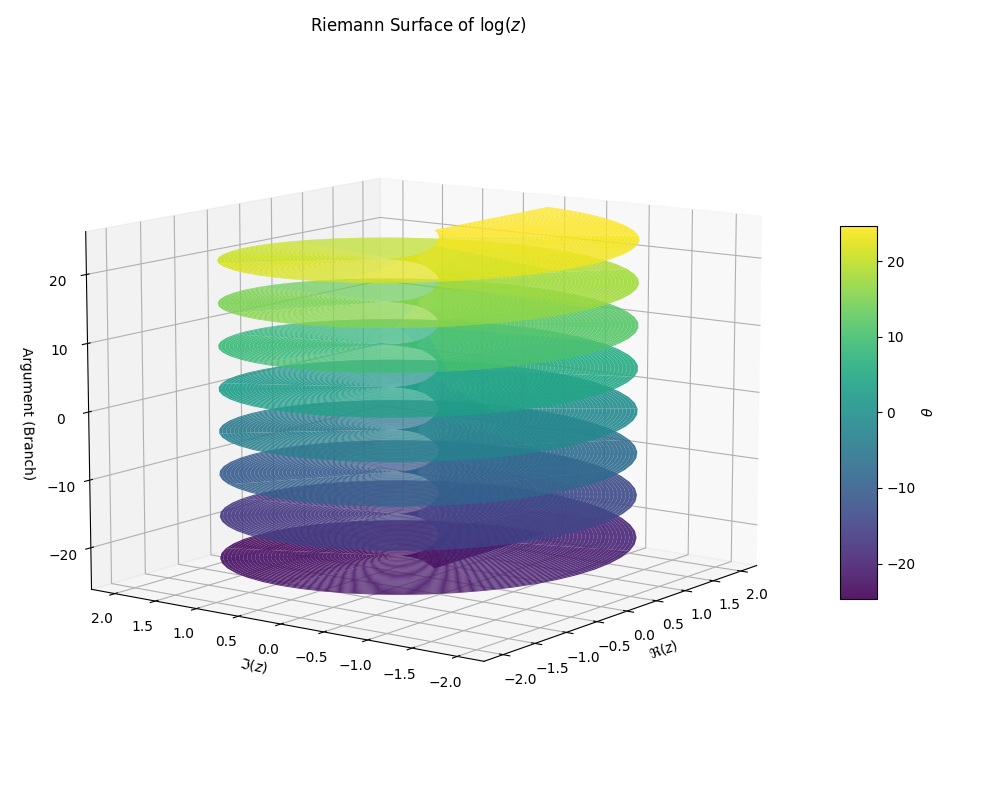
\includegraphics[width=0.85\textwidth]{chapters/chp7_pics/riemann_log.png}
\caption{\textit{The Riemann surface of $\Log(z)$, a helical structure where each sheet represents a branch of $\ln(z)$ for $k \in \mathbb{Z}$, connected along the branch cut at the negative real axis. As $z$ circles the origin, the imaginary part ascends or descends through layers, with $\Log(z)$ as the principal sheet ($-\pi < \Arg(z) \leq \pi$).}}
\label{fig:log-riemann-surface}
\end{figure}

\exampleline
\begin{example}
Compute all values of $\ln(i)$ and the principal value on the Riemann surface.

\begin{solution}
Write $i = e^{i\pi/2}$:
\[
\ln(i) = \ln 1 + i \left( \frac{\pi}{2} + 2\pi k \right) = i \frac{\pi}{2} (1 + 4k), \quad k \in \mathbb{Z},
\]
giving values like $i\pi/2$, $i 5\pi/2$, $i (-\pi/2)$, each on a distinct sheet of the Riemann surface. The principal branch ($-\pi < \Arg(z) \leq \pi$) selects:
\[
\Log(i) = i \frac{\pi}{2},
\]
since $\pi/2$ fits within $(-\pi, \pi]$, anchoring this value to the base sheet.
\end{solution}
\end{example}
\exampleline

\noindent The logarithm’s layered nature, beautifully captured by its Riemann surface, primes us for the next subsection on branch cuts, where we’ll slice through this helical expanse to navigate its many dimensions.

\subsection*{Multiple-Valued Functions and Branch Cuts} \index{Branch Cuts}

\noindent The complex logarithm’s multi-valued nature, stacking outputs like $\ln(-1) = i\pi (1 + 2k)$, hints at a broader phenomenon in $\mathbb{C}$: many functions assign multiple values to a single input. Take the square root: for $z = 4$, $w = 2$ and $w = -2$ both satisfy $w^2 = 4$, doubling the real case. For $z = r e^{i\theta}$, $z^{1/2} = \sqrt{r} e^{i\theta/2}$ or $\sqrt{r} e^{i(\theta/2 + \pi)}$, a pair tied to $e^{i\pi} = -1$. Similarly, $z^{1/n}$ yields $n$ roots, $r^{1/n} e^{i(\theta + 2\pi k)/n}$, $k = 0, 1, \ldots, n-1$, cycling around the origin. \\

\noindent To pin these down, we use \textbf{branch cuts}—lines where we restrict the function to a single \textbf{branch}. For $\ln(z)$, the negative real axis cut gives $\Log(z) = \ln|z| + i \Arg(z)$, $\Arg(z) \in (-\pi, \pi]$. Power functions like $z^{1/3}$ often adopt the same cut, selecting one of three roots. Inverse trigonometric functions, say $\arcsin(z)$, cut from $-\infty$ to $-1$ and $1$ to $\infty$, picking a principal path from infinite possibilities. These cuts, arbitrary yet purposeful, echo the Riemann surface’s layers, slicing a single sheet from the spiral stack. \\

\exampleline
\begin{example}
Find the principal value of $(-8)^{1/3}$, cut along the negative real axis, $\Arg(z) \in (-\pi, \pi]$.

\begin{solution}
Write $-8 = 8 e^{i\pi}$: $(-8)^{1/3} = 8^{1/3} e^{i(\pi + 2\pi k)/3} = 2 e^{i(\pi/3 + 2\pi k/3)}$. For $k = 0, 1, 2$:
\begin{itemize}
\item $k = 0$: $2 e^{i\pi/3} = 1 + i\sqrt{3}$ ($\Arg = \pi/3$),
\item $k = 1$: $2 e^{i\pi} = -2$ ($\Arg = \pi$),
\item $k = 2$: $2 e^{i 5\pi/3} = 1 - i\sqrt{3}$ ($\Arg = -\pi/3$).
All fit $(-\pi, \pi]$, but $k = 0$ is typically principal: $1 + i\sqrt{3}$.
\end{itemize}
\end{solution}
\end{example}
\exampleline

\noindent Branch cuts thus refine multi-valued functions into single-valued tools, their placement shaping our journey through $\mathbb{C}$’s layered expanse.

\subsection*{Computer-Aided Visualization} \index{Complex Visualization Software}

\noindent As we’ve journeyed through the complex plane, from polynomials to logarithms, static sketches have hinted at the richness of these functions. Yet, in an era of digital prowess, software unfurls a new dimension of exploration, breathing life into complex mappings with tools that twist, spin, and zoom at our command. These programs don’t merely draw—they invite us to interact with the mathematics, revealing dynamics that paper alone can’t capture. A direct plot of a complex function, mapping one two-dimensional plane to another, demands four dimensions—a feat beyond a simple page—but computational tools rise to the challenge with elegant solutions like domain coloring. \\

\noindent Domain coloring paints the complex plane with hues and shades to unveil a function’s hidden dance, assigning colors to the range based on its properties. We let \textbf{hue} reflect the argument of $f(z)$, the angle it makes in the plane—picture a color wheel where red marks 0, yellow $\pi/2$, green $\pi$, cycling through the spectrum over $2\pi$—while \textbf{brightness} mirrors the magnitude $|f(z)|$, bright where it soars, dark where it dips. What emerges is a vivid tapestry: \textbf{zeros} appear as dark points, colors converging since $|f(z)|$ vanishes; \textbf{poles} blaze bright, hues spiraling tightly; \textbf{branch cuts} slice as sharp discontinuities—think of $\ln(z)$’s jump from $\pi$ to $-\pi$—and \textbf{periodicity} unfurls in repeating bands. Consider $f(z) = z^2$: software reveals its zero at the origin as a dark center, with hues doubling around it, a visual echo of $\arg(z^2) = 2\arg(z)$. \\

\begin{figure}[H]
\centering
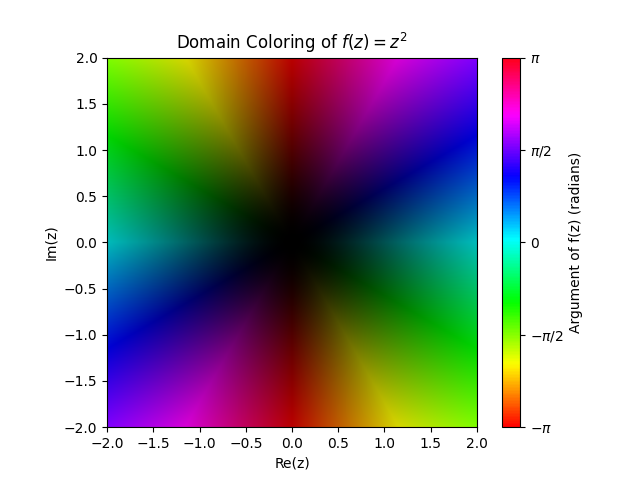
\includegraphics[width=0.8\textwidth]{chapters/chp7_pics/domain_coloring.png}
\caption{\textit{Domain coloring of $f(z) = z^2$, where hue encodes the argument of $f(z)$, ranging from $-\pi$ to $\pi$ to span all directions in the complex plane once, and brightness reflects the magnitude $|f(z)|$ on a logarithmic scale. The doubled cycling of hues around the dark center reveals the angle-doubling property, $\arg(z^2) = 2\arg(z)$, a hallmark of this quadratic mapping.}}
\label{fig:domain-coloring-z2}
\end{figure}

%\noindent You can use this code to provide a domain coloring in Python. \\


\vspace{1.3em} \index{Python}


\begin{lstlisting}[language=Python]
import numpy as np
import matplotlib.pyplot as plt
from matplotlib.colors import hsv_to_rgb
from matplotlib.cm import ScalarMappable

# Define the complex function f(z) = z^2
f = lambda z: z**2

# Set up the grid in the complex plane
x = np.linspace(-2, 2, 400)
y = np.linspace(-2, 2, 400)
X, Y = np.meshgrid(x, y)
Z = X + 1j * Y

# Compute f(z)
W = f(Z)

# Calculate magnitude and argument
magnitude = np.abs(W)
argument = np.angle(W)

# Normalize magnitude for brightness (log scale for better contrast)
magnitude = np.log1p(magnitude)
magnitude = (magnitude - np.min(magnitude)) / (np.max(magnitude) - np.min(magnitude))

# Create HSV image: hue from argument, full saturation, value from magnitude
h = (argument + np.pi) / (2 * np.pi)  # Hue: 0 to 1
s = np.ones_like(h)                   # Saturation: full
v = magnitude                         # Value: brightness
hsv = np.dstack((h, s, v))

# Convert HSV to RGB for plotting
rgb = hsv_to_rgb(hsv)

# Generate the plot
plt.imshow(rgb, extent=(-2, 2, -2, 2), origin='lower')
plt.title(r'Domain Coloring of $f(z) = z^2$')
plt.xlabel('Re(z)')
plt.ylabel('Im(z)')

# Add colorbar for argument
sm = ScalarMappable(cmap='hsv', norm=plt.Normalize(-np.pi, np.pi))
sm.set_array([])  # Required for colorbar to work with ScalarMappable
cbar = plt.colorbar(sm, label='Argument of f(z) (radians)')
cbar.set_ticks([-np.pi, -np.pi/2, 0, np.pi/2, np.pi])
cbar.set_ticklabels([r'$-\pi$', r'$-\pi/2$', r'$0$', r'$\pi/2$', r'$\pi$'])

plt.show()

\end{lstlisting}
\vspace{1.1cm}

\noindent Beyond domain coloring, software offers more wonders: \textbf{interactive plots} let you click a domain point and see its range image, or drag to trace preimages; \textbf{real-time parameter tweaks} shift $f(z) = z^2 + c$ instantly; \textbf{animations} layer transformations like $e^z$ atop $z^2$; and \textbf{surface plots of $|f(z)|$} offer a topographic view of magnitude. These tools sharpen our grasp of \textbf{geometric effects}—addition nudges, multiplication rotates, as with $i z$ at 90 degrees—while zooming near \textbf{singular points} reveals poles flaring or essential singularities writhing. For \textbf{multi-valued functions}, software peels apart branches, stacking $\ln(z)$’s layers, and previews \textbf{conformal mappings}’ angle preservation, as grids bend yet hold shape. \\

\noindent Take $f(z) = e^z$: software maps a grid—horizontal lines to rays, verticals to circles—letting you tilt the view or animate $z$’s path, the output spiraling in rhythm. This builds on the static depiction in Figure \ref{fig:exp-mapping}, amplifying what such figures suggest and opening a window into the function’s soul. \\

\noindent Software also lifts us into three dimensions, offering vivid perspectives on complex functions beyond the flat plane. One approach plots the \textbf{magnitude $|f(z)|$} as a surface over the domain, with height revealing growth—zeros dip to the plane, poles spike skyward, and the function’s scale unfurls in a topographic sweep. For $f(z) = z^2$, this surface rises parabolically from its zero at the origin, a 3D testament to its quadratic stretch across the plane.

\begin{figure}[h]
\centering
\begin{tikzpicture}
\begin{axis}[
    width=0.8\textwidth,
    height=0.6\textwidth,
    axis lines=center,
    title={Magnitude of $f(z) = z^2$},
    view={120}{30},
    colormap/viridis,
    colorbar,
    colorbar style={ylabel=$|f(z)|$},
    xtick=\empty,
    ytick=\empty,
    ztick=\empty,
]
\addplot3 [
    surf,
    domain=-2:2,
    y domain=-2:2,
    samples=30,
] {x^2 + y^2};

% Add movable labels
\node at (axis cs:1.7,0.1,0) [anchor=west] {$\Re(z)$};
\node at (axis cs:0,2,0) [anchor=south] {$\Im(z)$};
\node at (axis cs:0,0.2,8) [anchor=south] {$|f(z)|$};
\end{axis}
\end{tikzpicture}
\caption{Surface plot of $|f(z)| = |z^2|$ over the complex plane, with height showing magnitude rising quadratically from the zero at the origin.}
\label{fig:magnitude-z2}
\end{figure}

\noindent Alternatively, software can surface the \textbf{real or imaginary parts}, plotting $u(x, y)$ or $v(x, y)$ to trace their undulations over the complex plane. Take $f(z) = e^z$: its real part $e^x \cos y$ blends exponential growth along the real axis with cosine waves along the imaginary, a 3D ripple that echoes its oscillatory nature. Then there’s the \textbf{Riemann surface}, stacking multi-valued outputs like $\ln(z)$’s spiral sheets, as seen in Figure \ref{fig:log-riemann-surface}, where branches connect across cuts in a helical dance. These 3D views—crafted by tools like Python or Mathematica—bring the invisible into focus, marrying computation with intuition.

\begin{figure}[h]
\centering
\begin{tikzpicture}
\begin{axis}[
    width=0.8\textwidth,
    height=0.6\textwidth,
    axis lines=center,
    title={Real Part of $f(z) = e^z$},
    view={120}{30},
    colormap/viridis,
    colorbar,
    colorbar style={ylabel=$\Re(f(z))$},
    xtick=\empty,  % Remove x-axis ticks
    ytick=\empty,  % Remove y-axis ticks
    ztick=\empty,  % Remove z-axis ticks
]
\addplot3 [
    surf,
    domain=-2:2,
    y domain=-3.1416:3.1416,
    samples=30,
] {exp(x)*cos(deg(y))};

% Movable labels
\node at (axis cs:2,0.2,0) [anchor=west] {$\Re(z)$};         % Label for Re(z)
\node at (axis cs:0,3.1416,0) [anchor=south] {$\Im(z)$};   % Label for Im(z)
\node at (axis cs:0,0,7.4) [anchor=south] {$\Re(f(z))$};   % Label for Re(f(z))
\end{axis}
\end{tikzpicture}
\caption{Surface plot of the real part of $f(z) = e^z$, where $u(x, y) = e^x \cos y$ blends exponential growth along the real axis with cosine oscillations along the imaginary.}
\label{fig:real-exp}
\end{figure}

\noindent These visualizations, from domain coloring to 3D surfaces, are ingenious compromises. A complex function \( f: \mathbb{C} \to \mathbb{C} \) demands four dimensions—two for the input \( z \), two for the output \( f(z) \)—but our tools are bound to three or two. Domain coloring squeezes both magnitude and argument into a 2D image via color, while surface plots of \( |f(z)| \), \( \Re(f(z)) \), or \( \Im(f(z)) \) reduce the output to one real number, plotted over the complex plane in 3D. Riemann surfaces stack multi-valued outputs, hinting at the function's layers. Each method sacrifices a dimension to make the invisible visible, offering a glimpse into the function's soul at the cost of completeness.

\newpage
\lecture{Basic Limits in Complex Analysis} \index{Limits}

\noindent In Chapter 3, Lecture 2, we developed the epsilon–delta definition of limits for functions in \(\mathbb{R}^n\). When we move into complex analysis, the formal definition remains identical—using the modulus \(|z-z_0|\) as our measure of distance—but the two-dimensional nature of \(\mathbb{C}\) and its algebraic structure open up additional techniques for evaluating limits. In this lecture, we expand on the basics of complex limits, highlight methods unique to the complex setting, and explain in detail how to handle expressions involving complex conjugates.

\subsection*{Basic Definition and Similarities}

\noindent Let \(f: D \to \mathbb{C}\) be a function defined on a domain \(D \subseteq \mathbb{C}\), and let \(z_0\) be a limit point of \(D\). We say that 
\[
\lim_{z \to z_0} f(z) = L
\]
if for every \(\epsilon > 0\) there exists a \(\delta > 0\) such that for all \(z \in D\) with \(0 < |z - z_0| < \delta\) we have
\[
|f(z) - L| < \epsilon.
\]
This is exactly the epsilon–delta definition used in \(\mathbb{R}^n\), with the key difference that here distance is measured by the modulus \(|z-z_0|\). Because \(\mathbb{C}\) is essentially \(\mathbb{R}^2\), many aspects of higher-dimensional limits carry over directly. However, the two-dimensional nature of \(\mathbb{C}\) introduces an important nuance: there are infinitely many directions from which \(z\) can approach \(z_0\). \\

\noindent In \(\mathbb{R}^n\), we typically consider sequences or paths converging to a point and verify that the limit is independent of the chosen path. In \(\mathbb{C}\), this requirement is even more critical. For the limit \(L\) to exist, the condition \(|f(z) - L| < \epsilon\) must hold regardless of the angle or path along which \(z\) approaches \(z_0\). This path-independence guarantees the uniqueness of the limit and is automatically satisfied in one-dimensional real analysis, but must be explicitly checked in the complex setting. Thus, while the definition is formally the same as in \(\mathbb{R}^n\), the complex case forces us to account for a richer set of approaches to a limit point.



\begin{figure}[H]
\centering
\begin{tikzpicture}[scale=1.5]
  % Draw axes
  \draw[->] (-1.5,0) -- (1.5,0) node[right] {$\Re(z)$};
  \draw[->] (0,-1.5) -- (0,1.5) node[above] {$\Im(z)$};

  % Draw open disk (dotted border)
  \fill[blue, opacity=0.2] (0.5,0.5) circle (0.8);
  \draw[blue, thick, dotted] (0.5,0.5) circle (0.8);

  % Mark z_0
  \fill (0.5,0.5) circle (1pt);
  \node at (0.55,0.65) {$z_0$};  % Move this coordinate to adjust label position

  % Radius arrow
  \draw[->] (0.5,0.5) -- (1.3,0.5) node[midway, above] {$\epsilon$};
\end{tikzpicture}
\caption{An open disk \(D(z_0, \epsilon)\) centered at \(z_0\) with radius \(\epsilon\) in the complex plane.}
\label{fig:open-disk}
\end{figure}


\subsection*{New Techniques in Evaluating Complex Limits}

\noindent Although the basic epsilon–delta definition remains unchanged, several additional techniques are especially useful in complex analysis:

\begin{itemize}
    \item \textbf{Use of Polar Form:} Expressing a complex number \(z\) in polar coordinates as
    \[
    z = re^{i\theta},
    \]
    where \(r = |z|\) and \(\theta = \arg(z)\), can simplify the evaluation of limits. In many cases, limits reduce to a function of \(r\) (the distance from the origin) and \(\theta\) (the angle of approach). This method also helps us check if the limit is path-independent; if the limit depends on \(\theta\), it does not exist.
    
    \item \textbf{Series Expansion:} Similar to real analysis, Taylor series expansions for functions such as \(\sin(z)\), \(\cos(z)\), or \(e^z\) allow us to approximate and evaluate limits. For example, expanding \(\sin(z)\) as
    \[
    \sin(z) = z - \frac{z^3}{3!} + \frac{z^5}{5!} - \cdots,
    \]
    simplifies the evaluation of \(\frac{\sin(z)}{z}\) as \(z\) approaches 0.
    
    \item \textbf{Handling Complex Conjugates:} Complex conjugates play a special role in \(\mathbb{C}\). If \(z = re^{i\theta}\), then the conjugate is given by
    \[
    \overline{z} = re^{-i\theta}.
    \]
    This relationship is extremely useful in simplifying expressions where both \(z\) and \(\overline{z}\) appear. For example, note that \(|z|^2 = z\overline{z}\) and that ratios like \(\frac{\overline{z}}{z}\) can be expressed in terms of the argument \(\theta\), as we will see.
    
    \item \textbf{Modulus and Argument Techniques:} By decomposing a complex number into its modulus and argument, we can often determine if a limit is well-defined. If the limit expression depends on the angle \(\theta\) (i.e., the direction of approach), then the limit might not exist. This method is particularly useful when dealing with functions that do not behave uniformly in every direction.
\end{itemize}

\noindent A common scenario in complex limits is the appearance of the complex conjugate. Consider the ratio:
\[
\frac{\overline{z}}{z}.
\]
Express \(z\) in polar form as \(z = re^{i\theta}\). Then the conjugate is \(\overline{z} = re^{-i\theta}\), and the ratio simplifies to
\[
\frac{\overline{z}}{z} = \frac{re^{-i\theta}}{re^{i\theta}} = e^{-2i\theta}.
\]
Here, the modulus of the expression is always 1, but its value depends entirely on the angle \(\theta\). As \(z \to 0\), although \(r\) tends to 0, the value of \(\theta\) may vary depending on the path taken toward the origin. For example:
\begin{itemize}
    \item Along the positive real axis (\(\theta = 0\)), \(e^{-2i\theta} = 1\).
    \item Along the positive imaginary axis (\(\theta = \pi/2\)), \(e^{-2i\theta} = e^{-i\pi} = -1\).
\end{itemize}
Since the limit depends on the direction of approach, the limit of \(\frac{\overline{z}}{z}\) as \(z \to 0\) does not exist.

\subsection*{Properties of Limits in \(\mathbb{C}\)}

\noindent The algebraic properties of limits that you are familiar with from real analysis extend naturally to complex functions. Suppose that 
\[
\lim_{z \to z_0} f(z) = L \quad \text{and} \quad \lim_{z \to z_0} g(z) = M.
\]
Then the following properties hold:
\begin{itemize}
  \item \(\displaystyle \lim_{z \to z_0} \bigl(f(z) + g(z)\bigr) = L + M\).
  \item \(\displaystyle \lim_{z \to z_0} \bigl(f(z) \cdot g(z)\bigr) = L \cdot M\).
  \item For any constant \(c \in \mathbb{C}\), \(\displaystyle \lim_{z \to z_0} c\,f(z) = c\,L\).
  \item If \(M \neq 0\), \(\displaystyle \lim_{z \to z_0} \frac{f(z)}{g(z)} = \frac{L}{M}\).
\end{itemize}
These properties rely on the fact that the modulus \(|\cdot|\) in \(\mathbb{C}\) obeys the triangle inequality and product rule, much like the Euclidean norm in \(\mathbb{R}^2\). The proofs of these properties follow along the same lines as in Chapter 3, Lecture 2, and serve as a useful bridge between real and complex analysis.

\exampleline
\begin{example}
Evaluate the following limits:
\begin{enumerate}
    \item \( \displaystyle \lim_{z \to 0} z^2 \)
    \item \( \displaystyle \lim_{z \to 0} \frac{\sin(z)}{z} \)
    \item \( \displaystyle \lim_{z \to 0} \frac{|z|^2}{z} \)
    \item \( \displaystyle \lim_{z \to 0} \frac{\overline{z}}{z} \)
\end{enumerate}

\begin{solution}
\begin{enumerate}
    \item \textbf{Limit of \(z^2\):}  
    Since \(z^2\) is a polynomial, it is continuous everywhere in \(\mathbb{C}\). Therefore, by direct substitution:
    \[
    \lim_{z \to 0} z^2 = 0^2 = 0.
    \]

    \item \textbf{Limit of \(\frac{\sin(z)}{z}\):}  
    The Taylor series for \(\sin(z)\) is:
    \[
    \sin(z) = z - \frac{z^3}{3!} + \frac{z^5}{5!} - \cdots.
    \]
    Dividing by \(z\) yields:
    \[
    \frac{\sin(z)}{z} = 1 - \frac{z^2}{3!} + \frac{z^4}{5!} - \cdots.
    \]
    As \(z \to 0\), all terms involving \(z\) vanish, hence:
    \[
    \lim_{z \to 0} \frac{\sin(z)}{z} = 1.
    \]

    \item \textbf{Limit of \(\frac{|z|^2}{z}\):}  
    Recall that \(|z|^2 = z \overline{z}\). Thus, for \(z \neq 0\):
    \[
    \frac{|z|^2}{z} = \frac{z\overline{z}}{z} = \overline{z}.
    \]
    As \(z \to 0\), \(\overline{z} \to 0\) (since complex conjugation is continuous), so:
    \[
    \lim_{z \to 0} \frac{|z|^2}{z} = 0.
    \]

    \item \textbf{Limit of \(\frac{\overline{z}}{z}\):}  
    Write \(z = re^{i\theta}\) so that \(\overline{z} = re^{-i\theta}\). Then,
    \[
    \frac{\overline{z}}{z} = e^{-2i\theta}.
    \]
    Since this expression depends on the angle \(\theta\) and not on the magnitude \(r\), different paths to 0 (with different \(\theta\)) yield different values. For example:
    \begin{itemize}
        \item If \(z\) approaches 0 along the positive real axis (\(\theta=0\)), then \(\frac{\overline{z}}{z} = 1\).
        \item If \(z\) approaches 0 along the positive imaginary axis (\(\theta=\pi/2\)), then \(\frac{\overline{z}}{z} = e^{-i\pi} = -1\).
    \end{itemize}
    Therefore, the limit does not exist.
\end{enumerate}
\end{solution}
\end{example}
\exampleline

\noindent In summary, while the fundamental definition of limits in \(\mathbb{C}\) mirrors that in \(\mathbb{R}^n\), the additional structure of complex numbers allows us to employ techniques such as polar representation and series expansions. These methods, along with careful treatment of expressions involving complex conjugates, are essential tools in evaluating complex limits and in detecting path-dependent behavior.


\subsection*{Continuity and Topological Foundations in \(\mathbb{C}\)}

\noindent In complex analysis, the notion of continuity is defined in exactly the same way as in real analysis using the epsilon–delta formulation. However, the two-dimensional structure of \(\mathbb{C}\) and its rich topology provide additional tools and perspectives that are crucial for a deeper understanding of limits and continuity. In this section, we discuss these foundational ideas and illustrate their usefulness with detailed examples.

\subsubsection*{Continuity in \(\mathbb{C}\)}

\noindent Let \(f: D \to \mathbb{C}\) be a function on a domain \(D \subseteq \mathbb{C}\) and let \(z_0\) be a limit point of \(D\). We say that 
\[
\lim_{z \to z_0} f(z) = L
\]
if for every \(\epsilon > 0\) there exists a \(\delta > 0\) such that whenever \(z \in D\) with \(0 < |z-z_0| < \delta\) it follows that
\[
|f(z) - L| < \epsilon.
\]
This definition uses the modulus \(|z-z_0|\) as the distance measure, leveraging the fact that \(\mathbb{C}\) is isometric to \(\mathbb{R}^2\).

An equivalent formulation employs open sets: \(f\) is continuous at \(z_0\) if for every open neighborhood \(V\) of \(f(z_0)\) there is an open neighborhood \(U\) of \(z_0\) such that
\[
f(U) \subseteq V.
\]
In \(\mathbb{C}\), open neighborhoods are typically open disks of the form
\[
D(z_0, \epsilon) = \{ z \in \mathbb{C} : |z-z_0| < \epsilon \}.
\]
\exampleline
\begin{example}
Consider the function \(f(z) = |z|^2 = z\overline{z}\). Show that \(f\) is continuous at any \(z_0 \in \mathbb{C}\).
\begin{solution}
Let \(\epsilon > 0\) be given. We wish to find a \(\delta > 0\) such that for all \(z\) with \(|z-z_0| < \delta\),
\[
\bigl||z|^2 - |z_0|^2\bigr| = |z\overline{z} - z_0\overline{z_0}| < \epsilon.
\]
Notice that
\[
|z\overline{z} - z_0\overline{z_0}| = |z(\overline{z}-\overline{z_0}) + \overline{z_0}(z-z_0)| \leq |z||z-z_0| + |z_0||z-z_0|.
\]
Since \(|z-z_0|<1\) implies \(|z| \le |z_0| + 1\), we have
\[
|f(z) - f(z_0)| < \bigl((|z_0|+1) + |z_0|\bigr)|z-z_0| = (1+2|z_0|)|z-z_0|.
\]
Thus, choosing
\[
\delta = \min\left\{1,\,\frac{\epsilon}{1+2|z_0|}\right\},
\]
ensures that \(|f(z)-f(z_0)| < \epsilon\) whenever \(|z-z_0| < \delta\). Hence, \(f\) is continuous at \(z_0\).
\end{solution}
\end{example}
\exampleline
\subsubsection*{Topological Properties of \(\mathbb{C}\) and Their Usefulness}

The rich topological structure of \(\mathbb{C}\) – inherited from its homeomorphism with \(\mathbb{R}^2\) – provides us with powerful tools such as open sets, connectedness, and compactness, which are essential for rigorously understanding limits and continuity. In the following sections, we will develop these technical foundations further to deepen our understanding of continuity in complex analysis.\\

\noindent \textbf{Open Sets:} \noindent One of the cornerstones of topology—and by extension, of continuity and limit theory—is the concept of an open set. In Chapter 3, Lecture 2, we covered the basics of open sets in \(\mathbb{R}^n\). Since \(\mathbb{C}\) is very similar to \(\mathbb{R}^2\), these ideas translate directly to the complex plane with an added geometric elegance.\\

\noindent In \(\mathbb{C}\), every open set can be expressed as a union of open disks. An open disk centered at \(z_0\) with radius \(\epsilon\) is defined by
\[
D(z_0, \epsilon) = \{ z \in \mathbb{C} : |z - z_0| < \epsilon \}.
\]
This disk is the basic building block or ``neighborhood" of \(z_0\) in the complex plane. It provides a precise way to describe what it means for points to be ``close" to \(z_0\) using the modulus as a distance measure. \\

\noindent The usefulness of open disks becomes evident when we prove local properties like continuity. Specifically, to show that a function \(f\) is continuous at a point \(z_0\), one must show that for every open disk \(D(f(z_0), \eta)\) around \(f(z_0)\) in the codomain, there exists an open disk \(D(z_0, \epsilon)\) around \(z_0\) in the domain such that
\[
f\bigl(D(z_0, \epsilon)\bigr) \subseteq D(f(z_0), \eta).
\]
This topological formulation is entirely equivalent to the epsilon–delta definition but emphasizes the spatial, geometric intuition behind continuity.

\exampleline
\begin{example}
Consider again \(f(z)=z^2\). Demonstrate that for any open disk \(D(z_0, \epsilon)\) centered at \(z_0\), there exists an open disk \(D(f(z_0), \eta)\) such that
\[
f\bigl(D(z_0, \epsilon)\bigr) \subseteq D(f(z_0), \eta).
\]
\begin{solution}
Since \(f(z)=z^2\) is continuous, for any \(\eta > 0\) there exists \(\delta > 0\) so that if \(|z-z_0| < \delta\) then
\[
|z^2-z_0^2| = |z-z_0||z+z_0| < \eta.
\]
By choosing \(\delta\) sufficiently small (ensuring, for example, that \(|z-z_0| < 1\) so that \(|z+z_0|\) is bounded), we guarantee that the entire disk \(D(z_0, \delta)\) is mapped inside \(D(z_0^2, \eta)\). 
\end{solution}
\end{example}
\exampleline

\noindent \textbf{Connectedness:}  The complex plane \(\mathbb{C}\) is a prime example of a connected space—it is not only connected but also path-connected. This means that for any two points \(z_1, z_2 \in \mathbb{C}\), there exists a continuous path \(\gamma: [0,1] \to \mathbb{C}\) such that \(\gamma(0)=z_1\) and \(\gamma(1)=z_2\). In practical terms, this property implies that the complex plane cannot be split into two disjoint nonempty open subsets.  \\

\noindent Connectedness has profound implications in analysis. One of the key theorems states that if a function \(f: D \to \mathbb{C}\) is continuous on a connected domain \(D\), then the image \(f(D)\) is also connected. This result is critical because it ensures that continuous functions cannot “break apart” the domain into separate pieces. As a consequence, if a continuous function takes two distinct values on a connected set, it must take every value in between (this is an extension of the intermediate value property to connected sets in \(\mathbb{C}\)). \\

\noindent The equivalence of connectedness and path-connectedness in \(\mathbb{C}\) (a feature of all metric spaces like \(\mathbb{R}^2\)) further simplifies many arguments. When dealing with limits and continuity, knowing that any two points are joined by some continuous path allows us to analyze function behavior along various paths and conclude that the limit (or image) must be the same regardless of the chosen path.


\begin{example}
Let \(f(z) = e^z\). Prove that \(e^{\mathbb{C}}\) is connected.
\begin{solution}
The function \(f(z)=e^z\) is continuous and maps \(\mathbb{C}\) onto \(\mathbb{C}\setminus\{0\}\). Since \(\mathbb{C}\) is path-connected, any continuous image of \(\mathbb{C}\) must be connected. Therefore, \(e^{\mathbb{C}} = \mathbb{C}\setminus\{0\}\) is connected.
\end{solution}
\end{example}

\begin{figure}[H]
\centering
\begin{tikzpicture}[scale=1.5]
  \draw[->, thick] (-0.5,0) -- (2,0) node[right] {$\Re(z)$};
  \draw[->, thick] (0,-0.5) -- (0,2) node[above] {$\Im(z)$};
  \fill (0.5,0.5) circle (2pt) node[below left] {\(z_1\)};
  \fill (1.5,1.2) circle (2pt) node[above right] {\(z_2\)};
  \draw[red, thick, ->] (0.5,0.5) .. controls (1,1.5) and (1.2,0.2) .. (1.5,1.2);
\end{tikzpicture}
\caption{Any two points in \(\mathbb{C}\) can be connected by a continuous path.}
\label{fig:connected-path}
\end{figure}

\noindent \textbf{Compactness:}  In the setting of \(\mathbb{C}\) (which, as we know, is essentially \(\mathbb{R}^2\)), a set is called compact if it is both closed and bounded. Here, a set is \emph{closed} if it contains all its boundary points, and it is \emph{bounded} if it can be entirely contained within a disk of some finite radius. This result is known as the \textbf{Heine–Borel theorem}. \index{Heine-Borel Theorem}Compact sets are very useful in analysis because any continuous function defined on a compact set is guaranteed to reach both a maximum and a minimum value—a fact learned earlier as the Extreme Value Theorem. This property helps ensure that functions behave in a controlled manner, which is critical when dealing with limits.
\exampleline
\begin{example}
Let 
\[
A = \{ z \in \mathbb{C} : 1 \leq |z| \leq 2 \}
\]
be the closed annulus in \(\mathbb{C}\). First, show that \(A\) is compact. Then, consider the function 
\[
f(z) = z^2.
\]
Show that \(f\) is continuous on \(A\) and deduce that \(f(A)\) is compact. Finally, determine the range of \(|f(z)|\) on \(A\) and verify that \(f\) attains its maximum and minimum values.

\begin{solution}
\begin{enumerate}
\item \textbf{Prove \(A\) is Compact.}
The set \(A\) is defined by the condition \(1 \leq |z| \leq 2\). It is bounded because every \(z \in A\) satisfies \(|z| \leq 2\), and it is closed because it includes all points on its boundary (those with \(|z|=1\) and \(|z|=2\)). By the Heine–Borel theorem, every closed and bounded subset of \(\mathbb{R}^2\) is compact. Since \(\mathbb{C}\) is homeomorphic to \(\mathbb{R}^2\), \(A\) is compact.

\item \textbf{Show \(f(z) = z^2\) is Continuous on \(A\) and \(f(A)\) is Compact.}
Since \(f(z)=z^2\) is a polynomial, it is continuous on the entire complex plane, and in particular on the compact set \(A\). The continuous image of a compact set is compact, so \(f(A)\) is compact.

\item \textbf{Determine the Range of \(|f(z)|\) on \(A\).}
Notice that for any \(z \in \mathbb{C}\),
\[
|f(z)| = |z^2| = |z|^2.
\]
Since \(z \in A\) satisfies \(1 \leq |z| \leq 2\), we have:
\[
1^2 \leq |z|^2 \leq 2^2 \quad \Longrightarrow \quad 1 \leq |f(z)| \leq 4.
\]
Thus, the minimum modulus of \(f(z)\) on \(A\) is 1, and the maximum modulus is 4. These extreme values are attained when \(|z| = 1\) (yielding \(|f(z)| = 1\)) and when \(|z| = 2\) (yielding \(|f(z)| = 4\)), respectively.

\item \textbf{Conclusion:}
We have shown that the closed annulus 
\[
A = \{ z \in \mathbb{C} : 1 \leq |z| \leq 2 \}
\]
is compact. The function \(f(z) = z^2\) is continuous on \(A\), so its image \(f(A)\) is also compact. Moreover, since \(|f(z)| = |z|^2\), the range of \(|f(z)|\) on \(A\) is the interval \([1,4]\), meaning that \(f\) attains a minimum modulus of 1 and a maximum modulus of 4 on \(A\).

\end{enumerate}
\end{solution}
\end{example}
\exampleline

\noindent \textbf{Extended Complex Plane:} To study limits that involve behavior ``at infinity,” it is useful to introduce the extended complex plane, denoted
\[
\hat{\mathbb{C}} = \mathbb{C} \cup \{\infty\}.
\]
This construction ``adds” a single point at infinity to \(\mathbb{C}\), thereby compactifying the plane and making it homeomorphic to the Riemann sphere. In other words, by including \(\infty\), we transform \(\mathbb{C}\) from an unbounded space into a compact space, which has many desirable properties in analysis. \\

\noindent One major advantage of working in the extended complex plane is that it allows us to handle limits at infinity in a manner analogous to limits at finite points. Specifically, we define
\[
\lim_{z \to \infty} f(z) = L
\]
if, for every \(\epsilon > 0\), there exists an \(R > 0\) such that whenever \(|z| > R\) (that is, \(z\) lies outside a disk of radius \(R\)), it follows that
\[
|f(z) - L| < \epsilon.
\]
\noindent This definition mirrors the standard epsilon–delta definition of a limit, but with the roles reversed: instead of \(z\) approaching a specific finite point, we require the values of \(f(z)\) to approach \(L\) as \(z\) ``escapes” to infinity. \\

\noindent The compactification of \(\mathbb{C}\) via the addition of \(\infty\) is not merely a technical trick—it has significant consequences. For example, many theorems that hold on compact sets (such as the Extreme Value Theorem) can now be extended to functions defined on \(\hat{\mathbb{C}}\). Moreover, considering limits at infinity in this framework unifies our approach to finite and infinite limits. \\

\noindent To visualize the extended complex plane, one often uses the Riemann sphere. Imagine the complex plane as the equatorial plane of a sphere. Each point in \(\mathbb{C}\) corresponds to a point on the sphere via stereographic projection, and the ``north pole” of the sphere represents the point at infinity. This geometric picture helps us understand how sequences that ``escape” to infinity in \(\mathbb{C}\) are seen as converging to the north pole on the Riemann sphere.

\begin{figure}[H]
\centering
\begin{tikzpicture}[scale=1.2]

  % Draw the outer circle representing the sphere
  \draw[thick] (0,0) circle (2cm);
  
  % Draw the "equator" as a horizontal ellipse
  % Dashed back half from left to right
  \draw[dashed, thick] (-2,0) arc (180:360:2cm and 0.7cm);
  % Solid front half from right to left
  \draw[thick] (2,0) arc (0:180:2cm and 0.7cm);
  
  % Mark the north pole (representing infinity)
  \fill (0,2) circle (2pt) node[above] {North Pole (\(\infty\))};
  
  % Mark the south pole
  \fill (0,-2) circle (2pt) node[below] {South Pole};
  
  % Approximate positions of 1, -1, i, and -i on the equator
  % We'll place them around the circle at cardinal points for illustration.
  
  % Right intersection (approx) for z=1
  \fill (2,0) circle (2pt) node[right] {$1$};
  
  % Left intersection (approx) for z=-1
  \fill (-2,0) circle (2pt) node[left] {$-1$};
  
  % Intersection near the "front" of the equator for z=i (we'll place it above the center)
  % Since this is a 2D projection, let's approximate i at some arc in the top half of the equator
  % We can place it at a param or angle. Let's do something simpler:
  \fill (0,0.7) circle (2pt) node[above=2pt] {$i$};
  
  % Intersection near the "front" of the equator for z=-i (we'll place it below the center)
  \fill (0,-0.7) circle (2pt) node[below=2pt] {$-i$};
  
  % We might optionally label the equator or do more arcs if desired
  
\end{tikzpicture}
\caption{A schematic of the Riemann sphere representing the extended complex plane 
\(\hat{\mathbb{C}} = \mathbb{C} \cup \{\infty\}\). The north pole corresponds to the 
point at infinity, while the equator (solid and dashed) is a cross-sectional view of 
the complex plane. The points \(1\), \(-1\), \(i\), and \(-i\) are placed at approximate 
locations on the equator for illustrative purposes.}
\label{fig:riemann-sphere-labeled}
\end{figure}



\exampleline
\begin{example}
Show that
\[
\lim_{z \to 0} \frac{1}{z} = \infty
\]
in the extended complex plane.
\begin{solution}
For \(z \neq 0\),
\[
\left|\frac{1}{z}\right| = \frac{1}{|z|}.
\]
As \(z \to 0\), \(|z|\) becomes arbitrarily small, and consequently, \(\frac{1}{|z|}\) becomes arbitrarily large. Formally, for any \(M > 0\), if we choose \(\delta = \frac{1}{M}\) then whenever \(0 < |z| < \delta\), we have
\[
\left|\frac{1}{z}\right| > M.
\]
Thus, in \(\hat{\mathbb{C}}\), we write
\[
\lim_{z \to 0} \frac{1}{z} = \infty.
\]
This concept is best visualized via the Riemann sphere, where the point at infinity “completes” the compact space.
\end{solution}
\end{example}
\exampleline

\noindent In summary, the topological properties of \(\mathbb{C}\)—including the structure of open sets, connectedness, and compactness, as well as the notion of the extended complex plane—provide a rigorous framework for understanding limits. These properties are essential not only in establishing basic limit results but also in preparing us for more advanced topics in the theory of generalized change.

\subsubsection*{Sequential Continuity in \(\mathbb{C}\)}

\noindent In addition to the epsilon–delta definition, continuity in the complex plane can also be characterized via sequences. Specifically, a function \(f: D \to \mathbb{C}\) is \textbf{sequentially continuous} at a point \(z_0\) if, for every sequence \(\{z_n\}\) in \(D\) converging to \(z_0\), the sequence \(\{f(z_n)\}\) converges to \(f(z_0)\). This viewpoint can be especially intuitive in \(\mathbb{C}\) because there are infinitely many directions from which a point can approach \(z_0\). By considering \emph{all} sequences that converge to \(z_0\), we ensure that the limit of \(f(z)\) is path-independent. If different sequences converging to \(z_0\) yield different limits for \(\{f(z_n)\}\), then \(f\) cannot be continuous at \(z_0\). This sequential perspective thus confirms that continuity demands uniformity of behavior in every direction in the complex plane.

\exampleline
\begin{example}
Consider the function 
\[
f(z) = \frac{\overline{z}}{z}, \quad z \neq 0.
\]
Express \(z\) in polar form as \(z = re^{i\theta}\), so that \(\overline{z} = re^{-i\theta}\). Then,
\[
f(z) = \frac{re^{-i\theta}}{re^{i\theta}} = e^{-2i\theta}.
\]
Now, observe that if we take different sequences approaching 0 with different fixed angles \(\theta\), the value of \(e^{-2i\theta}\) will vary. For instance:
\begin{itemize}
    \item If \(z\) approaches 0 along the positive real axis (\(\theta = 0\)), then \(f(z) = e^0 = 1\).
    \item If \(z\) approaches 0 along the positive imaginary axis (\(\theta = \pi/2\)), then \(f(z) = e^{-i\pi} = -1\).
\end{itemize}
Because the limit depends on the direction of approach, \(f\) is not sequentially continuous at \(z = 0\).
\begin{solution}
Since different sequences approaching \(0\) yield different limit values, by the sequential criterion, \(f(z) = \frac{\overline{z}}{z}\) does not have a unique limit as \(z \to 0\). Hence, \(f\) is not continuous at 0.
\end{solution}
\end{example}
\exampleline

\noindent In conclusion, the interplay between the topology of \(\mathbb{C}\) and the study of limits is central to complex analysis. By understanding open sets, connectedness, and compactness—and by applying both epsilon–delta and sequential definitions of continuity—we establish a robust framework for analyzing how functions behave in the complex plane. This foundational work is indispensable not only for basic limit proofs but also for the more advanced topics that follow. \\

\noindent In particular, these topological and continuity concepts pave the way for \emph{complex differentiability} (also known as \emph{holomorphy}), where a function has a complex derivative at every point in a domain. Holomorphic functions, in turn, exhibit remarkable properties such as \emph{analyticity}, meaning they can be locally represented by power series and have infinitely many derivatives. These deeper results in complex analysis—such as the Cauchy integral theorems, the Maximum Modulus Principle, and analytic continuation—all rely heavily on the topological underpinnings we have established here.  \\

\noindent Thus, by thoroughly understanding limits and continuity in the context of open sets, connected domains, and compact subsets of \(\mathbb{C}\), we equip ourselves with the essential “toolkit” needed to explore the elegant and far-reaching consequences of holomorphic functions in the broader theory of generalized change. 


\newpage




\newpage

\lecture{Complex Differentiation} \index{Complex Differentiation}

\noindent In calculus and real analysis, the derivative is defined as the limit of the difference quotient—a tool that provides the best linear approximation to a function at a given point. But what does it mean to differentiate a function on the complex plane, where every point has infinitely many directions of approach? The idea is similar: we wish for the limit
\[
f'(z_0)=\lim_{\Delta z \to 0}\frac{f(z_0+\Delta z)-f(z_0)}{\Delta z}
\]
to exist. However, because the complex plane is two-dimensional, this limit must be the same regardless of the path along which \(\Delta z\) (or equivalently, \(z-z_0\)) approaches zero. In other words, \(f'(z_0)\) must be independent of the direction of approach. This extra requirement is what makes complex differentiability a much stronger condition than in the real setting.

\subsection*{Motivation and Definition} \index{Holomorphic Functions}

\noindent Recall that every complex number \(z\) can be expressed as
\[
z = x + iy,
\]
and accordingly a function \(f\) defined on a domain \(D\subset\mathbb{C}\) can be written as
\[
f(z)=u(x,y)+iv(x,y).
\]
We say that \(f\) is \textbf{complex differentiable} (or \textbf{holomorphic}) at a point \(z_0\in D\) if
\[
f'(z_0)=\lim_{\Delta z\to 0}\frac{f(z_0+\Delta z)-f(z_0)}{\Delta z}
\]
exists and is independent of the manner in which \(\Delta z\) approaches 0. This condition ensures that, locally, the function can be well-approximated by the linear map
\[
f(z) \approx f(z_0)+f'(z_0)(z-z_0),
\]
where \(f'(z_0)\) acts as both a scaling factor (its modulus \(|f'(z_0)|\)) and a rotation (its angle \(\arg(f'(z_0))\)). In the one-dimensional real setting the function has only two possible directions (from the left or the right), but in \(\mathbb{C}\) there is a continuum of directions. This stronger requirement forces the real and imaginary parts of \(f\) to satisfy interrelated conditions, later formalized as the Cauchy-Riemann equations. \\

\noindent To illustrate the concept, consider the following simplified diagram. The left side shows an \(\epsilon\)-neighborhood (a circle) in the \(z\)-plane centered at \(z_0\). The requirement is that, no matter which point \(z\) is chosen on this circle, the difference quotient
\[
\frac{f(z)-f(z_0)}{z-z_0} \quad \text{(or equivalently, } \frac{f(z_0+\Delta z)-f(z_0)}{\Delta z}\text{)}
\]
tends to the same complex number \(f'(z_0)\). The right side of the diagram depicts the corresponding linear approximation in the \(w\)-plane.

\begin{figure}[H]
    \centering
    \begin{tikzpicture}[scale=1.2]
        % Define coordinate systems for z-plane
        \draw[->] (-2,0) -- (2,0) node[right] {$\text{Re}(z)$};
        \draw[->] (0,-2.5) -- (0,2.5) node[above] {$\text{Im}(z)$};
        
        % Center point z_0
        \filldraw[blue] (0,0) circle (0.07) node[below left] {$z_0$};
        
        % Circle representing the neighborhood
        \draw[dashed] (0,0) circle (1.5);
        \node at (-1.7,1.5) {$\epsilon$-circle};
        
        % Two approach paths labeled with Δz (denoted here as h1 and h2)
\draw[-{Stealth[length=2.5mm]}, thick, red] (0,0) -- (1.3,0.7);
\node[red] at (0.8,1.2) {$\Delta z = h_1$};

\draw[-{Stealth[length=2.5mm]}, thick, purple] (0,0) -- (-1.1,1);
\node[purple] at (-1.3,0.5) {$\Delta z = h_2$};
        
        % Points on the circle
        \filldraw[red] (1.3,0.7) circle (0.05) node[right] {\(z_1\)};
        \filldraw[purple] (-1.1,1) circle (0.05) node[left] {\(z_2\)};
        
        % w-plane (image)
        \begin{scope}[shift={(6.5,0)}]
            \draw[->] (-2.5,0) -- (2.5,0) node[right] {$\text{Re}(w)$};
            \draw[->] (0,-2.5) -- (0,2.5) node[above] {$\text{Im}(w)$};
            
            % Image of center point
            \filldraw[blue] (0,0) circle (0.07) node[below left] {$f(z_0)$};
            
            % Image of approach vectors - rotated and scaled consistently
            \draw[-{Stealth[length=2.5mm]}, thick, red] (0,0) -- (1.95,1.05);
            \node[red] at (1.4,0.25) {\(f'(z_0)h_1\)};
            
            \draw[-{Stealth[length=2.5mm]}, thick, purple] (0,0) -- (-1.65,1.5);
            \node[purple] at (-0.6,1.3) {\(f'(z_0)h_2\)};
            
            % Image points
            \filldraw[red] (1.95,1.05) circle (0.05) node[right] {\(f(z_1)\)};
            \filldraw[purple] (-1.65,1.5) circle (0.05) node[left] {\(f(z_2)\)};
            
            % Linear approximation circle
            \draw[dashed] (0,0) ellipse (2.25 and 2.25);
        \end{scope}
        
        % Arrow between domains
        \draw[-{Stealth[length=3mm]}, thick] (3.2,0) -- (3.7,0) node[midway, above] {\(f\)};
        
        % Simple annotation
        \node at (3.25,-2) {\(\frac{f(z)-f(z_0)}{z-z_0} \to f'(z_0)\)};
    \end{tikzpicture}
    \caption{\textit{Complex differentiation requires the same limit \(f'(z_0)\) regardless of the direction of approach. Here, two different approaches, with increments \(h_1\) and \(h_2\) (denoted as \(\Delta z\)), demonstrate that \(f\) transforms these vectors via its derivative \(f'(z_0)\), preserving both scaling and rotation.}}
    \label{fig:complex-diff-direction}
\end{figure}

\noindent In summary, complex differentiability insists that the difference quotient
\[
\frac{f(z)-f(z_0)}{z-z_0} = \frac{f(z_0+\Delta z)-f(z_0)}{\Delta z}
\]
converges to the same limit \(f'(z_0)\) as \(\Delta z\to 0\), regardless of the direction in which \(\Delta z\) approaches 0. This uniformity not only provides a robust linear approximation to \(f\) near \(z_0\) but also lays the foundation for many of the elegant and powerful results in complex analysis, such as power series representations and the preservation of angles (conformality). With this understanding, we will next explore how these stringent requirements lead naturally to the Cauchy-Riemann equations and other properties of holomorphic functions. \\

\exampleline
\begin{example}
Using the limit definition of the derivative, compute the derivatives of:
\begin{enumerate}
    \item \( f(z) = e^z \).
    \item \( g(z) = \Log(z) \), where 
    \[
    \Log(z)=\ln|z|+i\,\Arg(z) \quad \text{with } -\pi < \Arg(z) \le \pi,
    \]
    denotes the principal branch of the logarithm.
\end{enumerate}

\begin{solution}
We will compute the derivatives in two parts.

\begin{enumerate}

\item \textbf{Differentiation of \( f(z)=e^z \)}

\begin{enumerate}
  \item By definition, the derivative at \(z_0\) is given by
  \[
  f'(z_0) = \lim_{z\to z_0} \frac{e^z - e^{z_0}}{z - z_0}.
  \]
  Factor the numerator as
  \[
  e^z - e^{z_0} = e^{z_0}\Bigl(e^{z-z_0}-1\Bigr),
  \]
  so that
  \[
  \frac{e^z - e^{z_0}}{z - z_0} = e^{z_0}\cdot\frac{e^{z-z_0}-1}{z-z_0}.
  \]
  Let \(w = z-z_0\); then as \(z\to z_0\) we have
  \[
  e^w = 1+w+\frac{w^2}{2!}+\frac{w^3}{3!}+\cdots,
  \]
  so that
  \[
  \frac{e^w-1}{w} = 1+\frac{w}{2!}+\frac{w^2}{3!}+\cdots \quad \longrightarrow \quad 1\quad \text{as } w\to 0.
  \]
  Therefore,
  \[
  f'(z_0) = e^{z_0}\cdot 1 = e^{z_0}.
  \]
  Since \(z_0\) was arbitrary, we conclude that
  \[
  (e^z)' = e^z.
  \]
\end{enumerate}

\bigskip

\item \textbf{Differentiation of \( g(z)=\Log(z) \) (Principal Branch)}

\begin{enumerate}
  \item Recall that the principal logarithm is defined by
  \[
  \Log(z)=\ln|z|+i\,\Arg(z) \quad \text{with } -\pi < \Arg(z) \le \pi,
  \]
  so that \(z\) avoids the negative real axis.
  
  \item The derivative at \(z_0\) is given by
  \[
  g'(z_0)=\lim_{z\to z_0}\frac{\Log(z)-\Log(z_0)}{z-z_0}.
  \]
  Using the logarithm identity, 
  \[
  \Log(z)-\Log(z_0)=\Log\!\left(\frac{z}{z_0}\right),
  \]
  we rewrite the difference quotient as
  \[
  \frac{\Log(z)-\Log(z_0)}{z-z_0} = \frac{\Log\!\left(\frac{z}{z_0}\right)}{z-z_0}.
  \]
  
  \item Express \(z\) in terms of \(z_0\) by writing \(z = z_0\,w\), so that \(z - z_0 = z_0 (w-1)\) and \(\Log\!\left(\frac{z}{z_0}\right)=\Log(w)\) with \(w\to 1\) as \(z\to z_0\). Then,
  \[
  \frac{\Log(z)-\Log(z_0)}{z-z_0} = \frac{1}{z_0}\cdot\frac{\Log(w)}{w-1}.
  \]
  
  \item Write \(w=1+t\) with \(t\to0\). Then the Taylor series for the natural logarithm gives
  \[
  \Log(1+t)=\ln(1+t)=t-\frac{t^2}{2}+\frac{t^3}{3}-\cdots,
  \]
  so that
  \[
  \frac{\Log(1+t)}{t} = 1-\frac{t}{2}+\frac{t^2}{3}-\cdots \quad \longrightarrow \quad 1\quad \text{as } t\to0.
  \]
  
  \item Hence,
  \[
  \lim_{w\to1}\frac{\Log(w)}{w-1} = 1,
  \]
  and it follows that
  \[
  g'(z_0)=\frac{1}{z_0}\cdot 1 = \frac{1}{z_0}.
  \]
  Therefore, for the principal branch,
  \[
  (\Log(z))' = \frac{1}{z}.
  \]
\end{enumerate}

\end{enumerate}

\noindent In conclusion, using the limit definition we have derived:
\[
(e^z)'=e^z \quad \text{and} \quad (\Log(z))'=\frac{1}{z}.
\]
\end{solution}
\end{example}
\exampleline

\subsection*{Cauchy-Riemann Equations} \index{Cauchy-Riemann Equations}

\noindent One remarkable consequence of demanding that the difference quotient
\[
\frac{f(z)-f(z_0)}{z-z_0}
\]
converges to the same limit along every possible direction is that the real and imaginary parts of a holomorphic function cannot vary independently. Writing
\[
f(z)=u(x,y)+iv(x,y) \quad \text{for } z=x+iy,
\]
the existence of the complex derivative forces the partial derivatives of \(u\) and \(v\) to satisfy the celebrated \textbf{Cauchy-Riemann equations}:
\[
u_x(x,y)=v_y(x,y) \quad \text{and} \quad u_y(x,y)=-v_x(x,y).
\]


\noindent To understand how these equations arise, consider the derivative of \(f\) along two natural directions. First, let \(h\) be a real increment. Then approaching \(z_0=(x,y)\) along the real axis (i.e. from \(z=x+h+iy\)) yields
\[
\frac{f(x+h,y)-f(x,y)}{h} = u_x(x,y) + iv_x(x,y).
\]
Next, consider an imaginary increment \(ih\) (i.e. approaching from \(z=x+i(y+h)\)). In this case, we have
\[
\frac{f(x,y+h)-f(x,y)}{ih} = \frac{u(x,y+h)-u(x,y)}{ih} + i\,\frac{v(x,y+h)-v(x,y)}{ih} = v_y(x,y) - iu_y(x,y).
\]
For the limit defining the derivative \(f'(z_0)\) to exist and be unique—that is, independent of the direction of approach—these two expressions must be equal. Equating the real parts gives
\[
u_x(x,y) = v_y(x,y),
\]
and equating the imaginary parts yields
\[
v_x(x,y) = -u_y(x,y).
\]
Thus, we obtain the Cauchy-Riemann equations:
\[
u_x(x,y)=v_y(x,y) \quad \text{and} \quad u_y(x,y)=-v_x(x,y).
\]


\noindent These equations not only serve as a necessary condition for complex differentiability but, under suitable continuity assumptions on the first partial derivatives, they also imply that \(f\) is holomorphic. Moreover, a further consequence is that both \(u\) and \(v\) are harmonic functions; that is, they satisfy Laplace's equation:
\[
u_{xx}+u_{yy}=0 \quad \text{and} \quad v_{xx}+v_{yy}=0.
\]
This connection to partial differential equations illuminates the deep interplay between analysis and geometry in complex function theory.

\exampleline
\begin{example}
Verify that the following functions satisfy the Cauchy-Riemann equations in their natural coordinate systems:
\begin{enumerate}
    \item \( f(z) = z^2 \) (expressed in Cartesian coordinates).
    \item \( g(z) = z^{3/2} \) (expressed in polar coordinates on its principal branch).
\end{enumerate}

\begin{solution}
We provide a two-part treatment.

\begin{enumerate}

\item \textbf{Verification for \( f(z)=z^2 \) in Cartesian Coordinates}

\begin{enumerate}
  \item Write \( z=x+iy \), so that
  \[
  f(z)=z^2=(x+iy)^2=(x^2-y^2)+i(2xy).
  \]
  Define
  \[
  u(x,y)=x^2-y^2,\quad v(x,y)=2xy.
  \]
  
  \item Compute the necessary partial derivatives:
  \[
  u_x=2x,\quad u_y=-2y,\quad v_x=2y,\quad v_y=2x.
  \]
  
  \item Verify the Cauchy-Riemann equations:
  \[
  u_x=2x=v_y\quad \text{and}\quad u_y=-2y=-v_x.
  \]
  
  \item Since these equations hold for all \((x,y)\), the function \( f(z)=z^2 \) is holomorphic.
\end{enumerate}

\bigskip

\item \textbf{Verification for \( g(z)=z^{3/2} \) in Polar Coordinates}

\begin{enumerate}
  \item Express \( z \) in polar form as
  \[
  z=re^{i\theta},\quad -\pi<\theta\le\pi,
  \]
  and define the principal branch by
  \[
  g(z)=z^{3/2}=r^{3/2}e^{\frac{3i\theta}{2}}.
  \]
  Thus, the real and imaginary parts are
  \[
  u(r,\theta)=r^{3/2}\cos\left(\frac{3\theta}{2}\right),\quad v(r,\theta)=r^{3/2}\sin\left(\frac{3\theta}{2}\right).
  \]
  
  \item \textbf{Derivation of the polar Cauchy-Riemann equations:}  
  Starting with \( z=x+iy \) where \( x=r\cos\theta \) and \( y=r\sin\theta \), the chain rule gives
  \[
  u_r=u_x\cos\theta+u_y\sin\theta,\quad u_\theta=-r\,u_x\sin\theta+r\,u_y\cos\theta,
  \]
  and similarly for \( v \). A brief calculation then leads to the polar Cauchy-Riemann equations:
  \[
  u_r=\frac{1}{r}v_\theta\quad \text{and}\quad v_r=-\frac{1}{r}u_\theta.
  \]
  
  \item Compute the partial derivatives:
  
  \begin{itemize}
    \item With respect to \( r \):
    \[
    u_r=\frac{3}{2}r^{1/2}\cos\left(\frac{3\theta}{2}\right),\quad v_r=\frac{3}{2}r^{1/2}\sin\left(\frac{3\theta}{2}\right).
    \]
    
    \item With respect to \( \theta \):
    \[
    u_\theta=-\frac{3}{2}r^{3/2}\sin\left(\frac{3\theta}{2}\right),\quad v_\theta=\frac{3}{2}r^{3/2}\cos\left(\frac{3\theta}{2}\right).
    \]
  \end{itemize}
  
  \item Verify the polar Cauchy-Riemann equations:
  \[
  u_r=\frac{1}{r}v_\theta\quad \text{and}\quad v_r=-\frac{1}{r}u_\theta.
  \]
  Substituting the derivatives:
  \[
  \frac{1}{r}v_\theta=\frac{1}{r}\cdot\frac{3}{2}r^{3/2}\cos\left(\frac{3\theta}{2}\right)
  =\frac{3}{2}r^{1/2}\cos\left(\frac{3\theta}{2}\right)=u_r,
  \]
  and
  \[
  -\frac{1}{r}u_\theta=-\frac{1}{r}\Bigl(-\frac{3}{2}r^{3/2}\sin\left(\frac{3\theta}{2}\right)\Bigr)
  =\frac{3}{2}r^{1/2}\sin\left(\frac{3\theta}{2}\right)=v_r.
  \]
  
  \item Both equations are satisfied, which implies that \( g(z)=z^{3/2} \) is holomorphic on its domain (excluding the branch cut).
\end{enumerate}

\end{enumerate}
\end{solution}
\end{example}
\exampleline



\subsection*{Rules of Complex Differentiation}

\noindent The familiar rules of differentiation from real analysis extend to the complex setting. If \(f\) and \(g\) are holomorphic, then:
\begin{itemize}
    \item \(\displaystyle (f+g)'(z) = f'(z)+g'(z)\),
    \item \(\displaystyle (f\cdot g)'(z) = f'(z)g(z)+f(z)g'(z)\),
    \item \(\displaystyle \left(\frac{f}{g}\right)'(z) = \frac{f'(z)g(z)-f(z)g'(z)}{[g(z)]^2}\) (provided \(g(z)\neq 0\)),
    \item \(\displaystyle (f\circ g)'(z) = f'(g(z))g'(z)\).
\end{itemize}
These standard rules serve as the backbone for calculations in complex analysis. In addition, L'Hôpital's rule holds in the complex setting: if 
\[
\lim_{z\to z_0}f(z)=0 \quad \text{and} \quad \lim_{z\to z_0}g(z)=0,
\]
(or both limits are infinite), and if \(f\) and \(g\) are holomorphic in a neighborhood of \(z_0\) (except possibly at \(z_0\)) with \(g'(z)\neq 0\), then
\[
\lim_{z\to z_0}\frac{f(z)}{g(z)}=\lim_{z\to z_0}\frac{f'(z)}{g'(z)},
\]
provided the limit on the right exists.

\exampleline
\begin{example}
We illustrate these rules with two examples.

\begin{enumerate}
    \item \textbf{Application of L'Hôpital's Rule:}\\[1mm]
    Evaluate the limit 
    \[
    \lim_{z\to 0}\frac{e^z-1}{z}.
    \]
    \begin{enumerate}
        \item As \(z\to0\), the numerator and denominator both tend to 0.
        \item Differentiate the numerator and the denominator with respect to \(z\):
        \[
        \frac{d}{dz}\Bigl(e^z-1\Bigr)=e^z,\qquad \frac{d}{dz}z=1.
        \]
        \item Thus, by L'Hôpital's rule,
        \[
        \lim_{z\to 0}\frac{e^z-1}{z}=\lim_{z\to0}\frac{e^z}{1}=e^0=1.
        \]
    \end{enumerate}

    \bigskip

    \item \textbf{Differentiation of a Composite Function:}\\[1mm]
    Differentiate the function
    \[
    f(z)=\sin\bigl(e^z\bigr).
    \]
    \begin{enumerate}
        \item Recognize that \(f(z)=\sin\bigl(e^z\bigr)\) is a composition of the functions \(h(w)=\sin(w)\) and \(w(z)=e^z\).
        \item By the chain rule,
        \[
        f'(z)=h'\bigl(e^z\bigr)\cdot (e^z)'.
        \]
        \item Since \(h'(w)=\cos(w)\) and \((e^z)'=e^z\), we obtain
        \[
        f'(z)=\cos\bigl(e^z\bigr)\cdot e^z.
        \]
    \end{enumerate}
\end{enumerate}

\end{example}
\exampleline



\subsection*{Analytic Functions and Harmonic Functions} \index{Analytic Functions} \index{Harmonic Functions}

\noindent Once a function \(f\) is established to be holomorphic—that is, complex differentiable throughout an open domain—it enjoys a suite of properties that extend and deepen the ideas of real analysis. In particular, a holomorphic function is automatically \textbf{analytic}. This means that in a neighborhood of any point \(z_0\) in its domain, the function can be expressed as a convergent power series:
\[
f(z)=\sum_{n=0}^{\infty} a_n (z-z_0)^n,
\]
so that the behavior of \(f\) is completely determined by its derivatives at \(z_0\). This power series representation not only shows that \(f\) is infinitely differentiable, but it also provides practical tools for approximating, differentiating, and integrating \(f\) term-by-term within its radius of convergence. \\

\noindent Moreover, if we write
\[
f(z)=u(x,y)+iv(x,y) \quad \text{with } z=x+iy,
\]
then the holomorphicity of \(f\) forces the real function \(u(x,y)\) and the imaginary function \(v(x,y)\) to satisfy the Cauchy-Riemann equations. A significant consequence of these equations is that both \(u\) and \(v\) are \textbf{harmonic functions}; that is, they satisfy the Laplace equation:
\[
u_{xx}+u_{yy}=0 \quad \text{and} \quad v_{xx}+v_{yy}=0.
\]
\noindent Harmonic functions frequently arise in physical contexts—such as in potential theory for gravitational and electrostatic fields, in steady-state heat conduction, and in fluid dynamics—highlighting the practical importance of this concept. \\

\noindent A particularly important property of harmonic functions is the \emph{mean value property}. This property states that the value of a harmonic function at any point equals the average of its values over any circle centered at that point. More precisely, if \(u(x,y)\) is harmonic in a domain \(D\) and the closed disk
\[
\overline{D(z_0,r)}=\{z\in \mathbb{C} : |z-z_0|\le r\}
\]
is contained in \(D\), then
\[
u(z_0)=\frac{1}{2\pi}\int_0^{2\pi} u\bigl(z_0+re^{i\theta}\bigr)d\theta.
\]
This mean value property is a powerful consequence of the Laplace equation and has critical implications for uniqueness and stability in various physical and mathematical problems. \\

\noindent Another striking feature of holomorphic functions is the geometric relationship between the level curves of \(u\) and \(v\). In many applications—such as fluid flow or electrostatics—the level curves of \(u\) (often interpreted as equipotential lines) and the level curves of \(v\) (which can represent streamlines) intersect at right angles. This orthogonality reflects the deep connection between analytic functions and the Laplace equation, and it is a direct consequence of the Cauchy-Riemann equations.\\

\noindent Here the equipotential lines (level curves of \(u(x,y)=\ln\sqrt{x^2+y^2}\)) are circles centered at the origin, and the orthogonal trajectories (level curves of \(v(x,y)=\arctan(y/x)\)) are rays emanating from the origin.

\bigskip
\begin{center}
\begin{tikzpicture}[scale=1.2]
  % Draw circles: Equipotential lines for u(x,y) = ln(sqrt(x^2+y^2))
  \foreach \r in {1,1.5,2,2.5,3} {
      \draw[blue, thick] (0,0) circle (\r);
  }
  
  % Draw rays: Level sets for v(x,y) = arctan(y/x)
  \foreach \angle in {0,30,60,90,120,150,180,210,240,270,300,330} {
      \draw[red, thick] (0,0) -- (\angle:3.2);
  }
  
  % Labeling one circle and one ray to indicate the meaning
  \node[blue, right] at (1,0.2) {$u=\ln(1)$};
  \node[red, above right] at (30:3.2) {$v=30^\circ$};
  
  % Mark the origin
  \fill (0,0) circle (2pt);
  \node[below left] at (0,0) {Origin};
\end{tikzpicture}
\end{center}

\exampleline
\begin{example}
For the function \(f(z) = \Log(z)\) (with the principal branch),
\[
\Log(z)=\ln|z|+i\,\Arg(z) \quad \text{with } -\pi < \Arg(z) \le \pi,
\]
verify that the real part 
\[
u(x,y)=\ln|z|=\frac{1}{2}\ln\bigl(x^2+y^2\bigr)
\]
is harmonic.
\begin{solution}
We proceed as follows:

\begin{enumerate}
    \item Express the real part of \(\Log(z)\) in terms of \(x\) and \(y\):
    \[
    u(x,y)=\frac{1}{2}\ln(x^2+y^2).
    \]
    
    \item Compute the first partial derivatives:
    \[
    u_x=\frac{1}{2}\cdot\frac{1}{x^2+y^2}\cdot 2x=\frac{x}{x^2+y^2},\quad 
    u_y=\frac{1}{2}\cdot\frac{1}{x^2+y^2}\cdot 2y=\frac{y}{x^2+y^2}.
    \]
    
    \item Compute the second partial derivative with respect to \(x\):
    \[
    u_{xx}=\frac{\partial}{\partial x}\left(\frac{x}{x^2+y^2}\right)
    =\frac{(x^2+y^2)\cdot 1- x\cdot 2x}{(x^2+y^2)^2}
    =\frac{x^2+y^2-2x^2}{(x^2+y^2)^2}
    =\frac{y^2-x^2}{(x^2+y^2)^2}.
    \]
    
    \item Compute the second partial derivative with respect to \(y\):
    \[
    u_{yy}=\frac{\partial}{\partial y}\left(\frac{y}{x^2+y^2}\right)
    =\frac{(x^2+y^2)\cdot 1- y\cdot 2y}{(x^2+y^2)^2}
    =\frac{x^2+y^2-2y^2}{(x^2+y^2)^2}
    =\frac{x^2-y^2}{(x^2+y^2)^2}.
    \]
    
    \item Add the second derivatives:
    \[
    u_{xx}+u_{yy}=\frac{y^2-x^2}{(x^2+y^2)^2}+\frac{x^2-y^2}{(x^2+y^2)^2}=0.
    \]
    
    \item Since the Laplace equation \(u_{xx}+u_{yy}=0\) holds, \(u(x,y)=\ln|z|\) is harmonic.
\end{enumerate}
\end{solution}
\end{example}
\exampleline
\subsection*{Power Series and Analyticity} \index{Power Series}

\noindent A defining feature of holomorphic functions is their analyticity. That is, if a function \(f\) is holomorphic at a point \(z_0\), then it is equal to its Taylor series in some open disk centered at \(z_0\). More precisely, there exists a radius \(R > 0\) such that for all \(z\) with \(|z - z_0| < R\),
\[
f(z) = \sum_{n=0}^{\infty} a_n (z - z_0)^n,
\]
where the coefficients are given by the usual Taylor formula:
\[
a_n = \frac{f^{(n)}(z_0)}{n!}.
\]
This result shows that every holomorphic function is automatically infinitely differentiable, and its entire local behavior is captured by its derivatives at a single point. Within the disk of convergence, this series can be differentiated and integrated term by term, providing a powerful computational framework. \\

\noindent The analytic structure of holomorphic functions is more than a technical convenience; it reflects the rigid and highly regular nature of complex differentiability. The infinite differentiability is not just formal but constructive—convergence of the Taylor series is guaranteed in a disk where the function is holomorphic.

\exampleline
\begin{example}
Find the power series expansion of the function \(f(z) = \frac{1}{z(1 - z)}\) centered at \(z_0 = 0\), and determine its radius of convergence.
\begin{solution}
We rewrite \(f(z)\) in a form suitable for expansion. Note that
\[
f(z) = \frac{1}{z(1 - z)} = \frac{1}{z} \cdot \frac{1}{1 - z}.
\]

\begin{enumerate}
  \item Recall the geometric series expansion
  \[
  \frac{1}{1 - z} = \sum_{n=0}^{\infty} z^n \quad \text{for } |z| < 1.
  \]

  \item Multiply term by term:
  \[
  f(z) = \frac{1}{z} \cdot \sum_{n=0}^{\infty} z^n = \sum_{n=0}^{\infty} z^{n-1}.
  \]

  \item Reindex the series by letting \(m = n-1\), so that \(n = m+1\). Then the sum becomes
  \[
  f(z) = \sum_{m = -1}^{\infty} z^m.
  \]

  \item Thus, the power series expansion of \(f(z)\) about \(z_0 = 0\) is
  \[
  f(z) = \frac{1}{z} + 1 + z + z^2 + \cdots,
  \]
  valid for \(0 < |z| < 1\).

  \item The radius of convergence is \(R = 1\), but since the term \(\frac{1}{z}\) appears, the origin \(z=0\) is a simple pole. So the domain of analyticity is the punctured open disk \(0 < |z| < 1\), not the entire open disk.
\end{enumerate}
\end{solution}
\end{example}
\exampleline


\subsection*{Liouville's Theorem} \index{Liouville's Theorem}

\noindent Among the most surprising and powerful results in complex analysis (and one that seems counterintuitive when you try to visualize at first) is Liouville's Theorem. This theorem reveals a profound constraint on the behavior of entire functions—those that are holomorphic throughout the entire complex plane. An \textbf{entire function} is a function that is holomorphic (complex differentiable) at every point in the complex plane $\mathbb{C}$. Examples include polynomials, the exponential function $e^z$, and trigonometric functions like $\sin z$ and $\cos z$. Such functions are defined and analytic everywhere, with no singularities at any finite point. \\

\noindent \textbf{Liouville's Theorem:} If $f$ is an entire function and $f$ is bounded (i.e., there exists a constant $M$ such that $|f(z)| \leq M$ for all $z \in \mathbb{C}$), then $f$ must be constant. \\

\noindent This result stands in stark contrast to real analysis, where there are many non-constant functions that are both bounded and differentiable on the entire real line, such as $\sin x$, $\cos x$, $\arctan x$, and $e^{-x^2}$. In the complex domain, holomorphicity imposes a far stronger constraint—any bounded entire function must reduce to a mere constant. \\

\noindent Liouville's Theorem has profound consequences throughout complex analysis. It serves as the cornerstone for proving the Fundamental Theorem of Algebra, which guarantees that every non-constant polynomial has at least one root. It also reveals the remarkable rigidity of holomorphic functions, showing that they must either grow unboundedly as $|z| \to \infty$ or remain constant—a stark departure from the more flexible behavior permitted in real analysis.


\exampleline
\begin{example}
Use Liouville's Theorem to prove that there is no entire function $f(z)$ satisfying $|f(z)| = e^{-|z|^2}$ for all $z \in \mathbb{C}$.

\begin{solution}
\noindent We proceed by contradiction. Suppose there exists an entire function $f(z)$ such that $|f(z)| = e^{-|z|^2}$ for all $z \in \mathbb{C}$. First, observe that $e^{-|z|^2}$ is bounded for all $z \in \mathbb{C}$. In fact: \( 0 < e^{-|z|^2} \leq 1 \quad \text{for all } z \in \mathbb{C} \) with the maximum value of 1 occurring at $z = 0$. Since $|f(z)| = e^{-|z|^2}$, we know that $f$ is also bounded, with:
\[
|f(z)| \leq 1 \quad \text{for all } z \in \mathbb{C}
\]

\noindent By Liouville's Theorem, any bounded entire function must be constant. Therefore, $f(z) = C$ for some constant $C$. \\

\noindent But if $f$ is constant, then $|f(z)| = |C|$ for all $z \in \mathbb{C}$. This contradicts our original assumption that $|f(z)| = e^{-|z|^2}$, because $e^{-|z|^2}$ is not constant (it varies with $|z|$). Therefore, no such entire function exists.
\end{solution}
\end{example}
\exampleline


\subsection*{Connection to Conformal Mapping} \index{Conformal Mapping}

\noindent A fundamental consequence of complex differentiability is that, wherever the derivative \(f'(z_0)\neq 0\), the function \(f\) acts as a local \textbf{conformal map}. In other words, not only does \(f\) possess a linear approximation
\[
f(z) \approx f(z_0) + f'(z_0)(z - z_0),
\]
but this approximation has a very special geometric interpretation: the complex number \(f'(z_0)\) acts as a scaling and rotation factor. Specifically, the modulus \(|f'(z_0)|\) scales infinitesimal distances (i.e., stretches or compresses small figures) and the argument \(\arg(f'(z_0))\) rotates them. Consequently, if two curves intersect at \(z_0\) with an angle \(\theta\), then their images under \(f\) will intersect at \(f(z_0)\) with the same angle \(\theta\). \\

\noindent The following diagram illustrates this property. In the \(z\)-plane (left), two curves intersect at \(z_0\); dashed lines represent the tangent directions at \(z_0\) and a small arc between these lines marks the angle \(\theta\) between them. Under the mapping \(f\), these curves are transformed in the \(w\)-plane (right) with the same relative angle preserved.

\begin{figure}[H]
\centering
\begin{tikzpicture}[scale=1.3]

% -------------- z-plane (original curves) --------------
\begin{scope}
  % Axes for z-plane
  \draw[->] (-2,0) -- (2,0) node[right] {\(\text{Re}(z)\)};
  \draw[->] (0,-2) -- (0,2) node[above] {\(\text{Im}(z)\)};
  
  % Two original curves (dotted) intersecting at z_0
  \draw[dotted, thick] (-1.8,-1.5) .. controls (-0.5,0) .. (1.5,1);
  \draw[dotted, thick] (-1.2,1.4) .. controls (0.2,0) .. (1.8,-1.2);
  
  % Intersection point z_0
  \fill (0,0) circle (1.5pt) node[below left] {\(z_0\)};
  
  % Draw red angle arc for the original curves
  \draw[red, thick] (0.9,0) arc (0:40:0.9);
  \node[red] at (1.0,0.45) {\(\theta\)};
  
  \node at (0,-2.3) {Original curves at \(z_0\)};
\end{scope}

% ---------------- Mapping arrow ----------------
\begin{scope}[shift={(3,0)}]  % Adjust shift here to modify spacing.
  \draw[->, thick] (0,0) -- (1.5,0) node[midway, above] {\(f\)};
\end{scope}

% -------------- w-plane (mapped curves) --------------
\begin{scope}[shift={(7,0)}]  % Adjust shift here to modify spacing.
  % Axes for w-plane
  \draw[->] (-2,0) -- (2,0) node[right] {\(\text{Re}(w)\)};
  \draw[->] (0,-2) -- (0,2) node[above] {\(\text{Im}(w)\)};
  
  % Mapped curves: slightly perturbed to illustrate a nontrivial conformal map (e.g. \(f(z)=z+z^2\))
  \draw[thick] (-1.8,-1.3) .. controls (-0.3,0.5) .. (1.3,0.8);
  \draw[thick] (-1.0,1.6) .. controls (0.6,0.2) .. (1.8,-0.9);
  
  % Mapped intersection point f(z_0)
  \fill (0,0) circle (1.5pt) node[below left] {\(f(z_0)\)};
  
  % Draw blue angle arc for the mapped curves
  \draw[blue, thick] (0.9,0) arc (0:47:0.9);
  \node[blue] at (1.3,0.45) {\(\theta'=\theta\)};
  
  \node at (0,-2.3) {Mapped curves at \(f(z_0)\)};
\end{scope}

\end{tikzpicture}
\caption{\textit{A conformal mapping \(f\) (e.g. \(f(z)=z+z^2\) near \(z_0\)) transforms the original curves in the \(z\)-plane (left) into modified curves in the \(w\)-plane (right). The red angle arc in the \(z\)-plane and the blue angle arc in the \(w\)-plane both measure \(\theta\), illustrating that \(f\) preserves the angle between intersecting curves.}}
\label{fig:conformal-map}
\end{figure}


\newpage

\lecture{Elementary Complex Integration} \index{Complex Integration}

\noindent Complex integration extends the familiar concept of integration from calculus to the complex plane, allowing us to evaluate integrals along paths rather than just intervals. In Chapter 5, Lecture 2, we studied line integrals in the context of vector fields in $\mathbb{R}^n$; complex integration builds upon these concepts but adds powerful new structures unique to complex analysis. This seemingly straightforward extension leads to surprisingly powerful results that form the cornerstone of complex analysis. In this lecture, we will develop the theory of complex integration, explore its geometric meaning, and establish key properties that will serve as the foundation for the elegant theorems to follow.

\subsection*{Path Integrals in the Complex Plane} \index{Path Integrals}

\noindent In real calculus, we integrate functions over intervals. In complex analysis, we integrate functions along paths or curves in the complex plane, similar to the line integrals we studied earlier, but with the added richness of complex function theory. As we'll see, the requirement of holomorphicity imposes much stronger conditions on complex integrals than we observed with real vector fields, leading to remarkable consequences.

\subsubsection*{Parametrization of Curves}

\noindent To precisely define integration along a curve, we first need to formalize the concept of a curve in the complex plane. A \textbf{parametrized curve} (or \textbf{path}) $\gamma$ is a continuous function that maps a real interval $[a,b]$ to points in the complex plane:
\[
\gamma: [a,b] \to \mathbb{C}
\]

\noindent We often express the curve parametrically as $\gamma(t) = x(t) + iy(t)$ for $t \in [a,b]$, where $x(t)$ and $y(t)$ are real-valued continuous functions representing the real and imaginary parts, respectively. This should be familiar from our work with parametrized curves in vector calculus. \\

\noindent A curve $\gamma$ is said to be \textbf{piecewise smooth} if its component functions $x(t)$ and $y(t)$ have continuous derivatives except possibly at finitely many points. A \textbf{smooth curve} has continuous derivatives throughout its domain. These conditions ensure that the curve behaves well enough for integration purposes. \\

\noindent The derivative of a curve is denoted by $\gamma'(t) = x'(t) + iy'(t)$, and it represents the velocity vector along the curve at time $t$. This derivative plays a crucial role in defining the complex line integral, as it provides the direction and rate of traversal along the path. \\

\noindent A curve $\gamma$ is \textbf{simple} if it does not intersect itself, except possibly at its endpoints. When $\gamma(a) = \gamma(b)$, we say the curve is \textbf{closed}. \\

\noindent The \textbf{length} of a piecewise smooth curve $\gamma$ over $[a,b]$ is given by:
\[
L(\gamma) = \int_a^b |\gamma'(t)| \, dt = \int_a^b \sqrt{[x'(t)]^2 + [y'(t)]^2} \, dt
\]

\noindent Different parametrizations can represent the same geometric curve. For instance, if $\phi: [c,d] \to [a,b]$ is a strictly increasing, continuously differentiable function with $\phi(c) = a$ and $\phi(d) = b$, then $\gamma \circ \phi$ is a reparametrization of $\gamma$. The physical curve is the same, but the "speed" at which we traverse it may differ.



\subsubsection*{Definition of the Complex Line Integral} \index{Complex Line Integral}

\noindent Given a complex-valued function $f(z) = u(x,y) + iv(x,y)$ defined on a region containing a piecewise smooth curve $\gamma: [a,b] \to \mathbb{C}$, the \textbf{complex line integral} of $f$ along $\gamma$ is defined as:
\[
\int_{\gamma} f(z) \, dz = \int_a^b f(\gamma(t)) \, \gamma'(t) \, dt
\]

\noindent This definition requires both $f$ and $\gamma$ to be well-behaved, with $f$ being continuous along the curve and $\gamma$ being piecewise smooth. The integral combines the function value at each point with the derivative of the curve, creating a sort of ``weighted average" of the function along the path. \\

\begin{figure}[H]
\centering
\begin{tikzpicture}[scale=1.2]
    % Draw axes
    \draw[->] (-3,0) -- (3,0) node[right] {$\text{Re}(z)$};
    \draw[->] (0,-1.3) -- (0,2) node[above] {$\text{Im}(z)$};
    
    % Draw a path (parametric curve)
    \draw[thick, blue, ->] plot[domain=0:3.14, samples=100] ({1.5*cos(\x r)}, {sin(\x r)});
    
    % Add points and labels with explicit coordinates
    \fill (1.5,0) circle (1.5pt);
    \node at (1.8,-0.2) {$z_1=\gamma(a)$};
    
    \fill (-1.5,0) circle (1.5pt);
    \node at (-1.8,-0.2) {$z_2=\gamma(b)$};
    
    % Point on curve
    \fill (0.75,0.866) circle (1.5pt);
    \node at (0.75,0.5) {$$};
    
    % Add tangent vector at a point
\draw[->, thick, red] (0.75,0.866) -- (0.2,1.2);
    \node[red] at (0.4,1.5) {$\gamma'(t)$};
    
    % Label the curve
    \node[blue] at (0.8,0.3) {$\gamma(t)$};
    
    % Function value at a point (represented as a vector)
\draw[->, thick, green] (0.75,0.866) -- (1.3,1.866);
    \node[green] at (2.0,1.866) {$f(\gamma(t))$};
    
\end{tikzpicture}
\caption{\textit{A geometric representation of a complex line integral. The function $f(z)$ (green vector) is evaluated at each point along the path $\gamma$ (blue curve) and multiplied by the tangent vector $\gamma'(t)$ (red) before integration.}}
\label{fig:complex-line-integral}
\end{figure}

\noindent To understand this definition more clearly, let's express it in terms of real and imaginary parts. Let $f(z) = u(x,y) + iv(x,y)$ and $\gamma(t) = x(t) + iy(t)$. Then:
\begin{align*}
\int_{\gamma} f(z) \, dz &= \int_a^b f(\gamma(t)) \, \gamma'(t) \, dt \\
&= \int_a^b [u(x(t),y(t)) + iv(x(t),y(t))] \, [x'(t) + iy'(t)] \, dt \\
&= \int_a^b [u \cdot x' - v \cdot y' + i(u \cdot y' + v \cdot x')] \, dt \\
\end{align*}

\noindent This expression highlights that the complex line integral combines the real and imaginary parts of the function in a specific way that accounts for both the function's values and the curve's direction. \\

\noindent For computational purposes, we can write:
\begin{align*}
\int_{\gamma} f(z) \, dz = \int_a^b [u(x(t),y(t)) \cdot x'(t) - v(x(t),y(t)) \cdot y'(t)] \, dt \\
+ i\int_a^b [u(x(t),y(t)) \cdot y'(t) + v(x(t),y(t)) \cdot x'(t)] \, dt
\end{align*}

\noindent When $\gamma$ is a segment along the real axis from $a$ to $b$, parametrized as $\gamma(t) = t$ for $t \in [a,b]$, the complex line integral reduces to the familiar real integral:
\[
\int_{\gamma} f(z) \, dz = \int_a^b f(t) \, dt
\]
which connects complex integration to the real integrals we've studied previously. You can use this list of common parameterizations to aid you. Some of the parameterizations like a circle or arc are a little bit different compared to their real counterpart.

\begin{table}[htb]
\caption{Common Parameterizations for Complex Line Integrals}
\begin{center}
\small
\begin{tabular}{|p{2.5cm}|p{4.5cm}|p{3cm}|p{3.5cm}|}
\hline
\rule{0pt}{4ex}\textbf{Curve Type} & \textbf{Complex Parameterization} & \textbf{Parameter Range} & \textbf{Derivative $\gamma'(t)$} \rule[-2ex]{0pt}{0pt}\\
\hline
\rule{0pt}{4ex}Line Segment &
$\gamma(t) = z_1 + t(z_2-z_1)$ &
$0 \leq t \leq 1$ &
$\gamma'(t) = z_2 - z_1$ \rule[-2ex]{0pt}{0pt}\\
\hline
\rule{0pt}{4ex}Circle/Arc &
$\gamma(t) = z_0 + re^{it}$ &
$\alpha \leq t \leq \beta$ &
$\gamma'(t) = ire^{it}$ \rule[-2ex]{0pt}{0pt}\\
\hline
\rule{0pt}{4ex}Ellipse &
$\gamma(t) = z_0 + a\cos t + ib\sin t$ &
$0 \leq t \leq 2\pi$ &
$\gamma'(t) = -a\sin t + ib\cos t$ \rule[-2ex]{0pt}{0pt}\\
\hline
\rule{0pt}{4ex}Ray/Radial Line &
$\gamma(t) = z_0 + te^{i\theta}$ &
$0 \leq t \leq R$ &
$\gamma'(t) = e^{i\theta}$ \rule[-2ex]{0pt}{0pt}\\
\hline
\rule{0pt}{4ex}Rectangular Contour &
$\gamma_1 \cup \gamma_2 \cup \gamma_3 \cup \gamma_4$ &
Piecewise definition &
Piecewise constant \rule[-2ex]{0pt}{0pt}\\
\hline
\end{tabular}
\end{center}
\label{tab:complex-curve-parameterizations}
\end{table}

\exampleline
\begin{example}
Evaluate the complex line integral $\displaystyle\int_{\gamma} z^2 \, dz$ where $\gamma$ is the straight line segment from $z_1 = 1+i$ to $z_2 = 3+4i$.

\begin{solution}
We proceed step by step to evaluate this integral:

\begin{enumerate}
\item First, we parametrize the straight line from $z_1$ to $z_2$. A natural parametrization is:
   \[
   \gamma(t) = (1-t)(1+i) + t(3+4i) = 1+i + t(2+3i), \quad t \in [0,1]
   \]
   Simplifying:
   \[
   \gamma(t) = (1+2t) + i(1+3t), \quad t \in [0,1]
   \]

\item The derivative of the path is:
   \[
   \gamma'(t) = 2 + 3i
   \]

\item We evaluate $f(\gamma(t))$ where $f(z) = z^2$:
   \begin{align*}
   f(\gamma(t)) &= \Big[(1+2t) + i(1+3t)\Big]^2 \\
   &= (1+2t)^2 - (1+3t)^2 + 2i(1+2t)(1+3t) \\
   &= \Big[(1+4t+4t^2) - (1+6t+9t^2)\Big] + 2i(1+5t+6t^2) \\
   &= (-2t-5t^2) + 2i(1+5t+6t^2)
   \end{align*}

\item Now we compute the integral:
   \begin{align*}
   \int_{\gamma} z^2 \, dz &= \int_0^1 f(\gamma(t))\, \gamma'(t)\, dt \\
   &= \int_0^1 \Big[(-2t-5t^2) + 2i(1+5t+6t^2)\Big](2+3i)\, dt.
   \end{align*}
   
   Multiplying:
   \begin{align*}
   &\Big[(-2t-5t^2) + 2i(1+5t+6t^2)\Big](2+3i) \\
   &= (-2t-5t^2)(2+3i) + 2i(1+5t+6t^2)(2+3i) \\
   &= \Big[-4t-10t^2 - 6it-15it^2\Big] + \Big[-6-30t-36t^2 + 4i+20it+24it^2\Big] \\
   &= \Big[-6 - 34t - 46t^2\Big] + i\Big[4 + 14t + 9t^2\Big]
   \end{align*}

\item Finally, we integrate with respect to $t$:
   \begin{align*}
   \int_{\gamma} z^2 \, dz &= \int_0^1 \Big[-6 - 34t - 46t^2 + i(4 + 14t + 9t^2)\Big] dt \\
   &= \Big[-6t - 17t^2 - \frac{46}{3}t^3 + i\Big(4t + 7t^2 + 3t^3\Big)\Big]_0^1 \\
   &= -6 - 17 - \frac{46}{3} + i(4+7+3) \\
   &= -\frac{115}{3} + 14i.
   \end{align*}

Therefore, 
\[
\displaystyle\int_{\gamma} z^2 \, dz = -\frac{115}{3} + 14i.
\]
\end{enumerate}
\end{solution}
\end{example}
\exampleline


\subsubsection*{Alternative Forms and Notation}

\noindent There are several common notations for complex line integrals. If $\gamma$ is a curve from point $z_1$ to $z_2$, we might write:
\[
\int_{\gamma} f(z) \, dz \quad \text{or} \quad \int_{z_1}^{z_2} f(z) \, dz \quad \text{or} \quad \int_{C} f(z) \, dz
\]

\noindent When the curve is closed, we sometimes use the notation:
\[
\oint_{\gamma} f(z) \, dz
\]
where the circle in the integral sign emphasizes that we're integrating around a closed contour.

\begin{figure}[H]
\centering
\begin{tikzpicture}[scale=1.2]
% Draw axes
\draw[->] (-3,0) -- (3,0) node[right] {$\text{Re}(z)$};
\draw[->] (0,-3) -- (0,2.5) node[above] {$\text{Im}(z)$};

% Draw a simple path (line segment)
\draw[thick, blue, ->] (-2,1) -- (2,-1);
\fill (-2,1) circle (1.5pt) node[above left] {$z_1$};
\fill (2,-1) circle (1.5pt) node[below right] {$z_2$};
% Separate label for gamma_1 with explicit coordinates
\node[blue] at (-0.8,0.7) {$\gamma_1$};

% Draw a closed contour (circle)
\draw[thick, red, ->] (0,-1.5) circle (1cm);
% Separate label for gamma_2 with explicit coordinates
\node[red] at (1.3,-1.5) {$\gamma_2$};

% Draw a piecewise path
\draw[thick, green, ->] (-2.5,-1) -- (-1,-1);
\draw[thick, green, ->] (-1,-1) -- (0,0.5) -- (1.5,0.5);
\fill (-2.5,-1) circle (1.5pt) node[left] {$z_3$};
\fill (1.5,0.5) circle (1.5pt) node[right] {$z_4$};
% Separate label for gamma_3 with explicit coordinates
\node[green] at (-0.8,-.3) {$\gamma_3$};

\end{tikzpicture}
\caption{\textit{Various types of paths in the complex plane: a simple curve $\gamma_1$ (blue), a closed contour $\gamma_2$ (red), and a piecewise curve $\gamma_3$ (green). Each path requires appropriate notation and treatment when computing complex line integrals.}}
\label{fig:integration-paths}
\end{figure}

\noindent For a curve parametrized as $z = z(t)$, we sometimes write:
\[
\int_{\gamma} f(z) \, dz = \int_a^b f(z(t)) \, z'(t) \, dt
\]

\noindent In vector calculus terms, if we denote $\mathbf{r}(t) = (x(t), y(t))$ as the position vector in the complex plane, and $f(z) = P(x,y) + iQ(x,y)$, then:
\[
\int_{\gamma} f(z) \, dz = \int_{\gamma} (P + iQ) \, d(x + iy) = \int_{\gamma} P \, dx - Q \, dy + i\int_{\gamma} Q \, dx + P \, dy
\]

\noindent This relates the complex line integral to the line integrals of vector fields we studied in vector calculus.

\exampleline
\begin{example}
Evaluate the complex line integral $\displaystyle\int_{\gamma} \bar{z} \, dz$ where $\gamma$ is the unit circle $|z| = 1$ traversed once counterclockwise.

\begin{solution}
We need to parametrize the unit circle and apply the definition of the complex line integral.

\begin{enumerate}
\item Parametrize the unit circle:
   \[
   \gamma(t) = e^{it}, \quad t \in [0, 2\pi]
   \]
   
   The derivative is:
   \[
   \gamma'(t) = ie^{it}
   \]

\item For $z = e^{it}$, the complex conjugate is:
   \[
   \bar{z} = \overline{e^{it}} = e^{-it}
   \]

\item Now we compute the integrand:
   \[
   f(\gamma(t)) \cdot \gamma'(t) = e^{-it} \cdot ie^{it} = i
   \]
   
   Notice that this simplifies to a constant.

\item Evaluating the integral:
   \begin{align*}
   \int_{\gamma} \bar{z} \, dz &= \int_0^{2\pi} e^{-it} \cdot ie^{it} \, dt \\
   &= \int_0^{2\pi} i \, dt \\
   &= i \cdot 2\pi \\
   &= 2\pi i
   \end{align*}
\end{enumerate}

Therefore, $\displaystyle\int_{\gamma} \bar{z} \, dz = 2\pi i$ when $\gamma$ is the unit circle traversed counterclockwise.

\noindent This example illustrates an important point: even for a function like $\bar{z}$ that is not holomorphic, the integral around a closed curve need not be zero. As we'll see later in the chapter, this contrasts with holomorphic functions, for which integrals around closed curves in appropriate domains vanish.
\end{solution}
\end{example}
\exampleline










\subsection*{Basic Properties of Complex Line Integrals} \index{Properties of Complex Integrals}

\noindent Complex line integrals inherit many properties from real integrals while also exhibiting some distinctive features due to their path-dependent nature.

\subsubsection*{Linearity}

\noindent For any complex-valued functions $f$ and $g$ that are continuous along a piecewise smooth curve $\gamma$, and for any complex constants $\alpha$ and $\beta$:
\[
\int_{\gamma} [\alpha f(z) + \beta g(z)] \, dz = \alpha \int_{\gamma} f(z) \, dz + \beta \int_{\gamma} g(z) \, dz
\]

\noindent This property follows directly from the linearity of real integrals and allows us to break down complex integrals into simpler components.

\subsubsection*{Additivity with Respect to Paths}

\noindent If a curve $\gamma$ is composed of two curves $\gamma_1$ and $\gamma_2$ joined end-to-end (i.e., the endpoint of $\gamma_1$ is the starting point of $\gamma_2$), then:
\[
\int_{\gamma} f(z) \, dz = \int_{\gamma_1} f(z) \, dz + \int_{\gamma_2} f(z) \, dz
\]

\noindent This property allows us to evaluate complex integrals by breaking the path into simpler segments.

\subsubsection*{Reverse Orientation}

\noindent If $-\gamma$ denotes the curve $\gamma$ traversed in the opposite direction, then:
\[
\int_{-\gamma} f(z) \, dz = -\int_{\gamma} f(z) \, dz
\]

\noindent This property reflects the fact that reversing the path direction negates the line integral. If $\gamma$ is parametrized by $\gamma(t)$ for $t \in [a,b]$, then $-\gamma$ can be parametrized as $(-\gamma)(t) = \gamma(a+b-t)$ for $t \in [a,b]$.

\subsubsection*{ML Inequality} \index{ML Inequality}

\noindent If $f$ is continuous on a piecewise smooth curve $\gamma$, then we have the following estimate:
\[
\left| \int_{\gamma} f(z) \, dz \right| \leq L(\gamma) \cdot \max_{z \in \gamma} |f(z)|
\]
where $L(\gamma)$ is the length of the curve. This inequality, often called the ML inequality (where M stands for the maximum value of $|f|$ and L for the path length), provides an upper bound for the magnitude of the complex line integral. \\

\noindent The ML inequality is particularly useful for estimating the size of complex integrals without explicitly evaluating them, which becomes important when studying convergence of series of complex integrals or when establishing bounds for error terms. \\

\noindent To prove this inequality, we use the definition of the complex line integral and basic properties of real integrals:
\begin{align*}
\left| \int_{\gamma} f(z) \, dz \right| &= \left| \int_a^b f(\gamma(t)) \, \gamma'(t) \, dt \right| \\
&\leq \int_a^b |f(\gamma(t))| \, |\gamma'(t)| \, dt \\
&\leq \max_{t \in [a,b]} |f(\gamma(t))| \cdot \int_a^b |\gamma'(t)| \, dt \\
&= \max_{z \in \gamma} |f(z)| \cdot L(\gamma)
\end{align*}







\subsection*{Integration of Specific Types of Functions}

\noindent Certain categories of complex functions have special integration properties that are worth highlighting.

\subsubsection*{Integration of Powers and Polynomials}

\noindent For simple curves like line segments or circular arcs, we can often compute integrals of powers of $z$ directly. For instance, on a line segment from $z_1$ to $z_2$ parametrized as $\gamma(t) = (1-t)z_1 + tz_2$ for $t \in [0,1]$, we have:
\[
\int_{\gamma} z^n \, dz = \frac{z_2^{n+1} - z_1^{n+1}}{n+1} \quad \text{for } n \neq -1
\]

\noindent For $n = -1$, the integral of $\frac{1}{z}$ depends on the path and will be discussed in the context of logarithmic functions and multi-valued functions. For polynomials $P(z) = a_0 + a_1z + a_2z^2 + \cdots + a_nz^n$, we can integrate term by term using linearity:
\[
\int_{\gamma} P(z) \, dz = a_0 \int_{\gamma} dz + a_1 \int_{\gamma} z \, dz + \cdots + a_n \int_{\gamma} z^n \, dz
\]

\subsubsection*{Integration of Rational Functions}

\noindent Rational functions, which are quotients of polynomials, are integrated using techniques like partial fraction decomposition, similar to real calculus. The approach breaks down the rational function into simpler terms that can be integrated individually. \\

\noindent For instance, a rational function of the form $\frac{P(z)}{(z-a)^n}$ where $P(z)$ is a polynomial and $(z-a)^n$ is a factor in the denominator, contributes terms involving logarithms (for $n=1$) or negative powers of $(z-a)$ (for $n>1$) in the antiderivative.

\subsubsection*{Integration of Trigonometric and Exponential Functions}

\noindent The complex exponential function $e^z$ integrates to itself, similar to the real case:
\[
\int_{\gamma} e^z \, dz = \left. e^z \right|_{\gamma_{\text{start}}}^{\gamma_{\text{end}}} = e^{\gamma_{\text{end}}} - e^{\gamma_{\text{start}}}
\]
assuming the integral is taken along a simple curve.

\noindent Since the complex trigonometric functions are defined in terms of complex exponentials, their integrals follow familiar patterns from real calculus:
\begin{align*}
\int_{\gamma} \sin z \, dz &= \left. -\cos z \right|_{\gamma_{\text{start}}}^{\gamma_{\text{end}}} \\
\int_{\gamma} \cos z \, dz &= \left. \sin z \right|_{\gamma_{\text{start}}}^{\gamma_{\text{end}}}
\end{align*}

\exampleline
\begin{example}
Let \( k > 0 \) be given, and for each \( R > 0 \) define the closed contour
\(
\Gamma_R = \gamma_1 \cup \gamma_2,
\)
where 
\begin{enumerate}
    \item \(\gamma_1\) is the line segment along the real axis from \(-R\) to \(R\),
    \item \(\gamma_2\) is the upper semicircular arc from \(R\) to \(-R\), parameterized by 
    \( z(t)=Re^{it},\; t\in[0,\pi] \).
\end{enumerate}
Show that 
\(
\lim_{R\to\infty}\int_{\gamma_2} e^{ikz}\,dz = 0,
\)
using the ML inequality and the additivity and linearity of the integral, and explain the role of the \(\gamma_1\) part.

\begin{solution}
We first parameterize \(\gamma_2\) by 
\(
z(t)=Re^{it},\; dz=iRe^{it}\,dt,\; t\in[0,\pi].
\)
Then,
\[
\int_{\gamma_2} e^{ikz}\,dz = \int_0^{\pi} e^{ikRe^{it}}\, iRe^{it}\,dt.
\]
Taking absolute values and applying the ML inequality,
\[
\left|\int_{\gamma_2} e^{ikz}\,dz\right| \le R\int_0^{\pi}\left|e^{ikRe^{it}}\right|dt.
\]
Since 
\(
e^{ikRe^{it}} = e^{ikR(\cos t + i\sin t)} = e^{ikR\cos t}\,e^{-kR\sin t}
\)
and hence 
\(
\left|e^{ikRe^{it}}\right| = e^{-kR\sin t},
\)
we obtain
\[
\left|\int_{\gamma_2} e^{ikz}\,dz\right| \le R\int_0^\pi e^{-kR\sin t}\,dt.
\]
Letting 
\(
J(R)=\int_0^\pi e^{-kR\sin t}\,dt,
\)
we estimate \(J(R)\) as follows: For any fixed \(\epsilon\in(0,\tfrac{\pi}{2})\),
\begin{itemize}
    \item For \(t\in[\epsilon,\pi-\epsilon]\), \(\sin t\ge\sin\epsilon\) so that
    \[
    \int_{\epsilon}^{\pi-\epsilon} e^{-kR\sin t}\,dt \le (\pi-2\epsilon)e^{-kR\sin\epsilon}.
    \]
    \item For \(t\in[0,\epsilon]\) (and similarly near \(\pi\)), using \(\sin t\ge t/2\) gives
    \[
    \int_{0}^{\epsilon} e^{-kR\sin t}\,dt \le \int_0^{\epsilon} e^{-kRt/2}\,dt = \frac{2}{kR}\Bigl(1-e^{-kR\epsilon/2}\Bigr).
    \]
\end{itemize}
Thus, \( J(R) \) decays at least as \( O(1/R) \) and exponentially on the middle interval, so that 
\(
R\cdot J(R)\to0 \) as \( R\to\infty.
\)
Hence,
\[
\lim_{R\to\infty}\int_{\gamma_2} e^{ikz}\,dz = 0.
\]

Now, consider \(\gamma_1\). Parameterizing by \( z=x \) with \( x\in[-R,R] \) (so \(dz=dx\)), we have
\[
\int_{\gamma_1} e^{ikz}\,dz = \int_{-R}^{R} e^{ikx}\,dx.
\]
Since \( e^{ikz} \) is entire, Cauchy's theorem tells us that 
\(
\int_{\Gamma_R} e^{ikz}\,dz = 0.
\)
Thus, by additivity,
\[
\int_{-R}^{R} e^{ikx}\,dx = -\int_{\gamma_2} e^{ikz}\,dz.
\]
Taking the limit as \( R\to\infty \) and noting that the arc contribution vanishes, we obtain
\[
\lim_{R\to\infty}\int_{-R}^{R} e^{ikx}\,dx = 0.
\]
This analysis of both \(\gamma_2\) and \(\gamma_1\) is a key step in many contour integration techniques used to evaluate real integrals via complex methods.

\end{solution}
\end{example}
\exampleline



\subsection*{Antiderivatives and Path Independence} \index{Antiderivatives} \index{Path Independence}

\noindent One of the most significant results in complex integration is the fact that under certain conditions, a complex line integral becomes independent of the specific path taken between two points, depending only on the endpoints. This property leads to the concept of antiderivatives in the complex plane.

\subsubsection*{Antiderivatives in the Complex Plane}

\noindent A function $F(z)$ is called an \textbf{antiderivative} (or \textbf{primitive}) of $f(z)$ on a domain $D$ if $F'(z) = f(z)$ for all $z \in D$. When an antiderivative exists on a suitable domain, it allows us to compute complex line integrals using a formula analogous to the Fundamental Theorem of Calculus. Specifically, if $f(z)$ has an antiderivative $F(z)$ on a domain containing a piecewise smooth curve $\gamma$ from $z_1$ to $z_2$, then:
\[
\int_{\gamma} f(z) \, dz = F(z_2) - F(z_1)
\]

\noindent This powerful result means that when an antiderivative exists, the complex line integral depends only on the endpoints of the path, not on the specific path taken between them.

\subsubsection*{Path Independence and Simply Connected Domains}

\noindent A complex line integral $\int_{\gamma} f(z) \, dz$ is \textbf{path-independent} in a domain $D$ if its value depends only on the endpoints of the path, not on the specific path taken. Path independence is equivalent to the existence of an antiderivative: The integral $\int_{\gamma} f(z) \, dz$ is path-independent in $D$ if and only if $f(z)$ has an antiderivative in $D$. \\

\noindent Path independence is closely linked to \textbf{simply connected domains} – domains where every simple closed curve can be continuously shrunk to a point while staying within the domain (intuitively, domains without "holes"). For a continuous function $f(z)$ on a simply connected domain $D$, the following are equivalent:
\begin{enumerate}
\item $f(z)$ has an antiderivative in $D$.
\item $\int_{\gamma} f(z) \, dz$ is path-independent in $D$.
\item For every simple closed curve $\gamma$ in $D$, $\oint_{\gamma} f(z) \, dz = 0$.
\end{enumerate}

\subsubsection*{Multiply Connected Domains and Winding Numbers} \index{Multiply Connected Domains} \index{Winding Number}

\noindent A domain that is not simply connected is called \textbf{multiply connected}. Such domains contain "holes" that can create path-dependent integrals, even for holomorphic functions. \\

\noindent The \textbf{winding number} of a closed curve $\gamma$ with respect to a point $a$ (not on $\gamma$), denoted $n(\gamma,a)$, counts how many times $\gamma$ encircles the point $a$ in the counterclockwise direction. For a simple closed counterclockwise curve, the winding number is 1 for points inside the curve and 0 for points outside. \\

\noindent For example, in the punctured plane $\mathbb{C} \setminus \{0\}$, the function $f(z) = \frac{1}{z}$ is holomorphic, but the integral $\int_{\gamma} \frac{1}{z} \, dz$ depends on the winding number of $\gamma$ around the origin:
\[
\oint_{\gamma} \frac{1}{z} \, dz = 2\pi i \cdot n(\gamma,0)
\]

\noindent This formula reveals that the integral equals $2\pi i$ multiplied by the number of counterclockwise revolutions around the origin (negative if clockwise). These quantities, called \textbf{periods}, are fundamental in the study of Riemann surfaces and multi-valued functions like the logarithm.

\exampleline
\begin{example}
Evaluate $\oint_{\gamma} \frac{1}{z}\,dz$ where $\gamma$ is a closed path that winds twice around the origin counterclockwise.

\begin{solution}
\begin{enumerate}
\item The winding number of $\gamma$ around the origin is $n(\gamma,0) = 2$.

   \begin{figure}[H]
   \centering
   \begin{tikzpicture}[scale=1.2]
      % Draw axes
      \draw[->] (-2.5,0) -- (2.5,0) node[right] {$\text{Re}(z)$};
      \draw[->] (0,-2.5) -- (0,2.5) node[above] {$\text{Im}(z)$};
      
      % Mark the origin as a puncture
      \fill[white] (0,0) circle (0.08);
      \draw[thick] (0,0) circle (0.08);
      
      % Draw a freehand-style path that winds twice around the origin
      \draw[thick, blue, ->] plot[smooth, tension=0.7] 
        coordinates {(1.5,0) (1.7,1.2) (0.8,1.8) (-0.5,1.7) (-1.5,0.7) 
                    (-1.8,-0.5) (-1.2,-1.3) (0,-1.5) (1.2,-1.1) (1.8,-0.3)
                    (1.3,0.6) (0.4,1.2) (-0.7,0.9) (-1.1,0) (-0.5,-0.8)
                    (0.4,-0.7) (0.9,-0.2) (1.5,0)};
      
      % Add a spiral dial indicator pointing to the origin
      \draw[->, ultra thick, red] plot[smooth, tension=0.7] 
        coordinates {(1.7,-1.7) (1.2,-1.2) (0.8,-0.8) (0.5,-0.5) (0.3,-0.3) (0.1,-0.1)};
      
      % Add annotations
      \node[blue] at (1.9,1.6) {$\gamma$};
      \node[red] at (1.7,-1.9) {$n(\gamma,0)=2$};
   \end{tikzpicture}
   \caption{\textit{A freehand closed contour $\gamma$ with winding number 2 around the origin. The spiral dial indicator shows how the path winds twice around the origin before closing.}}
   \label{fig:double-winding}
   \end{figure}

\item Using the winding number formula:
   \[
   \oint_{\gamma} \frac{1}{z}\,dz = 2\pi i \cdot n(\gamma,0) = 2\pi i \cdot 2 = 4\pi i
   \]

\item This confirms that the integral value is directly proportional to the winding number, demonstrating the path dependence in the multiply connected domain $\mathbb{C} \setminus \{0\}$.
\end{enumerate}
\end{solution}
\end{example}
\exampleline

\subsection*{Fundamental Theorem for Line Integrals (Revisited)} \index{Fundamental Theorem for Line Integrals}

\noindent In vector calculus, we learned that if $\mathbf{F} = \nabla \phi$ is a conservative vector field (i.e., the gradient of a scalar potential $\phi$), then the line integral of $\mathbf{F}$ along any curve depends only on the endpoints:
\[
\int_{\gamma} \mathbf{F} \cdot d\mathbf{r} = \phi(P_2) - \phi(P_1)
\]
where $P_1$ and $P_2$ are the endpoints of the curve. The complex analog of this result states that if $f(z)$ has an antiderivative $F(z)$ in a domain $D$, then for any piecewise smooth curve $\gamma$ in $D$ with endpoints $z_1$ and $z_2$:
\[
\int_{\gamma} f(z) \, dz = F(z_2) - F(z_1)
\]

\noindent As in vector calculus, this result is known as the Fundamental Theorem for Line Integrals. It provides a powerful computational tool, allowing us to evaluate complex line integrals without performing the actual integration along the path. The Fundamental Theorem also has a special case for closed curves (i.e., curves where the starting and ending points coincide). If $\gamma$ is a closed curve in a domain where $f(z)$ has an antiderivative, then:
\[
\oint_{\gamma} f(z) \, dz = 0
\]

\noindent This vanishing of the integral around closed curves in domains where antiderivatives exist is a precursor to Cauchy's Integral Theorem, which we'll explore in more detail.

\exampleline
\begin{example}
Show that $f(z) = \frac{z}{(z^2+1)^2}$ has an antiderivative in $\mathbb{C} \setminus \{i,-i\}$, and use the Fundamental Theorem for Line Integrals to evaluate $\int_{\gamma} f(z)\,dz$ along any path from $z_1 = 2$ to $z_2 = 3$ avoiding $\pm i$.

\begin{solution}
To find an antiderivative for $f(z) = \frac{z}{(z^2+1)^2}$, we make a strategic substitution. Let $u = z^2+1$, then $du = 2z\,dz$, which gives:

\begin{align*}
f(z)\,dz &= \frac{z}{(z^2+1)^2}\,dz \\
&= \frac{1}{2} \cdot \frac{2z}{(z^2+1)^2}\,dz \\
&= \frac{1}{2} \cdot \frac{du}{u^2} \\
&= \frac{1}{2} \cdot (-\frac{1}{u}) + C \\
&= -\frac{1}{2(z^2+1)} + C
\end{align*}

We can verify by differentiation:
\begin{align*}
\frac{d}{dz}\left(-\frac{1}{2(z^2+1)}\right) &= -\frac{1}{2} \cdot \frac{d}{dz}\left(\frac{1}{z^2+1}\right) \\
&= -\frac{1}{2} \cdot \frac{-2z}{(z^2+1)^2} \\
&= \frac{z}{(z^2+1)^2} = f(z)
\end{align*}

Therefore, $F(z) = -\frac{1}{2(z^2+1)}$ is an antiderivative of $f(z)$ in $\mathbb{C} \setminus \{i,-i\}$.

By the Fundamental Theorem for Line Integrals:
\begin{align*}
\int_{\gamma} f(z)\,dz &= F(z_2) - F(z_1) \\
&= -\frac{1}{2(3^2+1)} - \left(-\frac{1}{2(2^2+1)}\right) \\
&= -\frac{1}{2(10)} + \frac{1}{2(5)} \\
&= -\frac{1}{20} + \frac{1}{10} \\
&= -\frac{1}{20} + \frac{2}{20} \\
&= \frac{1}{20}
\end{align*}

Thus, $\int_{\gamma} f(z)\,dz = \frac{1}{20}$ for any path from $z_1 = 2$ to $z_2 = 3$ avoiding $\pm i$.
\end{solution}
\end{example}
\exampleline

\newpage

\lecture{Cauchy's Integral Theorem and Residues} \index{Cauchy's Integral Theorem} \index{Residue Theory}

\noindent In our previous lecture, we developed the theory of complex integration along paths in the complex plane. We discovered that the behavior of complex line integrals depends fundamentally on the domain of integration and the analytic properties of the integrand. Now we turn to one of the most profound results in complex analysis: Cauchy's Integral Theorem, which reveals the deep connection between complex differentiability and integration. \\

\noindent This final lecture brings together the key concepts we've developed throughout our exploration of complex analysis and in the study of multivariate calculus. The theorems we'll examine—Cauchy's Integral Theorem, Cauchy's Integral Formula, and the Residue Theorem—provide both theoretical insight and powerful computational tools. These results showcase how the restrictive condition of holomorphicity yields remarkable rewards, allowing us to solve problems that would be difficult or impossible using only real analysis techniques.

\subsection*{Cauchy's Integral Theorem}

\noindent Cauchy's Integral Theorem represents one of the cornerstones of complex analysis, fundamentally differentiating the behavior of complex functions from their real counterparts. Augustin-Louis Cauchy (1789-1857) first published this result in 1825, though earlier versions appeared in his work from 1814. This theorem establishes a profound connection between the local property of holomorphicity and the global behavior of complex integrals. \\

\noindent \textbf{Cauchy's Integral Theorem:} Let $f(z)$ be holomorphic in a simply connected domain $D$ (sometimes written $f \in \mathcal{O}(D)$). Then for any simple closed curve $\gamma$ in $D$:
\[
\oint_{\gamma} f(z) \, dz = 0
\]

\noindent This remarkable result tells us that when integrating a holomorphic function around a closed loop in a domain where the function has no singularities, the result is always zero. This is true regardless of the specific shape of the loop, as long as it can be continuously deformed within the domain without crossing any points where $f(z)$ fails to be holomorphic. \\

\noindent The power of this theorem becomes evident when contrasted with real analysis. For real-valued functions, no similar general result exists—the integral of a differentiable function around a closed path need not vanish. This difference arises because holomorphicity imposes much stronger conditions than mere differentiability. The Cauchy-Riemann equations couple the behavior of the real and imaginary parts of a function in a way that forces this path-independence property.


\begin{figure}[H]
\centering
\begin{tikzpicture}[scale=1.3]
    % Draw the domain D
    \fill[blue!10] (0,0) ellipse (3 and 2.5);
    
    % Draw a simple closed curve
    \draw[thick, red, ->] plot[smooth, tension=0.8] 
      coordinates {(1,0) (1.5,1) (1,1.7) (0,2) (-1,1.7) (-1.5,1) (-1,0) (-1.5,-1) (-1,-1.7) (0,-2) (1,-1.7) (1.5,-1) (1,0)};
    
    % Label the domain and curve
    \node at (2.8,2.2) {$D$};
    \node[red] at (1.8,0) {$\gamma$};
    
    % Add a few fixed points instead of random ones
    \fill (0.5,0.3) circle (0.05);
    \fill (-0.7,0.5) circle (0.05);
    \fill (0.2,-0.8) circle (0.05);
    \fill (-0.3,-0.4) circle (0.05);
    \fill (0.8,-0.6) circle (0.05);
    
    % Add a label for the function
    \node at (-2.5,2) {$f(z) \in \mathcal{O}(D)$};
    \node at (0,-2.8) {$\oint_{\gamma} f(z) \, dz = 0$};
\end{tikzpicture}
\caption{\textit{Cauchy's Integral Theorem: The integral of a holomorphic function around any closed curve in a simply connected domain equals zero.}}
\label{fig:cauchy-integral-theorem}
\end{figure}

\subsubsection*{Proof of Cauchy's Integral Theorem}

\noindent We'll prove the theorem for a special case and then extend it. Let's assume that $f(z)$ is holomorphic in a simply connected domain $D$ and that $\gamma$ is a simple closed curve forming the boundary of a rectangle in $D$. \\

\noindent First, we'll show that the integral vanishes for a small rectangle. Let $R$ be a rectangle with vertices at $z_0$, $z_0+h$, $z_0+h+ik$, and $z_0+ik$, oriented counterclockwise.

\begin{figure}[H]
\centering
\begin{tikzpicture}[scale=1.2]
    % Draw the rectangle
    \draw[thick, ->] (0,0) -- (2,0) node[midway, below] {$\gamma_1$};
    \draw[thick, ->] (2,0) -- (2,1.5) node[midway, right] {$\gamma_2$};
    \draw[thick, ->] (2,1.5) -- (0,1.5) node[midway, above] {$\gamma_3$};
    \draw[thick, ->] (0,1.5) -- (0,0) node[midway, left] {$\gamma_4$};
    
    % Label vertices
    \node[below left] at (0,0) {$z_0$};
    \node[below right] at (2,0) {$z_0+h$};
    \node[above right] at (2,1.5) {$z_0+h+ik$};
    \node[above left] at (0,1.5) {$z_0+ik$};
\end{tikzpicture}
\caption{\textit{A rectangular contour for proving Cauchy's Integral Theorem.}}
\label{fig:cauchy-proof-rectangle}
\end{figure}

\noindent Computing the integral along each edge:
\begin{itemize}

\item Along $\gamma_1$ (from $z_0$ to $z_0+h$):
\begin{align*}
\int_{\gamma_1} f(z) \, dz &= \int_0^h f(z_0 + t) \, dt
\end{align*}

\item Along $\gamma_2$ (from $z_0+h$ to $z_0+h+ik$):
\begin{align*}
\int_{\gamma_2} f(z) \, dz &= \int_0^k f(z_0 + h + it) \, i \, dt
\end{align*}

\item Along $\gamma_3$ (from $z_0+h+ik$ to $z_0+ik$):
\begin{align*}
\int_{\gamma_3} f(z) \, dz &= \int_h^0 f(z_0 + t + ik) \, dt = -\int_0^h f(z_0 + t + ik) \, dt
\end{align*}

\item Along $\gamma_4$ (from $z_0+ik$ to $z_0$):
\begin{align*}
\int_{\gamma_4} f(z) \, dz &= \int_k^0 f(z_0 + it) \, i \, dt = -\int_0^k f(z_0 + it) \, i \, dt
\end{align*}
\end{itemize}

\noindent Adding these four integrals:
\begin{align*}
\oint_{\gamma} f(z) \, dz &= \int_0^h f(z_0 + t) \, dt + \int_0^k f(z_0 + h + it) \, i \, dt \\
&\quad - \int_0^h f(z_0 + t + ik) \, dt - \int_0^k f(z_0 + it) \, i \, dt \\
&= \int_0^h [f(z_0 + t) - f(z_0 + t + ik)] \, dt \\
&\quad + i\int_0^k [f(z_0 + h + it) - f(z_0 + it)] \, dt
\end{align*}

\noindent Now, as $h$ and $k$ become small, we can use the Mean Value Theorem and the Cauchy-Riemann equations:
\begin{align*}
f(z_0 + t + ik) - f(z_0 + t) &\approx ik \frac{\partial f}{\partial z}(z_0 + t) = ik f'(z_0 + t) \\
f(z_0 + h + it) - f(z_0 + it) &\approx h \frac{\partial f}{\partial z}(z_0 + it) = h f'(z_0 + it)
\end{align*}

\noindent Substituting into our integral:
\begin{align*}
\oint_{\gamma} f(z) \, dz &\approx -ik \int_0^h f'(z_0 + t) \, dt + ih \int_0^k f'(z_0 + it) \, dt \\
&= -ik [f(z_0 + h) - f(z_0)] + ih [f(z_0 + ik) - f(z_0)]
\end{align*}

\noindent As $h, k \to 0$, the error in our approximation approaches zero faster than the area of the rectangle, showing that:
\begin{align*}
\oint_{\gamma} f(z) \, dz = O(h^2 k + hk^2)
\end{align*}

\noindent This means that for sufficiently small rectangles, the integral approaches zero. For a general region, we can subdivide it into a grid of small rectangles. By the additivity property of line integrals, the integrals along internal edges cancel out (each is traversed twice in opposite directions), leaving only the integral around the exterior boundary. This extends the result to any simple closed curve in a simply connected domain. \\

\noindent This proof reveals an important connection: the vanishing of the integral is a direct consequence of the Cauchy-Riemann equations, which define holomorphicity. The theorem thus establishes a profound link between the differential and integral properties of complex functions.

\subsubsection*{Intuition and Significance}

\noindent To understand why Cauchy's theorem is so significant, consider the following:

\begin{enumerate}
    \item In real analysis, the integral $\int_a^b f(x) \, dx$ can be non-zero even if $f(x)$ is differentiable everywhere. For instance, $\int_0^1 1 \, dx = 1$.
    
    \item In complex analysis, Cauchy's theorem tells us that the integral of a holomorphic function around any closed loop is always zero, revealing a deep connection between complex differentiability and integration.
    
    \item Holomorphicity is a much stronger condition than real differentiability. This coupling forces the integral around closed curves to vanish.
    
    \item Geometrically, we can think of the complex line integral as measuring the ``net circulation" of the function around the curve. Cauchy's theorem tells us that holomorphic functions have zero circulation.
\end{enumerate}

\noindent Cauchy's theorem is not merely a computational tool; it reveals a deep structure in the theory of holomorphic functions that has no parallel in real analysis.

\exampleline
\begin{example}
Use Cauchy's Integral Theorem to evaluate
\[
\oint_{\gamma} \Gamma(z) \, dz
\]
where \( \gamma \) is a simple closed curve lying entirely in the right half-plane \( \Re(z) > 0 \).

\begin{solution}
We begin by recalling the integral definition of the Gamma function for \( \Re(z) > 0 \):
\[
\Gamma(z) = \int_0^\infty t^{z-1} e^{-t} \, dt
\]

\noindent To apply Cauchy's Integral Theorem, we must verify that \( \Gamma(z) \) is holomorphic on the domain \( \Re(z) > 0 \). Let \( z = x + iy \), and define
\[
\Gamma(z) = u(x,y) + i v(x,y)
\quad \text{with} \quad
t^{z-1} = t^{x-1} e^{i y \log t}
\]

Then the integrand is:
\[
t^{z-1} e^{-t} = t^{x-1} e^{-t} \left[ \cos(y \log t) + i \sin(y \log t) \right]
\]

So we have:
\[
u(x,y) = \int_0^\infty t^{x-1} e^{-t} \cos(y \log t) \, dt, \quad
v(x,y) = \int_0^\infty t^{x-1} e^{-t} \sin(y \log t) \, dt
\]

\noindent Since the integrand and its partial derivatives with respect to \( x \) and \( y \) are continuous (for \( x > 0 \)), we may differentiate under the integral sign. Then we compute:
\[
\frac{\partial u}{\partial x} = \int_0^\infty t^{x-1} e^{-t} \log t \cdot \cos(y \log t) \, dt,
\quad
\frac{\partial v}{\partial y} = \int_0^\infty t^{x-1} e^{-t} \log t \cdot \cos(y \log t) \, dt
\]

\[
\frac{\partial u}{\partial y} = -\int_0^\infty t^{x-1} e^{-t} \log t \cdot \sin(y \log t) \, dt,
\quad
\frac{\partial v}{\partial x} = \int_0^\infty t^{x-1} e^{-t} \log t \cdot \sin(y \log t) \, dt
\]

\noindent So we conclude:
\[
\frac{\partial u}{\partial x} = \frac{\partial v}{\partial y}, \quad \frac{\partial u}{\partial y} = -\frac{\partial v}{\partial x}
\]

\noindent Thus, \( \Gamma(z) \) satisfies the Cauchy-Riemann equations on the domain \( \Re(z) > 0 \), and both \( u \) and \( v \) are continuously differentiable. Therefore, \( \Gamma(z) \) is holomorphic on the right half-plane. Since \( \gamma \) lies entirely within this domain and is a simple closed curve, the hypotheses of Cauchy's Integral Theorem are satisfied. Therefore:
\[
\oint_{\gamma} \Gamma(z) \, dz = 0
\]
\end{solution}
\end{example}
\exampleline


\subsection*{Morera's Theorem} \index{Morera's Theorem}

\noindent While Cauchy's Integral Theorem tells us that holomorphic functions have vanishing integrals around closed curves, a natural question arises: Is the converse true? That is, if a function's integral vanishes around every closed curve, must the function be holomorphic? Giacinto Morera (1856-1909) answered this question affirmatively in 1886, providing an elegant characterization of holomorphicity through integration rather than differentiation. \\

\noindent \textbf{Morera's Theorem:} Let $f(z)$ be a continuous function in a simply connected domain $D$. If for every simple closed curve $\gamma$ in $D$,
\[
\oint_{\gamma} f(z) \, dz = 0
\]
then $f(z)$ is holomorphic in $D$.

\noindent This remarkable result provides an alternative path to proving holomorphicity. Rather than verifying the Cauchy-Riemann equations—which can be computationally intensive—we can sometimes more easily demonstrate that integrals vanish around closed contours. Morera's Theorem has proven particularly valuable for establishing that limits of holomorphic functions remain holomorphic, and for proving holomorphicity across boundary regions where direct verification via the Cauchy-Riemann equations might be unwieldy.

\exampleline
\begin{example}
Use Morera's Theorem to prove that the function \( f(z)=\overline{z}^2 \) is not holomorphic in any domain containing the origin.

\begin{solution}
By Morera's Theorem, if a continuous function \( f \) is holomorphic in a domain, then the integral of \( f \) over any closed contour in that domain must vanish. To show that \( f(z)=\overline{z}^2 \) is not holomorphic, it suffices to find a closed contour on which
\[
\oint_\gamma \overline{z}^2\,dz \neq 0.
\]

\noindent Consider the circle \(\gamma\) centered at \( z_0=1 \) with radius \( r=\tfrac{1}{2} \), parameterized by
\[
z(t)=1+\frac{1}{2}e^{it},\quad t\in[0,2\pi].
\]
Then,
\[
\overline{z(t)}=1+\frac{1}{2}e^{-it} \quad\text{and}\quad dz=\frac{1}{2}i\,e^{it}\,dt.
\]
Thus,
\[
\oint_\gamma \overline{z}^2\,dz = \int_0^{2\pi} \left(1+\frac{1}{2}e^{-it}\right)^2 \left(\frac{1}{2}i\,e^{it}\right)dt.
\]
Expanding the square,
\[
\left(1+\frac{1}{2}e^{-it}\right)^2 = 1+e^{-it}+\frac{1}{4}e^{-2it}.
\]
Substitute this into the integral:
\[
\oint_\gamma \overline{z}^2\,dz = \frac{i}{2}\int_0^{2\pi} \Bigl(e^{it}+1+\frac{1}{4}e^{-it}\Bigr)dt.
\]
Since
\[
\int_0^{2\pi} e^{it}\,dt=0,\quad \int_0^{2\pi}1\,dt=2\pi,\quad \int_0^{2\pi} e^{-it}\,dt=0,
\]
we obtain
\[
\oint_\gamma \overline{z}^2\,dz = \frac{i}{2}(2\pi)=\pi i\neq 0.
\]
Therefore, by Morera's Theorem, \( f(z)=\overline{z}^2 \) is not holomorphic in any domain that contains the origin.
\end{solution}
\end{example}
\exampleline


\subsection*{Cauchy's Integral Formula} \index{Cauchy's Integral Formula}

\noindent Cauchy's Integral Theorem leads to one of the most powerful tools in complex analysis: Cauchy's Integral Formula. This formula allows us to express the value of a holomorphic function at any point in terms of its values on a surrounding contour. The formula also reveals a profound connection between holomorphic functions and singularities, particularly poles, which we introduced in Chapter 7, Lecture 2 as points where a function grows unbounded. \\

\noindent \textbf{Cauchy's Integral Formula:} Let $f(z)$ be holomorphic in a simply connected domain $D$, and let $\gamma$ be a simple closed positively oriented contour in $D$. If $a$ is a point inside $\gamma$, then:
\[
f(a) = \frac{1}{2\pi i} \oint_{\gamma} \frac{f(z)}{z-a} \, dz
\]

\noindent This remarkable formula shows that if we know the values of a holomorphic function on a closed contour, we can determine its value at any point inside that contour. It's worth noting that the integrand $\frac{f(z)}{z-a}$ has a simple pole at $z = a$, but the formula works because $a$ is inside the contour. When functions have poles inside a contour, the corresponding integrals no longer vanish, which gives rise to the theory of residues we'll explore later.

\subsubsection*{Proof of Cauchy's Integral Formula}

\noindent Let \( f \) be holomorphic on a domain \( D \) and let \( \gamma \) be a positively oriented, simple closed contour contained in \( D \), with \( a \) a point inside \( \gamma \). We aim to prove that:
\[
f(a) = \frac{1}{2\pi i} \oint_\gamma \frac{f(z)}{z - a} \, dz
\]

\noindent Consider a small positively oriented circle \( \gamma_\epsilon \) of radius \( \epsilon > 0 \) centered at \( a \), fully contained within \( \gamma \) and \( D \). Define a new function
\[
g(z) = 
\begin{cases}
\frac{f(z) - f(a)}{z - a} & z \ne a \\
f'(a) & z = a
\end{cases}
\]
Since \( f \) is holomorphic, so is \( g \). Then,
\[
\frac{f(z)}{z - a} = \frac{f(a)}{z - a} + g(z)
\]

\noindent Now apply Cauchy's Theorem to the annular region between \( \gamma \) and \( \gamma_\epsilon \). The integrals over \( \gamma \) and \( \gamma_\epsilon \) cancel for \( g(z) \) since \( g \) is holomorphic on this entire region:
\[
\oint_\gamma g(z) \, dz = \oint_{\gamma_\epsilon} g(z) \, dz
\]
\[
\Rightarrow \oint_\gamma \frac{f(z)}{z - a} \, dz = f(a) \oint_\gamma \frac{1}{z - a} \, dz + \oint_\gamma g(z) \, dz
\]

\noindent By Cauchy's Theorem, \( \oint_\gamma g(z) \, dz = \oint_{\gamma_\epsilon} g(z) \, dz \), and since \( \gamma_\epsilon \) becomes arbitrarily small, this integral vanishes as \( \epsilon \to 0 \) due to the continuity of \( g \) at \( a \). Thus:
\[
\oint_\gamma \frac{f(z)}{z - a} \, dz = f(a) \oint_\gamma \frac{1}{z - a} \, dz
\]

\noindent But \( \oint_\gamma \frac{1}{z - a} \, dz = 2\pi i \) by a standard result of contour integration, so:
\[
\oint_\gamma \frac{f(z)}{z - a} \, dz = 2\pi i f(a)
\quad \Rightarrow \quad 
f(a) = \frac{1}{2\pi i} \oint_\gamma \frac{f(z)}{z - a} \, dz
\]

\noindent This completes the proof.


\begin{figure}[H]
\centering
\begin{tikzpicture}[scale=1.3]
% Draw the domain D
\fill[blue!10] (0,0) ellipse (3 and 2.5);

% Draw a simple closed curve
\draw[thick, red, ->] (0,0) circle (1.5);

% Mark a point inside
\fill (0.5,0.3) circle (0.07) node[right] {$a$};

% Label the domain and curve
\node at (2.8,2.2) {$D$};
\node[red] at (1.7,0) {$\gamma$};

% Add formula
\node at (0,-2.8) {$f(a) = \frac{1}{2\pi i} \oint_{\gamma} \frac{f(z)}{z-a} \, dz$};
\end{tikzpicture}
\caption{\textit{Cauchy's Integral Formula: The value of a holomorphic function at a point is determined by its values on surrounding contours.}}
\label{fig:cauchy-integral-formula}
\end{figure}

\noindent This formula has profound implications. It shows that holomorphic functions possess a remarkable "averaging property" where their values at interior points are weighted averages of their boundary values. It also demonstrates that a holomorphic function is completely determined by its values on the boundary of its domain, reflecting the rigidity imposed by the Cauchy-Riemann equations. \\


%\subsubsection*{Related Formulas to Cauchy's Integral Formula} \index{Cauchy's Integral Formula!Key Formulas}

\noindent Cauchy's Integral Formula has many consequential results that spin off from it. Below are a collection of useful formulas and results that arise in complex analysis:

\begin{itemize}
  \item \textbf{Cauchy's Integral Formula:} 
  \[f(a) = \frac{1}{2\pi i} \oint_{\gamma} \frac{f(z)}{z-a} \, dz\]
  where $f$ is holomorphic inside and on $\gamma$, and $a$ is inside $\gamma$.
  
  \item \textbf{Cauchy's Formula for Derivatives:} 
  \[f^{(n)}(a) = \frac{n!}{2\pi i} \oint_{\gamma} \frac{f(z)}{(z-a)^{n+1}} \, dz\]
  for any non-negative integer $n$. This shows that holomorphic functions are infinitely differentiable.
  
  \item \textbf{Cauchy's Inequality:} 
  \[|f^{(n)}(a)| \leq \frac{n! \cdot M}{R^n}\]
  where $M = \max_{|z-a|=R} |f(z)|$ on the circle $|z-a| = R$. This provides bounds on the magnitudes of derivatives.
  
  \item \textbf{Integral Formula for Taylor Coefficients:} If $f(z) = \sum_{n=0}^{\infty} c_n (z-a)^n$, then:
  \[c_n = \frac{1}{2\pi i} \oint_{\gamma} \frac{f(z)}{(z-a)^{n+1}} \, dz = \frac{f^{(n)}(a)}{n!}\]
  This connects complex integration with power series representations.
\end{itemize}

\exampleline
\begin{example}
Use Cauchy's Integral Formula to evaluate $\oint_{\gamma} \frac{e^z}{z-2} \, dz$ where $\gamma$ is the circle $|z| = 3$ oriented counterclockwise.

\begin{solution}
The function $f(z) = e^z$ is holomorphic everywhere, and the point $a = 2$ lies inside the contour $\gamma$. By Cauchy's Integral Formula:

\[
f(a) = \frac{1}{2\pi i} \oint_{\gamma} \frac{f(z)}{z-a} \, dz
\]

Rearranging to solve for the integral:

\[
\oint_{\gamma} \frac{f(z)}{z-a} \, dz = 2\pi i \cdot f(a)
\]

In our case:

\[
\oint_{|z|=3} \frac{e^z}{z-2} \, dz = 2\pi i \cdot e^2 = 2\pi i e^2
\]

\noindent This demonstrates the power of Cauchy's Integral Formula: it allows us to evaluate complex integrals without direct computation, simply by knowing the value of the function at specific points.
\end{solution}
\end{example}
\exampleline
\begin{example}
Evaluate the integral
\[
\oint_{\gamma} \frac{e^{z^2}}{(z - i)^3} \, dz
\]
where \( \gamma \) is the positively oriented circle \( |z| = 2 \). What does this tell us about the value of the second derivative of \( f(z) = e^{z^2} \) at \( z = i \)?
\begin{solution}
We observe that the integrand has a third-order pole at \( z = i \), and \( f(z) = e^{z^2} \) is entire, so it's holomorphic everywhere. Since \( i \) lies inside \( \gamma \), we apply Cauchy’s Integral Formula for derivatives:

\[
f^{(n)}(a) = \frac{n!}{2\pi i} \oint_\gamma \frac{f(z)}{(z - a)^{n+1}} \, dz
\]

\noindent Here \( a = i \) and \( n = 2 \), so the exponent is \( n+1 = 3 \). Thus,
\[
\oint_{\gamma} \frac{e^{z^2}}{(z - i)^3} \, dz = 2\pi i \cdot \frac{f^{(2)}(i)}{2!}
\]

\noindent Now compute \( f^{(2)}(z) \) for \( f(z) = e^{z^2} \):
\[
f'(z) = 2z e^{z^2}, \quad f''(z) = 2e^{z^2} + 4z^2 e^{z^2} = (2 + 4z^2)e^{z^2}
\]

\noindent Then:
\[
f^{(2)}(i) = (2 + 4i^2)e^{i^2} = (2 - 4)e^{-1} = -2e^{-1}
\]

\noindent So:
\[
\oint_{\gamma} \frac{e^{z^2}}{(z - i)^3} \, dz = 2\pi i \cdot \frac{-2e^{-1}}{2} = -2\pi i \cdot \frac{e^{-1}}{1} = -2\pi i e^{-1}
\]

\noindent \textbf{Conclusion:} The value of this contour integral reveals the second derivative of \( e^{z^2} \) at \( z = i \) via pure Cauchy theory, demonstrating how the analytic structure of entire functions can be interrogated using higher-order poles.
\end{solution}
\end{example}
\exampleline

\subsection*{Laurent Series and Singular Points} \index{Laurent Series} \index{Singular Points}

\noindent While Cauchy's Integral Theorem provides powerful insights about holomorphic functions, in practical applications we frequently encounter functions with points where holomorphicity fails. What happens when we integrate around such points? This question is central to physical applications in fluid dynamics, electromagnetism, and quantum mechanics, where singularities often have physical significance representing sources, vortices, or particles. Cauchy's theorem, by itself, cannot address these cases directly, as it applies only to holomorphic functions integrated along contours in domains where they remain holomorphic. \\

\noindent To bridge this gap, we need to develop tools that characterize the behavior of functions near their singularities and provide a systematic approach to computing integrals around them. This necessity leads us to Laurent series and residue theory, which extend the scope of complex integration beyond purely holomorphic functions. When a function $f(z)$ is not holomorphic at a point $z_0$ but is holomorphic in some punctured disk $0 < |z - z_0| < R$ around this point, we call $z_0$ an isolated singularity of $f$. To understand the behavior of $f$ near such points, we need to generalize power series to include negative powers of $(z - z_0)$.

\subsubsection*{Laurent Series Expansion} \index{Laurent Series!Definition}

\noindent \textbf{Laurent Series:} Let $f(z)$ be holomorphic in an annular region $r < |z - z_0| < R$ for some $0 \leq r < R \leq \infty$. Then $f(z)$ can be represented by a series of the form:
\[
f(z) = \sum_{n=-\infty}^{\infty} a_n (z - z_0)^n = \sum_{n=0}^{\infty} a_n (z - z_0)^n + \sum_{n=1}^{\infty} \frac{a_{-n}}{(z - z_0)^n}
\]
which converges absolutely and uniformly on any compact subset of the annulus.

\noindent The coefficients $a_n$ in this expansion are given by:
\[
a_n = \frac{1}{2\pi i} \oint_\gamma \frac{f(z)}{(z - z_0)^{n+1}} \, dz
\]
where $\gamma$ is any positively oriented simple closed contour in the annulus and encircling $z_0$ once.

\begin{figure}[H]
\centering
\begin{tikzpicture}[scale=1.3]
    % Draw annular region
    \fill[blue!10] (0,0) circle (2.5);
    \fill[white] (0,0) circle (1);
    
    % Draw contours
    \draw[thick, red, ->] (0,0) circle (1.8);
    \draw[dashed] (0,0) circle (1);
    \draw[dashed] (0,0) circle (2.5);
    
    % Label singularity
    \fill (0,0) circle (0.07);
    \node at (0.3,0.3) {$z_0$};
    
    % Label the annulus and curve
    \node at (0,3) {$r < |z-z_0| < R$};
    \node[red] at (1.4,1.4) {$\gamma$};
    
    % Add a label for the Laurent series
    \node at (0,-3) {$f(z) = \sum_{n=-\infty}^{\infty} a_n (z - z_0)^n$};
\end{tikzpicture}
\caption{\textit{Laurent series expansion in an annular region around an isolated singularity. The coefficients of negative powers in the expansion determine the singular behavior of the function at $z_0$.}}
\label{fig:laurent-series}
\end{figure}

\noindent The Laurent series consists of two parts:
\begin{itemize}
    \item The \textbf{analytic part} (or regular part): $\sum_{n=0}^{\infty} a_n (z - z_0)^n$, which is holomorphic at $z_0$.
    \item The \textbf{principal part}: $\sum_{n=1}^{\infty} \frac{a_{-n}}{(z - z_0)^n}$, which captures the singular behavior near $z_0$.
\end{itemize}

\noindent The existence and uniqueness of Laurent series can be established using Cauchy's Integral Formula applied to appropriately chosen contours in the annular region. The Laurent expansion provides a complete characterization of the behavior of a function near an isolated singularity.

\subsubsection*{Classification of Isolated Singularities} \index{Singularities!Classification}

\noindent Based on the Laurent series expansion, we can classify isolated singularities into three types:

\begin{enumerate}
    \item \textbf{Removable Singularity:} A point $z_0$ is a removable singularity of $f(z)$ if $a_{-n} = 0$ for all $n \geq 1$ in the Laurent expansion around $z_0$. This means the principal part vanishes, and $f$ can be defined (or redefined) at $z_0$ to be holomorphic there.
    
    \item \textbf{Pole of Order $m$:} A point $z_0$ is a pole of order $m$ if $a_{-m} \neq 0$ but $a_{-n} = 0$ for all $n > m$. Near such a point, $f(z)$ behaves like $\frac{a_{-m}}{(z - z_0)^m}$ as $z \to z_0$. We say $f$ has a simple pole at $z_0$ when $m = 1$.
    
    \item \textbf{Essential Singularity:} A point $z_0$ is an essential singularity if infinitely many coefficients $a_{-n}$ are non-zero, meaning the principal part has infinitely many terms. The behavior of $f(z)$ near an essential singularity can be extremely complicated.
\end{enumerate}

\noindent This classification is fundamental in complex analysis and provides a systematic framework for understanding the behavior of meromorphic functions—those that are holomorphic except at isolated poles.


\begin{figure}[H]
\centering
\begin{tikzpicture}[>=Latex, every node/.style={font=\small}]

  % Removable Singularity Panel (Left)
  \begin{scope}[xshift=-5cm]
    % Coordinate axes
    \draw[->] (-2,0) -- (2,0);
    \draw[->] (0,-2) -- (0,2);
    % Singularity point
    \fill[red] (0,0) circle (2pt);
    % Dashed circle showing removable behavior
    \draw[dashed] (0,0) circle (0.8cm);
  \end{scope}

  % Pole Panel (Center)
  \begin{scope}[xshift=0cm]
    % Coordinate axes
    \draw[->] (-2,0) -- (2,0);
    \draw[->] (0,-2) -- (0,2);
    % Singularity point
    \fill[red] (0,0) circle (2pt);
    % Dashed circle as a reference boundary
    \draw[dashed] (0,0) circle (0.8cm);
    % Diverging arrows illustrating blow-up
    \foreach \angle in {20, 60, 100, 140, 180, 220, 260, 300, 340} {
      \draw[->, thick] (0,0) -- (\angle:2cm);
    }
  \end{scope}

  % Essential Singularity Panel (Right)
  \begin{scope}[xshift=5cm]
    % Coordinate axes
    \draw[->] (-2,0) -- (2,0);
    \draw[->] (0,-2) -- (0,2);
    % Singularity point
    \fill[red] (0,0) circle (2pt);
    % Overlay several spirals to represent the wild oscillatory behavior:
    % An Archimedean spiral: r = 0.0318*t, with t running from 0 to 8*pi yields r_max ~0.8.
    \foreach \phi in {0,45,90} {
      \draw[domain=0:8*pi, smooth, variable=\t, samples=200, thick] 
        plot ({0.0318*\t*cos(\t r + \phi)}, {0.0318*\t*sin(\t r + \phi)});
    }
  \end{scope}

\end{tikzpicture}
\caption{Left: A removable singularity where $\lim_{z\to z_0}f(z)$ exists, as indicated by the dashed circle. Center: A pole where $|f(z)|\to\infty$, visualized by diverging arrows. Right: An essential singularity; by Picard's theorem, in any neighborhood of $z_0$, $f(z)$ assumes every complex value (with at most one exception), illustrated here by overlaid spiral curves...don't stare too long!}
\end{figure}


\exampleline
\begin{example}
Find the Laurent series expansion of $f(z) = \frac{z^2+1}{z(z-1)(z-2)}$ around $z = 0$ and classify the singularity at this point.

\begin{solution}
\noindent First, we express $f(z)$ using partial fractions:
\[
f(z) = \frac{z^2+1}{z(z-1)(z-2)} = \frac{A}{z} + \frac{B}{z-1} + \frac{C}{z-2}
\]

\noindent Multiplying both sides by $z(z-1)(z-2)$:
\[
z^2+1 = A(z-1)(z-2) + Bz(z-2) + Cz(z-1)
\]

\begin{itemize}
\item Setting $z = 0$ gives: $1 = A \cdot (-1) \cdot (-2) \Rightarrow A = \frac{1}{2}$

\item Setting $z = 1$ gives: $2 = B \cdot 1 \cdot (-1) \Rightarrow B = -2$

\item Setting $z = 2$ gives: $5 = C \cdot 2 \cdot 1 \Rightarrow C = \frac{5}{2}$
\end{itemize}
\noindent Therefore:
\[
f(z) = \frac{1/2}{z} + \frac{-2}{z-1} + \frac{5/2}{z-2} = \frac{1}{2z} - \frac{2}{z-1} + \frac{5/2}{z-2}
\]

\noindent To obtain the Laurent series around $z = 0$, we need to expand the terms with $(z-1)$ and $(z-2)$ in the denominator:
\[
\frac{1}{z-1} = -\frac{1}{1-z} = -\sum_{n=0}^{\infty} z^n \quad \text{for } |z| < 1
\]
\[
\frac{1}{z-2} = -\frac{1}{2} \cdot \frac{1}{1-\frac{z}{2}} = -\frac{1}{2}\sum_{n=0}^{\infty} \left(\frac{z}{2}\right)^n = -\frac{1}{2}\sum_{n=0}^{\infty} \frac{z^n}{2^n} \quad \text{for } |z| < 2
\]

\noindent Thus, for $0 < |z| < 1$:
\begin{align*}
f(z) &= \frac{1}{2z} - \frac{2}{z-1} + \frac{5/2}{z-2} \\
&= \frac{1}{2z} + 2\sum_{n=0}^{\infty} z^n - \frac{5}{4}\sum_{n=0}^{\infty} \frac{z^n}{2^n} \\
&= \frac{1}{2z} + 2 + 2z + 2z^2 + \cdots - \frac{5}{4} - \frac{5}{8}z - \frac{5}{16}z^2 - \cdots \\
&= \frac{1}{2z} + \left(2 - \frac{5}{4}\right) + \left(2 - \frac{5}{8}\right)z + \left(2 - \frac{5}{16}\right)z^2 + \cdots \\
&= \frac{1}{2z} + \frac{3}{4} + \frac{11}{8}z + \frac{27}{16}z^2 + \cdots
\end{align*}

\noindent Since there is only a $\frac{1}{z}$ term in the principal part (with $a_{-1} = \frac{1}{2}$), and no higher negative powers, the function has a simple pole at $z = 0$.
\end{solution}
\end{example}
\exampleline

\subsection*{Residue Theory} \index{Residue Theory}

\noindent When integrating a function with isolated singularities along a closed contour, Cauchy's Integral Theorem no longer applies directly. However, a remarkably elegant theory—residue theory—allows us to evaluate such integrals by examining the behavior of the function near each enclosed singularity.

\subsubsection*{Definition and Basic Properties of Residues} \index{Residues!Definition}

\noindent \textbf{Residue:} Given a function $f(z)$ with an isolated singularity at $z_0$ and Laurent expansion $f(z) = \sum_{n=-\infty}^{\infty} a_n (z - z_0)^n$ valid in some punctured disk around $z_0$, the residue of $f$ at $z_0$ is the coefficient $a_{-1}$ and is denoted:
\[
\text{Res}(f, z_0) = a_{-1}
\]

\noindent The fundamental importance of residues is revealed by the following theorem: \\

\noindent \textbf{Residue Theorem:} \index{Residue Theorem} Let $f(z)$ be analytic in a simply connected domain $D$ except for isolated singularities at $z_1, z_2, \ldots, z_n$. If $\gamma$ is a simple closed positively oriented contour in $D$ that doesn't pass through any of the singularities but encloses them, then:
\[
\oint_{\gamma} f(z) \, dz = 2\pi i \sum_{k=1}^{n} \text{Res}(f, z_k)
\]

\noindent This theorem reduces the evaluation of complex contour integrals to the calculation of residues at the enclosed singularities, providing a powerful computational tool.

\begin{figure}[H]
\centering
\begin{tikzpicture}[scale=1.3]
    % Draw the domain D
    \fill[blue!10] (0,0) ellipse (3 and 2.5);
    
    % Draw a simple closed curve
    \draw[thick, red, ->] plot[smooth, tension=0.8] 
      coordinates {(1,0) (2,1) (1,1.7) (0,2) (-1,1.7) (-2,1) (-1,0) (-2,-1) (-1,-1.7) (0,-2) (1,-1.7) (2,-1) (1,0)};
    
    % Mark singularities
    \fill (-0.5,0.5) circle (0.07) node[above right] {$z_1$};
    \fill (0.5,-0.3) circle (0.07) node[above right] {$z_2$};
    \fill (0.3,1.2) circle (0.07) node[above right] {$z_3$};
    
    % Label the domain and curve
    \node at (2.8,2.2) {$D$};
    \node at (-3,2.6) {$f(z) \not \in \mathcal{O}(\Omega), \Omega \subset D$};
    \node[red] at (2.2,0) {$\gamma = \partial \Omega$};
\node at (0,0) {$\Omega$};
    
    % Add formula
    \node at (0,-2.8) {$\oint_{\gamma} f(z) \, dz = 2\pi i \sum_{k=1}^{n} \text{Res}(f, z_k)$};
\end{tikzpicture}
\caption{\textit{The Residue Theorem: The integral equals $2\pi i$ times the sum of residues at enclosed singularities.}}
\label{fig:residue-theorem}
\end{figure}

\subsubsection*{Computing Residues} \index{Residues!Computation}

\noindent Several techniques exist for calculating residues, particularly for poles:

\begin{enumerate}
    \item \textbf{From Laurent Series:} If we can find the Laurent expansion of $f(z)$ around $z_0$, then $\text{Res}(f, z_0) = a_{-1}$.
    
    \item \textbf{For Simple Poles:} If $f(z) = \frac{g(z)}{h(z)}$ has a simple pole at $z_0$ (meaning $h(z_0) = 0$ but $h'(z_0) \neq 0$ and $g(z_0) \neq 0$), then:
    \[
    \text{Res}(f, z_0) = \frac{g(z_0)}{h'(z_0)}
    \]
    
    \item \textbf{For Poles of Order $m$:} If $f(z)$ has a pole of order $m$ at $z_0$, then:
    \[
    \text{Res}(f, z_0) = \frac{1}{(m-1)!} \lim_{z \to z_0} \frac{d^{m-1}}{dz^{m-1}} [(z - z_0)^m f(z)]
    \]
    
    \item \textbf{For Simple Poles with Special Form:} If $f(z) = \frac{p(z)}{q(z)}$ where $p$ and $q$ are holomorphic at $z_0$, $q(z_0) = 0$, $q'(z_0) \neq 0$, and $p(z_0) \neq 0$, then:
    \[
    \text{Res}(f, z_0) = \frac{p(z_0)}{q'(z_0)}
    \]
\end{enumerate}

\exampleline
\begin{example}
Evaluate $\oint_{\gamma} \frac{e^z}{z^2(z-1)^3} \, dz$ where $\gamma$ is the circle $|z| = 2$ oriented counterclockwise.

\begin{solution}
\noindent The function $f(z) = \frac{e^z}{z^2(z-1)^3}$ has singularities at $z = 0$ (a pole of order 2) and $z = 1$ (a pole of order 3). Both are inside the contour $\gamma: |z| = 2$. By the Residue Theorem:
\[
\oint_{\gamma} f(z) \, dz = 2\pi i [\text{Res}(f, 0) + \text{Res}(f, 1)]
\]

\noindent Let's compute each residue: \\

\noindent For $z = 0$ (pole of order 2):
\begin{align*}
\text{Res}(f, 0) &= \lim_{z \to 0} \frac{d}{dz} [z^2 f(z)] \\
&= \lim_{z \to 0} \frac{d}{dz} \left[\frac{e^z}{(z-1)^3}\right] \\
&= \lim_{z \to 0} \left[\frac{e^z}{(z-1)^3} - \frac{3e^z}{(z-1)^4}\right] \\
&= \frac{e^0}{(-1)^3} - \frac{3e^0}{(-1)^4} = -1 - 3 = -4
\end{align*}

\noindent For $z = 1$ (pole of order 3):
\begin{align*}
\text{Res}(f, 1) &= \frac{1}{2!} \lim_{z \to 1} \frac{d^2}{dz^2} [(z-1)^3 f(z)] \\
&= \frac{1}{2} \lim_{z \to 1} \frac{d^2}{dz^2} \left[\frac{e^z}{z^2}\right] 
\end{align*}

\noindent Computing the derivatives:
\begin{align*}
\frac{d}{dz} \left[e^z z^{-2}\right] &= e^z z^{-2} - 2e^z z^{-3} \\
\frac{d^2}{dz^2} \left[e^z z^{-2}\right] &= e^z z^{-2} - 2e^z z^{-3} - 2e^z z^{-3} + 6e^z z^{-4} \\
&= e^z z^{-2} - 4e^z z^{-3} + 6e^z z^{-4}
\end{align*}

\noindent Evaluating at $z = 1$:
\begin{align*}
\text{Res}(f, 1) &= \frac{1}{2}[e^1 \cdot 1^{-2} - 4e^1 \cdot 1^{-3} + 6e^1 \cdot 1^{-4}] \\
&= \frac{1}{2}[e - 4e + 6e] \\
&= \frac{3e}{2}
\end{align*}

\noindent Therefore:
\begin{align*}
\oint_{\gamma} \frac{e^z}{z^2(z-1)^3} \, dz &= 2\pi i \left[-4 + \frac{3e}{2}\right] \\
&= \pi i (3e - 8)
\end{align*}
\end{solution}
\end{example}
\exampleline
\begin{example}
Evaluate
\[
I=\oint_{\gamma} \frac{e^{1/z}}{1+z}\,dz,
\]
where \(\gamma\) is the circle \(|z|=2\) oriented counterclockwise.

\begin{solution}
\noindent The function 
\[
f(z)=\frac{e^{1/z}}{1+z}
\]
has two singularities inside \(\gamma\):
\begin{itemize}
  \item An essential singularity at \(z=0\) (from \(e^{1/z}\)),
  \item A simple pole at \(z=-1\) (since \(1+z=0\)).
\end{itemize}

\noindent By the Residue Theorem:
\[
I=2\pi i\left[\operatorname{Res}(f,0)+\operatorname{Res}(f,-1)\right].
\]

\noindent For the residue at \(z=-1\), which is a simple pole:
\begin{align*}
\operatorname{Res}(f,-1) &= \lim_{z\to -1}(z+1)f(z) \\
&= \lim_{z\to -1} \frac{(z+1) \cdot e^{1/z}}{1+z} \\
&= \lim_{z\to -1} e^{1/z} \\
&= e^{-1}
\end{align*}

\noindent For the residue at \(z=0\), which is an essential singularity, we need to find the coefficient of \(z^{-1}\) in the Laurent series expansion. We expand each factor:
\[
e^{1/z}=\sum_{n=0}^{\infty}\frac{1}{n!}\,\frac{1}{z^n}
\]
and 
\[
\frac{1}{1+z}=\sum_{m=0}^{\infty}(-1)^m z^m \quad \text{for } |z| < 1
\]

\noindent Multiplying these series:
\[
\frac{e^{1/z}}{1+z}=\sum_{n=0}^{\infty}\sum_{m=0}^{\infty}\frac{(-1)^m}{n!}\,z^{m-n}
\]

\noindent The \(z^{-1}\) term appears when \(m-n=-1\), or \(m=n-1\). Therefore:
\begin{align*}
\operatorname{Res}(f,0) &= \sum_{n=1}^{\infty}\frac{(-1)^{n-1}}{n!} \\
&= -\sum_{n=1}^{\infty}\frac{(-1)^{n}}{n!} \\
&= -\left(\sum_{n=0}^{\infty}\frac{(-1)^{n}}{n!} - 1\right) \\
&= -\left(e^{-1} - 1\right) \\
&= 1-e^{-1}
\end{align*}

\noindent Adding the residues:
\begin{align*}
\operatorname{Res}(f,0)+\operatorname{Res}(f,-1) &= (1-e^{-1})+e^{-1} \\
&= 1
\end{align*}

\noindent Therefore, by the Residue Theorem:
\[
I=2\pi i \cdot 1 = 2\pi i
\]
\end{solution}
\end{example}
\exampleline

\subsection*{Applications to Real Definite Integrals} \index{Residue Theory!Real Integrals}

\noindent One of the most powerful applications of residue theory is the evaluation of real definite integrals that would be difficult or impossible to compute using elementary calculus techniques. The strategy involves transforming a real integral into a complex contour integral, applying the residue theorem, and then extracting the value of the original integral. \\

\noindent This approach is particularly effective for three classes of integrals:

\begin{enumerate}
    \item \textbf{Rational Functions on the Entire Real Line:} Integrals of the form $\int_{-\infty}^{\infty} \frac{P(x)}{Q(x)} \, dx$ where $P$ and $Q$ are polynomials with $\deg(P) < \deg(Q)$.
    
    \item \textbf{Trigonometric Integrals:} Integrals of the form $\int_{0}^{2\pi} R(\cos \theta, \sin \theta) \, d\theta$ where $R$ is a rational function.
    
    \item \textbf{Integrals with Exponential Factors:} Integrals like $\int_{-\infty}^{\infty} \frac{e^{iax}}{P(x)} \, dx$ or $\int_{-\infty}^{\infty} \frac{\cos(ax)}{P(x)} \, dx$.
\end{enumerate}

\subsubsection*{Key Transformations and Techniques}

\noindent Several transformations and identities facilitate the conversion between real and complex integrals:

\begin{itemize}
    \item \textbf{Substitution $z = e^{i\theta}$:} This transforms trigonometric functions:
    \begin{align*}
        \cos\theta &= \frac{z + z^{-1}}{2} \\
        \sin\theta &= \frac{z - z^{-1}}{2i} \\
        d\theta &= \frac{dz}{iz}
    \end{align*}
    With this substitution, $\int_{0}^{2\pi} f(\cos\theta, \sin\theta) \, d\theta$ becomes $\oint_{|z|=1} f\left(\frac{z + z^{-1}}{2}, \frac{z - z^{-1}}{2i}\right) \frac{dz}{iz}$.
    
    \item \textbf{Contour Selection:} For integrals over $(-\infty, \infty)$, we often use a semicircular contour in the upper half-plane, consisting of the real axis from $-R$ to $R$ and a semicircle $\Gamma_R$ of radius $R$ in the upper half-plane.
    
    \item \textbf{Jordan's Lemma:} For integrals of the form $\int_{-\infty}^{\infty} f(x)e^{iax} \, dx$ with $a > 0$, the contribution from the upper semicircular contour $\Gamma_R$ vanishes as $R \to \infty$ if $f(z) \to 0$ as $|z| \to \infty$ in the upper half-plane.
    
    \item \textbf{Evaluation of Real Integrals Using Complex Methods:}
    \begin{align*}
        \int_{-\infty}^{\infty} \frac{P(x)}{Q(x)} \, dx &= 2\pi i \sum_{\text{Im}(z_k) > 0} \text{Res}\left(\frac{P(z)}{Q(z)}, z_k\right) \\
        \int_{0}^{\infty} f(x) \, dx &= \int_{0}^{\infty} f(x) \, dx + i \int_{0}^{\infty} f(ix) \, dx \\
        &= 2\pi i \sum_{\text{Re}(z_k) > 0, \text{Im}(z_k) > 0} \text{Res}(f(z), z_k)
    \end{align*}
    where $z_k$ are the poles in the specified regions.
\end{itemize}

\subsubsection*{Important Relations for Trigonometric Integrals}

\noindent When dealing with trigonometric integrals, these identities are particularly useful:
\begin{align*}
    \cos^2\theta &= \frac{1 + \cos 2\theta}{2} = \frac{1}{2} + \frac{z^2 + z^{-2}}{4} \\
    \sin^2\theta &= \frac{1 - \cos 2\theta}{2} = \frac{1}{2} - \frac{z^2 + z^{-2}}{4} \\
    \cos^n\theta &= \frac{1}{2^n}\sum_{k=0}^{n} \binom{n}{k} \cos((n-2k)\theta) \\
    \sin^n\theta &= \frac{1}{2^n}\sum_{k=0}^{\lfloor n/2 \rfloor} (-1)^k \binom{n}{k} \sin((n-2k)\theta)
\end{align*}

\noindent After substituting $z = e^{i\theta}$, a rational function of trigonometric functions transforms into a rational function of $z$, allowing us to apply residue theory effectively.

\exampleline
\begin{example}
Evaluate the challenging trigonometric integral:
\[
I = \int_{0}^{2\pi} \frac{d\theta}{(2 + \cos\theta)^2}
\]

\begin{solution}
\noindent This integral appears formidable using standard techniques. We'll solve it using residue theory with the substitution $z = e^{i\theta}$.

\noindent First, let's express $\cos\theta$ in terms of $z$:
\[
\cos\theta = \frac{z + z^{-1}}{2}
\]
and note that:
\[
d\theta = \frac{dz}{iz}
\]

\noindent The integral becomes:
\begin{align*}
I &= \int_{0}^{2\pi} \frac{d\theta}{(2 + \cos\theta)^2} \\
&= \oint_{|z|=1} \frac{1}{\left(2 + \frac{z + z^{-1}}{2}\right)^2} \cdot \frac{dz}{iz} \\
&= \oint_{|z|=1} \frac{1}{\left(\frac{4z + z^2 + 1}{2z}\right)^2} \cdot \frac{dz}{iz} \\
&= \frac{1}{i} \oint_{|z|=1} \frac{4z}{\left(z^2 + 4z + 1\right)^2} \, dz
\end{align*}

\noindent We need to find the poles of the integrand by solving $z^2 + 4z + 1 = 0$:
\begin{align*}
z &= \frac{-4 \pm \sqrt{16 - 4}}{2} \\
&= \frac{-4 \pm \sqrt{12}}{2} \\
&= -2 \pm \sqrt{3}
\end{align*}

\noindent This gives $z_1 = -2 + \sqrt{3} \approx -0.268$ and $z_2 = -2 - \sqrt{3} \approx -3.732$. Since $|z_1| < 1$ and $|z_2| > 1$, only $z_1$ lies inside the unit circle. The pole at $z_1$ is of order 2, so we use the formula for a second-order pole:
\begin{align*}
\text{Res}(f, z_1) &= \lim_{z \to z_1} \frac{d}{dz}\left[(z - z_1)^2 \cdot \frac{4z}{\left(z^2 + 4z + 1\right)^2}\right] \\
&= \lim_{z \to z_1} \frac{d}{dz}\left[\frac{4z}{(z - z_1)^2 \cdot (z - z_2)^2} \cdot (z - z_1)^2\right] \\
&= \lim_{z \to z_1} \frac{d}{dz}\left[\frac{4z}{(z - z_2)^2}\right]
\end{align*}

\noindent Computing the derivative:
\begin{align*}
\frac{d}{dz}\left[\frac{4z}{(z - z_2)^2}\right] &= \frac{4 \cdot (z - z_2)^2 - 4z \cdot 2(z - z_2)}{(z - z_2)^4} \\
&= \frac{4(z - z_2)^2 - 8z(z - z_2)}{(z - z_2)^4} \\
&= \frac{-4(z + z_2)}{(z - z_2)^3}
\end{align*}

\noindent Evaluating at $z = z_1$:
\begin{align*}
\text{Res}(f, z_1) &= \frac{-4(z_1 + z_2)}{(z_1 - z_2)^3} \\
&= \frac{-4(-2 + \sqrt{3} - 2 - \sqrt{3})}{((-2 + \sqrt{3}) - (-2 - \sqrt{3}))^3} \\
&= \frac{2\sqrt{3}}{9}
\end{align*}

\noindent By the Residue Theorem:
\begin{align*}
I &= \frac{1}{i} \cdot 2\pi i \cdot \text{Res}(f, z_1) \\
&= \frac{4\pi\sqrt{3}}{9}
\end{align*}

\noindent Therefore:
\[
\int_{0}^{2\pi} \frac{d\theta}{(2 + \cos\theta)^2} = \frac{4\pi\sqrt{3}}{9}
\]

\noindent This example demonstrates the power of residue theory in evaluating trigonometric integrals that would be extremely challenging using elementary techniques.
\end{solution}
\end{example}
\exampleline


\newpage

\formsdefs{}

\subsection*{Important Vocabulary}
\begin{itemize}
    \item \textbf{Complex Number:} A number of the form $z = a + bi$ where $a$ and $b$ are real numbers and $i$ is the imaginary unit satisfying $i^2 = -1$.
    
    \item \textbf{Real Part:} For $z = a + bi$, the real part $\Re(z) = a$.
    
    \item \textbf{Imaginary Part:} For $z = a + bi$, the imaginary part $\Im(z) = b$.
    
    \item \textbf{Complex Conjugate:} For $z = a + bi$, the complex conjugate $\overline{z} = a - bi$.
    
    \item \textbf{Modulus/Absolute Value:} For $z = a + bi$, the modulus $|z| = \sqrt{a^2 + b^2}$.
    
    \item \textbf{Argument:} The angle $\theta = \arg(z)$ such that $z = |z|e^{i\theta}$.
    
    \item \textbf{Holomorphic Function:} A complex function that is complex differentiable in a neighborhood of every point in its domain.
    
    \item \textbf{Analytic Function:} A function that can be represented by a convergent power series in a neighborhood of each point in its domain.
    
    \item \textbf{Singularity:} A point where a function is not holomorphic.
    
    \item \textbf{Pole:} A singularity where a function becomes unbounded.
    
    \item \textbf{Essential Singularity:} A non-removable singularity that is not a pole.
    
    \item \textbf{Residue:} The coefficient of $(z-z_0)^{-1}$ in the Laurent series expansion of a function around $z_0$.
    
    \item \textbf{Branch Cut:} A curve in the complex plane across which a multi-valued function is discontinuous.
    
    \item \textbf{Conformal Mapping:} A transformation that locally preserves angles.
    
    \item \textbf{Simply Connected Domain:} A domain where every simple closed curve can be continuously shrunk to a point within the domain.
\end{itemize}

\subsection*{Key Formulas}
\begin{multicols}{2}

\paragraph{Basic Operations:}
\[
(a + bi) + (c + di) = (a + c) + (b + d)i
\]
\[
(a + bi)(c + di) = (ac - bd) + (ad + bc)i
\]
\[
\frac{a + bi}{c + di} = \frac{(a + bi)(c - di)}{(c + di)(c - di)} = \frac{ac + bd}{c^2 + d^2} + \frac{bc - ad}{c^2 + d^2}i
\]

\paragraph{Complex Conjugate:}
\[
\overline{z} = \overline{a + bi} = a - bi
\]
\[
\overline{z_1 + z_2} = \overline{z_1} + \overline{z_2}
\]
\[
\overline{z_1 \cdot z_2} = \overline{z_1} \cdot \overline{z_2}
\]
\[
z \cdot \overline{z} = |z|^2 = a^2 + b^2
\]

\paragraph{Modulus/Absolute Value:}
\[
|z| = \sqrt{a^2 + b^2} = \sqrt{z\overline{z}}
\]
\[
|z_1 \cdot z_2| = |z_1| \cdot |z_2|
\]
\[
\left|\frac{z_1}{z_2}\right| = \frac{|z_1|}{|z_2|}
\]

\paragraph{Polar Form:}
\[
z = a + bi = r(\cos\theta + i\sin\theta) = re^{i\theta}
\]
\[
r = |z| = \sqrt{a^2 + b^2}
\]
\[
\theta = \arg(z) = \arctan\left(\frac{b}{a}\right)
\]

\paragraph{Euler's Formula:}
\[
e^{i\theta} = \cos\theta + i\sin\theta
\]
\[
e^{z} = e^{x}(\cos y + i\sin y) \quad \text{for } z = x + iy
\]

\paragraph{De Moivre's Theorem:}
\[
(re^{i\theta})^n = r^n e^{in\theta} = r^n(\cos(n\theta) + i\sin(n\theta))
\]

\paragraph{$n$th Roots of Complex Numbers:}
\[
w_k = \sqrt[n]{r}e^{i(\theta + 2\pi k)/n}, \quad k = 0,1,\ldots,n-1
\]

\paragraph{Roots of Unity:}
\[
\zeta_k = e^{2\pi i k/n}, \quad k = 0,1,\ldots,n-1
\]

\paragraph{Exponential Function:}
\[
e^{z} = \sum_{n=0}^{\infty} \frac{z^n}{n!}
\]

\paragraph{Trigonometric Functions:}
\[
\sin(z) = \frac{e^{iz} - e^{-iz}}{2i}
\]
\[
\cos(z) = \frac{e^{iz} + e^{-iz}}{2}
\]

\paragraph{Complex Logarithm:}
\[
\ln(z) = \ln|z| + i \arg(z)
\]
\[
\Log(z) = \ln|z| + i\,\Arg(z) \quad \text{(principal branch)}
\]

\paragraph{Complex Derivatives:}
\[
f'(z_0) = \lim_{\Delta z \to 0} \frac{f(z_0 + \Delta z) - f(z_0)}{\Delta z}
\]

\paragraph{Cauchy-Riemann Equations:}
For $f(z) = u(x,y) + iv(x,y)$, where $z = x + iy$:
\[
\frac{\partial u}{\partial x} = \frac{\partial v}{\partial y}, \quad \frac{\partial u}{\partial y} = -\frac{\partial v}{\partial x}
\]

\paragraph{Polar Cauchy-Riemann Equations:}
\[
\frac{\partial u}{\partial r} = \frac{1}{r}\frac{\partial v}{\partial \theta}, \quad \frac{\partial v}{\partial r} = -\frac{1}{r}\frac{\partial u}{\partial \theta}
\]

\paragraph{Rules of Differentiation:}
\[
(f+g)'(z) = f'(z)+g'(z)
\]
\[
(f\cdot g)'(z) = f'(z)g(z)+f(z)g'(z)
\]
\[
\left(\frac{f}{g}\right)'(z) = \frac{f'(z)g(z)-f(z)g'(z)}{[g(z)]^2}
\]
\[
(f\circ g)'(z) = f'(g(z))g'(z)
\]

\paragraph{Power Series:}
\[
f(z) = \sum_{n=0}^{\infty} a_n (z - z_0)^n
\]
\[
a_n = \frac{f^{(n)}(z_0)}{n!}
\]

\paragraph{Complex Line Integral:}
\[
\int_{\gamma} f(z) \, dz = \int_a^b f(\gamma(t)) \, \gamma'(t) \, dt
\]

\paragraph{Complex Line Integral in Component Form:}
\[
\int_{\gamma} f(z) \, dz = \int_a^b [u \cdot x' - v \cdot y' + i(u \cdot y' + v \cdot x')] \, dt
\]

\paragraph{ML Inequality:}
\[
\left| \int_{\gamma} f(z) \, dz \right| \leq L(\gamma) \cdot \max_{z \in \gamma} |f(z)|
\]

\paragraph{Fundamental Theorem for Line Integrals:}
\[
\int_{\gamma} f(z) \, dz = F(z_2) - F(z_1)
\]
where $F'(z) = f(z)$ and $\gamma$ is a path from $z_1$ to $z_2$.

\paragraph{Cauchy's Integral Theorem:}
\[
\oint_{\gamma} f(z) \, dz = 0
\]
for $f$ holomorphic within and on a simple closed contour $\gamma$.

\paragraph{Cauchy's Integral Formula:}
\[
f(a) = \frac{1}{2\pi i} \oint_{\gamma} \frac{f(z)}{z-a} \, dz
\]
where $\gamma$ is a simple closed contour containing $a$.

\paragraph{Cauchy's Formula for Derivatives:}
\[
f^{(n)}(a) = \frac{n!}{2\pi i} \oint_{\gamma} \frac{f(z)}{(z-a)^{n+1}} \, dz
\]

\paragraph{Cauchy's Inequality:}
\[
|f^{(n)}(a)| \leq \frac{n! \cdot M}{R^n}
\]
where $M = \max_{|z-a|=R} |f(z)|$.

\paragraph{Laurent Series:}
\begin{align*}
f(z) &= \sum_{n=-\infty}^{\infty} a_n (z - z_0)^n \\
&= \sum_{n=0}^{\infty} a_n (z - z_0)^n + \sum_{n=1}^{\infty} \frac{a_{-n}}{(z - z_0)^n}
\end{align*}

\paragraph{Laurent Series Coefficients:}
\[
a_n = \frac{1}{2\pi i} \oint_{\gamma} \frac{f(z)}{(z - z_0)^{n+1}} \, dz
\]

\paragraph{Residue Theorem:}
\[
\oint_{\gamma} f(z) \, dz = 2\pi i \sum_{k=1}^{n} \text{Res}(f, z_k)
\]
where $z_k$ are the poles of $f$ inside $\gamma$.

\paragraph{Residue Computation (Simple Pole):}
\[
\text{Res}(f, z_0) = \lim_{z \to z_0} (z - z_0)f(z)
\]

\paragraph{Residue for Simple Pole with Special Form:}
\[
\text{Res}(f, z_0) = \frac{p(z_0)}{q'(z_0)}
\]
for $f(z) = \frac{p(z)}{q(z)}$ where $q(z_0) = 0$ and $q'(z_0) \neq 0$

\paragraph{Residue Computation (Pole of Order $m$):}
\[
\text{Res}(f, z_0) = \frac{1}{(m-1)!} \lim_{z \to z_0} \frac{d^{m-1}}{dz^{m-1}} [(z - z_0)^m f(z)]
\]

\paragraph{Winding Number:}
\[
n(\gamma, a) = \frac{1}{2\pi i} \oint_{\gamma} \frac{dz}{z-a}
\]

\paragraph{Integration Along Unit Circle:}
\[
\oint_{|z|=1} z^n dz = \begin{cases}
0 & \text{if } n \neq -1 \\
2\pi i & \text{if } n = -1
\end{cases}
\]

\end{multicols}

\newpage


\practice{}

\begin{multicols}{2}

\begin{enumerate}
\item Compute the modulus and complex conjugate of the number \( 3-4i \). Verify that 
\[
(3-4i)(3+4i)=|3-4i|^2.
\]
%
\item Given \( z_1 = 2+3i \) and \( z_2 = -1+4i \), find:
  \begin{enumerate}
    \item \( z_1+z_2 \)
    \item \( z_1-z_2 \)
    \item \( z_1z_2 \)
    \item \( \dfrac{z_1}{z_2} \)
  \end{enumerate}
Express all answers in the form \( a+bi \).

\item Express the complex number \( -1-i \) in polar form by determining its modulus and argument.

\item Use Euler's formula to show that 
\[
\cos\theta+i\sin\theta=e^{i\theta},
\]
and compare the first few terms of the Taylor series on both sides to verify the equality.

\item Use De Moivre's theorem to compute 
\[
\left(\frac{\sqrt{2}}{2}+i\frac{\sqrt{2}}{2}\right)^5,
\]
and then express your answer in rectangular form.

\item Find all cube roots of \( 8i \). Express your answers both in polar form and in the form \( a+bi \).

\item Solve the equation 
\[
z^2+4=0
\]
using polar representation, and write the solutions in \( a+bi \) form.

\item Describe the geometric transformation on the complex plane corresponding to multiplication by \(-i\). Choose a nonzero complex number to illustrate how its position changes.

\item Find all complex numbers \( z \) satisfying 
\[
|z-(1+2i)|=3.
\]
Describe the geometric locus of these points in the Argand plane.

\item Determine all the 5th roots of unity, and sketch their approximate positions on the complex plane.

\item Verify that for \( z=5-2i \), the product \( z\overline{z} \) equals \( |z|^2 \) by direct computation.

\item Determine the locus of points \( z \) in the complex plane that satisfy 
\[
|z-2|=|z+2|.
\]
Explain the geometric significance of this locus.

\item Factorize the polynomial 
\[
z^3-8
\]
completely over \(\mathbb{C}\), and find all its roots.

\item Solve the equation 
\[
z^4+16=0
\]
by expressing the solutions in polar form and then converting them to rectangular form.

\item Solve the quadratic equation 
\[
z^2+(3-2i)z+(5-i)=0
\]
using the quadratic formula for complex coefficients, and express the solutions in the form \( a+bi \).


\item
For \( f(z)=z^2 \) with \( z=x+iy \), write \( f(z)=u(x,y)+iv(x,y) \) by expanding \((x+iy)^2\). Identify \( u(x,y) \) and \( v(x,y) \). Then, show that if \( z \) lies on the real axis, its image under \( f \) is also real.

\item
Express \( f(z)=\frac{1}{z} \) in terms of \( x \) and \( y \) for \( z=x+iy \) (by rationalizing the denominator) and identify the real function \( u(x,y) \) and the imaginary function \( v(x,y) \). Also, state the set of points where \( f(z) \) is undefined.

\item
For \( f(z)=e^z \), write \( f(z)=e^x(\cos y + i\sin y) \) when \( z=x+iy \). Describe the image of the vertical line \( x=0 \) (i.e. \( z=iy \)) in the \( w \)-plane.

\item
Determine the natural domain of \( f(z)=\ln(z) \) in the complex plane and explain how and why a branch cut (e.g. along the negative real axis) is introduced to obtain a single-valued principal branch.

\item
Starting from the definition 
\[
\sin(z)=\frac{e^{iz}-e^{-iz}}{2i},
\]
derive the form 
\[
\sin(z)=\sin x \cosh y + i\cos x \sinh y,
\]
for \( z=x+iy \).

\item
Solve \( e^{z}=-2 \) for \( z \) by writing \( z=x+iy \) and expressing the answer in the form \( x+iy \). List all solutions.

\item
Let \( f(z)=z^3 \). Show that if \( z \) lies on the unit circle (i.e. \( |z|=1 \)), then \( f(z) \) also lies on the unit circle and its argument is tripled. Verify this with \( z=e^{i\pi/3} \).

\item
Consider \( f(z)=\frac{z^2+1}{z-i} \). Determine its domain in \( \mathbb{C} \) and identify any singularities. Specify the type and order (if applicable) of each singularity.

\item
Define \( f(z)=\sqrt{z} \) using the principal branch with a branch cut along the negative real axis. Compute \( f(4e^{i\pi}) \) and express your answer in the form \( a+bi \).

\item 
For \( f(z)=\ln(z) \), compute all values of \( \ln(-1-i) \) in terms of its modulus and argument. Then, specify the principal value using the conventional range \( (-\pi,\pi] \) for the argument.

\item
Determine the image of the horizontal line \( y=1 \) (i.e. \( z=x+i \)) under the mapping \( f(z)=e^z \). Describe the geometric nature of the resulting curve in the \( w \)-plane.

\item
Solve the equation \( \cos(z)=0 \) for all \( z\in\mathbb{C} \). (Hint: Use the definition \( \cos(z)=\frac{e^{iz}+e^{-iz}}{2} \) and set up an exponential equation.)

\item
For \( f(z)=z+\frac{1}{z} \), determine the condition(s) on \( z \) so that \( f(z) \) is a real number. Express your answer in terms of the real and imaginary parts of \( z \).

\item 
Consider \( f(z)=\frac{z-1}{z+1} \). Prove that \( f \) maps the imaginary axis (i.e. \( z=iy \) with \( y\in\mathbb{R} \)) into the unit circle.

\item
Let \( f(z)=e^{z^2} \). Express \( f(z) \) in terms of \( x \) and \( y \) for \( z=x+iy \). 

  \item Evaluate the following limits:
    \begin{enumerate}
      \item \( \displaystyle \lim_{z \to 0} z^3 \).
      \item \( \displaystyle \lim_{z \to 0} \frac{\sin z}{z} \).
      \item \( \displaystyle \lim_{z \to 0} \frac{e^z - 1}{z} \).
      \item \( \displaystyle \lim_{z \to 0} \frac{1 - \cos z}{z^2} \).
    \end{enumerate}

  \item Using the Taylor series expansion for \(\sin z\), evaluate
    \[
    \lim_{z \to 0} \frac{\sin z - z}{z^3}\,.
    \]

  \item Compute
    \[
    \lim_{z \to 1+i} \frac{z^3 - (1+i)^3}{\,z - (1+i)}\,.
    \]
    (Hint: Factor the numerator or interpret the limit as the derivative of \(z^3\) at \(z=1+i\).)

  \item Prove, using the epsilon–delta definition, that for any integer \(n \ge 1\)
    \[
    \lim_{z\to 0} z^n = 0\,.
    \]

\item Using polar form, prove that \( \displaystyle \lim_{r\to 0} r\,e^{2i\theta}=0 \) (the limit is independent of \(\theta\)).

\item Let \( f(z)=\frac{z^2-\overline{z}^2}{\,z-\overline{z}} \) (with \(z\notin\mathbb{R}\)). Evaluate \( \displaystyle \lim_{z\to 2+i} f(z) \).

  \item Show that by writing \(z = re^{i\theta}\)
    \[
    \lim_{r \to 0} r\,e^{2i\theta} = 0\,,
    \]
    and explain why this limit does not depend on the angle \(\theta\).

  \item Prove that
    \[
    \lim_{z\to 0} \frac{\overline{z}}{z}
    \]
    does not exist by showing that the value depends on the direction (i.e. on \(\theta\)) along which \(z\) approaches \(0\).

  \item
    \begin{enumerate}
      \item Evaluate \( \displaystyle \lim_{|z|\to\infty} \frac{1}{z}\) in the extended complex plane.
      \item Determine whether the limit
        \[
        \lim_{z\to\infty} \frac{z}{|z|}
        \]
        exists; justify your answer.
    \end{enumerate}

  \item Evaluate
    \[
    \lim_{z\to 0}\frac{e^z - e^{\overline{z}}}{\,z - \overline{z}}\,.
    \]
    (Hint: Express \(z = x+iy\) so that \(z-\overline{z}=2iy\), then simplify using the series for \(e^z\).)

  \item  Write down the epsilon–delta definition of the limit
    \[
    \lim_{z\to z_0} f(z) = L
    \]
    for a complex function \(f\), and explain why path independence (i.e. the fact that the limit must be the same along every approach to \(z_0\)) is crucial in \(\mathbb{C}\).

  \item Describe the extended complex plane \(\hat{\mathbb{C}} = \mathbb{C} \cup \{\infty\}\) and, using the epsilon–delta idea adapted for infinity, prove that
    \[
    \lim_{z\to 0}\frac{1}{z} = \infty\,.
    \]


  \item Using the definition of the derivative, compute
  \[
  f'(z) \quad \text{for} \quad f(z)=z^2.
  \]

  \item Using the limit definition, show that
  \[
  (e^z)'=e^z.
  \]

  \item Using the limit definition (and the power series of the logarithm), prove that on its principal branch
  \[
  (\Log z)'=\frac{1}{z}\quad \text{for } z\not\in(-\infty,0].
  \]

  \item Compute the derivative of
  \[
  f(z)=\sin z
  \]
  by directly applying the definition.

  \item Use the limit definition to differentiate
  \[
  f(z)=\frac{1}{z},
  \]
  for \(z\neq 0\).

  \item Show that the function
  \[
  f(z)=|z|^2
  \]
  is not complex differentiable at any point \(z\neq 0\) (by considering different paths of approach).

  \item Prove that the function
  \[
  f(z)=\Re(z)
  \]
  is nowhere differentiable in \(\mathbb{C}\).

  \item Write \(f(z)=z^3\) in Cartesian form and verify that its real and imaginary components satisfy the Cauchy-Riemann equations.

  \item Check that the function
  \[
  f(z)=\overline{z}
  \]
  fails the Cauchy-Riemann equations, and conclude that it is not holomorphic.

  \item Prove (outline a proof) the chain rule for complex functions: that if \(g\) is holomorphic at \(z_0\) and \(f\) is holomorphic at \(g(z_0)\), then
  \[
  (f\circ g)'(z_0)=f'(g(z_0))\cdot g'(z_0).
  \]

  \item Differentiate the functions
\begin{enumerate}
 \item  \(
  f(z)=z^2\cdot e^z
  \)

 \item  \(
  f(z)=\sin\bigl(e^z\bigr).
  \)

 \item  \(
  f(z)=z^3+2z^2-3z+1
  \)
\end{enumerate}

  \item For the function defined on the principal branch by
  \[
  f(z)=z^{3/2},
  \]
  express \(z\) in polar form and compute \(f'(z)\).

  \item Prove that if \(f'(z)=0\) for all \(z\) in a connected domain, then \(f\) is constant. (Hint: Use the uniqueness of antiderivatives.)

\item Express the function 
\[
f(z)=z^2
\]
in polar coordinates. Derive the polar form of the Cauchy–Riemann equations
\[
u_r=\frac{1}{r}\,v_\theta \quad \text{and} \quad v_r=-\frac{1}{r}\,u_\theta,
\]
and verify that these hold for \(f(z)\).

  \item
    Show that 
    \[
    u(x,y)=\frac{1}{2}\ln(x^2+y^2)
    \]
    is harmonic on \(\mathbb{R}^2\setminus\{(0,0)\}\); that is, verify that 
    \[
    u_{xx}(x,y)+u_{yy}(x,y)=0
    \]
    for all \((x,y)\neq(0,0)\).

  \item
    Prove that 
    \[
    u(x,y)=e^x\cos y
    \]
    is a harmonic function on \(\mathbb{R}^2\); in other words, show that it satisfies Laplace’s equation
    \[
    u_{xx}+u_{yy}=0.
    \]

  \item
    Verify that the real part of \(z^3\), namely 
    \[
    u(x,y)=x^3-3xy^2,
    \]
    is harmonic in \(\mathbb{R}^2\) by showing that 
    \[
    u_{xx}(x,y)+u_{yy}(x,y)=0.
    \]

  \item
    Find the power series expansion of 
    \[
    f(z)=\frac{1}{1-z}
    \]
    about \(z=0\) and determine its radius of convergence.

  \item
    Expand 
    \[
    f(z)=\Log(1+z)
    \]
    in a Taylor series around \(z=0\) (using the principal branch) and state its radius of convergence.


  \item Let \(\gamma\) be the straight line segment from \(z=1+0i\) to \(z=1+2i\). Compute the integral
  \[
  \int_{\gamma} dz.
  \]
 
  
  \item Let \(\gamma\) be the straight line from \(z=0\) to \(z=1+i\). Compute
  \[
  \int_{\gamma} e^z\,dz
  \]
  by parametrizing \(\gamma\) appropriately.
  
  \item Compute
  \[
  \int_{\gamma} z^2\,dz,
  \]
  where \(\gamma\) is the circle \(z=2e^{it}\) with \(t\in[0,2\pi]\). (Hint: Use the fact that \(z^2\) is entire and explain why the integral vanishes.)
  
  \item Let \(\gamma_R\) be the semicircular arc defined by
  \[
  z=Re^{it},\quad t\in[0,\pi].
  \]
  Use the ML inequality to show that, for \(k>0\),
  \[
  \left|\int_{\gamma_R} e^{ikz}\,dz\right|
  \]
  tends to zero as \(R\to\infty\).
  
  \item Evaluate
  \[
  \int_{\gamma} \frac{dz}{z},
  \]
  where \(\gamma\) is the unit circle \(z=e^{it}\), \(t\in[0,2\pi]\). Explain briefly why the answer reflects the winding number.

  
  \item Find an antiderivative \(F(z)\) of \(f(z)=z^3\) and use the Fundamental Theorem for Line Integrals to evaluate
  \[
  \int_{\gamma} z^3\,dz,
  \]
  where \(\gamma\) is any piecewise smooth curve joining \(z=1\) and \(z=2\).
  
  \item Let \(\gamma\) be parametrized by \(\gamma(t)=t+it\) for \(t\in[0,1]\). Compute
  \[
  \int_{\gamma}\sin z\,dz.
  \]
  
  \item Evaluate
  \[
  \int_{\gamma}\frac{dz}{z-1},
  \]
  where \(\gamma\) is the circle \(|z|=2\) traversed counterclockwise. (Hint: Since \(z=1\) lies inside \(\gamma\), the answer will involve \(2\pi i\).)
  
  \item Prove that if \(f(z)\) is holomorphic on a domain \(D\) and has an antiderivative \(F(z)\) in \(D\), then
  \[
  \int_{\gamma} f(z)\,dz = F(z_2)-F(z_1)
  \]
  for any piecewise smooth curve \(\gamma\) from \(z_1\) to \(z_2\) in \(D\). Briefly explain why this result implies that the integral is path-independent.
  
  \item Evaluate
  \[
  \int_{\gamma} \frac{z}{z^2+1}\,dz,
  \]
  where \(\gamma\) is the line segment from \(z=0\) to \(z=2\) (assuming the segment avoids any singularities). (Hint: Find an antiderivative and apply the Fundamental Theorem.)
  
  \item Show that reparametrizing a piecewise smooth curve does not change the value of the complex line integral. Briefly describe the invariance property.
  
  \item Let \(\gamma\) be a closed contour that winds \(n\) times counterclockwise around the origin. Prove that for \(f(z)=1/z\) the integral satisfies
  \[
  \oint_{\gamma}\frac{dz}{z}=2\pi i\,n.
  \]

  \item Let \( f(z)=e^z \). Prove that for any closed, piecewise smooth curve \(\gamma\) in \(\mathbb{C}\), 
  \[
  \oint_{\gamma} e^z\,dz=0.
  \]
  
  \item Let \(\gamma\) be the unit circle \(z=e^{it}\) with \(t\in[0,2\pi]\) (oriented counterclockwise). Show that 
  \[
  \oint_{\gamma} \frac{dz}{z}=2\pi i.
  \]
  
  \item Use Cauchy's Integral Formula to evaluate 
  \[
  \oint_{|z|=3}\frac{e^z}{\,z-2}\,dz.
  \]
  
  \item Apply the generalized Cauchy Integral Formula to compute the second derivative \(f^{(2)}(0)\) for \(f(z)=\sin z\) via
  \[
  f^{(2)}(0)=\frac{2!}{2\pi i}\oint_{|z|=R}\frac{\sin z}{z^3}\,dz.
  \]
  
  \item Evaluate 
  \[
  \oint_{|z|=2}\frac{dz}{\,z-1},
  \]
  and explain why the answer depends on the fact that \(z=1\) lies inside the contour.
  
  \item Let \(\gamma\) be the circle centered at \(z=1\) of radius \(r>0\). Compute 
  \[
  \oint_{\gamma}\frac{dz}{(z-1)^2},
  \]
  and explain how the order of the pole affects the result.
  
  \item Evaluate 
  \[
  \oint_{|z|=2}\frac{dz}{z(z-1)},
  \]
  indicating which singularities are enclosed by the contour.
  
  \item Find the Laurent series expansion of 
  \[
  f(z)=\frac{1}{z(z-2)}
  \]
  valid in the annulus \(0<|z|<2\) and classify the singularity at \(z=0\).
  
  \item Compute the residue of 
  \[
  f(z)=\frac{e^{1/z}}{1+z}
  \]
  at \(z=0\) by finding the coefficient \(a_{-1}\) in its Laurent expansion.
  
  \item Find the Laurent series for 
  \[
  f(z)=\frac{z^2+1}{z(z-1)(z-2)}
  \]
  about \(z=0\) for \(0<|z|<1\) and determine the type of singularity at \(z=0\).
  
  \item Use the Residue Theorem to evaluate 
  \[
  \oint_{|z|=3}\frac{e^z}{z^2+1}\,dz.
  \]
  
  \item Evaluate the real integral 
  \[
  \int_{-\infty}^{\infty}\frac{dx}{x^2+1}
  \]
  by interpreting it as a contour integral and applying residue theory.
  
  \item Prove Liouville's Theorem: Show that if \(f(z)\) is entire and there exists an \(M>0\) such that \(|f(z)|\le M\) for all \(z\in\mathbb{C}\), then \(f(z)\) is constant.  
      \textbf{Hint:} Consider the power series expansion of \(f\) and use Cauchy's estimates.
  
  \item Evaluate 
  \[
  \oint_{|z-i|=R}\frac{e^{z^2}}{(z-i)^3}\,dz,
  \]
  where \(R>0\) is sufficiently small so that the circle is contained in a region where \(e^{z^2}\) is holomorphic. Express your answer in terms of \(f^{(2)}(i)\) for \(f(z)=e^{z^2}\) and then compute \(f^{(2)}(i)\).

\end{enumerate}

\end{multicols}



	
%-------------------- Appendices --------------------
\newpage

% Custom page style for the appendix
\fancypagestyle{appendix}{
    \fancyhf{} % Clear all header and footer fields
    \fancyhead[R]{\textit{\MakeUppercase{Appendices}}} % Right-justified, italicized, and capitalized header
    \fancyfoot[C]{\thepage} % Page number in the center of the footer
}

% Custom page style for the index within appendix environment
\fancypagestyle{index}{
    \fancyhf{} % Clear all header and footer fields
    \fancyhead[R]{\textit{\MakeUppercase{}}} % Right-justified, italicized, and capitalized header
    \fancyfoot[C]{\thepage} % Page number in the center of the footer
}



% Start of the appendices
\newpage

% Custom page style for the appendix
\fancypagestyle{appendix}{
    \fancyhf{} % Clear all header and footer fields
    \fancyhead[R]{\textit{\MakeUppercase{Appendices}}} % Right-justified, italicized, and capitalized header
    \fancyfoot[C]{\thepage} % Page number in the center of the footer

% Custom page style for the appendix
\fancypagestyle{index}{
    \fancyhf{} % Clear all header and footer fields
    \fancyhead[R]{\textit{\MakeUppercase{}}} % Right-justified, italicized, and capitalized header
    \fancyfoot[C]{\thepage} % Page number in the center of the footer
}
}

\chapter*{Appendices}
\section*{Introduction}
These appendices review all of the formulas for this book. I highly emphasize that teachers let their students use these during quizzes and exams. Upon completion of basic differential equations proficiency, it is reasonable to assume that a student should be able to look up what they need quickly in order to solve a question on an exam, and hence a question that they may face in real life. Students in this day and age will always have something to reference, either Google, ChatGPT, or this book even. In my opinion, if one is able to quickly produce an answer and be confident that it is correct, then all resources are therefore valid to use.

\appendix
% Applying custom page style for appendices
\pagestyle{appendix}


\chapter*{Appendix A: Derivative and Integral Identities}
\addcontentsline{toc}{chapter}{Appendix A: Derivative and Integral Identities}

\begin{multicols}{2}

\section*{Derivative Identities} \index{Derivatives}

\subsection*{Basic Rules}
\begin{itemize}
\item $\frac{d}{dx}(c) = 0$, where $c$ is a constant
\item $\frac{d}{dx}(x^n) = nx^{n-1}$
\item $\frac{d}{dx}(e^x) = e^x$
\item $\frac{d}{dx}(\ln|x|) = \frac{1}{x}$, $x \neq 0$
\item $\frac{d}{dx}(a^x) = a^x \ln(a)$, $a > 0$
\item $\frac{d}{dx}(\sin x) = \cos x$
\item $\frac{d}{dx}(\cos x) = -\sin x$
\item $\frac{d}{dx}(\tan x) = \sec^2 x$
\item $\frac{d}{dx}(\cot x) = -\csc^2 x$
\item $\frac{d}{dx}(\sec x) = \sec x \tan x$
\item $\frac{d}{dx}(\csc x) = -\csc x \cot x$
\end{itemize}

\subsection*{Product Rule}
\begin{itemize}
\item $\frac{d}{dx}(f(x)g(x)) = f'(x)g(x) + f(x)g'(x)$
\end{itemize}

\subsection*{Quotient Rule}
\begin{itemize}
\item $\frac{d}{dx}\left(\frac{f(x)}{g(x)}\right) = \frac{f'(x)g(x) - f(x)g'(x)}{[g(x)]^2}$
\end{itemize}

\subsection*{Chain Rule}
\begin{itemize}
\item $\frac{d}{dx}(f(g(x))) = f'(g(x))g'(x)$
\end{itemize}

\subsection*{Inverse Function Rule}
\begin{itemize}
\item $\frac{d}{dx}(f^{-1}(x)) = \frac{1}{f'(f^{-1}(x))}$
\end{itemize}

\subsection*{Inverse Trigonometric Functions}
\begin{itemize}
\item $\frac{d}{dx}(\arcsin x) = \frac{1}{\sqrt{1-x^2}}$, $|x| < 1$
\item $\frac{d}{dx}(\arccos x) = -\frac{1}{\sqrt{1-x^2}}$, $|x| < 1$
\item $\frac{d}{dx}(\arctan x) = \frac{1}{1+x^2}$
\item $\frac{d}{dx}(\arccot x) = -\frac{1}{1+x^2}$
\item $\frac{d}{dx}(\arcsec x) = \frac{1}{|x|\sqrt{x^2-1}}$, $|x| > 1$
\item $\frac{d}{dx}(\arccsc x) = -\frac{1}{|x|\sqrt{x^2-1}}$, $|x| > 1$
\end{itemize}

\subsection*{Hyperbolic Functions}
\begin{itemize}
\item $\frac{d}{dx}(\sinh x) = \cosh x$
\item $\frac{d}{dx}(\cosh x) = \sinh x$
\item $\frac{d}{dx}(\tanh x) = \text{sech}^2 x$
\item $\frac{d}{dx}(\coth x) = -\text{csch}^2 x$
\item $\frac{d}{dx}(\text{sech } x) = -\text{sech } x \tanh x$
\item $\frac{d}{dx}(\text{csch } x) = -\text{csch } x \coth x$
\end{itemize}

\section*{Integral Identities} \index{Integrals}

\subsection*{Basic Integrals}
\begin{itemize}
\item $\int x^n dx = \frac{x^{n+1}}{n+1} + C$, $n \neq -1$
\item $\int \frac{1}{x} dx = \ln|x| + C$
\item $\int e^x dx = e^x + C$
\item $\int a^x dx = \frac{a^x}{\ln a} + C$, $a > 0$, $a \neq 1$
\item $\int \sin x dx = -\cos x + C$
\item $\int \cos x dx = \sin x + C$
\item $\int \tan x dx = -\ln|\cos x| + C$
\item $\int \cot x dx = \ln|\sin x| + C$
\item $\int \sec x dx = \ln|\sec x + \tan x| + C$
\item $\int \csc x dx = -\ln|\csc x + \cot x| + C$
\end{itemize}

\subsection*{Trigonometric Integrals}
\begin{itemize}
\item $\int \sin^2 x dx = \frac{x}{2} - \frac{\sin(2x)}{4} + C$
\item $\int \cos^2 x dx = \frac{x}{2} + \frac{\sin(2x)}{4} + C$
\item $\int \tan^2 x dx = \tan x - x + C$
\item $\int \sec^2 x dx = \tan x + C$
\item $\int \csc^2 x dx = -\cot x + C$
\end{itemize}

\subsection*{Integration by Parts}
\begin{itemize}
\item $\int u dv = uv - \int v du$
\end{itemize}

\subsection*{Integration by Substitution}
\begin{itemize}
\item $\int f(g(x))g'(x)dx = \int f(u)du$, where $u = g(x)$
\end{itemize}

\subsection*{Partial Fractions}
For $\frac{P(x)}{Q(x)}$ where degree of $P < $ degree of $Q$:
\begin{itemize}
\item Linear factors: $\frac{A}{(x-a)} + \frac{B}{(x-b)} + \cdots$
\item Repeated linear factors: $\frac{A}{(x-a)} + \frac{B}{(x-a)^2} + \cdots$
\item Quadratic factors: $\frac{Ax+B}{x^2+px+q} + \frac{Cx+D}{(x^2+px+q)^2} + \cdots$
\end{itemize}

\subsection*{Trigonometric Substitutions}
\begin{itemize}
\item $\sqrt{a^2-x^2}$: use $x = a\sin\theta$
\item $\sqrt{a^2+x^2}$: use $x = a\tan\theta$
\item $\sqrt{x^2-a^2}$: use $x = a\sec\theta$
\end{itemize}
\end{multicols}

\newpage

\chapter*{Appendix B: Vector Properties and Formulas}
\addcontentsline{toc}{chapter}{Appendix B: Vector Properties and Formulas}
\begin{multicols}{2}
\subsection*{Vector Algebra}
\begin{itemize}
\item Addition: $\mathbf{u} + \mathbf{v} = \langle u_1+v_1, u_2+v_2, u_3+v_3 \rangle$
\item Scalar Multiplication: $c\mathbf{u} = \langle cu_1, cu_2, cu_3 \rangle$
\item Dot Product: $\mathbf{u} \cdot \mathbf{v} = u_1v_1 + u_2v_2 + u_3v_3 = |\mathbf{u}||\mathbf{v}|\cos\theta$
\item Cross Product: $\mathbf{u} \times \mathbf{v} = \begin{vmatrix}
\mathbf{i} & \mathbf{j} & \mathbf{k} \\
u_1 & u_2 & u_3 \\
v_1 & v_2 & v_3 \\
\end{vmatrix}$
\item Magnitude: $|\mathbf{u}| = \sqrt{u_1^2 + u_2^2 + u_3^2}$
\item Unit Vector: $\hat{u} = \frac{\mathbf{u}}{|\mathbf{u}|}$
\end{itemize}

\subsection*{Equations of a Line}
\begin{itemize}
\item Parametric Form: $\mathbf{r}(t) = \mathbf{r}_0 + t\mathbf{v}$, where $\mathbf{v}$ is the direction vector
\item Symmetric Form: $\frac{x-x_0}{v_1} = \frac{y-y_0}{v_2} = \frac{z-z_0}{v_3}$
\end{itemize}

\subsection*{Equations of a Plane}
\begin{itemize}
\item General Form: $ax + by + cz + d = 0$
\item Normal Form: $\mathbf{n} \cdot (\mathbf{r} - \mathbf{r}_0) = 0$
\item Parametric Form: $\mathbf{r}(s,t) = \mathbf{r}_0 + s\mathbf{v}_1 + t\mathbf{v}_2$
\end{itemize}

\subsection*{Curvature and Torsion}
\begin{itemize}
\item Curvature: $\kappa = |\mathbf{T}'(s)| = \frac{|\mathbf{T}'(t)|}{|\mathbf{r}'(t)|} = \frac{|\mathbf{r}'(t) \times \mathbf{r}''(t)|}{|\mathbf{r}'(t)|^3}$
\item Torsion: $\tau = -\mathbf{N} \cdot \mathbf{B}' = \frac{(\mathbf{r}' \times \mathbf{r}'') \cdot \mathbf{r}'''}{|\mathbf{r}' \times \mathbf{r}''|^2}$
\item TNB Frame:
  \begin{itemize}
  \item Tangent: $\mathbf{T} = \frac{\mathbf{r}'(t)}{|\mathbf{r}'(t)|}$
  \item Normal: $\mathbf{N} = \frac{\mathbf{T}'(t)}{|\mathbf{T}'(t)|}$
  \item Binormal: $\mathbf{B} = \mathbf{T} \times \mathbf{N}$
  \end{itemize}
\end{itemize}

\subsection*{Equations of Motion in Physics}
\begin{itemize}
\item Position: $\mathbf{r}(t) = \mathbf{r}_0 + \mathbf{v}_0t + \frac{1}{2}\mathbf{a}t^2$
\item Velocity: $\mathbf{v}(t) = \mathbf{v}_0 + \mathbf{a}t$
\item Acceleration: $\mathbf{a}(t) = \frac{d\mathbf{v}}{dt}$
\end{itemize}

\subsection*{Common Parameterizations}
\begin{itemize}
\item Circle: $\mathbf{r}(t) = \langle R\cos t, R\sin t \rangle$
\item Helix: $\mathbf{r}(t) = \langle R\cos t, R\sin t, ht \rangle$
\item Ellipse: $\mathbf{r}(t) = \langle a\cos t, b\sin t \rangle$
\item Parabola: $\mathbf{r}(t) = \langle t, at^2 \rangle$
\item Sphere: 
    \begin{multline*}
\mathbf{r}(\theta, \phi) = \langle R\sin\phi\cos\theta, \\
R\sin\phi\sin\theta, R\cos\phi \rangle
    \end{multline*}
\end{itemize}

\subsection*{Vector Calculus}
\begin{itemize}
\item Gradient: $\nabla f = \langle \frac{\partial f}{\partial x}, \frac{\partial f}{\partial y}, \frac{\partial f}{\partial z} \rangle$
\item Divergence: $\nabla \cdot \mathbf{F} = \frac{\partial F_x}{\partial x} + \frac{\partial F_y}{\partial y} + \frac{\partial F_z}{\partial z}$
\item Curl: $\nabla \times \mathbf{F} = \begin{vmatrix}
\mathbf{i} & \mathbf{j} & \mathbf{k} \\
\frac{\partial}{\partial x} & \frac{\partial}{\partial y} & \frac{\partial}{\partial z} \\
F_x & F_y & F_z \\
\end{vmatrix}$
\item Laplacian: $\nabla^2 f = \frac{\partial^2 f}{\partial x^2} + \frac{\partial^2 f}{\partial y^2} + \frac{\partial^2 f}{\partial z^2}$
\end{itemize}

\subsection*{Vector Projections}
\begin{itemize}
\item Projection of $\mathbf{u}$ onto $\mathbf{v}$: $\text{proj}_{\mathbf{v}}\mathbf{u} = \frac{\mathbf{u} \cdot \mathbf{v}}{\mathbf{v} \cdot \mathbf{v}}\mathbf{v}$
\item Component of $\mathbf{u}$ along $\mathbf{v}$: $\text{comp}_{\mathbf{v}}\mathbf{u} = \frac{\mathbf{u} \cdot \mathbf{v}}{|\mathbf{v}|}$
\end{itemize}

\subsection*{Distance Formulas}
\begin{itemize}
\item Point to Line: $d = \frac{|\mathbf{v} \times (\mathbf{r} - \mathbf{r}_0)|}{|\mathbf{v}|}$
\item Point to Plane: $d = \frac{|ax_0 + by_0 + cz_0 + d|}{\sqrt{a^2 + b^2 + c^2}}$
\item Line to Line (Skew): $d = \frac{|(\mathbf{r}_2 - \mathbf{r}_1) \cdot (\mathbf{v}_1 \times \mathbf{v}_2)|}{|\mathbf{v}_1 \times \mathbf{v}_2|}$
\end{itemize}

\end{multicols}


\newpage

\chapter*{Appendix C: Calculus Theorems}
\addcontentsline{toc}{chapter}{Appendix C: Calculus Theorems}


\begin{multicols}{2}

\subsection*{Calculus I (Single Variable)}
\subsubsection*{Limits and Continuity}
\begin{itemize}
\item \textbf{Squeeze Theorem}: If $f(x) \leq g(x) \leq h(x)$ for all $x$ near $a$ and $\lim_{x \to a} f(x) = \lim_{x \to a} h(x) = L$, then $\lim_{x \to a} g(x) = L$.
\item \textbf{Intermediate Value Theorem (IVT)}: If $f$ is continuous on $[a, b]$ and $N$ is between $f(a)$ and $f(b)$, then there exists $c \in [a, b]$ such that $f(c) = N$.
\end{itemize}

\subsubsection*{Differentiation}
\begin{itemize}
\item \textbf{Mean Value Theorem (MVT)}: If $f$ is continuous on $[a, b]$ and differentiable on $(a, b)$, then there exists $c \in (a, b)$ such that $f'(c) = \frac{f(b) - f(a)}{b - a}$.
\item \textbf{Rolle's Theorem}: If $f$ is continuous on $[a, b]$, differentiable on $(a, b)$, and $f(a) = f(b)$, then there exists $c \in (a, b)$ such that $f'(c) = 0$.
\item \textbf{L'Hôpital's Rule}: If $\lim_{x \to c} \frac{f(x)}{g(x)}$ is indeterminate, and $f$ and $g$ are differentiable, then $\lim_{x \to c} \frac{f(x)}{g(x)} = \lim_{x \to c} \frac{f'(x)}{g'(x)}$.
\end{itemize}

\subsubsection*{Integration}
\begin{itemize}
\item \textbf{Fundamental Theorem of Calculus (FTC)}:
\begin{enumerate}
\item Part 1: If $F(x) = \int_a^x f(t) \, dt$, then $F'(x) = f(x)$.
\item Part 2: $\int_a^b f(x) \, dx = F(b) - F(a)$, where $F$ is any antiderivative of $f$.
\end{enumerate}
\item \textbf{Integration by Substitution}: If $u = g(x)$, then $\int f(g(x))g'(x)dx = \int f(u)du$.
\end{itemize}

\subsection*{Calculus II (Techniques and Series)}
\subsubsection*{Sequences and Series}
\begin{itemize}
\item \textbf{Convergence of Series}: $\sum a_n$ converges if $\lim_{n \to \infty} S_n = S$ (finite).
\item \textbf{Comparison Test}: If $0 \leq a_n \leq b_n$ for all $n$ and $\sum b_n$ converges, then $\sum a_n$ converges.
\item \textbf{Ratio Test}: $\sum a_n$ converges absolutely if $\lim_{n \to \infty} \left| \frac{a_{n+1}}{a_n} \right| < 1$.
\item \textbf{Alternating Series Test}: An alternating series $\sum (-1)^n a_n$ converges if $a_n$ is decreasing and $\lim_{n \to \infty} a_n = 0$.
\end{itemize}

\subsubsection*{Parametric and Polar Calculus}
\begin{itemize}
\item \textbf{Arc Length (Parametric)}: $L = \int_a^b \sqrt{\left( \frac{dx}{dt} \right)^2 + \left( \frac{dy}{dt} \right)^2} \, dt$.
\item \textbf{Arc Length (Polar)}: $L = \int_\alpha^\beta \sqrt{r^2 + \left( \frac{dr}{d\theta} \right)^2} \, d\theta$.
\item \textbf{Area (Polar)}: $A = \frac{1}{2} \int_\alpha^\beta r^2 \, d\theta$.
\end{itemize}

\subsection*{Calculus III (Multivariable Calculus)}
\subsubsection*{Vector Calculus}
\begin{itemize}
\item \textbf{Gradient}: $\nabla f = \langle \frac{\partial f}{\partial x}, \frac{\partial f}{\partial y}, \frac{\partial f}{\partial z} \rangle$
\item \textbf{Divergence}: $\nabla \cdot \mathbf{F} = \frac{\partial F_x}{\partial x} + \frac{\partial F_y}{\partial y} + \frac{\partial F_z}{\partial z}$
\item \textbf{Curl}: $\nabla \times \mathbf{F} = \begin{vmatrix}
\mathbf{i} & \mathbf{j} & \mathbf{k} \\
\frac{\partial}{\partial x} & \frac{\partial}{\partial y} & \frac{\partial}{\partial z} \\
F_x & F_y & F_z \\
\end{vmatrix}$
\item \textbf{Laplacian}: $\nabla^2 f = \frac{\partial^2 f}{\partial x^2} + \frac{\partial^2 f}{\partial y^2} + \frac{\partial^2 f}{\partial z^2}$
\end{itemize}

\subsubsection*{Theorems of Vector Calculus}
\begin{itemize}
\item \textbf{Green's Theorem}: $\oint_C \mathbf{F} \cdot d\mathbf{r} = \int\!\!\!\int_R \left( \frac{\partial Q}{\partial x} - \frac{\partial P}{\partial y} \right) dA$
\item \textbf{Stokes' Theorem}: $\int_S (\nabla \times \mathbf{F}) \cdot \mathbf{n} \, dS = \int_C \mathbf{F} \cdot d\mathbf{r}$
\item \textbf{Divergence Theorem}: $\int\!\!\!\int\!\!\!\int_V (\nabla \cdot \mathbf{F}) \, dV = \int_S \mathbf{F} \cdot \mathbf{n} \, dS$
\end{itemize}

\subsubsection*{Extrema and Optimization}
\begin{itemize}
\item \textbf{Critical Points}: $\nabla f = \mathbf{0}$
\item \textbf{Second Derivative Test}: Classify critical points using the Hessian matrix $H$.
\item \textbf{Lagrange Multipliers}: $\nabla f = \lambda \nabla g$ to find extrema subject to $g(x, y, z) = 0$.
\end{itemize}

\end{multicols}

\newpage

\chapter*{Appendix D: Quick Reference for First-Order ODEs}
\addcontentsline{toc}{chapter}{Appendix D: Quick Reference for First-Order ODEs}

\subsection*{Basic Recipes}

\begin{enumerate}
\item \textbf{Separable Equations}: $\frac{dy}{dx} = g(x)h(y)$
   \begin{itemize}
   \item Rewrite as $\frac{dy}{h(y)} = g(x)dx$
   \item Integrate both sides: $\int \frac{dy}{h(y)} = \int g(x)dx + C$
   \end{itemize}

\item \textbf{Linear Equations}: $\frac{dy}{dx} + P(x)y = Q(x)$
   \begin{itemize}
   \item Find integrating factor: $\mu(x) = e^{\int P(x)dx}$
   \item Multiply both sides by $\mu(x)$
   \item Rewrite as $\frac{d}{dx}[\mu(x)y] = \mu(x)Q(x)$
   \item Integrate: $y = \frac{1}{\mu(x)}[\int \mu(x)Q(x)dx + C]$
   \end{itemize}

\item \textbf{Exact Equations}: $M(x,y)dx + N(x,y)dy = 0$
   \begin{itemize}
   \item Check if $\frac{\partial M}{\partial y} = \frac{\partial N}{\partial x}$
   \item Find $\psi(x,y)$ such that $\frac{\partial \psi}{\partial x} = M$ and $\frac{\partial \psi}{\partial y} = N$
   \item Solution is $\psi(x,y) = C$
   \end{itemize}

\item \textbf{Bernoulli Equations}: $\frac{dy}{dx} + P(x)y = Q(x)y^n$
   \begin{itemize}
   \item Substitute $v = y^{1-n}$
   \item Solve resulting linear equation in $v$
   \item Substitute back $y = v^{\frac{1}{1-n}}$
   \end{itemize}
\end{enumerate}

\chapter*{Appendix E: Useful Tables for Differential Equations}
\addcontentsline{toc}{chapter}{Appendix E: Useful Tables for Differential Equations}

{
  \renewcommand{\arraystretch}{2} % Increase cell height for this table only
  \begin{table}[H]
    \centering
    \caption{\textit{Comprehensive Table of Laplace Transform Pairs: These pairs enable both forward transformation for problem-solving and inverse transformation for solution recovery.}}
    \label{table:laplace_transforms_appendix}
    \begin{tabular}{|c|c||c|c|}
      \hline
      \( f(t) \) & \(\mathcal{L}\{f(t)\}\) & \( f(t) \) & \(\mathcal{L}\{f(t)\}\) \\ \hline
      \(1\) & \(\frac{1}{s}\) & \(t\sin(at)\) & \(\frac{2as}{(s^2+a^2)^2}\) \\ \hline
      \(t\) & \(\frac{1}{s^2}\) & \(t\cos(at)\) & \(\frac{s^2-a^2}{(s^2+a^2)^2}\) \\ \hline
      \(t^n\) & \(\frac{n!}{s^{n+1}}\) & \(t^ne^{at}\) & \(\frac{n!}{(s-a)^{n+1}}\) \\ \hline
      \(e^{at}\) & \(\frac{1}{s-a}\) & \(\frac{t^n}{n!}\) & \(\frac{1}{s^{n+1}}\) \\ \hline
      \(\sin(at)\) & \(\frac{a}{s^2+a^2}\) & \multicolumn{2}{c|}{For general \(n\): \(\mathcal{L}\{t^n f(t)\} = (-1)^n \frac{d^n}{ds^n} F(s)\)} \\ \hline
      \(\cos(at)\) & \(\frac{s}{s^2+a^2}\) & & \\ \hline
      \(\sinh(at)\) & \(\frac{a}{s^2-a^2}\) & \(\frac{\sin(at)}{t}\) & \(\tan^{-1}\!\left(\frac{a}{s}\right)\) \\ \hline
      \(\cosh(at)\) & \(\frac{s}{s^2-a^2}\) & \(J_0(at)\) & \(\frac{1}{\sqrt{s^2+a^2}}\) \\ \hline
      \(e^{at}\sin(bt)\) & \(\frac{b}{(s-a)^2+b^2}\) & \(u(t-c)\) & \(\frac{e^{-cs}}{s}\) \\ \hline
      \(e^{at}\cos(bt)\) & \(\frac{s-a}{(s-a)^2+b^2}\) & \(\delta(t-c)\) & \(e^{-cs}\) \\ \hline
      \(e^{at}f(t)\) & \(F(s-a)\) & \(u(t-a)\) & \(\frac{e^{-as}}{s}\) \\ \hline
      \(te^{at}\) & \(\frac{1}{(s-a)^2}\) & \(\displaystyle \int_{0}^{t} f(\tau)g(t-\tau)\,d\tau\) & \(F(s)G(s)\) \\ \hline
      \(e^{-at^2}\) & \(\frac{\sqrt{\pi}}{2\sqrt{a}}\,e^{\frac{s^2}{4a}}\operatorname{erfc}\!\left(\frac{s}{2\sqrt{a}}\right)\) & \(t^n u(t)\) & \(\frac{n!}{s^{n+1}}\) \\ \hline
    \end{tabular}
  \end{table}
}

\begin{table}[H]
\centering
\caption{\textit{Comprehensive Table of Common PDE Operators and Their Green's Functions. In these expressions, the notation \(G(x,t;\xi,0)\) (or \(G(\mathbf{x},\boldsymbol{\xi})\)) denotes the Green's function where the first set of variables indicates the field point (where the solution is observed) and the second set indicates the source point (where the impulse is applied).}}
\begin{tabular}{|>{\centering\arraybackslash}m{0.3\textwidth}|>{\centering\arraybackslash}m{0.65\textwidth}|}
\hline
\textbf{PDE/Operator} & \textbf{Green's Function} \\
\hline
\rule{0pt}{6ex}
Laplacian in \(\mathbb{R}^3\) &
\(\displaystyle G(\mathbf{x},\boldsymbol{\xi}) = \frac{1}{4\pi\,\lvert \mathbf{x} - \boldsymbol{\xi} \rvert}\) \\[3ex]
\hline
\rule{0pt}{6ex}
Laplacian in \(\mathbb{R}^2\) &
\(\displaystyle G(\mathbf{x},\boldsymbol{\xi}) = -\frac{1}{2\pi}\,\ln \lvert \mathbf{x} - \boldsymbol{\xi} \rvert\) \\[3ex]
\hline
\rule{0pt}{6ex}
Heat Equation in \(\mathbb{R}\) &
\(\displaystyle G(x,t;\xi,0)=\frac{1}{\sqrt{4\pi t}}\;\exp\!\Biggl(-\frac{(x-\xi)^2}{4t}\Biggr),\quad t>0\) \\[5ex]
\hline
\rule{0pt}{6ex}
Wave Equation in \(\mathbb{R}^3\) &
\(\displaystyle G(t,\mathbf{x};t',\boldsymbol{\xi}) = \frac{\delta\Bigl(t-t'-\frac{\lvert \mathbf{x} - \boldsymbol{\xi} \rvert}{c}\Bigr)}{4\pi\,\lvert \mathbf{x} - \boldsymbol{\xi} \rvert}\) \\[5ex]
\hline
\rule{0pt}{6ex}
Free Schrödinger Equation in 1D &
\(\displaystyle G(x,t;\xi,0)=\sqrt{\frac{m}{2\pi i\hbar t}}\;\exp\Biggl(\frac{i m (x-\xi)^2}{2\hbar t}\Biggr)\) \\[5ex]
\hline
\rule{0pt}{6ex}
Helmholtz Equation in \(\mathbb{R}^3\) &
\(\displaystyle G(\mathbf{x},\boldsymbol{\xi}) = \frac{e^{ik\,\lvert \mathbf{x} - \boldsymbol{\xi} \rvert}}{4\pi\,\lvert \mathbf{x} - \boldsymbol{\xi} \rvert}\) \\[5ex]
\hline
\end{tabular}
\label{table:greens_functions_appendix}
\end{table}

{
  \renewcommand{\arraystretch}{2} % Increase cell height for this table only
  \begin{table}[H]
    \caption{\textit{Comprehensive Table of Fourier Transform Pairs: These pairs enable both forward and inverse transformations for analysis and signal processing.}}
    \label{table:fourier_transforms}
    \centering
    \begin{tabular}{|c|c||c|c|}
      \hline
      \(f(t)\) & \(F(\omega)\) & \(f(t)\) & \(F(\omega)\) \\ \hline
      \(\delta(t)\) & \(1\) & \(1\) & \(2\pi\,\delta(\omega)\) \\ \hline
      \(e^{-at^2}\) & \(\sqrt{\frac{\pi}{a}}\,e^{-\frac{\omega^2}{4a}}\) & \(e^{i\omega_0t}\) & \(2\pi\,\delta(\omega-\omega_0)\) \\ \hline
      \(\cos(\omega_0t)\) & \(\pi\Big[\delta(\omega-\omega_0)+\delta(\omega+\omega_0)\Big]\) & \(\sin(\omega_0t)\) & \(i\pi\Big[\delta(\omega+\omega_0)-\delta(\omega-\omega_0)\Big]\) \\ \hline
      \(e^{-at}u(t)\) & \(\frac{1}{a+i\omega}\) & \(t\,e^{-at}u(t)\) & \(\frac{1}{(a+i\omega)^2}\) \\ \hline
      \(u(t)\) & \(\pi\,\delta(\omega)+\frac{1}{i\omega}\) & \(e^{-a|t|}\) & \(\frac{2a}{a^2+\omega^2}\) \\ \hline
    \end{tabular}
  \end{table}
}

\chapter*{Appendix F: Complex Analysis Identities}
\addcontentsline{toc}{chapter}{Appendix F: Complex Analysis Identities}
\begin{multicols}{2}
\section*{Basic Identities} \index{Complex Numbers}
\subsection*{Euler's Formula}
\begin{itemize}
\item $e^{ix} = \cos x + i\sin x$
\item $e^{i\pi} + 1 = 0$
\item $\cos x = \frac{e^{ix} + e^{-ix}}{2}$
\item $\sin x = \frac{e^{ix} - e^{-ix}}{2i}$
\end{itemize}
\subsection*{Complex Conjugate}
\begin{itemize}
\item $\overline{z_1 + z_2} = \overline{z_1} + \overline{z_2}$
\item $\overline{z_1 \cdot z_2} = \overline{z_1} \cdot \overline{z_2}$
\item $\overline{z_1 / z_2} = \overline{z_1} / \overline{z_2}$
\item $\overline{\overline{z}} = z$
\item $z \cdot \overline{z} = |z|^2$
\item $\overline{z^n} = \overline{z}^n$
\item $\overline{e^z} = e^{\overline{z}}$
\end{itemize}
\subsection*{Modulus Properties}
\begin{itemize}
\item $|z_1 \cdot z_2| = |z_1| \cdot |z_2|$
\item $|z_1 / z_2| = |z_1| / |z_2|$
\item $|z_1 + z_2| \leq |z_1| + |z_2|$ (Triangle Inequality)
\item $|z_1 - z_2| \geq ||z_1| - |z_2||$
\item $|z^n| = |z|^n$
\item $|e^z| = e^{\text{Re}(z)}$
\item $|i^n| = 1$ for all integers $n$
\end{itemize}
\subsection*{Trigonometric Connections}
\begin{itemize}
\item $\cos(iz) = \cosh(z)$
\item $\sin(iz) = i\sinh(z)$
\item $\cosh(iz) = \cos(z)$
\item $\sinh(iz) = i\sin(z)$
\item $\tan(iz) = i\tanh(z)$
\item $\tanh(iz) = i\tan(z)$
\end{itemize}
\subsection*{Hyperbolic Trigonometric Identities}
\begin{itemize}
\item $\sinh(z) = \frac{e^z - e^{-z}}{2}$
\item $\cosh(z) = \frac{e^z + e^{-z}}{2}$
\item $\tanh(z) = \frac{\sinh(z)}{\cosh(z)} = \frac{e^z - e^{-z}}{e^z + e^{-z}}$
\item $\coth(z) = \frac{\cosh(z)}{\sinh(z)} = \frac{e^z + e^{-z}}{e^z - e^{-z}}$
\item $\text{sech}(z) = \frac{1}{\cosh(z)} = \frac{2}{e^z + e^{-z}}$
\item $\text{csch}(z) = \frac{1}{\sinh(z)} = \frac{2}{e^z - e^{-z}}$
\item $\cosh^2(z) - \sinh^2(z) = 1$
\item $1 - \tanh^2(z) = \text{sech}^2(z)$
\item $\coth^2(z) - 1 = \text{csch}^2(z)$
\item $\sinh(z_1 \pm z_2) = \sinh(z_1)\cosh(z_2) \pm \cosh(z_1)\sinh(z_2)$
\item $\cosh(z_1 \pm z_2) = \cosh(z_1)\cosh(z_2) \pm \sinh(z_1)\sinh(z_2)$
\item $\sinh(2z) = 2\sinh(z)\cosh(z)$
\item $\cosh(2z) = \cosh^2(z) + \sinh^2(z) = 2\cosh^2(z) - 1 = 1 + 2\sinh^2(z)$
\item $\tanh(z_1 \pm z_2) = \frac{\tanh(z_1) \pm \tanh(z_2)}{1 \pm \tanh(z_1)\tanh(z_2)}$
\end{itemize}
\section*{Complex Functions} \index{Complex Functions}
\subsection*{Logarithmic Identities}
\begin{itemize}
\item $\log(z) = \ln|z| + i\arg(z)$
\item $\log(z_1 z_2) = \log(z_1) + \log(z_2) + 2\pi i k$ for some integer $k$
\item $\log(z^n) = n\log(z) + 2\pi i k$ for some integer $k$
\item $\log(1/z) = -\log(z) + 2\pi i k$ for some integer $k$
\item $\log(e^z) = z + 2\pi i k$ for some integer $k$
\item $\log(-z) = \log(z) + i\pi$ up to multiples of $2\pi i$
\end{itemize}
\subsection*{Power Identities}
\begin{itemize}
\item $z^{1/n} = |z|^{1/n} e^{i(\arg(z) + 2\pi k)/n}$ for $k = 0,1,...,n-1$
\item $z^{w} = e^{w\log(z)}$
\item $(e^z)^w = e^{zw}$
\item $(-1)^n = e^{in\pi} = \cos(n\pi) + i\sin(n\pi)$
\item $(\cos\theta + i\sin\theta)^n = \cos(n\theta) + i\sin(n\theta)$

\end{itemize}
\section*{Analytic Functions} \index{Analyticity}
\subsection*{Cauchy-Riemann Equations}
If $f(z) = u(x,y) + iv(x,y)$ is analytic, then:
\begin{itemize}
\item $\frac{\partial u}{\partial x} = \frac{\partial v}{\partial y}$
\item $\frac{\partial u}{\partial y} = -\frac{\partial v}{\partial x}$
\item $\nabla^2 u = \nabla^2 v = 0$ (Laplace's equation)
\end{itemize}

\section*{Conformal Mappings} \index{Conformal Mappings}
\subsection*{Transformation Properties}
\begin{itemize}
\item $w = z + a$ (Translation)
\item $w = az$ (Rotation and scaling)
\item $w = 1/z$ (Inversion)
\item $w = (az+b)/(cz+d)$ (Möbius transformation)
\item $w = z^n$ (Power mapping)
\item $w = e^z$ (Exponential mapping)
\item $w = \log(z)$ (Logarithmic mapping)
\end{itemize}

\end{multicols}

    

\chapter*{References}

\addcontentsline{toc}{chapter}{References}

\begin{itemize}
    \item OpenStax. \textit{Calculus Volume 1}. OpenStax, 2016. Accessed August 16, 2024. \url{https://openstax.org/details/books/calculus-volume-1}
    \item OpenStax. \textit{Calculus Volume 2}. OpenStax, 2016. Accessed August 16, 2024. \url{https://openstax.org/details/books/calculus-volume-2}
    \item OpenStax. \textit{Calculus Volume 3}. OpenStax, 2016. Accessed August 16, 2024. \url{https://openstax.org/details/books/calculus-volume-3}
    \item Strang, Gilbert. \textit{Introduction to Linear Algebra}. Fifth Edition. Wellesley-Cambridge Press, 2016. OpenCourseWare: \url{https://ocw.mit.edu/courses/mathematics/18-06-linear-algebra-spring-2010/}
    \item University of British Columbia. ``CLP Calculus Textbooks." Creative Commons. Accessed August 16, 2024. \url{https://www.math.ubc.ca/~CLP/}
    \item Feynman, Richard P. \textit{The Feynman Lectures on Physics}. Open Access Edition. Accessed August 16, 2024. \url{http://www.feynmanlectures.caltech.edu/}
    \item MIT OpenCourseWare. ``Single Variable Calculus." Massachusetts Institute of Technology. Accessed August 16, 2024. \url{https://ocw.mit.edu/courses/mathematics/18-01sc-single-variable-calculus-fall-2010/}
    \item MIT OpenCourseWare. ``Multivariable Calculus." Massachusetts Institute of Technology. Accessed August 16, 2024. \url{https://ocw.mit.edu/courses/mathematics/18-02sc-multivariable-calculus-fall-2010/}
    \item Wikipedia Contributors. ``Gradient." Wikipedia, The Free Encyclopedia. Accessed January 10, 2025. \url{https://en.wikipedia.org/wiki/Gradient}
    \item Wikipedia Contributors. ``Divergence." Wikipedia, The Free Encyclopedia. Accessed January 10, 2025. \url{https://en.wikipedia.org/wiki/Divergence}
    \item Wikipedia Contributors. ``Curl (mathematics)." Wikipedia, The Free Encyclopedia. Accessed January 10, 2025. \url{https://en.wikipedia.org/wiki/Curl_(mathematics)}
    \item Wikipedia Contributors. ``Line Integral." Wikipedia, The Free Encyclopedia. Accessed January 10, 2025. \url{https://en.wikipedia.org/wiki/Line_integral}
    \item Wikipedia Contributors. ``Surface Integral." Wikipedia, The Free Encyclopedia. Accessed January 10, 2025. \url{https://en.wikipedia.org/wiki/Surface_integral}
    \item Wikipedia Contributors. ``Green's Theorem." Wikipedia, The Free Encyclopedia. Accessed January 10, 2025. \url{https://en.wikipedia.org/wiki/Green's_theorem}
    \item Wikipedia Contributors. ``Stokes' Theorem." Wikipedia, The Free Encyclopedia. Accessed January 10, 2025. \url{https://en.wikipedia.org/wiki/Stokes'_theorem}
    \item Wikipedia Contributors. ``Divergence Theorem." Wikipedia, The Free Encyclopedia. Accessed January 10, 2025. \url{https://en.wikipedia.org/wiki/Divergence_theorem}
    \item Wikipedia Contributors. ``Laplacian." Wikipedia, The Free Encyclopedia. Accessed January 10, 2025. \url{https://en.wikipedia.org/wiki/Laplacian}
    \item Wikipedia Contributors. ``Parametric Surface." Wikipedia, The Free Encyclopedia. Accessed January 10, 2025. \url{https://en.wikipedia.org/wiki/Parametric_surface}
    \item Wikipedia Contributors. ``Tangent, Normal, and Binormal Vectors." Wikipedia, The Free Encyclopedia. Accessed January 10, 2025. \url{https://en.wikipedia.org/wiki/Frenet–Serret_formulas}
\end{itemize}

%-------------------- Index --------------------
\clearpage  % Ensure the index starts on a new page
% Add "Index" to the Table of Contents without showing a title
\addcontentsline{toc}{chapter}{Index}
\pagestyle{index}
\printindex

\newpage
\newpage
\newpage
\end{document}
